\documentclass[twoside]{book}

% Packages required by doxygen
\usepackage{fixltx2e}
\usepackage{calc}
\usepackage{doxygen}
\usepackage[export]{adjustbox} % also loads graphicx
\usepackage{graphicx}
\usepackage[utf8]{inputenc}
\usepackage{makeidx}
\usepackage{multicol}
\usepackage{multirow}
\PassOptionsToPackage{warn}{textcomp}
\usepackage{textcomp}
\usepackage[nointegrals]{wasysym}
\usepackage[table]{xcolor}

% Font selection
\usepackage[T1]{fontenc}
\usepackage[scaled=.90]{helvet}
\usepackage{courier}
\usepackage{amssymb}
\usepackage{sectsty}
\renewcommand{\familydefault}{\sfdefault}
\allsectionsfont{%
  \fontseries{bc}\selectfont%
  \color{darkgray}%
}
\renewcommand{\DoxyLabelFont}{%
  \fontseries{bc}\selectfont%
  \color{darkgray}%
}
\newcommand{\+}{\discretionary{\mbox{\scriptsize$\hookleftarrow$}}{}{}}

% Page & text layout
\usepackage{geometry}
\geometry{%
  a4paper,%
  top=2.5cm,%
  bottom=2.5cm,%
  left=2.5cm,%
  right=2.5cm%
}
\tolerance=750
\hfuzz=15pt
\hbadness=750
\setlength{\emergencystretch}{15pt}
\setlength{\parindent}{0cm}
\setlength{\parskip}{3ex plus 2ex minus 2ex}
\makeatletter
\renewcommand{\paragraph}{%
  \@startsection{paragraph}{4}{0ex}{-1.0ex}{1.0ex}{%
    \normalfont\normalsize\bfseries\SS@parafont%
  }%
}
\renewcommand{\subparagraph}{%
  \@startsection{subparagraph}{5}{0ex}{-1.0ex}{1.0ex}{%
    \normalfont\normalsize\bfseries\SS@subparafont%
  }%
}
\makeatother

% Headers & footers
\usepackage{fancyhdr}
\pagestyle{fancyplain}
\fancyhead[LE]{\fancyplain{}{\bfseries\thepage}}
\fancyhead[CE]{\fancyplain{}{}}
\fancyhead[RE]{\fancyplain{}{\bfseries\leftmark}}
\fancyhead[LO]{\fancyplain{}{\bfseries\rightmark}}
\fancyhead[CO]{\fancyplain{}{}}
\fancyhead[RO]{\fancyplain{}{\bfseries\thepage}}
\fancyfoot[LE]{\fancyplain{}{}}
\fancyfoot[CE]{\fancyplain{}{}}
\fancyfoot[RE]{\fancyplain{}{\bfseries\scriptsize Generated by Doxygen }}
\fancyfoot[LO]{\fancyplain{}{\bfseries\scriptsize Generated by Doxygen }}
\fancyfoot[CO]{\fancyplain{}{}}
\fancyfoot[RO]{\fancyplain{}{}}
\renewcommand{\footrulewidth}{0.4pt}
\renewcommand{\chaptermark}[1]{%
  \markboth{#1}{}%
}
\renewcommand{\sectionmark}[1]{%
  \markright{\thesection\ #1}%
}

% Indices & bibliography
\usepackage{natbib}
\usepackage[titles]{tocloft}
\setcounter{tocdepth}{3}
\setcounter{secnumdepth}{5}
\makeindex

% Packages requested by user
\usepackage{amsmath}

% Hyperlinks (required, but should be loaded last)
\usepackage{ifpdf}
\ifpdf
  \usepackage[pdftex,pagebackref=true]{hyperref}
\else
  \usepackage[ps2pdf,pagebackref=true]{hyperref}
\fi
\hypersetup{%
  colorlinks=true,%
  linkcolor=blue,%
  citecolor=blue,%
  unicode%
}

% Custom commands
\newcommand{\clearemptydoublepage}{%
  \newpage{\pagestyle{empty}\cleardoublepage}%
}

\usepackage{caption}
\captionsetup{labelsep=space,justification=centering,font={bf},singlelinecheck=off,skip=4pt,position=top}

%===== C O N T E N T S =====

\begin{document}

% Titlepage & ToC
\hypersetup{pageanchor=false,
             bookmarksnumbered=true,
             pdfencoding=unicode
            }
\pagenumbering{roman}
\begin{titlepage}
\vspace*{7cm}
\begin{center}%
{\Large Radiation Scheme in C\+C\+PP }\\
\vspace*{1cm}
{\large Generated by Doxygen 1.8.11}\\
\end{center}
\end{titlepage}
\clearemptydoublepage
\tableofcontents
\clearemptydoublepage
\pagenumbering{arabic}
\hypersetup{pageanchor=true}

%--- Begin generated contents ---
\chapter{Todo List}
\label{todo}
\hypertarget{todo}{}

\begin{DoxyRefList}
\item[\label{todo__todo000001}%
\hypertarget{todo__todo000001}{}%
Subprogram \hyperlink{namespacemodule__radiation__clouds_a1953118ed22c3b6f8d94ef231b47a08b}{module\+\_\+radiation\+\_\+clouds\+:\+:progcld3} ]document the difference with progcld1 
\end{DoxyRefList}
\chapter{Module Index}
\section{Modules}
Here is a list of all modules\+:\begin{DoxyCompactList}
\item \contentsline{section}{R\+R\+T\+M\+G-\/\+SW v3.8 Scheme}{\pageref{group___s_w-_r_r_t_m3}}{}
\end{DoxyCompactList}

\chapter{Modules Index}
\section{Modules List}
Here is a list of all modules with brief descriptions\+:\begin{DoxyCompactList}
\item\contentsline{section}{\hyperlink{namespacemodule__microphysics}{module\+\_\+microphysics} }{\pageref{namespacemodule__microphysics}}{}
\item\contentsline{section}{\hyperlink{namespacemodule__radiation__aerosols}{module\+\_\+radiation\+\_\+aerosols} \\*This module contains climatological atmospheric aerosol schemes for radiation computations }{\pageref{namespacemodule__radiation__aerosols}}{}
\item\contentsline{section}{\hyperlink{namespacemodule__radiation__astronomy}{module\+\_\+radiation\+\_\+astronomy} \\*This module sets up astronomy quantities for solar radiation calculations }{\pageref{namespacemodule__radiation__astronomy}}{}
\item\contentsline{section}{\hyperlink{namespacemodule__radiation__clouds}{module\+\_\+radiation\+\_\+clouds} \\*This module computes cloud related quantities for radiation computations }{\pageref{namespacemodule__radiation__clouds}}{}
\item\contentsline{section}{\hyperlink{namespacemodule__radiation__driver}{module\+\_\+radiation\+\_\+driver} \\*This file is the radiation driver module. it prepares atmospheric profiles and invokes main radiation calculation }{\pageref{namespacemodule__radiation__driver}}{}
\item\contentsline{section}{\hyperlink{namespacemodule__radiation__gases}{module\+\_\+radiation\+\_\+gases} \\*This module sets up ozone climatological profiles and other constant gas profiles, such as co2, ch4, n2o, o2, and those of cfc gases. All data are entered as mixing ratio by volume, except ozone which is mass mixing ratio (g/g) }{\pageref{namespacemodule__radiation__gases}}{}
\item\contentsline{section}{\hyperlink{namespacemodule__radiation__surface}{module\+\_\+radiation\+\_\+surface} \\*This module sets up surface albedo for sw radiation and surface emissivity for lw radiation }{\pageref{namespacemodule__radiation__surface}}{}
\item\contentsline{section}{\hyperlink{namespacemodule__radlw__avplank}{module\+\_\+radlw\+\_\+avplank} \\*This module contains plank flux data }{\pageref{namespacemodule__radlw__avplank}}{}
\item\contentsline{section}{\hyperlink{namespacemodule__radlw__cldprlw}{module\+\_\+radlw\+\_\+cldprlw} \\*This module contains cloud property coefficients }{\pageref{namespacemodule__radlw__cldprlw}}{}
\item\contentsline{section}{\hyperlink{namespacemodule__radlw__kgb01}{module\+\_\+radlw\+\_\+kgb01} \\*This module sets up absorption coefficients for band 01\+: 10-\/250 cm-\/1 (low -\/ h2o; high -\/ h2o) }{\pageref{namespacemodule__radlw__kgb01}}{}
\item\contentsline{section}{\hyperlink{namespacemodule__radlw__kgb02}{module\+\_\+radlw\+\_\+kgb02} \\*This module sets up absorption coefficients for band 02\+: 250-\/500 cm-\/1 (low -\/ h2o; high -\/ h2o) }{\pageref{namespacemodule__radlw__kgb02}}{}
\item\contentsline{section}{\hyperlink{namespacemodule__radlw__kgb03}{module\+\_\+radlw\+\_\+kgb03} \\*This module sets up absorption coefficients for band 03\+: 500-\/630 cm-\/1 (low -\/ h2o, co2; high -\/ h2o, co2) }{\pageref{namespacemodule__radlw__kgb03}}{}
\item\contentsline{section}{\hyperlink{namespacemodule__radlw__kgb04}{module\+\_\+radlw\+\_\+kgb04} \\*This module sets up absorption coefficients for band 04\+: 630-\/700 cm-\/1 (low -\/ h2o, co2; high -\/ co2, o3) }{\pageref{namespacemodule__radlw__kgb04}}{}
\item\contentsline{section}{\hyperlink{namespacemodule__radlw__kgb05}{module\+\_\+radlw\+\_\+kgb05} \\*This module sets up absorption coefficients for band 05\+: 700-\/820 cm-\/1 (low -\/ h2o, co2; high -\/ co2, o3) }{\pageref{namespacemodule__radlw__kgb05}}{}
\item\contentsline{section}{\hyperlink{namespacemodule__radlw__kgb06}{module\+\_\+radlw\+\_\+kgb06} \\*This module sets up absorption coefficients for band 06\+: 820-\/980 cm-\/1 (low -\/ h2o; high -\/ /) }{\pageref{namespacemodule__radlw__kgb06}}{}
\item\contentsline{section}{\hyperlink{namespacemodule__radlw__kgb07}{module\+\_\+radlw\+\_\+kgb07} \\*This module sets up absorption coefficients for band 07\+: 980-\/1080 cm-\/1 (low -\/ h2o, o3; high -\/ o3) }{\pageref{namespacemodule__radlw__kgb07}}{}
\item\contentsline{section}{\hyperlink{namespacemodule__radlw__kgb08}{module\+\_\+radlw\+\_\+kgb08} \\*This module sets up absorption coefficients for band 08\+: 1080-\/1180 cm-\/1 (low -\/ h2o; high -\/ o3) }{\pageref{namespacemodule__radlw__kgb08}}{}
\item\contentsline{section}{\hyperlink{namespacemodule__radlw__kgb09}{module\+\_\+radlw\+\_\+kgb09} \\*This module sets up absorption coefficients for band 09\+: 1180-\/1390 cm-\/1 (low -\/ h2o, ch4; high -\/ ch4) }{\pageref{namespacemodule__radlw__kgb09}}{}
\item\contentsline{section}{\hyperlink{namespacemodule__radlw__kgb10}{module\+\_\+radlw\+\_\+kgb10} \\*This module sets up absorption coefficients for band 10\+: 1390-\/1480 cm-\/1 (low -\/ h2o; high -\/ h2o) }{\pageref{namespacemodule__radlw__kgb10}}{}
\item\contentsline{section}{\hyperlink{namespacemodule__radlw__kgb11}{module\+\_\+radlw\+\_\+kgb11} \\*This module sets up absorption coefficients for band 11\+: 1480-\/1800 cm-\/1 (low -\/ h2o; high -\/ h2o) }{\pageref{namespacemodule__radlw__kgb11}}{}
\item\contentsline{section}{\hyperlink{namespacemodule__radlw__kgb12}{module\+\_\+radlw\+\_\+kgb12} \\*This module sets up absorption coefficients for band 12\+: 1800-\/2080 cm-\/1 (low -\/ h2o, co2; high -\/ /) }{\pageref{namespacemodule__radlw__kgb12}}{}
\item\contentsline{section}{\hyperlink{namespacemodule__radlw__kgb13}{module\+\_\+radlw\+\_\+kgb13} \\*This module sets up absorption coefficients for band 13\+: 2080-\/2250 cm-\/1 (low -\/ h2o, n2o; high -\/ /) }{\pageref{namespacemodule__radlw__kgb13}}{}
\item\contentsline{section}{\hyperlink{namespacemodule__radlw__kgb14}{module\+\_\+radlw\+\_\+kgb14} \\*This module sets up absorption coefficients for band 14\+: 2250-\/2380 cm-\/1 (low -\/ co2; high -\/ co2) }{\pageref{namespacemodule__radlw__kgb14}}{}
\item\contentsline{section}{\hyperlink{namespacemodule__radlw__kgb15}{module\+\_\+radlw\+\_\+kgb15} \\*This module sets up absorption coefficients for band 15\+: 2380-\/2600 cm-\/1 (low -\/ n2o, co2; high -\/ /) }{\pageref{namespacemodule__radlw__kgb15}}{}
\item\contentsline{section}{\hyperlink{namespacemodule__radlw__kgb16}{module\+\_\+radlw\+\_\+kgb16} \\*This module sets up absorption coefficients for band 16\+: 2600-\/3000 cm-\/1 (low -\/ h2o, ch4; high -\/ /) }{\pageref{namespacemodule__radlw__kgb16}}{}
\item\contentsline{section}{\hyperlink{namespacemodule__radlw__main}{module\+\_\+radlw\+\_\+main} \\*This module includes ncep\textquotesingle{}s modifications of the rrtm-\/lw radiation ! code from aer inc }{\pageref{namespacemodule__radlw__main}}{}
\item\contentsline{section}{\hyperlink{namespacemodule__radlw__parameters}{module\+\_\+radlw\+\_\+parameters} \\*This module contains LW band parameters set up }{\pageref{namespacemodule__radlw__parameters}}{}
\item\contentsline{section}{\hyperlink{namespacemodule__radlw__ref}{module\+\_\+radlw\+\_\+ref} \\*This module contains reference temperature and pressure }{\pageref{namespacemodule__radlw__ref}}{}
\item\contentsline{section}{\hyperlink{namespacemodule__radsw__cldprtb}{module\+\_\+radsw\+\_\+cldprtb} \\*This module contains coefficients of cloud optical properties for each of the spectral bands. It is modified from A\+E\+R/\+E\+C\+M\+WF R\+R\+TM SW radiation package subroutine \char`\"{}susrtop\char`\"{} }{\pageref{namespacemodule__radsw__cldprtb}}{}
\item\contentsline{section}{\hyperlink{namespacemodule__radsw__kgb16}{module\+\_\+radsw\+\_\+kgb16} \\*This module sets up absorption coefficients for band 16\+: 2600-\/3250 cm-\/1 (low -\/ h2o, ch4; high -\/ ch4) }{\pageref{namespacemodule__radsw__kgb16}}{}
\item\contentsline{section}{\hyperlink{namespacemodule__radsw__kgb17}{module\+\_\+radsw\+\_\+kgb17} \\*This module sets up absorption coeffients for band 17\+: 3250-\/4000 cm-\/1 (low -\/ h2o,co2; high -\/ h2o,co2) }{\pageref{namespacemodule__radsw__kgb17}}{}
\item\contentsline{section}{\hyperlink{namespacemodule__radsw__kgb18}{module\+\_\+radsw\+\_\+kgb18} \\*This module sets up absorption coeffients for band 18\+: 4000-\/4650 cm-\/1 (low -\/ h2o,ch4; high -\/ ch4) }{\pageref{namespacemodule__radsw__kgb18}}{}
\item\contentsline{section}{\hyperlink{namespacemodule__radsw__kgb19}{module\+\_\+radsw\+\_\+kgb19} \\*This module sets up absorption coeffients for band 19\+: 4650-\/5150 cm-\/1 (low -\/ h2o,co2; high -\/ co2) }{\pageref{namespacemodule__radsw__kgb19}}{}
\item\contentsline{section}{\hyperlink{namespacemodule__radsw__kgb20}{module\+\_\+radsw\+\_\+kgb20} \\*This module sets up absorption coeffients for band 20\+: 5150-\/6150 cm-\/1 (low -\/ h2o; high -\/ h2o) }{\pageref{namespacemodule__radsw__kgb20}}{}
\item\contentsline{section}{\hyperlink{namespacemodule__radsw__kgb21}{module\+\_\+radsw\+\_\+kgb21} \\*This module sets up absorption coeffients for band 21\+: 6150-\/7700 cm-\/1 (low -\/ h2o,co2; high -\/ h2o,co2) }{\pageref{namespacemodule__radsw__kgb21}}{}
\item\contentsline{section}{\hyperlink{namespacemodule__radsw__kgb22}{module\+\_\+radsw\+\_\+kgb22} \\*This module sets up absorption coeffients for band 22\+: 7700-\/8050 cm-\/1 (low -\/ h2o, o2; high -\/ o2) }{\pageref{namespacemodule__radsw__kgb22}}{}
\item\contentsline{section}{\hyperlink{namespacemodule__radsw__kgb23}{module\+\_\+radsw\+\_\+kgb23} \\*This module sets up absorption coeffients for band 23\+: 8050-\/12850 cm-\/1 (low -\/ h2o; high -\/ nothing) }{\pageref{namespacemodule__radsw__kgb23}}{}
\item\contentsline{section}{\hyperlink{namespacemodule__radsw__kgb24}{module\+\_\+radsw\+\_\+kgb24} \\*This module sets up absorption coeffients for band 24\+: 12850-\/16000 cm-\/1 (low -\/ h2o, o2; high -\/ o2) }{\pageref{namespacemodule__radsw__kgb24}}{}
\item\contentsline{section}{\hyperlink{namespacemodule__radsw__kgb25}{module\+\_\+radsw\+\_\+kgb25} \\*This module sets up absorption coeffients for band 25\+: 16000-\/22650 cm-\/1 (low -\/ h2o; high -\/ nothing) }{\pageref{namespacemodule__radsw__kgb25}}{}
\item\contentsline{section}{\hyperlink{namespacemodule__radsw__kgb26}{module\+\_\+radsw\+\_\+kgb26} \\*This module sets up absorption coeffients for band 26\+: 22650-\/29000 cm-\/1 (low -\/ nothing; high -\/ nothing) }{\pageref{namespacemodule__radsw__kgb26}}{}
\item\contentsline{section}{\hyperlink{namespacemodule__radsw__kgb27}{module\+\_\+radsw\+\_\+kgb27} \\*This module sets up absorption coeffients for band 27\+: 29000-\/38000 cm-\/1 (low -\/ o3; high -\/ o3) }{\pageref{namespacemodule__radsw__kgb27}}{}
\item\contentsline{section}{\hyperlink{namespacemodule__radsw__kgb28}{module\+\_\+radsw\+\_\+kgb28} \\*This module sets up absorption coeffients for band 28\+: 38000-\/50000 cm-\/1 (low -\/ o3,o2; high -\/ o3,o2) }{\pageref{namespacemodule__radsw__kgb28}}{}
\item\contentsline{section}{\hyperlink{namespacemodule__radsw__kgb29}{module\+\_\+radsw\+\_\+kgb29} \\*This module sets up absorption coeffients for band 29\+: 820-\/2600 cm-\/1 (low -\/ h2o; high -\/ co2) }{\pageref{namespacemodule__radsw__kgb29}}{}
\item\contentsline{section}{\hyperlink{namespacemodule__radsw__main}{module\+\_\+radsw\+\_\+main} \\*This module includes ncep\textquotesingle{}s modifications of the rrtm-\/sw radiation code from aer inc }{\pageref{namespacemodule__radsw__main}}{}
\item\contentsline{section}{\hyperlink{namespacemodule__radsw__parameters}{module\+\_\+radsw\+\_\+parameters} \\*This module contains SW band parameters set up }{\pageref{namespacemodule__radsw__parameters}}{}
\item\contentsline{section}{\hyperlink{namespacemodule__radsw__ref}{module\+\_\+radsw\+\_\+ref} \\*This module contains reference temperature and pressure }{\pageref{namespacemodule__radsw__ref}}{}
\item\contentsline{section}{\hyperlink{namespacemodule__radsw__sflux}{module\+\_\+radsw\+\_\+sflux} \\*This module contains spectral distribution of solar radiation flux used to obtain the incoming solar flux at toa }{\pageref{namespacemodule__radsw__sflux}}{}
\item\contentsline{section}{\hyperlink{namespacephyscons}{physcons} \\*This module contains some the most frequently used math and physics constants for gcm models }{\pageref{namespacephyscons}}{}
\item\contentsline{section}{\hyperlink{namespacephysparam}{physparam} \\*This module defines commonly used control variables/parameters in physics related programs. ~\newline
 Section 1 contains control variables defined in the form of parameter. They are pre-\/determined choices and not adjustable during model\textquotesingle{}s run-\/time. ~\newline
 Section 2 contains control variables defined as module variables. They are more flexible to be changed during run-\/time by either through input namelist, or through model environment condition. They are preassigned here as the default values }{\pageref{namespacephysparam}}{}
\end{DoxyCompactList}

\chapter{Data Type Index}
\section{Data Types List}
Here are the data types with brief descriptions\+:\begin{DoxyCompactList}
\item\contentsline{section}{\hyperlink{structmodule__radiation__aerosols_1_1gocart__index__type}{module\+\_\+radiation\+\_\+aerosols\+::gocart\+\_\+index\+\_\+type} }{\pageref{structmodule__radiation__aerosols_1_1gocart__index__type}}{}
\item\contentsline{section}{\hyperlink{structmodule__radiation__aerosols_1_1tracer__index__type}{module\+\_\+radiation\+\_\+aerosols\+::tracer\+\_\+index\+\_\+type} }{\pageref{structmodule__radiation__aerosols_1_1tracer__index__type}}{}
\end{DoxyCompactList}

\chapter{File Index}
\section{File List}
Here is a list of all files with brief descriptions\+:\begin{DoxyCompactList}
\item\contentsline{section}{\hyperlink{grrad_8f}{grrad.\+f} }{\pageref{grrad_8f}}{}
\item\contentsline{section}{\hyperlink{module__bfmicrophysics_8f}{module\+\_\+bfmicrophysics.\+f} }{\pageref{module__bfmicrophysics_8f}}{}
\item\contentsline{section}{\hyperlink{physcons_8f}{physcons.\+f} }{\pageref{physcons_8f}}{}
\item\contentsline{section}{\hyperlink{physparam_8f}{physparam.\+f} }{\pageref{physparam_8f}}{}
\item\contentsline{section}{\hyperlink{rad__initialize_8f}{rad\+\_\+initialize.\+f} }{\pageref{rad__initialize_8f}}{}
\item\contentsline{section}{\hyperlink{radiation__aerosols_8f}{radiation\+\_\+aerosols.\+f} }{\pageref{radiation__aerosols_8f}}{}
\item\contentsline{section}{\hyperlink{radiation__astronomy_8f}{radiation\+\_\+astronomy.\+f} }{\pageref{radiation__astronomy_8f}}{}
\item\contentsline{section}{\hyperlink{radiation__clouds_8f}{radiation\+\_\+clouds.\+f} }{\pageref{radiation__clouds_8f}}{}
\item\contentsline{section}{\hyperlink{radiation__gases_8f}{radiation\+\_\+gases.\+f} }{\pageref{radiation__gases_8f}}{}
\item\contentsline{section}{\hyperlink{radiation__surface_8f}{radiation\+\_\+surface.\+f} }{\pageref{radiation__surface_8f}}{}
\item\contentsline{section}{\hyperlink{radlw__datatb_8f}{radlw\+\_\+datatb.\+f} }{\pageref{radlw__datatb_8f}}{}
\item\contentsline{section}{\hyperlink{radlw__main_8f}{radlw\+\_\+main.\+f} }{\pageref{radlw__main_8f}}{}
\item\contentsline{section}{\hyperlink{radlw__param_8f}{radlw\+\_\+param.\+f} }{\pageref{radlw__param_8f}}{}
\item\contentsline{section}{\hyperlink{radsw__datatb_8f}{radsw\+\_\+datatb.\+f} }{\pageref{radsw__datatb_8f}}{}
\item\contentsline{section}{\hyperlink{radsw__main_8f}{radsw\+\_\+main.\+f} }{\pageref{radsw__main_8f}}{}
\item\contentsline{section}{\hyperlink{radsw__param_8f}{radsw\+\_\+param.\+f} }{\pageref{radsw__param_8f}}{}
\item\contentsline{section}{\hyperlink{schematic___rad__mod_8png}{schematic\+\_\+\+Rad\+\_\+mod.\+png} }{\pageref{schematic___rad__mod_8png}}{}
\end{DoxyCompactList}

\chapter{Module Documentation}
\hypertarget{group__module__radlw__avplank}{}\section{Module\+\_\+radlw\+\_\+avplank}
\label{group__module__radlw__avplank}\index{Module\+\_\+radlw\+\_\+avplank@{Module\+\_\+radlw\+\_\+avplank}}


This module contains plank flux data.  


Collaboration diagram for Module\+\_\+radlw\+\_\+avplank\+:\nopagebreak
\begin{figure}[H]
\begin{center}
\leavevmode
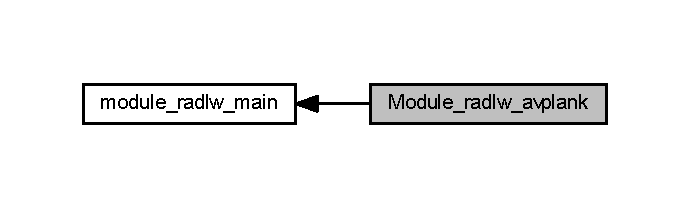
\includegraphics[width=331pt]{group__module__radlw__avplank}
\end{center}
\end{figure}

\hypertarget{group__module__radlw__cldprlw}{}\section{Module\+\_\+radlw\+\_\+cldprlw}
\label{group__module__radlw__cldprlw}\index{Module\+\_\+radlw\+\_\+cldprlw@{Module\+\_\+radlw\+\_\+cldprlw}}


This module contains cloud property coefficients.  


Collaboration diagram for Module\+\_\+radlw\+\_\+cldprlw\+:\nopagebreak
\begin{figure}[H]
\begin{center}
\leavevmode
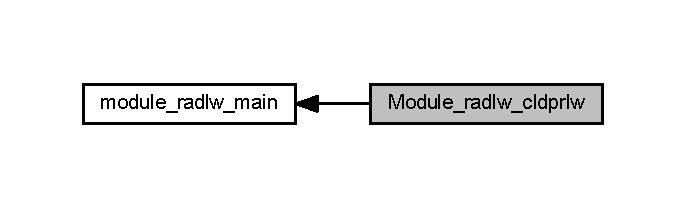
\includegraphics[width=329pt]{group__module__radlw__cldprlw}
\end{center}
\end{figure}

\hypertarget{group__module__radlw__kgb01}{}\section{Module\+\_\+radlw\+\_\+kgb01}
\label{group__module__radlw__kgb01}\index{Module\+\_\+radlw\+\_\+kgb01@{Module\+\_\+radlw\+\_\+kgb01}}


This module sets up absorption coefficients for band 01\+: 10-\/250 cm-\/1 (low -\/ h2o; high -\/ h2o)  


Collaboration diagram for Module\+\_\+radlw\+\_\+kgb01\+:\nopagebreak
\begin{figure}[H]
\begin{center}
\leavevmode
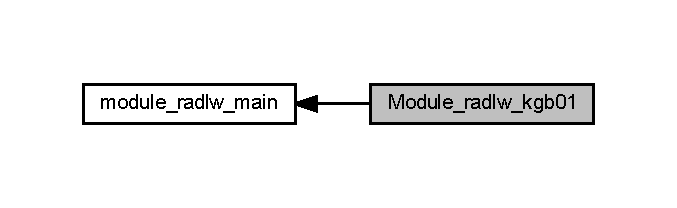
\includegraphics[width=325pt]{group__module__radlw__kgb01}
\end{center}
\end{figure}

\hypertarget{group__module__radlw__kgb02}{}\section{Module\+\_\+radlw\+\_\+kgb02}
\label{group__module__radlw__kgb02}\index{Module\+\_\+radlw\+\_\+kgb02@{Module\+\_\+radlw\+\_\+kgb02}}


This module sets up absorption coefficients for band 02\+: 250-\/500 cm-\/1 (low -\/ h2o; high -\/ h2o)  


Collaboration diagram for Module\+\_\+radlw\+\_\+kgb02\+:\nopagebreak
\begin{figure}[H]
\begin{center}
\leavevmode
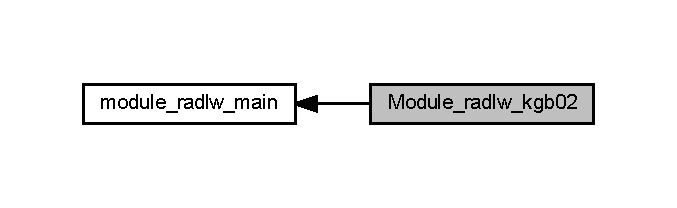
\includegraphics[width=325pt]{group__module__radlw__kgb02}
\end{center}
\end{figure}

\hypertarget{group__module__radlw__kgb03}{}\section{Module\+\_\+radlw\+\_\+kgb03}
\label{group__module__radlw__kgb03}\index{Module\+\_\+radlw\+\_\+kgb03@{Module\+\_\+radlw\+\_\+kgb03}}


This module sets up absorption coefficients for band 03\+: 500-\/630 cm-\/1 (low -\/ h2o, co2; high -\/ h2o, co2)  


Collaboration diagram for Module\+\_\+radlw\+\_\+kgb03\+:\nopagebreak
\begin{figure}[H]
\begin{center}
\leavevmode
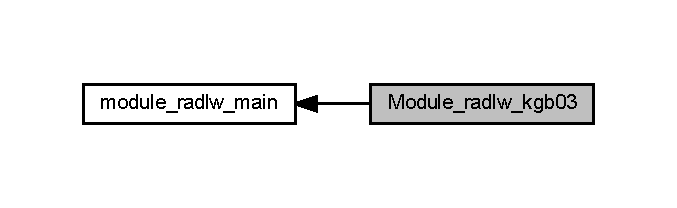
\includegraphics[width=325pt]{group__module__radlw__kgb03}
\end{center}
\end{figure}

\hypertarget{group__module__radlw__kgb04}{}\section{Module\+\_\+radlw\+\_\+kgb04}
\label{group__module__radlw__kgb04}\index{Module\+\_\+radlw\+\_\+kgb04@{Module\+\_\+radlw\+\_\+kgb04}}


This module sets up absorption coefficients for band 04\+: 630-\/700 cm-\/1 (low -\/ h2o, co2; high -\/ co2, o3)  


Collaboration diagram for Module\+\_\+radlw\+\_\+kgb04\+:\nopagebreak
\begin{figure}[H]
\begin{center}
\leavevmode
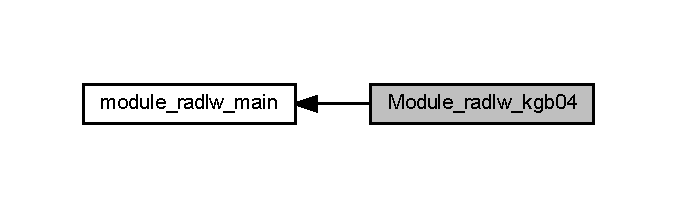
\includegraphics[width=325pt]{group__module__radlw__kgb04}
\end{center}
\end{figure}

\hypertarget{group__module__radlw__kgb05}{}\section{Module\+\_\+radlw\+\_\+kgb05}
\label{group__module__radlw__kgb05}\index{Module\+\_\+radlw\+\_\+kgb05@{Module\+\_\+radlw\+\_\+kgb05}}


This module sets up absorption coefficients for band 05\+: 700-\/820 cm-\/1 (low -\/ h2o, co2; high -\/ co2, o3)  


Collaboration diagram for Module\+\_\+radlw\+\_\+kgb05\+:\nopagebreak
\begin{figure}[H]
\begin{center}
\leavevmode
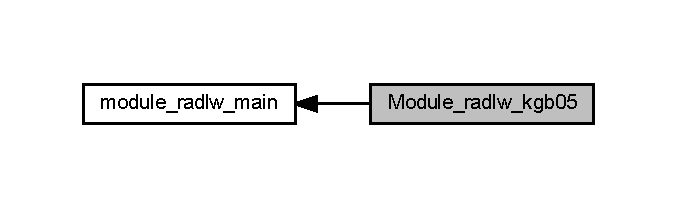
\includegraphics[width=325pt]{group__module__radlw__kgb05}
\end{center}
\end{figure}

\hypertarget{group__module__radlw__kgb06}{}\section{Module\+\_\+radlw\+\_\+kgb06}
\label{group__module__radlw__kgb06}\index{Module\+\_\+radlw\+\_\+kgb06@{Module\+\_\+radlw\+\_\+kgb06}}


This module sets up absorption coefficients for band 06\+: 820-\/980 cm-\/1 (low -\/ h2o; high -\/ /)  


Collaboration diagram for Module\+\_\+radlw\+\_\+kgb06\+:\nopagebreak
\begin{figure}[H]
\begin{center}
\leavevmode
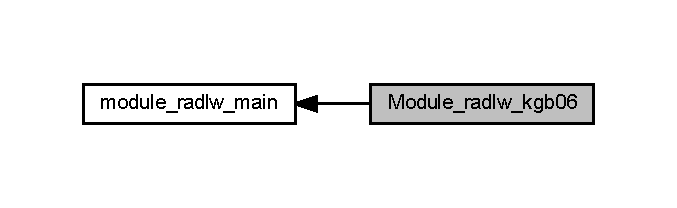
\includegraphics[width=325pt]{group__module__radlw__kgb06}
\end{center}
\end{figure}

\hypertarget{group__module__radlw__kgb07}{}\section{Module\+\_\+radlw\+\_\+kgb07}
\label{group__module__radlw__kgb07}\index{Module\+\_\+radlw\+\_\+kgb07@{Module\+\_\+radlw\+\_\+kgb07}}


This module sets up absorption coefficients for band 07\+: 980-\/1080 cm-\/1 (low -\/ h2o, o3; high -\/ o3)  


Collaboration diagram for Module\+\_\+radlw\+\_\+kgb07\+:\nopagebreak
\begin{figure}[H]
\begin{center}
\leavevmode
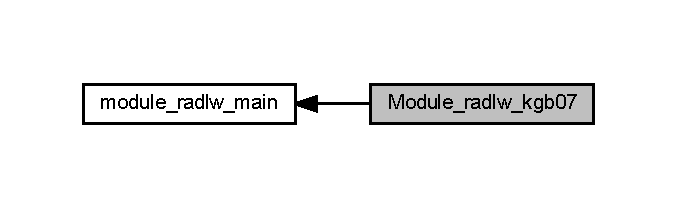
\includegraphics[width=325pt]{group__module__radlw__kgb07}
\end{center}
\end{figure}

\hypertarget{group__module__radlw__kgb08}{}\section{Module\+\_\+radlw\+\_\+kgb08}
\label{group__module__radlw__kgb08}\index{Module\+\_\+radlw\+\_\+kgb08@{Module\+\_\+radlw\+\_\+kgb08}}


This module sets up absorption coefficients for band 08\+: 1080-\/1180 cm-\/1 (low -\/ h2o; high -\/ o3)  


Collaboration diagram for Module\+\_\+radlw\+\_\+kgb08\+:\nopagebreak
\begin{figure}[H]
\begin{center}
\leavevmode
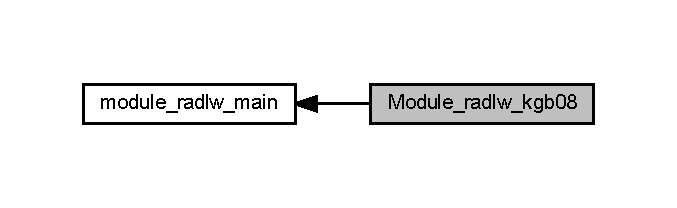
\includegraphics[width=325pt]{group__module__radlw__kgb08}
\end{center}
\end{figure}

\hypertarget{group__module__radlw__kgb09}{}\section{Module\+\_\+radlw\+\_\+kgb09}
\label{group__module__radlw__kgb09}\index{Module\+\_\+radlw\+\_\+kgb09@{Module\+\_\+radlw\+\_\+kgb09}}


This module sets up absorption coefficients for band 09\+: 1180-\/1390 cm-\/1 (low -\/ h2o, ch4; high -\/ ch4)  


Collaboration diagram for Module\+\_\+radlw\+\_\+kgb09\+:\nopagebreak
\begin{figure}[H]
\begin{center}
\leavevmode
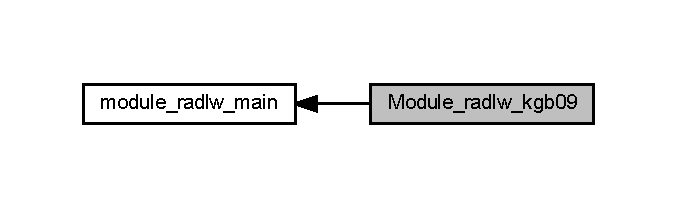
\includegraphics[width=325pt]{group__module__radlw__kgb09}
\end{center}
\end{figure}

\hypertarget{group__module__radlw__kgb10}{}\section{Module\+\_\+radlw\+\_\+kgb10}
\label{group__module__radlw__kgb10}\index{Module\+\_\+radlw\+\_\+kgb10@{Module\+\_\+radlw\+\_\+kgb10}}


This module sets up absorption coefficients for band 10\+: 1390-\/1480 cm-\/1 (low -\/ h2o; high -\/ h2o)  


Collaboration diagram for Module\+\_\+radlw\+\_\+kgb10\+:\nopagebreak
\begin{figure}[H]
\begin{center}
\leavevmode
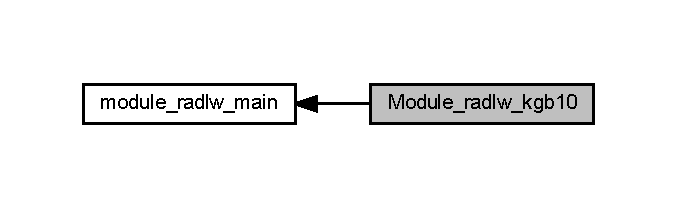
\includegraphics[width=325pt]{group__module__radlw__kgb10}
\end{center}
\end{figure}

\hypertarget{group__module__radlw__kgb11}{}\section{Module\+\_\+radlw\+\_\+kgb11}
\label{group__module__radlw__kgb11}\index{Module\+\_\+radlw\+\_\+kgb11@{Module\+\_\+radlw\+\_\+kgb11}}


This module sets up absorption coefficients for band 11\+: 1480-\/1800 cm-\/1 (low -\/ h2o; high -\/ h2o)  


Collaboration diagram for Module\+\_\+radlw\+\_\+kgb11\+:\nopagebreak
\begin{figure}[H]
\begin{center}
\leavevmode
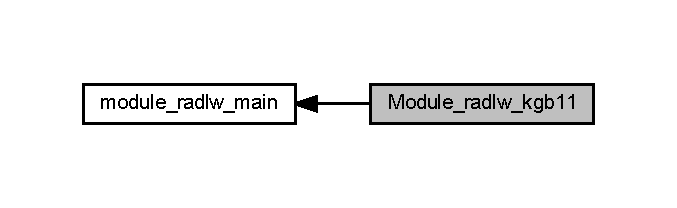
\includegraphics[width=325pt]{group__module__radlw__kgb11}
\end{center}
\end{figure}

\hypertarget{group__module__radlw__kgb12}{}\section{Module\+\_\+radlw\+\_\+kgb12}
\label{group__module__radlw__kgb12}\index{Module\+\_\+radlw\+\_\+kgb12@{Module\+\_\+radlw\+\_\+kgb12}}


This module sets up absorption coefficients for band 12\+: 1800-\/2080 cm-\/1 (low -\/ h2o, co2; high -\/ /)  


Collaboration diagram for Module\+\_\+radlw\+\_\+kgb12\+:\nopagebreak
\begin{figure}[H]
\begin{center}
\leavevmode
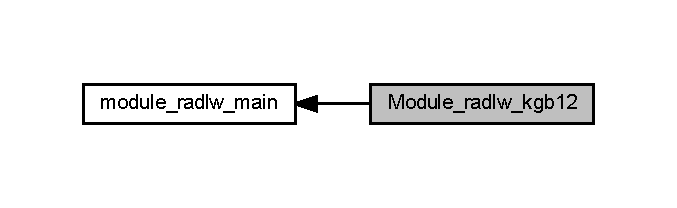
\includegraphics[width=325pt]{group__module__radlw__kgb12}
\end{center}
\end{figure}

\hypertarget{group__module__radlw__kgb13}{}\section{Module\+\_\+radlw\+\_\+kgb13}
\label{group__module__radlw__kgb13}\index{Module\+\_\+radlw\+\_\+kgb13@{Module\+\_\+radlw\+\_\+kgb13}}


This module sets up absorption coefficients for band 13\+: 2080-\/2250 cm-\/1 (low -\/ h2o, n2o; high -\/ /)  


Collaboration diagram for Module\+\_\+radlw\+\_\+kgb13\+:\nopagebreak
\begin{figure}[H]
\begin{center}
\leavevmode
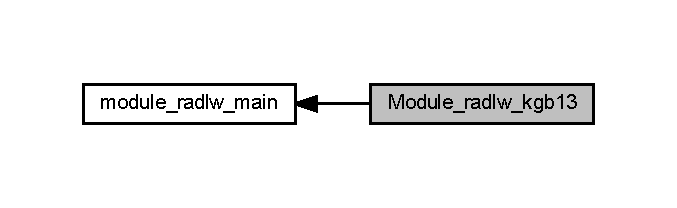
\includegraphics[width=325pt]{group__module__radlw__kgb13}
\end{center}
\end{figure}

\hypertarget{group__module__radlw__kgb14}{}\section{Module\+\_\+radlw\+\_\+kgb14}
\label{group__module__radlw__kgb14}\index{Module\+\_\+radlw\+\_\+kgb14@{Module\+\_\+radlw\+\_\+kgb14}}


This module sets up absorption coefficients for band 14\+: 2250-\/2380 cm-\/1 (low -\/ co2; high -\/ co2)  


Collaboration diagram for Module\+\_\+radlw\+\_\+kgb14\+:\nopagebreak
\begin{figure}[H]
\begin{center}
\leavevmode
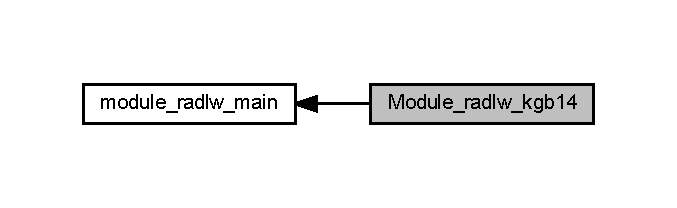
\includegraphics[width=325pt]{group__module__radlw__kgb14}
\end{center}
\end{figure}

\hypertarget{group__module__radlw__kgb15}{}\section{Module\+\_\+radlw\+\_\+kgb15}
\label{group__module__radlw__kgb15}\index{Module\+\_\+radlw\+\_\+kgb15@{Module\+\_\+radlw\+\_\+kgb15}}


This module sets up absorption coefficients for band 15\+: 2380-\/2600 cm-\/1 (low -\/ n2o, co2; high -\/ /)  


Collaboration diagram for Module\+\_\+radlw\+\_\+kgb15\+:\nopagebreak
\begin{figure}[H]
\begin{center}
\leavevmode
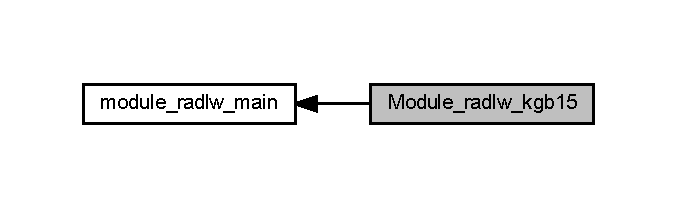
\includegraphics[width=325pt]{group__module__radlw__kgb15}
\end{center}
\end{figure}

\hypertarget{group__module__radlw__kgb16}{}\section{Module\+\_\+radlw\+\_\+kgb16}
\label{group__module__radlw__kgb16}\index{Module\+\_\+radlw\+\_\+kgb16@{Module\+\_\+radlw\+\_\+kgb16}}


This module sets up absorption coefficients for band 16\+: 2600-\/3000 cm-\/1 (low -\/ h2o, ch4; high -\/ /)  


Collaboration diagram for Module\+\_\+radlw\+\_\+kgb16\+:\nopagebreak
\begin{figure}[H]
\begin{center}
\leavevmode
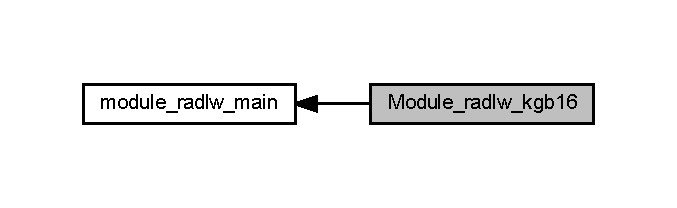
\includegraphics[width=325pt]{group__module__radlw__kgb16}
\end{center}
\end{figure}

\hypertarget{group__module__radlw__parameters}{}\section{Module\+\_\+radlw\+\_\+parameters}
\label{group__module__radlw__parameters}\index{Module\+\_\+radlw\+\_\+parameters@{Module\+\_\+radlw\+\_\+parameters}}


This module contains LW band parameters set up.  


Collaboration diagram for Module\+\_\+radlw\+\_\+parameters\+:\nopagebreak
\begin{figure}[H]
\begin{center}
\leavevmode
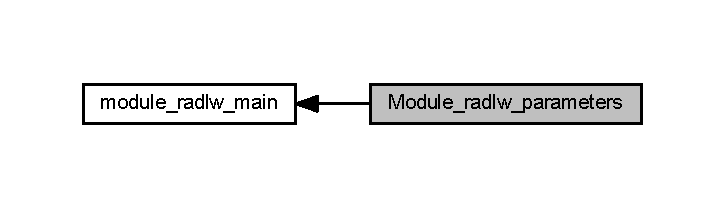
\includegraphics[width=348pt]{group__module__radlw__parameters}
\end{center}
\end{figure}

\hypertarget{group__module__radlw__ref}{}\section{Module\+\_\+radlw\+\_\+ref}
\label{group__module__radlw__ref}\index{Module\+\_\+radlw\+\_\+ref@{Module\+\_\+radlw\+\_\+ref}}


This module contains reference temperature and pressure.  


Collaboration diagram for Module\+\_\+radlw\+\_\+ref\+:\nopagebreak
\begin{figure}[H]
\begin{center}
\leavevmode
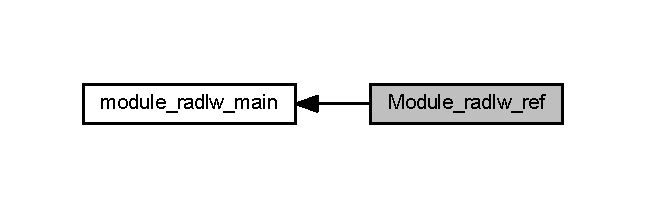
\includegraphics[width=310pt]{group__module__radlw__ref}
\end{center}
\end{figure}

\hypertarget{group__module__radsw__cldprtb}{}\section{Module\+\_\+radsw\+\_\+cldprtb}
\label{group__module__radsw__cldprtb}\index{Module\+\_\+radsw\+\_\+cldprtb@{Module\+\_\+radsw\+\_\+cldprtb}}


This module contains coefficients of cloud optical properties for each of the spectral bands. It is modified from A\+E\+R/\+E\+C\+M\+WF R\+R\+TM SW radiation package subroutine \char`\"{}susrtop\char`\"{}.  


Collaboration diagram for Module\+\_\+radsw\+\_\+cldprtb\+:\nopagebreak
\begin{figure}[H]
\begin{center}
\leavevmode
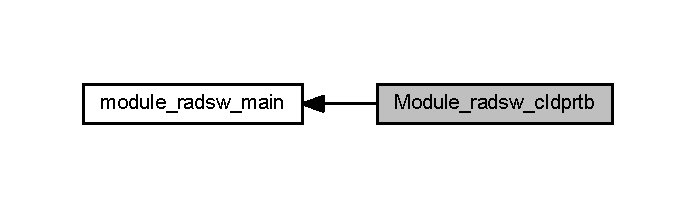
\includegraphics[width=334pt]{group__module__radsw__cldprtb}
\end{center}
\end{figure}

\hypertarget{group__module__radsw__kgb16}{}\section{Module\+\_\+radsw\+\_\+kgb16}
\label{group__module__radsw__kgb16}\index{Module\+\_\+radsw\+\_\+kgb16@{Module\+\_\+radsw\+\_\+kgb16}}


This module sets up absorption coefficients for band 16\+: 2600-\/3250 cm-\/1 (low -\/ h2o, ch4; high -\/ ch4)  


Collaboration diagram for Module\+\_\+radsw\+\_\+kgb16\+:\nopagebreak
\begin{figure}[H]
\begin{center}
\leavevmode
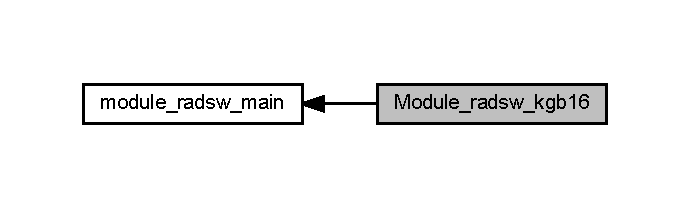
\includegraphics[width=331pt]{group__module__radsw__kgb16}
\end{center}
\end{figure}

\hypertarget{group__module__radsw__kgb17}{}\section{Module\+\_\+radsw\+\_\+kgb17}
\label{group__module__radsw__kgb17}\index{Module\+\_\+radsw\+\_\+kgb17@{Module\+\_\+radsw\+\_\+kgb17}}


This module sets up absorption coeffients for band 17\+: 3250-\/4000 cm-\/1 (low -\/ h2o,co2; high -\/ h2o,co2)  


Collaboration diagram for Module\+\_\+radsw\+\_\+kgb17\+:\nopagebreak
\begin{figure}[H]
\begin{center}
\leavevmode
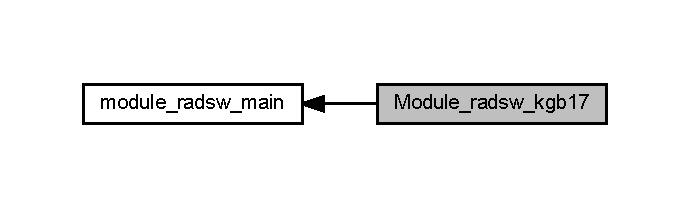
\includegraphics[width=331pt]{group__module__radsw__kgb17}
\end{center}
\end{figure}

\hypertarget{group__module__radsw__kgb18}{}\section{Module\+\_\+radsw\+\_\+kgb18}
\label{group__module__radsw__kgb18}\index{Module\+\_\+radsw\+\_\+kgb18@{Module\+\_\+radsw\+\_\+kgb18}}


This module sets up absorption coeffients for band 18\+: 4000-\/4650 cm-\/1 (low -\/ h2o,ch4; high -\/ ch4)  


Collaboration diagram for Module\+\_\+radsw\+\_\+kgb18\+:\nopagebreak
\begin{figure}[H]
\begin{center}
\leavevmode
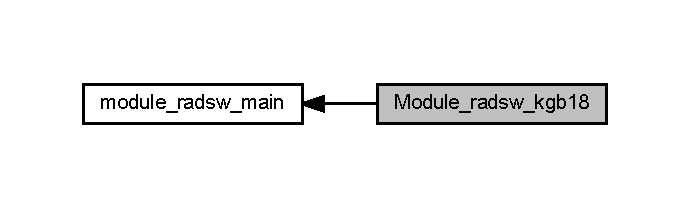
\includegraphics[width=331pt]{group__module__radsw__kgb18}
\end{center}
\end{figure}

\hypertarget{group__module__radsw__kgb19}{}\section{Module\+\_\+radsw\+\_\+kgb19}
\label{group__module__radsw__kgb19}\index{Module\+\_\+radsw\+\_\+kgb19@{Module\+\_\+radsw\+\_\+kgb19}}


This module sets up absorption coeffients for band 19\+: 4650-\/5150 cm-\/1 (low -\/ h2o,co2; high -\/ co2)  


Collaboration diagram for Module\+\_\+radsw\+\_\+kgb19\+:\nopagebreak
\begin{figure}[H]
\begin{center}
\leavevmode
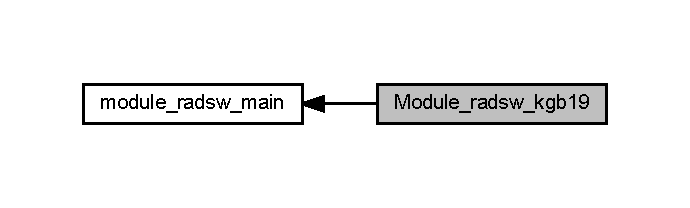
\includegraphics[width=331pt]{group__module__radsw__kgb19}
\end{center}
\end{figure}

\hypertarget{group__module__radsw__kgb20}{}\section{Module\+\_\+radsw\+\_\+kgb20}
\label{group__module__radsw__kgb20}\index{Module\+\_\+radsw\+\_\+kgb20@{Module\+\_\+radsw\+\_\+kgb20}}


This module sets up absorption coeffients for band 20\+: 5150-\/6150 cm-\/1 (low -\/ h2o; high -\/ h2o)  


Collaboration diagram for Module\+\_\+radsw\+\_\+kgb20\+:\nopagebreak
\begin{figure}[H]
\begin{center}
\leavevmode
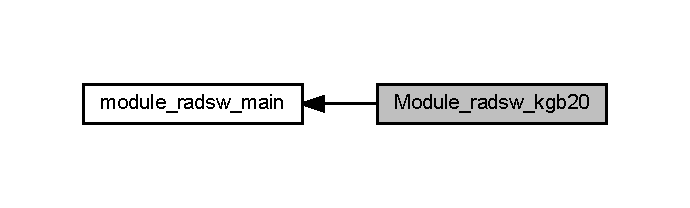
\includegraphics[width=331pt]{group__module__radsw__kgb20}
\end{center}
\end{figure}

\hypertarget{group__module__radsw__kgb21}{}\section{Module\+\_\+radsw\+\_\+kgb21}
\label{group__module__radsw__kgb21}\index{Module\+\_\+radsw\+\_\+kgb21@{Module\+\_\+radsw\+\_\+kgb21}}


This module sets up absorption coeffients for band 21\+: 6150-\/7700 cm-\/1 (low -\/ h2o,co2; high -\/ h2o,co2)  


Collaboration diagram for Module\+\_\+radsw\+\_\+kgb21\+:\nopagebreak
\begin{figure}[H]
\begin{center}
\leavevmode
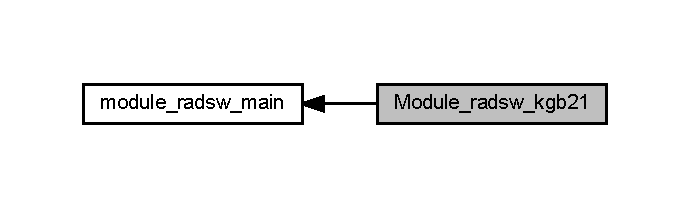
\includegraphics[width=331pt]{group__module__radsw__kgb21}
\end{center}
\end{figure}

\hypertarget{group__module__radsw__kgb22}{}\section{Module\+\_\+radsw\+\_\+kgb22}
\label{group__module__radsw__kgb22}\index{Module\+\_\+radsw\+\_\+kgb22@{Module\+\_\+radsw\+\_\+kgb22}}


This module sets up absorption coeffients for band 22\+: 7700-\/8050 cm-\/1 (low -\/ h2o, o2; high -\/ o2)  


Collaboration diagram for Module\+\_\+radsw\+\_\+kgb22\+:\nopagebreak
\begin{figure}[H]
\begin{center}
\leavevmode
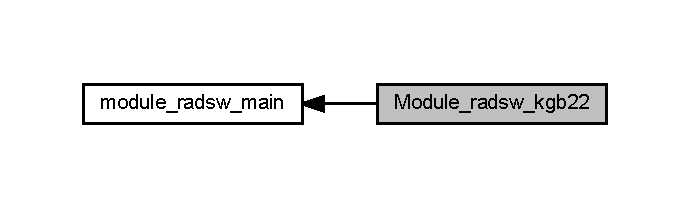
\includegraphics[width=331pt]{group__module__radsw__kgb22}
\end{center}
\end{figure}

\hypertarget{group__module__radsw__kgb23}{}\section{Module\+\_\+radsw\+\_\+kgb23}
\label{group__module__radsw__kgb23}\index{Module\+\_\+radsw\+\_\+kgb23@{Module\+\_\+radsw\+\_\+kgb23}}


This module sets up absorption coeffients for band 23\+: 8050-\/12850 cm-\/1 (low -\/ h2o; high -\/ nothing)  


Collaboration diagram for Module\+\_\+radsw\+\_\+kgb23\+:\nopagebreak
\begin{figure}[H]
\begin{center}
\leavevmode
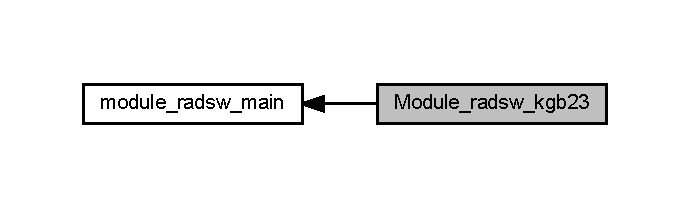
\includegraphics[width=331pt]{group__module__radsw__kgb23}
\end{center}
\end{figure}

\hypertarget{group__module__radsw__kgb24}{}\section{Module\+\_\+radsw\+\_\+kgb24}
\label{group__module__radsw__kgb24}\index{Module\+\_\+radsw\+\_\+kgb24@{Module\+\_\+radsw\+\_\+kgb24}}


This module sets up absorption coeffients for band 24\+: 12850-\/16000 cm-\/1 (low -\/ h2o, o2; high -\/ o2)  


Collaboration diagram for Module\+\_\+radsw\+\_\+kgb24\+:\nopagebreak
\begin{figure}[H]
\begin{center}
\leavevmode
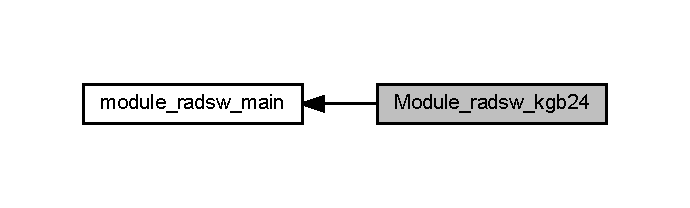
\includegraphics[width=331pt]{group__module__radsw__kgb24}
\end{center}
\end{figure}

\hypertarget{group__module__radsw__kgb25}{}\section{Module\+\_\+radsw\+\_\+kgb25}
\label{group__module__radsw__kgb25}\index{Module\+\_\+radsw\+\_\+kgb25@{Module\+\_\+radsw\+\_\+kgb25}}


This module sets up absorption coeffients for band 25\+: 16000-\/22650 cm-\/1 (low -\/ h2o; high -\/ nothing)  


Collaboration diagram for Module\+\_\+radsw\+\_\+kgb25\+:\nopagebreak
\begin{figure}[H]
\begin{center}
\leavevmode
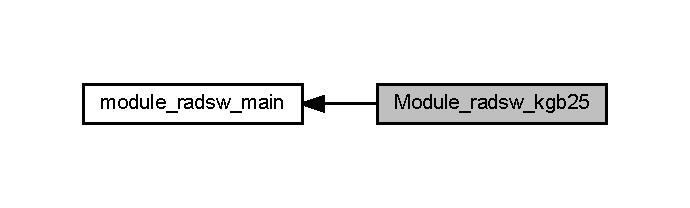
\includegraphics[width=331pt]{group__module__radsw__kgb25}
\end{center}
\end{figure}

\hypertarget{group__module__radsw__kgb26}{}\section{Module\+\_\+radsw\+\_\+kgb26}
\label{group__module__radsw__kgb26}\index{Module\+\_\+radsw\+\_\+kgb26@{Module\+\_\+radsw\+\_\+kgb26}}


This module sets up absorption coeffients for band 26\+: 22650-\/29000 cm-\/1 (low -\/ nothing; high -\/ nothing)  


Collaboration diagram for Module\+\_\+radsw\+\_\+kgb26\+:\nopagebreak
\begin{figure}[H]
\begin{center}
\leavevmode
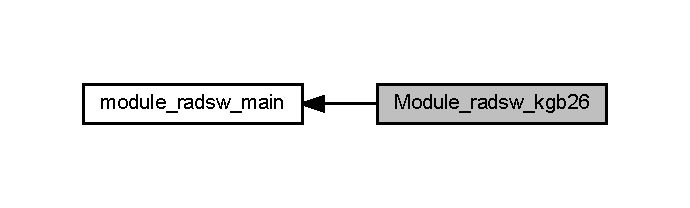
\includegraphics[width=331pt]{group__module__radsw__kgb26}
\end{center}
\end{figure}

\hypertarget{group__module__radsw__kgb27}{}\section{Module\+\_\+radsw\+\_\+kgb27}
\label{group__module__radsw__kgb27}\index{Module\+\_\+radsw\+\_\+kgb27@{Module\+\_\+radsw\+\_\+kgb27}}


This module sets up absorption coeffients for band 27\+: 29000-\/38000 cm-\/1 (low -\/ o3; high -\/ o3)  


Collaboration diagram for Module\+\_\+radsw\+\_\+kgb27\+:\nopagebreak
\begin{figure}[H]
\begin{center}
\leavevmode
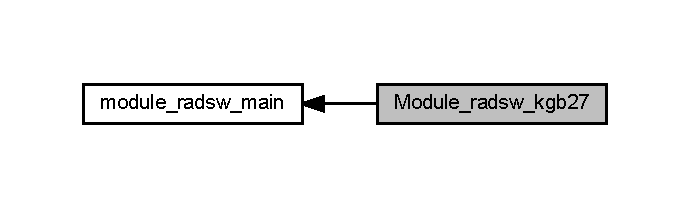
\includegraphics[width=331pt]{group__module__radsw__kgb27}
\end{center}
\end{figure}

\hypertarget{group__module__radsw__kgb28}{}\section{Module\+\_\+radsw\+\_\+kgb28}
\label{group__module__radsw__kgb28}\index{Module\+\_\+radsw\+\_\+kgb28@{Module\+\_\+radsw\+\_\+kgb28}}


This module sets up absorption coeffients for band 28\+: 38000-\/50000 cm-\/1 (low -\/ o3,o2; high -\/ o3,o2)  


Collaboration diagram for Module\+\_\+radsw\+\_\+kgb28\+:\nopagebreak
\begin{figure}[H]
\begin{center}
\leavevmode
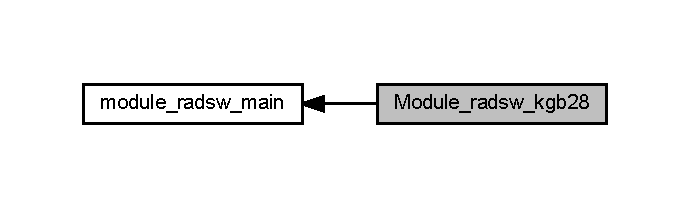
\includegraphics[width=331pt]{group__module__radsw__kgb28}
\end{center}
\end{figure}

\hypertarget{group__module__radsw__kgb29}{}\section{Module\+\_\+radsw\+\_\+kgb29}
\label{group__module__radsw__kgb29}\index{Module\+\_\+radsw\+\_\+kgb29@{Module\+\_\+radsw\+\_\+kgb29}}


This module sets up absorption coeffients for band 29\+: 820-\/2600 cm-\/1 (low -\/ h2o; high -\/ co2)  


Collaboration diagram for Module\+\_\+radsw\+\_\+kgb29\+:\nopagebreak
\begin{figure}[H]
\begin{center}
\leavevmode
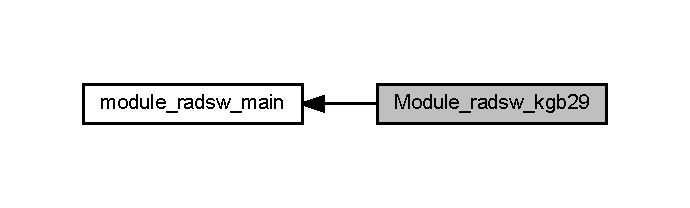
\includegraphics[width=331pt]{group__module__radsw__kgb29}
\end{center}
\end{figure}

\hypertarget{group__module__radsw__parameters}{}\section{Module\+\_\+radsw\+\_\+parameters}
\label{group__module__radsw__parameters}\index{Module\+\_\+radsw\+\_\+parameters@{Module\+\_\+radsw\+\_\+parameters}}


This module contains SW band parameters set up.  


Collaboration diagram for Module\+\_\+radsw\+\_\+parameters\+:\nopagebreak
\begin{figure}[H]
\begin{center}
\leavevmode
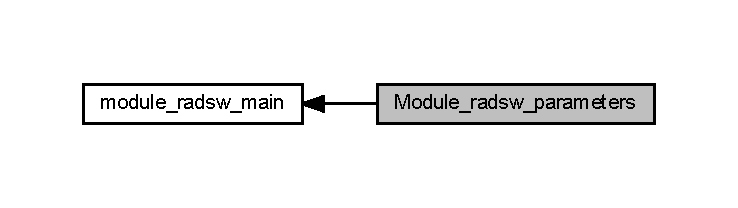
\includegraphics[width=350pt]{group__module__radsw__parameters}
\end{center}
\end{figure}

\hypertarget{group__module__radsw__ref}{}\section{Module\+\_\+radsw\+\_\+ref}
\label{group__module__radsw__ref}\index{Module\+\_\+radsw\+\_\+ref@{Module\+\_\+radsw\+\_\+ref}}


This module contains reference temperature and pressure.  


Collaboration diagram for Module\+\_\+radsw\+\_\+ref\+:\nopagebreak
\begin{figure}[H]
\begin{center}
\leavevmode
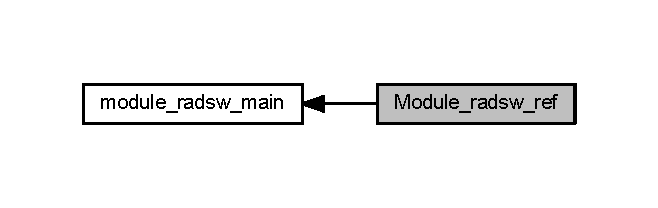
\includegraphics[width=316pt]{group__module__radsw__ref}
\end{center}
\end{figure}

\hypertarget{group__module__radsw__sflux}{}\section{Module\+\_\+radsw\+\_\+sflux}
\label{group__module__radsw__sflux}\index{Module\+\_\+radsw\+\_\+sflux@{Module\+\_\+radsw\+\_\+sflux}}


This module contains spectral distribution of solar radiation flux used to obtain the incoming solar flux at toa.  


Collaboration diagram for Module\+\_\+radsw\+\_\+sflux\+:\nopagebreak
\begin{figure}[H]
\begin{center}
\leavevmode
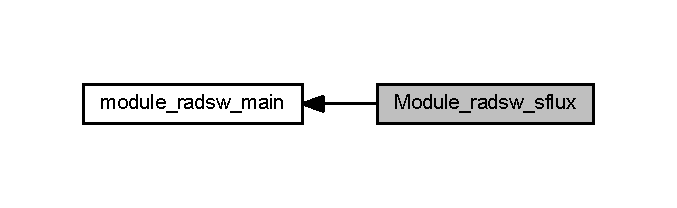
\includegraphics[width=325pt]{group__module__radsw__sflux}
\end{center}
\end{figure}

\hypertarget{group__rad}{}\section{R\+R\+T\+MG Radiation Scheme}
\label{group__rad}\index{R\+R\+T\+M\+G Radiation Scheme@{R\+R\+T\+M\+G Radiation Scheme}}


one line description  


Collaboration diagram for R\+R\+T\+MG Radiation Scheme\+:\nopagebreak
\begin{figure}[H]
\begin{center}
\leavevmode
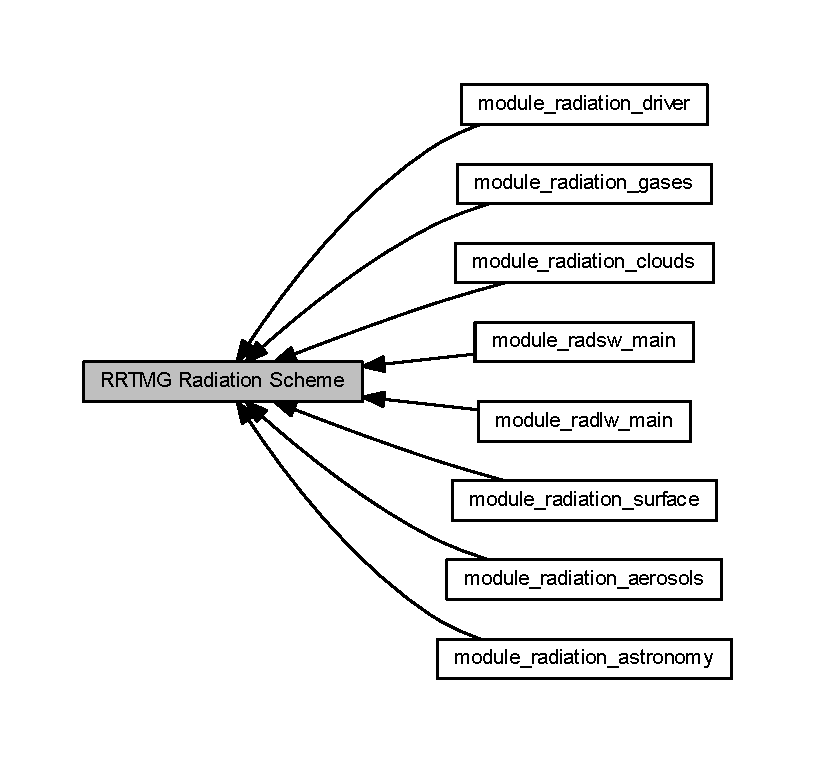
\includegraphics[width=350pt]{group__rad}
\end{center}
\end{figure}
\subsection*{Modules}
\begin{DoxyCompactItemize}
\item 
\hyperlink{group__module__radiation__aerosols}{module\+\_\+radiation\+\_\+aerosols}
\begin{DoxyCompactList}\small\item\em This module contains climatological atmospheric aerosol schemes for radiation computations. \end{DoxyCompactList}\item 
\hyperlink{group__module__radiation__astronomy}{module\+\_\+radiation\+\_\+astronomy}
\begin{DoxyCompactList}\small\item\em This module sets up astronomy quantities for solar radiation calculations. \end{DoxyCompactList}\item 
\hyperlink{group__module__radiation__clouds}{module\+\_\+radiation\+\_\+clouds}
\begin{DoxyCompactList}\small\item\em This module computes cloud related quantities for radiation computations. \end{DoxyCompactList}\item 
\hyperlink{group__module__radiation__driver}{module\+\_\+radiation\+\_\+driver}
\begin{DoxyCompactList}\small\item\em \hyperlink{namespacemodule__radiation__driver}{module\+\_\+radiation\+\_\+driver} prepares atmospheric profile, invokes main radiation calculations, and computes radiative fluxes and heating rates for some arbitrary number of vertical colums.\+There are three externally accessible subroutines\+: radinit, radupdate, and grrad. \end{DoxyCompactList}\item 
\hyperlink{group__module__radiation__gases}{module\+\_\+radiation\+\_\+gases}
\begin{DoxyCompactList}\small\item\em This module sets up ozone climatological profiles and other constant gas profiles, such as co2, ch4, n2o, o2, and those of cfc gases. All data are entered as mixing ratio by volume, except ozone which is mass mixing ratio (g/g). \end{DoxyCompactList}\item 
\hyperlink{group__module__radiation__surface}{module\+\_\+radiation\+\_\+surface}
\begin{DoxyCompactList}\small\item\em This module sets up surface albedo for sw radiation and surface emissivity for lw radiation. \end{DoxyCompactList}\item 
\hyperlink{group__module__radlw__main}{module\+\_\+radlw\+\_\+main}
\begin{DoxyCompactList}\small\item\em This module includes ncep\textquotesingle{}s modifications of the rrtm-\/lw radiation code from aer inc. \end{DoxyCompactList}\item 
\hyperlink{group__module__radsw__main}{module\+\_\+radsw\+\_\+main}
\begin{DoxyCompactList}\small\item\em This module includes ncep\textquotesingle{}s modifications of the rrtm-\/sw radiation code from aer inc. \end{DoxyCompactList}\end{DoxyCompactItemize}


\subsection{Detailed Description}
Radiative process is one of the most complex and computational intensive part of all model physics. As an essential part of model physics, it directly and indirectly connects all physics processes with model dynamics, and regulates the overall earth-\/atmosphere energy exchanges and transformations. The radiation package in N\+E\+MS physics has standardized component modules. The schematic radiation module structure is shown in table 1.

Radiation parameterizations are intended to provide a fast and accurate method of determined the total radiative flux at any given location. These calculations provide both the total radiative flux at the ground surface, which is needed for the surface energy budget, and the vertical radiative flux divergence, which is used to calculate the radiative heating and cooling rates of a given atmospheric volume. The magnitude of the terms in the surface energy budget can set the stage for moist deep convection and are crucial to the formation of low-\/level clouds. In addition, the vertical radiative flux divergence can produce substantial cooling, particularly at the tops of clouds, which can have strong dynamic effect on cloud evolution.\hypertarget{group__rad_diagram}{}\subsection{Calling Hierarchy Diagram}\label{group__rad_diagram}
 \hypertarget{group__rad_intraphysics}{}\subsection{Intraphysics Communication}\label{group__rad_intraphysics}
This space is reserved for a description of how this scheme uses information from other scheme types and/or how information calculated in this scheme is used in other scheme types. \hypertarget{group__rad_mainpage-components}{}\subsection{Radiation Scheme Modules}\label{group__rad_mainpage-components}
The following links take you to more information about each module.
\begin{DoxyItemize}
\item Driver Module\+: \hyperlink{group__module__radiation__driver}{module\+\_\+radiation\+\_\+driver}
\item Shortwave(\+S\+W) Module\+: \hyperlink{group__module__radsw__main}{module\+\_\+radsw\+\_\+main}
\item Longwave(\+L\+W) Module\+: \hyperlink{group__module__radlw__main}{module\+\_\+radlw\+\_\+main}
\item Astronomy Module\+: \hyperlink{group__module__radiation__astronomy}{module\+\_\+radiation\+\_\+astronomy}
\item Aerosol Module\+: \hyperlink{group__module__radiation__aerosols}{module\+\_\+radiation\+\_\+aerosols}
\item Cloud Module\+: \hyperlink{group__module__radiation__clouds}{module\+\_\+radiation\+\_\+clouds}
\item Surface Module\+: \hyperlink{group__module__radiation__surface}{module\+\_\+radiation\+\_\+surface}
\item Gases Module\+: \hyperlink{group__module__radiation__gases}{module\+\_\+radiation\+\_\+gases} 
\end{DoxyItemize}
\hypertarget{group__module__radiation__aerosols}{}\section{module\+\_\+radiation\+\_\+aerosols}
\label{group__module__radiation__aerosols}\index{module\+\_\+radiation\+\_\+aerosols@{module\+\_\+radiation\+\_\+aerosols}}


This module contains climatological atmospheric aerosol schemes for radiation computations.  


Collaboration diagram for module\+\_\+radiation\+\_\+aerosols\+:\nopagebreak
\begin{figure}[H]
\begin{center}
\leavevmode
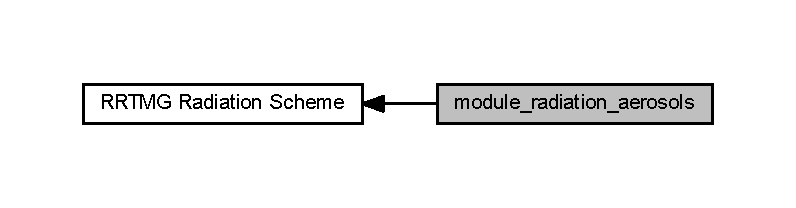
\includegraphics[width=350pt]{group__module__radiation__aerosols}
\end{center}
\end{figure}
\subsection*{Modules}
\begin{DoxyCompactItemize}
\item 
module \hyperlink{namespacemodule__radiation__aerosols}{module\+\_\+radiation\+\_\+aerosols}
\end{DoxyCompactItemize}
\subsection*{Data Types}
\begin{DoxyCompactItemize}
\item 
type \hyperlink{structmodule__radiation__aerosols_1_1gocart__index__type}{module\+\_\+radiation\+\_\+aerosols\+::gocart\+\_\+index\+\_\+type}
\item 
type \hyperlink{structmodule__radiation__aerosols_1_1tracer__index__type}{module\+\_\+radiation\+\_\+aerosols\+::tracer\+\_\+index\+\_\+type}
\end{DoxyCompactItemize}
\subsection*{Functions/\+Subroutines}
\begin{DoxyCompactItemize}
\item 
subroutine, public \hyperlink{group__module__radiation__aerosols_gabe52f1b6f62b158154e70a7b5058ad20}{module\+\_\+radiation\+\_\+aerosols\+::aer\+\_\+init}
\begin{DoxyCompactList}\small\item\em The initialization program to set up necessary parameters and working arrays. \end{DoxyCompactList}\item 
subroutine \hyperlink{group__module__radiation__aerosols_ga3135fdf318002f9d56dd2d93225f4aac}{wrt\+\_\+aerlog}
\begin{DoxyCompactList}\small\item\em This subroutine writes aerosol parameter configuration to run log file. \end{DoxyCompactList}\item 
subroutine \hyperlink{group__module__radiation__aerosols_gaa7fe6dc2964bc474a132b93aaab82cb0}{set\+\_\+spectrum}
\begin{DoxyCompactList}\small\item\em This subroutine defines the one wavenumber solar fluxes based on toa solar spectral distribution, and define the one wavenumber IR fluxes based on black-\/body emission distribution at a predefined temperature. \end{DoxyCompactList}\item 
subroutine \hyperlink{group__module__radiation__aerosols_ga9b4558586df512eab092565549b835e2}{set\+\_\+volcaer}
\begin{DoxyCompactList}\small\item\em The initialization program for stratospheric volcanic aerosols. \end{DoxyCompactList}\item 
subroutine \hyperlink{group__module__radiation__aerosols_ga0f5df46b558d8bd64f80161e83542222}{module\+\_\+radiation\+\_\+aerosols\+::clim\+\_\+aerinit}
\begin{DoxyCompactList}\small\item\em This subroutine is the opac-\/climatology aerosol initialization program to set up necessary parameters and working arrays. \end{DoxyCompactList}\item 
subroutine \hyperlink{group__module__radiation__aerosols_ga95fabbc4272ae70f3b345f9b1a898d46}{set\+\_\+aercoef}
\begin{DoxyCompactList}\small\item\em the initialization program for climatological aerosols. the program reads and maps the pre-\/tabulated aerosol optical spectral data onto corresponding SW radiation spectral bands. \end{DoxyCompactList}\item 
subroutine \hyperlink{group__module__radiation__aerosols_ga637761b6110739f2d96322e2ddcc1291}{optavg}
\begin{DoxyCompactList}\small\item\em compute mean aerosols optical properties over each SW radiation spectral band for each of the species components. This program follows G\+F\+DL\textquotesingle{}s approach for thick cloud optical property in SW radiation scheme (2000). \end{DoxyCompactList}\item 
subroutine, public \hyperlink{group__module__radiation__aerosols_ga1828b8076c7413903e66794b20ce1d37}{module\+\_\+radiation\+\_\+aerosols\+::aer\+\_\+update}
\begin{DoxyCompactList}\small\item\em This subroutine checks and updates time varying climatology aerosol data sets. \end{DoxyCompactList}\item 
subroutine \hyperlink{group__module__radiation__aerosols_gafac9a9c603c033c8511e8dbfe984f703}{trop\+\_\+update}
\begin{DoxyCompactList}\small\item\em update the monthly global distribution of aerosol profiles in five degree horizontal resolution. \end{DoxyCompactList}\item 
subroutine \hyperlink{group__module__radiation__aerosols_ga6ec9bd68d45a5f2c6bb9997bdad420c3}{volc\+\_\+update}
\begin{DoxyCompactList}\small\item\em search historical volcanic data sets to find and read in monthly 45-\/degree lat-\/zone band of optical depth. \end{DoxyCompactList}\item 
subroutine \hyperlink{group__module__radiation__aerosols_gaed41923d67caaf1174eaa4303afdc55d}{module\+\_\+radiation\+\_\+aerosols\+::gocart\+\_\+init}
\begin{DoxyCompactList}\small\item\em the initialization program for gocart aerosols \end{DoxyCompactList}\item 
subroutine \hyperlink{group__module__radiation__aerosols_gafb13b833ac59cf949702bdbde93d2c44}{set\+\_\+aerspc} (raddt, fdaer)
\begin{DoxyCompactList}\small\item\em determine merging coefficients ctaer; setup aerosol specification. \end{DoxyCompactList}\item 
subroutine \hyperlink{group__module__radiation__aerosols_ga8b6a882f91674d1c0f7f71f297a5f92e}{rd\+\_\+gocart\+\_\+luts}
\begin{DoxyCompactList}\small\item\em This subroutine reads input gocart aerosol optical data from Mie code calculations. \end{DoxyCompactList}\item 
subroutine \hyperlink{group__module__radiation__aerosols_ga8d1f5010e8cbc6abda50b8fc233ad7e9}{optavg\+\_\+grt}
\begin{DoxyCompactList}\small\item\em This subroutine computes mean aerosols optical properties over each S\+W/\+LW radiation spectral band for each of the species components. This program follows G\+F\+DL\textquotesingle{}s approach for thick cloud optical property in SW radiation scheme (2000) \end{DoxyCompactList}\item 
subroutine \hyperlink{group__module__radiation__aerosols_ga15bad8499ffd17d967e5788cd6721c4d}{rd\+\_\+gocart\+\_\+clim}
\begin{DoxyCompactList}\small\item\em This subroutine\+: \end{DoxyCompactList}\item 
subroutine \hyperlink{group__module__radiation__aerosols_ga685dc5ac4b7da2a375800bef712cbb8b}{module\+\_\+radiation\+\_\+aerosols\+::setgocartaer}
\begin{DoxyCompactList}\small\item\em This subroutine computes SW + LW aerosol optical properties for gocart aerosol species (merged from fcst and clim fields). \end{DoxyCompactList}\item 
subroutine \hyperlink{group__module__radiation__aerosols_ga651c4be2fa354238990c5c7b9488e9fd}{map\+\_\+aermr}
\begin{DoxyCompactList}\small\item\em This subroutine maps input tracer fields (trcly) to local tracer array (aermr). \end{DoxyCompactList}\item 
subroutine \hyperlink{group__module__radiation__aerosols_ga4ff866c545425e7029a11999e97d8faa}{aeropt\+\_\+grt}
\begin{DoxyCompactList}\small\item\em This subroutine computes aerosols optical properties in N\+S\+W\+L\+W\+BD S\+W/\+LW bands. Aerosol distribution at each grid point is composed from up to N\+M\+XG aerosol species (from N\+U\+M\+\_\+\+G\+R\+I\+D\+C\+O\+MP components). \end{DoxyCompactList}\end{DoxyCompactItemize}
\subsection*{Variables}
\begin{DoxyCompactItemize}
\item 
integer, parameter, public \hyperlink{group__module__radiation__aerosols_gae0d9615fa694e2a5dfe8fb48e99b7e76}{module\+\_\+radiation\+\_\+aerosols\+::nf\+\_\+aesw} = 3
\begin{DoxyCompactList}\small\item\em num of output fields for sw rad \end{DoxyCompactList}\item 
integer, parameter, public \hyperlink{group__module__radiation__aerosols_gafba0069cd611248a9595a126a13f5203}{module\+\_\+radiation\+\_\+aerosols\+::nf\+\_\+aelw} = 3
\begin{DoxyCompactList}\small\item\em num of output fields for lw rad \end{DoxyCompactList}\item 
integer, parameter, public \hyperlink{group__module__radiation__aerosols_ga654ab60d433133542d3c07edd2244566}{module\+\_\+radiation\+\_\+aerosols\+::nlwstr} = 1
\begin{DoxyCompactList}\small\item\em starting band number in ir region \end{DoxyCompactList}\item 
integer, parameter, public \hyperlink{group__module__radiation__aerosols_ga3d126c465af80bb698d9d1a288c181bb}{module\+\_\+radiation\+\_\+aerosols\+::nspc} = 5
\begin{DoxyCompactList}\small\item\em num of species for output aod (opnl) \end{DoxyCompactList}\item 
integer, parameter, public \hyperlink{group__module__radiation__aerosols_ga476c0181513603112dec3f4d2a2ec839}{module\+\_\+radiation\+\_\+aerosols\+::nspc1} = N\+S\+PC + 1
\begin{DoxyCompactList}\small\item\em total+species \end{DoxyCompactList}\item 
real(kind=kind\+\_\+phys), parameter \hyperlink{group__module__radiation__aerosols_ga7db1adcf476a9a5532230aa11fcc3bb7}{module\+\_\+radiation\+\_\+aerosols\+::f\+\_\+zero} = 0.\+0
\item 
real(kind=kind\+\_\+phys), parameter \hyperlink{group__module__radiation__aerosols_ga63babe7f9ec4ff6a0364993f4be3768e}{module\+\_\+radiation\+\_\+aerosols\+::f\+\_\+one} = 1.\+0
\item 
integer, save \hyperlink{group__module__radiation__aerosols_ga1d6c41e3bb818aa8b6f8f10d1c3f38a7}{module\+\_\+radiation\+\_\+aerosols\+::nswbnd} = N\+B\+D\+SW
\item 
integer, save \hyperlink{group__module__radiation__aerosols_gab17b7f75d6d737fd2fc81eae44cba81d}{module\+\_\+radiation\+\_\+aerosols\+::nlwbnd} = N\+B\+D\+LW
\item 
integer, save \hyperlink{group__module__radiation__aerosols_gab77b3b4aa76361277d828c7ba5dc3eda}{module\+\_\+radiation\+\_\+aerosols\+::nswlwbd} = N\+B\+D\+SW+N\+B\+D\+LW
\item 
integer, parameter, public \hyperlink{group__module__radiation__aerosols_ga2e0dc6d161d1906050efd67c471673c9}{module\+\_\+radiation\+\_\+aerosols\+::nwvsol} = 151
\begin{DoxyCompactList}\small\item\em num of wvnum regions where solar flux is constant \end{DoxyCompactList}\item 
integer, parameter, public \hyperlink{group__module__radiation__aerosols_gae94df49c8ff8c0ec8e6b8adb891f3c6b}{module\+\_\+radiation\+\_\+aerosols\+::nwvtot} = 57600
\begin{DoxyCompactList}\small\item\em total num of wvnum included \end{DoxyCompactList}\item 
integer, parameter, public \hyperlink{group__module__radiation__aerosols_ga45b2c26ccba5d4fd2dfccf31bcc02824}{module\+\_\+radiation\+\_\+aerosols\+::nwvtir} = 4000
\begin{DoxyCompactList}\small\item\em total num of wvnum in ir range \end{DoxyCompactList}\item 
integer, dimension(nwvsol), save \hyperlink{group__module__radiation__aerosols_ga80194c8356dfb92a43306abbe7097711}{module\+\_\+radiation\+\_\+aerosols\+::nwvns0}
\item 
real(kind=kind\+\_\+phys), dimension(nwvsol), save \hyperlink{group__module__radiation__aerosols_gaed8bb8a8bc26d72a6c3d31ed4430941f}{module\+\_\+radiation\+\_\+aerosols\+::s0intv}
\item 
integer, parameter \hyperlink{group__module__radiation__aerosols_gab37644d8cc2c222af700b86db91f05e7}{module\+\_\+radiation\+\_\+aerosols\+::minvyr} = 1850
\item 
integer, parameter \hyperlink{group__module__radiation__aerosols_gad856a3d564ff84043219626759673f27}{module\+\_\+radiation\+\_\+aerosols\+::maxvyr} = 1999
\item 
integer, dimension(\+:,\+:,\+:), allocatable, save \hyperlink{group__module__radiation__aerosols_gab016f51c81a1157ee234dc82f8f114ee}{module\+\_\+radiation\+\_\+aerosols\+::ivolae}
\item 
integer \hyperlink{group__module__radiation__aerosols_gaf224f7d7991e3d48aeaa4d221da50f41}{module\+\_\+radiation\+\_\+aerosols\+::kyrstr}
\item 
integer \hyperlink{group__module__radiation__aerosols_ga79127786cce93bccf8749ef8c85f6467}{module\+\_\+radiation\+\_\+aerosols\+::kyrend}
\item 
integer \hyperlink{group__module__radiation__aerosols_ga928c08857f866e4b848873a23a1d49e7}{module\+\_\+radiation\+\_\+aerosols\+::kyrsav}
\item 
integer \hyperlink{group__module__radiation__aerosols_ga302ae8a5aa2b8fb08ad366ef124cee45}{module\+\_\+radiation\+\_\+aerosols\+::kmonsav}
\item 
integer, parameter \hyperlink{group__module__radiation__aerosols_ga1fffbb55ad2986a216b721a6c103c4cf}{module\+\_\+radiation\+\_\+aerosols\+::nxc} = 5
\item 
integer, parameter \hyperlink{group__module__radiation__aerosols_ga45121ca4dcb3194e8afb4090fa810657}{module\+\_\+radiation\+\_\+aerosols\+::nae} = 7
\item 
integer, parameter \hyperlink{group__module__radiation__aerosols_gae77b22f76f193cef19b6e6c3ee8e0773}{module\+\_\+radiation\+\_\+aerosols\+::ndm} = 5
\item 
integer, parameter \hyperlink{group__module__radiation__aerosols_ga52cda855a397136f75768d205292ddbb}{module\+\_\+radiation\+\_\+aerosols\+::imxae} = 72
\item 
integer, parameter \hyperlink{group__module__radiation__aerosols_gafdfdd058364062349b02cec9c712ea80}{module\+\_\+radiation\+\_\+aerosols\+::jmxae} = 37
\item 
integer, parameter \hyperlink{group__module__radiation__aerosols_gae8ffb66e7e617f045663ce2732743b4a}{module\+\_\+radiation\+\_\+aerosols\+::naerbnd} =61
\item 
integer, parameter \hyperlink{group__module__radiation__aerosols_gaa6d18b0588e80cb40871cc75870d09ba}{module\+\_\+radiation\+\_\+aerosols\+::nrhlev} =8
\item 
integer, parameter \hyperlink{group__module__radiation__aerosols_gac6bc533a79d4b19129834cbc9a9fbc18}{module\+\_\+radiation\+\_\+aerosols\+::ncm1} = 6
\item 
integer, parameter \hyperlink{group__module__radiation__aerosols_ga61dbcce5b0bb02dd31d4a37983887a7b}{module\+\_\+radiation\+\_\+aerosols\+::ncm2} = 4
\item 
integer, parameter \hyperlink{group__module__radiation__aerosols_gab46e61a4a386794a5e9e97d8ef7d98a5}{module\+\_\+radiation\+\_\+aerosols\+::ncm} = N\+C\+M1+N\+C\+M2
\item 
real(kind=kind\+\_\+phys), dimension(nrhlev), save \hyperlink{group__module__radiation__aerosols_ga6aa3218393ea05cab77ab7867cfeab90}{module\+\_\+radiation\+\_\+aerosols\+::rhlev}
\item 
real(kind=kind\+\_\+phys), dimension(ndm, nae), save \hyperlink{group__module__radiation__aerosols_ga8ce24a58afb33dd372995bf5aaf95be9}{module\+\_\+radiation\+\_\+aerosols\+::haer}
\item 
real(kind=kind\+\_\+phys), dimension(ndm, nae), save \hyperlink{group__module__radiation__aerosols_ga274fad1b6e00e66375882e32494d61c0}{module\+\_\+radiation\+\_\+aerosols\+::prsref}
\item 
real(kind=kind\+\_\+phys), dimension(ndm, nae), save \hyperlink{group__module__radiation__aerosols_ga227ac7558dc0f33c34c34544771617ec}{module\+\_\+radiation\+\_\+aerosols\+::sigref}
\item 
real(kind=kind\+\_\+phys), dimension(\+:,\+:), allocatable, save \hyperlink{group__module__radiation__aerosols_ga40447f925f01790155c4d98ff8b0c04d}{module\+\_\+radiation\+\_\+aerosols\+::extrhi}
\item 
real(kind=kind\+\_\+phys), dimension(\+:,\+:), allocatable, save \hyperlink{group__module__radiation__aerosols_ga439929b1de549fadecc8537bae13e9de}{module\+\_\+radiation\+\_\+aerosols\+::scarhi}
\item 
real(kind=kind\+\_\+phys), dimension(\+:,\+:), allocatable, save \hyperlink{group__module__radiation__aerosols_gae4e1ead8bb34371c2d9f1b428846c10c}{module\+\_\+radiation\+\_\+aerosols\+::ssarhi}
\item 
real(kind=kind\+\_\+phys), dimension(\+:,\+:), allocatable, save \hyperlink{group__module__radiation__aerosols_gaac2d735c117dd7d1e72264e611764f79}{module\+\_\+radiation\+\_\+aerosols\+::asyrhi}
\item 
real(kind=kind\+\_\+phys), dimension(\+:,\+:,\+:), allocatable, save \hyperlink{group__module__radiation__aerosols_ga1c69f7b8ff0c98252e94def83dabfed4}{module\+\_\+radiation\+\_\+aerosols\+::extrhd}
\item 
real(kind=kind\+\_\+phys), dimension(\+:,\+:,\+:), allocatable, save \hyperlink{group__module__radiation__aerosols_ga859ba893a7b0b727ce02f3f29906a0a6}{module\+\_\+radiation\+\_\+aerosols\+::scarhd}
\item 
real(kind=kind\+\_\+phys), dimension(\+:,\+:,\+:), allocatable, save \hyperlink{group__module__radiation__aerosols_gac0714d386ee3dc2ca7f6692905566274}{module\+\_\+radiation\+\_\+aerosols\+::ssarhd}
\item 
real(kind=kind\+\_\+phys), dimension(\+:,\+:,\+:), allocatable, save \hyperlink{group__module__radiation__aerosols_ga090d37e62ba333db64e28bf89e89a08d}{module\+\_\+radiation\+\_\+aerosols\+::asyrhd}
\item 
real(kind=kind\+\_\+phys), dimension(\+:), allocatable, save \hyperlink{group__module__radiation__aerosols_gac0c59f22f472671cd86221cc1ed46c60}{module\+\_\+radiation\+\_\+aerosols\+::extstra}
\item 
real(kind=kind\+\_\+phys), dimension(nxc, imxae, jmxae), save \hyperlink{group__module__radiation__aerosols_ga358c83599fb321a59c958e54d9f284d9}{module\+\_\+radiation\+\_\+aerosols\+::cmixg}
\item 
real(kind=kind\+\_\+phys), dimension(2,imxae, jmxae), save \hyperlink{group__module__radiation__aerosols_ga0ccc698bc870cb6ccbc1c2b64a3f45f6}{module\+\_\+radiation\+\_\+aerosols\+::denng}
\item 
integer, dimension(nxc, imxae, jmxae), save \hyperlink{group__module__radiation__aerosols_ga4cb38abaf6ece5a0ed717edd6f6b4078}{module\+\_\+radiation\+\_\+aerosols\+::idxcg}
\item 
integer, dimension(     imxae, jmxae), save \hyperlink{group__module__radiation__aerosols_ga28df10ba381278cc7474bea0bfdaa870}{module\+\_\+radiation\+\_\+aerosols\+::kprfg}
\item 
integer, parameter \hyperlink{group__module__radiation__aerosols_gad345c77fc29d8b02de34990162645a66}{module\+\_\+radiation\+\_\+aerosols\+::kaerbnd} =61
\item 
integer, parameter \hyperlink{group__module__radiation__aerosols_ga33f2d4489a1730a27cbdc2e2add0f977}{module\+\_\+radiation\+\_\+aerosols\+::krhlev} =36
\item 
integer, save \hyperlink{group__module__radiation__aerosols_ga92b09dd26cc321af3b5da0b1c310a588}{module\+\_\+radiation\+\_\+aerosols\+::kcm1} = 0
\item 
integer, save \hyperlink{group__module__radiation__aerosols_gab2be28697a95bcec8d5cd8de7ebd4328}{module\+\_\+radiation\+\_\+aerosols\+::kcm2} = 0
\item 
integer, save \hyperlink{group__module__radiation__aerosols_ga4816bc93b826ff2fad9ff0805ea39fd5}{module\+\_\+radiation\+\_\+aerosols\+::kcm}
\item 
real(kind=kind\+\_\+phys), dimension(\+:) \hyperlink{group__module__radiation__aerosols_gace40d50e36de1fc08c4ff35f6d8dbda9}{module\+\_\+radiation\+\_\+aerosols\+::rhlev\+\_\+grt}
\item 
real(kind=kind\+\_\+phys), dimension(krhlev) \hyperlink{group__module__radiation__aerosols_ga1248e740e53498ed7a06f7d475b1fb25}{module\+\_\+radiation\+\_\+aerosols\+::data}
\item 
integer, dimension(\+:), allocatable \hyperlink{group__module__radiation__aerosols_gac755c4235327053fff060ffa3b2ee2a3}{module\+\_\+radiation\+\_\+aerosols\+::iendwv\+\_\+grt}
\item 
real(kind=kind\+\_\+phys), dimension(\+:,\+:), allocatable \hyperlink{group__module__radiation__aerosols_ga6683021bded82850053c16eb3e906998}{module\+\_\+radiation\+\_\+aerosols\+::rhidext0\+\_\+grt}
\item 
real(kind=kind\+\_\+phys), dimension(\+:,\+:), allocatable \hyperlink{group__module__radiation__aerosols_gaea46db63db26a316e73640bc63f75383}{module\+\_\+radiation\+\_\+aerosols\+::rhidssa0\+\_\+grt}
\item 
real(kind=kind\+\_\+phys), dimension(\+:,\+:), allocatable \hyperlink{group__module__radiation__aerosols_ga8491a714c86e9bd7ebdc401662f5068e}{module\+\_\+radiation\+\_\+aerosols\+::rhidasy0\+\_\+grt}
\item 
real(kind=kind\+\_\+phys), dimension(\+:,\+:,\+:), allocatable \hyperlink{group__module__radiation__aerosols_ga35a5c7b67a3cf11c5016a693e115d384}{module\+\_\+radiation\+\_\+aerosols\+::rhdpext0\+\_\+grt}
\item 
real(kind=kind\+\_\+phys), dimension(\+:,\+:,\+:), allocatable \hyperlink{group__module__radiation__aerosols_ga40d680662eadf30221997dadcce734b1}{module\+\_\+radiation\+\_\+aerosols\+::rhdpssa0\+\_\+grt}
\item 
real(kind=kind\+\_\+phys), dimension(\+:,\+:,\+:), allocatable \hyperlink{group__module__radiation__aerosols_gab5a0bbefbfed6b393f0abad26e6e4d04}{module\+\_\+radiation\+\_\+aerosols\+::rhdpasy0\+\_\+grt}
\item 
real(kind=kind\+\_\+phys), dimension(\+:,\+:), allocatable, save \hyperlink{group__module__radiation__aerosols_gacb7ff037be78e950ea42d956816c93d5}{module\+\_\+radiation\+\_\+aerosols\+::extrhi\+\_\+grt}
\item 
real(kind=kind\+\_\+phys), dimension(\+:,\+:), allocatable, save \hyperlink{group__module__radiation__aerosols_gae8587d9b4ebd9cf5d363a82d15049324}{module\+\_\+radiation\+\_\+aerosols\+::ssarhi\+\_\+grt}
\item 
real(kind=kind\+\_\+phys), dimension(\+:,\+:), allocatable, save \hyperlink{group__module__radiation__aerosols_ga4b5f80817af9f2116618d6c8f0e194de}{module\+\_\+radiation\+\_\+aerosols\+::asyrhi\+\_\+grt}
\item 
real(kind=kind\+\_\+phys), dimension(\+:,\+:,\+:), allocatable, save \hyperlink{group__module__radiation__aerosols_ga07bfe1ada075519d1d3ceabe21b65a96}{module\+\_\+radiation\+\_\+aerosols\+::extrhd\+\_\+grt}
\item 
real(kind=kind\+\_\+phys), dimension(\+:,\+:,\+:), allocatable, save \hyperlink{group__module__radiation__aerosols_ga4aa91ab1d0b9d71c704dc565ef4704bf}{module\+\_\+radiation\+\_\+aerosols\+::ssarhd\+\_\+grt}
\item 
real(kind=kind\+\_\+phys), dimension(\+:,\+:,\+:), allocatable, save \hyperlink{group__module__radiation__aerosols_ga2da45b8bd425415ca417f6590cc54da6}{module\+\_\+radiation\+\_\+aerosols\+::asyrhd\+\_\+grt}
\item 
integer, parameter \hyperlink{group__module__radiation__aerosols_gaa7b2e0e1d0669af4efc75cb32301f1f1}{module\+\_\+radiation\+\_\+aerosols\+::imxg} = 144
\item 
integer, parameter \hyperlink{group__module__radiation__aerosols_ga816ee06781e63adf8752a9a67ab2da2d}{module\+\_\+radiation\+\_\+aerosols\+::jmxg} = 91
\item 
integer, parameter \hyperlink{group__module__radiation__aerosols_ga5339e589d92fab8cbb310b84b6ca3d9e}{module\+\_\+radiation\+\_\+aerosols\+::kmxg} = 30
\item 
integer, save \hyperlink{group__module__radiation__aerosols_gadb4c4cdc8e3212777229d1f54e79bb05}{module\+\_\+radiation\+\_\+aerosols\+::nmxg}
\item 
real(kind=kind\+\_\+phys), parameter \hyperlink{group__module__radiation__aerosols_ga084315fde4afcad23cd3aeb18a4d8a4e}{module\+\_\+radiation\+\_\+aerosols\+::dltx} = 360.\+0 / float(I\+M\+XG)
\item 
real(kind=kind\+\_\+phys), parameter \hyperlink{group__module__radiation__aerosols_ga499bb3c75e9802c5ee7fd6cdb6660f7e}{module\+\_\+radiation\+\_\+aerosols\+::dlty} = 180.\+0 / float(J\+M\+XG-\/1)
\item 
real(kind=kind\+\_\+phys), dimension(\+:,\+:,\+:), allocatable, save \hyperlink{group__module__radiation__aerosols_ga942aa3a9f61cb40592bd0879a91c2ede}{module\+\_\+radiation\+\_\+aerosols\+::psclmg}
\item 
real(kind=kind\+\_\+phys), dimension(\+:,\+:,\+:,\+:), allocatable, save \hyperlink{group__module__radiation__aerosols_ga123d552c7f98f7371565f4e2017efd45}{module\+\_\+radiation\+\_\+aerosols\+::dmclmg}
\item 
real(kind=kind\+\_\+phys), dimension(\+:), allocatable, save \hyperlink{group__module__radiation__aerosols_ga1a0e35ab33517e765898870b8b1ab1ad}{module\+\_\+radiation\+\_\+aerosols\+::geos\+\_\+rlon}
\item 
real(kind=kind\+\_\+phys), dimension(\+:), allocatable, save \hyperlink{group__module__radiation__aerosols_gaef43bfbd28ef9b87e8d6973ba7331a18}{module\+\_\+radiation\+\_\+aerosols\+::geos\+\_\+rlat}
\item 
character $\ast$4, save \hyperlink{group__module__radiation__aerosols_gab8118108e60a4795a8caa5af71232399}{module\+\_\+radiation\+\_\+aerosols\+::gocart\+\_\+climo} = \textquotesingle{}xxxx\textquotesingle{}
\item 
real(kind=kind\+\_\+io4), dimension(\+:), allocatable \hyperlink{group__module__radiation__aerosols_ga166e63abaa518ec795f8eea6d115f03c}{module\+\_\+radiation\+\_\+aerosols\+::molwgt}
\item 
logical, save \hyperlink{group__module__radiation__aerosols_gaa27bf6912bfd67b78381892d4f555c51}{module\+\_\+radiation\+\_\+aerosols\+::lgrtint} = .true.
\item 
logical, save \hyperlink{group__module__radiation__aerosols_ga018d5414597049069c1ddd1094285371}{module\+\_\+radiation\+\_\+aerosols\+::lckprnt} = .false.
\item 
real(kind=kind\+\_\+phys), save \hyperlink{group__module__radiation__aerosols_ga4b0aa142aee31c40361dadc390ccc68e}{module\+\_\+radiation\+\_\+aerosols\+::ctaer} = f\+\_\+zero
\item 
logical, save \hyperlink{group__module__radiation__aerosols_ga36f851e49de5e1f7da38da5fa6ea445c}{module\+\_\+radiation\+\_\+aerosols\+::get\+\_\+fcst} = .true.
\item 
logical, save \hyperlink{group__module__radiation__aerosols_ga7fe1943010fe47c9d86ef4c993848459}{module\+\_\+radiation\+\_\+aerosols\+::get\+\_\+clim} = .true.
\item 
integer, save \hyperlink{group__module__radiation__aerosols_gaa9aa876f65d1e1e971607bff4ffbddad}{module\+\_\+radiation\+\_\+aerosols\+::isoot}
\item 
integer, save \hyperlink{group__module__radiation__aerosols_gad15292f4a185c28ad44687d95ef4d3a4}{module\+\_\+radiation\+\_\+aerosols\+::iwaso}
\item 
integer, save \hyperlink{group__module__radiation__aerosols_gacddb4dccea82201fd3b193c15c85ec78}{module\+\_\+radiation\+\_\+aerosols\+::isuso}
\item 
integer, save \hyperlink{group__module__radiation__aerosols_gab64435256571a80bbb577fc4f27b39ee}{module\+\_\+radiation\+\_\+aerosols\+::issam}
\item 
integer, save \hyperlink{group__module__radiation__aerosols_ga762cff73e22fefab8adf68d08d5c4df1}{module\+\_\+radiation\+\_\+aerosols\+::isscm}
\item 
integer \hyperlink{group__module__radiation__aerosols_gae87b7754284ce0d44cab3ab11c7d302d}{module\+\_\+radiation\+\_\+aerosols\+::gocart\+\_\+index\+\_\+type\+::dust1}
\item 
integer \hyperlink{group__module__radiation__aerosols_gaaf95cb5b3df728ac3b333edd8ab7820f}{module\+\_\+radiation\+\_\+aerosols\+::gocart\+\_\+index\+\_\+type\+::dust2}
\item 
integer \hyperlink{group__module__radiation__aerosols_ga5d844db6dd6100b45808b5e19b468a84}{module\+\_\+radiation\+\_\+aerosols\+::gocart\+\_\+index\+\_\+type\+::dust3}
\item 
integer \hyperlink{group__module__radiation__aerosols_ga26a20aa03ac34523cc19644000d4924e}{module\+\_\+radiation\+\_\+aerosols\+::gocart\+\_\+index\+\_\+type\+::dust4}
\item 
integer \hyperlink{group__module__radiation__aerosols_ga7d24acaa59ee8524dd8eca8f91f740c6}{module\+\_\+radiation\+\_\+aerosols\+::gocart\+\_\+index\+\_\+type\+::dust5}
\item 
integer \hyperlink{group__module__radiation__aerosols_ga911c3dc2e5722a38166950003a4d0875}{module\+\_\+radiation\+\_\+aerosols\+::gocart\+\_\+index\+\_\+type\+::ssam}
\item 
integer \hyperlink{group__module__radiation__aerosols_ga814b63e33cdf9c3e1e470406056a9fcb}{module\+\_\+radiation\+\_\+aerosols\+::gocart\+\_\+index\+\_\+type\+::sscm}
\item 
integer \hyperlink{group__module__radiation__aerosols_ga1556732edff9dba1d6593a1117af056f}{module\+\_\+radiation\+\_\+aerosols\+::gocart\+\_\+index\+\_\+type\+::suso}
\item 
integer \hyperlink{group__module__radiation__aerosols_ga9975caaff0c49d25180699beb469601f}{module\+\_\+radiation\+\_\+aerosols\+::gocart\+\_\+index\+\_\+type\+::waso\+\_\+phobic}
\item 
integer \hyperlink{group__module__radiation__aerosols_ga05425c83c167f7820a126c72e561a4da}{module\+\_\+radiation\+\_\+aerosols\+::gocart\+\_\+index\+\_\+type\+::waso\+\_\+philic}
\item 
integer \hyperlink{group__module__radiation__aerosols_gabe87221aca998b4d7ca231525e7dc355}{module\+\_\+radiation\+\_\+aerosols\+::gocart\+\_\+index\+\_\+type\+::soot\+\_\+phobic}
\item 
integer \hyperlink{group__module__radiation__aerosols_gac382ab82531e2f1cb6021b786666f004}{module\+\_\+radiation\+\_\+aerosols\+::gocart\+\_\+index\+\_\+type\+::soot\+\_\+philic}
\item 
type(gocart\+\_\+index\+\_\+type), save \hyperlink{group__module__radiation__aerosols_ga70c58693c0aac6e4dbb6cf425fb0ce6a}{module\+\_\+radiation\+\_\+aerosols\+::dm\+\_\+indx}
\item 
integer \hyperlink{group__module__radiation__aerosols_gaf4355efd112704adbaeab5a3fd1d7912}{module\+\_\+radiation\+\_\+aerosols\+::tracer\+\_\+index\+\_\+type\+::du001}
\item 
integer \hyperlink{group__module__radiation__aerosols_gab68920703fa2cda7cbc42cb568a2ed56}{module\+\_\+radiation\+\_\+aerosols\+::tracer\+\_\+index\+\_\+type\+::du002}
\item 
integer \hyperlink{group__module__radiation__aerosols_ga9b2422518e2c8aaba9f0b64bd0c4676a}{module\+\_\+radiation\+\_\+aerosols\+::tracer\+\_\+index\+\_\+type\+::du003}
\item 
integer \hyperlink{group__module__radiation__aerosols_ga69658f70ffccecfae1751c227ec1b14c}{module\+\_\+radiation\+\_\+aerosols\+::tracer\+\_\+index\+\_\+type\+::du004}
\item 
integer \hyperlink{group__module__radiation__aerosols_gaabd67af89106955952b0010bb3a70e4e}{module\+\_\+radiation\+\_\+aerosols\+::tracer\+\_\+index\+\_\+type\+::du005}
\item 
integer \hyperlink{group__module__radiation__aerosols_gacce0ecff4d4e84dffc0c23965053ac36}{module\+\_\+radiation\+\_\+aerosols\+::tracer\+\_\+index\+\_\+type\+::ss001}
\item 
integer \hyperlink{group__module__radiation__aerosols_ga9e96ed67b1e072d97314bc9e6e09eee7}{module\+\_\+radiation\+\_\+aerosols\+::tracer\+\_\+index\+\_\+type\+::ss002}
\item 
integer \hyperlink{group__module__radiation__aerosols_ga5aef8974607bb85ae1a23598a402adfb}{module\+\_\+radiation\+\_\+aerosols\+::tracer\+\_\+index\+\_\+type\+::ss003}
\item 
integer \hyperlink{group__module__radiation__aerosols_ga88d0024b6f7f6fa3ae4e1da0e9ce7db8}{module\+\_\+radiation\+\_\+aerosols\+::tracer\+\_\+index\+\_\+type\+::ss004}
\item 
integer \hyperlink{group__module__radiation__aerosols_ga3c67144cb8aeedfb6c51c474a5072605}{module\+\_\+radiation\+\_\+aerosols\+::tracer\+\_\+index\+\_\+type\+::ss005}
\item 
integer \hyperlink{group__module__radiation__aerosols_gaa73b4be9d303cfce2c00407204c5f930}{module\+\_\+radiation\+\_\+aerosols\+::tracer\+\_\+index\+\_\+type\+::so4}
\item 
integer \hyperlink{group__module__radiation__aerosols_ga3ace1c1bbade423efd216e676511c470}{module\+\_\+radiation\+\_\+aerosols\+::tracer\+\_\+index\+\_\+type\+::ocphobic}
\item 
integer \hyperlink{group__module__radiation__aerosols_ga95e99f68fc7344f78f2ee316bc447651}{module\+\_\+radiation\+\_\+aerosols\+::tracer\+\_\+index\+\_\+type\+::ocphilic}
\item 
integer \hyperlink{group__module__radiation__aerosols_ga4b1c1a1b44b5eb68ec19abb48e748fa0}{module\+\_\+radiation\+\_\+aerosols\+::tracer\+\_\+index\+\_\+type\+::bcphobic}
\item 
integer \hyperlink{group__module__radiation__aerosols_ga776ae744bfaad492a1aeccf32864d1a0}{module\+\_\+radiation\+\_\+aerosols\+::tracer\+\_\+index\+\_\+type\+::bcphilic}
\item 
type(tracer\+\_\+index\+\_\+type), save \hyperlink{group__module__radiation__aerosols_gad6c4782fbaae13df20891197b67568ec}{module\+\_\+radiation\+\_\+aerosols\+::dmfcs\+\_\+indx}
\item 
integer, save \hyperlink{group__module__radiation__aerosols_ga6ddeb7b34ad2d6ab1575be3520e85891}{module\+\_\+radiation\+\_\+aerosols\+::num\+\_\+gridcomp} = 0
\item 
character, dimension(\+:), allocatable, save \hyperlink{group__module__radiation__aerosols_ga48c2c6c9c509f5c37fea5d788040ad7a}{module\+\_\+radiation\+\_\+aerosols\+::gridcomp}
\item 
integer, parameter \hyperlink{group__module__radiation__aerosols_gad1187b5d87889c68cbe5929e20e83ac7}{module\+\_\+radiation\+\_\+aerosols\+::max\+\_\+num\+\_\+gridcomp} = 5
\item 
character $\ast$2, dimension(max\+\_\+num\+\_\+gridcomp) \hyperlink{group__module__radiation__aerosols_gac8278b0db773d6ba6ab4d71c9bb1b109}{module\+\_\+radiation\+\_\+aerosols\+::max\+\_\+gridcomp}
\item 
integer, dimension(ncm) \hyperlink{group__module__radiation__aerosols_ga8ca79ca1e5161374aff3cad4121b360f}{module\+\_\+radiation\+\_\+aerosols\+::idxspc}
\item 
real(kind=kind\+\_\+phys), parameter \hyperlink{group__module__radiation__aerosols_ga4555a127ac5bab48353628ea81c55e4e}{module\+\_\+radiation\+\_\+aerosols\+::wvn550} = 1.\+0e4/0.\+55
\item 
integer, save \hyperlink{group__module__radiation__aerosols_ga112670c954eb372efc017253b1096b17}{module\+\_\+radiation\+\_\+aerosols\+::nv\+\_\+aod} = 1
\end{DoxyCompactItemize}
\begin{DoxyCompactItemize}
\item 
subroutine, public \hyperlink{group__module__radiation__aerosols_ga559549bedb091683f71a705a875222d8}{module\+\_\+radiation\+\_\+aerosols\+::setaer}
\begin{DoxyCompactList}\small\item\em This subroutine computes aerosols optical properties. \end{DoxyCompactList}\end{DoxyCompactItemize}
\begin{DoxyCompactItemize}
\item 
subroutine \hyperlink{group__module__radiation__aerosols_ga021aee92f6c64f78fc11e26d5b2288cf}{module\+\_\+radiation\+\_\+aerosols\+::aer\+\_\+property}
\begin{DoxyCompactList}\small\item\em This subroutine maps the 5 degree global climatological aerosol data set onto model grids, and compute aerosol optical properties for SW and LW radiations. \end{DoxyCompactList}\item 
subroutine \hyperlink{group__module__radiation__aerosols_gae60b55ebc37825b2c3c95f95b23ed558}{radclimaer}
\begin{DoxyCompactList}\small\item\em This subroutine computes aerosols optical properties in N\+S\+W\+L\+W\+BD bands. there are seven different vertical profile structures. in the troposphere, aerosol distribution at each grid point is composed from up to six components out of ten different substances. \end{DoxyCompactList}\end{DoxyCompactItemize}


\subsection{Detailed Description}


\subsection{Function/\+Subroutine Documentation}
\index{module\+\_\+radiation\+\_\+aerosols@{module\+\_\+radiation\+\_\+aerosols}!aer\+\_\+init@{aer\+\_\+init}}
\index{aer\+\_\+init@{aer\+\_\+init}!module\+\_\+radiation\+\_\+aerosols@{module\+\_\+radiation\+\_\+aerosols}}
\subsubsection[{\texorpdfstring{aer\+\_\+init}{aer_init}}]{\setlength{\rightskip}{0pt plus 5cm}subroutine, public module\+\_\+radiation\+\_\+aerosols\+::aer\+\_\+init (
\begin{DoxyParamCaption}
{}
\end{DoxyParamCaption}
)}\hypertarget{group__module__radiation__aerosols_gabe52f1b6f62b158154e70a7b5058ad20}{}\label{group__module__radiation__aerosols_gabe52f1b6f62b158154e70a7b5058ad20}

\begin{DoxyParams}[1]{Parameters}
\mbox{\tt in}  & {\em N\+L\+AY} & integer, number of model vertical layers (not used) \\
\hline
\mbox{\tt in}  & {\em me} & integer, print message control flag \\
\hline
\mbox{\tt in}  & {\em N\+O\+NE} & \\
\hline
\end{DoxyParams}
\hypertarget{group__module__radsw__main_external}{}\subsection{External Module Variables}\label{group__module__radsw__main_external}
~\newline
 physparam\+::iaermdl\+: tropospheric aerosol model scheme flag. =0 opac-\/clim; =1 gocart-\/clim; =2 gocart-\/prognostic ~\newline
 physparam\+::lalwflg\+: logical lw aerosol effect control flag. =t compute lw aerosol optical property ~\newline
 physparam\+::laswflg\+: logical sw aerosols effect control flag. =t compute sw aerosol optical property ~\newline
 physparam\+::lavoflg\+: logical stratosphere volcanic aerosol control flag. =t include volcanic aerosol effect ~\newline
 physparam\+::lalw1bd\+: logical lw aerosol property 1 band vs multi-\/band control flag. =t use 1 broad band optical property; =f use multi bands optical property \hypertarget{group__module__radiation__aerosols_subprograms}{}\subsection{Subprograms Called}\label{group__module__radiation__aerosols_subprograms}
~\newline
 -\/ clim\+\_\+aerinit\+: This subprogram is the opac-\/climatology aerosol initialization program to set up necessary parameters and working arrays. ~\newline
 -\/ wrt\+\_\+aerlog\+: This subprogram writes aerosol parameter configuration to run log file. ~\newline
 -\/ set\+\_\+volcaer\+: This is the initialization program for stratospheric volcanic aerosols. ~\newline
 -\/ set\+\_\+spectrum\+: This subprogram defines the one wavenumber solar fluxes based on toa solar spectral distribution, and define the one wavenumber ir fluxes based on black-\/body emission distribution at a predefined temperature. ~\newline
 -\/ set\+\_\+aercoef\+: This is the initialization program for climatological aerosols. The program reads and maps the pre-\/tabulated aerosol optical spectral data onto corresponding sw radiation spectral bands. ~\newline
 -\/ optavg\+: This subprogram computes mean aerosols optical properties over each sw radiation spectral band for each of the species components. This program follows gfdl\textquotesingle{}s approach for thick cloud optical property in sw radiation scheme. 

Definition at line 571 of file radiation\+\_\+aerosols.\+f.



References clim\+\_\+aerinit(), kmonsav, kyrend, kyrsav, kyrstr, module\+\_\+radlw\+\_\+parameters\+::nbdlw, module\+\_\+radsw\+\_\+parameters\+::nbdsw, nlwbnd, nswbnd, nswlwbd, set\+\_\+spectrum(), set\+\_\+volcaer(), and wrt\+\_\+aerlog().



Referenced by module\+\_\+radiation\+\_\+driver\+::radinit().



Here is the call graph for this function\+:
\nopagebreak
\begin{figure}[H]
\begin{center}
\leavevmode
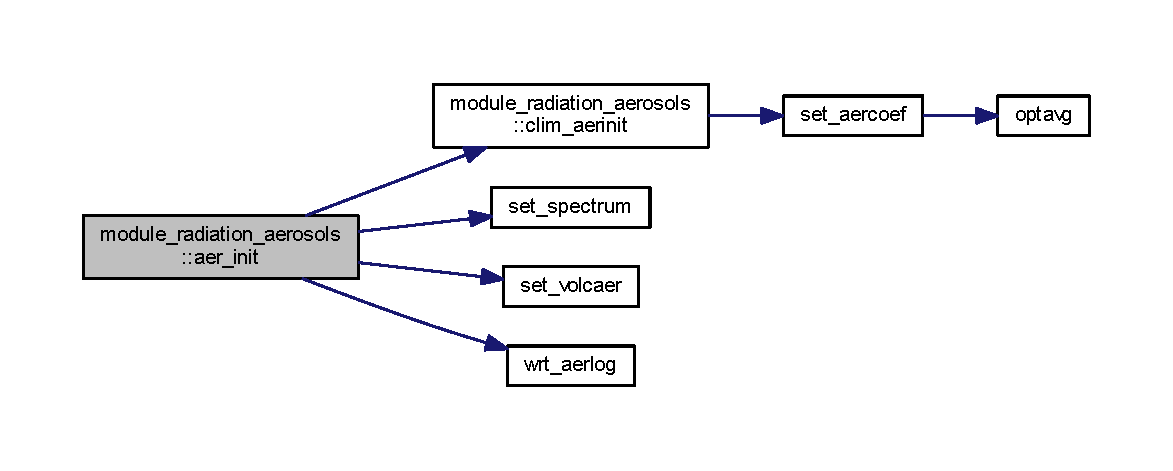
\includegraphics[width=350pt]{group__module__radiation__aerosols_gabe52f1b6f62b158154e70a7b5058ad20_cgraph}
\end{center}
\end{figure}




Here is the caller graph for this function\+:
\nopagebreak
\begin{figure}[H]
\begin{center}
\leavevmode
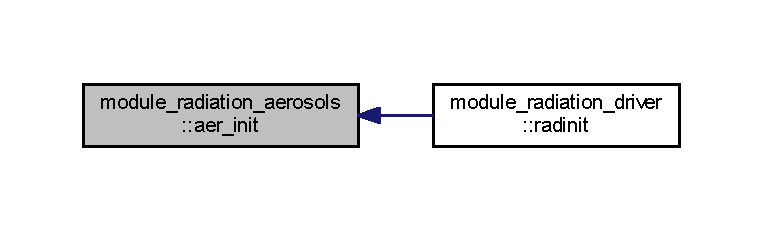
\includegraphics[width=350pt]{group__module__radiation__aerosols_gabe52f1b6f62b158154e70a7b5058ad20_icgraph}
\end{center}
\end{figure}


\index{module\+\_\+radiation\+\_\+aerosols@{module\+\_\+radiation\+\_\+aerosols}!aer\+\_\+property@{aer\+\_\+property}}
\index{aer\+\_\+property@{aer\+\_\+property}!module\+\_\+radiation\+\_\+aerosols@{module\+\_\+radiation\+\_\+aerosols}}
\subsubsection[{\texorpdfstring{aer\+\_\+property}{aer_property}}]{\setlength{\rightskip}{0pt plus 5cm}subroutine module\+\_\+radiation\+\_\+aerosols\+::aer\+\_\+property (
\begin{DoxyParamCaption}
{}
\end{DoxyParamCaption}
)\hspace{0.3cm}{\ttfamily [private]}}\hypertarget{group__module__radiation__aerosols_ga021aee92f6c64f78fc11e26d5b2288cf}{}\label{group__module__radiation__aerosols_ga021aee92f6c64f78fc11e26d5b2288cf}

\begin{DoxyParams}[1]{Parameters}
\mbox{\tt in}  & {\em prsi} & real, (I\+M\+AX,N\+L\+P1), pressure at interface in mb \\
\hline
\mbox{\tt in}  & {\em prsl} & real, (I\+M\+AX,N\+L\+AY), layer mean pressure(not used) \\
\hline
\mbox{\tt in}  & {\em prslk} & real, (I\+M\+AX,N\+L\+AY), exner function= $(p/p0)^{rocp}$ (not used) \\
\hline
\mbox{\tt in}  & {\em tvly} & real, (I\+M\+AX,N\+L\+AY), layer virtual temperature (not used) \\
\hline
\mbox{\tt in}  & {\em rhlay} & real, (I\+M\+AX,N\+L\+AY), layer mean relative humidity \\
\hline
\mbox{\tt in}  & {\em dz} & real, (I\+M\+AX,N\+L\+AY), layer thickness in m \\
\hline
\mbox{\tt in}  & {\em hz} & real, (I\+M\+AX,N\+L\+P1), level high in m \\
\hline
\mbox{\tt in}  & {\em tracer} & real, (I\+M\+AX,N\+L\+AY,N\+T\+R\+AC), aer tracer concentrations (not used) \\
\hline
\mbox{\tt in}  & {\em alon,alat} & real, (I\+M\+AX), longitude and latitude of given points in degree \\
\hline
\mbox{\tt in}  & {\em slmsk} & real, (I\+M\+AX), sea/land mask (sea\+:0,land\+:1,sea-\/ice\+:2) \\
\hline
\mbox{\tt in}  & {\em laersw,laerlw} & logical, 1, logical flag for sw/lw aerosol calculations \\
\hline
\mbox{\tt in}  & {\em I\+M\+AX} & integer, 1, horizontal dimension of arrays \\
\hline
\mbox{\tt in}  & {\em N\+L\+AY,N\+L\+P1} & integer, 1, vertical dimensions of arrays \\
\hline
\mbox{\tt in}  & {\em N\+S\+PC} & integer, 1, num of species for optional aod output fields \\
\hline
\mbox{\tt out}  & {\em aerosw} & real, (I\+M\+AX,N\+L\+AY,N\+B\+D\+SW,N\+F\+\_\+\+A\+E\+SW), aeros opt properties for sw ~\newline
 (\+:,\+:,\+:,1)\+: optical depth ~\newline
 (\+:,\+:,\+:,2)\+: single scattering albedo ~\newline
 (\+:,\+:,\+:,3)\+: asymmetry parameter \\
\hline
\mbox{\tt out}  & {\em aerolw} & real, (I\+M\+AX,N\+L\+AY,N\+B\+D\+LW,N\+F\+\_\+\+A\+E\+LW), aeros opt properties for lw ~\newline
 (\+:,\+:,\+:,1)\+: optical depth ~\newline
 (\+:,\+:,\+:,2)\+: single scattering albedo ~\newline
 (\+:,\+:,\+:,3)\+: asymmetry parameter \\
\hline
\mbox{\tt out}  & {\em aerodp} & real, (I\+M\+AX,N\+S\+P\+C+1), vertically integrated aer-\/opt-\/depth \\
\hline
\end{DoxyParams}

\begin{DoxyEnumerate}
\item Map aerosol data to model grids
\begin{DoxyItemize}
\item Map grid in longitude direction, lon from 0 to 355 deg resolution
\item Map grid in latitude direction, lat from 90n to 90s in 5 deg resolution
\end{DoxyItemize}
\item Determin the type of aerosol profile (kp) and scale hight for domain 1 (h1) to be used at this grid point
\item Compute horizontal bi-\/linear interpolation weights
\item Do horizontal bi-\/linear interpolation on aerosol partical density (denn)
\item Do horizontal bi-\/linear interpolation on mixing ratios
\item Prepare to setup domain index array and effective layer thickness. also convert pressure level to sigma level to follow the terrain
\item Call \hyperlink{group__module__radiation__aerosols_gae60b55ebc37825b2c3c95f95b23ed558}{radclimaer()} to calculate sw/lw aerosol optical properties for the corresponding frequency bands 
\end{DoxyEnumerate}

Definition at line 2603 of file radiation\+\_\+aerosols.\+f.



References cmixg, denng, f\+\_\+one, f\+\_\+zero, haer, idxcg, imxae, jmxae, kprfg, module\+\_\+radlw\+\_\+parameters\+::nbdlw, module\+\_\+radsw\+\_\+parameters\+::nbdsw, nlwbnd, nspc, nswbnd, nv\+\_\+aod, nxc, prsref, radclimaer(), and sigref.



Referenced by setaer().



Here is the call graph for this function\+:\nopagebreak
\begin{figure}[H]
\begin{center}
\leavevmode
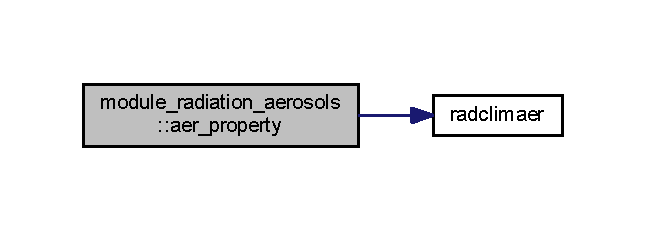
\includegraphics[width=310pt]{group__module__radiation__aerosols_ga021aee92f6c64f78fc11e26d5b2288cf_cgraph}
\end{center}
\end{figure}




Here is the caller graph for this function\+:
\nopagebreak
\begin{figure}[H]
\begin{center}
\leavevmode
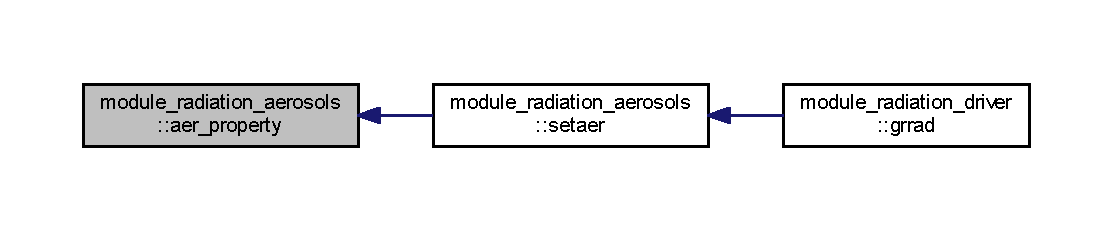
\includegraphics[width=350pt]{group__module__radiation__aerosols_ga021aee92f6c64f78fc11e26d5b2288cf_icgraph}
\end{center}
\end{figure}


\index{module\+\_\+radiation\+\_\+aerosols@{module\+\_\+radiation\+\_\+aerosols}!aer\+\_\+update@{aer\+\_\+update}}
\index{aer\+\_\+update@{aer\+\_\+update}!module\+\_\+radiation\+\_\+aerosols@{module\+\_\+radiation\+\_\+aerosols}}
\subsubsection[{\texorpdfstring{aer\+\_\+update}{aer_update}}]{\setlength{\rightskip}{0pt plus 5cm}subroutine, public module\+\_\+radiation\+\_\+aerosols\+::aer\+\_\+update (
\begin{DoxyParamCaption}
{}
\end{DoxyParamCaption}
)}\hypertarget{group__module__radiation__aerosols_ga1828b8076c7413903e66794b20ce1d37}{}\label{group__module__radiation__aerosols_ga1828b8076c7413903e66794b20ce1d37}

\begin{DoxyParams}[1]{Parameters}
\mbox{\tt in}  & {\em iyear} & integer, 1, 4-\/digit calender year \\
\hline
\mbox{\tt in}  & {\em imon} & integer, 1, month of the year \\
\hline
\mbox{\tt in}  & {\em me} & integer, 1, print message control flag \\
\hline
\mbox{\tt out}  & {\em N\+O\+NE} & \\
\hline
\end{DoxyParams}
\hypertarget{group__module__radsw__main_external}{}\subsection{External Module Variables}\label{group__module__radsw__main_external}
~\newline
 physparam\+::lalwflg -\/ control flag for tropospheric lw aerosol ~\newline
 physparam\+::laswflg -\/ control flag for tropospheric sw aerosol ~\newline
 physparam\+::lavoflg -\/ control flag for stratospheric volcanic aerosol \hypertarget{group__module__radiation__aerosols_subprograms}{}\subsection{Subprograms Called}\label{group__module__radiation__aerosols_subprograms}
~\newline
 -\/ trop\+\_\+update\+: This subprogram updates the monthly global distribution of aerosol profiles in five degree horizontal resolution. ~\newline
 -\/ volc\+\_\+update\+: This subprogram searches historical volcanic data sets to find and read in monthly 45-\/degree lat-\/zone band data of optical depth 

Definition at line 1649 of file radiation\+\_\+aerosols.\+f.



References trop\+\_\+update(), and volc\+\_\+update().



Referenced by module\+\_\+radiation\+\_\+driver\+::radupdate().



Here is the call graph for this function\+:
\nopagebreak
\begin{figure}[H]
\begin{center}
\leavevmode
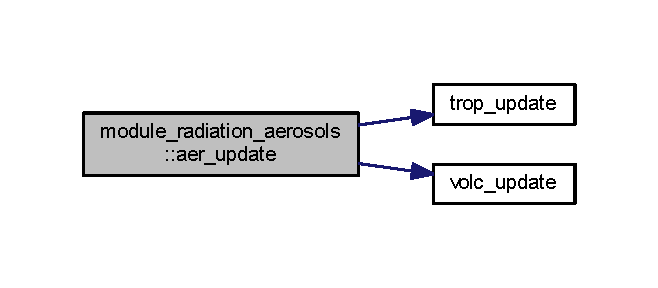
\includegraphics[width=316pt]{group__module__radiation__aerosols_ga1828b8076c7413903e66794b20ce1d37_cgraph}
\end{center}
\end{figure}




Here is the caller graph for this function\+:
\nopagebreak
\begin{figure}[H]
\begin{center}
\leavevmode
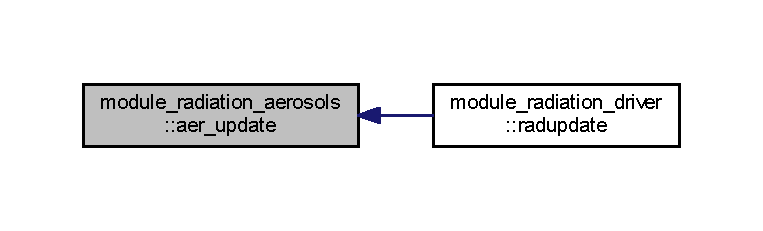
\includegraphics[width=350pt]{group__module__radiation__aerosols_ga1828b8076c7413903e66794b20ce1d37_icgraph}
\end{center}
\end{figure}


\index{module\+\_\+radiation\+\_\+aerosols@{module\+\_\+radiation\+\_\+aerosols}!aeropt\+\_\+grt@{aeropt\+\_\+grt}}
\index{aeropt\+\_\+grt@{aeropt\+\_\+grt}!module\+\_\+radiation\+\_\+aerosols@{module\+\_\+radiation\+\_\+aerosols}}
\subsubsection[{\texorpdfstring{aeropt\+\_\+grt}{aeropt_grt}}]{\setlength{\rightskip}{0pt plus 5cm}subroutine setgocartaer\+::aeropt\+\_\+grt (
\begin{DoxyParamCaption}
{}
\end{DoxyParamCaption}
)\hspace{0.3cm}{\ttfamily [private]}}\hypertarget{group__module__radiation__aerosols_ga4ff866c545425e7029a11999e97d8faa}{}\label{group__module__radiation__aerosols_ga4ff866c545425e7029a11999e97d8faa}


Definition at line 5058 of file radiation\+\_\+aerosols.\+f.



References asyrhd\+\_\+grt, asyrhi\+\_\+grt, dm\+\_\+indx, extrhd\+\_\+grt, extrhi\+\_\+grt, f\+\_\+one, f\+\_\+zero, gridcomp, isoot, issam, isuso, iwaso, kcm1, krhlev, max\+\_\+gridcomp, max\+\_\+num\+\_\+gridcomp, num\+\_\+gridcomp, nv\+\_\+aod, rhlev\+\_\+grt, ssarhd\+\_\+grt, and ssarhi\+\_\+grt.



Referenced by setgocartaer().



Here is the caller graph for this function\+:
\nopagebreak
\begin{figure}[H]
\begin{center}
\leavevmode
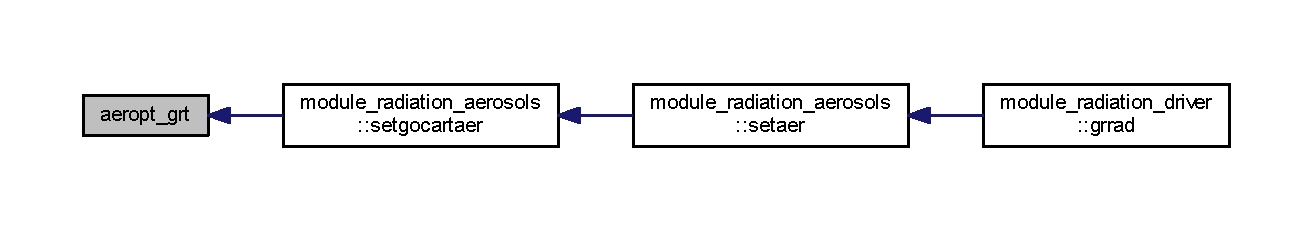
\includegraphics[width=350pt]{group__module__radiation__aerosols_ga4ff866c545425e7029a11999e97d8faa_icgraph}
\end{center}
\end{figure}


\index{module\+\_\+radiation\+\_\+aerosols@{module\+\_\+radiation\+\_\+aerosols}!clim\+\_\+aerinit@{clim\+\_\+aerinit}}
\index{clim\+\_\+aerinit@{clim\+\_\+aerinit}!module\+\_\+radiation\+\_\+aerosols@{module\+\_\+radiation\+\_\+aerosols}}
\subsubsection[{\texorpdfstring{clim\+\_\+aerinit}{clim_aerinit}}]{\setlength{\rightskip}{0pt plus 5cm}subroutine module\+\_\+radiation\+\_\+aerosols\+::clim\+\_\+aerinit (
\begin{DoxyParamCaption}
{}
\end{DoxyParamCaption}
)\hspace{0.3cm}{\ttfamily [private]}}\hypertarget{group__module__radiation__aerosols_ga0f5df46b558d8bd64f80161e83542222}{}\label{group__module__radiation__aerosols_ga0f5df46b558d8bd64f80161e83542222}

\begin{DoxyParams}[1]{Parameters}
\mbox{\tt in}  & {\em solfwv} & real, (N\+W\+V\+T\+OT), solar flux for each individual wavenumber $(w/m^2)$ \\
\hline
\mbox{\tt in}  & {\em eirfwv} & real, (N\+W\+V\+T\+IR), ir flux(273k) for each individual wavenum $(w/m^2)$ \\
\hline
\mbox{\tt in}  & {\em me} & integer, 1, print message control flag \\
\hline
\end{DoxyParams}


Definition at line 950 of file radiation\+\_\+aerosols.\+f.



References set\+\_\+aercoef().



Referenced by aer\+\_\+init().



Here is the call graph for this function\+:\nopagebreak
\begin{figure}[H]
\begin{center}
\leavevmode
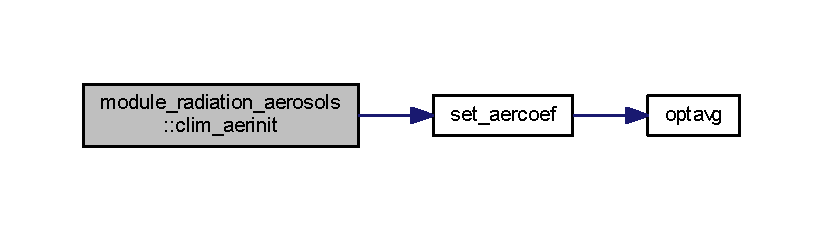
\includegraphics[width=350pt]{group__module__radiation__aerosols_ga0f5df46b558d8bd64f80161e83542222_cgraph}
\end{center}
\end{figure}




Here is the caller graph for this function\+:
\nopagebreak
\begin{figure}[H]
\begin{center}
\leavevmode
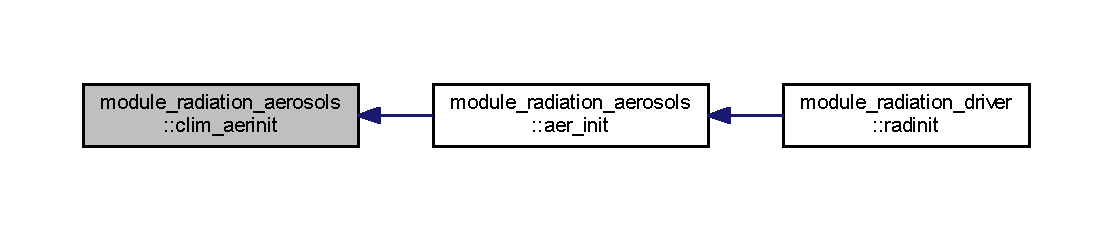
\includegraphics[width=350pt]{group__module__radiation__aerosols_ga0f5df46b558d8bd64f80161e83542222_icgraph}
\end{center}
\end{figure}


\index{module\+\_\+radiation\+\_\+aerosols@{module\+\_\+radiation\+\_\+aerosols}!gocart\+\_\+init@{gocart\+\_\+init}}
\index{gocart\+\_\+init@{gocart\+\_\+init}!module\+\_\+radiation\+\_\+aerosols@{module\+\_\+radiation\+\_\+aerosols}}
\subsubsection[{\texorpdfstring{gocart\+\_\+init}{gocart_init}}]{\setlength{\rightskip}{0pt plus 5cm}subroutine module\+\_\+radiation\+\_\+aerosols\+::gocart\+\_\+init (
\begin{DoxyParamCaption}
{}
\end{DoxyParamCaption}
)\hspace{0.3cm}{\ttfamily [private]}}\hypertarget{group__module__radiation__aerosols_gaed41923d67caaf1174eaa4303afdc55d}{}\label{group__module__radiation__aerosols_gaed41923d67caaf1174eaa4303afdc55d}

\begin{DoxyItemize}
\item determine weight and index for aerosol composition/luts
\item read in monthly global distribution of gocart aerosols
\item read and map the tabulated aerosol optical spectral data onto corresponding S\+W/\+LW radiation spectral bands. 
\end{DoxyItemize}

Definition at line 3365 of file radiation\+\_\+aerosols.\+f.



References extrhd\+\_\+grt, extrhi\+\_\+grt, f\+\_\+zero, get\+\_\+clim, iendwv\+\_\+grt, kaerbnd, krhlev, lckprnt, lgrtint, module\+\_\+radsw\+\_\+parameters\+::nbdsw, nlwbnd, nswlwbd, module\+\_\+radsw\+\_\+parameters\+::nswstr, nv\+\_\+aod, nwvtir, nwvtot, optavg\+\_\+grt(), rd\+\_\+gocart\+\_\+clim(), rd\+\_\+gocart\+\_\+luts(), rhdpasy0\+\_\+grt, rhdpext0\+\_\+grt, rhdpssa0\+\_\+grt, rhidasy0\+\_\+grt, rhidext0\+\_\+grt, rhidssa0\+\_\+grt, rhlev\+\_\+grt, set\+\_\+aerspc(), module\+\_\+radlw\+\_\+parameters\+::wvnlw1, and module\+\_\+radlw\+\_\+parameters\+::wvnlw2.



Here is the call graph for this function\+:\nopagebreak
\begin{figure}[H]
\begin{center}
\leavevmode
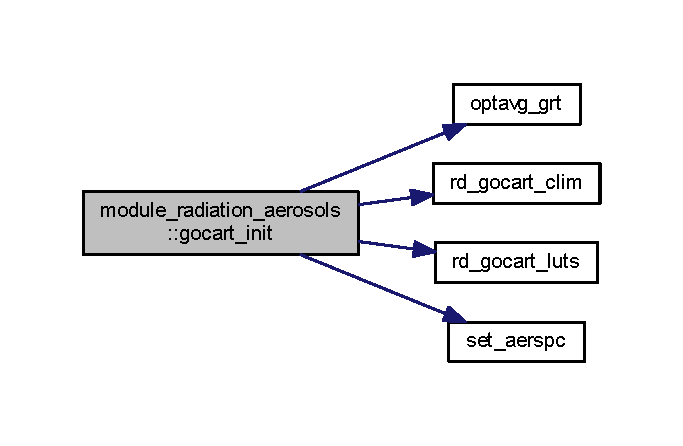
\includegraphics[width=328pt]{group__module__radiation__aerosols_gaed41923d67caaf1174eaa4303afdc55d_cgraph}
\end{center}
\end{figure}


\index{module\+\_\+radiation\+\_\+aerosols@{module\+\_\+radiation\+\_\+aerosols}!map\+\_\+aermr@{map\+\_\+aermr}}
\index{map\+\_\+aermr@{map\+\_\+aermr}!module\+\_\+radiation\+\_\+aerosols@{module\+\_\+radiation\+\_\+aerosols}}
\subsubsection[{\texorpdfstring{map\+\_\+aermr}{map_aermr}}]{\setlength{\rightskip}{0pt plus 5cm}subroutine setgocartaer\+::map\+\_\+aermr (
\begin{DoxyParamCaption}
{}
\end{DoxyParamCaption}
)\hspace{0.3cm}{\ttfamily [private]}}\hypertarget{group__module__radiation__aerosols_ga651c4be2fa354238990c5c7b9488e9fd}{}\label{group__module__radiation__aerosols_ga651c4be2fa354238990c5c7b9488e9fd}


Definition at line 4972 of file radiation\+\_\+aerosols.\+f.



References dm\+\_\+indx, dmfcs\+\_\+indx, and f\+\_\+zero.



Referenced by setgocartaer().



Here is the caller graph for this function\+:
\nopagebreak
\begin{figure}[H]
\begin{center}
\leavevmode
\includegraphics[width=350pt]{group__module__radiation__aerosols_ga651c4be2fa354238990c5c7b9488e9fd_icgraph}
\end{center}
\end{figure}


\index{module\+\_\+radiation\+\_\+aerosols@{module\+\_\+radiation\+\_\+aerosols}!optavg@{optavg}}
\index{optavg@{optavg}!module\+\_\+radiation\+\_\+aerosols@{module\+\_\+radiation\+\_\+aerosols}}
\subsubsection[{\texorpdfstring{optavg}{optavg}}]{\setlength{\rightskip}{0pt plus 5cm}subroutine clim\+\_\+aerinit\+::optavg (
\begin{DoxyParamCaption}
{}
\end{DoxyParamCaption}
)\hspace{0.3cm}{\ttfamily [private]}}\hypertarget{group__module__radiation__aerosols_ga637761b6110739f2d96322e2ddcc1291}{}\label{group__module__radiation__aerosols_ga637761b6110739f2d96322e2ddcc1291}


Definition at line 1375 of file radiation\+\_\+aerosols.\+f.



References asyrhd, asyrhi, extrhd, extrhi, extstra, f\+\_\+one, f\+\_\+zero, ncm1, ncm2, nlwbnd, nrhlev, nswbnd, scarhd, scarhi, ssarhd, and ssarhi.



Referenced by set\+\_\+aercoef().



Here is the caller graph for this function\+:
\nopagebreak
\begin{figure}[H]
\begin{center}
\leavevmode
\includegraphics[width=350pt]{group__module__radiation__aerosols_ga637761b6110739f2d96322e2ddcc1291_icgraph}
\end{center}
\end{figure}


\index{module\+\_\+radiation\+\_\+aerosols@{module\+\_\+radiation\+\_\+aerosols}!optavg\+\_\+grt@{optavg\+\_\+grt}}
\index{optavg\+\_\+grt@{optavg\+\_\+grt}!module\+\_\+radiation\+\_\+aerosols@{module\+\_\+radiation\+\_\+aerosols}}
\subsubsection[{\texorpdfstring{optavg\+\_\+grt}{optavg_grt}}]{\setlength{\rightskip}{0pt plus 5cm}subroutine gocart\+\_\+init\+::optavg\+\_\+grt (
\begin{DoxyParamCaption}
{}
\end{DoxyParamCaption}
)\hspace{0.3cm}{\ttfamily [private]}}\hypertarget{group__module__radiation__aerosols_ga8d1f5010e8cbc6abda50b8fc233ad7e9}{}\label{group__module__radiation__aerosols_ga8d1f5010e8cbc6abda50b8fc233ad7e9}


Definition at line 4155 of file radiation\+\_\+aerosols.\+f.



References asyrhd\+\_\+grt, asyrhi\+\_\+grt, extrhd\+\_\+grt, extrhi\+\_\+grt, f\+\_\+one, f\+\_\+zero, kcm1, kcm2, krhlev, rhdpasy0\+\_\+grt, rhdpext0\+\_\+grt, rhdpssa0\+\_\+grt, rhidasy0\+\_\+grt, rhidext0\+\_\+grt, rhidssa0\+\_\+grt, ssarhd\+\_\+grt, and ssarhi\+\_\+grt.



Referenced by gocart\+\_\+init().



Here is the caller graph for this function\+:
\nopagebreak
\begin{figure}[H]
\begin{center}
\leavevmode
\includegraphics[width=309pt]{group__module__radiation__aerosols_ga8d1f5010e8cbc6abda50b8fc233ad7e9_icgraph}
\end{center}
\end{figure}


\index{module\+\_\+radiation\+\_\+aerosols@{module\+\_\+radiation\+\_\+aerosols}!radclimaer@{radclimaer}}
\index{radclimaer@{radclimaer}!module\+\_\+radiation\+\_\+aerosols@{module\+\_\+radiation\+\_\+aerosols}}
\subsubsection[{\texorpdfstring{radclimaer}{radclimaer}}]{\setlength{\rightskip}{0pt plus 5cm}subroutine aer\+\_\+property\+::radclimaer (
\begin{DoxyParamCaption}
{}
\end{DoxyParamCaption}
)\hspace{0.3cm}{\ttfamily [private]}}\hypertarget{group__module__radiation__aerosols_gae60b55ebc37825b2c3c95f95b23ed558}{}\label{group__module__radiation__aerosols_gae60b55ebc37825b2c3c95f95b23ed558}

\begin{DoxyParams}[1]{Parameters}
\mbox{\tt in}  & {\em cmix} & real, (N\+CM), mixing ratioes of aerosol components \\
\hline
\mbox{\tt in}  & {\em denn} & real, 2, aerosol number densities \\
\hline
\mbox{\tt in}  & {\em rh1} & real, (N\+L\+AY), relative humidity \\
\hline
\mbox{\tt in}  & {\em delz} & real, (N\+L\+AY), effective layer thickness in km \\
\hline
\mbox{\tt in}  & {\em idmaer} & integer, (N\+L\+AY), aerosol domain index \\
\hline
\mbox{\tt in}  & {\em N\+XC} & integer, 1number of different aerosol components \\
\hline
\mbox{\tt in}  & {\em N\+L\+AY} & integer, 1, vertical dimensions \\
\hline
\mbox{\tt out}  & {\em tauae} & real, (N\+L\+AY, N\+S\+W\+L\+W\+BD), optical depth \\
\hline
\mbox{\tt out}  & {\em ssaae} & real, (N\+L\+AY, N\+S\+W\+L\+W\+BD), single scattering albedo \\
\hline
\mbox{\tt out}  & {\em asyae} & real, (N\+L\+AY, N\+S\+W\+L\+W\+BD), asymmetry parameter \\
\hline
\mbox{\tt out}  & {\em aerodp} & real, (I\+M\+AX, N\+S\+P\+C+1), vertically integrated aer-\/opt-\/depth \\
\hline
\end{DoxyParams}
\begin{DoxyRefDesc}{Todo}
\item[\hyperlink{todo__todo000001}{Todo}]radclimaer has no arguments; need to remove the parameter specifications above \end{DoxyRefDesc}


Definition at line 3051 of file radiation\+\_\+aerosols.\+f.



References asyrhd, asyrhi, extrhd, extrhi, extstra, f\+\_\+one, f\+\_\+zero, idxspc, ncm, ncm1, nrhlev, nswbnd, nswlwbd, nv\+\_\+aod, rhlev, scarhd, scarhi, ssarhd, and ssarhi.



Referenced by aer\+\_\+property().



Here is the caller graph for this function\+:
\nopagebreak
\begin{figure}[H]
\begin{center}
\leavevmode
\includegraphics[width=350pt]{group__module__radiation__aerosols_gae60b55ebc37825b2c3c95f95b23ed558_icgraph}
\end{center}
\end{figure}


\index{module\+\_\+radiation\+\_\+aerosols@{module\+\_\+radiation\+\_\+aerosols}!rd\+\_\+gocart\+\_\+clim@{rd\+\_\+gocart\+\_\+clim}}
\index{rd\+\_\+gocart\+\_\+clim@{rd\+\_\+gocart\+\_\+clim}!module\+\_\+radiation\+\_\+aerosols@{module\+\_\+radiation\+\_\+aerosols}}
\subsubsection[{\texorpdfstring{rd\+\_\+gocart\+\_\+clim}{rd_gocart_clim}}]{\setlength{\rightskip}{0pt plus 5cm}subroutine gocart\+\_\+init\+::rd\+\_\+gocart\+\_\+clim (
\begin{DoxyParamCaption}
{}
\end{DoxyParamCaption}
)\hspace{0.3cm}{\ttfamily [private]}}\hypertarget{group__module__radiation__aerosols_ga15bad8499ffd17d967e5788cd6721c4d}{}\label{group__module__radiation__aerosols_ga15bad8499ffd17d967e5788cd6721c4d}

\begin{DoxyEnumerate}
\item read in aerosol dry mass and surface pressure from G\+E\+O\+S3-\/\+G\+O\+C\+A\+RT C3.\+1 2000 monthly dataset or aerosol mixing ratio and surface pressure from G\+E\+O\+S4-\/\+G\+O\+C\+A\+RT 2000-\/2007 averaged monthly data set.
\item compute goes lat/lon array (for horizontal mapping) 
\end{DoxyEnumerate}

Definition at line 4373 of file radiation\+\_\+aerosols.\+f.



References dltx, dlty, dm\+\_\+indx, dmclmg, f\+\_\+zero, geos\+\_\+rlat, geos\+\_\+rlon, gocart\+\_\+climo, gridcomp, imxg, jmxg, kmxg, molwgt, nmxg, num\+\_\+gridcomp, and psclmg.



Referenced by gocart\+\_\+init().



Here is the caller graph for this function\+:
\nopagebreak
\begin{figure}[H]
\begin{center}
\leavevmode
\includegraphics[width=328pt]{group__module__radiation__aerosols_ga15bad8499ffd17d967e5788cd6721c4d_icgraph}
\end{center}
\end{figure}


\index{module\+\_\+radiation\+\_\+aerosols@{module\+\_\+radiation\+\_\+aerosols}!rd\+\_\+gocart\+\_\+luts@{rd\+\_\+gocart\+\_\+luts}}
\index{rd\+\_\+gocart\+\_\+luts@{rd\+\_\+gocart\+\_\+luts}!module\+\_\+radiation\+\_\+aerosols@{module\+\_\+radiation\+\_\+aerosols}}
\subsubsection[{\texorpdfstring{rd\+\_\+gocart\+\_\+luts}{rd_gocart_luts}}]{\setlength{\rightskip}{0pt plus 5cm}subroutine gocart\+\_\+init\+::rd\+\_\+gocart\+\_\+luts (
\begin{DoxyParamCaption}
{}
\end{DoxyParamCaption}
)\hspace{0.3cm}{\ttfamily [private]}}\hypertarget{group__module__radiation__aerosols_ga8b6a882f91674d1c0f7f71f297a5f92e}{}\label{group__module__radiation__aerosols_ga8b6a882f91674d1c0f7f71f297a5f92e}


Definition at line 3979 of file radiation\+\_\+aerosols.\+f.



References iendwv\+\_\+grt, isoot, issam, isscm, isuso, iwaso, kaerbnd, kcm1, kcm2, krhlev, lckprnt, rhdpasy0\+\_\+grt, rhdpext0\+\_\+grt, rhdpssa0\+\_\+grt, rhidasy0\+\_\+grt, rhidext0\+\_\+grt, and rhidssa0\+\_\+grt.



Referenced by gocart\+\_\+init().



Here is the caller graph for this function\+:
\nopagebreak
\begin{figure}[H]
\begin{center}
\leavevmode
\includegraphics[width=326pt]{group__module__radiation__aerosols_ga8b6a882f91674d1c0f7f71f297a5f92e_icgraph}
\end{center}
\end{figure}


\index{module\+\_\+radiation\+\_\+aerosols@{module\+\_\+radiation\+\_\+aerosols}!set\+\_\+aercoef@{set\+\_\+aercoef}}
\index{set\+\_\+aercoef@{set\+\_\+aercoef}!module\+\_\+radiation\+\_\+aerosols@{module\+\_\+radiation\+\_\+aerosols}}
\subsubsection[{\texorpdfstring{set\+\_\+aercoef}{set_aercoef}}]{\setlength{\rightskip}{0pt plus 5cm}subroutine clim\+\_\+aerinit\+::set\+\_\+aercoef (
\begin{DoxyParamCaption}
{}
\end{DoxyParamCaption}
)\hspace{0.3cm}{\ttfamily [private]}}\hypertarget{group__module__radiation__aerosols_ga95fabbc4272ae70f3b345f9b1a898d46}{}\label{group__module__radiation__aerosols_ga95fabbc4272ae70f3b345f9b1a898d46}


Definition at line 1038 of file radiation\+\_\+aerosols.\+f.



References asyrhd, asyrhi, extrhd, extrhi, extstra, f\+\_\+zero, haer, imxae, jmxae, naerbnd, ncm1, ncm2, nlwbnd, nlwstr, nrhlev, nswbnd, nswlwbd, module\+\_\+radsw\+\_\+parameters\+::nswstr, nv\+\_\+aod, optavg(), prsref, scarhd, scarhi, sigref, ssarhd, ssarhi, wvn550, module\+\_\+radlw\+\_\+parameters\+::wvnlw1, and module\+\_\+radlw\+\_\+parameters\+::wvnlw2.



Referenced by clim\+\_\+aerinit().



Here is the call graph for this function\+:\nopagebreak
\begin{figure}[H]
\begin{center}
\leavevmode
\includegraphics[width=227pt]{group__module__radiation__aerosols_ga95fabbc4272ae70f3b345f9b1a898d46_cgraph}
\end{center}
\end{figure}




Here is the caller graph for this function\+:
\nopagebreak
\begin{figure}[H]
\begin{center}
\leavevmode
\includegraphics[width=350pt]{group__module__radiation__aerosols_ga95fabbc4272ae70f3b345f9b1a898d46_icgraph}
\end{center}
\end{figure}


\index{module\+\_\+radiation\+\_\+aerosols@{module\+\_\+radiation\+\_\+aerosols}!set\+\_\+aerspc@{set\+\_\+aerspc}}
\index{set\+\_\+aerspc@{set\+\_\+aerspc}!module\+\_\+radiation\+\_\+aerosols@{module\+\_\+radiation\+\_\+aerosols}}
\subsubsection[{\texorpdfstring{set\+\_\+aerspc(raddt, fdaer)}{set_aerspc(raddt, fdaer)}}]{\setlength{\rightskip}{0pt plus 5cm}subroutine gocart\+\_\+init\+::set\+\_\+aerspc (
\begin{DoxyParamCaption}
\item[{real (kind=kind\+\_\+phys), intent(in)}]{raddt, }
\item[{real (kind=kind\+\_\+phys), intent(in)}]{fdaer}
\end{DoxyParamCaption}
)\hspace{0.3cm}{\ttfamily [private]}}\hypertarget{group__module__radiation__aerosols_gafb13b833ac59cf949702bdbde93d2c44}{}\label{group__module__radiation__aerosols_gafb13b833ac59cf949702bdbde93d2c44}


Definition at line 3680 of file radiation\+\_\+aerosols.\+f.



References ctaer, dm\+\_\+indx, dmfcs\+\_\+indx, f\+\_\+one, f\+\_\+zero, get\+\_\+clim, get\+\_\+fcst, gridcomp, isoot, issam, isscm, isuso, iwaso, kcm, kcm1, kcm2, lckprnt, max\+\_\+gridcomp, max\+\_\+num\+\_\+gridcomp, nmxg, and num\+\_\+gridcomp.



Referenced by gocart\+\_\+init().



Here is the caller graph for this function\+:
\nopagebreak
\begin{figure}[H]
\begin{center}
\leavevmode
\includegraphics[width=313pt]{group__module__radiation__aerosols_gafb13b833ac59cf949702bdbde93d2c44_icgraph}
\end{center}
\end{figure}


\index{module\+\_\+radiation\+\_\+aerosols@{module\+\_\+radiation\+\_\+aerosols}!set\+\_\+spectrum@{set\+\_\+spectrum}}
\index{set\+\_\+spectrum@{set\+\_\+spectrum}!module\+\_\+radiation\+\_\+aerosols@{module\+\_\+radiation\+\_\+aerosols}}
\subsubsection[{\texorpdfstring{set\+\_\+spectrum}{set_spectrum}}]{\setlength{\rightskip}{0pt plus 5cm}subroutine aer\+\_\+init\+::set\+\_\+spectrum (
\begin{DoxyParamCaption}
{}
\end{DoxyParamCaption}
)\hspace{0.3cm}{\ttfamily [private]}}\hypertarget{group__module__radiation__aerosols_gaa7fe6dc2964bc474a132b93aaab82cb0}{}\label{group__module__radiation__aerosols_gaa7fe6dc2964bc474a132b93aaab82cb0}


Definition at line 814 of file radiation\+\_\+aerosols.\+f.



References nwvns0, nwvsol, nwvtir, and s0intv.



Referenced by aer\+\_\+init().



Here is the caller graph for this function\+:
\nopagebreak
\begin{figure}[H]
\begin{center}
\leavevmode
\includegraphics[width=350pt]{group__module__radiation__aerosols_gaa7fe6dc2964bc474a132b93aaab82cb0_icgraph}
\end{center}
\end{figure}


\index{module\+\_\+radiation\+\_\+aerosols@{module\+\_\+radiation\+\_\+aerosols}!set\+\_\+volcaer@{set\+\_\+volcaer}}
\index{set\+\_\+volcaer@{set\+\_\+volcaer}!module\+\_\+radiation\+\_\+aerosols@{module\+\_\+radiation\+\_\+aerosols}}
\subsubsection[{\texorpdfstring{set\+\_\+volcaer}{set_volcaer}}]{\setlength{\rightskip}{0pt plus 5cm}subroutine aer\+\_\+init\+::set\+\_\+volcaer (
\begin{DoxyParamCaption}
{}
\end{DoxyParamCaption}
)\hspace{0.3cm}{\ttfamily [private]}}\hypertarget{group__module__radiation__aerosols_ga9b4558586df512eab092565549b835e2}{}\label{group__module__radiation__aerosols_ga9b4558586df512eab092565549b835e2}


Definition at line 903 of file radiation\+\_\+aerosols.\+f.



References ivolae.



Referenced by aer\+\_\+init().



Here is the caller graph for this function\+:
\nopagebreak
\begin{figure}[H]
\begin{center}
\leavevmode
\includegraphics[width=350pt]{group__module__radiation__aerosols_ga9b4558586df512eab092565549b835e2_icgraph}
\end{center}
\end{figure}


\index{module\+\_\+radiation\+\_\+aerosols@{module\+\_\+radiation\+\_\+aerosols}!setaer@{setaer}}
\index{setaer@{setaer}!module\+\_\+radiation\+\_\+aerosols@{module\+\_\+radiation\+\_\+aerosols}}
\subsubsection[{\texorpdfstring{setaer}{setaer}}]{\setlength{\rightskip}{0pt plus 5cm}subroutine, public module\+\_\+radiation\+\_\+aerosols\+::setaer (
\begin{DoxyParamCaption}
{}
\end{DoxyParamCaption}
)}\hypertarget{group__module__radiation__aerosols_ga559549bedb091683f71a705a875222d8}{}\label{group__module__radiation__aerosols_ga559549bedb091683f71a705a875222d8}

\begin{DoxyParams}[1]{Parameters}
\mbox{\tt in}  & {\em prsi} & (I\+M\+AX,N\+L\+P1), pressure at interface in mb \\
\hline
\mbox{\tt in}  & {\em prsl} & (I\+M\+AX,N\+L\+AY), layer mean pressure in mb \\
\hline
\mbox{\tt in}  & {\em prslk} & (I\+M\+AX,N\+L\+AY), exner function = $(p/p0)^{rocp}$ \\
\hline
\mbox{\tt in}  & {\em tvly} & (I\+M\+AX,N\+L\+AY), layer virtual temperature in K \\
\hline
\mbox{\tt in}  & {\em rhlay} & (I\+M\+AX,N\+L\+AY), layer mean relative humidity \\
\hline
\mbox{\tt in}  & {\em slmsk} & (I\+M\+AX), sea/land mask (sea\+:0,land\+:1,sea-\/ice\+:2) \\
\hline
\mbox{\tt in}  & {\em tracer} & (I\+M\+AX,N\+L\+AY,N\+T\+R\+AC), aerosol tracer concentration \\
\hline
\mbox{\tt in}  & {\em xlon} & (I\+M\+AX), longitude of given points in radiance, ok for both 0-\/$>$2pi or -\/pi-\/$>$+pi ranges \\
\hline
\mbox{\tt in}  & {\em xlat} & (I\+M\+AX), latitude of given points in radiance, default to pi/2 -\/$>$ -\/pi/2, otherwise see in-\/line comment \\
\hline
\mbox{\tt in}  & {\em I\+M\+AX} & 1, horizontal dimension of arrays \\
\hline
\mbox{\tt in}  & {\em N\+L\+AY,N\+L\+P1} & 1, vertical dimensions of arrays \\
\hline
\mbox{\tt in}  & {\em lsswr,lslwr} & logical flags for sw/lw radiation calls \\
\hline
\mbox{\tt out}  & {\em aerosw} & (I\+M\+AX,N\+L\+AY,N\+B\+D\+SW,N\+F\+\_\+\+A\+E\+SW), aeros opt properties for sw ~\newline
 (\+:,\+:,\+:,1)\+: optical depth ~\newline
 (\+:,\+:,\+:,2)\+: single scattering albedo ~\newline
 (\+:,\+:,\+:,3)\+: asymmetry parameter \\
\hline
\mbox{\tt out}  & {\em aerolw} & (I\+M\+AX,N\+L\+AY,N\+B\+D\+LW,N\+F\+\_\+\+A\+E\+LW), aeros opt properties for lw ~\newline
 (\+:,\+:,\+:,1)\+: optical depth ~\newline
 (\+:,\+:,\+:,2)\+: single scattering albedo ~\newline
 (\+:,\+:,\+:,3)\+: asymmetry parameter \\
\hline
\mbox{\tt out}  & {\em tau\+\_\+gocart} & (I\+M\+AX,N\+L\+AY,M\+A\+X\+\_\+\+N\+U\+M\+\_\+\+G\+R\+I\+D\+C\+O\+MP), 550nm aeros opt depth \\
\hline
\mbox{\tt out}  & {\em aerodp} & (I\+M\+AX,N\+S\+P\+C1), vertically integrated optical depth \\
\hline
\end{DoxyParams}
\hypertarget{group__module__radsw__main_general}{}\subsection{General Algorithm}\label{group__module__radsw__main_general}

\begin{DoxyEnumerate}
\item Convert lat/lon from radiance to degree
\item Compute level height and layer thickness
\item Calculate sw aerosol optical properties for the corresponding frequency bands
\begin{DoxyItemize}
\item if opac aerosol climatology is used, call \hyperlink{group__module__radiation__aerosols_ga021aee92f6c64f78fc11e26d5b2288cf}{aer\+\_\+property()}\+: this subroutine maps the 5 degree global climatological aerosol data set onto model grids, and compute aerosol optical properties for sw and lw radiations.
\item if gocart aerosol scheme is used, call \hyperlink{group__module__radiation__aerosols_ga685dc5ac4b7da2a375800bef712cbb8b}{setgocartaer()}\+: this subroutine computes sw + lw aerosol optical properties for gocart aerosol species (merged from fcst and clim fields)
\end{DoxyItemize}
\item Compute stratosphere volcanic forcing
\begin{DoxyItemize}
\item select data in 4 lat bands, interpolation at the boundaries
\item Find lower boundary of stratosphere\+: polar, fixed at 25000pa (250mb); tropic, fixed at 15000pa (150mb); mid-\/lat, interpolation
\item sw\+: add volcanic aerosol optical depth to the background value
\item Smoothing profile at boundary if needed
\item lw\+: add volcanic aerosol optical depth to the background value 
\end{DoxyItemize}
\end{DoxyEnumerate}

Definition at line 2018 of file radiation\+\_\+aerosols.\+f.



References aer\+\_\+property(), f\+\_\+one, f\+\_\+zero, ivolae, kmonsav, kyrsav, module\+\_\+radlw\+\_\+parameters\+::nbdlw, module\+\_\+radsw\+\_\+parameters\+::nbdsw, nf\+\_\+aelw, nf\+\_\+aesw, nlwbnd, nspc1, nswlwbd, module\+\_\+radsw\+\_\+parameters\+::nswstr, setgocartaer(), module\+\_\+radlw\+\_\+parameters\+::wvnlw1, and module\+\_\+radlw\+\_\+parameters\+::wvnlw2.



Referenced by module\+\_\+radiation\+\_\+driver\+::grrad().



Here is the call graph for this function\+:
\nopagebreak
\begin{figure}[H]
\begin{center}
\leavevmode
\includegraphics[width=350pt]{group__module__radiation__aerosols_ga559549bedb091683f71a705a875222d8_cgraph}
\end{center}
\end{figure}




Here is the caller graph for this function\+:
\nopagebreak
\begin{figure}[H]
\begin{center}
\leavevmode
\includegraphics[width=350pt]{group__module__radiation__aerosols_ga559549bedb091683f71a705a875222d8_icgraph}
\end{center}
\end{figure}


\index{module\+\_\+radiation\+\_\+aerosols@{module\+\_\+radiation\+\_\+aerosols}!setgocartaer@{setgocartaer}}
\index{setgocartaer@{setgocartaer}!module\+\_\+radiation\+\_\+aerosols@{module\+\_\+radiation\+\_\+aerosols}}
\subsubsection[{\texorpdfstring{setgocartaer}{setgocartaer}}]{\setlength{\rightskip}{0pt plus 5cm}subroutine module\+\_\+radiation\+\_\+aerosols\+::setgocartaer (
\begin{DoxyParamCaption}
{}
\end{DoxyParamCaption}
)\hspace{0.3cm}{\ttfamily [private]}}\hypertarget{group__module__radiation__aerosols_ga685dc5ac4b7da2a375800bef712cbb8b}{}\label{group__module__radiation__aerosols_ga685dc5ac4b7da2a375800bef712cbb8b}


Definition at line 4694 of file radiation\+\_\+aerosols.\+f.



References aeropt\+\_\+grt(), ctaer, dmclmg, f\+\_\+one, f\+\_\+zero, geos\+\_\+rlat, geos\+\_\+rlon, get\+\_\+clim, get\+\_\+fcst, gocart\+\_\+climo, imxg, jmxg, kmxg, map\+\_\+aermr(), molwgt, module\+\_\+radlw\+\_\+parameters\+::nbdlw, module\+\_\+radsw\+\_\+parameters\+::nbdsw, nlwbnd, nmxg, nswlwbd, and psclmg.



Referenced by setaer().



Here is the call graph for this function\+:\nopagebreak
\begin{figure}[H]
\begin{center}
\leavevmode
\includegraphics[width=313pt]{group__module__radiation__aerosols_ga685dc5ac4b7da2a375800bef712cbb8b_cgraph}
\end{center}
\end{figure}




Here is the caller graph for this function\+:
\nopagebreak
\begin{figure}[H]
\begin{center}
\leavevmode
\includegraphics[width=350pt]{group__module__radiation__aerosols_ga685dc5ac4b7da2a375800bef712cbb8b_icgraph}
\end{center}
\end{figure}


\index{module\+\_\+radiation\+\_\+aerosols@{module\+\_\+radiation\+\_\+aerosols}!trop\+\_\+update@{trop\+\_\+update}}
\index{trop\+\_\+update@{trop\+\_\+update}!module\+\_\+radiation\+\_\+aerosols@{module\+\_\+radiation\+\_\+aerosols}}
\subsubsection[{\texorpdfstring{trop\+\_\+update}{trop_update}}]{\setlength{\rightskip}{0pt plus 5cm}subroutine aer\+\_\+update\+::trop\+\_\+update (
\begin{DoxyParamCaption}
{}
\end{DoxyParamCaption}
)\hspace{0.3cm}{\ttfamily [private]}}\hypertarget{group__module__radiation__aerosols_gafac9a9c603c033c8511e8dbfe984f703}{}\label{group__module__radiation__aerosols_gafac9a9c603c033c8511e8dbfe984f703}


Definition at line 1708 of file radiation\+\_\+aerosols.\+f.



References cmixg, denng, f\+\_\+one, f\+\_\+zero, idxcg, imxae, jmxae, kprfg, and nxc.



Referenced by aer\+\_\+update().



Here is the caller graph for this function\+:
\nopagebreak
\begin{figure}[H]
\begin{center}
\leavevmode
\includegraphics[width=350pt]{group__module__radiation__aerosols_gafac9a9c603c033c8511e8dbfe984f703_icgraph}
\end{center}
\end{figure}


\index{module\+\_\+radiation\+\_\+aerosols@{module\+\_\+radiation\+\_\+aerosols}!volc\+\_\+update@{volc\+\_\+update}}
\index{volc\+\_\+update@{volc\+\_\+update}!module\+\_\+radiation\+\_\+aerosols@{module\+\_\+radiation\+\_\+aerosols}}
\subsubsection[{\texorpdfstring{volc\+\_\+update}{volc_update}}]{\setlength{\rightskip}{0pt plus 5cm}subroutine aer\+\_\+update\+::volc\+\_\+update (
\begin{DoxyParamCaption}
{}
\end{DoxyParamCaption}
)\hspace{0.3cm}{\ttfamily [private]}}\hypertarget{group__module__radiation__aerosols_ga6ec9bd68d45a5f2c6bb9997bdad420c3}{}\label{group__module__radiation__aerosols_ga6ec9bd68d45a5f2c6bb9997bdad420c3}


Definition at line 1866 of file radiation\+\_\+aerosols.\+f.



References ivolae, kmonsav, kyrend, kyrsav, kyrstr, maxvyr, and minvyr.



Referenced by aer\+\_\+update().



Here is the caller graph for this function\+:
\nopagebreak
\begin{figure}[H]
\begin{center}
\leavevmode
\includegraphics[width=350pt]{group__module__radiation__aerosols_ga6ec9bd68d45a5f2c6bb9997bdad420c3_icgraph}
\end{center}
\end{figure}


\index{module\+\_\+radiation\+\_\+aerosols@{module\+\_\+radiation\+\_\+aerosols}!wrt\+\_\+aerlog@{wrt\+\_\+aerlog}}
\index{wrt\+\_\+aerlog@{wrt\+\_\+aerlog}!module\+\_\+radiation\+\_\+aerosols@{module\+\_\+radiation\+\_\+aerosols}}
\subsubsection[{\texorpdfstring{wrt\+\_\+aerlog}{wrt_aerlog}}]{\setlength{\rightskip}{0pt plus 5cm}subroutine aer\+\_\+init\+::wrt\+\_\+aerlog (
\begin{DoxyParamCaption}
{}
\end{DoxyParamCaption}
)\hspace{0.3cm}{\ttfamily [private]}}\hypertarget{group__module__radiation__aerosols_ga3135fdf318002f9d56dd2d93225f4aac}{}\label{group__module__radiation__aerosols_ga3135fdf318002f9d56dd2d93225f4aac}


Definition at line 717 of file radiation\+\_\+aerosols.\+f.



References vtagaer.



Referenced by aer\+\_\+init().



Here is the caller graph for this function\+:
\nopagebreak
\begin{figure}[H]
\begin{center}
\leavevmode
\includegraphics[width=350pt]{group__module__radiation__aerosols_ga3135fdf318002f9d56dd2d93225f4aac_icgraph}
\end{center}
\end{figure}




\subsection{Variable Documentation}
\index{module\+\_\+radiation\+\_\+aerosols@{module\+\_\+radiation\+\_\+aerosols}!asyrhd@{asyrhd}}
\index{asyrhd@{asyrhd}!module\+\_\+radiation\+\_\+aerosols@{module\+\_\+radiation\+\_\+aerosols}}
\subsubsection[{\texorpdfstring{asyrhd}{asyrhd}}]{\setlength{\rightskip}{0pt plus 5cm}real (kind=kind\+\_\+phys), dimension(\+:,\+:,\+:), allocatable, save module\+\_\+radiation\+\_\+aerosols\+::asyrhd\hspace{0.3cm}{\ttfamily [private]}}\hypertarget{group__module__radiation__aerosols_ga090d37e62ba333db64e28bf89e89a08d}{}\label{group__module__radiation__aerosols_ga090d37e62ba333db64e28bf89e89a08d}


Definition at line 306 of file radiation\+\_\+aerosols.\+f.



Referenced by optavg(), radclimaer(), and set\+\_\+aercoef().

\index{module\+\_\+radiation\+\_\+aerosols@{module\+\_\+radiation\+\_\+aerosols}!asyrhd\+\_\+grt@{asyrhd\+\_\+grt}}
\index{asyrhd\+\_\+grt@{asyrhd\+\_\+grt}!module\+\_\+radiation\+\_\+aerosols@{module\+\_\+radiation\+\_\+aerosols}}
\subsubsection[{\texorpdfstring{asyrhd\+\_\+grt}{asyrhd_grt}}]{\setlength{\rightskip}{0pt plus 5cm}real (kind=kind\+\_\+phys), dimension(\+:,\+:,\+:), allocatable, save module\+\_\+radiation\+\_\+aerosols\+::asyrhd\+\_\+grt\hspace{0.3cm}{\ttfamily [private]}}\hypertarget{group__module__radiation__aerosols_ga2da45b8bd425415ca417f6590cc54da6}{}\label{group__module__radiation__aerosols_ga2da45b8bd425415ca417f6590cc54da6}


Definition at line 392 of file radiation\+\_\+aerosols.\+f.



Referenced by aeropt\+\_\+grt(), and optavg\+\_\+grt().

\index{module\+\_\+radiation\+\_\+aerosols@{module\+\_\+radiation\+\_\+aerosols}!asyrhi@{asyrhi}}
\index{asyrhi@{asyrhi}!module\+\_\+radiation\+\_\+aerosols@{module\+\_\+radiation\+\_\+aerosols}}
\subsubsection[{\texorpdfstring{asyrhi}{asyrhi}}]{\setlength{\rightskip}{0pt plus 5cm}real (kind=kind\+\_\+phys), dimension(\+:,\+:), allocatable, save module\+\_\+radiation\+\_\+aerosols\+::asyrhi\hspace{0.3cm}{\ttfamily [private]}}\hypertarget{group__module__radiation__aerosols_gaac2d735c117dd7d1e72264e611764f79}{}\label{group__module__radiation__aerosols_gaac2d735c117dd7d1e72264e611764f79}


Definition at line 304 of file radiation\+\_\+aerosols.\+f.



Referenced by optavg(), radclimaer(), and set\+\_\+aercoef().

\index{module\+\_\+radiation\+\_\+aerosols@{module\+\_\+radiation\+\_\+aerosols}!asyrhi\+\_\+grt@{asyrhi\+\_\+grt}}
\index{asyrhi\+\_\+grt@{asyrhi\+\_\+grt}!module\+\_\+radiation\+\_\+aerosols@{module\+\_\+radiation\+\_\+aerosols}}
\subsubsection[{\texorpdfstring{asyrhi\+\_\+grt}{asyrhi_grt}}]{\setlength{\rightskip}{0pt plus 5cm}real (kind=kind\+\_\+phys), dimension(\+:,\+:), allocatable, save module\+\_\+radiation\+\_\+aerosols\+::asyrhi\+\_\+grt\hspace{0.3cm}{\ttfamily [private]}}\hypertarget{group__module__radiation__aerosols_ga4b5f80817af9f2116618d6c8f0e194de}{}\label{group__module__radiation__aerosols_ga4b5f80817af9f2116618d6c8f0e194de}


Definition at line 390 of file radiation\+\_\+aerosols.\+f.



Referenced by aeropt\+\_\+grt(), and optavg\+\_\+grt().

\index{module\+\_\+radiation\+\_\+aerosols@{module\+\_\+radiation\+\_\+aerosols}!bcphilic@{bcphilic}}
\index{bcphilic@{bcphilic}!module\+\_\+radiation\+\_\+aerosols@{module\+\_\+radiation\+\_\+aerosols}}
\subsubsection[{\texorpdfstring{bcphilic}{bcphilic}}]{\setlength{\rightskip}{0pt plus 5cm}integer module\+\_\+radiation\+\_\+aerosols\+::tracer\+\_\+index\+\_\+type\+::bcphilic\hspace{0.3cm}{\ttfamily [private]}}\hypertarget{group__module__radiation__aerosols_ga776ae744bfaad492a1aeccf32864d1a0}{}\label{group__module__radiation__aerosols_ga776ae744bfaad492a1aeccf32864d1a0}


Definition at line 502 of file radiation\+\_\+aerosols.\+f.

\index{module\+\_\+radiation\+\_\+aerosols@{module\+\_\+radiation\+\_\+aerosols}!bcphobic@{bcphobic}}
\index{bcphobic@{bcphobic}!module\+\_\+radiation\+\_\+aerosols@{module\+\_\+radiation\+\_\+aerosols}}
\subsubsection[{\texorpdfstring{bcphobic}{bcphobic}}]{\setlength{\rightskip}{0pt plus 5cm}integer module\+\_\+radiation\+\_\+aerosols\+::tracer\+\_\+index\+\_\+type\+::bcphobic\hspace{0.3cm}{\ttfamily [private]}}\hypertarget{group__module__radiation__aerosols_ga4b1c1a1b44b5eb68ec19abb48e748fa0}{}\label{group__module__radiation__aerosols_ga4b1c1a1b44b5eb68ec19abb48e748fa0}


Definition at line 502 of file radiation\+\_\+aerosols.\+f.

\index{module\+\_\+radiation\+\_\+aerosols@{module\+\_\+radiation\+\_\+aerosols}!cmixg@{cmixg}}
\index{cmixg@{cmixg}!module\+\_\+radiation\+\_\+aerosols@{module\+\_\+radiation\+\_\+aerosols}}
\subsubsection[{\texorpdfstring{cmixg}{cmixg}}]{\setlength{\rightskip}{0pt plus 5cm}real (kind=kind\+\_\+phys), dimension(nxc,imxae,jmxae), save module\+\_\+radiation\+\_\+aerosols\+::cmixg\hspace{0.3cm}{\ttfamily [private]}}\hypertarget{group__module__radiation__aerosols_ga358c83599fb321a59c958e54d9f284d9}{}\label{group__module__radiation__aerosols_ga358c83599fb321a59c958e54d9f284d9}


Definition at line 318 of file radiation\+\_\+aerosols.\+f.



Referenced by aer\+\_\+property(), and trop\+\_\+update().

\index{module\+\_\+radiation\+\_\+aerosols@{module\+\_\+radiation\+\_\+aerosols}!ctaer@{ctaer}}
\index{ctaer@{ctaer}!module\+\_\+radiation\+\_\+aerosols@{module\+\_\+radiation\+\_\+aerosols}}
\subsubsection[{\texorpdfstring{ctaer}{ctaer}}]{\setlength{\rightskip}{0pt plus 5cm}real (kind=kind\+\_\+phys), save module\+\_\+radiation\+\_\+aerosols\+::ctaer = f\+\_\+zero\hspace{0.3cm}{\ttfamily [private]}}\hypertarget{group__module__radiation__aerosols_ga4b0aa142aee31c40361dadc390ccc68e}{}\label{group__module__radiation__aerosols_ga4b0aa142aee31c40361dadc390ccc68e}


Definition at line 457 of file radiation\+\_\+aerosols.\+f.



Referenced by set\+\_\+aerspc(), and setgocartaer().

\index{module\+\_\+radiation\+\_\+aerosols@{module\+\_\+radiation\+\_\+aerosols}!data@{data}}
\index{data@{data}!module\+\_\+radiation\+\_\+aerosols@{module\+\_\+radiation\+\_\+aerosols}}
\subsubsection[{\texorpdfstring{data}{data}}]{\setlength{\rightskip}{0pt plus 5cm}real (kind=kind\+\_\+phys), dimension(krhlev) module\+\_\+radiation\+\_\+aerosols\+::data\hspace{0.3cm}{\ttfamily [private]}}\hypertarget{group__module__radiation__aerosols_ga1248e740e53498ed7a06f7d475b1fb25}{}\label{group__module__radiation__aerosols_ga1248e740e53498ed7a06f7d475b1fb25}


Definition at line 338 of file radiation\+\_\+aerosols.\+f.

\index{module\+\_\+radiation\+\_\+aerosols@{module\+\_\+radiation\+\_\+aerosols}!denng@{denng}}
\index{denng@{denng}!module\+\_\+radiation\+\_\+aerosols@{module\+\_\+radiation\+\_\+aerosols}}
\subsubsection[{\texorpdfstring{denng}{denng}}]{\setlength{\rightskip}{0pt plus 5cm}real (kind=kind\+\_\+phys), dimension( 2 ,imxae,jmxae), save module\+\_\+radiation\+\_\+aerosols\+::denng\hspace{0.3cm}{\ttfamily [private]}}\hypertarget{group__module__radiation__aerosols_ga0ccc698bc870cb6ccbc1c2b64a3f45f6}{}\label{group__module__radiation__aerosols_ga0ccc698bc870cb6ccbc1c2b64a3f45f6}


Definition at line 319 of file radiation\+\_\+aerosols.\+f.



Referenced by aer\+\_\+property(), and trop\+\_\+update().

\index{module\+\_\+radiation\+\_\+aerosols@{module\+\_\+radiation\+\_\+aerosols}!dltx@{dltx}}
\index{dltx@{dltx}!module\+\_\+radiation\+\_\+aerosols@{module\+\_\+radiation\+\_\+aerosols}}
\subsubsection[{\texorpdfstring{dltx}{dltx}}]{\setlength{\rightskip}{0pt plus 5cm}real (kind=kind\+\_\+phys), parameter module\+\_\+radiation\+\_\+aerosols\+::dltx = 360.\+0 / float(I\+M\+XG)\hspace{0.3cm}{\ttfamily [private]}}\hypertarget{group__module__radiation__aerosols_ga084315fde4afcad23cd3aeb18a4d8a4e}{}\label{group__module__radiation__aerosols_ga084315fde4afcad23cd3aeb18a4d8a4e}


Definition at line 417 of file radiation\+\_\+aerosols.\+f.



Referenced by rd\+\_\+gocart\+\_\+clim().

\index{module\+\_\+radiation\+\_\+aerosols@{module\+\_\+radiation\+\_\+aerosols}!dlty@{dlty}}
\index{dlty@{dlty}!module\+\_\+radiation\+\_\+aerosols@{module\+\_\+radiation\+\_\+aerosols}}
\subsubsection[{\texorpdfstring{dlty}{dlty}}]{\setlength{\rightskip}{0pt plus 5cm}real (kind=kind\+\_\+phys), parameter module\+\_\+radiation\+\_\+aerosols\+::dlty = 180.\+0 / float(J\+M\+XG-\/1)\hspace{0.3cm}{\ttfamily [private]}}\hypertarget{group__module__radiation__aerosols_ga499bb3c75e9802c5ee7fd6cdb6660f7e}{}\label{group__module__radiation__aerosols_ga499bb3c75e9802c5ee7fd6cdb6660f7e}


Definition at line 418 of file radiation\+\_\+aerosols.\+f.



Referenced by rd\+\_\+gocart\+\_\+clim().

\index{module\+\_\+radiation\+\_\+aerosols@{module\+\_\+radiation\+\_\+aerosols}!dm\+\_\+indx@{dm\+\_\+indx}}
\index{dm\+\_\+indx@{dm\+\_\+indx}!module\+\_\+radiation\+\_\+aerosols@{module\+\_\+radiation\+\_\+aerosols}}
\subsubsection[{\texorpdfstring{dm\+\_\+indx}{dm_indx}}]{\setlength{\rightskip}{0pt plus 5cm}type (gocart\+\_\+index\+\_\+type), save module\+\_\+radiation\+\_\+aerosols\+::dm\+\_\+indx\hspace{0.3cm}{\ttfamily [private]}}\hypertarget{group__module__radiation__aerosols_ga70c58693c0aac6e4dbb6cf425fb0ce6a}{}\label{group__module__radiation__aerosols_ga70c58693c0aac6e4dbb6cf425fb0ce6a}


Definition at line 498 of file radiation\+\_\+aerosols.\+f.



Referenced by aeropt\+\_\+grt(), map\+\_\+aermr(), rd\+\_\+gocart\+\_\+clim(), and set\+\_\+aerspc().

\index{module\+\_\+radiation\+\_\+aerosols@{module\+\_\+radiation\+\_\+aerosols}!dmclmg@{dmclmg}}
\index{dmclmg@{dmclmg}!module\+\_\+radiation\+\_\+aerosols@{module\+\_\+radiation\+\_\+aerosols}}
\subsubsection[{\texorpdfstring{dmclmg}{dmclmg}}]{\setlength{\rightskip}{0pt plus 5cm}real (kind=kind\+\_\+phys), dimension(\+:,\+:,\+:,\+:), allocatable, save module\+\_\+radiation\+\_\+aerosols\+::dmclmg\hspace{0.3cm}{\ttfamily [private]}}\hypertarget{group__module__radiation__aerosols_ga123d552c7f98f7371565f4e2017efd45}{}\label{group__module__radiation__aerosols_ga123d552c7f98f7371565f4e2017efd45}


Definition at line 426 of file radiation\+\_\+aerosols.\+f.



Referenced by rd\+\_\+gocart\+\_\+clim(), and setgocartaer().

\index{module\+\_\+radiation\+\_\+aerosols@{module\+\_\+radiation\+\_\+aerosols}!dmfcs\+\_\+indx@{dmfcs\+\_\+indx}}
\index{dmfcs\+\_\+indx@{dmfcs\+\_\+indx}!module\+\_\+radiation\+\_\+aerosols@{module\+\_\+radiation\+\_\+aerosols}}
\subsubsection[{\texorpdfstring{dmfcs\+\_\+indx}{dmfcs_indx}}]{\setlength{\rightskip}{0pt plus 5cm}type (tracer\+\_\+index\+\_\+type), save module\+\_\+radiation\+\_\+aerosols\+::dmfcs\+\_\+indx\hspace{0.3cm}{\ttfamily [private]}}\hypertarget{group__module__radiation__aerosols_gad6c4782fbaae13df20891197b67568ec}{}\label{group__module__radiation__aerosols_gad6c4782fbaae13df20891197b67568ec}


Definition at line 508 of file radiation\+\_\+aerosols.\+f.



Referenced by map\+\_\+aermr(), and set\+\_\+aerspc().

\index{module\+\_\+radiation\+\_\+aerosols@{module\+\_\+radiation\+\_\+aerosols}!du001@{du001}}
\index{du001@{du001}!module\+\_\+radiation\+\_\+aerosols@{module\+\_\+radiation\+\_\+aerosols}}
\subsubsection[{\texorpdfstring{du001}{du001}}]{\setlength{\rightskip}{0pt plus 5cm}integer module\+\_\+radiation\+\_\+aerosols\+::tracer\+\_\+index\+\_\+type\+::du001\hspace{0.3cm}{\ttfamily [private]}}\hypertarget{group__module__radiation__aerosols_gaf4355efd112704adbaeab5a3fd1d7912}{}\label{group__module__radiation__aerosols_gaf4355efd112704adbaeab5a3fd1d7912}


Definition at line 502 of file radiation\+\_\+aerosols.\+f.

\index{module\+\_\+radiation\+\_\+aerosols@{module\+\_\+radiation\+\_\+aerosols}!du002@{du002}}
\index{du002@{du002}!module\+\_\+radiation\+\_\+aerosols@{module\+\_\+radiation\+\_\+aerosols}}
\subsubsection[{\texorpdfstring{du002}{du002}}]{\setlength{\rightskip}{0pt plus 5cm}integer module\+\_\+radiation\+\_\+aerosols\+::tracer\+\_\+index\+\_\+type\+::du002\hspace{0.3cm}{\ttfamily [private]}}\hypertarget{group__module__radiation__aerosols_gab68920703fa2cda7cbc42cb568a2ed56}{}\label{group__module__radiation__aerosols_gab68920703fa2cda7cbc42cb568a2ed56}


Definition at line 502 of file radiation\+\_\+aerosols.\+f.

\index{module\+\_\+radiation\+\_\+aerosols@{module\+\_\+radiation\+\_\+aerosols}!du003@{du003}}
\index{du003@{du003}!module\+\_\+radiation\+\_\+aerosols@{module\+\_\+radiation\+\_\+aerosols}}
\subsubsection[{\texorpdfstring{du003}{du003}}]{\setlength{\rightskip}{0pt plus 5cm}integer module\+\_\+radiation\+\_\+aerosols\+::tracer\+\_\+index\+\_\+type\+::du003\hspace{0.3cm}{\ttfamily [private]}}\hypertarget{group__module__radiation__aerosols_ga9b2422518e2c8aaba9f0b64bd0c4676a}{}\label{group__module__radiation__aerosols_ga9b2422518e2c8aaba9f0b64bd0c4676a}


Definition at line 502 of file radiation\+\_\+aerosols.\+f.

\index{module\+\_\+radiation\+\_\+aerosols@{module\+\_\+radiation\+\_\+aerosols}!du004@{du004}}
\index{du004@{du004}!module\+\_\+radiation\+\_\+aerosols@{module\+\_\+radiation\+\_\+aerosols}}
\subsubsection[{\texorpdfstring{du004}{du004}}]{\setlength{\rightskip}{0pt plus 5cm}integer module\+\_\+radiation\+\_\+aerosols\+::tracer\+\_\+index\+\_\+type\+::du004\hspace{0.3cm}{\ttfamily [private]}}\hypertarget{group__module__radiation__aerosols_ga69658f70ffccecfae1751c227ec1b14c}{}\label{group__module__radiation__aerosols_ga69658f70ffccecfae1751c227ec1b14c}


Definition at line 502 of file radiation\+\_\+aerosols.\+f.

\index{module\+\_\+radiation\+\_\+aerosols@{module\+\_\+radiation\+\_\+aerosols}!du005@{du005}}
\index{du005@{du005}!module\+\_\+radiation\+\_\+aerosols@{module\+\_\+radiation\+\_\+aerosols}}
\subsubsection[{\texorpdfstring{du005}{du005}}]{\setlength{\rightskip}{0pt plus 5cm}integer module\+\_\+radiation\+\_\+aerosols\+::tracer\+\_\+index\+\_\+type\+::du005\hspace{0.3cm}{\ttfamily [private]}}\hypertarget{group__module__radiation__aerosols_gaabd67af89106955952b0010bb3a70e4e}{}\label{group__module__radiation__aerosols_gaabd67af89106955952b0010bb3a70e4e}


Definition at line 502 of file radiation\+\_\+aerosols.\+f.

\index{module\+\_\+radiation\+\_\+aerosols@{module\+\_\+radiation\+\_\+aerosols}!dust1@{dust1}}
\index{dust1@{dust1}!module\+\_\+radiation\+\_\+aerosols@{module\+\_\+radiation\+\_\+aerosols}}
\subsubsection[{\texorpdfstring{dust1}{dust1}}]{\setlength{\rightskip}{0pt plus 5cm}integer module\+\_\+radiation\+\_\+aerosols\+::gocart\+\_\+index\+\_\+type\+::dust1\hspace{0.3cm}{\ttfamily [private]}}\hypertarget{group__module__radiation__aerosols_gae87b7754284ce0d44cab3ab11c7d302d}{}\label{group__module__radiation__aerosols_gae87b7754284ce0d44cab3ab11c7d302d}


Definition at line 492 of file radiation\+\_\+aerosols.\+f.

\index{module\+\_\+radiation\+\_\+aerosols@{module\+\_\+radiation\+\_\+aerosols}!dust2@{dust2}}
\index{dust2@{dust2}!module\+\_\+radiation\+\_\+aerosols@{module\+\_\+radiation\+\_\+aerosols}}
\subsubsection[{\texorpdfstring{dust2}{dust2}}]{\setlength{\rightskip}{0pt plus 5cm}integer module\+\_\+radiation\+\_\+aerosols\+::gocart\+\_\+index\+\_\+type\+::dust2\hspace{0.3cm}{\ttfamily [private]}}\hypertarget{group__module__radiation__aerosols_gaaf95cb5b3df728ac3b333edd8ab7820f}{}\label{group__module__radiation__aerosols_gaaf95cb5b3df728ac3b333edd8ab7820f}


Definition at line 492 of file radiation\+\_\+aerosols.\+f.

\index{module\+\_\+radiation\+\_\+aerosols@{module\+\_\+radiation\+\_\+aerosols}!dust3@{dust3}}
\index{dust3@{dust3}!module\+\_\+radiation\+\_\+aerosols@{module\+\_\+radiation\+\_\+aerosols}}
\subsubsection[{\texorpdfstring{dust3}{dust3}}]{\setlength{\rightskip}{0pt plus 5cm}integer module\+\_\+radiation\+\_\+aerosols\+::gocart\+\_\+index\+\_\+type\+::dust3\hspace{0.3cm}{\ttfamily [private]}}\hypertarget{group__module__radiation__aerosols_ga5d844db6dd6100b45808b5e19b468a84}{}\label{group__module__radiation__aerosols_ga5d844db6dd6100b45808b5e19b468a84}


Definition at line 492 of file radiation\+\_\+aerosols.\+f.

\index{module\+\_\+radiation\+\_\+aerosols@{module\+\_\+radiation\+\_\+aerosols}!dust4@{dust4}}
\index{dust4@{dust4}!module\+\_\+radiation\+\_\+aerosols@{module\+\_\+radiation\+\_\+aerosols}}
\subsubsection[{\texorpdfstring{dust4}{dust4}}]{\setlength{\rightskip}{0pt plus 5cm}integer module\+\_\+radiation\+\_\+aerosols\+::gocart\+\_\+index\+\_\+type\+::dust4\hspace{0.3cm}{\ttfamily [private]}}\hypertarget{group__module__radiation__aerosols_ga26a20aa03ac34523cc19644000d4924e}{}\label{group__module__radiation__aerosols_ga26a20aa03ac34523cc19644000d4924e}


Definition at line 492 of file radiation\+\_\+aerosols.\+f.

\index{module\+\_\+radiation\+\_\+aerosols@{module\+\_\+radiation\+\_\+aerosols}!dust5@{dust5}}
\index{dust5@{dust5}!module\+\_\+radiation\+\_\+aerosols@{module\+\_\+radiation\+\_\+aerosols}}
\subsubsection[{\texorpdfstring{dust5}{dust5}}]{\setlength{\rightskip}{0pt plus 5cm}integer module\+\_\+radiation\+\_\+aerosols\+::gocart\+\_\+index\+\_\+type\+::dust5\hspace{0.3cm}{\ttfamily [private]}}\hypertarget{group__module__radiation__aerosols_ga7d24acaa59ee8524dd8eca8f91f740c6}{}\label{group__module__radiation__aerosols_ga7d24acaa59ee8524dd8eca8f91f740c6}


Definition at line 492 of file radiation\+\_\+aerosols.\+f.

\index{module\+\_\+radiation\+\_\+aerosols@{module\+\_\+radiation\+\_\+aerosols}!extrhd@{extrhd}}
\index{extrhd@{extrhd}!module\+\_\+radiation\+\_\+aerosols@{module\+\_\+radiation\+\_\+aerosols}}
\subsubsection[{\texorpdfstring{extrhd}{extrhd}}]{\setlength{\rightskip}{0pt plus 5cm}real (kind=kind\+\_\+phys), dimension(\+:,\+:,\+:), allocatable, save module\+\_\+radiation\+\_\+aerosols\+::extrhd\hspace{0.3cm}{\ttfamily [private]}}\hypertarget{group__module__radiation__aerosols_ga1c69f7b8ff0c98252e94def83dabfed4}{}\label{group__module__radiation__aerosols_ga1c69f7b8ff0c98252e94def83dabfed4}


Definition at line 306 of file radiation\+\_\+aerosols.\+f.



Referenced by optavg(), radclimaer(), and set\+\_\+aercoef().

\index{module\+\_\+radiation\+\_\+aerosols@{module\+\_\+radiation\+\_\+aerosols}!extrhd\+\_\+grt@{extrhd\+\_\+grt}}
\index{extrhd\+\_\+grt@{extrhd\+\_\+grt}!module\+\_\+radiation\+\_\+aerosols@{module\+\_\+radiation\+\_\+aerosols}}
\subsubsection[{\texorpdfstring{extrhd\+\_\+grt}{extrhd_grt}}]{\setlength{\rightskip}{0pt plus 5cm}real (kind=kind\+\_\+phys), dimension(\+:,\+:,\+:), allocatable, save module\+\_\+radiation\+\_\+aerosols\+::extrhd\+\_\+grt\hspace{0.3cm}{\ttfamily [private]}}\hypertarget{group__module__radiation__aerosols_ga07bfe1ada075519d1d3ceabe21b65a96}{}\label{group__module__radiation__aerosols_ga07bfe1ada075519d1d3ceabe21b65a96}


Definition at line 392 of file radiation\+\_\+aerosols.\+f.



Referenced by aeropt\+\_\+grt(), gocart\+\_\+init(), and optavg\+\_\+grt().

\index{module\+\_\+radiation\+\_\+aerosols@{module\+\_\+radiation\+\_\+aerosols}!extrhi@{extrhi}}
\index{extrhi@{extrhi}!module\+\_\+radiation\+\_\+aerosols@{module\+\_\+radiation\+\_\+aerosols}}
\subsubsection[{\texorpdfstring{extrhi}{extrhi}}]{\setlength{\rightskip}{0pt plus 5cm}real (kind=kind\+\_\+phys), dimension(\+:,\+:), allocatable, save module\+\_\+radiation\+\_\+aerosols\+::extrhi\hspace{0.3cm}{\ttfamily [private]}}\hypertarget{group__module__radiation__aerosols_ga40447f925f01790155c4d98ff8b0c04d}{}\label{group__module__radiation__aerosols_ga40447f925f01790155c4d98ff8b0c04d}


Definition at line 304 of file radiation\+\_\+aerosols.\+f.



Referenced by optavg(), radclimaer(), and set\+\_\+aercoef().

\index{module\+\_\+radiation\+\_\+aerosols@{module\+\_\+radiation\+\_\+aerosols}!extrhi\+\_\+grt@{extrhi\+\_\+grt}}
\index{extrhi\+\_\+grt@{extrhi\+\_\+grt}!module\+\_\+radiation\+\_\+aerosols@{module\+\_\+radiation\+\_\+aerosols}}
\subsubsection[{\texorpdfstring{extrhi\+\_\+grt}{extrhi_grt}}]{\setlength{\rightskip}{0pt plus 5cm}real (kind=kind\+\_\+phys), dimension(\+:,\+:), allocatable, save module\+\_\+radiation\+\_\+aerosols\+::extrhi\+\_\+grt\hspace{0.3cm}{\ttfamily [private]}}\hypertarget{group__module__radiation__aerosols_gacb7ff037be78e950ea42d956816c93d5}{}\label{group__module__radiation__aerosols_gacb7ff037be78e950ea42d956816c93d5}


Definition at line 390 of file radiation\+\_\+aerosols.\+f.



Referenced by aeropt\+\_\+grt(), gocart\+\_\+init(), and optavg\+\_\+grt().

\index{module\+\_\+radiation\+\_\+aerosols@{module\+\_\+radiation\+\_\+aerosols}!extstra@{extstra}}
\index{extstra@{extstra}!module\+\_\+radiation\+\_\+aerosols@{module\+\_\+radiation\+\_\+aerosols}}
\subsubsection[{\texorpdfstring{extstra}{extstra}}]{\setlength{\rightskip}{0pt plus 5cm}real (kind=kind\+\_\+phys), dimension(\+:), allocatable, save module\+\_\+radiation\+\_\+aerosols\+::extstra\hspace{0.3cm}{\ttfamily [private]}}\hypertarget{group__module__radiation__aerosols_gac0c59f22f472671cd86221cc1ed46c60}{}\label{group__module__radiation__aerosols_gac0c59f22f472671cd86221cc1ed46c60}


Definition at line 308 of file radiation\+\_\+aerosols.\+f.



Referenced by optavg(), radclimaer(), and set\+\_\+aercoef().

\index{module\+\_\+radiation\+\_\+aerosols@{module\+\_\+radiation\+\_\+aerosols}!f\+\_\+one@{f\+\_\+one}}
\index{f\+\_\+one@{f\+\_\+one}!module\+\_\+radiation\+\_\+aerosols@{module\+\_\+radiation\+\_\+aerosols}}
\subsubsection[{\texorpdfstring{f\+\_\+one}{f_one}}]{\setlength{\rightskip}{0pt plus 5cm}real (kind=kind\+\_\+phys), parameter module\+\_\+radiation\+\_\+aerosols\+::f\+\_\+one = 1.\+0\hspace{0.3cm}{\ttfamily [private]}}\hypertarget{group__module__radiation__aerosols_ga63babe7f9ec4ff6a0364993f4be3768e}{}\label{group__module__radiation__aerosols_ga63babe7f9ec4ff6a0364993f4be3768e}


Definition at line 163 of file radiation\+\_\+aerosols.\+f.



Referenced by aer\+\_\+property(), aeropt\+\_\+grt(), optavg(), optavg\+\_\+grt(), radclimaer(), set\+\_\+aerspc(), setaer(), setgocartaer(), and trop\+\_\+update().

\index{module\+\_\+radiation\+\_\+aerosols@{module\+\_\+radiation\+\_\+aerosols}!f\+\_\+zero@{f\+\_\+zero}}
\index{f\+\_\+zero@{f\+\_\+zero}!module\+\_\+radiation\+\_\+aerosols@{module\+\_\+radiation\+\_\+aerosols}}
\subsubsection[{\texorpdfstring{f\+\_\+zero}{f_zero}}]{\setlength{\rightskip}{0pt plus 5cm}real (kind=kind\+\_\+phys), parameter module\+\_\+radiation\+\_\+aerosols\+::f\+\_\+zero = 0.\+0\hspace{0.3cm}{\ttfamily [private]}}\hypertarget{group__module__radiation__aerosols_ga7db1adcf476a9a5532230aa11fcc3bb7}{}\label{group__module__radiation__aerosols_ga7db1adcf476a9a5532230aa11fcc3bb7}


Definition at line 162 of file radiation\+\_\+aerosols.\+f.



Referenced by aer\+\_\+property(), aeropt\+\_\+grt(), gocart\+\_\+init(), map\+\_\+aermr(), optavg(), optavg\+\_\+grt(), radclimaer(), rd\+\_\+gocart\+\_\+clim(), set\+\_\+aercoef(), set\+\_\+aerspc(), setaer(), setgocartaer(), and trop\+\_\+update().

\index{module\+\_\+radiation\+\_\+aerosols@{module\+\_\+radiation\+\_\+aerosols}!geos\+\_\+rlat@{geos\+\_\+rlat}}
\index{geos\+\_\+rlat@{geos\+\_\+rlat}!module\+\_\+radiation\+\_\+aerosols@{module\+\_\+radiation\+\_\+aerosols}}
\subsubsection[{\texorpdfstring{geos\+\_\+rlat}{geos_rlat}}]{\setlength{\rightskip}{0pt plus 5cm}real (kind=kind\+\_\+phys), dimension(\+:), allocatable, save module\+\_\+radiation\+\_\+aerosols\+::geos\+\_\+rlat\hspace{0.3cm}{\ttfamily [private]}}\hypertarget{group__module__radiation__aerosols_gaef43bfbd28ef9b87e8d6973ba7331a18}{}\label{group__module__radiation__aerosols_gaef43bfbd28ef9b87e8d6973ba7331a18}


Definition at line 430 of file radiation\+\_\+aerosols.\+f.



Referenced by rd\+\_\+gocart\+\_\+clim(), and setgocartaer().

\index{module\+\_\+radiation\+\_\+aerosols@{module\+\_\+radiation\+\_\+aerosols}!geos\+\_\+rlon@{geos\+\_\+rlon}}
\index{geos\+\_\+rlon@{geos\+\_\+rlon}!module\+\_\+radiation\+\_\+aerosols@{module\+\_\+radiation\+\_\+aerosols}}
\subsubsection[{\texorpdfstring{geos\+\_\+rlon}{geos_rlon}}]{\setlength{\rightskip}{0pt plus 5cm}real (kind=kind\+\_\+phys), dimension(\+:), allocatable, save module\+\_\+radiation\+\_\+aerosols\+::geos\+\_\+rlon\hspace{0.3cm}{\ttfamily [private]}}\hypertarget{group__module__radiation__aerosols_ga1a0e35ab33517e765898870b8b1ab1ad}{}\label{group__module__radiation__aerosols_ga1a0e35ab33517e765898870b8b1ab1ad}


Definition at line 430 of file radiation\+\_\+aerosols.\+f.



Referenced by rd\+\_\+gocart\+\_\+clim(), and setgocartaer().

\index{module\+\_\+radiation\+\_\+aerosols@{module\+\_\+radiation\+\_\+aerosols}!get\+\_\+clim@{get\+\_\+clim}}
\index{get\+\_\+clim@{get\+\_\+clim}!module\+\_\+radiation\+\_\+aerosols@{module\+\_\+radiation\+\_\+aerosols}}
\subsubsection[{\texorpdfstring{get\+\_\+clim}{get_clim}}]{\setlength{\rightskip}{0pt plus 5cm}logical, save module\+\_\+radiation\+\_\+aerosols\+::get\+\_\+clim = .true.\hspace{0.3cm}{\ttfamily [private]}}\hypertarget{group__module__radiation__aerosols_ga7fe1943010fe47c9d86ef4c993848459}{}\label{group__module__radiation__aerosols_ga7fe1943010fe47c9d86ef4c993848459}


Definition at line 461 of file radiation\+\_\+aerosols.\+f.



Referenced by gocart\+\_\+init(), set\+\_\+aerspc(), and setgocartaer().

\index{module\+\_\+radiation\+\_\+aerosols@{module\+\_\+radiation\+\_\+aerosols}!get\+\_\+fcst@{get\+\_\+fcst}}
\index{get\+\_\+fcst@{get\+\_\+fcst}!module\+\_\+radiation\+\_\+aerosols@{module\+\_\+radiation\+\_\+aerosols}}
\subsubsection[{\texorpdfstring{get\+\_\+fcst}{get_fcst}}]{\setlength{\rightskip}{0pt plus 5cm}logical, save module\+\_\+radiation\+\_\+aerosols\+::get\+\_\+fcst = .true.\hspace{0.3cm}{\ttfamily [private]}}\hypertarget{group__module__radiation__aerosols_ga36f851e49de5e1f7da38da5fa6ea445c}{}\label{group__module__radiation__aerosols_ga36f851e49de5e1f7da38da5fa6ea445c}


Definition at line 460 of file radiation\+\_\+aerosols.\+f.



Referenced by set\+\_\+aerspc(), and setgocartaer().

\index{module\+\_\+radiation\+\_\+aerosols@{module\+\_\+radiation\+\_\+aerosols}!gocart\+\_\+climo@{gocart\+\_\+climo}}
\index{gocart\+\_\+climo@{gocart\+\_\+climo}!module\+\_\+radiation\+\_\+aerosols@{module\+\_\+radiation\+\_\+aerosols}}
\subsubsection[{\texorpdfstring{gocart\+\_\+climo}{gocart_climo}}]{\setlength{\rightskip}{0pt plus 5cm}character$\ast$4, save module\+\_\+radiation\+\_\+aerosols\+::gocart\+\_\+climo = \textquotesingle{}xxxx\textquotesingle{}\hspace{0.3cm}{\ttfamily [private]}}\hypertarget{group__module__radiation__aerosols_gab8118108e60a4795a8caa5af71232399}{}\label{group__module__radiation__aerosols_gab8118108e60a4795a8caa5af71232399}


Definition at line 435 of file radiation\+\_\+aerosols.\+f.



Referenced by rd\+\_\+gocart\+\_\+clim(), and setgocartaer().

\index{module\+\_\+radiation\+\_\+aerosols@{module\+\_\+radiation\+\_\+aerosols}!gridcomp@{gridcomp}}
\index{gridcomp@{gridcomp}!module\+\_\+radiation\+\_\+aerosols@{module\+\_\+radiation\+\_\+aerosols}}
\subsubsection[{\texorpdfstring{gridcomp}{gridcomp}}]{\setlength{\rightskip}{0pt plus 5cm}character, dimension(\+:), allocatable, save module\+\_\+radiation\+\_\+aerosols\+::gridcomp\hspace{0.3cm}{\ttfamily [private]}}\hypertarget{group__module__radiation__aerosols_ga48c2c6c9c509f5c37fea5d788040ad7a}{}\label{group__module__radiation__aerosols_ga48c2c6c9c509f5c37fea5d788040ad7a}


Definition at line 512 of file radiation\+\_\+aerosols.\+f.



Referenced by aeropt\+\_\+grt(), rd\+\_\+gocart\+\_\+clim(), and set\+\_\+aerspc().

\index{module\+\_\+radiation\+\_\+aerosols@{module\+\_\+radiation\+\_\+aerosols}!haer@{haer}}
\index{haer@{haer}!module\+\_\+radiation\+\_\+aerosols@{module\+\_\+radiation\+\_\+aerosols}}
\subsubsection[{\texorpdfstring{haer}{haer}}]{\setlength{\rightskip}{0pt plus 5cm}real (kind=kind\+\_\+phys), dimension(ndm,nae), save module\+\_\+radiation\+\_\+aerosols\+::haer\hspace{0.3cm}{\ttfamily [private]}}\hypertarget{group__module__radiation__aerosols_ga8ce24a58afb33dd372995bf5aaf95be9}{}\label{group__module__radiation__aerosols_ga8ce24a58afb33dd372995bf5aaf95be9}


Definition at line 281 of file radiation\+\_\+aerosols.\+f.



Referenced by aer\+\_\+property(), and set\+\_\+aercoef().

\index{module\+\_\+radiation\+\_\+aerosols@{module\+\_\+radiation\+\_\+aerosols}!idxcg@{idxcg}}
\index{idxcg@{idxcg}!module\+\_\+radiation\+\_\+aerosols@{module\+\_\+radiation\+\_\+aerosols}}
\subsubsection[{\texorpdfstring{idxcg}{idxcg}}]{\setlength{\rightskip}{0pt plus 5cm}integer, dimension(nxc,imxae,jmxae), save module\+\_\+radiation\+\_\+aerosols\+::idxcg\hspace{0.3cm}{\ttfamily [private]}}\hypertarget{group__module__radiation__aerosols_ga4cb38abaf6ece5a0ed717edd6f6b4078}{}\label{group__module__radiation__aerosols_ga4cb38abaf6ece5a0ed717edd6f6b4078}


Definition at line 320 of file radiation\+\_\+aerosols.\+f.



Referenced by aer\+\_\+property(), and trop\+\_\+update().

\index{module\+\_\+radiation\+\_\+aerosols@{module\+\_\+radiation\+\_\+aerosols}!idxspc@{idxspc}}
\index{idxspc@{idxspc}!module\+\_\+radiation\+\_\+aerosols@{module\+\_\+radiation\+\_\+aerosols}}
\subsubsection[{\texorpdfstring{idxspc}{idxspc}}]{\setlength{\rightskip}{0pt plus 5cm}integer, dimension(ncm) module\+\_\+radiation\+\_\+aerosols\+::idxspc\hspace{0.3cm}{\ttfamily [private]}}\hypertarget{group__module__radiation__aerosols_ga8ca79ca1e5161374aff3cad4121b360f}{}\label{group__module__radiation__aerosols_ga8ca79ca1e5161374aff3cad4121b360f}


Definition at line 531 of file radiation\+\_\+aerosols.\+f.



Referenced by radclimaer().

\index{module\+\_\+radiation\+\_\+aerosols@{module\+\_\+radiation\+\_\+aerosols}!iendwv\+\_\+grt@{iendwv\+\_\+grt}}
\index{iendwv\+\_\+grt@{iendwv\+\_\+grt}!module\+\_\+radiation\+\_\+aerosols@{module\+\_\+radiation\+\_\+aerosols}}
\subsubsection[{\texorpdfstring{iendwv\+\_\+grt}{iendwv_grt}}]{\setlength{\rightskip}{0pt plus 5cm}integer, dimension(\+:), allocatable module\+\_\+radiation\+\_\+aerosols\+::iendwv\+\_\+grt\hspace{0.3cm}{\ttfamily [private]}}\hypertarget{group__module__radiation__aerosols_gac755c4235327053fff060ffa3b2ee2a3}{}\label{group__module__radiation__aerosols_gac755c4235327053fff060ffa3b2ee2a3}


Definition at line 375 of file radiation\+\_\+aerosols.\+f.



Referenced by gocart\+\_\+init(), and rd\+\_\+gocart\+\_\+luts().

\index{module\+\_\+radiation\+\_\+aerosols@{module\+\_\+radiation\+\_\+aerosols}!imxae@{imxae}}
\index{imxae@{imxae}!module\+\_\+radiation\+\_\+aerosols@{module\+\_\+radiation\+\_\+aerosols}}
\subsubsection[{\texorpdfstring{imxae}{imxae}}]{\setlength{\rightskip}{0pt plus 5cm}integer, parameter module\+\_\+radiation\+\_\+aerosols\+::imxae = 72\hspace{0.3cm}{\ttfamily [private]}}\hypertarget{group__module__radiation__aerosols_ga52cda855a397136f75768d205292ddbb}{}\label{group__module__radiation__aerosols_ga52cda855a397136f75768d205292ddbb}


Definition at line 263 of file radiation\+\_\+aerosols.\+f.



Referenced by aer\+\_\+property(), set\+\_\+aercoef(), and trop\+\_\+update().

\index{module\+\_\+radiation\+\_\+aerosols@{module\+\_\+radiation\+\_\+aerosols}!imxg@{imxg}}
\index{imxg@{imxg}!module\+\_\+radiation\+\_\+aerosols@{module\+\_\+radiation\+\_\+aerosols}}
\subsubsection[{\texorpdfstring{imxg}{imxg}}]{\setlength{\rightskip}{0pt plus 5cm}integer, parameter module\+\_\+radiation\+\_\+aerosols\+::imxg = 144\hspace{0.3cm}{\ttfamily [private]}}\hypertarget{group__module__radiation__aerosols_gaa7b2e0e1d0669af4efc75cb32301f1f1}{}\label{group__module__radiation__aerosols_gaa7b2e0e1d0669af4efc75cb32301f1f1}


Definition at line 411 of file radiation\+\_\+aerosols.\+f.



Referenced by rd\+\_\+gocart\+\_\+clim(), and setgocartaer().

\index{module\+\_\+radiation\+\_\+aerosols@{module\+\_\+radiation\+\_\+aerosols}!isoot@{isoot}}
\index{isoot@{isoot}!module\+\_\+radiation\+\_\+aerosols@{module\+\_\+radiation\+\_\+aerosols}}
\subsubsection[{\texorpdfstring{isoot}{isoot}}]{\setlength{\rightskip}{0pt plus 5cm}integer, save module\+\_\+radiation\+\_\+aerosols\+::isoot\hspace{0.3cm}{\ttfamily [private]}}\hypertarget{group__module__radiation__aerosols_gaa9aa876f65d1e1e971607bff4ffbddad}{}\label{group__module__radiation__aerosols_gaa9aa876f65d1e1e971607bff4ffbddad}


Definition at line 483 of file radiation\+\_\+aerosols.\+f.



Referenced by aeropt\+\_\+grt(), rd\+\_\+gocart\+\_\+luts(), and set\+\_\+aerspc().

\index{module\+\_\+radiation\+\_\+aerosols@{module\+\_\+radiation\+\_\+aerosols}!issam@{issam}}
\index{issam@{issam}!module\+\_\+radiation\+\_\+aerosols@{module\+\_\+radiation\+\_\+aerosols}}
\subsubsection[{\texorpdfstring{issam}{issam}}]{\setlength{\rightskip}{0pt plus 5cm}integer, save module\+\_\+radiation\+\_\+aerosols\+::issam\hspace{0.3cm}{\ttfamily [private]}}\hypertarget{group__module__radiation__aerosols_gab64435256571a80bbb577fc4f27b39ee}{}\label{group__module__radiation__aerosols_gab64435256571a80bbb577fc4f27b39ee}


Definition at line 483 of file radiation\+\_\+aerosols.\+f.



Referenced by aeropt\+\_\+grt(), rd\+\_\+gocart\+\_\+luts(), and set\+\_\+aerspc().

\index{module\+\_\+radiation\+\_\+aerosols@{module\+\_\+radiation\+\_\+aerosols}!isscm@{isscm}}
\index{isscm@{isscm}!module\+\_\+radiation\+\_\+aerosols@{module\+\_\+radiation\+\_\+aerosols}}
\subsubsection[{\texorpdfstring{isscm}{isscm}}]{\setlength{\rightskip}{0pt plus 5cm}integer, save module\+\_\+radiation\+\_\+aerosols\+::isscm\hspace{0.3cm}{\ttfamily [private]}}\hypertarget{group__module__radiation__aerosols_ga762cff73e22fefab8adf68d08d5c4df1}{}\label{group__module__radiation__aerosols_ga762cff73e22fefab8adf68d08d5c4df1}


Definition at line 483 of file radiation\+\_\+aerosols.\+f.



Referenced by rd\+\_\+gocart\+\_\+luts(), and set\+\_\+aerspc().

\index{module\+\_\+radiation\+\_\+aerosols@{module\+\_\+radiation\+\_\+aerosols}!isuso@{isuso}}
\index{isuso@{isuso}!module\+\_\+radiation\+\_\+aerosols@{module\+\_\+radiation\+\_\+aerosols}}
\subsubsection[{\texorpdfstring{isuso}{isuso}}]{\setlength{\rightskip}{0pt plus 5cm}integer, save module\+\_\+radiation\+\_\+aerosols\+::isuso\hspace{0.3cm}{\ttfamily [private]}}\hypertarget{group__module__radiation__aerosols_gacddb4dccea82201fd3b193c15c85ec78}{}\label{group__module__radiation__aerosols_gacddb4dccea82201fd3b193c15c85ec78}


Definition at line 483 of file radiation\+\_\+aerosols.\+f.



Referenced by aeropt\+\_\+grt(), rd\+\_\+gocart\+\_\+luts(), and set\+\_\+aerspc().

\index{module\+\_\+radiation\+\_\+aerosols@{module\+\_\+radiation\+\_\+aerosols}!ivolae@{ivolae}}
\index{ivolae@{ivolae}!module\+\_\+radiation\+\_\+aerosols@{module\+\_\+radiation\+\_\+aerosols}}
\subsubsection[{\texorpdfstring{ivolae}{ivolae}}]{\setlength{\rightskip}{0pt plus 5cm}integer, dimension(\+:,\+:,\+:), allocatable, save module\+\_\+radiation\+\_\+aerosols\+::ivolae\hspace{0.3cm}{\ttfamily [private]}}\hypertarget{group__module__radiation__aerosols_gab016f51c81a1157ee234dc82f8f114ee}{}\label{group__module__radiation__aerosols_gab016f51c81a1157ee234dc82f8f114ee}


Definition at line 249 of file radiation\+\_\+aerosols.\+f.



Referenced by set\+\_\+volcaer(), setaer(), and volc\+\_\+update().

\index{module\+\_\+radiation\+\_\+aerosols@{module\+\_\+radiation\+\_\+aerosols}!iwaso@{iwaso}}
\index{iwaso@{iwaso}!module\+\_\+radiation\+\_\+aerosols@{module\+\_\+radiation\+\_\+aerosols}}
\subsubsection[{\texorpdfstring{iwaso}{iwaso}}]{\setlength{\rightskip}{0pt plus 5cm}integer, save module\+\_\+radiation\+\_\+aerosols\+::iwaso\hspace{0.3cm}{\ttfamily [private]}}\hypertarget{group__module__radiation__aerosols_gad15292f4a185c28ad44687d95ef4d3a4}{}\label{group__module__radiation__aerosols_gad15292f4a185c28ad44687d95ef4d3a4}


Definition at line 483 of file radiation\+\_\+aerosols.\+f.



Referenced by aeropt\+\_\+grt(), rd\+\_\+gocart\+\_\+luts(), and set\+\_\+aerspc().

\index{module\+\_\+radiation\+\_\+aerosols@{module\+\_\+radiation\+\_\+aerosols}!jmxae@{jmxae}}
\index{jmxae@{jmxae}!module\+\_\+radiation\+\_\+aerosols@{module\+\_\+radiation\+\_\+aerosols}}
\subsubsection[{\texorpdfstring{jmxae}{jmxae}}]{\setlength{\rightskip}{0pt plus 5cm}integer, parameter module\+\_\+radiation\+\_\+aerosols\+::jmxae = 37\hspace{0.3cm}{\ttfamily [private]}}\hypertarget{group__module__radiation__aerosols_gafdfdd058364062349b02cec9c712ea80}{}\label{group__module__radiation__aerosols_gafdfdd058364062349b02cec9c712ea80}


Definition at line 264 of file radiation\+\_\+aerosols.\+f.



Referenced by aer\+\_\+property(), set\+\_\+aercoef(), and trop\+\_\+update().

\index{module\+\_\+radiation\+\_\+aerosols@{module\+\_\+radiation\+\_\+aerosols}!jmxg@{jmxg}}
\index{jmxg@{jmxg}!module\+\_\+radiation\+\_\+aerosols@{module\+\_\+radiation\+\_\+aerosols}}
\subsubsection[{\texorpdfstring{jmxg}{jmxg}}]{\setlength{\rightskip}{0pt plus 5cm}integer, parameter module\+\_\+radiation\+\_\+aerosols\+::jmxg = 91\hspace{0.3cm}{\ttfamily [private]}}\hypertarget{group__module__radiation__aerosols_ga816ee06781e63adf8752a9a67ab2da2d}{}\label{group__module__radiation__aerosols_ga816ee06781e63adf8752a9a67ab2da2d}


Definition at line 412 of file radiation\+\_\+aerosols.\+f.



Referenced by rd\+\_\+gocart\+\_\+clim(), and setgocartaer().

\index{module\+\_\+radiation\+\_\+aerosols@{module\+\_\+radiation\+\_\+aerosols}!kaerbnd@{kaerbnd}}
\index{kaerbnd@{kaerbnd}!module\+\_\+radiation\+\_\+aerosols@{module\+\_\+radiation\+\_\+aerosols}}
\subsubsection[{\texorpdfstring{kaerbnd}{kaerbnd}}]{\setlength{\rightskip}{0pt plus 5cm}integer, parameter module\+\_\+radiation\+\_\+aerosols\+::kaerbnd =61\hspace{0.3cm}{\ttfamily [private]}}\hypertarget{group__module__radiation__aerosols_gad345c77fc29d8b02de34990162645a66}{}\label{group__module__radiation__aerosols_gad345c77fc29d8b02de34990162645a66}


Definition at line 329 of file radiation\+\_\+aerosols.\+f.



Referenced by gocart\+\_\+init(), and rd\+\_\+gocart\+\_\+luts().

\index{module\+\_\+radiation\+\_\+aerosols@{module\+\_\+radiation\+\_\+aerosols}!kcm@{kcm}}
\index{kcm@{kcm}!module\+\_\+radiation\+\_\+aerosols@{module\+\_\+radiation\+\_\+aerosols}}
\subsubsection[{\texorpdfstring{kcm}{kcm}}]{\setlength{\rightskip}{0pt plus 5cm}integer, save module\+\_\+radiation\+\_\+aerosols\+::kcm\hspace{0.3cm}{\ttfamily [private]}}\hypertarget{group__module__radiation__aerosols_ga4816bc93b826ff2fad9ff0805ea39fd5}{}\label{group__module__radiation__aerosols_ga4816bc93b826ff2fad9ff0805ea39fd5}


Definition at line 336 of file radiation\+\_\+aerosols.\+f.



Referenced by set\+\_\+aerspc().

\index{module\+\_\+radiation\+\_\+aerosols@{module\+\_\+radiation\+\_\+aerosols}!kcm1@{kcm1}}
\index{kcm1@{kcm1}!module\+\_\+radiation\+\_\+aerosols@{module\+\_\+radiation\+\_\+aerosols}}
\subsubsection[{\texorpdfstring{kcm1}{kcm1}}]{\setlength{\rightskip}{0pt plus 5cm}integer, save module\+\_\+radiation\+\_\+aerosols\+::kcm1 = 0\hspace{0.3cm}{\ttfamily [private]}}\hypertarget{group__module__radiation__aerosols_ga92b09dd26cc321af3b5da0b1c310a588}{}\label{group__module__radiation__aerosols_ga92b09dd26cc321af3b5da0b1c310a588}


Definition at line 334 of file radiation\+\_\+aerosols.\+f.



Referenced by aeropt\+\_\+grt(), optavg\+\_\+grt(), rd\+\_\+gocart\+\_\+luts(), and set\+\_\+aerspc().

\index{module\+\_\+radiation\+\_\+aerosols@{module\+\_\+radiation\+\_\+aerosols}!kcm2@{kcm2}}
\index{kcm2@{kcm2}!module\+\_\+radiation\+\_\+aerosols@{module\+\_\+radiation\+\_\+aerosols}}
\subsubsection[{\texorpdfstring{kcm2}{kcm2}}]{\setlength{\rightskip}{0pt plus 5cm}integer, save module\+\_\+radiation\+\_\+aerosols\+::kcm2 = 0\hspace{0.3cm}{\ttfamily [private]}}\hypertarget{group__module__radiation__aerosols_gab2be28697a95bcec8d5cd8de7ebd4328}{}\label{group__module__radiation__aerosols_gab2be28697a95bcec8d5cd8de7ebd4328}


Definition at line 335 of file radiation\+\_\+aerosols.\+f.



Referenced by optavg\+\_\+grt(), rd\+\_\+gocart\+\_\+luts(), and set\+\_\+aerspc().

\index{module\+\_\+radiation\+\_\+aerosols@{module\+\_\+radiation\+\_\+aerosols}!kmonsav@{kmonsav}}
\index{kmonsav@{kmonsav}!module\+\_\+radiation\+\_\+aerosols@{module\+\_\+radiation\+\_\+aerosols}}
\subsubsection[{\texorpdfstring{kmonsav}{kmonsav}}]{\setlength{\rightskip}{0pt plus 5cm}integer module\+\_\+radiation\+\_\+aerosols\+::kmonsav\hspace{0.3cm}{\ttfamily [private]}}\hypertarget{group__module__radiation__aerosols_ga302ae8a5aa2b8fb08ad366ef124cee45}{}\label{group__module__radiation__aerosols_ga302ae8a5aa2b8fb08ad366ef124cee45}


Definition at line 252 of file radiation\+\_\+aerosols.\+f.



Referenced by aer\+\_\+init(), setaer(), and volc\+\_\+update().

\index{module\+\_\+radiation\+\_\+aerosols@{module\+\_\+radiation\+\_\+aerosols}!kmxg@{kmxg}}
\index{kmxg@{kmxg}!module\+\_\+radiation\+\_\+aerosols@{module\+\_\+radiation\+\_\+aerosols}}
\subsubsection[{\texorpdfstring{kmxg}{kmxg}}]{\setlength{\rightskip}{0pt plus 5cm}integer, parameter module\+\_\+radiation\+\_\+aerosols\+::kmxg = 30\hspace{0.3cm}{\ttfamily [private]}}\hypertarget{group__module__radiation__aerosols_ga5339e589d92fab8cbb310b84b6ca3d9e}{}\label{group__module__radiation__aerosols_ga5339e589d92fab8cbb310b84b6ca3d9e}


Definition at line 413 of file radiation\+\_\+aerosols.\+f.



Referenced by rd\+\_\+gocart\+\_\+clim(), and setgocartaer().

\index{module\+\_\+radiation\+\_\+aerosols@{module\+\_\+radiation\+\_\+aerosols}!kprfg@{kprfg}}
\index{kprfg@{kprfg}!module\+\_\+radiation\+\_\+aerosols@{module\+\_\+radiation\+\_\+aerosols}}
\subsubsection[{\texorpdfstring{kprfg}{kprfg}}]{\setlength{\rightskip}{0pt plus 5cm}integer, dimension(    imxae,jmxae), save module\+\_\+radiation\+\_\+aerosols\+::kprfg\hspace{0.3cm}{\ttfamily [private]}}\hypertarget{group__module__radiation__aerosols_ga28df10ba381278cc7474bea0bfdaa870}{}\label{group__module__radiation__aerosols_ga28df10ba381278cc7474bea0bfdaa870}


Definition at line 321 of file radiation\+\_\+aerosols.\+f.



Referenced by aer\+\_\+property(), and trop\+\_\+update().

\index{module\+\_\+radiation\+\_\+aerosols@{module\+\_\+radiation\+\_\+aerosols}!krhlev@{krhlev}}
\index{krhlev@{krhlev}!module\+\_\+radiation\+\_\+aerosols@{module\+\_\+radiation\+\_\+aerosols}}
\subsubsection[{\texorpdfstring{krhlev}{krhlev}}]{\setlength{\rightskip}{0pt plus 5cm}integer, parameter module\+\_\+radiation\+\_\+aerosols\+::krhlev =36\hspace{0.3cm}{\ttfamily [private]}}\hypertarget{group__module__radiation__aerosols_ga33f2d4489a1730a27cbdc2e2add0f977}{}\label{group__module__radiation__aerosols_ga33f2d4489a1730a27cbdc2e2add0f977}


Definition at line 330 of file radiation\+\_\+aerosols.\+f.



Referenced by aeropt\+\_\+grt(), gocart\+\_\+init(), optavg\+\_\+grt(), and rd\+\_\+gocart\+\_\+luts().

\index{module\+\_\+radiation\+\_\+aerosols@{module\+\_\+radiation\+\_\+aerosols}!kyrend@{kyrend}}
\index{kyrend@{kyrend}!module\+\_\+radiation\+\_\+aerosols@{module\+\_\+radiation\+\_\+aerosols}}
\subsubsection[{\texorpdfstring{kyrend}{kyrend}}]{\setlength{\rightskip}{0pt plus 5cm}integer module\+\_\+radiation\+\_\+aerosols\+::kyrend\hspace{0.3cm}{\ttfamily [private]}}\hypertarget{group__module__radiation__aerosols_ga79127786cce93bccf8749ef8c85f6467}{}\label{group__module__radiation__aerosols_ga79127786cce93bccf8749ef8c85f6467}


Definition at line 252 of file radiation\+\_\+aerosols.\+f.



Referenced by aer\+\_\+init(), and volc\+\_\+update().

\index{module\+\_\+radiation\+\_\+aerosols@{module\+\_\+radiation\+\_\+aerosols}!kyrsav@{kyrsav}}
\index{kyrsav@{kyrsav}!module\+\_\+radiation\+\_\+aerosols@{module\+\_\+radiation\+\_\+aerosols}}
\subsubsection[{\texorpdfstring{kyrsav}{kyrsav}}]{\setlength{\rightskip}{0pt plus 5cm}integer module\+\_\+radiation\+\_\+aerosols\+::kyrsav\hspace{0.3cm}{\ttfamily [private]}}\hypertarget{group__module__radiation__aerosols_ga928c08857f866e4b848873a23a1d49e7}{}\label{group__module__radiation__aerosols_ga928c08857f866e4b848873a23a1d49e7}


Definition at line 252 of file radiation\+\_\+aerosols.\+f.



Referenced by aer\+\_\+init(), setaer(), and volc\+\_\+update().

\index{module\+\_\+radiation\+\_\+aerosols@{module\+\_\+radiation\+\_\+aerosols}!kyrstr@{kyrstr}}
\index{kyrstr@{kyrstr}!module\+\_\+radiation\+\_\+aerosols@{module\+\_\+radiation\+\_\+aerosols}}
\subsubsection[{\texorpdfstring{kyrstr}{kyrstr}}]{\setlength{\rightskip}{0pt plus 5cm}integer module\+\_\+radiation\+\_\+aerosols\+::kyrstr\hspace{0.3cm}{\ttfamily [private]}}\hypertarget{group__module__radiation__aerosols_gaf224f7d7991e3d48aeaa4d221da50f41}{}\label{group__module__radiation__aerosols_gaf224f7d7991e3d48aeaa4d221da50f41}


Definition at line 252 of file radiation\+\_\+aerosols.\+f.



Referenced by aer\+\_\+init(), and volc\+\_\+update().

\index{module\+\_\+radiation\+\_\+aerosols@{module\+\_\+radiation\+\_\+aerosols}!lckprnt@{lckprnt}}
\index{lckprnt@{lckprnt}!module\+\_\+radiation\+\_\+aerosols@{module\+\_\+radiation\+\_\+aerosols}}
\subsubsection[{\texorpdfstring{lckprnt}{lckprnt}}]{\setlength{\rightskip}{0pt plus 5cm}logical, save module\+\_\+radiation\+\_\+aerosols\+::lckprnt = .false.\hspace{0.3cm}{\ttfamily [private]}}\hypertarget{group__module__radiation__aerosols_ga018d5414597049069c1ddd1094285371}{}\label{group__module__radiation__aerosols_ga018d5414597049069c1ddd1094285371}


Definition at line 452 of file radiation\+\_\+aerosols.\+f.



Referenced by gocart\+\_\+init(), rd\+\_\+gocart\+\_\+luts(), and set\+\_\+aerspc().

\index{module\+\_\+radiation\+\_\+aerosols@{module\+\_\+radiation\+\_\+aerosols}!lgrtint@{lgrtint}}
\index{lgrtint@{lgrtint}!module\+\_\+radiation\+\_\+aerosols@{module\+\_\+radiation\+\_\+aerosols}}
\subsubsection[{\texorpdfstring{lgrtint}{lgrtint}}]{\setlength{\rightskip}{0pt plus 5cm}logical, save module\+\_\+radiation\+\_\+aerosols\+::lgrtint = .true.\hspace{0.3cm}{\ttfamily [private]}}\hypertarget{group__module__radiation__aerosols_gaa27bf6912bfd67b78381892d4f555c51}{}\label{group__module__radiation__aerosols_gaa27bf6912bfd67b78381892d4f555c51}


Definition at line 448 of file radiation\+\_\+aerosols.\+f.



Referenced by gocart\+\_\+init().

\index{module\+\_\+radiation\+\_\+aerosols@{module\+\_\+radiation\+\_\+aerosols}!max\+\_\+gridcomp@{max\+\_\+gridcomp}}
\index{max\+\_\+gridcomp@{max\+\_\+gridcomp}!module\+\_\+radiation\+\_\+aerosols@{module\+\_\+radiation\+\_\+aerosols}}
\subsubsection[{\texorpdfstring{max\+\_\+gridcomp}{max_gridcomp}}]{\setlength{\rightskip}{0pt plus 5cm}character$\ast$2, dimension(max\+\_\+num\+\_\+gridcomp) module\+\_\+radiation\+\_\+aerosols\+::max\+\_\+gridcomp\hspace{0.3cm}{\ttfamily [private]}}\hypertarget{group__module__radiation__aerosols_gac8278b0db773d6ba6ab4d71c9bb1b109}{}\label{group__module__radiation__aerosols_gac8278b0db773d6ba6ab4d71c9bb1b109}


Definition at line 516 of file radiation\+\_\+aerosols.\+f.



Referenced by aeropt\+\_\+grt(), and set\+\_\+aerspc().

\index{module\+\_\+radiation\+\_\+aerosols@{module\+\_\+radiation\+\_\+aerosols}!max\+\_\+num\+\_\+gridcomp@{max\+\_\+num\+\_\+gridcomp}}
\index{max\+\_\+num\+\_\+gridcomp@{max\+\_\+num\+\_\+gridcomp}!module\+\_\+radiation\+\_\+aerosols@{module\+\_\+radiation\+\_\+aerosols}}
\subsubsection[{\texorpdfstring{max\+\_\+num\+\_\+gridcomp}{max_num_gridcomp}}]{\setlength{\rightskip}{0pt plus 5cm}integer, parameter module\+\_\+radiation\+\_\+aerosols\+::max\+\_\+num\+\_\+gridcomp = 5\hspace{0.3cm}{\ttfamily [private]}}\hypertarget{group__module__radiation__aerosols_gad1187b5d87889c68cbe5929e20e83ac7}{}\label{group__module__radiation__aerosols_gad1187b5d87889c68cbe5929e20e83ac7}


Definition at line 515 of file radiation\+\_\+aerosols.\+f.



Referenced by aeropt\+\_\+grt(), and set\+\_\+aerspc().

\index{module\+\_\+radiation\+\_\+aerosols@{module\+\_\+radiation\+\_\+aerosols}!maxvyr@{maxvyr}}
\index{maxvyr@{maxvyr}!module\+\_\+radiation\+\_\+aerosols@{module\+\_\+radiation\+\_\+aerosols}}
\subsubsection[{\texorpdfstring{maxvyr}{maxvyr}}]{\setlength{\rightskip}{0pt plus 5cm}integer, parameter module\+\_\+radiation\+\_\+aerosols\+::maxvyr = 1999\hspace{0.3cm}{\ttfamily [private]}}\hypertarget{group__module__radiation__aerosols_gad856a3d564ff84043219626759673f27}{}\label{group__module__radiation__aerosols_gad856a3d564ff84043219626759673f27}


Definition at line 246 of file radiation\+\_\+aerosols.\+f.



Referenced by volc\+\_\+update().

\index{module\+\_\+radiation\+\_\+aerosols@{module\+\_\+radiation\+\_\+aerosols}!minvyr@{minvyr}}
\index{minvyr@{minvyr}!module\+\_\+radiation\+\_\+aerosols@{module\+\_\+radiation\+\_\+aerosols}}
\subsubsection[{\texorpdfstring{minvyr}{minvyr}}]{\setlength{\rightskip}{0pt plus 5cm}integer, parameter module\+\_\+radiation\+\_\+aerosols\+::minvyr = 1850\hspace{0.3cm}{\ttfamily [private]}}\hypertarget{group__module__radiation__aerosols_gab37644d8cc2c222af700b86db91f05e7}{}\label{group__module__radiation__aerosols_gab37644d8cc2c222af700b86db91f05e7}


Definition at line 245 of file radiation\+\_\+aerosols.\+f.



Referenced by volc\+\_\+update().

\index{module\+\_\+radiation\+\_\+aerosols@{module\+\_\+radiation\+\_\+aerosols}!molwgt@{molwgt}}
\index{molwgt@{molwgt}!module\+\_\+radiation\+\_\+aerosols@{module\+\_\+radiation\+\_\+aerosols}}
\subsubsection[{\texorpdfstring{molwgt}{molwgt}}]{\setlength{\rightskip}{0pt plus 5cm}real (kind=kind\+\_\+io4), dimension(\+:), allocatable module\+\_\+radiation\+\_\+aerosols\+::molwgt\hspace{0.3cm}{\ttfamily [private]}}\hypertarget{group__module__radiation__aerosols_ga166e63abaa518ec795f8eea6d115f03c}{}\label{group__module__radiation__aerosols_ga166e63abaa518ec795f8eea6d115f03c}


Definition at line 438 of file radiation\+\_\+aerosols.\+f.



Referenced by rd\+\_\+gocart\+\_\+clim(), and setgocartaer().

\index{module\+\_\+radiation\+\_\+aerosols@{module\+\_\+radiation\+\_\+aerosols}!nae@{nae}}
\index{nae@{nae}!module\+\_\+radiation\+\_\+aerosols@{module\+\_\+radiation\+\_\+aerosols}}
\subsubsection[{\texorpdfstring{nae}{nae}}]{\setlength{\rightskip}{0pt plus 5cm}integer, parameter module\+\_\+radiation\+\_\+aerosols\+::nae = 7\hspace{0.3cm}{\ttfamily [private]}}\hypertarget{group__module__radiation__aerosols_ga45121ca4dcb3194e8afb4090fa810657}{}\label{group__module__radiation__aerosols_ga45121ca4dcb3194e8afb4090fa810657}


Definition at line 261 of file radiation\+\_\+aerosols.\+f.

\index{module\+\_\+radiation\+\_\+aerosols@{module\+\_\+radiation\+\_\+aerosols}!naerbnd@{naerbnd}}
\index{naerbnd@{naerbnd}!module\+\_\+radiation\+\_\+aerosols@{module\+\_\+radiation\+\_\+aerosols}}
\subsubsection[{\texorpdfstring{naerbnd}{naerbnd}}]{\setlength{\rightskip}{0pt plus 5cm}integer, parameter module\+\_\+radiation\+\_\+aerosols\+::naerbnd =61\hspace{0.3cm}{\ttfamily [private]}}\hypertarget{group__module__radiation__aerosols_gae8ffb66e7e617f045663ce2732743b4a}{}\label{group__module__radiation__aerosols_gae8ffb66e7e617f045663ce2732743b4a}


Definition at line 265 of file radiation\+\_\+aerosols.\+f.



Referenced by set\+\_\+aercoef().

\index{module\+\_\+radiation\+\_\+aerosols@{module\+\_\+radiation\+\_\+aerosols}!ncm@{ncm}}
\index{ncm@{ncm}!module\+\_\+radiation\+\_\+aerosols@{module\+\_\+radiation\+\_\+aerosols}}
\subsubsection[{\texorpdfstring{ncm}{ncm}}]{\setlength{\rightskip}{0pt plus 5cm}integer, parameter module\+\_\+radiation\+\_\+aerosols\+::ncm = N\+C\+M1+N\+C\+M2\hspace{0.3cm}{\ttfamily [private]}}\hypertarget{group__module__radiation__aerosols_gab46e61a4a386794a5e9e97d8ef7d98a5}{}\label{group__module__radiation__aerosols_gab46e61a4a386794a5e9e97d8ef7d98a5}


Definition at line 269 of file radiation\+\_\+aerosols.\+f.



Referenced by radclimaer().

\index{module\+\_\+radiation\+\_\+aerosols@{module\+\_\+radiation\+\_\+aerosols}!ncm1@{ncm1}}
\index{ncm1@{ncm1}!module\+\_\+radiation\+\_\+aerosols@{module\+\_\+radiation\+\_\+aerosols}}
\subsubsection[{\texorpdfstring{ncm1}{ncm1}}]{\setlength{\rightskip}{0pt plus 5cm}integer, parameter module\+\_\+radiation\+\_\+aerosols\+::ncm1 = 6\hspace{0.3cm}{\ttfamily [private]}}\hypertarget{group__module__radiation__aerosols_gac6bc533a79d4b19129834cbc9a9fbc18}{}\label{group__module__radiation__aerosols_gac6bc533a79d4b19129834cbc9a9fbc18}


Definition at line 267 of file radiation\+\_\+aerosols.\+f.



Referenced by optavg(), radclimaer(), and set\+\_\+aercoef().

\index{module\+\_\+radiation\+\_\+aerosols@{module\+\_\+radiation\+\_\+aerosols}!ncm2@{ncm2}}
\index{ncm2@{ncm2}!module\+\_\+radiation\+\_\+aerosols@{module\+\_\+radiation\+\_\+aerosols}}
\subsubsection[{\texorpdfstring{ncm2}{ncm2}}]{\setlength{\rightskip}{0pt plus 5cm}integer, parameter module\+\_\+radiation\+\_\+aerosols\+::ncm2 = 4\hspace{0.3cm}{\ttfamily [private]}}\hypertarget{group__module__radiation__aerosols_ga61dbcce5b0bb02dd31d4a37983887a7b}{}\label{group__module__radiation__aerosols_ga61dbcce5b0bb02dd31d4a37983887a7b}


Definition at line 268 of file radiation\+\_\+aerosols.\+f.



Referenced by optavg(), and set\+\_\+aercoef().

\index{module\+\_\+radiation\+\_\+aerosols@{module\+\_\+radiation\+\_\+aerosols}!ndm@{ndm}}
\index{ndm@{ndm}!module\+\_\+radiation\+\_\+aerosols@{module\+\_\+radiation\+\_\+aerosols}}
\subsubsection[{\texorpdfstring{ndm}{ndm}}]{\setlength{\rightskip}{0pt plus 5cm}integer, parameter module\+\_\+radiation\+\_\+aerosols\+::ndm = 5\hspace{0.3cm}{\ttfamily [private]}}\hypertarget{group__module__radiation__aerosols_gae77b22f76f193cef19b6e6c3ee8e0773}{}\label{group__module__radiation__aerosols_gae77b22f76f193cef19b6e6c3ee8e0773}


Definition at line 262 of file radiation\+\_\+aerosols.\+f.

\index{module\+\_\+radiation\+\_\+aerosols@{module\+\_\+radiation\+\_\+aerosols}!nf\+\_\+aelw@{nf\+\_\+aelw}}
\index{nf\+\_\+aelw@{nf\+\_\+aelw}!module\+\_\+radiation\+\_\+aerosols@{module\+\_\+radiation\+\_\+aerosols}}
\subsubsection[{\texorpdfstring{nf\+\_\+aelw}{nf_aelw}}]{\setlength{\rightskip}{0pt plus 5cm}integer, parameter, public module\+\_\+radiation\+\_\+aerosols\+::nf\+\_\+aelw = 3}\hypertarget{group__module__radiation__aerosols_gafba0069cd611248a9595a126a13f5203}{}\label{group__module__radiation__aerosols_gafba0069cd611248a9595a126a13f5203}


Definition at line 154 of file radiation\+\_\+aerosols.\+f.



Referenced by setaer().

\index{module\+\_\+radiation\+\_\+aerosols@{module\+\_\+radiation\+\_\+aerosols}!nf\+\_\+aesw@{nf\+\_\+aesw}}
\index{nf\+\_\+aesw@{nf\+\_\+aesw}!module\+\_\+radiation\+\_\+aerosols@{module\+\_\+radiation\+\_\+aerosols}}
\subsubsection[{\texorpdfstring{nf\+\_\+aesw}{nf_aesw}}]{\setlength{\rightskip}{0pt plus 5cm}integer, parameter, public module\+\_\+radiation\+\_\+aerosols\+::nf\+\_\+aesw = 3}\hypertarget{group__module__radiation__aerosols_gae0d9615fa694e2a5dfe8fb48e99b7e76}{}\label{group__module__radiation__aerosols_gae0d9615fa694e2a5dfe8fb48e99b7e76}


Definition at line 152 of file radiation\+\_\+aerosols.\+f.



Referenced by setaer().

\index{module\+\_\+radiation\+\_\+aerosols@{module\+\_\+radiation\+\_\+aerosols}!nlwbnd@{nlwbnd}}
\index{nlwbnd@{nlwbnd}!module\+\_\+radiation\+\_\+aerosols@{module\+\_\+radiation\+\_\+aerosols}}
\subsubsection[{\texorpdfstring{nlwbnd}{nlwbnd}}]{\setlength{\rightskip}{0pt plus 5cm}integer, save module\+\_\+radiation\+\_\+aerosols\+::nlwbnd = N\+B\+D\+LW\hspace{0.3cm}{\ttfamily [private]}}\hypertarget{group__module__radiation__aerosols_gab17b7f75d6d737fd2fc81eae44cba81d}{}\label{group__module__radiation__aerosols_gab17b7f75d6d737fd2fc81eae44cba81d}


Definition at line 168 of file radiation\+\_\+aerosols.\+f.



Referenced by aer\+\_\+init(), aer\+\_\+property(), gocart\+\_\+init(), optavg(), set\+\_\+aercoef(), setaer(), and setgocartaer().

\index{module\+\_\+radiation\+\_\+aerosols@{module\+\_\+radiation\+\_\+aerosols}!nlwstr@{nlwstr}}
\index{nlwstr@{nlwstr}!module\+\_\+radiation\+\_\+aerosols@{module\+\_\+radiation\+\_\+aerosols}}
\subsubsection[{\texorpdfstring{nlwstr}{nlwstr}}]{\setlength{\rightskip}{0pt plus 5cm}integer, parameter, public module\+\_\+radiation\+\_\+aerosols\+::nlwstr = 1}\hypertarget{group__module__radiation__aerosols_ga654ab60d433133542d3c07edd2244566}{}\label{group__module__radiation__aerosols_ga654ab60d433133542d3c07edd2244566}


Definition at line 156 of file radiation\+\_\+aerosols.\+f.



Referenced by set\+\_\+aercoef().

\index{module\+\_\+radiation\+\_\+aerosols@{module\+\_\+radiation\+\_\+aerosols}!nmxg@{nmxg}}
\index{nmxg@{nmxg}!module\+\_\+radiation\+\_\+aerosols@{module\+\_\+radiation\+\_\+aerosols}}
\subsubsection[{\texorpdfstring{nmxg}{nmxg}}]{\setlength{\rightskip}{0pt plus 5cm}integer, save module\+\_\+radiation\+\_\+aerosols\+::nmxg\hspace{0.3cm}{\ttfamily [private]}}\hypertarget{group__module__radiation__aerosols_gadb4c4cdc8e3212777229d1f54e79bb05}{}\label{group__module__radiation__aerosols_gadb4c4cdc8e3212777229d1f54e79bb05}


Definition at line 415 of file radiation\+\_\+aerosols.\+f.



Referenced by rd\+\_\+gocart\+\_\+clim(), set\+\_\+aerspc(), and setgocartaer().

\index{module\+\_\+radiation\+\_\+aerosols@{module\+\_\+radiation\+\_\+aerosols}!nrhlev@{nrhlev}}
\index{nrhlev@{nrhlev}!module\+\_\+radiation\+\_\+aerosols@{module\+\_\+radiation\+\_\+aerosols}}
\subsubsection[{\texorpdfstring{nrhlev}{nrhlev}}]{\setlength{\rightskip}{0pt plus 5cm}integer, parameter module\+\_\+radiation\+\_\+aerosols\+::nrhlev =8\hspace{0.3cm}{\ttfamily [private]}}\hypertarget{group__module__radiation__aerosols_gaa6d18b0588e80cb40871cc75870d09ba}{}\label{group__module__radiation__aerosols_gaa6d18b0588e80cb40871cc75870d09ba}


Definition at line 266 of file radiation\+\_\+aerosols.\+f.



Referenced by optavg(), radclimaer(), and set\+\_\+aercoef().

\index{module\+\_\+radiation\+\_\+aerosols@{module\+\_\+radiation\+\_\+aerosols}!nspc@{nspc}}
\index{nspc@{nspc}!module\+\_\+radiation\+\_\+aerosols@{module\+\_\+radiation\+\_\+aerosols}}
\subsubsection[{\texorpdfstring{nspc}{nspc}}]{\setlength{\rightskip}{0pt plus 5cm}integer, parameter, public module\+\_\+radiation\+\_\+aerosols\+::nspc = 5}\hypertarget{group__module__radiation__aerosols_ga3d126c465af80bb698d9d1a288c181bb}{}\label{group__module__radiation__aerosols_ga3d126c465af80bb698d9d1a288c181bb}


Definition at line 158 of file radiation\+\_\+aerosols.\+f.



Referenced by aer\+\_\+property().

\index{module\+\_\+radiation\+\_\+aerosols@{module\+\_\+radiation\+\_\+aerosols}!nspc1@{nspc1}}
\index{nspc1@{nspc1}!module\+\_\+radiation\+\_\+aerosols@{module\+\_\+radiation\+\_\+aerosols}}
\subsubsection[{\texorpdfstring{nspc1}{nspc1}}]{\setlength{\rightskip}{0pt plus 5cm}integer, parameter, public module\+\_\+radiation\+\_\+aerosols\+::nspc1 = N\+S\+PC + 1}\hypertarget{group__module__radiation__aerosols_ga476c0181513603112dec3f4d2a2ec839}{}\label{group__module__radiation__aerosols_ga476c0181513603112dec3f4d2a2ec839}


Definition at line 160 of file radiation\+\_\+aerosols.\+f.



Referenced by setaer().

\index{module\+\_\+radiation\+\_\+aerosols@{module\+\_\+radiation\+\_\+aerosols}!nswbnd@{nswbnd}}
\index{nswbnd@{nswbnd}!module\+\_\+radiation\+\_\+aerosols@{module\+\_\+radiation\+\_\+aerosols}}
\subsubsection[{\texorpdfstring{nswbnd}{nswbnd}}]{\setlength{\rightskip}{0pt plus 5cm}integer, save module\+\_\+radiation\+\_\+aerosols\+::nswbnd = N\+B\+D\+SW\hspace{0.3cm}{\ttfamily [private]}}\hypertarget{group__module__radiation__aerosols_ga1d6c41e3bb818aa8b6f8f10d1c3f38a7}{}\label{group__module__radiation__aerosols_ga1d6c41e3bb818aa8b6f8f10d1c3f38a7}


Definition at line 166 of file radiation\+\_\+aerosols.\+f.



Referenced by aer\+\_\+init(), aer\+\_\+property(), optavg(), radclimaer(), and set\+\_\+aercoef().

\index{module\+\_\+radiation\+\_\+aerosols@{module\+\_\+radiation\+\_\+aerosols}!nswlwbd@{nswlwbd}}
\index{nswlwbd@{nswlwbd}!module\+\_\+radiation\+\_\+aerosols@{module\+\_\+radiation\+\_\+aerosols}}
\subsubsection[{\texorpdfstring{nswlwbd}{nswlwbd}}]{\setlength{\rightskip}{0pt plus 5cm}integer, save module\+\_\+radiation\+\_\+aerosols\+::nswlwbd = N\+B\+D\+SW+N\+B\+D\+LW\hspace{0.3cm}{\ttfamily [private]}}\hypertarget{group__module__radiation__aerosols_gab77b3b4aa76361277d828c7ba5dc3eda}{}\label{group__module__radiation__aerosols_gab77b3b4aa76361277d828c7ba5dc3eda}


Definition at line 170 of file radiation\+\_\+aerosols.\+f.



Referenced by aer\+\_\+init(), gocart\+\_\+init(), radclimaer(), set\+\_\+aercoef(), setaer(), and setgocartaer().

\index{module\+\_\+radiation\+\_\+aerosols@{module\+\_\+radiation\+\_\+aerosols}!num\+\_\+gridcomp@{num\+\_\+gridcomp}}
\index{num\+\_\+gridcomp@{num\+\_\+gridcomp}!module\+\_\+radiation\+\_\+aerosols@{module\+\_\+radiation\+\_\+aerosols}}
\subsubsection[{\texorpdfstring{num\+\_\+gridcomp}{num_gridcomp}}]{\setlength{\rightskip}{0pt plus 5cm}integer, save module\+\_\+radiation\+\_\+aerosols\+::num\+\_\+gridcomp = 0\hspace{0.3cm}{\ttfamily [private]}}\hypertarget{group__module__radiation__aerosols_ga6ddeb7b34ad2d6ab1575be3520e85891}{}\label{group__module__radiation__aerosols_ga6ddeb7b34ad2d6ab1575be3520e85891}


Definition at line 511 of file radiation\+\_\+aerosols.\+f.



Referenced by aeropt\+\_\+grt(), rd\+\_\+gocart\+\_\+clim(), and set\+\_\+aerspc().

\index{module\+\_\+radiation\+\_\+aerosols@{module\+\_\+radiation\+\_\+aerosols}!nv\+\_\+aod@{nv\+\_\+aod}}
\index{nv\+\_\+aod@{nv\+\_\+aod}!module\+\_\+radiation\+\_\+aerosols@{module\+\_\+radiation\+\_\+aerosols}}
\subsubsection[{\texorpdfstring{nv\+\_\+aod}{nv_aod}}]{\setlength{\rightskip}{0pt plus 5cm}integer, save module\+\_\+radiation\+\_\+aerosols\+::nv\+\_\+aod = 1\hspace{0.3cm}{\ttfamily [private]}}\hypertarget{group__module__radiation__aerosols_ga112670c954eb372efc017253b1096b17}{}\label{group__module__radiation__aerosols_ga112670c954eb372efc017253b1096b17}


Definition at line 538 of file radiation\+\_\+aerosols.\+f.



Referenced by aer\+\_\+property(), aeropt\+\_\+grt(), gocart\+\_\+init(), radclimaer(), and set\+\_\+aercoef().

\index{module\+\_\+radiation\+\_\+aerosols@{module\+\_\+radiation\+\_\+aerosols}!nwvns0@{nwvns0}}
\index{nwvns0@{nwvns0}!module\+\_\+radiation\+\_\+aerosols@{module\+\_\+radiation\+\_\+aerosols}}
\subsubsection[{\texorpdfstring{nwvns0}{nwvns0}}]{\setlength{\rightskip}{0pt plus 5cm}integer, dimension(nwvsol), save module\+\_\+radiation\+\_\+aerosols\+::nwvns0\hspace{0.3cm}{\ttfamily [private]}}\hypertarget{group__module__radiation__aerosols_ga80194c8356dfb92a43306abbe7097711}{}\label{group__module__radiation__aerosols_ga80194c8356dfb92a43306abbe7097711}


Definition at line 187 of file radiation\+\_\+aerosols.\+f.



Referenced by set\+\_\+spectrum().

\index{module\+\_\+radiation\+\_\+aerosols@{module\+\_\+radiation\+\_\+aerosols}!nwvsol@{nwvsol}}
\index{nwvsol@{nwvsol}!module\+\_\+radiation\+\_\+aerosols@{module\+\_\+radiation\+\_\+aerosols}}
\subsubsection[{\texorpdfstring{nwvsol}{nwvsol}}]{\setlength{\rightskip}{0pt plus 5cm}integer, parameter, public module\+\_\+radiation\+\_\+aerosols\+::nwvsol = 151}\hypertarget{group__module__radiation__aerosols_ga2e0dc6d161d1906050efd67c471673c9}{}\label{group__module__radiation__aerosols_ga2e0dc6d161d1906050efd67c471673c9}


Definition at line 179 of file radiation\+\_\+aerosols.\+f.



Referenced by set\+\_\+spectrum().

\index{module\+\_\+radiation\+\_\+aerosols@{module\+\_\+radiation\+\_\+aerosols}!nwvtir@{nwvtir}}
\index{nwvtir@{nwvtir}!module\+\_\+radiation\+\_\+aerosols@{module\+\_\+radiation\+\_\+aerosols}}
\subsubsection[{\texorpdfstring{nwvtir}{nwvtir}}]{\setlength{\rightskip}{0pt plus 5cm}integer, parameter, public module\+\_\+radiation\+\_\+aerosols\+::nwvtir = 4000}\hypertarget{group__module__radiation__aerosols_ga45b2c26ccba5d4fd2dfccf31bcc02824}{}\label{group__module__radiation__aerosols_ga45b2c26ccba5d4fd2dfccf31bcc02824}


Definition at line 184 of file radiation\+\_\+aerosols.\+f.



Referenced by gocart\+\_\+init(), and set\+\_\+spectrum().

\index{module\+\_\+radiation\+\_\+aerosols@{module\+\_\+radiation\+\_\+aerosols}!nwvtot@{nwvtot}}
\index{nwvtot@{nwvtot}!module\+\_\+radiation\+\_\+aerosols@{module\+\_\+radiation\+\_\+aerosols}}
\subsubsection[{\texorpdfstring{nwvtot}{nwvtot}}]{\setlength{\rightskip}{0pt plus 5cm}integer, parameter, public module\+\_\+radiation\+\_\+aerosols\+::nwvtot = 57600}\hypertarget{group__module__radiation__aerosols_gae94df49c8ff8c0ec8e6b8adb891f3c6b}{}\label{group__module__radiation__aerosols_gae94df49c8ff8c0ec8e6b8adb891f3c6b}


Definition at line 182 of file radiation\+\_\+aerosols.\+f.



Referenced by gocart\+\_\+init().

\index{module\+\_\+radiation\+\_\+aerosols@{module\+\_\+radiation\+\_\+aerosols}!nxc@{nxc}}
\index{nxc@{nxc}!module\+\_\+radiation\+\_\+aerosols@{module\+\_\+radiation\+\_\+aerosols}}
\subsubsection[{\texorpdfstring{nxc}{nxc}}]{\setlength{\rightskip}{0pt plus 5cm}integer, parameter module\+\_\+radiation\+\_\+aerosols\+::nxc = 5\hspace{0.3cm}{\ttfamily [private]}}\hypertarget{group__module__radiation__aerosols_ga1fffbb55ad2986a216b721a6c103c4cf}{}\label{group__module__radiation__aerosols_ga1fffbb55ad2986a216b721a6c103c4cf}


Definition at line 260 of file radiation\+\_\+aerosols.\+f.



Referenced by aer\+\_\+property(), and trop\+\_\+update().

\index{module\+\_\+radiation\+\_\+aerosols@{module\+\_\+radiation\+\_\+aerosols}!ocphilic@{ocphilic}}
\index{ocphilic@{ocphilic}!module\+\_\+radiation\+\_\+aerosols@{module\+\_\+radiation\+\_\+aerosols}}
\subsubsection[{\texorpdfstring{ocphilic}{ocphilic}}]{\setlength{\rightskip}{0pt plus 5cm}integer module\+\_\+radiation\+\_\+aerosols\+::tracer\+\_\+index\+\_\+type\+::ocphilic\hspace{0.3cm}{\ttfamily [private]}}\hypertarget{group__module__radiation__aerosols_ga95e99f68fc7344f78f2ee316bc447651}{}\label{group__module__radiation__aerosols_ga95e99f68fc7344f78f2ee316bc447651}


Definition at line 502 of file radiation\+\_\+aerosols.\+f.

\index{module\+\_\+radiation\+\_\+aerosols@{module\+\_\+radiation\+\_\+aerosols}!ocphobic@{ocphobic}}
\index{ocphobic@{ocphobic}!module\+\_\+radiation\+\_\+aerosols@{module\+\_\+radiation\+\_\+aerosols}}
\subsubsection[{\texorpdfstring{ocphobic}{ocphobic}}]{\setlength{\rightskip}{0pt plus 5cm}integer module\+\_\+radiation\+\_\+aerosols\+::tracer\+\_\+index\+\_\+type\+::ocphobic\hspace{0.3cm}{\ttfamily [private]}}\hypertarget{group__module__radiation__aerosols_ga3ace1c1bbade423efd216e676511c470}{}\label{group__module__radiation__aerosols_ga3ace1c1bbade423efd216e676511c470}


Definition at line 502 of file radiation\+\_\+aerosols.\+f.

\index{module\+\_\+radiation\+\_\+aerosols@{module\+\_\+radiation\+\_\+aerosols}!prsref@{prsref}}
\index{prsref@{prsref}!module\+\_\+radiation\+\_\+aerosols@{module\+\_\+radiation\+\_\+aerosols}}
\subsubsection[{\texorpdfstring{prsref}{prsref}}]{\setlength{\rightskip}{0pt plus 5cm}real (kind=kind\+\_\+phys), dimension(ndm,nae), save module\+\_\+radiation\+\_\+aerosols\+::prsref\hspace{0.3cm}{\ttfamily [private]}}\hypertarget{group__module__radiation__aerosols_ga274fad1b6e00e66375882e32494d61c0}{}\label{group__module__radiation__aerosols_ga274fad1b6e00e66375882e32494d61c0}


Definition at line 281 of file radiation\+\_\+aerosols.\+f.



Referenced by aer\+\_\+property(), and set\+\_\+aercoef().

\index{module\+\_\+radiation\+\_\+aerosols@{module\+\_\+radiation\+\_\+aerosols}!psclmg@{psclmg}}
\index{psclmg@{psclmg}!module\+\_\+radiation\+\_\+aerosols@{module\+\_\+radiation\+\_\+aerosols}}
\subsubsection[{\texorpdfstring{psclmg}{psclmg}}]{\setlength{\rightskip}{0pt plus 5cm}real (kind=kind\+\_\+phys), dimension(\+:,\+:,\+:), allocatable, save module\+\_\+radiation\+\_\+aerosols\+::psclmg\hspace{0.3cm}{\ttfamily [private]}}\hypertarget{group__module__radiation__aerosols_ga942aa3a9f61cb40592bd0879a91c2ede}{}\label{group__module__radiation__aerosols_ga942aa3a9f61cb40592bd0879a91c2ede}


Definition at line 426 of file radiation\+\_\+aerosols.\+f.



Referenced by rd\+\_\+gocart\+\_\+clim(), and setgocartaer().

\index{module\+\_\+radiation\+\_\+aerosols@{module\+\_\+radiation\+\_\+aerosols}!rhdpasy0\+\_\+grt@{rhdpasy0\+\_\+grt}}
\index{rhdpasy0\+\_\+grt@{rhdpasy0\+\_\+grt}!module\+\_\+radiation\+\_\+aerosols@{module\+\_\+radiation\+\_\+aerosols}}
\subsubsection[{\texorpdfstring{rhdpasy0\+\_\+grt}{rhdpasy0_grt}}]{\setlength{\rightskip}{0pt plus 5cm}real (kind=kind\+\_\+phys), dimension(\+:,\+:,\+:), allocatable module\+\_\+radiation\+\_\+aerosols\+::rhdpasy0\+\_\+grt\hspace{0.3cm}{\ttfamily [private]}}\hypertarget{group__module__radiation__aerosols_gab5a0bbefbfed6b393f0abad26e6e4d04}{}\label{group__module__radiation__aerosols_gab5a0bbefbfed6b393f0abad26e6e4d04}


Definition at line 378 of file radiation\+\_\+aerosols.\+f.



Referenced by gocart\+\_\+init(), optavg\+\_\+grt(), and rd\+\_\+gocart\+\_\+luts().

\index{module\+\_\+radiation\+\_\+aerosols@{module\+\_\+radiation\+\_\+aerosols}!rhdpext0\+\_\+grt@{rhdpext0\+\_\+grt}}
\index{rhdpext0\+\_\+grt@{rhdpext0\+\_\+grt}!module\+\_\+radiation\+\_\+aerosols@{module\+\_\+radiation\+\_\+aerosols}}
\subsubsection[{\texorpdfstring{rhdpext0\+\_\+grt}{rhdpext0_grt}}]{\setlength{\rightskip}{0pt plus 5cm}real (kind=kind\+\_\+phys), dimension(\+:,\+:,\+:), allocatable module\+\_\+radiation\+\_\+aerosols\+::rhdpext0\+\_\+grt\hspace{0.3cm}{\ttfamily [private]}}\hypertarget{group__module__radiation__aerosols_ga35a5c7b67a3cf11c5016a693e115d384}{}\label{group__module__radiation__aerosols_ga35a5c7b67a3cf11c5016a693e115d384}


Definition at line 378 of file radiation\+\_\+aerosols.\+f.



Referenced by gocart\+\_\+init(), optavg\+\_\+grt(), and rd\+\_\+gocart\+\_\+luts().

\index{module\+\_\+radiation\+\_\+aerosols@{module\+\_\+radiation\+\_\+aerosols}!rhdpssa0\+\_\+grt@{rhdpssa0\+\_\+grt}}
\index{rhdpssa0\+\_\+grt@{rhdpssa0\+\_\+grt}!module\+\_\+radiation\+\_\+aerosols@{module\+\_\+radiation\+\_\+aerosols}}
\subsubsection[{\texorpdfstring{rhdpssa0\+\_\+grt}{rhdpssa0_grt}}]{\setlength{\rightskip}{0pt plus 5cm}real (kind=kind\+\_\+phys), dimension(\+:,\+:,\+:), allocatable module\+\_\+radiation\+\_\+aerosols\+::rhdpssa0\+\_\+grt\hspace{0.3cm}{\ttfamily [private]}}\hypertarget{group__module__radiation__aerosols_ga40d680662eadf30221997dadcce734b1}{}\label{group__module__radiation__aerosols_ga40d680662eadf30221997dadcce734b1}


Definition at line 378 of file radiation\+\_\+aerosols.\+f.



Referenced by gocart\+\_\+init(), optavg\+\_\+grt(), and rd\+\_\+gocart\+\_\+luts().

\index{module\+\_\+radiation\+\_\+aerosols@{module\+\_\+radiation\+\_\+aerosols}!rhidasy0\+\_\+grt@{rhidasy0\+\_\+grt}}
\index{rhidasy0\+\_\+grt@{rhidasy0\+\_\+grt}!module\+\_\+radiation\+\_\+aerosols@{module\+\_\+radiation\+\_\+aerosols}}
\subsubsection[{\texorpdfstring{rhidasy0\+\_\+grt}{rhidasy0_grt}}]{\setlength{\rightskip}{0pt plus 5cm}real (kind=kind\+\_\+phys), dimension(\+:,\+:), allocatable module\+\_\+radiation\+\_\+aerosols\+::rhidasy0\+\_\+grt\hspace{0.3cm}{\ttfamily [private]}}\hypertarget{group__module__radiation__aerosols_ga8491a714c86e9bd7ebdc401662f5068e}{}\label{group__module__radiation__aerosols_ga8491a714c86e9bd7ebdc401662f5068e}


Definition at line 376 of file radiation\+\_\+aerosols.\+f.



Referenced by gocart\+\_\+init(), optavg\+\_\+grt(), and rd\+\_\+gocart\+\_\+luts().

\index{module\+\_\+radiation\+\_\+aerosols@{module\+\_\+radiation\+\_\+aerosols}!rhidext0\+\_\+grt@{rhidext0\+\_\+grt}}
\index{rhidext0\+\_\+grt@{rhidext0\+\_\+grt}!module\+\_\+radiation\+\_\+aerosols@{module\+\_\+radiation\+\_\+aerosols}}
\subsubsection[{\texorpdfstring{rhidext0\+\_\+grt}{rhidext0_grt}}]{\setlength{\rightskip}{0pt plus 5cm}real (kind=kind\+\_\+phys), dimension(\+:,\+:), allocatable module\+\_\+radiation\+\_\+aerosols\+::rhidext0\+\_\+grt\hspace{0.3cm}{\ttfamily [private]}}\hypertarget{group__module__radiation__aerosols_ga6683021bded82850053c16eb3e906998}{}\label{group__module__radiation__aerosols_ga6683021bded82850053c16eb3e906998}


Definition at line 376 of file radiation\+\_\+aerosols.\+f.



Referenced by gocart\+\_\+init(), optavg\+\_\+grt(), and rd\+\_\+gocart\+\_\+luts().

\index{module\+\_\+radiation\+\_\+aerosols@{module\+\_\+radiation\+\_\+aerosols}!rhidssa0\+\_\+grt@{rhidssa0\+\_\+grt}}
\index{rhidssa0\+\_\+grt@{rhidssa0\+\_\+grt}!module\+\_\+radiation\+\_\+aerosols@{module\+\_\+radiation\+\_\+aerosols}}
\subsubsection[{\texorpdfstring{rhidssa0\+\_\+grt}{rhidssa0_grt}}]{\setlength{\rightskip}{0pt plus 5cm}real (kind=kind\+\_\+phys), dimension(\+:,\+:), allocatable module\+\_\+radiation\+\_\+aerosols\+::rhidssa0\+\_\+grt\hspace{0.3cm}{\ttfamily [private]}}\hypertarget{group__module__radiation__aerosols_gaea46db63db26a316e73640bc63f75383}{}\label{group__module__radiation__aerosols_gaea46db63db26a316e73640bc63f75383}


Definition at line 376 of file radiation\+\_\+aerosols.\+f.



Referenced by gocart\+\_\+init(), optavg\+\_\+grt(), and rd\+\_\+gocart\+\_\+luts().

\index{module\+\_\+radiation\+\_\+aerosols@{module\+\_\+radiation\+\_\+aerosols}!rhlev@{rhlev}}
\index{rhlev@{rhlev}!module\+\_\+radiation\+\_\+aerosols@{module\+\_\+radiation\+\_\+aerosols}}
\subsubsection[{\texorpdfstring{rhlev}{rhlev}}]{\setlength{\rightskip}{0pt plus 5cm}real (kind=kind\+\_\+phys), dimension(nrhlev), save module\+\_\+radiation\+\_\+aerosols\+::rhlev\hspace{0.3cm}{\ttfamily [private]}}\hypertarget{group__module__radiation__aerosols_ga6aa3218393ea05cab77ab7867cfeab90}{}\label{group__module__radiation__aerosols_ga6aa3218393ea05cab77ab7867cfeab90}


Definition at line 271 of file radiation\+\_\+aerosols.\+f.



Referenced by radclimaer().

\index{module\+\_\+radiation\+\_\+aerosols@{module\+\_\+radiation\+\_\+aerosols}!rhlev\+\_\+grt@{rhlev\+\_\+grt}}
\index{rhlev\+\_\+grt@{rhlev\+\_\+grt}!module\+\_\+radiation\+\_\+aerosols@{module\+\_\+radiation\+\_\+aerosols}}
\subsubsection[{\texorpdfstring{rhlev\+\_\+grt}{rhlev_grt}}]{\setlength{\rightskip}{0pt plus 5cm}real (kind=kind\+\_\+phys), dimension (\+:) module\+\_\+radiation\+\_\+aerosols\+::rhlev\+\_\+grt\hspace{0.3cm}{\ttfamily [private]}}\hypertarget{group__module__radiation__aerosols_gace40d50e36de1fc08c4ff35f6d8dbda9}{}\label{group__module__radiation__aerosols_gace40d50e36de1fc08c4ff35f6d8dbda9}


Definition at line 338 of file radiation\+\_\+aerosols.\+f.



Referenced by aeropt\+\_\+grt(), and gocart\+\_\+init().

\index{module\+\_\+radiation\+\_\+aerosols@{module\+\_\+radiation\+\_\+aerosols}!s0intv@{s0intv}}
\index{s0intv@{s0intv}!module\+\_\+radiation\+\_\+aerosols@{module\+\_\+radiation\+\_\+aerosols}}
\subsubsection[{\texorpdfstring{s0intv}{s0intv}}]{\setlength{\rightskip}{0pt plus 5cm}real (kind=kind\+\_\+phys), dimension(nwvsol), save module\+\_\+radiation\+\_\+aerosols\+::s0intv\hspace{0.3cm}{\ttfamily [private]}}\hypertarget{group__module__radiation__aerosols_gaed8bb8a8bc26d72a6c3d31ed4430941f}{}\label{group__module__radiation__aerosols_gaed8bb8a8bc26d72a6c3d31ed4430941f}


Definition at line 203 of file radiation\+\_\+aerosols.\+f.



Referenced by set\+\_\+spectrum().

\index{module\+\_\+radiation\+\_\+aerosols@{module\+\_\+radiation\+\_\+aerosols}!scarhd@{scarhd}}
\index{scarhd@{scarhd}!module\+\_\+radiation\+\_\+aerosols@{module\+\_\+radiation\+\_\+aerosols}}
\subsubsection[{\texorpdfstring{scarhd}{scarhd}}]{\setlength{\rightskip}{0pt plus 5cm}real (kind=kind\+\_\+phys), dimension(\+:,\+:,\+:), allocatable, save module\+\_\+radiation\+\_\+aerosols\+::scarhd\hspace{0.3cm}{\ttfamily [private]}}\hypertarget{group__module__radiation__aerosols_ga859ba893a7b0b727ce02f3f29906a0a6}{}\label{group__module__radiation__aerosols_ga859ba893a7b0b727ce02f3f29906a0a6}


Definition at line 306 of file radiation\+\_\+aerosols.\+f.



Referenced by optavg(), radclimaer(), and set\+\_\+aercoef().

\index{module\+\_\+radiation\+\_\+aerosols@{module\+\_\+radiation\+\_\+aerosols}!scarhi@{scarhi}}
\index{scarhi@{scarhi}!module\+\_\+radiation\+\_\+aerosols@{module\+\_\+radiation\+\_\+aerosols}}
\subsubsection[{\texorpdfstring{scarhi}{scarhi}}]{\setlength{\rightskip}{0pt plus 5cm}real (kind=kind\+\_\+phys), dimension(\+:,\+:), allocatable, save module\+\_\+radiation\+\_\+aerosols\+::scarhi\hspace{0.3cm}{\ttfamily [private]}}\hypertarget{group__module__radiation__aerosols_ga439929b1de549fadecc8537bae13e9de}{}\label{group__module__radiation__aerosols_ga439929b1de549fadecc8537bae13e9de}


Definition at line 304 of file radiation\+\_\+aerosols.\+f.



Referenced by optavg(), radclimaer(), and set\+\_\+aercoef().

\index{module\+\_\+radiation\+\_\+aerosols@{module\+\_\+radiation\+\_\+aerosols}!sigref@{sigref}}
\index{sigref@{sigref}!module\+\_\+radiation\+\_\+aerosols@{module\+\_\+radiation\+\_\+aerosols}}
\subsubsection[{\texorpdfstring{sigref}{sigref}}]{\setlength{\rightskip}{0pt plus 5cm}real (kind=kind\+\_\+phys), dimension(ndm,nae), save module\+\_\+radiation\+\_\+aerosols\+::sigref\hspace{0.3cm}{\ttfamily [private]}}\hypertarget{group__module__radiation__aerosols_ga227ac7558dc0f33c34c34544771617ec}{}\label{group__module__radiation__aerosols_ga227ac7558dc0f33c34c34544771617ec}


Definition at line 281 of file radiation\+\_\+aerosols.\+f.



Referenced by aer\+\_\+property(), and set\+\_\+aercoef().

\index{module\+\_\+radiation\+\_\+aerosols@{module\+\_\+radiation\+\_\+aerosols}!so4@{so4}}
\index{so4@{so4}!module\+\_\+radiation\+\_\+aerosols@{module\+\_\+radiation\+\_\+aerosols}}
\subsubsection[{\texorpdfstring{so4}{so4}}]{\setlength{\rightskip}{0pt plus 5cm}integer module\+\_\+radiation\+\_\+aerosols\+::tracer\+\_\+index\+\_\+type\+::so4\hspace{0.3cm}{\ttfamily [private]}}\hypertarget{group__module__radiation__aerosols_gaa73b4be9d303cfce2c00407204c5f930}{}\label{group__module__radiation__aerosols_gaa73b4be9d303cfce2c00407204c5f930}


Definition at line 502 of file radiation\+\_\+aerosols.\+f.

\index{module\+\_\+radiation\+\_\+aerosols@{module\+\_\+radiation\+\_\+aerosols}!soot\+\_\+philic@{soot\+\_\+philic}}
\index{soot\+\_\+philic@{soot\+\_\+philic}!module\+\_\+radiation\+\_\+aerosols@{module\+\_\+radiation\+\_\+aerosols}}
\subsubsection[{\texorpdfstring{soot\+\_\+philic}{soot_philic}}]{\setlength{\rightskip}{0pt plus 5cm}integer module\+\_\+radiation\+\_\+aerosols\+::gocart\+\_\+index\+\_\+type\+::soot\+\_\+philic\hspace{0.3cm}{\ttfamily [private]}}\hypertarget{group__module__radiation__aerosols_gac382ab82531e2f1cb6021b786666f004}{}\label{group__module__radiation__aerosols_gac382ab82531e2f1cb6021b786666f004}


Definition at line 492 of file radiation\+\_\+aerosols.\+f.

\index{module\+\_\+radiation\+\_\+aerosols@{module\+\_\+radiation\+\_\+aerosols}!soot\+\_\+phobic@{soot\+\_\+phobic}}
\index{soot\+\_\+phobic@{soot\+\_\+phobic}!module\+\_\+radiation\+\_\+aerosols@{module\+\_\+radiation\+\_\+aerosols}}
\subsubsection[{\texorpdfstring{soot\+\_\+phobic}{soot_phobic}}]{\setlength{\rightskip}{0pt plus 5cm}integer module\+\_\+radiation\+\_\+aerosols\+::gocart\+\_\+index\+\_\+type\+::soot\+\_\+phobic\hspace{0.3cm}{\ttfamily [private]}}\hypertarget{group__module__radiation__aerosols_gabe87221aca998b4d7ca231525e7dc355}{}\label{group__module__radiation__aerosols_gabe87221aca998b4d7ca231525e7dc355}


Definition at line 492 of file radiation\+\_\+aerosols.\+f.

\index{module\+\_\+radiation\+\_\+aerosols@{module\+\_\+radiation\+\_\+aerosols}!ss001@{ss001}}
\index{ss001@{ss001}!module\+\_\+radiation\+\_\+aerosols@{module\+\_\+radiation\+\_\+aerosols}}
\subsubsection[{\texorpdfstring{ss001}{ss001}}]{\setlength{\rightskip}{0pt plus 5cm}integer module\+\_\+radiation\+\_\+aerosols\+::tracer\+\_\+index\+\_\+type\+::ss001\hspace{0.3cm}{\ttfamily [private]}}\hypertarget{group__module__radiation__aerosols_gacce0ecff4d4e84dffc0c23965053ac36}{}\label{group__module__radiation__aerosols_gacce0ecff4d4e84dffc0c23965053ac36}


Definition at line 502 of file radiation\+\_\+aerosols.\+f.

\index{module\+\_\+radiation\+\_\+aerosols@{module\+\_\+radiation\+\_\+aerosols}!ss002@{ss002}}
\index{ss002@{ss002}!module\+\_\+radiation\+\_\+aerosols@{module\+\_\+radiation\+\_\+aerosols}}
\subsubsection[{\texorpdfstring{ss002}{ss002}}]{\setlength{\rightskip}{0pt plus 5cm}integer module\+\_\+radiation\+\_\+aerosols\+::tracer\+\_\+index\+\_\+type\+::ss002\hspace{0.3cm}{\ttfamily [private]}}\hypertarget{group__module__radiation__aerosols_ga9e96ed67b1e072d97314bc9e6e09eee7}{}\label{group__module__radiation__aerosols_ga9e96ed67b1e072d97314bc9e6e09eee7}


Definition at line 502 of file radiation\+\_\+aerosols.\+f.

\index{module\+\_\+radiation\+\_\+aerosols@{module\+\_\+radiation\+\_\+aerosols}!ss003@{ss003}}
\index{ss003@{ss003}!module\+\_\+radiation\+\_\+aerosols@{module\+\_\+radiation\+\_\+aerosols}}
\subsubsection[{\texorpdfstring{ss003}{ss003}}]{\setlength{\rightskip}{0pt plus 5cm}integer module\+\_\+radiation\+\_\+aerosols\+::tracer\+\_\+index\+\_\+type\+::ss003\hspace{0.3cm}{\ttfamily [private]}}\hypertarget{group__module__radiation__aerosols_ga5aef8974607bb85ae1a23598a402adfb}{}\label{group__module__radiation__aerosols_ga5aef8974607bb85ae1a23598a402adfb}


Definition at line 502 of file radiation\+\_\+aerosols.\+f.

\index{module\+\_\+radiation\+\_\+aerosols@{module\+\_\+radiation\+\_\+aerosols}!ss004@{ss004}}
\index{ss004@{ss004}!module\+\_\+radiation\+\_\+aerosols@{module\+\_\+radiation\+\_\+aerosols}}
\subsubsection[{\texorpdfstring{ss004}{ss004}}]{\setlength{\rightskip}{0pt plus 5cm}integer module\+\_\+radiation\+\_\+aerosols\+::tracer\+\_\+index\+\_\+type\+::ss004\hspace{0.3cm}{\ttfamily [private]}}\hypertarget{group__module__radiation__aerosols_ga88d0024b6f7f6fa3ae4e1da0e9ce7db8}{}\label{group__module__radiation__aerosols_ga88d0024b6f7f6fa3ae4e1da0e9ce7db8}


Definition at line 502 of file radiation\+\_\+aerosols.\+f.

\index{module\+\_\+radiation\+\_\+aerosols@{module\+\_\+radiation\+\_\+aerosols}!ss005@{ss005}}
\index{ss005@{ss005}!module\+\_\+radiation\+\_\+aerosols@{module\+\_\+radiation\+\_\+aerosols}}
\subsubsection[{\texorpdfstring{ss005}{ss005}}]{\setlength{\rightskip}{0pt plus 5cm}integer module\+\_\+radiation\+\_\+aerosols\+::tracer\+\_\+index\+\_\+type\+::ss005\hspace{0.3cm}{\ttfamily [private]}}\hypertarget{group__module__radiation__aerosols_ga3c67144cb8aeedfb6c51c474a5072605}{}\label{group__module__radiation__aerosols_ga3c67144cb8aeedfb6c51c474a5072605}


Definition at line 502 of file radiation\+\_\+aerosols.\+f.

\index{module\+\_\+radiation\+\_\+aerosols@{module\+\_\+radiation\+\_\+aerosols}!ssam@{ssam}}
\index{ssam@{ssam}!module\+\_\+radiation\+\_\+aerosols@{module\+\_\+radiation\+\_\+aerosols}}
\subsubsection[{\texorpdfstring{ssam}{ssam}}]{\setlength{\rightskip}{0pt plus 5cm}integer module\+\_\+radiation\+\_\+aerosols\+::gocart\+\_\+index\+\_\+type\+::ssam\hspace{0.3cm}{\ttfamily [private]}}\hypertarget{group__module__radiation__aerosols_ga911c3dc2e5722a38166950003a4d0875}{}\label{group__module__radiation__aerosols_ga911c3dc2e5722a38166950003a4d0875}


Definition at line 492 of file radiation\+\_\+aerosols.\+f.

\index{module\+\_\+radiation\+\_\+aerosols@{module\+\_\+radiation\+\_\+aerosols}!ssarhd@{ssarhd}}
\index{ssarhd@{ssarhd}!module\+\_\+radiation\+\_\+aerosols@{module\+\_\+radiation\+\_\+aerosols}}
\subsubsection[{\texorpdfstring{ssarhd}{ssarhd}}]{\setlength{\rightskip}{0pt plus 5cm}real (kind=kind\+\_\+phys), dimension(\+:,\+:,\+:), allocatable, save module\+\_\+radiation\+\_\+aerosols\+::ssarhd\hspace{0.3cm}{\ttfamily [private]}}\hypertarget{group__module__radiation__aerosols_gac0714d386ee3dc2ca7f6692905566274}{}\label{group__module__radiation__aerosols_gac0714d386ee3dc2ca7f6692905566274}


Definition at line 306 of file radiation\+\_\+aerosols.\+f.



Referenced by optavg(), radclimaer(), and set\+\_\+aercoef().

\index{module\+\_\+radiation\+\_\+aerosols@{module\+\_\+radiation\+\_\+aerosols}!ssarhd\+\_\+grt@{ssarhd\+\_\+grt}}
\index{ssarhd\+\_\+grt@{ssarhd\+\_\+grt}!module\+\_\+radiation\+\_\+aerosols@{module\+\_\+radiation\+\_\+aerosols}}
\subsubsection[{\texorpdfstring{ssarhd\+\_\+grt}{ssarhd_grt}}]{\setlength{\rightskip}{0pt plus 5cm}real (kind=kind\+\_\+phys), dimension(\+:,\+:,\+:), allocatable, save module\+\_\+radiation\+\_\+aerosols\+::ssarhd\+\_\+grt\hspace{0.3cm}{\ttfamily [private]}}\hypertarget{group__module__radiation__aerosols_ga4aa91ab1d0b9d71c704dc565ef4704bf}{}\label{group__module__radiation__aerosols_ga4aa91ab1d0b9d71c704dc565ef4704bf}


Definition at line 392 of file radiation\+\_\+aerosols.\+f.



Referenced by aeropt\+\_\+grt(), and optavg\+\_\+grt().

\index{module\+\_\+radiation\+\_\+aerosols@{module\+\_\+radiation\+\_\+aerosols}!ssarhi@{ssarhi}}
\index{ssarhi@{ssarhi}!module\+\_\+radiation\+\_\+aerosols@{module\+\_\+radiation\+\_\+aerosols}}
\subsubsection[{\texorpdfstring{ssarhi}{ssarhi}}]{\setlength{\rightskip}{0pt plus 5cm}real (kind=kind\+\_\+phys), dimension(\+:,\+:), allocatable, save module\+\_\+radiation\+\_\+aerosols\+::ssarhi\hspace{0.3cm}{\ttfamily [private]}}\hypertarget{group__module__radiation__aerosols_gae4e1ead8bb34371c2d9f1b428846c10c}{}\label{group__module__radiation__aerosols_gae4e1ead8bb34371c2d9f1b428846c10c}


Definition at line 304 of file radiation\+\_\+aerosols.\+f.



Referenced by optavg(), radclimaer(), and set\+\_\+aercoef().

\index{module\+\_\+radiation\+\_\+aerosols@{module\+\_\+radiation\+\_\+aerosols}!ssarhi\+\_\+grt@{ssarhi\+\_\+grt}}
\index{ssarhi\+\_\+grt@{ssarhi\+\_\+grt}!module\+\_\+radiation\+\_\+aerosols@{module\+\_\+radiation\+\_\+aerosols}}
\subsubsection[{\texorpdfstring{ssarhi\+\_\+grt}{ssarhi_grt}}]{\setlength{\rightskip}{0pt plus 5cm}real (kind=kind\+\_\+phys), dimension(\+:,\+:), allocatable, save module\+\_\+radiation\+\_\+aerosols\+::ssarhi\+\_\+grt\hspace{0.3cm}{\ttfamily [private]}}\hypertarget{group__module__radiation__aerosols_gae8587d9b4ebd9cf5d363a82d15049324}{}\label{group__module__radiation__aerosols_gae8587d9b4ebd9cf5d363a82d15049324}


Definition at line 390 of file radiation\+\_\+aerosols.\+f.



Referenced by aeropt\+\_\+grt(), and optavg\+\_\+grt().

\index{module\+\_\+radiation\+\_\+aerosols@{module\+\_\+radiation\+\_\+aerosols}!sscm@{sscm}}
\index{sscm@{sscm}!module\+\_\+radiation\+\_\+aerosols@{module\+\_\+radiation\+\_\+aerosols}}
\subsubsection[{\texorpdfstring{sscm}{sscm}}]{\setlength{\rightskip}{0pt plus 5cm}integer module\+\_\+radiation\+\_\+aerosols\+::gocart\+\_\+index\+\_\+type\+::sscm\hspace{0.3cm}{\ttfamily [private]}}\hypertarget{group__module__radiation__aerosols_ga814b63e33cdf9c3e1e470406056a9fcb}{}\label{group__module__radiation__aerosols_ga814b63e33cdf9c3e1e470406056a9fcb}


Definition at line 492 of file radiation\+\_\+aerosols.\+f.

\index{module\+\_\+radiation\+\_\+aerosols@{module\+\_\+radiation\+\_\+aerosols}!suso@{suso}}
\index{suso@{suso}!module\+\_\+radiation\+\_\+aerosols@{module\+\_\+radiation\+\_\+aerosols}}
\subsubsection[{\texorpdfstring{suso}{suso}}]{\setlength{\rightskip}{0pt plus 5cm}integer module\+\_\+radiation\+\_\+aerosols\+::gocart\+\_\+index\+\_\+type\+::suso\hspace{0.3cm}{\ttfamily [private]}}\hypertarget{group__module__radiation__aerosols_ga1556732edff9dba1d6593a1117af056f}{}\label{group__module__radiation__aerosols_ga1556732edff9dba1d6593a1117af056f}


Definition at line 492 of file radiation\+\_\+aerosols.\+f.

\index{module\+\_\+radiation\+\_\+aerosols@{module\+\_\+radiation\+\_\+aerosols}!waso\+\_\+philic@{waso\+\_\+philic}}
\index{waso\+\_\+philic@{waso\+\_\+philic}!module\+\_\+radiation\+\_\+aerosols@{module\+\_\+radiation\+\_\+aerosols}}
\subsubsection[{\texorpdfstring{waso\+\_\+philic}{waso_philic}}]{\setlength{\rightskip}{0pt plus 5cm}integer module\+\_\+radiation\+\_\+aerosols\+::gocart\+\_\+index\+\_\+type\+::waso\+\_\+philic\hspace{0.3cm}{\ttfamily [private]}}\hypertarget{group__module__radiation__aerosols_ga05425c83c167f7820a126c72e561a4da}{}\label{group__module__radiation__aerosols_ga05425c83c167f7820a126c72e561a4da}


Definition at line 492 of file radiation\+\_\+aerosols.\+f.

\index{module\+\_\+radiation\+\_\+aerosols@{module\+\_\+radiation\+\_\+aerosols}!waso\+\_\+phobic@{waso\+\_\+phobic}}
\index{waso\+\_\+phobic@{waso\+\_\+phobic}!module\+\_\+radiation\+\_\+aerosols@{module\+\_\+radiation\+\_\+aerosols}}
\subsubsection[{\texorpdfstring{waso\+\_\+phobic}{waso_phobic}}]{\setlength{\rightskip}{0pt plus 5cm}integer module\+\_\+radiation\+\_\+aerosols\+::gocart\+\_\+index\+\_\+type\+::waso\+\_\+phobic\hspace{0.3cm}{\ttfamily [private]}}\hypertarget{group__module__radiation__aerosols_ga9975caaff0c49d25180699beb469601f}{}\label{group__module__radiation__aerosols_ga9975caaff0c49d25180699beb469601f}


Definition at line 492 of file radiation\+\_\+aerosols.\+f.

\index{module\+\_\+radiation\+\_\+aerosols@{module\+\_\+radiation\+\_\+aerosols}!wvn550@{wvn550}}
\index{wvn550@{wvn550}!module\+\_\+radiation\+\_\+aerosols@{module\+\_\+radiation\+\_\+aerosols}}
\subsubsection[{\texorpdfstring{wvn550}{wvn550}}]{\setlength{\rightskip}{0pt plus 5cm}real (kind=kind\+\_\+phys), parameter module\+\_\+radiation\+\_\+aerosols\+::wvn550 = 1.\+0e4/0.\+55\hspace{0.3cm}{\ttfamily [private]}}\hypertarget{group__module__radiation__aerosols_ga4555a127ac5bab48353628ea81c55e4e}{}\label{group__module__radiation__aerosols_ga4555a127ac5bab48353628ea81c55e4e}


Definition at line 537 of file radiation\+\_\+aerosols.\+f.



Referenced by set\+\_\+aercoef().


\hypertarget{group__module__radiation__astronomy}{}\section{module\+\_\+radiation\+\_\+astronomy}
\label{group__module__radiation__astronomy}\index{module\+\_\+radiation\+\_\+astronomy@{module\+\_\+radiation\+\_\+astronomy}}


This module sets up astronomy quantities for solar radiation calculations.  


Collaboration diagram for module\+\_\+radiation\+\_\+astronomy\+:\nopagebreak
\begin{figure}[H]
\begin{center}
\leavevmode
\includegraphics[width=350pt]{group__module__radiation__astronomy}
\end{center}
\end{figure}
\subsection*{Modules}
\begin{DoxyCompactItemize}
\item 
module \hyperlink{namespacemodule__radiation__astronomy}{module\+\_\+radiation\+\_\+astronomy}
\end{DoxyCompactItemize}
\subsection*{Functions/\+Subroutines}
\begin{DoxyCompactItemize}
\item 
subroutine, public \hyperlink{group__module__radiation__astronomy_gaf1997565a45e04ac5261be36708384cf}{module\+\_\+radiation\+\_\+astronomy\+::sol\+\_\+update}
\begin{DoxyCompactList}\small\item\em This subroutine computes solar parameters at forecast time. \end{DoxyCompactList}\item 
subroutine \hyperlink{group__module__radiation__astronomy_gab295ff320cb8720fde46e80ee6573f08}{module\+\_\+radiation\+\_\+astronomy\+::solar}
\begin{DoxyCompactList}\small\item\em This subroutine computes radius vector, declination and right ascension of sun, and equation of time. \end{DoxyCompactList}\item 
subroutine, public \hyperlink{group__module__radiation__astronomy_gae8382ae3394204b9b4c30fe6210a2f9d}{module\+\_\+radiation\+\_\+astronomy\+::coszmn}
\begin{DoxyCompactList}\small\item\em This subroutine computes mean cos solar zenith angle over SW calling interval. \end{DoxyCompactList}\item 
subroutine \hyperlink{group__module__radiation__astronomy_ga44ddc71547a446b199afaa05dc9dd868}{module\+\_\+radiation\+\_\+astronomy\+::prtime}
\begin{DoxyCompactList}\small\item\em This subroutine prints out forecast date, time, and astronomy quantities. \end{DoxyCompactList}\end{DoxyCompactItemize}
\subsection*{Variables}
\begin{DoxyCompactItemize}
\item 
real(kind=kind\+\_\+phys), parameter \hyperlink{group__module__radiation__astronomy_ga220d2b997b3073cf2985d62111c5405d}{module\+\_\+radiation\+\_\+astronomy\+::degrad} = 180.\+0/con\+\_\+pi
\item 
real(kind=kind\+\_\+phys), parameter \hyperlink{group__module__radiation__astronomy_ga4fbf4be04e17f1f8d0674ee2e20506b0}{module\+\_\+radiation\+\_\+astronomy\+::tpi} = 2.\+0 $\ast$ con\+\_\+pi
\item 
real(kind=kind\+\_\+phys), parameter \hyperlink{group__module__radiation__astronomy_ga7369d8561566f5e7e51ccc40e09f2520}{module\+\_\+radiation\+\_\+astronomy\+::hpi} = 0.\+5 $\ast$ con\+\_\+pi
\item 
real(kind=kind\+\_\+phys), parameter \hyperlink{group__module__radiation__astronomy_gad59856e8f877eb05a6b22610f14a391d}{module\+\_\+radiation\+\_\+astronomy\+::f12} = 12.\+0
\item 
real(kind=kind\+\_\+phys), parameter \hyperlink{group__module__radiation__astronomy_ga37b491dde50d06e339effb4a31d9f245}{module\+\_\+radiation\+\_\+astronomy\+::f3600} = 3600.\+0
\item 
real(kind=kind\+\_\+phys), parameter \hyperlink{group__module__radiation__astronomy_gafeb2fccbe8137de6099a09035762ff5e}{module\+\_\+radiation\+\_\+astronomy\+::czlimt} = 0.\+0001
\item 
real(kind=kind\+\_\+phys), parameter \hyperlink{group__module__radiation__astronomy_gadbf9cdfc7b55d882f015a4bc4ef276ab}{module\+\_\+radiation\+\_\+astronomy\+::pid12} = (2.\+0$\ast$asin(1.\+0))/f12
\item 
real(kind=kind\+\_\+phys), public \hyperlink{group__module__radiation__astronomy_ga37e08872f67023b11f839ac15151af09}{module\+\_\+radiation\+\_\+astronomy\+::solc0} = con\+\_\+solr
\item 
integer \hyperlink{group__module__radiation__astronomy_ga7ea431b6d4f4d6ee1f6545d6baeee44f}{module\+\_\+radiation\+\_\+astronomy\+::isolflg} = 10
\item 
character(26) \hyperlink{group__module__radiation__astronomy_ga05ee7e378d38b90242738b9bf6c40c00}{module\+\_\+radiation\+\_\+astronomy\+::solar\+\_\+fname} = \textquotesingle{} \textquotesingle{}
\item 
real(kind=kind\+\_\+phys) \hyperlink{group__module__radiation__astronomy_ga264a011aa71fb670339ac555dc24e486}{module\+\_\+radiation\+\_\+astronomy\+::sollag} =0.\+0
\item 
real(kind=kind\+\_\+phys) \hyperlink{group__module__radiation__astronomy_gae195d9c834e2789170f89c988d28b01e}{module\+\_\+radiation\+\_\+astronomy\+::sindec} =0.\+0
\item 
real(kind=kind\+\_\+phys) \hyperlink{group__module__radiation__astronomy_ga07386e90045639b8023abd826e0e2768}{module\+\_\+radiation\+\_\+astronomy\+::cosdec} =0.\+0
\item 
real(kind=kind\+\_\+phys) \hyperlink{group__module__radiation__astronomy_ga723159a44491e4ae974128123a1e8dcd}{module\+\_\+radiation\+\_\+astronomy\+::anginc} =0.\+0
\item 
real(kind=kind\+\_\+phys), dimension(12) \hyperlink{group__module__radiation__astronomy_gab68b4488022a4c6340cb60dca3feff6a}{module\+\_\+radiation\+\_\+astronomy\+::smon\+\_\+sav}
\item 
integer \hyperlink{group__module__radiation__astronomy_ga83370fbee96388e545a89eb25ed6df90}{module\+\_\+radiation\+\_\+astronomy\+::iyr\+\_\+sav} =0
\item 
integer \hyperlink{group__module__radiation__astronomy_gab93fe36440da3cc1f1d64cae2ec4c25b}{module\+\_\+radiation\+\_\+astronomy\+::nstp} =6
\end{DoxyCompactItemize}
\begin{DoxyCompactItemize}
\item 
subroutine, public \hyperlink{group__module__radiation__astronomy_gae467712e3e8cd9a7d8e87533e17d3ecb}{module\+\_\+radiation\+\_\+astronomy\+::sol\+\_\+init}
\begin{DoxyCompactList}\small\item\em This subroutine initializes astronomy process, and set up module constants. \end{DoxyCompactList}\end{DoxyCompactItemize}


\subsection{Detailed Description}


\subsection{Function/\+Subroutine Documentation}
\index{module\+\_\+radiation\+\_\+astronomy@{module\+\_\+radiation\+\_\+astronomy}!coszmn@{coszmn}}
\index{coszmn@{coszmn}!module\+\_\+radiation\+\_\+astronomy@{module\+\_\+radiation\+\_\+astronomy}}
\subsubsection[{\texorpdfstring{coszmn}{coszmn}}]{\setlength{\rightskip}{0pt plus 5cm}subroutine, public module\+\_\+radiation\+\_\+astronomy\+::coszmn (
\begin{DoxyParamCaption}
{}
\end{DoxyParamCaption}
)}\hypertarget{group__module__radiation__astronomy_gae8382ae3394204b9b4c30fe6210a2f9d}{}\label{group__module__radiation__astronomy_gae8382ae3394204b9b4c30fe6210a2f9d}

\begin{DoxyParams}[1]{Parameters}
\mbox{\tt in}  & {\em xlon} & real, (IM), grids\textquotesingle{} longitudes in radians, work both on zonal, 0-\/$>$2pi and -\/pi-\/$>$+pi arrangements \\
\hline
\mbox{\tt in}  & {\em sinlat} & real, (IM), sine of the corresponding latitudes \\
\hline
\mbox{\tt in}  & {\em coslat} & real, (IM), cosine of the corresponding latitudes \\
\hline
\mbox{\tt in}  & {\em solhr} & real, time after 00z in hours \\
\hline
\mbox{\tt in}  & {\em IM} & integer, num of grids in horizontal dimension \\
\hline
\mbox{\tt in}  & {\em me} & integer, print message control flag \\
\hline
\mbox{\tt out}  & {\em coszen} & real, (IM), average of cosz for daytime only in sw call interval \\
\hline
\mbox{\tt out}  & {\em coszdg} & real, (IM), average of cosz over entire sw call interval \\
\hline
\end{DoxyParams}


Definition at line 784 of file radiation\+\_\+astronomy.\+f.



References anginc, cosdec, czlimt, f12, nstp, pid12, sindec, and sollag.



Referenced by module\+\_\+radiation\+\_\+driver\+::grrad().



Here is the caller graph for this function\+:
\nopagebreak
\begin{figure}[H]
\begin{center}
\leavevmode
\includegraphics[width=350pt]{group__module__radiation__astronomy_gae8382ae3394204b9b4c30fe6210a2f9d_icgraph}
\end{center}
\end{figure}


\index{module\+\_\+radiation\+\_\+astronomy@{module\+\_\+radiation\+\_\+astronomy}!prtime@{prtime}}
\index{prtime@{prtime}!module\+\_\+radiation\+\_\+astronomy@{module\+\_\+radiation\+\_\+astronomy}}
\subsubsection[{\texorpdfstring{prtime}{prtime}}]{\setlength{\rightskip}{0pt plus 5cm}subroutine module\+\_\+radiation\+\_\+astronomy\+::prtime (
\begin{DoxyParamCaption}
{}
\end{DoxyParamCaption}
)\hspace{0.3cm}{\ttfamily [private]}}\hypertarget{group__module__radiation__astronomy_ga44ddc71547a446b199afaa05dc9dd868}{}\label{group__module__radiation__astronomy_ga44ddc71547a446b199afaa05dc9dd868}


Definition at line 872 of file radiation\+\_\+astronomy.\+f.



References degrad, f12, hpi, and sollag.



Referenced by sol\+\_\+update().



Here is the caller graph for this function\+:
\nopagebreak
\begin{figure}[H]
\begin{center}
\leavevmode
\includegraphics[width=350pt]{group__module__radiation__astronomy_ga44ddc71547a446b199afaa05dc9dd868_icgraph}
\end{center}
\end{figure}


\index{module\+\_\+radiation\+\_\+astronomy@{module\+\_\+radiation\+\_\+astronomy}!sol\+\_\+init@{sol\+\_\+init}}
\index{sol\+\_\+init@{sol\+\_\+init}!module\+\_\+radiation\+\_\+astronomy@{module\+\_\+radiation\+\_\+astronomy}}
\subsubsection[{\texorpdfstring{sol\+\_\+init}{sol_init}}]{\setlength{\rightskip}{0pt plus 5cm}subroutine, public module\+\_\+radiation\+\_\+astronomy\+::sol\+\_\+init (
\begin{DoxyParamCaption}
{}
\end{DoxyParamCaption}
)}\hypertarget{group__module__radiation__astronomy_gae467712e3e8cd9a7d8e87533e17d3ecb}{}\label{group__module__radiation__astronomy_gae467712e3e8cd9a7d8e87533e17d3ecb}

\begin{DoxyParams}[1]{Parameters}
\mbox{\tt in}  & {\em me} & print message control flag \\
\hline
\mbox{\tt out}  & {\em N\+O\+NE} & \\
\hline
\end{DoxyParams}
\hypertarget{group__module__radsw__main_external}{}\subsection{External Module Variables}\label{group__module__radsw__main_external}
~\newline
 physparam\+::isolar ~\newline
 -\/ = 0\+: use the old fixed solar constant in \char`\"{}physcon\char`\"{} ~\newline
 -\/ =10\+: use the new fixed solar constant in \char`\"{}physcon\char`\"{} ~\newline
 -\/ = 1\+: use noaa ann-\/mean tsi tbl abs-\/scale with cyc apprx ~\newline
 -\/ = 2\+: use noaa ann-\/mean tsi tbl tim-\/scale with cyc apprx ~\newline
 -\/ = 3\+: use cmip5 ann-\/mean tsi tbl tim-\/scale with cyc apprx ~\newline
 -\/ = 4\+: use cmip5 mon-\/mean tsi tbl tim-\/scale with cyc apprx 

Definition at line 143 of file radiation\+\_\+astronomy.\+f.



References isolflg, iyr\+\_\+sav, nstp, solar\+\_\+fname, solc0, and vtagast.



Referenced by module\+\_\+radiation\+\_\+driver\+::radinit().



Here is the caller graph for this function\+:
\nopagebreak
\begin{figure}[H]
\begin{center}
\leavevmode
\includegraphics[width=350pt]{group__module__radiation__astronomy_gae467712e3e8cd9a7d8e87533e17d3ecb_icgraph}
\end{center}
\end{figure}


\index{module\+\_\+radiation\+\_\+astronomy@{module\+\_\+radiation\+\_\+astronomy}!sol\+\_\+update@{sol\+\_\+update}}
\index{sol\+\_\+update@{sol\+\_\+update}!module\+\_\+radiation\+\_\+astronomy@{module\+\_\+radiation\+\_\+astronomy}}
\subsubsection[{\texorpdfstring{sol\+\_\+update}{sol_update}}]{\setlength{\rightskip}{0pt plus 5cm}subroutine, public module\+\_\+radiation\+\_\+astronomy\+::sol\+\_\+update (
\begin{DoxyParamCaption}
{}
\end{DoxyParamCaption}
)}\hypertarget{group__module__radiation__astronomy_gaf1997565a45e04ac5261be36708384cf}{}\label{group__module__radiation__astronomy_gaf1997565a45e04ac5261be36708384cf}

\begin{DoxyParams}[1]{Parameters}
\mbox{\tt in}  & {\em jdate} & integer, 1, ncep absolute date and time at fcst time (yr, mon, day, t-\/zone, hr, min, sec, mil-\/sec) \\
\hline
\mbox{\tt in}  & {\em kyear} & integer, 1, usually kyear=jdate(1). if not, it is for hindcast mode, and it is usually the init cond time and serves as the upper limit of data can be used. \\
\hline
\mbox{\tt in}  & {\em deltsw} & real, 1, time duration in seconds per sw calculation \\
\hline
\mbox{\tt in}  & {\em deltim} & real, 1, timestep in seconds \\
\hline
\mbox{\tt in}  & {\em lsol\+\_\+chg} & logical flags for change solar constant \\
\hline
\mbox{\tt in}  & {\em me} & integer, print message control flag \\
\hline
\mbox{\tt out}  & {\em slag} & real, equation of time in radians \\
\hline
\mbox{\tt out}  & {\em sdec,cdec} & real, sin and cos of the solar declination angle \\
\hline
\mbox{\tt out}  & {\em solcon} & real, sun-\/earth distance adjusted solar constant $(w/m^2)$ \\
\hline
\end{DoxyParams}


Definition at line 312 of file radiation\+\_\+astronomy.\+f.



References anginc, cosdec, f3600, isolflg, iyr\+\_\+sav, nstp, pid12, prtime(), sindec, smon\+\_\+sav, solar(), solar\+\_\+fname, solc0, and sollag.



Referenced by module\+\_\+radiation\+\_\+driver\+::radupdate().



Here is the call graph for this function\+:
\nopagebreak
\begin{figure}[H]
\begin{center}
\leavevmode
\includegraphics[width=350pt]{group__module__radiation__astronomy_gaf1997565a45e04ac5261be36708384cf_cgraph}
\end{center}
\end{figure}




Here is the caller graph for this function\+:
\nopagebreak
\begin{figure}[H]
\begin{center}
\leavevmode
\includegraphics[width=350pt]{group__module__radiation__astronomy_gaf1997565a45e04ac5261be36708384cf_icgraph}
\end{center}
\end{figure}


\index{module\+\_\+radiation\+\_\+astronomy@{module\+\_\+radiation\+\_\+astronomy}!solar@{solar}}
\index{solar@{solar}!module\+\_\+radiation\+\_\+astronomy@{module\+\_\+radiation\+\_\+astronomy}}
\subsubsection[{\texorpdfstring{solar}{solar}}]{\setlength{\rightskip}{0pt plus 5cm}subroutine module\+\_\+radiation\+\_\+astronomy\+::solar (
\begin{DoxyParamCaption}
{}
\end{DoxyParamCaption}
)\hspace{0.3cm}{\ttfamily [private]}}\hypertarget{group__module__radiation__astronomy_gab295ff320cb8720fde46e80ee6573f08}{}\label{group__module__radiation__astronomy_gab295ff320cb8720fde46e80ee6573f08}


Definition at line 619 of file radiation\+\_\+astronomy.\+f.



References cosdec, degrad, sindec, sollag, and tpi.



Referenced by sol\+\_\+update().



Here is the caller graph for this function\+:
\nopagebreak
\begin{figure}[H]
\begin{center}
\leavevmode
\includegraphics[width=350pt]{group__module__radiation__astronomy_gab295ff320cb8720fde46e80ee6573f08_icgraph}
\end{center}
\end{figure}




\subsection{Variable Documentation}
\index{module\+\_\+radiation\+\_\+astronomy@{module\+\_\+radiation\+\_\+astronomy}!anginc@{anginc}}
\index{anginc@{anginc}!module\+\_\+radiation\+\_\+astronomy@{module\+\_\+radiation\+\_\+astronomy}}
\subsubsection[{\texorpdfstring{anginc}{anginc}}]{\setlength{\rightskip}{0pt plus 5cm}real (kind=kind\+\_\+phys) module\+\_\+radiation\+\_\+astronomy\+::anginc =0.\+0\hspace{0.3cm}{\ttfamily [private]}}\hypertarget{group__module__radiation__astronomy_ga723159a44491e4ae974128123a1e8dcd}{}\label{group__module__radiation__astronomy_ga723159a44491e4ae974128123a1e8dcd}


Definition at line 115 of file radiation\+\_\+astronomy.\+f.



Referenced by coszmn(), and sol\+\_\+update().

\index{module\+\_\+radiation\+\_\+astronomy@{module\+\_\+radiation\+\_\+astronomy}!cosdec@{cosdec}}
\index{cosdec@{cosdec}!module\+\_\+radiation\+\_\+astronomy@{module\+\_\+radiation\+\_\+astronomy}}
\subsubsection[{\texorpdfstring{cosdec}{cosdec}}]{\setlength{\rightskip}{0pt plus 5cm}real (kind=kind\+\_\+phys) module\+\_\+radiation\+\_\+astronomy\+::cosdec =0.\+0\hspace{0.3cm}{\ttfamily [private]}}\hypertarget{group__module__radiation__astronomy_ga07386e90045639b8023abd826e0e2768}{}\label{group__module__radiation__astronomy_ga07386e90045639b8023abd826e0e2768}


Definition at line 114 of file radiation\+\_\+astronomy.\+f.



Referenced by coszmn(), sol\+\_\+update(), and solar().

\index{module\+\_\+radiation\+\_\+astronomy@{module\+\_\+radiation\+\_\+astronomy}!czlimt@{czlimt}}
\index{czlimt@{czlimt}!module\+\_\+radiation\+\_\+astronomy@{module\+\_\+radiation\+\_\+astronomy}}
\subsubsection[{\texorpdfstring{czlimt}{czlimt}}]{\setlength{\rightskip}{0pt plus 5cm}real (kind=kind\+\_\+phys), parameter module\+\_\+radiation\+\_\+astronomy\+::czlimt = 0.\+0001\hspace{0.3cm}{\ttfamily [private]}}\hypertarget{group__module__radiation__astronomy_gafeb2fccbe8137de6099a09035762ff5e}{}\label{group__module__radiation__astronomy_gafeb2fccbe8137de6099a09035762ff5e}


Definition at line 102 of file radiation\+\_\+astronomy.\+f.



Referenced by coszmn().

\index{module\+\_\+radiation\+\_\+astronomy@{module\+\_\+radiation\+\_\+astronomy}!degrad@{degrad}}
\index{degrad@{degrad}!module\+\_\+radiation\+\_\+astronomy@{module\+\_\+radiation\+\_\+astronomy}}
\subsubsection[{\texorpdfstring{degrad}{degrad}}]{\setlength{\rightskip}{0pt plus 5cm}real (kind=kind\+\_\+phys), parameter module\+\_\+radiation\+\_\+astronomy\+::degrad = 180.\+0/con\+\_\+pi\hspace{0.3cm}{\ttfamily [private]}}\hypertarget{group__module__radiation__astronomy_ga220d2b997b3073cf2985d62111c5405d}{}\label{group__module__radiation__astronomy_ga220d2b997b3073cf2985d62111c5405d}


Definition at line 97 of file radiation\+\_\+astronomy.\+f.



Referenced by prtime(), and solar().

\index{module\+\_\+radiation\+\_\+astronomy@{module\+\_\+radiation\+\_\+astronomy}!f12@{f12}}
\index{f12@{f12}!module\+\_\+radiation\+\_\+astronomy@{module\+\_\+radiation\+\_\+astronomy}}
\subsubsection[{\texorpdfstring{f12}{f12}}]{\setlength{\rightskip}{0pt plus 5cm}real (kind=kind\+\_\+phys), parameter module\+\_\+radiation\+\_\+astronomy\+::f12 = 12.\+0\hspace{0.3cm}{\ttfamily [private]}}\hypertarget{group__module__radiation__astronomy_gad59856e8f877eb05a6b22610f14a391d}{}\label{group__module__radiation__astronomy_gad59856e8f877eb05a6b22610f14a391d}


Definition at line 100 of file radiation\+\_\+astronomy.\+f.



Referenced by coszmn(), and prtime().

\index{module\+\_\+radiation\+\_\+astronomy@{module\+\_\+radiation\+\_\+astronomy}!f3600@{f3600}}
\index{f3600@{f3600}!module\+\_\+radiation\+\_\+astronomy@{module\+\_\+radiation\+\_\+astronomy}}
\subsubsection[{\texorpdfstring{f3600}{f3600}}]{\setlength{\rightskip}{0pt plus 5cm}real (kind=kind\+\_\+phys), parameter module\+\_\+radiation\+\_\+astronomy\+::f3600 = 3600.\+0\hspace{0.3cm}{\ttfamily [private]}}\hypertarget{group__module__radiation__astronomy_ga37b491dde50d06e339effb4a31d9f245}{}\label{group__module__radiation__astronomy_ga37b491dde50d06e339effb4a31d9f245}


Definition at line 101 of file radiation\+\_\+astronomy.\+f.



Referenced by sol\+\_\+update().

\index{module\+\_\+radiation\+\_\+astronomy@{module\+\_\+radiation\+\_\+astronomy}!hpi@{hpi}}
\index{hpi@{hpi}!module\+\_\+radiation\+\_\+astronomy@{module\+\_\+radiation\+\_\+astronomy}}
\subsubsection[{\texorpdfstring{hpi}{hpi}}]{\setlength{\rightskip}{0pt plus 5cm}real (kind=kind\+\_\+phys), parameter module\+\_\+radiation\+\_\+astronomy\+::hpi = 0.\+5 $\ast$ con\+\_\+pi\hspace{0.3cm}{\ttfamily [private]}}\hypertarget{group__module__radiation__astronomy_ga7369d8561566f5e7e51ccc40e09f2520}{}\label{group__module__radiation__astronomy_ga7369d8561566f5e7e51ccc40e09f2520}


Definition at line 99 of file radiation\+\_\+astronomy.\+f.



Referenced by prtime().

\index{module\+\_\+radiation\+\_\+astronomy@{module\+\_\+radiation\+\_\+astronomy}!isolflg@{isolflg}}
\index{isolflg@{isolflg}!module\+\_\+radiation\+\_\+astronomy@{module\+\_\+radiation\+\_\+astronomy}}
\subsubsection[{\texorpdfstring{isolflg}{isolflg}}]{\setlength{\rightskip}{0pt plus 5cm}integer module\+\_\+radiation\+\_\+astronomy\+::isolflg = 10\hspace{0.3cm}{\ttfamily [private]}}\hypertarget{group__module__radiation__astronomy_ga7ea431b6d4f4d6ee1f6545d6baeee44f}{}\label{group__module__radiation__astronomy_ga7ea431b6d4f4d6ee1f6545d6baeee44f}


Definition at line 108 of file radiation\+\_\+astronomy.\+f.



Referenced by sol\+\_\+init(), and sol\+\_\+update().

\index{module\+\_\+radiation\+\_\+astronomy@{module\+\_\+radiation\+\_\+astronomy}!iyr\+\_\+sav@{iyr\+\_\+sav}}
\index{iyr\+\_\+sav@{iyr\+\_\+sav}!module\+\_\+radiation\+\_\+astronomy@{module\+\_\+radiation\+\_\+astronomy}}
\subsubsection[{\texorpdfstring{iyr\+\_\+sav}{iyr_sav}}]{\setlength{\rightskip}{0pt plus 5cm}integer module\+\_\+radiation\+\_\+astronomy\+::iyr\+\_\+sav =0\hspace{0.3cm}{\ttfamily [private]}}\hypertarget{group__module__radiation__astronomy_ga83370fbee96388e545a89eb25ed6df90}{}\label{group__module__radiation__astronomy_ga83370fbee96388e545a89eb25ed6df90}


Definition at line 119 of file radiation\+\_\+astronomy.\+f.



Referenced by sol\+\_\+init(), and sol\+\_\+update().

\index{module\+\_\+radiation\+\_\+astronomy@{module\+\_\+radiation\+\_\+astronomy}!nstp@{nstp}}
\index{nstp@{nstp}!module\+\_\+radiation\+\_\+astronomy@{module\+\_\+radiation\+\_\+astronomy}}
\subsubsection[{\texorpdfstring{nstp}{nstp}}]{\setlength{\rightskip}{0pt plus 5cm}integer module\+\_\+radiation\+\_\+astronomy\+::nstp =6\hspace{0.3cm}{\ttfamily [private]}}\hypertarget{group__module__radiation__astronomy_gab93fe36440da3cc1f1d64cae2ec4c25b}{}\label{group__module__radiation__astronomy_gab93fe36440da3cc1f1d64cae2ec4c25b}


Definition at line 120 of file radiation\+\_\+astronomy.\+f.



Referenced by coszmn(), sol\+\_\+init(), and sol\+\_\+update().

\index{module\+\_\+radiation\+\_\+astronomy@{module\+\_\+radiation\+\_\+astronomy}!pid12@{pid12}}
\index{pid12@{pid12}!module\+\_\+radiation\+\_\+astronomy@{module\+\_\+radiation\+\_\+astronomy}}
\subsubsection[{\texorpdfstring{pid12}{pid12}}]{\setlength{\rightskip}{0pt plus 5cm}real (kind=kind\+\_\+phys), parameter module\+\_\+radiation\+\_\+astronomy\+::pid12 = (2.\+0$\ast$asin(1.\+0))/f12\hspace{0.3cm}{\ttfamily [private]}}\hypertarget{group__module__radiation__astronomy_gadbf9cdfc7b55d882f015a4bc4ef276ab}{}\label{group__module__radiation__astronomy_gadbf9cdfc7b55d882f015a4bc4ef276ab}


Definition at line 104 of file radiation\+\_\+astronomy.\+f.



Referenced by coszmn(), and sol\+\_\+update().

\index{module\+\_\+radiation\+\_\+astronomy@{module\+\_\+radiation\+\_\+astronomy}!sindec@{sindec}}
\index{sindec@{sindec}!module\+\_\+radiation\+\_\+astronomy@{module\+\_\+radiation\+\_\+astronomy}}
\subsubsection[{\texorpdfstring{sindec}{sindec}}]{\setlength{\rightskip}{0pt plus 5cm}real (kind=kind\+\_\+phys) module\+\_\+radiation\+\_\+astronomy\+::sindec =0.\+0\hspace{0.3cm}{\ttfamily [private]}}\hypertarget{group__module__radiation__astronomy_gae195d9c834e2789170f89c988d28b01e}{}\label{group__module__radiation__astronomy_gae195d9c834e2789170f89c988d28b01e}


Definition at line 113 of file radiation\+\_\+astronomy.\+f.



Referenced by coszmn(), sol\+\_\+update(), and solar().

\index{module\+\_\+radiation\+\_\+astronomy@{module\+\_\+radiation\+\_\+astronomy}!smon\+\_\+sav@{smon\+\_\+sav}}
\index{smon\+\_\+sav@{smon\+\_\+sav}!module\+\_\+radiation\+\_\+astronomy@{module\+\_\+radiation\+\_\+astronomy}}
\subsubsection[{\texorpdfstring{smon\+\_\+sav}{smon_sav}}]{\setlength{\rightskip}{0pt plus 5cm}real (kind=kind\+\_\+phys), dimension(12) module\+\_\+radiation\+\_\+astronomy\+::smon\+\_\+sav\hspace{0.3cm}{\ttfamily [private]}}\hypertarget{group__module__radiation__astronomy_gab68b4488022a4c6340cb60dca3feff6a}{}\label{group__module__radiation__astronomy_gab68b4488022a4c6340cb60dca3feff6a}


Definition at line 116 of file radiation\+\_\+astronomy.\+f.



Referenced by sol\+\_\+update().

\index{module\+\_\+radiation\+\_\+astronomy@{module\+\_\+radiation\+\_\+astronomy}!solar\+\_\+fname@{solar\+\_\+fname}}
\index{solar\+\_\+fname@{solar\+\_\+fname}!module\+\_\+radiation\+\_\+astronomy@{module\+\_\+radiation\+\_\+astronomy}}
\subsubsection[{\texorpdfstring{solar\+\_\+fname}{solar_fname}}]{\setlength{\rightskip}{0pt plus 5cm}character(26) module\+\_\+radiation\+\_\+astronomy\+::solar\+\_\+fname = \textquotesingle{} \textquotesingle{}\hspace{0.3cm}{\ttfamily [private]}}\hypertarget{group__module__radiation__astronomy_ga05ee7e378d38b90242738b9bf6c40c00}{}\label{group__module__radiation__astronomy_ga05ee7e378d38b90242738b9bf6c40c00}


Definition at line 109 of file radiation\+\_\+astronomy.\+f.



Referenced by sol\+\_\+init(), and sol\+\_\+update().

\index{module\+\_\+radiation\+\_\+astronomy@{module\+\_\+radiation\+\_\+astronomy}!solc0@{solc0}}
\index{solc0@{solc0}!module\+\_\+radiation\+\_\+astronomy@{module\+\_\+radiation\+\_\+astronomy}}
\subsubsection[{\texorpdfstring{solc0}{solc0}}]{\setlength{\rightskip}{0pt plus 5cm}real (kind=kind\+\_\+phys), public module\+\_\+radiation\+\_\+astronomy\+::solc0 = con\+\_\+solr}\hypertarget{group__module__radiation__astronomy_ga37e08872f67023b11f839ac15151af09}{}\label{group__module__radiation__astronomy_ga37e08872f67023b11f839ac15151af09}


Definition at line 107 of file radiation\+\_\+astronomy.\+f.



Referenced by sol\+\_\+init(), and sol\+\_\+update().

\index{module\+\_\+radiation\+\_\+astronomy@{module\+\_\+radiation\+\_\+astronomy}!sollag@{sollag}}
\index{sollag@{sollag}!module\+\_\+radiation\+\_\+astronomy@{module\+\_\+radiation\+\_\+astronomy}}
\subsubsection[{\texorpdfstring{sollag}{sollag}}]{\setlength{\rightskip}{0pt plus 5cm}real (kind=kind\+\_\+phys) module\+\_\+radiation\+\_\+astronomy\+::sollag =0.\+0\hspace{0.3cm}{\ttfamily [private]}}\hypertarget{group__module__radiation__astronomy_ga264a011aa71fb670339ac555dc24e486}{}\label{group__module__radiation__astronomy_ga264a011aa71fb670339ac555dc24e486}


Definition at line 112 of file radiation\+\_\+astronomy.\+f.



Referenced by coszmn(), prtime(), sol\+\_\+update(), and solar().

\index{module\+\_\+radiation\+\_\+astronomy@{module\+\_\+radiation\+\_\+astronomy}!tpi@{tpi}}
\index{tpi@{tpi}!module\+\_\+radiation\+\_\+astronomy@{module\+\_\+radiation\+\_\+astronomy}}
\subsubsection[{\texorpdfstring{tpi}{tpi}}]{\setlength{\rightskip}{0pt plus 5cm}real (kind=kind\+\_\+phys), parameter module\+\_\+radiation\+\_\+astronomy\+::tpi = 2.\+0 $\ast$ con\+\_\+pi\hspace{0.3cm}{\ttfamily [private]}}\hypertarget{group__module__radiation__astronomy_ga4fbf4be04e17f1f8d0674ee2e20506b0}{}\label{group__module__radiation__astronomy_ga4fbf4be04e17f1f8d0674ee2e20506b0}


Definition at line 98 of file radiation\+\_\+astronomy.\+f.



Referenced by solar().


\hypertarget{group__module__radiation__clouds}{}\section{module\+\_\+radiation\+\_\+clouds}
\label{group__module__radiation__clouds}\index{module\+\_\+radiation\+\_\+clouds@{module\+\_\+radiation\+\_\+clouds}}


This module computes cloud related quantities for radiation computations.  


Collaboration diagram for module\+\_\+radiation\+\_\+clouds\+:\nopagebreak
\begin{figure}[H]
\begin{center}
\leavevmode
\includegraphics[width=350pt]{group__module__radiation__clouds}
\end{center}
\end{figure}
\subsection*{Modules}
\begin{DoxyCompactItemize}
\item 
module \hyperlink{namespacemodule__radiation__clouds}{module\+\_\+radiation\+\_\+clouds}
\end{DoxyCompactItemize}
\subsection*{Functions/\+Subroutines}
\begin{DoxyCompactItemize}
\item 
subroutine \hyperlink{group__module__radiation__clouds_gade00b72417f507bb7b07bc58dad58a61}{module\+\_\+radiation\+\_\+clouds\+::gethml}
\begin{DoxyCompactList}\small\item\em This subroutine computes high, mid, low, total, and boundary cloud fractions and cloud top/bottom layer indices for model diagnostic output. \end{DoxyCompactList}\item 
subroutine \hyperlink{group__module__radiation__clouds_gaf2368d9f176e9ab76bd9bd7cd687f491}{module\+\_\+radiation\+\_\+clouds\+::rhtable}
\begin{DoxyCompactList}\small\item\em cld-\/rh relations obtained from mitchell-\/hahn procedure. \end{DoxyCompactList}\end{DoxyCompactItemize}
\subsection*{Variables}
\begin{DoxyCompactItemize}
\item 
real(kind=kind\+\_\+phys), parameter \hyperlink{group__module__radiation__clouds_gab4060544be25be2b0a87042fb3bd6242}{module\+\_\+radiation\+\_\+clouds\+::gfac} =1.\+0e5/con\+\_\+g
\item 
real(kind=kind\+\_\+phys), parameter \hyperlink{group__module__radiation__clouds_ga50ea21222eb91e6363e8bf1338b34a66}{module\+\_\+radiation\+\_\+clouds\+::gord} =con\+\_\+g/con\+\_\+rd
\item 
integer, parameter, public \hyperlink{group__module__radiation__clouds_ga66cf0f94619a3d865b0c593197a30576}{module\+\_\+radiation\+\_\+clouds\+::nf\+\_\+clds} = 9
\begin{DoxyCompactList}\small\item\em number of fields in cloud array \end{DoxyCompactList}\item 
integer, parameter, public \hyperlink{group__module__radiation__clouds_ga2739168b8205ee860eb8a160ea722a44}{module\+\_\+radiation\+\_\+clouds\+::nk\+\_\+clds} = 3
\begin{DoxyCompactList}\small\item\em number of cloud vertical domains \end{DoxyCompactList}\item 
real(kind=kind\+\_\+phys), dimension(nk\+\_\+clds+1, 2), save \hyperlink{group__module__radiation__clouds_ga03bc5d19cbdc84a2032c8d591ba4c96a}{module\+\_\+radiation\+\_\+clouds\+::ptopc}
\item 
real(kind=kind\+\_\+phys), parameter \hyperlink{group__module__radiation__clouds_gad4d5840310847f5bf39082114069ceb8}{module\+\_\+radiation\+\_\+clouds\+::climit} = 0.\+001
\item 
real(kind=kind\+\_\+phys), parameter \hyperlink{group__module__radiation__clouds_ga2f6f333d39f496f623036802fc05f209}{module\+\_\+radiation\+\_\+clouds\+::climit2} =0.\+05
\item 
real(kind=kind\+\_\+phys), parameter \hyperlink{group__module__radiation__clouds_ga5667082e13ef37593bdfcc152e3dd449}{module\+\_\+radiation\+\_\+clouds\+::ovcst} = 1.\+0 -\/ 1.\+0e-\/8
\item 
real(kind=kind\+\_\+phys), parameter \hyperlink{group__module__radiation__clouds_ga1768a85f4d8af2ad40b62ae6e6667c1e}{module\+\_\+radiation\+\_\+clouds\+::reliq\+\_\+def} = 10.\+0
\item 
real(kind=kind\+\_\+phys), parameter \hyperlink{group__module__radiation__clouds_ga721e0fb4a34774f5b61f567b9cad8e7b}{module\+\_\+radiation\+\_\+clouds\+::reice\+\_\+def} = 50.\+0
\item 
real(kind=kind\+\_\+phys), parameter \hyperlink{group__module__radiation__clouds_ga93fcaedae02c0f9c4de9f39061379d6b}{module\+\_\+radiation\+\_\+clouds\+::rrain\+\_\+def} = 1000.\+0
\item 
real(kind=kind\+\_\+phys), parameter \hyperlink{group__module__radiation__clouds_ga2b68c4a206e17cb59597f6c4dffc7c1a}{module\+\_\+radiation\+\_\+clouds\+::rsnow\+\_\+def} = 250.\+0
\item 
integer, parameter \hyperlink{group__module__radiation__clouds_gad2947b3c0a8382fbe12b76dd68b290e0}{module\+\_\+radiation\+\_\+clouds\+::nbin} =100
\item 
integer, parameter \hyperlink{group__module__radiation__clouds_gab4d14edea12bbcda5361cad523386c7c}{module\+\_\+radiation\+\_\+clouds\+::nlon} =2
\item 
integer, parameter \hyperlink{group__module__radiation__clouds_gad4274cb223949e858ecc2e6346bed610}{module\+\_\+radiation\+\_\+clouds\+::nlat} =4
\item 
integer, parameter \hyperlink{group__module__radiation__clouds_gafb94f3d62afa49bef6c33f73a7ecad65}{module\+\_\+radiation\+\_\+clouds\+::mcld} =4
\item 
integer, parameter \hyperlink{group__module__radiation__clouds_gaaf2a6549a8c42b9eae3d40d21d1e9532}{module\+\_\+radiation\+\_\+clouds\+::nseal} =2
\item 
real(kind=kind\+\_\+phys), parameter \hyperlink{group__module__radiation__clouds_ga2ce850be46f0144caa09309ae01958c2}{module\+\_\+radiation\+\_\+clouds\+::cldssa\+\_\+def} = 0.\+99
\item 
real(kind=kind\+\_\+phys), parameter \hyperlink{group__module__radiation__clouds_gab94e45a81d8be82b6cb686b35fd78a80}{module\+\_\+radiation\+\_\+clouds\+::cldasy\+\_\+def} = 0.\+84
\item 
real(kind=kind\+\_\+phys), parameter \hyperlink{group__module__radiation__clouds_ga1146f43b680b655d354a9c031ee4a463}{module\+\_\+radiation\+\_\+clouds\+::xlim} =5.\+0
\item 
real(kind=kind\+\_\+phys), dimension(3) \hyperlink{group__module__radiation__clouds_gab2a798da0bb0125d1d5074b73c5951dc}{module\+\_\+radiation\+\_\+clouds\+::xlabdy}
\item 
real(kind=kind\+\_\+phys), dimension(3) \hyperlink{group__module__radiation__clouds_gaab28f783919380e5ff7f925f70355a57}{module\+\_\+radiation\+\_\+clouds\+::xlobdy}
\item 
real(kind=kind\+\_\+phys), parameter \hyperlink{group__module__radiation__clouds_ga6ec3c0444de53580befd4bb4d39844d3}{module\+\_\+radiation\+\_\+clouds\+::vvcld1} = 0.\+0003e0
\item 
real(kind=kind\+\_\+phys), parameter \hyperlink{group__module__radiation__clouds_ga67962e77fb073cc25cafaaba0c2fa833}{module\+\_\+radiation\+\_\+clouds\+::vvcld2} =-\/0.\+0005e0
\item 
real(kind=kind\+\_\+phys), dimension(nbin, nlon, nlat, mcld, nseal) \hyperlink{group__module__radiation__clouds_ga9673faf82ef00e0501763664743e3720}{module\+\_\+radiation\+\_\+clouds\+::rhcl}
\item 
integer \hyperlink{group__module__radiation__clouds_ga3390b20d42afccb3ec569a5b69a93f6e}{module\+\_\+radiation\+\_\+clouds\+::llyr} = 2
\item 
integer \hyperlink{group__module__radiation__clouds_ga5cfafee79e8cf066ddd8440cdfdc41a0}{module\+\_\+radiation\+\_\+clouds\+::iovr} = 1
\end{DoxyCompactItemize}
\begin{DoxyCompactItemize}
\item 
subroutine \hyperlink{group__module__radiation__clouds_ga3645dec44f2cc7e30b57d32531f74ba4}{module\+\_\+microphysics\+::rsipath2}
\begin{DoxyCompactList}\small\item\em This subroutine is a modified version of ferrier\textquotesingle{}s original \char`\"{}rsipath\char`\"{} subprogram. It computes layer\textquotesingle{}s cloud liquid, ice, rain, and snow water condensate path and the partical effective radius for liquid droplet, rain drop, and snow flake. \end{DoxyCompactList}\end{DoxyCompactItemize}
\begin{DoxyCompactItemize}
\item 
subroutine, public \hyperlink{group__module__radiation__clouds_ga026c2d6859be7119ee7ff11fe760dfcc}{module\+\_\+radiation\+\_\+clouds\+::cld\+\_\+init}
\begin{DoxyCompactList}\small\item\em This subroutine is an initialization program for cloud-\/radiation calculations. It sets up boundary layer cloud top. \end{DoxyCompactList}\end{DoxyCompactItemize}
\begin{DoxyCompactItemize}
\item 
subroutine, public \hyperlink{group__module__radiation__clouds_gae0f48ab3ed8fcd777d7abaa4f26f2eaf}{module\+\_\+radiation\+\_\+clouds\+::progcld1}
\begin{DoxyCompactList}\small\item\em This subroutine computes cloud related quantities using zhao/moorthi\textquotesingle{}s prognostic cloud microphysics scheme. \end{DoxyCompactList}\end{DoxyCompactItemize}
\begin{DoxyCompactItemize}
\item 
subroutine, public \hyperlink{group__module__radiation__clouds_ga1651dc559f22ee01b28dd49fd25112d6}{module\+\_\+radiation\+\_\+clouds\+::progcld2}
\begin{DoxyCompactList}\small\item\em This subroutine computes cloud related quantities using ferrier\textquotesingle{}s prognostic cloud microphysics scheme. \end{DoxyCompactList}\end{DoxyCompactItemize}
\begin{DoxyCompactItemize}
\item 
subroutine, public \hyperlink{group__module__radiation__clouds_ga51a721a68d1bb9f5b2d8b1541aacf28d}{module\+\_\+radiation\+\_\+clouds\+::progcld3}
\begin{DoxyCompactList}\small\item\em This subroutine computes cloud related quantities using zhao/moorthi\textquotesingle{}s prognostic cloud microphysics scheme + pdfcld. \end{DoxyCompactList}\end{DoxyCompactItemize}
\begin{DoxyCompactItemize}
\item 
subroutine, public \hyperlink{group__module__radiation__clouds_gab477be986b08fe827c44dbe352a23d39}{module\+\_\+radiation\+\_\+clouds\+::diagcld1}
\begin{DoxyCompactList}\small\item\em This subroutine computes cloud fractions for radiation calculations. \end{DoxyCompactList}\end{DoxyCompactItemize}


\subsection{Detailed Description}


\subsection{Function/\+Subroutine Documentation}
\index{module\+\_\+radiation\+\_\+clouds@{module\+\_\+radiation\+\_\+clouds}!cld\+\_\+init@{cld\+\_\+init}}
\index{cld\+\_\+init@{cld\+\_\+init}!module\+\_\+radiation\+\_\+clouds@{module\+\_\+radiation\+\_\+clouds}}
\subsubsection[{\texorpdfstring{cld\+\_\+init}{cld_init}}]{\setlength{\rightskip}{0pt plus 5cm}subroutine, public module\+\_\+radiation\+\_\+clouds\+::cld\+\_\+init (
\begin{DoxyParamCaption}
{}
\end{DoxyParamCaption}
)}\hypertarget{group__module__radiation__clouds_ga026c2d6859be7119ee7ff11fe760dfcc}{}\label{group__module__radiation__clouds_ga026c2d6859be7119ee7ff11fe760dfcc}

\begin{DoxyParams}[1]{Parameters}
\mbox{\tt in}  & {\em si} & real, model vertical sigma layer interface \\
\hline
\mbox{\tt in}  & {\em N\+L\+AY} & integer, vertical layer number \\
\hline
\mbox{\tt in}  & {\em me} & integer, print control flag \\
\hline
\mbox{\tt out}  & {\em N\+O\+NE} & \\
\hline
\end{DoxyParams}
\hypertarget{group__module__radsw__main_general}{}\subsection{General Algorithm}\label{group__module__radsw__main_general}

\begin{DoxyEnumerate}
\item Calling rhtable, set up tuned rh table ~\newline
 -\/ subroutine rhtable\+: cld-\/rh relations obtained from mitchell-\/hahn procedure
\item Compute llyr -\/ the top of BL cld and is topmost non cld(low) layer for stratiform (at or above lowest 0.\+1 of the atmosphere) 
\end{DoxyEnumerate}

Definition at line 237 of file radiation\+\_\+clouds.\+f.



References iovr, llyr, rhtable(), and vtagcld.



Referenced by module\+\_\+radiation\+\_\+driver\+::radinit().



Here is the call graph for this function\+:
\nopagebreak
\begin{figure}[H]
\begin{center}
\leavevmode
\includegraphics[width=350pt]{group__module__radiation__clouds_ga026c2d6859be7119ee7ff11fe760dfcc_cgraph}
\end{center}
\end{figure}




Here is the caller graph for this function\+:
\nopagebreak
\begin{figure}[H]
\begin{center}
\leavevmode
\includegraphics[width=350pt]{group__module__radiation__clouds_ga026c2d6859be7119ee7ff11fe760dfcc_icgraph}
\end{center}
\end{figure}


\index{module\+\_\+radiation\+\_\+clouds@{module\+\_\+radiation\+\_\+clouds}!diagcld1@{diagcld1}}
\index{diagcld1@{diagcld1}!module\+\_\+radiation\+\_\+clouds@{module\+\_\+radiation\+\_\+clouds}}
\subsubsection[{\texorpdfstring{diagcld1}{diagcld1}}]{\setlength{\rightskip}{0pt plus 5cm}subroutine, public module\+\_\+radiation\+\_\+clouds\+::diagcld1 (
\begin{DoxyParamCaption}
{}
\end{DoxyParamCaption}
)}\hypertarget{group__module__radiation__clouds_gab477be986b08fe827c44dbe352a23d39}{}\label{group__module__radiation__clouds_gab477be986b08fe827c44dbe352a23d39}

\begin{DoxyParams}[1]{Parameters}
\mbox{\tt in}  & {\em plyr} & real, (IX,N\+L\+AY), model layer mean pressure in mb (100\+Pa) \\
\hline
\mbox{\tt in}  & {\em plvl} & real, (IX,N\+L\+P1), model level pressure in mb (100\+Pa) \\
\hline
\mbox{\tt in}  & {\em tlyr} & real, (IX,N\+L\+AY), model layer mean temperature in K \\
\hline
\mbox{\tt in}  & {\em rhly} & real, (IX,N\+L\+AY), layer relative humidity \\
\hline
\mbox{\tt in}  & {\em vvel} & real, (IX,N\+L\+AY), layer mean vertical velocity in mb/sec \\
\hline
\mbox{\tt in}  & {\em cv} & real, (IX), fraction of convective cloud \\
\hline
\mbox{\tt in}  & {\em cvt,cvb} & real, (IX), conv cloud top/bottom pressure in mb \\
\hline
\mbox{\tt in}  & {\em xlat} & real, (IX), grid latitude in radians, default to pi/2 -\/$>$ -\/pi/2 range, otherwise see in-\/line comment \\
\hline
\mbox{\tt in}  & {\em xlon} & real, (IX), grid longitude in radians, ok for both 0-\/$>$2pi or -\/pi -\/$>$ +pi ranges \\
\hline
\mbox{\tt in}  & {\em slmsk} & real, (IX), sea/land mask array (sea\+:0,land\+:1,sea-\/ice\+:2) \\
\hline
\mbox{\tt in}  & {\em IX} & integer, horizontal dimention \\
\hline
\mbox{\tt in}  & {\em N\+L\+AY,N\+L\+P1} & integer, vertical layer/level dimensions \\
\hline
\mbox{\tt out}  & {\em clouds} & real, (IX,N\+L\+AY,N\+F\+\_\+\+C\+L\+DS), cloud profiles ~\newline
 (\+:,\+:,1) -\/ layer total cloud fraction ~\newline
 (\+:,\+:,2) -\/ layer cloud optical depth ~\newline
 (\+:,\+:,3) -\/ layer cloud single scattering albedo ~\newline
 (\+:,\+:,4) -\/ layer cloud asymmetry factor \\
\hline
\mbox{\tt out}  & {\em clds} & real, (IX,5), fraction of clouds for low, mid, hi, tot, bl \\
\hline
\mbox{\tt out}  & {\em mtop} & integer, (IX,3), vertical indices for low, mid, hi cloud tops \\
\hline
\mbox{\tt out}  & {\em mbot} & real, (IX,3), vertical indices for low, mid, hi cloud bases \\
\hline
\end{DoxyParams}
\hypertarget{group__module__radsw__main_general}{}\subsection{General Algorithm}\label{group__module__radsw__main_general}

\begin{DoxyEnumerate}
\item Get rh-\/cld relation for this lat
\item Linear transition betweeen latitudinal regions
\item Get rh-\/cld relationship for each grid point, interpolating longitudinally between regions if necessary.
\item Find top pressure for each cloud domain
\item Compute stratiform cloud optical depth
\item Compute potential temperature and its lapse rate
\item Diagnostic method to find cloud amount cldtot, cldcnv
\begin{DoxyItemize}
\item Find the lowest low cloud top sigma level, computed for each lat cause domain definition changes with latitude.
\item Find the stratosphere cut off layer for high cloud (about 250mb). It is assumed to be above the layerwith dthdp less than -\/0.\+25 in the high cloud domain
\item Put convective cloud into \textquotesingle{}cldcnv\textquotesingle{}, no merge at this point.
\item Calculate stratiform cloud and put into array \textquotesingle{}cldtot\textquotesingle{} using the cld-\/rh relationship from table look-\/up.\+where tables obtained using k.\+mitchell frequency distribution tuning
\item Compute vertical velocity adjustment on low clouds
\item Compute diagnostic cloud optical depth
\end{DoxyItemize}
\item Calling gethml, to compute low, mid, high, total, and boundary layer cloud fractions and cloud top/bottom layer indices for low, mid, and high clouds. 
\end{DoxyEnumerate}

Definition at line 1780 of file radiation\+\_\+clouds.\+f.



References cldasy\+\_\+def, cldssa\+\_\+def, climit, gethml(), llyr, mcld, nbin, nlon, nseal, ptopc, rhcl, vvcld1, vvcld2, xlabdy, xlim, and xlobdy.



Referenced by module\+\_\+radiation\+\_\+driver\+::grrad().



Here is the call graph for this function\+:
\nopagebreak
\begin{figure}[H]
\begin{center}
\leavevmode
\includegraphics[width=350pt]{group__module__radiation__clouds_gab477be986b08fe827c44dbe352a23d39_cgraph}
\end{center}
\end{figure}




Here is the caller graph for this function\+:
\nopagebreak
\begin{figure}[H]
\begin{center}
\leavevmode
\includegraphics[width=350pt]{group__module__radiation__clouds_gab477be986b08fe827c44dbe352a23d39_icgraph}
\end{center}
\end{figure}


\index{module\+\_\+radiation\+\_\+clouds@{module\+\_\+radiation\+\_\+clouds}!gethml@{gethml}}
\index{gethml@{gethml}!module\+\_\+radiation\+\_\+clouds@{module\+\_\+radiation\+\_\+clouds}}
\subsubsection[{\texorpdfstring{gethml}{gethml}}]{\setlength{\rightskip}{0pt plus 5cm}subroutine module\+\_\+radiation\+\_\+clouds\+::gethml (
\begin{DoxyParamCaption}
{}
\end{DoxyParamCaption}
)\hspace{0.3cm}{\ttfamily [private]}}\hypertarget{group__module__radiation__clouds_gade00b72417f507bb7b07bc58dad58a61}{}\label{group__module__radiation__clouds_gade00b72417f507bb7b07bc58dad58a61}


Definition at line 2396 of file radiation\+\_\+clouds.\+f.



References climit, iovr, llyr, nk\+\_\+clds, and ovcst.



Referenced by diagcld1(), progcld1(), progcld2(), and progcld3().



Here is the caller graph for this function\+:
\nopagebreak
\begin{figure}[H]
\begin{center}
\leavevmode
\includegraphics[width=350pt]{group__module__radiation__clouds_gade00b72417f507bb7b07bc58dad58a61_icgraph}
\end{center}
\end{figure}


\index{module\+\_\+radiation\+\_\+clouds@{module\+\_\+radiation\+\_\+clouds}!progcld1@{progcld1}}
\index{progcld1@{progcld1}!module\+\_\+radiation\+\_\+clouds@{module\+\_\+radiation\+\_\+clouds}}
\subsubsection[{\texorpdfstring{progcld1}{progcld1}}]{\setlength{\rightskip}{0pt plus 5cm}subroutine, public module\+\_\+radiation\+\_\+clouds\+::progcld1 (
\begin{DoxyParamCaption}
{}
\end{DoxyParamCaption}
)}\hypertarget{group__module__radiation__clouds_gae0f48ab3ed8fcd777d7abaa4f26f2eaf}{}\label{group__module__radiation__clouds_gae0f48ab3ed8fcd777d7abaa4f26f2eaf}

\begin{DoxyParams}[1]{Parameters}
\mbox{\tt in}  & {\em plyr} & real, (IX,N\+L\+AY), model layer mean pressure in mb (100\+Pa) \\
\hline
\mbox{\tt in}  & {\em plvl} & real, (IX,N\+L\+P1), model level pressure in mb (100\+Pa) \\
\hline
\mbox{\tt in}  & {\em tlyr} & real, (IX,N\+L\+AY), model layer mean temperature in K \\
\hline
\mbox{\tt in}  & {\em tvly} & real, (IX,N\+L\+AY), model layer virtual temperature in K \\
\hline
\mbox{\tt in}  & {\em qlyr} & real, (IX,N\+L\+AY), layer specific humidity in gm/gm \\
\hline
\mbox{\tt in}  & {\em qstl} & real, (IX,N\+L\+AY), layer saturate humidity in gm/gm \\
\hline
\mbox{\tt in}  & {\em rhly} & real, (IX,N\+L\+AY), layer relative humidity $ (=qlyr/qstl) $ \\
\hline
\mbox{\tt in}  & {\em clw} & real, (IX,N\+L\+AY), layer cloud condensate amount \\
\hline
\mbox{\tt in}  & {\em xlat} & real, (IX), grid latitude in radians, default to pi/2 -\/$>$ -\/pi/2 range, otherwise see in-\/line comment \\
\hline
\mbox{\tt in}  & {\em xlon} & real, (IX), grid longitude in radians (not used) \\
\hline
\mbox{\tt in}  & {\em slmsk} & real, (IX), sea/land mask array (sea\+:0,land\+:1,sea-\/ice\+:2) \\
\hline
\mbox{\tt in}  & {\em IX} & integer, horizontal dimention \\
\hline
\mbox{\tt in}  & {\em N\+L\+AY,N\+L\+P1} & integer, vertical layer/level dimensions \\
\hline
\mbox{\tt out}  & {\em clouds} & real, (IX,N\+L\+AY,N\+F\+\_\+\+C\+L\+DS), cloud profiles ~\newline
 (\+:,\+:,1) -\/ layer total cloud fraction ~\newline
 (\+:,\+:,2) -\/ layer cloud liq water path $(g/m^2)$ ~\newline
 (\+:,\+:,3) -\/ mean eff radius for liq cloud (micron) ~\newline
 (\+:,\+:,4) -\/ layer cloud ice water path $(g/m^2)$ ~\newline
 (\+:,\+:,5) -\/ mean eff radius for ice cloud (micron) ~\newline
 (\+:,\+:,6) -\/ layer rain drop water path (not assigned) ~\newline
 (\+:,\+:,7) -\/ mean eff radius for rain drop (micron) ~\newline
 (\+:,\+:,8) -\/ layer snow flake water path (not assigned) ~\newline
 (\+:,\+:,9) -\/ mean eff radius for snow flake (micron) ~\newline
 $\ast$$\ast$$\ast$ fu\textquotesingle{}s scheme need to be normalized by snow density $ (g/m^3/1.0e6)$ \\
\hline
\mbox{\tt out}  & {\em clds} & real, (IX,5), fraction of clouds for low, mid, hi, tot, bl \\
\hline
\mbox{\tt out}  & {\em mtop} & integer, (IX,3), vertical indices for low, mid, hi cloud tops \\
\hline
\mbox{\tt out}  & {\em mbot} & integer, (IX,3), vertical indices for low, mid, hi cloud bases \\
\hline
\end{DoxyParams}
\hypertarget{group__module__radsw__main_general}{}\subsection{General Algorithm}\label{group__module__radsw__main_general}

\begin{DoxyEnumerate}
\item Find top pressure for each cloud domain for given latitude
\item Compute liquid/ice condensate path in $ g/m^2 $
\item Compute effective liquid cloud droplet radius over land
\item Compute effective ice cloud droplet radius ~\newline
 For ice clouds, following Heymsfield and Mc\+Farquhar (1996),the effective ice droplet radius is made to be an empirical function of ice water concentration (I\+WC) and environmental temperature as\+: ~\newline
 $ r_{ei} = (1250/9.917)IWC^{0.109},T<-50^oC $ ~\newline
 $ r_{ei} = (1250/9.337)IWC^{0.080},-50^oC<=T<-40^oC $ ~\newline
 $ r_{ei} = (1250/9.208)IWC^{0.055},-40^oC<=T<-30^oC $ ~\newline

\item Call gethml to compute low,mid,high,total, and boundary layer cloud fractions 
\end{DoxyEnumerate}

Definition at line 387 of file radiation\+\_\+clouds.\+f.



References climit, climit2, gethml(), gfac, gord, nf\+\_\+clds, ptopc, reice\+\_\+def, reliq\+\_\+def, rrain\+\_\+def, and rsnow\+\_\+def.



Referenced by module\+\_\+radiation\+\_\+driver\+::grrad().



Here is the call graph for this function\+:
\nopagebreak
\begin{figure}[H]
\begin{center}
\leavevmode
\includegraphics[width=350pt]{group__module__radiation__clouds_gae0f48ab3ed8fcd777d7abaa4f26f2eaf_cgraph}
\end{center}
\end{figure}




Here is the caller graph for this function\+:
\nopagebreak
\begin{figure}[H]
\begin{center}
\leavevmode
\includegraphics[width=350pt]{group__module__radiation__clouds_gae0f48ab3ed8fcd777d7abaa4f26f2eaf_icgraph}
\end{center}
\end{figure}


\index{module\+\_\+radiation\+\_\+clouds@{module\+\_\+radiation\+\_\+clouds}!progcld2@{progcld2}}
\index{progcld2@{progcld2}!module\+\_\+radiation\+\_\+clouds@{module\+\_\+radiation\+\_\+clouds}}
\subsubsection[{\texorpdfstring{progcld2}{progcld2}}]{\setlength{\rightskip}{0pt plus 5cm}subroutine, public module\+\_\+radiation\+\_\+clouds\+::progcld2 (
\begin{DoxyParamCaption}
{}
\end{DoxyParamCaption}
)}\hypertarget{group__module__radiation__clouds_ga1651dc559f22ee01b28dd49fd25112d6}{}\label{group__module__radiation__clouds_ga1651dc559f22ee01b28dd49fd25112d6}

\begin{DoxyParams}[1]{Parameters}
\mbox{\tt in}  & {\em plyr} & real, (IX,N\+L\+AY), model layer mean pressure in mb (100\+Pa) \\
\hline
\mbox{\tt in}  & {\em plvl} & real, (IX,N\+L\+P1), model level pressure in mb (100\+Pa) \\
\hline
\mbox{\tt in}  & {\em tlyr} & real, (IX,N\+L\+AY), model layer mean temperature in K \\
\hline
\mbox{\tt in}  & {\em tvly} & real, (IX,N\+L\+AY), model layer virtual temperature in K \\
\hline
\mbox{\tt in}  & {\em qlyr} & real, (IX,N\+L\+AY), layer specific humidity in gm/gm \\
\hline
\mbox{\tt in}  & {\em qstl} & real, (IX,N\+L\+AY), layer saturate humidity in gm/gm \\
\hline
\mbox{\tt in}  & {\em rhly} & real, (IX,N\+L\+AY), layer relative humidity (=qlyr/qstl) \\
\hline
\mbox{\tt in}  & {\em clw} & real, (IX,N\+L\+AY), layer cloud condensate amount \\
\hline
\mbox{\tt in}  & {\em f\+\_\+ice} & real, (IX,N\+L\+AY), fraction of layer cloud ice (ferrier micro-\/phys) \\
\hline
\mbox{\tt in}  & {\em f\+\_\+rain} & real, (IX,N\+L\+AY), fraction of layer rain water (ferrier micro-\/phys) \\
\hline
\mbox{\tt in}  & {\em r\+\_\+rime} & real, (IX,N\+L\+AY), mass ratio of total ice to unrimed ice ($>$=1) \\
\hline
\mbox{\tt in}  & {\em flgmin} & real, (IX), minimim large ice fraction \\
\hline
\mbox{\tt in}  & {\em xlat} & real, (IX), grid latitude in radians, default to pi/2 -\/$>$ -\/pi/2 range, otherwise see in-\/line comment \\
\hline
\mbox{\tt in}  & {\em xlon} & real, (IX), grid longitude in radians (not used) \\
\hline
\mbox{\tt in}  & {\em slmsk} & real, (IX), sea/land mask array (sea\+:0,land\+:1,sea-\/ice\+:2) \\
\hline
\mbox{\tt in}  & {\em IX} & integer, horizontal dimention \\
\hline
\mbox{\tt in}  & {\em N\+L\+AY,N\+L\+P1} & integer, vertical layer/level dimensions \\
\hline
\mbox{\tt out}  & {\em clouds} & real, (IX,N\+L\+AY,N\+F\+\_\+\+C\+L\+DS), cloud profiles ~\newline
 (\+:,\+:,1) -\/ layer total cloud fraction ~\newline
 (\+:,\+:,2) -\/ layer cloud liq water path $(g/m^2)$ ~\newline
 (\+:,\+:,3) -\/ mean eff radius for liq cloud (micron) ~\newline
 (\+:,\+:,4) -\/ layer cloud ice water path $(g/m^2)$ ~\newline
 (\+:,\+:,5) -\/ mean eff radius for ice cloud (micron) ~\newline
 (\+:,\+:,6) -\/ layer rain drop water path $(g/m^2)$ ~\newline
 (\+:,\+:,7) -\/ mean eff radius for rain drop (micron) ~\newline
 (\+:,\+:,8) -\/ layer snow flake water path $(g/m^2)$ ~\newline
 (\+:,\+:,9) -\/ mean eff radius for snow flake (micron) ~\newline
 $\ast$$\ast$$\ast$ fu\textquotesingle{}s scheme need to be normalized by snow density (g/m$\ast$$\ast$3/1.0e6) \\
\hline
\mbox{\tt out}  & {\em clds} & real, (IX,5), fraction of clouds for low, mid, hi, tot, bl \\
\hline
\mbox{\tt out}  & {\em mtop} & integer, (IX,3), vertical indices for low, mid, hi cloud tops \\
\hline
\mbox{\tt out}  & {\em mbot} & integer, (IX,3), vertical indices for low, mid, hi cloud bases \\
\hline
\end{DoxyParams}
\hypertarget{group__module__radsw__main_general}{}\subsection{General Algorithm}\label{group__module__radsw__main_general}

\begin{DoxyEnumerate}
\item Find top pressure for each cloud domain for given latitude
\begin{DoxyItemize}
\item ptopc(k,i)\+: top pressure of each cld domain (k=1-\/4 are sfc,l,m,h; i=1,2 are low-\/lat ($<$45 degree) and pole regions)
\end{DoxyItemize}
\item Seperate cloud condensate into liquid, ice, and rain types, and save the liquid+ice condensate in array clw2 for later calculation of cloud fraction
\item Call \hyperlink{group__module__radiation__clouds_ga3645dec44f2cc7e30b57d32531f74ba4}{module\+\_\+microphysics\+::rsipath2}, in ferrier\textquotesingle{}s scheme,to compute layer\textquotesingle{}s cloud liquid, ice, rain, and snow water condensate path and the partical effective radius for liquid droplet, rain drop, and snow flake.
\item Compute layer cloud fraction
\item Compute effective ice cloud droplet radius
\item Call gethml, to compute low, mid, high, total, and boundary layer cloud fractions and clouds top/bottom layer indices for low, mid, and high clouds. 
\end{DoxyEnumerate}

Definition at line 843 of file radiation\+\_\+clouds.\+f.



References climit, climit2, gethml(), ptopc, reice\+\_\+def, reliq\+\_\+def, rrain\+\_\+def, module\+\_\+microphysics\+::rsipath2(), and rsnow\+\_\+def.



Referenced by module\+\_\+radiation\+\_\+driver\+::grrad().



Here is the call graph for this function\+:
\nopagebreak
\begin{figure}[H]
\begin{center}
\leavevmode
\includegraphics[width=350pt]{group__module__radiation__clouds_ga1651dc559f22ee01b28dd49fd25112d6_cgraph}
\end{center}
\end{figure}




Here is the caller graph for this function\+:
\nopagebreak
\begin{figure}[H]
\begin{center}
\leavevmode
\includegraphics[width=350pt]{group__module__radiation__clouds_ga1651dc559f22ee01b28dd49fd25112d6_icgraph}
\end{center}
\end{figure}


\index{module\+\_\+radiation\+\_\+clouds@{module\+\_\+radiation\+\_\+clouds}!progcld3@{progcld3}}
\index{progcld3@{progcld3}!module\+\_\+radiation\+\_\+clouds@{module\+\_\+radiation\+\_\+clouds}}
\subsubsection[{\texorpdfstring{progcld3}{progcld3}}]{\setlength{\rightskip}{0pt plus 5cm}subroutine, public module\+\_\+radiation\+\_\+clouds\+::progcld3 (
\begin{DoxyParamCaption}
{}
\end{DoxyParamCaption}
)}\hypertarget{group__module__radiation__clouds_ga51a721a68d1bb9f5b2d8b1541aacf28d}{}\label{group__module__radiation__clouds_ga51a721a68d1bb9f5b2d8b1541aacf28d}

\begin{DoxyParams}[1]{Parameters}
\mbox{\tt in}  & {\em plyr} & real, (ix,nlay), model layer mean pressure in mb (100pa) \\
\hline
\mbox{\tt in}  & {\em plvl} & real, (ix,nlp1), model level pressure in mb (100pa) \\
\hline
\mbox{\tt in}  & {\em tlyr} & real, (ix,nlay), model layer mean temperature in K \\
\hline
\mbox{\tt in}  & {\em tvly} & real, (ix,nlay), model layer virtual temperature in K \\
\hline
\mbox{\tt in}  & {\em qlyr} & real, (ix,nlay), layer specific humidity in gm/gm \\
\hline
\mbox{\tt in}  & {\em qstl} & real, (ix,nlay), layer saturate humidity in gm/gm \\
\hline
\mbox{\tt in}  & {\em rhly} & real, (ix,nlay), layer relative humidity (=qlyr/qstl) \\
\hline
\mbox{\tt in}  & {\em clw} & real, (ix,nlay), layer cloud condensate amount \\
\hline
\mbox{\tt in}  & {\em xlat} & real, (ix), grid latitude in radians, default to pi/2 -\/$>$ -\/pi/2 range, otherwise see in-\/line comment \\
\hline
\mbox{\tt in}  & {\em xlon} & real, (ix), grid longitude in radians (not used) \\
\hline
\mbox{\tt in}  & {\em slmsk} & real, (ix), sea/land mask array (sea\+:0,land\+:1,sea-\/ice\+:2) \\
\hline
\mbox{\tt in}  & {\em ix} & integer, horizontal dimention \\
\hline
\mbox{\tt in}  & {\em nlay,nlp1} & integer, vertical layer/level dimensions \\
\hline
\mbox{\tt in}  & {\em deltaq} & real, (ix,nlay), half total water distribution width \\
\hline
\mbox{\tt in}  & {\em sup} & real, supersaturation \\
\hline
\mbox{\tt in}  & {\em kdt} & integer \\
\hline
\mbox{\tt in}  & {\em me} & integer, print control flag \\
\hline
\mbox{\tt out}  & {\em clouds} & real, (ix,nlay,nf\+\_\+clds), cloud profiles ~\newline
 (\+:,\+:,1) -\/ layer total cloud fraction ~\newline
 (\+:,\+:,2) -\/ layer cloud liq water path (g/m$\ast$$\ast$2) ~\newline
 (\+:,\+:,3) -\/ mean eff radius for liq cloud (micron) ~\newline
 (\+:,\+:,4) -\/ layer cloud ice water path (g/m$\ast$$\ast$2) ~\newline
 (\+:,\+:,5) -\/ mean eff radius for ice cloud (micron) ~\newline
 (\+:,\+:,6) -\/ layer rain drop water path not assigned ~\newline
 (\+:,\+:,7) -\/ mean eff radius for rain drop (micron) ~\newline
 (\+:,\+:,8) -\/ layer snow flake water path not assigned ~\newline
 (\+:,\+:,9) -\/ mean eff radius for snow flake(micron) \\
\hline
\mbox{\tt out}  & {\em clds} & real, (ix,5), fraction of clouds for low, mid, hi, tot, bl \\
\hline
\mbox{\tt out}  & {\em mtop} & integer, (ix,3), vertical indices for low, mid, hi cloud tops \\
\hline
\mbox{\tt out}  & {\em mbot} & integer, (ix,3), vertical indices for low, mid, hi cloud bases \\
\hline
\end{DoxyParams}
\hypertarget{group__module__radsw__main_general}{}\subsection{General Algorithm}\label{group__module__radsw__main_general}

\begin{DoxyEnumerate}
\item Find top pressure for each cloud domain for given latitude
\item Compute liquid/ice condensate path in $ g/m^2 $
\item Compute effective liquid cloud droplet radius over land
\item Compute effective ice cloud droplet radius ~\newline
 For ice clouds, following Heymsfield and Mc\+Farquhar (1996),the effective ice droplet radius is made to be an empirical function of ice water concentration (I\+WC) and environmental temperature as\+: ~\newline
 $ r_{ei} = (1250/9.917)IWC^{0.109},T<-50^oC $ ~\newline
 $ r_{ei} = (1250/9.337)IWC^{0.080},-50^oC<=T<-40^oC $ ~\newline
 $ r_{ei} = (1250/9.208)IWC^{0.055},-40^oC<=T<-30^oC $ ~\newline

\item Call gethml to compute low,mid,high,total, and boundary layer cloud fractions 
\end{DoxyEnumerate}

Definition at line 1352 of file radiation\+\_\+clouds.\+f.



References climit, climit2, gethml(), gfac, gord, nf\+\_\+clds, ptopc, reice\+\_\+def, reliq\+\_\+def, rrain\+\_\+def, and rsnow\+\_\+def.



Referenced by module\+\_\+radiation\+\_\+driver\+::grrad().



Here is the call graph for this function\+:
\nopagebreak
\begin{figure}[H]
\begin{center}
\leavevmode
\includegraphics[width=350pt]{group__module__radiation__clouds_ga51a721a68d1bb9f5b2d8b1541aacf28d_cgraph}
\end{center}
\end{figure}




Here is the caller graph for this function\+:
\nopagebreak
\begin{figure}[H]
\begin{center}
\leavevmode
\includegraphics[width=350pt]{group__module__radiation__clouds_ga51a721a68d1bb9f5b2d8b1541aacf28d_icgraph}
\end{center}
\end{figure}


\index{module\+\_\+radiation\+\_\+clouds@{module\+\_\+radiation\+\_\+clouds}!rhtable@{rhtable}}
\index{rhtable@{rhtable}!module\+\_\+radiation\+\_\+clouds@{module\+\_\+radiation\+\_\+clouds}}
\subsubsection[{\texorpdfstring{rhtable}{rhtable}}]{\setlength{\rightskip}{0pt plus 5cm}subroutine module\+\_\+radiation\+\_\+clouds\+::rhtable (
\begin{DoxyParamCaption}
{}
\end{DoxyParamCaption}
)\hspace{0.3cm}{\ttfamily [private]}}\hypertarget{group__module__radiation__clouds_gaf2368d9f176e9ab76bd9bd7cd687f491}{}\label{group__module__radiation__clouds_gaf2368d9f176e9ab76bd9bd7cd687f491}


Definition at line 2715 of file radiation\+\_\+clouds.\+f.



References mcld, nbin, nlat, nlon, nseal, and rhcl.



Referenced by cld\+\_\+init().



Here is the caller graph for this function\+:
\nopagebreak
\begin{figure}[H]
\begin{center}
\leavevmode
\includegraphics[width=350pt]{group__module__radiation__clouds_gaf2368d9f176e9ab76bd9bd7cd687f491_icgraph}
\end{center}
\end{figure}


\index{module\+\_\+radiation\+\_\+clouds@{module\+\_\+radiation\+\_\+clouds}!rsipath2@{rsipath2}}
\index{rsipath2@{rsipath2}!module\+\_\+radiation\+\_\+clouds@{module\+\_\+radiation\+\_\+clouds}}
\subsubsection[{\texorpdfstring{rsipath2}{rsipath2}}]{\setlength{\rightskip}{0pt plus 5cm}subroutine module\+\_\+microphysics\+::rsipath2 (
\begin{DoxyParamCaption}
{}
\end{DoxyParamCaption}
)}\hypertarget{group__module__radiation__clouds_ga3645dec44f2cc7e30b57d32531f74ba4}{}\label{group__module__radiation__clouds_ga3645dec44f2cc7e30b57d32531f74ba4}

\begin{DoxyParams}[1]{Parameters}
\mbox{\tt in}  & {\em plyr} & real, (IM,L\+E\+VS), model layer mean pressure in mb (100\+Pa) \\
\hline
\mbox{\tt in}  & {\em plvl} & real, (IM,L\+E\+V\+S+1), model level pressure in mb (100\+Pa) \\
\hline
\mbox{\tt in}  & {\em tlyr} & real, (IM,L\+E\+VS), model layer mean temperature in K \\
\hline
\mbox{\tt in}  & {\em qlyr} & real, (IM,L\+E\+VS), layer specific humidity in gm/gm \\
\hline
\mbox{\tt in}  & {\em qcwat} & real, (IM,L\+E\+VS), layer cloud liquid water condensate amount \\
\hline
\mbox{\tt in}  & {\em qcice} & real, (IM,L\+E\+VS), layer cloud ice water condensate amount \\
\hline
\mbox{\tt in}  & {\em qrain} & real, (IM,L\+E\+VS), layer rain drop water amount \\
\hline
\mbox{\tt in}  & {\em rrime} & real, (IM,L\+E\+VS), mass ratio of total to unrimed ice ( $>$= 1 ) \\
\hline
\mbox{\tt in}  & {\em IM} & integer, horizontal dimention \\
\hline
\mbox{\tt in}  & {\em L\+E\+VS} & integer, vertical layer dimensions \\
\hline
\mbox{\tt in}  & {\em iflip} & integer, control flag for in/out vertical indexing ~\newline
 =0\+: index from toa to surface ~\newline
 =1\+: index from surface to toa \\
\hline
\mbox{\tt in}  & {\em flgmin} & real, minimum large ice fraction \\
\hline
\mbox{\tt in}  & {\em lprnt} & logical, logical check print control flag \\
\hline
\mbox{\tt out}  & {\em cwatp} & real, (IM,L\+E\+VS), layer cloud liquid water path \\
\hline
\mbox{\tt out}  & {\em cicep} & real, (IM,L\+E\+VS), layer cloud ice water path \\
\hline
\mbox{\tt out}  & {\em rainp} & real, (IM,L\+E\+VS), layer rain water path \\
\hline
\mbox{\tt out}  & {\em snowp} & real, (IM,L\+E\+VS), layer snow water path \\
\hline
\mbox{\tt out}  & {\em recwat} & real, (IM,L\+E\+VS), layer cloud eff radius for liqid water (micron) \\
\hline
\mbox{\tt out}  & {\em rerain} & real, (IM,L\+E\+VS), layer rain water effective radius (micron) \\
\hline
\mbox{\tt out}  & {\em resnow} & real, (IM,L\+E\+VS), layer snow flake effective radius (micron) \\
\hline
\mbox{\tt out}  & {\em snden} & real, (IM,L\+E\+VS), 1/snow density \\
\hline
\end{DoxyParams}
\hypertarget{group__module__radsw__main_general}{}\subsection{General Algorithm}\label{group__module__radsw__main_general}

\begin{DoxyEnumerate}
\item Set up pressure related arrays, convert unit from mb to cb (10\+Pa). The rest part uses cb in computation.
\item Compute air density (rho), model mass thickness (cpath), and temperature in C (tc)
\item For cloud water, compute effective raius (recwat) and total water path (cwatp)\+: assume monodisperse distribution of droplets (no factor of 1.\+5)
\item For rain water, compute effective radius (rerain) and total water path (rainp)\+: factor of 1.\+5 accounts for $ r^3/r^2 $ moments for exponentially distributed drops in effective raius calculations (from m.\+d. chou\textquotesingle{}s code provided to y.-\/t. hou)
\item For cloud ice, ~\newline
 -\/ mean particle size following houze et al. (jas, 1979, p.\+160), converted from fig.\+5 plot of lamdas. An analogous set of relationships also shown by fig.\+8 of ryan (bams, 1996, p.\+66), but with a variaty of different relationships parallel the houze curves. 
\end{DoxyEnumerate}

Definition at line 2933 of file module\+\_\+bfmicrophysics.\+f.



References module\+\_\+microphysics\+::cn0r0, module\+\_\+microphysics\+::indexsmin, module\+\_\+microphysics\+::massi, module\+\_\+microphysics\+::mdimax, module\+\_\+microphysics\+::mdimin, module\+\_\+microphysics\+::nlimin, module\+\_\+microphysics\+::rerainmin, module\+\_\+microphysics\+::sdens, module\+\_\+microphysics\+::tnw, module\+\_\+microphysics\+::xmimax, module\+\_\+microphysics\+::xmrmax, and module\+\_\+microphysics\+::xmrmin.



Referenced by progcld2().



Here is the caller graph for this function\+:
\nopagebreak
\begin{figure}[H]
\begin{center}
\leavevmode
\includegraphics[width=350pt]{group__module__radiation__clouds_ga3645dec44f2cc7e30b57d32531f74ba4_icgraph}
\end{center}
\end{figure}




\subsection{Variable Documentation}
\index{module\+\_\+radiation\+\_\+clouds@{module\+\_\+radiation\+\_\+clouds}!cldasy\+\_\+def@{cldasy\+\_\+def}}
\index{cldasy\+\_\+def@{cldasy\+\_\+def}!module\+\_\+radiation\+\_\+clouds@{module\+\_\+radiation\+\_\+clouds}}
\subsubsection[{\texorpdfstring{cldasy\+\_\+def}{cldasy_def}}]{\setlength{\rightskip}{0pt plus 5cm}real (kind=kind\+\_\+phys), parameter module\+\_\+radiation\+\_\+clouds\+::cldasy\+\_\+def = 0.\+84\hspace{0.3cm}{\ttfamily [private]}}\hypertarget{group__module__radiation__clouds_gab94e45a81d8be82b6cb686b35fd78a80}{}\label{group__module__radiation__clouds_gab94e45a81d8be82b6cb686b35fd78a80}


Definition at line 199 of file radiation\+\_\+clouds.\+f.



Referenced by diagcld1().

\index{module\+\_\+radiation\+\_\+clouds@{module\+\_\+radiation\+\_\+clouds}!cldssa\+\_\+def@{cldssa\+\_\+def}}
\index{cldssa\+\_\+def@{cldssa\+\_\+def}!module\+\_\+radiation\+\_\+clouds@{module\+\_\+radiation\+\_\+clouds}}
\subsubsection[{\texorpdfstring{cldssa\+\_\+def}{cldssa_def}}]{\setlength{\rightskip}{0pt plus 5cm}real (kind=kind\+\_\+phys), parameter module\+\_\+radiation\+\_\+clouds\+::cldssa\+\_\+def = 0.\+99\hspace{0.3cm}{\ttfamily [private]}}\hypertarget{group__module__radiation__clouds_ga2ce850be46f0144caa09309ae01958c2}{}\label{group__module__radiation__clouds_ga2ce850be46f0144caa09309ae01958c2}


Definition at line 198 of file radiation\+\_\+clouds.\+f.



Referenced by diagcld1().

\index{module\+\_\+radiation\+\_\+clouds@{module\+\_\+radiation\+\_\+clouds}!climit@{climit}}
\index{climit@{climit}!module\+\_\+radiation\+\_\+clouds@{module\+\_\+radiation\+\_\+clouds}}
\subsubsection[{\texorpdfstring{climit}{climit}}]{\setlength{\rightskip}{0pt plus 5cm}real (kind=kind\+\_\+phys), parameter module\+\_\+radiation\+\_\+clouds\+::climit = 0.\+001\hspace{0.3cm}{\ttfamily [private]}}\hypertarget{group__module__radiation__clouds_gad4d5840310847f5bf39082114069ceb8}{}\label{group__module__radiation__clouds_gad4d5840310847f5bf39082114069ceb8}


Definition at line 182 of file radiation\+\_\+clouds.\+f.



Referenced by diagcld1(), gethml(), progcld1(), progcld2(), and progcld3().

\index{module\+\_\+radiation\+\_\+clouds@{module\+\_\+radiation\+\_\+clouds}!climit2@{climit2}}
\index{climit2@{climit2}!module\+\_\+radiation\+\_\+clouds@{module\+\_\+radiation\+\_\+clouds}}
\subsubsection[{\texorpdfstring{climit2}{climit2}}]{\setlength{\rightskip}{0pt plus 5cm}real (kind=kind\+\_\+phys), parameter module\+\_\+radiation\+\_\+clouds\+::climit2 =0.\+05\hspace{0.3cm}{\ttfamily [private]}}\hypertarget{group__module__radiation__clouds_ga2f6f333d39f496f623036802fc05f209}{}\label{group__module__radiation__clouds_ga2f6f333d39f496f623036802fc05f209}


Definition at line 182 of file radiation\+\_\+clouds.\+f.



Referenced by progcld1(), progcld2(), and progcld3().

\index{module\+\_\+radiation\+\_\+clouds@{module\+\_\+radiation\+\_\+clouds}!gfac@{gfac}}
\index{gfac@{gfac}!module\+\_\+radiation\+\_\+clouds@{module\+\_\+radiation\+\_\+clouds}}
\subsubsection[{\texorpdfstring{gfac}{gfac}}]{\setlength{\rightskip}{0pt plus 5cm}real (kind=kind\+\_\+phys), parameter module\+\_\+radiation\+\_\+clouds\+::gfac =1.\+0e5/con\+\_\+g\hspace{0.3cm}{\ttfamily [private]}}\hypertarget{group__module__radiation__clouds_gab4060544be25be2b0a87042fb3bd6242}{}\label{group__module__radiation__clouds_gab4060544be25be2b0a87042fb3bd6242}


Definition at line 168 of file radiation\+\_\+clouds.\+f.



Referenced by progcld1(), and progcld3().

\index{module\+\_\+radiation\+\_\+clouds@{module\+\_\+radiation\+\_\+clouds}!gord@{gord}}
\index{gord@{gord}!module\+\_\+radiation\+\_\+clouds@{module\+\_\+radiation\+\_\+clouds}}
\subsubsection[{\texorpdfstring{gord}{gord}}]{\setlength{\rightskip}{0pt plus 5cm}real (kind=kind\+\_\+phys), parameter module\+\_\+radiation\+\_\+clouds\+::gord =con\+\_\+g/con\+\_\+rd\hspace{0.3cm}{\ttfamily [private]}}\hypertarget{group__module__radiation__clouds_ga50ea21222eb91e6363e8bf1338b34a66}{}\label{group__module__radiation__clouds_ga50ea21222eb91e6363e8bf1338b34a66}


Definition at line 168 of file radiation\+\_\+clouds.\+f.



Referenced by progcld1(), and progcld3().

\index{module\+\_\+radiation\+\_\+clouds@{module\+\_\+radiation\+\_\+clouds}!iovr@{iovr}}
\index{iovr@{iovr}!module\+\_\+radiation\+\_\+clouds@{module\+\_\+radiation\+\_\+clouds}}
\subsubsection[{\texorpdfstring{iovr}{iovr}}]{\setlength{\rightskip}{0pt plus 5cm}integer module\+\_\+radiation\+\_\+clouds\+::iovr = 1\hspace{0.3cm}{\ttfamily [private]}}\hypertarget{group__module__radiation__clouds_ga5cfafee79e8cf066ddd8440cdfdc41a0}{}\label{group__module__radiation__clouds_ga5cfafee79e8cf066ddd8440cdfdc41a0}


Definition at line 218 of file radiation\+\_\+clouds.\+f.



Referenced by cld\+\_\+init(), and gethml().

\index{module\+\_\+radiation\+\_\+clouds@{module\+\_\+radiation\+\_\+clouds}!llyr@{llyr}}
\index{llyr@{llyr}!module\+\_\+radiation\+\_\+clouds@{module\+\_\+radiation\+\_\+clouds}}
\subsubsection[{\texorpdfstring{llyr}{llyr}}]{\setlength{\rightskip}{0pt plus 5cm}integer module\+\_\+radiation\+\_\+clouds\+::llyr = 2\hspace{0.3cm}{\ttfamily [private]}}\hypertarget{group__module__radiation__clouds_ga3390b20d42afccb3ec569a5b69a93f6e}{}\label{group__module__radiation__clouds_ga3390b20d42afccb3ec569a5b69a93f6e}


Definition at line 217 of file radiation\+\_\+clouds.\+f.



Referenced by cld\+\_\+init(), diagcld1(), and gethml().

\index{module\+\_\+radiation\+\_\+clouds@{module\+\_\+radiation\+\_\+clouds}!mcld@{mcld}}
\index{mcld@{mcld}!module\+\_\+radiation\+\_\+clouds@{module\+\_\+radiation\+\_\+clouds}}
\subsubsection[{\texorpdfstring{mcld}{mcld}}]{\setlength{\rightskip}{0pt plus 5cm}integer, parameter module\+\_\+radiation\+\_\+clouds\+::mcld =4\hspace{0.3cm}{\ttfamily [private]}}\hypertarget{group__module__radiation__clouds_gafb94f3d62afa49bef6c33f73a7ecad65}{}\label{group__module__radiation__clouds_gafb94f3d62afa49bef6c33f73a7ecad65}


Definition at line 195 of file radiation\+\_\+clouds.\+f.



Referenced by diagcld1(), and rhtable().

\index{module\+\_\+radiation\+\_\+clouds@{module\+\_\+radiation\+\_\+clouds}!nbin@{nbin}}
\index{nbin@{nbin}!module\+\_\+radiation\+\_\+clouds@{module\+\_\+radiation\+\_\+clouds}}
\subsubsection[{\texorpdfstring{nbin}{nbin}}]{\setlength{\rightskip}{0pt plus 5cm}integer, parameter module\+\_\+radiation\+\_\+clouds\+::nbin =100\hspace{0.3cm}{\ttfamily [private]}}\hypertarget{group__module__radiation__clouds_gad2947b3c0a8382fbe12b76dd68b290e0}{}\label{group__module__radiation__clouds_gad2947b3c0a8382fbe12b76dd68b290e0}


Definition at line 192 of file radiation\+\_\+clouds.\+f.



Referenced by diagcld1(), and rhtable().

\index{module\+\_\+radiation\+\_\+clouds@{module\+\_\+radiation\+\_\+clouds}!nf\+\_\+clds@{nf\+\_\+clds}}
\index{nf\+\_\+clds@{nf\+\_\+clds}!module\+\_\+radiation\+\_\+clouds@{module\+\_\+radiation\+\_\+clouds}}
\subsubsection[{\texorpdfstring{nf\+\_\+clds}{nf_clds}}]{\setlength{\rightskip}{0pt plus 5cm}integer, parameter, public module\+\_\+radiation\+\_\+clouds\+::nf\+\_\+clds = 9}\hypertarget{group__module__radiation__clouds_ga66cf0f94619a3d865b0c593197a30576}{}\label{group__module__radiation__clouds_ga66cf0f94619a3d865b0c593197a30576}


Definition at line 171 of file radiation\+\_\+clouds.\+f.



Referenced by progcld1(), and progcld3().

\index{module\+\_\+radiation\+\_\+clouds@{module\+\_\+radiation\+\_\+clouds}!nk\+\_\+clds@{nk\+\_\+clds}}
\index{nk\+\_\+clds@{nk\+\_\+clds}!module\+\_\+radiation\+\_\+clouds@{module\+\_\+radiation\+\_\+clouds}}
\subsubsection[{\texorpdfstring{nk\+\_\+clds}{nk_clds}}]{\setlength{\rightskip}{0pt plus 5cm}integer, parameter, public module\+\_\+radiation\+\_\+clouds\+::nk\+\_\+clds = 3}\hypertarget{group__module__radiation__clouds_ga2739168b8205ee860eb8a160ea722a44}{}\label{group__module__radiation__clouds_ga2739168b8205ee860eb8a160ea722a44}


Definition at line 173 of file radiation\+\_\+clouds.\+f.



Referenced by gethml().

\index{module\+\_\+radiation\+\_\+clouds@{module\+\_\+radiation\+\_\+clouds}!nlat@{nlat}}
\index{nlat@{nlat}!module\+\_\+radiation\+\_\+clouds@{module\+\_\+radiation\+\_\+clouds}}
\subsubsection[{\texorpdfstring{nlat}{nlat}}]{\setlength{\rightskip}{0pt plus 5cm}integer, parameter module\+\_\+radiation\+\_\+clouds\+::nlat =4\hspace{0.3cm}{\ttfamily [private]}}\hypertarget{group__module__radiation__clouds_gad4274cb223949e858ecc2e6346bed610}{}\label{group__module__radiation__clouds_gad4274cb223949e858ecc2e6346bed610}


Definition at line 194 of file radiation\+\_\+clouds.\+f.



Referenced by rhtable().

\index{module\+\_\+radiation\+\_\+clouds@{module\+\_\+radiation\+\_\+clouds}!nlon@{nlon}}
\index{nlon@{nlon}!module\+\_\+radiation\+\_\+clouds@{module\+\_\+radiation\+\_\+clouds}}
\subsubsection[{\texorpdfstring{nlon}{nlon}}]{\setlength{\rightskip}{0pt plus 5cm}integer, parameter module\+\_\+radiation\+\_\+clouds\+::nlon =2\hspace{0.3cm}{\ttfamily [private]}}\hypertarget{group__module__radiation__clouds_gab4d14edea12bbcda5361cad523386c7c}{}\label{group__module__radiation__clouds_gab4d14edea12bbcda5361cad523386c7c}


Definition at line 193 of file radiation\+\_\+clouds.\+f.



Referenced by diagcld1(), and rhtable().

\index{module\+\_\+radiation\+\_\+clouds@{module\+\_\+radiation\+\_\+clouds}!nseal@{nseal}}
\index{nseal@{nseal}!module\+\_\+radiation\+\_\+clouds@{module\+\_\+radiation\+\_\+clouds}}
\subsubsection[{\texorpdfstring{nseal}{nseal}}]{\setlength{\rightskip}{0pt plus 5cm}integer, parameter module\+\_\+radiation\+\_\+clouds\+::nseal =2\hspace{0.3cm}{\ttfamily [private]}}\hypertarget{group__module__radiation__clouds_gaaf2a6549a8c42b9eae3d40d21d1e9532}{}\label{group__module__radiation__clouds_gaaf2a6549a8c42b9eae3d40d21d1e9532}


Definition at line 196 of file radiation\+\_\+clouds.\+f.



Referenced by diagcld1(), and rhtable().

\index{module\+\_\+radiation\+\_\+clouds@{module\+\_\+radiation\+\_\+clouds}!ovcst@{ovcst}}
\index{ovcst@{ovcst}!module\+\_\+radiation\+\_\+clouds@{module\+\_\+radiation\+\_\+clouds}}
\subsubsection[{\texorpdfstring{ovcst}{ovcst}}]{\setlength{\rightskip}{0pt plus 5cm}real (kind=kind\+\_\+phys), parameter module\+\_\+radiation\+\_\+clouds\+::ovcst = 1.\+0 -\/ 1.\+0e-\/8\hspace{0.3cm}{\ttfamily [private]}}\hypertarget{group__module__radiation__clouds_ga5667082e13ef37593bdfcc152e3dd449}{}\label{group__module__radiation__clouds_ga5667082e13ef37593bdfcc152e3dd449}


Definition at line 183 of file radiation\+\_\+clouds.\+f.



Referenced by gethml().

\index{module\+\_\+radiation\+\_\+clouds@{module\+\_\+radiation\+\_\+clouds}!ptopc@{ptopc}}
\index{ptopc@{ptopc}!module\+\_\+radiation\+\_\+clouds@{module\+\_\+radiation\+\_\+clouds}}
\subsubsection[{\texorpdfstring{ptopc}{ptopc}}]{\setlength{\rightskip}{0pt plus 5cm}real (kind=kind\+\_\+phys), dimension(nk\+\_\+clds+1,2), save module\+\_\+radiation\+\_\+clouds\+::ptopc\hspace{0.3cm}{\ttfamily [private]}}\hypertarget{group__module__radiation__clouds_ga03bc5d19cbdc84a2032c8d591ba4c96a}{}\label{group__module__radiation__clouds_ga03bc5d19cbdc84a2032c8d591ba4c96a}


Definition at line 176 of file radiation\+\_\+clouds.\+f.



Referenced by diagcld1(), progcld1(), progcld2(), and progcld3().

\index{module\+\_\+radiation\+\_\+clouds@{module\+\_\+radiation\+\_\+clouds}!reice\+\_\+def@{reice\+\_\+def}}
\index{reice\+\_\+def@{reice\+\_\+def}!module\+\_\+radiation\+\_\+clouds@{module\+\_\+radiation\+\_\+clouds}}
\subsubsection[{\texorpdfstring{reice\+\_\+def}{reice_def}}]{\setlength{\rightskip}{0pt plus 5cm}real (kind=kind\+\_\+phys), parameter module\+\_\+radiation\+\_\+clouds\+::reice\+\_\+def = 50.\+0\hspace{0.3cm}{\ttfamily [private]}}\hypertarget{group__module__radiation__clouds_ga721e0fb4a34774f5b61f567b9cad8e7b}{}\label{group__module__radiation__clouds_ga721e0fb4a34774f5b61f567b9cad8e7b}


Definition at line 187 of file radiation\+\_\+clouds.\+f.



Referenced by progcld1(), progcld2(), and progcld3().

\index{module\+\_\+radiation\+\_\+clouds@{module\+\_\+radiation\+\_\+clouds}!reliq\+\_\+def@{reliq\+\_\+def}}
\index{reliq\+\_\+def@{reliq\+\_\+def}!module\+\_\+radiation\+\_\+clouds@{module\+\_\+radiation\+\_\+clouds}}
\subsubsection[{\texorpdfstring{reliq\+\_\+def}{reliq_def}}]{\setlength{\rightskip}{0pt plus 5cm}real (kind=kind\+\_\+phys), parameter module\+\_\+radiation\+\_\+clouds\+::reliq\+\_\+def = 10.\+0\hspace{0.3cm}{\ttfamily [private]}}\hypertarget{group__module__radiation__clouds_ga1768a85f4d8af2ad40b62ae6e6667c1e}{}\label{group__module__radiation__clouds_ga1768a85f4d8af2ad40b62ae6e6667c1e}


Definition at line 186 of file radiation\+\_\+clouds.\+f.



Referenced by progcld1(), progcld2(), and progcld3().

\index{module\+\_\+radiation\+\_\+clouds@{module\+\_\+radiation\+\_\+clouds}!rhcl@{rhcl}}
\index{rhcl@{rhcl}!module\+\_\+radiation\+\_\+clouds@{module\+\_\+radiation\+\_\+clouds}}
\subsubsection[{\texorpdfstring{rhcl}{rhcl}}]{\setlength{\rightskip}{0pt plus 5cm}real (kind=kind\+\_\+phys), dimension(nbin,nlon,nlat,mcld,nseal) module\+\_\+radiation\+\_\+clouds\+::rhcl\hspace{0.3cm}{\ttfamily [private]}}\hypertarget{group__module__radiation__clouds_ga9673faf82ef00e0501763664743e3720}{}\label{group__module__radiation__clouds_ga9673faf82ef00e0501763664743e3720}


Definition at line 215 of file radiation\+\_\+clouds.\+f.



Referenced by diagcld1(), and rhtable().

\index{module\+\_\+radiation\+\_\+clouds@{module\+\_\+radiation\+\_\+clouds}!rrain\+\_\+def@{rrain\+\_\+def}}
\index{rrain\+\_\+def@{rrain\+\_\+def}!module\+\_\+radiation\+\_\+clouds@{module\+\_\+radiation\+\_\+clouds}}
\subsubsection[{\texorpdfstring{rrain\+\_\+def}{rrain_def}}]{\setlength{\rightskip}{0pt plus 5cm}real (kind=kind\+\_\+phys), parameter module\+\_\+radiation\+\_\+clouds\+::rrain\+\_\+def = 1000.\+0\hspace{0.3cm}{\ttfamily [private]}}\hypertarget{group__module__radiation__clouds_ga93fcaedae02c0f9c4de9f39061379d6b}{}\label{group__module__radiation__clouds_ga93fcaedae02c0f9c4de9f39061379d6b}


Definition at line 188 of file radiation\+\_\+clouds.\+f.



Referenced by progcld1(), progcld2(), and progcld3().

\index{module\+\_\+radiation\+\_\+clouds@{module\+\_\+radiation\+\_\+clouds}!rsnow\+\_\+def@{rsnow\+\_\+def}}
\index{rsnow\+\_\+def@{rsnow\+\_\+def}!module\+\_\+radiation\+\_\+clouds@{module\+\_\+radiation\+\_\+clouds}}
\subsubsection[{\texorpdfstring{rsnow\+\_\+def}{rsnow_def}}]{\setlength{\rightskip}{0pt plus 5cm}real (kind=kind\+\_\+phys), parameter module\+\_\+radiation\+\_\+clouds\+::rsnow\+\_\+def = 250.\+0\hspace{0.3cm}{\ttfamily [private]}}\hypertarget{group__module__radiation__clouds_ga2b68c4a206e17cb59597f6c4dffc7c1a}{}\label{group__module__radiation__clouds_ga2b68c4a206e17cb59597f6c4dffc7c1a}


Definition at line 189 of file radiation\+\_\+clouds.\+f.



Referenced by progcld1(), progcld2(), and progcld3().

\index{module\+\_\+radiation\+\_\+clouds@{module\+\_\+radiation\+\_\+clouds}!vvcld1@{vvcld1}}
\index{vvcld1@{vvcld1}!module\+\_\+radiation\+\_\+clouds@{module\+\_\+radiation\+\_\+clouds}}
\subsubsection[{\texorpdfstring{vvcld1}{vvcld1}}]{\setlength{\rightskip}{0pt plus 5cm}real (kind=kind\+\_\+phys), parameter module\+\_\+radiation\+\_\+clouds\+::vvcld1 = 0.\+0003e0\hspace{0.3cm}{\ttfamily [private]}}\hypertarget{group__module__radiation__clouds_ga6ec3c0444de53580befd4bb4d39844d3}{}\label{group__module__radiation__clouds_ga6ec3c0444de53580befd4bb4d39844d3}


Definition at line 209 of file radiation\+\_\+clouds.\+f.



Referenced by diagcld1().

\index{module\+\_\+radiation\+\_\+clouds@{module\+\_\+radiation\+\_\+clouds}!vvcld2@{vvcld2}}
\index{vvcld2@{vvcld2}!module\+\_\+radiation\+\_\+clouds@{module\+\_\+radiation\+\_\+clouds}}
\subsubsection[{\texorpdfstring{vvcld2}{vvcld2}}]{\setlength{\rightskip}{0pt plus 5cm}real (kind=kind\+\_\+phys), parameter module\+\_\+radiation\+\_\+clouds\+::vvcld2 =-\/0.\+0005e0\hspace{0.3cm}{\ttfamily [private]}}\hypertarget{group__module__radiation__clouds_ga67962e77fb073cc25cafaaba0c2fa833}{}\label{group__module__radiation__clouds_ga67962e77fb073cc25cafaaba0c2fa833}


Definition at line 210 of file radiation\+\_\+clouds.\+f.



Referenced by diagcld1().

\index{module\+\_\+radiation\+\_\+clouds@{module\+\_\+radiation\+\_\+clouds}!xlabdy@{xlabdy}}
\index{xlabdy@{xlabdy}!module\+\_\+radiation\+\_\+clouds@{module\+\_\+radiation\+\_\+clouds}}
\subsubsection[{\texorpdfstring{xlabdy}{xlabdy}}]{\setlength{\rightskip}{0pt plus 5cm}real (kind=kind\+\_\+phys), dimension(3) module\+\_\+radiation\+\_\+clouds\+::xlabdy\hspace{0.3cm}{\ttfamily [private]}}\hypertarget{group__module__radiation__clouds_gab2a798da0bb0125d1d5074b73c5951dc}{}\label{group__module__radiation__clouds_gab2a798da0bb0125d1d5074b73c5951dc}


Definition at line 204 of file radiation\+\_\+clouds.\+f.



Referenced by diagcld1().

\index{module\+\_\+radiation\+\_\+clouds@{module\+\_\+radiation\+\_\+clouds}!xlim@{xlim}}
\index{xlim@{xlim}!module\+\_\+radiation\+\_\+clouds@{module\+\_\+radiation\+\_\+clouds}}
\subsubsection[{\texorpdfstring{xlim}{xlim}}]{\setlength{\rightskip}{0pt plus 5cm}real (kind=kind\+\_\+phys), parameter module\+\_\+radiation\+\_\+clouds\+::xlim =5.\+0\hspace{0.3cm}{\ttfamily [private]}}\hypertarget{group__module__radiation__clouds_ga1146f43b680b655d354a9c031ee4a463}{}\label{group__module__radiation__clouds_ga1146f43b680b655d354a9c031ee4a463}


Definition at line 203 of file radiation\+\_\+clouds.\+f.



Referenced by diagcld1().

\index{module\+\_\+radiation\+\_\+clouds@{module\+\_\+radiation\+\_\+clouds}!xlobdy@{xlobdy}}
\index{xlobdy@{xlobdy}!module\+\_\+radiation\+\_\+clouds@{module\+\_\+radiation\+\_\+clouds}}
\subsubsection[{\texorpdfstring{xlobdy}{xlobdy}}]{\setlength{\rightskip}{0pt plus 5cm}real (kind=kind\+\_\+phys), dimension(3) module\+\_\+radiation\+\_\+clouds\+::xlobdy\hspace{0.3cm}{\ttfamily [private]}}\hypertarget{group__module__radiation__clouds_gaab28f783919380e5ff7f925f70355a57}{}\label{group__module__radiation__clouds_gaab28f783919380e5ff7f925f70355a57}


Definition at line 204 of file radiation\+\_\+clouds.\+f.



Referenced by diagcld1().


\hypertarget{group__module__radiation__driver}{}\section{module\+\_\+radiation\+\_\+driver}
\label{group__module__radiation__driver}\index{module\+\_\+radiation\+\_\+driver@{module\+\_\+radiation\+\_\+driver}}


\hyperlink{namespacemodule__radiation__driver}{module\+\_\+radiation\+\_\+driver} prepares atmospheric profile, invokes main radiation calculations, and computes radiative fluxes and heating rates for some arbitrary number of vertical colums.\+There are three externally accessible subroutines\+: radinit, radupdate, and grrad.  


Collaboration diagram for module\+\_\+radiation\+\_\+driver\+:\nopagebreak
\begin{figure}[H]
\begin{center}
\leavevmode
\includegraphics[width=350pt]{group__module__radiation__driver}
\end{center}
\end{figure}
\subsection*{Modules}
\begin{DoxyCompactItemize}
\item 
module \hyperlink{namespacemodule__radiation__driver}{module\+\_\+radiation\+\_\+driver}
\end{DoxyCompactItemize}
\subsection*{Variables}
\begin{DoxyCompactItemize}
\item 
real(kind=kind\+\_\+phys) \hyperlink{group__module__radiation__driver_gafdc2a7e1dbfb075ac33a2388564d9428}{module\+\_\+radiation\+\_\+driver\+::qmin}
\item 
real(kind=kind\+\_\+phys) \hyperlink{group__module__radiation__driver_gab671cb80142c71dab5f41f01ccdcc088}{module\+\_\+radiation\+\_\+driver\+::qme5}
\item 
real(kind=kind\+\_\+phys) \hyperlink{group__module__radiation__driver_ga4916e37c472b2f824b6f566ff67200cd}{module\+\_\+radiation\+\_\+driver\+::qme6}
\item 
real(kind=kind\+\_\+phys) \hyperlink{group__module__radiation__driver_ga0b0bf0fa8723b80d0891ec3327d187d7}{module\+\_\+radiation\+\_\+driver\+::epsq}
\item 
real, parameter \hyperlink{group__module__radiation__driver_ga3fc43ca0d2c5f69a380ddb4f0926ecc7}{module\+\_\+radiation\+\_\+driver\+::prsmin} = 1.\+0e-\/6
\item 
integer \hyperlink{group__module__radiation__driver_ga9ee6a89464bf206cc07ea30d7eeaaeb8}{module\+\_\+radiation\+\_\+driver\+::itsfc} =0
\item 
integer \hyperlink{group__module__radiation__driver_ga6eb268f296c77047f389ed6fac5f95be}{module\+\_\+radiation\+\_\+driver\+::month0} =0
\item 
integer \hyperlink{group__module__radiation__driver_ga4d755de48d0aa83f337a2a907ac7d8a2}{module\+\_\+radiation\+\_\+driver\+::iyear0} =0
\item 
integer \hyperlink{group__module__radiation__driver_gac4baf8ff048aaa5b85d03cc42c579c7b}{module\+\_\+radiation\+\_\+driver\+::monthd} =0
\item 
logical \hyperlink{group__module__radiation__driver_gaf6e0e1ef2ebb78f57c897ebaf633edd2}{module\+\_\+radiation\+\_\+driver\+::loz1st} =.true.
\item 
integer, parameter \hyperlink{group__module__radiation__driver_gaab2535e9906afd709124056f4ca1e470}{module\+\_\+radiation\+\_\+driver\+::ltp} = 0
\item 
logical, parameter \hyperlink{group__module__radiation__driver_gad27b36d0186c8147fe839eb5c268d157}{module\+\_\+radiation\+\_\+driver\+::lextop} = (L\+TP $>$ 0)
\end{DoxyCompactItemize}
\begin{DoxyCompactItemize}
\item 
subroutine, public \hyperlink{group__module__radiation__driver_ga866dcd42f95b3e7df6b448833fe7c33b}{module\+\_\+radiation\+\_\+driver\+::radinit} (si, N\+L\+AY, me)
\begin{DoxyCompactList}\small\item\em This subroutine is the initialization of radiation calculations. \end{DoxyCompactList}\end{DoxyCompactItemize}
\begin{DoxyCompactItemize}
\item 
subroutine, public \hyperlink{group__module__radiation__driver_gab34c4eb6e32fd200a6385ae70c5dab12}{module\+\_\+radiation\+\_\+driver\+::radupdate} (idate, jdate, deltsw, deltim, lsswr, me,
\begin{DoxyCompactList}\small\item\em This subroutine calls many update subroutines to check and update radiation required but time varying data sets and module variables. \end{DoxyCompactList}\end{DoxyCompactItemize}
\begin{DoxyCompactItemize}
\item 
subroutine, public \hyperlink{group__module__radiation__driver_ga955c841d2ffda6975007d94101b79f7a}{module\+\_\+radiation\+\_\+driver\+::grrad}
\begin{DoxyCompactList}\small\item\em This subroutine is the driver of radiation calculation subroutines. It sets up profile variables for radiation input, including clouds, surface albedos, atmospheric aerosols, ozone, etc. \end{DoxyCompactList}\end{DoxyCompactItemize}


\subsection{Detailed Description}


\subsection{Function/\+Subroutine Documentation}
\index{module\+\_\+radiation\+\_\+driver@{module\+\_\+radiation\+\_\+driver}!grrad@{grrad}}
\index{grrad@{grrad}!module\+\_\+radiation\+\_\+driver@{module\+\_\+radiation\+\_\+driver}}
\subsubsection[{\texorpdfstring{grrad}{grrad}}]{\setlength{\rightskip}{0pt plus 5cm}subroutine, public module\+\_\+radiation\+\_\+driver\+::grrad (
\begin{DoxyParamCaption}
{}
\end{DoxyParamCaption}
)}\hypertarget{group__module__radiation__driver_ga955c841d2ffda6975007d94101b79f7a}{}\label{group__module__radiation__driver_ga955c841d2ffda6975007d94101b79f7a}

\begin{DoxyParams}[1]{Parameters}
\mbox{\tt in}  & {\em prsi} & real, (IX,L\+M+1),model level pressure in Pa \\
\hline
\mbox{\tt in}  & {\em prsl} & real, (IX,LM),model layer mean pressure in Pa \\
\hline
\mbox{\tt in}  & {\em prslk} & real, (IX,LM),exner function = $ (p/p0)^{rocp} $ \\
\hline
\mbox{\tt in}  & {\em tgrs} & real, (IX,LM),model layer mean temperature in K \\
\hline
\mbox{\tt in}  & {\em qgrs} & real, (IX,LM),layer specific humidity in gm/gm \\
\hline
\mbox{\tt in}  & {\em tracer} & real, (IX,LM,N\+T\+R\+AC),layer prognostic tracer amount/mixing-\/ration; incl\+: oz,cwc,aeros,etc \\
\hline
\mbox{\tt in}  & {\em vvl} & real, (IX,LM),layer mean vertical velocity in pa/sec \\
\hline
\mbox{\tt in}  & {\em slmsk} & real, (IM),sea/land mask array (sea\+:0,land\+:1,sea-\/ice\+:2) \\
\hline
\mbox{\tt in}  & {\em xlon} & real, (IM),grid longitude in radians,ok for both 0-\/$>$2pi or -\/pi-\/$>$+pi ranges \\
\hline
\mbox{\tt in}  & {\em xlat} & real, (IM),grid latitude in radians, default to pi/2-\/$>$-\/pi/2 range, otherwise adj in subr called \\
\hline
\mbox{\tt in}  & {\em tsfc} & real, (IM),surface temperature in K \\
\hline
\mbox{\tt in}  & {\em snowd} & real, (IM),snow depth water equivalent in mm \\
\hline
\mbox{\tt in}  & {\em sncovr} & real, (IM),snow cover in fraction \\
\hline
\mbox{\tt in}  & {\em snoalb} & real, (IM),maximum snow albedo in fraction \\
\hline
\mbox{\tt in}  & {\em zorl} & real, (IM),surface roughness in cm \\
\hline
\mbox{\tt in}  & {\em hprim} & real, (IM),topographic standard deviation in m \\
\hline
\mbox{\tt in}  & {\em alvsf} & real, (IM),mean vis albedo with strong cosz dependency \\
\hline
\mbox{\tt in}  & {\em alnsf} & real, (IM),mean nir albedo with strong cosz dependency \\
\hline
\mbox{\tt in}  & {\em alvwf} & real, (IM),mean vis albedo with weak cosz dependency \\
\hline
\mbox{\tt in}  & {\em alnwf} & real, (IM),mean nir albedo with weak cosz dependency \\
\hline
\mbox{\tt in}  & {\em facsf} & real, (IM),fractional coverage with strong cosz dependency \\
\hline
\mbox{\tt in}  & {\em facwf} & real, (IM),fractional coverage with weak cosz dependency \\
\hline
\mbox{\tt in}  & {\em fice} & real, (IM),ice fraction over open water grid \\
\hline
\mbox{\tt in}  & {\em tisfc} & real, (IM),surface temperature over ice fraction \\
\hline
\mbox{\tt in}  & {\em sinlat} & real, (IM),sine of the grids\textquotesingle{} corresponding latitudes \\
\hline
\mbox{\tt in}  & {\em coslat} & real, (IM),cosine of the grids\textquotesingle{} corresponding latitudes \\
\hline
\mbox{\tt in}  & {\em solhr} & real, 1, hour time after 00z at the t-\/stepe \\
\hline
\mbox{\tt in}  & {\em jdate} & integer(8),current forecast date and time (yr, mon, day, t-\/zone, hr, min, sec, mil-\/sec) \\
\hline
\mbox{\tt in}  & {\em solcon} & real, 1, solar constant (sun-\/earth distant adjusted) \\
\hline
\mbox{\tt in}  & {\em cv} & real, (IM),fraction of convective cloud \\
\hline
\mbox{\tt in}  & {\em cvt,cvb} & real, (IM),convective cloud top/bottom pressure in pa \\
\hline
\mbox{\tt in}  & {\em fcice} & real, (IX,LM),fraction of cloud ice (in ferrier scheme) \\
\hline
\mbox{\tt in}  & {\em frain} & real, (IX,LM),fraction of rain water (in ferrier scheme) \\
\hline
\mbox{\tt in}  & {\em rrime} & real, (IX,LM),mass ratio of total to unrimed ice ( $>$= 1 ) \\
\hline
\mbox{\tt in}  & {\em flgmin} & real, (IM),minimim large ice fraction \\
\hline
\mbox{\tt in}  & {\em icsdsw,icsdlw} & integer, (IM),auxiliary cloud control arrays passed to main radiations. if isubcsw/isubclw (input to init) are set to 2, the arrays contains provided random seeds for sub-\/column clouds generators ! \\
\hline
\mbox{\tt in}  & {\em ntcw} & integer, =0 no cloud condensate calculated; $>$0 array index location for cloud condensate \\
\hline
\mbox{\tt in}  & {\em ncld} & integer, only used when ntcw .gt. 0 \\
\hline
\mbox{\tt in}  & {\em ntoz} & integer, =0 climatological ozone profile; $>$0 interactive ozone profile \\
\hline
\mbox{\tt in}  & {\em N\+T\+R\+AC} & integer, dimension veriable for array oz \\
\hline
\mbox{\tt in}  & {\em N\+F\+XR} & integer, second dimension of input/output array fluxr \\
\hline
\mbox{\tt in}  & {\em dtlw,dtsw} & real, time duration for lw/sw radiation call in sec \\
\hline
\mbox{\tt in}  & {\em lsswr,lslwr} & logical flags for sw/lw radiation calls \\
\hline
\mbox{\tt in}  & {\em lssav} & logical flag for store 3-\/d cloud field \\
\hline
\mbox{\tt in}  & {\em IX,IM} & integer, horizontal dimention and num of used points \\
\hline
\mbox{\tt in}  & {\em LM} & integer, vertical layer dimension \\
\hline
\mbox{\tt in}  & {\em me} & integer, control flag for parallel process \\
\hline
\mbox{\tt in}  & {\em lprnt} & logical, control flag for diagnostic print out \\
\hline
\mbox{\tt in}  & {\em ipt} & integer, index for diagnostic printout point \\
\hline
\mbox{\tt in}  & {\em kdt} & integer, time-\/step number \\
\hline
\mbox{\tt in}  & {\em deltaq} & real, (IX,LM),half width of uniform total water distribution \\
\hline
\mbox{\tt in}  & {\em sup} & real, supersaturation in pdf cloud when t is very low \\
\hline
\mbox{\tt in}  & {\em cnvw} & real, (I\+X.\+LM),layer convective cloud water \\
\hline
\mbox{\tt in}  & {\em cnvc} & real, (IX,LM),layer convective cloud cover \\
\hline
\mbox{\tt out}  & {\em htrsw} & real, (IX,LM),total sky sw heating rate in k/sec \\
\hline
\mbox{\tt out}  & {\em topfsw} & type(topfsw\+\_\+type), (IM),sw radiation fluxes at toa, components\+: (check \hyperlink{namespacemodule__radsw__parameters}{module\+\_\+radsw\+\_\+parameters} for definition) ~\newline
 upfxc -\/ total sky upward sw flux at toa (w/m$\ast$$\ast$2) ~\newline
 dnflx -\/ total sky downward sw flux at toa (w/m$\ast$$\ast$2) ~\newline
 upfx0 -\/ clear sky upward sw flux at toa (w/m$\ast$$\ast$2) \\
\hline
\mbox{\tt out}  & {\em sfcfsw} & type(sfcfsw\+\_\+type), (IM),sw radiation fluxes at sfc, components\+: (check \hyperlink{namespacemodule__radsw__parameters}{module\+\_\+radsw\+\_\+parameters} for definition) ~\newline
 upfxc -\/ total sky upward sw flux at sfc (w/m$\ast$$\ast$2) ~\newline
 dnfxc -\/ total sky downward sw flux at sfc (w/m$\ast$$\ast$2) ~\newline
 upfx0 -\/ clear sky upward sw flux at sfc (w/m$\ast$$\ast$2) ~\newline
 dnfx0 -\/ clear sky downward sw flux at sfc (w/m$\ast$$\ast$2) \\
\hline
\mbox{\tt out}  & {\em dswcmp} & real, (IX,4),dn sfc sw spectral components\+: ~\newline
 (\+:, 1) -\/ total sky sfc downward nir direct flux ~\newline
 (\+:, 2) -\/ total sky sfc downward nir diffused flux ~\newline
 (\+:, 3) -\/ total sky sfc downward uv+vis direct flux ~\newline
 (\+:, 4) -\/ total sky sfc downward uv+vis diff flux \\
\hline
\mbox{\tt out}  & {\em uswcmp} & real, (IX,4),up sfc sw spectral components\+: ~\newline
 (\+:, 1) -\/ total sky sfc upward nir direct flux ~\newline
 (\+:, 2) -\/ total sky sfc upward nir diffused flux ~\newline
 (\+:, 3) -\/ total sky sfc upward uv+vis direct flux ~\newline
 (\+:, 4) -\/ total sky sfc upward uv+vis diff flux \\
\hline
\mbox{\tt out}  & {\em sfalb} & real, (IM),mean surface diffused sw albedo \\
\hline
\mbox{\tt out}  & {\em coszen} & real, (IM),mean cos of zenith angle over rad call period \\
\hline
\mbox{\tt out}  & {\em coszdg} & real, (IM),daytime mean cosz over rad call period \\
\hline
\mbox{\tt out}  & {\em htrlw} & (IX,LM),total sky lw heating rate in k/sec \\
\hline
\mbox{\tt out}  & {\em topflw} & type(topflw\+\_\+type), (IM),lw radiation fluxes at top, component\+:(check module\+\_\+radlw\+\_\+paramters for definition) ~\newline
 upfxc -\/ total sky upward lw flux at toa (w/m$\ast$$\ast$2) ~\newline
 upfx0 -\/ clear sky upward lw flux at toa (w/m$\ast$$\ast$2) \\
\hline
\mbox{\tt out}  & {\em sfcflw} & type(sfcflw\+\_\+type), (IM),lw radiation fluxes at sfc, component\+:(check module\+\_\+radlw\+\_\+paramters for definition) ~\newline
 upfxc -\/ total sky upward lw flux at sfc (w/m$\ast$$\ast$2) ~\newline
 upfx0 -\/ clear sky upward lw flux at sfc (w/m$\ast$$\ast$2) ~\newline
 dnfxc -\/ total sky downward lw flux at sfc (w/m$\ast$$\ast$2) ~\newline
 dnfx0 -\/ clear sky downward lw flux at sfc (w/m$\ast$$\ast$2) \\
\hline
\mbox{\tt out}  & {\em semis} & real, (IM),surface lw emissivity in fraction \\
\hline
\mbox{\tt out}  & {\em cldcov} & real, (IX,LM),3-\/d cloud fraction \\
\hline
\mbox{\tt out}  & {\em tsflw} & real, (IM),surface air temp during lw calculation in K \\
\hline
\mbox{\tt in,out}  & {\em fluxr} & real, (IX,N\+F\+XR),to save time accumulated 2-\/d fields defined as\+: ~\newline
 1 -\/ toa total sky upwd lw radiation flux ~\newline
 2 -\/ toa total sky upwd sw radiation flux ~\newline
 3 -\/ sfc total sky upwd sw radiation flux ~\newline
 4 -\/ sfc total sky dnwd sw radiation flux ~\newline
 5 -\/ high domain cloud fraction ~\newline
 6 -\/ mid domain cloud fraction ~\newline
 7 -\/ low domain cloud fraction ~\newline
 8 -\/ high domain mean cloud top pressure ~\newline
 9 -\/ mid domain mean cloud top pressure ~\newline
 10 -\/ low domain mean cloud top pressure ~\newline
 11 -\/ high domain mean cloud base pressure ~\newline
 12 -\/ mid domain mean cloud base pressure ~\newline
 13 -\/ low domain mean cloud base pressure ~\newline
 14 -\/ high domain mean cloud top temperature ~\newline
 15 -\/ mid domain mean cloud top temperature ~\newline
 16 -\/ low domain mean cloud top temperature ~\newline
 17 -\/ total cloud fraction ~\newline
 18 -\/ boundary layer domain cloud fraction ~\newline
 19 -\/ sfc total sky dnwd lw radiation flux ~\newline
 20 -\/ sfc total sky upwd lw radiation flux ~\newline
 21 -\/ sfc total sky dnwd sw uv-\/b radiation flux ~\newline
 22 -\/ sfc clear sky dnwd sw uv-\/b radiation flux ~\newline
 23 -\/ toa incoming solar radiation flux ~\newline
 24 -\/ sfc vis beam dnwd sw radiation flux ~\newline
 25 -\/ sfc vis diff dnwd sw radiation flux ~\newline
 26 -\/ sfc nir beam dnwd sw radiation flux ~\newline
 27 -\/ sfc nir diff dnwd sw radiation flux ~\newline
 28 -\/ toa clear sky upwd lw radiation flux ~\newline
 29 -\/ toa clear sky upwd sw radiation flux ~\newline
 30 -\/ sfc clear sky dnwd lw radiation flux ~\newline
 31 -\/ sfc clear sky upwd sw radiation flux ~\newline
 32 -\/ sfc clear sky dnwd sw radiation flux ~\newline
 33 -\/ sfc clear sky upwd lw radiation flux ~\newline
 optional\+: ~\newline
 34 -\/ aeros opt depth at 550nm (all components) ~\newline
 35 -\/ aeros opt depth at 550nm for du component ~\newline
 36 -\/ aeros opt depth at 550nm for bc component ~\newline
 37 -\/ aeros opt depth at 550nm for oc component ~\newline
 38 -\/ aeros opt depth at 550nm for su component ~\newline
 39 -\/ aeros opt depth at 550nm for ss component ! \\
\hline
\mbox{\tt out}  & {\em htrswb} & real, (IX,LM,N\+B\+D\+SW),spectral band total sky sw heating rate \\
\hline
\mbox{\tt out}  & {\em htrlwb} & real, (IX,LM,N\+B\+D\+LW),spectral band total sky lw heating rate\\
\hline
\end{DoxyParams}
\hypertarget{group__module__radsw__main_general}{}\subsection{General Algorithm}\label{group__module__radsw__main_general}

\begin{DoxyEnumerate}
\item Setup surface ground temp and ground/air skin temp (tskn, tsfg)
\item Prepare atmospheric profiles for radiation input
\item Compute relative humidity
\item Get layer ozone mass mixing ratio (olyr)
\item Compute cosin of zenith angle (coszen, coszdg)
\item Set up non-\/prognostic gas volume mixing ratioes(gasvmr) ~\newline
 -\/ gasvmr(\+:,\+:,1) -\/ co2 volume mixing ratio ~\newline
 -\/ gasvmr(\+:,\+:,2) -\/ n2o volume mixing ratio ~\newline
 -\/ gasvmr(\+:,\+:,3) -\/ ch4 volume mixing ratio ~\newline
 -\/ gasvmr(\+:,\+:,4) -\/ o2 volume mixing ratio ~\newline
 -\/ gasvmr(\+:,\+:,5) -\/ co volume mixing ratio ~\newline
 -\/ gasvmr(\+:,\+:,6) -\/ cf11 volume mixing ratio ~\newline
 -\/ gasvmr(\+:,\+:,7) -\/ cf12 volume mixing ratio ~\newline
 -\/ gasvmr(\+:,\+:,8) -\/ cf22 volume mixing ratio ~\newline
 -\/ gasvmr(\+:,\+:,9) -\/ ccl4 volume mixing ratio
\item Get temperature at layer interface, and layer moisture
\item Check for daytime points(ndate, idxday)
\item Setup aerosols property profile for radiation (faersw,faerlw,aerodp) ~\newline
 Call \hyperlink{group__module__radiation__aerosols_ga559549bedb091683f71a705a875222d8}{module\+\_\+radiation\+\_\+aerosols\+::setaer}
\item Obtain cloud information for radiation calculations (clouds,cldsa,mtopa,mbota) ~\newline
 --- for prognostic cloud ---
\begin{DoxyItemize}
\item For zhao/moorthi\textquotesingle{}s prognostic cloud scheme, call \hyperlink{group__module__radiation__clouds_gae0f48ab3ed8fcd777d7abaa4f26f2eaf}{module\+\_\+radiation\+\_\+clouds\+::progcld1}
\item For ferrier\textquotesingle{}s microphysics, call \hyperlink{group__module__radiation__clouds_ga1651dc559f22ee01b28dd49fd25112d6}{module\+\_\+radiation\+\_\+clouds\+::progcld2}
\item For zhao/moorthi\textquotesingle{}s prognostic cloud+pdfcld, call \hyperlink{group__module__radiation__clouds_ga51a721a68d1bb9f5b2d8b1541aacf28d}{module\+\_\+radiation\+\_\+clouds\+::progcld3} ~\newline
 --- for diagnostic cloud ---
\item call \hyperlink{group__module__radiation__clouds_gab477be986b08fe827c44dbe352a23d39}{module\+\_\+radiation\+\_\+clouds\+::diagcld1}
\end{DoxyItemize}
\item Setup surface albedo for sw radiation, incl xw (nov04) sea-\/ice ~\newline
 subroutine called\+: \hyperlink{group__module__radiation__surface_ga0db1853de27009e91e016ca940839001}{module\+\_\+radiation\+\_\+surface\+::setalb}
\item Approximate mean surface albedo from vis (sfcalb(\+:,4)) and nir (sfcalb(\+:,2)) diffuse values
\item Calling \hyperlink{group__module__radsw__main_ga1186b2e2f7ebd5fb6dfbb43222d3ab3c}{module\+\_\+radsw\+\_\+main\+::swrad}
\item Setup surface emissivity (sfcemis) for lw radiation ~\newline
 Call \hyperlink{group__module__radiation__surface_gae6b9cfae267270c6b338e5edafdd2456}{module\+\_\+radiation\+\_\+surface\+::setemis}
\item calling \hyperlink{group__module__radlw__main_gacff9ff756859e9abcd3905c7725fdff3}{module\+\_\+radlw\+\_\+main\+::lwrad}
\item Save outputs 
\end{DoxyEnumerate}

Definition at line 845 of file grrad.\+f.



References module\+\_\+radiation\+\_\+astronomy\+::coszmn(), module\+\_\+radiation\+\_\+clouds\+::diagcld1(), epsq, module\+\_\+radiation\+\_\+gases\+::getgases(), module\+\_\+radiation\+\_\+gases\+::getozn(), itsfc, lextop, ltp, module\+\_\+radlw\+\_\+main\+::lwrad(), module\+\_\+radlw\+\_\+parameters\+::nbdlw, module\+\_\+radsw\+\_\+parameters\+::nbdsw, module\+\_\+radiation\+\_\+clouds\+::progcld1(), module\+\_\+radiation\+\_\+clouds\+::progcld2(), module\+\_\+radiation\+\_\+clouds\+::progcld3(), prsmin, qme5, qme6, qmin, module\+\_\+radiation\+\_\+aerosols\+::setaer(), module\+\_\+radiation\+\_\+surface\+::setalb(), module\+\_\+radiation\+\_\+surface\+::setemis(), and module\+\_\+radsw\+\_\+main\+::swrad().



Here is the call graph for this function\+:
\nopagebreak
\begin{figure}[H]
\begin{center}
\leavevmode
\includegraphics[height=550pt]{group__module__radiation__driver_ga955c841d2ffda6975007d94101b79f7a_cgraph}
\end{center}
\end{figure}


\index{module\+\_\+radiation\+\_\+driver@{module\+\_\+radiation\+\_\+driver}!radinit@{radinit}}
\index{radinit@{radinit}!module\+\_\+radiation\+\_\+driver@{module\+\_\+radiation\+\_\+driver}}
\subsubsection[{\texorpdfstring{radinit(si, N\+L\+A\+Y, me)}{radinit(si, NLAY, me)}}]{\setlength{\rightskip}{0pt plus 5cm}subroutine, public module\+\_\+radiation\+\_\+driver\+::radinit (
\begin{DoxyParamCaption}
\item[{real (kind=kind\+\_\+phys), dimension(\+:), intent(in)}]{si, }
\item[{integer, intent(in)}]{N\+L\+AY, }
\item[{integer, intent(in)}]{me}
\end{DoxyParamCaption}
)}\hypertarget{group__module__radiation__driver_ga866dcd42f95b3e7df6b448833fe7c33b}{}\label{group__module__radiation__driver_ga866dcd42f95b3e7df6b448833fe7c33b}

\begin{DoxyParams}[1]{Parameters}
\mbox{\tt in}  & {\em si} & real, L+1, model vertical sigma interface \\
\hline
\mbox{\tt in}  & {\em nlay} & integer, 1, number of model vertical layers \\
\hline
\mbox{\tt in}  & {\em me} & integer, 1, print control flag \\
\hline
\end{DoxyParams}
\hypertarget{group__module__radsw__main_general}{}\subsection{General Algorithm}\label{group__module__radsw__main_general}

\begin{DoxyEnumerate}
\item Set up control variables and external module variables in module physparam
\item Initialization ~\newline
 subroutine called\+:
\begin{DoxyItemize}
\item astronomy initialization routine\+: call \hyperlink{group__module__radiation__astronomy_gae467712e3e8cd9a7d8e87533e17d3ecb}{module\+\_\+radiation\+\_\+astronomy\+::sol\+\_\+init}
\item aerosols initialization routine\+: call \hyperlink{group__module__radiation__aerosols_gabe52f1b6f62b158154e70a7b5058ad20}{module\+\_\+radiation\+\_\+aerosols\+::aer\+\_\+init}
\item co2 and other gases intialization routine\+: call \hyperlink{group__module__radiation__gases_ga9b1b02edc81d3ef240e22cdaf4c7e7c1}{module\+\_\+radiation\+\_\+gases\+::gas\+\_\+init}
\item surface intialization routine\+: call \hyperlink{group__module__radiation__surface_gaeb08607a27653edcaca756366feff0c0}{module\+\_\+radiation\+\_\+surface\+::sfc\+\_\+init}
\item cloud initialization routine\+: call \hyperlink{group__module__radiation__clouds_ga026c2d6859be7119ee7ff11fe760dfcc}{module\+\_\+radiation\+\_\+clouds\+::cld\+\_\+init}
\item lw radiation initialization routine\+: call \hyperlink{group__module__radlw__main_ga916dc850de8c1d18ff9bfd6f63b65d30}{module\+\_\+radlw\+\_\+main\+::rlwinit}
\item sw radiation initialization routine\+: call \hyperlink{group__module__radsw__main_ga9288a5da63d182f20c99e0044ca52f29}{module\+\_\+radsw\+\_\+main\+::rswinit} 
\end{DoxyItemize}
\end{DoxyEnumerate}

Definition at line 295 of file grrad.\+f.



References module\+\_\+radiation\+\_\+aerosols\+::aer\+\_\+init(), module\+\_\+radiation\+\_\+clouds\+::cld\+\_\+init(), module\+\_\+radiation\+\_\+gases\+::gas\+\_\+init(), itsfc, iyear0, lextop, loz1st, ltp, month0, monthd, module\+\_\+radlw\+\_\+main\+::rlwinit(), module\+\_\+radsw\+\_\+main\+::rswinit(), module\+\_\+radiation\+\_\+surface\+::sfc\+\_\+init(), module\+\_\+radiation\+\_\+astronomy\+::sol\+\_\+init(), and vtagrad.



Here is the call graph for this function\+:
\nopagebreak
\begin{figure}[H]
\begin{center}
\leavevmode
\includegraphics[width=350pt]{group__module__radiation__driver_ga866dcd42f95b3e7df6b448833fe7c33b_cgraph}
\end{center}
\end{figure}


\index{module\+\_\+radiation\+\_\+driver@{module\+\_\+radiation\+\_\+driver}!radupdate@{radupdate}}
\index{radupdate@{radupdate}!module\+\_\+radiation\+\_\+driver@{module\+\_\+radiation\+\_\+driver}}
\subsubsection[{\texorpdfstring{radupdate(idate, jdate, deltsw, deltim, lsswr, me,}{radupdate(idate, jdate, deltsw, deltim, lsswr, me,}}]{\setlength{\rightskip}{0pt plus 5cm}subroutine, public module\+\_\+radiation\+\_\+driver\+::radupdate (
\begin{DoxyParamCaption}
\item[{integer, dimension(\+:), intent(in)}]{idate, }
\item[{integer, dimension(\+:), intent(in)}]{jdate, }
\item[{real (kind=kind\+\_\+phys), intent(in)}]{deltsw, }
\item[{real (kind=kind\+\_\+phys), intent(in)}]{deltim, }
\item[{logical, intent(in)}]{lsswr, }
\item[{integer, intent(in)}]{me}
\end{DoxyParamCaption}
)}\hypertarget{group__module__radiation__driver_gab34c4eb6e32fd200a6385ae70c5dab12}{}\label{group__module__radiation__driver_gab34c4eb6e32fd200a6385ae70c5dab12}

\begin{DoxyParams}[1]{Parameters}
\mbox{\tt in}  & {\em idate(8)} & integer, ncep absolute date and time of intial condition (yr,mon,day,t-\/zone,hr,min,sec,mil-\/sec) \\
\hline
\mbox{\tt in}  & {\em jdate(8)} & integer, ncep absolute date and time at fcst time (yr,mon,day,t-\/zone,hr,min,sec,mil-\/sec) \\
\hline
\mbox{\tt in}  & {\em deltsw} & real, 1, sw radiation calling frequency in seconds \\
\hline
\mbox{\tt in}  & {\em deltim} & real, 1, model timestep in seconds \\
\hline
\mbox{\tt in}  & {\em lsswr} & logical, logical flags for sw radiation calculations \\
\hline
\mbox{\tt in}  & {\em me} & integer, 1, print control flag \\
\hline
\mbox{\tt out}  & {\em slag} & real, equation of time in radians \\
\hline
\mbox{\tt out}  & {\em sdec,cdec} & real, sin and cos of the solar declination angle \\
\hline
\mbox{\tt out}  & {\em solcon} & real, sun-\/earth distance adjusted solar constant (w/m2) \\
\hline
\end{DoxyParams}
\hypertarget{group__module__radsw__main_general}{}\subsection{General Algorithm}\label{group__module__radsw__main_general}

\begin{DoxyEnumerate}
\item Set up time stamp at fcst time and that for green house gases (currently co2 only)
\item Call astronomy updata routine, yearly update, no time interpolation ~\newline
 -\/ subroutine called\+: \hyperlink{group__module__radiation__astronomy_gaf1997565a45e04ac5261be36708384cf}{module\+\_\+radiation\+\_\+astronomy\+::sol\+\_\+update}
\item Call aerosols update routine, monthly update, no time interpolation ~\newline
 -\/ subroutine called\+: \hyperlink{group__module__radiation__aerosols_ga1828b8076c7413903e66794b20ce1d37}{module\+\_\+radiation\+\_\+aerosols\+::aer\+\_\+update}
\item Call co2 and other gases update routine ~\newline
 -\/ subroutine called\+: \hyperlink{group__module__radiation__gases_gad47ebb37ff002f7a2f4fb83b0073a172}{module\+\_\+radiation\+\_\+gases\+::gas\+\_\+update}
\item Call surface update routine (currently not needed)
\item Call clouds update routine (currently not needed) 
\end{DoxyEnumerate}

Definition at line 529 of file grrad.\+f.



References module\+\_\+radiation\+\_\+aerosols\+::aer\+\_\+update(), module\+\_\+radiation\+\_\+gases\+::gas\+\_\+update(), iyear0, loz1st, month0, monthd, and module\+\_\+radiation\+\_\+astronomy\+::sol\+\_\+update().



Here is the call graph for this function\+:
\nopagebreak
\begin{figure}[H]
\begin{center}
\leavevmode
\includegraphics[width=350pt]{group__module__radiation__driver_gab34c4eb6e32fd200a6385ae70c5dab12_cgraph}
\end{center}
\end{figure}




\subsection{Variable Documentation}
\index{module\+\_\+radiation\+\_\+driver@{module\+\_\+radiation\+\_\+driver}!epsq@{epsq}}
\index{epsq@{epsq}!module\+\_\+radiation\+\_\+driver@{module\+\_\+radiation\+\_\+driver}}
\subsubsection[{\texorpdfstring{epsq}{epsq}}]{\setlength{\rightskip}{0pt plus 5cm}real (kind=kind\+\_\+phys) module\+\_\+radiation\+\_\+driver\+::epsq\hspace{0.3cm}{\ttfamily [private]}}\hypertarget{group__module__radiation__driver_ga0b0bf0fa8723b80d0891ec3327d187d7}{}\label{group__module__radiation__driver_ga0b0bf0fa8723b80d0891ec3327d187d7}


Definition at line 260 of file grrad.\+f.



Referenced by grrad().

\index{module\+\_\+radiation\+\_\+driver@{module\+\_\+radiation\+\_\+driver}!itsfc@{itsfc}}
\index{itsfc@{itsfc}!module\+\_\+radiation\+\_\+driver@{module\+\_\+radiation\+\_\+driver}}
\subsubsection[{\texorpdfstring{itsfc}{itsfc}}]{\setlength{\rightskip}{0pt plus 5cm}integer module\+\_\+radiation\+\_\+driver\+::itsfc =0\hspace{0.3cm}{\ttfamily [private]}}\hypertarget{group__module__radiation__driver_ga9ee6a89464bf206cc07ea30d7eeaaeb8}{}\label{group__module__radiation__driver_ga9ee6a89464bf206cc07ea30d7eeaaeb8}


Definition at line 267 of file grrad.\+f.



Referenced by grrad(), and radinit().

\index{module\+\_\+radiation\+\_\+driver@{module\+\_\+radiation\+\_\+driver}!iyear0@{iyear0}}
\index{iyear0@{iyear0}!module\+\_\+radiation\+\_\+driver@{module\+\_\+radiation\+\_\+driver}}
\subsubsection[{\texorpdfstring{iyear0}{iyear0}}]{\setlength{\rightskip}{0pt plus 5cm}integer module\+\_\+radiation\+\_\+driver\+::iyear0 =0\hspace{0.3cm}{\ttfamily [private]}}\hypertarget{group__module__radiation__driver_ga4d755de48d0aa83f337a2a907ac7d8a2}{}\label{group__module__radiation__driver_ga4d755de48d0aa83f337a2a907ac7d8a2}


Definition at line 270 of file grrad.\+f.



Referenced by radinit(), and radupdate().

\index{module\+\_\+radiation\+\_\+driver@{module\+\_\+radiation\+\_\+driver}!lextop@{lextop}}
\index{lextop@{lextop}!module\+\_\+radiation\+\_\+driver@{module\+\_\+radiation\+\_\+driver}}
\subsubsection[{\texorpdfstring{lextop}{lextop}}]{\setlength{\rightskip}{0pt plus 5cm}logical, parameter module\+\_\+radiation\+\_\+driver\+::lextop = (L\+TP $>$ 0)\hspace{0.3cm}{\ttfamily [private]}}\hypertarget{group__module__radiation__driver_gad27b36d0186c8147fe839eb5c268d157}{}\label{group__module__radiation__driver_gad27b36d0186c8147fe839eb5c268d157}


Definition at line 276 of file grrad.\+f.



Referenced by grrad(), and radinit().

\index{module\+\_\+radiation\+\_\+driver@{module\+\_\+radiation\+\_\+driver}!loz1st@{loz1st}}
\index{loz1st@{loz1st}!module\+\_\+radiation\+\_\+driver@{module\+\_\+radiation\+\_\+driver}}
\subsubsection[{\texorpdfstring{loz1st}{loz1st}}]{\setlength{\rightskip}{0pt plus 5cm}logical module\+\_\+radiation\+\_\+driver\+::loz1st =.true.\hspace{0.3cm}{\ttfamily [private]}}\hypertarget{group__module__radiation__driver_gaf6e0e1ef2ebb78f57c897ebaf633edd2}{}\label{group__module__radiation__driver_gaf6e0e1ef2ebb78f57c897ebaf633edd2}


Definition at line 271 of file grrad.\+f.



Referenced by radinit(), and radupdate().

\index{module\+\_\+radiation\+\_\+driver@{module\+\_\+radiation\+\_\+driver}!ltp@{ltp}}
\index{ltp@{ltp}!module\+\_\+radiation\+\_\+driver@{module\+\_\+radiation\+\_\+driver}}
\subsubsection[{\texorpdfstring{ltp}{ltp}}]{\setlength{\rightskip}{0pt plus 5cm}integer, parameter module\+\_\+radiation\+\_\+driver\+::ltp = 0\hspace{0.3cm}{\ttfamily [private]}}\hypertarget{group__module__radiation__driver_gaab2535e9906afd709124056f4ca1e470}{}\label{group__module__radiation__driver_gaab2535e9906afd709124056f4ca1e470}


Definition at line 274 of file grrad.\+f.



Referenced by grrad(), and radinit().

\index{module\+\_\+radiation\+\_\+driver@{module\+\_\+radiation\+\_\+driver}!month0@{month0}}
\index{month0@{month0}!module\+\_\+radiation\+\_\+driver@{module\+\_\+radiation\+\_\+driver}}
\subsubsection[{\texorpdfstring{month0}{month0}}]{\setlength{\rightskip}{0pt plus 5cm}integer module\+\_\+radiation\+\_\+driver\+::month0 =0\hspace{0.3cm}{\ttfamily [private]}}\hypertarget{group__module__radiation__driver_ga6eb268f296c77047f389ed6fac5f95be}{}\label{group__module__radiation__driver_ga6eb268f296c77047f389ed6fac5f95be}


Definition at line 270 of file grrad.\+f.



Referenced by radinit(), and radupdate().

\index{module\+\_\+radiation\+\_\+driver@{module\+\_\+radiation\+\_\+driver}!monthd@{monthd}}
\index{monthd@{monthd}!module\+\_\+radiation\+\_\+driver@{module\+\_\+radiation\+\_\+driver}}
\subsubsection[{\texorpdfstring{monthd}{monthd}}]{\setlength{\rightskip}{0pt plus 5cm}integer module\+\_\+radiation\+\_\+driver\+::monthd =0\hspace{0.3cm}{\ttfamily [private]}}\hypertarget{group__module__radiation__driver_gac4baf8ff048aaa5b85d03cc42c579c7b}{}\label{group__module__radiation__driver_gac4baf8ff048aaa5b85d03cc42c579c7b}


Definition at line 270 of file grrad.\+f.



Referenced by radinit(), and radupdate().

\index{module\+\_\+radiation\+\_\+driver@{module\+\_\+radiation\+\_\+driver}!prsmin@{prsmin}}
\index{prsmin@{prsmin}!module\+\_\+radiation\+\_\+driver@{module\+\_\+radiation\+\_\+driver}}
\subsubsection[{\texorpdfstring{prsmin}{prsmin}}]{\setlength{\rightskip}{0pt plus 5cm}real, parameter module\+\_\+radiation\+\_\+driver\+::prsmin = 1.\+0e-\/6\hspace{0.3cm}{\ttfamily [private]}}\hypertarget{group__module__radiation__driver_ga3fc43ca0d2c5f69a380ddb4f0926ecc7}{}\label{group__module__radiation__driver_ga3fc43ca0d2c5f69a380ddb4f0926ecc7}


Definition at line 264 of file grrad.\+f.



Referenced by grrad().

\index{module\+\_\+radiation\+\_\+driver@{module\+\_\+radiation\+\_\+driver}!qme5@{qme5}}
\index{qme5@{qme5}!module\+\_\+radiation\+\_\+driver@{module\+\_\+radiation\+\_\+driver}}
\subsubsection[{\texorpdfstring{qme5}{qme5}}]{\setlength{\rightskip}{0pt plus 5cm}real (kind=kind\+\_\+phys) module\+\_\+radiation\+\_\+driver\+::qme5\hspace{0.3cm}{\ttfamily [private]}}\hypertarget{group__module__radiation__driver_gab671cb80142c71dab5f41f01ccdcc088}{}\label{group__module__radiation__driver_gab671cb80142c71dab5f41f01ccdcc088}


Definition at line 260 of file grrad.\+f.



Referenced by grrad().

\index{module\+\_\+radiation\+\_\+driver@{module\+\_\+radiation\+\_\+driver}!qme6@{qme6}}
\index{qme6@{qme6}!module\+\_\+radiation\+\_\+driver@{module\+\_\+radiation\+\_\+driver}}
\subsubsection[{\texorpdfstring{qme6}{qme6}}]{\setlength{\rightskip}{0pt plus 5cm}real (kind=kind\+\_\+phys) module\+\_\+radiation\+\_\+driver\+::qme6\hspace{0.3cm}{\ttfamily [private]}}\hypertarget{group__module__radiation__driver_ga4916e37c472b2f824b6f566ff67200cd}{}\label{group__module__radiation__driver_ga4916e37c472b2f824b6f566ff67200cd}


Definition at line 260 of file grrad.\+f.



Referenced by grrad().

\index{module\+\_\+radiation\+\_\+driver@{module\+\_\+radiation\+\_\+driver}!qmin@{qmin}}
\index{qmin@{qmin}!module\+\_\+radiation\+\_\+driver@{module\+\_\+radiation\+\_\+driver}}
\subsubsection[{\texorpdfstring{qmin}{qmin}}]{\setlength{\rightskip}{0pt plus 5cm}real (kind=kind\+\_\+phys) module\+\_\+radiation\+\_\+driver\+::qmin\hspace{0.3cm}{\ttfamily [private]}}\hypertarget{group__module__radiation__driver_gafdc2a7e1dbfb075ac33a2388564d9428}{}\label{group__module__radiation__driver_gafdc2a7e1dbfb075ac33a2388564d9428}


Definition at line 260 of file grrad.\+f.



Referenced by grrad().


\hypertarget{group__module__radiation__gases}{}\section{module\+\_\+radiation\+\_\+gases}
\label{group__module__radiation__gases}\index{module\+\_\+radiation\+\_\+gases@{module\+\_\+radiation\+\_\+gases}}


This module sets up ozone climatological profiles and other constant gas profiles, such as co2, ch4, n2o, o2, and those of cfc gases. All data are entered as mixing ratio by volume, except ozone which is mass mixing ratio (g/g).  


Collaboration diagram for module\+\_\+radiation\+\_\+gases\+:\nopagebreak
\begin{figure}[H]
\begin{center}
\leavevmode
\includegraphics[width=350pt]{group__module__radiation__gases}
\end{center}
\end{figure}
\subsection*{Modules}
\begin{DoxyCompactItemize}
\item 
module \hyperlink{namespacemodule__radiation__gases}{module\+\_\+radiation\+\_\+gases}
\end{DoxyCompactItemize}
\subsection*{Functions/\+Subroutines}
\begin{DoxyCompactItemize}
\item 
subroutine, public \hyperlink{group__module__radiation__gases_ga9b1b02edc81d3ef240e22cdaf4c7e7c1}{module\+\_\+radiation\+\_\+gases\+::gas\+\_\+init}
\begin{DoxyCompactList}\small\item\em This subroutine sets up ozone, co2, etc. parameters. if climatology ozone then read in monthly ozone data. \end{DoxyCompactList}\item 
subroutine, public \hyperlink{group__module__radiation__gases_gad47ebb37ff002f7a2f4fb83b0073a172}{module\+\_\+radiation\+\_\+gases\+::gas\+\_\+update}
\begin{DoxyCompactList}\small\item\em This subroutine reads in 2-\/d monthly co2 data set for a specified year. data are in a 15 degree lat/lon horizontal resolution. \end{DoxyCompactList}\item 
subroutine, public \hyperlink{group__module__radiation__gases_gad06401a54d361b3dd852d815d1b0f71e}{module\+\_\+radiation\+\_\+gases\+::getgases}                                                                                           
\begin{DoxyCompactList}\small\item\em This subroutine sets up global distribution of radiation absorbing gases in volume mixing ratio. currently only co2 has the options from observed values, all other gases are asigned to the climatological values. \end{DoxyCompactList}\item 
subroutine, public \hyperlink{group__module__radiation__gases_gad43e55be9ef69dc68577237e9ce0f127}{module\+\_\+radiation\+\_\+gases\+::getozn}
\begin{DoxyCompactList}\small\item\em This subroutine sets up climatological ozone profile for radiation calculation this code is originally written by Shrinivas Moorthi. \end{DoxyCompactList}\end{DoxyCompactItemize}
\subsection*{Variables}
\begin{DoxyCompactItemize}
\item 
integer, parameter, public \hyperlink{group__module__radiation__gases_gaffc350828412da77ff3cf3e617ddc66c}{module\+\_\+radiation\+\_\+gases\+::nf\+\_\+vgas} = 10
\begin{DoxyCompactList}\small\item\em number of gas species \end{DoxyCompactList}\item 
integer, parameter \hyperlink{group__module__radiation__gases_ga46eb4079ff9932819b3ab133bf6a43d9}{module\+\_\+radiation\+\_\+gases\+::imxco2} = 24
\begin{DoxyCompactList}\small\item\em input co2 dat lon points \end{DoxyCompactList}\item 
integer, parameter \hyperlink{group__module__radiation__gases_gaa56e209872093bfcbdaeb452f5e5e332}{module\+\_\+radiation\+\_\+gases\+::jmxco2} = 12
\begin{DoxyCompactList}\small\item\em input co2 data lat points \end{DoxyCompactList}\item 
integer, parameter \hyperlink{group__module__radiation__gases_ga3b26af64187b57999cadeced419b0f1b}{module\+\_\+radiation\+\_\+gases\+::minyear} = 1957
\begin{DoxyCompactList}\small\item\em earlist year 2-\/d co2 data available \end{DoxyCompactList}\item 
real(kind=kind\+\_\+phys), parameter \hyperlink{group__module__radiation__gases_gafda5c1d1129d865b9772e0f58dea7598}{module\+\_\+radiation\+\_\+gases\+::resco2} =15.\+0
\item 
real(kind=kind\+\_\+phys), parameter \hyperlink{group__module__radiation__gases_gaa5873ae54e950001ff873771378e7a1e}{module\+\_\+radiation\+\_\+gases\+::raddeg} =180.\+0/con\+\_\+pi
\item 
real(kind=kind\+\_\+phys), parameter \hyperlink{group__module__radiation__gases_gab09dc05b8a02e9a0b56991508b599708}{module\+\_\+radiation\+\_\+gases\+::prsco2} =788.\+0
\item 
real(kind=kind\+\_\+phys), parameter \hyperlink{group__module__radiation__gases_gab99c75954c59ed92a52de94ca6113f73}{module\+\_\+radiation\+\_\+gases\+::hfpi} =0.\+5$\ast$con\+\_\+pi
\item 
real(kind=kind\+\_\+phys), parameter \hyperlink{group__module__radiation__gases_ga4fb5ca2e3bfaed7848d7602a22499e76}{module\+\_\+radiation\+\_\+gases\+::co2vmr\+\_\+def} = 350.\+0e-\/6
\item 
real(kind=kind\+\_\+phys), parameter \hyperlink{group__module__radiation__gases_ga858ad802efe755f8b4b5bde85996b6ae}{module\+\_\+radiation\+\_\+gases\+::n2ovmr\+\_\+def} = 0.\+31e-\/6
\item 
real(kind=kind\+\_\+phys), parameter \hyperlink{group__module__radiation__gases_gaad928d9e0064905a0b6e1eb8bb59bd23}{module\+\_\+radiation\+\_\+gases\+::ch4vmr\+\_\+def} = 1.\+50e-\/6
\item 
real(kind=kind\+\_\+phys), parameter \hyperlink{group__module__radiation__gases_ga910898e96b8afe92ebc82ce62ba682d8}{module\+\_\+radiation\+\_\+gases\+::o2vmr\+\_\+def} = 0.\+209
\item 
real(kind=kind\+\_\+phys), parameter \hyperlink{group__module__radiation__gases_ga3554bdf03f8222d425bb6c946244cbb5}{module\+\_\+radiation\+\_\+gases\+::covmr\+\_\+def} = 1.\+50e-\/8
\item 
real(kind=kind\+\_\+phys), parameter \hyperlink{group__module__radiation__gases_ga23ae6bb6860bfefef0c281b7106f521e}{module\+\_\+radiation\+\_\+gases\+::f11vmr\+\_\+def} = 3.\+520e-\/10
\item 
real(kind=kind\+\_\+phys), parameter \hyperlink{group__module__radiation__gases_ga96d4f78070f30010626e0824b3421250}{module\+\_\+radiation\+\_\+gases\+::f12vmr\+\_\+def} = 6.\+358e-\/10
\item 
real(kind=kind\+\_\+phys), parameter \hyperlink{group__module__radiation__gases_gafd0018e96811ac64ef2abd8cab821eb5}{module\+\_\+radiation\+\_\+gases\+::f22vmr\+\_\+def} = 1.\+500e-\/10
\item 
real(kind=kind\+\_\+phys), parameter \hyperlink{group__module__radiation__gases_ga013f8faaee6df0c7c032e1786770c110}{module\+\_\+radiation\+\_\+gases\+::cl4vmr\+\_\+def} = 1.\+397e-\/10
\item 
real(kind=kind\+\_\+phys), parameter \hyperlink{group__module__radiation__gases_ga76ec88dc6284c48cfaae6cd05428b6dd}{module\+\_\+radiation\+\_\+gases\+::f113vmr\+\_\+def} = 8.\+2000e-\/11
\item 
real(kind=kind\+\_\+phys), dimension(\+:), allocatable \hyperlink{group__module__radiation__gases_gac7466def3963591ebfc48298806b1f6a}{module\+\_\+radiation\+\_\+gases\+::pkstr}
\item 
real(kind=kind\+\_\+phys), dimension(\+:,\+:,\+:), allocatable \hyperlink{group__module__radiation__gases_gad18392d991a9ef4b6ff0e8e822176a18}{module\+\_\+radiation\+\_\+gases\+::o3r}
\item 
integer \hyperlink{group__module__radiation__gases_ga0a14666484f230d3506a9b4740e2eeda}{module\+\_\+radiation\+\_\+gases\+::k1oz} = 0
\item 
integer \hyperlink{group__module__radiation__gases_ga0c3727c9e2a0bec46e84622c4591cd8b}{module\+\_\+radiation\+\_\+gases\+::k2oz} = 0
\item 
real(kind=kind\+\_\+phys) \hyperlink{group__module__radiation__gases_gac7c9fd8ece69872fdef473020ea03d6b}{module\+\_\+radiation\+\_\+gases\+::facoz} = 0.\+0
\item 
real(kind=kind\+\_\+phys), dimension(\+:,\+:,\+:), allocatable \hyperlink{group__module__radiation__gases_ga4f35e5db780a64963dc65b8449def39d}{module\+\_\+radiation\+\_\+gases\+::co2vmr\+\_\+sav}
\item 
real(kind=kind\+\_\+phys), dimension(\+:,\+:,\+:), allocatable \hyperlink{group__module__radiation__gases_ga3985e306e5555089909fd42a4cc93afb}{module\+\_\+radiation\+\_\+gases\+::co2cyc\+\_\+sav}
\item 
real(kind=kind\+\_\+phys) \hyperlink{group__module__radiation__gases_ga0398d6837c9e8c41359e76a754147002}{module\+\_\+radiation\+\_\+gases\+::co2\+\_\+glb} = co2vmr\+\_\+def
\item 
real(kind=kind\+\_\+phys), dimension(12) \hyperlink{group__module__radiation__gases_gac2a03ad96c9aa598f9751fd689cb615f}{module\+\_\+radiation\+\_\+gases\+::gco2cyc}
\item 
integer \hyperlink{group__module__radiation__gases_ga6b4372e633bef3fb367e6ff3cf200bb8}{module\+\_\+radiation\+\_\+gases\+::kyrsav} = 0
\item 
integer \hyperlink{group__module__radiation__gases_gab1cf1b63398a3e7ec0334a7c97258b4d}{module\+\_\+radiation\+\_\+gases\+::kmonsav} = 1
\end{DoxyCompactItemize}


\subsection{Detailed Description}


\subsection{Function/\+Subroutine Documentation}
\index{module\+\_\+radiation\+\_\+gases@{module\+\_\+radiation\+\_\+gases}!gas\+\_\+init@{gas\+\_\+init}}
\index{gas\+\_\+init@{gas\+\_\+init}!module\+\_\+radiation\+\_\+gases@{module\+\_\+radiation\+\_\+gases}}
\subsubsection[{\texorpdfstring{gas\+\_\+init}{gas_init}}]{\setlength{\rightskip}{0pt plus 5cm}subroutine, public module\+\_\+radiation\+\_\+gases\+::gas\+\_\+init (
\begin{DoxyParamCaption}
{}
\end{DoxyParamCaption}
)}\hypertarget{group__module__radiation__gases_ga9b1b02edc81d3ef240e22cdaf4c7e7c1}{}\label{group__module__radiation__gases_ga9b1b02edc81d3ef240e22cdaf4c7e7c1}

\begin{DoxyParams}[1]{Parameters}
\mbox{\tt in}  & {\em me} & integer, 1, print message control flag \\
\hline
\mbox{\tt out}  & {\em N\+O\+NE} & \\
\hline
\end{DoxyParams}
\hypertarget{group__module__radsw__main_external}{}\subsection{External Module Variables}\label{group__module__radsw__main_external}
~\newline
 physparam\+::ico2flg -\/ co2 data source control flag ~\newline
 =0\+: use prescribed co2 global mean value ~\newline
 =1\+: use input global mean co2 value (co2\+\_\+glb) ~\newline
 =2\+: use input 2-\/d monthly co2 value (co2vmr\+\_\+sav) ~\newline
 physparam\+::ictmflg -\/ =yyyy\#, data ic time/date control flag ~\newline
 = -\/2\+: same as 0, but superimpose seasonal cycle from climatology data set. ~\newline
 = -\/1\+: use user provided external data for the fcst time, no extrapolation. ~\newline
 = 0\+: use data at initial condition time, if not existed then use latest, without extrapolation. ~\newline
 = 1\+: use data at the forecast time, if not existed then use latest and extrapolate to fcst time. ~\newline
 =yyyy0\+: use yyyy data for the forecast time, no further data extrapolation. ~\newline
 =yyyy1\+: use yyyy data for the fcst. if needed, do extrapolation to match the fcst time. ~\newline
 physparam\+::ioznflg -\/ ozone data control flag ~\newline
 =0\+: use climatological ozone profile ~\newline
 $>$0\+: use interactive ozone profile ~\newline
 physparam\+::ivflip -\/ vertical profile indexing flag ~\newline
 physparam\+::co2usr\+\_\+file -\/ external co2 user defined data table ~\newline
 physparam\+::co2cyc\+\_\+file -\/ external co2 climotology monthly cycle data table 

Definition at line 225 of file radiation\+\_\+gases.\+f.



References co2\+\_\+glb, co2cyc\+\_\+sav, co2vmr\+\_\+def, co2vmr\+\_\+sav, gco2cyc, imxco2, jmxco2, kmonsav, kyrsav, o3r, pkstr, and vtaggas.



Referenced by module\+\_\+radiation\+\_\+driver\+::radinit().



Here is the caller graph for this function\+:
\nopagebreak
\begin{figure}[H]
\begin{center}
\leavevmode
\includegraphics[width=350pt]{group__module__radiation__gases_ga9b1b02edc81d3ef240e22cdaf4c7e7c1_icgraph}
\end{center}
\end{figure}


\index{module\+\_\+radiation\+\_\+gases@{module\+\_\+radiation\+\_\+gases}!gas\+\_\+update@{gas\+\_\+update}}
\index{gas\+\_\+update@{gas\+\_\+update}!module\+\_\+radiation\+\_\+gases@{module\+\_\+radiation\+\_\+gases}}
\subsubsection[{\texorpdfstring{gas\+\_\+update}{gas_update}}]{\setlength{\rightskip}{0pt plus 5cm}subroutine, public module\+\_\+radiation\+\_\+gases\+::gas\+\_\+update (
\begin{DoxyParamCaption}
{}
\end{DoxyParamCaption}
)}\hypertarget{group__module__radiation__gases_gad47ebb37ff002f7a2f4fb83b0073a172}{}\label{group__module__radiation__gases_gad47ebb37ff002f7a2f4fb83b0073a172}


Definition at line 540 of file radiation\+\_\+gases.\+f.



References co2\+\_\+glb, co2cyc\+\_\+sav, co2vmr\+\_\+sav, facoz, gco2cyc, imxco2, jmxco2, k1oz, k2oz, kmonsav, kyrsav, and minyear.



Referenced by module\+\_\+radiation\+\_\+driver\+::radupdate().



Here is the caller graph for this function\+:
\nopagebreak
\begin{figure}[H]
\begin{center}
\leavevmode
\includegraphics[width=350pt]{group__module__radiation__gases_gad47ebb37ff002f7a2f4fb83b0073a172_icgraph}
\end{center}
\end{figure}


\index{module\+\_\+radiation\+\_\+gases@{module\+\_\+radiation\+\_\+gases}!getgases@{getgases}}
\index{getgases@{getgases}!module\+\_\+radiation\+\_\+gases@{module\+\_\+radiation\+\_\+gases}}
\subsubsection[{\texorpdfstring{getgases                                                                                          }{getgases                                                                                          }}]{\setlength{\rightskip}{0pt plus 5cm}subroutine, public module\+\_\+radiation\+\_\+gases\+::getgases (
\begin{DoxyParamCaption}
{}
\end{DoxyParamCaption}
)}\hypertarget{group__module__radiation__gases_gad06401a54d361b3dd852d815d1b0f71e}{}\label{group__module__radiation__gases_gad06401a54d361b3dd852d815d1b0f71e}

\begin{DoxyParams}[1]{Parameters}
\mbox{\tt in}  & {\em plvl} & real, (I\+M\+AX,L\+M\+A\+X+1), pressure at model layer interfaces (mb) \\
\hline
\mbox{\tt in}  & {\em xlon} & real, (I\+M\+AX), grid longitude in radians, ok both 0-\/$>$2pi or -\/pi -\/$>$ +pi arrangements \\
\hline
\mbox{\tt in}  & {\em xlat} & real, (I\+M\+AX), grid latitude in radians, default range to pi/2 -\/$>$ -\/pi/2, otherwise see in-\/line comment \\
\hline
\mbox{\tt in}  & {\em I\+M\+AX,L\+M\+AX} & integer, horiz/vert dimensions for output data \\
\hline
\mbox{\tt out}  & {\em gasdat} & real, (I\+M\+AX,L\+M\+AX,N\+F\+\_\+\+V\+G\+AS) -\/ gases volume mixing ratioes ~\newline
 (\+:,\+:,1) -\/ co2 ~\newline
 (\+:,\+:,2) -\/ n2o ~\newline
 (\+:,\+:,3) -\/ ch4 ~\newline
 (\+:,\+:,4) -\/ o2 ~\newline
 (\+:,\+:,5) -\/ co ~\newline
 (\+:,\+:,6) -\/ cfc11 ~\newline
 (\+:,\+:,7) -\/ cfc12 ~\newline
 (\+:,\+:,8) -\/ cfc22 ~\newline
 (\+:,\+:,9) -\/ ccl4 ~\newline
 (\+:,\+:,10) -\/ cfc113 \\
\hline
\end{DoxyParams}
\hypertarget{group__module__radsw__main_external}{}\subsection{External Module Variables}\label{group__module__radsw__main_external}
~\newline
 physparam\+::ico2flg -\/ co2 data source control flag ~\newline
 =0\+: use prescribed co2 global mean value ~\newline
 =1\+: use input global mean co2 value (co2\+\_\+glb) ~\newline
 =2\+: use input 2-\/d monthly co2 value (co2vmr\+\_\+sav) ~\newline
 physparam\+::ivflip -\/ vertical profile indexing flag 

Definition at line 936 of file radiation\+\_\+gases.\+f.



References ch4vmr\+\_\+def, cl4vmr\+\_\+def, co2\+\_\+glb, co2vmr\+\_\+def, co2vmr\+\_\+sav, covmr\+\_\+def, f113vmr\+\_\+def, f11vmr\+\_\+def, f12vmr\+\_\+def, f22vmr\+\_\+def, gco2cyc, hfpi, imxco2, jmxco2, kmonsav, n2ovmr\+\_\+def, o2vmr\+\_\+def, prsco2, raddeg, and resco2.



Referenced by module\+\_\+radiation\+\_\+driver\+::grrad().



Here is the caller graph for this function\+:
\nopagebreak
\begin{figure}[H]
\begin{center}
\leavevmode
\includegraphics[width=350pt]{group__module__radiation__gases_gad06401a54d361b3dd852d815d1b0f71e_icgraph}
\end{center}
\end{figure}


\index{module\+\_\+radiation\+\_\+gases@{module\+\_\+radiation\+\_\+gases}!getozn@{getozn}}
\index{getozn@{getozn}!module\+\_\+radiation\+\_\+gases@{module\+\_\+radiation\+\_\+gases}}
\subsubsection[{\texorpdfstring{getozn}{getozn}}]{\setlength{\rightskip}{0pt plus 5cm}subroutine, public module\+\_\+radiation\+\_\+gases\+::getozn (
\begin{DoxyParamCaption}
{}
\end{DoxyParamCaption}
)}\hypertarget{group__module__radiation__gases_gad43e55be9ef69dc68577237e9ce0f127}{}\label{group__module__radiation__gases_gad43e55be9ef69dc68577237e9ce0f127}

\begin{DoxyParams}[1]{Parameters}
\mbox{\tt in}  & {\em prslk} & real, (I\+M\+AX,LM), exner function = $(p/p0)^{rocp}$ \\
\hline
\mbox{\tt in}  & {\em xlat} & real, (I\+M\+AX), latitude in radians, default to pi/2 -\/$>$ -\/pi/2 range, otherwise see in-\/line comment \\
\hline
\mbox{\tt in}  & {\em I\+M\+AX,LM} & integer, horizontal and vertical dimensions \\
\hline
\mbox{\tt out}  & {\em o3mmr} & real, (I\+M\+AX,LM), output ozone profile in mass mixing ratio (g/g) \\
\hline
\end{DoxyParams}


Definition at line 1088 of file radiation\+\_\+gases.\+f.



References facoz, k1oz, k2oz, o3r, pkstr, and raddeg.



Referenced by module\+\_\+radiation\+\_\+driver\+::grrad().



Here is the caller graph for this function\+:
\nopagebreak
\begin{figure}[H]
\begin{center}
\leavevmode
\includegraphics[width=350pt]{group__module__radiation__gases_gad43e55be9ef69dc68577237e9ce0f127_icgraph}
\end{center}
\end{figure}




\subsection{Variable Documentation}
\index{module\+\_\+radiation\+\_\+gases@{module\+\_\+radiation\+\_\+gases}!ch4vmr\+\_\+def@{ch4vmr\+\_\+def}}
\index{ch4vmr\+\_\+def@{ch4vmr\+\_\+def}!module\+\_\+radiation\+\_\+gases@{module\+\_\+radiation\+\_\+gases}}
\subsubsection[{\texorpdfstring{ch4vmr\+\_\+def}{ch4vmr_def}}]{\setlength{\rightskip}{0pt plus 5cm}real (kind=kind\+\_\+phys), parameter module\+\_\+radiation\+\_\+gases\+::ch4vmr\+\_\+def = 1.\+50e-\/6\hspace{0.3cm}{\ttfamily [private]}}\hypertarget{group__module__radiation__gases_gaad928d9e0064905a0b6e1eb8bb59bd23}{}\label{group__module__radiation__gases_gaad928d9e0064905a0b6e1eb8bb59bd23}


Definition at line 157 of file radiation\+\_\+gases.\+f.



Referenced by getgases().

\index{module\+\_\+radiation\+\_\+gases@{module\+\_\+radiation\+\_\+gases}!cl4vmr\+\_\+def@{cl4vmr\+\_\+def}}
\index{cl4vmr\+\_\+def@{cl4vmr\+\_\+def}!module\+\_\+radiation\+\_\+gases@{module\+\_\+radiation\+\_\+gases}}
\subsubsection[{\texorpdfstring{cl4vmr\+\_\+def}{cl4vmr_def}}]{\setlength{\rightskip}{0pt plus 5cm}real (kind=kind\+\_\+phys), parameter module\+\_\+radiation\+\_\+gases\+::cl4vmr\+\_\+def = 1.\+397e-\/10\hspace{0.3cm}{\ttfamily [private]}}\hypertarget{group__module__radiation__gases_ga013f8faaee6df0c7c032e1786770c110}{}\label{group__module__radiation__gases_ga013f8faaee6df0c7c032e1786770c110}


Definition at line 163 of file radiation\+\_\+gases.\+f.



Referenced by getgases().

\index{module\+\_\+radiation\+\_\+gases@{module\+\_\+radiation\+\_\+gases}!co2\+\_\+glb@{co2\+\_\+glb}}
\index{co2\+\_\+glb@{co2\+\_\+glb}!module\+\_\+radiation\+\_\+gases@{module\+\_\+radiation\+\_\+gases}}
\subsubsection[{\texorpdfstring{co2\+\_\+glb}{co2_glb}}]{\setlength{\rightskip}{0pt plus 5cm}real (kind=kind\+\_\+phys) module\+\_\+radiation\+\_\+gases\+::co2\+\_\+glb = co2vmr\+\_\+def\hspace{0.3cm}{\ttfamily [private]}}\hypertarget{group__module__radiation__gases_ga0398d6837c9e8c41359e76a754147002}{}\label{group__module__radiation__gases_ga0398d6837c9e8c41359e76a754147002}


Definition at line 185 of file radiation\+\_\+gases.\+f.



Referenced by gas\+\_\+init(), gas\+\_\+update(), and getgases().

\index{module\+\_\+radiation\+\_\+gases@{module\+\_\+radiation\+\_\+gases}!co2cyc\+\_\+sav@{co2cyc\+\_\+sav}}
\index{co2cyc\+\_\+sav@{co2cyc\+\_\+sav}!module\+\_\+radiation\+\_\+gases@{module\+\_\+radiation\+\_\+gases}}
\subsubsection[{\texorpdfstring{co2cyc\+\_\+sav}{co2cyc_sav}}]{\setlength{\rightskip}{0pt plus 5cm}real (kind=kind\+\_\+phys), dimension(\+:,\+:,\+:), allocatable module\+\_\+radiation\+\_\+gases\+::co2cyc\+\_\+sav\hspace{0.3cm}{\ttfamily [private]}}\hypertarget{group__module__radiation__gases_ga3985e306e5555089909fd42a4cc93afb}{}\label{group__module__radiation__gases_ga3985e306e5555089909fd42a4cc93afb}


Definition at line 183 of file radiation\+\_\+gases.\+f.



Referenced by gas\+\_\+init(), and gas\+\_\+update().

\index{module\+\_\+radiation\+\_\+gases@{module\+\_\+radiation\+\_\+gases}!co2vmr\+\_\+def@{co2vmr\+\_\+def}}
\index{co2vmr\+\_\+def@{co2vmr\+\_\+def}!module\+\_\+radiation\+\_\+gases@{module\+\_\+radiation\+\_\+gases}}
\subsubsection[{\texorpdfstring{co2vmr\+\_\+def}{co2vmr_def}}]{\setlength{\rightskip}{0pt plus 5cm}real (kind=kind\+\_\+phys), parameter module\+\_\+radiation\+\_\+gases\+::co2vmr\+\_\+def = 350.\+0e-\/6\hspace{0.3cm}{\ttfamily [private]}}\hypertarget{group__module__radiation__gases_ga4fb5ca2e3bfaed7848d7602a22499e76}{}\label{group__module__radiation__gases_ga4fb5ca2e3bfaed7848d7602a22499e76}


Definition at line 155 of file radiation\+\_\+gases.\+f.



Referenced by gas\+\_\+init(), and getgases().

\index{module\+\_\+radiation\+\_\+gases@{module\+\_\+radiation\+\_\+gases}!co2vmr\+\_\+sav@{co2vmr\+\_\+sav}}
\index{co2vmr\+\_\+sav@{co2vmr\+\_\+sav}!module\+\_\+radiation\+\_\+gases@{module\+\_\+radiation\+\_\+gases}}
\subsubsection[{\texorpdfstring{co2vmr\+\_\+sav}{co2vmr_sav}}]{\setlength{\rightskip}{0pt plus 5cm}real (kind=kind\+\_\+phys), dimension(\+:,\+:,\+:), allocatable module\+\_\+radiation\+\_\+gases\+::co2vmr\+\_\+sav\hspace{0.3cm}{\ttfamily [private]}}\hypertarget{group__module__radiation__gases_ga4f35e5db780a64963dc65b8449def39d}{}\label{group__module__radiation__gases_ga4f35e5db780a64963dc65b8449def39d}


Definition at line 182 of file radiation\+\_\+gases.\+f.



Referenced by gas\+\_\+init(), gas\+\_\+update(), and getgases().

\index{module\+\_\+radiation\+\_\+gases@{module\+\_\+radiation\+\_\+gases}!covmr\+\_\+def@{covmr\+\_\+def}}
\index{covmr\+\_\+def@{covmr\+\_\+def}!module\+\_\+radiation\+\_\+gases@{module\+\_\+radiation\+\_\+gases}}
\subsubsection[{\texorpdfstring{covmr\+\_\+def}{covmr_def}}]{\setlength{\rightskip}{0pt plus 5cm}real (kind=kind\+\_\+phys), parameter module\+\_\+radiation\+\_\+gases\+::covmr\+\_\+def = 1.\+50e-\/8\hspace{0.3cm}{\ttfamily [private]}}\hypertarget{group__module__radiation__gases_ga3554bdf03f8222d425bb6c946244cbb5}{}\label{group__module__radiation__gases_ga3554bdf03f8222d425bb6c946244cbb5}


Definition at line 159 of file radiation\+\_\+gases.\+f.



Referenced by getgases().

\index{module\+\_\+radiation\+\_\+gases@{module\+\_\+radiation\+\_\+gases}!f113vmr\+\_\+def@{f113vmr\+\_\+def}}
\index{f113vmr\+\_\+def@{f113vmr\+\_\+def}!module\+\_\+radiation\+\_\+gases@{module\+\_\+radiation\+\_\+gases}}
\subsubsection[{\texorpdfstring{f113vmr\+\_\+def}{f113vmr_def}}]{\setlength{\rightskip}{0pt plus 5cm}real (kind=kind\+\_\+phys), parameter module\+\_\+radiation\+\_\+gases\+::f113vmr\+\_\+def = 8.\+2000e-\/11\hspace{0.3cm}{\ttfamily [private]}}\hypertarget{group__module__radiation__gases_ga76ec88dc6284c48cfaae6cd05428b6dd}{}\label{group__module__radiation__gases_ga76ec88dc6284c48cfaae6cd05428b6dd}


Definition at line 164 of file radiation\+\_\+gases.\+f.



Referenced by getgases().

\index{module\+\_\+radiation\+\_\+gases@{module\+\_\+radiation\+\_\+gases}!f11vmr\+\_\+def@{f11vmr\+\_\+def}}
\index{f11vmr\+\_\+def@{f11vmr\+\_\+def}!module\+\_\+radiation\+\_\+gases@{module\+\_\+radiation\+\_\+gases}}
\subsubsection[{\texorpdfstring{f11vmr\+\_\+def}{f11vmr_def}}]{\setlength{\rightskip}{0pt plus 5cm}real (kind=kind\+\_\+phys), parameter module\+\_\+radiation\+\_\+gases\+::f11vmr\+\_\+def = 3.\+520e-\/10\hspace{0.3cm}{\ttfamily [private]}}\hypertarget{group__module__radiation__gases_ga23ae6bb6860bfefef0c281b7106f521e}{}\label{group__module__radiation__gases_ga23ae6bb6860bfefef0c281b7106f521e}


Definition at line 160 of file radiation\+\_\+gases.\+f.



Referenced by getgases().

\index{module\+\_\+radiation\+\_\+gases@{module\+\_\+radiation\+\_\+gases}!f12vmr\+\_\+def@{f12vmr\+\_\+def}}
\index{f12vmr\+\_\+def@{f12vmr\+\_\+def}!module\+\_\+radiation\+\_\+gases@{module\+\_\+radiation\+\_\+gases}}
\subsubsection[{\texorpdfstring{f12vmr\+\_\+def}{f12vmr_def}}]{\setlength{\rightskip}{0pt plus 5cm}real (kind=kind\+\_\+phys), parameter module\+\_\+radiation\+\_\+gases\+::f12vmr\+\_\+def = 6.\+358e-\/10\hspace{0.3cm}{\ttfamily [private]}}\hypertarget{group__module__radiation__gases_ga96d4f78070f30010626e0824b3421250}{}\label{group__module__radiation__gases_ga96d4f78070f30010626e0824b3421250}


Definition at line 161 of file radiation\+\_\+gases.\+f.



Referenced by getgases().

\index{module\+\_\+radiation\+\_\+gases@{module\+\_\+radiation\+\_\+gases}!f22vmr\+\_\+def@{f22vmr\+\_\+def}}
\index{f22vmr\+\_\+def@{f22vmr\+\_\+def}!module\+\_\+radiation\+\_\+gases@{module\+\_\+radiation\+\_\+gases}}
\subsubsection[{\texorpdfstring{f22vmr\+\_\+def}{f22vmr_def}}]{\setlength{\rightskip}{0pt plus 5cm}real (kind=kind\+\_\+phys), parameter module\+\_\+radiation\+\_\+gases\+::f22vmr\+\_\+def = 1.\+500e-\/10\hspace{0.3cm}{\ttfamily [private]}}\hypertarget{group__module__radiation__gases_gafd0018e96811ac64ef2abd8cab821eb5}{}\label{group__module__radiation__gases_gafd0018e96811ac64ef2abd8cab821eb5}


Definition at line 162 of file radiation\+\_\+gases.\+f.



Referenced by getgases().

\index{module\+\_\+radiation\+\_\+gases@{module\+\_\+radiation\+\_\+gases}!facoz@{facoz}}
\index{facoz@{facoz}!module\+\_\+radiation\+\_\+gases@{module\+\_\+radiation\+\_\+gases}}
\subsubsection[{\texorpdfstring{facoz}{facoz}}]{\setlength{\rightskip}{0pt plus 5cm}real (kind=kind\+\_\+phys) module\+\_\+radiation\+\_\+gases\+::facoz = 0.\+0\hspace{0.3cm}{\ttfamily [private]}}\hypertarget{group__module__radiation__gases_gac7c9fd8ece69872fdef473020ea03d6b}{}\label{group__module__radiation__gases_gac7c9fd8ece69872fdef473020ea03d6b}


Definition at line 179 of file radiation\+\_\+gases.\+f.



Referenced by gas\+\_\+update(), and getozn().

\index{module\+\_\+radiation\+\_\+gases@{module\+\_\+radiation\+\_\+gases}!gco2cyc@{gco2cyc}}
\index{gco2cyc@{gco2cyc}!module\+\_\+radiation\+\_\+gases@{module\+\_\+radiation\+\_\+gases}}
\subsubsection[{\texorpdfstring{gco2cyc}{gco2cyc}}]{\setlength{\rightskip}{0pt plus 5cm}real (kind=kind\+\_\+phys), dimension(12) module\+\_\+radiation\+\_\+gases\+::gco2cyc\hspace{0.3cm}{\ttfamily [private]}}\hypertarget{group__module__radiation__gases_gac2a03ad96c9aa598f9751fd689cb615f}{}\label{group__module__radiation__gases_gac2a03ad96c9aa598f9751fd689cb615f}


Definition at line 186 of file radiation\+\_\+gases.\+f.



Referenced by gas\+\_\+init(), gas\+\_\+update(), and getgases().

\index{module\+\_\+radiation\+\_\+gases@{module\+\_\+radiation\+\_\+gases}!hfpi@{hfpi}}
\index{hfpi@{hfpi}!module\+\_\+radiation\+\_\+gases@{module\+\_\+radiation\+\_\+gases}}
\subsubsection[{\texorpdfstring{hfpi}{hfpi}}]{\setlength{\rightskip}{0pt plus 5cm}real (kind=kind\+\_\+phys), parameter module\+\_\+radiation\+\_\+gases\+::hfpi =0.\+5$\ast$con\+\_\+pi\hspace{0.3cm}{\ttfamily [private]}}\hypertarget{group__module__radiation__gases_gab99c75954c59ed92a52de94ca6113f73}{}\label{group__module__radiation__gases_gab99c75954c59ed92a52de94ca6113f73}


Definition at line 152 of file radiation\+\_\+gases.\+f.



Referenced by getgases().

\index{module\+\_\+radiation\+\_\+gases@{module\+\_\+radiation\+\_\+gases}!imxco2@{imxco2}}
\index{imxco2@{imxco2}!module\+\_\+radiation\+\_\+gases@{module\+\_\+radiation\+\_\+gases}}
\subsubsection[{\texorpdfstring{imxco2}{imxco2}}]{\setlength{\rightskip}{0pt plus 5cm}integer, parameter module\+\_\+radiation\+\_\+gases\+::imxco2 = 24\hspace{0.3cm}{\ttfamily [private]}}\hypertarget{group__module__radiation__gases_ga46eb4079ff9932819b3ab133bf6a43d9}{}\label{group__module__radiation__gases_ga46eb4079ff9932819b3ab133bf6a43d9}


Definition at line 142 of file radiation\+\_\+gases.\+f.



Referenced by gas\+\_\+init(), gas\+\_\+update(), and getgases().

\index{module\+\_\+radiation\+\_\+gases@{module\+\_\+radiation\+\_\+gases}!jmxco2@{jmxco2}}
\index{jmxco2@{jmxco2}!module\+\_\+radiation\+\_\+gases@{module\+\_\+radiation\+\_\+gases}}
\subsubsection[{\texorpdfstring{jmxco2}{jmxco2}}]{\setlength{\rightskip}{0pt plus 5cm}integer, parameter module\+\_\+radiation\+\_\+gases\+::jmxco2 = 12\hspace{0.3cm}{\ttfamily [private]}}\hypertarget{group__module__radiation__gases_gaa56e209872093bfcbdaeb452f5e5e332}{}\label{group__module__radiation__gases_gaa56e209872093bfcbdaeb452f5e5e332}


Definition at line 144 of file radiation\+\_\+gases.\+f.



Referenced by gas\+\_\+init(), gas\+\_\+update(), and getgases().

\index{module\+\_\+radiation\+\_\+gases@{module\+\_\+radiation\+\_\+gases}!k1oz@{k1oz}}
\index{k1oz@{k1oz}!module\+\_\+radiation\+\_\+gases@{module\+\_\+radiation\+\_\+gases}}
\subsubsection[{\texorpdfstring{k1oz}{k1oz}}]{\setlength{\rightskip}{0pt plus 5cm}integer module\+\_\+radiation\+\_\+gases\+::k1oz = 0\hspace{0.3cm}{\ttfamily [private]}}\hypertarget{group__module__radiation__gases_ga0a14666484f230d3506a9b4740e2eeda}{}\label{group__module__radiation__gases_ga0a14666484f230d3506a9b4740e2eeda}


Definition at line 178 of file radiation\+\_\+gases.\+f.



Referenced by gas\+\_\+update(), and getozn().

\index{module\+\_\+radiation\+\_\+gases@{module\+\_\+radiation\+\_\+gases}!k2oz@{k2oz}}
\index{k2oz@{k2oz}!module\+\_\+radiation\+\_\+gases@{module\+\_\+radiation\+\_\+gases}}
\subsubsection[{\texorpdfstring{k2oz}{k2oz}}]{\setlength{\rightskip}{0pt plus 5cm}integer module\+\_\+radiation\+\_\+gases\+::k2oz = 0\hspace{0.3cm}{\ttfamily [private]}}\hypertarget{group__module__radiation__gases_ga0c3727c9e2a0bec46e84622c4591cd8b}{}\label{group__module__radiation__gases_ga0c3727c9e2a0bec46e84622c4591cd8b}


Definition at line 178 of file radiation\+\_\+gases.\+f.



Referenced by gas\+\_\+update(), and getozn().

\index{module\+\_\+radiation\+\_\+gases@{module\+\_\+radiation\+\_\+gases}!kmonsav@{kmonsav}}
\index{kmonsav@{kmonsav}!module\+\_\+radiation\+\_\+gases@{module\+\_\+radiation\+\_\+gases}}
\subsubsection[{\texorpdfstring{kmonsav}{kmonsav}}]{\setlength{\rightskip}{0pt plus 5cm}integer module\+\_\+radiation\+\_\+gases\+::kmonsav = 1\hspace{0.3cm}{\ttfamily [private]}}\hypertarget{group__module__radiation__gases_gab1cf1b63398a3e7ec0334a7c97258b4d}{}\label{group__module__radiation__gases_gab1cf1b63398a3e7ec0334a7c97258b4d}


Definition at line 190 of file radiation\+\_\+gases.\+f.



Referenced by gas\+\_\+init(), gas\+\_\+update(), and getgases().

\index{module\+\_\+radiation\+\_\+gases@{module\+\_\+radiation\+\_\+gases}!kyrsav@{kyrsav}}
\index{kyrsav@{kyrsav}!module\+\_\+radiation\+\_\+gases@{module\+\_\+radiation\+\_\+gases}}
\subsubsection[{\texorpdfstring{kyrsav}{kyrsav}}]{\setlength{\rightskip}{0pt plus 5cm}integer module\+\_\+radiation\+\_\+gases\+::kyrsav = 0\hspace{0.3cm}{\ttfamily [private]}}\hypertarget{group__module__radiation__gases_ga6b4372e633bef3fb367e6ff3cf200bb8}{}\label{group__module__radiation__gases_ga6b4372e633bef3fb367e6ff3cf200bb8}


Definition at line 189 of file radiation\+\_\+gases.\+f.



Referenced by gas\+\_\+init(), and gas\+\_\+update().

\index{module\+\_\+radiation\+\_\+gases@{module\+\_\+radiation\+\_\+gases}!minyear@{minyear}}
\index{minyear@{minyear}!module\+\_\+radiation\+\_\+gases@{module\+\_\+radiation\+\_\+gases}}
\subsubsection[{\texorpdfstring{minyear}{minyear}}]{\setlength{\rightskip}{0pt plus 5cm}integer, parameter module\+\_\+radiation\+\_\+gases\+::minyear = 1957\hspace{0.3cm}{\ttfamily [private]}}\hypertarget{group__module__radiation__gases_ga3b26af64187b57999cadeced419b0f1b}{}\label{group__module__radiation__gases_ga3b26af64187b57999cadeced419b0f1b}


Definition at line 146 of file radiation\+\_\+gases.\+f.



Referenced by gas\+\_\+update().

\index{module\+\_\+radiation\+\_\+gases@{module\+\_\+radiation\+\_\+gases}!n2ovmr\+\_\+def@{n2ovmr\+\_\+def}}
\index{n2ovmr\+\_\+def@{n2ovmr\+\_\+def}!module\+\_\+radiation\+\_\+gases@{module\+\_\+radiation\+\_\+gases}}
\subsubsection[{\texorpdfstring{n2ovmr\+\_\+def}{n2ovmr_def}}]{\setlength{\rightskip}{0pt plus 5cm}real (kind=kind\+\_\+phys), parameter module\+\_\+radiation\+\_\+gases\+::n2ovmr\+\_\+def = 0.\+31e-\/6\hspace{0.3cm}{\ttfamily [private]}}\hypertarget{group__module__radiation__gases_ga858ad802efe755f8b4b5bde85996b6ae}{}\label{group__module__radiation__gases_ga858ad802efe755f8b4b5bde85996b6ae}


Definition at line 156 of file radiation\+\_\+gases.\+f.



Referenced by getgases().

\index{module\+\_\+radiation\+\_\+gases@{module\+\_\+radiation\+\_\+gases}!nf\+\_\+vgas@{nf\+\_\+vgas}}
\index{nf\+\_\+vgas@{nf\+\_\+vgas}!module\+\_\+radiation\+\_\+gases@{module\+\_\+radiation\+\_\+gases}}
\subsubsection[{\texorpdfstring{nf\+\_\+vgas}{nf_vgas}}]{\setlength{\rightskip}{0pt plus 5cm}integer, parameter, public module\+\_\+radiation\+\_\+gases\+::nf\+\_\+vgas = 10}\hypertarget{group__module__radiation__gases_gaffc350828412da77ff3cf3e617ddc66c}{}\label{group__module__radiation__gases_gaffc350828412da77ff3cf3e617ddc66c}


Definition at line 140 of file radiation\+\_\+gases.\+f.

\index{module\+\_\+radiation\+\_\+gases@{module\+\_\+radiation\+\_\+gases}!o2vmr\+\_\+def@{o2vmr\+\_\+def}}
\index{o2vmr\+\_\+def@{o2vmr\+\_\+def}!module\+\_\+radiation\+\_\+gases@{module\+\_\+radiation\+\_\+gases}}
\subsubsection[{\texorpdfstring{o2vmr\+\_\+def}{o2vmr_def}}]{\setlength{\rightskip}{0pt plus 5cm}real (kind=kind\+\_\+phys), parameter module\+\_\+radiation\+\_\+gases\+::o2vmr\+\_\+def = 0.\+209\hspace{0.3cm}{\ttfamily [private]}}\hypertarget{group__module__radiation__gases_ga910898e96b8afe92ebc82ce62ba682d8}{}\label{group__module__radiation__gases_ga910898e96b8afe92ebc82ce62ba682d8}


Definition at line 158 of file radiation\+\_\+gases.\+f.



Referenced by getgases().

\index{module\+\_\+radiation\+\_\+gases@{module\+\_\+radiation\+\_\+gases}!o3r@{o3r}}
\index{o3r@{o3r}!module\+\_\+radiation\+\_\+gases@{module\+\_\+radiation\+\_\+gases}}
\subsubsection[{\texorpdfstring{o3r}{o3r}}]{\setlength{\rightskip}{0pt plus 5cm}real (kind=kind\+\_\+phys), dimension(\+:,\+:,\+:), allocatable module\+\_\+radiation\+\_\+gases\+::o3r\hspace{0.3cm}{\ttfamily [private]}}\hypertarget{group__module__radiation__gases_gad18392d991a9ef4b6ff0e8e822176a18}{}\label{group__module__radiation__gases_gad18392d991a9ef4b6ff0e8e822176a18}


Definition at line 177 of file radiation\+\_\+gases.\+f.



Referenced by gas\+\_\+init(), and getozn().

\index{module\+\_\+radiation\+\_\+gases@{module\+\_\+radiation\+\_\+gases}!pkstr@{pkstr}}
\index{pkstr@{pkstr}!module\+\_\+radiation\+\_\+gases@{module\+\_\+radiation\+\_\+gases}}
\subsubsection[{\texorpdfstring{pkstr}{pkstr}}]{\setlength{\rightskip}{0pt plus 5cm}real (kind=kind\+\_\+phys), dimension(\+:), allocatable module\+\_\+radiation\+\_\+gases\+::pkstr\hspace{0.3cm}{\ttfamily [private]}}\hypertarget{group__module__radiation__gases_gac7466def3963591ebfc48298806b1f6a}{}\label{group__module__radiation__gases_gac7466def3963591ebfc48298806b1f6a}


Definition at line 177 of file radiation\+\_\+gases.\+f.



Referenced by gas\+\_\+init(), and getozn().

\index{module\+\_\+radiation\+\_\+gases@{module\+\_\+radiation\+\_\+gases}!prsco2@{prsco2}}
\index{prsco2@{prsco2}!module\+\_\+radiation\+\_\+gases@{module\+\_\+radiation\+\_\+gases}}
\subsubsection[{\texorpdfstring{prsco2}{prsco2}}]{\setlength{\rightskip}{0pt plus 5cm}real (kind=kind\+\_\+phys), parameter module\+\_\+radiation\+\_\+gases\+::prsco2 =788.\+0\hspace{0.3cm}{\ttfamily [private]}}\hypertarget{group__module__radiation__gases_gab09dc05b8a02e9a0b56991508b599708}{}\label{group__module__radiation__gases_gab09dc05b8a02e9a0b56991508b599708}


Definition at line 151 of file radiation\+\_\+gases.\+f.



Referenced by getgases().

\index{module\+\_\+radiation\+\_\+gases@{module\+\_\+radiation\+\_\+gases}!raddeg@{raddeg}}
\index{raddeg@{raddeg}!module\+\_\+radiation\+\_\+gases@{module\+\_\+radiation\+\_\+gases}}
\subsubsection[{\texorpdfstring{raddeg}{raddeg}}]{\setlength{\rightskip}{0pt plus 5cm}real (kind=kind\+\_\+phys), parameter module\+\_\+radiation\+\_\+gases\+::raddeg =180.\+0/con\+\_\+pi\hspace{0.3cm}{\ttfamily [private]}}\hypertarget{group__module__radiation__gases_gaa5873ae54e950001ff873771378e7a1e}{}\label{group__module__radiation__gases_gaa5873ae54e950001ff873771378e7a1e}


Definition at line 150 of file radiation\+\_\+gases.\+f.



Referenced by getgases(), and getozn().

\index{module\+\_\+radiation\+\_\+gases@{module\+\_\+radiation\+\_\+gases}!resco2@{resco2}}
\index{resco2@{resco2}!module\+\_\+radiation\+\_\+gases@{module\+\_\+radiation\+\_\+gases}}
\subsubsection[{\texorpdfstring{resco2}{resco2}}]{\setlength{\rightskip}{0pt plus 5cm}real (kind=kind\+\_\+phys), parameter module\+\_\+radiation\+\_\+gases\+::resco2 =15.\+0\hspace{0.3cm}{\ttfamily [private]}}\hypertarget{group__module__radiation__gases_gafda5c1d1129d865b9772e0f58dea7598}{}\label{group__module__radiation__gases_gafda5c1d1129d865b9772e0f58dea7598}


Definition at line 149 of file radiation\+\_\+gases.\+f.



Referenced by getgases().


\hypertarget{group__module__radiation__surface}{}\section{module\+\_\+radiation\+\_\+surface}
\label{group__module__radiation__surface}\index{module\+\_\+radiation\+\_\+surface@{module\+\_\+radiation\+\_\+surface}}


This module sets up surface albedo for sw radiation and surface emissivity for lw radiation.  


Collaboration diagram for module\+\_\+radiation\+\_\+surface\+:\nopagebreak
\begin{figure}[H]
\begin{center}
\leavevmode
\includegraphics[width=350pt]{group__module__radiation__surface}
\end{center}
\end{figure}
\subsection*{Modules}
\begin{DoxyCompactItemize}
\item 
module \hyperlink{namespacemodule__radiation__surface}{module\+\_\+radiation\+\_\+surface}
\end{DoxyCompactItemize}
\subsection*{Functions/\+Subroutines}
\begin{DoxyCompactItemize}
\item 
subroutine, public \hyperlink{group__module__radiation__surface_gaeb08607a27653edcaca756366feff0c0}{module\+\_\+radiation\+\_\+surface\+::sfc\+\_\+init}
\begin{DoxyCompactList}\small\item\em This subroutine is the initialization program for surface radiation related quantities (albedo, emissivity, etc.) \end{DoxyCompactList}\end{DoxyCompactItemize}
\subsection*{Variables}
\begin{DoxyCompactItemize}
\item 
integer, parameter, public \hyperlink{group__module__radiation__surface_gab7800982c900bd632ca74d5e7d2b5ab3}{module\+\_\+radiation\+\_\+surface\+::nf\+\_\+albd} = 4
\begin{DoxyCompactList}\small\item\em num of sfc albedo components \end{DoxyCompactList}\item 
integer, parameter, public \hyperlink{group__module__radiation__surface_gaab4b9853c71ff40f8db2aa78b7cab265}{module\+\_\+radiation\+\_\+surface\+::imxems} = 360
\begin{DoxyCompactList}\small\item\em num of longitude points in global emis-\/type map \end{DoxyCompactList}\item 
integer, parameter, public \hyperlink{group__module__radiation__surface_ga3922674f1c727d517ba5b0f7f5093970}{module\+\_\+radiation\+\_\+surface\+::jmxems} = 180
\begin{DoxyCompactList}\small\item\em num of latitude points in global emis-\/type map \end{DoxyCompactList}\item 
real(kind=kind\+\_\+phys), parameter \hyperlink{group__module__radiation__surface_ga86e4f42e46e188303b9a8e4d503d1acb}{module\+\_\+radiation\+\_\+surface\+::f\+\_\+zero} = 0.\+0
\item 
real(kind=kind\+\_\+phys), parameter \hyperlink{group__module__radiation__surface_ga91cec823f595387c92d659d89f307f42}{module\+\_\+radiation\+\_\+surface\+::f\+\_\+one} = 1.\+0
\item 
real(kind=kind\+\_\+phys), parameter \hyperlink{group__module__radiation__surface_gab879c7cf4e0774089a626e54226e4c1b}{module\+\_\+radiation\+\_\+surface\+::rad2dg} = 180.\+0 / con\+\_\+pi
\item 
integer, dimension(\+:,\+:), allocatable \hyperlink{group__module__radiation__surface_gac33f1f3441f8336d7eb7e15cba26caf7}{module\+\_\+radiation\+\_\+surface\+::idxems}
\begin{DoxyCompactList}\small\item\em global surface emissivity index array \end{DoxyCompactList}\item 
integer \hyperlink{group__module__radiation__surface_ga3ceebb99dbffcb70a14cfcaa7b029abc}{module\+\_\+radiation\+\_\+surface\+::iemslw} = 0
\begin{DoxyCompactList}\small\item\em global surface emissivity contrl flag set up in \textquotesingle{}sfc\+\_\+init\textquotesingle{} \end{DoxyCompactList}\end{DoxyCompactItemize}
\begin{DoxyCompactItemize}
\item 
subroutine, public \hyperlink{group__module__radiation__surface_ga0db1853de27009e91e016ca940839001}{module\+\_\+radiation\+\_\+surface\+::setalb}
\begin{DoxyCompactList}\small\item\em This subroutine computes four components of surface albedos (i.\+e., vis-\/nir, direct-\/diffused) according to control flag ialbflg. ~\newline
 1) climatological surface albedo scheme (briegleb 1992) ~\newline
 2) modis retrieval based scheme from boston univ. \end{DoxyCompactList}\end{DoxyCompactItemize}
\begin{DoxyCompactItemize}
\item 
subroutine, public \hyperlink{group__module__radiation__surface_gae6b9cfae267270c6b338e5edafdd2456}{module\+\_\+radiation\+\_\+surface\+::setemis}
\begin{DoxyCompactList}\small\item\em This subroutine computes surface emissivity for LW radiation. \end{DoxyCompactList}\end{DoxyCompactItemize}


\subsection{Detailed Description}


\subsection{Function/\+Subroutine Documentation}
\index{module\+\_\+radiation\+\_\+surface@{module\+\_\+radiation\+\_\+surface}!setalb@{setalb}}
\index{setalb@{setalb}!module\+\_\+radiation\+\_\+surface@{module\+\_\+radiation\+\_\+surface}}
\subsubsection[{\texorpdfstring{setalb}{setalb}}]{\setlength{\rightskip}{0pt plus 5cm}subroutine, public module\+\_\+radiation\+\_\+surface\+::setalb (
\begin{DoxyParamCaption}
{}
\end{DoxyParamCaption}
)}\hypertarget{group__module__radiation__surface_ga0db1853de27009e91e016ca940839001}{}\label{group__module__radiation__surface_ga0db1853de27009e91e016ca940839001}

\begin{DoxyParams}[1]{Parameters}
\mbox{\tt in}  & {\em slmsk} & real, (I\+M\+AX), sea(0),land(1),ice(2) mask on fcst model grid \\
\hline
\mbox{\tt in}  & {\em snowf} & real, (I\+M\+AX), snow depth water equivalent in mm \\
\hline
\mbox{\tt in}  & {\em sncovr} & real, (I\+M\+AX) ~\newline
 -\/ ialgflg=0\+: not used ~\newline
 -\/ ialgflg=1\+: snow cover over land in fraction \\
\hline
\mbox{\tt in}  & {\em snoalb} & real, (I\+M\+AX) ~\newline
 -\/ ialbflg=0\+: not used ~\newline
 -\/ ialgflg=1\+: max snow albedo over land in fraction \\
\hline
\mbox{\tt in}  & {\em zorlf} & real, (I\+M\+AX), surface roughness in cm \\
\hline
\mbox{\tt in}  & {\em coszf} & real, (I\+M\+AX), cosin of solar zenith angle \\
\hline
\mbox{\tt in}  & {\em tsknf} & real, (I\+M\+AX), ground surface temperature in K \\
\hline
\mbox{\tt in}  & {\em tairf} & real, (I\+M\+AX), lowest model layer air temperature in K \\
\hline
\mbox{\tt in}  & {\em hprif} & real, (I\+M\+AX), topographic sdv in m ~\newline
 --- for ialbflg=0 climtological albedo scheme --- \\
\hline
\mbox{\tt in}  & {\em alvsf} & real, (I\+M\+AX), 60 degree vis albedo with strong cosz dependency \\
\hline
\mbox{\tt in}  & {\em alnsf} & real, (I\+M\+AX), 60 degree nir albedo with strong cosz dependency \\
\hline
\mbox{\tt in}  & {\em alvwf} & real, (I\+M\+AX), 60 degree vis albedo with weak cosz dependency \\
\hline
\mbox{\tt in}  & {\em alnwf} & real, (I\+M\+AX), 60 degree nir albedo with weak cosz dependency ~\newline
 --- for ialbflg=1 modis based land albedo scheme --- \\
\hline
\mbox{\tt in}  & {\em alvsf} & real, (I\+M\+AX), visible black sky albedo at zenith 60 degree \\
\hline
\mbox{\tt in}  & {\em alnsf} & real, (I\+M\+AX), near-\/ir black sky albedo at zenith 60 degree \\
\hline
\mbox{\tt in}  & {\em alvwf} & real, (I\+M\+AX), visible white sky albedo \\
\hline
\mbox{\tt in}  & {\em alnwf} & real, (I\+M\+AX), near-\/ir white sky albedo \\
\hline
\mbox{\tt in}  & {\em facsf} & real, (I\+M\+AX), fractional coverage with strong cosz dependency \\
\hline
\mbox{\tt in}  & {\em facwf} & real, (I\+M\+AX), fractional coverage with weak cosz dependency \\
\hline
\mbox{\tt in}  & {\em fice} & real, (I\+M\+AX), sea-\/ice fraction \\
\hline
\mbox{\tt in}  & {\em tisfc} & real, (I\+M\+AX), sea-\/ice surface temperature \\
\hline
\mbox{\tt in}  & {\em I\+M\+AX} & integer, array horizontal dimension \\
\hline
\mbox{\tt out}  & {\em sfcalb} & real, (I\+M\+AX,N\+F\+\_\+\+A\+L\+BD) ~\newline
 ( \+:, 1) -\/ near ir direct beam albedo ~\newline
 ( \+:, 2) -\/ near ir diffused albedo ~\newline
 ( \+:, 3) -\/ uv+vis direct beam albedo ~\newline
 ( \+:, 4) -\/ uv+vis diffused albedo\\
\hline
\end{DoxyParams}
\hypertarget{group__module__radsw__main_general}{}\subsection{General Algorithm}\label{group__module__radsw__main_general}

\begin{DoxyEnumerate}
\item If use climatological albedo scheme\+:
\begin{DoxyItemize}
\item Modified snow albedo scheme -\/ units convert to m (originally snowf in mm; zorlf in cm)
\item Compute diffused sea surface albedo
\item Compute diffused snow albedo
\item Compute direct snow albedo
\item Compute direct sea surface albedo
\end{DoxyItemize}
\item If use modis based albedo for land area\+:
\begin{DoxyItemize}
\item Compute snow cover input directly for land model, no conversion needed.
\item Compute diffused sea surface albedo
\item Compute diffused snow albedo, land area use input max snow albedo
\item Compute direct snow albedo
\item Compute direct sea surface albedo, use fanglin\textquotesingle{}s zenith angle treatment 
\end{DoxyItemize}
\end{DoxyEnumerate}

Definition at line 306 of file radiation\+\_\+surface.\+f.



References f\+\_\+one, and f\+\_\+zero.



Referenced by module\+\_\+radiation\+\_\+driver\+::grrad().



Here is the caller graph for this function\+:
\nopagebreak
\begin{figure}[H]
\begin{center}
\leavevmode
\includegraphics[width=350pt]{group__module__radiation__surface_ga0db1853de27009e91e016ca940839001_icgraph}
\end{center}
\end{figure}


\index{module\+\_\+radiation\+\_\+surface@{module\+\_\+radiation\+\_\+surface}!setemis@{setemis}}
\index{setemis@{setemis}!module\+\_\+radiation\+\_\+surface@{module\+\_\+radiation\+\_\+surface}}
\subsubsection[{\texorpdfstring{setemis}{setemis}}]{\setlength{\rightskip}{0pt plus 5cm}subroutine, public module\+\_\+radiation\+\_\+surface\+::setemis (
\begin{DoxyParamCaption}
{}
\end{DoxyParamCaption}
)}\hypertarget{group__module__radiation__surface_gae6b9cfae267270c6b338e5edafdd2456}{}\label{group__module__radiation__surface_gae6b9cfae267270c6b338e5edafdd2456}

\begin{DoxyParams}[1]{Parameters}
\mbox{\tt in}  & {\em xlon} & real, (I\+M\+AX), longitude in radiance, ok for both 0-\/$>$2pi or -\/pi -\/$>$ +pi ranges \\
\hline
\mbox{\tt in}  & {\em xlat} & real, (I\+M\+AX), latitude in radiance, default to pi/2 -\/$>$ -\/pi/2 range, otherwise see in-\/line comment \\
\hline
\mbox{\tt in}  & {\em slmsk} & real, (I\+M\+AX), sea(0),land(1),ice(2) mask on fcst model grid \\
\hline
\mbox{\tt in}  & {\em snowf} & real, (I\+M\+AX), snow depth water equivalent in mm \\
\hline
\mbox{\tt in}  & {\em sncovr} & real, (I\+M\+AX), ialbflg=1\+: snow cover over land in fraction \\
\hline
\mbox{\tt in}  & {\em zorlf} & real, (I\+M\+AX), surface roughness in cm \\
\hline
\mbox{\tt in}  & {\em tsknf} & real, (I\+M\+AX), ground surface temperature in K \\
\hline
\mbox{\tt in}  & {\em tairf} & real, (I\+M\+AX), lowest model layer air temperature in K \\
\hline
\mbox{\tt in}  & {\em hprif} & real, (I\+M\+AX), topographic sdv in m \\
\hline
\mbox{\tt in}  & {\em I\+M\+AX} & integer, array horizontal dimension \\
\hline
\mbox{\tt out}  & {\em sfcemis} & real, (I\+M\+AX), surface emissivity \\
\hline
\end{DoxyParams}
\hypertarget{group__module__radsw__main_general}{}\subsection{General Algorithm}\label{group__module__radsw__main_general}

\begin{DoxyEnumerate}
\item Map input data onto model grid
\item Map grid in longitude direction
\item Map grid in latitude direction
\item Check for snow covered area 
\end{DoxyEnumerate}

Definition at line 642 of file radiation\+\_\+surface.\+f.



References f\+\_\+one, f\+\_\+zero, idxems, iemslw, imxems, jmxems, and rad2dg.



Referenced by module\+\_\+radiation\+\_\+driver\+::grrad().



Here is the caller graph for this function\+:
\nopagebreak
\begin{figure}[H]
\begin{center}
\leavevmode
\includegraphics[width=350pt]{group__module__radiation__surface_gae6b9cfae267270c6b338e5edafdd2456_icgraph}
\end{center}
\end{figure}


\index{module\+\_\+radiation\+\_\+surface@{module\+\_\+radiation\+\_\+surface}!sfc\+\_\+init@{sfc\+\_\+init}}
\index{sfc\+\_\+init@{sfc\+\_\+init}!module\+\_\+radiation\+\_\+surface@{module\+\_\+radiation\+\_\+surface}}
\subsubsection[{\texorpdfstring{sfc\+\_\+init}{sfc_init}}]{\setlength{\rightskip}{0pt plus 5cm}subroutine, public module\+\_\+radiation\+\_\+surface\+::sfc\+\_\+init (
\begin{DoxyParamCaption}
{}
\end{DoxyParamCaption}
)}\hypertarget{group__module__radiation__surface_gaeb08607a27653edcaca756366feff0c0}{}\label{group__module__radiation__surface_gaeb08607a27653edcaca756366feff0c0}

\begin{DoxyParams}[1]{Parameters}
\mbox{\tt in}  & {\em me} & integer, print control flag \\
\hline
\mbox{\tt out}  & {\em N\+O\+NE} & \\
\hline
\end{DoxyParams}
\hypertarget{group__module__radsw__main_external}{}\subsection{External Module Variables}\label{group__module__radsw__main_external}
~\newline
 physparam\+::ialbflg -\/ control flag for surface albedo schemes. ~\newline
 =0\+: climatology, based on surface veg types; =1\+: ~\newline
 physparam\+::iemsflg -\/ control flag for sfc emissivity schemes (ab\+:2-\/dig) ~\newline
 a\+:=0 set sfc air/ground t same for lw radiation; =1 set sfc air/ground t diff for lw radiation ~\newline
 b\+:=0 use fixed sfc emissivity=1.\+0 (black-\/body); =1 use varying climtology sfc emiss (veg based) 

Definition at line 135 of file radiation\+\_\+surface.\+f.



References idxems, iemslw, imxems, jmxems, and vtagsfc.



Referenced by module\+\_\+radiation\+\_\+driver\+::radinit().



Here is the caller graph for this function\+:
\nopagebreak
\begin{figure}[H]
\begin{center}
\leavevmode
\includegraphics[width=350pt]{group__module__radiation__surface_gaeb08607a27653edcaca756366feff0c0_icgraph}
\end{center}
\end{figure}




\subsection{Variable Documentation}
\index{module\+\_\+radiation\+\_\+surface@{module\+\_\+radiation\+\_\+surface}!f\+\_\+one@{f\+\_\+one}}
\index{f\+\_\+one@{f\+\_\+one}!module\+\_\+radiation\+\_\+surface@{module\+\_\+radiation\+\_\+surface}}
\subsubsection[{\texorpdfstring{f\+\_\+one}{f_one}}]{\setlength{\rightskip}{0pt plus 5cm}real (kind=kind\+\_\+phys), parameter module\+\_\+radiation\+\_\+surface\+::f\+\_\+one = 1.\+0\hspace{0.3cm}{\ttfamily [private]}}\hypertarget{group__module__radiation__surface_ga91cec823f595387c92d659d89f307f42}{}\label{group__module__radiation__surface_ga91cec823f595387c92d659d89f307f42}


Definition at line 108 of file radiation\+\_\+surface.\+f.



Referenced by setalb(), and setemis().

\index{module\+\_\+radiation\+\_\+surface@{module\+\_\+radiation\+\_\+surface}!f\+\_\+zero@{f\+\_\+zero}}
\index{f\+\_\+zero@{f\+\_\+zero}!module\+\_\+radiation\+\_\+surface@{module\+\_\+radiation\+\_\+surface}}
\subsubsection[{\texorpdfstring{f\+\_\+zero}{f_zero}}]{\setlength{\rightskip}{0pt plus 5cm}real (kind=kind\+\_\+phys), parameter module\+\_\+radiation\+\_\+surface\+::f\+\_\+zero = 0.\+0\hspace{0.3cm}{\ttfamily [private]}}\hypertarget{group__module__radiation__surface_ga86e4f42e46e188303b9a8e4d503d1acb}{}\label{group__module__radiation__surface_ga86e4f42e46e188303b9a8e4d503d1acb}


Definition at line 107 of file radiation\+\_\+surface.\+f.



Referenced by setalb(), and setemis().

\index{module\+\_\+radiation\+\_\+surface@{module\+\_\+radiation\+\_\+surface}!idxems@{idxems}}
\index{idxems@{idxems}!module\+\_\+radiation\+\_\+surface@{module\+\_\+radiation\+\_\+surface}}
\subsubsection[{\texorpdfstring{idxems}{idxems}}]{\setlength{\rightskip}{0pt plus 5cm}integer, dimension(\+:,\+:), allocatable module\+\_\+radiation\+\_\+surface\+::idxems\hspace{0.3cm}{\ttfamily [private]}}\hypertarget{group__module__radiation__surface_gac33f1f3441f8336d7eb7e15cba26caf7}{}\label{group__module__radiation__surface_gac33f1f3441f8336d7eb7e15cba26caf7}


Definition at line 113 of file radiation\+\_\+surface.\+f.



Referenced by setemis(), and sfc\+\_\+init().

\index{module\+\_\+radiation\+\_\+surface@{module\+\_\+radiation\+\_\+surface}!iemslw@{iemslw}}
\index{iemslw@{iemslw}!module\+\_\+radiation\+\_\+surface@{module\+\_\+radiation\+\_\+surface}}
\subsubsection[{\texorpdfstring{iemslw}{iemslw}}]{\setlength{\rightskip}{0pt plus 5cm}integer module\+\_\+radiation\+\_\+surface\+::iemslw = 0\hspace{0.3cm}{\ttfamily [private]}}\hypertarget{group__module__radiation__surface_ga3ceebb99dbffcb70a14cfcaa7b029abc}{}\label{group__module__radiation__surface_ga3ceebb99dbffcb70a14cfcaa7b029abc}


Definition at line 115 of file radiation\+\_\+surface.\+f.



Referenced by setemis(), and sfc\+\_\+init().

\index{module\+\_\+radiation\+\_\+surface@{module\+\_\+radiation\+\_\+surface}!imxems@{imxems}}
\index{imxems@{imxems}!module\+\_\+radiation\+\_\+surface@{module\+\_\+radiation\+\_\+surface}}
\subsubsection[{\texorpdfstring{imxems}{imxems}}]{\setlength{\rightskip}{0pt plus 5cm}integer, parameter, public module\+\_\+radiation\+\_\+surface\+::imxems = 360}\hypertarget{group__module__radiation__surface_gaab4b9853c71ff40f8db2aa78b7cab265}{}\label{group__module__radiation__surface_gaab4b9853c71ff40f8db2aa78b7cab265}


Definition at line 103 of file radiation\+\_\+surface.\+f.



Referenced by setemis(), and sfc\+\_\+init().

\index{module\+\_\+radiation\+\_\+surface@{module\+\_\+radiation\+\_\+surface}!jmxems@{jmxems}}
\index{jmxems@{jmxems}!module\+\_\+radiation\+\_\+surface@{module\+\_\+radiation\+\_\+surface}}
\subsubsection[{\texorpdfstring{jmxems}{jmxems}}]{\setlength{\rightskip}{0pt plus 5cm}integer, parameter, public module\+\_\+radiation\+\_\+surface\+::jmxems = 180}\hypertarget{group__module__radiation__surface_ga3922674f1c727d517ba5b0f7f5093970}{}\label{group__module__radiation__surface_ga3922674f1c727d517ba5b0f7f5093970}


Definition at line 105 of file radiation\+\_\+surface.\+f.



Referenced by setemis(), and sfc\+\_\+init().

\index{module\+\_\+radiation\+\_\+surface@{module\+\_\+radiation\+\_\+surface}!nf\+\_\+albd@{nf\+\_\+albd}}
\index{nf\+\_\+albd@{nf\+\_\+albd}!module\+\_\+radiation\+\_\+surface@{module\+\_\+radiation\+\_\+surface}}
\subsubsection[{\texorpdfstring{nf\+\_\+albd}{nf_albd}}]{\setlength{\rightskip}{0pt plus 5cm}integer, parameter, public module\+\_\+radiation\+\_\+surface\+::nf\+\_\+albd = 4}\hypertarget{group__module__radiation__surface_gab7800982c900bd632ca74d5e7d2b5ab3}{}\label{group__module__radiation__surface_gab7800982c900bd632ca74d5e7d2b5ab3}


Definition at line 101 of file radiation\+\_\+surface.\+f.

\index{module\+\_\+radiation\+\_\+surface@{module\+\_\+radiation\+\_\+surface}!rad2dg@{rad2dg}}
\index{rad2dg@{rad2dg}!module\+\_\+radiation\+\_\+surface@{module\+\_\+radiation\+\_\+surface}}
\subsubsection[{\texorpdfstring{rad2dg}{rad2dg}}]{\setlength{\rightskip}{0pt plus 5cm}real (kind=kind\+\_\+phys), parameter module\+\_\+radiation\+\_\+surface\+::rad2dg = 180.\+0 / con\+\_\+pi\hspace{0.3cm}{\ttfamily [private]}}\hypertarget{group__module__radiation__surface_gab879c7cf4e0774089a626e54226e4c1b}{}\label{group__module__radiation__surface_gab879c7cf4e0774089a626e54226e4c1b}


Definition at line 109 of file radiation\+\_\+surface.\+f.



Referenced by setemis().


\hypertarget{group__module__radlw__main}{}\section{module\+\_\+radlw\+\_\+main}
\label{group__module__radlw__main}\index{module\+\_\+radlw\+\_\+main@{module\+\_\+radlw\+\_\+main}}


This module includes ncep\textquotesingle{}s modifications of the rrtm-\/lw radiation code from aer inc.  


Collaboration diagram for module\+\_\+radlw\+\_\+main\+:\nopagebreak
\begin{figure}[H]
\begin{center}
\leavevmode
\includegraphics[height=550pt]{group__module__radlw__main}
\end{center}
\end{figure}
\subsection*{Modules}
\begin{DoxyCompactItemize}
\item 
\hyperlink{group__module__radlw__avplank}{Module\+\_\+radlw\+\_\+avplank}
\begin{DoxyCompactList}\small\item\em This module contains plank flux data. \end{DoxyCompactList}\item 
\hyperlink{group__module__radlw__cldprlw}{Module\+\_\+radlw\+\_\+cldprlw}
\begin{DoxyCompactList}\small\item\em This module contains cloud property coefficients. \end{DoxyCompactList}\item 
\hyperlink{group__module__radlw__kgb01}{Module\+\_\+radlw\+\_\+kgb01}
\begin{DoxyCompactList}\small\item\em This module sets up absorption coefficients for band 01\+: 10-\/250 cm-\/1 (low -\/ h2o; high -\/ h2o) \end{DoxyCompactList}\item 
\hyperlink{group__module__radlw__kgb02}{Module\+\_\+radlw\+\_\+kgb02}
\begin{DoxyCompactList}\small\item\em This module sets up absorption coefficients for band 02\+: 250-\/500 cm-\/1 (low -\/ h2o; high -\/ h2o) \end{DoxyCompactList}\item 
\hyperlink{group__module__radlw__kgb03}{Module\+\_\+radlw\+\_\+kgb03}
\begin{DoxyCompactList}\small\item\em This module sets up absorption coefficients for band 03\+: 500-\/630 cm-\/1 (low -\/ h2o, co2; high -\/ h2o, co2) \end{DoxyCompactList}\item 
\hyperlink{group__module__radlw__kgb04}{Module\+\_\+radlw\+\_\+kgb04}
\begin{DoxyCompactList}\small\item\em This module sets up absorption coefficients for band 04\+: 630-\/700 cm-\/1 (low -\/ h2o, co2; high -\/ co2, o3) \end{DoxyCompactList}\item 
\hyperlink{group__module__radlw__kgb05}{Module\+\_\+radlw\+\_\+kgb05}
\begin{DoxyCompactList}\small\item\em This module sets up absorption coefficients for band 05\+: 700-\/820 cm-\/1 (low -\/ h2o, co2; high -\/ co2, o3) \end{DoxyCompactList}\item 
\hyperlink{group__module__radlw__kgb06}{Module\+\_\+radlw\+\_\+kgb06}
\begin{DoxyCompactList}\small\item\em This module sets up absorption coefficients for band 06\+: 820-\/980 cm-\/1 (low -\/ h2o; high -\/ /) \end{DoxyCompactList}\item 
\hyperlink{group__module__radlw__kgb07}{Module\+\_\+radlw\+\_\+kgb07}
\begin{DoxyCompactList}\small\item\em This module sets up absorption coefficients for band 07\+: 980-\/1080 cm-\/1 (low -\/ h2o, o3; high -\/ o3) \end{DoxyCompactList}\item 
\hyperlink{group__module__radlw__kgb08}{Module\+\_\+radlw\+\_\+kgb08}
\begin{DoxyCompactList}\small\item\em This module sets up absorption coefficients for band 08\+: 1080-\/1180 cm-\/1 (low -\/ h2o; high -\/ o3) \end{DoxyCompactList}\item 
\hyperlink{group__module__radlw__kgb09}{Module\+\_\+radlw\+\_\+kgb09}
\begin{DoxyCompactList}\small\item\em This module sets up absorption coefficients for band 09\+: 1180-\/1390 cm-\/1 (low -\/ h2o, ch4; high -\/ ch4) \end{DoxyCompactList}\item 
\hyperlink{group__module__radlw__kgb10}{Module\+\_\+radlw\+\_\+kgb10}
\begin{DoxyCompactList}\small\item\em This module sets up absorption coefficients for band 10\+: 1390-\/1480 cm-\/1 (low -\/ h2o; high -\/ h2o) \end{DoxyCompactList}\item 
\hyperlink{group__module__radlw__kgb11}{Module\+\_\+radlw\+\_\+kgb11}
\begin{DoxyCompactList}\small\item\em This module sets up absorption coefficients for band 11\+: 1480-\/1800 cm-\/1 (low -\/ h2o; high -\/ h2o) \end{DoxyCompactList}\item 
\hyperlink{group__module__radlw__kgb12}{Module\+\_\+radlw\+\_\+kgb12}
\begin{DoxyCompactList}\small\item\em This module sets up absorption coefficients for band 12\+: 1800-\/2080 cm-\/1 (low -\/ h2o, co2; high -\/ /) \end{DoxyCompactList}\item 
\hyperlink{group__module__radlw__kgb13}{Module\+\_\+radlw\+\_\+kgb13}
\begin{DoxyCompactList}\small\item\em This module sets up absorption coefficients for band 13\+: 2080-\/2250 cm-\/1 (low -\/ h2o, n2o; high -\/ /) \end{DoxyCompactList}\item 
\hyperlink{group__module__radlw__kgb14}{Module\+\_\+radlw\+\_\+kgb14}
\begin{DoxyCompactList}\small\item\em This module sets up absorption coefficients for band 14\+: 2250-\/2380 cm-\/1 (low -\/ co2; high -\/ co2) \end{DoxyCompactList}\item 
\hyperlink{group__module__radlw__kgb15}{Module\+\_\+radlw\+\_\+kgb15}
\begin{DoxyCompactList}\small\item\em This module sets up absorption coefficients for band 15\+: 2380-\/2600 cm-\/1 (low -\/ n2o, co2; high -\/ /) \end{DoxyCompactList}\item 
\hyperlink{group__module__radlw__kgb16}{Module\+\_\+radlw\+\_\+kgb16}
\begin{DoxyCompactList}\small\item\em This module sets up absorption coefficients for band 16\+: 2600-\/3000 cm-\/1 (low -\/ h2o, ch4; high -\/ /) \end{DoxyCompactList}\item 
\hyperlink{group__module__radlw__parameters}{Module\+\_\+radlw\+\_\+parameters}
\begin{DoxyCompactList}\small\item\em This module contains LW band parameters set up. \end{DoxyCompactList}\item 
\hyperlink{group__module__radlw__ref}{Module\+\_\+radlw\+\_\+ref}
\begin{DoxyCompactList}\small\item\em This module contains reference temperature and pressure. \end{DoxyCompactList}\end{DoxyCompactItemize}
\subsection*{Modules}
\begin{DoxyCompactItemize}
\item 
module \hyperlink{namespacemodule__radlw__avplank}{module\+\_\+radlw\+\_\+avplank}
\item 
module \hyperlink{namespacemodule__radlw__ref}{module\+\_\+radlw\+\_\+ref}
\item 
module \hyperlink{namespacemodule__radlw__cldprlw}{module\+\_\+radlw\+\_\+cldprlw}
\item 
module \hyperlink{namespacemodule__radlw__kgb01}{module\+\_\+radlw\+\_\+kgb01}
\item 
module \hyperlink{namespacemodule__radlw__kgb02}{module\+\_\+radlw\+\_\+kgb02}
\item 
module \hyperlink{namespacemodule__radlw__kgb03}{module\+\_\+radlw\+\_\+kgb03}
\item 
module \hyperlink{namespacemodule__radlw__kgb04}{module\+\_\+radlw\+\_\+kgb04}
\item 
module \hyperlink{namespacemodule__radlw__kgb05}{module\+\_\+radlw\+\_\+kgb05}
\item 
module \hyperlink{namespacemodule__radlw__kgb06}{module\+\_\+radlw\+\_\+kgb06}
\item 
module \hyperlink{namespacemodule__radlw__kgb07}{module\+\_\+radlw\+\_\+kgb07}
\item 
module \hyperlink{namespacemodule__radlw__kgb08}{module\+\_\+radlw\+\_\+kgb08}
\item 
module \hyperlink{namespacemodule__radlw__kgb09}{module\+\_\+radlw\+\_\+kgb09}
\item 
module \hyperlink{namespacemodule__radlw__kgb10}{module\+\_\+radlw\+\_\+kgb10}
\item 
module \hyperlink{namespacemodule__radlw__kgb11}{module\+\_\+radlw\+\_\+kgb11}
\item 
module \hyperlink{namespacemodule__radlw__kgb12}{module\+\_\+radlw\+\_\+kgb12}
\item 
module \hyperlink{namespacemodule__radlw__kgb13}{module\+\_\+radlw\+\_\+kgb13}
\item 
module \hyperlink{namespacemodule__radlw__kgb14}{module\+\_\+radlw\+\_\+kgb14}
\item 
module \hyperlink{namespacemodule__radlw__kgb15}{module\+\_\+radlw\+\_\+kgb15}
\item 
module \hyperlink{namespacemodule__radlw__kgb16}{module\+\_\+radlw\+\_\+kgb16}
\item 
module \hyperlink{namespacemodule__radlw__main}{module\+\_\+radlw\+\_\+main}
\item 
module \hyperlink{namespacemodule__radlw__parameters}{module\+\_\+radlw\+\_\+parameters}
\end{DoxyCompactItemize}
\subsection*{Data Types}
\begin{DoxyCompactItemize}
\item 
type \hyperlink{group__module__radlw__main_structmodule__radlw__parameters_1_1sfcflw__type}{module\+\_\+radlw\+\_\+parameters\+::sfcflw\+\_\+type}
\begin{DoxyCompactList}\small\item\em define type construct for radiation fluxes at surface  \hyperlink{group__module__radlw__main_structmodule__radlw__parameters_1_1sfcflw__type}{More...}\end{DoxyCompactList}\item 
type \hyperlink{group__module__radlw__main_structmodule__radlw__parameters_1_1proflw__type}{module\+\_\+radlw\+\_\+parameters\+::proflw\+\_\+type}
\begin{DoxyCompactList}\small\item\em define type construct for optional radiation flux profiles  \hyperlink{group__module__radlw__main_structmodule__radlw__parameters_1_1proflw__type}{More...}\end{DoxyCompactList}\end{DoxyCompactItemize}
\subsection*{Functions/\+Subroutines}
\begin{DoxyCompactItemize}
\item 
subroutine, public \hyperlink{group__module__radlw__main_ga916dc850de8c1d18ff9bfd6f63b65d30}{module\+\_\+radlw\+\_\+main\+::rlwinit}
\begin{DoxyCompactList}\small\item\em This subroutine performs calculations necessary for the initialization of the longwave model. lookup tables are computed for use in the lw radiative transfer, and input absorption coefficient data for each spectral band are reduced from 256 g-\/point intervals to 140. \end{DoxyCompactList}\item 
subroutine \hyperlink{group__module__radlw__main_ga378846d33b06ea00ba43d9c3b4c3a661}{module\+\_\+radlw\+\_\+main\+::mcica\+\_\+subcol}
\begin{DoxyCompactList}\small\item\em This suroutine computes sub-\/colum cloud profile flag array. \end{DoxyCompactList}\item 
subroutine \hyperlink{group__module__radlw__main_ga503a8d3f064dfb4cd4503ae98711bab8}{module\+\_\+radlw\+\_\+main\+::setcoef}
\begin{DoxyCompactList}\small\item\em This subroutine computes various coefficients needed in radiative transfer calculations. \end{DoxyCompactList}\item 
subroutine \hyperlink{group__module__radlw__main_gaa42d8cb56a431d3693d3db44733c11e3}{module\+\_\+radlw\+\_\+main\+::rtrn}
\begin{DoxyCompactList}\small\item\em This subroutine computes the upward/downward radiative fluxes, and heating rates for both clear or cloudy atmosphere. Clouds assumed as randomly overlaping in a vertical column. \end{DoxyCompactList}\item 
subroutine \hyperlink{group__module__radlw__main_gac2fa8768f0911fed5343f643953c780d}{module\+\_\+radlw\+\_\+main\+::taumol}
\begin{DoxyCompactList}\small\item\em This subroutine contains optical depths developed for the rapid radiative transfer model. \end{DoxyCompactList}\item 
subroutine \hyperlink{group__module__radlw__main_ga001d1bcd17533f7f920f859ff9a4e60f}{taugb01}
\end{DoxyCompactItemize}
\subsection*{Variables}
\begin{DoxyCompactItemize}
\item 
real(kind=kind\+\_\+phys), dimension(59) \hyperlink{group__module__radlw__main_ga4206f7320b6f1b59eb0132326263d2e4}{module\+\_\+radlw\+\_\+ref\+::preflog}
\item 
real(kind=kind\+\_\+phys), dimension(59) \hyperlink{group__module__radlw__main_ga56972f3948052e8b7f4717c192fc551d}{module\+\_\+radlw\+\_\+ref\+::tref}
\item 
real(kind=kind\+\_\+phys), dimension(7, 59) \hyperlink{group__module__radlw__main_gadc2bbd1ac0178afda84e74ad45404d31}{module\+\_\+radlw\+\_\+ref\+::chi\+\_\+mls}
\item 
real(kind=kind\+\_\+phys), parameter \hyperlink{group__module__radlw__main_ga04bff194fec27e0586ab1b4770319882}{module\+\_\+radlw\+\_\+cldprlw\+::absrain} = 0.\+33e-\/3
\begin{DoxyCompactList}\small\item\em absrain is the rain drop absorption coefficient (m2/g) \end{DoxyCompactList}\item 
real(kind=kind\+\_\+phys), parameter \hyperlink{group__module__radlw__main_ga4bcd58c6a7e9abdfbb8f8ec7d925d143}{module\+\_\+radlw\+\_\+cldprlw\+::abssnow0} = 1.\+5
\begin{DoxyCompactList}\small\item\em abssnow0 is the snow flake absorption coefficient (micron), fu coeff \end{DoxyCompactList}\item 
real(kind=kind\+\_\+phys), parameter \hyperlink{group__module__radlw__main_ga7d12b328d9dec0c525a4b0824ae7ab44}{module\+\_\+radlw\+\_\+cldprlw\+::abssnow1} = 2.\+34e-\/3
\begin{DoxyCompactList}\small\item\em abssnow1 is the snow flake absorption coefficient (m2/g), ncar coeff \end{DoxyCompactList}\item 
real(kind=kind\+\_\+phys), dimension(58, nbands) \hyperlink{group__module__radlw__main_ga57896538226e9184c3750440d9f62166}{module\+\_\+radlw\+\_\+cldprlw\+::absliq1}
\begin{DoxyCompactList}\small\item\em Hu and Stamnes method. the liquid water absorption coefficients are listed for a range of effective radii from 2.\+5 to 59.\+5 microns in increments of 1.\+0 micron. \end{DoxyCompactList}\item 
real(kind=kind\+\_\+phys), dimension(2) \hyperlink{group__module__radlw__main_ga6610d37cab9ccd4de89237c5de536cfb}{module\+\_\+radlw\+\_\+cldprlw\+::absice0}
\begin{DoxyCompactList}\small\item\em for iflagice = 2 or 3, absice0 are the ice water absorption coefficients used for large ice partical size such as refice $>$ 131 microns. \end{DoxyCompactList}\item 
real(kind=kind\+\_\+phys), dimension(2, 5) \hyperlink{group__module__radlw__main_ga3b86ff9d6791d95170d3b3ab61cd8291}{module\+\_\+radlw\+\_\+cldprlw\+::absice1}
\begin{DoxyCompactList}\small\item\em for iflagice = 1, absice1 are the ice water absorption coefficients used for ebert and curry method \end{DoxyCompactList}\item 
real(kind=kind\+\_\+phys), dimension(43, nbands) \hyperlink{group__module__radlw__main_gad2238686c0e6d1c5d74bcfdde1542e1d}{module\+\_\+radlw\+\_\+cldprlw\+::absice2}
\begin{DoxyCompactList}\small\item\em for iflagice =2, absice2 are the ice water absorption coefficients used for streamer method. the absorption coefficients are listed for a range of effective radii from 5.\+0 to 131.\+0 microns in increments of 3.\+0 microns. spherical ice particle parameterization absorption units (abs coef/iwc)\+: \mbox{[}(m$^\wedge$-\/1)/(g m$^\wedge$-\/3)\mbox{]} \end{DoxyCompactList}\item 
real(kind=kind\+\_\+phys), dimension(46, nbands) \hyperlink{group__module__radlw__main_ga3aa04541d0b809367f88ef8aa0eafdbb}{module\+\_\+radlw\+\_\+cldprlw\+::absice3}
\begin{DoxyCompactList}\small\item\em for iflagice = 3, absice3 are the ice water absorption coefficients used for fu parameterization. particle size 5 -\/ 140 micron in increments of 3 microns. units = m2/g. hexagonal ice particle parameterization absorption units (abs coef/iwc)\+: \mbox{[}(m$^\wedge$-\/1)/(g m$^\wedge$-\/3)\mbox{]} \end{DoxyCompactList}\item 
integer, public \hyperlink{group__module__radlw__main_gae34d953adc793ad27a294864e3e0e354}{module\+\_\+radlw\+\_\+kgb01\+::msb01}
\item 
integer, public \hyperlink{group__module__radlw__main_ga321c2e84e14d28142d08bb5fbe485a67}{module\+\_\+radlw\+\_\+kgb01\+::msf01}
\item 
integer, public \hyperlink{group__module__radlw__main_ga4bd2e710d96291436f9ee36e99816a19}{module\+\_\+radlw\+\_\+kgb01\+::mfr01}
\item 
integer, public \hyperlink{group__module__radlw__main_ga218c6844f9043f362571f091a4f80522}{module\+\_\+radlw\+\_\+kgb01\+::mmn01}
\item 
real(kind=kind\+\_\+phys), dimension(ng01, msa01), public \hyperlink{group__module__radlw__main_gacdbe767d50d503c4a89d4042dd0dee8e}{module\+\_\+radlw\+\_\+kgb01\+::absa}
\item 
real(kind=kind\+\_\+phys), dimension(ng01, msb01), public \hyperlink{group__module__radlw__main_gabdaefe1c38d8bfcac5ef9b878fac77cb}{module\+\_\+radlw\+\_\+kgb01\+::absb}
\item 
real(kind=kind\+\_\+phys), dimension(ng01, msf01), public \hyperlink{group__module__radlw__main_ga14c7cc68b26c0ab1fdfda6faa2d485d5}{module\+\_\+radlw\+\_\+kgb01\+::selfref}
\item 
real(kind=kind\+\_\+phys), dimension(ng01, mfr01), public \hyperlink{group__module__radlw__main_gacd70a32f88808dc40c39edee5b76adbe}{module\+\_\+radlw\+\_\+kgb01\+::forref}
\item 
real(kind=kind\+\_\+phys), dimension(ng01), public \hyperlink{group__module__radlw__main_ga0bca660247ac37483cd55c6936056631}{module\+\_\+radlw\+\_\+kgb01\+::fracrefa}
\item 
real(kind=kind\+\_\+phys), dimension(ng01), public \hyperlink{group__module__radlw__main_ga19b6a3893965817e82c77bee1de536cd}{module\+\_\+radlw\+\_\+kgb01\+::fracrefb}
\item 
real(kind=kind\+\_\+phys), dimension(ng01, mmn01), public \hyperlink{group__module__radlw__main_ga0a4f08c625f2f25f132200811af42331}{module\+\_\+radlw\+\_\+kgb01\+::ka\+\_\+mn2}
\item 
real(kind=kind\+\_\+phys), dimension(ng01, mmn01), public \hyperlink{group__module__radlw__main_gac357df5f66a7e384e22db58203ac294a}{module\+\_\+radlw\+\_\+kgb01\+::kb\+\_\+mn2}
\item 
integer, public \hyperlink{group__module__radlw__main_ga03e70b84fd16795104a3fb7b425af70c}{module\+\_\+radlw\+\_\+kgb02\+::msb02}
\item 
integer, public \hyperlink{group__module__radlw__main_ga99b728d38d664afc203303563541ab5c}{module\+\_\+radlw\+\_\+kgb02\+::msf02}
\item 
integer, public \hyperlink{group__module__radlw__main_ga2973c2e9220e85b74f0b251c896aa837}{module\+\_\+radlw\+\_\+kgb02\+::mfr02}
\item 
real(kind=kind\+\_\+phys), dimension(ng02, msa02), public \hyperlink{group__module__radlw__main_ga46db893d4456b2d867130bb208cb2206}{module\+\_\+radlw\+\_\+kgb02\+::absa}
\item 
real(kind=kind\+\_\+phys), dimension(ng02, msb02), public \hyperlink{group__module__radlw__main_gacf34f9255586c9ed5ac5370db5b63c14}{module\+\_\+radlw\+\_\+kgb02\+::absb}
\item 
real(kind=kind\+\_\+phys), dimension(ng02, msf02), public \hyperlink{group__module__radlw__main_gaddb071e93b4ff49ba1f1c4d102e275f1}{module\+\_\+radlw\+\_\+kgb02\+::selfref}
\item 
real(kind=kind\+\_\+phys), dimension(ng02, mfr02), public \hyperlink{group__module__radlw__main_gaf6f3d7a0ab6858eab9d4d3e2d2d68031}{module\+\_\+radlw\+\_\+kgb02\+::forref}
\item 
real(kind=kind\+\_\+phys), dimension(ng02), public \hyperlink{group__module__radlw__main_gaf6db1580bd4a8b037cdd3e14765e2c83}{module\+\_\+radlw\+\_\+kgb02\+::fracrefa}
\item 
real(kind=kind\+\_\+phys), dimension(ng02), public \hyperlink{group__module__radlw__main_gaeedda30c8d2bd7c9e7124c6445c8c20e}{module\+\_\+radlw\+\_\+kgb02\+::fracrefb}
\item 
integer, public \hyperlink{group__module__radlw__main_gac57ba9584cbc3a5e4e2e0a6b548d21e9}{module\+\_\+radlw\+\_\+kgb03\+::msb03}
\item 
integer, public \hyperlink{group__module__radlw__main_gaf553bb46aa3ea6bcbb945cb2c2778955}{module\+\_\+radlw\+\_\+kgb03\+::msf03}
\item 
integer, public \hyperlink{group__module__radlw__main_ga4ea1e58a39585adc087718b92a16b529}{module\+\_\+radlw\+\_\+kgb03\+::mfr03}
\item 
integer, public \hyperlink{group__module__radlw__main_ga90d1081db011f0682cb4a83c40c5bb23}{module\+\_\+radlw\+\_\+kgb03\+::maf03}
\item 
integer, public \hyperlink{group__module__radlw__main_ga655fff8711d78d62ae9d4fa27d02621a}{module\+\_\+radlw\+\_\+kgb03\+::mbf03}
\item 
integer, public \hyperlink{group__module__radlw__main_gab4e84b10460930267256c0e5a1fe7a55}{module\+\_\+radlw\+\_\+kgb03\+::mmn03}
\item 
real(kind=kind\+\_\+phys), dimension(ng03, mfr03), public \hyperlink{group__module__radlw__main_gafcc55fa81ba6369b56d29db2342c2e6a}{module\+\_\+radlw\+\_\+kgb03\+::forref}
\item 
real(kind=kind\+\_\+phys), dimension(ng03, msa03), public \hyperlink{group__module__radlw__main_gac65fd4afedbd4bfa2c87c5e4f060a1d4}{module\+\_\+radlw\+\_\+kgb03\+::absa}
\item 
real(kind=kind\+\_\+phys), dimension(ng03, msb03), public \hyperlink{group__module__radlw__main_gaa84ba66e0a3cc018b03bd13c9c21e133}{module\+\_\+radlw\+\_\+kgb03\+::absb}
\item 
real(kind=kind\+\_\+phys), dimension(ng03, msf03), public \hyperlink{group__module__radlw__main_ga6bb40d898660e6dfc056d3efe1d0c544}{module\+\_\+radlw\+\_\+kgb03\+::selfref}
\item 
real(kind=kind\+\_\+phys), dimension(ng03, maf03), public \hyperlink{group__module__radlw__main_ga26e901a002e789933c5c9b622f3a0932}{module\+\_\+radlw\+\_\+kgb03\+::fracrefa}
\item 
real(kind=kind\+\_\+phys), dimension(ng03, mbf03), public \hyperlink{group__module__radlw__main_gaf1d33a7362e73bf40ef592bc9863b612}{module\+\_\+radlw\+\_\+kgb03\+::fracrefb}
\item 
real(kind=kind\+\_\+phys), dimension(ng03, maf03, mmn03), public \hyperlink{group__module__radlw__main_gaeeba4e0a8fc97c557e1127b4d5d1bd94}{module\+\_\+radlw\+\_\+kgb03\+::ka\+\_\+mn2o}
\item 
real(kind=kind\+\_\+phys), dimension(ng03, mbf03, mmn03), public \hyperlink{group__module__radlw__main_gaa2442e663e83b222648a86a34cd6631c}{module\+\_\+radlw\+\_\+kgb03\+::kb\+\_\+mn2o}
\item 
integer, public \hyperlink{group__module__radlw__main_gab9ce0111a156f7b80f2adaa9f3e84a32}{module\+\_\+radlw\+\_\+kgb04\+::msb04}
\item 
integer, public \hyperlink{group__module__radlw__main_ga4b38dd1165aca80e19697df7ae74a27a}{module\+\_\+radlw\+\_\+kgb04\+::msf04}
\item 
integer, public \hyperlink{group__module__radlw__main_gab6ae25b4a793bf78ccd504685d639039}{module\+\_\+radlw\+\_\+kgb04\+::mfr04}
\item 
integer, public \hyperlink{group__module__radlw__main_ga60ff35def4e526c7d9cf3ec88bdd4485}{module\+\_\+radlw\+\_\+kgb04\+::maf04}
\item 
integer, public \hyperlink{group__module__radlw__main_ga768f4447809fb11206dce383a121d595}{module\+\_\+radlw\+\_\+kgb04\+::mbf04}
\item 
real(kind=kind\+\_\+phys), dimension(ng04, mfr04), public \hyperlink{group__module__radlw__main_ga816fd065291a92c13d026d38a708479b}{module\+\_\+radlw\+\_\+kgb04\+::forref}
\item 
real(kind=kind\+\_\+phys), dimension(ng04, msa04), public \hyperlink{group__module__radlw__main_ga8d73bb6971c872e15a24a81d3917167e}{module\+\_\+radlw\+\_\+kgb04\+::absa}
\item 
real(kind=kind\+\_\+phys), dimension(ng04, msb04), public \hyperlink{group__module__radlw__main_gaaacc55911b42c67396b5cdc4318e0d5f}{module\+\_\+radlw\+\_\+kgb04\+::absb}
\item 
real(kind=kind\+\_\+phys), dimension(ng04, msf04), public \hyperlink{group__module__radlw__main_ga696b91ef86ccbda17df10f770797cafa}{module\+\_\+radlw\+\_\+kgb04\+::selfref}
\item 
real(kind=kind\+\_\+phys), dimension(ng04, maf04), public \hyperlink{group__module__radlw__main_gace1d87742e2c543d9b0662e1c7d2b624}{module\+\_\+radlw\+\_\+kgb04\+::fracrefa}
\item 
real(kind=kind\+\_\+phys), dimension(ng04, mbf04), public \hyperlink{group__module__radlw__main_gae8d5d56d09dfbe06d918c6b098e3fddf}{module\+\_\+radlw\+\_\+kgb04\+::fracrefb}
\item 
integer, public \hyperlink{group__module__radlw__main_ga0f3b6573bfe94c5a5968cda2dc8b1adf}{module\+\_\+radlw\+\_\+kgb05\+::msb05}
\item 
integer, public \hyperlink{group__module__radlw__main_ga1c9a43b7011e7328fa62d3ecd29acc73}{module\+\_\+radlw\+\_\+kgb05\+::msf05}
\item 
integer, public \hyperlink{group__module__radlw__main_ga44f07da9a7f99377f7d331249c475b80}{module\+\_\+radlw\+\_\+kgb05\+::mfr05}
\item 
integer, public \hyperlink{group__module__radlw__main_gaba904215976d7f4316b52c8f0cffe595}{module\+\_\+radlw\+\_\+kgb05\+::maf05}
\item 
integer, public \hyperlink{group__module__radlw__main_ga57db9a9cb9acac604df555038f6127a3}{module\+\_\+radlw\+\_\+kgb05\+::mbf05}
\item 
integer, public \hyperlink{group__module__radlw__main_gaa552aae4878030144218ca6c2bbe417f}{module\+\_\+radlw\+\_\+kgb05\+::mmo05}
\item 
real(kind=kind\+\_\+phys), dimension(ng05, mfr05), public \hyperlink{group__module__radlw__main_ga6ff0c311db14b41c9bdf1170164adc3a}{module\+\_\+radlw\+\_\+kgb05\+::forref}
\item 
real(kind=kind\+\_\+phys), dimension(ng05, msa05), public \hyperlink{group__module__radlw__main_ga30ce809b40dd99b3219996ac8f023274}{module\+\_\+radlw\+\_\+kgb05\+::absa}
\item 
real(kind=kind\+\_\+phys), dimension(ng05, msb05), public \hyperlink{group__module__radlw__main_gaebc667b0569824bba455e822eaea6112}{module\+\_\+radlw\+\_\+kgb05\+::absb}
\item 
real(kind=kind\+\_\+phys), dimension(ng05, msf05), public \hyperlink{group__module__radlw__main_ga3c727eabe159c88fca912f33a2b91943}{module\+\_\+radlw\+\_\+kgb05\+::selfref}
\item 
real(kind=kind\+\_\+phys), dimension(ng05, maf05), public \hyperlink{group__module__radlw__main_ga335fd60e59154f47724d2e25fdf0a5fb}{module\+\_\+radlw\+\_\+kgb05\+::fracrefa}
\item 
real(kind=kind\+\_\+phys), dimension(ng05, mbf05), public \hyperlink{group__module__radlw__main_gaf7b1fd9c6b966e03a226dd8cbc058670}{module\+\_\+radlw\+\_\+kgb05\+::fracrefb}
\item 
real(kind=kind\+\_\+phys), dimension(ng05, maf05, mmo05), public \hyperlink{group__module__radlw__main_ga6021fc2f60379615b7882a28e1caa1e9}{module\+\_\+radlw\+\_\+kgb05\+::ka\+\_\+mo3}
\item 
real(kind=kind\+\_\+phys), dimension(ng05), public \hyperlink{group__module__radlw__main_ga15c6b3bfa9d8cbf20099dd4f364444b5}{module\+\_\+radlw\+\_\+kgb05\+::ccl4}
\item 
integer, public \hyperlink{group__module__radlw__main_ga65f808aeb87457d383dd7f9366878fb9}{module\+\_\+radlw\+\_\+kgb06\+::msf06}
\item 
integer, public \hyperlink{group__module__radlw__main_gaaf1f13cdb5c2888b416a91e8b17e41d8}{module\+\_\+radlw\+\_\+kgb06\+::mfr06}
\item 
integer, public \hyperlink{group__module__radlw__main_gaf7a377cb66fd48348789c20f5a31dec6}{module\+\_\+radlw\+\_\+kgb06\+::mmc06}
\item 
real(kind=kind\+\_\+phys), dimension(ng06, mfr06), public \hyperlink{group__module__radlw__main_ga6a0467b666bc75f90ae58fa4f58f07f0}{module\+\_\+radlw\+\_\+kgb06\+::forref}
\item 
real(kind=kind\+\_\+phys), dimension(ng06, msa06), public \hyperlink{group__module__radlw__main_ga21bd40309855c89a64b88be171bfde59}{module\+\_\+radlw\+\_\+kgb06\+::absa}
\item 
real(kind=kind\+\_\+phys), dimension(ng06), public \hyperlink{group__module__radlw__main_ga1354ecbc5f07cd763847333e680c686a}{module\+\_\+radlw\+\_\+kgb06\+::fracrefa}
\item 
real(kind=kind\+\_\+phys), dimension(ng06, msf06), public \hyperlink{group__module__radlw__main_ga98901725947a4477924a47af5e67277e}{module\+\_\+radlw\+\_\+kgb06\+::selfref}
\item 
real(kind=kind\+\_\+phys), dimension(ng06, mmc06), public \hyperlink{group__module__radlw__main_gadb5dab732383b82e89f1048ab5150c23}{module\+\_\+radlw\+\_\+kgb06\+::ka\+\_\+mco2}
\item 
real(kind=kind\+\_\+phys), dimension(ng06), public \hyperlink{group__module__radlw__main_ga8b0813723ba69b1afbe2552f6b730267}{module\+\_\+radlw\+\_\+kgb06\+::cfc11adj}
\item 
real(kind=kind\+\_\+phys), dimension(ng06), public \hyperlink{group__module__radlw__main_ga44f5934520edc537b5df004774b0ef71}{module\+\_\+radlw\+\_\+kgb06\+::cfc12}
\item 
integer, public \hyperlink{group__module__radlw__main_gabba2139dfc5d8551f844f3809c28ce3c}{module\+\_\+radlw\+\_\+kgb07\+::msb07}
\item 
integer, public \hyperlink{group__module__radlw__main_ga9310f33501467fbadcf092d71559358b}{module\+\_\+radlw\+\_\+kgb07\+::msf07}
\item 
integer, public \hyperlink{group__module__radlw__main_ga0bd5d550553238ae13cbf57423d102c8}{module\+\_\+radlw\+\_\+kgb07\+::mfr07}
\item 
integer, public \hyperlink{group__module__radlw__main_ga21ac454fe21fb07ee555b4106121b2ae}{module\+\_\+radlw\+\_\+kgb07\+::maf07}
\item 
integer, public \hyperlink{group__module__radlw__main_ga2d176bec938d9fdcc2369fda91308702}{module\+\_\+radlw\+\_\+kgb07\+::mmc07}
\item 
real(kind=kind\+\_\+phys), dimension(ng07, mfr07), public \hyperlink{group__module__radlw__main_ga43ceef4cb2707a2874c2d59e93ba9791}{module\+\_\+radlw\+\_\+kgb07\+::forref}
\item 
real(kind=kind\+\_\+phys), dimension(ng07, msa07), public \hyperlink{group__module__radlw__main_gaf106cf054f7496a092ceb0c399753a36}{module\+\_\+radlw\+\_\+kgb07\+::absa}
\item 
real(kind=kind\+\_\+phys), dimension(ng07, msb07), public \hyperlink{group__module__radlw__main_gab0478438e9bbe64401aa492510f8d4bb}{module\+\_\+radlw\+\_\+kgb07\+::absb}
\item 
real(kind=kind\+\_\+phys), dimension(ng07, msf07), public \hyperlink{group__module__radlw__main_gaaf6d41f390a0465af92756b9c3e6c558}{module\+\_\+radlw\+\_\+kgb07\+::selfref}
\item 
real(kind=kind\+\_\+phys), dimension(ng07, maf07), public \hyperlink{group__module__radlw__main_ga07f2a4a0f1152a65aed68623f14a9ae4}{module\+\_\+radlw\+\_\+kgb07\+::fracrefa}
\item 
real(kind=kind\+\_\+phys), dimension(ng07), public \hyperlink{group__module__radlw__main_gaa16eb60406e5a298e380b55af528791a}{module\+\_\+radlw\+\_\+kgb07\+::fracrefb}
\item 
real(kind=kind\+\_\+phys), dimension(ng07, maf07, mmc07), public \hyperlink{group__module__radlw__main_ga3fdad494f3d3fcf9306da6a81d97bd43}{module\+\_\+radlw\+\_\+kgb07\+::ka\+\_\+mco2}
\item 
real(kind=kind\+\_\+phys), dimension(ng07, mmc07), public \hyperlink{group__module__radlw__main_ga2dcfbe76332d559cda48c7ba065ab349}{module\+\_\+radlw\+\_\+kgb07\+::kb\+\_\+mco2}
\item 
integer, public \hyperlink{group__module__radlw__main_ga3dd391fcce47d3aca3512bbfd946807b}{module\+\_\+radlw\+\_\+kgb08\+::msb08}
\item 
integer, public \hyperlink{group__module__radlw__main_ga7db22d5a0ece1b1f10cbf64ae1181a09}{module\+\_\+radlw\+\_\+kgb08\+::msf08}
\item 
integer, public \hyperlink{group__module__radlw__main_gabfaf0cad62f8ae42564f8127198d48f0}{module\+\_\+radlw\+\_\+kgb08\+::mfr08}
\item 
integer, public \hyperlink{group__module__radlw__main_ga9e3bfc1880221c18fa07817eb62bcc47}{module\+\_\+radlw\+\_\+kgb08\+::mmc08}
\item 
real(kind=kind\+\_\+phys), dimension(ng08, mfr08), public \hyperlink{group__module__radlw__main_ga8427ec5170f6a61a008a8580be6fe5ec}{module\+\_\+radlw\+\_\+kgb08\+::forref}
\item 
real(kind=kind\+\_\+phys), dimension(ng08, msa08), public \hyperlink{group__module__radlw__main_gaba1018958264bbc6fbf7f190fea91fa5}{module\+\_\+radlw\+\_\+kgb08\+::absa}
\item 
real(kind=kind\+\_\+phys), dimension(ng08, msb08), public \hyperlink{group__module__radlw__main_ga23d4352fcafb0394d723e2f080a84ece}{module\+\_\+radlw\+\_\+kgb08\+::absb}
\item 
real(kind=kind\+\_\+phys), dimension(ng08, msf08), public \hyperlink{group__module__radlw__main_ga2c38561d26f86f7ae515b433843c4e5d}{module\+\_\+radlw\+\_\+kgb08\+::selfref}
\item 
real(kind=kind\+\_\+phys), dimension(ng08), public \hyperlink{group__module__radlw__main_gad1a59ffb362cd72537df9c1916c07621}{module\+\_\+radlw\+\_\+kgb08\+::fracrefa}
\item 
real(kind=kind\+\_\+phys), dimension(ng08), public \hyperlink{group__module__radlw__main_ga0ae7e4c01034a2b95c03b041537b962e}{module\+\_\+radlw\+\_\+kgb08\+::fracrefb}
\item 
real(kind=kind\+\_\+phys), dimension(ng08, mmc08), public \hyperlink{group__module__radlw__main_ga7dec65e880c278f44419c1ae01490eae}{module\+\_\+radlw\+\_\+kgb08\+::ka\+\_\+mo3}
\item 
real(kind=kind\+\_\+phys), dimension(ng08, mmc08), public \hyperlink{group__module__radlw__main_ga0fcd13503b3253ec6aab0aa52056f634}{module\+\_\+radlw\+\_\+kgb08\+::ka\+\_\+mco2}
\item 
real(kind=kind\+\_\+phys), dimension(ng08, mmc08), public \hyperlink{group__module__radlw__main_ga9a85770aee1b88b9323d9466c1772ec4}{module\+\_\+radlw\+\_\+kgb08\+::kb\+\_\+mco2}
\item 
real(kind=kind\+\_\+phys), dimension(ng08), public \hyperlink{group__module__radlw__main_ga010239f14788bc1ed9953133e30a62fd}{module\+\_\+radlw\+\_\+kgb08\+::cfc12}
\item 
real(kind=kind\+\_\+phys), dimension(ng08, mmc08), public \hyperlink{group__module__radlw__main_ga61949dc331e9a58d4f2a31b625481795}{module\+\_\+radlw\+\_\+kgb08\+::ka\+\_\+mn2o}
\item 
real(kind=kind\+\_\+phys), dimension(ng08, mmc08), public \hyperlink{group__module__radlw__main_ga9a8e2f789421acc307e37b03478efb4b}{module\+\_\+radlw\+\_\+kgb08\+::kb\+\_\+mn2o}
\item 
real(kind=kind\+\_\+phys), dimension(ng08), public \hyperlink{group__module__radlw__main_ga38a3ce7d8f3db6b732511cf78ef735db}{module\+\_\+radlw\+\_\+kgb08\+::cfc22adj}
\item 
integer, public \hyperlink{group__module__radlw__main_ga7e6bb7acb0df29586d0bd52f3fc41d90}{module\+\_\+radlw\+\_\+kgb09\+::msb09}
\item 
integer, public \hyperlink{group__module__radlw__main_ga7d728ef04b3f26c6b20149084334be5a}{module\+\_\+radlw\+\_\+kgb09\+::msf09}
\item 
integer, public \hyperlink{group__module__radlw__main_ga777f63022c4f7187446945c6e6ba77e7}{module\+\_\+radlw\+\_\+kgb09\+::mfr09}
\item 
integer, public \hyperlink{group__module__radlw__main_ga7d5d565c87af7ef07dc17930f9cb9e57}{module\+\_\+radlw\+\_\+kgb09\+::maf09}
\item 
integer, public \hyperlink{group__module__radlw__main_gaa9c8294b56ac3ce90b07114e986777a9}{module\+\_\+radlw\+\_\+kgb09\+::mmn09}
\item 
real(kind=kind\+\_\+phys), dimension(ng09, mfr09), public \hyperlink{group__module__radlw__main_ga72a8c0879636dba20e2a8a35ba79f681}{module\+\_\+radlw\+\_\+kgb09\+::forref}
\item 
real(kind=kind\+\_\+phys), dimension(ng09, msa09), public \hyperlink{group__module__radlw__main_ga7a8726efe46fac4d6cce55ca357199ab}{module\+\_\+radlw\+\_\+kgb09\+::absa}
\item 
real(kind=kind\+\_\+phys), dimension(ng09, msb09), public \hyperlink{group__module__radlw__main_gadb2110a245d9f01b3fd1ab058c883003}{module\+\_\+radlw\+\_\+kgb09\+::absb}
\item 
real(kind=kind\+\_\+phys), dimension(ng09, msf09), public \hyperlink{group__module__radlw__main_ga1c65e91a215060738292d0ca5a8f38a2}{module\+\_\+radlw\+\_\+kgb09\+::selfref}
\item 
real(kind=kind\+\_\+phys), dimension(ng09, maf09), public \hyperlink{group__module__radlw__main_gace3d3e2731609f7ea50eb798bd212f3b}{module\+\_\+radlw\+\_\+kgb09\+::fracrefa}
\item 
real(kind=kind\+\_\+phys), dimension(ng09), public \hyperlink{group__module__radlw__main_ga26476f00fe13c1c81d3ae0cf8e43c90b}{module\+\_\+radlw\+\_\+kgb09\+::fracrefb}
\item 
real(kind=kind\+\_\+phys), dimension(ng09, maf09, mmn09), public \hyperlink{group__module__radlw__main_ga37d98e8066c5995060a2a8451b45705f}{module\+\_\+radlw\+\_\+kgb09\+::ka\+\_\+mn2o}
\item 
real(kind=kind\+\_\+phys), dimension(ng09, mmn09), public \hyperlink{group__module__radlw__main_ga79326139db789012d47c4750917c2cdb}{module\+\_\+radlw\+\_\+kgb09\+::kb\+\_\+mn2o}
\item 
integer, public \hyperlink{group__module__radlw__main_gaf33570d793ca152588c14ce30ac30798}{module\+\_\+radlw\+\_\+kgb10\+::msb10}
\item 
integer, public \hyperlink{group__module__radlw__main_ga1b69c6fe99ed4ebc7b3d78b8f842b880}{module\+\_\+radlw\+\_\+kgb10\+::msf10}
\item 
integer, public \hyperlink{group__module__radlw__main_ga0f3944c4b86044e0c5db3dc351226c88}{module\+\_\+radlw\+\_\+kgb10\+::mfr10}
\item 
real(kind=kind\+\_\+phys), dimension(ng10, msa10), public \hyperlink{group__module__radlw__main_ga14f18538f77c1a3d651e36acf90baa19}{module\+\_\+radlw\+\_\+kgb10\+::absa}
\item 
real(kind=kind\+\_\+phys), dimension(ng10, msb10), public \hyperlink{group__module__radlw__main_gaf1e2252355a3002080be21ce37d45c3a}{module\+\_\+radlw\+\_\+kgb10\+::absb}
\item 
real(kind=kind\+\_\+phys), dimension(ng10, msf10), public \hyperlink{group__module__radlw__main_ga48247dea283a611ebe57dd1c164dda69}{module\+\_\+radlw\+\_\+kgb10\+::selfref}
\item 
real(kind=kind\+\_\+phys), dimension(ng10, mfr10), public \hyperlink{group__module__radlw__main_gaf70e39048d571053790289549dd8333a}{module\+\_\+radlw\+\_\+kgb10\+::forref}
\item 
real(kind=kind\+\_\+phys), dimension(ng10), public \hyperlink{group__module__radlw__main_gaa8bbfdaf370e12ae26d2ee3c464bdbc2}{module\+\_\+radlw\+\_\+kgb10\+::fracrefa}
\item 
real(kind=kind\+\_\+phys), dimension(ng10), public \hyperlink{group__module__radlw__main_ga07d5bac00d30f1ab873a0542b28d7e83}{module\+\_\+radlw\+\_\+kgb10\+::fracrefb}
\item 
integer, public \hyperlink{group__module__radlw__main_gaa8630868015cb7e358107e6418e35276}{module\+\_\+radlw\+\_\+kgb11\+::msb11}
\item 
integer, public \hyperlink{group__module__radlw__main_ga7dcec9b9f19a3f5f13d443572d834628}{module\+\_\+radlw\+\_\+kgb11\+::msf11}
\item 
integer, public \hyperlink{group__module__radlw__main_ga9b5764441999cce52bc02e65a24420b9}{module\+\_\+radlw\+\_\+kgb11\+::mfr11}
\item 
integer, public \hyperlink{group__module__radlw__main_ga6aabd24aa785ef8689c63b01aaaab243}{module\+\_\+radlw\+\_\+kgb11\+::mmo11}
\item 
real(kind=kind\+\_\+phys), dimension(ng11, msa11), public \hyperlink{group__module__radlw__main_ga7ac883387aa86a635c9aea011c55a1d5}{module\+\_\+radlw\+\_\+kgb11\+::absa}
\item 
real(kind=kind\+\_\+phys), dimension(ng11, msb11), public \hyperlink{group__module__radlw__main_gacf37465675961812e07616e42b137d70}{module\+\_\+radlw\+\_\+kgb11\+::absb}
\item 
real(kind=kind\+\_\+phys), dimension(ng11, msf11), public \hyperlink{group__module__radlw__main_gac98edefcce668d56c3aadc241863741f}{module\+\_\+radlw\+\_\+kgb11\+::selfref}
\item 
real(kind=kind\+\_\+phys), dimension(ng11, mfr11), public \hyperlink{group__module__radlw__main_ga9239d06fcd3fca0f13302c1ae4eb5a60}{module\+\_\+radlw\+\_\+kgb11\+::forref}
\item 
real(kind=kind\+\_\+phys), dimension(ng11), public \hyperlink{group__module__radlw__main_ga5bf6552fb9c1e7c35729b2aea885306e}{module\+\_\+radlw\+\_\+kgb11\+::fracrefa}
\item 
real(kind=kind\+\_\+phys), dimension(ng11), public \hyperlink{group__module__radlw__main_ga0a89a2686ebc70a2c0d8577b89384a56}{module\+\_\+radlw\+\_\+kgb11\+::fracrefb}
\item 
real(kind=kind\+\_\+phys), dimension(ng11, mmo11), public \hyperlink{group__module__radlw__main_ga8791eb290525c0d08fefa33ca23569c8}{module\+\_\+radlw\+\_\+kgb11\+::ka\+\_\+mo2}
\item 
real(kind=kind\+\_\+phys), dimension(ng11, mmo11), public \hyperlink{group__module__radlw__main_gaebc48e152bb90794b6d0b426f6c5f9e4}{module\+\_\+radlw\+\_\+kgb11\+::kb\+\_\+mo2}
\item 
integer, public \hyperlink{group__module__radlw__main_ga3282a15ee0faaafd65509536a59e5b4f}{module\+\_\+radlw\+\_\+kgb12\+::msf12}
\item 
integer, public \hyperlink{group__module__radlw__main_gacd751a2e48d0286e3d25a9b658a8367a}{module\+\_\+radlw\+\_\+kgb12\+::mfr12}
\item 
integer, public \hyperlink{group__module__radlw__main_ga9d7c05182e21605108bd65f47bb5569c}{module\+\_\+radlw\+\_\+kgb12\+::maf12}
\item 
real(kind=kind\+\_\+phys), dimension(ng12, msa12), public \hyperlink{group__module__radlw__main_ga7600bfa19dde3b47d8479f5766ee0c93}{module\+\_\+radlw\+\_\+kgb12\+::absa}
\item 
real(kind=kind\+\_\+phys), dimension(ng12, mfr12), public \hyperlink{group__module__radlw__main_ga97dac0d0e010441171e09e317e5aeee8}{module\+\_\+radlw\+\_\+kgb12\+::forref}
\item 
real(kind=kind\+\_\+phys), dimension(ng12, msf12), public \hyperlink{group__module__radlw__main_ga8aaf83ec7a08a244fd1e5396c9fd9b1d}{module\+\_\+radlw\+\_\+kgb12\+::selfref}
\item 
real(kind=kind\+\_\+phys), dimension(ng12, maf12), public \hyperlink{group__module__radlw__main_ga58ff4f54c11eb12f7ab5157823981b16}{module\+\_\+radlw\+\_\+kgb12\+::fracrefa}
\item 
integer, public \hyperlink{group__module__radlw__main_ga7f88590d2a9fc392b04e89fd3d4bf2bf}{module\+\_\+radlw\+\_\+kgb13\+::msf13}
\item 
integer, public \hyperlink{group__module__radlw__main_ga158782c955af9f50aaefea2d49af97ce}{module\+\_\+radlw\+\_\+kgb13\+::mfr13}
\item 
integer, public \hyperlink{group__module__radlw__main_ga1ddc025df872b12194b8c6344cc0204e}{module\+\_\+radlw\+\_\+kgb13\+::maf13}
\item 
integer, public \hyperlink{group__module__radlw__main_gae513ce55829a57a0dbda77f570e4a619}{module\+\_\+radlw\+\_\+kgb13\+::mmo13}
\item 
real(kind=kind\+\_\+phys), dimension(ng13, msa13), public \hyperlink{group__module__radlw__main_ga22ce8d48ac3dceae1d52e80097fc2689}{module\+\_\+radlw\+\_\+kgb13\+::absa}
\item 
real(kind=kind\+\_\+phys), dimension(ng13, mfr13), public \hyperlink{group__module__radlw__main_ga93c6546ef5f8cbfc4f63de29e1ba2452}{module\+\_\+radlw\+\_\+kgb13\+::forref}
\item 
real(kind=kind\+\_\+phys), dimension(ng13, msf13), public \hyperlink{group__module__radlw__main_gac8f58bba6aa4b72ffd01f78e60d0831f}{module\+\_\+radlw\+\_\+kgb13\+::selfref}
\item 
real(kind=kind\+\_\+phys), dimension(ng13, maf13), public \hyperlink{group__module__radlw__main_ga82aed8a05cd528b287e336f7ff8fcebb}{module\+\_\+radlw\+\_\+kgb13\+::fracrefa}
\item 
real(kind=kind\+\_\+phys), dimension(ng13), public \hyperlink{group__module__radlw__main_ga92d45aee9dab62549ea8821eae7422dd}{module\+\_\+radlw\+\_\+kgb13\+::fracrefb}
\item 
real(kind=kind\+\_\+phys), dimension(ng13, maf13, mmo13), public \hyperlink{group__module__radlw__main_ga523a0bc861ea861869f59b7bd007ff50}{module\+\_\+radlw\+\_\+kgb13\+::ka\+\_\+mco2}
\item 
real(kind=kind\+\_\+phys), dimension(ng13, maf13, mmo13), public \hyperlink{group__module__radlw__main_ga0c2f5802f9471c35759cb673dbc8ca05}{module\+\_\+radlw\+\_\+kgb13\+::ka\+\_\+mco}
\item 
real(kind=kind\+\_\+phys), dimension(ng13, mmo13), public \hyperlink{group__module__radlw__main_gacc93fbdd9ce1062cbe9b01973d8ab229}{module\+\_\+radlw\+\_\+kgb13\+::kb\+\_\+mo3}
\item 
integer, public \hyperlink{group__module__radlw__main_ga2d400a2aa969f2b2b6efd15555b67159}{module\+\_\+radlw\+\_\+kgb14\+::msb14}
\item 
integer, public \hyperlink{group__module__radlw__main_ga37c15d52e45cd6b36dc246a059b0c5ca}{module\+\_\+radlw\+\_\+kgb14\+::msf14}
\item 
integer, public \hyperlink{group__module__radlw__main_ga52354badbce95c005b19bd5a443fd488}{module\+\_\+radlw\+\_\+kgb14\+::mfr14}
\item 
real(kind=kind\+\_\+phys), dimension(ng14, msa14), public \hyperlink{group__module__radlw__main_gab57cb029ede27280bc99641f39ab3a81}{module\+\_\+radlw\+\_\+kgb14\+::absa}
\item 
real(kind=kind\+\_\+phys), dimension(ng14, msb14), public \hyperlink{group__module__radlw__main_gaa7a122319c49f3c1e8d51d21771cb63d}{module\+\_\+radlw\+\_\+kgb14\+::absb}
\item 
real(kind=kind\+\_\+phys), dimension(ng14, msf14), public \hyperlink{group__module__radlw__main_ga0e390a41b1c9e2ece765d65774060bca}{module\+\_\+radlw\+\_\+kgb14\+::selfref}
\item 
real(kind=kind\+\_\+phys), dimension(ng14, mfr14), public \hyperlink{group__module__radlw__main_ga8478067cb8a07a02b56c09fa3c73eb67}{module\+\_\+radlw\+\_\+kgb14\+::forref}
\item 
real(kind=kind\+\_\+phys), dimension(ng14), public \hyperlink{group__module__radlw__main_gae1e7065b9ea30b36a3665ad594545e9b}{module\+\_\+radlw\+\_\+kgb14\+::fracrefa}
\item 
real(kind=kind\+\_\+phys), dimension(ng14), public \hyperlink{group__module__radlw__main_ga13a211bf8a903d0720fa72ac90e4fc3f}{module\+\_\+radlw\+\_\+kgb14\+::fracrefb}
\item 
integer, public \hyperlink{group__module__radlw__main_gae1b588ee60974c2d451c89f842601e07}{module\+\_\+radlw\+\_\+kgb15\+::msf15}
\item 
integer, public \hyperlink{group__module__radlw__main_gad4d78009d0c7ffa27dbb228e68307675}{module\+\_\+radlw\+\_\+kgb15\+::mfr15}
\item 
integer, public \hyperlink{group__module__radlw__main_ga482858cf08fb1a14117dfbaa6a57fe8c}{module\+\_\+radlw\+\_\+kgb15\+::maf15}
\item 
integer, public \hyperlink{group__module__radlw__main_ga8ab45999cfc7b9db0f3d3b61ccf803e8}{module\+\_\+radlw\+\_\+kgb15\+::mmn15}
\item 
real(kind=kind\+\_\+phys), dimension(ng15, msa15), public \hyperlink{group__module__radlw__main_gaa6412ac501e2afed3d1b64b0cdcdab9e}{module\+\_\+radlw\+\_\+kgb15\+::absa}
\item 
real(kind=kind\+\_\+phys), dimension(ng15, mfr15), public \hyperlink{group__module__radlw__main_gada70146d20f89f059141aa4cf58a0894}{module\+\_\+radlw\+\_\+kgb15\+::forref}
\item 
real(kind=kind\+\_\+phys), dimension(ng15, msf15), public \hyperlink{group__module__radlw__main_ga1d14e9b2e607f2022d84c6fc0cd27c4e}{module\+\_\+radlw\+\_\+kgb15\+::selfref}
\item 
real(kind=kind\+\_\+phys), dimension(ng15, maf15), public \hyperlink{group__module__radlw__main_ga4b5c5f6fd9ea806843adf78ec1b43cd2}{module\+\_\+radlw\+\_\+kgb15\+::fracrefa}
\item 
real(kind=kind\+\_\+phys), dimension(ng15, maf15, mmn15), public \hyperlink{group__module__radlw__main_gaff32d89fe8fef50ff79136cc7aa50526}{module\+\_\+radlw\+\_\+kgb15\+::ka\+\_\+mn2}
\item 
integer, public \hyperlink{group__module__radlw__main_ga18ad5b461d6c71b1aa2d82d5694beb03}{module\+\_\+radlw\+\_\+kgb16\+::msb16}
\item 
integer, public \hyperlink{group__module__radlw__main_ga8601911604c1d6a1b32e434159ae95d2}{module\+\_\+radlw\+\_\+kgb16\+::msf16}
\item 
integer, public \hyperlink{group__module__radlw__main_ga82777667b951207c62955e3e1492d79d}{module\+\_\+radlw\+\_\+kgb16\+::mfr16}
\item 
integer, public \hyperlink{group__module__radlw__main_gaae4c96f4a2ae49c573189f2d63ccd4a3}{module\+\_\+radlw\+\_\+kgb16\+::maf16}
\item 
real(kind=kind\+\_\+phys), dimension(ng16, mfr16), public \hyperlink{group__module__radlw__main_ga4402ed68e18459813a6c9ede5d6ba9cc}{module\+\_\+radlw\+\_\+kgb16\+::forref}
\item 
real(kind=kind\+\_\+phys), dimension(ng16, msa16), public \hyperlink{group__module__radlw__main_ga2734b420b7e8e8393a8bf1b595a3cf09}{module\+\_\+radlw\+\_\+kgb16\+::absa}
\item 
real(kind=kind\+\_\+phys), dimension(ng16, msb16), public \hyperlink{group__module__radlw__main_gae856b42252b71d4d588ea5e19e871cac}{module\+\_\+radlw\+\_\+kgb16\+::absb}
\item 
real(kind=kind\+\_\+phys), dimension(ng16, msf16), public \hyperlink{group__module__radlw__main_gafaa2554e1161bd6c983ce630d39d703a}{module\+\_\+radlw\+\_\+kgb16\+::selfref}
\item 
real(kind=kind\+\_\+phys), dimension(ng16, maf16), public \hyperlink{group__module__radlw__main_ga355dcc9f6f4955ab3d7ee0a22005c8ba}{module\+\_\+radlw\+\_\+kgb16\+::fracrefa}
\item 
real(kind=kind\+\_\+phys), dimension(ng16), public \hyperlink{group__module__radlw__main_gab93affafac8e2bb182982133a6449de4}{module\+\_\+radlw\+\_\+kgb16\+::fracrefb}
\item 
real(kind=kind\+\_\+phys), parameter \hyperlink{group__module__radlw__main_gac82309fd8d0e351ac37b276833a10376}{module\+\_\+radlw\+\_\+main\+::eps} = 1.\+0e-\/6
\item 
real(kind=kind\+\_\+phys), parameter \hyperlink{group__module__radlw__main_ga8c35a92c2a08663ce04bdf9de8717247}{module\+\_\+radlw\+\_\+main\+::oneminus} = 1.\+0-\/eps
\item 
real(kind=kind\+\_\+phys), parameter \hyperlink{group__module__radlw__main_gac55ad4a1ff397794e054be6647bafb73}{module\+\_\+radlw\+\_\+main\+::cldmin} = 1.\+0e-\/80
\item 
real(kind=kind\+\_\+phys), parameter \hyperlink{group__module__radlw__main_ga5c63b9836ad5735dd3d0811ff527c41c}{module\+\_\+radlw\+\_\+main\+::bpade} = 1.\+0/0.\+278
\item 
real(kind=kind\+\_\+phys), parameter \hyperlink{group__module__radlw__main_ga483b88df2bdada7ef349d9530f91b762}{module\+\_\+radlw\+\_\+main\+::stpfac} = 296.\+0/1013.\+0
\item 
real(kind=kind\+\_\+phys), parameter \hyperlink{group__module__radlw__main_gaf1a0ca36bfce779493a7d1a4b81f6f73}{module\+\_\+radlw\+\_\+main\+::wtdiff} = 0.\+5
\item 
real(kind=kind\+\_\+phys), parameter \hyperlink{group__module__radlw__main_gaf6b84954042db7b1e2a6abdb4d401ccf}{module\+\_\+radlw\+\_\+main\+::tblint} = ntbl
\item 
real(kind=kind\+\_\+phys), parameter \hyperlink{group__module__radlw__main_ga9b8f65236249b31c8f9fcf1cfd0e7baa}{module\+\_\+radlw\+\_\+main\+::f\+\_\+zero} = 0.\+0
\item 
real(kind=kind\+\_\+phys), parameter \hyperlink{group__module__radlw__main_ga518605a1451822f1888c6c7e85e07328}{module\+\_\+radlw\+\_\+main\+::f\+\_\+one} = 1.\+0
\item 
real(kind=kind\+\_\+phys), parameter \hyperlink{group__module__radlw__main_ga9845c3a6eaa014e6a310fe1436162e37}{module\+\_\+radlw\+\_\+main\+::amdw} = con\+\_\+amd/con\+\_\+amw
\item 
real(kind=kind\+\_\+phys), parameter \hyperlink{group__module__radlw__main_ga06f62c34722a3d7dcec9b5643d78f039}{module\+\_\+radlw\+\_\+main\+::amdo3} = con\+\_\+amd/con\+\_\+amo3
\item 
integer, dimension(nbands) \hyperlink{group__module__radlw__main_ga42bbf62b5d91586f17d352af74e3c032}{module\+\_\+radlw\+\_\+main\+::nspa}
\item 
integer, dimension(nbands) \hyperlink{group__module__radlw__main_ga520be8a7f308d9e2c8e88b185170404e}{module\+\_\+radlw\+\_\+main\+::nspb}
\item 
real(kind=kind\+\_\+phys), dimension(nbands) \hyperlink{group__module__radlw__main_gae55000724e738b7a5b7be4c8cef07553}{module\+\_\+radlw\+\_\+main\+::a0}
\item 
real(kind=kind\+\_\+phys), dimension(nbands) \hyperlink{group__module__radlw__main_gaeba888f00b19a65460f3b587c60ea4a0}{module\+\_\+radlw\+\_\+main\+::a1}
\item 
real(kind=kind\+\_\+phys), dimension(nbands) \hyperlink{group__module__radlw__main_ga1b4681c9bcc9434e30fef0ca4aaa9dcd}{module\+\_\+radlw\+\_\+main\+::a2}
\item 
logical \hyperlink{group__module__radlw__main_ga40b8a6f612a53e0a768cf922aa6f73c3}{module\+\_\+radlw\+\_\+main\+::lhlwb} = .false.
\item 
logical \hyperlink{group__module__radlw__main_ga7f8818436b81efe586d83b2f03b1617f}{module\+\_\+radlw\+\_\+main\+::lhlw0} = .false.
\item 
logical \hyperlink{group__module__radlw__main_gaec461dc1a50b326daa15c57c7dc55602}{module\+\_\+radlw\+\_\+main\+::lflxprf} = .false.
\item 
real(kind=kind\+\_\+phys) \hyperlink{group__module__radlw__main_ga3c31da677e01139d9a3f1e0795a0b614}{module\+\_\+radlw\+\_\+main\+::fluxfac}
\item 
real(kind=kind\+\_\+phys) \hyperlink{group__module__radlw__main_ga75ff8e29e21f0d07684d4a09c744daec}{module\+\_\+radlw\+\_\+main\+::heatfac}
\item 
real(kind=kind\+\_\+phys), dimension(nbands) \hyperlink{group__module__radlw__main_gae3b32aa685e5f07a0003c5e919d22996}{module\+\_\+radlw\+\_\+main\+::semiss0}
\item 
real(kind=kind\+\_\+phys), dimension(0\+:ntbl) \hyperlink{group__module__radlw__main_ga9f73814ee0b1840d8c546ef341645f43}{module\+\_\+radlw\+\_\+main\+::tau\+\_\+tbl}
\item 
real(kind=kind\+\_\+phys), dimension(0\+:ntbl) \hyperlink{group__module__radlw__main_gac2f240a927351a68fc9063321a307891}{module\+\_\+radlw\+\_\+main\+::exp\+\_\+tbl}
\item 
real(kind=kind\+\_\+phys), dimension(0\+:ntbl) \hyperlink{group__module__radlw__main_ga71dcfb3c365280e100e180fd1ce939ad}{module\+\_\+radlw\+\_\+main\+::tfn\+\_\+tbl}
\item 
integer, parameter \hyperlink{group__module__radlw__main_ga9b634a4f7b06ffdd919de69a165edadc}{module\+\_\+radlw\+\_\+main\+::ipsdlw0} = ngptlw
\item 
real(kind=kind\+\_\+phys) \hyperlink{group__module__radlw__main_ga19ff2669a279a1db869766c0e3d88981}{module\+\_\+radlw\+\_\+parameters\+::topflw\+\_\+type\+::upfxc}
\begin{DoxyCompactList}\small\item\em total sky upward flux at toa \end{DoxyCompactList}\item 
real(kind=kind\+\_\+phys) \hyperlink{group__module__radlw__main_ga7080fda1f732474077aeb302b57351cb}{module\+\_\+radlw\+\_\+parameters\+::topflw\+\_\+type\+::upfx0}
\begin{DoxyCompactList}\small\item\em clear sky upward flux at toa \end{DoxyCompactList}\item 
real(kind=kind\+\_\+phys) \hyperlink{group__module__radlw__main_gab281301c9fad950c86a379cdec0963aa}{module\+\_\+radlw\+\_\+parameters\+::sfcflw\+\_\+type\+::upfxc}
\begin{DoxyCompactList}\small\item\em total sky upward flux at sfc \end{DoxyCompactList}\item 
real(kind=kind\+\_\+phys) \hyperlink{group__module__radlw__main_gab186f43f5f87043de996c1fa6f59dc6e}{module\+\_\+radlw\+\_\+parameters\+::sfcflw\+\_\+type\+::upfx0}
\begin{DoxyCompactList}\small\item\em clear sky upward flux at sfc \end{DoxyCompactList}\item 
real(kind=kind\+\_\+phys) \hyperlink{group__module__radlw__main_gae65c0014042ceffec4293e4d300f9cb8}{module\+\_\+radlw\+\_\+parameters\+::sfcflw\+\_\+type\+::dnfxc}
\begin{DoxyCompactList}\small\item\em total sky downward flux at sfc \end{DoxyCompactList}\item 
real(kind=kind\+\_\+phys) \hyperlink{group__module__radlw__main_gadac8d084ff59310f6c6f4fdff1a0e5e6}{module\+\_\+radlw\+\_\+parameters\+::sfcflw\+\_\+type\+::dnfx0}
\begin{DoxyCompactList}\small\item\em clear sky downward flux at sfc \end{DoxyCompactList}\item 
real(kind=kind\+\_\+phys) \hyperlink{group__module__radlw__main_gaefd4bfa2053b7e88173ac73ca219a9b2}{module\+\_\+radlw\+\_\+parameters\+::proflw\+\_\+type\+::upfxc}
\begin{DoxyCompactList}\small\item\em level up flux for total sky \end{DoxyCompactList}\item 
real(kind=kind\+\_\+phys) \hyperlink{group__module__radlw__main_ga5f7ae4abe7912e8dbe371b577ba91945}{module\+\_\+radlw\+\_\+parameters\+::proflw\+\_\+type\+::dnfxc}
\begin{DoxyCompactList}\small\item\em level dn flux for total sky \end{DoxyCompactList}\item 
real(kind=kind\+\_\+phys) \hyperlink{group__module__radlw__main_ga90ec3938bb024acfd6f78d597890e78a}{module\+\_\+radlw\+\_\+parameters\+::proflw\+\_\+type\+::upfx0}
\begin{DoxyCompactList}\small\item\em level up flux fro clear sky \end{DoxyCompactList}\item 
real(kind=kind\+\_\+phys) \hyperlink{group__module__radlw__main_ga4804a215b761165846e87428b3f3c12c}{module\+\_\+radlw\+\_\+parameters\+::proflw\+\_\+type\+::dnfx0}
\begin{DoxyCompactList}\small\item\em level dn flux for clear sky \end{DoxyCompactList}\item 
integer, parameter \hyperlink{group__module__radlw__main_ga48e11b992a80595d71c92f7c9bfbe19c}{module\+\_\+radlw\+\_\+parameters\+::nbands} = 16
\begin{DoxyCompactList}\small\item\em num of total spectral bands \end{DoxyCompactList}\item 
integer, parameter \hyperlink{group__module__radlw__main_ga05fe17fe932ce62a3ae2c6c564584321}{module\+\_\+radlw\+\_\+parameters\+::ngptlw} = 140
\begin{DoxyCompactList}\small\item\em num of total g-\/points \end{DoxyCompactList}\item 
integer, parameter \hyperlink{group__module__radlw__main_ga61ae33b9db5bac9962f72e2a0db3c0e4}{module\+\_\+radlw\+\_\+parameters\+::ntbl} = 10000
\begin{DoxyCompactList}\small\item\em lookup table dimension \end{DoxyCompactList}\item 
integer, parameter \hyperlink{group__module__radlw__main_ga01330b4ad09907f2db51cb516ed21033}{module\+\_\+radlw\+\_\+parameters\+::maxgas} = 7
\begin{DoxyCompactList}\small\item\em max num of absorbing gases \end{DoxyCompactList}\item 
integer, parameter \hyperlink{group__module__radlw__main_ga5817221936731c6ee6443da6a64e934e}{module\+\_\+radlw\+\_\+parameters\+::maxxsec} = 4
\begin{DoxyCompactList}\small\item\em num of halocarbon gasees \end{DoxyCompactList}\item 
integer, parameter \hyperlink{group__module__radlw__main_ga86288e4bbe3d6962505488790ff42bfa}{module\+\_\+radlw\+\_\+parameters\+::nrates} = 6
\begin{DoxyCompactList}\small\item\em num of ref rates of binary species \end{DoxyCompactList}\item 
integer, parameter \hyperlink{group__module__radlw__main_ga7ade2de4de94ec6e7a0e97321143e2e6}{module\+\_\+radlw\+\_\+parameters\+::nplnk} = 181
\begin{DoxyCompactList}\small\item\em dim for plank function table \end{DoxyCompactList}\item 
integer, parameter \hyperlink{group__module__radlw__main_ga39a115a97296886b2e6e37b220e942c7}{module\+\_\+radlw\+\_\+parameters\+::nbdlw} = N\+B\+A\+N\+DS
\item 
integer \hyperlink{group__module__radlw__main_ga54dc7913677d754af2b7ece9732b1280}{module\+\_\+radlw\+\_\+parameters\+::ng01}
\item 
integer \hyperlink{group__module__radlw__main_gaed66d66a4da744d27c13b57b41ba78c3}{module\+\_\+radlw\+\_\+parameters\+::ng02}
\item 
integer \hyperlink{group__module__radlw__main_gad226d9951e041e991f463a9a90e7f68b}{module\+\_\+radlw\+\_\+parameters\+::ng03}
\item 
integer \hyperlink{group__module__radlw__main_gafd05a94bc29e5a5d792c0c140fe3a0c4}{module\+\_\+radlw\+\_\+parameters\+::ng04}
\item 
integer \hyperlink{group__module__radlw__main_ga1e70690afc3ba2cca4344d6df3d26ee8}{module\+\_\+radlw\+\_\+parameters\+::ng05}
\item 
integer \hyperlink{group__module__radlw__main_ga9a176786a0df1e65165db9b3c6f0e582}{module\+\_\+radlw\+\_\+parameters\+::ng06}
\item 
integer \hyperlink{group__module__radlw__main_gab8f22f9ceabf3946452055c461476d49}{module\+\_\+radlw\+\_\+parameters\+::ng07}
\item 
integer \hyperlink{group__module__radlw__main_ga61aba0726187e15acf8bae5c377dbdd5}{module\+\_\+radlw\+\_\+parameters\+::ng08}
\item 
integer \hyperlink{group__module__radlw__main_ga2856b7576a44f2e35bd0fbc1e49bd270}{module\+\_\+radlw\+\_\+parameters\+::ng09}
\item 
integer \hyperlink{group__module__radlw__main_gaa764831e931a2ec27c763ebf957bbc67}{module\+\_\+radlw\+\_\+parameters\+::ng10}
\item 
integer \hyperlink{group__module__radlw__main_ga239b6c64459896a583e88c8ba2324348}{module\+\_\+radlw\+\_\+parameters\+::ng11}
\item 
integer \hyperlink{group__module__radlw__main_ga88f3b780d4dc9d4e45852fd41e111a21}{module\+\_\+radlw\+\_\+parameters\+::ng12}
\item 
integer \hyperlink{group__module__radlw__main_ga30e06652ca51875c17e56138eade5add}{module\+\_\+radlw\+\_\+parameters\+::ng13}
\item 
integer \hyperlink{group__module__radlw__main_ga32a603592af43d9de953c983a4e2f8c8}{module\+\_\+radlw\+\_\+parameters\+::ng14}
\item 
integer \hyperlink{group__module__radlw__main_ga1401bb43dbe665c21a17276cd82f4859}{module\+\_\+radlw\+\_\+parameters\+::ng15}
\item 
integer \hyperlink{group__module__radlw__main_gaf6c5d2407ab29bb09fd2c297d4524e74}{module\+\_\+radlw\+\_\+parameters\+::ng16}
\item 
integer \hyperlink{group__module__radlw__main_ga0f82508bbb4039ebbc3fcb68e8e4e699}{module\+\_\+radlw\+\_\+parameters\+::ns01}
\item 
integer \hyperlink{group__module__radlw__main_ga8b13d877f08e7c26333285fd1db19d4e}{module\+\_\+radlw\+\_\+parameters\+::ns02}
\item 
integer \hyperlink{group__module__radlw__main_ga987d257f8e2f0743e92055be94424401}{module\+\_\+radlw\+\_\+parameters\+::ns03}
\item 
integer \hyperlink{group__module__radlw__main_ga57f85389c924ba16fad61578170eadcc}{module\+\_\+radlw\+\_\+parameters\+::ns04}
\item 
integer \hyperlink{group__module__radlw__main_ga6bb5413129239f08596d4e7233c666a5}{module\+\_\+radlw\+\_\+parameters\+::ns05}
\item 
integer \hyperlink{group__module__radlw__main_gab936172cdf831f0b956c1475f175eca2}{module\+\_\+radlw\+\_\+parameters\+::ns06}
\item 
integer \hyperlink{group__module__radlw__main_gac60030c5a4655c6cee7be71dd527ffdc}{module\+\_\+radlw\+\_\+parameters\+::ns07}
\item 
integer \hyperlink{group__module__radlw__main_ga0a9944341bfe4507370bb6b617ac0476}{module\+\_\+radlw\+\_\+parameters\+::ns08}
\item 
integer \hyperlink{group__module__radlw__main_ga8948c9fe0a0f209c62e17e7c526940b8}{module\+\_\+radlw\+\_\+parameters\+::ns09}
\item 
integer \hyperlink{group__module__radlw__main_ga66d1bbe720448a035ccf689d77418cd5}{module\+\_\+radlw\+\_\+parameters\+::ns10}
\item 
integer \hyperlink{group__module__radlw__main_gace01958b71c7f6923fd9b3ba39b3b668}{module\+\_\+radlw\+\_\+parameters\+::ns11}
\item 
integer \hyperlink{group__module__radlw__main_gaabdc77471aadc2932eb213f3b7ecb66c}{module\+\_\+radlw\+\_\+parameters\+::ns12}
\item 
integer \hyperlink{group__module__radlw__main_ga239c74495526cdf72b28e1f5c1d0318e}{module\+\_\+radlw\+\_\+parameters\+::ns13}
\item 
integer \hyperlink{group__module__radlw__main_ga1d49c23da2ed69069a97f861a28a531e}{module\+\_\+radlw\+\_\+parameters\+::ns14}
\item 
integer \hyperlink{group__module__radlw__main_ga9662e6bd344b1dbbfa7cc4429753bb10}{module\+\_\+radlw\+\_\+parameters\+::ns15}
\item 
integer \hyperlink{group__module__radlw__main_ga3a7ba0b8f35271e7979deea86f834479}{module\+\_\+radlw\+\_\+parameters\+::ns16}
\item 
integer, dimension(ngptlw) \hyperlink{group__module__radlw__main_ga2c571bd14c9b7982a7968976858c7547}{module\+\_\+radlw\+\_\+parameters\+::ngb}
\item 
real(kind=kind\+\_\+phys), dimension(nbands) \hyperlink{group__module__radlw__main_ga3a7370a94889d0cbaf6057404830d978}{module\+\_\+radlw\+\_\+parameters\+::wvnlw1}
\item 
real(kind=kind\+\_\+phys), dimension(nbands) \hyperlink{group__module__radlw__main_gace30abd03d144096ee6b444b46081b58}{module\+\_\+radlw\+\_\+parameters\+::wvnlw2}
\item 
real(kind=kind\+\_\+phys), dimension(nbands) \hyperlink{group__module__radlw__main_ga6ad1dff8ffc039d03c5cf3059344308e}{module\+\_\+radlw\+\_\+parameters\+::delwave}
\end{DoxyCompactItemize}
\begin{DoxyCompactItemize}
\item 
subroutine, public \hyperlink{group__module__radlw__main_gacff9ff756859e9abcd3905c7725fdff3}{module\+\_\+radlw\+\_\+main\+::lwrad}
\begin{DoxyCompactList}\small\item\em This subroutine is the main lw radiation routine. \end{DoxyCompactList}\end{DoxyCompactItemize}
\begin{DoxyCompactItemize}
\item 
subroutine \hyperlink{group__module__radlw__main_ga735598d1b11b0a090d142977a8f64f89}{module\+\_\+radlw\+\_\+main\+::cldprop}
\begin{DoxyCompactList}\small\item\em This subroutine computes the cloud optical depth(s) for each cloudy layer and g-\/point interval. \end{DoxyCompactList}\end{DoxyCompactItemize}
\begin{DoxyCompactItemize}
\item 
subroutine \hyperlink{group__module__radlw__main_gab0d2454aa5b29643b52fa31abe2f97b0}{module\+\_\+radlw\+\_\+main\+::rtrnmr}
\begin{DoxyCompactList}\small\item\em This subroutine computes the upward/downward radiative fluxes, and heating rates for both clear or cloudy atmosphere. Clouds are assumed as in maximum-\/randomly overlaping in a vertical column. \end{DoxyCompactList}\end{DoxyCompactItemize}
\begin{DoxyCompactItemize}
\item 
subroutine \hyperlink{group__module__radlw__main_gaf0e13eadc5dad88e144734d2c6b9fd0f}{module\+\_\+radlw\+\_\+main\+::rtrnmc}
\begin{DoxyCompactList}\small\item\em This subroutine computes the upward/downward radiative fluxes, and heating rates for both clear or cloudy atmosphere.\+Clouds are treated with the mcica stochastic approach. \end{DoxyCompactList}\end{DoxyCompactItemize}


\subsection{Detailed Description}


\subsection{Data Type Documentation}
\index{module\+\_\+radlw\+\_\+parameters\+::sfcflw\+\_\+type@{module\+\_\+radlw\+\_\+parameters\+::sfcflw\+\_\+type}}\label{structmodule__radlw__parameters_1_1sfcflw__type}
\hypertarget{group__module__radlw__main_structmodule__radlw__parameters_1_1sfcflw__type}{}
\subsubsection{type module\+\_\+radlw\+\_\+parameters\+:\+:sfcflw\+\_\+type}


Definition at line 89 of file radlw\+\_\+param.\+f.



Collaboration diagram for module\+\_\+radlw\+\_\+parameters\+:\+:sfcflw\+\_\+type\+:\nopagebreak
\begin{figure}[H]
\begin{center}
\leavevmode
\includegraphics[width=210pt]{structmodule__radlw__parameters_1_1sfcflw__type__coll__graph}
\end{center}
\end{figure}
\begin{DoxyFields}{Class Members}
real(kind=kind\+\_\+phys)\hypertarget{group__module__radlw__main_gadac8d084ff59310f6c6f4fdff1a0e5e6}{}\label{group__module__radlw__main_gadac8d084ff59310f6c6f4fdff1a0e5e6}
&
dnfx0&
clear sky downward flux at sfc \\
\hline

real(kind=kind\+\_\+phys)\hypertarget{group__module__radlw__main_gae65c0014042ceffec4293e4d300f9cb8}{}\label{group__module__radlw__main_gae65c0014042ceffec4293e4d300f9cb8}
&
dnfxc&
total sky downward flux at sfc \\
\hline

real(kind=kind\+\_\+phys)\hypertarget{group__module__radlw__main_gab186f43f5f87043de996c1fa6f59dc6e}{}\label{group__module__radlw__main_gab186f43f5f87043de996c1fa6f59dc6e}
&
upfx0&
clear sky upward flux at sfc \\
\hline

real(kind=kind\+\_\+phys)\hypertarget{group__module__radlw__main_gab281301c9fad950c86a379cdec0963aa}{}\label{group__module__radlw__main_gab281301c9fad950c86a379cdec0963aa}
&
upfxc&
total sky upward flux at sfc \\
\hline

\end{DoxyFields}
\index{module\+\_\+radlw\+\_\+parameters\+::proflw\+\_\+type@{module\+\_\+radlw\+\_\+parameters\+::proflw\+\_\+type}}\label{structmodule__radlw__parameters_1_1proflw__type}
\hypertarget{group__module__radlw__main_structmodule__radlw__parameters_1_1proflw__type}{}
\subsubsection{type module\+\_\+radlw\+\_\+parameters\+:\+:proflw\+\_\+type}


Definition at line 103 of file radlw\+\_\+param.\+f.



Collaboration diagram for module\+\_\+radlw\+\_\+parameters\+:\+:proflw\+\_\+type\+:\nopagebreak
\begin{figure}[H]
\begin{center}
\leavevmode
\includegraphics[width=210pt]{structmodule__radlw__parameters_1_1proflw__type__coll__graph}
\end{center}
\end{figure}
\begin{DoxyFields}{Class Members}
real(kind=kind\+\_\+phys)\hypertarget{group__module__radlw__main_ga4804a215b761165846e87428b3f3c12c}{}\label{group__module__radlw__main_ga4804a215b761165846e87428b3f3c12c}
&
dnfx0&
level dn flux for clear sky \\
\hline

real(kind=kind\+\_\+phys)\hypertarget{group__module__radlw__main_ga5f7ae4abe7912e8dbe371b577ba91945}{}\label{group__module__radlw__main_ga5f7ae4abe7912e8dbe371b577ba91945}
&
dnfxc&
level dn flux for total sky \\
\hline

real(kind=kind\+\_\+phys)\hypertarget{group__module__radlw__main_ga90ec3938bb024acfd6f78d597890e78a}{}\label{group__module__radlw__main_ga90ec3938bb024acfd6f78d597890e78a}
&
upfx0&
level up flux fro clear sky \\
\hline

real(kind=kind\+\_\+phys)\hypertarget{group__module__radlw__main_gaefd4bfa2053b7e88173ac73ca219a9b2}{}\label{group__module__radlw__main_gaefd4bfa2053b7e88173ac73ca219a9b2}
&
upfxc&
level up flux for total sky \\
\hline

\end{DoxyFields}


\subsection{Function/\+Subroutine Documentation}
\index{module\+\_\+radlw\+\_\+main@{module\+\_\+radlw\+\_\+main}!cldprop@{cldprop}}
\index{cldprop@{cldprop}!module\+\_\+radlw\+\_\+main@{module\+\_\+radlw\+\_\+main}}
\subsubsection[{\texorpdfstring{cldprop}{cldprop}}]{\setlength{\rightskip}{0pt plus 5cm}subroutine module\+\_\+radlw\+\_\+main\+::cldprop (
\begin{DoxyParamCaption}
{}
\end{DoxyParamCaption}
)\hspace{0.3cm}{\ttfamily [private]}}\hypertarget{group__module__radlw__main_ga735598d1b11b0a090d142977a8f64f89}{}\label{group__module__radlw__main_ga735598d1b11b0a090d142977a8f64f89}

\begin{DoxyParams}[1]{Parameters}
\mbox{\tt in}  & {\em cfrac} & real, (0\+:nlp1), layer cloud fraction ~\newline
 ..... for ilwcliq $>$ 0 (prognostic cloud scheme) -\/ -\/ -\/ \\
\hline
\mbox{\tt in}  & {\em cliqp} & real, (nlay), layer in-\/cloud liq water path ( $g/m^2$) \\
\hline
\mbox{\tt in}  & {\em reliq} & real, (nlay), mean eff radius for liq cloud (micron) \\
\hline
\mbox{\tt in}  & {\em cicep} & real, (nlay), layer in-\/cloud ice water path ( $g/m^2$) \\
\hline
\mbox{\tt in}  & {\em reice} & real, (nlay), mean eff radius for ice cloud (micron) \\
\hline
\mbox{\tt in}  & {\em cdat1} & real, (nlay), layer rain drop water path ( $g/m^2$) \\
\hline
\mbox{\tt in}  & {\em cdat2} & real, (nlay), effective radius for rain drop (micron) \\
\hline
\mbox{\tt in}  & {\em cdat3} & real, (nlay), layer snow flake water path( $g/m^2$) \\
\hline
\mbox{\tt in}  & {\em cdat4} & real, (nlay), mean eff radius for snow flake(micron) ~\newline
 ..... for ilwcliq = 0 (diagnostic cloud scheme) -\/ -\/ -\/ \\
\hline
\mbox{\tt in}  & {\em cliqp} & real, (nlay), not used \\
\hline
\mbox{\tt in}  & {\em cicep} & real, (nlay), not used \\
\hline
\mbox{\tt in}  & {\em reliq} & real, (nlay), not used \\
\hline
\mbox{\tt in}  & {\em reice} & real, (nlay), not used \\
\hline
\mbox{\tt in}  & {\em cdat1} & real, (nlay), layer cloud optical depth \\
\hline
\mbox{\tt in}  & {\em cdat2} & real, (nlay), layer cloud single scattering albedo \\
\hline
\mbox{\tt in}  & {\em cdat3} & real, (nlay), layer cloud asymmetry factor \\
\hline
\mbox{\tt in}  & {\em cdat4} & real, (nlay), optional use \\
\hline
\mbox{\tt in}  & {\em nlay} & integer, 1, number of layer number \\
\hline
\mbox{\tt in}  & {\em nlp1} & integer, 1, number of veritcal levels \\
\hline
\mbox{\tt in}  & {\em ipseed} & integer, 1, permutation seed for generating random numbers (isubclw$>$0) \\
\hline
\mbox{\tt out}  & {\em cldfmc} & real,(ngptlw,nlay), cloud fraction for each sub-\/column \\
\hline
\mbox{\tt out}  & {\em taucld} & real,(nbands,nlay), cloud optical depth for bands (non-\/mcica) \\
\hline
\end{DoxyParams}
\hypertarget{group__module__radsw__main_general}{}\subsection{General Algorithm}\label{group__module__radsw__main_general}

\begin{DoxyEnumerate}
\item Compute cloud radiative properties for a cloudy column ~\newline
 -\/ Compute cloud radiative properties for rain and snow (tauran,tausnw) ~\newline
 -\/ Calculation of absorption coefficients due to water clouds(tauliq) ~\newline
 -\/ Calculation of absorption coefficients due to ice clouds (tauice). ~\newline
 -\/ For prognostic cloud scheme\+: sum up the cloud optical property\+: ~\newline
 $ taucld=tauice+tauliq+tauran+tausnw $
\item if physparam\+::isubclw $>$ 0, call \hyperlink{group__module__radlw__main_ga378846d33b06ea00ba43d9c3b4c3a661}{mcica\+\_\+subcol()} to distribute cloud properties to each g-\/point. 
\end{DoxyEnumerate}

Definition at line 1474 of file radlw\+\_\+main.\+f.



References module\+\_\+radlw\+\_\+cldprlw\+::absice1, module\+\_\+radlw\+\_\+cldprlw\+::absice2, module\+\_\+radlw\+\_\+cldprlw\+::absice3, module\+\_\+radlw\+\_\+cldprlw\+::absliq1, module\+\_\+radlw\+\_\+cldprlw\+::absrain, module\+\_\+radlw\+\_\+cldprlw\+::abssnow0, cldmin, f\+\_\+one, f\+\_\+zero, module\+\_\+radlw\+\_\+cldprlw\+::ipat, mcica\+\_\+subcol(), module\+\_\+radlw\+\_\+parameters\+::nbands, and module\+\_\+radlw\+\_\+parameters\+::ngptlw.



Referenced by lwrad().



Here is the call graph for this function\+:\nopagebreak
\begin{figure}[H]
\begin{center}
\leavevmode
\includegraphics[width=332pt]{group__module__radlw__main_ga735598d1b11b0a090d142977a8f64f89_cgraph}
\end{center}
\end{figure}




Here is the caller graph for this function\+:
\nopagebreak
\begin{figure}[H]
\begin{center}
\leavevmode
\includegraphics[width=350pt]{group__module__radlw__main_ga735598d1b11b0a090d142977a8f64f89_icgraph}
\end{center}
\end{figure}


\index{module\+\_\+radlw\+\_\+main@{module\+\_\+radlw\+\_\+main}!lwrad@{lwrad}}
\index{lwrad@{lwrad}!module\+\_\+radlw\+\_\+main@{module\+\_\+radlw\+\_\+main}}
\subsubsection[{\texorpdfstring{lwrad}{lwrad}}]{\setlength{\rightskip}{0pt plus 5cm}subroutine, public module\+\_\+radlw\+\_\+main\+::lwrad (
\begin{DoxyParamCaption}
{}
\end{DoxyParamCaption}
)}\hypertarget{group__module__radlw__main_gacff9ff756859e9abcd3905c7725fdff3}{}\label{group__module__radlw__main_gacff9ff756859e9abcd3905c7725fdff3}

\begin{DoxyParams}[1]{Parameters}
\mbox{\tt in}  & {\em plyr} & (npts,nlay),model layer mean pressure in mb \\
\hline
\mbox{\tt in}  & {\em plvl} & (npts,nlp1),model interface pressure in mb \\
\hline
\mbox{\tt in}  & {\em tlyr} & (npts,nlay),model layer mean temperature in K \\
\hline
\mbox{\tt in}  & {\em tlvl} & (npts,nlp1),model interface temperature in K \\
\hline
\mbox{\tt in}  & {\em qlyr} & (npts,nlay),layer specific humidity in gm/gm $\ast$see inside \\
\hline
\mbox{\tt in}  & {\em olyr} & (npts,nlay),layer ozone concentration in gm/gm $\ast$see inside \\
\hline
\mbox{\tt in}  & {\em gasvmr} & (npts,nlay,\+:),atmospheric gases amount\+:(check module\+\_\+radiation\+\_\+gases for definition) ~\newline
 (\+:,\+:,1) -\/ co2 volume mixing ratio ~\newline
 (\+:,\+:,2) -\/ n2o volume mixing ratio ~\newline
 (\+:,\+:,3) -\/ ch4 volume mixing ratio ~\newline
 (\+:,\+:,4) -\/ o2 volume mixing ratio ~\newline
 (\+:,\+:,5) -\/ co volume mixing ratio ~\newline
 (\+:,\+:,6) -\/ cfc11 volume mixing ratio ~\newline
 (\+:,\+:,7) -\/ cfc12 volume mixing ratio ~\newline
 (\+:,\+:,8) -\/ cfc22 volume mixing ratio ~\newline
 (\+:,\+:,9) -\/ ccl4 volume mixing ratio \\
\hline
\mbox{\tt in}  & {\em clouds} & (npts,nlay,\+:),layer cloud profile(check module\+\_\+radiation\+\_\+clouds for definition) ~\newline
 --- for ilwcliq $>$ 0 --- ~\newline
 (\+:,\+:,1) -\/ layer total cloud fraction ~\newline
 (\+:,\+:,2) -\/ layer in-\/cloud liq water path ( $ g/m^2 $) ~\newline
 (\+:,\+:,3) -\/ mean eff radius for liq cloud (micron) ~\newline
 (\+:,\+:,4) -\/ layer in-\/cloud ice water path ( $ g/m^2 $) ~\newline
 (\+:,\+:,5) -\/ mean eff radius for ice cloud (micron) ~\newline
 (\+:,\+:,6) -\/ layer rain drop water path ( $ g/m^2 $) ~\newline
 (\+:,\+:,7) -\/ mean eff radius for rain drop (micron) ~\newline
 (\+:,\+:,8) -\/ layer snow flake water path ( $ g/m^2 $) ~\newline
 (\+:,\+:,9) -\/ mean eff radius for snow flake (micron) ~\newline
 --- for ilwcliq = 0 --- ~\newline
 (\+:,\+:,1) -\/ layer total cloud fraction ~\newline
 (\+:,\+:,2) -\/ layer cloud optical depth ~\newline
 (\+:,\+:,3) -\/ layer cloud single scattering albedo ~\newline
 (\+:,\+:,4) -\/ layer cloud asymmetry factor \\
\hline
\mbox{\tt in}  & {\em icseed} & (npts),auxiliary special cloud related array.\+when module variable isubclw=2, it provides permutation seed for each column profile that are used for generating random numbers.\+when isubclw /=2, it will not be used. \\
\hline
\mbox{\tt in}  & {\em aerosols} & (npts,nlay,nbdsw,\+:),aerosol optical properties (check \hyperlink{namespacemodule__radiation__aerosols}{module\+\_\+radiation\+\_\+aerosols} for definition) ~\newline
 (\+:,\+:,\+:,1) -\/ optical depth ~\newline
 (\+:,\+:,\+:,2) -\/ single scattering albedo ~\newline
 (\+:,\+:,\+:,3) -\/ asymmetry parameter \\
\hline
\mbox{\tt in}  & {\em sfemis} & (npts),surface emissivity \\
\hline
\mbox{\tt in}  & {\em sfgtmp} & (npts),surface ground temperature in K \\
\hline
\mbox{\tt in}  & {\em npts} & total number of horizontal points \\
\hline
\mbox{\tt in}  & {\em nlay,nlp1} & total number of vertical layers, levels \\
\hline
\mbox{\tt in}  & {\em lprnt} & cntl flag for diagnostic print out \\
\hline
\mbox{\tt out}  & {\em hlwc} & (npts,nlay),total sky heating rate in k/day or k/sec \\
\hline
\mbox{\tt out}  & {\em topflx} & (npts),radiation fluxes at top, components (check \hyperlink{namespacemodule__radlw__parameters}{module\+\_\+radlw\+\_\+parameters} for definition) ~\newline
 upfxc -\/ total sky upward flux at top ( $ w/m^2 $) ~\newline
 upfx0 -\/ clear sky upward flux at top ( $ w/m^2 $) \\
\hline
\mbox{\tt out}  & {\em sfcflx} & (npts),radiation fluxes at sfc, components (check \hyperlink{namespacemodule__radlw__parameters}{module\+\_\+radlw\+\_\+parameters} for definition) ~\newline
 upfxc -\/ total sky upward flux at sfc ( $ w/m^2 $) ~\newline
 dnfxc -\/ total sky downward flux at sfc ( $ w/m^2 $) ~\newline
 upfx0 -\/ clear sky upward flux at sfc ( $ w/m^2 $) ~\newline
 dnfx0 -\/ clear sky downward flux at sfc ( $ w/m^2 $) ~\newline
 Optional\+: \\
\hline
\mbox{\tt out}  & {\em hlwb} & (npts,nlay,nbands),spectral band total sky heating rates \\
\hline
\mbox{\tt out}  & {\em hlw0} & (npts,nlay),clear sky heating rates (k/sec or k/day) \\
\hline
\mbox{\tt out}  & {\em flxprf} & (npts,nlp1),level radiation fluxes ( $ w/m^2 $), components (check \hyperlink{namespacemodule__radlw__parameters}{module\+\_\+radlw\+\_\+parameters} for definition) ~\newline
 dnfxc -\/ total sky downward flux ~\newline
 upfxc -\/ total sky upward flux ~\newline
 dnfx0 -\/ clear sky downward flux ~\newline
 upfx0 -\/ clear sky upward flux \\
\hline
\end{DoxyParams}
\hypertarget{group__module__radsw__main_general}{}\subsection{General Algorithm}\label{group__module__radsw__main_general}

\begin{DoxyEnumerate}
\item Change random number seed value for each radiation invocation (isubclw =1 or 2)
\item Read surface emissivity
\item Prepare atmospheric profile for use in rrtm
\item Set absorber amount for h2o, co2, and o3
\item Set up column amount for rare gases n2o,ch4,o2,co,ccl4,cf11,cf12,cf22, convert from volume mixing ratio to molec/cm2 based on coldry (scaled to 1.\+0e-\/20).
\item Set aerosol optical properties
\item Read cloud optical properties
\item Compute precipitable water vapor for diffusivity angle adjustments
\item Compute column amount for broadening gases
\item Compute diffusivity angle adjustments
\item For cloudy atmosphere, call \hyperlink{group__module__radlw__main_ga735598d1b11b0a090d142977a8f64f89}{cldprop()} to set cloud optical properties
\item Calling \hyperlink{group__module__radlw__main_ga503a8d3f064dfb4cd4503ae98711bab8}{setcoef()} to compute various coefficients needed in radiative transfer calculations.
\item Call taumol to calculte the gaseous optical depths and Plank fractions for each longwave spectral band.
\item Call the radiative transfer routine based on cloud scheme selection. compute the upward/downward radiative fluxes, and heating rates for both clear or cloudy atmosphere. ~\newline
 -\/ call \hyperlink{group__module__radlw__main_gaa42d8cb56a431d3693d3db44733c11e3}{rtrn()}\+: clouds are assumed as randomly overlaping in a vertical column ~\newline
 -\/ call \hyperlink{group__module__radlw__main_gab0d2454aa5b29643b52fa31abe2f97b0}{rtrnmr()}\+: clouds are assumed as in maximum-\/randomly overlaping in a vertical column; ~\newline
 -\/ call \hyperlink{group__module__radlw__main_gaf0e13eadc5dad88e144734d2c6b9fd0f}{rtrnmc()}\+: clouds are treated with the mcica stochastic approach.
\item Save outputs 
\end{DoxyEnumerate}

Definition at line 421 of file radlw\+\_\+main.\+f.



References a0, a1, a2, amdo3, amdw, cldprop(), eps, f\+\_\+one, f\+\_\+zero, ipsdlw0, lflxprf, lhlw0, lhlwb, module\+\_\+radlw\+\_\+parameters\+::maxgas, module\+\_\+radlw\+\_\+parameters\+::nbands, rtrn(), rtrnmc(), rtrnmr(), semiss0, setcoef(), and taumol().



Referenced by module\+\_\+radiation\+\_\+driver\+::grrad().



Here is the call graph for this function\+:
\nopagebreak
\begin{figure}[H]
\begin{center}
\leavevmode
\includegraphics[width=350pt]{group__module__radlw__main_gacff9ff756859e9abcd3905c7725fdff3_cgraph}
\end{center}
\end{figure}




Here is the caller graph for this function\+:
\nopagebreak
\begin{figure}[H]
\begin{center}
\leavevmode
\includegraphics[width=342pt]{group__module__radlw__main_gacff9ff756859e9abcd3905c7725fdff3_icgraph}
\end{center}
\end{figure}


\index{module\+\_\+radlw\+\_\+main@{module\+\_\+radlw\+\_\+main}!mcica\+\_\+subcol@{mcica\+\_\+subcol}}
\index{mcica\+\_\+subcol@{mcica\+\_\+subcol}!module\+\_\+radlw\+\_\+main@{module\+\_\+radlw\+\_\+main}}
\subsubsection[{\texorpdfstring{mcica\+\_\+subcol}{mcica_subcol}}]{\setlength{\rightskip}{0pt plus 5cm}subroutine module\+\_\+radlw\+\_\+main\+::mcica\+\_\+subcol (
\begin{DoxyParamCaption}
{}
\end{DoxyParamCaption}
)\hspace{0.3cm}{\ttfamily [private]}}\hypertarget{group__module__radlw__main_ga378846d33b06ea00ba43d9c3b4c3a661}{}\label{group__module__radlw__main_ga378846d33b06ea00ba43d9c3b4c3a661}

\begin{DoxyParams}[1]{Parameters}
\mbox{\tt in}  & {\em cldf} & real, (nlay), layer cloud fraction \\
\hline
\mbox{\tt in}  & {\em nlay} & integer, 1, number of model vertical layers \\
\hline
\mbox{\tt in}  & {\em ipseed} & integer, 1, permute seed for random num generator \\
\hline
\mbox{\tt out}  & {\em lcloudy} & logical, (ngptlw,nlay),sub-\/colum cloud profile flag array \\
\hline
\end{DoxyParams}
\hypertarget{group__module__radsw__main_external}{}\subsection{External Module Variables}\label{group__module__radsw__main_external}
~\newline
 physparam\+::iovrlw -\/ control flag for cloud overlapping method ~\newline
 =0\+:random; =1\+:maximum/random\+: =2\+:maximum 

Definition at line 1782 of file radlw\+\_\+main.\+f.



References f\+\_\+one, and module\+\_\+radlw\+\_\+parameters\+::ngptlw.



Referenced by cldprop().



Here is the caller graph for this function\+:
\nopagebreak
\begin{figure}[H]
\begin{center}
\leavevmode
\includegraphics[width=350pt]{group__module__radlw__main_ga378846d33b06ea00ba43d9c3b4c3a661_icgraph}
\end{center}
\end{figure}


\index{module\+\_\+radlw\+\_\+main@{module\+\_\+radlw\+\_\+main}!rlwinit@{rlwinit}}
\index{rlwinit@{rlwinit}!module\+\_\+radlw\+\_\+main@{module\+\_\+radlw\+\_\+main}}
\subsubsection[{\texorpdfstring{rlwinit}{rlwinit}}]{\setlength{\rightskip}{0pt plus 5cm}subroutine, public module\+\_\+radlw\+\_\+main\+::rlwinit (
\begin{DoxyParamCaption}
{}
\end{DoxyParamCaption}
)}\hypertarget{group__module__radlw__main_ga916dc850de8c1d18ff9bfd6f63b65d30}{}\label{group__module__radlw__main_ga916dc850de8c1d18ff9bfd6f63b65d30}

\begin{DoxyParams}[1]{Parameters}
\mbox{\tt in}  & {\em me} & integer, print control for parallel process \\
\hline
\mbox{\tt out}  & {\em N\+O\+NE} & \\
\hline
\end{DoxyParams}
\hypertarget{group__module__radsw__main_external}{}\subsection{External Module Variables}\label{group__module__radsw__main_external}
~\newline
 physparam\+::ilwrate -\/ heating rate unit selections ~\newline
 =1\+: output in k/day ~\newline
 =2\+: output in k/second ~\newline
 physparam\+::ilwrgas -\/ control flag for rare gases (ch4,n2o,o2,cfcs, etc.) ~\newline
 =0\+: do not include rare gases ~\newline
 $>$0\+: include all rare gases ~\newline
 physparam\+::ilwcliq -\/ liquid cloud optical properties contrl flag ~\newline
 =0\+: input cloud opt depth from diagnostic scheme ~\newline
 $>$0\+: input cwp,rew, and other cloud content parameters ~\newline
 physparam\+::isubclw -\/ sub-\/column cloud approximation control flag ~\newline
 =0\+: no sub-\/col cld treatment, use grid-\/mean cld quantities ~\newline
 =1\+: mcica sub-\/col, prescribed seeds to get random numbers ~\newline
 =2\+: mcica sub-\/col, providing array icseed for random numbers ~\newline
 physparam\+::icldflg -\/ cloud scheme control flag ~\newline
 =0\+: diagnostic scheme gives cloud tau, omiga, and g. ~\newline
 =1\+: prognostic scheme gives cloud liq/ice path, etc. ~\newline
 physparam\+::iovrlw -\/ clouds vertical overlapping control flag ~\newline
 =0\+: random overlapping clouds ~\newline
 =1\+: maximum/random overlapping clouds ~\newline
 =2\+: maximum overlap cloud (isubcol$>$0 only) 

Definition at line 1250 of file radlw\+\_\+main.\+f.



References bpade, exp\+\_\+tbl, f\+\_\+one, f\+\_\+zero, fluxfac, heatfac, module\+\_\+radlw\+\_\+parameters\+::ntbl, semiss0, tau\+\_\+tbl, tfn\+\_\+tbl, and vtaglw.



Referenced by module\+\_\+radiation\+\_\+driver\+::radinit().



Here is the caller graph for this function\+:
\nopagebreak
\begin{figure}[H]
\begin{center}
\leavevmode
\includegraphics[width=342pt]{group__module__radlw__main_ga916dc850de8c1d18ff9bfd6f63b65d30_icgraph}
\end{center}
\end{figure}


\index{module\+\_\+radlw\+\_\+main@{module\+\_\+radlw\+\_\+main}!rtrn@{rtrn}}
\index{rtrn@{rtrn}!module\+\_\+radlw\+\_\+main@{module\+\_\+radlw\+\_\+main}}
\subsubsection[{\texorpdfstring{rtrn}{rtrn}}]{\setlength{\rightskip}{0pt plus 5cm}subroutine module\+\_\+radlw\+\_\+main\+::rtrn (
\begin{DoxyParamCaption}
{}
\end{DoxyParamCaption}
)\hspace{0.3cm}{\ttfamily [private]}}\hypertarget{group__module__radlw__main_gaa42d8cb56a431d3693d3db44733c11e3}{}\label{group__module__radlw__main_gaa42d8cb56a431d3693d3db44733c11e3}
Original Code Description\+: this program calculates the upward fluxes, downward fluxes, and heating rates for an arbitrary clear or cloudy atmosphere. The input to this program is the atmospheric profile, all Planck function information, and the cloud fraction by layer. A variable diffusivity angle (secdif) is used for the angle integration. Bands 2-\/3 and 5-\/9 use a value for secdif that varies from 1.\+50 to 1.\+80 as a function of the column water vapor, and other bands use a value of 1.\+66. The gaussian weight appropriate to this angle (wtdiff =0.\+5) is applied here. Note that use of the emissivity angle for the flux integration can cause errors of 1 to 4 $W/m^2$ within cloudy layers. Clouds are treated with a random cloud overlap method. 
\begin{DoxyParams}[1]{Parameters}
\mbox{\tt in}  & {\em semiss} & real,(nbands), lw surface emissivity \\
\hline
\mbox{\tt in}  & {\em delp} & real, (nlay), layer pressure thickness (mb) \\
\hline
\mbox{\tt in}  & {\em cldfrc} & real, (0\+:nlp1), layer cloud fraction \\
\hline
\mbox{\tt in}  & {\em taucld} & real, (nbands,nlay), layer cloud opt depth \\
\hline
\mbox{\tt in}  & {\em tautot} & real, (ngptlw,nlay), total optical depth (gas+aerosols) \\
\hline
\mbox{\tt in}  & {\em pklay} & real, (nbands,0\+:nlay), integrated planck func at lay temp \\
\hline
\mbox{\tt in}  & {\em pklev} & real, (nbands,0\+:nlay), integrated planck func at lev temp \\
\hline
\mbox{\tt in}  & {\em fracs} & real, (ngptlw,nlay), planck fractions \\
\hline
\mbox{\tt in}  & {\em secdif} & real, (nbands), secant of diffusivity angle \\
\hline
\mbox{\tt in}  & {\em nlay} & integer, 1, number of vertical layers \\
\hline
\mbox{\tt in}  & {\em nlp1} & integer, 1, number of vertical levels (interfaces) \\
\hline
\mbox{\tt out}  & {\em totuflux} & real, (0\+:nlay), total sky upward flux $(w/m^2)$ \\
\hline
\mbox{\tt out}  & {\em totdflux} & real, (0\+:nlay), total sky downward flux $(w/m^2)$ \\
\hline
\mbox{\tt out}  & {\em htr} & real, (nlay), total sky heating rate (k/sec or k/day) \\
\hline
\mbox{\tt out}  & {\em totuclfl} & real, (0\+:nlay), clear sky upward flux $(w/m^2)$ \\
\hline
\mbox{\tt out}  & {\em totdclfl} & real, (0\+:nlay), clear sky downward flux $(w/m^2)$ \\
\hline
\mbox{\tt out}  & {\em htrcl} & real, (nlay), clear sky heating rate (k/sec or k/day) \\
\hline
\mbox{\tt out}  & {\em htrb} & real, (nlay,nbands), spectral band lw heating rate (k/day) \\
\hline
\end{DoxyParams}
\hypertarget{group__module__radsw__main_general}{}\subsection{General Algorithm}\label{group__module__radsw__main_general}

\begin{DoxyEnumerate}
\item Downward radiative transfer loop
\item Compute spectral emissivity \& reflectance, include the contribution of spectrally varying longwave emissivity and reflection from the surface to the upward radiative transfer.
\item Compute total sky radiance
\item Compute clear sky radiance
\item Upward radiative transfer loop
\item Process longwave output from band for total and clear streams. Calculate upward, downward, and net flux. 
\end{DoxyEnumerate}

Definition at line 2257 of file radlw\+\_\+main.\+f.



References bpade, eps, exp\+\_\+tbl, f\+\_\+one, f\+\_\+zero, fluxfac, heatfac, lhlw0, lhlwb, module\+\_\+radlw\+\_\+parameters\+::nbands, module\+\_\+radlw\+\_\+parameters\+::ngb, module\+\_\+radlw\+\_\+parameters\+::ngptlw, tau\+\_\+tbl, tblint, tfn\+\_\+tbl, and wtdiff.



Referenced by lwrad().



Here is the caller graph for this function\+:
\nopagebreak
\begin{figure}[H]
\begin{center}
\leavevmode
\includegraphics[width=350pt]{group__module__radlw__main_gaa42d8cb56a431d3693d3db44733c11e3_icgraph}
\end{center}
\end{figure}


\index{module\+\_\+radlw\+\_\+main@{module\+\_\+radlw\+\_\+main}!rtrnmc@{rtrnmc}}
\index{rtrnmc@{rtrnmc}!module\+\_\+radlw\+\_\+main@{module\+\_\+radlw\+\_\+main}}
\subsubsection[{\texorpdfstring{rtrnmc}{rtrnmc}}]{\setlength{\rightskip}{0pt plus 5cm}subroutine module\+\_\+radlw\+\_\+main\+::rtrnmc (
\begin{DoxyParamCaption}
{}
\end{DoxyParamCaption}
)\hspace{0.3cm}{\ttfamily [private]}}\hypertarget{group__module__radlw__main_gaf0e13eadc5dad88e144734d2c6b9fd0f}{}\label{group__module__radlw__main_gaf0e13eadc5dad88e144734d2c6b9fd0f}

\begin{DoxyParams}[1]{Parameters}
\mbox{\tt in}  & {\em semiss} & real, (nbands), lw surface emissivity \\
\hline
\mbox{\tt in}  & {\em delp} & real, (nlay), layer pressure thickness (mb) \\
\hline
\mbox{\tt in}  & {\em cldfmc} & real, (ngptlw,nlay), layer cloud fraction (sub-\/column) \\
\hline
\mbox{\tt in}  & {\em taucld} & real, (nbands,nlay), layer cloud opt depth \\
\hline
\mbox{\tt in}  & {\em tautot} & real, (ngptlw,nlay), total optical depth (gas+aerosols) \\
\hline
\mbox{\tt in}  & {\em pklay} & real, (nbands,0\+:nlay), integrated planck func at lay temp \\
\hline
\mbox{\tt in}  & {\em pklev} & real, (nbands,0\+:nlay), integrated planck func at lev temp \\
\hline
\mbox{\tt in}  & {\em fracs} & real, (ngptlw,nlay), planck fractions \\
\hline
\mbox{\tt in}  & {\em secdif} & real, (nbands), secant of diffusivity angle \\
\hline
\mbox{\tt in}  & {\em nlay} & integer, 1, number of vertical layers \\
\hline
\mbox{\tt in}  & {\em nlp1} & integer, 1, number of vertical levels (interfaces) \\
\hline
\mbox{\tt out}  & {\em totuflux} & real, (0\+:nlay), total sky upward flux $(w/m^2)$ \\
\hline
\mbox{\tt out}  & {\em totdflux} & real, (0\+:nlay), total sky downward flux $(w/m^2)$ \\
\hline
\mbox{\tt out}  & {\em htr} & real, (nlay), total sky heating rate (k/sec or k/day) \\
\hline
\mbox{\tt out}  & {\em totuclfl} & real, (0\+:nlay), clear sky upward flux $(w/m^2)$ \\
\hline
\mbox{\tt out}  & {\em totdclfl} & real, (0\+:nlay), clear sky downward flux $(w/m^2)$ \\
\hline
\mbox{\tt out}  & {\em htrcl} & real, (nlay), clear sky heating rate (k/sec or k/day) \\
\hline
\mbox{\tt out}  & {\em htrb} & real, (nlay,nbands), spectral band lw heating rate (k/day) \\
\hline
\end{DoxyParams}
\hypertarget{group__module__radsw__main_general}{}\subsection{General Algorithm}\label{group__module__radsw__main_general}

\begin{DoxyEnumerate}
\item Downward radiative transfer loop. ~\newline
 -\/ Clear sky, gases contribution ~\newline
 -\/ Total sky, gases+clouds contribution ~\newline
 -\/ Cloudy layer ~\newline
 -\/ Total sky radiance ~\newline
 -\/ Clear sky radiance
\item Compute spectral emissivity \& reflectance, include the contribution of spectrally varying longwave emissivity and reflection from the surface to the upward radiative transfer.
\item Compute total sky radiance
\item Compute clear sky radiance
\item Upward radiative transfer loop ~\newline
 -\/ Compute total sky radiance ~\newline
 -\/ Compute clear sky radiance
\item Process longwave output from band for total and clear streams. Calculate upward, downward, and net flux. 
\end{DoxyEnumerate}

Definition at line 3240 of file radlw\+\_\+main.\+f.



References bpade, eps, exp\+\_\+tbl, f\+\_\+one, f\+\_\+zero, fluxfac, heatfac, lhlw0, lhlwb, module\+\_\+radlw\+\_\+parameters\+::nbands, module\+\_\+radlw\+\_\+parameters\+::ngb, module\+\_\+radlw\+\_\+parameters\+::ngptlw, tau\+\_\+tbl, tblint, tfn\+\_\+tbl, and wtdiff.



Referenced by lwrad().



Here is the caller graph for this function\+:
\nopagebreak
\begin{figure}[H]
\begin{center}
\leavevmode
\includegraphics[width=350pt]{group__module__radlw__main_gaf0e13eadc5dad88e144734d2c6b9fd0f_icgraph}
\end{center}
\end{figure}


\index{module\+\_\+radlw\+\_\+main@{module\+\_\+radlw\+\_\+main}!rtrnmr@{rtrnmr}}
\index{rtrnmr@{rtrnmr}!module\+\_\+radlw\+\_\+main@{module\+\_\+radlw\+\_\+main}}
\subsubsection[{\texorpdfstring{rtrnmr}{rtrnmr}}]{\setlength{\rightskip}{0pt plus 5cm}subroutine module\+\_\+radlw\+\_\+main\+::rtrnmr (
\begin{DoxyParamCaption}
{}
\end{DoxyParamCaption}
)\hspace{0.3cm}{\ttfamily [private]}}\hypertarget{group__module__radlw__main_gab0d2454aa5b29643b52fa31abe2f97b0}{}\label{group__module__radlw__main_gab0d2454aa5b29643b52fa31abe2f97b0}

\begin{DoxyParams}[1]{Parameters}
\mbox{\tt in}  & {\em semiss} & real, (nbands), lw surface emissivity \\
\hline
\mbox{\tt in}  & {\em delp} & real, (nlay), layer pressure thickness (mb) \\
\hline
\mbox{\tt in}  & {\em cldfrc} & real, (0\+:nlp1), layer cloud fraction \\
\hline
\mbox{\tt in}  & {\em taucld} & real, (nbands,nlay), layer cloud opt depth \\
\hline
\mbox{\tt in}  & {\em tautot} & real, (ngptlw,nlay), total optical depth (gas+aerosols) \\
\hline
\mbox{\tt in}  & {\em pklay} & real, (nbands$\ast$0\+:nlay), integrated planck func at lay temp \\
\hline
\mbox{\tt in}  & {\em pklev} & real, (nbands$\ast$0\+:nlay), integrated planck func at lev temp \\
\hline
\mbox{\tt in}  & {\em fracs} & real, (ngptlw,nlay), planck fractions \\
\hline
\mbox{\tt in}  & {\em secdif} & real, (nbands), secant of diffusivity angle \\
\hline
\mbox{\tt in}  & {\em nlay} & integer, 1, number of vertical layers \\
\hline
\mbox{\tt in}  & {\em nlp1} & integer, 1, number of vertical levels (interfaces) \\
\hline
\mbox{\tt out}  & {\em totuflux} & real, (0\+:nlay), total sky upward flux ( $w/m^2$) \\
\hline
\mbox{\tt out}  & {\em totdflux} & real, (0\+:nlay), total sky downward flux ( $w/m^2$) \\
\hline
\mbox{\tt out}  & {\em htr} & real, (nlay), total sky heating rate (k/sec or k/day) \\
\hline
\mbox{\tt out}  & {\em totuclfl} & real, (0\+:nlay), clear sky upward flux ( $w/m^2$) \\
\hline
\mbox{\tt out}  & {\em totdclfl} & real, (0\+:nlay), clear sky downward flux ( $w/m^2$) \\
\hline
\mbox{\tt out}  & {\em htrcl} & real, (nlay), clear sky heating rate (k/sec or k/day) \\
\hline
\mbox{\tt out}  & {\em htrb} & real, (nlay$\ast$nbands), spectral band lw heating rate (k/day) \\
\hline
\end{DoxyParams}
\hypertarget{group__module__radsw__main_general}{}\subsection{General Algorithm}\label{group__module__radsw__main_general}

\begin{DoxyEnumerate}
\item Setup maximum/random cloud overlap
\item Initialize for radiative transfer
\item Downward radiative transfer loop\+:
\begin{DoxyItemize}
\item cloudy layer
\item total sky radiance
\item clear sky radiance
\end{DoxyItemize}
\item Compute spectral emissivity \& reflectance, include the contribution of spectrally varying longwave emissivity and reflection from the surface to the upward radiative transfer.
\item Compute total sky radiance
\item Compute clear sky radiance
\item Upward radiative transfer loop\+:
\begin{DoxyItemize}
\item cloudy layer radiance
\item total sky radiance
\item clear sky radiance
\end{DoxyItemize}
\item Process longwave output from band for total and clear streams. calculate upward, downward, and net flux. 
\end{DoxyEnumerate}

Definition at line 2645 of file radlw\+\_\+main.\+f.



References bpade, eps, exp\+\_\+tbl, f\+\_\+one, f\+\_\+zero, fluxfac, heatfac, lhlw0, lhlwb, module\+\_\+radlw\+\_\+parameters\+::nbands, module\+\_\+radlw\+\_\+parameters\+::ngb, module\+\_\+radlw\+\_\+parameters\+::ngptlw, tau\+\_\+tbl, tblint, tfn\+\_\+tbl, and wtdiff.



Referenced by lwrad().



Here is the caller graph for this function\+:
\nopagebreak
\begin{figure}[H]
\begin{center}
\leavevmode
\includegraphics[width=350pt]{group__module__radlw__main_gab0d2454aa5b29643b52fa31abe2f97b0_icgraph}
\end{center}
\end{figure}


\index{module\+\_\+radlw\+\_\+main@{module\+\_\+radlw\+\_\+main}!setcoef@{setcoef}}
\index{setcoef@{setcoef}!module\+\_\+radlw\+\_\+main@{module\+\_\+radlw\+\_\+main}}
\subsubsection[{\texorpdfstring{setcoef}{setcoef}}]{\setlength{\rightskip}{0pt plus 5cm}subroutine module\+\_\+radlw\+\_\+main\+::setcoef (
\begin{DoxyParamCaption}
{}
\end{DoxyParamCaption}
)\hspace{0.3cm}{\ttfamily [private]}}\hypertarget{group__module__radlw__main_ga503a8d3f064dfb4cd4503ae98711bab8}{}\label{group__module__radlw__main_ga503a8d3f064dfb4cd4503ae98711bab8}

\begin{DoxyParams}[1]{Parameters}
\mbox{\tt in}  & {\em pavel} & real, (nlay), layer pressure (mb) \\
\hline
\mbox{\tt in}  & {\em tavel} & real, (nlay), layer temperature (K) \\
\hline
\mbox{\tt in}  & {\em tz} & real, (0\+:nlay), level(interface) temperatures (K) \\
\hline
\mbox{\tt in}  & {\em stemp} & real, 1, surface ground temperature (K) \\
\hline
\mbox{\tt in}  & {\em h2ovmr} & real, (nlay), layer w.\+v. volumn mixing ratio (kg/kg) \\
\hline
\mbox{\tt in}  & {\em colamt} & real, (nlay,maxgas), column amounts of absorbing gases. 2nd indices range\+: 1-\/maxgas, for watervapor,carbon dioxide, ozone, nitrous oxide, methane,oxigen, carbon monoxide,etc. $(mol/cm^2)$ \\
\hline
\mbox{\tt in}  & {\em coldry} & real, (nlay), dry air column amount \\
\hline
\mbox{\tt in}  & {\em colbrd} & real, (nlay), column amount of broadening gases \\
\hline
\mbox{\tt in}  & {\em nlay} & integer, 1, total number of vertical layers \\
\hline
\mbox{\tt in}  & {\em nlp1} & integer, 1, total number of vertical levels \\
\hline
\mbox{\tt out}  & {\em laytrop} & integer, 1, tropopause layer index (unitless) \\
\hline
\mbox{\tt out}  & {\em pklay} & real, (nbands,0\+:nlay), integrated planck func at lay temp \\
\hline
\mbox{\tt out}  & {\em pklev} & real, (nbands,0\+:nlay), integrated planck func at lev temp \\
\hline
\mbox{\tt out}  & {\em jp} & integer, (nlay), indices of lower reference pressure \\
\hline
\mbox{\tt out}  & {\em jt,jt1} & integer, (nlay), indices of lower reference temperatures \\
\hline
\mbox{\tt out}  & {\em rfrate} & real, (nlay,nrates,2), ref ratios of binary species param ~\newline
 (\+:,m,\+:)m=1-\/h2o/co2,2-\/h2o/o3,3-\/h2o/n2o,4-\/h2o/ch4,5-\/n2o/co2,6-\/o3/co2 ~\newline
 (\+:,\+:,n)n=1,2\+: the rates of ref press at the 2 sides of the layer \\
\hline
\mbox{\tt out}  & {\em facij} & real, (nlay), factors multiply the reference ks, i,j=0/1 for lower/higher of the 2 appropriate temperatures and altitudes. \\
\hline
\mbox{\tt out}  & {\em selffac} & real, (nlay), scale factor for w. v. self-\/continuum equals (w. v. density)/(atmospheric density at 296k and 1013 mb) \\
\hline
\mbox{\tt out}  & {\em selffrac} & real, (nlay), factor for temperature interpolation of reference w. v. self-\/continuum data \\
\hline
\mbox{\tt out}  & {\em indself} & integer, (nlay), index of lower ref temp for selffac \\
\hline
\mbox{\tt out}  & {\em forfac} & real, (nlay), scale factor for w. v. foreign-\/continuum \\
\hline
\mbox{\tt out}  & {\em forfrac} & real, (nlay), factor for temperature interpolation of reference w.\+v. foreign-\/continuum data \\
\hline
\mbox{\tt out}  & {\em indfor} & integer, (nlay), index of lower ref temp for forfac \\
\hline
\mbox{\tt out}  & {\em minorfrac} & real, (nlay), factor for minor gases \\
\hline
\mbox{\tt out}  & {\em scaleminor,scaleminorn2} & real, (nlay), scale factors for minor gases \\
\hline
\mbox{\tt out}  & {\em indminor} & integer, (nlay), index of lower ref temp for minor gases \\
\hline
\end{DoxyParams}


Definition at line 1969 of file radlw\+\_\+main.\+f.



References module\+\_\+radlw\+\_\+ref\+::chi\+\_\+mls, module\+\_\+radlw\+\_\+parameters\+::delwave, f\+\_\+one, f\+\_\+zero, module\+\_\+radlw\+\_\+parameters\+::nbands, module\+\_\+radlw\+\_\+ref\+::preflog, stpfac, module\+\_\+radlw\+\_\+avplank\+::totplnk, and module\+\_\+radlw\+\_\+ref\+::tref.



Referenced by lwrad().



Here is the caller graph for this function\+:
\nopagebreak
\begin{figure}[H]
\begin{center}
\leavevmode
\includegraphics[width=350pt]{group__module__radlw__main_ga503a8d3f064dfb4cd4503ae98711bab8_icgraph}
\end{center}
\end{figure}


\index{module\+\_\+radlw\+\_\+main@{module\+\_\+radlw\+\_\+main}!taugb01@{taugb01}}
\index{taugb01@{taugb01}!module\+\_\+radlw\+\_\+main@{module\+\_\+radlw\+\_\+main}}
\subsubsection[{\texorpdfstring{taugb01}{taugb01}}]{\setlength{\rightskip}{0pt plus 5cm}subroutine taumol\+::taugb01 (
\begin{DoxyParamCaption}
{}
\end{DoxyParamCaption}
)\hspace{0.3cm}{\ttfamily [private]}}\hypertarget{group__module__radlw__main_ga001d1bcd17533f7f920f859ff9a4e60f}{}\label{group__module__radlw__main_ga001d1bcd17533f7f920f859ff9a4e60f}


Definition at line 3827 of file radlw\+\_\+main.\+f.



References module\+\_\+radlw\+\_\+kgb01\+::absa, module\+\_\+radlw\+\_\+kgb01\+::absb, f\+\_\+one, module\+\_\+radlw\+\_\+kgb01\+::forref, module\+\_\+radlw\+\_\+kgb01\+::fracrefa, module\+\_\+radlw\+\_\+kgb01\+::fracrefb, module\+\_\+radlw\+\_\+kgb01\+::ka\+\_\+mn2, module\+\_\+radlw\+\_\+kgb01\+::kb\+\_\+mn2, module\+\_\+radlw\+\_\+parameters\+::ng01, nspa, nspb, and module\+\_\+radlw\+\_\+kgb01\+::selfref.



Referenced by taumol().



Here is the caller graph for this function\+:
\nopagebreak
\begin{figure}[H]
\begin{center}
\leavevmode
\includegraphics[width=350pt]{group__module__radlw__main_ga001d1bcd17533f7f920f859ff9a4e60f_icgraph}
\end{center}
\end{figure}


\index{module\+\_\+radlw\+\_\+main@{module\+\_\+radlw\+\_\+main}!taumol@{taumol}}
\index{taumol@{taumol}!module\+\_\+radlw\+\_\+main@{module\+\_\+radlw\+\_\+main}}
\subsubsection[{\texorpdfstring{taumol}{taumol}}]{\setlength{\rightskip}{0pt plus 5cm}subroutine module\+\_\+radlw\+\_\+main\+::taumol (
\begin{DoxyParamCaption}
{}
\end{DoxyParamCaption}
)\hspace{0.3cm}{\ttfamily [private]}}\hypertarget{group__module__radlw__main_gac2fa8768f0911fed5343f643953c780d}{}\label{group__module__radlw__main_gac2fa8768f0911fed5343f643953c780d}
This file contains the subroutines taugbn (where n goes from 1 to 16). taugbn calculates the optical depths and planck fractions per g-\/value and layer for band n. 
\begin{DoxyParams}[1]{Parameters}
\mbox{\tt in}  & {\em laytrop} & integer, 1, tropopause layer index (unitless) layer at which switch is made for key species \\
\hline
\mbox{\tt in}  & {\em pavel} & real, (nlay), layer pressures (mb) \\
\hline
\mbox{\tt in}  & {\em coldry} & real, (nlay), column amount for dry air $(mol/cm^2)$ \\
\hline
\mbox{\tt in}  & {\em colamt} & real, (nlay,maxgas), column amounts of h2o, co2, o3, n2o, ch4,o2, co $(mol/cm^2)$ \\
\hline
\mbox{\tt in}  & {\em colbrd} & real, (nlay), column amount of broadening gases \\
\hline
\mbox{\tt in}  & {\em wx} & real, (nlay,maxxsec), cross-\/section amounts $(mol/cm^2)$ \\
\hline
\mbox{\tt in}  & {\em tauaer} & real, (nbands,nlay), aerosol optical depth \\
\hline
\mbox{\tt in}  & {\em rfrate} & real, (nlay,nrates,2), reference ratios of binary species parameter ~\newline
 (\+:,m,\+:)m=1-\/h2o/co2,2-\/h2o/o3,3-\/h2o/n2o,4-\/h2o/ch4,5-\/n2o/co2,6-\/o3/co2 ~\newline
 (\+:,\+:,n)n=1,2\+: the rates of ref press at the 2 sides of the layer \\
\hline
\mbox{\tt in}  & {\em facij} & real, (nlay), factors multiply the reference ks, i,j of 0/1 for lower/higher of the 2 appropriate temperatures and altitudes \\
\hline
\mbox{\tt in}  & {\em jp} & integer, (nlay), index of lower reference pressure \\
\hline
\mbox{\tt in}  & {\em jt,jt1} & integer, (nlay), indices of lower reference temperatures for pressure levels jp and jp+1, respectively \\
\hline
\mbox{\tt in}  & {\em selffac} & real, (nlay), scale factor for water vapor self-\/continuum equals (water vapor density)/(atmospheric density at 296k and 1013 mb) \\
\hline
\mbox{\tt in}  & {\em selffrac} & real, (nlay), factor for temperature interpolation of reference water vapor self-\/continuum data \\
\hline
\mbox{\tt in}  & {\em indself} & integer, (nlay), index of lower reference temperature for the self-\/continuum interpolation \\
\hline
\mbox{\tt in}  & {\em forfac} & real, (nlay), scale factor for w. v. foreign-\/continuum \\
\hline
\mbox{\tt in}  & {\em forfrac} & real, (nlay), factor for temperature interpolation of reference w.\+v. foreign-\/continuum data \\
\hline
\mbox{\tt in}  & {\em indfor} & integer, (nlay), index of lower reference temperature for the foreign-\/continuum interpolation \\
\hline
\mbox{\tt in}  & {\em minorfrac} & real, (nlay), factor for minor gases \\
\hline
\mbox{\tt in}  & {\em scaleminor,scaleminorn2} & real, (nlay), scale factors for minor gases \\
\hline
\mbox{\tt in}  & {\em indminor} & integer, (nlay), index of lower reference temperature for minor gases \\
\hline
\mbox{\tt in}  & {\em nlay} & integer, 1, total number of layers \\
\hline
\mbox{\tt out}  & {\em fracs} & real, (ngptlw,nlay), planck fractions \\
\hline
\mbox{\tt out}  & {\em tautot} & real, (ngptlw,nlay), total optical depth (gas+aerosols) \\
\hline
\end{DoxyParams}


Definition at line 3643 of file radlw\+\_\+main.\+f.



References module\+\_\+radlw\+\_\+parameters\+::ngb, module\+\_\+radlw\+\_\+parameters\+::ngptlw, taugb01(), taugb02(), taugb03(), taugb04(), taugb05(), taugb06(), taugb07(), taugb08(), taugb09(), taugb10(), taugb11(), taugb12(), taugb13(), taugb14(), taugb15(), and taugb16().



Referenced by lwrad().



Here is the call graph for this function\+:\nopagebreak
\begin{figure}[H]
\begin{center}
\leavevmode
\includegraphics[height=550pt]{group__module__radlw__main_gac2fa8768f0911fed5343f643953c780d_cgraph}
\end{center}
\end{figure}




Here is the caller graph for this function\+:
\nopagebreak
\begin{figure}[H]
\begin{center}
\leavevmode
\includegraphics[width=350pt]{group__module__radlw__main_gac2fa8768f0911fed5343f643953c780d_icgraph}
\end{center}
\end{figure}




\subsection{Variable Documentation}
\index{module\+\_\+radlw\+\_\+main@{module\+\_\+radlw\+\_\+main}!a0@{a0}}
\index{a0@{a0}!module\+\_\+radlw\+\_\+main@{module\+\_\+radlw\+\_\+main}}
\subsubsection[{\texorpdfstring{a0}{a0}}]{\setlength{\rightskip}{0pt plus 5cm}real (kind=kind\+\_\+phys), dimension(nbands) module\+\_\+radlw\+\_\+main\+::a0\hspace{0.3cm}{\ttfamily [private]}}\hypertarget{group__module__radlw__main_gae55000724e738b7a5b7be4c8cef07553}{}\label{group__module__radlw__main_gae55000724e738b7a5b7be4c8cef07553}


Definition at line 313 of file radlw\+\_\+main.\+f.



Referenced by lwrad().

\index{module\+\_\+radlw\+\_\+main@{module\+\_\+radlw\+\_\+main}!a1@{a1}}
\index{a1@{a1}!module\+\_\+radlw\+\_\+main@{module\+\_\+radlw\+\_\+main}}
\subsubsection[{\texorpdfstring{a1}{a1}}]{\setlength{\rightskip}{0pt plus 5cm}real (kind=kind\+\_\+phys), dimension(nbands) module\+\_\+radlw\+\_\+main\+::a1\hspace{0.3cm}{\ttfamily [private]}}\hypertarget{group__module__radlw__main_gaeba888f00b19a65460f3b587c60ea4a0}{}\label{group__module__radlw__main_gaeba888f00b19a65460f3b587c60ea4a0}


Definition at line 313 of file radlw\+\_\+main.\+f.



Referenced by lwrad().

\index{module\+\_\+radlw\+\_\+main@{module\+\_\+radlw\+\_\+main}!a2@{a2}}
\index{a2@{a2}!module\+\_\+radlw\+\_\+main@{module\+\_\+radlw\+\_\+main}}
\subsubsection[{\texorpdfstring{a2}{a2}}]{\setlength{\rightskip}{0pt plus 5cm}real (kind=kind\+\_\+phys), dimension(nbands) module\+\_\+radlw\+\_\+main\+::a2\hspace{0.3cm}{\ttfamily [private]}}\hypertarget{group__module__radlw__main_ga1b4681c9bcc9434e30fef0ca4aaa9dcd}{}\label{group__module__radlw__main_ga1b4681c9bcc9434e30fef0ca4aaa9dcd}


Definition at line 313 of file radlw\+\_\+main.\+f.



Referenced by lwrad().

\index{module\+\_\+radlw\+\_\+main@{module\+\_\+radlw\+\_\+main}!absa@{absa}}
\index{absa@{absa}!module\+\_\+radlw\+\_\+main@{module\+\_\+radlw\+\_\+main}}
\subsubsection[{\texorpdfstring{absa}{absa}}]{\setlength{\rightskip}{0pt plus 5cm}real (kind=kind\+\_\+phys), dimension(ng01,msa01), public module\+\_\+radlw\+\_\+kgb01\+::absa}\hypertarget{group__module__radlw__main_gacdbe767d50d503c4a89d4042dd0dee8e}{}\label{group__module__radlw__main_gacdbe767d50d503c4a89d4042dd0dee8e}


Definition at line 1636 of file radlw\+\_\+datatb.\+f.



Referenced by taugb01().

\index{module\+\_\+radlw\+\_\+main@{module\+\_\+radlw\+\_\+main}!absa@{absa}}
\index{absa@{absa}!module\+\_\+radlw\+\_\+main@{module\+\_\+radlw\+\_\+main}}
\subsubsection[{\texorpdfstring{absa}{absa}}]{\setlength{\rightskip}{0pt plus 5cm}real (kind=kind\+\_\+phys), dimension(ng02,msa02), public module\+\_\+radlw\+\_\+kgb02\+::absa}\hypertarget{group__module__radlw__main_ga46db893d4456b2d867130bb208cb2206}{}\label{group__module__radlw__main_ga46db893d4456b2d867130bb208cb2206}


Definition at line 2433 of file radlw\+\_\+datatb.\+f.



Referenced by taugb02().

\index{module\+\_\+radlw\+\_\+main@{module\+\_\+radlw\+\_\+main}!absa@{absa}}
\index{absa@{absa}!module\+\_\+radlw\+\_\+main@{module\+\_\+radlw\+\_\+main}}
\subsubsection[{\texorpdfstring{absa}{absa}}]{\setlength{\rightskip}{0pt plus 5cm}real (kind=kind\+\_\+phys), dimension(ng03,msa03), public module\+\_\+radlw\+\_\+kgb03\+::absa}\hypertarget{group__module__radlw__main_gac65fd4afedbd4bfa2c87c5e4f060a1d4}{}\label{group__module__radlw__main_gac65fd4afedbd4bfa2c87c5e4f060a1d4}


Definition at line 3278 of file radlw\+\_\+datatb.\+f.



Referenced by taugb03().

\index{module\+\_\+radlw\+\_\+main@{module\+\_\+radlw\+\_\+main}!absa@{absa}}
\index{absa@{absa}!module\+\_\+radlw\+\_\+main@{module\+\_\+radlw\+\_\+main}}
\subsubsection[{\texorpdfstring{absa}{absa}}]{\setlength{\rightskip}{0pt plus 5cm}real (kind=kind\+\_\+phys), dimension(ng04,msa04), public module\+\_\+radlw\+\_\+kgb04\+::absa}\hypertarget{group__module__radlw__main_ga8d73bb6971c872e15a24a81d3917167e}{}\label{group__module__radlw__main_ga8d73bb6971c872e15a24a81d3917167e}


Definition at line 10081 of file radlw\+\_\+datatb.\+f.



Referenced by taugb04().

\index{module\+\_\+radlw\+\_\+main@{module\+\_\+radlw\+\_\+main}!absa@{absa}}
\index{absa@{absa}!module\+\_\+radlw\+\_\+main@{module\+\_\+radlw\+\_\+main}}
\subsubsection[{\texorpdfstring{absa}{absa}}]{\setlength{\rightskip}{0pt plus 5cm}real (kind=kind\+\_\+phys), dimension(ng05,msa05), public module\+\_\+radlw\+\_\+kgb05\+::absa}\hypertarget{group__module__radlw__main_ga30ce809b40dd99b3219996ac8f023274}{}\label{group__module__radlw__main_ga30ce809b40dd99b3219996ac8f023274}


Definition at line 15261 of file radlw\+\_\+datatb.\+f.



Referenced by taugb05().

\index{module\+\_\+radlw\+\_\+main@{module\+\_\+radlw\+\_\+main}!absa@{absa}}
\index{absa@{absa}!module\+\_\+radlw\+\_\+main@{module\+\_\+radlw\+\_\+main}}
\subsubsection[{\texorpdfstring{absa}{absa}}]{\setlength{\rightskip}{0pt plus 5cm}real (kind=kind\+\_\+phys), dimension(ng06,msa06), public module\+\_\+radlw\+\_\+kgb06\+::absa}\hypertarget{group__module__radlw__main_ga21bd40309855c89a64b88be171bfde59}{}\label{group__module__radlw__main_ga21bd40309855c89a64b88be171bfde59}


Definition at line 21733 of file radlw\+\_\+datatb.\+f.



Referenced by taugb06().

\index{module\+\_\+radlw\+\_\+main@{module\+\_\+radlw\+\_\+main}!absa@{absa}}
\index{absa@{absa}!module\+\_\+radlw\+\_\+main@{module\+\_\+radlw\+\_\+main}}
\subsubsection[{\texorpdfstring{absa}{absa}}]{\setlength{\rightskip}{0pt plus 5cm}real (kind=kind\+\_\+phys), dimension(ng07,msa07), public module\+\_\+radlw\+\_\+kgb07\+::absa}\hypertarget{group__module__radlw__main_gaf106cf054f7496a092ceb0c399753a36}{}\label{group__module__radlw__main_gaf106cf054f7496a092ceb0c399753a36}


Definition at line 21973 of file radlw\+\_\+datatb.\+f.



Referenced by taugb07().

\index{module\+\_\+radlw\+\_\+main@{module\+\_\+radlw\+\_\+main}!absa@{absa}}
\index{absa@{absa}!module\+\_\+radlw\+\_\+main@{module\+\_\+radlw\+\_\+main}}
\subsubsection[{\texorpdfstring{absa}{absa}}]{\setlength{\rightskip}{0pt plus 5cm}real (kind=kind\+\_\+phys), dimension(ng08,msa08), public module\+\_\+radlw\+\_\+kgb08\+::absa}\hypertarget{group__module__radlw__main_gaba1018958264bbc6fbf7f190fea91fa5}{}\label{group__module__radlw__main_gaba1018958264bbc6fbf7f190fea91fa5}


Definition at line 24599 of file radlw\+\_\+datatb.\+f.



Referenced by taugb08().

\index{module\+\_\+radlw\+\_\+main@{module\+\_\+radlw\+\_\+main}!absa@{absa}}
\index{absa@{absa}!module\+\_\+radlw\+\_\+main@{module\+\_\+radlw\+\_\+main}}
\subsubsection[{\texorpdfstring{absa}{absa}}]{\setlength{\rightskip}{0pt plus 5cm}real (kind=kind\+\_\+phys), dimension(ng09,msa09), public module\+\_\+radlw\+\_\+kgb09\+::absa}\hypertarget{group__module__radlw__main_ga7a8726efe46fac4d6cce55ca357199ab}{}\label{group__module__radlw__main_ga7a8726efe46fac4d6cce55ca357199ab}


Definition at line 25385 of file radlw\+\_\+datatb.\+f.



Referenced by taugb09().

\index{module\+\_\+radlw\+\_\+main@{module\+\_\+radlw\+\_\+main}!absa@{absa}}
\index{absa@{absa}!module\+\_\+radlw\+\_\+main@{module\+\_\+radlw\+\_\+main}}
\subsubsection[{\texorpdfstring{absa}{absa}}]{\setlength{\rightskip}{0pt plus 5cm}real (kind=kind\+\_\+phys), dimension(ng10,msa10), public module\+\_\+radlw\+\_\+kgb10\+::absa}\hypertarget{group__module__radlw__main_ga14f18538f77c1a3d651e36acf90baa19}{}\label{group__module__radlw__main_ga14f18538f77c1a3d651e36acf90baa19}


Definition at line 28025 of file radlw\+\_\+datatb.\+f.



Referenced by taugb10().

\index{module\+\_\+radlw\+\_\+main@{module\+\_\+radlw\+\_\+main}!absa@{absa}}
\index{absa@{absa}!module\+\_\+radlw\+\_\+main@{module\+\_\+radlw\+\_\+main}}
\subsubsection[{\texorpdfstring{absa}{absa}}]{\setlength{\rightskip}{0pt plus 5cm}real (kind=kind\+\_\+phys), dimension(ng11,msa11), public module\+\_\+radlw\+\_\+kgb11\+::absa}\hypertarget{group__module__radlw__main_ga7ac883387aa86a635c9aea011c55a1d5}{}\label{group__module__radlw__main_ga7ac883387aa86a635c9aea011c55a1d5}


Definition at line 28484 of file radlw\+\_\+datatb.\+f.



Referenced by taugb11().

\index{module\+\_\+radlw\+\_\+main@{module\+\_\+radlw\+\_\+main}!absa@{absa}}
\index{absa@{absa}!module\+\_\+radlw\+\_\+main@{module\+\_\+radlw\+\_\+main}}
\subsubsection[{\texorpdfstring{absa}{absa}}]{\setlength{\rightskip}{0pt plus 5cm}real (kind=kind\+\_\+phys), dimension(ng12,msa12), public module\+\_\+radlw\+\_\+kgb12\+::absa}\hypertarget{group__module__radlw__main_ga7600bfa19dde3b47d8479f5766ee0c93}{}\label{group__module__radlw__main_ga7600bfa19dde3b47d8479f5766ee0c93}


Definition at line 29153 of file radlw\+\_\+datatb.\+f.



Referenced by taugb12().

\index{module\+\_\+radlw\+\_\+main@{module\+\_\+radlw\+\_\+main}!absa@{absa}}
\index{absa@{absa}!module\+\_\+radlw\+\_\+main@{module\+\_\+radlw\+\_\+main}}
\subsubsection[{\texorpdfstring{absa}{absa}}]{\setlength{\rightskip}{0pt plus 5cm}real (kind=kind\+\_\+phys), dimension(ng13,msa13), public module\+\_\+radlw\+\_\+kgb13\+::absa}\hypertarget{group__module__radlw__main_ga22ce8d48ac3dceae1d52e80097fc2689}{}\label{group__module__radlw__main_ga22ce8d48ac3dceae1d52e80097fc2689}


Definition at line 30208 of file radlw\+\_\+datatb.\+f.



Referenced by taugb13().

\index{module\+\_\+radlw\+\_\+main@{module\+\_\+radlw\+\_\+main}!absa@{absa}}
\index{absa@{absa}!module\+\_\+radlw\+\_\+main@{module\+\_\+radlw\+\_\+main}}
\subsubsection[{\texorpdfstring{absa}{absa}}]{\setlength{\rightskip}{0pt plus 5cm}real (kind=kind\+\_\+phys), dimension(ng14,msa14), public module\+\_\+radlw\+\_\+kgb14\+::absa}\hypertarget{group__module__radlw__main_gab57cb029ede27280bc99641f39ab3a81}{}\label{group__module__radlw__main_gab57cb029ede27280bc99641f39ab3a81}


Definition at line 31086 of file radlw\+\_\+datatb.\+f.



Referenced by taugb14().

\index{module\+\_\+radlw\+\_\+main@{module\+\_\+radlw\+\_\+main}!absa@{absa}}
\index{absa@{absa}!module\+\_\+radlw\+\_\+main@{module\+\_\+radlw\+\_\+main}}
\subsubsection[{\texorpdfstring{absa}{absa}}]{\setlength{\rightskip}{0pt plus 5cm}real (kind=kind\+\_\+phys), dimension(ng15,msa15), public module\+\_\+radlw\+\_\+kgb15\+::absa}\hypertarget{group__module__radlw__main_gaa6412ac501e2afed3d1b64b0cdcdab9e}{}\label{group__module__radlw__main_gaa6412ac501e2afed3d1b64b0cdcdab9e}


Definition at line 31287 of file radlw\+\_\+datatb.\+f.



Referenced by taugb15().

\index{module\+\_\+radlw\+\_\+main@{module\+\_\+radlw\+\_\+main}!absa@{absa}}
\index{absa@{absa}!module\+\_\+radlw\+\_\+main@{module\+\_\+radlw\+\_\+main}}
\subsubsection[{\texorpdfstring{absa}{absa}}]{\setlength{\rightskip}{0pt plus 5cm}real (kind=kind\+\_\+phys), dimension(ng16,msa16), public module\+\_\+radlw\+\_\+kgb16\+::absa}\hypertarget{group__module__radlw__main_ga2734b420b7e8e8393a8bf1b595a3cf09}{}\label{group__module__radlw__main_ga2734b420b7e8e8393a8bf1b595a3cf09}


Definition at line 31679 of file radlw\+\_\+datatb.\+f.



Referenced by taugb16().

\index{module\+\_\+radlw\+\_\+main@{module\+\_\+radlw\+\_\+main}!absb@{absb}}
\index{absb@{absb}!module\+\_\+radlw\+\_\+main@{module\+\_\+radlw\+\_\+main}}
\subsubsection[{\texorpdfstring{absb}{absb}}]{\setlength{\rightskip}{0pt plus 5cm}real (kind=kind\+\_\+phys), dimension(ng01,msb01), public module\+\_\+radlw\+\_\+kgb01\+::absb}\hypertarget{group__module__radlw__main_gabdaefe1c38d8bfcac5ef9b878fac77cb}{}\label{group__module__radlw__main_gabdaefe1c38d8bfcac5ef9b878fac77cb}


Definition at line 1636 of file radlw\+\_\+datatb.\+f.



Referenced by taugb01().

\index{module\+\_\+radlw\+\_\+main@{module\+\_\+radlw\+\_\+main}!absb@{absb}}
\index{absb@{absb}!module\+\_\+radlw\+\_\+main@{module\+\_\+radlw\+\_\+main}}
\subsubsection[{\texorpdfstring{absb}{absb}}]{\setlength{\rightskip}{0pt plus 5cm}real (kind=kind\+\_\+phys), dimension(ng02,msb02), public module\+\_\+radlw\+\_\+kgb02\+::absb}\hypertarget{group__module__radlw__main_gacf34f9255586c9ed5ac5370db5b63c14}{}\label{group__module__radlw__main_gacf34f9255586c9ed5ac5370db5b63c14}


Definition at line 2433 of file radlw\+\_\+datatb.\+f.



Referenced by taugb02().

\index{module\+\_\+radlw\+\_\+main@{module\+\_\+radlw\+\_\+main}!absb@{absb}}
\index{absb@{absb}!module\+\_\+radlw\+\_\+main@{module\+\_\+radlw\+\_\+main}}
\subsubsection[{\texorpdfstring{absb}{absb}}]{\setlength{\rightskip}{0pt plus 5cm}real (kind=kind\+\_\+phys), dimension(ng03,msb03), public module\+\_\+radlw\+\_\+kgb03\+::absb}\hypertarget{group__module__radlw__main_gaa84ba66e0a3cc018b03bd13c9c21e133}{}\label{group__module__radlw__main_gaa84ba66e0a3cc018b03bd13c9c21e133}


Definition at line 3278 of file radlw\+\_\+datatb.\+f.



Referenced by taugb03().

\index{module\+\_\+radlw\+\_\+main@{module\+\_\+radlw\+\_\+main}!absb@{absb}}
\index{absb@{absb}!module\+\_\+radlw\+\_\+main@{module\+\_\+radlw\+\_\+main}}
\subsubsection[{\texorpdfstring{absb}{absb}}]{\setlength{\rightskip}{0pt plus 5cm}real (kind=kind\+\_\+phys), dimension(ng04,msb04), public module\+\_\+radlw\+\_\+kgb04\+::absb}\hypertarget{group__module__radlw__main_gaaacc55911b42c67396b5cdc4318e0d5f}{}\label{group__module__radlw__main_gaaacc55911b42c67396b5cdc4318e0d5f}


Definition at line 10081 of file radlw\+\_\+datatb.\+f.



Referenced by taugb04().

\index{module\+\_\+radlw\+\_\+main@{module\+\_\+radlw\+\_\+main}!absb@{absb}}
\index{absb@{absb}!module\+\_\+radlw\+\_\+main@{module\+\_\+radlw\+\_\+main}}
\subsubsection[{\texorpdfstring{absb}{absb}}]{\setlength{\rightskip}{0pt plus 5cm}real (kind=kind\+\_\+phys), dimension(ng05,msb05), public module\+\_\+radlw\+\_\+kgb05\+::absb}\hypertarget{group__module__radlw__main_gaebc667b0569824bba455e822eaea6112}{}\label{group__module__radlw__main_gaebc667b0569824bba455e822eaea6112}


Definition at line 15261 of file radlw\+\_\+datatb.\+f.



Referenced by taugb05().

\index{module\+\_\+radlw\+\_\+main@{module\+\_\+radlw\+\_\+main}!absb@{absb}}
\index{absb@{absb}!module\+\_\+radlw\+\_\+main@{module\+\_\+radlw\+\_\+main}}
\subsubsection[{\texorpdfstring{absb}{absb}}]{\setlength{\rightskip}{0pt plus 5cm}real (kind=kind\+\_\+phys), dimension(ng07,msb07), public module\+\_\+radlw\+\_\+kgb07\+::absb}\hypertarget{group__module__radlw__main_gab0478438e9bbe64401aa492510f8d4bb}{}\label{group__module__radlw__main_gab0478438e9bbe64401aa492510f8d4bb}


Definition at line 21973 of file radlw\+\_\+datatb.\+f.



Referenced by taugb07().

\index{module\+\_\+radlw\+\_\+main@{module\+\_\+radlw\+\_\+main}!absb@{absb}}
\index{absb@{absb}!module\+\_\+radlw\+\_\+main@{module\+\_\+radlw\+\_\+main}}
\subsubsection[{\texorpdfstring{absb}{absb}}]{\setlength{\rightskip}{0pt plus 5cm}real (kind=kind\+\_\+phys), dimension(ng08,msb08), public module\+\_\+radlw\+\_\+kgb08\+::absb}\hypertarget{group__module__radlw__main_ga23d4352fcafb0394d723e2f080a84ece}{}\label{group__module__radlw__main_ga23d4352fcafb0394d723e2f080a84ece}


Definition at line 24599 of file radlw\+\_\+datatb.\+f.



Referenced by taugb08().

\index{module\+\_\+radlw\+\_\+main@{module\+\_\+radlw\+\_\+main}!absb@{absb}}
\index{absb@{absb}!module\+\_\+radlw\+\_\+main@{module\+\_\+radlw\+\_\+main}}
\subsubsection[{\texorpdfstring{absb}{absb}}]{\setlength{\rightskip}{0pt plus 5cm}real (kind=kind\+\_\+phys), dimension(ng09,msb09), public module\+\_\+radlw\+\_\+kgb09\+::absb}\hypertarget{group__module__radlw__main_gadb2110a245d9f01b3fd1ab058c883003}{}\label{group__module__radlw__main_gadb2110a245d9f01b3fd1ab058c883003}


Definition at line 25385 of file radlw\+\_\+datatb.\+f.



Referenced by taugb09().

\index{module\+\_\+radlw\+\_\+main@{module\+\_\+radlw\+\_\+main}!absb@{absb}}
\index{absb@{absb}!module\+\_\+radlw\+\_\+main@{module\+\_\+radlw\+\_\+main}}
\subsubsection[{\texorpdfstring{absb}{absb}}]{\setlength{\rightskip}{0pt plus 5cm}real (kind=kind\+\_\+phys), dimension(ng10,msb10), public module\+\_\+radlw\+\_\+kgb10\+::absb}\hypertarget{group__module__radlw__main_gaf1e2252355a3002080be21ce37d45c3a}{}\label{group__module__radlw__main_gaf1e2252355a3002080be21ce37d45c3a}


Definition at line 28025 of file radlw\+\_\+datatb.\+f.



Referenced by taugb10().

\index{module\+\_\+radlw\+\_\+main@{module\+\_\+radlw\+\_\+main}!absb@{absb}}
\index{absb@{absb}!module\+\_\+radlw\+\_\+main@{module\+\_\+radlw\+\_\+main}}
\subsubsection[{\texorpdfstring{absb}{absb}}]{\setlength{\rightskip}{0pt plus 5cm}real (kind=kind\+\_\+phys), dimension(ng11,msb11), public module\+\_\+radlw\+\_\+kgb11\+::absb}\hypertarget{group__module__radlw__main_gacf37465675961812e07616e42b137d70}{}\label{group__module__radlw__main_gacf37465675961812e07616e42b137d70}


Definition at line 28484 of file radlw\+\_\+datatb.\+f.



Referenced by taugb11().

\index{module\+\_\+radlw\+\_\+main@{module\+\_\+radlw\+\_\+main}!absb@{absb}}
\index{absb@{absb}!module\+\_\+radlw\+\_\+main@{module\+\_\+radlw\+\_\+main}}
\subsubsection[{\texorpdfstring{absb}{absb}}]{\setlength{\rightskip}{0pt plus 5cm}real (kind=kind\+\_\+phys), dimension(ng14,msb14), public module\+\_\+radlw\+\_\+kgb14\+::absb}\hypertarget{group__module__radlw__main_gaa7a122319c49f3c1e8d51d21771cb63d}{}\label{group__module__radlw__main_gaa7a122319c49f3c1e8d51d21771cb63d}


Definition at line 31086 of file radlw\+\_\+datatb.\+f.



Referenced by taugb14().

\index{module\+\_\+radlw\+\_\+main@{module\+\_\+radlw\+\_\+main}!absb@{absb}}
\index{absb@{absb}!module\+\_\+radlw\+\_\+main@{module\+\_\+radlw\+\_\+main}}
\subsubsection[{\texorpdfstring{absb}{absb}}]{\setlength{\rightskip}{0pt plus 5cm}real (kind=kind\+\_\+phys), dimension(ng16,msb16), public module\+\_\+radlw\+\_\+kgb16\+::absb}\hypertarget{group__module__radlw__main_gae856b42252b71d4d588ea5e19e871cac}{}\label{group__module__radlw__main_gae856b42252b71d4d588ea5e19e871cac}


Definition at line 31679 of file radlw\+\_\+datatb.\+f.



Referenced by taugb16().

\index{module\+\_\+radlw\+\_\+main@{module\+\_\+radlw\+\_\+main}!absice0@{absice0}}
\index{absice0@{absice0}!module\+\_\+radlw\+\_\+main@{module\+\_\+radlw\+\_\+main}}
\subsubsection[{\texorpdfstring{absice0}{absice0}}]{\setlength{\rightskip}{0pt plus 5cm}real (kind=kind\+\_\+phys), dimension(2) module\+\_\+radlw\+\_\+cldprlw\+::absice0}\hypertarget{group__module__radlw__main_ga6610d37cab9ccd4de89237c5de536cfb}{}\label{group__module__radlw__main_ga6610d37cab9ccd4de89237c5de536cfb}


Definition at line 1204 of file radlw\+\_\+datatb.\+f.

\index{module\+\_\+radlw\+\_\+main@{module\+\_\+radlw\+\_\+main}!absice1@{absice1}}
\index{absice1@{absice1}!module\+\_\+radlw\+\_\+main@{module\+\_\+radlw\+\_\+main}}
\subsubsection[{\texorpdfstring{absice1}{absice1}}]{\setlength{\rightskip}{0pt plus 5cm}real (kind=kind\+\_\+phys), dimension(2,5) module\+\_\+radlw\+\_\+cldprlw\+::absice1}\hypertarget{group__module__radlw__main_ga3b86ff9d6791d95170d3b3ab61cd8291}{}\label{group__module__radlw__main_ga3b86ff9d6791d95170d3b3ab61cd8291}


Definition at line 1213 of file radlw\+\_\+datatb.\+f.



Referenced by cldprop().

\index{module\+\_\+radlw\+\_\+main@{module\+\_\+radlw\+\_\+main}!absice2@{absice2}}
\index{absice2@{absice2}!module\+\_\+radlw\+\_\+main@{module\+\_\+radlw\+\_\+main}}
\subsubsection[{\texorpdfstring{absice2}{absice2}}]{\setlength{\rightskip}{0pt plus 5cm}real (kind=kind\+\_\+phys), dimension(43,nbands) module\+\_\+radlw\+\_\+cldprlw\+::absice2}\hypertarget{group__module__radlw__main_gad2238686c0e6d1c5d74bcfdde1542e1d}{}\label{group__module__radlw__main_gad2238686c0e6d1c5d74bcfdde1542e1d}


Definition at line 1227 of file radlw\+\_\+datatb.\+f.



Referenced by cldprop().

\index{module\+\_\+radlw\+\_\+main@{module\+\_\+radlw\+\_\+main}!absice3@{absice3}}
\index{absice3@{absice3}!module\+\_\+radlw\+\_\+main@{module\+\_\+radlw\+\_\+main}}
\subsubsection[{\texorpdfstring{absice3}{absice3}}]{\setlength{\rightskip}{0pt plus 5cm}real (kind=kind\+\_\+phys), dimension(46,nbands) module\+\_\+radlw\+\_\+cldprlw\+::absice3}\hypertarget{group__module__radlw__main_ga3aa04541d0b809367f88ef8aa0eafdbb}{}\label{group__module__radlw__main_ga3aa04541d0b809367f88ef8aa0eafdbb}


Definition at line 1415 of file radlw\+\_\+datatb.\+f.



Referenced by cldprop().

\index{module\+\_\+radlw\+\_\+main@{module\+\_\+radlw\+\_\+main}!absliq1@{absliq1}}
\index{absliq1@{absliq1}!module\+\_\+radlw\+\_\+main@{module\+\_\+radlw\+\_\+main}}
\subsubsection[{\texorpdfstring{absliq1}{absliq1}}]{\setlength{\rightskip}{0pt plus 5cm}real (kind=kind\+\_\+phys), dimension(58,nbands) module\+\_\+radlw\+\_\+cldprlw\+::absliq1}\hypertarget{group__module__radlw__main_ga57896538226e9184c3750440d9f62166}{}\label{group__module__radlw__main_ga57896538226e9184c3750440d9f62166}


Definition at line 967 of file radlw\+\_\+datatb.\+f.



Referenced by cldprop().

\index{module\+\_\+radlw\+\_\+main@{module\+\_\+radlw\+\_\+main}!absrain@{absrain}}
\index{absrain@{absrain}!module\+\_\+radlw\+\_\+main@{module\+\_\+radlw\+\_\+main}}
\subsubsection[{\texorpdfstring{absrain}{absrain}}]{\setlength{\rightskip}{0pt plus 5cm}real (kind=kind\+\_\+phys), parameter module\+\_\+radlw\+\_\+cldprlw\+::absrain = 0.\+33e-\/3}\hypertarget{group__module__radlw__main_ga04bff194fec27e0586ab1b4770319882}{}\label{group__module__radlw__main_ga04bff194fec27e0586ab1b4770319882}


Definition at line 943 of file radlw\+\_\+datatb.\+f.



Referenced by cldprop().

\index{module\+\_\+radlw\+\_\+main@{module\+\_\+radlw\+\_\+main}!abssnow0@{abssnow0}}
\index{abssnow0@{abssnow0}!module\+\_\+radlw\+\_\+main@{module\+\_\+radlw\+\_\+main}}
\subsubsection[{\texorpdfstring{abssnow0}{abssnow0}}]{\setlength{\rightskip}{0pt plus 5cm}real (kind=kind\+\_\+phys), parameter module\+\_\+radlw\+\_\+cldprlw\+::abssnow0 = 1.\+5}\hypertarget{group__module__radlw__main_ga4bcd58c6a7e9abdfbb8f8ec7d925d143}{}\label{group__module__radlw__main_ga4bcd58c6a7e9abdfbb8f8ec7d925d143}


Definition at line 947 of file radlw\+\_\+datatb.\+f.



Referenced by cldprop().

\index{module\+\_\+radlw\+\_\+main@{module\+\_\+radlw\+\_\+main}!abssnow1@{abssnow1}}
\index{abssnow1@{abssnow1}!module\+\_\+radlw\+\_\+main@{module\+\_\+radlw\+\_\+main}}
\subsubsection[{\texorpdfstring{abssnow1}{abssnow1}}]{\setlength{\rightskip}{0pt plus 5cm}real (kind=kind\+\_\+phys), parameter module\+\_\+radlw\+\_\+cldprlw\+::abssnow1 = 2.\+34e-\/3}\hypertarget{group__module__radlw__main_ga7d12b328d9dec0c525a4b0824ae7ab44}{}\label{group__module__radlw__main_ga7d12b328d9dec0c525a4b0824ae7ab44}


Definition at line 950 of file radlw\+\_\+datatb.\+f.

\index{module\+\_\+radlw\+\_\+main@{module\+\_\+radlw\+\_\+main}!amdo3@{amdo3}}
\index{amdo3@{amdo3}!module\+\_\+radlw\+\_\+main@{module\+\_\+radlw\+\_\+main}}
\subsubsection[{\texorpdfstring{amdo3}{amdo3}}]{\setlength{\rightskip}{0pt plus 5cm}real (kind=kind\+\_\+phys), parameter module\+\_\+radlw\+\_\+main\+::amdo3 = con\+\_\+amd/con\+\_\+amo3\hspace{0.3cm}{\ttfamily [private]}}\hypertarget{group__module__radlw__main_ga06f62c34722a3d7dcec9b5643d78f039}{}\label{group__module__radlw__main_ga06f62c34722a3d7dcec9b5643d78f039}


Definition at line 287 of file radlw\+\_\+main.\+f.



Referenced by lwrad().

\index{module\+\_\+radlw\+\_\+main@{module\+\_\+radlw\+\_\+main}!amdw@{amdw}}
\index{amdw@{amdw}!module\+\_\+radlw\+\_\+main@{module\+\_\+radlw\+\_\+main}}
\subsubsection[{\texorpdfstring{amdw}{amdw}}]{\setlength{\rightskip}{0pt plus 5cm}real (kind=kind\+\_\+phys), parameter module\+\_\+radlw\+\_\+main\+::amdw = con\+\_\+amd/con\+\_\+amw\hspace{0.3cm}{\ttfamily [private]}}\hypertarget{group__module__radlw__main_ga9845c3a6eaa014e6a310fe1436162e37}{}\label{group__module__radlw__main_ga9845c3a6eaa014e6a310fe1436162e37}


Definition at line 286 of file radlw\+\_\+main.\+f.



Referenced by lwrad().

\index{module\+\_\+radlw\+\_\+main@{module\+\_\+radlw\+\_\+main}!bpade@{bpade}}
\index{bpade@{bpade}!module\+\_\+radlw\+\_\+main@{module\+\_\+radlw\+\_\+main}}
\subsubsection[{\texorpdfstring{bpade}{bpade}}]{\setlength{\rightskip}{0pt plus 5cm}real (kind=kind\+\_\+phys), parameter module\+\_\+radlw\+\_\+main\+::bpade = 1.\+0/0.\+278\hspace{0.3cm}{\ttfamily [private]}}\hypertarget{group__module__radlw__main_ga5c63b9836ad5735dd3d0811ff527c41c}{}\label{group__module__radlw__main_ga5c63b9836ad5735dd3d0811ff527c41c}


Definition at line 278 of file radlw\+\_\+main.\+f.



Referenced by rlwinit(), rtrn(), rtrnmc(), and rtrnmr().

\index{module\+\_\+radlw\+\_\+main@{module\+\_\+radlw\+\_\+main}!ccl4@{ccl4}}
\index{ccl4@{ccl4}!module\+\_\+radlw\+\_\+main@{module\+\_\+radlw\+\_\+main}}
\subsubsection[{\texorpdfstring{ccl4}{ccl4}}]{\setlength{\rightskip}{0pt plus 5cm}real (kind=kind\+\_\+phys), dimension(ng05), public module\+\_\+radlw\+\_\+kgb05\+::ccl4}\hypertarget{group__module__radlw__main_ga15c6b3bfa9d8cbf20099dd4f364444b5}{}\label{group__module__radlw__main_ga15c6b3bfa9d8cbf20099dd4f364444b5}


Definition at line 15261 of file radlw\+\_\+datatb.\+f.



Referenced by taugb05().

\index{module\+\_\+radlw\+\_\+main@{module\+\_\+radlw\+\_\+main}!cfc11adj@{cfc11adj}}
\index{cfc11adj@{cfc11adj}!module\+\_\+radlw\+\_\+main@{module\+\_\+radlw\+\_\+main}}
\subsubsection[{\texorpdfstring{cfc11adj}{cfc11adj}}]{\setlength{\rightskip}{0pt plus 5cm}real (kind=kind\+\_\+phys), dimension(ng06), public module\+\_\+radlw\+\_\+kgb06\+::cfc11adj}\hypertarget{group__module__radlw__main_ga8b0813723ba69b1afbe2552f6b730267}{}\label{group__module__radlw__main_ga8b0813723ba69b1afbe2552f6b730267}


Definition at line 21733 of file radlw\+\_\+datatb.\+f.



Referenced by taugb06().

\index{module\+\_\+radlw\+\_\+main@{module\+\_\+radlw\+\_\+main}!cfc12@{cfc12}}
\index{cfc12@{cfc12}!module\+\_\+radlw\+\_\+main@{module\+\_\+radlw\+\_\+main}}
\subsubsection[{\texorpdfstring{cfc12}{cfc12}}]{\setlength{\rightskip}{0pt plus 5cm}real (kind=kind\+\_\+phys), dimension(ng06), public module\+\_\+radlw\+\_\+kgb06\+::cfc12}\hypertarget{group__module__radlw__main_ga44f5934520edc537b5df004774b0ef71}{}\label{group__module__radlw__main_ga44f5934520edc537b5df004774b0ef71}


Definition at line 21733 of file radlw\+\_\+datatb.\+f.



Referenced by taugb06().

\index{module\+\_\+radlw\+\_\+main@{module\+\_\+radlw\+\_\+main}!cfc12@{cfc12}}
\index{cfc12@{cfc12}!module\+\_\+radlw\+\_\+main@{module\+\_\+radlw\+\_\+main}}
\subsubsection[{\texorpdfstring{cfc12}{cfc12}}]{\setlength{\rightskip}{0pt plus 5cm}real (kind=kind\+\_\+phys), dimension(ng08), public module\+\_\+radlw\+\_\+kgb08\+::cfc12}\hypertarget{group__module__radlw__main_ga010239f14788bc1ed9953133e30a62fd}{}\label{group__module__radlw__main_ga010239f14788bc1ed9953133e30a62fd}


Definition at line 24599 of file radlw\+\_\+datatb.\+f.



Referenced by taugb08().

\index{module\+\_\+radlw\+\_\+main@{module\+\_\+radlw\+\_\+main}!cfc22adj@{cfc22adj}}
\index{cfc22adj@{cfc22adj}!module\+\_\+radlw\+\_\+main@{module\+\_\+radlw\+\_\+main}}
\subsubsection[{\texorpdfstring{cfc22adj}{cfc22adj}}]{\setlength{\rightskip}{0pt plus 5cm}real (kind=kind\+\_\+phys), dimension(ng08), public module\+\_\+radlw\+\_\+kgb08\+::cfc22adj}\hypertarget{group__module__radlw__main_ga38a3ce7d8f3db6b732511cf78ef735db}{}\label{group__module__radlw__main_ga38a3ce7d8f3db6b732511cf78ef735db}


Definition at line 24599 of file radlw\+\_\+datatb.\+f.



Referenced by taugb08().

\index{module\+\_\+radlw\+\_\+main@{module\+\_\+radlw\+\_\+main}!chi\+\_\+mls@{chi\+\_\+mls}}
\index{chi\+\_\+mls@{chi\+\_\+mls}!module\+\_\+radlw\+\_\+main@{module\+\_\+radlw\+\_\+main}}
\subsubsection[{\texorpdfstring{chi\+\_\+mls}{chi_mls}}]{\setlength{\rightskip}{0pt plus 5cm}real (kind=kind\+\_\+phys), dimension(7,59) module\+\_\+radlw\+\_\+ref\+::chi\+\_\+mls}\hypertarget{group__module__radlw__main_gadc2bbd1ac0178afda84e74ad45404d31}{}\label{group__module__radlw__main_gadc2bbd1ac0178afda84e74ad45404d31}


Definition at line 805 of file radlw\+\_\+datatb.\+f.



Referenced by setcoef(), taugb03(), taugb04(), taugb05(), taugb06(), taugb07(), taugb08(), taugb09(), taugb12(), taugb13(), taugb15(), and taugb16().

\index{module\+\_\+radlw\+\_\+main@{module\+\_\+radlw\+\_\+main}!cldmin@{cldmin}}
\index{cldmin@{cldmin}!module\+\_\+radlw\+\_\+main@{module\+\_\+radlw\+\_\+main}}
\subsubsection[{\texorpdfstring{cldmin}{cldmin}}]{\setlength{\rightskip}{0pt plus 5cm}real (kind=kind\+\_\+phys), parameter module\+\_\+radlw\+\_\+main\+::cldmin = 1.\+0e-\/80\hspace{0.3cm}{\ttfamily [private]}}\hypertarget{group__module__radlw__main_gac55ad4a1ff397794e054be6647bafb73}{}\label{group__module__radlw__main_gac55ad4a1ff397794e054be6647bafb73}


Definition at line 277 of file radlw\+\_\+main.\+f.



Referenced by cldprop().

\index{module\+\_\+radlw\+\_\+main@{module\+\_\+radlw\+\_\+main}!delwave@{delwave}}
\index{delwave@{delwave}!module\+\_\+radlw\+\_\+main@{module\+\_\+radlw\+\_\+main}}
\subsubsection[{\texorpdfstring{delwave}{delwave}}]{\setlength{\rightskip}{0pt plus 5cm}real (kind=kind\+\_\+phys), dimension(nbands) module\+\_\+radlw\+\_\+parameters\+::delwave}\hypertarget{group__module__radlw__main_ga6ad1dff8ffc039d03c5cf3059344308e}{}\label{group__module__radlw__main_ga6ad1dff8ffc039d03c5cf3059344308e}


Definition at line 161 of file radlw\+\_\+param.\+f.



Referenced by setcoef().

\index{module\+\_\+radlw\+\_\+main@{module\+\_\+radlw\+\_\+main}!dnfx0@{dnfx0}}
\index{dnfx0@{dnfx0}!module\+\_\+radlw\+\_\+main@{module\+\_\+radlw\+\_\+main}}
\subsubsection[{\texorpdfstring{dnfx0}{dnfx0}}]{\setlength{\rightskip}{0pt plus 5cm}real (kind=kind\+\_\+phys) module\+\_\+radlw\+\_\+parameters\+::sfcflw\+\_\+type\+::dnfx0}\hypertarget{group__module__radlw__main_gadac8d084ff59310f6c6f4fdff1a0e5e6}{}\label{group__module__radlw__main_gadac8d084ff59310f6c6f4fdff1a0e5e6}


Definition at line 97 of file radlw\+\_\+param.\+f.

\index{module\+\_\+radlw\+\_\+main@{module\+\_\+radlw\+\_\+main}!dnfx0@{dnfx0}}
\index{dnfx0@{dnfx0}!module\+\_\+radlw\+\_\+main@{module\+\_\+radlw\+\_\+main}}
\subsubsection[{\texorpdfstring{dnfx0}{dnfx0}}]{\setlength{\rightskip}{0pt plus 5cm}real (kind=kind\+\_\+phys) module\+\_\+radlw\+\_\+parameters\+::proflw\+\_\+type\+::dnfx0}\hypertarget{group__module__radlw__main_ga4804a215b761165846e87428b3f3c12c}{}\label{group__module__radlw__main_ga4804a215b761165846e87428b3f3c12c}


Definition at line 111 of file radlw\+\_\+param.\+f.

\index{module\+\_\+radlw\+\_\+main@{module\+\_\+radlw\+\_\+main}!dnfxc@{dnfxc}}
\index{dnfxc@{dnfxc}!module\+\_\+radlw\+\_\+main@{module\+\_\+radlw\+\_\+main}}
\subsubsection[{\texorpdfstring{dnfxc}{dnfxc}}]{\setlength{\rightskip}{0pt plus 5cm}real (kind=kind\+\_\+phys) module\+\_\+radlw\+\_\+parameters\+::sfcflw\+\_\+type\+::dnfxc}\hypertarget{group__module__radlw__main_gae65c0014042ceffec4293e4d300f9cb8}{}\label{group__module__radlw__main_gae65c0014042ceffec4293e4d300f9cb8}


Definition at line 95 of file radlw\+\_\+param.\+f.

\index{module\+\_\+radlw\+\_\+main@{module\+\_\+radlw\+\_\+main}!dnfxc@{dnfxc}}
\index{dnfxc@{dnfxc}!module\+\_\+radlw\+\_\+main@{module\+\_\+radlw\+\_\+main}}
\subsubsection[{\texorpdfstring{dnfxc}{dnfxc}}]{\setlength{\rightskip}{0pt plus 5cm}real (kind=kind\+\_\+phys) module\+\_\+radlw\+\_\+parameters\+::proflw\+\_\+type\+::dnfxc}\hypertarget{group__module__radlw__main_ga5f7ae4abe7912e8dbe371b577ba91945}{}\label{group__module__radlw__main_ga5f7ae4abe7912e8dbe371b577ba91945}


Definition at line 107 of file radlw\+\_\+param.\+f.

\index{module\+\_\+radlw\+\_\+main@{module\+\_\+radlw\+\_\+main}!eps@{eps}}
\index{eps@{eps}!module\+\_\+radlw\+\_\+main@{module\+\_\+radlw\+\_\+main}}
\subsubsection[{\texorpdfstring{eps}{eps}}]{\setlength{\rightskip}{0pt plus 5cm}real (kind=kind\+\_\+phys), parameter module\+\_\+radlw\+\_\+main\+::eps = 1.\+0e-\/6\hspace{0.3cm}{\ttfamily [private]}}\hypertarget{group__module__radlw__main_gac82309fd8d0e351ac37b276833a10376}{}\label{group__module__radlw__main_gac82309fd8d0e351ac37b276833a10376}


Definition at line 275 of file radlw\+\_\+main.\+f.



Referenced by lwrad(), rtrn(), rtrnmc(), and rtrnmr().

\index{module\+\_\+radlw\+\_\+main@{module\+\_\+radlw\+\_\+main}!exp\+\_\+tbl@{exp\+\_\+tbl}}
\index{exp\+\_\+tbl@{exp\+\_\+tbl}!module\+\_\+radlw\+\_\+main@{module\+\_\+radlw\+\_\+main}}
\subsubsection[{\texorpdfstring{exp\+\_\+tbl}{exp_tbl}}]{\setlength{\rightskip}{0pt plus 5cm}real (kind=kind\+\_\+phys), dimension(0\+:ntbl) module\+\_\+radlw\+\_\+main\+::exp\+\_\+tbl\hspace{0.3cm}{\ttfamily [private]}}\hypertarget{group__module__radlw__main_gac2f240a927351a68fc9063321a307891}{}\label{group__module__radlw__main_gac2f240a927351a68fc9063321a307891}


Definition at line 338 of file radlw\+\_\+main.\+f.



Referenced by rlwinit(), rtrn(), rtrnmc(), and rtrnmr().

\index{module\+\_\+radlw\+\_\+main@{module\+\_\+radlw\+\_\+main}!f\+\_\+one@{f\+\_\+one}}
\index{f\+\_\+one@{f\+\_\+one}!module\+\_\+radlw\+\_\+main@{module\+\_\+radlw\+\_\+main}}
\subsubsection[{\texorpdfstring{f\+\_\+one}{f_one}}]{\setlength{\rightskip}{0pt plus 5cm}real (kind=kind\+\_\+phys), parameter module\+\_\+radlw\+\_\+main\+::f\+\_\+one = 1.\+0\hspace{0.3cm}{\ttfamily [private]}}\hypertarget{group__module__radlw__main_ga518605a1451822f1888c6c7e85e07328}{}\label{group__module__radlw__main_ga518605a1451822f1888c6c7e85e07328}


Definition at line 283 of file radlw\+\_\+main.\+f.



Referenced by cldprop(), lwrad(), mcica\+\_\+subcol(), rlwinit(), rtrn(), rtrnmc(), rtrnmr(), setcoef(), taugb01(), taugb02(), taugb03(), taugb04(), taugb05(), taugb07(), taugb09(), taugb12(), taugb13(), taugb15(), and taugb16().

\index{module\+\_\+radlw\+\_\+main@{module\+\_\+radlw\+\_\+main}!f\+\_\+zero@{f\+\_\+zero}}
\index{f\+\_\+zero@{f\+\_\+zero}!module\+\_\+radlw\+\_\+main@{module\+\_\+radlw\+\_\+main}}
\subsubsection[{\texorpdfstring{f\+\_\+zero}{f_zero}}]{\setlength{\rightskip}{0pt plus 5cm}real (kind=kind\+\_\+phys), parameter module\+\_\+radlw\+\_\+main\+::f\+\_\+zero = 0.\+0\hspace{0.3cm}{\ttfamily [private]}}\hypertarget{group__module__radlw__main_ga9b8f65236249b31c8f9fcf1cfd0e7baa}{}\label{group__module__radlw__main_ga9b8f65236249b31c8f9fcf1cfd0e7baa}


Definition at line 282 of file radlw\+\_\+main.\+f.



Referenced by cldprop(), lwrad(), rlwinit(), rtrn(), rtrnmc(), rtrnmr(), setcoef(), taugb03(), taugb04(), taugb05(), taugb07(), taugb09(), taugb12(), taugb13(), taugb15(), and taugb16().

\index{module\+\_\+radlw\+\_\+main@{module\+\_\+radlw\+\_\+main}!fluxfac@{fluxfac}}
\index{fluxfac@{fluxfac}!module\+\_\+radlw\+\_\+main@{module\+\_\+radlw\+\_\+main}}
\subsubsection[{\texorpdfstring{fluxfac}{fluxfac}}]{\setlength{\rightskip}{0pt plus 5cm}real (kind=kind\+\_\+phys) module\+\_\+radlw\+\_\+main\+::fluxfac\hspace{0.3cm}{\ttfamily [private]}}\hypertarget{group__module__radlw__main_ga3c31da677e01139d9a3f1e0795a0b614}{}\label{group__module__radlw__main_ga3c31da677e01139d9a3f1e0795a0b614}


Definition at line 334 of file radlw\+\_\+main.\+f.



Referenced by rlwinit(), rtrn(), rtrnmc(), and rtrnmr().

\index{module\+\_\+radlw\+\_\+main@{module\+\_\+radlw\+\_\+main}!forref@{forref}}
\index{forref@{forref}!module\+\_\+radlw\+\_\+main@{module\+\_\+radlw\+\_\+main}}
\subsubsection[{\texorpdfstring{forref}{forref}}]{\setlength{\rightskip}{0pt plus 5cm}real (kind=kind\+\_\+phys), dimension(ng01,mfr01), public module\+\_\+radlw\+\_\+kgb01\+::forref}\hypertarget{group__module__radlw__main_gacd70a32f88808dc40c39edee5b76adbe}{}\label{group__module__radlw__main_gacd70a32f88808dc40c39edee5b76adbe}


Definition at line 1636 of file radlw\+\_\+datatb.\+f.



Referenced by taugb01().

\index{module\+\_\+radlw\+\_\+main@{module\+\_\+radlw\+\_\+main}!forref@{forref}}
\index{forref@{forref}!module\+\_\+radlw\+\_\+main@{module\+\_\+radlw\+\_\+main}}
\subsubsection[{\texorpdfstring{forref}{forref}}]{\setlength{\rightskip}{0pt plus 5cm}real (kind=kind\+\_\+phys), dimension(ng02,mfr02), public module\+\_\+radlw\+\_\+kgb02\+::forref}\hypertarget{group__module__radlw__main_gaf6f3d7a0ab6858eab9d4d3e2d2d68031}{}\label{group__module__radlw__main_gaf6f3d7a0ab6858eab9d4d3e2d2d68031}


Definition at line 2433 of file radlw\+\_\+datatb.\+f.



Referenced by taugb02().

\index{module\+\_\+radlw\+\_\+main@{module\+\_\+radlw\+\_\+main}!forref@{forref}}
\index{forref@{forref}!module\+\_\+radlw\+\_\+main@{module\+\_\+radlw\+\_\+main}}
\subsubsection[{\texorpdfstring{forref}{forref}}]{\setlength{\rightskip}{0pt plus 5cm}real (kind=kind\+\_\+phys), dimension(ng03,mfr03), public module\+\_\+radlw\+\_\+kgb03\+::forref}\hypertarget{group__module__radlw__main_gafcc55fa81ba6369b56d29db2342c2e6a}{}\label{group__module__radlw__main_gafcc55fa81ba6369b56d29db2342c2e6a}


Definition at line 3278 of file radlw\+\_\+datatb.\+f.



Referenced by taugb03().

\index{module\+\_\+radlw\+\_\+main@{module\+\_\+radlw\+\_\+main}!forref@{forref}}
\index{forref@{forref}!module\+\_\+radlw\+\_\+main@{module\+\_\+radlw\+\_\+main}}
\subsubsection[{\texorpdfstring{forref}{forref}}]{\setlength{\rightskip}{0pt plus 5cm}real (kind=kind\+\_\+phys), dimension(ng04,mfr04), public module\+\_\+radlw\+\_\+kgb04\+::forref}\hypertarget{group__module__radlw__main_ga816fd065291a92c13d026d38a708479b}{}\label{group__module__radlw__main_ga816fd065291a92c13d026d38a708479b}


Definition at line 10081 of file radlw\+\_\+datatb.\+f.



Referenced by taugb04().

\index{module\+\_\+radlw\+\_\+main@{module\+\_\+radlw\+\_\+main}!forref@{forref}}
\index{forref@{forref}!module\+\_\+radlw\+\_\+main@{module\+\_\+radlw\+\_\+main}}
\subsubsection[{\texorpdfstring{forref}{forref}}]{\setlength{\rightskip}{0pt plus 5cm}real (kind=kind\+\_\+phys), dimension(ng05,mfr05), public module\+\_\+radlw\+\_\+kgb05\+::forref}\hypertarget{group__module__radlw__main_ga6ff0c311db14b41c9bdf1170164adc3a}{}\label{group__module__radlw__main_ga6ff0c311db14b41c9bdf1170164adc3a}


Definition at line 15261 of file radlw\+\_\+datatb.\+f.



Referenced by taugb05().

\index{module\+\_\+radlw\+\_\+main@{module\+\_\+radlw\+\_\+main}!forref@{forref}}
\index{forref@{forref}!module\+\_\+radlw\+\_\+main@{module\+\_\+radlw\+\_\+main}}
\subsubsection[{\texorpdfstring{forref}{forref}}]{\setlength{\rightskip}{0pt plus 5cm}real (kind=kind\+\_\+phys), dimension(ng06,mfr06), public module\+\_\+radlw\+\_\+kgb06\+::forref}\hypertarget{group__module__radlw__main_ga6a0467b666bc75f90ae58fa4f58f07f0}{}\label{group__module__radlw__main_ga6a0467b666bc75f90ae58fa4f58f07f0}


Definition at line 21733 of file radlw\+\_\+datatb.\+f.



Referenced by taugb06().

\index{module\+\_\+radlw\+\_\+main@{module\+\_\+radlw\+\_\+main}!forref@{forref}}
\index{forref@{forref}!module\+\_\+radlw\+\_\+main@{module\+\_\+radlw\+\_\+main}}
\subsubsection[{\texorpdfstring{forref}{forref}}]{\setlength{\rightskip}{0pt plus 5cm}real (kind=kind\+\_\+phys), dimension(ng07,mfr07), public module\+\_\+radlw\+\_\+kgb07\+::forref}\hypertarget{group__module__radlw__main_ga43ceef4cb2707a2874c2d59e93ba9791}{}\label{group__module__radlw__main_ga43ceef4cb2707a2874c2d59e93ba9791}


Definition at line 21973 of file radlw\+\_\+datatb.\+f.



Referenced by taugb07().

\index{module\+\_\+radlw\+\_\+main@{module\+\_\+radlw\+\_\+main}!forref@{forref}}
\index{forref@{forref}!module\+\_\+radlw\+\_\+main@{module\+\_\+radlw\+\_\+main}}
\subsubsection[{\texorpdfstring{forref}{forref}}]{\setlength{\rightskip}{0pt plus 5cm}real (kind=kind\+\_\+phys), dimension(ng08,mfr08), public module\+\_\+radlw\+\_\+kgb08\+::forref}\hypertarget{group__module__radlw__main_ga8427ec5170f6a61a008a8580be6fe5ec}{}\label{group__module__radlw__main_ga8427ec5170f6a61a008a8580be6fe5ec}


Definition at line 24599 of file radlw\+\_\+datatb.\+f.



Referenced by taugb08().

\index{module\+\_\+radlw\+\_\+main@{module\+\_\+radlw\+\_\+main}!forref@{forref}}
\index{forref@{forref}!module\+\_\+radlw\+\_\+main@{module\+\_\+radlw\+\_\+main}}
\subsubsection[{\texorpdfstring{forref}{forref}}]{\setlength{\rightskip}{0pt plus 5cm}real (kind=kind\+\_\+phys), dimension(ng09,mfr09), public module\+\_\+radlw\+\_\+kgb09\+::forref}\hypertarget{group__module__radlw__main_ga72a8c0879636dba20e2a8a35ba79f681}{}\label{group__module__radlw__main_ga72a8c0879636dba20e2a8a35ba79f681}


Definition at line 25385 of file radlw\+\_\+datatb.\+f.



Referenced by taugb09().

\index{module\+\_\+radlw\+\_\+main@{module\+\_\+radlw\+\_\+main}!forref@{forref}}
\index{forref@{forref}!module\+\_\+radlw\+\_\+main@{module\+\_\+radlw\+\_\+main}}
\subsubsection[{\texorpdfstring{forref}{forref}}]{\setlength{\rightskip}{0pt plus 5cm}real (kind=kind\+\_\+phys), dimension(ng10,mfr10), public module\+\_\+radlw\+\_\+kgb10\+::forref}\hypertarget{group__module__radlw__main_gaf70e39048d571053790289549dd8333a}{}\label{group__module__radlw__main_gaf70e39048d571053790289549dd8333a}


Definition at line 28025 of file radlw\+\_\+datatb.\+f.



Referenced by taugb10().

\index{module\+\_\+radlw\+\_\+main@{module\+\_\+radlw\+\_\+main}!forref@{forref}}
\index{forref@{forref}!module\+\_\+radlw\+\_\+main@{module\+\_\+radlw\+\_\+main}}
\subsubsection[{\texorpdfstring{forref}{forref}}]{\setlength{\rightskip}{0pt plus 5cm}real (kind=kind\+\_\+phys), dimension(ng11,mfr11), public module\+\_\+radlw\+\_\+kgb11\+::forref}\hypertarget{group__module__radlw__main_ga9239d06fcd3fca0f13302c1ae4eb5a60}{}\label{group__module__radlw__main_ga9239d06fcd3fca0f13302c1ae4eb5a60}


Definition at line 28484 of file radlw\+\_\+datatb.\+f.



Referenced by taugb11().

\index{module\+\_\+radlw\+\_\+main@{module\+\_\+radlw\+\_\+main}!forref@{forref}}
\index{forref@{forref}!module\+\_\+radlw\+\_\+main@{module\+\_\+radlw\+\_\+main}}
\subsubsection[{\texorpdfstring{forref}{forref}}]{\setlength{\rightskip}{0pt plus 5cm}real (kind=kind\+\_\+phys), dimension(ng12,mfr12), public module\+\_\+radlw\+\_\+kgb12\+::forref}\hypertarget{group__module__radlw__main_ga97dac0d0e010441171e09e317e5aeee8}{}\label{group__module__radlw__main_ga97dac0d0e010441171e09e317e5aeee8}


Definition at line 29153 of file radlw\+\_\+datatb.\+f.



Referenced by taugb12().

\index{module\+\_\+radlw\+\_\+main@{module\+\_\+radlw\+\_\+main}!forref@{forref}}
\index{forref@{forref}!module\+\_\+radlw\+\_\+main@{module\+\_\+radlw\+\_\+main}}
\subsubsection[{\texorpdfstring{forref}{forref}}]{\setlength{\rightskip}{0pt plus 5cm}real (kind=kind\+\_\+phys), dimension(ng13,mfr13), public module\+\_\+radlw\+\_\+kgb13\+::forref}\hypertarget{group__module__radlw__main_ga93c6546ef5f8cbfc4f63de29e1ba2452}{}\label{group__module__radlw__main_ga93c6546ef5f8cbfc4f63de29e1ba2452}


Definition at line 30208 of file radlw\+\_\+datatb.\+f.



Referenced by taugb13().

\index{module\+\_\+radlw\+\_\+main@{module\+\_\+radlw\+\_\+main}!forref@{forref}}
\index{forref@{forref}!module\+\_\+radlw\+\_\+main@{module\+\_\+radlw\+\_\+main}}
\subsubsection[{\texorpdfstring{forref}{forref}}]{\setlength{\rightskip}{0pt plus 5cm}real (kind=kind\+\_\+phys), dimension(ng14,mfr14), public module\+\_\+radlw\+\_\+kgb14\+::forref}\hypertarget{group__module__radlw__main_ga8478067cb8a07a02b56c09fa3c73eb67}{}\label{group__module__radlw__main_ga8478067cb8a07a02b56c09fa3c73eb67}


Definition at line 31086 of file radlw\+\_\+datatb.\+f.



Referenced by taugb14().

\index{module\+\_\+radlw\+\_\+main@{module\+\_\+radlw\+\_\+main}!forref@{forref}}
\index{forref@{forref}!module\+\_\+radlw\+\_\+main@{module\+\_\+radlw\+\_\+main}}
\subsubsection[{\texorpdfstring{forref}{forref}}]{\setlength{\rightskip}{0pt plus 5cm}real (kind=kind\+\_\+phys), dimension(ng15,mfr15), public module\+\_\+radlw\+\_\+kgb15\+::forref}\hypertarget{group__module__radlw__main_gada70146d20f89f059141aa4cf58a0894}{}\label{group__module__radlw__main_gada70146d20f89f059141aa4cf58a0894}


Definition at line 31287 of file radlw\+\_\+datatb.\+f.



Referenced by taugb15().

\index{module\+\_\+radlw\+\_\+main@{module\+\_\+radlw\+\_\+main}!forref@{forref}}
\index{forref@{forref}!module\+\_\+radlw\+\_\+main@{module\+\_\+radlw\+\_\+main}}
\subsubsection[{\texorpdfstring{forref}{forref}}]{\setlength{\rightskip}{0pt plus 5cm}real (kind=kind\+\_\+phys), dimension(ng16,mfr16), public module\+\_\+radlw\+\_\+kgb16\+::forref}\hypertarget{group__module__radlw__main_ga4402ed68e18459813a6c9ede5d6ba9cc}{}\label{group__module__radlw__main_ga4402ed68e18459813a6c9ede5d6ba9cc}


Definition at line 31679 of file radlw\+\_\+datatb.\+f.



Referenced by taugb16().

\index{module\+\_\+radlw\+\_\+main@{module\+\_\+radlw\+\_\+main}!fracrefa@{fracrefa}}
\index{fracrefa@{fracrefa}!module\+\_\+radlw\+\_\+main@{module\+\_\+radlw\+\_\+main}}
\subsubsection[{\texorpdfstring{fracrefa}{fracrefa}}]{\setlength{\rightskip}{0pt plus 5cm}real (kind=kind\+\_\+phys), dimension(ng01), public module\+\_\+radlw\+\_\+kgb01\+::fracrefa}\hypertarget{group__module__radlw__main_ga0bca660247ac37483cd55c6936056631}{}\label{group__module__radlw__main_ga0bca660247ac37483cd55c6936056631}


Definition at line 1636 of file radlw\+\_\+datatb.\+f.



Referenced by taugb01().

\index{module\+\_\+radlw\+\_\+main@{module\+\_\+radlw\+\_\+main}!fracrefa@{fracrefa}}
\index{fracrefa@{fracrefa}!module\+\_\+radlw\+\_\+main@{module\+\_\+radlw\+\_\+main}}
\subsubsection[{\texorpdfstring{fracrefa}{fracrefa}}]{\setlength{\rightskip}{0pt plus 5cm}real (kind=kind\+\_\+phys), dimension(ng02), public module\+\_\+radlw\+\_\+kgb02\+::fracrefa}\hypertarget{group__module__radlw__main_gaf6db1580bd4a8b037cdd3e14765e2c83}{}\label{group__module__radlw__main_gaf6db1580bd4a8b037cdd3e14765e2c83}


Definition at line 2433 of file radlw\+\_\+datatb.\+f.



Referenced by taugb02().

\index{module\+\_\+radlw\+\_\+main@{module\+\_\+radlw\+\_\+main}!fracrefa@{fracrefa}}
\index{fracrefa@{fracrefa}!module\+\_\+radlw\+\_\+main@{module\+\_\+radlw\+\_\+main}}
\subsubsection[{\texorpdfstring{fracrefa}{fracrefa}}]{\setlength{\rightskip}{0pt plus 5cm}real (kind=kind\+\_\+phys), dimension(ng03,maf03), public module\+\_\+radlw\+\_\+kgb03\+::fracrefa}\hypertarget{group__module__radlw__main_ga26e901a002e789933c5c9b622f3a0932}{}\label{group__module__radlw__main_ga26e901a002e789933c5c9b622f3a0932}


Definition at line 3278 of file radlw\+\_\+datatb.\+f.



Referenced by taugb03().

\index{module\+\_\+radlw\+\_\+main@{module\+\_\+radlw\+\_\+main}!fracrefa@{fracrefa}}
\index{fracrefa@{fracrefa}!module\+\_\+radlw\+\_\+main@{module\+\_\+radlw\+\_\+main}}
\subsubsection[{\texorpdfstring{fracrefa}{fracrefa}}]{\setlength{\rightskip}{0pt plus 5cm}real (kind=kind\+\_\+phys), dimension(ng04,maf04), public module\+\_\+radlw\+\_\+kgb04\+::fracrefa}\hypertarget{group__module__radlw__main_gace1d87742e2c543d9b0662e1c7d2b624}{}\label{group__module__radlw__main_gace1d87742e2c543d9b0662e1c7d2b624}


Definition at line 10081 of file radlw\+\_\+datatb.\+f.



Referenced by taugb04().

\index{module\+\_\+radlw\+\_\+main@{module\+\_\+radlw\+\_\+main}!fracrefa@{fracrefa}}
\index{fracrefa@{fracrefa}!module\+\_\+radlw\+\_\+main@{module\+\_\+radlw\+\_\+main}}
\subsubsection[{\texorpdfstring{fracrefa}{fracrefa}}]{\setlength{\rightskip}{0pt plus 5cm}real (kind=kind\+\_\+phys), dimension(ng05,maf05), public module\+\_\+radlw\+\_\+kgb05\+::fracrefa}\hypertarget{group__module__radlw__main_ga335fd60e59154f47724d2e25fdf0a5fb}{}\label{group__module__radlw__main_ga335fd60e59154f47724d2e25fdf0a5fb}


Definition at line 15261 of file radlw\+\_\+datatb.\+f.



Referenced by taugb05().

\index{module\+\_\+radlw\+\_\+main@{module\+\_\+radlw\+\_\+main}!fracrefa@{fracrefa}}
\index{fracrefa@{fracrefa}!module\+\_\+radlw\+\_\+main@{module\+\_\+radlw\+\_\+main}}
\subsubsection[{\texorpdfstring{fracrefa}{fracrefa}}]{\setlength{\rightskip}{0pt plus 5cm}real (kind=kind\+\_\+phys), dimension(ng06), public module\+\_\+radlw\+\_\+kgb06\+::fracrefa}\hypertarget{group__module__radlw__main_ga1354ecbc5f07cd763847333e680c686a}{}\label{group__module__radlw__main_ga1354ecbc5f07cd763847333e680c686a}


Definition at line 21733 of file radlw\+\_\+datatb.\+f.



Referenced by taugb06().

\index{module\+\_\+radlw\+\_\+main@{module\+\_\+radlw\+\_\+main}!fracrefa@{fracrefa}}
\index{fracrefa@{fracrefa}!module\+\_\+radlw\+\_\+main@{module\+\_\+radlw\+\_\+main}}
\subsubsection[{\texorpdfstring{fracrefa}{fracrefa}}]{\setlength{\rightskip}{0pt plus 5cm}real (kind=kind\+\_\+phys), dimension(ng07,maf07), public module\+\_\+radlw\+\_\+kgb07\+::fracrefa}\hypertarget{group__module__radlw__main_ga07f2a4a0f1152a65aed68623f14a9ae4}{}\label{group__module__radlw__main_ga07f2a4a0f1152a65aed68623f14a9ae4}


Definition at line 21973 of file radlw\+\_\+datatb.\+f.



Referenced by taugb07().

\index{module\+\_\+radlw\+\_\+main@{module\+\_\+radlw\+\_\+main}!fracrefa@{fracrefa}}
\index{fracrefa@{fracrefa}!module\+\_\+radlw\+\_\+main@{module\+\_\+radlw\+\_\+main}}
\subsubsection[{\texorpdfstring{fracrefa}{fracrefa}}]{\setlength{\rightskip}{0pt plus 5cm}real (kind=kind\+\_\+phys), dimension(ng08), public module\+\_\+radlw\+\_\+kgb08\+::fracrefa}\hypertarget{group__module__radlw__main_gad1a59ffb362cd72537df9c1916c07621}{}\label{group__module__radlw__main_gad1a59ffb362cd72537df9c1916c07621}


Definition at line 24599 of file radlw\+\_\+datatb.\+f.



Referenced by taugb08().

\index{module\+\_\+radlw\+\_\+main@{module\+\_\+radlw\+\_\+main}!fracrefa@{fracrefa}}
\index{fracrefa@{fracrefa}!module\+\_\+radlw\+\_\+main@{module\+\_\+radlw\+\_\+main}}
\subsubsection[{\texorpdfstring{fracrefa}{fracrefa}}]{\setlength{\rightskip}{0pt plus 5cm}real (kind=kind\+\_\+phys), dimension(ng09,maf09), public module\+\_\+radlw\+\_\+kgb09\+::fracrefa}\hypertarget{group__module__radlw__main_gace3d3e2731609f7ea50eb798bd212f3b}{}\label{group__module__radlw__main_gace3d3e2731609f7ea50eb798bd212f3b}


Definition at line 25385 of file radlw\+\_\+datatb.\+f.



Referenced by taugb09().

\index{module\+\_\+radlw\+\_\+main@{module\+\_\+radlw\+\_\+main}!fracrefa@{fracrefa}}
\index{fracrefa@{fracrefa}!module\+\_\+radlw\+\_\+main@{module\+\_\+radlw\+\_\+main}}
\subsubsection[{\texorpdfstring{fracrefa}{fracrefa}}]{\setlength{\rightskip}{0pt plus 5cm}real (kind=kind\+\_\+phys), dimension(ng10), public module\+\_\+radlw\+\_\+kgb10\+::fracrefa}\hypertarget{group__module__radlw__main_gaa8bbfdaf370e12ae26d2ee3c464bdbc2}{}\label{group__module__radlw__main_gaa8bbfdaf370e12ae26d2ee3c464bdbc2}


Definition at line 28025 of file radlw\+\_\+datatb.\+f.



Referenced by taugb10().

\index{module\+\_\+radlw\+\_\+main@{module\+\_\+radlw\+\_\+main}!fracrefa@{fracrefa}}
\index{fracrefa@{fracrefa}!module\+\_\+radlw\+\_\+main@{module\+\_\+radlw\+\_\+main}}
\subsubsection[{\texorpdfstring{fracrefa}{fracrefa}}]{\setlength{\rightskip}{0pt plus 5cm}real (kind=kind\+\_\+phys), dimension(ng11), public module\+\_\+radlw\+\_\+kgb11\+::fracrefa}\hypertarget{group__module__radlw__main_ga5bf6552fb9c1e7c35729b2aea885306e}{}\label{group__module__radlw__main_ga5bf6552fb9c1e7c35729b2aea885306e}


Definition at line 28484 of file radlw\+\_\+datatb.\+f.



Referenced by taugb11().

\index{module\+\_\+radlw\+\_\+main@{module\+\_\+radlw\+\_\+main}!fracrefa@{fracrefa}}
\index{fracrefa@{fracrefa}!module\+\_\+radlw\+\_\+main@{module\+\_\+radlw\+\_\+main}}
\subsubsection[{\texorpdfstring{fracrefa}{fracrefa}}]{\setlength{\rightskip}{0pt plus 5cm}real (kind=kind\+\_\+phys), dimension(ng12,maf12), public module\+\_\+radlw\+\_\+kgb12\+::fracrefa}\hypertarget{group__module__radlw__main_ga58ff4f54c11eb12f7ab5157823981b16}{}\label{group__module__radlw__main_ga58ff4f54c11eb12f7ab5157823981b16}


Definition at line 29153 of file radlw\+\_\+datatb.\+f.



Referenced by taugb12().

\index{module\+\_\+radlw\+\_\+main@{module\+\_\+radlw\+\_\+main}!fracrefa@{fracrefa}}
\index{fracrefa@{fracrefa}!module\+\_\+radlw\+\_\+main@{module\+\_\+radlw\+\_\+main}}
\subsubsection[{\texorpdfstring{fracrefa}{fracrefa}}]{\setlength{\rightskip}{0pt plus 5cm}real (kind=kind\+\_\+phys), dimension(ng13,maf13), public module\+\_\+radlw\+\_\+kgb13\+::fracrefa}\hypertarget{group__module__radlw__main_ga82aed8a05cd528b287e336f7ff8fcebb}{}\label{group__module__radlw__main_ga82aed8a05cd528b287e336f7ff8fcebb}


Definition at line 30208 of file radlw\+\_\+datatb.\+f.



Referenced by taugb13().

\index{module\+\_\+radlw\+\_\+main@{module\+\_\+radlw\+\_\+main}!fracrefa@{fracrefa}}
\index{fracrefa@{fracrefa}!module\+\_\+radlw\+\_\+main@{module\+\_\+radlw\+\_\+main}}
\subsubsection[{\texorpdfstring{fracrefa}{fracrefa}}]{\setlength{\rightskip}{0pt plus 5cm}real (kind=kind\+\_\+phys), dimension(ng14), public module\+\_\+radlw\+\_\+kgb14\+::fracrefa}\hypertarget{group__module__radlw__main_gae1e7065b9ea30b36a3665ad594545e9b}{}\label{group__module__radlw__main_gae1e7065b9ea30b36a3665ad594545e9b}


Definition at line 31086 of file radlw\+\_\+datatb.\+f.



Referenced by taugb14().

\index{module\+\_\+radlw\+\_\+main@{module\+\_\+radlw\+\_\+main}!fracrefa@{fracrefa}}
\index{fracrefa@{fracrefa}!module\+\_\+radlw\+\_\+main@{module\+\_\+radlw\+\_\+main}}
\subsubsection[{\texorpdfstring{fracrefa}{fracrefa}}]{\setlength{\rightskip}{0pt plus 5cm}real (kind=kind\+\_\+phys), dimension(ng15,maf15), public module\+\_\+radlw\+\_\+kgb15\+::fracrefa}\hypertarget{group__module__radlw__main_ga4b5c5f6fd9ea806843adf78ec1b43cd2}{}\label{group__module__radlw__main_ga4b5c5f6fd9ea806843adf78ec1b43cd2}


Definition at line 31287 of file radlw\+\_\+datatb.\+f.



Referenced by taugb15().

\index{module\+\_\+radlw\+\_\+main@{module\+\_\+radlw\+\_\+main}!fracrefa@{fracrefa}}
\index{fracrefa@{fracrefa}!module\+\_\+radlw\+\_\+main@{module\+\_\+radlw\+\_\+main}}
\subsubsection[{\texorpdfstring{fracrefa}{fracrefa}}]{\setlength{\rightskip}{0pt plus 5cm}real (kind=kind\+\_\+phys), dimension(ng16,maf16), public module\+\_\+radlw\+\_\+kgb16\+::fracrefa}\hypertarget{group__module__radlw__main_ga355dcc9f6f4955ab3d7ee0a22005c8ba}{}\label{group__module__radlw__main_ga355dcc9f6f4955ab3d7ee0a22005c8ba}


Definition at line 31679 of file radlw\+\_\+datatb.\+f.



Referenced by taugb16().

\index{module\+\_\+radlw\+\_\+main@{module\+\_\+radlw\+\_\+main}!fracrefb@{fracrefb}}
\index{fracrefb@{fracrefb}!module\+\_\+radlw\+\_\+main@{module\+\_\+radlw\+\_\+main}}
\subsubsection[{\texorpdfstring{fracrefb}{fracrefb}}]{\setlength{\rightskip}{0pt plus 5cm}real (kind=kind\+\_\+phys), dimension(ng01), public module\+\_\+radlw\+\_\+kgb01\+::fracrefb}\hypertarget{group__module__radlw__main_ga19b6a3893965817e82c77bee1de536cd}{}\label{group__module__radlw__main_ga19b6a3893965817e82c77bee1de536cd}


Definition at line 1636 of file radlw\+\_\+datatb.\+f.



Referenced by taugb01().

\index{module\+\_\+radlw\+\_\+main@{module\+\_\+radlw\+\_\+main}!fracrefb@{fracrefb}}
\index{fracrefb@{fracrefb}!module\+\_\+radlw\+\_\+main@{module\+\_\+radlw\+\_\+main}}
\subsubsection[{\texorpdfstring{fracrefb}{fracrefb}}]{\setlength{\rightskip}{0pt plus 5cm}real (kind=kind\+\_\+phys), dimension(ng02), public module\+\_\+radlw\+\_\+kgb02\+::fracrefb}\hypertarget{group__module__radlw__main_gaeedda30c8d2bd7c9e7124c6445c8c20e}{}\label{group__module__radlw__main_gaeedda30c8d2bd7c9e7124c6445c8c20e}


Definition at line 2433 of file radlw\+\_\+datatb.\+f.



Referenced by taugb02().

\index{module\+\_\+radlw\+\_\+main@{module\+\_\+radlw\+\_\+main}!fracrefb@{fracrefb}}
\index{fracrefb@{fracrefb}!module\+\_\+radlw\+\_\+main@{module\+\_\+radlw\+\_\+main}}
\subsubsection[{\texorpdfstring{fracrefb}{fracrefb}}]{\setlength{\rightskip}{0pt plus 5cm}real (kind=kind\+\_\+phys), dimension(ng03,mbf03), public module\+\_\+radlw\+\_\+kgb03\+::fracrefb}\hypertarget{group__module__radlw__main_gaf1d33a7362e73bf40ef592bc9863b612}{}\label{group__module__radlw__main_gaf1d33a7362e73bf40ef592bc9863b612}


Definition at line 3278 of file radlw\+\_\+datatb.\+f.



Referenced by taugb03().

\index{module\+\_\+radlw\+\_\+main@{module\+\_\+radlw\+\_\+main}!fracrefb@{fracrefb}}
\index{fracrefb@{fracrefb}!module\+\_\+radlw\+\_\+main@{module\+\_\+radlw\+\_\+main}}
\subsubsection[{\texorpdfstring{fracrefb}{fracrefb}}]{\setlength{\rightskip}{0pt plus 5cm}real (kind=kind\+\_\+phys), dimension(ng04,mbf04), public module\+\_\+radlw\+\_\+kgb04\+::fracrefb}\hypertarget{group__module__radlw__main_gae8d5d56d09dfbe06d918c6b098e3fddf}{}\label{group__module__radlw__main_gae8d5d56d09dfbe06d918c6b098e3fddf}


Definition at line 10081 of file radlw\+\_\+datatb.\+f.



Referenced by taugb04().

\index{module\+\_\+radlw\+\_\+main@{module\+\_\+radlw\+\_\+main}!fracrefb@{fracrefb}}
\index{fracrefb@{fracrefb}!module\+\_\+radlw\+\_\+main@{module\+\_\+radlw\+\_\+main}}
\subsubsection[{\texorpdfstring{fracrefb}{fracrefb}}]{\setlength{\rightskip}{0pt plus 5cm}real (kind=kind\+\_\+phys), dimension(ng05,mbf05), public module\+\_\+radlw\+\_\+kgb05\+::fracrefb}\hypertarget{group__module__radlw__main_gaf7b1fd9c6b966e03a226dd8cbc058670}{}\label{group__module__radlw__main_gaf7b1fd9c6b966e03a226dd8cbc058670}


Definition at line 15261 of file radlw\+\_\+datatb.\+f.



Referenced by taugb05().

\index{module\+\_\+radlw\+\_\+main@{module\+\_\+radlw\+\_\+main}!fracrefb@{fracrefb}}
\index{fracrefb@{fracrefb}!module\+\_\+radlw\+\_\+main@{module\+\_\+radlw\+\_\+main}}
\subsubsection[{\texorpdfstring{fracrefb}{fracrefb}}]{\setlength{\rightskip}{0pt plus 5cm}real (kind=kind\+\_\+phys), dimension(ng07), public module\+\_\+radlw\+\_\+kgb07\+::fracrefb}\hypertarget{group__module__radlw__main_gaa16eb60406e5a298e380b55af528791a}{}\label{group__module__radlw__main_gaa16eb60406e5a298e380b55af528791a}


Definition at line 21973 of file radlw\+\_\+datatb.\+f.



Referenced by taugb07().

\index{module\+\_\+radlw\+\_\+main@{module\+\_\+radlw\+\_\+main}!fracrefb@{fracrefb}}
\index{fracrefb@{fracrefb}!module\+\_\+radlw\+\_\+main@{module\+\_\+radlw\+\_\+main}}
\subsubsection[{\texorpdfstring{fracrefb}{fracrefb}}]{\setlength{\rightskip}{0pt plus 5cm}real (kind=kind\+\_\+phys), dimension(ng08), public module\+\_\+radlw\+\_\+kgb08\+::fracrefb}\hypertarget{group__module__radlw__main_ga0ae7e4c01034a2b95c03b041537b962e}{}\label{group__module__radlw__main_ga0ae7e4c01034a2b95c03b041537b962e}


Definition at line 24599 of file radlw\+\_\+datatb.\+f.



Referenced by taugb08().

\index{module\+\_\+radlw\+\_\+main@{module\+\_\+radlw\+\_\+main}!fracrefb@{fracrefb}}
\index{fracrefb@{fracrefb}!module\+\_\+radlw\+\_\+main@{module\+\_\+radlw\+\_\+main}}
\subsubsection[{\texorpdfstring{fracrefb}{fracrefb}}]{\setlength{\rightskip}{0pt plus 5cm}real (kind=kind\+\_\+phys), dimension(ng09), public module\+\_\+radlw\+\_\+kgb09\+::fracrefb}\hypertarget{group__module__radlw__main_ga26476f00fe13c1c81d3ae0cf8e43c90b}{}\label{group__module__radlw__main_ga26476f00fe13c1c81d3ae0cf8e43c90b}


Definition at line 25385 of file radlw\+\_\+datatb.\+f.



Referenced by taugb09().

\index{module\+\_\+radlw\+\_\+main@{module\+\_\+radlw\+\_\+main}!fracrefb@{fracrefb}}
\index{fracrefb@{fracrefb}!module\+\_\+radlw\+\_\+main@{module\+\_\+radlw\+\_\+main}}
\subsubsection[{\texorpdfstring{fracrefb}{fracrefb}}]{\setlength{\rightskip}{0pt plus 5cm}real (kind=kind\+\_\+phys), dimension(ng10), public module\+\_\+radlw\+\_\+kgb10\+::fracrefb}\hypertarget{group__module__radlw__main_ga07d5bac00d30f1ab873a0542b28d7e83}{}\label{group__module__radlw__main_ga07d5bac00d30f1ab873a0542b28d7e83}


Definition at line 28025 of file radlw\+\_\+datatb.\+f.



Referenced by taugb10().

\index{module\+\_\+radlw\+\_\+main@{module\+\_\+radlw\+\_\+main}!fracrefb@{fracrefb}}
\index{fracrefb@{fracrefb}!module\+\_\+radlw\+\_\+main@{module\+\_\+radlw\+\_\+main}}
\subsubsection[{\texorpdfstring{fracrefb}{fracrefb}}]{\setlength{\rightskip}{0pt plus 5cm}real (kind=kind\+\_\+phys), dimension(ng11), public module\+\_\+radlw\+\_\+kgb11\+::fracrefb}\hypertarget{group__module__radlw__main_ga0a89a2686ebc70a2c0d8577b89384a56}{}\label{group__module__radlw__main_ga0a89a2686ebc70a2c0d8577b89384a56}


Definition at line 28484 of file radlw\+\_\+datatb.\+f.



Referenced by taugb11().

\index{module\+\_\+radlw\+\_\+main@{module\+\_\+radlw\+\_\+main}!fracrefb@{fracrefb}}
\index{fracrefb@{fracrefb}!module\+\_\+radlw\+\_\+main@{module\+\_\+radlw\+\_\+main}}
\subsubsection[{\texorpdfstring{fracrefb}{fracrefb}}]{\setlength{\rightskip}{0pt plus 5cm}real (kind=kind\+\_\+phys), dimension(ng13), public module\+\_\+radlw\+\_\+kgb13\+::fracrefb}\hypertarget{group__module__radlw__main_ga92d45aee9dab62549ea8821eae7422dd}{}\label{group__module__radlw__main_ga92d45aee9dab62549ea8821eae7422dd}


Definition at line 30208 of file radlw\+\_\+datatb.\+f.



Referenced by taugb13().

\index{module\+\_\+radlw\+\_\+main@{module\+\_\+radlw\+\_\+main}!fracrefb@{fracrefb}}
\index{fracrefb@{fracrefb}!module\+\_\+radlw\+\_\+main@{module\+\_\+radlw\+\_\+main}}
\subsubsection[{\texorpdfstring{fracrefb}{fracrefb}}]{\setlength{\rightskip}{0pt plus 5cm}real (kind=kind\+\_\+phys), dimension(ng14), public module\+\_\+radlw\+\_\+kgb14\+::fracrefb}\hypertarget{group__module__radlw__main_ga13a211bf8a903d0720fa72ac90e4fc3f}{}\label{group__module__radlw__main_ga13a211bf8a903d0720fa72ac90e4fc3f}


Definition at line 31086 of file radlw\+\_\+datatb.\+f.



Referenced by taugb14().

\index{module\+\_\+radlw\+\_\+main@{module\+\_\+radlw\+\_\+main}!fracrefb@{fracrefb}}
\index{fracrefb@{fracrefb}!module\+\_\+radlw\+\_\+main@{module\+\_\+radlw\+\_\+main}}
\subsubsection[{\texorpdfstring{fracrefb}{fracrefb}}]{\setlength{\rightskip}{0pt plus 5cm}real (kind=kind\+\_\+phys), dimension(ng16), public module\+\_\+radlw\+\_\+kgb16\+::fracrefb}\hypertarget{group__module__radlw__main_gab93affafac8e2bb182982133a6449de4}{}\label{group__module__radlw__main_gab93affafac8e2bb182982133a6449de4}


Definition at line 31679 of file radlw\+\_\+datatb.\+f.



Referenced by taugb16().

\index{module\+\_\+radlw\+\_\+main@{module\+\_\+radlw\+\_\+main}!heatfac@{heatfac}}
\index{heatfac@{heatfac}!module\+\_\+radlw\+\_\+main@{module\+\_\+radlw\+\_\+main}}
\subsubsection[{\texorpdfstring{heatfac}{heatfac}}]{\setlength{\rightskip}{0pt plus 5cm}real (kind=kind\+\_\+phys) module\+\_\+radlw\+\_\+main\+::heatfac\hspace{0.3cm}{\ttfamily [private]}}\hypertarget{group__module__radlw__main_ga75ff8e29e21f0d07684d4a09c744daec}{}\label{group__module__radlw__main_ga75ff8e29e21f0d07684d4a09c744daec}


Definition at line 334 of file radlw\+\_\+main.\+f.



Referenced by rlwinit(), rtrn(), rtrnmc(), and rtrnmr().

\index{module\+\_\+radlw\+\_\+main@{module\+\_\+radlw\+\_\+main}!ipsdlw0@{ipsdlw0}}
\index{ipsdlw0@{ipsdlw0}!module\+\_\+radlw\+\_\+main@{module\+\_\+radlw\+\_\+main}}
\subsubsection[{\texorpdfstring{ipsdlw0}{ipsdlw0}}]{\setlength{\rightskip}{0pt plus 5cm}integer, parameter module\+\_\+radlw\+\_\+main\+::ipsdlw0 = ngptlw\hspace{0.3cm}{\ttfamily [private]}}\hypertarget{group__module__radlw__main_ga9b634a4f7b06ffdd919de69a165edadc}{}\label{group__module__radlw__main_ga9b634a4f7b06ffdd919de69a165edadc}


Definition at line 346 of file radlw\+\_\+main.\+f.



Referenced by lwrad().

\index{module\+\_\+radlw\+\_\+main@{module\+\_\+radlw\+\_\+main}!ka\+\_\+mco@{ka\+\_\+mco}}
\index{ka\+\_\+mco@{ka\+\_\+mco}!module\+\_\+radlw\+\_\+main@{module\+\_\+radlw\+\_\+main}}
\subsubsection[{\texorpdfstring{ka\+\_\+mco}{ka_mco}}]{\setlength{\rightskip}{0pt plus 5cm}real (kind=kind\+\_\+phys), dimension(ng13,maf13,mmo13), public module\+\_\+radlw\+\_\+kgb13\+::ka\+\_\+mco}\hypertarget{group__module__radlw__main_ga0c2f5802f9471c35759cb673dbc8ca05}{}\label{group__module__radlw__main_ga0c2f5802f9471c35759cb673dbc8ca05}


Definition at line 30208 of file radlw\+\_\+datatb.\+f.



Referenced by taugb13().

\index{module\+\_\+radlw\+\_\+main@{module\+\_\+radlw\+\_\+main}!ka\+\_\+mco2@{ka\+\_\+mco2}}
\index{ka\+\_\+mco2@{ka\+\_\+mco2}!module\+\_\+radlw\+\_\+main@{module\+\_\+radlw\+\_\+main}}
\subsubsection[{\texorpdfstring{ka\+\_\+mco2}{ka_mco2}}]{\setlength{\rightskip}{0pt plus 5cm}real (kind=kind\+\_\+phys), dimension(ng06,mmc06), public module\+\_\+radlw\+\_\+kgb06\+::ka\+\_\+mco2}\hypertarget{group__module__radlw__main_gadb5dab732383b82e89f1048ab5150c23}{}\label{group__module__radlw__main_gadb5dab732383b82e89f1048ab5150c23}


Definition at line 21733 of file radlw\+\_\+datatb.\+f.



Referenced by taugb06().

\index{module\+\_\+radlw\+\_\+main@{module\+\_\+radlw\+\_\+main}!ka\+\_\+mco2@{ka\+\_\+mco2}}
\index{ka\+\_\+mco2@{ka\+\_\+mco2}!module\+\_\+radlw\+\_\+main@{module\+\_\+radlw\+\_\+main}}
\subsubsection[{\texorpdfstring{ka\+\_\+mco2}{ka_mco2}}]{\setlength{\rightskip}{0pt plus 5cm}real (kind=kind\+\_\+phys), dimension(ng07,maf07,mmc07), public module\+\_\+radlw\+\_\+kgb07\+::ka\+\_\+mco2}\hypertarget{group__module__radlw__main_ga3fdad494f3d3fcf9306da6a81d97bd43}{}\label{group__module__radlw__main_ga3fdad494f3d3fcf9306da6a81d97bd43}


Definition at line 21973 of file radlw\+\_\+datatb.\+f.



Referenced by taugb07().

\index{module\+\_\+radlw\+\_\+main@{module\+\_\+radlw\+\_\+main}!ka\+\_\+mco2@{ka\+\_\+mco2}}
\index{ka\+\_\+mco2@{ka\+\_\+mco2}!module\+\_\+radlw\+\_\+main@{module\+\_\+radlw\+\_\+main}}
\subsubsection[{\texorpdfstring{ka\+\_\+mco2}{ka_mco2}}]{\setlength{\rightskip}{0pt plus 5cm}real (kind=kind\+\_\+phys), dimension(ng08,mmc08), public module\+\_\+radlw\+\_\+kgb08\+::ka\+\_\+mco2}\hypertarget{group__module__radlw__main_ga0fcd13503b3253ec6aab0aa52056f634}{}\label{group__module__radlw__main_ga0fcd13503b3253ec6aab0aa52056f634}


Definition at line 24599 of file radlw\+\_\+datatb.\+f.



Referenced by taugb08().

\index{module\+\_\+radlw\+\_\+main@{module\+\_\+radlw\+\_\+main}!ka\+\_\+mco2@{ka\+\_\+mco2}}
\index{ka\+\_\+mco2@{ka\+\_\+mco2}!module\+\_\+radlw\+\_\+main@{module\+\_\+radlw\+\_\+main}}
\subsubsection[{\texorpdfstring{ka\+\_\+mco2}{ka_mco2}}]{\setlength{\rightskip}{0pt plus 5cm}real (kind=kind\+\_\+phys), dimension(ng13,maf13,mmo13), public module\+\_\+radlw\+\_\+kgb13\+::ka\+\_\+mco2}\hypertarget{group__module__radlw__main_ga523a0bc861ea861869f59b7bd007ff50}{}\label{group__module__radlw__main_ga523a0bc861ea861869f59b7bd007ff50}


Definition at line 30208 of file radlw\+\_\+datatb.\+f.



Referenced by taugb13().

\index{module\+\_\+radlw\+\_\+main@{module\+\_\+radlw\+\_\+main}!ka\+\_\+mn2@{ka\+\_\+mn2}}
\index{ka\+\_\+mn2@{ka\+\_\+mn2}!module\+\_\+radlw\+\_\+main@{module\+\_\+radlw\+\_\+main}}
\subsubsection[{\texorpdfstring{ka\+\_\+mn2}{ka_mn2}}]{\setlength{\rightskip}{0pt plus 5cm}real (kind=kind\+\_\+phys), dimension(ng01,mmn01), public module\+\_\+radlw\+\_\+kgb01\+::ka\+\_\+mn2}\hypertarget{group__module__radlw__main_ga0a4f08c625f2f25f132200811af42331}{}\label{group__module__radlw__main_ga0a4f08c625f2f25f132200811af42331}


Definition at line 1636 of file radlw\+\_\+datatb.\+f.



Referenced by taugb01().

\index{module\+\_\+radlw\+\_\+main@{module\+\_\+radlw\+\_\+main}!ka\+\_\+mn2@{ka\+\_\+mn2}}
\index{ka\+\_\+mn2@{ka\+\_\+mn2}!module\+\_\+radlw\+\_\+main@{module\+\_\+radlw\+\_\+main}}
\subsubsection[{\texorpdfstring{ka\+\_\+mn2}{ka_mn2}}]{\setlength{\rightskip}{0pt plus 5cm}real (kind=kind\+\_\+phys), dimension(ng15,maf15,mmn15), public module\+\_\+radlw\+\_\+kgb15\+::ka\+\_\+mn2}\hypertarget{group__module__radlw__main_gaff32d89fe8fef50ff79136cc7aa50526}{}\label{group__module__radlw__main_gaff32d89fe8fef50ff79136cc7aa50526}


Definition at line 31287 of file radlw\+\_\+datatb.\+f.



Referenced by taugb15().

\index{module\+\_\+radlw\+\_\+main@{module\+\_\+radlw\+\_\+main}!ka\+\_\+mn2o@{ka\+\_\+mn2o}}
\index{ka\+\_\+mn2o@{ka\+\_\+mn2o}!module\+\_\+radlw\+\_\+main@{module\+\_\+radlw\+\_\+main}}
\subsubsection[{\texorpdfstring{ka\+\_\+mn2o}{ka_mn2o}}]{\setlength{\rightskip}{0pt plus 5cm}real (kind=kind\+\_\+phys), dimension(ng03,maf03,mmn03), public module\+\_\+radlw\+\_\+kgb03\+::ka\+\_\+mn2o}\hypertarget{group__module__radlw__main_gaeeba4e0a8fc97c557e1127b4d5d1bd94}{}\label{group__module__radlw__main_gaeeba4e0a8fc97c557e1127b4d5d1bd94}


Definition at line 3278 of file radlw\+\_\+datatb.\+f.



Referenced by taugb03().

\index{module\+\_\+radlw\+\_\+main@{module\+\_\+radlw\+\_\+main}!ka\+\_\+mn2o@{ka\+\_\+mn2o}}
\index{ka\+\_\+mn2o@{ka\+\_\+mn2o}!module\+\_\+radlw\+\_\+main@{module\+\_\+radlw\+\_\+main}}
\subsubsection[{\texorpdfstring{ka\+\_\+mn2o}{ka_mn2o}}]{\setlength{\rightskip}{0pt plus 5cm}real (kind=kind\+\_\+phys), dimension(ng08,mmc08), public module\+\_\+radlw\+\_\+kgb08\+::ka\+\_\+mn2o}\hypertarget{group__module__radlw__main_ga61949dc331e9a58d4f2a31b625481795}{}\label{group__module__radlw__main_ga61949dc331e9a58d4f2a31b625481795}


Definition at line 24599 of file radlw\+\_\+datatb.\+f.



Referenced by taugb08().

\index{module\+\_\+radlw\+\_\+main@{module\+\_\+radlw\+\_\+main}!ka\+\_\+mn2o@{ka\+\_\+mn2o}}
\index{ka\+\_\+mn2o@{ka\+\_\+mn2o}!module\+\_\+radlw\+\_\+main@{module\+\_\+radlw\+\_\+main}}
\subsubsection[{\texorpdfstring{ka\+\_\+mn2o}{ka_mn2o}}]{\setlength{\rightskip}{0pt plus 5cm}real (kind=kind\+\_\+phys), dimension(ng09,maf09,mmn09), public module\+\_\+radlw\+\_\+kgb09\+::ka\+\_\+mn2o}\hypertarget{group__module__radlw__main_ga37d98e8066c5995060a2a8451b45705f}{}\label{group__module__radlw__main_ga37d98e8066c5995060a2a8451b45705f}


Definition at line 25385 of file radlw\+\_\+datatb.\+f.



Referenced by taugb09().

\index{module\+\_\+radlw\+\_\+main@{module\+\_\+radlw\+\_\+main}!ka\+\_\+mo2@{ka\+\_\+mo2}}
\index{ka\+\_\+mo2@{ka\+\_\+mo2}!module\+\_\+radlw\+\_\+main@{module\+\_\+radlw\+\_\+main}}
\subsubsection[{\texorpdfstring{ka\+\_\+mo2}{ka_mo2}}]{\setlength{\rightskip}{0pt plus 5cm}real (kind=kind\+\_\+phys), dimension(ng11,mmo11), public module\+\_\+radlw\+\_\+kgb11\+::ka\+\_\+mo2}\hypertarget{group__module__radlw__main_ga8791eb290525c0d08fefa33ca23569c8}{}\label{group__module__radlw__main_ga8791eb290525c0d08fefa33ca23569c8}


Definition at line 28484 of file radlw\+\_\+datatb.\+f.



Referenced by taugb11().

\index{module\+\_\+radlw\+\_\+main@{module\+\_\+radlw\+\_\+main}!ka\+\_\+mo3@{ka\+\_\+mo3}}
\index{ka\+\_\+mo3@{ka\+\_\+mo3}!module\+\_\+radlw\+\_\+main@{module\+\_\+radlw\+\_\+main}}
\subsubsection[{\texorpdfstring{ka\+\_\+mo3}{ka_mo3}}]{\setlength{\rightskip}{0pt plus 5cm}real (kind=kind\+\_\+phys), dimension(ng05,maf05,mmo05), public module\+\_\+radlw\+\_\+kgb05\+::ka\+\_\+mo3}\hypertarget{group__module__radlw__main_ga6021fc2f60379615b7882a28e1caa1e9}{}\label{group__module__radlw__main_ga6021fc2f60379615b7882a28e1caa1e9}


Definition at line 15261 of file radlw\+\_\+datatb.\+f.



Referenced by taugb05().

\index{module\+\_\+radlw\+\_\+main@{module\+\_\+radlw\+\_\+main}!ka\+\_\+mo3@{ka\+\_\+mo3}}
\index{ka\+\_\+mo3@{ka\+\_\+mo3}!module\+\_\+radlw\+\_\+main@{module\+\_\+radlw\+\_\+main}}
\subsubsection[{\texorpdfstring{ka\+\_\+mo3}{ka_mo3}}]{\setlength{\rightskip}{0pt plus 5cm}real (kind=kind\+\_\+phys), dimension(ng08,mmc08), public module\+\_\+radlw\+\_\+kgb08\+::ka\+\_\+mo3}\hypertarget{group__module__radlw__main_ga7dec65e880c278f44419c1ae01490eae}{}\label{group__module__radlw__main_ga7dec65e880c278f44419c1ae01490eae}


Definition at line 24599 of file radlw\+\_\+datatb.\+f.



Referenced by taugb08().

\index{module\+\_\+radlw\+\_\+main@{module\+\_\+radlw\+\_\+main}!kb\+\_\+mco2@{kb\+\_\+mco2}}
\index{kb\+\_\+mco2@{kb\+\_\+mco2}!module\+\_\+radlw\+\_\+main@{module\+\_\+radlw\+\_\+main}}
\subsubsection[{\texorpdfstring{kb\+\_\+mco2}{kb_mco2}}]{\setlength{\rightskip}{0pt plus 5cm}real (kind=kind\+\_\+phys), dimension(ng07,mmc07), public module\+\_\+radlw\+\_\+kgb07\+::kb\+\_\+mco2}\hypertarget{group__module__radlw__main_ga2dcfbe76332d559cda48c7ba065ab349}{}\label{group__module__radlw__main_ga2dcfbe76332d559cda48c7ba065ab349}


Definition at line 21973 of file radlw\+\_\+datatb.\+f.



Referenced by taugb07().

\index{module\+\_\+radlw\+\_\+main@{module\+\_\+radlw\+\_\+main}!kb\+\_\+mco2@{kb\+\_\+mco2}}
\index{kb\+\_\+mco2@{kb\+\_\+mco2}!module\+\_\+radlw\+\_\+main@{module\+\_\+radlw\+\_\+main}}
\subsubsection[{\texorpdfstring{kb\+\_\+mco2}{kb_mco2}}]{\setlength{\rightskip}{0pt plus 5cm}real (kind=kind\+\_\+phys), dimension(ng08,mmc08), public module\+\_\+radlw\+\_\+kgb08\+::kb\+\_\+mco2}\hypertarget{group__module__radlw__main_ga9a85770aee1b88b9323d9466c1772ec4}{}\label{group__module__radlw__main_ga9a85770aee1b88b9323d9466c1772ec4}


Definition at line 24599 of file radlw\+\_\+datatb.\+f.



Referenced by taugb08().

\index{module\+\_\+radlw\+\_\+main@{module\+\_\+radlw\+\_\+main}!kb\+\_\+mn2@{kb\+\_\+mn2}}
\index{kb\+\_\+mn2@{kb\+\_\+mn2}!module\+\_\+radlw\+\_\+main@{module\+\_\+radlw\+\_\+main}}
\subsubsection[{\texorpdfstring{kb\+\_\+mn2}{kb_mn2}}]{\setlength{\rightskip}{0pt plus 5cm}real (kind=kind\+\_\+phys), dimension(ng01,mmn01), public module\+\_\+radlw\+\_\+kgb01\+::kb\+\_\+mn2}\hypertarget{group__module__radlw__main_gac357df5f66a7e384e22db58203ac294a}{}\label{group__module__radlw__main_gac357df5f66a7e384e22db58203ac294a}


Definition at line 1636 of file radlw\+\_\+datatb.\+f.



Referenced by taugb01().

\index{module\+\_\+radlw\+\_\+main@{module\+\_\+radlw\+\_\+main}!kb\+\_\+mn2o@{kb\+\_\+mn2o}}
\index{kb\+\_\+mn2o@{kb\+\_\+mn2o}!module\+\_\+radlw\+\_\+main@{module\+\_\+radlw\+\_\+main}}
\subsubsection[{\texorpdfstring{kb\+\_\+mn2o}{kb_mn2o}}]{\setlength{\rightskip}{0pt plus 5cm}real (kind=kind\+\_\+phys), dimension(ng03,mbf03,mmn03), public module\+\_\+radlw\+\_\+kgb03\+::kb\+\_\+mn2o}\hypertarget{group__module__radlw__main_gaa2442e663e83b222648a86a34cd6631c}{}\label{group__module__radlw__main_gaa2442e663e83b222648a86a34cd6631c}


Definition at line 3278 of file radlw\+\_\+datatb.\+f.



Referenced by taugb03().

\index{module\+\_\+radlw\+\_\+main@{module\+\_\+radlw\+\_\+main}!kb\+\_\+mn2o@{kb\+\_\+mn2o}}
\index{kb\+\_\+mn2o@{kb\+\_\+mn2o}!module\+\_\+radlw\+\_\+main@{module\+\_\+radlw\+\_\+main}}
\subsubsection[{\texorpdfstring{kb\+\_\+mn2o}{kb_mn2o}}]{\setlength{\rightskip}{0pt plus 5cm}real (kind=kind\+\_\+phys), dimension(ng08,mmc08), public module\+\_\+radlw\+\_\+kgb08\+::kb\+\_\+mn2o}\hypertarget{group__module__radlw__main_ga9a8e2f789421acc307e37b03478efb4b}{}\label{group__module__radlw__main_ga9a8e2f789421acc307e37b03478efb4b}


Definition at line 24599 of file radlw\+\_\+datatb.\+f.



Referenced by taugb08().

\index{module\+\_\+radlw\+\_\+main@{module\+\_\+radlw\+\_\+main}!kb\+\_\+mn2o@{kb\+\_\+mn2o}}
\index{kb\+\_\+mn2o@{kb\+\_\+mn2o}!module\+\_\+radlw\+\_\+main@{module\+\_\+radlw\+\_\+main}}
\subsubsection[{\texorpdfstring{kb\+\_\+mn2o}{kb_mn2o}}]{\setlength{\rightskip}{0pt plus 5cm}real (kind=kind\+\_\+phys), dimension(ng09,mmn09), public module\+\_\+radlw\+\_\+kgb09\+::kb\+\_\+mn2o}\hypertarget{group__module__radlw__main_ga79326139db789012d47c4750917c2cdb}{}\label{group__module__radlw__main_ga79326139db789012d47c4750917c2cdb}


Definition at line 25385 of file radlw\+\_\+datatb.\+f.



Referenced by taugb09().

\index{module\+\_\+radlw\+\_\+main@{module\+\_\+radlw\+\_\+main}!kb\+\_\+mo2@{kb\+\_\+mo2}}
\index{kb\+\_\+mo2@{kb\+\_\+mo2}!module\+\_\+radlw\+\_\+main@{module\+\_\+radlw\+\_\+main}}
\subsubsection[{\texorpdfstring{kb\+\_\+mo2}{kb_mo2}}]{\setlength{\rightskip}{0pt plus 5cm}real (kind=kind\+\_\+phys), dimension(ng11,mmo11), public module\+\_\+radlw\+\_\+kgb11\+::kb\+\_\+mo2}\hypertarget{group__module__radlw__main_gaebc48e152bb90794b6d0b426f6c5f9e4}{}\label{group__module__radlw__main_gaebc48e152bb90794b6d0b426f6c5f9e4}


Definition at line 28484 of file radlw\+\_\+datatb.\+f.



Referenced by taugb11().

\index{module\+\_\+radlw\+\_\+main@{module\+\_\+radlw\+\_\+main}!kb\+\_\+mo3@{kb\+\_\+mo3}}
\index{kb\+\_\+mo3@{kb\+\_\+mo3}!module\+\_\+radlw\+\_\+main@{module\+\_\+radlw\+\_\+main}}
\subsubsection[{\texorpdfstring{kb\+\_\+mo3}{kb_mo3}}]{\setlength{\rightskip}{0pt plus 5cm}real (kind=kind\+\_\+phys), dimension(ng13,mmo13), public module\+\_\+radlw\+\_\+kgb13\+::kb\+\_\+mo3}\hypertarget{group__module__radlw__main_gacc93fbdd9ce1062cbe9b01973d8ab229}{}\label{group__module__radlw__main_gacc93fbdd9ce1062cbe9b01973d8ab229}


Definition at line 30208 of file radlw\+\_\+datatb.\+f.



Referenced by taugb13().

\index{module\+\_\+radlw\+\_\+main@{module\+\_\+radlw\+\_\+main}!lflxprf@{lflxprf}}
\index{lflxprf@{lflxprf}!module\+\_\+radlw\+\_\+main@{module\+\_\+radlw\+\_\+main}}
\subsubsection[{\texorpdfstring{lflxprf}{lflxprf}}]{\setlength{\rightskip}{0pt plus 5cm}logical module\+\_\+radlw\+\_\+main\+::lflxprf = .false.\hspace{0.3cm}{\ttfamily [private]}}\hypertarget{group__module__radlw__main_gaec461dc1a50b326daa15c57c7dc55602}{}\label{group__module__radlw__main_gaec461dc1a50b326daa15c57c7dc55602}


Definition at line 326 of file radlw\+\_\+main.\+f.



Referenced by lwrad().

\index{module\+\_\+radlw\+\_\+main@{module\+\_\+radlw\+\_\+main}!lhlw0@{lhlw0}}
\index{lhlw0@{lhlw0}!module\+\_\+radlw\+\_\+main@{module\+\_\+radlw\+\_\+main}}
\subsubsection[{\texorpdfstring{lhlw0}{lhlw0}}]{\setlength{\rightskip}{0pt plus 5cm}logical module\+\_\+radlw\+\_\+main\+::lhlw0 = .false.\hspace{0.3cm}{\ttfamily [private]}}\hypertarget{group__module__radlw__main_ga7f8818436b81efe586d83b2f03b1617f}{}\label{group__module__radlw__main_ga7f8818436b81efe586d83b2f03b1617f}


Definition at line 325 of file radlw\+\_\+main.\+f.



Referenced by lwrad(), rtrn(), rtrnmc(), and rtrnmr().

\index{module\+\_\+radlw\+\_\+main@{module\+\_\+radlw\+\_\+main}!lhlwb@{lhlwb}}
\index{lhlwb@{lhlwb}!module\+\_\+radlw\+\_\+main@{module\+\_\+radlw\+\_\+main}}
\subsubsection[{\texorpdfstring{lhlwb}{lhlwb}}]{\setlength{\rightskip}{0pt plus 5cm}logical module\+\_\+radlw\+\_\+main\+::lhlwb = .false.\hspace{0.3cm}{\ttfamily [private]}}\hypertarget{group__module__radlw__main_ga40b8a6f612a53e0a768cf922aa6f73c3}{}\label{group__module__radlw__main_ga40b8a6f612a53e0a768cf922aa6f73c3}


Definition at line 324 of file radlw\+\_\+main.\+f.



Referenced by lwrad(), rtrn(), rtrnmc(), and rtrnmr().

\index{module\+\_\+radlw\+\_\+main@{module\+\_\+radlw\+\_\+main}!maf03@{maf03}}
\index{maf03@{maf03}!module\+\_\+radlw\+\_\+main@{module\+\_\+radlw\+\_\+main}}
\subsubsection[{\texorpdfstring{maf03}{maf03}}]{\setlength{\rightskip}{0pt plus 5cm}integer, public module\+\_\+radlw\+\_\+kgb03\+::maf03}\hypertarget{group__module__radlw__main_ga90d1081db011f0682cb4a83c40c5bb23}{}\label{group__module__radlw__main_ga90d1081db011f0682cb4a83c40c5bb23}


Definition at line 3274 of file radlw\+\_\+datatb.\+f.

\index{module\+\_\+radlw\+\_\+main@{module\+\_\+radlw\+\_\+main}!maf04@{maf04}}
\index{maf04@{maf04}!module\+\_\+radlw\+\_\+main@{module\+\_\+radlw\+\_\+main}}
\subsubsection[{\texorpdfstring{maf04}{maf04}}]{\setlength{\rightskip}{0pt plus 5cm}integer, public module\+\_\+radlw\+\_\+kgb04\+::maf04}\hypertarget{group__module__radlw__main_ga60ff35def4e526c7d9cf3ec88bdd4485}{}\label{group__module__radlw__main_ga60ff35def4e526c7d9cf3ec88bdd4485}


Definition at line 10077 of file radlw\+\_\+datatb.\+f.

\index{module\+\_\+radlw\+\_\+main@{module\+\_\+radlw\+\_\+main}!maf05@{maf05}}
\index{maf05@{maf05}!module\+\_\+radlw\+\_\+main@{module\+\_\+radlw\+\_\+main}}
\subsubsection[{\texorpdfstring{maf05}{maf05}}]{\setlength{\rightskip}{0pt plus 5cm}integer, public module\+\_\+radlw\+\_\+kgb05\+::maf05}\hypertarget{group__module__radlw__main_gaba904215976d7f4316b52c8f0cffe595}{}\label{group__module__radlw__main_gaba904215976d7f4316b52c8f0cffe595}


Definition at line 15257 of file radlw\+\_\+datatb.\+f.

\index{module\+\_\+radlw\+\_\+main@{module\+\_\+radlw\+\_\+main}!maf07@{maf07}}
\index{maf07@{maf07}!module\+\_\+radlw\+\_\+main@{module\+\_\+radlw\+\_\+main}}
\subsubsection[{\texorpdfstring{maf07}{maf07}}]{\setlength{\rightskip}{0pt plus 5cm}integer, public module\+\_\+radlw\+\_\+kgb07\+::maf07}\hypertarget{group__module__radlw__main_ga21ac454fe21fb07ee555b4106121b2ae}{}\label{group__module__radlw__main_ga21ac454fe21fb07ee555b4106121b2ae}


Definition at line 21969 of file radlw\+\_\+datatb.\+f.

\index{module\+\_\+radlw\+\_\+main@{module\+\_\+radlw\+\_\+main}!maf09@{maf09}}
\index{maf09@{maf09}!module\+\_\+radlw\+\_\+main@{module\+\_\+radlw\+\_\+main}}
\subsubsection[{\texorpdfstring{maf09}{maf09}}]{\setlength{\rightskip}{0pt plus 5cm}integer, public module\+\_\+radlw\+\_\+kgb09\+::maf09}\hypertarget{group__module__radlw__main_ga7d5d565c87af7ef07dc17930f9cb9e57}{}\label{group__module__radlw__main_ga7d5d565c87af7ef07dc17930f9cb9e57}


Definition at line 25381 of file radlw\+\_\+datatb.\+f.

\index{module\+\_\+radlw\+\_\+main@{module\+\_\+radlw\+\_\+main}!maf12@{maf12}}
\index{maf12@{maf12}!module\+\_\+radlw\+\_\+main@{module\+\_\+radlw\+\_\+main}}
\subsubsection[{\texorpdfstring{maf12}{maf12}}]{\setlength{\rightskip}{0pt plus 5cm}integer, public module\+\_\+radlw\+\_\+kgb12\+::maf12}\hypertarget{group__module__radlw__main_ga9d7c05182e21605108bd65f47bb5569c}{}\label{group__module__radlw__main_ga9d7c05182e21605108bd65f47bb5569c}


Definition at line 29150 of file radlw\+\_\+datatb.\+f.

\index{module\+\_\+radlw\+\_\+main@{module\+\_\+radlw\+\_\+main}!maf13@{maf13}}
\index{maf13@{maf13}!module\+\_\+radlw\+\_\+main@{module\+\_\+radlw\+\_\+main}}
\subsubsection[{\texorpdfstring{maf13}{maf13}}]{\setlength{\rightskip}{0pt plus 5cm}integer, public module\+\_\+radlw\+\_\+kgb13\+::maf13}\hypertarget{group__module__radlw__main_ga1ddc025df872b12194b8c6344cc0204e}{}\label{group__module__radlw__main_ga1ddc025df872b12194b8c6344cc0204e}


Definition at line 30205 of file radlw\+\_\+datatb.\+f.

\index{module\+\_\+radlw\+\_\+main@{module\+\_\+radlw\+\_\+main}!maf15@{maf15}}
\index{maf15@{maf15}!module\+\_\+radlw\+\_\+main@{module\+\_\+radlw\+\_\+main}}
\subsubsection[{\texorpdfstring{maf15}{maf15}}]{\setlength{\rightskip}{0pt plus 5cm}integer, public module\+\_\+radlw\+\_\+kgb15\+::maf15}\hypertarget{group__module__radlw__main_ga482858cf08fb1a14117dfbaa6a57fe8c}{}\label{group__module__radlw__main_ga482858cf08fb1a14117dfbaa6a57fe8c}


Definition at line 31284 of file radlw\+\_\+datatb.\+f.

\index{module\+\_\+radlw\+\_\+main@{module\+\_\+radlw\+\_\+main}!maf16@{maf16}}
\index{maf16@{maf16}!module\+\_\+radlw\+\_\+main@{module\+\_\+radlw\+\_\+main}}
\subsubsection[{\texorpdfstring{maf16}{maf16}}]{\setlength{\rightskip}{0pt plus 5cm}integer, public module\+\_\+radlw\+\_\+kgb16\+::maf16}\hypertarget{group__module__radlw__main_gaae4c96f4a2ae49c573189f2d63ccd4a3}{}\label{group__module__radlw__main_gaae4c96f4a2ae49c573189f2d63ccd4a3}


Definition at line 31676 of file radlw\+\_\+datatb.\+f.

\index{module\+\_\+radlw\+\_\+main@{module\+\_\+radlw\+\_\+main}!maxgas@{maxgas}}
\index{maxgas@{maxgas}!module\+\_\+radlw\+\_\+main@{module\+\_\+radlw\+\_\+main}}
\subsubsection[{\texorpdfstring{maxgas}{maxgas}}]{\setlength{\rightskip}{0pt plus 5cm}integer, parameter module\+\_\+radlw\+\_\+parameters\+::maxgas = 7}\hypertarget{group__module__radlw__main_ga01330b4ad09907f2db51cb516ed21033}{}\label{group__module__radlw__main_ga01330b4ad09907f2db51cb516ed21033}


Definition at line 123 of file radlw\+\_\+param.\+f.



Referenced by lwrad().

\index{module\+\_\+radlw\+\_\+main@{module\+\_\+radlw\+\_\+main}!maxxsec@{maxxsec}}
\index{maxxsec@{maxxsec}!module\+\_\+radlw\+\_\+main@{module\+\_\+radlw\+\_\+main}}
\subsubsection[{\texorpdfstring{maxxsec}{maxxsec}}]{\setlength{\rightskip}{0pt plus 5cm}integer, parameter module\+\_\+radlw\+\_\+parameters\+::maxxsec = 4}\hypertarget{group__module__radlw__main_ga5817221936731c6ee6443da6a64e934e}{}\label{group__module__radlw__main_ga5817221936731c6ee6443da6a64e934e}


Definition at line 125 of file radlw\+\_\+param.\+f.

\index{module\+\_\+radlw\+\_\+main@{module\+\_\+radlw\+\_\+main}!mbf03@{mbf03}}
\index{mbf03@{mbf03}!module\+\_\+radlw\+\_\+main@{module\+\_\+radlw\+\_\+main}}
\subsubsection[{\texorpdfstring{mbf03}{mbf03}}]{\setlength{\rightskip}{0pt plus 5cm}integer, public module\+\_\+radlw\+\_\+kgb03\+::mbf03}\hypertarget{group__module__radlw__main_ga655fff8711d78d62ae9d4fa27d02621a}{}\label{group__module__radlw__main_ga655fff8711d78d62ae9d4fa27d02621a}


Definition at line 3274 of file radlw\+\_\+datatb.\+f.

\index{module\+\_\+radlw\+\_\+main@{module\+\_\+radlw\+\_\+main}!mbf04@{mbf04}}
\index{mbf04@{mbf04}!module\+\_\+radlw\+\_\+main@{module\+\_\+radlw\+\_\+main}}
\subsubsection[{\texorpdfstring{mbf04}{mbf04}}]{\setlength{\rightskip}{0pt plus 5cm}integer, public module\+\_\+radlw\+\_\+kgb04\+::mbf04}\hypertarget{group__module__radlw__main_ga768f4447809fb11206dce383a121d595}{}\label{group__module__radlw__main_ga768f4447809fb11206dce383a121d595}


Definition at line 10077 of file radlw\+\_\+datatb.\+f.

\index{module\+\_\+radlw\+\_\+main@{module\+\_\+radlw\+\_\+main}!mbf05@{mbf05}}
\index{mbf05@{mbf05}!module\+\_\+radlw\+\_\+main@{module\+\_\+radlw\+\_\+main}}
\subsubsection[{\texorpdfstring{mbf05}{mbf05}}]{\setlength{\rightskip}{0pt plus 5cm}integer, public module\+\_\+radlw\+\_\+kgb05\+::mbf05}\hypertarget{group__module__radlw__main_ga57db9a9cb9acac604df555038f6127a3}{}\label{group__module__radlw__main_ga57db9a9cb9acac604df555038f6127a3}


Definition at line 15257 of file radlw\+\_\+datatb.\+f.

\index{module\+\_\+radlw\+\_\+main@{module\+\_\+radlw\+\_\+main}!mfr01@{mfr01}}
\index{mfr01@{mfr01}!module\+\_\+radlw\+\_\+main@{module\+\_\+radlw\+\_\+main}}
\subsubsection[{\texorpdfstring{mfr01}{mfr01}}]{\setlength{\rightskip}{0pt plus 5cm}integer, public module\+\_\+radlw\+\_\+kgb01\+::mfr01}\hypertarget{group__module__radlw__main_ga4bd2e710d96291436f9ee36e99816a19}{}\label{group__module__radlw__main_ga4bd2e710d96291436f9ee36e99816a19}


Definition at line 1633 of file radlw\+\_\+datatb.\+f.

\index{module\+\_\+radlw\+\_\+main@{module\+\_\+radlw\+\_\+main}!mfr02@{mfr02}}
\index{mfr02@{mfr02}!module\+\_\+radlw\+\_\+main@{module\+\_\+radlw\+\_\+main}}
\subsubsection[{\texorpdfstring{mfr02}{mfr02}}]{\setlength{\rightskip}{0pt plus 5cm}integer, public module\+\_\+radlw\+\_\+kgb02\+::mfr02}\hypertarget{group__module__radlw__main_ga2973c2e9220e85b74f0b251c896aa837}{}\label{group__module__radlw__main_ga2973c2e9220e85b74f0b251c896aa837}


Definition at line 2430 of file radlw\+\_\+datatb.\+f.

\index{module\+\_\+radlw\+\_\+main@{module\+\_\+radlw\+\_\+main}!mfr03@{mfr03}}
\index{mfr03@{mfr03}!module\+\_\+radlw\+\_\+main@{module\+\_\+radlw\+\_\+main}}
\subsubsection[{\texorpdfstring{mfr03}{mfr03}}]{\setlength{\rightskip}{0pt plus 5cm}integer, public module\+\_\+radlw\+\_\+kgb03\+::mfr03}\hypertarget{group__module__radlw__main_ga4ea1e58a39585adc087718b92a16b529}{}\label{group__module__radlw__main_ga4ea1e58a39585adc087718b92a16b529}


Definition at line 3274 of file radlw\+\_\+datatb.\+f.

\index{module\+\_\+radlw\+\_\+main@{module\+\_\+radlw\+\_\+main}!mfr04@{mfr04}}
\index{mfr04@{mfr04}!module\+\_\+radlw\+\_\+main@{module\+\_\+radlw\+\_\+main}}
\subsubsection[{\texorpdfstring{mfr04}{mfr04}}]{\setlength{\rightskip}{0pt plus 5cm}integer, public module\+\_\+radlw\+\_\+kgb04\+::mfr04}\hypertarget{group__module__radlw__main_gab6ae25b4a793bf78ccd504685d639039}{}\label{group__module__radlw__main_gab6ae25b4a793bf78ccd504685d639039}


Definition at line 10077 of file radlw\+\_\+datatb.\+f.

\index{module\+\_\+radlw\+\_\+main@{module\+\_\+radlw\+\_\+main}!mfr05@{mfr05}}
\index{mfr05@{mfr05}!module\+\_\+radlw\+\_\+main@{module\+\_\+radlw\+\_\+main}}
\subsubsection[{\texorpdfstring{mfr05}{mfr05}}]{\setlength{\rightskip}{0pt plus 5cm}integer, public module\+\_\+radlw\+\_\+kgb05\+::mfr05}\hypertarget{group__module__radlw__main_ga44f07da9a7f99377f7d331249c475b80}{}\label{group__module__radlw__main_ga44f07da9a7f99377f7d331249c475b80}


Definition at line 15257 of file radlw\+\_\+datatb.\+f.

\index{module\+\_\+radlw\+\_\+main@{module\+\_\+radlw\+\_\+main}!mfr06@{mfr06}}
\index{mfr06@{mfr06}!module\+\_\+radlw\+\_\+main@{module\+\_\+radlw\+\_\+main}}
\subsubsection[{\texorpdfstring{mfr06}{mfr06}}]{\setlength{\rightskip}{0pt plus 5cm}integer, public module\+\_\+radlw\+\_\+kgb06\+::mfr06}\hypertarget{group__module__radlw__main_gaaf1f13cdb5c2888b416a91e8b17e41d8}{}\label{group__module__radlw__main_gaaf1f13cdb5c2888b416a91e8b17e41d8}


Definition at line 21730 of file radlw\+\_\+datatb.\+f.

\index{module\+\_\+radlw\+\_\+main@{module\+\_\+radlw\+\_\+main}!mfr07@{mfr07}}
\index{mfr07@{mfr07}!module\+\_\+radlw\+\_\+main@{module\+\_\+radlw\+\_\+main}}
\subsubsection[{\texorpdfstring{mfr07}{mfr07}}]{\setlength{\rightskip}{0pt plus 5cm}integer, public module\+\_\+radlw\+\_\+kgb07\+::mfr07}\hypertarget{group__module__radlw__main_ga0bd5d550553238ae13cbf57423d102c8}{}\label{group__module__radlw__main_ga0bd5d550553238ae13cbf57423d102c8}


Definition at line 21969 of file radlw\+\_\+datatb.\+f.

\index{module\+\_\+radlw\+\_\+main@{module\+\_\+radlw\+\_\+main}!mfr08@{mfr08}}
\index{mfr08@{mfr08}!module\+\_\+radlw\+\_\+main@{module\+\_\+radlw\+\_\+main}}
\subsubsection[{\texorpdfstring{mfr08}{mfr08}}]{\setlength{\rightskip}{0pt plus 5cm}integer, public module\+\_\+radlw\+\_\+kgb08\+::mfr08}\hypertarget{group__module__radlw__main_gabfaf0cad62f8ae42564f8127198d48f0}{}\label{group__module__radlw__main_gabfaf0cad62f8ae42564f8127198d48f0}


Definition at line 24596 of file radlw\+\_\+datatb.\+f.

\index{module\+\_\+radlw\+\_\+main@{module\+\_\+radlw\+\_\+main}!mfr09@{mfr09}}
\index{mfr09@{mfr09}!module\+\_\+radlw\+\_\+main@{module\+\_\+radlw\+\_\+main}}
\subsubsection[{\texorpdfstring{mfr09}{mfr09}}]{\setlength{\rightskip}{0pt plus 5cm}integer, public module\+\_\+radlw\+\_\+kgb09\+::mfr09}\hypertarget{group__module__radlw__main_ga777f63022c4f7187446945c6e6ba77e7}{}\label{group__module__radlw__main_ga777f63022c4f7187446945c6e6ba77e7}


Definition at line 25381 of file radlw\+\_\+datatb.\+f.

\index{module\+\_\+radlw\+\_\+main@{module\+\_\+radlw\+\_\+main}!mfr10@{mfr10}}
\index{mfr10@{mfr10}!module\+\_\+radlw\+\_\+main@{module\+\_\+radlw\+\_\+main}}
\subsubsection[{\texorpdfstring{mfr10}{mfr10}}]{\setlength{\rightskip}{0pt plus 5cm}integer, public module\+\_\+radlw\+\_\+kgb10\+::mfr10}\hypertarget{group__module__radlw__main_ga0f3944c4b86044e0c5db3dc351226c88}{}\label{group__module__radlw__main_ga0f3944c4b86044e0c5db3dc351226c88}


Definition at line 28022 of file radlw\+\_\+datatb.\+f.

\index{module\+\_\+radlw\+\_\+main@{module\+\_\+radlw\+\_\+main}!mfr11@{mfr11}}
\index{mfr11@{mfr11}!module\+\_\+radlw\+\_\+main@{module\+\_\+radlw\+\_\+main}}
\subsubsection[{\texorpdfstring{mfr11}{mfr11}}]{\setlength{\rightskip}{0pt plus 5cm}integer, public module\+\_\+radlw\+\_\+kgb11\+::mfr11}\hypertarget{group__module__radlw__main_ga9b5764441999cce52bc02e65a24420b9}{}\label{group__module__radlw__main_ga9b5764441999cce52bc02e65a24420b9}


Definition at line 28481 of file radlw\+\_\+datatb.\+f.

\index{module\+\_\+radlw\+\_\+main@{module\+\_\+radlw\+\_\+main}!mfr12@{mfr12}}
\index{mfr12@{mfr12}!module\+\_\+radlw\+\_\+main@{module\+\_\+radlw\+\_\+main}}
\subsubsection[{\texorpdfstring{mfr12}{mfr12}}]{\setlength{\rightskip}{0pt plus 5cm}integer, public module\+\_\+radlw\+\_\+kgb12\+::mfr12}\hypertarget{group__module__radlw__main_gacd751a2e48d0286e3d25a9b658a8367a}{}\label{group__module__radlw__main_gacd751a2e48d0286e3d25a9b658a8367a}


Definition at line 29150 of file radlw\+\_\+datatb.\+f.

\index{module\+\_\+radlw\+\_\+main@{module\+\_\+radlw\+\_\+main}!mfr13@{mfr13}}
\index{mfr13@{mfr13}!module\+\_\+radlw\+\_\+main@{module\+\_\+radlw\+\_\+main}}
\subsubsection[{\texorpdfstring{mfr13}{mfr13}}]{\setlength{\rightskip}{0pt plus 5cm}integer, public module\+\_\+radlw\+\_\+kgb13\+::mfr13}\hypertarget{group__module__radlw__main_ga158782c955af9f50aaefea2d49af97ce}{}\label{group__module__radlw__main_ga158782c955af9f50aaefea2d49af97ce}


Definition at line 30205 of file radlw\+\_\+datatb.\+f.

\index{module\+\_\+radlw\+\_\+main@{module\+\_\+radlw\+\_\+main}!mfr14@{mfr14}}
\index{mfr14@{mfr14}!module\+\_\+radlw\+\_\+main@{module\+\_\+radlw\+\_\+main}}
\subsubsection[{\texorpdfstring{mfr14}{mfr14}}]{\setlength{\rightskip}{0pt plus 5cm}integer, public module\+\_\+radlw\+\_\+kgb14\+::mfr14}\hypertarget{group__module__radlw__main_ga52354badbce95c005b19bd5a443fd488}{}\label{group__module__radlw__main_ga52354badbce95c005b19bd5a443fd488}


Definition at line 31083 of file radlw\+\_\+datatb.\+f.

\index{module\+\_\+radlw\+\_\+main@{module\+\_\+radlw\+\_\+main}!mfr15@{mfr15}}
\index{mfr15@{mfr15}!module\+\_\+radlw\+\_\+main@{module\+\_\+radlw\+\_\+main}}
\subsubsection[{\texorpdfstring{mfr15}{mfr15}}]{\setlength{\rightskip}{0pt plus 5cm}integer, public module\+\_\+radlw\+\_\+kgb15\+::mfr15}\hypertarget{group__module__radlw__main_gad4d78009d0c7ffa27dbb228e68307675}{}\label{group__module__radlw__main_gad4d78009d0c7ffa27dbb228e68307675}


Definition at line 31284 of file radlw\+\_\+datatb.\+f.

\index{module\+\_\+radlw\+\_\+main@{module\+\_\+radlw\+\_\+main}!mfr16@{mfr16}}
\index{mfr16@{mfr16}!module\+\_\+radlw\+\_\+main@{module\+\_\+radlw\+\_\+main}}
\subsubsection[{\texorpdfstring{mfr16}{mfr16}}]{\setlength{\rightskip}{0pt plus 5cm}integer, public module\+\_\+radlw\+\_\+kgb16\+::mfr16}\hypertarget{group__module__radlw__main_ga82777667b951207c62955e3e1492d79d}{}\label{group__module__radlw__main_ga82777667b951207c62955e3e1492d79d}


Definition at line 31676 of file radlw\+\_\+datatb.\+f.

\index{module\+\_\+radlw\+\_\+main@{module\+\_\+radlw\+\_\+main}!mmc06@{mmc06}}
\index{mmc06@{mmc06}!module\+\_\+radlw\+\_\+main@{module\+\_\+radlw\+\_\+main}}
\subsubsection[{\texorpdfstring{mmc06}{mmc06}}]{\setlength{\rightskip}{0pt plus 5cm}integer, public module\+\_\+radlw\+\_\+kgb06\+::mmc06}\hypertarget{group__module__radlw__main_gaf7a377cb66fd48348789c20f5a31dec6}{}\label{group__module__radlw__main_gaf7a377cb66fd48348789c20f5a31dec6}


Definition at line 21730 of file radlw\+\_\+datatb.\+f.

\index{module\+\_\+radlw\+\_\+main@{module\+\_\+radlw\+\_\+main}!mmc07@{mmc07}}
\index{mmc07@{mmc07}!module\+\_\+radlw\+\_\+main@{module\+\_\+radlw\+\_\+main}}
\subsubsection[{\texorpdfstring{mmc07}{mmc07}}]{\setlength{\rightskip}{0pt plus 5cm}integer, public module\+\_\+radlw\+\_\+kgb07\+::mmc07}\hypertarget{group__module__radlw__main_ga2d176bec938d9fdcc2369fda91308702}{}\label{group__module__radlw__main_ga2d176bec938d9fdcc2369fda91308702}


Definition at line 21969 of file radlw\+\_\+datatb.\+f.

\index{module\+\_\+radlw\+\_\+main@{module\+\_\+radlw\+\_\+main}!mmc08@{mmc08}}
\index{mmc08@{mmc08}!module\+\_\+radlw\+\_\+main@{module\+\_\+radlw\+\_\+main}}
\subsubsection[{\texorpdfstring{mmc08}{mmc08}}]{\setlength{\rightskip}{0pt plus 5cm}integer, public module\+\_\+radlw\+\_\+kgb08\+::mmc08}\hypertarget{group__module__radlw__main_ga9e3bfc1880221c18fa07817eb62bcc47}{}\label{group__module__radlw__main_ga9e3bfc1880221c18fa07817eb62bcc47}


Definition at line 24596 of file radlw\+\_\+datatb.\+f.

\index{module\+\_\+radlw\+\_\+main@{module\+\_\+radlw\+\_\+main}!mmn01@{mmn01}}
\index{mmn01@{mmn01}!module\+\_\+radlw\+\_\+main@{module\+\_\+radlw\+\_\+main}}
\subsubsection[{\texorpdfstring{mmn01}{mmn01}}]{\setlength{\rightskip}{0pt plus 5cm}integer, public module\+\_\+radlw\+\_\+kgb01\+::mmn01}\hypertarget{group__module__radlw__main_ga218c6844f9043f362571f091a4f80522}{}\label{group__module__radlw__main_ga218c6844f9043f362571f091a4f80522}


Definition at line 1633 of file radlw\+\_\+datatb.\+f.

\index{module\+\_\+radlw\+\_\+main@{module\+\_\+radlw\+\_\+main}!mmn03@{mmn03}}
\index{mmn03@{mmn03}!module\+\_\+radlw\+\_\+main@{module\+\_\+radlw\+\_\+main}}
\subsubsection[{\texorpdfstring{mmn03}{mmn03}}]{\setlength{\rightskip}{0pt plus 5cm}integer, public module\+\_\+radlw\+\_\+kgb03\+::mmn03}\hypertarget{group__module__radlw__main_gab4e84b10460930267256c0e5a1fe7a55}{}\label{group__module__radlw__main_gab4e84b10460930267256c0e5a1fe7a55}


Definition at line 3274 of file radlw\+\_\+datatb.\+f.

\index{module\+\_\+radlw\+\_\+main@{module\+\_\+radlw\+\_\+main}!mmn09@{mmn09}}
\index{mmn09@{mmn09}!module\+\_\+radlw\+\_\+main@{module\+\_\+radlw\+\_\+main}}
\subsubsection[{\texorpdfstring{mmn09}{mmn09}}]{\setlength{\rightskip}{0pt plus 5cm}integer, public module\+\_\+radlw\+\_\+kgb09\+::mmn09}\hypertarget{group__module__radlw__main_gaa9c8294b56ac3ce90b07114e986777a9}{}\label{group__module__radlw__main_gaa9c8294b56ac3ce90b07114e986777a9}


Definition at line 25381 of file radlw\+\_\+datatb.\+f.

\index{module\+\_\+radlw\+\_\+main@{module\+\_\+radlw\+\_\+main}!mmn15@{mmn15}}
\index{mmn15@{mmn15}!module\+\_\+radlw\+\_\+main@{module\+\_\+radlw\+\_\+main}}
\subsubsection[{\texorpdfstring{mmn15}{mmn15}}]{\setlength{\rightskip}{0pt plus 5cm}integer, public module\+\_\+radlw\+\_\+kgb15\+::mmn15}\hypertarget{group__module__radlw__main_ga8ab45999cfc7b9db0f3d3b61ccf803e8}{}\label{group__module__radlw__main_ga8ab45999cfc7b9db0f3d3b61ccf803e8}


Definition at line 31284 of file radlw\+\_\+datatb.\+f.

\index{module\+\_\+radlw\+\_\+main@{module\+\_\+radlw\+\_\+main}!mmo05@{mmo05}}
\index{mmo05@{mmo05}!module\+\_\+radlw\+\_\+main@{module\+\_\+radlw\+\_\+main}}
\subsubsection[{\texorpdfstring{mmo05}{mmo05}}]{\setlength{\rightskip}{0pt plus 5cm}integer, public module\+\_\+radlw\+\_\+kgb05\+::mmo05}\hypertarget{group__module__radlw__main_gaa552aae4878030144218ca6c2bbe417f}{}\label{group__module__radlw__main_gaa552aae4878030144218ca6c2bbe417f}


Definition at line 15257 of file radlw\+\_\+datatb.\+f.

\index{module\+\_\+radlw\+\_\+main@{module\+\_\+radlw\+\_\+main}!mmo11@{mmo11}}
\index{mmo11@{mmo11}!module\+\_\+radlw\+\_\+main@{module\+\_\+radlw\+\_\+main}}
\subsubsection[{\texorpdfstring{mmo11}{mmo11}}]{\setlength{\rightskip}{0pt plus 5cm}integer, public module\+\_\+radlw\+\_\+kgb11\+::mmo11}\hypertarget{group__module__radlw__main_ga6aabd24aa785ef8689c63b01aaaab243}{}\label{group__module__radlw__main_ga6aabd24aa785ef8689c63b01aaaab243}


Definition at line 28481 of file radlw\+\_\+datatb.\+f.

\index{module\+\_\+radlw\+\_\+main@{module\+\_\+radlw\+\_\+main}!mmo13@{mmo13}}
\index{mmo13@{mmo13}!module\+\_\+radlw\+\_\+main@{module\+\_\+radlw\+\_\+main}}
\subsubsection[{\texorpdfstring{mmo13}{mmo13}}]{\setlength{\rightskip}{0pt plus 5cm}integer, public module\+\_\+radlw\+\_\+kgb13\+::mmo13}\hypertarget{group__module__radlw__main_gae513ce55829a57a0dbda77f570e4a619}{}\label{group__module__radlw__main_gae513ce55829a57a0dbda77f570e4a619}


Definition at line 30205 of file radlw\+\_\+datatb.\+f.

\index{module\+\_\+radlw\+\_\+main@{module\+\_\+radlw\+\_\+main}!msb01@{msb01}}
\index{msb01@{msb01}!module\+\_\+radlw\+\_\+main@{module\+\_\+radlw\+\_\+main}}
\subsubsection[{\texorpdfstring{msb01}{msb01}}]{\setlength{\rightskip}{0pt plus 5cm}integer, public module\+\_\+radlw\+\_\+kgb01\+::msb01}\hypertarget{group__module__radlw__main_gae34d953adc793ad27a294864e3e0e354}{}\label{group__module__radlw__main_gae34d953adc793ad27a294864e3e0e354}


Definition at line 1633 of file radlw\+\_\+datatb.\+f.

\index{module\+\_\+radlw\+\_\+main@{module\+\_\+radlw\+\_\+main}!msb02@{msb02}}
\index{msb02@{msb02}!module\+\_\+radlw\+\_\+main@{module\+\_\+radlw\+\_\+main}}
\subsubsection[{\texorpdfstring{msb02}{msb02}}]{\setlength{\rightskip}{0pt plus 5cm}integer, public module\+\_\+radlw\+\_\+kgb02\+::msb02}\hypertarget{group__module__radlw__main_ga03e70b84fd16795104a3fb7b425af70c}{}\label{group__module__radlw__main_ga03e70b84fd16795104a3fb7b425af70c}


Definition at line 2430 of file radlw\+\_\+datatb.\+f.

\index{module\+\_\+radlw\+\_\+main@{module\+\_\+radlw\+\_\+main}!msb03@{msb03}}
\index{msb03@{msb03}!module\+\_\+radlw\+\_\+main@{module\+\_\+radlw\+\_\+main}}
\subsubsection[{\texorpdfstring{msb03}{msb03}}]{\setlength{\rightskip}{0pt plus 5cm}integer, public module\+\_\+radlw\+\_\+kgb03\+::msb03}\hypertarget{group__module__radlw__main_gac57ba9584cbc3a5e4e2e0a6b548d21e9}{}\label{group__module__radlw__main_gac57ba9584cbc3a5e4e2e0a6b548d21e9}


Definition at line 3274 of file radlw\+\_\+datatb.\+f.

\index{module\+\_\+radlw\+\_\+main@{module\+\_\+radlw\+\_\+main}!msb04@{msb04}}
\index{msb04@{msb04}!module\+\_\+radlw\+\_\+main@{module\+\_\+radlw\+\_\+main}}
\subsubsection[{\texorpdfstring{msb04}{msb04}}]{\setlength{\rightskip}{0pt plus 5cm}integer, public module\+\_\+radlw\+\_\+kgb04\+::msb04}\hypertarget{group__module__radlw__main_gab9ce0111a156f7b80f2adaa9f3e84a32}{}\label{group__module__radlw__main_gab9ce0111a156f7b80f2adaa9f3e84a32}


Definition at line 10077 of file radlw\+\_\+datatb.\+f.

\index{module\+\_\+radlw\+\_\+main@{module\+\_\+radlw\+\_\+main}!msb05@{msb05}}
\index{msb05@{msb05}!module\+\_\+radlw\+\_\+main@{module\+\_\+radlw\+\_\+main}}
\subsubsection[{\texorpdfstring{msb05}{msb05}}]{\setlength{\rightskip}{0pt plus 5cm}integer, public module\+\_\+radlw\+\_\+kgb05\+::msb05}\hypertarget{group__module__radlw__main_ga0f3b6573bfe94c5a5968cda2dc8b1adf}{}\label{group__module__radlw__main_ga0f3b6573bfe94c5a5968cda2dc8b1adf}


Definition at line 15257 of file radlw\+\_\+datatb.\+f.

\index{module\+\_\+radlw\+\_\+main@{module\+\_\+radlw\+\_\+main}!msb07@{msb07}}
\index{msb07@{msb07}!module\+\_\+radlw\+\_\+main@{module\+\_\+radlw\+\_\+main}}
\subsubsection[{\texorpdfstring{msb07}{msb07}}]{\setlength{\rightskip}{0pt plus 5cm}integer, public module\+\_\+radlw\+\_\+kgb07\+::msb07}\hypertarget{group__module__radlw__main_gabba2139dfc5d8551f844f3809c28ce3c}{}\label{group__module__radlw__main_gabba2139dfc5d8551f844f3809c28ce3c}


Definition at line 21969 of file radlw\+\_\+datatb.\+f.

\index{module\+\_\+radlw\+\_\+main@{module\+\_\+radlw\+\_\+main}!msb08@{msb08}}
\index{msb08@{msb08}!module\+\_\+radlw\+\_\+main@{module\+\_\+radlw\+\_\+main}}
\subsubsection[{\texorpdfstring{msb08}{msb08}}]{\setlength{\rightskip}{0pt plus 5cm}integer, public module\+\_\+radlw\+\_\+kgb08\+::msb08}\hypertarget{group__module__radlw__main_ga3dd391fcce47d3aca3512bbfd946807b}{}\label{group__module__radlw__main_ga3dd391fcce47d3aca3512bbfd946807b}


Definition at line 24596 of file radlw\+\_\+datatb.\+f.

\index{module\+\_\+radlw\+\_\+main@{module\+\_\+radlw\+\_\+main}!msb09@{msb09}}
\index{msb09@{msb09}!module\+\_\+radlw\+\_\+main@{module\+\_\+radlw\+\_\+main}}
\subsubsection[{\texorpdfstring{msb09}{msb09}}]{\setlength{\rightskip}{0pt plus 5cm}integer, public module\+\_\+radlw\+\_\+kgb09\+::msb09}\hypertarget{group__module__radlw__main_ga7e6bb7acb0df29586d0bd52f3fc41d90}{}\label{group__module__radlw__main_ga7e6bb7acb0df29586d0bd52f3fc41d90}


Definition at line 25381 of file radlw\+\_\+datatb.\+f.

\index{module\+\_\+radlw\+\_\+main@{module\+\_\+radlw\+\_\+main}!msb10@{msb10}}
\index{msb10@{msb10}!module\+\_\+radlw\+\_\+main@{module\+\_\+radlw\+\_\+main}}
\subsubsection[{\texorpdfstring{msb10}{msb10}}]{\setlength{\rightskip}{0pt plus 5cm}integer, public module\+\_\+radlw\+\_\+kgb10\+::msb10}\hypertarget{group__module__radlw__main_gaf33570d793ca152588c14ce30ac30798}{}\label{group__module__radlw__main_gaf33570d793ca152588c14ce30ac30798}


Definition at line 28022 of file radlw\+\_\+datatb.\+f.

\index{module\+\_\+radlw\+\_\+main@{module\+\_\+radlw\+\_\+main}!msb11@{msb11}}
\index{msb11@{msb11}!module\+\_\+radlw\+\_\+main@{module\+\_\+radlw\+\_\+main}}
\subsubsection[{\texorpdfstring{msb11}{msb11}}]{\setlength{\rightskip}{0pt plus 5cm}integer, public module\+\_\+radlw\+\_\+kgb11\+::msb11}\hypertarget{group__module__radlw__main_gaa8630868015cb7e358107e6418e35276}{}\label{group__module__radlw__main_gaa8630868015cb7e358107e6418e35276}


Definition at line 28481 of file radlw\+\_\+datatb.\+f.

\index{module\+\_\+radlw\+\_\+main@{module\+\_\+radlw\+\_\+main}!msb14@{msb14}}
\index{msb14@{msb14}!module\+\_\+radlw\+\_\+main@{module\+\_\+radlw\+\_\+main}}
\subsubsection[{\texorpdfstring{msb14}{msb14}}]{\setlength{\rightskip}{0pt plus 5cm}integer, public module\+\_\+radlw\+\_\+kgb14\+::msb14}\hypertarget{group__module__radlw__main_ga2d400a2aa969f2b2b6efd15555b67159}{}\label{group__module__radlw__main_ga2d400a2aa969f2b2b6efd15555b67159}


Definition at line 31083 of file radlw\+\_\+datatb.\+f.

\index{module\+\_\+radlw\+\_\+main@{module\+\_\+radlw\+\_\+main}!msb16@{msb16}}
\index{msb16@{msb16}!module\+\_\+radlw\+\_\+main@{module\+\_\+radlw\+\_\+main}}
\subsubsection[{\texorpdfstring{msb16}{msb16}}]{\setlength{\rightskip}{0pt plus 5cm}integer, public module\+\_\+radlw\+\_\+kgb16\+::msb16}\hypertarget{group__module__radlw__main_ga18ad5b461d6c71b1aa2d82d5694beb03}{}\label{group__module__radlw__main_ga18ad5b461d6c71b1aa2d82d5694beb03}


Definition at line 31676 of file radlw\+\_\+datatb.\+f.

\index{module\+\_\+radlw\+\_\+main@{module\+\_\+radlw\+\_\+main}!msf01@{msf01}}
\index{msf01@{msf01}!module\+\_\+radlw\+\_\+main@{module\+\_\+radlw\+\_\+main}}
\subsubsection[{\texorpdfstring{msf01}{msf01}}]{\setlength{\rightskip}{0pt plus 5cm}integer, public module\+\_\+radlw\+\_\+kgb01\+::msf01}\hypertarget{group__module__radlw__main_ga321c2e84e14d28142d08bb5fbe485a67}{}\label{group__module__radlw__main_ga321c2e84e14d28142d08bb5fbe485a67}


Definition at line 1633 of file radlw\+\_\+datatb.\+f.

\index{module\+\_\+radlw\+\_\+main@{module\+\_\+radlw\+\_\+main}!msf02@{msf02}}
\index{msf02@{msf02}!module\+\_\+radlw\+\_\+main@{module\+\_\+radlw\+\_\+main}}
\subsubsection[{\texorpdfstring{msf02}{msf02}}]{\setlength{\rightskip}{0pt plus 5cm}integer, public module\+\_\+radlw\+\_\+kgb02\+::msf02}\hypertarget{group__module__radlw__main_ga99b728d38d664afc203303563541ab5c}{}\label{group__module__radlw__main_ga99b728d38d664afc203303563541ab5c}


Definition at line 2430 of file radlw\+\_\+datatb.\+f.

\index{module\+\_\+radlw\+\_\+main@{module\+\_\+radlw\+\_\+main}!msf03@{msf03}}
\index{msf03@{msf03}!module\+\_\+radlw\+\_\+main@{module\+\_\+radlw\+\_\+main}}
\subsubsection[{\texorpdfstring{msf03}{msf03}}]{\setlength{\rightskip}{0pt plus 5cm}integer, public module\+\_\+radlw\+\_\+kgb03\+::msf03}\hypertarget{group__module__radlw__main_gaf553bb46aa3ea6bcbb945cb2c2778955}{}\label{group__module__radlw__main_gaf553bb46aa3ea6bcbb945cb2c2778955}


Definition at line 3274 of file radlw\+\_\+datatb.\+f.

\index{module\+\_\+radlw\+\_\+main@{module\+\_\+radlw\+\_\+main}!msf04@{msf04}}
\index{msf04@{msf04}!module\+\_\+radlw\+\_\+main@{module\+\_\+radlw\+\_\+main}}
\subsubsection[{\texorpdfstring{msf04}{msf04}}]{\setlength{\rightskip}{0pt plus 5cm}integer, public module\+\_\+radlw\+\_\+kgb04\+::msf04}\hypertarget{group__module__radlw__main_ga4b38dd1165aca80e19697df7ae74a27a}{}\label{group__module__radlw__main_ga4b38dd1165aca80e19697df7ae74a27a}


Definition at line 10077 of file radlw\+\_\+datatb.\+f.

\index{module\+\_\+radlw\+\_\+main@{module\+\_\+radlw\+\_\+main}!msf05@{msf05}}
\index{msf05@{msf05}!module\+\_\+radlw\+\_\+main@{module\+\_\+radlw\+\_\+main}}
\subsubsection[{\texorpdfstring{msf05}{msf05}}]{\setlength{\rightskip}{0pt plus 5cm}integer, public module\+\_\+radlw\+\_\+kgb05\+::msf05}\hypertarget{group__module__radlw__main_ga1c9a43b7011e7328fa62d3ecd29acc73}{}\label{group__module__radlw__main_ga1c9a43b7011e7328fa62d3ecd29acc73}


Definition at line 15257 of file radlw\+\_\+datatb.\+f.

\index{module\+\_\+radlw\+\_\+main@{module\+\_\+radlw\+\_\+main}!msf06@{msf06}}
\index{msf06@{msf06}!module\+\_\+radlw\+\_\+main@{module\+\_\+radlw\+\_\+main}}
\subsubsection[{\texorpdfstring{msf06}{msf06}}]{\setlength{\rightskip}{0pt plus 5cm}integer, public module\+\_\+radlw\+\_\+kgb06\+::msf06}\hypertarget{group__module__radlw__main_ga65f808aeb87457d383dd7f9366878fb9}{}\label{group__module__radlw__main_ga65f808aeb87457d383dd7f9366878fb9}


Definition at line 21730 of file radlw\+\_\+datatb.\+f.

\index{module\+\_\+radlw\+\_\+main@{module\+\_\+radlw\+\_\+main}!msf07@{msf07}}
\index{msf07@{msf07}!module\+\_\+radlw\+\_\+main@{module\+\_\+radlw\+\_\+main}}
\subsubsection[{\texorpdfstring{msf07}{msf07}}]{\setlength{\rightskip}{0pt plus 5cm}integer, public module\+\_\+radlw\+\_\+kgb07\+::msf07}\hypertarget{group__module__radlw__main_ga9310f33501467fbadcf092d71559358b}{}\label{group__module__radlw__main_ga9310f33501467fbadcf092d71559358b}


Definition at line 21969 of file radlw\+\_\+datatb.\+f.

\index{module\+\_\+radlw\+\_\+main@{module\+\_\+radlw\+\_\+main}!msf08@{msf08}}
\index{msf08@{msf08}!module\+\_\+radlw\+\_\+main@{module\+\_\+radlw\+\_\+main}}
\subsubsection[{\texorpdfstring{msf08}{msf08}}]{\setlength{\rightskip}{0pt plus 5cm}integer, public module\+\_\+radlw\+\_\+kgb08\+::msf08}\hypertarget{group__module__radlw__main_ga7db22d5a0ece1b1f10cbf64ae1181a09}{}\label{group__module__radlw__main_ga7db22d5a0ece1b1f10cbf64ae1181a09}


Definition at line 24596 of file radlw\+\_\+datatb.\+f.

\index{module\+\_\+radlw\+\_\+main@{module\+\_\+radlw\+\_\+main}!msf09@{msf09}}
\index{msf09@{msf09}!module\+\_\+radlw\+\_\+main@{module\+\_\+radlw\+\_\+main}}
\subsubsection[{\texorpdfstring{msf09}{msf09}}]{\setlength{\rightskip}{0pt plus 5cm}integer, public module\+\_\+radlw\+\_\+kgb09\+::msf09}\hypertarget{group__module__radlw__main_ga7d728ef04b3f26c6b20149084334be5a}{}\label{group__module__radlw__main_ga7d728ef04b3f26c6b20149084334be5a}


Definition at line 25381 of file radlw\+\_\+datatb.\+f.

\index{module\+\_\+radlw\+\_\+main@{module\+\_\+radlw\+\_\+main}!msf10@{msf10}}
\index{msf10@{msf10}!module\+\_\+radlw\+\_\+main@{module\+\_\+radlw\+\_\+main}}
\subsubsection[{\texorpdfstring{msf10}{msf10}}]{\setlength{\rightskip}{0pt plus 5cm}integer, public module\+\_\+radlw\+\_\+kgb10\+::msf10}\hypertarget{group__module__radlw__main_ga1b69c6fe99ed4ebc7b3d78b8f842b880}{}\label{group__module__radlw__main_ga1b69c6fe99ed4ebc7b3d78b8f842b880}


Definition at line 28022 of file radlw\+\_\+datatb.\+f.

\index{module\+\_\+radlw\+\_\+main@{module\+\_\+radlw\+\_\+main}!msf11@{msf11}}
\index{msf11@{msf11}!module\+\_\+radlw\+\_\+main@{module\+\_\+radlw\+\_\+main}}
\subsubsection[{\texorpdfstring{msf11}{msf11}}]{\setlength{\rightskip}{0pt plus 5cm}integer, public module\+\_\+radlw\+\_\+kgb11\+::msf11}\hypertarget{group__module__radlw__main_ga7dcec9b9f19a3f5f13d443572d834628}{}\label{group__module__radlw__main_ga7dcec9b9f19a3f5f13d443572d834628}


Definition at line 28481 of file radlw\+\_\+datatb.\+f.

\index{module\+\_\+radlw\+\_\+main@{module\+\_\+radlw\+\_\+main}!msf12@{msf12}}
\index{msf12@{msf12}!module\+\_\+radlw\+\_\+main@{module\+\_\+radlw\+\_\+main}}
\subsubsection[{\texorpdfstring{msf12}{msf12}}]{\setlength{\rightskip}{0pt plus 5cm}integer, public module\+\_\+radlw\+\_\+kgb12\+::msf12}\hypertarget{group__module__radlw__main_ga3282a15ee0faaafd65509536a59e5b4f}{}\label{group__module__radlw__main_ga3282a15ee0faaafd65509536a59e5b4f}


Definition at line 29150 of file radlw\+\_\+datatb.\+f.

\index{module\+\_\+radlw\+\_\+main@{module\+\_\+radlw\+\_\+main}!msf13@{msf13}}
\index{msf13@{msf13}!module\+\_\+radlw\+\_\+main@{module\+\_\+radlw\+\_\+main}}
\subsubsection[{\texorpdfstring{msf13}{msf13}}]{\setlength{\rightskip}{0pt plus 5cm}integer, public module\+\_\+radlw\+\_\+kgb13\+::msf13}\hypertarget{group__module__radlw__main_ga7f88590d2a9fc392b04e89fd3d4bf2bf}{}\label{group__module__radlw__main_ga7f88590d2a9fc392b04e89fd3d4bf2bf}


Definition at line 30205 of file radlw\+\_\+datatb.\+f.

\index{module\+\_\+radlw\+\_\+main@{module\+\_\+radlw\+\_\+main}!msf14@{msf14}}
\index{msf14@{msf14}!module\+\_\+radlw\+\_\+main@{module\+\_\+radlw\+\_\+main}}
\subsubsection[{\texorpdfstring{msf14}{msf14}}]{\setlength{\rightskip}{0pt plus 5cm}integer, public module\+\_\+radlw\+\_\+kgb14\+::msf14}\hypertarget{group__module__radlw__main_ga37c15d52e45cd6b36dc246a059b0c5ca}{}\label{group__module__radlw__main_ga37c15d52e45cd6b36dc246a059b0c5ca}


Definition at line 31083 of file radlw\+\_\+datatb.\+f.

\index{module\+\_\+radlw\+\_\+main@{module\+\_\+radlw\+\_\+main}!msf15@{msf15}}
\index{msf15@{msf15}!module\+\_\+radlw\+\_\+main@{module\+\_\+radlw\+\_\+main}}
\subsubsection[{\texorpdfstring{msf15}{msf15}}]{\setlength{\rightskip}{0pt plus 5cm}integer, public module\+\_\+radlw\+\_\+kgb15\+::msf15}\hypertarget{group__module__radlw__main_gae1b588ee60974c2d451c89f842601e07}{}\label{group__module__radlw__main_gae1b588ee60974c2d451c89f842601e07}


Definition at line 31284 of file radlw\+\_\+datatb.\+f.

\index{module\+\_\+radlw\+\_\+main@{module\+\_\+radlw\+\_\+main}!msf16@{msf16}}
\index{msf16@{msf16}!module\+\_\+radlw\+\_\+main@{module\+\_\+radlw\+\_\+main}}
\subsubsection[{\texorpdfstring{msf16}{msf16}}]{\setlength{\rightskip}{0pt plus 5cm}integer, public module\+\_\+radlw\+\_\+kgb16\+::msf16}\hypertarget{group__module__radlw__main_ga8601911604c1d6a1b32e434159ae95d2}{}\label{group__module__radlw__main_ga8601911604c1d6a1b32e434159ae95d2}


Definition at line 31676 of file radlw\+\_\+datatb.\+f.

\index{module\+\_\+radlw\+\_\+main@{module\+\_\+radlw\+\_\+main}!nbands@{nbands}}
\index{nbands@{nbands}!module\+\_\+radlw\+\_\+main@{module\+\_\+radlw\+\_\+main}}
\subsubsection[{\texorpdfstring{nbands}{nbands}}]{\setlength{\rightskip}{0pt plus 5cm}integer, parameter module\+\_\+radlw\+\_\+parameters\+::nbands = 16}\hypertarget{group__module__radlw__main_ga48e11b992a80595d71c92f7c9bfbe19c}{}\label{group__module__radlw__main_ga48e11b992a80595d71c92f7c9bfbe19c}


Definition at line 117 of file radlw\+\_\+param.\+f.



Referenced by cldprop(), lwrad(), rtrn(), rtrnmc(), rtrnmr(), and setcoef().

\index{module\+\_\+radlw\+\_\+main@{module\+\_\+radlw\+\_\+main}!nbdlw@{nbdlw}}
\index{nbdlw@{nbdlw}!module\+\_\+radlw\+\_\+main@{module\+\_\+radlw\+\_\+main}}
\subsubsection[{\texorpdfstring{nbdlw}{nbdlw}}]{\setlength{\rightskip}{0pt plus 5cm}integer, parameter module\+\_\+radlw\+\_\+parameters\+::nbdlw = N\+B\+A\+N\+DS}\hypertarget{group__module__radlw__main_ga39a115a97296886b2e6e37b220e942c7}{}\label{group__module__radlw__main_ga39a115a97296886b2e6e37b220e942c7}


Definition at line 131 of file radlw\+\_\+param.\+f.



Referenced by module\+\_\+radiation\+\_\+aerosols\+::aer\+\_\+init(), module\+\_\+radiation\+\_\+aerosols\+::aer\+\_\+property(), module\+\_\+radiation\+\_\+driver\+::grrad(), module\+\_\+radiation\+\_\+aerosols\+::setaer(), and module\+\_\+radiation\+\_\+aerosols\+::setgocartaer().

\index{module\+\_\+radlw\+\_\+main@{module\+\_\+radlw\+\_\+main}!ng01@{ng01}}
\index{ng01@{ng01}!module\+\_\+radlw\+\_\+main@{module\+\_\+radlw\+\_\+main}}
\subsubsection[{\texorpdfstring{ng01}{ng01}}]{\setlength{\rightskip}{0pt plus 5cm}integer module\+\_\+radlw\+\_\+parameters\+::ng01}\hypertarget{group__module__radlw__main_ga54dc7913677d754af2b7ece9732b1280}{}\label{group__module__radlw__main_ga54dc7913677d754af2b7ece9732b1280}


Definition at line 134 of file radlw\+\_\+param.\+f.



Referenced by taugb01().

\index{module\+\_\+radlw\+\_\+main@{module\+\_\+radlw\+\_\+main}!ng02@{ng02}}
\index{ng02@{ng02}!module\+\_\+radlw\+\_\+main@{module\+\_\+radlw\+\_\+main}}
\subsubsection[{\texorpdfstring{ng02}{ng02}}]{\setlength{\rightskip}{0pt plus 5cm}integer module\+\_\+radlw\+\_\+parameters\+::ng02}\hypertarget{group__module__radlw__main_gaed66d66a4da744d27c13b57b41ba78c3}{}\label{group__module__radlw__main_gaed66d66a4da744d27c13b57b41ba78c3}


Definition at line 134 of file radlw\+\_\+param.\+f.



Referenced by taugb02().

\index{module\+\_\+radlw\+\_\+main@{module\+\_\+radlw\+\_\+main}!ng03@{ng03}}
\index{ng03@{ng03}!module\+\_\+radlw\+\_\+main@{module\+\_\+radlw\+\_\+main}}
\subsubsection[{\texorpdfstring{ng03}{ng03}}]{\setlength{\rightskip}{0pt plus 5cm}integer module\+\_\+radlw\+\_\+parameters\+::ng03}\hypertarget{group__module__radlw__main_gad226d9951e041e991f463a9a90e7f68b}{}\label{group__module__radlw__main_gad226d9951e041e991f463a9a90e7f68b}


Definition at line 134 of file radlw\+\_\+param.\+f.



Referenced by taugb03().

\index{module\+\_\+radlw\+\_\+main@{module\+\_\+radlw\+\_\+main}!ng04@{ng04}}
\index{ng04@{ng04}!module\+\_\+radlw\+\_\+main@{module\+\_\+radlw\+\_\+main}}
\subsubsection[{\texorpdfstring{ng04}{ng04}}]{\setlength{\rightskip}{0pt plus 5cm}integer module\+\_\+radlw\+\_\+parameters\+::ng04}\hypertarget{group__module__radlw__main_gafd05a94bc29e5a5d792c0c140fe3a0c4}{}\label{group__module__radlw__main_gafd05a94bc29e5a5d792c0c140fe3a0c4}


Definition at line 134 of file radlw\+\_\+param.\+f.



Referenced by taugb04().

\index{module\+\_\+radlw\+\_\+main@{module\+\_\+radlw\+\_\+main}!ng05@{ng05}}
\index{ng05@{ng05}!module\+\_\+radlw\+\_\+main@{module\+\_\+radlw\+\_\+main}}
\subsubsection[{\texorpdfstring{ng05}{ng05}}]{\setlength{\rightskip}{0pt plus 5cm}integer module\+\_\+radlw\+\_\+parameters\+::ng05}\hypertarget{group__module__radlw__main_ga1e70690afc3ba2cca4344d6df3d26ee8}{}\label{group__module__radlw__main_ga1e70690afc3ba2cca4344d6df3d26ee8}


Definition at line 134 of file radlw\+\_\+param.\+f.



Referenced by taugb05().

\index{module\+\_\+radlw\+\_\+main@{module\+\_\+radlw\+\_\+main}!ng06@{ng06}}
\index{ng06@{ng06}!module\+\_\+radlw\+\_\+main@{module\+\_\+radlw\+\_\+main}}
\subsubsection[{\texorpdfstring{ng06}{ng06}}]{\setlength{\rightskip}{0pt plus 5cm}integer module\+\_\+radlw\+\_\+parameters\+::ng06}\hypertarget{group__module__radlw__main_ga9a176786a0df1e65165db9b3c6f0e582}{}\label{group__module__radlw__main_ga9a176786a0df1e65165db9b3c6f0e582}


Definition at line 134 of file radlw\+\_\+param.\+f.



Referenced by taugb06().

\index{module\+\_\+radlw\+\_\+main@{module\+\_\+radlw\+\_\+main}!ng07@{ng07}}
\index{ng07@{ng07}!module\+\_\+radlw\+\_\+main@{module\+\_\+radlw\+\_\+main}}
\subsubsection[{\texorpdfstring{ng07}{ng07}}]{\setlength{\rightskip}{0pt plus 5cm}integer module\+\_\+radlw\+\_\+parameters\+::ng07}\hypertarget{group__module__radlw__main_gab8f22f9ceabf3946452055c461476d49}{}\label{group__module__radlw__main_gab8f22f9ceabf3946452055c461476d49}


Definition at line 134 of file radlw\+\_\+param.\+f.



Referenced by taugb07().

\index{module\+\_\+radlw\+\_\+main@{module\+\_\+radlw\+\_\+main}!ng08@{ng08}}
\index{ng08@{ng08}!module\+\_\+radlw\+\_\+main@{module\+\_\+radlw\+\_\+main}}
\subsubsection[{\texorpdfstring{ng08}{ng08}}]{\setlength{\rightskip}{0pt plus 5cm}integer module\+\_\+radlw\+\_\+parameters\+::ng08}\hypertarget{group__module__radlw__main_ga61aba0726187e15acf8bae5c377dbdd5}{}\label{group__module__radlw__main_ga61aba0726187e15acf8bae5c377dbdd5}


Definition at line 134 of file radlw\+\_\+param.\+f.



Referenced by taugb08().

\index{module\+\_\+radlw\+\_\+main@{module\+\_\+radlw\+\_\+main}!ng09@{ng09}}
\index{ng09@{ng09}!module\+\_\+radlw\+\_\+main@{module\+\_\+radlw\+\_\+main}}
\subsubsection[{\texorpdfstring{ng09}{ng09}}]{\setlength{\rightskip}{0pt plus 5cm}integer module\+\_\+radlw\+\_\+parameters\+::ng09}\hypertarget{group__module__radlw__main_ga2856b7576a44f2e35bd0fbc1e49bd270}{}\label{group__module__radlw__main_ga2856b7576a44f2e35bd0fbc1e49bd270}


Definition at line 134 of file radlw\+\_\+param.\+f.



Referenced by taugb09().

\index{module\+\_\+radlw\+\_\+main@{module\+\_\+radlw\+\_\+main}!ng10@{ng10}}
\index{ng10@{ng10}!module\+\_\+radlw\+\_\+main@{module\+\_\+radlw\+\_\+main}}
\subsubsection[{\texorpdfstring{ng10}{ng10}}]{\setlength{\rightskip}{0pt plus 5cm}integer module\+\_\+radlw\+\_\+parameters\+::ng10}\hypertarget{group__module__radlw__main_gaa764831e931a2ec27c763ebf957bbc67}{}\label{group__module__radlw__main_gaa764831e931a2ec27c763ebf957bbc67}


Definition at line 134 of file radlw\+\_\+param.\+f.



Referenced by taugb10().

\index{module\+\_\+radlw\+\_\+main@{module\+\_\+radlw\+\_\+main}!ng11@{ng11}}
\index{ng11@{ng11}!module\+\_\+radlw\+\_\+main@{module\+\_\+radlw\+\_\+main}}
\subsubsection[{\texorpdfstring{ng11}{ng11}}]{\setlength{\rightskip}{0pt plus 5cm}integer module\+\_\+radlw\+\_\+parameters\+::ng11}\hypertarget{group__module__radlw__main_ga239b6c64459896a583e88c8ba2324348}{}\label{group__module__radlw__main_ga239b6c64459896a583e88c8ba2324348}


Definition at line 134 of file radlw\+\_\+param.\+f.



Referenced by taugb11().

\index{module\+\_\+radlw\+\_\+main@{module\+\_\+radlw\+\_\+main}!ng12@{ng12}}
\index{ng12@{ng12}!module\+\_\+radlw\+\_\+main@{module\+\_\+radlw\+\_\+main}}
\subsubsection[{\texorpdfstring{ng12}{ng12}}]{\setlength{\rightskip}{0pt plus 5cm}integer module\+\_\+radlw\+\_\+parameters\+::ng12}\hypertarget{group__module__radlw__main_ga88f3b780d4dc9d4e45852fd41e111a21}{}\label{group__module__radlw__main_ga88f3b780d4dc9d4e45852fd41e111a21}


Definition at line 134 of file radlw\+\_\+param.\+f.



Referenced by taugb12().

\index{module\+\_\+radlw\+\_\+main@{module\+\_\+radlw\+\_\+main}!ng13@{ng13}}
\index{ng13@{ng13}!module\+\_\+radlw\+\_\+main@{module\+\_\+radlw\+\_\+main}}
\subsubsection[{\texorpdfstring{ng13}{ng13}}]{\setlength{\rightskip}{0pt plus 5cm}integer module\+\_\+radlw\+\_\+parameters\+::ng13}\hypertarget{group__module__radlw__main_ga30e06652ca51875c17e56138eade5add}{}\label{group__module__radlw__main_ga30e06652ca51875c17e56138eade5add}


Definition at line 134 of file radlw\+\_\+param.\+f.



Referenced by taugb13().

\index{module\+\_\+radlw\+\_\+main@{module\+\_\+radlw\+\_\+main}!ng14@{ng14}}
\index{ng14@{ng14}!module\+\_\+radlw\+\_\+main@{module\+\_\+radlw\+\_\+main}}
\subsubsection[{\texorpdfstring{ng14}{ng14}}]{\setlength{\rightskip}{0pt plus 5cm}integer module\+\_\+radlw\+\_\+parameters\+::ng14}\hypertarget{group__module__radlw__main_ga32a603592af43d9de953c983a4e2f8c8}{}\label{group__module__radlw__main_ga32a603592af43d9de953c983a4e2f8c8}


Definition at line 134 of file radlw\+\_\+param.\+f.



Referenced by taugb14().

\index{module\+\_\+radlw\+\_\+main@{module\+\_\+radlw\+\_\+main}!ng15@{ng15}}
\index{ng15@{ng15}!module\+\_\+radlw\+\_\+main@{module\+\_\+radlw\+\_\+main}}
\subsubsection[{\texorpdfstring{ng15}{ng15}}]{\setlength{\rightskip}{0pt plus 5cm}integer module\+\_\+radlw\+\_\+parameters\+::ng15}\hypertarget{group__module__radlw__main_ga1401bb43dbe665c21a17276cd82f4859}{}\label{group__module__radlw__main_ga1401bb43dbe665c21a17276cd82f4859}


Definition at line 134 of file radlw\+\_\+param.\+f.



Referenced by taugb15().

\index{module\+\_\+radlw\+\_\+main@{module\+\_\+radlw\+\_\+main}!ng16@{ng16}}
\index{ng16@{ng16}!module\+\_\+radlw\+\_\+main@{module\+\_\+radlw\+\_\+main}}
\subsubsection[{\texorpdfstring{ng16}{ng16}}]{\setlength{\rightskip}{0pt plus 5cm}integer module\+\_\+radlw\+\_\+parameters\+::ng16}\hypertarget{group__module__radlw__main_gaf6c5d2407ab29bb09fd2c297d4524e74}{}\label{group__module__radlw__main_gaf6c5d2407ab29bb09fd2c297d4524e74}


Definition at line 134 of file radlw\+\_\+param.\+f.



Referenced by taugb16().

\index{module\+\_\+radlw\+\_\+main@{module\+\_\+radlw\+\_\+main}!ngb@{ngb}}
\index{ngb@{ngb}!module\+\_\+radlw\+\_\+main@{module\+\_\+radlw\+\_\+main}}
\subsubsection[{\texorpdfstring{ngb}{ngb}}]{\setlength{\rightskip}{0pt plus 5cm}integer, dimension(ngptlw) module\+\_\+radlw\+\_\+parameters\+::ngb}\hypertarget{group__module__radlw__main_ga2c571bd14c9b7982a7968976858c7547}{}\label{group__module__radlw__main_ga2c571bd14c9b7982a7968976858c7547}


Definition at line 148 of file radlw\+\_\+param.\+f.



Referenced by rtrn(), rtrnmc(), rtrnmr(), and taumol().

\index{module\+\_\+radlw\+\_\+main@{module\+\_\+radlw\+\_\+main}!ngptlw@{ngptlw}}
\index{ngptlw@{ngptlw}!module\+\_\+radlw\+\_\+main@{module\+\_\+radlw\+\_\+main}}
\subsubsection[{\texorpdfstring{ngptlw}{ngptlw}}]{\setlength{\rightskip}{0pt plus 5cm}integer, parameter module\+\_\+radlw\+\_\+parameters\+::ngptlw = 140}\hypertarget{group__module__radlw__main_ga05fe17fe932ce62a3ae2c6c564584321}{}\label{group__module__radlw__main_ga05fe17fe932ce62a3ae2c6c564584321}


Definition at line 119 of file radlw\+\_\+param.\+f.



Referenced by cldprop(), mcica\+\_\+subcol(), rtrn(), rtrnmc(), rtrnmr(), and taumol().

\index{module\+\_\+radlw\+\_\+main@{module\+\_\+radlw\+\_\+main}!nplnk@{nplnk}}
\index{nplnk@{nplnk}!module\+\_\+radlw\+\_\+main@{module\+\_\+radlw\+\_\+main}}
\subsubsection[{\texorpdfstring{nplnk}{nplnk}}]{\setlength{\rightskip}{0pt plus 5cm}integer, parameter module\+\_\+radlw\+\_\+parameters\+::nplnk = 181}\hypertarget{group__module__radlw__main_ga7ade2de4de94ec6e7a0e97321143e2e6}{}\label{group__module__radlw__main_ga7ade2de4de94ec6e7a0e97321143e2e6}


Definition at line 129 of file radlw\+\_\+param.\+f.

\index{module\+\_\+radlw\+\_\+main@{module\+\_\+radlw\+\_\+main}!nrates@{nrates}}
\index{nrates@{nrates}!module\+\_\+radlw\+\_\+main@{module\+\_\+radlw\+\_\+main}}
\subsubsection[{\texorpdfstring{nrates}{nrates}}]{\setlength{\rightskip}{0pt plus 5cm}integer, parameter module\+\_\+radlw\+\_\+parameters\+::nrates = 6}\hypertarget{group__module__radlw__main_ga86288e4bbe3d6962505488790ff42bfa}{}\label{group__module__radlw__main_ga86288e4bbe3d6962505488790ff42bfa}


Definition at line 127 of file radlw\+\_\+param.\+f.

\index{module\+\_\+radlw\+\_\+main@{module\+\_\+radlw\+\_\+main}!ns01@{ns01}}
\index{ns01@{ns01}!module\+\_\+radlw\+\_\+main@{module\+\_\+radlw\+\_\+main}}
\subsubsection[{\texorpdfstring{ns01}{ns01}}]{\setlength{\rightskip}{0pt plus 5cm}integer module\+\_\+radlw\+\_\+parameters\+::ns01}\hypertarget{group__module__radlw__main_ga0f82508bbb4039ebbc3fcb68e8e4e699}{}\label{group__module__radlw__main_ga0f82508bbb4039ebbc3fcb68e8e4e699}


Definition at line 141 of file radlw\+\_\+param.\+f.

\index{module\+\_\+radlw\+\_\+main@{module\+\_\+radlw\+\_\+main}!ns02@{ns02}}
\index{ns02@{ns02}!module\+\_\+radlw\+\_\+main@{module\+\_\+radlw\+\_\+main}}
\subsubsection[{\texorpdfstring{ns02}{ns02}}]{\setlength{\rightskip}{0pt plus 5cm}integer module\+\_\+radlw\+\_\+parameters\+::ns02}\hypertarget{group__module__radlw__main_ga8b13d877f08e7c26333285fd1db19d4e}{}\label{group__module__radlw__main_ga8b13d877f08e7c26333285fd1db19d4e}


Definition at line 141 of file radlw\+\_\+param.\+f.



Referenced by taugb02().

\index{module\+\_\+radlw\+\_\+main@{module\+\_\+radlw\+\_\+main}!ns03@{ns03}}
\index{ns03@{ns03}!module\+\_\+radlw\+\_\+main@{module\+\_\+radlw\+\_\+main}}
\subsubsection[{\texorpdfstring{ns03}{ns03}}]{\setlength{\rightskip}{0pt plus 5cm}integer module\+\_\+radlw\+\_\+parameters\+::ns03}\hypertarget{group__module__radlw__main_ga987d257f8e2f0743e92055be94424401}{}\label{group__module__radlw__main_ga987d257f8e2f0743e92055be94424401}


Definition at line 141 of file radlw\+\_\+param.\+f.



Referenced by taugb03().

\index{module\+\_\+radlw\+\_\+main@{module\+\_\+radlw\+\_\+main}!ns04@{ns04}}
\index{ns04@{ns04}!module\+\_\+radlw\+\_\+main@{module\+\_\+radlw\+\_\+main}}
\subsubsection[{\texorpdfstring{ns04}{ns04}}]{\setlength{\rightskip}{0pt plus 5cm}integer module\+\_\+radlw\+\_\+parameters\+::ns04}\hypertarget{group__module__radlw__main_ga57f85389c924ba16fad61578170eadcc}{}\label{group__module__radlw__main_ga57f85389c924ba16fad61578170eadcc}


Definition at line 141 of file radlw\+\_\+param.\+f.



Referenced by taugb04().

\index{module\+\_\+radlw\+\_\+main@{module\+\_\+radlw\+\_\+main}!ns05@{ns05}}
\index{ns05@{ns05}!module\+\_\+radlw\+\_\+main@{module\+\_\+radlw\+\_\+main}}
\subsubsection[{\texorpdfstring{ns05}{ns05}}]{\setlength{\rightskip}{0pt plus 5cm}integer module\+\_\+radlw\+\_\+parameters\+::ns05}\hypertarget{group__module__radlw__main_ga6bb5413129239f08596d4e7233c666a5}{}\label{group__module__radlw__main_ga6bb5413129239f08596d4e7233c666a5}


Definition at line 141 of file radlw\+\_\+param.\+f.



Referenced by taugb05().

\index{module\+\_\+radlw\+\_\+main@{module\+\_\+radlw\+\_\+main}!ns06@{ns06}}
\index{ns06@{ns06}!module\+\_\+radlw\+\_\+main@{module\+\_\+radlw\+\_\+main}}
\subsubsection[{\texorpdfstring{ns06}{ns06}}]{\setlength{\rightskip}{0pt plus 5cm}integer module\+\_\+radlw\+\_\+parameters\+::ns06}\hypertarget{group__module__radlw__main_gab936172cdf831f0b956c1475f175eca2}{}\label{group__module__radlw__main_gab936172cdf831f0b956c1475f175eca2}


Definition at line 141 of file radlw\+\_\+param.\+f.



Referenced by taugb06().

\index{module\+\_\+radlw\+\_\+main@{module\+\_\+radlw\+\_\+main}!ns07@{ns07}}
\index{ns07@{ns07}!module\+\_\+radlw\+\_\+main@{module\+\_\+radlw\+\_\+main}}
\subsubsection[{\texorpdfstring{ns07}{ns07}}]{\setlength{\rightskip}{0pt plus 5cm}integer module\+\_\+radlw\+\_\+parameters\+::ns07}\hypertarget{group__module__radlw__main_gac60030c5a4655c6cee7be71dd527ffdc}{}\label{group__module__radlw__main_gac60030c5a4655c6cee7be71dd527ffdc}


Definition at line 141 of file radlw\+\_\+param.\+f.



Referenced by taugb07().

\index{module\+\_\+radlw\+\_\+main@{module\+\_\+radlw\+\_\+main}!ns08@{ns08}}
\index{ns08@{ns08}!module\+\_\+radlw\+\_\+main@{module\+\_\+radlw\+\_\+main}}
\subsubsection[{\texorpdfstring{ns08}{ns08}}]{\setlength{\rightskip}{0pt plus 5cm}integer module\+\_\+radlw\+\_\+parameters\+::ns08}\hypertarget{group__module__radlw__main_ga0a9944341bfe4507370bb6b617ac0476}{}\label{group__module__radlw__main_ga0a9944341bfe4507370bb6b617ac0476}


Definition at line 141 of file radlw\+\_\+param.\+f.



Referenced by taugb08().

\index{module\+\_\+radlw\+\_\+main@{module\+\_\+radlw\+\_\+main}!ns09@{ns09}}
\index{ns09@{ns09}!module\+\_\+radlw\+\_\+main@{module\+\_\+radlw\+\_\+main}}
\subsubsection[{\texorpdfstring{ns09}{ns09}}]{\setlength{\rightskip}{0pt plus 5cm}integer module\+\_\+radlw\+\_\+parameters\+::ns09}\hypertarget{group__module__radlw__main_ga8948c9fe0a0f209c62e17e7c526940b8}{}\label{group__module__radlw__main_ga8948c9fe0a0f209c62e17e7c526940b8}


Definition at line 141 of file radlw\+\_\+param.\+f.



Referenced by taugb09().

\index{module\+\_\+radlw\+\_\+main@{module\+\_\+radlw\+\_\+main}!ns10@{ns10}}
\index{ns10@{ns10}!module\+\_\+radlw\+\_\+main@{module\+\_\+radlw\+\_\+main}}
\subsubsection[{\texorpdfstring{ns10}{ns10}}]{\setlength{\rightskip}{0pt plus 5cm}integer module\+\_\+radlw\+\_\+parameters\+::ns10}\hypertarget{group__module__radlw__main_ga66d1bbe720448a035ccf689d77418cd5}{}\label{group__module__radlw__main_ga66d1bbe720448a035ccf689d77418cd5}


Definition at line 141 of file radlw\+\_\+param.\+f.



Referenced by taugb10().

\index{module\+\_\+radlw\+\_\+main@{module\+\_\+radlw\+\_\+main}!ns11@{ns11}}
\index{ns11@{ns11}!module\+\_\+radlw\+\_\+main@{module\+\_\+radlw\+\_\+main}}
\subsubsection[{\texorpdfstring{ns11}{ns11}}]{\setlength{\rightskip}{0pt plus 5cm}integer module\+\_\+radlw\+\_\+parameters\+::ns11}\hypertarget{group__module__radlw__main_gace01958b71c7f6923fd9b3ba39b3b668}{}\label{group__module__radlw__main_gace01958b71c7f6923fd9b3ba39b3b668}


Definition at line 141 of file radlw\+\_\+param.\+f.



Referenced by taugb11().

\index{module\+\_\+radlw\+\_\+main@{module\+\_\+radlw\+\_\+main}!ns12@{ns12}}
\index{ns12@{ns12}!module\+\_\+radlw\+\_\+main@{module\+\_\+radlw\+\_\+main}}
\subsubsection[{\texorpdfstring{ns12}{ns12}}]{\setlength{\rightskip}{0pt plus 5cm}integer module\+\_\+radlw\+\_\+parameters\+::ns12}\hypertarget{group__module__radlw__main_gaabdc77471aadc2932eb213f3b7ecb66c}{}\label{group__module__radlw__main_gaabdc77471aadc2932eb213f3b7ecb66c}


Definition at line 141 of file radlw\+\_\+param.\+f.



Referenced by taugb12().

\index{module\+\_\+radlw\+\_\+main@{module\+\_\+radlw\+\_\+main}!ns13@{ns13}}
\index{ns13@{ns13}!module\+\_\+radlw\+\_\+main@{module\+\_\+radlw\+\_\+main}}
\subsubsection[{\texorpdfstring{ns13}{ns13}}]{\setlength{\rightskip}{0pt plus 5cm}integer module\+\_\+radlw\+\_\+parameters\+::ns13}\hypertarget{group__module__radlw__main_ga239c74495526cdf72b28e1f5c1d0318e}{}\label{group__module__radlw__main_ga239c74495526cdf72b28e1f5c1d0318e}


Definition at line 141 of file radlw\+\_\+param.\+f.



Referenced by taugb13().

\index{module\+\_\+radlw\+\_\+main@{module\+\_\+radlw\+\_\+main}!ns14@{ns14}}
\index{ns14@{ns14}!module\+\_\+radlw\+\_\+main@{module\+\_\+radlw\+\_\+main}}
\subsubsection[{\texorpdfstring{ns14}{ns14}}]{\setlength{\rightskip}{0pt plus 5cm}integer module\+\_\+radlw\+\_\+parameters\+::ns14}\hypertarget{group__module__radlw__main_ga1d49c23da2ed69069a97f861a28a531e}{}\label{group__module__radlw__main_ga1d49c23da2ed69069a97f861a28a531e}


Definition at line 141 of file radlw\+\_\+param.\+f.



Referenced by taugb14().

\index{module\+\_\+radlw\+\_\+main@{module\+\_\+radlw\+\_\+main}!ns15@{ns15}}
\index{ns15@{ns15}!module\+\_\+radlw\+\_\+main@{module\+\_\+radlw\+\_\+main}}
\subsubsection[{\texorpdfstring{ns15}{ns15}}]{\setlength{\rightskip}{0pt plus 5cm}integer module\+\_\+radlw\+\_\+parameters\+::ns15}\hypertarget{group__module__radlw__main_ga9662e6bd344b1dbbfa7cc4429753bb10}{}\label{group__module__radlw__main_ga9662e6bd344b1dbbfa7cc4429753bb10}


Definition at line 141 of file radlw\+\_\+param.\+f.



Referenced by taugb15().

\index{module\+\_\+radlw\+\_\+main@{module\+\_\+radlw\+\_\+main}!ns16@{ns16}}
\index{ns16@{ns16}!module\+\_\+radlw\+\_\+main@{module\+\_\+radlw\+\_\+main}}
\subsubsection[{\texorpdfstring{ns16}{ns16}}]{\setlength{\rightskip}{0pt plus 5cm}integer module\+\_\+radlw\+\_\+parameters\+::ns16}\hypertarget{group__module__radlw__main_ga3a7ba0b8f35271e7979deea86f834479}{}\label{group__module__radlw__main_ga3a7ba0b8f35271e7979deea86f834479}


Definition at line 141 of file radlw\+\_\+param.\+f.



Referenced by taugb16().

\index{module\+\_\+radlw\+\_\+main@{module\+\_\+radlw\+\_\+main}!nspa@{nspa}}
\index{nspa@{nspa}!module\+\_\+radlw\+\_\+main@{module\+\_\+radlw\+\_\+main}}
\subsubsection[{\texorpdfstring{nspa}{nspa}}]{\setlength{\rightskip}{0pt plus 5cm}integer, dimension(nbands) module\+\_\+radlw\+\_\+main\+::nspa\hspace{0.3cm}{\ttfamily [private]}}\hypertarget{group__module__radlw__main_ga42bbf62b5d91586f17d352af74e3c032}{}\label{group__module__radlw__main_ga42bbf62b5d91586f17d352af74e3c032}


Definition at line 290 of file radlw\+\_\+main.\+f.



Referenced by taugb01(), taugb02(), taugb03(), taugb04(), taugb05(), taugb06(), taugb07(), taugb08(), taugb09(), taugb10(), taugb11(), taugb12(), taugb13(), taugb14(), taugb15(), and taugb16().

\index{module\+\_\+radlw\+\_\+main@{module\+\_\+radlw\+\_\+main}!nspb@{nspb}}
\index{nspb@{nspb}!module\+\_\+radlw\+\_\+main@{module\+\_\+radlw\+\_\+main}}
\subsubsection[{\texorpdfstring{nspb}{nspb}}]{\setlength{\rightskip}{0pt plus 5cm}integer, dimension(nbands) module\+\_\+radlw\+\_\+main\+::nspb\hspace{0.3cm}{\ttfamily [private]}}\hypertarget{group__module__radlw__main_ga520be8a7f308d9e2c8e88b185170404e}{}\label{group__module__radlw__main_ga520be8a7f308d9e2c8e88b185170404e}


Definition at line 290 of file radlw\+\_\+main.\+f.



Referenced by taugb01(), taugb02(), taugb03(), taugb04(), taugb05(), taugb07(), taugb08(), taugb09(), taugb10(), taugb11(), taugb14(), and taugb16().

\index{module\+\_\+radlw\+\_\+main@{module\+\_\+radlw\+\_\+main}!ntbl@{ntbl}}
\index{ntbl@{ntbl}!module\+\_\+radlw\+\_\+main@{module\+\_\+radlw\+\_\+main}}
\subsubsection[{\texorpdfstring{ntbl}{ntbl}}]{\setlength{\rightskip}{0pt plus 5cm}integer, parameter module\+\_\+radlw\+\_\+parameters\+::ntbl = 10000}\hypertarget{group__module__radlw__main_ga61ae33b9db5bac9962f72e2a0db3c0e4}{}\label{group__module__radlw__main_ga61ae33b9db5bac9962f72e2a0db3c0e4}


Definition at line 121 of file radlw\+\_\+param.\+f.



Referenced by rlwinit().

\index{module\+\_\+radlw\+\_\+main@{module\+\_\+radlw\+\_\+main}!oneminus@{oneminus}}
\index{oneminus@{oneminus}!module\+\_\+radlw\+\_\+main@{module\+\_\+radlw\+\_\+main}}
\subsubsection[{\texorpdfstring{oneminus}{oneminus}}]{\setlength{\rightskip}{0pt plus 5cm}real (kind=kind\+\_\+phys), parameter module\+\_\+radlw\+\_\+main\+::oneminus = 1.\+0-\/eps\hspace{0.3cm}{\ttfamily [private]}}\hypertarget{group__module__radlw__main_ga8c35a92c2a08663ce04bdf9de8717247}{}\label{group__module__radlw__main_ga8c35a92c2a08663ce04bdf9de8717247}


Definition at line 276 of file radlw\+\_\+main.\+f.



Referenced by taugb03(), taugb04(), taugb05(), taugb07(), taugb09(), taugb12(), taugb13(), taugb15(), and taugb16().

\index{module\+\_\+radlw\+\_\+main@{module\+\_\+radlw\+\_\+main}!preflog@{preflog}}
\index{preflog@{preflog}!module\+\_\+radlw\+\_\+main@{module\+\_\+radlw\+\_\+main}}
\subsubsection[{\texorpdfstring{preflog}{preflog}}]{\setlength{\rightskip}{0pt plus 5cm}real (kind=kind\+\_\+phys), dimension(59) module\+\_\+radlw\+\_\+ref\+::preflog}\hypertarget{group__module__radlw__main_ga4206f7320b6f1b59eb0132326263d2e4}{}\label{group__module__radlw__main_ga4206f7320b6f1b59eb0132326263d2e4}


Definition at line 757 of file radlw\+\_\+datatb.\+f.



Referenced by setcoef().

\index{module\+\_\+radlw\+\_\+main@{module\+\_\+radlw\+\_\+main}!selfref@{selfref}}
\index{selfref@{selfref}!module\+\_\+radlw\+\_\+main@{module\+\_\+radlw\+\_\+main}}
\subsubsection[{\texorpdfstring{selfref}{selfref}}]{\setlength{\rightskip}{0pt plus 5cm}real (kind=kind\+\_\+phys), dimension(ng01,msf01), public module\+\_\+radlw\+\_\+kgb01\+::selfref}\hypertarget{group__module__radlw__main_ga14c7cc68b26c0ab1fdfda6faa2d485d5}{}\label{group__module__radlw__main_ga14c7cc68b26c0ab1fdfda6faa2d485d5}


Definition at line 1636 of file radlw\+\_\+datatb.\+f.



Referenced by taugb01().

\index{module\+\_\+radlw\+\_\+main@{module\+\_\+radlw\+\_\+main}!selfref@{selfref}}
\index{selfref@{selfref}!module\+\_\+radlw\+\_\+main@{module\+\_\+radlw\+\_\+main}}
\subsubsection[{\texorpdfstring{selfref}{selfref}}]{\setlength{\rightskip}{0pt plus 5cm}real (kind=kind\+\_\+phys), dimension(ng02,msf02), public module\+\_\+radlw\+\_\+kgb02\+::selfref}\hypertarget{group__module__radlw__main_gaddb071e93b4ff49ba1f1c4d102e275f1}{}\label{group__module__radlw__main_gaddb071e93b4ff49ba1f1c4d102e275f1}


Definition at line 2433 of file radlw\+\_\+datatb.\+f.



Referenced by taugb02().

\index{module\+\_\+radlw\+\_\+main@{module\+\_\+radlw\+\_\+main}!selfref@{selfref}}
\index{selfref@{selfref}!module\+\_\+radlw\+\_\+main@{module\+\_\+radlw\+\_\+main}}
\subsubsection[{\texorpdfstring{selfref}{selfref}}]{\setlength{\rightskip}{0pt plus 5cm}real (kind=kind\+\_\+phys), dimension(ng03,msf03), public module\+\_\+radlw\+\_\+kgb03\+::selfref}\hypertarget{group__module__radlw__main_ga6bb40d898660e6dfc056d3efe1d0c544}{}\label{group__module__radlw__main_ga6bb40d898660e6dfc056d3efe1d0c544}


Definition at line 3278 of file radlw\+\_\+datatb.\+f.



Referenced by taugb03().

\index{module\+\_\+radlw\+\_\+main@{module\+\_\+radlw\+\_\+main}!selfref@{selfref}}
\index{selfref@{selfref}!module\+\_\+radlw\+\_\+main@{module\+\_\+radlw\+\_\+main}}
\subsubsection[{\texorpdfstring{selfref}{selfref}}]{\setlength{\rightskip}{0pt plus 5cm}real (kind=kind\+\_\+phys), dimension(ng04,msf04), public module\+\_\+radlw\+\_\+kgb04\+::selfref}\hypertarget{group__module__radlw__main_ga696b91ef86ccbda17df10f770797cafa}{}\label{group__module__radlw__main_ga696b91ef86ccbda17df10f770797cafa}


Definition at line 10081 of file radlw\+\_\+datatb.\+f.



Referenced by taugb04().

\index{module\+\_\+radlw\+\_\+main@{module\+\_\+radlw\+\_\+main}!selfref@{selfref}}
\index{selfref@{selfref}!module\+\_\+radlw\+\_\+main@{module\+\_\+radlw\+\_\+main}}
\subsubsection[{\texorpdfstring{selfref}{selfref}}]{\setlength{\rightskip}{0pt plus 5cm}real (kind=kind\+\_\+phys), dimension(ng05,msf05), public module\+\_\+radlw\+\_\+kgb05\+::selfref}\hypertarget{group__module__radlw__main_ga3c727eabe159c88fca912f33a2b91943}{}\label{group__module__radlw__main_ga3c727eabe159c88fca912f33a2b91943}


Definition at line 15261 of file radlw\+\_\+datatb.\+f.



Referenced by taugb05().

\index{module\+\_\+radlw\+\_\+main@{module\+\_\+radlw\+\_\+main}!selfref@{selfref}}
\index{selfref@{selfref}!module\+\_\+radlw\+\_\+main@{module\+\_\+radlw\+\_\+main}}
\subsubsection[{\texorpdfstring{selfref}{selfref}}]{\setlength{\rightskip}{0pt plus 5cm}real (kind=kind\+\_\+phys), dimension(ng06,msf06), public module\+\_\+radlw\+\_\+kgb06\+::selfref}\hypertarget{group__module__radlw__main_ga98901725947a4477924a47af5e67277e}{}\label{group__module__radlw__main_ga98901725947a4477924a47af5e67277e}


Definition at line 21733 of file radlw\+\_\+datatb.\+f.



Referenced by taugb06().

\index{module\+\_\+radlw\+\_\+main@{module\+\_\+radlw\+\_\+main}!selfref@{selfref}}
\index{selfref@{selfref}!module\+\_\+radlw\+\_\+main@{module\+\_\+radlw\+\_\+main}}
\subsubsection[{\texorpdfstring{selfref}{selfref}}]{\setlength{\rightskip}{0pt plus 5cm}real (kind=kind\+\_\+phys), dimension(ng07,msf07), public module\+\_\+radlw\+\_\+kgb07\+::selfref}\hypertarget{group__module__radlw__main_gaaf6d41f390a0465af92756b9c3e6c558}{}\label{group__module__radlw__main_gaaf6d41f390a0465af92756b9c3e6c558}


Definition at line 21973 of file radlw\+\_\+datatb.\+f.



Referenced by taugb07().

\index{module\+\_\+radlw\+\_\+main@{module\+\_\+radlw\+\_\+main}!selfref@{selfref}}
\index{selfref@{selfref}!module\+\_\+radlw\+\_\+main@{module\+\_\+radlw\+\_\+main}}
\subsubsection[{\texorpdfstring{selfref}{selfref}}]{\setlength{\rightskip}{0pt plus 5cm}real (kind=kind\+\_\+phys), dimension(ng08,msf08), public module\+\_\+radlw\+\_\+kgb08\+::selfref}\hypertarget{group__module__radlw__main_ga2c38561d26f86f7ae515b433843c4e5d}{}\label{group__module__radlw__main_ga2c38561d26f86f7ae515b433843c4e5d}


Definition at line 24599 of file radlw\+\_\+datatb.\+f.



Referenced by taugb08().

\index{module\+\_\+radlw\+\_\+main@{module\+\_\+radlw\+\_\+main}!selfref@{selfref}}
\index{selfref@{selfref}!module\+\_\+radlw\+\_\+main@{module\+\_\+radlw\+\_\+main}}
\subsubsection[{\texorpdfstring{selfref}{selfref}}]{\setlength{\rightskip}{0pt plus 5cm}real (kind=kind\+\_\+phys), dimension(ng09,msf09), public module\+\_\+radlw\+\_\+kgb09\+::selfref}\hypertarget{group__module__radlw__main_ga1c65e91a215060738292d0ca5a8f38a2}{}\label{group__module__radlw__main_ga1c65e91a215060738292d0ca5a8f38a2}


Definition at line 25385 of file radlw\+\_\+datatb.\+f.



Referenced by taugb09().

\index{module\+\_\+radlw\+\_\+main@{module\+\_\+radlw\+\_\+main}!selfref@{selfref}}
\index{selfref@{selfref}!module\+\_\+radlw\+\_\+main@{module\+\_\+radlw\+\_\+main}}
\subsubsection[{\texorpdfstring{selfref}{selfref}}]{\setlength{\rightskip}{0pt plus 5cm}real (kind=kind\+\_\+phys), dimension(ng10,msf10), public module\+\_\+radlw\+\_\+kgb10\+::selfref}\hypertarget{group__module__radlw__main_ga48247dea283a611ebe57dd1c164dda69}{}\label{group__module__radlw__main_ga48247dea283a611ebe57dd1c164dda69}


Definition at line 28025 of file radlw\+\_\+datatb.\+f.



Referenced by taugb10().

\index{module\+\_\+radlw\+\_\+main@{module\+\_\+radlw\+\_\+main}!selfref@{selfref}}
\index{selfref@{selfref}!module\+\_\+radlw\+\_\+main@{module\+\_\+radlw\+\_\+main}}
\subsubsection[{\texorpdfstring{selfref}{selfref}}]{\setlength{\rightskip}{0pt plus 5cm}real (kind=kind\+\_\+phys), dimension(ng11,msf11), public module\+\_\+radlw\+\_\+kgb11\+::selfref}\hypertarget{group__module__radlw__main_gac98edefcce668d56c3aadc241863741f}{}\label{group__module__radlw__main_gac98edefcce668d56c3aadc241863741f}


Definition at line 28484 of file radlw\+\_\+datatb.\+f.



Referenced by taugb11().

\index{module\+\_\+radlw\+\_\+main@{module\+\_\+radlw\+\_\+main}!selfref@{selfref}}
\index{selfref@{selfref}!module\+\_\+radlw\+\_\+main@{module\+\_\+radlw\+\_\+main}}
\subsubsection[{\texorpdfstring{selfref}{selfref}}]{\setlength{\rightskip}{0pt plus 5cm}real (kind=kind\+\_\+phys), dimension(ng12,msf12), public module\+\_\+radlw\+\_\+kgb12\+::selfref}\hypertarget{group__module__radlw__main_ga8aaf83ec7a08a244fd1e5396c9fd9b1d}{}\label{group__module__radlw__main_ga8aaf83ec7a08a244fd1e5396c9fd9b1d}


Definition at line 29153 of file radlw\+\_\+datatb.\+f.



Referenced by taugb12().

\index{module\+\_\+radlw\+\_\+main@{module\+\_\+radlw\+\_\+main}!selfref@{selfref}}
\index{selfref@{selfref}!module\+\_\+radlw\+\_\+main@{module\+\_\+radlw\+\_\+main}}
\subsubsection[{\texorpdfstring{selfref}{selfref}}]{\setlength{\rightskip}{0pt plus 5cm}real (kind=kind\+\_\+phys), dimension(ng13,msf13), public module\+\_\+radlw\+\_\+kgb13\+::selfref}\hypertarget{group__module__radlw__main_gac8f58bba6aa4b72ffd01f78e60d0831f}{}\label{group__module__radlw__main_gac8f58bba6aa4b72ffd01f78e60d0831f}


Definition at line 30208 of file radlw\+\_\+datatb.\+f.



Referenced by taugb13().

\index{module\+\_\+radlw\+\_\+main@{module\+\_\+radlw\+\_\+main}!selfref@{selfref}}
\index{selfref@{selfref}!module\+\_\+radlw\+\_\+main@{module\+\_\+radlw\+\_\+main}}
\subsubsection[{\texorpdfstring{selfref}{selfref}}]{\setlength{\rightskip}{0pt plus 5cm}real (kind=kind\+\_\+phys), dimension(ng14,msf14), public module\+\_\+radlw\+\_\+kgb14\+::selfref}\hypertarget{group__module__radlw__main_ga0e390a41b1c9e2ece765d65774060bca}{}\label{group__module__radlw__main_ga0e390a41b1c9e2ece765d65774060bca}


Definition at line 31086 of file radlw\+\_\+datatb.\+f.



Referenced by taugb14().

\index{module\+\_\+radlw\+\_\+main@{module\+\_\+radlw\+\_\+main}!selfref@{selfref}}
\index{selfref@{selfref}!module\+\_\+radlw\+\_\+main@{module\+\_\+radlw\+\_\+main}}
\subsubsection[{\texorpdfstring{selfref}{selfref}}]{\setlength{\rightskip}{0pt plus 5cm}real (kind=kind\+\_\+phys), dimension(ng15,msf15), public module\+\_\+radlw\+\_\+kgb15\+::selfref}\hypertarget{group__module__radlw__main_ga1d14e9b2e607f2022d84c6fc0cd27c4e}{}\label{group__module__radlw__main_ga1d14e9b2e607f2022d84c6fc0cd27c4e}


Definition at line 31287 of file radlw\+\_\+datatb.\+f.



Referenced by taugb15().

\index{module\+\_\+radlw\+\_\+main@{module\+\_\+radlw\+\_\+main}!selfref@{selfref}}
\index{selfref@{selfref}!module\+\_\+radlw\+\_\+main@{module\+\_\+radlw\+\_\+main}}
\subsubsection[{\texorpdfstring{selfref}{selfref}}]{\setlength{\rightskip}{0pt plus 5cm}real (kind=kind\+\_\+phys), dimension(ng16,msf16), public module\+\_\+radlw\+\_\+kgb16\+::selfref}\hypertarget{group__module__radlw__main_gafaa2554e1161bd6c983ce630d39d703a}{}\label{group__module__radlw__main_gafaa2554e1161bd6c983ce630d39d703a}


Definition at line 31679 of file radlw\+\_\+datatb.\+f.



Referenced by taugb16().

\index{module\+\_\+radlw\+\_\+main@{module\+\_\+radlw\+\_\+main}!semiss0@{semiss0}}
\index{semiss0@{semiss0}!module\+\_\+radlw\+\_\+main@{module\+\_\+radlw\+\_\+main}}
\subsubsection[{\texorpdfstring{semiss0}{semiss0}}]{\setlength{\rightskip}{0pt plus 5cm}real (kind=kind\+\_\+phys), dimension(nbands) module\+\_\+radlw\+\_\+main\+::semiss0\hspace{0.3cm}{\ttfamily [private]}}\hypertarget{group__module__radlw__main_gae3b32aa685e5f07a0003c5e919d22996}{}\label{group__module__radlw__main_gae3b32aa685e5f07a0003c5e919d22996}


Definition at line 334 of file radlw\+\_\+main.\+f.



Referenced by lwrad(), and rlwinit().

\index{module\+\_\+radlw\+\_\+main@{module\+\_\+radlw\+\_\+main}!stpfac@{stpfac}}
\index{stpfac@{stpfac}!module\+\_\+radlw\+\_\+main@{module\+\_\+radlw\+\_\+main}}
\subsubsection[{\texorpdfstring{stpfac}{stpfac}}]{\setlength{\rightskip}{0pt plus 5cm}real (kind=kind\+\_\+phys), parameter module\+\_\+radlw\+\_\+main\+::stpfac = 296.\+0/1013.\+0\hspace{0.3cm}{\ttfamily [private]}}\hypertarget{group__module__radlw__main_ga483b88df2bdada7ef349d9530f91b762}{}\label{group__module__radlw__main_ga483b88df2bdada7ef349d9530f91b762}


Definition at line 279 of file radlw\+\_\+main.\+f.



Referenced by setcoef().

\index{module\+\_\+radlw\+\_\+main@{module\+\_\+radlw\+\_\+main}!tau\+\_\+tbl@{tau\+\_\+tbl}}
\index{tau\+\_\+tbl@{tau\+\_\+tbl}!module\+\_\+radlw\+\_\+main@{module\+\_\+radlw\+\_\+main}}
\subsubsection[{\texorpdfstring{tau\+\_\+tbl}{tau_tbl}}]{\setlength{\rightskip}{0pt plus 5cm}real (kind=kind\+\_\+phys), dimension(0\+:ntbl) module\+\_\+radlw\+\_\+main\+::tau\+\_\+tbl\hspace{0.3cm}{\ttfamily [private]}}\hypertarget{group__module__radlw__main_ga9f73814ee0b1840d8c546ef341645f43}{}\label{group__module__radlw__main_ga9f73814ee0b1840d8c546ef341645f43}


Definition at line 337 of file radlw\+\_\+main.\+f.



Referenced by rlwinit(), rtrn(), rtrnmc(), and rtrnmr().

\index{module\+\_\+radlw\+\_\+main@{module\+\_\+radlw\+\_\+main}!tblint@{tblint}}
\index{tblint@{tblint}!module\+\_\+radlw\+\_\+main@{module\+\_\+radlw\+\_\+main}}
\subsubsection[{\texorpdfstring{tblint}{tblint}}]{\setlength{\rightskip}{0pt plus 5cm}real (kind=kind\+\_\+phys), parameter module\+\_\+radlw\+\_\+main\+::tblint = ntbl\hspace{0.3cm}{\ttfamily [private]}}\hypertarget{group__module__radlw__main_gaf6b84954042db7b1e2a6abdb4d401ccf}{}\label{group__module__radlw__main_gaf6b84954042db7b1e2a6abdb4d401ccf}


Definition at line 281 of file radlw\+\_\+main.\+f.



Referenced by rtrn(), rtrnmc(), and rtrnmr().

\index{module\+\_\+radlw\+\_\+main@{module\+\_\+radlw\+\_\+main}!tfn\+\_\+tbl@{tfn\+\_\+tbl}}
\index{tfn\+\_\+tbl@{tfn\+\_\+tbl}!module\+\_\+radlw\+\_\+main@{module\+\_\+radlw\+\_\+main}}
\subsubsection[{\texorpdfstring{tfn\+\_\+tbl}{tfn_tbl}}]{\setlength{\rightskip}{0pt plus 5cm}real (kind=kind\+\_\+phys), dimension(0\+:ntbl) module\+\_\+radlw\+\_\+main\+::tfn\+\_\+tbl\hspace{0.3cm}{\ttfamily [private]}}\hypertarget{group__module__radlw__main_ga71dcfb3c365280e100e180fd1ce939ad}{}\label{group__module__radlw__main_ga71dcfb3c365280e100e180fd1ce939ad}


Definition at line 339 of file radlw\+\_\+main.\+f.



Referenced by rlwinit(), rtrn(), rtrnmc(), and rtrnmr().

\index{module\+\_\+radlw\+\_\+main@{module\+\_\+radlw\+\_\+main}!tref@{tref}}
\index{tref@{tref}!module\+\_\+radlw\+\_\+main@{module\+\_\+radlw\+\_\+main}}
\subsubsection[{\texorpdfstring{tref}{tref}}]{\setlength{\rightskip}{0pt plus 5cm}real (kind=kind\+\_\+phys), dimension(59) module\+\_\+radlw\+\_\+ref\+::tref}\hypertarget{group__module__radlw__main_ga56972f3948052e8b7f4717c192fc551d}{}\label{group__module__radlw__main_ga56972f3948052e8b7f4717c192fc551d}


Definition at line 757 of file radlw\+\_\+datatb.\+f.



Referenced by setcoef().

\index{module\+\_\+radlw\+\_\+main@{module\+\_\+radlw\+\_\+main}!upfx0@{upfx0}}
\index{upfx0@{upfx0}!module\+\_\+radlw\+\_\+main@{module\+\_\+radlw\+\_\+main}}
\subsubsection[{\texorpdfstring{upfx0}{upfx0}}]{\setlength{\rightskip}{0pt plus 5cm}real (kind=kind\+\_\+phys) module\+\_\+radlw\+\_\+parameters\+::topflw\+\_\+type\+::upfx0}\hypertarget{group__module__radlw__main_ga7080fda1f732474077aeb302b57351cb}{}\label{group__module__radlw__main_ga7080fda1f732474077aeb302b57351cb}


Definition at line 83 of file radlw\+\_\+param.\+f.

\index{module\+\_\+radlw\+\_\+main@{module\+\_\+radlw\+\_\+main}!upfx0@{upfx0}}
\index{upfx0@{upfx0}!module\+\_\+radlw\+\_\+main@{module\+\_\+radlw\+\_\+main}}
\subsubsection[{\texorpdfstring{upfx0}{upfx0}}]{\setlength{\rightskip}{0pt plus 5cm}real (kind=kind\+\_\+phys) module\+\_\+radlw\+\_\+parameters\+::sfcflw\+\_\+type\+::upfx0}\hypertarget{group__module__radlw__main_gab186f43f5f87043de996c1fa6f59dc6e}{}\label{group__module__radlw__main_gab186f43f5f87043de996c1fa6f59dc6e}


Definition at line 93 of file radlw\+\_\+param.\+f.

\index{module\+\_\+radlw\+\_\+main@{module\+\_\+radlw\+\_\+main}!upfx0@{upfx0}}
\index{upfx0@{upfx0}!module\+\_\+radlw\+\_\+main@{module\+\_\+radlw\+\_\+main}}
\subsubsection[{\texorpdfstring{upfx0}{upfx0}}]{\setlength{\rightskip}{0pt plus 5cm}real (kind=kind\+\_\+phys) module\+\_\+radlw\+\_\+parameters\+::proflw\+\_\+type\+::upfx0}\hypertarget{group__module__radlw__main_ga90ec3938bb024acfd6f78d597890e78a}{}\label{group__module__radlw__main_ga90ec3938bb024acfd6f78d597890e78a}


Definition at line 109 of file radlw\+\_\+param.\+f.

\index{module\+\_\+radlw\+\_\+main@{module\+\_\+radlw\+\_\+main}!upfxc@{upfxc}}
\index{upfxc@{upfxc}!module\+\_\+radlw\+\_\+main@{module\+\_\+radlw\+\_\+main}}
\subsubsection[{\texorpdfstring{upfxc}{upfxc}}]{\setlength{\rightskip}{0pt plus 5cm}real (kind=kind\+\_\+phys) module\+\_\+radlw\+\_\+parameters\+::topflw\+\_\+type\+::upfxc}\hypertarget{group__module__radlw__main_ga19ff2669a279a1db869766c0e3d88981}{}\label{group__module__radlw__main_ga19ff2669a279a1db869766c0e3d88981}


Definition at line 81 of file radlw\+\_\+param.\+f.

\index{module\+\_\+radlw\+\_\+main@{module\+\_\+radlw\+\_\+main}!upfxc@{upfxc}}
\index{upfxc@{upfxc}!module\+\_\+radlw\+\_\+main@{module\+\_\+radlw\+\_\+main}}
\subsubsection[{\texorpdfstring{upfxc}{upfxc}}]{\setlength{\rightskip}{0pt plus 5cm}real (kind=kind\+\_\+phys) module\+\_\+radlw\+\_\+parameters\+::sfcflw\+\_\+type\+::upfxc}\hypertarget{group__module__radlw__main_gab281301c9fad950c86a379cdec0963aa}{}\label{group__module__radlw__main_gab281301c9fad950c86a379cdec0963aa}


Definition at line 91 of file radlw\+\_\+param.\+f.

\index{module\+\_\+radlw\+\_\+main@{module\+\_\+radlw\+\_\+main}!upfxc@{upfxc}}
\index{upfxc@{upfxc}!module\+\_\+radlw\+\_\+main@{module\+\_\+radlw\+\_\+main}}
\subsubsection[{\texorpdfstring{upfxc}{upfxc}}]{\setlength{\rightskip}{0pt plus 5cm}real (kind=kind\+\_\+phys) module\+\_\+radlw\+\_\+parameters\+::proflw\+\_\+type\+::upfxc}\hypertarget{group__module__radlw__main_gaefd4bfa2053b7e88173ac73ca219a9b2}{}\label{group__module__radlw__main_gaefd4bfa2053b7e88173ac73ca219a9b2}


Definition at line 105 of file radlw\+\_\+param.\+f.

\index{module\+\_\+radlw\+\_\+main@{module\+\_\+radlw\+\_\+main}!wtdiff@{wtdiff}}
\index{wtdiff@{wtdiff}!module\+\_\+radlw\+\_\+main@{module\+\_\+radlw\+\_\+main}}
\subsubsection[{\texorpdfstring{wtdiff}{wtdiff}}]{\setlength{\rightskip}{0pt plus 5cm}real (kind=kind\+\_\+phys), parameter module\+\_\+radlw\+\_\+main\+::wtdiff = 0.\+5\hspace{0.3cm}{\ttfamily [private]}}\hypertarget{group__module__radlw__main_gaf1a0ca36bfce779493a7d1a4b81f6f73}{}\label{group__module__radlw__main_gaf1a0ca36bfce779493a7d1a4b81f6f73}


Definition at line 280 of file radlw\+\_\+main.\+f.



Referenced by rtrn(), rtrnmc(), and rtrnmr().

\index{module\+\_\+radlw\+\_\+main@{module\+\_\+radlw\+\_\+main}!wvnlw1@{wvnlw1}}
\index{wvnlw1@{wvnlw1}!module\+\_\+radlw\+\_\+main@{module\+\_\+radlw\+\_\+main}}
\subsubsection[{\texorpdfstring{wvnlw1}{wvnlw1}}]{\setlength{\rightskip}{0pt plus 5cm}real (kind=kind\+\_\+phys), dimension(nbands) module\+\_\+radlw\+\_\+parameters\+::wvnlw1}\hypertarget{group__module__radlw__main_ga3a7370a94889d0cbaf6057404830d978}{}\label{group__module__radlw__main_ga3a7370a94889d0cbaf6057404830d978}


Definition at line 153 of file radlw\+\_\+param.\+f.



Referenced by module\+\_\+radiation\+\_\+aerosols\+::gocart\+\_\+init(), set\+\_\+aercoef(), and module\+\_\+radiation\+\_\+aerosols\+::setaer().

\index{module\+\_\+radlw\+\_\+main@{module\+\_\+radlw\+\_\+main}!wvnlw2@{wvnlw2}}
\index{wvnlw2@{wvnlw2}!module\+\_\+radlw\+\_\+main@{module\+\_\+radlw\+\_\+main}}
\subsubsection[{\texorpdfstring{wvnlw2}{wvnlw2}}]{\setlength{\rightskip}{0pt plus 5cm}real (kind=kind\+\_\+phys), dimension(nbands) module\+\_\+radlw\+\_\+parameters\+::wvnlw2}\hypertarget{group__module__radlw__main_gace30abd03d144096ee6b444b46081b58}{}\label{group__module__radlw__main_gace30abd03d144096ee6b444b46081b58}


Definition at line 153 of file radlw\+\_\+param.\+f.



Referenced by module\+\_\+radiation\+\_\+aerosols\+::gocart\+\_\+init(), set\+\_\+aercoef(), and module\+\_\+radiation\+\_\+aerosols\+::setaer().


\hypertarget{group__module__radsw__main}{}\section{module\+\_\+radsw\+\_\+main}
\label{group__module__radsw__main}\index{module\+\_\+radsw\+\_\+main@{module\+\_\+radsw\+\_\+main}}


This module includes ncep\textquotesingle{}s modifications of the rrtm-\/sw radiation code from aer inc.  


Collaboration diagram for module\+\_\+radsw\+\_\+main\+:\nopagebreak
\begin{figure}[H]
\begin{center}
\leavevmode
\includegraphics[width=350pt]{group__module__radsw__main}
\end{center}
\end{figure}
\subsection*{Modules}
\begin{DoxyCompactItemize}
\item 
\hyperlink{group__module__radsw__cldprtb}{Module\+\_\+radsw\+\_\+cldprtb}
\begin{DoxyCompactList}\small\item\em This module contains coefficients of cloud optical properties for each of the spectral bands. It is modified from A\+E\+R/\+E\+C\+M\+WF R\+R\+TM SW radiation package subroutine \char`\"{}susrtop\char`\"{}. \end{DoxyCompactList}\item 
\hyperlink{group__module__radsw__kgb16}{Module\+\_\+radsw\+\_\+kgb16}
\begin{DoxyCompactList}\small\item\em This module sets up absorption coefficients for band 16\+: 2600-\/3250 cm-\/1 (low -\/ h2o, ch4; high -\/ ch4) \end{DoxyCompactList}\item 
\hyperlink{group__module__radsw__kgb17}{Module\+\_\+radsw\+\_\+kgb17}
\begin{DoxyCompactList}\small\item\em This module sets up absorption coeffients for band 17\+: 3250-\/4000 cm-\/1 (low -\/ h2o,co2; high -\/ h2o,co2) \end{DoxyCompactList}\item 
\hyperlink{group__module__radsw__kgb18}{Module\+\_\+radsw\+\_\+kgb18}
\begin{DoxyCompactList}\small\item\em This module sets up absorption coeffients for band 18\+: 4000-\/4650 cm-\/1 (low -\/ h2o,ch4; high -\/ ch4) \end{DoxyCompactList}\item 
\hyperlink{group__module__radsw__kgb19}{Module\+\_\+radsw\+\_\+kgb19}
\begin{DoxyCompactList}\small\item\em This module sets up absorption coeffients for band 19\+: 4650-\/5150 cm-\/1 (low -\/ h2o,co2; high -\/ co2) \end{DoxyCompactList}\item 
\hyperlink{group__module__radsw__kgb20}{Module\+\_\+radsw\+\_\+kgb20}
\begin{DoxyCompactList}\small\item\em This module sets up absorption coeffients for band 20\+: 5150-\/6150 cm-\/1 (low -\/ h2o; high -\/ h2o) \end{DoxyCompactList}\item 
\hyperlink{group__module__radsw__kgb21}{Module\+\_\+radsw\+\_\+kgb21}
\begin{DoxyCompactList}\small\item\em This module sets up absorption coeffients for band 21\+: 6150-\/7700 cm-\/1 (low -\/ h2o,co2; high -\/ h2o,co2) \end{DoxyCompactList}\item 
\hyperlink{group__module__radsw__kgb22}{Module\+\_\+radsw\+\_\+kgb22}
\begin{DoxyCompactList}\small\item\em This module sets up absorption coeffients for band 22\+: 7700-\/8050 cm-\/1 (low -\/ h2o, o2; high -\/ o2) \end{DoxyCompactList}\item 
\hyperlink{group__module__radsw__kgb23}{Module\+\_\+radsw\+\_\+kgb23}
\begin{DoxyCompactList}\small\item\em This module sets up absorption coeffients for band 23\+: 8050-\/12850 cm-\/1 (low -\/ h2o; high -\/ nothing) \end{DoxyCompactList}\item 
\hyperlink{group__module__radsw__kgb24}{Module\+\_\+radsw\+\_\+kgb24}
\begin{DoxyCompactList}\small\item\em This module sets up absorption coeffients for band 24\+: 12850-\/16000 cm-\/1 (low -\/ h2o, o2; high -\/ o2) \end{DoxyCompactList}\item 
\hyperlink{group__module__radsw__kgb25}{Module\+\_\+radsw\+\_\+kgb25}
\begin{DoxyCompactList}\small\item\em This module sets up absorption coeffients for band 25\+: 16000-\/22650 cm-\/1 (low -\/ h2o; high -\/ nothing) \end{DoxyCompactList}\item 
\hyperlink{group__module__radsw__kgb26}{Module\+\_\+radsw\+\_\+kgb26}
\begin{DoxyCompactList}\small\item\em This module sets up absorption coeffients for band 26\+: 22650-\/29000 cm-\/1 (low -\/ nothing; high -\/ nothing) \end{DoxyCompactList}\item 
\hyperlink{group__module__radsw__kgb27}{Module\+\_\+radsw\+\_\+kgb27}
\begin{DoxyCompactList}\small\item\em This module sets up absorption coeffients for band 27\+: 29000-\/38000 cm-\/1 (low -\/ o3; high -\/ o3) \end{DoxyCompactList}\item 
\hyperlink{group__module__radsw__kgb28}{Module\+\_\+radsw\+\_\+kgb28}
\begin{DoxyCompactList}\small\item\em This module sets up absorption coeffients for band 28\+: 38000-\/50000 cm-\/1 (low -\/ o3,o2; high -\/ o3,o2) \end{DoxyCompactList}\item 
\hyperlink{group__module__radsw__kgb29}{Module\+\_\+radsw\+\_\+kgb29}
\begin{DoxyCompactList}\small\item\em This module sets up absorption coeffients for band 29\+: 820-\/2600 cm-\/1 (low -\/ h2o; high -\/ co2) \end{DoxyCompactList}\item 
\hyperlink{group__module__radsw__parameters}{Module\+\_\+radsw\+\_\+parameters}
\begin{DoxyCompactList}\small\item\em This module contains SW band parameters set up. \end{DoxyCompactList}\item 
\hyperlink{group__module__radsw__ref}{Module\+\_\+radsw\+\_\+ref}
\begin{DoxyCompactList}\small\item\em This module contains reference temperature and pressure. \end{DoxyCompactList}\item 
\hyperlink{group__module__radsw__sflux}{Module\+\_\+radsw\+\_\+sflux}
\begin{DoxyCompactList}\small\item\em This module contains spectral distribution of solar radiation flux used to obtain the incoming solar flux at toa. \end{DoxyCompactList}\end{DoxyCompactItemize}
\subsection*{Modules}
\begin{DoxyCompactItemize}
\item 
module \hyperlink{namespacemodule__radsw__ref}{module\+\_\+radsw\+\_\+ref}
\item 
module \hyperlink{namespacemodule__radsw__cldprtb}{module\+\_\+radsw\+\_\+cldprtb}
\item 
module \hyperlink{namespacemodule__radsw__sflux}{module\+\_\+radsw\+\_\+sflux}
\item 
module \hyperlink{namespacemodule__radsw__kgb16}{module\+\_\+radsw\+\_\+kgb16}
\item 
module \hyperlink{namespacemodule__radsw__kgb17}{module\+\_\+radsw\+\_\+kgb17}
\item 
module \hyperlink{namespacemodule__radsw__kgb18}{module\+\_\+radsw\+\_\+kgb18}
\item 
module \hyperlink{namespacemodule__radsw__kgb19}{module\+\_\+radsw\+\_\+kgb19}
\item 
module \hyperlink{namespacemodule__radsw__kgb20}{module\+\_\+radsw\+\_\+kgb20}
\item 
module \hyperlink{namespacemodule__radsw__kgb21}{module\+\_\+radsw\+\_\+kgb21}
\item 
module \hyperlink{namespacemodule__radsw__kgb22}{module\+\_\+radsw\+\_\+kgb22}
\item 
module \hyperlink{namespacemodule__radsw__kgb23}{module\+\_\+radsw\+\_\+kgb23}
\item 
module \hyperlink{namespacemodule__radsw__kgb24}{module\+\_\+radsw\+\_\+kgb24}
\item 
module \hyperlink{namespacemodule__radsw__kgb25}{module\+\_\+radsw\+\_\+kgb25}
\item 
module \hyperlink{namespacemodule__radsw__kgb26}{module\+\_\+radsw\+\_\+kgb26}
\item 
module \hyperlink{namespacemodule__radsw__kgb27}{module\+\_\+radsw\+\_\+kgb27}
\item 
module \hyperlink{namespacemodule__radsw__kgb28}{module\+\_\+radsw\+\_\+kgb28}
\item 
module \hyperlink{namespacemodule__radsw__kgb29}{module\+\_\+radsw\+\_\+kgb29}
\item 
module \hyperlink{namespacemodule__radsw__main}{module\+\_\+radsw\+\_\+main}
\item 
module \hyperlink{namespacemodule__radsw__parameters}{module\+\_\+radsw\+\_\+parameters}
\end{DoxyCompactItemize}
\subsection*{Data Types}
\begin{DoxyCompactItemize}
\item 
type \hyperlink{group__module__radsw__main_structmodule__radsw__parameters_1_1sfcfsw__type}{module\+\_\+radsw\+\_\+parameters\+::sfcfsw\+\_\+type}
\begin{DoxyCompactList}\small\item\em define type construct for radiation fluxes at surface  \hyperlink{group__module__radsw__main_structmodule__radsw__parameters_1_1sfcfsw__type}{More...}\end{DoxyCompactList}\item 
type \hyperlink{group__module__radsw__main_structmodule__radsw__parameters_1_1profsw__type}{module\+\_\+radsw\+\_\+parameters\+::profsw\+\_\+type}
\begin{DoxyCompactList}\small\item\em define type construct for optional radiation flux profiles  \hyperlink{group__module__radsw__main_structmodule__radsw__parameters_1_1profsw__type}{More...}\end{DoxyCompactList}\item 
type \hyperlink{group__module__radsw__main_structmodule__radsw__parameters_1_1cmpfsw__type}{module\+\_\+radsw\+\_\+parameters\+::cmpfsw\+\_\+type}
\begin{DoxyCompactList}\small\item\em define type construct for optional component downward fluxes at surface  \hyperlink{group__module__radsw__main_structmodule__radsw__parameters_1_1cmpfsw__type}{More...}\end{DoxyCompactList}\end{DoxyCompactItemize}
\subsection*{Functions/\+Subroutines}
\begin{DoxyCompactItemize}
\item 
subroutine, public \hyperlink{group__module__radsw__main_ga9288a5da63d182f20c99e0044ca52f29}{module\+\_\+radsw\+\_\+main\+::rswinit}
\begin{DoxyCompactList}\small\item\em This subroutine initializes non-\/varying module variables, conversion factors, and look-\/up tables. \end{DoxyCompactList}\item 
subroutine \hyperlink{group__module__radsw__main_gae5916f7b0f63f7836a8ab80ce3933482}{module\+\_\+radsw\+\_\+main\+::mcica\+\_\+subcol}
\begin{DoxyCompactList}\small\item\em This subroutine computes the sub-\/colum cloud profile flag array. \end{DoxyCompactList}\item 
subroutine \hyperlink{group__module__radsw__main_gaaa580fe228ccc04abd54368c8df0f312}{module\+\_\+radsw\+\_\+main\+::setcoef}
\begin{DoxyCompactList}\small\item\em This subroutine computes various coefficients needed in radiative transfer calculation. \end{DoxyCompactList}\item 
subroutine \hyperlink{group__module__radsw__main_gae30ee993080f035f0e05cda7c7baffce}{module\+\_\+radsw\+\_\+main\+::spcvrtm}
\begin{DoxyCompactList}\small\item\em This subroutine computes the shortwave radiative fluxes using two-\/stream method of h. barder and mcica,the monte-\/carlo independent column approximation, for the representation of sub-\/grid cloud variability (i.\+e. cloud overlap). \end{DoxyCompactList}\item 
subroutine \hyperlink{group__module__radsw__main_gaafef1e054b5103007f57129c07fcba81}{module\+\_\+radsw\+\_\+main\+::taumol}
\begin{DoxyCompactList}\small\item\em This subroutine calculates optical depths for gaseous absorption and rayleigh scattering ~\newline
 subroutine called taugb\#\# (\#\# = 16-\/29) \end{DoxyCompactList}\item 
subroutine \hyperlink{group__module__radsw__main_ga8702f5f6285ff1a5cbfad740545fffb6}{taumol16}
\begin{DoxyCompactList}\small\item\em The subroutine computes the optical depth in band 16\+: 2600-\/3250 cm-\/1 (low -\/ h2o,ch4; high -\/ ch4) \end{DoxyCompactList}\end{DoxyCompactItemize}
\subsection*{Variables}
\begin{DoxyCompactItemize}
\item 
real(kind=kind\+\_\+phys), dimension(59) \hyperlink{group__module__radsw__main_ga449fffa7047caa0fba6c166c26f7dbbd}{module\+\_\+radsw\+\_\+ref\+::tref}
\item 
real(kind=kind\+\_\+phys), dimension(58, nblow\+:nbhgh), public \hyperlink{group__module__radsw__main_ga7944084ba9f240723dc93467ec66f825}{module\+\_\+radsw\+\_\+cldprtb\+::ssaliq1}
\item 
real(kind=kind\+\_\+phys), dimension(58, nblow\+:nbhgh), public \hyperlink{group__module__radsw__main_ga430be0720aa2e2ac46aa1ec7c9a9b64b}{module\+\_\+radsw\+\_\+cldprtb\+::asyliq1}
\item 
real(kind=kind\+\_\+phys), dimension(43, nblow\+:nbhgh), public \hyperlink{group__module__radsw__main_ga8ed403302034ea073243157749673e14}{module\+\_\+radsw\+\_\+cldprtb\+::extice2}
\item 
real(kind=kind\+\_\+phys), dimension(43, nblow\+:nbhgh), public \hyperlink{group__module__radsw__main_ga48555ff54d3a46f8c49733ff82e94d70}{module\+\_\+radsw\+\_\+cldprtb\+::ssaice2}
\item 
real(kind=kind\+\_\+phys), dimension(43, nblow\+:nbhgh), public \hyperlink{group__module__radsw__main_gad9328ffc5e90cc62c8c9c5089b55fc79}{module\+\_\+radsw\+\_\+cldprtb\+::asyice2}
\item 
real(kind=kind\+\_\+phys), dimension(46, nblow\+:nbhgh), public \hyperlink{group__module__radsw__main_ga8b8bae831aa5b460e260c94e7f24f4c7}{module\+\_\+radsw\+\_\+cldprtb\+::extice3}
\item 
real(kind=kind\+\_\+phys), dimension(46, nblow\+:nbhgh), public \hyperlink{group__module__radsw__main_ga39b045b05e6bc9c04603277654ff8fc6}{module\+\_\+radsw\+\_\+cldprtb\+::ssaice3}
\item 
real(kind=kind\+\_\+phys), dimension(46, nblow\+:nbhgh), public \hyperlink{group__module__radsw__main_gaec2685be0de3a557aca169062cf1055e}{module\+\_\+radsw\+\_\+cldprtb\+::asyice3}
\item 
real(kind=kind\+\_\+phys), dimension(46, nblow\+:nbhgh), public \hyperlink{group__module__radsw__main_gaa42cf6596d2dcd887864b1de40da3293}{module\+\_\+radsw\+\_\+cldprtb\+::fdlice3}
\item 
real(kind=kind\+\_\+phys), dimension(5), public \hyperlink{group__module__radsw__main_gace960bbbf15ab3cadbee76301ff111dd}{module\+\_\+radsw\+\_\+cldprtb\+::abari}
\item 
real(kind=kind\+\_\+phys), dimension(5), public \hyperlink{group__module__radsw__main_gad5342321ccd4759cb70f7a673620ee19}{module\+\_\+radsw\+\_\+cldprtb\+::bbari}
\item 
real(kind=kind\+\_\+phys), dimension(5), public \hyperlink{group__module__radsw__main_gae7f1de5c9736894ac7b54c0e0d312f16}{module\+\_\+radsw\+\_\+cldprtb\+::cbari}
\item 
real(kind=kind\+\_\+phys), dimension(5), public \hyperlink{group__module__radsw__main_gaf8b02590603ea2f838d954cb0a93bbeb}{module\+\_\+radsw\+\_\+cldprtb\+::dbari}
\item 
real(kind=kind\+\_\+phys), dimension(5), public \hyperlink{group__module__radsw__main_ga3cc7ab844ca564bd3df02a687bbc2f43}{module\+\_\+radsw\+\_\+cldprtb\+::ebari}
\item 
real(kind=kind\+\_\+phys), dimension(5), public \hyperlink{group__module__radsw__main_gac2e5b61aea6effe7d49586bf5223c154}{module\+\_\+radsw\+\_\+cldprtb\+::fbari}
\item 
real(kind=kind\+\_\+phys), public \hyperlink{group__module__radsw__main_ga0fdb9425031a10735e11d7f5c9e0376e}{module\+\_\+radsw\+\_\+cldprtb\+::a0r}
\item 
real(kind=kind\+\_\+phys), public \hyperlink{group__module__radsw__main_ga9826a0616c434620200ce4652b5af800}{module\+\_\+radsw\+\_\+cldprtb\+::a1r}
\item 
real(kind=kind\+\_\+phys), public \hyperlink{group__module__radsw__main_ga81ba576e28e5844772d040ff7543faae}{module\+\_\+radsw\+\_\+cldprtb\+::a0s}
\item 
real(kind=kind\+\_\+phys), public \hyperlink{group__module__radsw__main_ga9bf8de06b96c5014ca7f21fd39d84257}{module\+\_\+radsw\+\_\+cldprtb\+::a1s}
\item 
real(kind=kind\+\_\+phys), dimension(nblow\+:nbhgh), public \hyperlink{group__module__radsw__main_gac39d49e73ffa960421e36e45a35db162}{module\+\_\+radsw\+\_\+cldprtb\+::b0r}
\item 
real(kind=kind\+\_\+phys), dimension(nblow\+:nbhgh), public \hyperlink{group__module__radsw__main_ga391fbdda62f6fba95e105c2041e16880}{module\+\_\+radsw\+\_\+cldprtb\+::b0s}
\item 
real(kind=kind\+\_\+phys), dimension(nblow\+:nbhgh), public \hyperlink{group__module__radsw__main_ga2d2296e76fb85b66bd4583bcb9fa271b}{module\+\_\+radsw\+\_\+cldprtb\+::b1s}
\item 
real(kind=kind\+\_\+phys), dimension(nblow\+:nbhgh), public \hyperlink{group__module__radsw__main_ga8927b6e7cc810301e3843eb0f5c0c795}{module\+\_\+radsw\+\_\+cldprtb\+::c0r}
\item 
real(kind=kind\+\_\+phys), dimension(nblow\+:nbhgh), public \hyperlink{group__module__radsw__main_gaab7693c5f31ce2182bca61aff77996bc}{module\+\_\+radsw\+\_\+cldprtb\+::c0s}
\item 
integer, parameter \hyperlink{group__module__radsw__main_gacca3bbc0dd125a3e8c3734c58c48e79b}{module\+\_\+radsw\+\_\+sflux\+::mfs02} = 5
\item 
integer, parameter \hyperlink{group__module__radsw__main_ga5bd55a5106ce82bd47250d38d9b8f22a}{module\+\_\+radsw\+\_\+sflux\+::mfs03} = 9
\item 
integer, parameter \hyperlink{group__module__radsw__main_ga08a0f1278962ac27634169ea7632bc70}{module\+\_\+radsw\+\_\+sflux\+::mfb01} = 7
\item 
integer, parameter \hyperlink{group__module__radsw__main_gafdf71cabed6ae0076d98ff0e563dbc61}{module\+\_\+radsw\+\_\+sflux\+::mfb02} = 2
\item 
integer, parameter \hyperlink{group__module__radsw__main_ga2e3b510d781c596fa0bb9b1359a988dd}{module\+\_\+radsw\+\_\+sflux\+::mfb03} = 5
\item 
real(kind=kind\+\_\+phys), dimension(nblow\+:nbhgh), public \hyperlink{group__module__radsw__main_gaee2a2275da028b0960c5c1c8a34f46cf}{module\+\_\+radsw\+\_\+sflux\+::strrat}
\item 
real(kind=kind\+\_\+phys), dimension(nblow\+:nbhgh), public \hyperlink{group__module__radsw__main_ga7d1a386e92555bcb09239ab098d8b398}{module\+\_\+radsw\+\_\+sflux\+::specwt}
\item 
integer, dimension(nblow\+:nbhgh), public \hyperlink{group__module__radsw__main_ga90c56da1bcadbea0b42e12487c1c1eec}{module\+\_\+radsw\+\_\+sflux\+::layreffr}
\item 
integer, dimension(nblow\+:nbhgh), public \hyperlink{group__module__radsw__main_gac2864b4501e9bc3804d45d14f4aab472}{module\+\_\+radsw\+\_\+sflux\+::ix1}
\item 
integer, dimension(nblow\+:nbhgh), public \hyperlink{group__module__radsw__main_ga92703c3e826f7e81267c6b7ae31ebe42}{module\+\_\+radsw\+\_\+sflux\+::ix2}
\item 
integer, dimension(nblow\+:nbhgh), public \hyperlink{group__module__radsw__main_gacb1498ecf044449dbe6d7a5630fdc375}{module\+\_\+radsw\+\_\+sflux\+::ibx}
\item 
real(kind=kind\+\_\+phys), parameter, public \hyperlink{group__module__radsw__main_ga2f3280a36f27cea89fc66d71e799cf6d}{module\+\_\+radsw\+\_\+sflux\+::scalekur} =50.\+15/48.\+37
\item 
real(kind=kind\+\_\+phys), dimension(ngmax, mfs01, mfb01), target, public \hyperlink{group__module__radsw__main_ga84205f359fb3e1a0e1d03e755c52dc78}{module\+\_\+radsw\+\_\+sflux\+::sfluxref01}
\item 
real(kind=kind\+\_\+phys), dimension(ngmax, mfs02, mfb02), target, public \hyperlink{group__module__radsw__main_gaa57fca862289bd57327b9c3ef27e3e2f}{module\+\_\+radsw\+\_\+sflux\+::sfluxref02}
\item 
real(kind=kind\+\_\+phys), dimension(ngmax, mfs03, mfb03), target, public \hyperlink{group__module__radsw__main_ga95d2640cf0e6cf0ba4a8ca1758806e48}{module\+\_\+radsw\+\_\+sflux\+::sfluxref03}
\item 
integer, public \hyperlink{group__module__radsw__main_ga2ce1ab36897fb1fc7d85cbf7fe539e59}{module\+\_\+radsw\+\_\+kgb16\+::msb16}
\item 
integer, public \hyperlink{group__module__radsw__main_gab35df3f7d231e98fbef5738119138907}{module\+\_\+radsw\+\_\+kgb16\+::msf16}
\item 
integer, public \hyperlink{group__module__radsw__main_gaeee3fe8e44f6fbd9a6a008bc9f97f37c}{module\+\_\+radsw\+\_\+kgb16\+::mfr16}
\item 
real(kind=kind\+\_\+phys), dimension(msf16, ng16), public \hyperlink{group__module__radsw__main_ga77d98f3fb766d4abfd494332ce67c2c2}{module\+\_\+radsw\+\_\+kgb16\+::selfref}
\item 
real(kind=kind\+\_\+phys), dimension(msa16, ng16), public \hyperlink{group__module__radsw__main_ga51fe40b5f24cc461850fe5be40d18869}{module\+\_\+radsw\+\_\+kgb16\+::absa}
\item 
real(kind=kind\+\_\+phys), dimension(msb16, ng16), public \hyperlink{group__module__radsw__main_gafe8639128e4f7a48f133b7399addcb79}{module\+\_\+radsw\+\_\+kgb16\+::absb}
\item 
real(kind=kind\+\_\+phys), dimension(mfr16, ng16), public \hyperlink{group__module__radsw__main_ga8e8cf110f56c7d4253c63bbf607be34c}{module\+\_\+radsw\+\_\+kgb16\+::forref}
\item 
real(kind=kind\+\_\+phys), parameter, public \hyperlink{group__module__radsw__main_ga27964e0300eb686acf1ed3c8459d3810}{module\+\_\+radsw\+\_\+kgb16\+::rayl} = 2.\+91e-\/10
\item 
integer, public \hyperlink{group__module__radsw__main_gafbb056103147b8e5f4d5a8af40420ea0}{module\+\_\+radsw\+\_\+kgb17\+::msb17}
\item 
integer, public \hyperlink{group__module__radsw__main_ga6864c3b95515fb2f408e21298da3952f}{module\+\_\+radsw\+\_\+kgb17\+::msf17}
\item 
integer, public \hyperlink{group__module__radsw__main_gadd099d7e1b5e7767d77de6d96673e26f}{module\+\_\+radsw\+\_\+kgb17\+::mfr17}
\item 
real(kind=kind\+\_\+phys), dimension(msf17, ng17), public \hyperlink{group__module__radsw__main_gaade34dfbe8c5f380088b6e03acc727c9}{module\+\_\+radsw\+\_\+kgb17\+::selfref}
\item 
real(kind=kind\+\_\+phys), dimension(msa17, ng17), public \hyperlink{group__module__radsw__main_ga19083764c3dfe437282b032517baf3ed}{module\+\_\+radsw\+\_\+kgb17\+::absa}
\item 
real(kind=kind\+\_\+phys), dimension(msb17, ng17), public \hyperlink{group__module__radsw__main_gaef407d13a88f5e1bfd20652ab3010e2f}{module\+\_\+radsw\+\_\+kgb17\+::absb}
\item 
real(kind=kind\+\_\+phys), dimension(mfr17, ng17), public \hyperlink{group__module__radsw__main_ga5041a137ba35dca9a767ce854748dd49}{module\+\_\+radsw\+\_\+kgb17\+::forref}
\item 
real(kind=kind\+\_\+phys), parameter, public \hyperlink{group__module__radsw__main_gaa4862628a06e0e08d1db5637bc62ffa5}{module\+\_\+radsw\+\_\+kgb17\+::rayl} = 6.\+86e-\/10
\item 
integer, public \hyperlink{group__module__radsw__main_gad2e52d9beb90328236a351926d1a3432}{module\+\_\+radsw\+\_\+kgb18\+::msb18}
\item 
integer, public \hyperlink{group__module__radsw__main_ga1d74002f71710887e45df89d3897a10a}{module\+\_\+radsw\+\_\+kgb18\+::msf18}
\item 
integer, public \hyperlink{group__module__radsw__main_ga9fa8140413e7ec769baea4f207e58393}{module\+\_\+radsw\+\_\+kgb18\+::mfr18}
\item 
real(kind=kind\+\_\+phys), dimension(msf18, ng18), public \hyperlink{group__module__radsw__main_ga488f807878d909b8f69457b0d7d8ac6a}{module\+\_\+radsw\+\_\+kgb18\+::selfref}
\item 
real(kind=kind\+\_\+phys), dimension(msa18, ng18), public \hyperlink{group__module__radsw__main_ga8a7787776bd057b1815e92a5f58b9cac}{module\+\_\+radsw\+\_\+kgb18\+::absa}
\item 
real(kind=kind\+\_\+phys), dimension(msb18, ng18), public \hyperlink{group__module__radsw__main_ga858680db0ee5e9a599639844a91f8f06}{module\+\_\+radsw\+\_\+kgb18\+::absb}
\item 
real(kind=kind\+\_\+phys), dimension(mfr18, ng18), public \hyperlink{group__module__radsw__main_ga0efc293c91de3d17b29ed713ff09d7a9}{module\+\_\+radsw\+\_\+kgb18\+::forref}
\item 
real(kind=kind\+\_\+phys), parameter, public \hyperlink{group__module__radsw__main_ga9cd3f07e259e4982c7ef2889fee6cccb}{module\+\_\+radsw\+\_\+kgb18\+::rayl} = 1.\+39e-\/09
\item 
integer, public \hyperlink{group__module__radsw__main_ga42771fcf9dd17b5c9d0d03cb2bf1c923}{module\+\_\+radsw\+\_\+kgb19\+::msb19}
\item 
integer, public \hyperlink{group__module__radsw__main_ga86778b12ff439f4f83fda891e7ae2bfe}{module\+\_\+radsw\+\_\+kgb19\+::msf19}
\item 
integer, public \hyperlink{group__module__radsw__main_ga57f837ef4316dc2441bca3fde3998156}{module\+\_\+radsw\+\_\+kgb19\+::mfr19}
\item 
real(kind=kind\+\_\+phys), dimension(msf19, ng19), public \hyperlink{group__module__radsw__main_gadb26cae00c05ac5c048a4db5a319a2eb}{module\+\_\+radsw\+\_\+kgb19\+::selfref}
\item 
real(kind=kind\+\_\+phys), dimension(msa19, ng19), public \hyperlink{group__module__radsw__main_gad9a6fc80122a2f06d9f2277d74e00c85}{module\+\_\+radsw\+\_\+kgb19\+::absa}
\item 
real(kind=kind\+\_\+phys), dimension(msb19, ng19), public \hyperlink{group__module__radsw__main_gad1171c012a1615c4b98eb3e95276867d}{module\+\_\+radsw\+\_\+kgb19\+::absb}
\item 
real(kind=kind\+\_\+phys), dimension(mfr19, ng19), public \hyperlink{group__module__radsw__main_gabb4c30ad8e82694b33df78bb2687df6d}{module\+\_\+radsw\+\_\+kgb19\+::forref}
\item 
real(kind=kind\+\_\+phys), parameter, public \hyperlink{group__module__radsw__main_gac79ad61e8d246d6075664df4201373d7}{module\+\_\+radsw\+\_\+kgb19\+::rayl} = 2.\+29e-\/09
\item 
integer, public \hyperlink{group__module__radsw__main_ga385f5b8c61ed1de7aa3bbb6bd65f522f}{module\+\_\+radsw\+\_\+kgb20\+::msb20}
\item 
integer, public \hyperlink{group__module__radsw__main_ga925dc2da02eef4edcf000a14525a7c7e}{module\+\_\+radsw\+\_\+kgb20\+::msf20}
\item 
integer, public \hyperlink{group__module__radsw__main_ga9c7964eeb3acb4a11757fce977b73022}{module\+\_\+radsw\+\_\+kgb20\+::mfr20}
\item 
real(kind=kind\+\_\+phys), dimension(mfr20, ng20), public \hyperlink{group__module__radsw__main_ga3a660a7564064ca9997af9f95a5293b9}{module\+\_\+radsw\+\_\+kgb20\+::forref}
\item 
real(kind=kind\+\_\+phys), dimension(ng20), public \hyperlink{group__module__radsw__main_ga1757aee0ec8211f84e2c9334cc9b0f9d}{module\+\_\+radsw\+\_\+kgb20\+::absch4}
\item 
real(kind=kind\+\_\+phys), dimension(msa20, ng20), public \hyperlink{group__module__radsw__main_ga405eabf194b1216dd083c2344e80f5b4}{module\+\_\+radsw\+\_\+kgb20\+::absa}
\item 
real(kind=kind\+\_\+phys), dimension(msb20, ng20), public \hyperlink{group__module__radsw__main_gaf5b135f82f34831e86a12f726cbe47ad}{module\+\_\+radsw\+\_\+kgb20\+::absb}
\item 
real(kind=kind\+\_\+phys), dimension(msf20, ng20), public \hyperlink{group__module__radsw__main_gaa3853af5e29277f9ed2bdd397cab5029}{module\+\_\+radsw\+\_\+kgb20\+::selfref}
\item 
real(kind=kind\+\_\+phys), parameter, public \hyperlink{group__module__radsw__main_ga6a00db6ce81c299d44ef5eadc1fe3b5b}{module\+\_\+radsw\+\_\+kgb20\+::rayl} = 4.\+12e-\/09
\item 
integer, public \hyperlink{group__module__radsw__main_ga59710ca5b31c30385ea968c0f01e2e81}{module\+\_\+radsw\+\_\+kgb21\+::msb21}
\item 
integer, public \hyperlink{group__module__radsw__main_gae70b5abfa847419cbf189d2502c34ddd}{module\+\_\+radsw\+\_\+kgb21\+::msf21}
\item 
integer, public \hyperlink{group__module__radsw__main_ga5575239aa9d55abcca1ac1f82dc4c4ec}{module\+\_\+radsw\+\_\+kgb21\+::mfr21}
\item 
real(kind=kind\+\_\+phys), dimension(mfr21, ng21), public \hyperlink{group__module__radsw__main_gac93d473e0309275f03a89b161377a034}{module\+\_\+radsw\+\_\+kgb21\+::forref}
\item 
real(kind=kind\+\_\+phys), dimension(msa21, ng21), public \hyperlink{group__module__radsw__main_ga7cce83c282d3efec6a3fe319480c270a}{module\+\_\+radsw\+\_\+kgb21\+::absa}
\item 
real(kind=kind\+\_\+phys), dimension(msb21, ng21), public \hyperlink{group__module__radsw__main_ga1d3f12f050c90be49f109205c463b29b}{module\+\_\+radsw\+\_\+kgb21\+::absb}
\item 
real(kind=kind\+\_\+phys), dimension(msf21, ng21), public \hyperlink{group__module__radsw__main_ga76fc3e4566fcee982b99b10ea562ba93}{module\+\_\+radsw\+\_\+kgb21\+::selfref}
\item 
real(kind=kind\+\_\+phys), parameter, public \hyperlink{group__module__radsw__main_ga8df418599fb8aef5fc8f2935a913b361}{module\+\_\+radsw\+\_\+kgb21\+::rayl} = 9.\+41e-\/09
\item 
integer, public \hyperlink{group__module__radsw__main_ga3398f8d12ec0349b44197873ac58fd98}{module\+\_\+radsw\+\_\+kgb22\+::msb22}
\item 
integer, public \hyperlink{group__module__radsw__main_ga0903a020c9e4a4f7c21911d2ab98fd46}{module\+\_\+radsw\+\_\+kgb22\+::msf22}
\item 
integer, public \hyperlink{group__module__radsw__main_ga0afe8facbe4837a22c96a0d2000a20ee}{module\+\_\+radsw\+\_\+kgb22\+::mfr22}
\item 
real(kind=kind\+\_\+phys), dimension(mfr22, ng22), public \hyperlink{group__module__radsw__main_ga509916fac772945555a1b3fd0d002c93}{module\+\_\+radsw\+\_\+kgb22\+::forref}
\item 
real(kind=kind\+\_\+phys), dimension(msa22, ng22), public \hyperlink{group__module__radsw__main_ga15ed79e7136ed6d7f11c19a81281af53}{module\+\_\+radsw\+\_\+kgb22\+::absa}
\item 
real(kind=kind\+\_\+phys), dimension(msb22, ng22), public \hyperlink{group__module__radsw__main_ga60403e7d343c85e965f3507b0db0f2a5}{module\+\_\+radsw\+\_\+kgb22\+::absb}
\item 
real(kind=kind\+\_\+phys), dimension(msf22, ng22), public \hyperlink{group__module__radsw__main_gabc3bd99e8ad7d1f09fb7fab7ed67a32b}{module\+\_\+radsw\+\_\+kgb22\+::selfref}
\item 
real(kind=kind\+\_\+phys), parameter, public \hyperlink{group__module__radsw__main_gae77b766677ea476e2ba14b88e511870a}{module\+\_\+radsw\+\_\+kgb22\+::rayl} = 1.\+54e-\/08
\item 
integer, public \hyperlink{group__module__radsw__main_gab96959c26232963a568609451483843e}{module\+\_\+radsw\+\_\+kgb23\+::msf23}
\item 
integer, public \hyperlink{group__module__radsw__main_ga78b43ec4bc2afd4f520480a8410d9df5}{module\+\_\+radsw\+\_\+kgb23\+::mfr23}
\item 
real(kind=kind\+\_\+phys), dimension(mfr23, ng23), public \hyperlink{group__module__radsw__main_ga18fabad311919ee30b2d367fbe250bcc}{module\+\_\+radsw\+\_\+kgb23\+::forref}
\item 
real(kind=kind\+\_\+phys), dimension(msa23, ng23), public \hyperlink{group__module__radsw__main_ga2541e41c7d445a2ce73283e2fb76270c}{module\+\_\+radsw\+\_\+kgb23\+::absa}
\item 
real(kind=kind\+\_\+phys), dimension(msf23, ng23), public \hyperlink{group__module__radsw__main_gae4e51bcb3c3cbaaf1476d5ab18b072e5}{module\+\_\+radsw\+\_\+kgb23\+::selfref}
\item 
real(kind=kind\+\_\+phys), dimension(ng23), public \hyperlink{group__module__radsw__main_ga40006f284543c7347eced417b9de2fc6}{module\+\_\+radsw\+\_\+kgb23\+::rayl}
\item 
real(kind=kind\+\_\+phys), parameter, public \hyperlink{group__module__radsw__main_ga5f6ced06169db4b7470e20d5639ac54c}{module\+\_\+radsw\+\_\+kgb23\+::givfac} = 1.\+029
\item 
integer, public \hyperlink{group__module__radsw__main_ga0ec09b4df9fbfa868844ad93a84cbe31}{module\+\_\+radsw\+\_\+kgb24\+::msb24}
\item 
integer, public \hyperlink{group__module__radsw__main_ga52d0fde0af1d5427acf0d1924f393cdc}{module\+\_\+radsw\+\_\+kgb24\+::msf24}
\item 
integer, public \hyperlink{group__module__radsw__main_ga3a1c3808493ce89f2218116a02350e51}{module\+\_\+radsw\+\_\+kgb24\+::mfr24}
\item 
integer, public \hyperlink{group__module__radsw__main_ga6fcafb0e1605ad49a252ed1e22b00a5b}{module\+\_\+radsw\+\_\+kgb24\+::mfx24}
\item 
real(kind=kind\+\_\+phys), dimension(mfr24, ng24), public \hyperlink{group__module__radsw__main_gac57357ab300edcbad8f7b3801b796af3}{module\+\_\+radsw\+\_\+kgb24\+::forref}
\item 
real(kind=kind\+\_\+phys), dimension(msa24, ng24), public \hyperlink{group__module__radsw__main_ga06965ec156c4e1d18d50a70ba43bd8e1}{module\+\_\+radsw\+\_\+kgb24\+::absa}
\item 
real(kind=kind\+\_\+phys), dimension(msb24, ng24), public \hyperlink{group__module__radsw__main_gabd4db3c9678fee17f2cfd4a3e290619a}{module\+\_\+radsw\+\_\+kgb24\+::absb}
\item 
real(kind=kind\+\_\+phys), dimension(msf24, ng24), public \hyperlink{group__module__radsw__main_ga784e78b5964fadd3e3e1f57f7af30802}{module\+\_\+radsw\+\_\+kgb24\+::selfref}
\item 
real(kind=kind\+\_\+phys), dimension(ng24), public \hyperlink{group__module__radsw__main_ga3df78e9baa46df182aad6ff9b1662dc4}{module\+\_\+radsw\+\_\+kgb24\+::abso3a}
\item 
real(kind=kind\+\_\+phys), dimension(ng24), public \hyperlink{group__module__radsw__main_ga6b44aa0637523aa1f78de5b4d16c693b}{module\+\_\+radsw\+\_\+kgb24\+::abso3b}
\item 
real(kind=kind\+\_\+phys), dimension(ng24, mfx24), public \hyperlink{group__module__radsw__main_gab24774576414b5d210c34916c3d19404}{module\+\_\+radsw\+\_\+kgb24\+::rayla}
\item 
real(kind=kind\+\_\+phys), dimension(ng24), public \hyperlink{group__module__radsw__main_ga927fc4a43727d3e0735448c1cdc60458}{module\+\_\+radsw\+\_\+kgb24\+::raylb}
\item 
real(kind=kind\+\_\+phys), dimension(msa25, ng25), public \hyperlink{group__module__radsw__main_gaf4daf474954d4689219ada6d0662aceb}{module\+\_\+radsw\+\_\+kgb25\+::absa}
\item 
real(kind=kind\+\_\+phys), dimension(ng25), public \hyperlink{group__module__radsw__main_ga3d32a0d74d03129cacd9c4bb2e58683a}{module\+\_\+radsw\+\_\+kgb25\+::rayl}
\item 
real(kind=kind\+\_\+phys), dimension(ng25), public \hyperlink{group__module__radsw__main_gab02765dac8ca71a439cdaf1ed2691851}{module\+\_\+radsw\+\_\+kgb25\+::abso3a}
\item 
real(kind=kind\+\_\+phys), dimension(ng25), public \hyperlink{group__module__radsw__main_ga2844cade392c8805b1d418bc1260b3a5}{module\+\_\+radsw\+\_\+kgb25\+::abso3b}
\item 
integer, public \hyperlink{group__module__radsw__main_ga3b2e57a0d4596aead5cad5aaca74850d}{module\+\_\+radsw\+\_\+kgb27\+::msb27}
\item 
real(kind=kind\+\_\+phys), dimension(msa27, ng27), public \hyperlink{group__module__radsw__main_ga300726e54369a14bfbe6b486f5aab01b}{module\+\_\+radsw\+\_\+kgb27\+::absa}
\item 
real(kind=kind\+\_\+phys), dimension(msb27, ng27), public \hyperlink{group__module__radsw__main_ga8edb349c908e6950e0d18f293dd1b6ea}{module\+\_\+radsw\+\_\+kgb27\+::absb}
\item 
real(kind=kind\+\_\+phys), dimension(ng27), public \hyperlink{group__module__radsw__main_gaca4c6e06d1cd46568048a035c6726f1d}{module\+\_\+radsw\+\_\+kgb27\+::rayl}
\item 
integer, public \hyperlink{group__module__radsw__main_ga55d73e39264b431135c6a9c809e20a94}{module\+\_\+radsw\+\_\+kgb28\+::msb28}
\item 
real(kind=kind\+\_\+phys), dimension(msa28, ng28), public \hyperlink{group__module__radsw__main_ga5e48daf035b3b22b6e1b0f36aabcec10}{module\+\_\+radsw\+\_\+kgb28\+::absa}
\item 
real(kind=kind\+\_\+phys), dimension(msb28, ng28), public \hyperlink{group__module__radsw__main_gac3834ddd9d9e2106dc739094c800d09b}{module\+\_\+radsw\+\_\+kgb28\+::absb}
\item 
real(kind=kind\+\_\+phys), parameter, public \hyperlink{group__module__radsw__main_gaf3641febf88e97741b2cd86a56eda843}{module\+\_\+radsw\+\_\+kgb28\+::rayl} = 2.\+02e-\/05
\item 
integer, public \hyperlink{group__module__radsw__main_gadd8e18a273d5fa133f22fb47c4d722da}{module\+\_\+radsw\+\_\+kgb29\+::msb29}
\item 
integer, public \hyperlink{group__module__radsw__main_gace849342fcb0d18d825318a2ee26ce0e}{module\+\_\+radsw\+\_\+kgb29\+::msf29}
\item 
integer, public \hyperlink{group__module__radsw__main_ga866ce18e53b84d75d51dd8c6a999ee7b}{module\+\_\+radsw\+\_\+kgb29\+::mfr29}
\item 
real(kind=kind\+\_\+phys), dimension(mfr29, ng29), public \hyperlink{group__module__radsw__main_ga6e4d495b4588d3c794047e71497661a0}{module\+\_\+radsw\+\_\+kgb29\+::forref}
\item 
real(kind=kind\+\_\+phys), dimension(msa29, ng29), public \hyperlink{group__module__radsw__main_ga1132fd19edc0312f6bcc905619f3bdfd}{module\+\_\+radsw\+\_\+kgb29\+::absa}
\item 
real(kind=kind\+\_\+phys), dimension(msb29, ng29), public \hyperlink{group__module__radsw__main_gac9fb794bc4e4a02964b5e5d1431c31c3}{module\+\_\+radsw\+\_\+kgb29\+::absb}
\item 
real(kind=kind\+\_\+phys), dimension(msf29, ng29), public \hyperlink{group__module__radsw__main_ga468e2dd6001734d10784c8fb7b5df4e3}{module\+\_\+radsw\+\_\+kgb29\+::selfref}
\item 
real(kind=kind\+\_\+phys), dimension(ng29), public \hyperlink{group__module__radsw__main_gacab70725ca7faf002f04306fe1798e02}{module\+\_\+radsw\+\_\+kgb29\+::absh2o}
\item 
real(kind=kind\+\_\+phys), dimension(ng29), public \hyperlink{group__module__radsw__main_gaa9a57e32dfbb8979478aa8c931ff0e2d}{module\+\_\+radsw\+\_\+kgb29\+::absco2}
\item 
real(kind=kind\+\_\+phys), parameter, public \hyperlink{group__module__radsw__main_gabc0a41a10d73674e124115fe0511cc23}{module\+\_\+radsw\+\_\+kgb29\+::rayl} = 9.\+30e-\/11
\item 
real(kind=kind\+\_\+phys), parameter \hyperlink{group__module__radsw__main_ga7d311ceb7f824ea31d31ba8144751b5a}{module\+\_\+radsw\+\_\+main\+::eps} = 1.\+0e-\/6
\item 
real(kind=kind\+\_\+phys), parameter \hyperlink{group__module__radsw__main_gac666738c31ea648cae506a47e5a4e43d}{module\+\_\+radsw\+\_\+main\+::oneminus} = 1.\+0 -\/ eps
\item 
real(kind=kind\+\_\+phys), parameter \hyperlink{group__module__radsw__main_gacd9ae7c14cbfdc55f1f0fff637ca0331}{module\+\_\+radsw\+\_\+main\+::bpade} = 1.\+0/0.\+278
\item 
real(kind=kind\+\_\+phys), parameter \hyperlink{group__module__radsw__main_ga4d32ea8f0f1bca37e3351a5ae5077f77}{module\+\_\+radsw\+\_\+main\+::stpfac} = 296.\+0/1013.\+0
\item 
real(kind=kind\+\_\+phys), parameter \hyperlink{group__module__radsw__main_gabe91ed52b6016e99a2d0c874524fb27f}{module\+\_\+radsw\+\_\+main\+::ftiny} = 1.\+0e-\/12
\item 
real(kind=kind\+\_\+phys), parameter \hyperlink{group__module__radsw__main_ga244c149eb05c0675a7e040dbf7e2bc4b}{module\+\_\+radsw\+\_\+main\+::s0} = 1368.\+22
\item 
real(kind=kind\+\_\+phys), parameter \hyperlink{group__module__radsw__main_gad54ac2d2bd5c4b3bd692c76d2a0bcc5d}{module\+\_\+radsw\+\_\+main\+::f\+\_\+zero} = 0.\+0
\item 
real(kind=kind\+\_\+phys), parameter \hyperlink{group__module__radsw__main_gad256aaca9c9d6b5d161ae21f68989db6}{module\+\_\+radsw\+\_\+main\+::f\+\_\+one} = 1.\+0
\item 
real(kind=kind\+\_\+phys), parameter \hyperlink{group__module__radsw__main_ga1445a63250d89083447371120c484618}{module\+\_\+radsw\+\_\+main\+::amdw} = con\+\_\+amd/con\+\_\+amw
\item 
real(kind=kind\+\_\+phys), parameter \hyperlink{group__module__radsw__main_ga527e5e1cec6ad0800f69a606fde77369}{module\+\_\+radsw\+\_\+main\+::amdo3} = con\+\_\+amd/con\+\_\+amo3
\item 
integer, dimension(nblow\+:nbhgh) \hyperlink{group__module__radsw__main_ga4c0fc140a51c619089128f52e4bb878c}{module\+\_\+radsw\+\_\+main\+::nspa}
\item 
integer, dimension(nblow\+:nbhgh) \hyperlink{group__module__radsw__main_ga6be022a4a1ae32248d9721a9fff93db6}{module\+\_\+radsw\+\_\+main\+::nspb}
\item 
integer, dimension(nblow\+:nbhgh) \hyperlink{group__module__radsw__main_gaa20102786f7e7f8c71fb2783082eac1b}{module\+\_\+radsw\+\_\+main\+::idxebc}
\item 
integer, dimension(nblow\+:nbhgh) \hyperlink{group__module__radsw__main_gad295d723dd7d269cb51c73923a4cbb94}{module\+\_\+radsw\+\_\+main\+::idxsfc}
\item 
integer, parameter \hyperlink{group__module__radsw__main_ga177282b3087dce2f54f1233ee8631231}{module\+\_\+radsw\+\_\+main\+::nuvb} = 27
\item 
logical \hyperlink{group__module__radsw__main_ga08bfecbd5edb2ad3ba0ae836cfe18d05}{module\+\_\+radsw\+\_\+main\+::lhswb} = .false.
\item 
logical \hyperlink{group__module__radsw__main_ga3fd8cae0d38772eea36ce6ec2d258997}{module\+\_\+radsw\+\_\+main\+::lhsw0} = .false.
\item 
logical \hyperlink{group__module__radsw__main_gac4ab674edb40fda0c89aa8ee331ccdc6}{module\+\_\+radsw\+\_\+main\+::lflxprf} = .false.
\item 
logical \hyperlink{group__module__radsw__main_ga8c0a241d6c1aa69fee4cd24fdbc4256b}{module\+\_\+radsw\+\_\+main\+::lfdncmp} = .false.
\item 
real(kind=kind\+\_\+phys), dimension(0\+:ntbmx) \hyperlink{group__module__radsw__main_ga1f9d18b17cc24321ed1cf45254ac2b0f}{module\+\_\+radsw\+\_\+main\+::exp\+\_\+tbl}
\item 
real(kind=kind\+\_\+phys) \hyperlink{group__module__radsw__main_gaad60e753cdda20d4e84d063280f0dfcc}{module\+\_\+radsw\+\_\+main\+::heatfac}
\item 
integer, parameter \hyperlink{group__module__radsw__main_gae1f88a0b60d69b892cfae83bb9ab67df}{module\+\_\+radsw\+\_\+main\+::ipsdsw0} = 1
\item 
real(kind=kind\+\_\+phys) \hyperlink{group__module__radsw__main_ga444a7fd67ff2c22403779a5e83eef09b}{module\+\_\+radsw\+\_\+parameters\+::topfsw\+\_\+type\+::upfxc}
\begin{DoxyCompactList}\small\item\em total sky upward flux at toa \end{DoxyCompactList}\item 
real(kind=kind\+\_\+phys) \hyperlink{group__module__radsw__main_gac1466bb6a9da92a59bdef51439320f35}{module\+\_\+radsw\+\_\+parameters\+::topfsw\+\_\+type\+::dnfxc}
\begin{DoxyCompactList}\small\item\em total sky downward flux at toa \end{DoxyCompactList}\item 
real(kind=kind\+\_\+phys) \hyperlink{group__module__radsw__main_ga992c82c935dcb4d6269c905fc184cf48}{module\+\_\+radsw\+\_\+parameters\+::topfsw\+\_\+type\+::upfx0}
\begin{DoxyCompactList}\small\item\em clear sky upward flux at toa \end{DoxyCompactList}\item 
real(kind=kind\+\_\+phys) \hyperlink{group__module__radsw__main_ga89e2285e3148921e989cb27cda4294a1}{module\+\_\+radsw\+\_\+parameters\+::sfcfsw\+\_\+type\+::upfxc}
\begin{DoxyCompactList}\small\item\em total sky upward flux at sfc \end{DoxyCompactList}\item 
real(kind=kind\+\_\+phys) \hyperlink{group__module__radsw__main_ga0e5e6bfe14ffd1a9c1c8abfc730db4ba}{module\+\_\+radsw\+\_\+parameters\+::sfcfsw\+\_\+type\+::dnfxc}
\begin{DoxyCompactList}\small\item\em total sky downward flux at sfc \end{DoxyCompactList}\item 
real(kind=kind\+\_\+phys) \hyperlink{group__module__radsw__main_ga6bfa85d5917ebc4ebc4ef079e3cf3eca}{module\+\_\+radsw\+\_\+parameters\+::sfcfsw\+\_\+type\+::upfx0}
\begin{DoxyCompactList}\small\item\em clear sky upward flux at sfc \end{DoxyCompactList}\item 
real(kind=kind\+\_\+phys) \hyperlink{group__module__radsw__main_ga2b1a4d8e0e93332fd08f3aa6b68fb141}{module\+\_\+radsw\+\_\+parameters\+::sfcfsw\+\_\+type\+::dnfx0}
\begin{DoxyCompactList}\small\item\em clear sky downward flux at sfc \end{DoxyCompactList}\item 
real(kind=kind\+\_\+phys) \hyperlink{group__module__radsw__main_ga5122ef2eef4e86a7aadf77114da4b3e2}{module\+\_\+radsw\+\_\+parameters\+::profsw\+\_\+type\+::upfxc}
\begin{DoxyCompactList}\small\item\em total sky level upward flux \end{DoxyCompactList}\item 
real(kind=kind\+\_\+phys) \hyperlink{group__module__radsw__main_ga4d253ac17ae97351a0a3eb15ab4d55e4}{module\+\_\+radsw\+\_\+parameters\+::profsw\+\_\+type\+::dnfxc}
\begin{DoxyCompactList}\small\item\em total sky level downward flux \end{DoxyCompactList}\item 
real(kind=kind\+\_\+phys) \hyperlink{group__module__radsw__main_gaa9205ed3a95d61dd8e4e7184fd6da43e}{module\+\_\+radsw\+\_\+parameters\+::profsw\+\_\+type\+::upfx0}
\begin{DoxyCompactList}\small\item\em clear sky level upward flux \end{DoxyCompactList}\item 
real(kind=kind\+\_\+phys) \hyperlink{group__module__radsw__main_gaff3ff3155ed05a18fa7caba351d1c503}{module\+\_\+radsw\+\_\+parameters\+::profsw\+\_\+type\+::dnfx0}
\begin{DoxyCompactList}\small\item\em clear sky level downward flux \end{DoxyCompactList}\item 
real(kind=kind\+\_\+phys) \hyperlink{group__module__radsw__main_ga7b0ac40e0ceb2ce82b6b95a614542b4f}{module\+\_\+radsw\+\_\+parameters\+::cmpfsw\+\_\+type\+::uvbfc}
\begin{DoxyCompactList}\small\item\em total sky downward uv-\/b flux at sfc \end{DoxyCompactList}\item 
real(kind=kind\+\_\+phys) \hyperlink{group__module__radsw__main_ga9e9e74c17ad3aa0a1c280f1eae513b22}{module\+\_\+radsw\+\_\+parameters\+::cmpfsw\+\_\+type\+::uvbf0}
\begin{DoxyCompactList}\small\item\em clear sky downward uv-\/b flux at sfc \end{DoxyCompactList}\item 
real(kind=kind\+\_\+phys) \hyperlink{group__module__radsw__main_gaae8070f9f477bf036071ccc7d707693d}{module\+\_\+radsw\+\_\+parameters\+::cmpfsw\+\_\+type\+::nirbm}
\begin{DoxyCompactList}\small\item\em sfc downward nir direct beam flux \end{DoxyCompactList}\item 
real(kind=kind\+\_\+phys) \hyperlink{group__module__radsw__main_ga9944f87ce40eb678e3ca1d88b1dbb797}{module\+\_\+radsw\+\_\+parameters\+::cmpfsw\+\_\+type\+::nirdf}
\begin{DoxyCompactList}\small\item\em sfc downward nir diffused flux \end{DoxyCompactList}\item 
real(kind=kind\+\_\+phys) \hyperlink{group__module__radsw__main_gaabfae10580f53c63900c74261b1b219c}{module\+\_\+radsw\+\_\+parameters\+::cmpfsw\+\_\+type\+::visbm}
\begin{DoxyCompactList}\small\item\em sfc downward uv+vis direct beam flux \end{DoxyCompactList}\item 
real(kind=kind\+\_\+phys) \hyperlink{group__module__radsw__main_ga3eb91eab30abc0f1f1bb05c5447cede5}{module\+\_\+radsw\+\_\+parameters\+::cmpfsw\+\_\+type\+::visdf}
\begin{DoxyCompactList}\small\item\em sfc downward uv=vis diffused flux \end{DoxyCompactList}\item 
integer, parameter \hyperlink{group__module__radsw__main_ga2c5efc91f02dc0d4bdbd5e490f44c19c}{module\+\_\+radsw\+\_\+parameters\+::nblow} = 16
\begin{DoxyCompactList}\small\item\em band range lower limit \end{DoxyCompactList}\item 
integer, parameter \hyperlink{group__module__radsw__main_ga39e5ca4fd5defbc2545ee39bbf50d61b}{module\+\_\+radsw\+\_\+parameters\+::nbhgh} = 29
\begin{DoxyCompactList}\small\item\em band range upper limit \end{DoxyCompactList}\item 
integer, parameter \hyperlink{group__module__radsw__main_ga8f97b7698e8e5e2aec6e463fd09255cc}{module\+\_\+radsw\+\_\+parameters\+::nbands} = N\+B\+H\+GH-\/N\+B\+L\+OW+1
\begin{DoxyCompactList}\small\item\em number of spectral bands \end{DoxyCompactList}\item 
integer, parameter \hyperlink{group__module__radsw__main_gadc3e4d5a848d50e2883e05c62f61bc97}{module\+\_\+radsw\+\_\+parameters\+::ngptsw} = 112
\begin{DoxyCompactList}\small\item\em total number of g-\/point in all bands \end{DoxyCompactList}\item 
integer, parameter \hyperlink{group__module__radsw__main_ga0ba0ff5c18d3303a852d88687b4b5ca9}{module\+\_\+radsw\+\_\+parameters\+::ngmax} = 16
\begin{DoxyCompactList}\small\item\em max num of g-\/point in one band \end{DoxyCompactList}\item 
integer, parameter \hyperlink{group__module__radsw__main_ga5bc6fbb4231281a604352eec6b8e2bfc}{module\+\_\+radsw\+\_\+parameters\+::maxgas} = 7
\begin{DoxyCompactList}\small\item\em max num of absorbing gases \end{DoxyCompactList}\item 
integer, parameter \hyperlink{group__module__radsw__main_ga4bd72558be40bfccfb78c48e640acd07}{module\+\_\+radsw\+\_\+parameters\+::ntbmx} = 10000
\begin{DoxyCompactList}\small\item\em index upper limit of trans table \end{DoxyCompactList}\item 
integer, parameter \hyperlink{group__module__radsw__main_ga3d4238ce9a40d70a6cdfe241d640ff5f}{module\+\_\+radsw\+\_\+parameters\+::nswstr} = 1
\item 
integer, parameter \hyperlink{group__module__radsw__main_gab1e121fde29dde00871e4a7d43be1ddb}{module\+\_\+radsw\+\_\+parameters\+::nbdsw} = N\+B\+A\+N\+DS
\item 
integer \hyperlink{group__module__radsw__main_ga442b3758f00a388cd8b7129ba910942a}{module\+\_\+radsw\+\_\+parameters\+::ng16}
\item 
integer \hyperlink{group__module__radsw__main_gaf1f90ffe5780463d1e2edbe0e8dfd1f9}{module\+\_\+radsw\+\_\+parameters\+::ng17}
\item 
integer \hyperlink{group__module__radsw__main_gac00a8e59e4f7e584af9b453c2c9fe35d}{module\+\_\+radsw\+\_\+parameters\+::ng18}
\item 
integer \hyperlink{group__module__radsw__main_gab3551e23105cd3515e887e877407dc39}{module\+\_\+radsw\+\_\+parameters\+::ng19}
\item 
integer \hyperlink{group__module__radsw__main_ga1619a2243f1cb29e4393598fa0bc4c8f}{module\+\_\+radsw\+\_\+parameters\+::ng20}
\item 
integer \hyperlink{group__module__radsw__main_gab029caf0ee0c1195539643bef00e0598}{module\+\_\+radsw\+\_\+parameters\+::ng21}
\item 
integer \hyperlink{group__module__radsw__main_ga655c1f742fc97d58c32131e8a85cb6fd}{module\+\_\+radsw\+\_\+parameters\+::ng22}
\item 
integer \hyperlink{group__module__radsw__main_ga0c4f1d2f9438850994bcedb395d07f40}{module\+\_\+radsw\+\_\+parameters\+::ng23}
\item 
integer \hyperlink{group__module__radsw__main_gae25ce9a47816b83c6c57440747f1975f}{module\+\_\+radsw\+\_\+parameters\+::ng24}
\item 
integer \hyperlink{group__module__radsw__main_ga3361783dd00dc40ee9f93c7f428c4e58}{module\+\_\+radsw\+\_\+parameters\+::ng25}
\item 
integer \hyperlink{group__module__radsw__main_gafcc02ded0358f9465eb9987226522266}{module\+\_\+radsw\+\_\+parameters\+::ng26}
\item 
integer \hyperlink{group__module__radsw__main_ga56a6dfca4ad450a5ccc910864780a971}{module\+\_\+radsw\+\_\+parameters\+::ng27}
\item 
integer \hyperlink{group__module__radsw__main_gaa2530abff6c981c3f3e70ef097f90ffc}{module\+\_\+radsw\+\_\+parameters\+::ng28}
\item 
integer \hyperlink{group__module__radsw__main_gaa53b1af0366b40653a6f0868858b9f3d}{module\+\_\+radsw\+\_\+parameters\+::ng29}
\item 
integer, dimension(nblow\+:nbhgh) \hyperlink{group__module__radsw__main_gaff9670cd3f5bef92ca998e491e28986e}{module\+\_\+radsw\+\_\+parameters\+::ng}
\item 
integer \hyperlink{group__module__radsw__main_ga3e6e310ecc531e2d0db52864468dc4a7}{module\+\_\+radsw\+\_\+parameters\+::ns16}
\item 
integer \hyperlink{group__module__radsw__main_ga08303e69e406f6bb2af252b1b7dff272}{module\+\_\+radsw\+\_\+parameters\+::ns17}
\item 
integer \hyperlink{group__module__radsw__main_ga142f7aa9f12272d721cfeae2855eec49}{module\+\_\+radsw\+\_\+parameters\+::ns18}
\item 
integer \hyperlink{group__module__radsw__main_gab666e8da69b308ae5b09e187b8153518}{module\+\_\+radsw\+\_\+parameters\+::ns19}
\item 
integer \hyperlink{group__module__radsw__main_gad63ddbb0abcaeda56220a624a62a7336}{module\+\_\+radsw\+\_\+parameters\+::ns20}
\item 
integer \hyperlink{group__module__radsw__main_ga63b1d13965acda2c131123f67fe456ea}{module\+\_\+radsw\+\_\+parameters\+::ns21}
\item 
integer \hyperlink{group__module__radsw__main_ga194fffaa7b04c97d8133a9e5686e94d5}{module\+\_\+radsw\+\_\+parameters\+::ns22}
\item 
integer \hyperlink{group__module__radsw__main_ga547ab92fedb3e35198b384f0337a752c}{module\+\_\+radsw\+\_\+parameters\+::ns23}
\item 
integer \hyperlink{group__module__radsw__main_ga3cdaa790f548b6407ba586a824c5edc6}{module\+\_\+radsw\+\_\+parameters\+::ns24}
\item 
integer \hyperlink{group__module__radsw__main_gabaf12fd8281745e299a942530cef1a97}{module\+\_\+radsw\+\_\+parameters\+::ns25}
\item 
integer \hyperlink{group__module__radsw__main_ga3cf6dd031ffa5545db46bb1b54fe42b6}{module\+\_\+radsw\+\_\+parameters\+::ns26}
\item 
integer \hyperlink{group__module__radsw__main_ga801c6d2223877ddf3f633dc7ffcd528b}{module\+\_\+radsw\+\_\+parameters\+::ns27}
\item 
integer \hyperlink{group__module__radsw__main_gac2b720c6b0ab80759cfe83aa53fb4540}{module\+\_\+radsw\+\_\+parameters\+::ns28}
\item 
integer \hyperlink{group__module__radsw__main_gae966fc99ad683e9e0ee30f792db413fc}{module\+\_\+radsw\+\_\+parameters\+::ns29}
\item 
integer, dimension(nblow\+:nbhgh) \hyperlink{group__module__radsw__main_ga715ab3195493dff0639da443c21e4fb5}{module\+\_\+radsw\+\_\+parameters\+::ngs}
\item 
integer, dimension(ngptsw) \hyperlink{group__module__radsw__main_gafdd8496d7eaa017f7f1e08e998945c1e}{module\+\_\+radsw\+\_\+parameters\+::ngb}
\item 
real(kind=kind\+\_\+phys), dimension(nbands) \hyperlink{group__module__radsw__main_gadc7827bd2bed6502a0a60b40b8f1deeb}{module\+\_\+radsw\+\_\+parameters\+::wvnum1}
\item 
real(kind=kind\+\_\+phys), dimension(nbands) \hyperlink{group__module__radsw__main_ga88594ac7d3fbf13f2fdbac4b3b844d88}{module\+\_\+radsw\+\_\+parameters\+::wvnum2}
\end{DoxyCompactItemize}
\begin{DoxyCompactItemize}
\item 
subroutine, public \hyperlink{group__module__radsw__main_ga1186b2e2f7ebd5fb6dfbb43222d3ab3c}{module\+\_\+radsw\+\_\+main\+::swrad}
\begin{DoxyCompactList}\small\item\em This subroutine is the main sw radiation routine. \end{DoxyCompactList}\end{DoxyCompactItemize}
\begin{DoxyCompactItemize}
\item 
subroutine \hyperlink{group__module__radsw__main_ga1a3bb4385e7a610aa7eec9759383ffe9}{module\+\_\+radsw\+\_\+main\+::cldprop}
\begin{DoxyCompactList}\small\item\em This subroutine computes the cloud optical properties for each cloudy layer and g-\/point interval. \end{DoxyCompactList}\end{DoxyCompactItemize}
\begin{DoxyCompactItemize}
\item 
subroutine \hyperlink{group__module__radsw__main_gaed15bfde1b9f2286c58f6c807f8bf479}{module\+\_\+radsw\+\_\+main\+::spcvrtc}
\begin{DoxyCompactList}\small\item\em This subroutine computes the shortwave radiative fluxes using two-\/stream method. \end{DoxyCompactList}\end{DoxyCompactItemize}
\begin{DoxyCompactItemize}
\item 
subroutine \hyperlink{group__module__radsw__main_ga53ae1cb0229a048545027667adcc3cd7}{module\+\_\+radsw\+\_\+main\+::swflux}
\begin{DoxyCompactList}\small\item\em This subroutine computes the upward and downward radiation fluxes. \end{DoxyCompactList}\end{DoxyCompactItemize}


\subsection{Detailed Description}


\subsection{Data Type Documentation}
\index{module\+\_\+radsw\+\_\+parameters\+::sfcfsw\+\_\+type@{module\+\_\+radsw\+\_\+parameters\+::sfcfsw\+\_\+type}}\label{structmodule__radsw__parameters_1_1sfcfsw__type}
\hypertarget{group__module__radsw__main_structmodule__radsw__parameters_1_1sfcfsw__type}{}
\subsubsection{type module\+\_\+radsw\+\_\+parameters\+:\+:sfcfsw\+\_\+type}


Definition at line 91 of file radsw\+\_\+param.\+f.



Collaboration diagram for module\+\_\+radsw\+\_\+parameters\+:\+:sfcfsw\+\_\+type\+:\nopagebreak
\begin{figure}[H]
\begin{center}
\leavevmode
\includegraphics[width=213pt]{structmodule__radsw__parameters_1_1sfcfsw__type__coll__graph}
\end{center}
\end{figure}
\begin{DoxyFields}{Class Members}
real(kind=kind\+\_\+phys)\hypertarget{group__module__radsw__main_ga2b1a4d8e0e93332fd08f3aa6b68fb141}{}\label{group__module__radsw__main_ga2b1a4d8e0e93332fd08f3aa6b68fb141}
&
dnfx0&
clear sky downward flux at sfc \\
\hline

real(kind=kind\+\_\+phys)\hypertarget{group__module__radsw__main_ga0e5e6bfe14ffd1a9c1c8abfc730db4ba}{}\label{group__module__radsw__main_ga0e5e6bfe14ffd1a9c1c8abfc730db4ba}
&
dnfxc&
total sky downward flux at sfc \\
\hline

real(kind=kind\+\_\+phys)\hypertarget{group__module__radsw__main_ga6bfa85d5917ebc4ebc4ef079e3cf3eca}{}\label{group__module__radsw__main_ga6bfa85d5917ebc4ebc4ef079e3cf3eca}
&
upfx0&
clear sky upward flux at sfc \\
\hline

real(kind=kind\+\_\+phys)\hypertarget{group__module__radsw__main_ga89e2285e3148921e989cb27cda4294a1}{}\label{group__module__radsw__main_ga89e2285e3148921e989cb27cda4294a1}
&
upfxc&
total sky upward flux at sfc \\
\hline

\end{DoxyFields}
\index{module\+\_\+radsw\+\_\+parameters\+::profsw\+\_\+type@{module\+\_\+radsw\+\_\+parameters\+::profsw\+\_\+type}}\label{structmodule__radsw__parameters_1_1profsw__type}
\hypertarget{group__module__radsw__main_structmodule__radsw__parameters_1_1profsw__type}{}
\subsubsection{type module\+\_\+radsw\+\_\+parameters\+:\+:profsw\+\_\+type}


Definition at line 105 of file radsw\+\_\+param.\+f.



Collaboration diagram for module\+\_\+radsw\+\_\+parameters\+:\+:profsw\+\_\+type\+:\nopagebreak
\begin{figure}[H]
\begin{center}
\leavevmode
\includegraphics[width=213pt]{structmodule__radsw__parameters_1_1profsw__type__coll__graph}
\end{center}
\end{figure}
\begin{DoxyFields}{Class Members}
real(kind=kind\+\_\+phys)\hypertarget{group__module__radsw__main_gaff3ff3155ed05a18fa7caba351d1c503}{}\label{group__module__radsw__main_gaff3ff3155ed05a18fa7caba351d1c503}
&
dnfx0&
clear sky level downward flux \\
\hline

real(kind=kind\+\_\+phys)\hypertarget{group__module__radsw__main_ga4d253ac17ae97351a0a3eb15ab4d55e4}{}\label{group__module__radsw__main_ga4d253ac17ae97351a0a3eb15ab4d55e4}
&
dnfxc&
total sky level downward flux \\
\hline

real(kind=kind\+\_\+phys)\hypertarget{group__module__radsw__main_gaa9205ed3a95d61dd8e4e7184fd6da43e}{}\label{group__module__radsw__main_gaa9205ed3a95d61dd8e4e7184fd6da43e}
&
upfx0&
clear sky level upward flux \\
\hline

real(kind=kind\+\_\+phys)\hypertarget{group__module__radsw__main_ga5122ef2eef4e86a7aadf77114da4b3e2}{}\label{group__module__radsw__main_ga5122ef2eef4e86a7aadf77114da4b3e2}
&
upfxc&
total sky level upward flux \\
\hline

\end{DoxyFields}
\index{module\+\_\+radsw\+\_\+parameters\+::cmpfsw\+\_\+type@{module\+\_\+radsw\+\_\+parameters\+::cmpfsw\+\_\+type}}\label{structmodule__radsw__parameters_1_1cmpfsw__type}
\hypertarget{group__module__radsw__main_structmodule__radsw__parameters_1_1cmpfsw__type}{}
\subsubsection{type module\+\_\+radsw\+\_\+parameters\+:\+:cmpfsw\+\_\+type}


Definition at line 119 of file radsw\+\_\+param.\+f.



Collaboration diagram for module\+\_\+radsw\+\_\+parameters\+:\+:cmpfsw\+\_\+type\+:\nopagebreak
\begin{figure}[H]
\begin{center}
\leavevmode
\includegraphics[width=213pt]{structmodule__radsw__parameters_1_1cmpfsw__type__coll__graph}
\end{center}
\end{figure}
\begin{DoxyFields}{Class Members}
real(kind=kind\+\_\+phys)\hypertarget{group__module__radsw__main_gaae8070f9f477bf036071ccc7d707693d}{}\label{group__module__radsw__main_gaae8070f9f477bf036071ccc7d707693d}
&
nirbm&
sfc downward nir direct beam flux \\
\hline

real(kind=kind\+\_\+phys)\hypertarget{group__module__radsw__main_ga9944f87ce40eb678e3ca1d88b1dbb797}{}\label{group__module__radsw__main_ga9944f87ce40eb678e3ca1d88b1dbb797}
&
nirdf&
sfc downward nir diffused flux \\
\hline

real(kind=kind\+\_\+phys)\hypertarget{group__module__radsw__main_ga9e9e74c17ad3aa0a1c280f1eae513b22}{}\label{group__module__radsw__main_ga9e9e74c17ad3aa0a1c280f1eae513b22}
&
uvbf0&
clear sky downward uv-\/b flux at sfc \\
\hline

real(kind=kind\+\_\+phys)\hypertarget{group__module__radsw__main_ga7b0ac40e0ceb2ce82b6b95a614542b4f}{}\label{group__module__radsw__main_ga7b0ac40e0ceb2ce82b6b95a614542b4f}
&
uvbfc&
total sky downward uv-\/b flux at sfc \\
\hline

real(kind=kind\+\_\+phys)\hypertarget{group__module__radsw__main_gaabfae10580f53c63900c74261b1b219c}{}\label{group__module__radsw__main_gaabfae10580f53c63900c74261b1b219c}
&
visbm&
sfc downward uv+vis direct beam flux \\
\hline

real(kind=kind\+\_\+phys)\hypertarget{group__module__radsw__main_ga3eb91eab30abc0f1f1bb05c5447cede5}{}\label{group__module__radsw__main_ga3eb91eab30abc0f1f1bb05c5447cede5}
&
visdf&
sfc downward uv=vis diffused flux \\
\hline

\end{DoxyFields}


\subsection{Function/\+Subroutine Documentation}
\index{module\+\_\+radsw\+\_\+main@{module\+\_\+radsw\+\_\+main}!cldprop@{cldprop}}
\index{cldprop@{cldprop}!module\+\_\+radsw\+\_\+main@{module\+\_\+radsw\+\_\+main}}
\subsubsection[{\texorpdfstring{cldprop}{cldprop}}]{\setlength{\rightskip}{0pt plus 5cm}subroutine module\+\_\+radsw\+\_\+main\+::cldprop (
\begin{DoxyParamCaption}
{}
\end{DoxyParamCaption}
)\hspace{0.3cm}{\ttfamily [private]}}\hypertarget{group__module__radsw__main_ga1a3bb4385e7a610aa7eec9759383ffe9}{}\label{group__module__radsw__main_ga1a3bb4385e7a610aa7eec9759383ffe9}

\begin{DoxyParams}[1]{Parameters}
\mbox{\tt in}  & {\em cfrac} & real, (nlay), layer cloud fraction ~\newline
 ..... for physparam\+::iswcliq $>$ 0 (prognostic cloud scheme) -\/ -\/ -\/ \\
\hline
\mbox{\tt in}  & {\em cliqp} & real, (nlay), layer in-\/cloud liq water path ( $g/m^2$) \\
\hline
\mbox{\tt in}  & {\em reliq} & real, (nlay), mean eff radius for liq cloud (micron) \\
\hline
\mbox{\tt in}  & {\em cicep} & real, (nlay), layer in-\/cloud ice water path ( $g/m^2$) \\
\hline
\mbox{\tt in}  & {\em reice} & real, (nlay), mean eff radius for ice cloud (micron) \\
\hline
\mbox{\tt in}  & {\em cdat1} & real, (nlay), layer rain drop water path ( $g/m^2$) \\
\hline
\mbox{\tt in}  & {\em cdat2} & real, (nlay), effective radius for rain drop (micron) \\
\hline
\mbox{\tt in}  & {\em cdat3} & real, (nlay), layer snow flake water path( $g/m^2$) \\
\hline
\mbox{\tt in}  & {\em cdat4} & real, (nlay), mean eff radius for snow flake(micron) ~\newline
 ..... for physparam\+::iswcliq = 0 (diagnostic cloud scheme) -\/ -\/ -\/ \\
\hline
\mbox{\tt in}  & {\em cliqp} & real, (nlay), not used \\
\hline
\mbox{\tt in}  & {\em cicep} & real, (nlay), not used \\
\hline
\mbox{\tt in}  & {\em reliq} & real, (nlay), not used \\
\hline
\mbox{\tt in}  & {\em reice} & real, (nlay), not used \\
\hline
\mbox{\tt in}  & {\em cdat1} & real, (nlay), layer cloud optical depth \\
\hline
\mbox{\tt in}  & {\em cdat2} & real, (nlay), layer cloud single scattering albedo \\
\hline
\mbox{\tt in}  & {\em cdat3} & real, (nlay), layer cloud asymmetry factor \\
\hline
\mbox{\tt in}  & {\em cdat4} & real, (nlay), optional use \\
\hline
\mbox{\tt in}  & {\em cf1} & real, 1, effective total cloud cover at surface \\
\hline
\mbox{\tt in}  & {\em nlay} & integer, 1, vertical layer number \\
\hline
\mbox{\tt in}  & {\em ipseed} & integer, 1, permutation seed for generating random numbers (isubcsw$>$0) \\
\hline
\mbox{\tt out}  & {\em taucw} & real,(nlay,nbdsw), cloud optical depth, w/o delta scaled \\
\hline
\mbox{\tt out}  & {\em ssacw} & real,(nlay,nbdsw), weighted cloud single scattering albedo (ssa = ssacw / taucw) \\
\hline
\mbox{\tt out}  & {\em asycw} & real,(nlay,nbdsw), weighted cloud asymmetry factor (asy = asycw / ssacw) \\
\hline
\mbox{\tt out}  & {\em cldfrc} & real,(nlay), cloud fraction of grid mean value \\
\hline
\mbox{\tt out}  & {\em cldfmc} & real,(nlay,ngptsw), cloud fraction for each sub-\/column \\
\hline
\end{DoxyParams}
\hypertarget{group__module__radsw__main_general}{}\subsection{General Algorithm}\label{group__module__radsw__main_general}

\begin{DoxyEnumerate}
\item Compute cloud radiative properties for a cloudy column.
\begin{DoxyItemize}
\item Compute optical properties for rain and snow ~\newline
 For rain\+: tauran/ssaran/asyran ~\newline
 For snow\+: tausnw/ssasnw/asysnw
\item Calculation of absorption coefficients due to water clouds ~\newline
 For water clouds\+: tauliq/ssaliq/asyliq
\item Calculation of absorption coefficients due to ice clouds ~\newline
 For ice clouds\+: tauice/ssaice/asyice
\item For Prognostic cloud scheme\+: sum up the cloud optical property\+: ~\newline
 $ taucw=tauliq+tauice+tauran+tausnw $ ~\newline
 $ ssacw=ssaliq+ssaice+ssaran+ssasnw $ ~\newline
 $ asycw=asyliq+asyice+asyran+asysnw $
\end{DoxyItemize}
\item if physparam\+::isubcsw $>$ 0, call \hyperlink{group__module__radsw__main_gae5916f7b0f63f7836a8ab80ce3933482}{mcica\+\_\+subcol()} to distribute cloud properties to each g-\/point 
\end{DoxyEnumerate}

Definition at line 1454 of file radsw\+\_\+main.\+f.



References module\+\_\+radsw\+\_\+cldprtb\+::a0r, module\+\_\+radsw\+\_\+cldprtb\+::a0s, module\+\_\+radsw\+\_\+cldprtb\+::a1s, module\+\_\+radsw\+\_\+cldprtb\+::abari, module\+\_\+radsw\+\_\+cldprtb\+::asyice2, module\+\_\+radsw\+\_\+cldprtb\+::asyice3, module\+\_\+radsw\+\_\+cldprtb\+::asyliq1, module\+\_\+radsw\+\_\+cldprtb\+::b0r, module\+\_\+radsw\+\_\+cldprtb\+::b0s, module\+\_\+radsw\+\_\+cldprtb\+::b1s, module\+\_\+radsw\+\_\+cldprtb\+::bbari, module\+\_\+radsw\+\_\+cldprtb\+::c0r, module\+\_\+radsw\+\_\+cldprtb\+::c0s, module\+\_\+radsw\+\_\+cldprtb\+::cbari, module\+\_\+radsw\+\_\+cldprtb\+::dbari, module\+\_\+radsw\+\_\+cldprtb\+::ebari, module\+\_\+radsw\+\_\+cldprtb\+::extice2, module\+\_\+radsw\+\_\+cldprtb\+::extice3, module\+\_\+radsw\+\_\+cldprtb\+::extliq1, f\+\_\+one, f\+\_\+zero, module\+\_\+radsw\+\_\+cldprtb\+::fbari, ftiny, idxebc, mcica\+\_\+subcol(), module\+\_\+radsw\+\_\+parameters\+::nbdsw, module\+\_\+radsw\+\_\+parameters\+::nbhgh, module\+\_\+radsw\+\_\+parameters\+::nblow, module\+\_\+radsw\+\_\+parameters\+::ngptsw, module\+\_\+radsw\+\_\+cldprtb\+::ssaice2, module\+\_\+radsw\+\_\+cldprtb\+::ssaice3, and module\+\_\+radsw\+\_\+cldprtb\+::ssaliq1.



Referenced by swrad().



Here is the call graph for this function\+:\nopagebreak
\begin{figure}[H]
\begin{center}
\leavevmode
\includegraphics[width=338pt]{group__module__radsw__main_ga1a3bb4385e7a610aa7eec9759383ffe9_cgraph}
\end{center}
\end{figure}




Here is the caller graph for this function\+:
\nopagebreak
\begin{figure}[H]
\begin{center}
\leavevmode
\includegraphics[width=350pt]{group__module__radsw__main_ga1a3bb4385e7a610aa7eec9759383ffe9_icgraph}
\end{center}
\end{figure}


\index{module\+\_\+radsw\+\_\+main@{module\+\_\+radsw\+\_\+main}!mcica\+\_\+subcol@{mcica\+\_\+subcol}}
\index{mcica\+\_\+subcol@{mcica\+\_\+subcol}!module\+\_\+radsw\+\_\+main@{module\+\_\+radsw\+\_\+main}}
\subsubsection[{\texorpdfstring{mcica\+\_\+subcol}{mcica_subcol}}]{\setlength{\rightskip}{0pt plus 5cm}subroutine module\+\_\+radsw\+\_\+main\+::mcica\+\_\+subcol (
\begin{DoxyParamCaption}
{}
\end{DoxyParamCaption}
)\hspace{0.3cm}{\ttfamily [private]}}\hypertarget{group__module__radsw__main_gae5916f7b0f63f7836a8ab80ce3933482}{}\label{group__module__radsw__main_gae5916f7b0f63f7836a8ab80ce3933482}

\begin{DoxyParams}[1]{Parameters}
\mbox{\tt in}  & {\em cldf} & real, (nlay), layer cloud fraction \\
\hline
\mbox{\tt in}  & {\em nlay} & integer, 1, number of model vertical layers \\
\hline
\mbox{\tt in}  & {\em ipseed} & integer, 1, permute seed for random num generator \\
\hline
\mbox{\tt out}  & {\em lcloudy} & logical, (nlay,ngptsw), sub-\/colum cloud profile flag array \\
\hline
\end{DoxyParams}
\hypertarget{group__module__radsw__main_external}{}\subsection{External Module Variables}\label{group__module__radsw__main_external}
~\newline
 physparam\+::iovrsw -\/ control flag for cloud overlapping method ~\newline
 =0\+:random; =1\+:maximum/random; =2\+:maximum 

Definition at line 1817 of file radsw\+\_\+main.\+f.



References f\+\_\+one, and module\+\_\+radsw\+\_\+parameters\+::ngptsw.



Referenced by cldprop().



Here is the caller graph for this function\+:
\nopagebreak
\begin{figure}[H]
\begin{center}
\leavevmode
\includegraphics[width=350pt]{group__module__radsw__main_gae5916f7b0f63f7836a8ab80ce3933482_icgraph}
\end{center}
\end{figure}


\index{module\+\_\+radsw\+\_\+main@{module\+\_\+radsw\+\_\+main}!rswinit@{rswinit}}
\index{rswinit@{rswinit}!module\+\_\+radsw\+\_\+main@{module\+\_\+radsw\+\_\+main}}
\subsubsection[{\texorpdfstring{rswinit}{rswinit}}]{\setlength{\rightskip}{0pt plus 5cm}subroutine, public module\+\_\+radsw\+\_\+main\+::rswinit (
\begin{DoxyParamCaption}
{}
\end{DoxyParamCaption}
)}\hypertarget{group__module__radsw__main_ga9288a5da63d182f20c99e0044ca52f29}{}\label{group__module__radsw__main_ga9288a5da63d182f20c99e0044ca52f29}

\begin{DoxyParams}[1]{Parameters}
\mbox{\tt in}  & {\em me} & integer, print control for parallel process \\
\hline
\mbox{\tt out}  & {\em N\+O\+NE} & \\
\hline
\end{DoxyParams}
\hypertarget{group__module__radsw__main_external}{}\subsection{External Module Variables}\label{group__module__radsw__main_external}
~\newline
 physparam\+::iswrate -\/ heating rate unit selections ~\newline
 =1\+: output in k/day ~\newline
 =2\+: output in k/second ~\newline
 physparam\+::iswrgas -\/ control flag for rare gases (ch4,n2o,o2, etc.) ~\newline
 =0\+: do not include rare gases ~\newline
 $>$0\+: include all rare gases ~\newline
 physparam\+::iswcliq -\/ liquid cloud optical properties contrl flag ~\newline
 =0\+: input cloud opt depth from diagnostic scheme ~\newline
 $>$0\+: input cwp,rew, and other cloud content parameters ~\newline
 physparam\+::isubcsw -\/ sub-\/column cloud approximation control flag ~\newline
 =0\+: no sub-\/col cld treatment, use grid-\/mean cld quantities ~\newline
 =1\+: mcica sub-\/col, prescribed seeds to get random numbers ~\newline
 =2\+: mcica sub-\/col, providing array icseed for random numbers ~\newline
 physparam\+::icldflg -\/ cloud scheme control flag ~\newline
 =0\+: diagnostic scheme gives cloud tau, omiga, and g. ~\newline
 =1\+: prognostic scheme gives cloud liq/ice path, etc. ~\newline
 physparam\+::iovrsw -\/ clouds vertical overlapping control flag ~\newline
 =0\+: random overlapping clouds ~\newline
 =1\+: maximum/random overlapping clouds ~\newline
 =2\+: maximum overlap cloud ~\newline
 physparam\+::iswmode -\/ control flag for 2-\/stream transfer scheme ~\newline
 =1; delta-\/eddington (joseph et al., 1976) ~\newline
 =2\+: pifm (zdunkowski et al., 1980) ~\newline
 =3\+: discrete ordinates (liou, 1973) 

Definition at line 1271 of file radsw\+\_\+main.\+f.



References bpade, exp\+\_\+tbl, heatfac, module\+\_\+radsw\+\_\+parameters\+::ntbmx, and vtagsw.



Referenced by module\+\_\+radiation\+\_\+driver\+::radinit().



Here is the caller graph for this function\+:
\nopagebreak
\begin{figure}[H]
\begin{center}
\leavevmode
\includegraphics[width=345pt]{group__module__radsw__main_ga9288a5da63d182f20c99e0044ca52f29_icgraph}
\end{center}
\end{figure}


\index{module\+\_\+radsw\+\_\+main@{module\+\_\+radsw\+\_\+main}!setcoef@{setcoef}}
\index{setcoef@{setcoef}!module\+\_\+radsw\+\_\+main@{module\+\_\+radsw\+\_\+main}}
\subsubsection[{\texorpdfstring{setcoef}{setcoef}}]{\setlength{\rightskip}{0pt plus 5cm}subroutine module\+\_\+radsw\+\_\+main\+::setcoef (
\begin{DoxyParamCaption}
{}
\end{DoxyParamCaption}
)\hspace{0.3cm}{\ttfamily [private]}}\hypertarget{group__module__radsw__main_gaaa580fe228ccc04abd54368c8df0f312}{}\label{group__module__radsw__main_gaaa580fe228ccc04abd54368c8df0f312}

\begin{DoxyParams}[1]{Parameters}
\mbox{\tt in}  & {\em pavel} & real, (nlay), layer pressure (mb) \\
\hline
\mbox{\tt in}  & {\em tavel} & real, (nlay), layer temperature (k) \\
\hline
\mbox{\tt in}  & {\em h2ovmr} & real, (nlay), layer w.\+v. volumn mixing ratio (kg/kg) \\
\hline
\mbox{\tt in}  & {\em nlay} & integer,1, total number of vertical layers \\
\hline
\mbox{\tt in}  & {\em nlp1} & integer,1, total number of vertical levels \\
\hline
\mbox{\tt out}  & {\em laytrop} & integer,1, tropopause layer index (unitless) \\
\hline
\mbox{\tt out}  & {\em jp} & integer, (nlay), indices of lower reference pressure \\
\hline
\mbox{\tt out}  & {\em jt,jt1} & integer, (nlay), indices of lower reference temperatures at levels of jp and jp+1 \\
\hline
\mbox{\tt out}  & {\em facij} & real, (nlay), factors mltiply the reference ks,i,j=0/1 for lower/higher of the 2 appropriate temperature and altitudes. \\
\hline
\mbox{\tt out}  & {\em selffac} & real, (nlay), scale factor for w. v. self-\/continuum equals (w.\+v. density)/(atmospheric density at 296k and 1013 mb) \\
\hline
\mbox{\tt out}  & {\em seffrac} & real, (nlay), factor for temperature interpolation of reference w.\+v. self-\/continuum data \\
\hline
\mbox{\tt out}  & {\em indself} & integer, (nlay), index of lower ref temp for selffac \\
\hline
\mbox{\tt out}  & {\em forfac} & real, (nlay), scale factor for w. v. foreign-\/continuum \\
\hline
\mbox{\tt out}  & {\em forfrac} & real, (nlay), factor for temperature interpolation of reference w.\+v. foreign-\/continuum data \\
\hline
\mbox{\tt out}  & {\em indfor} & integer, (nlay), index of lower ref temp for forfac \\
\hline
\end{DoxyParams}


Definition at line 1991 of file radsw\+\_\+main.\+f.



References f\+\_\+one, f\+\_\+zero, module\+\_\+radsw\+\_\+ref\+::preflog, stpfac, and module\+\_\+radsw\+\_\+ref\+::tref.



Referenced by swrad().



Here is the caller graph for this function\+:
\nopagebreak
\begin{figure}[H]
\begin{center}
\leavevmode
\includegraphics[width=350pt]{group__module__radsw__main_gaaa580fe228ccc04abd54368c8df0f312_icgraph}
\end{center}
\end{figure}


\index{module\+\_\+radsw\+\_\+main@{module\+\_\+radsw\+\_\+main}!spcvrtc@{spcvrtc}}
\index{spcvrtc@{spcvrtc}!module\+\_\+radsw\+\_\+main@{module\+\_\+radsw\+\_\+main}}
\subsubsection[{\texorpdfstring{spcvrtc}{spcvrtc}}]{\setlength{\rightskip}{0pt plus 5cm}subroutine module\+\_\+radsw\+\_\+main\+::spcvrtc (
\begin{DoxyParamCaption}
{}
\end{DoxyParamCaption}
)\hspace{0.3cm}{\ttfamily [private]}}\hypertarget{group__module__radsw__main_gaed15bfde1b9f2286c58f6c807f8bf479}{}\label{group__module__radsw__main_gaed15bfde1b9f2286c58f6c807f8bf479}

\begin{DoxyParams}[1]{Parameters}
\mbox{\tt in}  & {\em ssolar} & real, 1, incoming solar flux at top \\
\hline
\mbox{\tt in}  & {\em cosz} & real, 1, cosine solar zenith angle \\
\hline
\mbox{\tt in}  & {\em sntz} & real, 1, secant solar zenith angle \\
\hline
\mbox{\tt in}  & {\em albbm} & real, 2, surface albedo for direct beam radiation \\
\hline
\mbox{\tt in}  & {\em albdf} & real, 2, surface albedo for diffused radiation \\
\hline
\mbox{\tt in}  & {\em sfluxzen} & real, (ngptsw), spectral distribution of incoming solar flux \\
\hline
\mbox{\tt in}  & {\em cldfrc} & real, (nlay),layer cloud fraction \\
\hline
\mbox{\tt in}  & {\em cf1} & real, 1, $>$0\+: cloudy sky, otherwise\+: clear sky \\
\hline
\mbox{\tt in}  & {\em cf0} & real, 1, =1-\/cf1 \\
\hline
\mbox{\tt in}  & {\em taug} & real, (nlay,ngptsw), spectral optical depth for gases \\
\hline
\mbox{\tt in}  & {\em taur} & real, (nlay,ngptsw), optical depth for rayleigh scattering \\
\hline
\mbox{\tt in}  & {\em tauae} & real, (nlay,nbdsw), aerosols optical depth \\
\hline
\mbox{\tt in}  & {\em ssaae} & real, (nlay,nbdsw), aerosols single scattering albedo \\
\hline
\mbox{\tt in}  & {\em asyae} & real, (nlay,nbdsw), aerosols asymmetry factor \\
\hline
\mbox{\tt in}  & {\em taucw} & real, (nlay,nbdsw), weighted cloud optical depth \\
\hline
\mbox{\tt in}  & {\em ssacw} & real, (nlay,nbdsw), weighted cloud single scat albedo \\
\hline
\mbox{\tt in}  & {\em asycw} & real, (nlay,nbdsw), weighted cloud asymmetry factor \\
\hline
\mbox{\tt in}  & {\em nlay,nlp1} & integer, 1, number of layers/levels \\
\hline
\mbox{\tt out}  & {\em fxupc} & real, (nlp1,nbdsw), tot sky upward flux \\
\hline
\mbox{\tt out}  & {\em fxdnc} & real, (nlp1,nbdsw), tot sky downward flux \\
\hline
\mbox{\tt out}  & {\em fxup0} & real, (nlp1,nbdsw), clr sky upward flux \\
\hline
\mbox{\tt out}  & {\em fxdn0} & real, (nlp1,nbdsw), clr sky downward flux \\
\hline
\mbox{\tt out}  & {\em ftoauc} & real, 1, tot sky toa upwd flux \\
\hline
\mbox{\tt out}  & {\em ftoau0} & real, 1, clr sky toa upwd flux \\
\hline
\mbox{\tt out}  & {\em ftoadc} & real, 1, toa downward (incoming) solar flux \\
\hline
\mbox{\tt out}  & {\em fsfcuc} & real, 1, tot sky sfc upwd flux \\
\hline
\mbox{\tt out}  & {\em fsfcu0} & real, 1, clr sky sfc upwd flux \\
\hline
\mbox{\tt out}  & {\em fsfcdc} & real, 1, tot sky sfc dnwd flux \\
\hline
\mbox{\tt out}  & {\em fsfcd0} & real, 1, clr sky sfc dnwd flux \\
\hline
\mbox{\tt out}  & {\em sfbmc} & real, 2, tot sky sfc dnwd beam flux (nir/uv+vis) \\
\hline
\mbox{\tt out}  & {\em sfdfc} & real, 2, tot sky sfc dnwd diff flux (nir/uv+vis) \\
\hline
\mbox{\tt out}  & {\em sfbm0} & real, 2, clr sky sfc dnwd beam flux (nir/uv+vis) \\
\hline
\mbox{\tt out}  & {\em sfdf0} & real, 2, clr sky sfc dnwd diff flux (nir/uv+vis) \\
\hline
\mbox{\tt out}  & {\em suvbfc} & real, 1, tot sky sfc dnwd uv-\/b flux \\
\hline
\mbox{\tt out}  & {\em suvbf0} & real, 1, clr sky sfc dnwd uv-\/b flux \\
\hline
\end{DoxyParams}
\hypertarget{group__module__radsw__main_external}{}\subsection{External Module Variables}\label{group__module__radsw__main_external}
~\newline
 physparam\+::iswmode -\/ control flag for 2-\/stream transfer schemes ~\newline
 = 1 delta-\/eddington (joseph et al., 1976) ~\newline
 = 2 pifm (zdunkowski et al., 1980) ~\newline
 = 3 discrete ordinates (liou, 1973) \hypertarget{group__module__radsw__main_general}{}\subsection{General Algorithm}\label{group__module__radsw__main_general}

\begin{DoxyEnumerate}
\item Initialization of output fluxes
\item Compute clear-\/sky optical parameters, layer reflectance and transmittance
\begin{DoxyItemize}
\item Set up toa direct beam and surface values (beam and diff)
\item Delta scaling for clear-\/sky condition
\item General two-\/stream expressions for physparam\+::iswmode
\item Compute homogeneous reflectance and transmittance for both conservative and non-\/conservative scattering
\item Pre-\/delta-\/scaling clear and cloudy direct beam transmittance
\item Call \hyperlink{group__module__radsw__main_ga53ae1cb0229a048545027667adcc3cd7}{swflux()} to compute the upward and downward radiation fluxes
\end{DoxyItemize}
\item Compute total sky optical parameters, layer reflectance and transmittance
\begin{DoxyItemize}
\item Set up toa direct beam and surface values (beam and diff)
\item Delta scaling for total-\/sky condition
\item General two-\/stream expressions for physparam\+::iswmode
\item Compute homogeneous reflectance and transmittance for conservative scattering and non-\/conservative scattering
\item Pre-\/delta-\/scaling clear and cloudy direct beam transmittance
\item Call \hyperlink{group__module__radsw__main_ga53ae1cb0229a048545027667adcc3cd7}{swflux()} to compute the upward and downward radiation fluxes
\end{DoxyItemize}
\item Process and save outputs 
\end{DoxyEnumerate}

Definition at line 2185 of file radsw\+\_\+main.\+f.



References bpade, eps, exp\+\_\+tbl, f\+\_\+one, f\+\_\+zero, ftiny, idxsfc, module\+\_\+radsw\+\_\+parameters\+::nbdsw, module\+\_\+radsw\+\_\+parameters\+::nblow, module\+\_\+radsw\+\_\+parameters\+::ngb, module\+\_\+radsw\+\_\+parameters\+::ngptsw, module\+\_\+radsw\+\_\+parameters\+::ntbmx, nuvb, oneminus, and swflux().



Referenced by swrad().



Here is the call graph for this function\+:\nopagebreak
\begin{figure}[H]
\begin{center}
\leavevmode
\includegraphics[width=338pt]{group__module__radsw__main_gaed15bfde1b9f2286c58f6c807f8bf479_cgraph}
\end{center}
\end{figure}




Here is the caller graph for this function\+:
\nopagebreak
\begin{figure}[H]
\begin{center}
\leavevmode
\includegraphics[width=350pt]{group__module__radsw__main_gaed15bfde1b9f2286c58f6c807f8bf479_icgraph}
\end{center}
\end{figure}


\index{module\+\_\+radsw\+\_\+main@{module\+\_\+radsw\+\_\+main}!spcvrtm@{spcvrtm}}
\index{spcvrtm@{spcvrtm}!module\+\_\+radsw\+\_\+main@{module\+\_\+radsw\+\_\+main}}
\subsubsection[{\texorpdfstring{spcvrtm}{spcvrtm}}]{\setlength{\rightskip}{0pt plus 5cm}subroutine module\+\_\+radsw\+\_\+main\+::spcvrtm (
\begin{DoxyParamCaption}
{}
\end{DoxyParamCaption}
)\hspace{0.3cm}{\ttfamily [private]}}\hypertarget{group__module__radsw__main_gae30ee993080f035f0e05cda7c7baffce}{}\label{group__module__radsw__main_gae30ee993080f035f0e05cda7c7baffce}

\begin{DoxyParams}[1]{Parameters}
\mbox{\tt in}  & {\em ssolar} & real, 1, incoming solar flux at top \\
\hline
\mbox{\tt in}  & {\em cosz} & real, 1, cosine solar zenith angle \\
\hline
\mbox{\tt in}  & {\em sntz} & real, 1, secant solar zenith angle \\
\hline
\mbox{\tt in}  & {\em albbm} & real, 2, surface albedo for direct beam radiation \\
\hline
\mbox{\tt in}  & {\em albdf} & real, 2, surface albedo for diffused radiation \\
\hline
\mbox{\tt in}  & {\em sfluxzen} & real, (ngptsw), spectral distribution of incoming solar flux \\
\hline
\mbox{\tt in}  & {\em cldfmc} & real, (nlay,ngptsw), layer cloud fraction for g-\/point \\
\hline
\mbox{\tt in}  & {\em cf1} & real, 1, $>$0\+: cloudy sky, otherwise\+: clear sky \\
\hline
\mbox{\tt in}  & {\em cf0} & real, 1, =1-\/cf1 \\
\hline
\mbox{\tt in}  & {\em taug} & real, (nlay,ngptsw), spectral optical depth for gases \\
\hline
\mbox{\tt in}  & {\em taur} & real, (nlay,ngptsw), optical depth for rayleigh scattering \\
\hline
\mbox{\tt in}  & {\em tauae} & real, (nlay,nbdsw), aerosols optical depth \\
\hline
\mbox{\tt in}  & {\em ssaae} & real, (nlay,nbdsw), aerosols single scattering albedo \\
\hline
\mbox{\tt in}  & {\em asyae} & real, (nlay,nbdsw), aerosols asymmetry factor \\
\hline
\mbox{\tt in}  & {\em taucw} & real, (nlay,nbdsw), weighted cloud optical depth \\
\hline
\mbox{\tt in}  & {\em ssacw} & real, (nlay,nbdsw), weighted cloud single scat albedo \\
\hline
\mbox{\tt in}  & {\em asycw} & real, (nlay,nbdsw), weighted cloud asymmetry factor \\
\hline
\mbox{\tt in}  & {\em nlay,nlp1} & integer, 1, number of layers/levels \\
\hline
\mbox{\tt out}  & {\em fxupc} & real, (nlp1,nbdsw), tot sky upward flux \\
\hline
\mbox{\tt out}  & {\em fxdnc} & real, (nlp1,nbdsw), tot sky downward flux \\
\hline
\mbox{\tt out}  & {\em fxup0} & real, (nlp1,nbdsw), clr sky upward flux \\
\hline
\mbox{\tt out}  & {\em fxdn0} & real, (nlp1,nbdsw), clr sky downward flux \\
\hline
\mbox{\tt out}  & {\em ftoauc} & real, 1, tot sky toa upwd flux \\
\hline
\mbox{\tt out}  & {\em ftoau0} & real, 1, clr sky toa upwd flux \\
\hline
\mbox{\tt out}  & {\em ftoadc} & real, 1, toa downward (incoming) solar flux \\
\hline
\mbox{\tt out}  & {\em fsfcuc} & real, 1, tot sky sfc upwd flux \\
\hline
\mbox{\tt out}  & {\em fsfcu0} & real, 1, clr sky sfc upwd flux \\
\hline
\mbox{\tt out}  & {\em fsfcdc} & real, 1, tot sky sfc dnwd flux \\
\hline
\mbox{\tt out}  & {\em fsfcd0} & real, 1, clr sky sfc dnwd flux \\
\hline
\mbox{\tt out}  & {\em sfbmc} & real, 2, tot sky sfc dnwd beam flux (nir/uv+vis) \\
\hline
\mbox{\tt out}  & {\em sfdfc} & real, 2, tot sky sfc dnwd diff flux (nir/uv+vis) \\
\hline
\mbox{\tt out}  & {\em sfbm0} & real, 2, clr sky sfc dnwd beam flux (nir/uv+vis) \\
\hline
\mbox{\tt out}  & {\em sfdf0} & real, 2, clr sky sfc dnwd diff flux (nir/uv+vis) \\
\hline
\mbox{\tt out}  & {\em suvbfc} & real, 1, tot sky sfc dnwd uv-\/b flux \\
\hline
\mbox{\tt out}  & {\em suvbf0} & real, 1, clr sky sfc dnwd uv-\/b flux \\
\hline
\end{DoxyParams}

\begin{DoxyEnumerate}
\item Initialization of output fluxes
\item Compute clear-\/sky optical parameters, layer reflectance andtransmittance
\begin{DoxyItemize}
\item Set up toa direct beam and surface values (beam and diff)
\item Delta scaling for clear-\/sky condition
\item General two-\/stream expressions for physparam\+::iswmode
\item Compute homogeneous reflectance and transmittance for both conservative and non-\/conservative scattering
\item Pre-\/delta-\/scaling clear and cloudy direct beam transmittance
\item Call \hyperlink{group__module__radsw__main_ga53ae1cb0229a048545027667adcc3cd7}{swflux()} to compute the upward and downward radiation fluxes
\end{DoxyItemize}
\item Compute total sky optical parameters, layer reflectance and transmittance
\begin{DoxyItemize}
\item Set up toa direct beam and surface values (beam and diff)
\item Delta scaling for total-\/sky condition
\item General two-\/stream expressions for physparam\+::iswmode
\item Compute homogeneous reflectance and transmittance for conservative scattering and non-\/conservative scattering
\item Pre-\/delta-\/scaling clear and cloudy direct beam transmittance
\item Call \hyperlink{group__module__radsw__main_ga53ae1cb0229a048545027667adcc3cd7}{swflux()} to compute the upward and downward radiation fluxes
\end{DoxyItemize}
\item Process and save outputs --- ... surface downward beam/diffused flux components 
\end{DoxyEnumerate}

Definition at line 2941 of file radsw\+\_\+main.\+f.



References bpade, eps, exp\+\_\+tbl, f\+\_\+one, f\+\_\+zero, ftiny, idxsfc, module\+\_\+radsw\+\_\+parameters\+::nbdsw, module\+\_\+radsw\+\_\+parameters\+::nblow, module\+\_\+radsw\+\_\+parameters\+::ngb, module\+\_\+radsw\+\_\+parameters\+::ngptsw, module\+\_\+radsw\+\_\+parameters\+::ntbmx, nuvb, oneminus, and swflux().



Referenced by swrad().



Here is the call graph for this function\+:\nopagebreak
\begin{figure}[H]
\begin{center}
\leavevmode
\includegraphics[width=338pt]{group__module__radsw__main_gae30ee993080f035f0e05cda7c7baffce_cgraph}
\end{center}
\end{figure}




Here is the caller graph for this function\+:
\nopagebreak
\begin{figure}[H]
\begin{center}
\leavevmode
\includegraphics[width=350pt]{group__module__radsw__main_gae30ee993080f035f0e05cda7c7baffce_icgraph}
\end{center}
\end{figure}


\index{module\+\_\+radsw\+\_\+main@{module\+\_\+radsw\+\_\+main}!swflux@{swflux}}
\index{swflux@{swflux}!module\+\_\+radsw\+\_\+main@{module\+\_\+radsw\+\_\+main}}
\subsubsection[{\texorpdfstring{swflux}{swflux}}]{\setlength{\rightskip}{0pt plus 5cm}subroutine module\+\_\+radsw\+\_\+main\+::swflux (
\begin{DoxyParamCaption}
{}
\end{DoxyParamCaption}
)\hspace{0.3cm}{\ttfamily [private]}}\hypertarget{group__module__radsw__main_ga53ae1cb0229a048545027667adcc3cd7}{}\label{group__module__radsw__main_ga53ae1cb0229a048545027667adcc3cd7}

\begin{DoxyParams}[1]{Parameters}
\mbox{\tt in}  & {\em zrefb} & real, (N\+L\+P1), layer direct beam reflectivity \\
\hline
\mbox{\tt in}  & {\em zrefd} & real, (N\+L\+P1), layer diffuse reflectivity \\
\hline
\mbox{\tt in}  & {\em ztrab} & real, (N\+L\+P1), layer direct beam transmissivity \\
\hline
\mbox{\tt in}  & {\em ztrad} & real, (N\+L\+P1), layer diffuse transmissivity \\
\hline
\mbox{\tt in}  & {\em zldbt} & real, (N\+L\+P1), layer mean beam transmittance \\
\hline
\mbox{\tt in}  & {\em ztdbt} & real, (N\+L\+P1), total beam transmittance at levels \\
\hline
\mbox{\tt in}  & {\em N\+L\+AY,N\+L\+P1} & integer, number of layers/levels \\
\hline
\mbox{\tt out}  & {\em zfu} & real, (N\+L\+P1), upward flux at layer interface \\
\hline
\mbox{\tt out}  & {\em zfd} & real, (N\+L\+P1), downward flux at layer interface \\
\hline
\end{DoxyParams}
\hypertarget{group__module__radsw__main_general}{}\subsection{General Algorithm}\label{group__module__radsw__main_general}

\begin{DoxyEnumerate}
\item Link lowest layer with surface
\item Pass from bottom to top
\item Upper boundary conditions
\item Pass from top to bottom
\item Up and down-\/welling fluxes at levels 
\end{DoxyEnumerate}

Definition at line 3642 of file radsw\+\_\+main.\+f.



References f\+\_\+one, and f\+\_\+zero.



Referenced by spcvrtc(), and spcvrtm().



Here is the caller graph for this function\+:
\nopagebreak
\begin{figure}[H]
\begin{center}
\leavevmode
\includegraphics[width=350pt]{group__module__radsw__main_ga53ae1cb0229a048545027667adcc3cd7_icgraph}
\end{center}
\end{figure}


\index{module\+\_\+radsw\+\_\+main@{module\+\_\+radsw\+\_\+main}!swrad@{swrad}}
\index{swrad@{swrad}!module\+\_\+radsw\+\_\+main@{module\+\_\+radsw\+\_\+main}}
\subsubsection[{\texorpdfstring{swrad}{swrad}}]{\setlength{\rightskip}{0pt plus 5cm}subroutine, public module\+\_\+radsw\+\_\+main\+::swrad (
\begin{DoxyParamCaption}
{}
\end{DoxyParamCaption}
)}\hypertarget{group__module__radsw__main_ga1186b2e2f7ebd5fb6dfbb43222d3ab3c}{}\label{group__module__radsw__main_ga1186b2e2f7ebd5fb6dfbb43222d3ab3c}

\begin{DoxyParams}[1]{Parameters}
\mbox{\tt in}  & {\em plyr} & (npts,nlay),model layer mean pressure in mb \\
\hline
\mbox{\tt in}  & {\em plvl} & (npts,nlp1),model level pressure in mb \\
\hline
\mbox{\tt in}  & {\em tlyr} & (npts,nlay),model layer mean temperature in K \\
\hline
\mbox{\tt in}  & {\em tlvl} & (npts,nlp1),model level temperature in K (not in use) \\
\hline
\mbox{\tt in}  & {\em qlyr} & (npts,nlay),layer specific humidity in gm/gm $\ast$see inside \\
\hline
\mbox{\tt in}  & {\em olyr} & (npts,nlay),layer ozone concentration in gm/gm \\
\hline
\mbox{\tt in}  & {\em gasvmr} & (npts,nlay,\+:),atmospheric constent gases\+:(check module\+\_\+radiation\+\_\+gases for definition) ~\newline
 (\+:,\+:,1) -\/ co2 volume mixing ratio ~\newline
 (\+:,\+:,2) -\/ n2o volume mixing ratio ~\newline
 (\+:,\+:,3) -\/ ch4 volume mixing ratio ~\newline
 (\+:,\+:,4) -\/ o2 volume mixing ratio ~\newline
 (\+:,\+:,5) -\/ co volume mixing ratio (not used) ~\newline
 (\+:,\+:,6) -\/ cfc11 volume mixing ratio (not used) ~\newline
 (\+:,\+:,7) -\/ cfc12 volume mixing ratio (not used) ~\newline
 (\+:,\+:,8) -\/ cfc22 volume mixing ratio (not used) ~\newline
 (\+:,\+:,9) -\/ ccl4 volume mixing ratio (not used) \\
\hline
\mbox{\tt in}  & {\em clouds} & (npts,nlay,\+:),cloud profile(check module\+\_\+radiation\+\_\+clouds for definition) ~\newline
 --- for iswcliq $>$ 0 --- ~\newline
 (\+:,\+:,1) -\/ layer total cloud fraction ~\newline
 (\+:,\+:,2) -\/ layer in-\/cloud liq water path (g/m$\ast$$\ast$2) ~\newline
 (\+:,\+:,3) -\/ mean eff radius for liq cloud (micron) ~\newline
 (\+:,\+:,4) -\/ layer in-\/cloud ice water path (g/m$\ast$$\ast$2) ~\newline
 (\+:,\+:,5) -\/ mean eff radius for ice cloud (micron) ~\newline
 (\+:,\+:,6) -\/ layer rain drop water path (g/m$\ast$$\ast$2) ~\newline
 (\+:,\+:,7) -\/ mean eff radius for rain drop (micron) ~\newline
 (\+:,\+:,8) -\/ layer snow flake water path (g/m$\ast$$\ast$2) ~\newline
 (\+:,\+:,9) -\/ mean eff radius for snow flake (micron) ~\newline
 --- for iswcliq = 0 --- ~\newline
 (\+:,\+:,1) -\/ layer total cloud fraction ~\newline
 (\+:,\+:,2) -\/ layer cloud optical depth ~\newline
 (\+:,\+:,3) -\/ layer cloud single scattering albedo ~\newline
 (\+:,\+:,4) -\/ layer cloud asymmetry factor \\
\hline
\mbox{\tt in}  & {\em icseed} & (npts),auxiliary special cloud related array.\+when module variable isubcsw=2, it provides permutation seed for each column profile that are used for generating random numbers.\+when isubcsw /=2, it will not be used. \\
\hline
\mbox{\tt in}  & {\em aerosols} & (npts,nlay,nbdsw,\+:),aerosol optical properties (check \hyperlink{namespacemodule__radiation__aerosols}{module\+\_\+radiation\+\_\+aerosols} for definition) ~\newline
 (\+:,\+:,\+:,1) -\/ optical depth ~\newline
 (\+:,\+:,\+:,2) -\/ single scattering albedo ~\newline
 (\+:,\+:,\+:,3) -\/ asymmetry parameter \\
\hline
\mbox{\tt in}  & {\em sfcalb} & (npts, \+: ),surface albedo in fraction(check module\+\_\+radiation\+\_\+surface for definition) ~\newline
 (\+:,1) -\/ near ir direct beam albedo ~\newline
 (\+:,2) -\/ near ir diffused albedo ~\newline
 (\+:,3) -\/ uv+vis direct beam albedo ~\newline
 (\+:,4) -\/ uv+vis diffused albedo \\
\hline
\mbox{\tt in}  & {\em cosz} & (npts),cosine of solar zenith angle \\
\hline
\mbox{\tt in}  & {\em solcon} & solar constant(w/m$\ast$$\ast$2) \\
\hline
\mbox{\tt in}  & {\em N\+D\+AY} & num of daytime points \\
\hline
\mbox{\tt in}  & {\em idxday} & (npts),index array for daytime points \\
\hline
\mbox{\tt in}  & {\em npts} & number of horizontal points \\
\hline
\mbox{\tt in}  & {\em nlay,nlp1} & vertical layer/lavel numbers \\
\hline
\mbox{\tt in}  & {\em lprnt} & logical check print flag \\
\hline
\mbox{\tt out}  & {\em hswc} & (npts,nlay),total sky heating rates (k/sec or k/day) \\
\hline
\mbox{\tt out}  & {\em topflx} & (npts),radiation fluxes at toa (w/m$\ast$$\ast$2), components (check \hyperlink{namespacemodule__radsw__parameters}{module\+\_\+radsw\+\_\+parameters} for definition) ~\newline
 upfxc -\/ total sky upward flux at toa ~\newline
 dnflx -\/ total sky downward flux at toa ~\newline
 upfx0 -\/ clear sky upward flux at toa \\
\hline
\mbox{\tt out}  & {\em sfcflx} & (npts),radiation fluxes at sfc (w/m$\ast$$\ast$2), components (check \hyperlink{namespacemodule__radsw__parameters}{module\+\_\+radsw\+\_\+parameters} for definition) ~\newline
 upfxc -\/ total sky upward flux at sfc ~\newline
 dnfxc -\/ total sky downward flux at sfc ~\newline
 upfx0 -\/ clear sky upward flux at sfc ~\newline
 dnfx0 -\/ clear sky downward flux at sfc ~\newline
 Optional\+: \\
\hline
\mbox{\tt out}  & {\em hswb} & (npts,nlay,nbdsw),spectral band total sky heating rates \\
\hline
\mbox{\tt out}  & {\em hsw0} & (npts,nlay),clear sky heating rates (k/sec or k/day) \\
\hline
\mbox{\tt out}  & {\em flxprf} & (npts,nlp1),level radiation fluxes (w/m$\ast$$\ast$2), components (check \hyperlink{namespacemodule__radsw__parameters}{module\+\_\+radsw\+\_\+parameters} for definition) ~\newline
 dnfxc -\/ total sky downward flux at interface ~\newline
 upfxc -\/ total sky upward flux at interface ~\newline
 dnfx0 -\/ clear sky downward flux at interface ~\newline
 upfx0 -\/ clear sky upward flux at interface \\
\hline
\mbox{\tt out}  & {\em fdncmp} & (npts),component surface downward fluxes (w/m$\ast$$\ast$2)(check \hyperlink{namespacemodule__radsw__parameters}{module\+\_\+radsw\+\_\+parameters} for definition) ! ~\newline
 uvbfc -\/ total sky downward uv-\/b flux at sfc ~\newline
 uvbf0 -\/ clear sky downward uv-\/b flux at sfc ~\newline
 nirbm -\/ downward surface nir direct beam flux ~\newline
 nirdf -\/ downward surface nir diffused flux ~\newline
 visbm -\/ downward surface uv+vis direct beam flux ~\newline
 visdf -\/ downward surface uv+vis diffused flux \\
\hline
\end{DoxyParams}
\hypertarget{group__module__radsw__main_general}{}\subsection{General Algorithm}\label{group__module__radsw__main_general}

\begin{DoxyEnumerate}
\item Compute solar constant adjustment factor (s0fac) according to solcon. ~\newline
 $ s0fac = solcon/s0 $ ~\newline
 where s0, the solar constant at toa in $ w/m^2 $, is hard-\/coded with each spectran band, the total flux is about 1368.\+22 $ w/m^2 $.
\item Initial output arrays (and optional) as zero
\item Change random number seed value for each radiation invocation (isubcsw =1 or 2).
\item Prepare surface albedo\+: bm,df -\/ dir,dif; 1,2 -\/ nir,uvv
\item Prepare atmospheric profile for use in rrtm\+:
\begin{DoxyItemize}
\item pavel(nlay)\+:layer pressure (mb)
\item tavel(nlay)\+:layer temperature (k)
\item delp (nlay)\+:layer pressure thickness (mb)
\end{DoxyItemize}
\item Set absorber and gas column amount, convert from volume mixing ratio to molec/cm2 based on coldry (scaled to 1.\+0e-\/20)
\begin{DoxyItemize}
\item colamt(nlay,maxgas)\+:column amounts of absorbing gases 1 to maxgas are for h2o,co2,o3,n2o,ch4,o2,co, respectively ( $ mol/cm^2 $)
\end{DoxyItemize}
\item Read aerosol optical properties from aerosols (\+:,\+:,\+:,\+:)
\item Read cloud optical properties from clouds(\+:,\+:,\+:)
\item Compute fractions of clear sky view in different overlapping scenario\+:
\begin{DoxyItemize}
\item random overlapping
\item max/ran overlapping
\item maximum overlapping
\end{DoxyItemize}
\item For cloudy sky column, call \hyperlink{group__module__radsw__main_ga1a3bb4385e7a610aa7eec9759383ffe9}{cldprop()} to compute the cloud optical properties for each cloudy layer
\item Calling \hyperlink{group__module__radsw__main_gaaa580fe228ccc04abd54368c8df0f312}{setcoef()} to compute various coefficients needed in radiative transfer calculations.
\item Calling \hyperlink{group__module__radsw__main_gaafef1e054b5103007f57129c07fcba81}{taumol()} to calculate optical depths for gaseous absorption and rayleigh scattering
\item call the 2-\/stream radiation transfer model
\begin{DoxyItemize}
\item if physparam\+::isubcsw .le.\+0, using standard cloud scheme, call \hyperlink{group__module__radsw__main_gaed15bfde1b9f2286c58f6c807f8bf479}{spcvrtc()}.
\item if physparam\+::isubcsw .gt.\+0, using mcica cloud scheme, call \hyperlink{group__module__radsw__main_gae30ee993080f035f0e05cda7c7baffce}{spcvrtm()}.
\end{DoxyItemize}
\item Save outputs 
\end{DoxyEnumerate}

Definition at line 447 of file radsw\+\_\+main.\+f.



References amdo3, amdw, cldprop(), f\+\_\+one, f\+\_\+zero, ftiny, heatfac, ipsdsw0, lfdncmp, lflxprf, lhsw0, lhswb, module\+\_\+radsw\+\_\+parameters\+::nbdsw, oneminus, s0, setcoef(), spcvrtc(), spcvrtm(), and taumol().



Referenced by module\+\_\+radiation\+\_\+driver\+::grrad().



Here is the call graph for this function\+:
\nopagebreak
\begin{figure}[H]
\begin{center}
\leavevmode
\includegraphics[width=350pt]{group__module__radsw__main_ga1186b2e2f7ebd5fb6dfbb43222d3ab3c_cgraph}
\end{center}
\end{figure}




Here is the caller graph for this function\+:
\nopagebreak
\begin{figure}[H]
\begin{center}
\leavevmode
\includegraphics[width=345pt]{group__module__radsw__main_ga1186b2e2f7ebd5fb6dfbb43222d3ab3c_icgraph}
\end{center}
\end{figure}


\index{module\+\_\+radsw\+\_\+main@{module\+\_\+radsw\+\_\+main}!taumol@{taumol}}
\index{taumol@{taumol}!module\+\_\+radsw\+\_\+main@{module\+\_\+radsw\+\_\+main}}
\subsubsection[{\texorpdfstring{taumol}{taumol}}]{\setlength{\rightskip}{0pt plus 5cm}subroutine module\+\_\+radsw\+\_\+main\+::taumol (
\begin{DoxyParamCaption}
{}
\end{DoxyParamCaption}
)\hspace{0.3cm}{\ttfamily [private]}}\hypertarget{group__module__radsw__main_gaafef1e054b5103007f57129c07fcba81}{}\label{group__module__radsw__main_gaafef1e054b5103007f57129c07fcba81}

\begin{DoxyParams}[1]{Parameters}
\mbox{\tt in}  & {\em colamt} & real, (nlay,maxgas), column amounts of absorbing gases the index are for h2o, co2, o3, n2o, ch4, and o2,respectively $(mol/cm^2)$ \\
\hline
\mbox{\tt in}  & {\em colmol} & real, (nlay), total column amount (dry air+water vapor) \\
\hline
\mbox{\tt in}  & {\em facij} & real, (nlay), for each layer, these are factors that are needed to compute the interpolation factors that multiply the appropriate reference k-\/values. a value of 0/1 for i,j indicates that the corresponding factor multiplies reference k-\/value for the lower/higher of the two appropriate temperatures, and altitudes, respectively. \\
\hline
\mbox{\tt in}  & {\em jp} & integer, (nlay), the index of the lower (in altitude) of the two appropriate ref pressure levels needed for interpolation. \\
\hline
\mbox{\tt in}  & {\em jt,jt1} & integer, (nlay), the indices of the lower of the two approp ref temperatures needed for interpolation (for pressure levels jp and jp+1, respectively) \\
\hline
\mbox{\tt in}  & {\em laytrop} & integer, 1, tropopause layer index \\
\hline
\mbox{\tt in}  & {\em forfac} & real, (nlay), scale factor needed to foreign-\/continuum. \\
\hline
\mbox{\tt in}  & {\em forfrac} & real, (nlay), factor needed for temperature interpolation \\
\hline
\mbox{\tt in}  & {\em indfor} & integer, (nlay), index of the lower of the two appropriate reference temperatures needed for foreign-\/continuum interpolation \\
\hline
\mbox{\tt in}  & {\em selffac} & real, (nlay), scale factor needed to h2o self-\/continuum. \\
\hline
\mbox{\tt in}  & {\em selffrac} & real, (nlay), factor needed for temperature interpolation of reference h2o self-\/continuum data \\
\hline
\mbox{\tt in}  & {\em indself} & integer, (nlay), index of the lower of the two appropriate reference temperatures needed for the self-\/continuum interpolation \\
\hline
\mbox{\tt in}  & {\em nlay} & integer, 1, number of vertical layers \\
\hline
\mbox{\tt out}  & {\em sfluxzen} & real, (ngptsw), spectral distribution of incoming solar flux \\
\hline
\mbox{\tt out}  & {\em taug} & real, (nlay,ngptsw), spectral optical depth for gases \\
\hline
\mbox{\tt out}  & {\em taur} & real, (nlay,ngptsw), opt depth for rayleigh scattering \\
\hline
\end{DoxyParams}


Definition at line 3766 of file radsw\+\_\+main.\+f.



References f\+\_\+one, module\+\_\+radsw\+\_\+sflux\+::ibx, module\+\_\+radsw\+\_\+sflux\+::ix1, module\+\_\+radsw\+\_\+sflux\+::ix2, module\+\_\+radsw\+\_\+sflux\+::layreffr, module\+\_\+radsw\+\_\+parameters\+::nbhgh, module\+\_\+radsw\+\_\+parameters\+::nblow, module\+\_\+radsw\+\_\+parameters\+::ng, module\+\_\+radsw\+\_\+parameters\+::ngs, nspa, nspb, oneminus, module\+\_\+radsw\+\_\+sflux\+::scalekur, module\+\_\+radsw\+\_\+sflux\+::sfluxref01, module\+\_\+radsw\+\_\+sflux\+::sfluxref02, module\+\_\+radsw\+\_\+sflux\+::sfluxref03, module\+\_\+radsw\+\_\+sflux\+::specwt, module\+\_\+radsw\+\_\+sflux\+::strrat, taumol16(), taumol17(), taumol18(), taumol19(), taumol20(), taumol21(), taumol22(), taumol23(), taumol24(), taumol25(), taumol26(), taumol27(), taumol28(), and taumol29().



Referenced by swrad().



Here is the call graph for this function\+:\nopagebreak
\begin{figure}[H]
\begin{center}
\leavevmode
\includegraphics[height=550pt]{group__module__radsw__main_gaafef1e054b5103007f57129c07fcba81_cgraph}
\end{center}
\end{figure}




Here is the caller graph for this function\+:
\nopagebreak
\begin{figure}[H]
\begin{center}
\leavevmode
\includegraphics[width=350pt]{group__module__radsw__main_gaafef1e054b5103007f57129c07fcba81_icgraph}
\end{center}
\end{figure}


\index{module\+\_\+radsw\+\_\+main@{module\+\_\+radsw\+\_\+main}!taumol16@{taumol16}}
\index{taumol16@{taumol16}!module\+\_\+radsw\+\_\+main@{module\+\_\+radsw\+\_\+main}}
\subsubsection[{\texorpdfstring{taumol16}{taumol16}}]{\setlength{\rightskip}{0pt plus 5cm}subroutine taumol\+::taumol16 (
\begin{DoxyParamCaption}
{}
\end{DoxyParamCaption}
)\hspace{0.3cm}{\ttfamily [private]}}\hypertarget{group__module__radsw__main_ga8702f5f6285ff1a5cbfad740545fffb6}{}\label{group__module__radsw__main_ga8702f5f6285ff1a5cbfad740545fffb6}


Definition at line 4007 of file radsw\+\_\+main.\+f.



References module\+\_\+radsw\+\_\+kgb16\+::absa, module\+\_\+radsw\+\_\+kgb16\+::absb, f\+\_\+one, module\+\_\+radsw\+\_\+kgb16\+::forref, module\+\_\+radsw\+\_\+parameters\+::ng16, module\+\_\+radsw\+\_\+parameters\+::ns16, oneminus, module\+\_\+radsw\+\_\+kgb16\+::rayl, module\+\_\+radsw\+\_\+kgb16\+::selfref, and module\+\_\+radsw\+\_\+sflux\+::strrat.



Referenced by taumol().



Here is the caller graph for this function\+:
\nopagebreak
\begin{figure}[H]
\begin{center}
\leavevmode
\includegraphics[width=350pt]{group__module__radsw__main_ga8702f5f6285ff1a5cbfad740545fffb6_icgraph}
\end{center}
\end{figure}




\subsection{Variable Documentation}
\index{module\+\_\+radsw\+\_\+main@{module\+\_\+radsw\+\_\+main}!a0r@{a0r}}
\index{a0r@{a0r}!module\+\_\+radsw\+\_\+main@{module\+\_\+radsw\+\_\+main}}
\subsubsection[{\texorpdfstring{a0r}{a0r}}]{\setlength{\rightskip}{0pt plus 5cm}real (kind=kind\+\_\+phys), public module\+\_\+radsw\+\_\+cldprtb\+::a0r}\hypertarget{group__module__radsw__main_ga0fdb9425031a10735e11d7f5c9e0376e}{}\label{group__module__radsw__main_ga0fdb9425031a10735e11d7f5c9e0376e}


Definition at line 1817 of file radsw\+\_\+datatb.\+f.



Referenced by cldprop().

\index{module\+\_\+radsw\+\_\+main@{module\+\_\+radsw\+\_\+main}!a0s@{a0s}}
\index{a0s@{a0s}!module\+\_\+radsw\+\_\+main@{module\+\_\+radsw\+\_\+main}}
\subsubsection[{\texorpdfstring{a0s}{a0s}}]{\setlength{\rightskip}{0pt plus 5cm}real (kind=kind\+\_\+phys), public module\+\_\+radsw\+\_\+cldprtb\+::a0s}\hypertarget{group__module__radsw__main_ga81ba576e28e5844772d040ff7543faae}{}\label{group__module__radsw__main_ga81ba576e28e5844772d040ff7543faae}


Definition at line 1817 of file radsw\+\_\+datatb.\+f.



Referenced by cldprop().

\index{module\+\_\+radsw\+\_\+main@{module\+\_\+radsw\+\_\+main}!a1r@{a1r}}
\index{a1r@{a1r}!module\+\_\+radsw\+\_\+main@{module\+\_\+radsw\+\_\+main}}
\subsubsection[{\texorpdfstring{a1r}{a1r}}]{\setlength{\rightskip}{0pt plus 5cm}real (kind=kind\+\_\+phys), public module\+\_\+radsw\+\_\+cldprtb\+::a1r}\hypertarget{group__module__radsw__main_ga9826a0616c434620200ce4652b5af800}{}\label{group__module__radsw__main_ga9826a0616c434620200ce4652b5af800}


Definition at line 1817 of file radsw\+\_\+datatb.\+f.

\index{module\+\_\+radsw\+\_\+main@{module\+\_\+radsw\+\_\+main}!a1s@{a1s}}
\index{a1s@{a1s}!module\+\_\+radsw\+\_\+main@{module\+\_\+radsw\+\_\+main}}
\subsubsection[{\texorpdfstring{a1s}{a1s}}]{\setlength{\rightskip}{0pt plus 5cm}real (kind=kind\+\_\+phys), public module\+\_\+radsw\+\_\+cldprtb\+::a1s}\hypertarget{group__module__radsw__main_ga9bf8de06b96c5014ca7f21fd39d84257}{}\label{group__module__radsw__main_ga9bf8de06b96c5014ca7f21fd39d84257}


Definition at line 1817 of file radsw\+\_\+datatb.\+f.



Referenced by cldprop().

\index{module\+\_\+radsw\+\_\+main@{module\+\_\+radsw\+\_\+main}!abari@{abari}}
\index{abari@{abari}!module\+\_\+radsw\+\_\+main@{module\+\_\+radsw\+\_\+main}}
\subsubsection[{\texorpdfstring{abari}{abari}}]{\setlength{\rightskip}{0pt plus 5cm}real (kind=kind\+\_\+phys), dimension(5), public module\+\_\+radsw\+\_\+cldprtb\+::abari}\hypertarget{group__module__radsw__main_gace960bbbf15ab3cadbee76301ff111dd}{}\label{group__module__radsw__main_gace960bbbf15ab3cadbee76301ff111dd}


Definition at line 200 of file radsw\+\_\+datatb.\+f.



Referenced by cldprop().

\index{module\+\_\+radsw\+\_\+main@{module\+\_\+radsw\+\_\+main}!absa@{absa}}
\index{absa@{absa}!module\+\_\+radsw\+\_\+main@{module\+\_\+radsw\+\_\+main}}
\subsubsection[{\texorpdfstring{absa}{absa}}]{\setlength{\rightskip}{0pt plus 5cm}real (kind=kind\+\_\+phys), dimension(msa16,ng16), public module\+\_\+radsw\+\_\+kgb16\+::absa}\hypertarget{group__module__radsw__main_ga51fe40b5f24cc461850fe5be40d18869}{}\label{group__module__radsw__main_ga51fe40b5f24cc461850fe5be40d18869}


Definition at line 2181 of file radsw\+\_\+datatb.\+f.



Referenced by taumol16().

\index{module\+\_\+radsw\+\_\+main@{module\+\_\+radsw\+\_\+main}!absa@{absa}}
\index{absa@{absa}!module\+\_\+radsw\+\_\+main@{module\+\_\+radsw\+\_\+main}}
\subsubsection[{\texorpdfstring{absa}{absa}}]{\setlength{\rightskip}{0pt plus 5cm}real (kind=kind\+\_\+phys), dimension(msa17,ng17), public module\+\_\+radsw\+\_\+kgb17\+::absa}\hypertarget{group__module__radsw__main_ga19083764c3dfe437282b032517baf3ed}{}\label{group__module__radsw__main_ga19083764c3dfe437282b032517baf3ed}


Definition at line 3331 of file radsw\+\_\+datatb.\+f.



Referenced by taumol17().

\index{module\+\_\+radsw\+\_\+main@{module\+\_\+radsw\+\_\+main}!absa@{absa}}
\index{absa@{absa}!module\+\_\+radsw\+\_\+main@{module\+\_\+radsw\+\_\+main}}
\subsubsection[{\texorpdfstring{absa}{absa}}]{\setlength{\rightskip}{0pt plus 5cm}real (kind=kind\+\_\+phys), dimension(msa18,ng18), public module\+\_\+radsw\+\_\+kgb18\+::absa}\hypertarget{group__module__radsw__main_ga8a7787776bd057b1815e92a5f58b9cac}{}\label{group__module__radsw__main_ga8a7787776bd057b1815e92a5f58b9cac}


Definition at line 7932 of file radsw\+\_\+datatb.\+f.



Referenced by taumol18().

\index{module\+\_\+radsw\+\_\+main@{module\+\_\+radsw\+\_\+main}!absa@{absa}}
\index{absa@{absa}!module\+\_\+radsw\+\_\+main@{module\+\_\+radsw\+\_\+main}}
\subsubsection[{\texorpdfstring{absa}{absa}}]{\setlength{\rightskip}{0pt plus 5cm}real (kind=kind\+\_\+phys), dimension(msa19,ng19), public module\+\_\+radsw\+\_\+kgb19\+::absa}\hypertarget{group__module__radsw__main_gad9a6fc80122a2f06d9f2277d74e00c85}{}\label{group__module__radsw__main_gad9a6fc80122a2f06d9f2277d74e00c85}


Definition at line 9439 of file radsw\+\_\+datatb.\+f.



Referenced by taumol19().

\index{module\+\_\+radsw\+\_\+main@{module\+\_\+radsw\+\_\+main}!absa@{absa}}
\index{absa@{absa}!module\+\_\+radsw\+\_\+main@{module\+\_\+radsw\+\_\+main}}
\subsubsection[{\texorpdfstring{absa}{absa}}]{\setlength{\rightskip}{0pt plus 5cm}real (kind=kind\+\_\+phys), dimension(msa20,ng20), public module\+\_\+radsw\+\_\+kgb20\+::absa}\hypertarget{group__module__radsw__main_ga405eabf194b1216dd083c2344e80f5b4}{}\label{group__module__radsw__main_ga405eabf194b1216dd083c2344e80f5b4}


Definition at line 10947 of file radsw\+\_\+datatb.\+f.



Referenced by taumol20().

\index{module\+\_\+radsw\+\_\+main@{module\+\_\+radsw\+\_\+main}!absa@{absa}}
\index{absa@{absa}!module\+\_\+radsw\+\_\+main@{module\+\_\+radsw\+\_\+main}}
\subsubsection[{\texorpdfstring{absa}{absa}}]{\setlength{\rightskip}{0pt plus 5cm}real (kind=kind\+\_\+phys), dimension(msa21,ng21), public module\+\_\+radsw\+\_\+kgb21\+::absa}\hypertarget{group__module__radsw__main_ga7cce83c282d3efec6a3fe319480c270a}{}\label{group__module__radsw__main_ga7cce83c282d3efec6a3fe319480c270a}


Definition at line 11718 of file radsw\+\_\+datatb.\+f.



Referenced by taumol21().

\index{module\+\_\+radsw\+\_\+main@{module\+\_\+radsw\+\_\+main}!absa@{absa}}
\index{absa@{absa}!module\+\_\+radsw\+\_\+main@{module\+\_\+radsw\+\_\+main}}
\subsubsection[{\texorpdfstring{absa}{absa}}]{\setlength{\rightskip}{0pt plus 5cm}real (kind=kind\+\_\+phys), dimension(msa22,ng22), public module\+\_\+radsw\+\_\+kgb22\+::absa}\hypertarget{group__module__radsw__main_ga15ed79e7136ed6d7f11c19a81281af53}{}\label{group__module__radsw__main_ga15ed79e7136ed6d7f11c19a81281af53}


Definition at line 15564 of file radsw\+\_\+datatb.\+f.



Referenced by taumol22().

\index{module\+\_\+radsw\+\_\+main@{module\+\_\+radsw\+\_\+main}!absa@{absa}}
\index{absa@{absa}!module\+\_\+radsw\+\_\+main@{module\+\_\+radsw\+\_\+main}}
\subsubsection[{\texorpdfstring{absa}{absa}}]{\setlength{\rightskip}{0pt plus 5cm}real (kind=kind\+\_\+phys), dimension(msa23,ng23), public module\+\_\+radsw\+\_\+kgb23\+::absa}\hypertarget{group__module__radsw__main_ga2541e41c7d445a2ce73283e2fb76270c}{}\label{group__module__radsw__main_ga2541e41c7d445a2ce73283e2fb76270c}


Definition at line 15999 of file radsw\+\_\+datatb.\+f.



Referenced by taumol23().

\index{module\+\_\+radsw\+\_\+main@{module\+\_\+radsw\+\_\+main}!absa@{absa}}
\index{absa@{absa}!module\+\_\+radsw\+\_\+main@{module\+\_\+radsw\+\_\+main}}
\subsubsection[{\texorpdfstring{absa}{absa}}]{\setlength{\rightskip}{0pt plus 5cm}real (kind=kind\+\_\+phys), dimension(msa24,ng24), public module\+\_\+radsw\+\_\+kgb24\+::absa}\hypertarget{group__module__radsw__main_ga06965ec156c4e1d18d50a70ba43bd8e1}{}\label{group__module__radsw__main_ga06965ec156c4e1d18d50a70ba43bd8e1}


Definition at line 16246 of file radsw\+\_\+datatb.\+f.



Referenced by taumol24().

\index{module\+\_\+radsw\+\_\+main@{module\+\_\+radsw\+\_\+main}!absa@{absa}}
\index{absa@{absa}!module\+\_\+radsw\+\_\+main@{module\+\_\+radsw\+\_\+main}}
\subsubsection[{\texorpdfstring{absa}{absa}}]{\setlength{\rightskip}{0pt plus 5cm}real (kind=kind\+\_\+phys), dimension(msa25,ng25), public module\+\_\+radsw\+\_\+kgb25\+::absa}\hypertarget{group__module__radsw__main_gaf4daf474954d4689219ada6d0662aceb}{}\label{group__module__radsw__main_gaf4daf474954d4689219ada6d0662aceb}


Definition at line 17778 of file radsw\+\_\+datatb.\+f.



Referenced by taumol25().

\index{module\+\_\+radsw\+\_\+main@{module\+\_\+radsw\+\_\+main}!absa@{absa}}
\index{absa@{absa}!module\+\_\+radsw\+\_\+main@{module\+\_\+radsw\+\_\+main}}
\subsubsection[{\texorpdfstring{absa}{absa}}]{\setlength{\rightskip}{0pt plus 5cm}real (kind=kind\+\_\+phys), dimension(msa27,ng27), public module\+\_\+radsw\+\_\+kgb27\+::absa}\hypertarget{group__module__radsw__main_ga300726e54369a14bfbe6b486f5aab01b}{}\label{group__module__radsw__main_ga300726e54369a14bfbe6b486f5aab01b}


Definition at line 17967 of file radsw\+\_\+datatb.\+f.



Referenced by taumol27().

\index{module\+\_\+radsw\+\_\+main@{module\+\_\+radsw\+\_\+main}!absa@{absa}}
\index{absa@{absa}!module\+\_\+radsw\+\_\+main@{module\+\_\+radsw\+\_\+main}}
\subsubsection[{\texorpdfstring{absa}{absa}}]{\setlength{\rightskip}{0pt plus 5cm}real (kind=kind\+\_\+phys), dimension(msa28,ng28), public module\+\_\+radsw\+\_\+kgb28\+::absa}\hypertarget{group__module__radsw__main_ga5e48daf035b3b22b6e1b0f36aabcec10}{}\label{group__module__radsw__main_ga5e48daf035b3b22b6e1b0f36aabcec10}


Definition at line 18564 of file radsw\+\_\+datatb.\+f.



Referenced by taumol28().

\index{module\+\_\+radsw\+\_\+main@{module\+\_\+radsw\+\_\+main}!absa@{absa}}
\index{absa@{absa}!module\+\_\+radsw\+\_\+main@{module\+\_\+radsw\+\_\+main}}
\subsubsection[{\texorpdfstring{absa}{absa}}]{\setlength{\rightskip}{0pt plus 5cm}real (kind=kind\+\_\+phys), dimension(msa29,ng29), public module\+\_\+radsw\+\_\+kgb29\+::absa}\hypertarget{group__module__radsw__main_ga1132fd19edc0312f6bcc905619f3bdfd}{}\label{group__module__radsw__main_ga1132fd19edc0312f6bcc905619f3bdfd}


Definition at line 20875 of file radsw\+\_\+datatb.\+f.



Referenced by taumol29().

\index{module\+\_\+radsw\+\_\+main@{module\+\_\+radsw\+\_\+main}!absb@{absb}}
\index{absb@{absb}!module\+\_\+radsw\+\_\+main@{module\+\_\+radsw\+\_\+main}}
\subsubsection[{\texorpdfstring{absb}{absb}}]{\setlength{\rightskip}{0pt plus 5cm}real (kind=kind\+\_\+phys), dimension(msb16,ng16), public module\+\_\+radsw\+\_\+kgb16\+::absb}\hypertarget{group__module__radsw__main_gafe8639128e4f7a48f133b7399addcb79}{}\label{group__module__radsw__main_gafe8639128e4f7a48f133b7399addcb79}


Definition at line 2181 of file radsw\+\_\+datatb.\+f.



Referenced by taumol16().

\index{module\+\_\+radsw\+\_\+main@{module\+\_\+radsw\+\_\+main}!absb@{absb}}
\index{absb@{absb}!module\+\_\+radsw\+\_\+main@{module\+\_\+radsw\+\_\+main}}
\subsubsection[{\texorpdfstring{absb}{absb}}]{\setlength{\rightskip}{0pt plus 5cm}real (kind=kind\+\_\+phys), dimension(msb17,ng17), public module\+\_\+radsw\+\_\+kgb17\+::absb}\hypertarget{group__module__radsw__main_gaef407d13a88f5e1bfd20652ab3010e2f}{}\label{group__module__radsw__main_gaef407d13a88f5e1bfd20652ab3010e2f}


Definition at line 3331 of file radsw\+\_\+datatb.\+f.



Referenced by taumol17().

\index{module\+\_\+radsw\+\_\+main@{module\+\_\+radsw\+\_\+main}!absb@{absb}}
\index{absb@{absb}!module\+\_\+radsw\+\_\+main@{module\+\_\+radsw\+\_\+main}}
\subsubsection[{\texorpdfstring{absb}{absb}}]{\setlength{\rightskip}{0pt plus 5cm}real (kind=kind\+\_\+phys), dimension(msb18,ng18), public module\+\_\+radsw\+\_\+kgb18\+::absb}\hypertarget{group__module__radsw__main_ga858680db0ee5e9a599639844a91f8f06}{}\label{group__module__radsw__main_ga858680db0ee5e9a599639844a91f8f06}


Definition at line 7932 of file radsw\+\_\+datatb.\+f.



Referenced by taumol18().

\index{module\+\_\+radsw\+\_\+main@{module\+\_\+radsw\+\_\+main}!absb@{absb}}
\index{absb@{absb}!module\+\_\+radsw\+\_\+main@{module\+\_\+radsw\+\_\+main}}
\subsubsection[{\texorpdfstring{absb}{absb}}]{\setlength{\rightskip}{0pt plus 5cm}real (kind=kind\+\_\+phys), dimension(msb19,ng19), public module\+\_\+radsw\+\_\+kgb19\+::absb}\hypertarget{group__module__radsw__main_gad1171c012a1615c4b98eb3e95276867d}{}\label{group__module__radsw__main_gad1171c012a1615c4b98eb3e95276867d}


Definition at line 9439 of file radsw\+\_\+datatb.\+f.



Referenced by taumol19().

\index{module\+\_\+radsw\+\_\+main@{module\+\_\+radsw\+\_\+main}!absb@{absb}}
\index{absb@{absb}!module\+\_\+radsw\+\_\+main@{module\+\_\+radsw\+\_\+main}}
\subsubsection[{\texorpdfstring{absb}{absb}}]{\setlength{\rightskip}{0pt plus 5cm}real (kind=kind\+\_\+phys), dimension(msb20,ng20), public module\+\_\+radsw\+\_\+kgb20\+::absb}\hypertarget{group__module__radsw__main_gaf5b135f82f34831e86a12f726cbe47ad}{}\label{group__module__radsw__main_gaf5b135f82f34831e86a12f726cbe47ad}


Definition at line 10947 of file radsw\+\_\+datatb.\+f.



Referenced by taumol20().

\index{module\+\_\+radsw\+\_\+main@{module\+\_\+radsw\+\_\+main}!absb@{absb}}
\index{absb@{absb}!module\+\_\+radsw\+\_\+main@{module\+\_\+radsw\+\_\+main}}
\subsubsection[{\texorpdfstring{absb}{absb}}]{\setlength{\rightskip}{0pt plus 5cm}real (kind=kind\+\_\+phys), dimension(msb21,ng21), public module\+\_\+radsw\+\_\+kgb21\+::absb}\hypertarget{group__module__radsw__main_ga1d3f12f050c90be49f109205c463b29b}{}\label{group__module__radsw__main_ga1d3f12f050c90be49f109205c463b29b}


Definition at line 11718 of file radsw\+\_\+datatb.\+f.



Referenced by taumol21().

\index{module\+\_\+radsw\+\_\+main@{module\+\_\+radsw\+\_\+main}!absb@{absb}}
\index{absb@{absb}!module\+\_\+radsw\+\_\+main@{module\+\_\+radsw\+\_\+main}}
\subsubsection[{\texorpdfstring{absb}{absb}}]{\setlength{\rightskip}{0pt plus 5cm}real (kind=kind\+\_\+phys), dimension(msb22,ng22), public module\+\_\+radsw\+\_\+kgb22\+::absb}\hypertarget{group__module__radsw__main_ga60403e7d343c85e965f3507b0db0f2a5}{}\label{group__module__radsw__main_ga60403e7d343c85e965f3507b0db0f2a5}


Definition at line 15564 of file radsw\+\_\+datatb.\+f.



Referenced by taumol22().

\index{module\+\_\+radsw\+\_\+main@{module\+\_\+radsw\+\_\+main}!absb@{absb}}
\index{absb@{absb}!module\+\_\+radsw\+\_\+main@{module\+\_\+radsw\+\_\+main}}
\subsubsection[{\texorpdfstring{absb}{absb}}]{\setlength{\rightskip}{0pt plus 5cm}real (kind=kind\+\_\+phys), dimension(msb24,ng24), public module\+\_\+radsw\+\_\+kgb24\+::absb}\hypertarget{group__module__radsw__main_gabd4db3c9678fee17f2cfd4a3e290619a}{}\label{group__module__radsw__main_gabd4db3c9678fee17f2cfd4a3e290619a}


Definition at line 16246 of file radsw\+\_\+datatb.\+f.



Referenced by taumol24().

\index{module\+\_\+radsw\+\_\+main@{module\+\_\+radsw\+\_\+main}!absb@{absb}}
\index{absb@{absb}!module\+\_\+radsw\+\_\+main@{module\+\_\+radsw\+\_\+main}}
\subsubsection[{\texorpdfstring{absb}{absb}}]{\setlength{\rightskip}{0pt plus 5cm}real (kind=kind\+\_\+phys), dimension(msb27,ng27), public module\+\_\+radsw\+\_\+kgb27\+::absb}\hypertarget{group__module__radsw__main_ga8edb349c908e6950e0d18f293dd1b6ea}{}\label{group__module__radsw__main_ga8edb349c908e6950e0d18f293dd1b6ea}


Definition at line 17967 of file radsw\+\_\+datatb.\+f.



Referenced by taumol27().

\index{module\+\_\+radsw\+\_\+main@{module\+\_\+radsw\+\_\+main}!absb@{absb}}
\index{absb@{absb}!module\+\_\+radsw\+\_\+main@{module\+\_\+radsw\+\_\+main}}
\subsubsection[{\texorpdfstring{absb}{absb}}]{\setlength{\rightskip}{0pt plus 5cm}real (kind=kind\+\_\+phys), dimension(msb28,ng28), public module\+\_\+radsw\+\_\+kgb28\+::absb}\hypertarget{group__module__radsw__main_gac3834ddd9d9e2106dc739094c800d09b}{}\label{group__module__radsw__main_gac3834ddd9d9e2106dc739094c800d09b}


Definition at line 18564 of file radsw\+\_\+datatb.\+f.



Referenced by taumol28().

\index{module\+\_\+radsw\+\_\+main@{module\+\_\+radsw\+\_\+main}!absb@{absb}}
\index{absb@{absb}!module\+\_\+radsw\+\_\+main@{module\+\_\+radsw\+\_\+main}}
\subsubsection[{\texorpdfstring{absb}{absb}}]{\setlength{\rightskip}{0pt plus 5cm}real (kind=kind\+\_\+phys), dimension(msb29,ng29), public module\+\_\+radsw\+\_\+kgb29\+::absb}\hypertarget{group__module__radsw__main_gac9fb794bc4e4a02964b5e5d1431c31c3}{}\label{group__module__radsw__main_gac9fb794bc4e4a02964b5e5d1431c31c3}


Definition at line 20875 of file radsw\+\_\+datatb.\+f.



Referenced by taumol29().

\index{module\+\_\+radsw\+\_\+main@{module\+\_\+radsw\+\_\+main}!absch4@{absch4}}
\index{absch4@{absch4}!module\+\_\+radsw\+\_\+main@{module\+\_\+radsw\+\_\+main}}
\subsubsection[{\texorpdfstring{absch4}{absch4}}]{\setlength{\rightskip}{0pt plus 5cm}real (kind=kind\+\_\+phys), dimension(ng20), public module\+\_\+radsw\+\_\+kgb20\+::absch4}\hypertarget{group__module__radsw__main_ga1757aee0ec8211f84e2c9334cc9b0f9d}{}\label{group__module__radsw__main_ga1757aee0ec8211f84e2c9334cc9b0f9d}


Definition at line 10947 of file radsw\+\_\+datatb.\+f.



Referenced by taumol20().

\index{module\+\_\+radsw\+\_\+main@{module\+\_\+radsw\+\_\+main}!absco2@{absco2}}
\index{absco2@{absco2}!module\+\_\+radsw\+\_\+main@{module\+\_\+radsw\+\_\+main}}
\subsubsection[{\texorpdfstring{absco2}{absco2}}]{\setlength{\rightskip}{0pt plus 5cm}real (kind=kind\+\_\+phys), dimension(ng29), public module\+\_\+radsw\+\_\+kgb29\+::absco2}\hypertarget{group__module__radsw__main_gaa9a57e32dfbb8979478aa8c931ff0e2d}{}\label{group__module__radsw__main_gaa9a57e32dfbb8979478aa8c931ff0e2d}


Definition at line 20875 of file radsw\+\_\+datatb.\+f.



Referenced by taumol29().

\index{module\+\_\+radsw\+\_\+main@{module\+\_\+radsw\+\_\+main}!absh2o@{absh2o}}
\index{absh2o@{absh2o}!module\+\_\+radsw\+\_\+main@{module\+\_\+radsw\+\_\+main}}
\subsubsection[{\texorpdfstring{absh2o}{absh2o}}]{\setlength{\rightskip}{0pt plus 5cm}real (kind=kind\+\_\+phys), dimension(ng29), public module\+\_\+radsw\+\_\+kgb29\+::absh2o}\hypertarget{group__module__radsw__main_gacab70725ca7faf002f04306fe1798e02}{}\label{group__module__radsw__main_gacab70725ca7faf002f04306fe1798e02}


Definition at line 20875 of file radsw\+\_\+datatb.\+f.



Referenced by taumol29().

\index{module\+\_\+radsw\+\_\+main@{module\+\_\+radsw\+\_\+main}!abso3a@{abso3a}}
\index{abso3a@{abso3a}!module\+\_\+radsw\+\_\+main@{module\+\_\+radsw\+\_\+main}}
\subsubsection[{\texorpdfstring{abso3a}{abso3a}}]{\setlength{\rightskip}{0pt plus 5cm}real (kind=kind\+\_\+phys), dimension(ng24), public module\+\_\+radsw\+\_\+kgb24\+::abso3a}\hypertarget{group__module__radsw__main_ga3df78e9baa46df182aad6ff9b1662dc4}{}\label{group__module__radsw__main_ga3df78e9baa46df182aad6ff9b1662dc4}


Definition at line 16246 of file radsw\+\_\+datatb.\+f.



Referenced by taumol24().

\index{module\+\_\+radsw\+\_\+main@{module\+\_\+radsw\+\_\+main}!abso3a@{abso3a}}
\index{abso3a@{abso3a}!module\+\_\+radsw\+\_\+main@{module\+\_\+radsw\+\_\+main}}
\subsubsection[{\texorpdfstring{abso3a}{abso3a}}]{\setlength{\rightskip}{0pt plus 5cm}real (kind=kind\+\_\+phys), dimension(ng25), public module\+\_\+radsw\+\_\+kgb25\+::abso3a}\hypertarget{group__module__radsw__main_gab02765dac8ca71a439cdaf1ed2691851}{}\label{group__module__radsw__main_gab02765dac8ca71a439cdaf1ed2691851}


Definition at line 17778 of file radsw\+\_\+datatb.\+f.



Referenced by taumol25().

\index{module\+\_\+radsw\+\_\+main@{module\+\_\+radsw\+\_\+main}!abso3b@{abso3b}}
\index{abso3b@{abso3b}!module\+\_\+radsw\+\_\+main@{module\+\_\+radsw\+\_\+main}}
\subsubsection[{\texorpdfstring{abso3b}{abso3b}}]{\setlength{\rightskip}{0pt plus 5cm}real (kind=kind\+\_\+phys), dimension(ng24), public module\+\_\+radsw\+\_\+kgb24\+::abso3b}\hypertarget{group__module__radsw__main_ga6b44aa0637523aa1f78de5b4d16c693b}{}\label{group__module__radsw__main_ga6b44aa0637523aa1f78de5b4d16c693b}


Definition at line 16246 of file radsw\+\_\+datatb.\+f.



Referenced by taumol24().

\index{module\+\_\+radsw\+\_\+main@{module\+\_\+radsw\+\_\+main}!abso3b@{abso3b}}
\index{abso3b@{abso3b}!module\+\_\+radsw\+\_\+main@{module\+\_\+radsw\+\_\+main}}
\subsubsection[{\texorpdfstring{abso3b}{abso3b}}]{\setlength{\rightskip}{0pt plus 5cm}real (kind=kind\+\_\+phys), dimension(ng25), public module\+\_\+radsw\+\_\+kgb25\+::abso3b}\hypertarget{group__module__radsw__main_ga2844cade392c8805b1d418bc1260b3a5}{}\label{group__module__radsw__main_ga2844cade392c8805b1d418bc1260b3a5}


Definition at line 17778 of file radsw\+\_\+datatb.\+f.



Referenced by taumol25().

\index{module\+\_\+radsw\+\_\+main@{module\+\_\+radsw\+\_\+main}!amdo3@{amdo3}}
\index{amdo3@{amdo3}!module\+\_\+radsw\+\_\+main@{module\+\_\+radsw\+\_\+main}}
\subsubsection[{\texorpdfstring{amdo3}{amdo3}}]{\setlength{\rightskip}{0pt plus 5cm}real (kind=kind\+\_\+phys), parameter module\+\_\+radsw\+\_\+main\+::amdo3 = con\+\_\+amd/con\+\_\+amo3\hspace{0.3cm}{\ttfamily [private]}}\hypertarget{group__module__radsw__main_ga527e5e1cec6ad0800f69a606fde77369}{}\label{group__module__radsw__main_ga527e5e1cec6ad0800f69a606fde77369}


Definition at line 312 of file radsw\+\_\+main.\+f.



Referenced by swrad().

\index{module\+\_\+radsw\+\_\+main@{module\+\_\+radsw\+\_\+main}!amdw@{amdw}}
\index{amdw@{amdw}!module\+\_\+radsw\+\_\+main@{module\+\_\+radsw\+\_\+main}}
\subsubsection[{\texorpdfstring{amdw}{amdw}}]{\setlength{\rightskip}{0pt plus 5cm}real (kind=kind\+\_\+phys), parameter module\+\_\+radsw\+\_\+main\+::amdw = con\+\_\+amd/con\+\_\+amw\hspace{0.3cm}{\ttfamily [private]}}\hypertarget{group__module__radsw__main_ga1445a63250d89083447371120c484618}{}\label{group__module__radsw__main_ga1445a63250d89083447371120c484618}


Definition at line 311 of file radsw\+\_\+main.\+f.



Referenced by swrad().

\index{module\+\_\+radsw\+\_\+main@{module\+\_\+radsw\+\_\+main}!asyice2@{asyice2}}
\index{asyice2@{asyice2}!module\+\_\+radsw\+\_\+main@{module\+\_\+radsw\+\_\+main}}
\subsubsection[{\texorpdfstring{asyice2}{asyice2}}]{\setlength{\rightskip}{0pt plus 5cm}real (kind=kind\+\_\+phys), dimension(43,nblow\+:nbhgh), public module\+\_\+radsw\+\_\+cldprtb\+::asyice2}\hypertarget{group__module__radsw__main_gad9328ffc5e90cc62c8c9c5089b55fc79}{}\label{group__module__radsw__main_gad9328ffc5e90cc62c8c9c5089b55fc79}


Definition at line 196 of file radsw\+\_\+datatb.\+f.



Referenced by cldprop().

\index{module\+\_\+radsw\+\_\+main@{module\+\_\+radsw\+\_\+main}!asyice3@{asyice3}}
\index{asyice3@{asyice3}!module\+\_\+radsw\+\_\+main@{module\+\_\+radsw\+\_\+main}}
\subsubsection[{\texorpdfstring{asyice3}{asyice3}}]{\setlength{\rightskip}{0pt plus 5cm}real (kind=kind\+\_\+phys), dimension(46,nblow\+:nbhgh), public module\+\_\+radsw\+\_\+cldprtb\+::asyice3}\hypertarget{group__module__radsw__main_gaec2685be0de3a557aca169062cf1055e}{}\label{group__module__radsw__main_gaec2685be0de3a557aca169062cf1055e}


Definition at line 198 of file radsw\+\_\+datatb.\+f.



Referenced by cldprop().

\index{module\+\_\+radsw\+\_\+main@{module\+\_\+radsw\+\_\+main}!asyliq1@{asyliq1}}
\index{asyliq1@{asyliq1}!module\+\_\+radsw\+\_\+main@{module\+\_\+radsw\+\_\+main}}
\subsubsection[{\texorpdfstring{asyliq1}{asyliq1}}]{\setlength{\rightskip}{0pt plus 5cm}real (kind=kind\+\_\+phys), dimension(58,nblow\+:nbhgh), public module\+\_\+radsw\+\_\+cldprtb\+::asyliq1}\hypertarget{group__module__radsw__main_ga430be0720aa2e2ac46aa1ec7c9a9b64b}{}\label{group__module__radsw__main_ga430be0720aa2e2ac46aa1ec7c9a9b64b}


Definition at line 194 of file radsw\+\_\+datatb.\+f.



Referenced by cldprop().

\index{module\+\_\+radsw\+\_\+main@{module\+\_\+radsw\+\_\+main}!b0r@{b0r}}
\index{b0r@{b0r}!module\+\_\+radsw\+\_\+main@{module\+\_\+radsw\+\_\+main}}
\subsubsection[{\texorpdfstring{b0r}{b0r}}]{\setlength{\rightskip}{0pt plus 5cm}real (kind=kind\+\_\+phys), dimension(nblow\+:nbhgh), public module\+\_\+radsw\+\_\+cldprtb\+::b0r}\hypertarget{group__module__radsw__main_gac39d49e73ffa960421e36e45a35db162}{}\label{group__module__radsw__main_gac39d49e73ffa960421e36e45a35db162}


Definition at line 1820 of file radsw\+\_\+datatb.\+f.



Referenced by cldprop().

\index{module\+\_\+radsw\+\_\+main@{module\+\_\+radsw\+\_\+main}!b0s@{b0s}}
\index{b0s@{b0s}!module\+\_\+radsw\+\_\+main@{module\+\_\+radsw\+\_\+main}}
\subsubsection[{\texorpdfstring{b0s}{b0s}}]{\setlength{\rightskip}{0pt plus 5cm}real (kind=kind\+\_\+phys), dimension(nblow\+:nbhgh), public module\+\_\+radsw\+\_\+cldprtb\+::b0s}\hypertarget{group__module__radsw__main_ga391fbdda62f6fba95e105c2041e16880}{}\label{group__module__radsw__main_ga391fbdda62f6fba95e105c2041e16880}


Definition at line 1820 of file radsw\+\_\+datatb.\+f.



Referenced by cldprop().

\index{module\+\_\+radsw\+\_\+main@{module\+\_\+radsw\+\_\+main}!b1s@{b1s}}
\index{b1s@{b1s}!module\+\_\+radsw\+\_\+main@{module\+\_\+radsw\+\_\+main}}
\subsubsection[{\texorpdfstring{b1s}{b1s}}]{\setlength{\rightskip}{0pt plus 5cm}real (kind=kind\+\_\+phys), dimension(nblow\+:nbhgh), public module\+\_\+radsw\+\_\+cldprtb\+::b1s}\hypertarget{group__module__radsw__main_ga2d2296e76fb85b66bd4583bcb9fa271b}{}\label{group__module__radsw__main_ga2d2296e76fb85b66bd4583bcb9fa271b}


Definition at line 1820 of file radsw\+\_\+datatb.\+f.



Referenced by cldprop().

\index{module\+\_\+radsw\+\_\+main@{module\+\_\+radsw\+\_\+main}!bbari@{bbari}}
\index{bbari@{bbari}!module\+\_\+radsw\+\_\+main@{module\+\_\+radsw\+\_\+main}}
\subsubsection[{\texorpdfstring{bbari}{bbari}}]{\setlength{\rightskip}{0pt plus 5cm}real (kind=kind\+\_\+phys), dimension(5), public module\+\_\+radsw\+\_\+cldprtb\+::bbari}\hypertarget{group__module__radsw__main_gad5342321ccd4759cb70f7a673620ee19}{}\label{group__module__radsw__main_gad5342321ccd4759cb70f7a673620ee19}


Definition at line 200 of file radsw\+\_\+datatb.\+f.



Referenced by cldprop().

\index{module\+\_\+radsw\+\_\+main@{module\+\_\+radsw\+\_\+main}!bpade@{bpade}}
\index{bpade@{bpade}!module\+\_\+radsw\+\_\+main@{module\+\_\+radsw\+\_\+main}}
\subsubsection[{\texorpdfstring{bpade}{bpade}}]{\setlength{\rightskip}{0pt plus 5cm}real (kind=kind\+\_\+phys), parameter module\+\_\+radsw\+\_\+main\+::bpade = 1.\+0/0.\+278\hspace{0.3cm}{\ttfamily [private]}}\hypertarget{group__module__radsw__main_gacd9ae7c14cbfdc55f1f0fff637ca0331}{}\label{group__module__radsw__main_gacd9ae7c14cbfdc55f1f0fff637ca0331}


Definition at line 302 of file radsw\+\_\+main.\+f.



Referenced by rswinit(), spcvrtc(), and spcvrtm().

\index{module\+\_\+radsw\+\_\+main@{module\+\_\+radsw\+\_\+main}!c0r@{c0r}}
\index{c0r@{c0r}!module\+\_\+radsw\+\_\+main@{module\+\_\+radsw\+\_\+main}}
\subsubsection[{\texorpdfstring{c0r}{c0r}}]{\setlength{\rightskip}{0pt plus 5cm}real (kind=kind\+\_\+phys), dimension(nblow\+:nbhgh), public module\+\_\+radsw\+\_\+cldprtb\+::c0r}\hypertarget{group__module__radsw__main_ga8927b6e7cc810301e3843eb0f5c0c795}{}\label{group__module__radsw__main_ga8927b6e7cc810301e3843eb0f5c0c795}


Definition at line 1820 of file radsw\+\_\+datatb.\+f.



Referenced by cldprop().

\index{module\+\_\+radsw\+\_\+main@{module\+\_\+radsw\+\_\+main}!c0s@{c0s}}
\index{c0s@{c0s}!module\+\_\+radsw\+\_\+main@{module\+\_\+radsw\+\_\+main}}
\subsubsection[{\texorpdfstring{c0s}{c0s}}]{\setlength{\rightskip}{0pt plus 5cm}real (kind=kind\+\_\+phys), dimension(nblow\+:nbhgh), public module\+\_\+radsw\+\_\+cldprtb\+::c0s}\hypertarget{group__module__radsw__main_gaab7693c5f31ce2182bca61aff77996bc}{}\label{group__module__radsw__main_gaab7693c5f31ce2182bca61aff77996bc}


Definition at line 1820 of file radsw\+\_\+datatb.\+f.



Referenced by cldprop().

\index{module\+\_\+radsw\+\_\+main@{module\+\_\+radsw\+\_\+main}!cbari@{cbari}}
\index{cbari@{cbari}!module\+\_\+radsw\+\_\+main@{module\+\_\+radsw\+\_\+main}}
\subsubsection[{\texorpdfstring{cbari}{cbari}}]{\setlength{\rightskip}{0pt plus 5cm}real (kind=kind\+\_\+phys), dimension(5), public module\+\_\+radsw\+\_\+cldprtb\+::cbari}\hypertarget{group__module__radsw__main_gae7f1de5c9736894ac7b54c0e0d312f16}{}\label{group__module__radsw__main_gae7f1de5c9736894ac7b54c0e0d312f16}


Definition at line 200 of file radsw\+\_\+datatb.\+f.



Referenced by cldprop().

\index{module\+\_\+radsw\+\_\+main@{module\+\_\+radsw\+\_\+main}!dbari@{dbari}}
\index{dbari@{dbari}!module\+\_\+radsw\+\_\+main@{module\+\_\+radsw\+\_\+main}}
\subsubsection[{\texorpdfstring{dbari}{dbari}}]{\setlength{\rightskip}{0pt plus 5cm}real (kind=kind\+\_\+phys), dimension(5), public module\+\_\+radsw\+\_\+cldprtb\+::dbari}\hypertarget{group__module__radsw__main_gaf8b02590603ea2f838d954cb0a93bbeb}{}\label{group__module__radsw__main_gaf8b02590603ea2f838d954cb0a93bbeb}


Definition at line 200 of file radsw\+\_\+datatb.\+f.



Referenced by cldprop().

\index{module\+\_\+radsw\+\_\+main@{module\+\_\+radsw\+\_\+main}!dnfx0@{dnfx0}}
\index{dnfx0@{dnfx0}!module\+\_\+radsw\+\_\+main@{module\+\_\+radsw\+\_\+main}}
\subsubsection[{\texorpdfstring{dnfx0}{dnfx0}}]{\setlength{\rightskip}{0pt plus 5cm}real (kind=kind\+\_\+phys) module\+\_\+radsw\+\_\+parameters\+::sfcfsw\+\_\+type\+::dnfx0}\hypertarget{group__module__radsw__main_ga2b1a4d8e0e93332fd08f3aa6b68fb141}{}\label{group__module__radsw__main_ga2b1a4d8e0e93332fd08f3aa6b68fb141}


Definition at line 99 of file radsw\+\_\+param.\+f.

\index{module\+\_\+radsw\+\_\+main@{module\+\_\+radsw\+\_\+main}!dnfx0@{dnfx0}}
\index{dnfx0@{dnfx0}!module\+\_\+radsw\+\_\+main@{module\+\_\+radsw\+\_\+main}}
\subsubsection[{\texorpdfstring{dnfx0}{dnfx0}}]{\setlength{\rightskip}{0pt plus 5cm}real (kind=kind\+\_\+phys) module\+\_\+radsw\+\_\+parameters\+::profsw\+\_\+type\+::dnfx0}\hypertarget{group__module__radsw__main_gaff3ff3155ed05a18fa7caba351d1c503}{}\label{group__module__radsw__main_gaff3ff3155ed05a18fa7caba351d1c503}


Definition at line 113 of file radsw\+\_\+param.\+f.

\index{module\+\_\+radsw\+\_\+main@{module\+\_\+radsw\+\_\+main}!dnfxc@{dnfxc}}
\index{dnfxc@{dnfxc}!module\+\_\+radsw\+\_\+main@{module\+\_\+radsw\+\_\+main}}
\subsubsection[{\texorpdfstring{dnfxc}{dnfxc}}]{\setlength{\rightskip}{0pt plus 5cm}real (kind=kind\+\_\+phys) module\+\_\+radsw\+\_\+parameters\+::topfsw\+\_\+type\+::dnfxc}\hypertarget{group__module__radsw__main_gac1466bb6a9da92a59bdef51439320f35}{}\label{group__module__radsw__main_gac1466bb6a9da92a59bdef51439320f35}


Definition at line 83 of file radsw\+\_\+param.\+f.

\index{module\+\_\+radsw\+\_\+main@{module\+\_\+radsw\+\_\+main}!dnfxc@{dnfxc}}
\index{dnfxc@{dnfxc}!module\+\_\+radsw\+\_\+main@{module\+\_\+radsw\+\_\+main}}
\subsubsection[{\texorpdfstring{dnfxc}{dnfxc}}]{\setlength{\rightskip}{0pt plus 5cm}real (kind=kind\+\_\+phys) module\+\_\+radsw\+\_\+parameters\+::sfcfsw\+\_\+type\+::dnfxc}\hypertarget{group__module__radsw__main_ga0e5e6bfe14ffd1a9c1c8abfc730db4ba}{}\label{group__module__radsw__main_ga0e5e6bfe14ffd1a9c1c8abfc730db4ba}


Definition at line 95 of file radsw\+\_\+param.\+f.

\index{module\+\_\+radsw\+\_\+main@{module\+\_\+radsw\+\_\+main}!dnfxc@{dnfxc}}
\index{dnfxc@{dnfxc}!module\+\_\+radsw\+\_\+main@{module\+\_\+radsw\+\_\+main}}
\subsubsection[{\texorpdfstring{dnfxc}{dnfxc}}]{\setlength{\rightskip}{0pt plus 5cm}real (kind=kind\+\_\+phys) module\+\_\+radsw\+\_\+parameters\+::profsw\+\_\+type\+::dnfxc}\hypertarget{group__module__radsw__main_ga4d253ac17ae97351a0a3eb15ab4d55e4}{}\label{group__module__radsw__main_ga4d253ac17ae97351a0a3eb15ab4d55e4}


Definition at line 109 of file radsw\+\_\+param.\+f.

\index{module\+\_\+radsw\+\_\+main@{module\+\_\+radsw\+\_\+main}!ebari@{ebari}}
\index{ebari@{ebari}!module\+\_\+radsw\+\_\+main@{module\+\_\+radsw\+\_\+main}}
\subsubsection[{\texorpdfstring{ebari}{ebari}}]{\setlength{\rightskip}{0pt plus 5cm}real (kind=kind\+\_\+phys), dimension(5), public module\+\_\+radsw\+\_\+cldprtb\+::ebari}\hypertarget{group__module__radsw__main_ga3cc7ab844ca564bd3df02a687bbc2f43}{}\label{group__module__radsw__main_ga3cc7ab844ca564bd3df02a687bbc2f43}


Definition at line 200 of file radsw\+\_\+datatb.\+f.



Referenced by cldprop().

\index{module\+\_\+radsw\+\_\+main@{module\+\_\+radsw\+\_\+main}!eps@{eps}}
\index{eps@{eps}!module\+\_\+radsw\+\_\+main@{module\+\_\+radsw\+\_\+main}}
\subsubsection[{\texorpdfstring{eps}{eps}}]{\setlength{\rightskip}{0pt plus 5cm}real (kind=kind\+\_\+phys), parameter module\+\_\+radsw\+\_\+main\+::eps = 1.\+0e-\/6\hspace{0.3cm}{\ttfamily [private]}}\hypertarget{group__module__radsw__main_ga7d311ceb7f824ea31d31ba8144751b5a}{}\label{group__module__radsw__main_ga7d311ceb7f824ea31d31ba8144751b5a}


Definition at line 300 of file radsw\+\_\+main.\+f.



Referenced by spcvrtc(), and spcvrtm().

\index{module\+\_\+radsw\+\_\+main@{module\+\_\+radsw\+\_\+main}!exp\+\_\+tbl@{exp\+\_\+tbl}}
\index{exp\+\_\+tbl@{exp\+\_\+tbl}!module\+\_\+radsw\+\_\+main@{module\+\_\+radsw\+\_\+main}}
\subsubsection[{\texorpdfstring{exp\+\_\+tbl}{exp_tbl}}]{\setlength{\rightskip}{0pt plus 5cm}real (kind=kind\+\_\+phys), dimension(0\+:ntbmx) module\+\_\+radsw\+\_\+main\+::exp\+\_\+tbl\hspace{0.3cm}{\ttfamily [private]}}\hypertarget{group__module__radsw__main_ga1f9d18b17cc24321ed1cf45254ac2b0f}{}\label{group__module__radsw__main_ga1f9d18b17cc24321ed1cf45254ac2b0f}


Definition at line 348 of file radsw\+\_\+main.\+f.



Referenced by rswinit(), spcvrtc(), and spcvrtm().

\index{module\+\_\+radsw\+\_\+main@{module\+\_\+radsw\+\_\+main}!extice2@{extice2}}
\index{extice2@{extice2}!module\+\_\+radsw\+\_\+main@{module\+\_\+radsw\+\_\+main}}
\subsubsection[{\texorpdfstring{extice2}{extice2}}]{\setlength{\rightskip}{0pt plus 5cm}real (kind=kind\+\_\+phys), dimension(43,nblow\+:nbhgh), public module\+\_\+radsw\+\_\+cldprtb\+::extice2}\hypertarget{group__module__radsw__main_ga8ed403302034ea073243157749673e14}{}\label{group__module__radsw__main_ga8ed403302034ea073243157749673e14}


Definition at line 196 of file radsw\+\_\+datatb.\+f.



Referenced by cldprop().

\index{module\+\_\+radsw\+\_\+main@{module\+\_\+radsw\+\_\+main}!extice3@{extice3}}
\index{extice3@{extice3}!module\+\_\+radsw\+\_\+main@{module\+\_\+radsw\+\_\+main}}
\subsubsection[{\texorpdfstring{extice3}{extice3}}]{\setlength{\rightskip}{0pt plus 5cm}real (kind=kind\+\_\+phys), dimension(46,nblow\+:nbhgh), public module\+\_\+radsw\+\_\+cldprtb\+::extice3}\hypertarget{group__module__radsw__main_ga8b8bae831aa5b460e260c94e7f24f4c7}{}\label{group__module__radsw__main_ga8b8bae831aa5b460e260c94e7f24f4c7}


Definition at line 198 of file radsw\+\_\+datatb.\+f.



Referenced by cldprop().

\index{module\+\_\+radsw\+\_\+main@{module\+\_\+radsw\+\_\+main}!f\+\_\+one@{f\+\_\+one}}
\index{f\+\_\+one@{f\+\_\+one}!module\+\_\+radsw\+\_\+main@{module\+\_\+radsw\+\_\+main}}
\subsubsection[{\texorpdfstring{f\+\_\+one}{f_one}}]{\setlength{\rightskip}{0pt plus 5cm}real (kind=kind\+\_\+phys), parameter module\+\_\+radsw\+\_\+main\+::f\+\_\+one = 1.\+0\hspace{0.3cm}{\ttfamily [private]}}\hypertarget{group__module__radsw__main_gad256aaca9c9d6b5d161ae21f68989db6}{}\label{group__module__radsw__main_gad256aaca9c9d6b5d161ae21f68989db6}


Definition at line 308 of file radsw\+\_\+main.\+f.



Referenced by cldprop(), mcica\+\_\+subcol(), setcoef(), spcvrtc(), spcvrtm(), swflux(), swrad(), taumol(), taumol16(), taumol17(), taumol18(), taumol19(), taumol21(), taumol22(), taumol24(), and taumol28().

\index{module\+\_\+radsw\+\_\+main@{module\+\_\+radsw\+\_\+main}!f\+\_\+zero@{f\+\_\+zero}}
\index{f\+\_\+zero@{f\+\_\+zero}!module\+\_\+radsw\+\_\+main@{module\+\_\+radsw\+\_\+main}}
\subsubsection[{\texorpdfstring{f\+\_\+zero}{f_zero}}]{\setlength{\rightskip}{0pt plus 5cm}real (kind=kind\+\_\+phys), parameter module\+\_\+radsw\+\_\+main\+::f\+\_\+zero = 0.\+0\hspace{0.3cm}{\ttfamily [private]}}\hypertarget{group__module__radsw__main_gad54ac2d2bd5c4b3bd692c76d2a0bcc5d}{}\label{group__module__radsw__main_gad54ac2d2bd5c4b3bd692c76d2a0bcc5d}


Definition at line 307 of file radsw\+\_\+main.\+f.



Referenced by cldprop(), setcoef(), spcvrtc(), spcvrtm(), swflux(), swrad(), taumol23(), and taumol26().

\index{module\+\_\+radsw\+\_\+main@{module\+\_\+radsw\+\_\+main}!fbari@{fbari}}
\index{fbari@{fbari}!module\+\_\+radsw\+\_\+main@{module\+\_\+radsw\+\_\+main}}
\subsubsection[{\texorpdfstring{fbari}{fbari}}]{\setlength{\rightskip}{0pt plus 5cm}real (kind=kind\+\_\+phys), dimension(5), public module\+\_\+radsw\+\_\+cldprtb\+::fbari}\hypertarget{group__module__radsw__main_gac2e5b61aea6effe7d49586bf5223c154}{}\label{group__module__radsw__main_gac2e5b61aea6effe7d49586bf5223c154}


Definition at line 200 of file radsw\+\_\+datatb.\+f.



Referenced by cldprop().

\index{module\+\_\+radsw\+\_\+main@{module\+\_\+radsw\+\_\+main}!fdlice3@{fdlice3}}
\index{fdlice3@{fdlice3}!module\+\_\+radsw\+\_\+main@{module\+\_\+radsw\+\_\+main}}
\subsubsection[{\texorpdfstring{fdlice3}{fdlice3}}]{\setlength{\rightskip}{0pt plus 5cm}real (kind=kind\+\_\+phys), dimension(46,nblow\+:nbhgh), public module\+\_\+radsw\+\_\+cldprtb\+::fdlice3}\hypertarget{group__module__radsw__main_gaa42cf6596d2dcd887864b1de40da3293}{}\label{group__module__radsw__main_gaa42cf6596d2dcd887864b1de40da3293}


Definition at line 198 of file radsw\+\_\+datatb.\+f.

\index{module\+\_\+radsw\+\_\+main@{module\+\_\+radsw\+\_\+main}!forref@{forref}}
\index{forref@{forref}!module\+\_\+radsw\+\_\+main@{module\+\_\+radsw\+\_\+main}}
\subsubsection[{\texorpdfstring{forref}{forref}}]{\setlength{\rightskip}{0pt plus 5cm}real (kind=kind\+\_\+phys), dimension(mfr16,ng16), public module\+\_\+radsw\+\_\+kgb16\+::forref}\hypertarget{group__module__radsw__main_ga8e8cf110f56c7d4253c63bbf607be34c}{}\label{group__module__radsw__main_ga8e8cf110f56c7d4253c63bbf607be34c}


Definition at line 2181 of file radsw\+\_\+datatb.\+f.



Referenced by taumol16().

\index{module\+\_\+radsw\+\_\+main@{module\+\_\+radsw\+\_\+main}!forref@{forref}}
\index{forref@{forref}!module\+\_\+radsw\+\_\+main@{module\+\_\+radsw\+\_\+main}}
\subsubsection[{\texorpdfstring{forref}{forref}}]{\setlength{\rightskip}{0pt plus 5cm}real (kind=kind\+\_\+phys), dimension(mfr17,ng17), public module\+\_\+radsw\+\_\+kgb17\+::forref}\hypertarget{group__module__radsw__main_ga5041a137ba35dca9a767ce854748dd49}{}\label{group__module__radsw__main_ga5041a137ba35dca9a767ce854748dd49}


Definition at line 3331 of file radsw\+\_\+datatb.\+f.



Referenced by taumol17().

\index{module\+\_\+radsw\+\_\+main@{module\+\_\+radsw\+\_\+main}!forref@{forref}}
\index{forref@{forref}!module\+\_\+radsw\+\_\+main@{module\+\_\+radsw\+\_\+main}}
\subsubsection[{\texorpdfstring{forref}{forref}}]{\setlength{\rightskip}{0pt plus 5cm}real (kind=kind\+\_\+phys), dimension(mfr18,ng18), public module\+\_\+radsw\+\_\+kgb18\+::forref}\hypertarget{group__module__radsw__main_ga0efc293c91de3d17b29ed713ff09d7a9}{}\label{group__module__radsw__main_ga0efc293c91de3d17b29ed713ff09d7a9}


Definition at line 7932 of file radsw\+\_\+datatb.\+f.



Referenced by taumol18().

\index{module\+\_\+radsw\+\_\+main@{module\+\_\+radsw\+\_\+main}!forref@{forref}}
\index{forref@{forref}!module\+\_\+radsw\+\_\+main@{module\+\_\+radsw\+\_\+main}}
\subsubsection[{\texorpdfstring{forref}{forref}}]{\setlength{\rightskip}{0pt plus 5cm}real (kind=kind\+\_\+phys), dimension(mfr19,ng19), public module\+\_\+radsw\+\_\+kgb19\+::forref}\hypertarget{group__module__radsw__main_gabb4c30ad8e82694b33df78bb2687df6d}{}\label{group__module__radsw__main_gabb4c30ad8e82694b33df78bb2687df6d}


Definition at line 9439 of file radsw\+\_\+datatb.\+f.



Referenced by taumol19().

\index{module\+\_\+radsw\+\_\+main@{module\+\_\+radsw\+\_\+main}!forref@{forref}}
\index{forref@{forref}!module\+\_\+radsw\+\_\+main@{module\+\_\+radsw\+\_\+main}}
\subsubsection[{\texorpdfstring{forref}{forref}}]{\setlength{\rightskip}{0pt plus 5cm}real (kind=kind\+\_\+phys), dimension(mfr20,ng20), public module\+\_\+radsw\+\_\+kgb20\+::forref}\hypertarget{group__module__radsw__main_ga3a660a7564064ca9997af9f95a5293b9}{}\label{group__module__radsw__main_ga3a660a7564064ca9997af9f95a5293b9}


Definition at line 10947 of file radsw\+\_\+datatb.\+f.



Referenced by taumol20().

\index{module\+\_\+radsw\+\_\+main@{module\+\_\+radsw\+\_\+main}!forref@{forref}}
\index{forref@{forref}!module\+\_\+radsw\+\_\+main@{module\+\_\+radsw\+\_\+main}}
\subsubsection[{\texorpdfstring{forref}{forref}}]{\setlength{\rightskip}{0pt plus 5cm}real (kind=kind\+\_\+phys), dimension(mfr21,ng21), public module\+\_\+radsw\+\_\+kgb21\+::forref}\hypertarget{group__module__radsw__main_gac93d473e0309275f03a89b161377a034}{}\label{group__module__radsw__main_gac93d473e0309275f03a89b161377a034}


Definition at line 11718 of file radsw\+\_\+datatb.\+f.



Referenced by taumol21().

\index{module\+\_\+radsw\+\_\+main@{module\+\_\+radsw\+\_\+main}!forref@{forref}}
\index{forref@{forref}!module\+\_\+radsw\+\_\+main@{module\+\_\+radsw\+\_\+main}}
\subsubsection[{\texorpdfstring{forref}{forref}}]{\setlength{\rightskip}{0pt plus 5cm}real (kind=kind\+\_\+phys), dimension(mfr22,ng22), public module\+\_\+radsw\+\_\+kgb22\+::forref}\hypertarget{group__module__radsw__main_ga509916fac772945555a1b3fd0d002c93}{}\label{group__module__radsw__main_ga509916fac772945555a1b3fd0d002c93}


Definition at line 15564 of file radsw\+\_\+datatb.\+f.



Referenced by taumol22().

\index{module\+\_\+radsw\+\_\+main@{module\+\_\+radsw\+\_\+main}!forref@{forref}}
\index{forref@{forref}!module\+\_\+radsw\+\_\+main@{module\+\_\+radsw\+\_\+main}}
\subsubsection[{\texorpdfstring{forref}{forref}}]{\setlength{\rightskip}{0pt plus 5cm}real (kind=kind\+\_\+phys), dimension(mfr23,ng23), public module\+\_\+radsw\+\_\+kgb23\+::forref}\hypertarget{group__module__radsw__main_ga18fabad311919ee30b2d367fbe250bcc}{}\label{group__module__radsw__main_ga18fabad311919ee30b2d367fbe250bcc}


Definition at line 15999 of file radsw\+\_\+datatb.\+f.



Referenced by taumol23().

\index{module\+\_\+radsw\+\_\+main@{module\+\_\+radsw\+\_\+main}!forref@{forref}}
\index{forref@{forref}!module\+\_\+radsw\+\_\+main@{module\+\_\+radsw\+\_\+main}}
\subsubsection[{\texorpdfstring{forref}{forref}}]{\setlength{\rightskip}{0pt plus 5cm}real (kind=kind\+\_\+phys), dimension(mfr24,ng24), public module\+\_\+radsw\+\_\+kgb24\+::forref}\hypertarget{group__module__radsw__main_gac57357ab300edcbad8f7b3801b796af3}{}\label{group__module__radsw__main_gac57357ab300edcbad8f7b3801b796af3}


Definition at line 16246 of file radsw\+\_\+datatb.\+f.



Referenced by taumol24().

\index{module\+\_\+radsw\+\_\+main@{module\+\_\+radsw\+\_\+main}!forref@{forref}}
\index{forref@{forref}!module\+\_\+radsw\+\_\+main@{module\+\_\+radsw\+\_\+main}}
\subsubsection[{\texorpdfstring{forref}{forref}}]{\setlength{\rightskip}{0pt plus 5cm}real (kind=kind\+\_\+phys), dimension(mfr29,ng29), public module\+\_\+radsw\+\_\+kgb29\+::forref}\hypertarget{group__module__radsw__main_ga6e4d495b4588d3c794047e71497661a0}{}\label{group__module__radsw__main_ga6e4d495b4588d3c794047e71497661a0}


Definition at line 20875 of file radsw\+\_\+datatb.\+f.



Referenced by taumol29().

\index{module\+\_\+radsw\+\_\+main@{module\+\_\+radsw\+\_\+main}!ftiny@{ftiny}}
\index{ftiny@{ftiny}!module\+\_\+radsw\+\_\+main@{module\+\_\+radsw\+\_\+main}}
\subsubsection[{\texorpdfstring{ftiny}{ftiny}}]{\setlength{\rightskip}{0pt plus 5cm}real (kind=kind\+\_\+phys), parameter module\+\_\+radsw\+\_\+main\+::ftiny = 1.\+0e-\/12\hspace{0.3cm}{\ttfamily [private]}}\hypertarget{group__module__radsw__main_gabe91ed52b6016e99a2d0c874524fb27f}{}\label{group__module__radsw__main_gabe91ed52b6016e99a2d0c874524fb27f}


Definition at line 304 of file radsw\+\_\+main.\+f.



Referenced by cldprop(), spcvrtc(), spcvrtm(), and swrad().

\index{module\+\_\+radsw\+\_\+main@{module\+\_\+radsw\+\_\+main}!givfac@{givfac}}
\index{givfac@{givfac}!module\+\_\+radsw\+\_\+main@{module\+\_\+radsw\+\_\+main}}
\subsubsection[{\texorpdfstring{givfac}{givfac}}]{\setlength{\rightskip}{0pt plus 5cm}real (kind=kind\+\_\+phys), parameter, public module\+\_\+radsw\+\_\+kgb23\+::givfac = 1.\+029}\hypertarget{group__module__radsw__main_ga5f6ced06169db4b7470e20d5639ac54c}{}\label{group__module__radsw__main_ga5f6ced06169db4b7470e20d5639ac54c}


Definition at line 16003 of file radsw\+\_\+datatb.\+f.



Referenced by taumol23().

\index{module\+\_\+radsw\+\_\+main@{module\+\_\+radsw\+\_\+main}!heatfac@{heatfac}}
\index{heatfac@{heatfac}!module\+\_\+radsw\+\_\+main@{module\+\_\+radsw\+\_\+main}}
\subsubsection[{\texorpdfstring{heatfac}{heatfac}}]{\setlength{\rightskip}{0pt plus 5cm}real (kind=kind\+\_\+phys) module\+\_\+radsw\+\_\+main\+::heatfac\hspace{0.3cm}{\ttfamily [private]}}\hypertarget{group__module__radsw__main_gaad60e753cdda20d4e84d063280f0dfcc}{}\label{group__module__radsw__main_gaad60e753cdda20d4e84d063280f0dfcc}


Definition at line 353 of file radsw\+\_\+main.\+f.



Referenced by rswinit(), and swrad().

\index{module\+\_\+radsw\+\_\+main@{module\+\_\+radsw\+\_\+main}!ibx@{ibx}}
\index{ibx@{ibx}!module\+\_\+radsw\+\_\+main@{module\+\_\+radsw\+\_\+main}}
\subsubsection[{\texorpdfstring{ibx}{ibx}}]{\setlength{\rightskip}{0pt plus 5cm}integer, dimension(nblow\+:nbhgh), public module\+\_\+radsw\+\_\+sflux\+::ibx}\hypertarget{group__module__radsw__main_gacb1498ecf044449dbe6d7a5630fdc375}{}\label{group__module__radsw__main_gacb1498ecf044449dbe6d7a5630fdc375}


Definition at line 1885 of file radsw\+\_\+datatb.\+f.



Referenced by taumol().

\index{module\+\_\+radsw\+\_\+main@{module\+\_\+radsw\+\_\+main}!idxebc@{idxebc}}
\index{idxebc@{idxebc}!module\+\_\+radsw\+\_\+main@{module\+\_\+radsw\+\_\+main}}
\subsubsection[{\texorpdfstring{idxebc}{idxebc}}]{\setlength{\rightskip}{0pt plus 5cm}integer, dimension(nblow\+:nbhgh) module\+\_\+radsw\+\_\+main\+::idxebc\hspace{0.3cm}{\ttfamily [private]}}\hypertarget{group__module__radsw__main_gaa20102786f7e7f8c71fb2783082eac1b}{}\label{group__module__radsw__main_gaa20102786f7e7f8c71fb2783082eac1b}


Definition at line 315 of file radsw\+\_\+main.\+f.



Referenced by cldprop().

\index{module\+\_\+radsw\+\_\+main@{module\+\_\+radsw\+\_\+main}!idxsfc@{idxsfc}}
\index{idxsfc@{idxsfc}!module\+\_\+radsw\+\_\+main@{module\+\_\+radsw\+\_\+main}}
\subsubsection[{\texorpdfstring{idxsfc}{idxsfc}}]{\setlength{\rightskip}{0pt plus 5cm}integer, dimension(nblow\+:nbhgh) module\+\_\+radsw\+\_\+main\+::idxsfc\hspace{0.3cm}{\ttfamily [private]}}\hypertarget{group__module__radsw__main_gad295d723dd7d269cb51c73923a4cbb94}{}\label{group__module__radsw__main_gad295d723dd7d269cb51c73923a4cbb94}


Definition at line 315 of file radsw\+\_\+main.\+f.



Referenced by spcvrtc(), and spcvrtm().

\index{module\+\_\+radsw\+\_\+main@{module\+\_\+radsw\+\_\+main}!ipsdsw0@{ipsdsw0}}
\index{ipsdsw0@{ipsdsw0}!module\+\_\+radsw\+\_\+main@{module\+\_\+radsw\+\_\+main}}
\subsubsection[{\texorpdfstring{ipsdsw0}{ipsdsw0}}]{\setlength{\rightskip}{0pt plus 5cm}integer, parameter module\+\_\+radsw\+\_\+main\+::ipsdsw0 = 1\hspace{0.3cm}{\ttfamily [private]}}\hypertarget{group__module__radsw__main_gae1f88a0b60d69b892cfae83bb9ab67df}{}\label{group__module__radsw__main_gae1f88a0b60d69b892cfae83bb9ab67df}


Definition at line 357 of file radsw\+\_\+main.\+f.



Referenced by swrad().

\index{module\+\_\+radsw\+\_\+main@{module\+\_\+radsw\+\_\+main}!ix1@{ix1}}
\index{ix1@{ix1}!module\+\_\+radsw\+\_\+main@{module\+\_\+radsw\+\_\+main}}
\subsubsection[{\texorpdfstring{ix1}{ix1}}]{\setlength{\rightskip}{0pt plus 5cm}integer, dimension(nblow\+:nbhgh), public module\+\_\+radsw\+\_\+sflux\+::ix1}\hypertarget{group__module__radsw__main_gac2864b4501e9bc3804d45d14f4aab472}{}\label{group__module__radsw__main_gac2864b4501e9bc3804d45d14f4aab472}


Definition at line 1885 of file radsw\+\_\+datatb.\+f.



Referenced by taumol().

\index{module\+\_\+radsw\+\_\+main@{module\+\_\+radsw\+\_\+main}!ix2@{ix2}}
\index{ix2@{ix2}!module\+\_\+radsw\+\_\+main@{module\+\_\+radsw\+\_\+main}}
\subsubsection[{\texorpdfstring{ix2}{ix2}}]{\setlength{\rightskip}{0pt plus 5cm}integer, dimension(nblow\+:nbhgh), public module\+\_\+radsw\+\_\+sflux\+::ix2}\hypertarget{group__module__radsw__main_ga92703c3e826f7e81267c6b7ae31ebe42}{}\label{group__module__radsw__main_ga92703c3e826f7e81267c6b7ae31ebe42}


Definition at line 1885 of file radsw\+\_\+datatb.\+f.



Referenced by taumol().

\index{module\+\_\+radsw\+\_\+main@{module\+\_\+radsw\+\_\+main}!layreffr@{layreffr}}
\index{layreffr@{layreffr}!module\+\_\+radsw\+\_\+main@{module\+\_\+radsw\+\_\+main}}
\subsubsection[{\texorpdfstring{layreffr}{layreffr}}]{\setlength{\rightskip}{0pt plus 5cm}integer, dimension(nblow\+:nbhgh), public module\+\_\+radsw\+\_\+sflux\+::layreffr}\hypertarget{group__module__radsw__main_ga90c56da1bcadbea0b42e12487c1c1eec}{}\label{group__module__radsw__main_ga90c56da1bcadbea0b42e12487c1c1eec}


Definition at line 1885 of file radsw\+\_\+datatb.\+f.



Referenced by taumol().

\index{module\+\_\+radsw\+\_\+main@{module\+\_\+radsw\+\_\+main}!lfdncmp@{lfdncmp}}
\index{lfdncmp@{lfdncmp}!module\+\_\+radsw\+\_\+main@{module\+\_\+radsw\+\_\+main}}
\subsubsection[{\texorpdfstring{lfdncmp}{lfdncmp}}]{\setlength{\rightskip}{0pt plus 5cm}logical module\+\_\+radsw\+\_\+main\+::lfdncmp = .false.\hspace{0.3cm}{\ttfamily [private]}}\hypertarget{group__module__radsw__main_ga8c0a241d6c1aa69fee4cd24fdbc4256b}{}\label{group__module__radsw__main_ga8c0a241d6c1aa69fee4cd24fdbc4256b}


Definition at line 344 of file radsw\+\_\+main.\+f.



Referenced by swrad().

\index{module\+\_\+radsw\+\_\+main@{module\+\_\+radsw\+\_\+main}!lflxprf@{lflxprf}}
\index{lflxprf@{lflxprf}!module\+\_\+radsw\+\_\+main@{module\+\_\+radsw\+\_\+main}}
\subsubsection[{\texorpdfstring{lflxprf}{lflxprf}}]{\setlength{\rightskip}{0pt plus 5cm}logical module\+\_\+radsw\+\_\+main\+::lflxprf = .false.\hspace{0.3cm}{\ttfamily [private]}}\hypertarget{group__module__radsw__main_gac4ab674edb40fda0c89aa8ee331ccdc6}{}\label{group__module__radsw__main_gac4ab674edb40fda0c89aa8ee331ccdc6}


Definition at line 343 of file radsw\+\_\+main.\+f.



Referenced by swrad().

\index{module\+\_\+radsw\+\_\+main@{module\+\_\+radsw\+\_\+main}!lhsw0@{lhsw0}}
\index{lhsw0@{lhsw0}!module\+\_\+radsw\+\_\+main@{module\+\_\+radsw\+\_\+main}}
\subsubsection[{\texorpdfstring{lhsw0}{lhsw0}}]{\setlength{\rightskip}{0pt plus 5cm}logical module\+\_\+radsw\+\_\+main\+::lhsw0 = .false.\hspace{0.3cm}{\ttfamily [private]}}\hypertarget{group__module__radsw__main_ga3fd8cae0d38772eea36ce6ec2d258997}{}\label{group__module__radsw__main_ga3fd8cae0d38772eea36ce6ec2d258997}


Definition at line 342 of file radsw\+\_\+main.\+f.



Referenced by swrad().

\index{module\+\_\+radsw\+\_\+main@{module\+\_\+radsw\+\_\+main}!lhswb@{lhswb}}
\index{lhswb@{lhswb}!module\+\_\+radsw\+\_\+main@{module\+\_\+radsw\+\_\+main}}
\subsubsection[{\texorpdfstring{lhswb}{lhswb}}]{\setlength{\rightskip}{0pt plus 5cm}logical module\+\_\+radsw\+\_\+main\+::lhswb = .false.\hspace{0.3cm}{\ttfamily [private]}}\hypertarget{group__module__radsw__main_ga08bfecbd5edb2ad3ba0ae836cfe18d05}{}\label{group__module__radsw__main_ga08bfecbd5edb2ad3ba0ae836cfe18d05}


Definition at line 341 of file radsw\+\_\+main.\+f.



Referenced by swrad().

\index{module\+\_\+radsw\+\_\+main@{module\+\_\+radsw\+\_\+main}!maxgas@{maxgas}}
\index{maxgas@{maxgas}!module\+\_\+radsw\+\_\+main@{module\+\_\+radsw\+\_\+main}}
\subsubsection[{\texorpdfstring{maxgas}{maxgas}}]{\setlength{\rightskip}{0pt plus 5cm}integer, parameter module\+\_\+radsw\+\_\+parameters\+::maxgas = 7}\hypertarget{group__module__radsw__main_ga5bc6fbb4231281a604352eec6b8e2bfc}{}\label{group__module__radsw__main_ga5bc6fbb4231281a604352eec6b8e2bfc}


Definition at line 147 of file radsw\+\_\+param.\+f.

\index{module\+\_\+radsw\+\_\+main@{module\+\_\+radsw\+\_\+main}!mfb01@{mfb01}}
\index{mfb01@{mfb01}!module\+\_\+radsw\+\_\+main@{module\+\_\+radsw\+\_\+main}}
\subsubsection[{\texorpdfstring{mfb01}{mfb01}}]{\setlength{\rightskip}{0pt plus 5cm}integer, parameter module\+\_\+radsw\+\_\+sflux\+::mfb01 = 7}\hypertarget{group__module__radsw__main_ga08a0f1278962ac27634169ea7632bc70}{}\label{group__module__radsw__main_ga08a0f1278962ac27634169ea7632bc70}


Definition at line 1867 of file radsw\+\_\+datatb.\+f.

\index{module\+\_\+radsw\+\_\+main@{module\+\_\+radsw\+\_\+main}!mfb02@{mfb02}}
\index{mfb02@{mfb02}!module\+\_\+radsw\+\_\+main@{module\+\_\+radsw\+\_\+main}}
\subsubsection[{\texorpdfstring{mfb02}{mfb02}}]{\setlength{\rightskip}{0pt plus 5cm}integer, parameter module\+\_\+radsw\+\_\+sflux\+::mfb02 = 2}\hypertarget{group__module__radsw__main_gafdf71cabed6ae0076d98ff0e563dbc61}{}\label{group__module__radsw__main_gafdf71cabed6ae0076d98ff0e563dbc61}


Definition at line 1868 of file radsw\+\_\+datatb.\+f.

\index{module\+\_\+radsw\+\_\+main@{module\+\_\+radsw\+\_\+main}!mfb03@{mfb03}}
\index{mfb03@{mfb03}!module\+\_\+radsw\+\_\+main@{module\+\_\+radsw\+\_\+main}}
\subsubsection[{\texorpdfstring{mfb03}{mfb03}}]{\setlength{\rightskip}{0pt plus 5cm}integer, parameter module\+\_\+radsw\+\_\+sflux\+::mfb03 = 5}\hypertarget{group__module__radsw__main_ga2e3b510d781c596fa0bb9b1359a988dd}{}\label{group__module__radsw__main_ga2e3b510d781c596fa0bb9b1359a988dd}


Definition at line 1869 of file radsw\+\_\+datatb.\+f.

\index{module\+\_\+radsw\+\_\+main@{module\+\_\+radsw\+\_\+main}!mfr16@{mfr16}}
\index{mfr16@{mfr16}!module\+\_\+radsw\+\_\+main@{module\+\_\+radsw\+\_\+main}}
\subsubsection[{\texorpdfstring{mfr16}{mfr16}}]{\setlength{\rightskip}{0pt plus 5cm}integer, public module\+\_\+radsw\+\_\+kgb16\+::mfr16}\hypertarget{group__module__radsw__main_gaeee3fe8e44f6fbd9a6a008bc9f97f37c}{}\label{group__module__radsw__main_gaeee3fe8e44f6fbd9a6a008bc9f97f37c}


Definition at line 2178 of file radsw\+\_\+datatb.\+f.

\index{module\+\_\+radsw\+\_\+main@{module\+\_\+radsw\+\_\+main}!mfr17@{mfr17}}
\index{mfr17@{mfr17}!module\+\_\+radsw\+\_\+main@{module\+\_\+radsw\+\_\+main}}
\subsubsection[{\texorpdfstring{mfr17}{mfr17}}]{\setlength{\rightskip}{0pt plus 5cm}integer, public module\+\_\+radsw\+\_\+kgb17\+::mfr17}\hypertarget{group__module__radsw__main_gadd099d7e1b5e7767d77de6d96673e26f}{}\label{group__module__radsw__main_gadd099d7e1b5e7767d77de6d96673e26f}


Definition at line 3328 of file radsw\+\_\+datatb.\+f.

\index{module\+\_\+radsw\+\_\+main@{module\+\_\+radsw\+\_\+main}!mfr18@{mfr18}}
\index{mfr18@{mfr18}!module\+\_\+radsw\+\_\+main@{module\+\_\+radsw\+\_\+main}}
\subsubsection[{\texorpdfstring{mfr18}{mfr18}}]{\setlength{\rightskip}{0pt plus 5cm}integer, public module\+\_\+radsw\+\_\+kgb18\+::mfr18}\hypertarget{group__module__radsw__main_ga9fa8140413e7ec769baea4f207e58393}{}\label{group__module__radsw__main_ga9fa8140413e7ec769baea4f207e58393}


Definition at line 7929 of file radsw\+\_\+datatb.\+f.

\index{module\+\_\+radsw\+\_\+main@{module\+\_\+radsw\+\_\+main}!mfr19@{mfr19}}
\index{mfr19@{mfr19}!module\+\_\+radsw\+\_\+main@{module\+\_\+radsw\+\_\+main}}
\subsubsection[{\texorpdfstring{mfr19}{mfr19}}]{\setlength{\rightskip}{0pt plus 5cm}integer, public module\+\_\+radsw\+\_\+kgb19\+::mfr19}\hypertarget{group__module__radsw__main_ga57f837ef4316dc2441bca3fde3998156}{}\label{group__module__radsw__main_ga57f837ef4316dc2441bca3fde3998156}


Definition at line 9436 of file radsw\+\_\+datatb.\+f.

\index{module\+\_\+radsw\+\_\+main@{module\+\_\+radsw\+\_\+main}!mfr20@{mfr20}}
\index{mfr20@{mfr20}!module\+\_\+radsw\+\_\+main@{module\+\_\+radsw\+\_\+main}}
\subsubsection[{\texorpdfstring{mfr20}{mfr20}}]{\setlength{\rightskip}{0pt plus 5cm}integer, public module\+\_\+radsw\+\_\+kgb20\+::mfr20}\hypertarget{group__module__radsw__main_ga9c7964eeb3acb4a11757fce977b73022}{}\label{group__module__radsw__main_ga9c7964eeb3acb4a11757fce977b73022}


Definition at line 10944 of file radsw\+\_\+datatb.\+f.

\index{module\+\_\+radsw\+\_\+main@{module\+\_\+radsw\+\_\+main}!mfr21@{mfr21}}
\index{mfr21@{mfr21}!module\+\_\+radsw\+\_\+main@{module\+\_\+radsw\+\_\+main}}
\subsubsection[{\texorpdfstring{mfr21}{mfr21}}]{\setlength{\rightskip}{0pt plus 5cm}integer, public module\+\_\+radsw\+\_\+kgb21\+::mfr21}\hypertarget{group__module__radsw__main_ga5575239aa9d55abcca1ac1f82dc4c4ec}{}\label{group__module__radsw__main_ga5575239aa9d55abcca1ac1f82dc4c4ec}


Definition at line 11715 of file radsw\+\_\+datatb.\+f.

\index{module\+\_\+radsw\+\_\+main@{module\+\_\+radsw\+\_\+main}!mfr22@{mfr22}}
\index{mfr22@{mfr22}!module\+\_\+radsw\+\_\+main@{module\+\_\+radsw\+\_\+main}}
\subsubsection[{\texorpdfstring{mfr22}{mfr22}}]{\setlength{\rightskip}{0pt plus 5cm}integer, public module\+\_\+radsw\+\_\+kgb22\+::mfr22}\hypertarget{group__module__radsw__main_ga0afe8facbe4837a22c96a0d2000a20ee}{}\label{group__module__radsw__main_ga0afe8facbe4837a22c96a0d2000a20ee}


Definition at line 15561 of file radsw\+\_\+datatb.\+f.

\index{module\+\_\+radsw\+\_\+main@{module\+\_\+radsw\+\_\+main}!mfr23@{mfr23}}
\index{mfr23@{mfr23}!module\+\_\+radsw\+\_\+main@{module\+\_\+radsw\+\_\+main}}
\subsubsection[{\texorpdfstring{mfr23}{mfr23}}]{\setlength{\rightskip}{0pt plus 5cm}integer, public module\+\_\+radsw\+\_\+kgb23\+::mfr23}\hypertarget{group__module__radsw__main_ga78b43ec4bc2afd4f520480a8410d9df5}{}\label{group__module__radsw__main_ga78b43ec4bc2afd4f520480a8410d9df5}


Definition at line 15996 of file radsw\+\_\+datatb.\+f.

\index{module\+\_\+radsw\+\_\+main@{module\+\_\+radsw\+\_\+main}!mfr24@{mfr24}}
\index{mfr24@{mfr24}!module\+\_\+radsw\+\_\+main@{module\+\_\+radsw\+\_\+main}}
\subsubsection[{\texorpdfstring{mfr24}{mfr24}}]{\setlength{\rightskip}{0pt plus 5cm}integer, public module\+\_\+radsw\+\_\+kgb24\+::mfr24}\hypertarget{group__module__radsw__main_ga3a1c3808493ce89f2218116a02350e51}{}\label{group__module__radsw__main_ga3a1c3808493ce89f2218116a02350e51}


Definition at line 16243 of file radsw\+\_\+datatb.\+f.

\index{module\+\_\+radsw\+\_\+main@{module\+\_\+radsw\+\_\+main}!mfr29@{mfr29}}
\index{mfr29@{mfr29}!module\+\_\+radsw\+\_\+main@{module\+\_\+radsw\+\_\+main}}
\subsubsection[{\texorpdfstring{mfr29}{mfr29}}]{\setlength{\rightskip}{0pt plus 5cm}integer, public module\+\_\+radsw\+\_\+kgb29\+::mfr29}\hypertarget{group__module__radsw__main_ga866ce18e53b84d75d51dd8c6a999ee7b}{}\label{group__module__radsw__main_ga866ce18e53b84d75d51dd8c6a999ee7b}


Definition at line 20872 of file radsw\+\_\+datatb.\+f.

\index{module\+\_\+radsw\+\_\+main@{module\+\_\+radsw\+\_\+main}!mfs02@{mfs02}}
\index{mfs02@{mfs02}!module\+\_\+radsw\+\_\+main@{module\+\_\+radsw\+\_\+main}}
\subsubsection[{\texorpdfstring{mfs02}{mfs02}}]{\setlength{\rightskip}{0pt plus 5cm}integer, parameter module\+\_\+radsw\+\_\+sflux\+::mfs02 = 5}\hypertarget{group__module__radsw__main_gacca3bbc0dd125a3e8c3734c58c48e79b}{}\label{group__module__radsw__main_gacca3bbc0dd125a3e8c3734c58c48e79b}


Definition at line 1865 of file radsw\+\_\+datatb.\+f.

\index{module\+\_\+radsw\+\_\+main@{module\+\_\+radsw\+\_\+main}!mfs03@{mfs03}}
\index{mfs03@{mfs03}!module\+\_\+radsw\+\_\+main@{module\+\_\+radsw\+\_\+main}}
\subsubsection[{\texorpdfstring{mfs03}{mfs03}}]{\setlength{\rightskip}{0pt plus 5cm}integer, parameter module\+\_\+radsw\+\_\+sflux\+::mfs03 = 9}\hypertarget{group__module__radsw__main_ga5bd55a5106ce82bd47250d38d9b8f22a}{}\label{group__module__radsw__main_ga5bd55a5106ce82bd47250d38d9b8f22a}


Definition at line 1866 of file radsw\+\_\+datatb.\+f.

\index{module\+\_\+radsw\+\_\+main@{module\+\_\+radsw\+\_\+main}!mfx24@{mfx24}}
\index{mfx24@{mfx24}!module\+\_\+radsw\+\_\+main@{module\+\_\+radsw\+\_\+main}}
\subsubsection[{\texorpdfstring{mfx24}{mfx24}}]{\setlength{\rightskip}{0pt plus 5cm}integer, public module\+\_\+radsw\+\_\+kgb24\+::mfx24}\hypertarget{group__module__radsw__main_ga6fcafb0e1605ad49a252ed1e22b00a5b}{}\label{group__module__radsw__main_ga6fcafb0e1605ad49a252ed1e22b00a5b}


Definition at line 16243 of file radsw\+\_\+datatb.\+f.

\index{module\+\_\+radsw\+\_\+main@{module\+\_\+radsw\+\_\+main}!msb16@{msb16}}
\index{msb16@{msb16}!module\+\_\+radsw\+\_\+main@{module\+\_\+radsw\+\_\+main}}
\subsubsection[{\texorpdfstring{msb16}{msb16}}]{\setlength{\rightskip}{0pt plus 5cm}integer, public module\+\_\+radsw\+\_\+kgb16\+::msb16}\hypertarget{group__module__radsw__main_ga2ce1ab36897fb1fc7d85cbf7fe539e59}{}\label{group__module__radsw__main_ga2ce1ab36897fb1fc7d85cbf7fe539e59}


Definition at line 2178 of file radsw\+\_\+datatb.\+f.

\index{module\+\_\+radsw\+\_\+main@{module\+\_\+radsw\+\_\+main}!msb17@{msb17}}
\index{msb17@{msb17}!module\+\_\+radsw\+\_\+main@{module\+\_\+radsw\+\_\+main}}
\subsubsection[{\texorpdfstring{msb17}{msb17}}]{\setlength{\rightskip}{0pt plus 5cm}integer, public module\+\_\+radsw\+\_\+kgb17\+::msb17}\hypertarget{group__module__radsw__main_gafbb056103147b8e5f4d5a8af40420ea0}{}\label{group__module__radsw__main_gafbb056103147b8e5f4d5a8af40420ea0}


Definition at line 3328 of file radsw\+\_\+datatb.\+f.

\index{module\+\_\+radsw\+\_\+main@{module\+\_\+radsw\+\_\+main}!msb18@{msb18}}
\index{msb18@{msb18}!module\+\_\+radsw\+\_\+main@{module\+\_\+radsw\+\_\+main}}
\subsubsection[{\texorpdfstring{msb18}{msb18}}]{\setlength{\rightskip}{0pt plus 5cm}integer, public module\+\_\+radsw\+\_\+kgb18\+::msb18}\hypertarget{group__module__radsw__main_gad2e52d9beb90328236a351926d1a3432}{}\label{group__module__radsw__main_gad2e52d9beb90328236a351926d1a3432}


Definition at line 7929 of file radsw\+\_\+datatb.\+f.

\index{module\+\_\+radsw\+\_\+main@{module\+\_\+radsw\+\_\+main}!msb19@{msb19}}
\index{msb19@{msb19}!module\+\_\+radsw\+\_\+main@{module\+\_\+radsw\+\_\+main}}
\subsubsection[{\texorpdfstring{msb19}{msb19}}]{\setlength{\rightskip}{0pt plus 5cm}integer, public module\+\_\+radsw\+\_\+kgb19\+::msb19}\hypertarget{group__module__radsw__main_ga42771fcf9dd17b5c9d0d03cb2bf1c923}{}\label{group__module__radsw__main_ga42771fcf9dd17b5c9d0d03cb2bf1c923}


Definition at line 9436 of file radsw\+\_\+datatb.\+f.

\index{module\+\_\+radsw\+\_\+main@{module\+\_\+radsw\+\_\+main}!msb20@{msb20}}
\index{msb20@{msb20}!module\+\_\+radsw\+\_\+main@{module\+\_\+radsw\+\_\+main}}
\subsubsection[{\texorpdfstring{msb20}{msb20}}]{\setlength{\rightskip}{0pt plus 5cm}integer, public module\+\_\+radsw\+\_\+kgb20\+::msb20}\hypertarget{group__module__radsw__main_ga385f5b8c61ed1de7aa3bbb6bd65f522f}{}\label{group__module__radsw__main_ga385f5b8c61ed1de7aa3bbb6bd65f522f}


Definition at line 10944 of file radsw\+\_\+datatb.\+f.

\index{module\+\_\+radsw\+\_\+main@{module\+\_\+radsw\+\_\+main}!msb21@{msb21}}
\index{msb21@{msb21}!module\+\_\+radsw\+\_\+main@{module\+\_\+radsw\+\_\+main}}
\subsubsection[{\texorpdfstring{msb21}{msb21}}]{\setlength{\rightskip}{0pt plus 5cm}integer, public module\+\_\+radsw\+\_\+kgb21\+::msb21}\hypertarget{group__module__radsw__main_ga59710ca5b31c30385ea968c0f01e2e81}{}\label{group__module__radsw__main_ga59710ca5b31c30385ea968c0f01e2e81}


Definition at line 11715 of file radsw\+\_\+datatb.\+f.

\index{module\+\_\+radsw\+\_\+main@{module\+\_\+radsw\+\_\+main}!msb22@{msb22}}
\index{msb22@{msb22}!module\+\_\+radsw\+\_\+main@{module\+\_\+radsw\+\_\+main}}
\subsubsection[{\texorpdfstring{msb22}{msb22}}]{\setlength{\rightskip}{0pt plus 5cm}integer, public module\+\_\+radsw\+\_\+kgb22\+::msb22}\hypertarget{group__module__radsw__main_ga3398f8d12ec0349b44197873ac58fd98}{}\label{group__module__radsw__main_ga3398f8d12ec0349b44197873ac58fd98}


Definition at line 15561 of file radsw\+\_\+datatb.\+f.

\index{module\+\_\+radsw\+\_\+main@{module\+\_\+radsw\+\_\+main}!msb24@{msb24}}
\index{msb24@{msb24}!module\+\_\+radsw\+\_\+main@{module\+\_\+radsw\+\_\+main}}
\subsubsection[{\texorpdfstring{msb24}{msb24}}]{\setlength{\rightskip}{0pt plus 5cm}integer, public module\+\_\+radsw\+\_\+kgb24\+::msb24}\hypertarget{group__module__radsw__main_ga0ec09b4df9fbfa868844ad93a84cbe31}{}\label{group__module__radsw__main_ga0ec09b4df9fbfa868844ad93a84cbe31}


Definition at line 16243 of file radsw\+\_\+datatb.\+f.

\index{module\+\_\+radsw\+\_\+main@{module\+\_\+radsw\+\_\+main}!msb27@{msb27}}
\index{msb27@{msb27}!module\+\_\+radsw\+\_\+main@{module\+\_\+radsw\+\_\+main}}
\subsubsection[{\texorpdfstring{msb27}{msb27}}]{\setlength{\rightskip}{0pt plus 5cm}integer, public module\+\_\+radsw\+\_\+kgb27\+::msb27}\hypertarget{group__module__radsw__main_ga3b2e57a0d4596aead5cad5aaca74850d}{}\label{group__module__radsw__main_ga3b2e57a0d4596aead5cad5aaca74850d}


Definition at line 17964 of file radsw\+\_\+datatb.\+f.

\index{module\+\_\+radsw\+\_\+main@{module\+\_\+radsw\+\_\+main}!msb28@{msb28}}
\index{msb28@{msb28}!module\+\_\+radsw\+\_\+main@{module\+\_\+radsw\+\_\+main}}
\subsubsection[{\texorpdfstring{msb28}{msb28}}]{\setlength{\rightskip}{0pt plus 5cm}integer, public module\+\_\+radsw\+\_\+kgb28\+::msb28}\hypertarget{group__module__radsw__main_ga55d73e39264b431135c6a9c809e20a94}{}\label{group__module__radsw__main_ga55d73e39264b431135c6a9c809e20a94}


Definition at line 18560 of file radsw\+\_\+datatb.\+f.

\index{module\+\_\+radsw\+\_\+main@{module\+\_\+radsw\+\_\+main}!msb29@{msb29}}
\index{msb29@{msb29}!module\+\_\+radsw\+\_\+main@{module\+\_\+radsw\+\_\+main}}
\subsubsection[{\texorpdfstring{msb29}{msb29}}]{\setlength{\rightskip}{0pt plus 5cm}integer, public module\+\_\+radsw\+\_\+kgb29\+::msb29}\hypertarget{group__module__radsw__main_gadd8e18a273d5fa133f22fb47c4d722da}{}\label{group__module__radsw__main_gadd8e18a273d5fa133f22fb47c4d722da}


Definition at line 20872 of file radsw\+\_\+datatb.\+f.

\index{module\+\_\+radsw\+\_\+main@{module\+\_\+radsw\+\_\+main}!msf16@{msf16}}
\index{msf16@{msf16}!module\+\_\+radsw\+\_\+main@{module\+\_\+radsw\+\_\+main}}
\subsubsection[{\texorpdfstring{msf16}{msf16}}]{\setlength{\rightskip}{0pt plus 5cm}integer, public module\+\_\+radsw\+\_\+kgb16\+::msf16}\hypertarget{group__module__radsw__main_gab35df3f7d231e98fbef5738119138907}{}\label{group__module__radsw__main_gab35df3f7d231e98fbef5738119138907}


Definition at line 2178 of file radsw\+\_\+datatb.\+f.

\index{module\+\_\+radsw\+\_\+main@{module\+\_\+radsw\+\_\+main}!msf17@{msf17}}
\index{msf17@{msf17}!module\+\_\+radsw\+\_\+main@{module\+\_\+radsw\+\_\+main}}
\subsubsection[{\texorpdfstring{msf17}{msf17}}]{\setlength{\rightskip}{0pt plus 5cm}integer, public module\+\_\+radsw\+\_\+kgb17\+::msf17}\hypertarget{group__module__radsw__main_ga6864c3b95515fb2f408e21298da3952f}{}\label{group__module__radsw__main_ga6864c3b95515fb2f408e21298da3952f}


Definition at line 3328 of file radsw\+\_\+datatb.\+f.

\index{module\+\_\+radsw\+\_\+main@{module\+\_\+radsw\+\_\+main}!msf18@{msf18}}
\index{msf18@{msf18}!module\+\_\+radsw\+\_\+main@{module\+\_\+radsw\+\_\+main}}
\subsubsection[{\texorpdfstring{msf18}{msf18}}]{\setlength{\rightskip}{0pt plus 5cm}integer, public module\+\_\+radsw\+\_\+kgb18\+::msf18}\hypertarget{group__module__radsw__main_ga1d74002f71710887e45df89d3897a10a}{}\label{group__module__radsw__main_ga1d74002f71710887e45df89d3897a10a}


Definition at line 7929 of file radsw\+\_\+datatb.\+f.

\index{module\+\_\+radsw\+\_\+main@{module\+\_\+radsw\+\_\+main}!msf19@{msf19}}
\index{msf19@{msf19}!module\+\_\+radsw\+\_\+main@{module\+\_\+radsw\+\_\+main}}
\subsubsection[{\texorpdfstring{msf19}{msf19}}]{\setlength{\rightskip}{0pt plus 5cm}integer, public module\+\_\+radsw\+\_\+kgb19\+::msf19}\hypertarget{group__module__radsw__main_ga86778b12ff439f4f83fda891e7ae2bfe}{}\label{group__module__radsw__main_ga86778b12ff439f4f83fda891e7ae2bfe}


Definition at line 9436 of file radsw\+\_\+datatb.\+f.

\index{module\+\_\+radsw\+\_\+main@{module\+\_\+radsw\+\_\+main}!msf20@{msf20}}
\index{msf20@{msf20}!module\+\_\+radsw\+\_\+main@{module\+\_\+radsw\+\_\+main}}
\subsubsection[{\texorpdfstring{msf20}{msf20}}]{\setlength{\rightskip}{0pt plus 5cm}integer, public module\+\_\+radsw\+\_\+kgb20\+::msf20}\hypertarget{group__module__radsw__main_ga925dc2da02eef4edcf000a14525a7c7e}{}\label{group__module__radsw__main_ga925dc2da02eef4edcf000a14525a7c7e}


Definition at line 10944 of file radsw\+\_\+datatb.\+f.

\index{module\+\_\+radsw\+\_\+main@{module\+\_\+radsw\+\_\+main}!msf21@{msf21}}
\index{msf21@{msf21}!module\+\_\+radsw\+\_\+main@{module\+\_\+radsw\+\_\+main}}
\subsubsection[{\texorpdfstring{msf21}{msf21}}]{\setlength{\rightskip}{0pt plus 5cm}integer, public module\+\_\+radsw\+\_\+kgb21\+::msf21}\hypertarget{group__module__radsw__main_gae70b5abfa847419cbf189d2502c34ddd}{}\label{group__module__radsw__main_gae70b5abfa847419cbf189d2502c34ddd}


Definition at line 11715 of file radsw\+\_\+datatb.\+f.

\index{module\+\_\+radsw\+\_\+main@{module\+\_\+radsw\+\_\+main}!msf22@{msf22}}
\index{msf22@{msf22}!module\+\_\+radsw\+\_\+main@{module\+\_\+radsw\+\_\+main}}
\subsubsection[{\texorpdfstring{msf22}{msf22}}]{\setlength{\rightskip}{0pt plus 5cm}integer, public module\+\_\+radsw\+\_\+kgb22\+::msf22}\hypertarget{group__module__radsw__main_ga0903a020c9e4a4f7c21911d2ab98fd46}{}\label{group__module__radsw__main_ga0903a020c9e4a4f7c21911d2ab98fd46}


Definition at line 15561 of file radsw\+\_\+datatb.\+f.

\index{module\+\_\+radsw\+\_\+main@{module\+\_\+radsw\+\_\+main}!msf23@{msf23}}
\index{msf23@{msf23}!module\+\_\+radsw\+\_\+main@{module\+\_\+radsw\+\_\+main}}
\subsubsection[{\texorpdfstring{msf23}{msf23}}]{\setlength{\rightskip}{0pt plus 5cm}integer, public module\+\_\+radsw\+\_\+kgb23\+::msf23}\hypertarget{group__module__radsw__main_gab96959c26232963a568609451483843e}{}\label{group__module__radsw__main_gab96959c26232963a568609451483843e}


Definition at line 15996 of file radsw\+\_\+datatb.\+f.

\index{module\+\_\+radsw\+\_\+main@{module\+\_\+radsw\+\_\+main}!msf24@{msf24}}
\index{msf24@{msf24}!module\+\_\+radsw\+\_\+main@{module\+\_\+radsw\+\_\+main}}
\subsubsection[{\texorpdfstring{msf24}{msf24}}]{\setlength{\rightskip}{0pt plus 5cm}integer, public module\+\_\+radsw\+\_\+kgb24\+::msf24}\hypertarget{group__module__radsw__main_ga52d0fde0af1d5427acf0d1924f393cdc}{}\label{group__module__radsw__main_ga52d0fde0af1d5427acf0d1924f393cdc}


Definition at line 16243 of file radsw\+\_\+datatb.\+f.

\index{module\+\_\+radsw\+\_\+main@{module\+\_\+radsw\+\_\+main}!msf29@{msf29}}
\index{msf29@{msf29}!module\+\_\+radsw\+\_\+main@{module\+\_\+radsw\+\_\+main}}
\subsubsection[{\texorpdfstring{msf29}{msf29}}]{\setlength{\rightskip}{0pt plus 5cm}integer, public module\+\_\+radsw\+\_\+kgb29\+::msf29}\hypertarget{group__module__radsw__main_gace849342fcb0d18d825318a2ee26ce0e}{}\label{group__module__radsw__main_gace849342fcb0d18d825318a2ee26ce0e}


Definition at line 20872 of file radsw\+\_\+datatb.\+f.

\index{module\+\_\+radsw\+\_\+main@{module\+\_\+radsw\+\_\+main}!nbands@{nbands}}
\index{nbands@{nbands}!module\+\_\+radsw\+\_\+main@{module\+\_\+radsw\+\_\+main}}
\subsubsection[{\texorpdfstring{nbands}{nbands}}]{\setlength{\rightskip}{0pt plus 5cm}integer, parameter module\+\_\+radsw\+\_\+parameters\+::nbands = N\+B\+H\+GH-\/N\+B\+L\+OW+1}\hypertarget{group__module__radsw__main_ga8f97b7698e8e5e2aec6e463fd09255cc}{}\label{group__module__radsw__main_ga8f97b7698e8e5e2aec6e463fd09255cc}


Definition at line 141 of file radsw\+\_\+param.\+f.

\index{module\+\_\+radsw\+\_\+main@{module\+\_\+radsw\+\_\+main}!nbdsw@{nbdsw}}
\index{nbdsw@{nbdsw}!module\+\_\+radsw\+\_\+main@{module\+\_\+radsw\+\_\+main}}
\subsubsection[{\texorpdfstring{nbdsw}{nbdsw}}]{\setlength{\rightskip}{0pt plus 5cm}integer, parameter module\+\_\+radsw\+\_\+parameters\+::nbdsw = N\+B\+A\+N\+DS}\hypertarget{group__module__radsw__main_gab1e121fde29dde00871e4a7d43be1ddb}{}\label{group__module__radsw__main_gab1e121fde29dde00871e4a7d43be1ddb}


Definition at line 153 of file radsw\+\_\+param.\+f.



Referenced by module\+\_\+radiation\+\_\+aerosols\+::aer\+\_\+init(), module\+\_\+radiation\+\_\+aerosols\+::aer\+\_\+property(), cldprop(), module\+\_\+radiation\+\_\+aerosols\+::gocart\+\_\+init(), module\+\_\+radiation\+\_\+driver\+::grrad(), module\+\_\+radiation\+\_\+aerosols\+::setaer(), module\+\_\+radiation\+\_\+aerosols\+::setgocartaer(), spcvrtc(), spcvrtm(), and swrad().

\index{module\+\_\+radsw\+\_\+main@{module\+\_\+radsw\+\_\+main}!nbhgh@{nbhgh}}
\index{nbhgh@{nbhgh}!module\+\_\+radsw\+\_\+main@{module\+\_\+radsw\+\_\+main}}
\subsubsection[{\texorpdfstring{nbhgh}{nbhgh}}]{\setlength{\rightskip}{0pt plus 5cm}integer, parameter module\+\_\+radsw\+\_\+parameters\+::nbhgh = 29}\hypertarget{group__module__radsw__main_ga39e5ca4fd5defbc2545ee39bbf50d61b}{}\label{group__module__radsw__main_ga39e5ca4fd5defbc2545ee39bbf50d61b}


Definition at line 139 of file radsw\+\_\+param.\+f.



Referenced by cldprop(), and taumol().

\index{module\+\_\+radsw\+\_\+main@{module\+\_\+radsw\+\_\+main}!nblow@{nblow}}
\index{nblow@{nblow}!module\+\_\+radsw\+\_\+main@{module\+\_\+radsw\+\_\+main}}
\subsubsection[{\texorpdfstring{nblow}{nblow}}]{\setlength{\rightskip}{0pt plus 5cm}integer, parameter module\+\_\+radsw\+\_\+parameters\+::nblow = 16}\hypertarget{group__module__radsw__main_ga2c5efc91f02dc0d4bdbd5e490f44c19c}{}\label{group__module__radsw__main_ga2c5efc91f02dc0d4bdbd5e490f44c19c}


Definition at line 137 of file radsw\+\_\+param.\+f.



Referenced by cldprop(), spcvrtc(), spcvrtm(), and taumol().

\index{module\+\_\+radsw\+\_\+main@{module\+\_\+radsw\+\_\+main}!ng@{ng}}
\index{ng@{ng}!module\+\_\+radsw\+\_\+main@{module\+\_\+radsw\+\_\+main}}
\subsubsection[{\texorpdfstring{ng}{ng}}]{\setlength{\rightskip}{0pt plus 5cm}integer, dimension(nblow\+:nbhgh) module\+\_\+radsw\+\_\+parameters\+::ng}\hypertarget{group__module__radsw__main_gaff9670cd3f5bef92ca998e491e28986e}{}\label{group__module__radsw__main_gaff9670cd3f5bef92ca998e491e28986e}


Definition at line 162 of file radsw\+\_\+param.\+f.



Referenced by taumol().

\index{module\+\_\+radsw\+\_\+main@{module\+\_\+radsw\+\_\+main}!ng16@{ng16}}
\index{ng16@{ng16}!module\+\_\+radsw\+\_\+main@{module\+\_\+radsw\+\_\+main}}
\subsubsection[{\texorpdfstring{ng16}{ng16}}]{\setlength{\rightskip}{0pt plus 5cm}integer module\+\_\+radsw\+\_\+parameters\+::ng16}\hypertarget{group__module__radsw__main_ga442b3758f00a388cd8b7129ba910942a}{}\label{group__module__radsw__main_ga442b3758f00a388cd8b7129ba910942a}


Definition at line 156 of file radsw\+\_\+param.\+f.



Referenced by taumol16().

\index{module\+\_\+radsw\+\_\+main@{module\+\_\+radsw\+\_\+main}!ng17@{ng17}}
\index{ng17@{ng17}!module\+\_\+radsw\+\_\+main@{module\+\_\+radsw\+\_\+main}}
\subsubsection[{\texorpdfstring{ng17}{ng17}}]{\setlength{\rightskip}{0pt plus 5cm}integer module\+\_\+radsw\+\_\+parameters\+::ng17}\hypertarget{group__module__radsw__main_gaf1f90ffe5780463d1e2edbe0e8dfd1f9}{}\label{group__module__radsw__main_gaf1f90ffe5780463d1e2edbe0e8dfd1f9}


Definition at line 156 of file radsw\+\_\+param.\+f.



Referenced by taumol17().

\index{module\+\_\+radsw\+\_\+main@{module\+\_\+radsw\+\_\+main}!ng18@{ng18}}
\index{ng18@{ng18}!module\+\_\+radsw\+\_\+main@{module\+\_\+radsw\+\_\+main}}
\subsubsection[{\texorpdfstring{ng18}{ng18}}]{\setlength{\rightskip}{0pt plus 5cm}integer module\+\_\+radsw\+\_\+parameters\+::ng18}\hypertarget{group__module__radsw__main_gac00a8e59e4f7e584af9b453c2c9fe35d}{}\label{group__module__radsw__main_gac00a8e59e4f7e584af9b453c2c9fe35d}


Definition at line 156 of file radsw\+\_\+param.\+f.



Referenced by taumol18().

\index{module\+\_\+radsw\+\_\+main@{module\+\_\+radsw\+\_\+main}!ng19@{ng19}}
\index{ng19@{ng19}!module\+\_\+radsw\+\_\+main@{module\+\_\+radsw\+\_\+main}}
\subsubsection[{\texorpdfstring{ng19}{ng19}}]{\setlength{\rightskip}{0pt plus 5cm}integer module\+\_\+radsw\+\_\+parameters\+::ng19}\hypertarget{group__module__radsw__main_gab3551e23105cd3515e887e877407dc39}{}\label{group__module__radsw__main_gab3551e23105cd3515e887e877407dc39}


Definition at line 156 of file radsw\+\_\+param.\+f.



Referenced by taumol19().

\index{module\+\_\+radsw\+\_\+main@{module\+\_\+radsw\+\_\+main}!ng20@{ng20}}
\index{ng20@{ng20}!module\+\_\+radsw\+\_\+main@{module\+\_\+radsw\+\_\+main}}
\subsubsection[{\texorpdfstring{ng20}{ng20}}]{\setlength{\rightskip}{0pt plus 5cm}integer module\+\_\+radsw\+\_\+parameters\+::ng20}\hypertarget{group__module__radsw__main_ga1619a2243f1cb29e4393598fa0bc4c8f}{}\label{group__module__radsw__main_ga1619a2243f1cb29e4393598fa0bc4c8f}


Definition at line 156 of file radsw\+\_\+param.\+f.



Referenced by taumol20().

\index{module\+\_\+radsw\+\_\+main@{module\+\_\+radsw\+\_\+main}!ng21@{ng21}}
\index{ng21@{ng21}!module\+\_\+radsw\+\_\+main@{module\+\_\+radsw\+\_\+main}}
\subsubsection[{\texorpdfstring{ng21}{ng21}}]{\setlength{\rightskip}{0pt plus 5cm}integer module\+\_\+radsw\+\_\+parameters\+::ng21}\hypertarget{group__module__radsw__main_gab029caf0ee0c1195539643bef00e0598}{}\label{group__module__radsw__main_gab029caf0ee0c1195539643bef00e0598}


Definition at line 156 of file radsw\+\_\+param.\+f.



Referenced by taumol21().

\index{module\+\_\+radsw\+\_\+main@{module\+\_\+radsw\+\_\+main}!ng22@{ng22}}
\index{ng22@{ng22}!module\+\_\+radsw\+\_\+main@{module\+\_\+radsw\+\_\+main}}
\subsubsection[{\texorpdfstring{ng22}{ng22}}]{\setlength{\rightskip}{0pt plus 5cm}integer module\+\_\+radsw\+\_\+parameters\+::ng22}\hypertarget{group__module__radsw__main_ga655c1f742fc97d58c32131e8a85cb6fd}{}\label{group__module__radsw__main_ga655c1f742fc97d58c32131e8a85cb6fd}


Definition at line 156 of file radsw\+\_\+param.\+f.



Referenced by taumol22().

\index{module\+\_\+radsw\+\_\+main@{module\+\_\+radsw\+\_\+main}!ng23@{ng23}}
\index{ng23@{ng23}!module\+\_\+radsw\+\_\+main@{module\+\_\+radsw\+\_\+main}}
\subsubsection[{\texorpdfstring{ng23}{ng23}}]{\setlength{\rightskip}{0pt plus 5cm}integer module\+\_\+radsw\+\_\+parameters\+::ng23}\hypertarget{group__module__radsw__main_ga0c4f1d2f9438850994bcedb395d07f40}{}\label{group__module__radsw__main_ga0c4f1d2f9438850994bcedb395d07f40}


Definition at line 156 of file radsw\+\_\+param.\+f.



Referenced by taumol23().

\index{module\+\_\+radsw\+\_\+main@{module\+\_\+radsw\+\_\+main}!ng24@{ng24}}
\index{ng24@{ng24}!module\+\_\+radsw\+\_\+main@{module\+\_\+radsw\+\_\+main}}
\subsubsection[{\texorpdfstring{ng24}{ng24}}]{\setlength{\rightskip}{0pt plus 5cm}integer module\+\_\+radsw\+\_\+parameters\+::ng24}\hypertarget{group__module__radsw__main_gae25ce9a47816b83c6c57440747f1975f}{}\label{group__module__radsw__main_gae25ce9a47816b83c6c57440747f1975f}


Definition at line 156 of file radsw\+\_\+param.\+f.



Referenced by taumol24().

\index{module\+\_\+radsw\+\_\+main@{module\+\_\+radsw\+\_\+main}!ng25@{ng25}}
\index{ng25@{ng25}!module\+\_\+radsw\+\_\+main@{module\+\_\+radsw\+\_\+main}}
\subsubsection[{\texorpdfstring{ng25}{ng25}}]{\setlength{\rightskip}{0pt plus 5cm}integer module\+\_\+radsw\+\_\+parameters\+::ng25}\hypertarget{group__module__radsw__main_ga3361783dd00dc40ee9f93c7f428c4e58}{}\label{group__module__radsw__main_ga3361783dd00dc40ee9f93c7f428c4e58}


Definition at line 156 of file radsw\+\_\+param.\+f.



Referenced by taumol25().

\index{module\+\_\+radsw\+\_\+main@{module\+\_\+radsw\+\_\+main}!ng26@{ng26}}
\index{ng26@{ng26}!module\+\_\+radsw\+\_\+main@{module\+\_\+radsw\+\_\+main}}
\subsubsection[{\texorpdfstring{ng26}{ng26}}]{\setlength{\rightskip}{0pt plus 5cm}integer module\+\_\+radsw\+\_\+parameters\+::ng26}\hypertarget{group__module__radsw__main_gafcc02ded0358f9465eb9987226522266}{}\label{group__module__radsw__main_gafcc02ded0358f9465eb9987226522266}


Definition at line 156 of file radsw\+\_\+param.\+f.



Referenced by taumol26().

\index{module\+\_\+radsw\+\_\+main@{module\+\_\+radsw\+\_\+main}!ng27@{ng27}}
\index{ng27@{ng27}!module\+\_\+radsw\+\_\+main@{module\+\_\+radsw\+\_\+main}}
\subsubsection[{\texorpdfstring{ng27}{ng27}}]{\setlength{\rightskip}{0pt plus 5cm}integer module\+\_\+radsw\+\_\+parameters\+::ng27}\hypertarget{group__module__radsw__main_ga56a6dfca4ad450a5ccc910864780a971}{}\label{group__module__radsw__main_ga56a6dfca4ad450a5ccc910864780a971}


Definition at line 156 of file radsw\+\_\+param.\+f.



Referenced by taumol27().

\index{module\+\_\+radsw\+\_\+main@{module\+\_\+radsw\+\_\+main}!ng28@{ng28}}
\index{ng28@{ng28}!module\+\_\+radsw\+\_\+main@{module\+\_\+radsw\+\_\+main}}
\subsubsection[{\texorpdfstring{ng28}{ng28}}]{\setlength{\rightskip}{0pt plus 5cm}integer module\+\_\+radsw\+\_\+parameters\+::ng28}\hypertarget{group__module__radsw__main_gaa2530abff6c981c3f3e70ef097f90ffc}{}\label{group__module__radsw__main_gaa2530abff6c981c3f3e70ef097f90ffc}


Definition at line 156 of file radsw\+\_\+param.\+f.



Referenced by taumol28().

\index{module\+\_\+radsw\+\_\+main@{module\+\_\+radsw\+\_\+main}!ng29@{ng29}}
\index{ng29@{ng29}!module\+\_\+radsw\+\_\+main@{module\+\_\+radsw\+\_\+main}}
\subsubsection[{\texorpdfstring{ng29}{ng29}}]{\setlength{\rightskip}{0pt plus 5cm}integer module\+\_\+radsw\+\_\+parameters\+::ng29}\hypertarget{group__module__radsw__main_gaa53b1af0366b40653a6f0868858b9f3d}{}\label{group__module__radsw__main_gaa53b1af0366b40653a6f0868858b9f3d}


Definition at line 156 of file radsw\+\_\+param.\+f.



Referenced by taumol29().

\index{module\+\_\+radsw\+\_\+main@{module\+\_\+radsw\+\_\+main}!ngb@{ngb}}
\index{ngb@{ngb}!module\+\_\+radsw\+\_\+main@{module\+\_\+radsw\+\_\+main}}
\subsubsection[{\texorpdfstring{ngb}{ngb}}]{\setlength{\rightskip}{0pt plus 5cm}integer, dimension(ngptsw) module\+\_\+radsw\+\_\+parameters\+::ngb}\hypertarget{group__module__radsw__main_gafdd8496d7eaa017f7f1e08e998945c1e}{}\label{group__module__radsw__main_gafdd8496d7eaa017f7f1e08e998945c1e}


Definition at line 180 of file radsw\+\_\+param.\+f.



Referenced by spcvrtc(), and spcvrtm().

\index{module\+\_\+radsw\+\_\+main@{module\+\_\+radsw\+\_\+main}!ngmax@{ngmax}}
\index{ngmax@{ngmax}!module\+\_\+radsw\+\_\+main@{module\+\_\+radsw\+\_\+main}}
\subsubsection[{\texorpdfstring{ngmax}{ngmax}}]{\setlength{\rightskip}{0pt plus 5cm}integer, parameter module\+\_\+radsw\+\_\+parameters\+::ngmax = 16}\hypertarget{group__module__radsw__main_ga0ba0ff5c18d3303a852d88687b4b5ca9}{}\label{group__module__radsw__main_ga0ba0ff5c18d3303a852d88687b4b5ca9}


Definition at line 145 of file radsw\+\_\+param.\+f.

\index{module\+\_\+radsw\+\_\+main@{module\+\_\+radsw\+\_\+main}!ngptsw@{ngptsw}}
\index{ngptsw@{ngptsw}!module\+\_\+radsw\+\_\+main@{module\+\_\+radsw\+\_\+main}}
\subsubsection[{\texorpdfstring{ngptsw}{ngptsw}}]{\setlength{\rightskip}{0pt plus 5cm}integer, parameter module\+\_\+radsw\+\_\+parameters\+::ngptsw = 112}\hypertarget{group__module__radsw__main_gadc3e4d5a848d50e2883e05c62f61bc97}{}\label{group__module__radsw__main_gadc3e4d5a848d50e2883e05c62f61bc97}


Definition at line 143 of file radsw\+\_\+param.\+f.



Referenced by cldprop(), mcica\+\_\+subcol(), spcvrtc(), and spcvrtm().

\index{module\+\_\+radsw\+\_\+main@{module\+\_\+radsw\+\_\+main}!ngs@{ngs}}
\index{ngs@{ngs}!module\+\_\+radsw\+\_\+main@{module\+\_\+radsw\+\_\+main}}
\subsubsection[{\texorpdfstring{ngs}{ngs}}]{\setlength{\rightskip}{0pt plus 5cm}integer, dimension(nblow\+:nbhgh) module\+\_\+radsw\+\_\+parameters\+::ngs}\hypertarget{group__module__radsw__main_ga715ab3195493dff0639da443c21e4fb5}{}\label{group__module__radsw__main_ga715ab3195493dff0639da443c21e4fb5}


Definition at line 175 of file radsw\+\_\+param.\+f.



Referenced by taumol().

\index{module\+\_\+radsw\+\_\+main@{module\+\_\+radsw\+\_\+main}!nirbm@{nirbm}}
\index{nirbm@{nirbm}!module\+\_\+radsw\+\_\+main@{module\+\_\+radsw\+\_\+main}}
\subsubsection[{\texorpdfstring{nirbm}{nirbm}}]{\setlength{\rightskip}{0pt plus 5cm}real (kind=kind\+\_\+phys) module\+\_\+radsw\+\_\+parameters\+::cmpfsw\+\_\+type\+::nirbm}\hypertarget{group__module__radsw__main_gaae8070f9f477bf036071ccc7d707693d}{}\label{group__module__radsw__main_gaae8070f9f477bf036071ccc7d707693d}


Definition at line 125 of file radsw\+\_\+param.\+f.

\index{module\+\_\+radsw\+\_\+main@{module\+\_\+radsw\+\_\+main}!nirdf@{nirdf}}
\index{nirdf@{nirdf}!module\+\_\+radsw\+\_\+main@{module\+\_\+radsw\+\_\+main}}
\subsubsection[{\texorpdfstring{nirdf}{nirdf}}]{\setlength{\rightskip}{0pt plus 5cm}real (kind=kind\+\_\+phys) module\+\_\+radsw\+\_\+parameters\+::cmpfsw\+\_\+type\+::nirdf}\hypertarget{group__module__radsw__main_ga9944f87ce40eb678e3ca1d88b1dbb797}{}\label{group__module__radsw__main_ga9944f87ce40eb678e3ca1d88b1dbb797}


Definition at line 127 of file radsw\+\_\+param.\+f.

\index{module\+\_\+radsw\+\_\+main@{module\+\_\+radsw\+\_\+main}!ns16@{ns16}}
\index{ns16@{ns16}!module\+\_\+radsw\+\_\+main@{module\+\_\+radsw\+\_\+main}}
\subsubsection[{\texorpdfstring{ns16}{ns16}}]{\setlength{\rightskip}{0pt plus 5cm}integer module\+\_\+radsw\+\_\+parameters\+::ns16}\hypertarget{group__module__radsw__main_ga3e6e310ecc531e2d0db52864468dc4a7}{}\label{group__module__radsw__main_ga3e6e310ecc531e2d0db52864468dc4a7}


Definition at line 167 of file radsw\+\_\+param.\+f.



Referenced by taumol16().

\index{module\+\_\+radsw\+\_\+main@{module\+\_\+radsw\+\_\+main}!ns17@{ns17}}
\index{ns17@{ns17}!module\+\_\+radsw\+\_\+main@{module\+\_\+radsw\+\_\+main}}
\subsubsection[{\texorpdfstring{ns17}{ns17}}]{\setlength{\rightskip}{0pt plus 5cm}integer module\+\_\+radsw\+\_\+parameters\+::ns17}\hypertarget{group__module__radsw__main_ga08303e69e406f6bb2af252b1b7dff272}{}\label{group__module__radsw__main_ga08303e69e406f6bb2af252b1b7dff272}


Definition at line 167 of file radsw\+\_\+param.\+f.



Referenced by taumol17().

\index{module\+\_\+radsw\+\_\+main@{module\+\_\+radsw\+\_\+main}!ns18@{ns18}}
\index{ns18@{ns18}!module\+\_\+radsw\+\_\+main@{module\+\_\+radsw\+\_\+main}}
\subsubsection[{\texorpdfstring{ns18}{ns18}}]{\setlength{\rightskip}{0pt plus 5cm}integer module\+\_\+radsw\+\_\+parameters\+::ns18}\hypertarget{group__module__radsw__main_ga142f7aa9f12272d721cfeae2855eec49}{}\label{group__module__radsw__main_ga142f7aa9f12272d721cfeae2855eec49}


Definition at line 167 of file radsw\+\_\+param.\+f.



Referenced by taumol18().

\index{module\+\_\+radsw\+\_\+main@{module\+\_\+radsw\+\_\+main}!ns19@{ns19}}
\index{ns19@{ns19}!module\+\_\+radsw\+\_\+main@{module\+\_\+radsw\+\_\+main}}
\subsubsection[{\texorpdfstring{ns19}{ns19}}]{\setlength{\rightskip}{0pt plus 5cm}integer module\+\_\+radsw\+\_\+parameters\+::ns19}\hypertarget{group__module__radsw__main_gab666e8da69b308ae5b09e187b8153518}{}\label{group__module__radsw__main_gab666e8da69b308ae5b09e187b8153518}


Definition at line 167 of file radsw\+\_\+param.\+f.



Referenced by taumol19().

\index{module\+\_\+radsw\+\_\+main@{module\+\_\+radsw\+\_\+main}!ns20@{ns20}}
\index{ns20@{ns20}!module\+\_\+radsw\+\_\+main@{module\+\_\+radsw\+\_\+main}}
\subsubsection[{\texorpdfstring{ns20}{ns20}}]{\setlength{\rightskip}{0pt plus 5cm}integer module\+\_\+radsw\+\_\+parameters\+::ns20}\hypertarget{group__module__radsw__main_gad63ddbb0abcaeda56220a624a62a7336}{}\label{group__module__radsw__main_gad63ddbb0abcaeda56220a624a62a7336}


Definition at line 167 of file radsw\+\_\+param.\+f.



Referenced by taumol20().

\index{module\+\_\+radsw\+\_\+main@{module\+\_\+radsw\+\_\+main}!ns21@{ns21}}
\index{ns21@{ns21}!module\+\_\+radsw\+\_\+main@{module\+\_\+radsw\+\_\+main}}
\subsubsection[{\texorpdfstring{ns21}{ns21}}]{\setlength{\rightskip}{0pt plus 5cm}integer module\+\_\+radsw\+\_\+parameters\+::ns21}\hypertarget{group__module__radsw__main_ga63b1d13965acda2c131123f67fe456ea}{}\label{group__module__radsw__main_ga63b1d13965acda2c131123f67fe456ea}


Definition at line 167 of file radsw\+\_\+param.\+f.



Referenced by taumol21().

\index{module\+\_\+radsw\+\_\+main@{module\+\_\+radsw\+\_\+main}!ns22@{ns22}}
\index{ns22@{ns22}!module\+\_\+radsw\+\_\+main@{module\+\_\+radsw\+\_\+main}}
\subsubsection[{\texorpdfstring{ns22}{ns22}}]{\setlength{\rightskip}{0pt plus 5cm}integer module\+\_\+radsw\+\_\+parameters\+::ns22}\hypertarget{group__module__radsw__main_ga194fffaa7b04c97d8133a9e5686e94d5}{}\label{group__module__radsw__main_ga194fffaa7b04c97d8133a9e5686e94d5}


Definition at line 167 of file radsw\+\_\+param.\+f.



Referenced by taumol22().

\index{module\+\_\+radsw\+\_\+main@{module\+\_\+radsw\+\_\+main}!ns23@{ns23}}
\index{ns23@{ns23}!module\+\_\+radsw\+\_\+main@{module\+\_\+radsw\+\_\+main}}
\subsubsection[{\texorpdfstring{ns23}{ns23}}]{\setlength{\rightskip}{0pt plus 5cm}integer module\+\_\+radsw\+\_\+parameters\+::ns23}\hypertarget{group__module__radsw__main_ga547ab92fedb3e35198b384f0337a752c}{}\label{group__module__radsw__main_ga547ab92fedb3e35198b384f0337a752c}


Definition at line 167 of file radsw\+\_\+param.\+f.



Referenced by taumol23().

\index{module\+\_\+radsw\+\_\+main@{module\+\_\+radsw\+\_\+main}!ns24@{ns24}}
\index{ns24@{ns24}!module\+\_\+radsw\+\_\+main@{module\+\_\+radsw\+\_\+main}}
\subsubsection[{\texorpdfstring{ns24}{ns24}}]{\setlength{\rightskip}{0pt plus 5cm}integer module\+\_\+radsw\+\_\+parameters\+::ns24}\hypertarget{group__module__radsw__main_ga3cdaa790f548b6407ba586a824c5edc6}{}\label{group__module__radsw__main_ga3cdaa790f548b6407ba586a824c5edc6}


Definition at line 167 of file radsw\+\_\+param.\+f.



Referenced by taumol24().

\index{module\+\_\+radsw\+\_\+main@{module\+\_\+radsw\+\_\+main}!ns25@{ns25}}
\index{ns25@{ns25}!module\+\_\+radsw\+\_\+main@{module\+\_\+radsw\+\_\+main}}
\subsubsection[{\texorpdfstring{ns25}{ns25}}]{\setlength{\rightskip}{0pt plus 5cm}integer module\+\_\+radsw\+\_\+parameters\+::ns25}\hypertarget{group__module__radsw__main_gabaf12fd8281745e299a942530cef1a97}{}\label{group__module__radsw__main_gabaf12fd8281745e299a942530cef1a97}


Definition at line 167 of file radsw\+\_\+param.\+f.



Referenced by taumol25().

\index{module\+\_\+radsw\+\_\+main@{module\+\_\+radsw\+\_\+main}!ns26@{ns26}}
\index{ns26@{ns26}!module\+\_\+radsw\+\_\+main@{module\+\_\+radsw\+\_\+main}}
\subsubsection[{\texorpdfstring{ns26}{ns26}}]{\setlength{\rightskip}{0pt plus 5cm}integer module\+\_\+radsw\+\_\+parameters\+::ns26}\hypertarget{group__module__radsw__main_ga3cf6dd031ffa5545db46bb1b54fe42b6}{}\label{group__module__radsw__main_ga3cf6dd031ffa5545db46bb1b54fe42b6}


Definition at line 167 of file radsw\+\_\+param.\+f.



Referenced by taumol26().

\index{module\+\_\+radsw\+\_\+main@{module\+\_\+radsw\+\_\+main}!ns27@{ns27}}
\index{ns27@{ns27}!module\+\_\+radsw\+\_\+main@{module\+\_\+radsw\+\_\+main}}
\subsubsection[{\texorpdfstring{ns27}{ns27}}]{\setlength{\rightskip}{0pt plus 5cm}integer module\+\_\+radsw\+\_\+parameters\+::ns27}\hypertarget{group__module__radsw__main_ga801c6d2223877ddf3f633dc7ffcd528b}{}\label{group__module__radsw__main_ga801c6d2223877ddf3f633dc7ffcd528b}


Definition at line 167 of file radsw\+\_\+param.\+f.



Referenced by taumol27().

\index{module\+\_\+radsw\+\_\+main@{module\+\_\+radsw\+\_\+main}!ns28@{ns28}}
\index{ns28@{ns28}!module\+\_\+radsw\+\_\+main@{module\+\_\+radsw\+\_\+main}}
\subsubsection[{\texorpdfstring{ns28}{ns28}}]{\setlength{\rightskip}{0pt plus 5cm}integer module\+\_\+radsw\+\_\+parameters\+::ns28}\hypertarget{group__module__radsw__main_gac2b720c6b0ab80759cfe83aa53fb4540}{}\label{group__module__radsw__main_gac2b720c6b0ab80759cfe83aa53fb4540}


Definition at line 167 of file radsw\+\_\+param.\+f.



Referenced by taumol28().

\index{module\+\_\+radsw\+\_\+main@{module\+\_\+radsw\+\_\+main}!ns29@{ns29}}
\index{ns29@{ns29}!module\+\_\+radsw\+\_\+main@{module\+\_\+radsw\+\_\+main}}
\subsubsection[{\texorpdfstring{ns29}{ns29}}]{\setlength{\rightskip}{0pt plus 5cm}integer module\+\_\+radsw\+\_\+parameters\+::ns29}\hypertarget{group__module__radsw__main_gae966fc99ad683e9e0ee30f792db413fc}{}\label{group__module__radsw__main_gae966fc99ad683e9e0ee30f792db413fc}


Definition at line 167 of file radsw\+\_\+param.\+f.



Referenced by taumol29().

\index{module\+\_\+radsw\+\_\+main@{module\+\_\+radsw\+\_\+main}!nspa@{nspa}}
\index{nspa@{nspa}!module\+\_\+radsw\+\_\+main@{module\+\_\+radsw\+\_\+main}}
\subsubsection[{\texorpdfstring{nspa}{nspa}}]{\setlength{\rightskip}{0pt plus 5cm}integer, dimension(nblow\+:nbhgh) module\+\_\+radsw\+\_\+main\+::nspa\hspace{0.3cm}{\ttfamily [private]}}\hypertarget{group__module__radsw__main_ga4c0fc140a51c619089128f52e4bb878c}{}\label{group__module__radsw__main_ga4c0fc140a51c619089128f52e4bb878c}


Definition at line 315 of file radsw\+\_\+main.\+f.



Referenced by taumol().

\index{module\+\_\+radsw\+\_\+main@{module\+\_\+radsw\+\_\+main}!nspb@{nspb}}
\index{nspb@{nspb}!module\+\_\+radsw\+\_\+main@{module\+\_\+radsw\+\_\+main}}
\subsubsection[{\texorpdfstring{nspb}{nspb}}]{\setlength{\rightskip}{0pt plus 5cm}integer, dimension(nblow\+:nbhgh) module\+\_\+radsw\+\_\+main\+::nspb\hspace{0.3cm}{\ttfamily [private]}}\hypertarget{group__module__radsw__main_ga6be022a4a1ae32248d9721a9fff93db6}{}\label{group__module__radsw__main_ga6be022a4a1ae32248d9721a9fff93db6}


Definition at line 315 of file radsw\+\_\+main.\+f.



Referenced by taumol().

\index{module\+\_\+radsw\+\_\+main@{module\+\_\+radsw\+\_\+main}!nswstr@{nswstr}}
\index{nswstr@{nswstr}!module\+\_\+radsw\+\_\+main@{module\+\_\+radsw\+\_\+main}}
\subsubsection[{\texorpdfstring{nswstr}{nswstr}}]{\setlength{\rightskip}{0pt plus 5cm}integer, parameter module\+\_\+radsw\+\_\+parameters\+::nswstr = 1}\hypertarget{group__module__radsw__main_ga3d4238ce9a40d70a6cdfe241d640ff5f}{}\label{group__module__radsw__main_ga3d4238ce9a40d70a6cdfe241d640ff5f}


Definition at line 151 of file radsw\+\_\+param.\+f.



Referenced by module\+\_\+radiation\+\_\+aerosols\+::gocart\+\_\+init(), set\+\_\+aercoef(), and module\+\_\+radiation\+\_\+aerosols\+::setaer().

\index{module\+\_\+radsw\+\_\+main@{module\+\_\+radsw\+\_\+main}!ntbmx@{ntbmx}}
\index{ntbmx@{ntbmx}!module\+\_\+radsw\+\_\+main@{module\+\_\+radsw\+\_\+main}}
\subsubsection[{\texorpdfstring{ntbmx}{ntbmx}}]{\setlength{\rightskip}{0pt plus 5cm}integer, parameter module\+\_\+radsw\+\_\+parameters\+::ntbmx = 10000}\hypertarget{group__module__radsw__main_ga4bd72558be40bfccfb78c48e640acd07}{}\label{group__module__radsw__main_ga4bd72558be40bfccfb78c48e640acd07}


Definition at line 149 of file radsw\+\_\+param.\+f.



Referenced by rswinit(), spcvrtc(), and spcvrtm().

\index{module\+\_\+radsw\+\_\+main@{module\+\_\+radsw\+\_\+main}!nuvb@{nuvb}}
\index{nuvb@{nuvb}!module\+\_\+radsw\+\_\+main@{module\+\_\+radsw\+\_\+main}}
\subsubsection[{\texorpdfstring{nuvb}{nuvb}}]{\setlength{\rightskip}{0pt plus 5cm}integer, parameter module\+\_\+radsw\+\_\+main\+::nuvb = 27\hspace{0.3cm}{\ttfamily [private]}}\hypertarget{group__module__radsw__main_ga177282b3087dce2f54f1233ee8631231}{}\label{group__module__radsw__main_ga177282b3087dce2f54f1233ee8631231}


Definition at line 337 of file radsw\+\_\+main.\+f.



Referenced by spcvrtc(), and spcvrtm().

\index{module\+\_\+radsw\+\_\+main@{module\+\_\+radsw\+\_\+main}!oneminus@{oneminus}}
\index{oneminus@{oneminus}!module\+\_\+radsw\+\_\+main@{module\+\_\+radsw\+\_\+main}}
\subsubsection[{\texorpdfstring{oneminus}{oneminus}}]{\setlength{\rightskip}{0pt plus 5cm}real (kind=kind\+\_\+phys), parameter module\+\_\+radsw\+\_\+main\+::oneminus = 1.\+0 -\/ eps\hspace{0.3cm}{\ttfamily [private]}}\hypertarget{group__module__radsw__main_gac666738c31ea648cae506a47e5a4e43d}{}\label{group__module__radsw__main_gac666738c31ea648cae506a47e5a4e43d}


Definition at line 301 of file radsw\+\_\+main.\+f.



Referenced by spcvrtc(), spcvrtm(), swrad(), taumol(), taumol16(), taumol17(), taumol18(), taumol19(), taumol21(), taumol22(), taumol24(), and taumol28().

\index{module\+\_\+radsw\+\_\+main@{module\+\_\+radsw\+\_\+main}!rayl@{rayl}}
\index{rayl@{rayl}!module\+\_\+radsw\+\_\+main@{module\+\_\+radsw\+\_\+main}}
\subsubsection[{\texorpdfstring{rayl}{rayl}}]{\setlength{\rightskip}{0pt plus 5cm}real (kind=kind\+\_\+phys), parameter, public module\+\_\+radsw\+\_\+kgb16\+::rayl = 2.\+91e-\/10}\hypertarget{group__module__radsw__main_ga27964e0300eb686acf1ed3c8459d3810}{}\label{group__module__radsw__main_ga27964e0300eb686acf1ed3c8459d3810}


Definition at line 2185 of file radsw\+\_\+datatb.\+f.



Referenced by taumol16().

\index{module\+\_\+radsw\+\_\+main@{module\+\_\+radsw\+\_\+main}!rayl@{rayl}}
\index{rayl@{rayl}!module\+\_\+radsw\+\_\+main@{module\+\_\+radsw\+\_\+main}}
\subsubsection[{\texorpdfstring{rayl}{rayl}}]{\setlength{\rightskip}{0pt plus 5cm}real (kind=kind\+\_\+phys), parameter, public module\+\_\+radsw\+\_\+kgb17\+::rayl = 6.\+86e-\/10}\hypertarget{group__module__radsw__main_gaa4862628a06e0e08d1db5637bc62ffa5}{}\label{group__module__radsw__main_gaa4862628a06e0e08d1db5637bc62ffa5}


Definition at line 3335 of file radsw\+\_\+datatb.\+f.



Referenced by taumol17().

\index{module\+\_\+radsw\+\_\+main@{module\+\_\+radsw\+\_\+main}!rayl@{rayl}}
\index{rayl@{rayl}!module\+\_\+radsw\+\_\+main@{module\+\_\+radsw\+\_\+main}}
\subsubsection[{\texorpdfstring{rayl}{rayl}}]{\setlength{\rightskip}{0pt plus 5cm}real (kind=kind\+\_\+phys), parameter, public module\+\_\+radsw\+\_\+kgb18\+::rayl = 1.\+39e-\/09}\hypertarget{group__module__radsw__main_ga9cd3f07e259e4982c7ef2889fee6cccb}{}\label{group__module__radsw__main_ga9cd3f07e259e4982c7ef2889fee6cccb}


Definition at line 7936 of file radsw\+\_\+datatb.\+f.



Referenced by taumol18().

\index{module\+\_\+radsw\+\_\+main@{module\+\_\+radsw\+\_\+main}!rayl@{rayl}}
\index{rayl@{rayl}!module\+\_\+radsw\+\_\+main@{module\+\_\+radsw\+\_\+main}}
\subsubsection[{\texorpdfstring{rayl}{rayl}}]{\setlength{\rightskip}{0pt plus 5cm}real (kind=kind\+\_\+phys), parameter, public module\+\_\+radsw\+\_\+kgb19\+::rayl = 2.\+29e-\/09}\hypertarget{group__module__radsw__main_gac79ad61e8d246d6075664df4201373d7}{}\label{group__module__radsw__main_gac79ad61e8d246d6075664df4201373d7}


Definition at line 9443 of file radsw\+\_\+datatb.\+f.



Referenced by taumol19().

\index{module\+\_\+radsw\+\_\+main@{module\+\_\+radsw\+\_\+main}!rayl@{rayl}}
\index{rayl@{rayl}!module\+\_\+radsw\+\_\+main@{module\+\_\+radsw\+\_\+main}}
\subsubsection[{\texorpdfstring{rayl}{rayl}}]{\setlength{\rightskip}{0pt plus 5cm}real (kind=kind\+\_\+phys), parameter, public module\+\_\+radsw\+\_\+kgb20\+::rayl = 4.\+12e-\/09}\hypertarget{group__module__radsw__main_ga6a00db6ce81c299d44ef5eadc1fe3b5b}{}\label{group__module__radsw__main_ga6a00db6ce81c299d44ef5eadc1fe3b5b}


Definition at line 10951 of file radsw\+\_\+datatb.\+f.



Referenced by taumol20().

\index{module\+\_\+radsw\+\_\+main@{module\+\_\+radsw\+\_\+main}!rayl@{rayl}}
\index{rayl@{rayl}!module\+\_\+radsw\+\_\+main@{module\+\_\+radsw\+\_\+main}}
\subsubsection[{\texorpdfstring{rayl}{rayl}}]{\setlength{\rightskip}{0pt plus 5cm}real (kind=kind\+\_\+phys), parameter, public module\+\_\+radsw\+\_\+kgb21\+::rayl = 9.\+41e-\/09}\hypertarget{group__module__radsw__main_ga8df418599fb8aef5fc8f2935a913b361}{}\label{group__module__radsw__main_ga8df418599fb8aef5fc8f2935a913b361}


Definition at line 11722 of file radsw\+\_\+datatb.\+f.



Referenced by taumol21().

\index{module\+\_\+radsw\+\_\+main@{module\+\_\+radsw\+\_\+main}!rayl@{rayl}}
\index{rayl@{rayl}!module\+\_\+radsw\+\_\+main@{module\+\_\+radsw\+\_\+main}}
\subsubsection[{\texorpdfstring{rayl}{rayl}}]{\setlength{\rightskip}{0pt plus 5cm}real (kind=kind\+\_\+phys), parameter, public module\+\_\+radsw\+\_\+kgb22\+::rayl = 1.\+54e-\/08}\hypertarget{group__module__radsw__main_gae77b766677ea476e2ba14b88e511870a}{}\label{group__module__radsw__main_gae77b766677ea476e2ba14b88e511870a}


Definition at line 15568 of file radsw\+\_\+datatb.\+f.



Referenced by taumol22().

\index{module\+\_\+radsw\+\_\+main@{module\+\_\+radsw\+\_\+main}!rayl@{rayl}}
\index{rayl@{rayl}!module\+\_\+radsw\+\_\+main@{module\+\_\+radsw\+\_\+main}}
\subsubsection[{\texorpdfstring{rayl}{rayl}}]{\setlength{\rightskip}{0pt plus 5cm}real (kind=kind\+\_\+phys), dimension(ng23), public module\+\_\+radsw\+\_\+kgb23\+::rayl}\hypertarget{group__module__radsw__main_ga40006f284543c7347eced417b9de2fc6}{}\label{group__module__radsw__main_ga40006f284543c7347eced417b9de2fc6}


Definition at line 15999 of file radsw\+\_\+datatb.\+f.



Referenced by taumol23().

\index{module\+\_\+radsw\+\_\+main@{module\+\_\+radsw\+\_\+main}!rayl@{rayl}}
\index{rayl@{rayl}!module\+\_\+radsw\+\_\+main@{module\+\_\+radsw\+\_\+main}}
\subsubsection[{\texorpdfstring{rayl}{rayl}}]{\setlength{\rightskip}{0pt plus 5cm}real (kind=kind\+\_\+phys), dimension(ng25), public module\+\_\+radsw\+\_\+kgb25\+::rayl}\hypertarget{group__module__radsw__main_ga3d32a0d74d03129cacd9c4bb2e58683a}{}\label{group__module__radsw__main_ga3d32a0d74d03129cacd9c4bb2e58683a}


Definition at line 17778 of file radsw\+\_\+datatb.\+f.



Referenced by taumol25().

\index{module\+\_\+radsw\+\_\+main@{module\+\_\+radsw\+\_\+main}!rayl@{rayl}}
\index{rayl@{rayl}!module\+\_\+radsw\+\_\+main@{module\+\_\+radsw\+\_\+main}}
\subsubsection[{\texorpdfstring{rayl}{rayl}}]{\setlength{\rightskip}{0pt plus 5cm}real (kind=kind\+\_\+phys), dimension(ng27), public module\+\_\+radsw\+\_\+kgb27\+::rayl}\hypertarget{group__module__radsw__main_gaca4c6e06d1cd46568048a035c6726f1d}{}\label{group__module__radsw__main_gaca4c6e06d1cd46568048a035c6726f1d}


Definition at line 17967 of file radsw\+\_\+datatb.\+f.



Referenced by taumol27().

\index{module\+\_\+radsw\+\_\+main@{module\+\_\+radsw\+\_\+main}!rayl@{rayl}}
\index{rayl@{rayl}!module\+\_\+radsw\+\_\+main@{module\+\_\+radsw\+\_\+main}}
\subsubsection[{\texorpdfstring{rayl}{rayl}}]{\setlength{\rightskip}{0pt plus 5cm}real (kind=kind\+\_\+phys), parameter, public module\+\_\+radsw\+\_\+kgb28\+::rayl = 2.\+02e-\/05}\hypertarget{group__module__radsw__main_gaf3641febf88e97741b2cd86a56eda843}{}\label{group__module__radsw__main_gaf3641febf88e97741b2cd86a56eda843}


Definition at line 18568 of file radsw\+\_\+datatb.\+f.



Referenced by taumol28().

\index{module\+\_\+radsw\+\_\+main@{module\+\_\+radsw\+\_\+main}!rayl@{rayl}}
\index{rayl@{rayl}!module\+\_\+radsw\+\_\+main@{module\+\_\+radsw\+\_\+main}}
\subsubsection[{\texorpdfstring{rayl}{rayl}}]{\setlength{\rightskip}{0pt plus 5cm}real (kind=kind\+\_\+phys), parameter, public module\+\_\+radsw\+\_\+kgb29\+::rayl = 9.\+30e-\/11}\hypertarget{group__module__radsw__main_gabc0a41a10d73674e124115fe0511cc23}{}\label{group__module__radsw__main_gabc0a41a10d73674e124115fe0511cc23}


Definition at line 20880 of file radsw\+\_\+datatb.\+f.



Referenced by taumol29().

\index{module\+\_\+radsw\+\_\+main@{module\+\_\+radsw\+\_\+main}!rayla@{rayla}}
\index{rayla@{rayla}!module\+\_\+radsw\+\_\+main@{module\+\_\+radsw\+\_\+main}}
\subsubsection[{\texorpdfstring{rayla}{rayla}}]{\setlength{\rightskip}{0pt plus 5cm}real (kind=kind\+\_\+phys), dimension(ng24,mfx24), public module\+\_\+radsw\+\_\+kgb24\+::rayla}\hypertarget{group__module__radsw__main_gab24774576414b5d210c34916c3d19404}{}\label{group__module__radsw__main_gab24774576414b5d210c34916c3d19404}


Definition at line 16246 of file radsw\+\_\+datatb.\+f.



Referenced by taumol24().

\index{module\+\_\+radsw\+\_\+main@{module\+\_\+radsw\+\_\+main}!raylb@{raylb}}
\index{raylb@{raylb}!module\+\_\+radsw\+\_\+main@{module\+\_\+radsw\+\_\+main}}
\subsubsection[{\texorpdfstring{raylb}{raylb}}]{\setlength{\rightskip}{0pt plus 5cm}real (kind=kind\+\_\+phys), dimension(ng24), public module\+\_\+radsw\+\_\+kgb24\+::raylb}\hypertarget{group__module__radsw__main_ga927fc4a43727d3e0735448c1cdc60458}{}\label{group__module__radsw__main_ga927fc4a43727d3e0735448c1cdc60458}


Definition at line 16246 of file radsw\+\_\+datatb.\+f.



Referenced by taumol24().

\index{module\+\_\+radsw\+\_\+main@{module\+\_\+radsw\+\_\+main}!s0@{s0}}
\index{s0@{s0}!module\+\_\+radsw\+\_\+main@{module\+\_\+radsw\+\_\+main}}
\subsubsection[{\texorpdfstring{s0}{s0}}]{\setlength{\rightskip}{0pt plus 5cm}real (kind=kind\+\_\+phys), parameter module\+\_\+radsw\+\_\+main\+::s0 = 1368.\+22\hspace{0.3cm}{\ttfamily [private]}}\hypertarget{group__module__radsw__main_ga244c149eb05c0675a7e040dbf7e2bc4b}{}\label{group__module__radsw__main_ga244c149eb05c0675a7e040dbf7e2bc4b}


Definition at line 305 of file radsw\+\_\+main.\+f.



Referenced by swrad().

\index{module\+\_\+radsw\+\_\+main@{module\+\_\+radsw\+\_\+main}!scalekur@{scalekur}}
\index{scalekur@{scalekur}!module\+\_\+radsw\+\_\+main@{module\+\_\+radsw\+\_\+main}}
\subsubsection[{\texorpdfstring{scalekur}{scalekur}}]{\setlength{\rightskip}{0pt plus 5cm}real (kind=kind\+\_\+phys), parameter, public module\+\_\+radsw\+\_\+sflux\+::scalekur =50.\+15/48.\+37}\hypertarget{group__module__radsw__main_ga2f3280a36f27cea89fc66d71e799cf6d}{}\label{group__module__radsw__main_ga2f3280a36f27cea89fc66d71e799cf6d}


Definition at line 1892 of file radsw\+\_\+datatb.\+f.



Referenced by taumol().

\index{module\+\_\+radsw\+\_\+main@{module\+\_\+radsw\+\_\+main}!selfref@{selfref}}
\index{selfref@{selfref}!module\+\_\+radsw\+\_\+main@{module\+\_\+radsw\+\_\+main}}
\subsubsection[{\texorpdfstring{selfref}{selfref}}]{\setlength{\rightskip}{0pt plus 5cm}real (kind=kind\+\_\+phys), dimension(msf16,ng16), public module\+\_\+radsw\+\_\+kgb16\+::selfref}\hypertarget{group__module__radsw__main_ga77d98f3fb766d4abfd494332ce67c2c2}{}\label{group__module__radsw__main_ga77d98f3fb766d4abfd494332ce67c2c2}


Definition at line 2181 of file radsw\+\_\+datatb.\+f.



Referenced by taumol16().

\index{module\+\_\+radsw\+\_\+main@{module\+\_\+radsw\+\_\+main}!selfref@{selfref}}
\index{selfref@{selfref}!module\+\_\+radsw\+\_\+main@{module\+\_\+radsw\+\_\+main}}
\subsubsection[{\texorpdfstring{selfref}{selfref}}]{\setlength{\rightskip}{0pt plus 5cm}real (kind=kind\+\_\+phys), dimension(msf17,ng17), public module\+\_\+radsw\+\_\+kgb17\+::selfref}\hypertarget{group__module__radsw__main_gaade34dfbe8c5f380088b6e03acc727c9}{}\label{group__module__radsw__main_gaade34dfbe8c5f380088b6e03acc727c9}


Definition at line 3331 of file radsw\+\_\+datatb.\+f.



Referenced by taumol17().

\index{module\+\_\+radsw\+\_\+main@{module\+\_\+radsw\+\_\+main}!selfref@{selfref}}
\index{selfref@{selfref}!module\+\_\+radsw\+\_\+main@{module\+\_\+radsw\+\_\+main}}
\subsubsection[{\texorpdfstring{selfref}{selfref}}]{\setlength{\rightskip}{0pt plus 5cm}real (kind=kind\+\_\+phys), dimension(msf18,ng18), public module\+\_\+radsw\+\_\+kgb18\+::selfref}\hypertarget{group__module__radsw__main_ga488f807878d909b8f69457b0d7d8ac6a}{}\label{group__module__radsw__main_ga488f807878d909b8f69457b0d7d8ac6a}


Definition at line 7932 of file radsw\+\_\+datatb.\+f.



Referenced by taumol18().

\index{module\+\_\+radsw\+\_\+main@{module\+\_\+radsw\+\_\+main}!selfref@{selfref}}
\index{selfref@{selfref}!module\+\_\+radsw\+\_\+main@{module\+\_\+radsw\+\_\+main}}
\subsubsection[{\texorpdfstring{selfref}{selfref}}]{\setlength{\rightskip}{0pt plus 5cm}real (kind=kind\+\_\+phys), dimension(msf19,ng19), public module\+\_\+radsw\+\_\+kgb19\+::selfref}\hypertarget{group__module__radsw__main_gadb26cae00c05ac5c048a4db5a319a2eb}{}\label{group__module__radsw__main_gadb26cae00c05ac5c048a4db5a319a2eb}


Definition at line 9439 of file radsw\+\_\+datatb.\+f.



Referenced by taumol19().

\index{module\+\_\+radsw\+\_\+main@{module\+\_\+radsw\+\_\+main}!selfref@{selfref}}
\index{selfref@{selfref}!module\+\_\+radsw\+\_\+main@{module\+\_\+radsw\+\_\+main}}
\subsubsection[{\texorpdfstring{selfref}{selfref}}]{\setlength{\rightskip}{0pt plus 5cm}real (kind=kind\+\_\+phys), dimension(msf20,ng20), public module\+\_\+radsw\+\_\+kgb20\+::selfref}\hypertarget{group__module__radsw__main_gaa3853af5e29277f9ed2bdd397cab5029}{}\label{group__module__radsw__main_gaa3853af5e29277f9ed2bdd397cab5029}


Definition at line 10947 of file radsw\+\_\+datatb.\+f.



Referenced by taumol20().

\index{module\+\_\+radsw\+\_\+main@{module\+\_\+radsw\+\_\+main}!selfref@{selfref}}
\index{selfref@{selfref}!module\+\_\+radsw\+\_\+main@{module\+\_\+radsw\+\_\+main}}
\subsubsection[{\texorpdfstring{selfref}{selfref}}]{\setlength{\rightskip}{0pt plus 5cm}real (kind=kind\+\_\+phys), dimension(msf21,ng21), public module\+\_\+radsw\+\_\+kgb21\+::selfref}\hypertarget{group__module__radsw__main_ga76fc3e4566fcee982b99b10ea562ba93}{}\label{group__module__radsw__main_ga76fc3e4566fcee982b99b10ea562ba93}


Definition at line 11718 of file radsw\+\_\+datatb.\+f.



Referenced by taumol21().

\index{module\+\_\+radsw\+\_\+main@{module\+\_\+radsw\+\_\+main}!selfref@{selfref}}
\index{selfref@{selfref}!module\+\_\+radsw\+\_\+main@{module\+\_\+radsw\+\_\+main}}
\subsubsection[{\texorpdfstring{selfref}{selfref}}]{\setlength{\rightskip}{0pt plus 5cm}real (kind=kind\+\_\+phys), dimension(msf22,ng22), public module\+\_\+radsw\+\_\+kgb22\+::selfref}\hypertarget{group__module__radsw__main_gabc3bd99e8ad7d1f09fb7fab7ed67a32b}{}\label{group__module__radsw__main_gabc3bd99e8ad7d1f09fb7fab7ed67a32b}


Definition at line 15564 of file radsw\+\_\+datatb.\+f.



Referenced by taumol22().

\index{module\+\_\+radsw\+\_\+main@{module\+\_\+radsw\+\_\+main}!selfref@{selfref}}
\index{selfref@{selfref}!module\+\_\+radsw\+\_\+main@{module\+\_\+radsw\+\_\+main}}
\subsubsection[{\texorpdfstring{selfref}{selfref}}]{\setlength{\rightskip}{0pt plus 5cm}real (kind=kind\+\_\+phys), dimension(msf23,ng23), public module\+\_\+radsw\+\_\+kgb23\+::selfref}\hypertarget{group__module__radsw__main_gae4e51bcb3c3cbaaf1476d5ab18b072e5}{}\label{group__module__radsw__main_gae4e51bcb3c3cbaaf1476d5ab18b072e5}


Definition at line 15999 of file radsw\+\_\+datatb.\+f.



Referenced by taumol23().

\index{module\+\_\+radsw\+\_\+main@{module\+\_\+radsw\+\_\+main}!selfref@{selfref}}
\index{selfref@{selfref}!module\+\_\+radsw\+\_\+main@{module\+\_\+radsw\+\_\+main}}
\subsubsection[{\texorpdfstring{selfref}{selfref}}]{\setlength{\rightskip}{0pt plus 5cm}real (kind=kind\+\_\+phys), dimension(msf24,ng24), public module\+\_\+radsw\+\_\+kgb24\+::selfref}\hypertarget{group__module__radsw__main_ga784e78b5964fadd3e3e1f57f7af30802}{}\label{group__module__radsw__main_ga784e78b5964fadd3e3e1f57f7af30802}


Definition at line 16246 of file radsw\+\_\+datatb.\+f.



Referenced by taumol24().

\index{module\+\_\+radsw\+\_\+main@{module\+\_\+radsw\+\_\+main}!selfref@{selfref}}
\index{selfref@{selfref}!module\+\_\+radsw\+\_\+main@{module\+\_\+radsw\+\_\+main}}
\subsubsection[{\texorpdfstring{selfref}{selfref}}]{\setlength{\rightskip}{0pt plus 5cm}real (kind=kind\+\_\+phys), dimension(msf29,ng29), public module\+\_\+radsw\+\_\+kgb29\+::selfref}\hypertarget{group__module__radsw__main_ga468e2dd6001734d10784c8fb7b5df4e3}{}\label{group__module__radsw__main_ga468e2dd6001734d10784c8fb7b5df4e3}


Definition at line 20875 of file radsw\+\_\+datatb.\+f.



Referenced by taumol29().

\index{module\+\_\+radsw\+\_\+main@{module\+\_\+radsw\+\_\+main}!sfluxref01@{sfluxref01}}
\index{sfluxref01@{sfluxref01}!module\+\_\+radsw\+\_\+main@{module\+\_\+radsw\+\_\+main}}
\subsubsection[{\texorpdfstring{sfluxref01}{sfluxref01}}]{\setlength{\rightskip}{0pt plus 5cm}real (kind=kind\+\_\+phys), dimension(ngmax,mfs01,mfb01), target, public module\+\_\+radsw\+\_\+sflux\+::sfluxref01}\hypertarget{group__module__radsw__main_ga84205f359fb3e1a0e1d03e755c52dc78}{}\label{group__module__radsw__main_ga84205f359fb3e1a0e1d03e755c52dc78}


Definition at line 1894 of file radsw\+\_\+datatb.\+f.



Referenced by taumol().

\index{module\+\_\+radsw\+\_\+main@{module\+\_\+radsw\+\_\+main}!sfluxref02@{sfluxref02}}
\index{sfluxref02@{sfluxref02}!module\+\_\+radsw\+\_\+main@{module\+\_\+radsw\+\_\+main}}
\subsubsection[{\texorpdfstring{sfluxref02}{sfluxref02}}]{\setlength{\rightskip}{0pt plus 5cm}real (kind=kind\+\_\+phys), dimension(ngmax,mfs02,mfb02), target, public module\+\_\+radsw\+\_\+sflux\+::sfluxref02}\hypertarget{group__module__radsw__main_gaa57fca862289bd57327b9c3ef27e3e2f}{}\label{group__module__radsw__main_gaa57fca862289bd57327b9c3ef27e3e2f}


Definition at line 1894 of file radsw\+\_\+datatb.\+f.



Referenced by taumol().

\index{module\+\_\+radsw\+\_\+main@{module\+\_\+radsw\+\_\+main}!sfluxref03@{sfluxref03}}
\index{sfluxref03@{sfluxref03}!module\+\_\+radsw\+\_\+main@{module\+\_\+radsw\+\_\+main}}
\subsubsection[{\texorpdfstring{sfluxref03}{sfluxref03}}]{\setlength{\rightskip}{0pt plus 5cm}real (kind=kind\+\_\+phys), dimension(ngmax,mfs03,mfb03), target, public module\+\_\+radsw\+\_\+sflux\+::sfluxref03}\hypertarget{group__module__radsw__main_ga95d2640cf0e6cf0ba4a8ca1758806e48}{}\label{group__module__radsw__main_ga95d2640cf0e6cf0ba4a8ca1758806e48}


Definition at line 1894 of file radsw\+\_\+datatb.\+f.



Referenced by taumol().

\index{module\+\_\+radsw\+\_\+main@{module\+\_\+radsw\+\_\+main}!specwt@{specwt}}
\index{specwt@{specwt}!module\+\_\+radsw\+\_\+main@{module\+\_\+radsw\+\_\+main}}
\subsubsection[{\texorpdfstring{specwt}{specwt}}]{\setlength{\rightskip}{0pt plus 5cm}real (kind=kind\+\_\+phys), dimension(nblow\+:nbhgh), public module\+\_\+radsw\+\_\+sflux\+::specwt}\hypertarget{group__module__radsw__main_ga7d1a386e92555bcb09239ab098d8b398}{}\label{group__module__radsw__main_ga7d1a386e92555bcb09239ab098d8b398}


Definition at line 1871 of file radsw\+\_\+datatb.\+f.



Referenced by taumol().

\index{module\+\_\+radsw\+\_\+main@{module\+\_\+radsw\+\_\+main}!ssaice2@{ssaice2}}
\index{ssaice2@{ssaice2}!module\+\_\+radsw\+\_\+main@{module\+\_\+radsw\+\_\+main}}
\subsubsection[{\texorpdfstring{ssaice2}{ssaice2}}]{\setlength{\rightskip}{0pt plus 5cm}real (kind=kind\+\_\+phys), dimension(43,nblow\+:nbhgh), public module\+\_\+radsw\+\_\+cldprtb\+::ssaice2}\hypertarget{group__module__radsw__main_ga48555ff54d3a46f8c49733ff82e94d70}{}\label{group__module__radsw__main_ga48555ff54d3a46f8c49733ff82e94d70}


Definition at line 196 of file radsw\+\_\+datatb.\+f.



Referenced by cldprop().

\index{module\+\_\+radsw\+\_\+main@{module\+\_\+radsw\+\_\+main}!ssaice3@{ssaice3}}
\index{ssaice3@{ssaice3}!module\+\_\+radsw\+\_\+main@{module\+\_\+radsw\+\_\+main}}
\subsubsection[{\texorpdfstring{ssaice3}{ssaice3}}]{\setlength{\rightskip}{0pt plus 5cm}real (kind=kind\+\_\+phys), dimension(46,nblow\+:nbhgh), public module\+\_\+radsw\+\_\+cldprtb\+::ssaice3}\hypertarget{group__module__radsw__main_ga39b045b05e6bc9c04603277654ff8fc6}{}\label{group__module__radsw__main_ga39b045b05e6bc9c04603277654ff8fc6}


Definition at line 198 of file radsw\+\_\+datatb.\+f.



Referenced by cldprop().

\index{module\+\_\+radsw\+\_\+main@{module\+\_\+radsw\+\_\+main}!ssaliq1@{ssaliq1}}
\index{ssaliq1@{ssaliq1}!module\+\_\+radsw\+\_\+main@{module\+\_\+radsw\+\_\+main}}
\subsubsection[{\texorpdfstring{ssaliq1}{ssaliq1}}]{\setlength{\rightskip}{0pt plus 5cm}real (kind=kind\+\_\+phys), dimension(58,nblow\+:nbhgh), public module\+\_\+radsw\+\_\+cldprtb\+::ssaliq1}\hypertarget{group__module__radsw__main_ga7944084ba9f240723dc93467ec66f825}{}\label{group__module__radsw__main_ga7944084ba9f240723dc93467ec66f825}


Definition at line 194 of file radsw\+\_\+datatb.\+f.



Referenced by cldprop().

\index{module\+\_\+radsw\+\_\+main@{module\+\_\+radsw\+\_\+main}!stpfac@{stpfac}}
\index{stpfac@{stpfac}!module\+\_\+radsw\+\_\+main@{module\+\_\+radsw\+\_\+main}}
\subsubsection[{\texorpdfstring{stpfac}{stpfac}}]{\setlength{\rightskip}{0pt plus 5cm}real (kind=kind\+\_\+phys), parameter module\+\_\+radsw\+\_\+main\+::stpfac = 296.\+0/1013.\+0\hspace{0.3cm}{\ttfamily [private]}}\hypertarget{group__module__radsw__main_ga4d32ea8f0f1bca37e3351a5ae5077f77}{}\label{group__module__radsw__main_ga4d32ea8f0f1bca37e3351a5ae5077f77}


Definition at line 303 of file radsw\+\_\+main.\+f.



Referenced by setcoef().

\index{module\+\_\+radsw\+\_\+main@{module\+\_\+radsw\+\_\+main}!strrat@{strrat}}
\index{strrat@{strrat}!module\+\_\+radsw\+\_\+main@{module\+\_\+radsw\+\_\+main}}
\subsubsection[{\texorpdfstring{strrat}{strrat}}]{\setlength{\rightskip}{0pt plus 5cm}real (kind=kind\+\_\+phys), dimension(nblow\+:nbhgh), public module\+\_\+radsw\+\_\+sflux\+::strrat}\hypertarget{group__module__radsw__main_gaee2a2275da028b0960c5c1c8a34f46cf}{}\label{group__module__radsw__main_gaee2a2275da028b0960c5c1c8a34f46cf}


Definition at line 1871 of file radsw\+\_\+datatb.\+f.



Referenced by taumol(), taumol16(), taumol17(), taumol18(), taumol19(), taumol21(), taumol22(), taumol24(), and taumol28().

\index{module\+\_\+radsw\+\_\+main@{module\+\_\+radsw\+\_\+main}!tref@{tref}}
\index{tref@{tref}!module\+\_\+radsw\+\_\+main@{module\+\_\+radsw\+\_\+main}}
\subsubsection[{\texorpdfstring{tref}{tref}}]{\setlength{\rightskip}{0pt plus 5cm}real (kind=kind\+\_\+phys), dimension(59) module\+\_\+radsw\+\_\+ref\+::tref}\hypertarget{group__module__radsw__main_ga449fffa7047caa0fba6c166c26f7dbbd}{}\label{group__module__radsw__main_ga449fffa7047caa0fba6c166c26f7dbbd}


Definition at line 82 of file radsw\+\_\+datatb.\+f.



Referenced by setcoef().

\index{module\+\_\+radsw\+\_\+main@{module\+\_\+radsw\+\_\+main}!upfx0@{upfx0}}
\index{upfx0@{upfx0}!module\+\_\+radsw\+\_\+main@{module\+\_\+radsw\+\_\+main}}
\subsubsection[{\texorpdfstring{upfx0}{upfx0}}]{\setlength{\rightskip}{0pt plus 5cm}real (kind=kind\+\_\+phys) module\+\_\+radsw\+\_\+parameters\+::topfsw\+\_\+type\+::upfx0}\hypertarget{group__module__radsw__main_ga992c82c935dcb4d6269c905fc184cf48}{}\label{group__module__radsw__main_ga992c82c935dcb4d6269c905fc184cf48}


Definition at line 85 of file radsw\+\_\+param.\+f.

\index{module\+\_\+radsw\+\_\+main@{module\+\_\+radsw\+\_\+main}!upfx0@{upfx0}}
\index{upfx0@{upfx0}!module\+\_\+radsw\+\_\+main@{module\+\_\+radsw\+\_\+main}}
\subsubsection[{\texorpdfstring{upfx0}{upfx0}}]{\setlength{\rightskip}{0pt plus 5cm}real (kind=kind\+\_\+phys) module\+\_\+radsw\+\_\+parameters\+::sfcfsw\+\_\+type\+::upfx0}\hypertarget{group__module__radsw__main_ga6bfa85d5917ebc4ebc4ef079e3cf3eca}{}\label{group__module__radsw__main_ga6bfa85d5917ebc4ebc4ef079e3cf3eca}


Definition at line 97 of file radsw\+\_\+param.\+f.

\index{module\+\_\+radsw\+\_\+main@{module\+\_\+radsw\+\_\+main}!upfx0@{upfx0}}
\index{upfx0@{upfx0}!module\+\_\+radsw\+\_\+main@{module\+\_\+radsw\+\_\+main}}
\subsubsection[{\texorpdfstring{upfx0}{upfx0}}]{\setlength{\rightskip}{0pt plus 5cm}real (kind=kind\+\_\+phys) module\+\_\+radsw\+\_\+parameters\+::profsw\+\_\+type\+::upfx0}\hypertarget{group__module__radsw__main_gaa9205ed3a95d61dd8e4e7184fd6da43e}{}\label{group__module__radsw__main_gaa9205ed3a95d61dd8e4e7184fd6da43e}


Definition at line 111 of file radsw\+\_\+param.\+f.

\index{module\+\_\+radsw\+\_\+main@{module\+\_\+radsw\+\_\+main}!upfxc@{upfxc}}
\index{upfxc@{upfxc}!module\+\_\+radsw\+\_\+main@{module\+\_\+radsw\+\_\+main}}
\subsubsection[{\texorpdfstring{upfxc}{upfxc}}]{\setlength{\rightskip}{0pt plus 5cm}real (kind=kind\+\_\+phys) module\+\_\+radsw\+\_\+parameters\+::topfsw\+\_\+type\+::upfxc}\hypertarget{group__module__radsw__main_ga444a7fd67ff2c22403779a5e83eef09b}{}\label{group__module__radsw__main_ga444a7fd67ff2c22403779a5e83eef09b}


Definition at line 81 of file radsw\+\_\+param.\+f.

\index{module\+\_\+radsw\+\_\+main@{module\+\_\+radsw\+\_\+main}!upfxc@{upfxc}}
\index{upfxc@{upfxc}!module\+\_\+radsw\+\_\+main@{module\+\_\+radsw\+\_\+main}}
\subsubsection[{\texorpdfstring{upfxc}{upfxc}}]{\setlength{\rightskip}{0pt plus 5cm}real (kind=kind\+\_\+phys) module\+\_\+radsw\+\_\+parameters\+::sfcfsw\+\_\+type\+::upfxc}\hypertarget{group__module__radsw__main_ga89e2285e3148921e989cb27cda4294a1}{}\label{group__module__radsw__main_ga89e2285e3148921e989cb27cda4294a1}


Definition at line 93 of file radsw\+\_\+param.\+f.

\index{module\+\_\+radsw\+\_\+main@{module\+\_\+radsw\+\_\+main}!upfxc@{upfxc}}
\index{upfxc@{upfxc}!module\+\_\+radsw\+\_\+main@{module\+\_\+radsw\+\_\+main}}
\subsubsection[{\texorpdfstring{upfxc}{upfxc}}]{\setlength{\rightskip}{0pt plus 5cm}real (kind=kind\+\_\+phys) module\+\_\+radsw\+\_\+parameters\+::profsw\+\_\+type\+::upfxc}\hypertarget{group__module__radsw__main_ga5122ef2eef4e86a7aadf77114da4b3e2}{}\label{group__module__radsw__main_ga5122ef2eef4e86a7aadf77114da4b3e2}


Definition at line 107 of file radsw\+\_\+param.\+f.

\index{module\+\_\+radsw\+\_\+main@{module\+\_\+radsw\+\_\+main}!uvbf0@{uvbf0}}
\index{uvbf0@{uvbf0}!module\+\_\+radsw\+\_\+main@{module\+\_\+radsw\+\_\+main}}
\subsubsection[{\texorpdfstring{uvbf0}{uvbf0}}]{\setlength{\rightskip}{0pt plus 5cm}real (kind=kind\+\_\+phys) module\+\_\+radsw\+\_\+parameters\+::cmpfsw\+\_\+type\+::uvbf0}\hypertarget{group__module__radsw__main_ga9e9e74c17ad3aa0a1c280f1eae513b22}{}\label{group__module__radsw__main_ga9e9e74c17ad3aa0a1c280f1eae513b22}


Definition at line 123 of file radsw\+\_\+param.\+f.

\index{module\+\_\+radsw\+\_\+main@{module\+\_\+radsw\+\_\+main}!uvbfc@{uvbfc}}
\index{uvbfc@{uvbfc}!module\+\_\+radsw\+\_\+main@{module\+\_\+radsw\+\_\+main}}
\subsubsection[{\texorpdfstring{uvbfc}{uvbfc}}]{\setlength{\rightskip}{0pt plus 5cm}real (kind=kind\+\_\+phys) module\+\_\+radsw\+\_\+parameters\+::cmpfsw\+\_\+type\+::uvbfc}\hypertarget{group__module__radsw__main_ga7b0ac40e0ceb2ce82b6b95a614542b4f}{}\label{group__module__radsw__main_ga7b0ac40e0ceb2ce82b6b95a614542b4f}


Definition at line 121 of file radsw\+\_\+param.\+f.

\index{module\+\_\+radsw\+\_\+main@{module\+\_\+radsw\+\_\+main}!visbm@{visbm}}
\index{visbm@{visbm}!module\+\_\+radsw\+\_\+main@{module\+\_\+radsw\+\_\+main}}
\subsubsection[{\texorpdfstring{visbm}{visbm}}]{\setlength{\rightskip}{0pt plus 5cm}real (kind=kind\+\_\+phys) module\+\_\+radsw\+\_\+parameters\+::cmpfsw\+\_\+type\+::visbm}\hypertarget{group__module__radsw__main_gaabfae10580f53c63900c74261b1b219c}{}\label{group__module__radsw__main_gaabfae10580f53c63900c74261b1b219c}


Definition at line 129 of file radsw\+\_\+param.\+f.

\index{module\+\_\+radsw\+\_\+main@{module\+\_\+radsw\+\_\+main}!visdf@{visdf}}
\index{visdf@{visdf}!module\+\_\+radsw\+\_\+main@{module\+\_\+radsw\+\_\+main}}
\subsubsection[{\texorpdfstring{visdf}{visdf}}]{\setlength{\rightskip}{0pt plus 5cm}real (kind=kind\+\_\+phys) module\+\_\+radsw\+\_\+parameters\+::cmpfsw\+\_\+type\+::visdf}\hypertarget{group__module__radsw__main_ga3eb91eab30abc0f1f1bb05c5447cede5}{}\label{group__module__radsw__main_ga3eb91eab30abc0f1f1bb05c5447cede5}


Definition at line 131 of file radsw\+\_\+param.\+f.

\index{module\+\_\+radsw\+\_\+main@{module\+\_\+radsw\+\_\+main}!wvnum1@{wvnum1}}
\index{wvnum1@{wvnum1}!module\+\_\+radsw\+\_\+main@{module\+\_\+radsw\+\_\+main}}
\subsubsection[{\texorpdfstring{wvnum1}{wvnum1}}]{\setlength{\rightskip}{0pt plus 5cm}real (kind=kind\+\_\+phys), dimension(nbands) module\+\_\+radsw\+\_\+parameters\+::wvnum1}\hypertarget{group__module__radsw__main_gadc7827bd2bed6502a0a60b40b8f1deeb}{}\label{group__module__radsw__main_gadc7827bd2bed6502a0a60b40b8f1deeb}


Definition at line 197 of file radsw\+\_\+param.\+f.

\index{module\+\_\+radsw\+\_\+main@{module\+\_\+radsw\+\_\+main}!wvnum2@{wvnum2}}
\index{wvnum2@{wvnum2}!module\+\_\+radsw\+\_\+main@{module\+\_\+radsw\+\_\+main}}
\subsubsection[{\texorpdfstring{wvnum2}{wvnum2}}]{\setlength{\rightskip}{0pt plus 5cm}real (kind=kind\+\_\+phys), dimension(nbands) module\+\_\+radsw\+\_\+parameters\+::wvnum2}\hypertarget{group__module__radsw__main_ga88594ac7d3fbf13f2fdbac4b3b844d88}{}\label{group__module__radsw__main_ga88594ac7d3fbf13f2fdbac4b3b844d88}


Definition at line 197 of file radsw\+\_\+param.\+f.


\chapter{Module Documentation}
\hypertarget{namespacemodule__microphysics}{}\section{module\+\_\+microphysics Module Reference}
\label{namespacemodule__microphysics}\index{module\+\_\+microphysics@{module\+\_\+microphysics}}
\subsection*{Functions/\+Subroutines}
\begin{DoxyCompactItemize}
\item 
subroutine \hyperlink{namespacemodule__microphysics_ad5f89457c2cd2ba431b1c60d5ecbecc4}{gsmconst} (D\+T\+PG, mype, first)
\item 
subroutine \hyperlink{namespacemodule__microphysics_aa41d6b0b3b4eca4b41999d6c6aadb317}{my\+\_\+growth\+\_\+rates} (D\+T\+PH)
\item 
subroutine \hyperlink{namespacemodule__microphysics_a9273c6542f2e983e0f9040c80907b3c6}{ice\+\_\+lookup}
\item 
subroutine \hyperlink{namespacemodule__microphysics_a0090b42e85bd381e5459a9e8db9dc120}{rain\+\_\+lookup}
\item 
subroutine \hyperlink{namespacemodule__microphysics_a7a0b4005a965eda2890022b02f807bb7}{gsmcolumn} (A\+R\+A\+I\+NG, A\+S\+N\+O\+WG, D\+T\+PG, I\+\_\+index, J\+\_\+index,    
\item 
subroutine \hyperlink{namespacemodule__microphysics_a9cf7964ff1097213773b2b91e13d18d0}{rsipath} (im, ix, ix2, levs, prsl, prsi, t, q, clw          
\end{DoxyCompactItemize}
{\bf }\par
\begin{DoxyCompactItemize}
\item 
subroutine \hyperlink{namespacemodule__microphysics_ac80bc526194e30c9e1a97e7833a2a77f}{rsipath2}                                                                                           
\begin{DoxyCompactList}\small\item\em This subroutine is a modified version of ferrier\textquotesingle{}s original \char`\"{}rsipath\char`\"{} subprogram. It computes layer\textquotesingle{}s cloud liquid, ice, rain, and snow water condensate path and the partical effective radius for liquid droplet, rain drop, and snow flake. \end{DoxyCompactList}\end{DoxyCompactItemize}

\subsection*{Variables}
\begin{DoxyCompactItemize}
\item 
real, private \hyperlink{namespacemodule__microphysics_a8f4f8d798ec89d8bb550fa6b6f8eda06}{abfr}
\item 
real, private \hyperlink{namespacemodule__microphysics_afdcb4cd9370ca50745e65221becb6eae}{cbfr}
\item 
real, private \hyperlink{namespacemodule__microphysics_a9e41f7e6287fe7ede81f17b9e041c09e}{ciacw}
\item 
real, private \hyperlink{namespacemodule__microphysics_a1c6192a9baafa2b341b19628e00c19b5}{ciacr}
\item 
real, private \hyperlink{namespacemodule__microphysics_ac36c8de45d04aab21833d22133311284}{c\+\_\+n0r0}
\item 
integer, private \hyperlink{namespacemodule__microphysics_acb3899d31d6f2079a2d41c3e551e3443}{mic\+\_\+step}
\item 
integer, parameter, private \hyperlink{namespacemodule__microphysics_aae73524f22f4bc2373aaa5d8a6f7e7d6}{my\+\_\+t1} =1
\item 
integer, parameter, private \hyperlink{namespacemodule__microphysics_a01af6bac32c88fd12ba020f66ad0ae80}{my\+\_\+t2} =35
\item 
real, dimension(my\+\_\+t1\+:my\+\_\+t2), private \hyperlink{namespacemodule__microphysics_a05041f6bd94be58f8b3bddac6b374b41}{my\+\_\+growth}
\item 
real, parameter, private \hyperlink{namespacemodule__microphysics_a10a6db795f339c47c5afd6916d0c196b}{dmimin} =.\+05e-\/3
\item 
real, parameter, private \hyperlink{namespacemodule__microphysics_ab71ad8ff5f6f170585e96194373be5cc}{dmimax} =1.e-\/3
\item 
integer, parameter, private \hyperlink{namespacemodule__microphysics_a81bcf203ed1a75b10ea2c7f97ac56a21}{mdimin} =X\+M\+Imin
\item 
integer, parameter, private \hyperlink{namespacemodule__microphysics_a28b728213c1425c1bd5c05c9a469b92a}{mdimax} =X\+M\+Imax
\item 
real, parameter, private \hyperlink{namespacemodule__microphysics_a67a841cda9f172633fa4895d1a3433e7}{dmrmin} =.\+05e-\/3
\item 
real, parameter, private \hyperlink{namespacemodule__microphysics_a5faae0c4f54f72f04b2874f5588276f5}{dmrmax} =.\+45e-\/3
\item 
integer, parameter, private \hyperlink{namespacemodule__microphysics_aa9201f3dba87b517d0fe88af177c4281}{mdrmin} =X\+M\+Rmin
\item 
integer, parameter, private \hyperlink{namespacemodule__microphysics_aa21f2a4aa4dc086cbe80493ae7da6b8b}{mdrmax} =X\+M\+Rmax
\item 
integer, parameter, private \hyperlink{namespacemodule__microphysics_a48966fa99ac5a7268ef5f473a675eeb2}{indexsmin} =100
\item 
real, parameter, private \hyperlink{namespacemodule__microphysics_a86f747f0e2a77aee3a2c8270a0f2fc6d}{rerainmin} =1.\+5$\ast$X\+M\+Rmin
\item 
integer, parameter, private \hyperlink{namespacemodule__microphysics_aaea427462ab04c90a0e8188c08e102c2}{nrime} =40
\item 
real, dimension(2\+:9, 0\+:\hyperlink{namespacemodule__microphysics_aaea427462ab04c90a0e8188c08e102c2}{nrime}), private \hyperlink{namespacemodule__microphysics_a2979744b6713e1ea75813ce1329967c6}{vel\+\_\+rf}
\item 
integer, parameter \hyperlink{namespacemodule__microphysics_ada649157311835e0fa4c4d24057d5aa4}{itlo} =-\/60
\item 
integer, parameter \hyperlink{namespacemodule__microphysics_aac47e36935bcfaf088e6d0cb266d74f5}{ithi} =40
\item 
integer, dimension(itlo\+:ithi, 4) \hyperlink{namespacemodule__microphysics_a8893b7e5e0d04741a7e155c999480f92}{nstats}
\item 
real, dimension(itlo\+:ithi, 5) \hyperlink{namespacemodule__microphysics_ae783e9f9007b2cc25590b9e967461ef7}{qmax}
\item 
real, dimension(itlo\+:ithi, 22) \hyperlink{namespacemodule__microphysics_a1ca8e1d6e01d0b1bfb406608ccfeff5d}{qtot}
\item 
real, parameter, private \hyperlink{namespacemodule__microphysics_ae6cb25c6ef4d76e53988a1390c99bacb}{thom} =T\+\_\+\+I\+CE
\item 
real, parameter, private \hyperlink{namespacemodule__microphysics_a7759795319d20ea93e3ceb6755333fa1}{tnw} =50.
\item 
real, parameter, private \hyperlink{namespacemodule__microphysics_a14f276771aea75d768df7e65c93e0092}{toler} =1.\+0\+E-\/20
\end{DoxyCompactItemize}


\subsection{Function/\+Subroutine Documentation}
\index{module\+\_\+microphysics@{module\+\_\+microphysics}!gsmcolumn@{gsmcolumn}}
\index{gsmcolumn@{gsmcolumn}!module\+\_\+microphysics@{module\+\_\+microphysics}}
\subsubsection[{\texorpdfstring{gsmcolumn(\+A\+R\+A\+I\+N\+G, A\+S\+N\+O\+W\+G, D\+T\+P\+G, I\+\_\+index, J\+\_\+index,    }{gsmcolumn(ARAING, ASNOWG, DTPG, I_index, J_index,    }}]{\setlength{\rightskip}{0pt plus 5cm}subroutine module\+\_\+microphysics\+::gsmcolumn (
\begin{DoxyParamCaption}
\item[{real}]{A\+R\+A\+I\+NG, }
\item[{real}]{A\+S\+N\+O\+WG, }
\item[{}]{D\+T\+PG, }
\item[{integer}]{I\+\_\+index, }
\item[{integer}]{J\+\_\+index}
\end{DoxyParamCaption}
)}\hypertarget{namespacemodule__microphysics_a7a0b4005a965eda2890022b02f807bb7}{}\label{namespacemodule__microphysics_a7a0b4005a965eda2890022b02f807bb7}


Definition at line 1132 of file module\+\_\+bfmicrophysics.\+f.



References abfr, cbfr, ciacr, ciacw, condense(), deposit(), dmimax, ithi, itlo, mdimax, mdrmax, mdrmin, mic\+\_\+step, my\+\_\+growth, my\+\_\+t1, my\+\_\+t2, nrime, nstats, qmax, qtot, toler, and vel\+\_\+rf.



Here is the call graph for this function\+:
\nopagebreak
\begin{figure}[H]
\begin{center}
\leavevmode
\includegraphics[width=286pt]{namespacemodule__microphysics_a7a0b4005a965eda2890022b02f807bb7_cgraph}
\end{center}
\end{figure}


\index{module\+\_\+microphysics@{module\+\_\+microphysics}!gsmconst@{gsmconst}}
\index{gsmconst@{gsmconst}!module\+\_\+microphysics@{module\+\_\+microphysics}}
\subsubsection[{\texorpdfstring{gsmconst(\+D\+T\+P\+G, mype, first)}{gsmconst(DTPG, mype, first)}}]{\setlength{\rightskip}{0pt plus 5cm}subroutine module\+\_\+microphysics\+::gsmconst (
\begin{DoxyParamCaption}
\item[{real}]{D\+T\+PG, }
\item[{integer}]{mype, }
\item[{logical}]{first}
\end{DoxyParamCaption}
)}\hypertarget{namespacemodule__microphysics_ad5f89457c2cd2ba431b1c60d5ecbecc4}{}\label{namespacemodule__microphysics_ad5f89457c2cd2ba431b1c60d5ecbecc4}


Definition at line 119 of file module\+\_\+bfmicrophysics.\+f.



References abfr, c\+\_\+n0r0, cbfr, ciacr, ciacw, dmrmax, dmrmin, ice\+\_\+lookup(), mdimax, mdimin, mdrmax, mdrmin, mic\+\_\+step, my\+\_\+growth\+\_\+rates(), nrime, rain\+\_\+lookup(), and vel\+\_\+rf.



Here is the call graph for this function\+:
\nopagebreak
\begin{figure}[H]
\begin{center}
\leavevmode
\includegraphics[width=338pt]{namespacemodule__microphysics_ad5f89457c2cd2ba431b1c60d5ecbecc4_cgraph}
\end{center}
\end{figure}


\index{module\+\_\+microphysics@{module\+\_\+microphysics}!ice\+\_\+lookup@{ice\+\_\+lookup}}
\index{ice\+\_\+lookup@{ice\+\_\+lookup}!module\+\_\+microphysics@{module\+\_\+microphysics}}
\subsubsection[{\texorpdfstring{ice\+\_\+lookup}{ice_lookup}}]{\setlength{\rightskip}{0pt plus 5cm}subroutine module\+\_\+microphysics\+::ice\+\_\+lookup (
\begin{DoxyParamCaption}
{}
\end{DoxyParamCaption}
)}\hypertarget{namespacemodule__microphysics_a9273c6542f2e983e0f9040c80907b3c6}{}\label{namespacemodule__microphysics_a9273c6542f2e983e0f9040c80907b3c6}


Definition at line 434 of file module\+\_\+bfmicrophysics.\+f.



References mdimax, mdimin, nrime, and vel\+\_\+rf.



Referenced by gsmconst().



Here is the caller graph for this function\+:
\nopagebreak
\begin{figure}[H]
\begin{center}
\leavevmode
\includegraphics[width=338pt]{namespacemodule__microphysics_a9273c6542f2e983e0f9040c80907b3c6_icgraph}
\end{center}
\end{figure}


\index{module\+\_\+microphysics@{module\+\_\+microphysics}!my\+\_\+growth\+\_\+rates@{my\+\_\+growth\+\_\+rates}}
\index{my\+\_\+growth\+\_\+rates@{my\+\_\+growth\+\_\+rates}!module\+\_\+microphysics@{module\+\_\+microphysics}}
\subsubsection[{\texorpdfstring{my\+\_\+growth\+\_\+rates(\+D\+T\+P\+H)}{my_growth_rates(DTPH)}}]{\setlength{\rightskip}{0pt plus 5cm}subroutine module\+\_\+microphysics\+::my\+\_\+growth\+\_\+rates (
\begin{DoxyParamCaption}
\item[{real}]{D\+T\+PH}
\end{DoxyParamCaption}
)}\hypertarget{namespacemodule__microphysics_aa41d6b0b3b4eca4b41999d6c6aadb317}{}\label{namespacemodule__microphysics_aa41d6b0b3b4eca4b41999d6c6aadb317}


Definition at line 392 of file module\+\_\+bfmicrophysics.\+f.



References my\+\_\+growth.



Referenced by gsmconst().



Here is the caller graph for this function\+:
\nopagebreak
\begin{figure}[H]
\begin{center}
\leavevmode
\includegraphics[width=338pt]{namespacemodule__microphysics_aa41d6b0b3b4eca4b41999d6c6aadb317_icgraph}
\end{center}
\end{figure}


\index{module\+\_\+microphysics@{module\+\_\+microphysics}!rain\+\_\+lookup@{rain\+\_\+lookup}}
\index{rain\+\_\+lookup@{rain\+\_\+lookup}!module\+\_\+microphysics@{module\+\_\+microphysics}}
\subsubsection[{\texorpdfstring{rain\+\_\+lookup}{rain_lookup}}]{\setlength{\rightskip}{0pt plus 5cm}subroutine module\+\_\+microphysics\+::rain\+\_\+lookup (
\begin{DoxyParamCaption}
{}
\end{DoxyParamCaption}
)}\hypertarget{namespacemodule__microphysics_a0090b42e85bd381e5459a9e8db9dc120}{}\label{namespacemodule__microphysics_a0090b42e85bd381e5459a9e8db9dc120}


Definition at line 969 of file module\+\_\+bfmicrophysics.\+f.



References mdrmax, and mdrmin.



Referenced by gsmconst().



Here is the caller graph for this function\+:
\nopagebreak
\begin{figure}[H]
\begin{center}
\leavevmode
\includegraphics[width=338pt]{namespacemodule__microphysics_a0090b42e85bd381e5459a9e8db9dc120_icgraph}
\end{center}
\end{figure}


\index{module\+\_\+microphysics@{module\+\_\+microphysics}!rsipath@{rsipath}}
\index{rsipath@{rsipath}!module\+\_\+microphysics@{module\+\_\+microphysics}}
\subsubsection[{\texorpdfstring{rsipath(im, ix, ix2, levs, prsl, prsi, t, q, clw          }{rsipath(im, ix, ix2, levs, prsl, prsi, t, q, clw          }}]{\setlength{\rightskip}{0pt plus 5cm}subroutine module\+\_\+microphysics\+::rsipath (
\begin{DoxyParamCaption}
\item[{integer}]{im, }
\item[{integer}]{ix, }
\item[{integer}]{ix2, }
\item[{integer}]{levs, }
\item[{real, dimension(ix,levs)}]{prsl, }
\item[{real, dimension(ix,levs+1)}]{prsi, }
\item[{real, dimension(ix,levs)}]{t, }
\item[{real, dimension(ix,levs)}]{q, }
\item[{}]{clw}
\end{DoxyParamCaption}
)}\hypertarget{namespacemodule__microphysics_a9cf7964ff1097213773b2b91e13d18d0}{}\label{namespacemodule__microphysics_a9cf7964ff1097213773b2b91e13d18d0}


Definition at line 2634 of file module\+\_\+bfmicrophysics.\+f.



References indexsmin, mdimax, mdimin, rerainmin, thom, and tnw.

\index{module\+\_\+microphysics@{module\+\_\+microphysics}!rsipath2@{rsipath2}}
\index{rsipath2@{rsipath2}!module\+\_\+microphysics@{module\+\_\+microphysics}}
\subsubsection[{\texorpdfstring{rsipath2                                                                                          }{rsipath2                                                                                          }}]{\setlength{\rightskip}{0pt plus 5cm}subroutine module\+\_\+microphysics\+::rsipath2 (
\begin{DoxyParamCaption}
{}
\end{DoxyParamCaption}
)}\hypertarget{namespacemodule__microphysics_ac80bc526194e30c9e1a97e7833a2a77f}{}\label{namespacemodule__microphysics_ac80bc526194e30c9e1a97e7833a2a77f}

\begin{DoxyParams}[1]{Parameters}
\mbox{\tt in}  & {\em plyr} & real, (IM,L\+E\+VS), model layer mean pressure in mb (100\+Pa) \\
\hline
\mbox{\tt in}  & {\em plvl} & real, (IM,L\+E\+V\+S+1), model level pressure in mb (100\+Pa) \\
\hline
\mbox{\tt in}  & {\em tlyr} & real, (IM,L\+E\+VS), model layer mean temperature in K \\
\hline
\mbox{\tt in}  & {\em qlyr} & real, (IM,L\+E\+VS), layer specific humidity in gm/gm \\
\hline
\mbox{\tt in}  & {\em qcwat} & real, (IM,L\+E\+VS), layer cloud liquid water condensate amount \\
\hline
\mbox{\tt in}  & {\em qcice} & real, (IM,L\+E\+VS), layer cloud ice water condensate amount \\
\hline
\mbox{\tt in}  & {\em qrain} & real, (IM,L\+E\+VS), layer rain drop water amount \\
\hline
\mbox{\tt in}  & {\em rrime} & real, (IM,L\+E\+VS), mass ratio of total to unrimed ice ( $>$= 1 ) \\
\hline
\mbox{\tt in}  & {\em IM} & integer, horizontal dimention \\
\hline
\mbox{\tt in}  & {\em L\+E\+VS} & integer, vertical layer dimensions \\
\hline
\mbox{\tt in}  & {\em iflip} & integer, control flag for in/out vertical indexing ~\newline
 =0\+: index from toa to surface ~\newline
 =1\+: index from surface to toa \\
\hline
\mbox{\tt in}  & {\em flgmin} & real, minimum large ice fraction \\
\hline
\mbox{\tt in}  & {\em lprnt} & logical, logical check print control flag \\
\hline
\mbox{\tt out}  & {\em cwatp} & real, (IM,L\+E\+VS), layer cloud liquid water path \\
\hline
\mbox{\tt out}  & {\em cicep} & real, (IM,L\+E\+VS), layer cloud ice water path \\
\hline
\mbox{\tt out}  & {\em rainp} & real, (IM,L\+E\+VS), layer rain water path \\
\hline
\mbox{\tt out}  & {\em snowp} & real, (IM,L\+E\+VS), layer snow water path \\
\hline
\mbox{\tt out}  & {\em recwat} & real, (IM,L\+E\+VS), layer cloud eff radius for liqid water (micron) \\
\hline
\mbox{\tt out}  & {\em rerain} & real, (IM,L\+E\+VS), layer rain water effective radius (micron) \\
\hline
\mbox{\tt out}  & {\em resnow} & real, (IM,L\+E\+VS), layer snow flake effective radius (micron) \\
\hline
\mbox{\tt out}  & {\em snden} & real, (IM,L\+E\+VS), 1/snow density \\
\hline
\end{DoxyParams}
\hypertarget{namespacemodule__radsw__main_general}{}\subsection{General Algorithm}\label{namespacemodule__radsw__main_general}
\textbackslash{} 
\begin{DoxyEnumerate}
\item Set up pressure related arrays, convert unit from mb to cb (10\+Pa). The rest part uses cb in computation.
\item Compute air density (rho), model mass thickness (cpath), and temperature in C (tc)
\item For cloud water, compute effective raius (recwat) and total water path (cwatp)\+: assume monodisperse distribution of droplets (no factor of 1.\+5)
\item For rain water, compute effective radius (rerain) and total water path (rainp)\+: factor of 1.\+5 accounts for $ r^3/r^2 $ moments for exponentially distributed drops in effective raius calculations (from m.\+d. chou\textquotesingle{}s code provided to y.-\/t. hou)
\item For cloud ice, ~\newline
 -\/ mean particle size following houze et al. (jas, 1979, p.\+160), converted from fig.\+5 plot of lamdas. An analogous set of relationships also shown by fig.\+8 of ryan (bams, 1996, p.\+66), but with a variaty of different relationships parallel the houze curves. 
\end{DoxyEnumerate}

Definition at line 2927 of file module\+\_\+bfmicrophysics.\+f.



References indexsmin, mdimax, mdimin, rerainmin, and tnw.



Referenced by module\+\_\+radiation\+\_\+clouds\+::progcld2().



Here is the caller graph for this function\+:
\nopagebreak
\begin{figure}[H]
\begin{center}
\leavevmode
\includegraphics[width=350pt]{namespacemodule__microphysics_ac80bc526194e30c9e1a97e7833a2a77f_icgraph}
\end{center}
\end{figure}




\subsection{Variable Documentation}
\index{module\+\_\+microphysics@{module\+\_\+microphysics}!abfr@{abfr}}
\index{abfr@{abfr}!module\+\_\+microphysics@{module\+\_\+microphysics}}
\subsubsection[{\texorpdfstring{abfr}{abfr}}]{\setlength{\rightskip}{0pt plus 5cm}real, private module\+\_\+microphysics\+::abfr\hspace{0.3cm}{\ttfamily [private]}}\hypertarget{namespacemodule__microphysics_a8f4f8d798ec89d8bb550fa6b6f8eda06}{}\label{namespacemodule__microphysics_a8f4f8d798ec89d8bb550fa6b6f8eda06}


Definition at line 13 of file module\+\_\+bfmicrophysics.\+f.



Referenced by gsmcolumn(), and gsmconst().

\index{module\+\_\+microphysics@{module\+\_\+microphysics}!c\+\_\+n0r0@{c\+\_\+n0r0}}
\index{c\+\_\+n0r0@{c\+\_\+n0r0}!module\+\_\+microphysics@{module\+\_\+microphysics}}
\subsubsection[{\texorpdfstring{c\+\_\+n0r0}{c_n0r0}}]{\setlength{\rightskip}{0pt plus 5cm}real, private module\+\_\+microphysics\+::c\+\_\+n0r0\hspace{0.3cm}{\ttfamily [private]}}\hypertarget{namespacemodule__microphysics_ac36c8de45d04aab21833d22133311284}{}\label{namespacemodule__microphysics_ac36c8de45d04aab21833d22133311284}


Definition at line 13 of file module\+\_\+bfmicrophysics.\+f.



Referenced by gsmconst().

\index{module\+\_\+microphysics@{module\+\_\+microphysics}!cbfr@{cbfr}}
\index{cbfr@{cbfr}!module\+\_\+microphysics@{module\+\_\+microphysics}}
\subsubsection[{\texorpdfstring{cbfr}{cbfr}}]{\setlength{\rightskip}{0pt plus 5cm}real, private module\+\_\+microphysics\+::cbfr\hspace{0.3cm}{\ttfamily [private]}}\hypertarget{namespacemodule__microphysics_afdcb4cd9370ca50745e65221becb6eae}{}\label{namespacemodule__microphysics_afdcb4cd9370ca50745e65221becb6eae}


Definition at line 13 of file module\+\_\+bfmicrophysics.\+f.



Referenced by gsmcolumn(), and gsmconst().

\index{module\+\_\+microphysics@{module\+\_\+microphysics}!ciacr@{ciacr}}
\index{ciacr@{ciacr}!module\+\_\+microphysics@{module\+\_\+microphysics}}
\subsubsection[{\texorpdfstring{ciacr}{ciacr}}]{\setlength{\rightskip}{0pt plus 5cm}real, private module\+\_\+microphysics\+::ciacr\hspace{0.3cm}{\ttfamily [private]}}\hypertarget{namespacemodule__microphysics_a1c6192a9baafa2b341b19628e00c19b5}{}\label{namespacemodule__microphysics_a1c6192a9baafa2b341b19628e00c19b5}


Definition at line 13 of file module\+\_\+bfmicrophysics.\+f.



Referenced by gsmcolumn(), and gsmconst().

\index{module\+\_\+microphysics@{module\+\_\+microphysics}!ciacw@{ciacw}}
\index{ciacw@{ciacw}!module\+\_\+microphysics@{module\+\_\+microphysics}}
\subsubsection[{\texorpdfstring{ciacw}{ciacw}}]{\setlength{\rightskip}{0pt plus 5cm}real, private module\+\_\+microphysics\+::ciacw\hspace{0.3cm}{\ttfamily [private]}}\hypertarget{namespacemodule__microphysics_a9e41f7e6287fe7ede81f17b9e041c09e}{}\label{namespacemodule__microphysics_a9e41f7e6287fe7ede81f17b9e041c09e}


Definition at line 13 of file module\+\_\+bfmicrophysics.\+f.



Referenced by gsmcolumn(), and gsmconst().

\index{module\+\_\+microphysics@{module\+\_\+microphysics}!dmimax@{dmimax}}
\index{dmimax@{dmimax}!module\+\_\+microphysics@{module\+\_\+microphysics}}
\subsubsection[{\texorpdfstring{dmimax}{dmimax}}]{\setlength{\rightskip}{0pt plus 5cm}real, parameter, private module\+\_\+microphysics\+::dmimax =1.e-\/3\hspace{0.3cm}{\ttfamily [private]}}\hypertarget{namespacemodule__microphysics_ab71ad8ff5f6f170585e96194373be5cc}{}\label{namespacemodule__microphysics_ab71ad8ff5f6f170585e96194373be5cc}


Definition at line 35 of file module\+\_\+bfmicrophysics.\+f.



Referenced by gsmcolumn().

\index{module\+\_\+microphysics@{module\+\_\+microphysics}!dmimin@{dmimin}}
\index{dmimin@{dmimin}!module\+\_\+microphysics@{module\+\_\+microphysics}}
\subsubsection[{\texorpdfstring{dmimin}{dmimin}}]{\setlength{\rightskip}{0pt plus 5cm}real, parameter, private module\+\_\+microphysics\+::dmimin =.\+05e-\/3\hspace{0.3cm}{\ttfamily [private]}}\hypertarget{namespacemodule__microphysics_a10a6db795f339c47c5afd6916d0c196b}{}\label{namespacemodule__microphysics_a10a6db795f339c47c5afd6916d0c196b}


Definition at line 35 of file module\+\_\+bfmicrophysics.\+f.

\index{module\+\_\+microphysics@{module\+\_\+microphysics}!dmrmax@{dmrmax}}
\index{dmrmax@{dmrmax}!module\+\_\+microphysics@{module\+\_\+microphysics}}
\subsubsection[{\texorpdfstring{dmrmax}{dmrmax}}]{\setlength{\rightskip}{0pt plus 5cm}real, parameter, private module\+\_\+microphysics\+::dmrmax =.\+45e-\/3\hspace{0.3cm}{\ttfamily [private]}}\hypertarget{namespacemodule__microphysics_a5faae0c4f54f72f04b2874f5588276f5}{}\label{namespacemodule__microphysics_a5faae0c4f54f72f04b2874f5588276f5}


Definition at line 48 of file module\+\_\+bfmicrophysics.\+f.



Referenced by gsmconst().

\index{module\+\_\+microphysics@{module\+\_\+microphysics}!dmrmin@{dmrmin}}
\index{dmrmin@{dmrmin}!module\+\_\+microphysics@{module\+\_\+microphysics}}
\subsubsection[{\texorpdfstring{dmrmin}{dmrmin}}]{\setlength{\rightskip}{0pt plus 5cm}real, parameter, private module\+\_\+microphysics\+::dmrmin =.\+05e-\/3\hspace{0.3cm}{\ttfamily [private]}}\hypertarget{namespacemodule__microphysics_a67a841cda9f172633fa4895d1a3433e7}{}\label{namespacemodule__microphysics_a67a841cda9f172633fa4895d1a3433e7}


Definition at line 48 of file module\+\_\+bfmicrophysics.\+f.



Referenced by gsmconst().

\index{module\+\_\+microphysics@{module\+\_\+microphysics}!indexsmin@{indexsmin}}
\index{indexsmin@{indexsmin}!module\+\_\+microphysics@{module\+\_\+microphysics}}
\subsubsection[{\texorpdfstring{indexsmin}{indexsmin}}]{\setlength{\rightskip}{0pt plus 5cm}integer, parameter, private module\+\_\+microphysics\+::indexsmin =100\hspace{0.3cm}{\ttfamily [private]}}\hypertarget{namespacemodule__microphysics_a48966fa99ac5a7268ef5f473a675eeb2}{}\label{namespacemodule__microphysics_a48966fa99ac5a7268ef5f473a675eeb2}


Definition at line 60 of file module\+\_\+bfmicrophysics.\+f.



Referenced by rsipath(), and rsipath2().

\index{module\+\_\+microphysics@{module\+\_\+microphysics}!ithi@{ithi}}
\index{ithi@{ithi}!module\+\_\+microphysics@{module\+\_\+microphysics}}
\subsubsection[{\texorpdfstring{ithi}{ithi}}]{\setlength{\rightskip}{0pt plus 5cm}integer, parameter module\+\_\+microphysics\+::ithi =40}\hypertarget{namespacemodule__microphysics_aac47e36935bcfaf088e6d0cb266d74f5}{}\label{namespacemodule__microphysics_aac47e36935bcfaf088e6d0cb266d74f5}


Definition at line 87 of file module\+\_\+bfmicrophysics.\+f.



Referenced by gsmcolumn().

\index{module\+\_\+microphysics@{module\+\_\+microphysics}!itlo@{itlo}}
\index{itlo@{itlo}!module\+\_\+microphysics@{module\+\_\+microphysics}}
\subsubsection[{\texorpdfstring{itlo}{itlo}}]{\setlength{\rightskip}{0pt plus 5cm}integer, parameter module\+\_\+microphysics\+::itlo =-\/60}\hypertarget{namespacemodule__microphysics_ada649157311835e0fa4c4d24057d5aa4}{}\label{namespacemodule__microphysics_ada649157311835e0fa4c4d24057d5aa4}


Definition at line 87 of file module\+\_\+bfmicrophysics.\+f.



Referenced by gsmcolumn().

\index{module\+\_\+microphysics@{module\+\_\+microphysics}!mdimax@{mdimax}}
\index{mdimax@{mdimax}!module\+\_\+microphysics@{module\+\_\+microphysics}}
\subsubsection[{\texorpdfstring{mdimax}{mdimax}}]{\setlength{\rightskip}{0pt plus 5cm}integer, parameter, private module\+\_\+microphysics\+::mdimax =X\+M\+Imax\hspace{0.3cm}{\ttfamily [private]}}\hypertarget{namespacemodule__microphysics_a28b728213c1425c1bd5c05c9a469b92a}{}\label{namespacemodule__microphysics_a28b728213c1425c1bd5c05c9a469b92a}


Definition at line 38 of file module\+\_\+bfmicrophysics.\+f.



Referenced by gsmcolumn(), gsmconst(), ice\+\_\+lookup(), rsipath(), and rsipath2().

\index{module\+\_\+microphysics@{module\+\_\+microphysics}!mdimin@{mdimin}}
\index{mdimin@{mdimin}!module\+\_\+microphysics@{module\+\_\+microphysics}}
\subsubsection[{\texorpdfstring{mdimin}{mdimin}}]{\setlength{\rightskip}{0pt plus 5cm}integer, parameter, private module\+\_\+microphysics\+::mdimin =X\+M\+Imin\hspace{0.3cm}{\ttfamily [private]}}\hypertarget{namespacemodule__microphysics_a81bcf203ed1a75b10ea2c7f97ac56a21}{}\label{namespacemodule__microphysics_a81bcf203ed1a75b10ea2c7f97ac56a21}


Definition at line 38 of file module\+\_\+bfmicrophysics.\+f.



Referenced by gsmconst(), ice\+\_\+lookup(), rsipath(), and rsipath2().

\index{module\+\_\+microphysics@{module\+\_\+microphysics}!mdrmax@{mdrmax}}
\index{mdrmax@{mdrmax}!module\+\_\+microphysics@{module\+\_\+microphysics}}
\subsubsection[{\texorpdfstring{mdrmax}{mdrmax}}]{\setlength{\rightskip}{0pt plus 5cm}integer, parameter, private module\+\_\+microphysics\+::mdrmax =X\+M\+Rmax\hspace{0.3cm}{\ttfamily [private]}}\hypertarget{namespacemodule__microphysics_aa21f2a4aa4dc086cbe80493ae7da6b8b}{}\label{namespacemodule__microphysics_aa21f2a4aa4dc086cbe80493ae7da6b8b}


Definition at line 52 of file module\+\_\+bfmicrophysics.\+f.



Referenced by gsmcolumn(), gsmconst(), and rain\+\_\+lookup().

\index{module\+\_\+microphysics@{module\+\_\+microphysics}!mdrmin@{mdrmin}}
\index{mdrmin@{mdrmin}!module\+\_\+microphysics@{module\+\_\+microphysics}}
\subsubsection[{\texorpdfstring{mdrmin}{mdrmin}}]{\setlength{\rightskip}{0pt plus 5cm}integer, parameter, private module\+\_\+microphysics\+::mdrmin =X\+M\+Rmin\hspace{0.3cm}{\ttfamily [private]}}\hypertarget{namespacemodule__microphysics_aa9201f3dba87b517d0fe88af177c4281}{}\label{namespacemodule__microphysics_aa9201f3dba87b517d0fe88af177c4281}


Definition at line 52 of file module\+\_\+bfmicrophysics.\+f.



Referenced by gsmcolumn(), gsmconst(), and rain\+\_\+lookup().

\index{module\+\_\+microphysics@{module\+\_\+microphysics}!mic\+\_\+step@{mic\+\_\+step}}
\index{mic\+\_\+step@{mic\+\_\+step}!module\+\_\+microphysics@{module\+\_\+microphysics}}
\subsubsection[{\texorpdfstring{mic\+\_\+step}{mic_step}}]{\setlength{\rightskip}{0pt plus 5cm}integer, private module\+\_\+microphysics\+::mic\+\_\+step\hspace{0.3cm}{\ttfamily [private]}}\hypertarget{namespacemodule__microphysics_acb3899d31d6f2079a2d41c3e551e3443}{}\label{namespacemodule__microphysics_acb3899d31d6f2079a2d41c3e551e3443}


Definition at line 18 of file module\+\_\+bfmicrophysics.\+f.



Referenced by gsmcolumn(), and gsmconst().

\index{module\+\_\+microphysics@{module\+\_\+microphysics}!my\+\_\+growth@{my\+\_\+growth}}
\index{my\+\_\+growth@{my\+\_\+growth}!module\+\_\+microphysics@{module\+\_\+microphysics}}
\subsubsection[{\texorpdfstring{my\+\_\+growth}{my_growth}}]{\setlength{\rightskip}{0pt plus 5cm}real, dimension(my\+\_\+t1\+:my\+\_\+t2), private module\+\_\+microphysics\+::my\+\_\+growth\hspace{0.3cm}{\ttfamily [private]}}\hypertarget{namespacemodule__microphysics_a05041f6bd94be58f8b3bddac6b374b41}{}\label{namespacemodule__microphysics_a05041f6bd94be58f8b3bddac6b374b41}


Definition at line 28 of file module\+\_\+bfmicrophysics.\+f.



Referenced by gsmcolumn(), and my\+\_\+growth\+\_\+rates().

\index{module\+\_\+microphysics@{module\+\_\+microphysics}!my\+\_\+t1@{my\+\_\+t1}}
\index{my\+\_\+t1@{my\+\_\+t1}!module\+\_\+microphysics@{module\+\_\+microphysics}}
\subsubsection[{\texorpdfstring{my\+\_\+t1}{my_t1}}]{\setlength{\rightskip}{0pt plus 5cm}integer, parameter, private module\+\_\+microphysics\+::my\+\_\+t1 =1\hspace{0.3cm}{\ttfamily [private]}}\hypertarget{namespacemodule__microphysics_aae73524f22f4bc2373aaa5d8a6f7e7d6}{}\label{namespacemodule__microphysics_aae73524f22f4bc2373aaa5d8a6f7e7d6}


Definition at line 27 of file module\+\_\+bfmicrophysics.\+f.



Referenced by gsmcolumn().

\index{module\+\_\+microphysics@{module\+\_\+microphysics}!my\+\_\+t2@{my\+\_\+t2}}
\index{my\+\_\+t2@{my\+\_\+t2}!module\+\_\+microphysics@{module\+\_\+microphysics}}
\subsubsection[{\texorpdfstring{my\+\_\+t2}{my_t2}}]{\setlength{\rightskip}{0pt plus 5cm}integer, parameter, private module\+\_\+microphysics\+::my\+\_\+t2 =35\hspace{0.3cm}{\ttfamily [private]}}\hypertarget{namespacemodule__microphysics_a01af6bac32c88fd12ba020f66ad0ae80}{}\label{namespacemodule__microphysics_a01af6bac32c88fd12ba020f66ad0ae80}


Definition at line 27 of file module\+\_\+bfmicrophysics.\+f.



Referenced by gsmcolumn().

\index{module\+\_\+microphysics@{module\+\_\+microphysics}!nrime@{nrime}}
\index{nrime@{nrime}!module\+\_\+microphysics@{module\+\_\+microphysics}}
\subsubsection[{\texorpdfstring{nrime}{nrime}}]{\setlength{\rightskip}{0pt plus 5cm}integer, parameter, private module\+\_\+microphysics\+::nrime =40\hspace{0.3cm}{\ttfamily [private]}}\hypertarget{namespacemodule__microphysics_aaea427462ab04c90a0e8188c08e102c2}{}\label{namespacemodule__microphysics_aaea427462ab04c90a0e8188c08e102c2}


Definition at line 82 of file module\+\_\+bfmicrophysics.\+f.



Referenced by gsmcolumn(), gsmconst(), and ice\+\_\+lookup().

\index{module\+\_\+microphysics@{module\+\_\+microphysics}!nstats@{nstats}}
\index{nstats@{nstats}!module\+\_\+microphysics@{module\+\_\+microphysics}}
\subsubsection[{\texorpdfstring{nstats}{nstats}}]{\setlength{\rightskip}{0pt plus 5cm}integer, dimension(itlo\+:ithi,4) module\+\_\+microphysics\+::nstats}\hypertarget{namespacemodule__microphysics_a8893b7e5e0d04741a7e155c999480f92}{}\label{namespacemodule__microphysics_a8893b7e5e0d04741a7e155c999480f92}


Definition at line 88 of file module\+\_\+bfmicrophysics.\+f.



Referenced by gsmcolumn().

\index{module\+\_\+microphysics@{module\+\_\+microphysics}!qmax@{qmax}}
\index{qmax@{qmax}!module\+\_\+microphysics@{module\+\_\+microphysics}}
\subsubsection[{\texorpdfstring{qmax}{qmax}}]{\setlength{\rightskip}{0pt plus 5cm}real, dimension(itlo\+:ithi,5) module\+\_\+microphysics\+::qmax}\hypertarget{namespacemodule__microphysics_ae783e9f9007b2cc25590b9e967461ef7}{}\label{namespacemodule__microphysics_ae783e9f9007b2cc25590b9e967461ef7}


Definition at line 89 of file module\+\_\+bfmicrophysics.\+f.



Referenced by gsmcolumn().

\index{module\+\_\+microphysics@{module\+\_\+microphysics}!qtot@{qtot}}
\index{qtot@{qtot}!module\+\_\+microphysics@{module\+\_\+microphysics}}
\subsubsection[{\texorpdfstring{qtot}{qtot}}]{\setlength{\rightskip}{0pt plus 5cm}real, dimension(itlo\+:ithi,22) module\+\_\+microphysics\+::qtot}\hypertarget{namespacemodule__microphysics_a1ca8e1d6e01d0b1bfb406608ccfeff5d}{}\label{namespacemodule__microphysics_a1ca8e1d6e01d0b1bfb406608ccfeff5d}


Definition at line 89 of file module\+\_\+bfmicrophysics.\+f.



Referenced by gsmcolumn().

\index{module\+\_\+microphysics@{module\+\_\+microphysics}!rerainmin@{rerainmin}}
\index{rerainmin@{rerainmin}!module\+\_\+microphysics@{module\+\_\+microphysics}}
\subsubsection[{\texorpdfstring{rerainmin}{rerainmin}}]{\setlength{\rightskip}{0pt plus 5cm}real, parameter, private module\+\_\+microphysics\+::rerainmin =1.\+5$\ast$X\+M\+Rmin\hspace{0.3cm}{\ttfamily [private]}}\hypertarget{namespacemodule__microphysics_a86f747f0e2a77aee3a2c8270a0f2fc6d}{}\label{namespacemodule__microphysics_a86f747f0e2a77aee3a2c8270a0f2fc6d}


Definition at line 61 of file module\+\_\+bfmicrophysics.\+f.



Referenced by rsipath(), and rsipath2().

\index{module\+\_\+microphysics@{module\+\_\+microphysics}!thom@{thom}}
\index{thom@{thom}!module\+\_\+microphysics@{module\+\_\+microphysics}}
\subsubsection[{\texorpdfstring{thom}{thom}}]{\setlength{\rightskip}{0pt plus 5cm}real, parameter, private module\+\_\+microphysics\+::thom =T\+\_\+\+I\+CE\hspace{0.3cm}{\ttfamily [private]}}\hypertarget{namespacemodule__microphysics_ae6cb25c6ef4d76e53988a1390c99bacb}{}\label{namespacemodule__microphysics_ae6cb25c6ef4d76e53988a1390c99bacb}


Definition at line 99 of file module\+\_\+bfmicrophysics.\+f.



Referenced by rsipath().

\index{module\+\_\+microphysics@{module\+\_\+microphysics}!tnw@{tnw}}
\index{tnw@{tnw}!module\+\_\+microphysics@{module\+\_\+microphysics}}
\subsubsection[{\texorpdfstring{tnw}{tnw}}]{\setlength{\rightskip}{0pt plus 5cm}real, parameter, private module\+\_\+microphysics\+::tnw =50.\hspace{0.3cm}{\ttfamily [private]}}\hypertarget{namespacemodule__microphysics_a7759795319d20ea93e3ceb6755333fa1}{}\label{namespacemodule__microphysics_a7759795319d20ea93e3ceb6755333fa1}


Definition at line 99 of file module\+\_\+bfmicrophysics.\+f.



Referenced by rsipath(), and rsipath2().

\index{module\+\_\+microphysics@{module\+\_\+microphysics}!toler@{toler}}
\index{toler@{toler}!module\+\_\+microphysics@{module\+\_\+microphysics}}
\subsubsection[{\texorpdfstring{toler}{toler}}]{\setlength{\rightskip}{0pt plus 5cm}real, parameter, private module\+\_\+microphysics\+::toler =1.\+0\+E-\/20\hspace{0.3cm}{\ttfamily [private]}}\hypertarget{namespacemodule__microphysics_a14f276771aea75d768df7e65c93e0092}{}\label{namespacemodule__microphysics_a14f276771aea75d768df7e65c93e0092}


Definition at line 99 of file module\+\_\+bfmicrophysics.\+f.



Referenced by gsmcolumn().

\index{module\+\_\+microphysics@{module\+\_\+microphysics}!vel\+\_\+rf@{vel\+\_\+rf}}
\index{vel\+\_\+rf@{vel\+\_\+rf}!module\+\_\+microphysics@{module\+\_\+microphysics}}
\subsubsection[{\texorpdfstring{vel\+\_\+rf}{vel_rf}}]{\setlength{\rightskip}{0pt plus 5cm}real, dimension(2\+:9,0\+:{\bf nrime}), private module\+\_\+microphysics\+::vel\+\_\+rf\hspace{0.3cm}{\ttfamily [private]}}\hypertarget{namespacemodule__microphysics_a2979744b6713e1ea75813ce1329967c6}{}\label{namespacemodule__microphysics_a2979744b6713e1ea75813ce1329967c6}


Definition at line 83 of file module\+\_\+bfmicrophysics.\+f.



Referenced by gsmcolumn(), gsmconst(), and ice\+\_\+lookup().


\hypertarget{namespacemodule__radiation__aerosols}{}\section{module\+\_\+radiation\+\_\+aerosols Module Reference}
\label{namespacemodule__radiation__aerosols}\index{module\+\_\+radiation\+\_\+aerosols@{module\+\_\+radiation\+\_\+aerosols}}


This module contains climatological atmospheric aerosol schemes for radiation computations.  


\subsection*{Data Types}
\begin{DoxyCompactItemize}
\item 
type \hyperlink{structmodule__radiation__aerosols_1_1gocart__index__type}{gocart\+\_\+index\+\_\+type}
\item 
type \hyperlink{structmodule__radiation__aerosols_1_1tracer__index__type}{tracer\+\_\+index\+\_\+type}
\end{DoxyCompactItemize}
\subsection*{Functions/\+Subroutines}
\begin{DoxyCompactItemize}
\item 
subroutine, public \hyperlink{namespacemodule__radiation__aerosols_a6086afe5183a09ca64810af7fe2a12ac}{aer\+\_\+init}                                                                                           
\begin{DoxyCompactList}\small\item\em The initialization program to set up necessary parameters and working arrays. \end{DoxyCompactList}\item 
subroutine \hyperlink{namespacemodule__radiation__aerosols_a30bd5bb6d72adc8f635e6718e2541f5f}{clim\+\_\+aerinit}                                                                                   
\begin{DoxyCompactList}\small\item\em This subroutine is the opac-\/climatology aerosol initialization program to set up necessary parameters and working arrays. \end{DoxyCompactList}\item 
subroutine, public \hyperlink{namespacemodule__radiation__aerosols_a2a91dba33725576c80b4b0f556031707}{aer\+\_\+update}                                                                                       
\begin{DoxyCompactList}\small\item\em This subroutine checks and updates time varying climatology aerosol data sets. \end{DoxyCompactList}\item 
subroutine \hyperlink{namespacemodule__radiation__aerosols_a5db43ed91d1c7c83dfee64f12f2bf354}{gocart\+\_\+init}                                                                                     
\begin{DoxyCompactList}\small\item\em the initialization program for gocart aerosols \end{DoxyCompactList}\item 
subroutine \hyperlink{namespacemodule__radiation__aerosols_abb28d29c21a8905eda601bfe5bfb3df4}{setgocartaer}                                                                                   
\begin{DoxyCompactList}\small\item\em This subroutine computes SW + LW aerosol optical properties for gocart aerosol species (merged from fcst and clim fields). \end{DoxyCompactList}\end{DoxyCompactItemize}
{\bf }\par
\begin{DoxyCompactItemize}
\item 
subroutine, public \hyperlink{namespacemodule__radiation__aerosols_a94a9a162f822d2ee5c5bff611403dd06}{setaer}                                                                                               
\begin{DoxyCompactList}\small\item\em This subroutine computes aerosols optical properties. \end{DoxyCompactList}\end{DoxyCompactItemize}

{\bf }\par
\begin{DoxyCompactItemize}
\item 
subroutine \hyperlink{namespacemodule__radiation__aerosols_a0c8525abbb12f5f03e3c136c851c11bd}{aer\+\_\+property}                                                                                   
\begin{DoxyCompactList}\small\item\em This subroutine maps the 5 degree global climatological aerosol data set onto model grids, and compute aerosol optical properties for SW and LW radiations. \end{DoxyCompactList}\end{DoxyCompactItemize}

\subsection*{Variables}
\begin{DoxyCompactItemize}
\item 
character(40), parameter \hyperlink{namespacemodule__radiation__aerosols_a6d0e0cbcb4a13c1f80f6b1c41b13d3b8}{vtagaer} =\textquotesingle{}N\+C\+EP-\/Radiation\+\_\+aerosols v5.\+2 Jan 2013 \textquotesingle{}
\item 
integer, parameter, public \hyperlink{namespacemodule__radiation__aerosols_ae0d9615fa694e2a5dfe8fb48e99b7e76}{nf\+\_\+aesw} = 3
\begin{DoxyCompactList}\small\item\em num of output fields for sw rad \end{DoxyCompactList}\item 
integer, parameter, public \hyperlink{namespacemodule__radiation__aerosols_afba0069cd611248a9595a126a13f5203}{nf\+\_\+aelw} = 3
\begin{DoxyCompactList}\small\item\em num of output fields for lw rad \end{DoxyCompactList}\item 
integer, parameter, public \hyperlink{namespacemodule__radiation__aerosols_a654ab60d433133542d3c07edd2244566}{nlwstr} = 1
\begin{DoxyCompactList}\small\item\em starting band number in ir region \end{DoxyCompactList}\item 
integer, parameter, public \hyperlink{namespacemodule__radiation__aerosols_a3d126c465af80bb698d9d1a288c181bb}{nspc} = 5
\begin{DoxyCompactList}\small\item\em num of species for output aod (opnl) \end{DoxyCompactList}\item 
integer, parameter, public \hyperlink{namespacemodule__radiation__aerosols_a476c0181513603112dec3f4d2a2ec839}{nspc1} = N\+S\+PC + 1
\begin{DoxyCompactList}\small\item\em total+species \end{DoxyCompactList}\item 
real(kind=kind\+\_\+phys), parameter \hyperlink{namespacemodule__radiation__aerosols_a7db1adcf476a9a5532230aa11fcc3bb7}{f\+\_\+zero} = 0.\+0
\item 
real(kind=kind\+\_\+phys), parameter \hyperlink{namespacemodule__radiation__aerosols_a63babe7f9ec4ff6a0364993f4be3768e}{f\+\_\+one} = 1.\+0
\item 
integer, save \hyperlink{namespacemodule__radiation__aerosols_a1d6c41e3bb818aa8b6f8f10d1c3f38a7}{nswbnd} = N\+B\+D\+SW
\item 
integer, save \hyperlink{namespacemodule__radiation__aerosols_ab17b7f75d6d737fd2fc81eae44cba81d}{nlwbnd} = N\+B\+D\+LW
\item 
integer, save \hyperlink{namespacemodule__radiation__aerosols_ab77b3b4aa76361277d828c7ba5dc3eda}{nswlwbd} = N\+B\+D\+SW+N\+B\+D\+LW
\item 
integer, parameter, public \hyperlink{namespacemodule__radiation__aerosols_a2e0dc6d161d1906050efd67c471673c9}{nwvsol} = 151
\begin{DoxyCompactList}\small\item\em num of wvnum regions where solar flux is constant \end{DoxyCompactList}\item 
integer, parameter, public \hyperlink{namespacemodule__radiation__aerosols_ae94df49c8ff8c0ec8e6b8adb891f3c6b}{nwvtot} = 57600
\begin{DoxyCompactList}\small\item\em total num of wvnum included \end{DoxyCompactList}\item 
integer, parameter, public \hyperlink{namespacemodule__radiation__aerosols_a45b2c26ccba5d4fd2dfccf31bcc02824}{nwvtir} = 4000
\begin{DoxyCompactList}\small\item\em total num of wvnum in ir range \end{DoxyCompactList}\item 
integer, dimension(\hyperlink{namespacemodule__radiation__aerosols_a2e0dc6d161d1906050efd67c471673c9}{nwvsol}), save \hyperlink{namespacemodule__radiation__aerosols_a80194c8356dfb92a43306abbe7097711}{nwvns0}
\item 
real(kind=kind\+\_\+phys), dimension(\hyperlink{namespacemodule__radiation__aerosols_a2e0dc6d161d1906050efd67c471673c9}{nwvsol}), save \hyperlink{namespacemodule__radiation__aerosols_aed8bb8a8bc26d72a6c3d31ed4430941f}{s0intv}
\item 
integer, parameter \hyperlink{namespacemodule__radiation__aerosols_ab37644d8cc2c222af700b86db91f05e7}{minvyr} = 1850
\item 
integer, parameter \hyperlink{namespacemodule__radiation__aerosols_ad856a3d564ff84043219626759673f27}{maxvyr} = 1999
\item 
integer, dimension(\+:,\+:,\+:), allocatable, save \hyperlink{namespacemodule__radiation__aerosols_ab016f51c81a1157ee234dc82f8f114ee}{ivolae}
\item 
integer \hyperlink{namespacemodule__radiation__aerosols_af224f7d7991e3d48aeaa4d221da50f41}{kyrstr}
\item 
integer \hyperlink{namespacemodule__radiation__aerosols_a79127786cce93bccf8749ef8c85f6467}{kyrend}
\item 
integer \hyperlink{namespacemodule__radiation__aerosols_a928c08857f866e4b848873a23a1d49e7}{kyrsav}
\item 
integer \hyperlink{namespacemodule__radiation__aerosols_a302ae8a5aa2b8fb08ad366ef124cee45}{kmonsav}
\item 
integer, parameter \hyperlink{namespacemodule__radiation__aerosols_a1fffbb55ad2986a216b721a6c103c4cf}{nxc} = 5
\item 
integer, parameter \hyperlink{namespacemodule__radiation__aerosols_a45121ca4dcb3194e8afb4090fa810657}{nae} = 7
\item 
integer, parameter \hyperlink{namespacemodule__radiation__aerosols_ae77b22f76f193cef19b6e6c3ee8e0773}{ndm} = 5
\item 
integer, parameter \hyperlink{namespacemodule__radiation__aerosols_a52cda855a397136f75768d205292ddbb}{imxae} = 72
\item 
integer, parameter \hyperlink{namespacemodule__radiation__aerosols_afdfdd058364062349b02cec9c712ea80}{jmxae} = 37
\item 
integer, parameter \hyperlink{namespacemodule__radiation__aerosols_ae8ffb66e7e617f045663ce2732743b4a}{naerbnd} =61
\item 
integer, parameter \hyperlink{namespacemodule__radiation__aerosols_aa6d18b0588e80cb40871cc75870d09ba}{nrhlev} =8
\item 
integer, parameter \hyperlink{namespacemodule__radiation__aerosols_ac6bc533a79d4b19129834cbc9a9fbc18}{ncm1} = 6
\item 
integer, parameter \hyperlink{namespacemodule__radiation__aerosols_a61dbcce5b0bb02dd31d4a37983887a7b}{ncm2} = 4
\item 
integer, parameter \hyperlink{namespacemodule__radiation__aerosols_ab46e61a4a386794a5e9e97d8ef7d98a5}{ncm} = N\+C\+M1+N\+C\+M2
\item 
real(kind=kind\+\_\+phys), dimension(\hyperlink{namespacemodule__radiation__aerosols_aa6d18b0588e80cb40871cc75870d09ba}{nrhlev}), save \hyperlink{namespacemodule__radiation__aerosols_a6aa3218393ea05cab77ab7867cfeab90}{rhlev}
\item 
real(kind=kind\+\_\+phys), dimension(\hyperlink{namespacemodule__radiation__aerosols_ae77b22f76f193cef19b6e6c3ee8e0773}{ndm}, \hyperlink{namespacemodule__radiation__aerosols_a45121ca4dcb3194e8afb4090fa810657}{nae}), save \hyperlink{namespacemodule__radiation__aerosols_a8ce24a58afb33dd372995bf5aaf95be9}{haer}
\item 
real(kind=kind\+\_\+phys), dimension(\hyperlink{namespacemodule__radiation__aerosols_ae77b22f76f193cef19b6e6c3ee8e0773}{ndm}, \hyperlink{namespacemodule__radiation__aerosols_a45121ca4dcb3194e8afb4090fa810657}{nae}), save \hyperlink{namespacemodule__radiation__aerosols_a274fad1b6e00e66375882e32494d61c0}{prsref}
\item 
real(kind=kind\+\_\+phys), dimension(\hyperlink{namespacemodule__radiation__aerosols_ae77b22f76f193cef19b6e6c3ee8e0773}{ndm}, \hyperlink{namespacemodule__radiation__aerosols_a45121ca4dcb3194e8afb4090fa810657}{nae}), save \hyperlink{namespacemodule__radiation__aerosols_a227ac7558dc0f33c34c34544771617ec}{sigref}
\item 
real(kind=kind\+\_\+phys), dimension(\+:,\+:), allocatable, save \hyperlink{namespacemodule__radiation__aerosols_a40447f925f01790155c4d98ff8b0c04d}{extrhi}
\item 
real(kind=kind\+\_\+phys), dimension(\+:,\+:), allocatable, save \hyperlink{namespacemodule__radiation__aerosols_a439929b1de549fadecc8537bae13e9de}{scarhi}
\item 
real(kind=kind\+\_\+phys), dimension(\+:,\+:), allocatable, save \hyperlink{namespacemodule__radiation__aerosols_ae4e1ead8bb34371c2d9f1b428846c10c}{ssarhi}
\item 
real(kind=kind\+\_\+phys), dimension(\+:,\+:), allocatable, save \hyperlink{namespacemodule__radiation__aerosols_aac2d735c117dd7d1e72264e611764f79}{asyrhi}
\item 
real(kind=kind\+\_\+phys), dimension(\+:,\+:,\+:), allocatable, save \hyperlink{namespacemodule__radiation__aerosols_a1c69f7b8ff0c98252e94def83dabfed4}{extrhd}
\item 
real(kind=kind\+\_\+phys), dimension(\+:,\+:,\+:), allocatable, save \hyperlink{namespacemodule__radiation__aerosols_a859ba893a7b0b727ce02f3f29906a0a6}{scarhd}
\item 
real(kind=kind\+\_\+phys), dimension(\+:,\+:,\+:), allocatable, save \hyperlink{namespacemodule__radiation__aerosols_ac0714d386ee3dc2ca7f6692905566274}{ssarhd}
\item 
real(kind=kind\+\_\+phys), dimension(\+:,\+:,\+:), allocatable, save \hyperlink{namespacemodule__radiation__aerosols_a090d37e62ba333db64e28bf89e89a08d}{asyrhd}
\item 
real(kind=kind\+\_\+phys), dimension(\+:), allocatable, save \hyperlink{namespacemodule__radiation__aerosols_ac0c59f22f472671cd86221cc1ed46c60}{extstra}
\item 
real(kind=kind\+\_\+phys), dimension(\hyperlink{namespacemodule__radiation__aerosols_a1fffbb55ad2986a216b721a6c103c4cf}{nxc}, \hyperlink{namespacemodule__radiation__aerosols_a52cda855a397136f75768d205292ddbb}{imxae}, \hyperlink{namespacemodule__radiation__aerosols_afdfdd058364062349b02cec9c712ea80}{jmxae}), save \hyperlink{namespacemodule__radiation__aerosols_a358c83599fb321a59c958e54d9f284d9}{cmixg}
\item 
real(kind=kind\+\_\+phys), dimension(2,\hyperlink{namespacemodule__radiation__aerosols_a52cda855a397136f75768d205292ddbb}{imxae}, \hyperlink{namespacemodule__radiation__aerosols_afdfdd058364062349b02cec9c712ea80}{jmxae}), save \hyperlink{namespacemodule__radiation__aerosols_a0ccc698bc870cb6ccbc1c2b64a3f45f6}{denng}
\item 
integer, dimension(\hyperlink{namespacemodule__radiation__aerosols_a1fffbb55ad2986a216b721a6c103c4cf}{nxc}, \hyperlink{namespacemodule__radiation__aerosols_a52cda855a397136f75768d205292ddbb}{imxae}, \hyperlink{namespacemodule__radiation__aerosols_afdfdd058364062349b02cec9c712ea80}{jmxae}), save \hyperlink{namespacemodule__radiation__aerosols_a4cb38abaf6ece5a0ed717edd6f6b4078}{idxcg}
\item 
integer, dimension(     \hyperlink{namespacemodule__radiation__aerosols_a52cda855a397136f75768d205292ddbb}{imxae}, \hyperlink{namespacemodule__radiation__aerosols_afdfdd058364062349b02cec9c712ea80}{jmxae}), save \hyperlink{namespacemodule__radiation__aerosols_a28df10ba381278cc7474bea0bfdaa870}{kprfg}
\item 
integer, parameter \hyperlink{namespacemodule__radiation__aerosols_ad345c77fc29d8b02de34990162645a66}{kaerbnd} =61
\item 
integer, parameter \hyperlink{namespacemodule__radiation__aerosols_a33f2d4489a1730a27cbdc2e2add0f977}{krhlev} =36
\item 
integer, save \hyperlink{namespacemodule__radiation__aerosols_a92b09dd26cc321af3b5da0b1c310a588}{kcm1} = 0
\item 
integer, save \hyperlink{namespacemodule__radiation__aerosols_ab2be28697a95bcec8d5cd8de7ebd4328}{kcm2} = 0
\item 
integer, save \hyperlink{namespacemodule__radiation__aerosols_a4816bc93b826ff2fad9ff0805ea39fd5}{kcm}
\item 
real(kind=kind\+\_\+phys), dimension(\+:) \hyperlink{namespacemodule__radiation__aerosols_ace40d50e36de1fc08c4ff35f6d8dbda9}{rhlev\+\_\+grt}
\item 
real(kind=kind\+\_\+phys), dimension(\hyperlink{namespacemodule__radiation__aerosols_a33f2d4489a1730a27cbdc2e2add0f977}{krhlev}) \hyperlink{namespacemodule__radiation__aerosols_a1248e740e53498ed7a06f7d475b1fb25}{data}
\item 
integer, dimension(\+:), allocatable \hyperlink{namespacemodule__radiation__aerosols_ac755c4235327053fff060ffa3b2ee2a3}{iendwv\+\_\+grt}
\item 
real(kind=kind\+\_\+phys), dimension(\+:,\+:), allocatable \hyperlink{namespacemodule__radiation__aerosols_a6683021bded82850053c16eb3e906998}{rhidext0\+\_\+grt}
\item 
real(kind=kind\+\_\+phys), dimension(\+:,\+:), allocatable \hyperlink{namespacemodule__radiation__aerosols_aea46db63db26a316e73640bc63f75383}{rhidssa0\+\_\+grt}
\item 
real(kind=kind\+\_\+phys), dimension(\+:,\+:), allocatable \hyperlink{namespacemodule__radiation__aerosols_a8491a714c86e9bd7ebdc401662f5068e}{rhidasy0\+\_\+grt}
\item 
real(kind=kind\+\_\+phys), dimension(\+:,\+:,\+:), allocatable \hyperlink{namespacemodule__radiation__aerosols_a35a5c7b67a3cf11c5016a693e115d384}{rhdpext0\+\_\+grt}
\item 
real(kind=kind\+\_\+phys), dimension(\+:,\+:,\+:), allocatable \hyperlink{namespacemodule__radiation__aerosols_a40d680662eadf30221997dadcce734b1}{rhdpssa0\+\_\+grt}
\item 
real(kind=kind\+\_\+phys), dimension(\+:,\+:,\+:), allocatable \hyperlink{namespacemodule__radiation__aerosols_ab5a0bbefbfed6b393f0abad26e6e4d04}{rhdpasy0\+\_\+grt}
\item 
real(kind=kind\+\_\+phys), dimension(\+:,\+:), allocatable, save \hyperlink{namespacemodule__radiation__aerosols_acb7ff037be78e950ea42d956816c93d5}{extrhi\+\_\+grt}
\item 
real(kind=kind\+\_\+phys), dimension(\+:,\+:), allocatable, save \hyperlink{namespacemodule__radiation__aerosols_ae8587d9b4ebd9cf5d363a82d15049324}{ssarhi\+\_\+grt}
\item 
real(kind=kind\+\_\+phys), dimension(\+:,\+:), allocatable, save \hyperlink{namespacemodule__radiation__aerosols_a4b5f80817af9f2116618d6c8f0e194de}{asyrhi\+\_\+grt}
\item 
real(kind=kind\+\_\+phys), dimension(\+:,\+:,\+:), allocatable, save \hyperlink{namespacemodule__radiation__aerosols_a07bfe1ada075519d1d3ceabe21b65a96}{extrhd\+\_\+grt}
\item 
real(kind=kind\+\_\+phys), dimension(\+:,\+:,\+:), allocatable, save \hyperlink{namespacemodule__radiation__aerosols_a4aa91ab1d0b9d71c704dc565ef4704bf}{ssarhd\+\_\+grt}
\item 
real(kind=kind\+\_\+phys), dimension(\+:,\+:,\+:), allocatable, save \hyperlink{namespacemodule__radiation__aerosols_a2da45b8bd425415ca417f6590cc54da6}{asyrhd\+\_\+grt}
\item 
integer, parameter \hyperlink{namespacemodule__radiation__aerosols_aa7b2e0e1d0669af4efc75cb32301f1f1}{imxg} = 144
\item 
integer, parameter \hyperlink{namespacemodule__radiation__aerosols_a816ee06781e63adf8752a9a67ab2da2d}{jmxg} = 91
\item 
integer, parameter \hyperlink{namespacemodule__radiation__aerosols_a5339e589d92fab8cbb310b84b6ca3d9e}{kmxg} = 30
\item 
integer, save \hyperlink{namespacemodule__radiation__aerosols_adb4c4cdc8e3212777229d1f54e79bb05}{nmxg}
\item 
real(kind=kind\+\_\+phys), parameter \hyperlink{namespacemodule__radiation__aerosols_a084315fde4afcad23cd3aeb18a4d8a4e}{dltx} = 360.\+0 / float(I\+M\+XG)
\item 
real(kind=kind\+\_\+phys), parameter \hyperlink{namespacemodule__radiation__aerosols_a499bb3c75e9802c5ee7fd6cdb6660f7e}{dlty} = 180.\+0 / float(J\+M\+XG-\/1)
\item 
real(kind=kind\+\_\+phys), dimension(\+:,\+:,\+:), allocatable, save \hyperlink{namespacemodule__radiation__aerosols_a942aa3a9f61cb40592bd0879a91c2ede}{psclmg}
\item 
real(kind=kind\+\_\+phys), dimension(\+:,\+:,\+:,\+:), allocatable, save \hyperlink{namespacemodule__radiation__aerosols_a123d552c7f98f7371565f4e2017efd45}{dmclmg}
\item 
real(kind=kind\+\_\+phys), dimension(\+:), allocatable, save \hyperlink{namespacemodule__radiation__aerosols_a1a0e35ab33517e765898870b8b1ab1ad}{geos\+\_\+rlon}
\item 
real(kind=kind\+\_\+phys), dimension(\+:), allocatable, save \hyperlink{namespacemodule__radiation__aerosols_aef43bfbd28ef9b87e8d6973ba7331a18}{geos\+\_\+rlat}
\item 
character $\ast$4, save \hyperlink{namespacemodule__radiation__aerosols_ab8118108e60a4795a8caa5af71232399}{gocart\+\_\+climo} = \textquotesingle{}xxxx\textquotesingle{}
\item 
real(kind=kind\+\_\+io4), dimension(\+:), allocatable \hyperlink{namespacemodule__radiation__aerosols_a166e63abaa518ec795f8eea6d115f03c}{molwgt}
\item 
logical, save \hyperlink{namespacemodule__radiation__aerosols_aa27bf6912bfd67b78381892d4f555c51}{lgrtint} = .true.
\item 
logical, save \hyperlink{namespacemodule__radiation__aerosols_a018d5414597049069c1ddd1094285371}{lckprnt} = .false.
\item 
real(kind=kind\+\_\+phys), save \hyperlink{namespacemodule__radiation__aerosols_a4b0aa142aee31c40361dadc390ccc68e}{ctaer} = \hyperlink{namespacemodule__radiation__aerosols_a7db1adcf476a9a5532230aa11fcc3bb7}{f\+\_\+zero}
\item 
logical, save \hyperlink{namespacemodule__radiation__aerosols_a36f851e49de5e1f7da38da5fa6ea445c}{get\+\_\+fcst} = .true.
\item 
logical, save \hyperlink{namespacemodule__radiation__aerosols_a7fe1943010fe47c9d86ef4c993848459}{get\+\_\+clim} = .true.
\item 
integer, save \hyperlink{namespacemodule__radiation__aerosols_aa9aa876f65d1e1e971607bff4ffbddad}{isoot}
\item 
integer, save \hyperlink{namespacemodule__radiation__aerosols_ad15292f4a185c28ad44687d95ef4d3a4}{iwaso}
\item 
integer, save \hyperlink{namespacemodule__radiation__aerosols_acddb4dccea82201fd3b193c15c85ec78}{isuso}
\item 
integer, save \hyperlink{namespacemodule__radiation__aerosols_ab64435256571a80bbb577fc4f27b39ee}{issam}
\item 
integer, save \hyperlink{namespacemodule__radiation__aerosols_a762cff73e22fefab8adf68d08d5c4df1}{isscm}
\item 
type(\hyperlink{structmodule__radiation__aerosols_1_1gocart__index__type}{gocart\+\_\+index\+\_\+type}), save \hyperlink{namespacemodule__radiation__aerosols_a70c58693c0aac6e4dbb6cf425fb0ce6a}{dm\+\_\+indx}
\item 
type(\hyperlink{structmodule__radiation__aerosols_1_1tracer__index__type}{tracer\+\_\+index\+\_\+type}), save \hyperlink{namespacemodule__radiation__aerosols_ad6c4782fbaae13df20891197b67568ec}{dmfcs\+\_\+indx}
\item 
integer, save \hyperlink{namespacemodule__radiation__aerosols_a6ddeb7b34ad2d6ab1575be3520e85891}{num\+\_\+gridcomp} = 0
\item 
character, dimension(\+:), allocatable, save \hyperlink{namespacemodule__radiation__aerosols_a48c2c6c9c509f5c37fea5d788040ad7a}{gridcomp}
\item 
integer, parameter \hyperlink{namespacemodule__radiation__aerosols_ad1187b5d87889c68cbe5929e20e83ac7}{max\+\_\+num\+\_\+gridcomp} = 5
\item 
character $\ast$2, dimension(\hyperlink{namespacemodule__radiation__aerosols_ad1187b5d87889c68cbe5929e20e83ac7}{max\+\_\+num\+\_\+gridcomp}) \hyperlink{namespacemodule__radiation__aerosols_ac8278b0db773d6ba6ab4d71c9bb1b109}{max\+\_\+gridcomp}
\item 
integer, dimension(\hyperlink{namespacemodule__radiation__aerosols_ab46e61a4a386794a5e9e97d8ef7d98a5}{ncm}) \hyperlink{namespacemodule__radiation__aerosols_a8ca79ca1e5161374aff3cad4121b360f}{idxspc}
\item 
real(kind=kind\+\_\+phys), parameter \hyperlink{namespacemodule__radiation__aerosols_a4555a127ac5bab48353628ea81c55e4e}{wvn550} = 1.\+0e4/0.\+55
\item 
integer, save \hyperlink{namespacemodule__radiation__aerosols_a112670c954eb372efc017253b1096b17}{nv\+\_\+aod} = 1
\end{DoxyCompactItemize}


\subsection{Function/\+Subroutine Documentation}
\index{module\+\_\+radiation\+\_\+aerosols@{module\+\_\+radiation\+\_\+aerosols}!aer\+\_\+init@{aer\+\_\+init}}
\index{aer\+\_\+init@{aer\+\_\+init}!module\+\_\+radiation\+\_\+aerosols@{module\+\_\+radiation\+\_\+aerosols}}
\subsubsection[{\texorpdfstring{aer\+\_\+init                                                                                          }{aer_init                                                                                          }}]{\setlength{\rightskip}{0pt plus 5cm}subroutine, public module\+\_\+radiation\+\_\+aerosols\+::aer\+\_\+init (
\begin{DoxyParamCaption}
{}
\end{DoxyParamCaption}
)}\hypertarget{namespacemodule__radiation__aerosols_a6086afe5183a09ca64810af7fe2a12ac}{}\label{namespacemodule__radiation__aerosols_a6086afe5183a09ca64810af7fe2a12ac}

\begin{DoxyParams}[1]{Parameters}
\mbox{\tt in}  & {\em N\+L\+AY} & integer, number of model vertical layers (not used) \\
\hline
\mbox{\tt in}  & {\em me} & integer, print message control flag \\
\hline
\mbox{\tt in}  & {\em N\+O\+NE} & \\
\hline
\end{DoxyParams}
\hypertarget{namespacemodule__radsw__main_external}{}\subsection{External Module Variables}\label{namespacemodule__radsw__main_external}
~\newline
 \hyperlink{namespacephysparam_a6fe54722a9d657514d7e4df8f49395fc}{physparam\+::iaermdl}\+: tropospheric aerosol model scheme flag. =0 opac-\/clim; =1 gocart-\/clim; =2 gocart-\/prognostic ~\newline
 \hyperlink{namespacephysparam_aeec2f09912564e297253bf32bf362928}{physparam\+::lalwflg}\+: logical lw aerosol effect control flag. =t compute lw aerosol optical property ~\newline
 \hyperlink{namespacephysparam_aed1b9ce25d416e9149353f2075030bfa}{physparam\+::laswflg}\+: logical sw aerosols effect control flag. =t compute sw aerosol optical property ~\newline
 \hyperlink{namespacephysparam_a70a2b7af2c7f6f631ef05cb05ba6eb8c}{physparam\+::lavoflg}\+: logical stratosphere volcanic aerosol control flag. =t include volcanic aerosol effect ~\newline
 \hyperlink{namespacephysparam_a7ca56a779d7583fcd17b538bf6eb8a84}{physparam\+::lalw1bd}\+: logical lw aerosol property 1 band vs multi-\/band control flag. =t use 1 broad band optical property; =f use multi bands optical property \hypertarget{namespacemodule__radiation__aerosols_subprograms}{}\subsection{Subprograms Called}\label{namespacemodule__radiation__aerosols_subprograms}
~\newline
 -\/ clim\+\_\+aerinit\+: This subprogram is the opac-\/climatology aerosol initialization program to set up necessary parameters and working arrays. ~\newline
 -\/ wrt\+\_\+aerlog\+: This subprogram writes aerosol parameter configuration to run log file. ~\newline
 -\/ set\+\_\+volcaer\+: This is the initialization program for stratospheric volcanic aerosols. ~\newline
 -\/ set\+\_\+spectrum\+: This subprogram defines the one wavenumber solar fluxes based on toa solar spectral distribution, and define the one wavenumber ir fluxes based on black-\/body emission distribution at a predefined temperature. ~\newline
 -\/ set\+\_\+aercoef\+: This is the initialization program for climatological aerosols. The program reads and maps the pre-\/tabulated aerosol optical spectral data onto corresponding sw radiation spectral bands. ~\newline
 -\/ optavg\+: This subprogram computes mean aerosols optical properties over each sw radiation spectral band for each of the species components. This program follows gfdl\textquotesingle{}s approach for thick cloud optical property in sw radiation scheme. 

Definition at line 565 of file radiation\+\_\+aerosols.\+f.



References clim\+\_\+aerinit(), physparam\+::iaerflg, physparam\+::iaermdl, kmonsav, kyrend, kyrsav, kyrstr, physparam\+::lalw1bd, physparam\+::lalwflg, physparam\+::laswflg, physparam\+::lavoflg, module\+\_\+radlw\+\_\+parameters\+::nbdlw, module\+\_\+radsw\+\_\+parameters\+::nbdsw, nlwbnd, nswbnd, nswlwbd, set\+\_\+spectrum(), set\+\_\+volcaer(), and wrt\+\_\+aerlog().



Referenced by module\+\_\+radiation\+\_\+driver\+::radinit().



Here is the call graph for this function\+:
\nopagebreak
\begin{figure}[H]
\begin{center}
\leavevmode
\includegraphics[width=350pt]{namespacemodule__radiation__aerosols_a6086afe5183a09ca64810af7fe2a12ac_cgraph}
\end{center}
\end{figure}




Here is the caller graph for this function\+:
\nopagebreak
\begin{figure}[H]
\begin{center}
\leavevmode
\includegraphics[width=350pt]{namespacemodule__radiation__aerosols_a6086afe5183a09ca64810af7fe2a12ac_icgraph}
\end{center}
\end{figure}


\index{module\+\_\+radiation\+\_\+aerosols@{module\+\_\+radiation\+\_\+aerosols}!aer\+\_\+property@{aer\+\_\+property}}
\index{aer\+\_\+property@{aer\+\_\+property}!module\+\_\+radiation\+\_\+aerosols@{module\+\_\+radiation\+\_\+aerosols}}
\subsubsection[{\texorpdfstring{aer\+\_\+property                                                                                  }{aer_property                                                                                  }}]{\setlength{\rightskip}{0pt plus 5cm}subroutine module\+\_\+radiation\+\_\+aerosols\+::aer\+\_\+property (
\begin{DoxyParamCaption}
{}
\end{DoxyParamCaption}
)\hspace{0.3cm}{\ttfamily [private]}}\hypertarget{namespacemodule__radiation__aerosols_a0c8525abbb12f5f03e3c136c851c11bd}{}\label{namespacemodule__radiation__aerosols_a0c8525abbb12f5f03e3c136c851c11bd}

\begin{DoxyParams}[1]{Parameters}
\mbox{\tt in}  & {\em prsi} & real, (I\+M\+AX,N\+L\+P1), pressure at interface in mb \\
\hline
\mbox{\tt in}  & {\em prsl} & real, (I\+M\+AX,N\+L\+AY), layer mean pressure(not used) \\
\hline
\mbox{\tt in}  & {\em prslk} & real, (I\+M\+AX,N\+L\+AY), exner function= $(p/p0)^{rocp}$ (not used) \\
\hline
\mbox{\tt in}  & {\em tvly} & real, (I\+M\+AX,N\+L\+AY), layer virtual temperature (not used) \\
\hline
\mbox{\tt in}  & {\em rhlay} & real, (I\+M\+AX,N\+L\+AY), layer mean relative humidity \\
\hline
\mbox{\tt in}  & {\em dz} & real, (I\+M\+AX,N\+L\+AY), layer thickness in m \\
\hline
\mbox{\tt in}  & {\em hz} & real, (I\+M\+AX,N\+L\+P1), level high in m \\
\hline
\mbox{\tt in}  & {\em tracer} & real, (I\+M\+AX,N\+L\+AY,N\+T\+R\+AC), aer tracer concentrations (not used) \\
\hline
\mbox{\tt in}  & {\em alon,alat} & real, (I\+M\+AX), longitude and latitude of given points in degree \\
\hline
\mbox{\tt in}  & {\em slmsk} & real, (I\+M\+AX), sea/land mask (sea\+:0,land\+:1,sea-\/ice\+:2) \\
\hline
\mbox{\tt in}  & {\em laersw,laerlw} & logical, 1, logical flag for sw/lw aerosol calculations \\
\hline
\mbox{\tt in}  & {\em I\+M\+AX} & integer, 1, horizontal dimension of arrays \\
\hline
\mbox{\tt in}  & {\em N\+L\+AY,N\+L\+P1} & integer, 1, vertical dimensions of arrays \\
\hline
\mbox{\tt in}  & {\em N\+S\+PC} & integer, 1, num of species for optional aod output fields \\
\hline
\mbox{\tt out}  & {\em aerosw} & real, (I\+M\+AX,N\+L\+AY,N\+B\+D\+SW,N\+F\+\_\+\+A\+E\+SW), aeros opt properties for sw ~\newline
 (\+:,\+:,\+:,1)\+: optical depth ~\newline
 (\+:,\+:,\+:,2)\+: single scattering albedo ~\newline
 (\+:,\+:,\+:,3)\+: asymmetry parameter \\
\hline
\mbox{\tt out}  & {\em aerolw} & real, (I\+M\+AX,N\+L\+AY,N\+B\+D\+LW,N\+F\+\_\+\+A\+E\+LW), aeros opt properties for lw ~\newline
 (\+:,\+:,\+:,1)\+: optical depth ~\newline
 (\+:,\+:,\+:,2)\+: single scattering albedo ~\newline
 (\+:,\+:,\+:,3)\+: asymmetry parameter \\
\hline
\mbox{\tt out}  & {\em aerodp} & real, (I\+M\+AX,N\+S\+P\+C+1), vertically integrated aer-\/opt-\/depth \\
\hline
\end{DoxyParams}

\begin{DoxyEnumerate}
\item Map aerosol data to model grids
\begin{DoxyItemize}
\item Map grid in longitude direction, lon from 0 to 355 deg resolution
\item Map grid in latitude direction, lat from 90n to 90s in 5 deg resolution
\end{DoxyItemize}
\item Determin the type of aerosol profile (kp) and scale hight for domain 1 (h1) to be used at this grid point
\item Compute horizontal bi-\/linear interpolation weights
\item Do horizontal bi-\/linear interpolation on aerosol partical density (denn)
\item Do horizontal bi-\/linear interpolation on mixing ratios
\item Prepare to setup domain index array and effective layer thickness. also convert pressure level to sigma level to follow the terrain
\item Call \hyperlink{radiation__aerosols_8f_ae60b55ebc37825b2c3c95f95b23ed558}{radclimaer()} to calculate sw/lw aerosol optical properties for the corresponding frequency bands 
\end{DoxyEnumerate}

Definition at line 2608 of file radiation\+\_\+aerosols.\+f.



References cmixg, denng, f\+\_\+one, f\+\_\+zero, haer, idxcg, imxae, physparam\+::ivflip, jmxae, kprfg, module\+\_\+radlw\+\_\+parameters\+::nbdlw, module\+\_\+radsw\+\_\+parameters\+::nbdsw, nlwbnd, nspc, nswbnd, nv\+\_\+aod, nxc, prsref, radclimaer(), and sigref.



Referenced by setaer().



Here is the call graph for this function\+:
\nopagebreak
\begin{figure}[H]
\begin{center}
\leavevmode
\includegraphics[width=310pt]{namespacemodule__radiation__aerosols_a0c8525abbb12f5f03e3c136c851c11bd_cgraph}
\end{center}
\end{figure}




Here is the caller graph for this function\+:
\nopagebreak
\begin{figure}[H]
\begin{center}
\leavevmode
\includegraphics[width=350pt]{namespacemodule__radiation__aerosols_a0c8525abbb12f5f03e3c136c851c11bd_icgraph}
\end{center}
\end{figure}


\index{module\+\_\+radiation\+\_\+aerosols@{module\+\_\+radiation\+\_\+aerosols}!aer\+\_\+update@{aer\+\_\+update}}
\index{aer\+\_\+update@{aer\+\_\+update}!module\+\_\+radiation\+\_\+aerosols@{module\+\_\+radiation\+\_\+aerosols}}
\subsubsection[{\texorpdfstring{aer\+\_\+update                                                                                      }{aer_update                                                                                      }}]{\setlength{\rightskip}{0pt plus 5cm}subroutine, public module\+\_\+radiation\+\_\+aerosols\+::aer\+\_\+update (
\begin{DoxyParamCaption}
{}
\end{DoxyParamCaption}
)}\hypertarget{namespacemodule__radiation__aerosols_a2a91dba33725576c80b4b0f556031707}{}\label{namespacemodule__radiation__aerosols_a2a91dba33725576c80b4b0f556031707}

\begin{DoxyParams}[1]{Parameters}
\mbox{\tt in}  & {\em iyear} & integer, 1, 4-\/digit calender year \\
\hline
\mbox{\tt in}  & {\em imon} & integer, 1, month of the year \\
\hline
\mbox{\tt in}  & {\em me} & integer, 1, print message control flag \\
\hline
\mbox{\tt out}  & {\em N\+O\+NE} & \\
\hline
\end{DoxyParams}
\hypertarget{namespacemodule__radsw__main_external}{}\subsection{External Module Variables}\label{namespacemodule__radsw__main_external}
~\newline
 \hyperlink{namespacephysparam_aeec2f09912564e297253bf32bf362928}{physparam\+::lalwflg} -\/ control flag for tropospheric lw aerosol ~\newline
 \hyperlink{namespacephysparam_aed1b9ce25d416e9149353f2075030bfa}{physparam\+::laswflg} -\/ control flag for tropospheric sw aerosol ~\newline
 \hyperlink{namespacephysparam_a70a2b7af2c7f6f631ef05cb05ba6eb8c}{physparam\+::lavoflg} -\/ control flag for stratospheric volcanic aerosol \hypertarget{namespacemodule__radiation__aerosols_subprograms}{}\subsection{Subprograms Called}\label{namespacemodule__radiation__aerosols_subprograms}
~\newline
 -\/ trop\+\_\+update\+: This subprogram updates the monthly global distribution of aerosol profiles in five degree horizontal resolution. ~\newline
 -\/ volc\+\_\+update\+: This subprogram searches historical volcanic data sets to find and read in monthly 45-\/degree lat-\/zone band data of optical depth 

Definition at line 1648 of file radiation\+\_\+aerosols.\+f.



References physparam\+::lalwflg, physparam\+::laswflg, physparam\+::lavoflg, trop\+\_\+update(), and volc\+\_\+update().



Referenced by module\+\_\+radiation\+\_\+driver\+::radupdate().



Here is the call graph for this function\+:
\nopagebreak
\begin{figure}[H]
\begin{center}
\leavevmode
\includegraphics[width=316pt]{namespacemodule__radiation__aerosols_a2a91dba33725576c80b4b0f556031707_cgraph}
\end{center}
\end{figure}




Here is the caller graph for this function\+:
\nopagebreak
\begin{figure}[H]
\begin{center}
\leavevmode
\includegraphics[width=350pt]{namespacemodule__radiation__aerosols_a2a91dba33725576c80b4b0f556031707_icgraph}
\end{center}
\end{figure}


\index{module\+\_\+radiation\+\_\+aerosols@{module\+\_\+radiation\+\_\+aerosols}!clim\+\_\+aerinit@{clim\+\_\+aerinit}}
\index{clim\+\_\+aerinit@{clim\+\_\+aerinit}!module\+\_\+radiation\+\_\+aerosols@{module\+\_\+radiation\+\_\+aerosols}}
\subsubsection[{\texorpdfstring{clim\+\_\+aerinit                                                                                  }{clim_aerinit                                                                                  }}]{\setlength{\rightskip}{0pt plus 5cm}subroutine module\+\_\+radiation\+\_\+aerosols\+::clim\+\_\+aerinit (
\begin{DoxyParamCaption}
{}
\end{DoxyParamCaption}
)\hspace{0.3cm}{\ttfamily [private]}}\hypertarget{namespacemodule__radiation__aerosols_a30bd5bb6d72adc8f635e6718e2541f5f}{}\label{namespacemodule__radiation__aerosols_a30bd5bb6d72adc8f635e6718e2541f5f}

\begin{DoxyParams}[1]{Parameters}
\mbox{\tt in}  & {\em solfwv} & real, (N\+W\+V\+T\+OT), solar flux for each individual wavenumber $(w/m^2)$ \\
\hline
\mbox{\tt in}  & {\em eirfwv} & real, (N\+W\+V\+T\+IR), ir flux(273k) for each individual wavenum $(w/m^2)$ \\
\hline
\mbox{\tt in}  & {\em me} & integer, 1, print message control flag \\
\hline
\end{DoxyParams}


Definition at line 946 of file radiation\+\_\+aerosols.\+f.



References set\+\_\+aercoef().



Referenced by aer\+\_\+init().



Here is the call graph for this function\+:
\nopagebreak
\begin{figure}[H]
\begin{center}
\leavevmode
\includegraphics[width=350pt]{namespacemodule__radiation__aerosols_a30bd5bb6d72adc8f635e6718e2541f5f_cgraph}
\end{center}
\end{figure}




Here is the caller graph for this function\+:
\nopagebreak
\begin{figure}[H]
\begin{center}
\leavevmode
\includegraphics[width=350pt]{namespacemodule__radiation__aerosols_a30bd5bb6d72adc8f635e6718e2541f5f_icgraph}
\end{center}
\end{figure}


\index{module\+\_\+radiation\+\_\+aerosols@{module\+\_\+radiation\+\_\+aerosols}!gocart\+\_\+init@{gocart\+\_\+init}}
\index{gocart\+\_\+init@{gocart\+\_\+init}!module\+\_\+radiation\+\_\+aerosols@{module\+\_\+radiation\+\_\+aerosols}}
\subsubsection[{\texorpdfstring{gocart\+\_\+init                                                                                    }{gocart_init                                                                                    }}]{\setlength{\rightskip}{0pt plus 5cm}subroutine module\+\_\+radiation\+\_\+aerosols\+::gocart\+\_\+init (
\begin{DoxyParamCaption}
{}
\end{DoxyParamCaption}
)\hspace{0.3cm}{\ttfamily [private]}}\hypertarget{namespacemodule__radiation__aerosols_a5db43ed91d1c7c83dfee64f12f2bf354}{}\label{namespacemodule__radiation__aerosols_a5db43ed91d1c7c83dfee64f12f2bf354}

\begin{DoxyItemize}
\item determine weight and index for aerosol composition/luts
\item read in monthly global distribution of gocart aerosols
\item read and map the tabulated aerosol optical spectral data onto corresponding S\+W/\+LW radiation spectral bands. 
\end{DoxyItemize}

Definition at line 3374 of file radiation\+\_\+aerosols.\+f.



References extrhd\+\_\+grt, extrhi\+\_\+grt, f\+\_\+zero, get\+\_\+clim, iendwv\+\_\+grt, kaerbnd, krhlev, lckprnt, lgrtint, module\+\_\+radsw\+\_\+parameters\+::nbdsw, nlwbnd, nswlwbd, module\+\_\+radsw\+\_\+parameters\+::nswstr, nv\+\_\+aod, nwvtir, nwvtot, optavg\+\_\+grt(), rd\+\_\+gocart\+\_\+clim(), rd\+\_\+gocart\+\_\+luts(), rhdpasy0\+\_\+grt, rhdpext0\+\_\+grt, rhdpssa0\+\_\+grt, rhidasy0\+\_\+grt, rhidext0\+\_\+grt, rhidssa0\+\_\+grt, rhlev\+\_\+grt, set\+\_\+aerspc(), module\+\_\+radlw\+\_\+parameters\+::wvnlw1, and module\+\_\+radlw\+\_\+parameters\+::wvnlw2.



Here is the call graph for this function\+:
\nopagebreak
\begin{figure}[H]
\begin{center}
\leavevmode
\includegraphics[width=328pt]{namespacemodule__radiation__aerosols_a5db43ed91d1c7c83dfee64f12f2bf354_cgraph}
\end{center}
\end{figure}


\index{module\+\_\+radiation\+\_\+aerosols@{module\+\_\+radiation\+\_\+aerosols}!setaer@{setaer}}
\index{setaer@{setaer}!module\+\_\+radiation\+\_\+aerosols@{module\+\_\+radiation\+\_\+aerosols}}
\subsubsection[{\texorpdfstring{setaer                                                                                              }{setaer                                                                                              }}]{\setlength{\rightskip}{0pt plus 5cm}subroutine, public module\+\_\+radiation\+\_\+aerosols\+::setaer (
\begin{DoxyParamCaption}
{}
\end{DoxyParamCaption}
)}\hypertarget{namespacemodule__radiation__aerosols_a94a9a162f822d2ee5c5bff611403dd06}{}\label{namespacemodule__radiation__aerosols_a94a9a162f822d2ee5c5bff611403dd06}

\begin{DoxyParams}[1]{Parameters}
\mbox{\tt in}  & {\em prsi} & (I\+M\+AX,N\+L\+P1), pressure at interface in mb \\
\hline
\mbox{\tt in}  & {\em prsl} & (I\+M\+AX,N\+L\+AY), layer mean pressure in mb \\
\hline
\mbox{\tt in}  & {\em prslk} & (I\+M\+AX,N\+L\+AY), exner function = $(p/p0)^{rocp}$ \\
\hline
\mbox{\tt in}  & {\em tvly} & (I\+M\+AX,N\+L\+AY), layer virtual temperature in K \\
\hline
\mbox{\tt in}  & {\em rhlay} & (I\+M\+AX,N\+L\+AY), layer mean relative humidity \\
\hline
\mbox{\tt in}  & {\em slmsk} & (I\+M\+AX), sea/land mask (sea\+:0,land\+:1,sea-\/ice\+:2) \\
\hline
\mbox{\tt in}  & {\em tracer} & (I\+M\+AX,N\+L\+AY,N\+T\+R\+AC), aerosol tracer concentration \\
\hline
\mbox{\tt in}  & {\em xlon} & (I\+M\+AX), longitude of given points in radiance, ok for both 0-\/$>$2pi or -\/pi-\/$>$+pi ranges \\
\hline
\mbox{\tt in}  & {\em xlat} & (I\+M\+AX), latitude of given points in radiance, default to pi/2 -\/$>$ -\/pi/2, otherwise see in-\/line comment \\
\hline
\mbox{\tt in}  & {\em I\+M\+AX} & 1, horizontal dimension of arrays \\
\hline
\mbox{\tt in}  & {\em N\+L\+AY,N\+L\+P1} & 1, vertical dimensions of arrays \\
\hline
\mbox{\tt in}  & {\em lsswr,lslwr} & logical flags for sw/lw radiation calls \\
\hline
\mbox{\tt out}  & {\em aerosw} & (I\+M\+AX,N\+L\+AY,N\+B\+D\+SW,N\+F\+\_\+\+A\+E\+SW), aeros opt properties for sw ~\newline
 (\+:,\+:,\+:,1)\+: optical depth ~\newline
 (\+:,\+:,\+:,2)\+: single scattering albedo ~\newline
 (\+:,\+:,\+:,3)\+: asymmetry parameter \\
\hline
\mbox{\tt out}  & {\em aerolw} & (I\+M\+AX,N\+L\+AY,N\+B\+D\+LW,N\+F\+\_\+\+A\+E\+LW), aeros opt properties for lw ~\newline
 (\+:,\+:,\+:,1)\+: optical depth ~\newline
 (\+:,\+:,\+:,2)\+: single scattering albedo ~\newline
 (\+:,\+:,\+:,3)\+: asymmetry parameter \\
\hline
\mbox{\tt out}  & {\em tau\+\_\+gocart} & (I\+M\+AX,N\+L\+AY,M\+A\+X\+\_\+\+N\+U\+M\+\_\+\+G\+R\+I\+D\+C\+O\+MP), 550nm aeros opt depth \\
\hline
\mbox{\tt out}  & {\em aerodp} & (I\+M\+AX,N\+S\+P\+C1), vertically integrated optical depth \\
\hline
\end{DoxyParams}
\hypertarget{namespacemodule__radsw__main_general}{}\subsection{General Algorithm}\label{namespacemodule__radsw__main_general}

\begin{DoxyEnumerate}
\item Convert lat/lon from radiance to degree
\item Compute level height and layer thickness
\item Calculate sw aerosol optical properties for the corresponding frequency bands
\begin{DoxyItemize}
\item if opac aerosol climatology is used, call \hyperlink{namespacemodule__radiation__aerosols_a0c8525abbb12f5f03e3c136c851c11bd}{aer\+\_\+property()}\+: this subroutine maps the 5 degree global climatological aerosol data set onto model grids, and compute aerosol optical properties for sw and lw radiations.
\item if gocart aerosol scheme is used, call \hyperlink{namespacemodule__radiation__aerosols_abb28d29c21a8905eda601bfe5bfb3df4}{setgocartaer()}\+: this subroutine computes sw + lw aerosol optical properties for gocart aerosol species (merged from fcst and clim fields)
\end{DoxyItemize}
\item Compute stratosphere volcanic forcing
\begin{DoxyItemize}
\item select data in 4 lat bands, interpolation at the boundaries
\item Find lower boundary of stratosphere\+: polar, fixed at 25000pa (250mb); tropic, fixed at 15000pa (150mb); mid-\/lat, interpolation
\item sw\+: add volcanic aerosol optical depth to the background value
\item Smoothing profile at boundary if needed
\item lw\+: add volcanic aerosol optical depth to the background value 
\end{DoxyItemize}
\end{DoxyEnumerate}

Definition at line 2019 of file radiation\+\_\+aerosols.\+f.



References aer\+\_\+property(), physcons\+::con\+\_\+g, f\+\_\+one, f\+\_\+zero, physparam\+::iaerflg, physparam\+::iaermdl, physparam\+::ivflip, ivolae, kmonsav, kyrsav, physparam\+::lalwflg, physparam\+::laswflg, physparam\+::lavoflg, module\+\_\+radlw\+\_\+parameters\+::nbdlw, module\+\_\+radsw\+\_\+parameters\+::nbdsw, nf\+\_\+aelw, nf\+\_\+aesw, nlwbnd, nspc1, nswlwbd, module\+\_\+radsw\+\_\+parameters\+::nswstr, setgocartaer(), module\+\_\+radlw\+\_\+parameters\+::wvnlw1, and module\+\_\+radlw\+\_\+parameters\+::wvnlw2.



Referenced by module\+\_\+radiation\+\_\+driver\+::grrad().



Here is the call graph for this function\+:
\nopagebreak
\begin{figure}[H]
\begin{center}
\leavevmode
\includegraphics[width=350pt]{namespacemodule__radiation__aerosols_a94a9a162f822d2ee5c5bff611403dd06_cgraph}
\end{center}
\end{figure}




Here is the caller graph for this function\+:
\nopagebreak
\begin{figure}[H]
\begin{center}
\leavevmode
\includegraphics[width=350pt]{namespacemodule__radiation__aerosols_a94a9a162f822d2ee5c5bff611403dd06_icgraph}
\end{center}
\end{figure}


\index{module\+\_\+radiation\+\_\+aerosols@{module\+\_\+radiation\+\_\+aerosols}!setgocartaer@{setgocartaer}}
\index{setgocartaer@{setgocartaer}!module\+\_\+radiation\+\_\+aerosols@{module\+\_\+radiation\+\_\+aerosols}}
\subsubsection[{\texorpdfstring{setgocartaer                                                                                  }{setgocartaer                                                                                  }}]{\setlength{\rightskip}{0pt plus 5cm}subroutine module\+\_\+radiation\+\_\+aerosols\+::setgocartaer (
\begin{DoxyParamCaption}
{}
\end{DoxyParamCaption}
)\hspace{0.3cm}{\ttfamily [private]}}\hypertarget{namespacemodule__radiation__aerosols_abb28d29c21a8905eda601bfe5bfb3df4}{}\label{namespacemodule__radiation__aerosols_abb28d29c21a8905eda601bfe5bfb3df4}


Definition at line 4706 of file radiation\+\_\+aerosols.\+f.



References aeropt\+\_\+grt(), physcons\+::con\+\_\+amd, physcons\+::con\+\_\+rd, ctaer, dmclmg, f\+\_\+one, f\+\_\+zero, geos\+\_\+rlat, geos\+\_\+rlon, get\+\_\+clim, get\+\_\+fcst, gocart\+\_\+climo, imxg, physparam\+::ivflip, jmxg, kmxg, physparam\+::lalwflg, physparam\+::laswflg, map\+\_\+aermr(), molwgt, module\+\_\+radlw\+\_\+parameters\+::nbdlw, module\+\_\+radsw\+\_\+parameters\+::nbdsw, nlwbnd, nmxg, nswlwbd, and psclmg.



Referenced by setaer().



Here is the call graph for this function\+:
\nopagebreak
\begin{figure}[H]
\begin{center}
\leavevmode
\includegraphics[width=313pt]{namespacemodule__radiation__aerosols_abb28d29c21a8905eda601bfe5bfb3df4_cgraph}
\end{center}
\end{figure}




Here is the caller graph for this function\+:
\nopagebreak
\begin{figure}[H]
\begin{center}
\leavevmode
\includegraphics[width=350pt]{namespacemodule__radiation__aerosols_abb28d29c21a8905eda601bfe5bfb3df4_icgraph}
\end{center}
\end{figure}




\subsection{Variable Documentation}
\index{module\+\_\+radiation\+\_\+aerosols@{module\+\_\+radiation\+\_\+aerosols}!asyrhd@{asyrhd}}
\index{asyrhd@{asyrhd}!module\+\_\+radiation\+\_\+aerosols@{module\+\_\+radiation\+\_\+aerosols}}
\subsubsection[{\texorpdfstring{asyrhd}{asyrhd}}]{\setlength{\rightskip}{0pt plus 5cm}real (kind=kind\+\_\+phys), dimension(\+:,\+:,\+:), allocatable, save module\+\_\+radiation\+\_\+aerosols\+::asyrhd\hspace{0.3cm}{\ttfamily [private]}}\hypertarget{namespacemodule__radiation__aerosols_a090d37e62ba333db64e28bf89e89a08d}{}\label{namespacemodule__radiation__aerosols_a090d37e62ba333db64e28bf89e89a08d}


Definition at line 299 of file radiation\+\_\+aerosols.\+f.



Referenced by optavg(), radclimaer(), and set\+\_\+aercoef().

\index{module\+\_\+radiation\+\_\+aerosols@{module\+\_\+radiation\+\_\+aerosols}!asyrhd\+\_\+grt@{asyrhd\+\_\+grt}}
\index{asyrhd\+\_\+grt@{asyrhd\+\_\+grt}!module\+\_\+radiation\+\_\+aerosols@{module\+\_\+radiation\+\_\+aerosols}}
\subsubsection[{\texorpdfstring{asyrhd\+\_\+grt}{asyrhd_grt}}]{\setlength{\rightskip}{0pt plus 5cm}real (kind=kind\+\_\+phys), dimension(\+:,\+:,\+:), allocatable, save module\+\_\+radiation\+\_\+aerosols\+::asyrhd\+\_\+grt\hspace{0.3cm}{\ttfamily [private]}}\hypertarget{namespacemodule__radiation__aerosols_a2da45b8bd425415ca417f6590cc54da6}{}\label{namespacemodule__radiation__aerosols_a2da45b8bd425415ca417f6590cc54da6}


Definition at line 385 of file radiation\+\_\+aerosols.\+f.



Referenced by aeropt\+\_\+grt(), and optavg\+\_\+grt().

\index{module\+\_\+radiation\+\_\+aerosols@{module\+\_\+radiation\+\_\+aerosols}!asyrhi@{asyrhi}}
\index{asyrhi@{asyrhi}!module\+\_\+radiation\+\_\+aerosols@{module\+\_\+radiation\+\_\+aerosols}}
\subsubsection[{\texorpdfstring{asyrhi}{asyrhi}}]{\setlength{\rightskip}{0pt plus 5cm}real (kind=kind\+\_\+phys), dimension(\+:,\+:), allocatable, save module\+\_\+radiation\+\_\+aerosols\+::asyrhi\hspace{0.3cm}{\ttfamily [private]}}\hypertarget{namespacemodule__radiation__aerosols_aac2d735c117dd7d1e72264e611764f79}{}\label{namespacemodule__radiation__aerosols_aac2d735c117dd7d1e72264e611764f79}


Definition at line 297 of file radiation\+\_\+aerosols.\+f.



Referenced by optavg(), radclimaer(), and set\+\_\+aercoef().

\index{module\+\_\+radiation\+\_\+aerosols@{module\+\_\+radiation\+\_\+aerosols}!asyrhi\+\_\+grt@{asyrhi\+\_\+grt}}
\index{asyrhi\+\_\+grt@{asyrhi\+\_\+grt}!module\+\_\+radiation\+\_\+aerosols@{module\+\_\+radiation\+\_\+aerosols}}
\subsubsection[{\texorpdfstring{asyrhi\+\_\+grt}{asyrhi_grt}}]{\setlength{\rightskip}{0pt plus 5cm}real (kind=kind\+\_\+phys), dimension(\+:,\+:), allocatable, save module\+\_\+radiation\+\_\+aerosols\+::asyrhi\+\_\+grt\hspace{0.3cm}{\ttfamily [private]}}\hypertarget{namespacemodule__radiation__aerosols_a4b5f80817af9f2116618d6c8f0e194de}{}\label{namespacemodule__radiation__aerosols_a4b5f80817af9f2116618d6c8f0e194de}


Definition at line 383 of file radiation\+\_\+aerosols.\+f.



Referenced by aeropt\+\_\+grt(), and optavg\+\_\+grt().

\index{module\+\_\+radiation\+\_\+aerosols@{module\+\_\+radiation\+\_\+aerosols}!cmixg@{cmixg}}
\index{cmixg@{cmixg}!module\+\_\+radiation\+\_\+aerosols@{module\+\_\+radiation\+\_\+aerosols}}
\subsubsection[{\texorpdfstring{cmixg}{cmixg}}]{\setlength{\rightskip}{0pt plus 5cm}real (kind=kind\+\_\+phys), dimension({\bf nxc},{\bf imxae},{\bf jmxae}), save module\+\_\+radiation\+\_\+aerosols\+::cmixg\hspace{0.3cm}{\ttfamily [private]}}\hypertarget{namespacemodule__radiation__aerosols_a358c83599fb321a59c958e54d9f284d9}{}\label{namespacemodule__radiation__aerosols_a358c83599fb321a59c958e54d9f284d9}


Definition at line 311 of file radiation\+\_\+aerosols.\+f.



Referenced by aer\+\_\+property(), and trop\+\_\+update().

\index{module\+\_\+radiation\+\_\+aerosols@{module\+\_\+radiation\+\_\+aerosols}!ctaer@{ctaer}}
\index{ctaer@{ctaer}!module\+\_\+radiation\+\_\+aerosols@{module\+\_\+radiation\+\_\+aerosols}}
\subsubsection[{\texorpdfstring{ctaer}{ctaer}}]{\setlength{\rightskip}{0pt plus 5cm}real (kind=kind\+\_\+phys), save module\+\_\+radiation\+\_\+aerosols\+::ctaer = {\bf f\+\_\+zero}\hspace{0.3cm}{\ttfamily [private]}}\hypertarget{namespacemodule__radiation__aerosols_a4b0aa142aee31c40361dadc390ccc68e}{}\label{namespacemodule__radiation__aerosols_a4b0aa142aee31c40361dadc390ccc68e}


Definition at line 450 of file radiation\+\_\+aerosols.\+f.



Referenced by set\+\_\+aerspc(), and setgocartaer().

\index{module\+\_\+radiation\+\_\+aerosols@{module\+\_\+radiation\+\_\+aerosols}!data@{data}}
\index{data@{data}!module\+\_\+radiation\+\_\+aerosols@{module\+\_\+radiation\+\_\+aerosols}}
\subsubsection[{\texorpdfstring{data}{data}}]{\setlength{\rightskip}{0pt plus 5cm}real (kind=kind\+\_\+phys), dimension({\bf krhlev}) module\+\_\+radiation\+\_\+aerosols\+::data\hspace{0.3cm}{\ttfamily [private]}}\hypertarget{namespacemodule__radiation__aerosols_a1248e740e53498ed7a06f7d475b1fb25}{}\label{namespacemodule__radiation__aerosols_a1248e740e53498ed7a06f7d475b1fb25}


Definition at line 331 of file radiation\+\_\+aerosols.\+f.

\index{module\+\_\+radiation\+\_\+aerosols@{module\+\_\+radiation\+\_\+aerosols}!denng@{denng}}
\index{denng@{denng}!module\+\_\+radiation\+\_\+aerosols@{module\+\_\+radiation\+\_\+aerosols}}
\subsubsection[{\texorpdfstring{denng}{denng}}]{\setlength{\rightskip}{0pt plus 5cm}real (kind=kind\+\_\+phys), dimension( 2 ,{\bf imxae},{\bf jmxae}), save module\+\_\+radiation\+\_\+aerosols\+::denng\hspace{0.3cm}{\ttfamily [private]}}\hypertarget{namespacemodule__radiation__aerosols_a0ccc698bc870cb6ccbc1c2b64a3f45f6}{}\label{namespacemodule__radiation__aerosols_a0ccc698bc870cb6ccbc1c2b64a3f45f6}


Definition at line 312 of file radiation\+\_\+aerosols.\+f.



Referenced by aer\+\_\+property(), and trop\+\_\+update().

\index{module\+\_\+radiation\+\_\+aerosols@{module\+\_\+radiation\+\_\+aerosols}!dltx@{dltx}}
\index{dltx@{dltx}!module\+\_\+radiation\+\_\+aerosols@{module\+\_\+radiation\+\_\+aerosols}}
\subsubsection[{\texorpdfstring{dltx}{dltx}}]{\setlength{\rightskip}{0pt plus 5cm}real (kind=kind\+\_\+phys), parameter module\+\_\+radiation\+\_\+aerosols\+::dltx = 360.\+0 / float(I\+M\+XG)\hspace{0.3cm}{\ttfamily [private]}}\hypertarget{namespacemodule__radiation__aerosols_a084315fde4afcad23cd3aeb18a4d8a4e}{}\label{namespacemodule__radiation__aerosols_a084315fde4afcad23cd3aeb18a4d8a4e}


Definition at line 410 of file radiation\+\_\+aerosols.\+f.



Referenced by rd\+\_\+gocart\+\_\+clim().

\index{module\+\_\+radiation\+\_\+aerosols@{module\+\_\+radiation\+\_\+aerosols}!dlty@{dlty}}
\index{dlty@{dlty}!module\+\_\+radiation\+\_\+aerosols@{module\+\_\+radiation\+\_\+aerosols}}
\subsubsection[{\texorpdfstring{dlty}{dlty}}]{\setlength{\rightskip}{0pt plus 5cm}real (kind=kind\+\_\+phys), parameter module\+\_\+radiation\+\_\+aerosols\+::dlty = 180.\+0 / float(J\+M\+XG-\/1)\hspace{0.3cm}{\ttfamily [private]}}\hypertarget{namespacemodule__radiation__aerosols_a499bb3c75e9802c5ee7fd6cdb6660f7e}{}\label{namespacemodule__radiation__aerosols_a499bb3c75e9802c5ee7fd6cdb6660f7e}


Definition at line 411 of file radiation\+\_\+aerosols.\+f.



Referenced by rd\+\_\+gocart\+\_\+clim().

\index{module\+\_\+radiation\+\_\+aerosols@{module\+\_\+radiation\+\_\+aerosols}!dm\+\_\+indx@{dm\+\_\+indx}}
\index{dm\+\_\+indx@{dm\+\_\+indx}!module\+\_\+radiation\+\_\+aerosols@{module\+\_\+radiation\+\_\+aerosols}}
\subsubsection[{\texorpdfstring{dm\+\_\+indx}{dm_indx}}]{\setlength{\rightskip}{0pt plus 5cm}type ({\bf gocart\+\_\+index\+\_\+type}), save module\+\_\+radiation\+\_\+aerosols\+::dm\+\_\+indx\hspace{0.3cm}{\ttfamily [private]}}\hypertarget{namespacemodule__radiation__aerosols_a70c58693c0aac6e4dbb6cf425fb0ce6a}{}\label{namespacemodule__radiation__aerosols_a70c58693c0aac6e4dbb6cf425fb0ce6a}


Definition at line 491 of file radiation\+\_\+aerosols.\+f.



Referenced by aeropt\+\_\+grt(), map\+\_\+aermr(), rd\+\_\+gocart\+\_\+clim(), and set\+\_\+aerspc().

\index{module\+\_\+radiation\+\_\+aerosols@{module\+\_\+radiation\+\_\+aerosols}!dmclmg@{dmclmg}}
\index{dmclmg@{dmclmg}!module\+\_\+radiation\+\_\+aerosols@{module\+\_\+radiation\+\_\+aerosols}}
\subsubsection[{\texorpdfstring{dmclmg}{dmclmg}}]{\setlength{\rightskip}{0pt plus 5cm}real (kind=kind\+\_\+phys), dimension(\+:,\+:,\+:,\+:), allocatable, save module\+\_\+radiation\+\_\+aerosols\+::dmclmg\hspace{0.3cm}{\ttfamily [private]}}\hypertarget{namespacemodule__radiation__aerosols_a123d552c7f98f7371565f4e2017efd45}{}\label{namespacemodule__radiation__aerosols_a123d552c7f98f7371565f4e2017efd45}


Definition at line 419 of file radiation\+\_\+aerosols.\+f.



Referenced by rd\+\_\+gocart\+\_\+clim(), and setgocartaer().

\index{module\+\_\+radiation\+\_\+aerosols@{module\+\_\+radiation\+\_\+aerosols}!dmfcs\+\_\+indx@{dmfcs\+\_\+indx}}
\index{dmfcs\+\_\+indx@{dmfcs\+\_\+indx}!module\+\_\+radiation\+\_\+aerosols@{module\+\_\+radiation\+\_\+aerosols}}
\subsubsection[{\texorpdfstring{dmfcs\+\_\+indx}{dmfcs_indx}}]{\setlength{\rightskip}{0pt plus 5cm}type ({\bf tracer\+\_\+index\+\_\+type}), save module\+\_\+radiation\+\_\+aerosols\+::dmfcs\+\_\+indx\hspace{0.3cm}{\ttfamily [private]}}\hypertarget{namespacemodule__radiation__aerosols_ad6c4782fbaae13df20891197b67568ec}{}\label{namespacemodule__radiation__aerosols_ad6c4782fbaae13df20891197b67568ec}


Definition at line 501 of file radiation\+\_\+aerosols.\+f.



Referenced by map\+\_\+aermr(), and set\+\_\+aerspc().

\index{module\+\_\+radiation\+\_\+aerosols@{module\+\_\+radiation\+\_\+aerosols}!extrhd@{extrhd}}
\index{extrhd@{extrhd}!module\+\_\+radiation\+\_\+aerosols@{module\+\_\+radiation\+\_\+aerosols}}
\subsubsection[{\texorpdfstring{extrhd}{extrhd}}]{\setlength{\rightskip}{0pt plus 5cm}real (kind=kind\+\_\+phys), dimension(\+:,\+:,\+:), allocatable, save module\+\_\+radiation\+\_\+aerosols\+::extrhd\hspace{0.3cm}{\ttfamily [private]}}\hypertarget{namespacemodule__radiation__aerosols_a1c69f7b8ff0c98252e94def83dabfed4}{}\label{namespacemodule__radiation__aerosols_a1c69f7b8ff0c98252e94def83dabfed4}


Definition at line 299 of file radiation\+\_\+aerosols.\+f.



Referenced by optavg(), radclimaer(), and set\+\_\+aercoef().

\index{module\+\_\+radiation\+\_\+aerosols@{module\+\_\+radiation\+\_\+aerosols}!extrhd\+\_\+grt@{extrhd\+\_\+grt}}
\index{extrhd\+\_\+grt@{extrhd\+\_\+grt}!module\+\_\+radiation\+\_\+aerosols@{module\+\_\+radiation\+\_\+aerosols}}
\subsubsection[{\texorpdfstring{extrhd\+\_\+grt}{extrhd_grt}}]{\setlength{\rightskip}{0pt plus 5cm}real (kind=kind\+\_\+phys), dimension(\+:,\+:,\+:), allocatable, save module\+\_\+radiation\+\_\+aerosols\+::extrhd\+\_\+grt\hspace{0.3cm}{\ttfamily [private]}}\hypertarget{namespacemodule__radiation__aerosols_a07bfe1ada075519d1d3ceabe21b65a96}{}\label{namespacemodule__radiation__aerosols_a07bfe1ada075519d1d3ceabe21b65a96}


Definition at line 385 of file radiation\+\_\+aerosols.\+f.



Referenced by aeropt\+\_\+grt(), gocart\+\_\+init(), and optavg\+\_\+grt().

\index{module\+\_\+radiation\+\_\+aerosols@{module\+\_\+radiation\+\_\+aerosols}!extrhi@{extrhi}}
\index{extrhi@{extrhi}!module\+\_\+radiation\+\_\+aerosols@{module\+\_\+radiation\+\_\+aerosols}}
\subsubsection[{\texorpdfstring{extrhi}{extrhi}}]{\setlength{\rightskip}{0pt plus 5cm}real (kind=kind\+\_\+phys), dimension(\+:,\+:), allocatable, save module\+\_\+radiation\+\_\+aerosols\+::extrhi\hspace{0.3cm}{\ttfamily [private]}}\hypertarget{namespacemodule__radiation__aerosols_a40447f925f01790155c4d98ff8b0c04d}{}\label{namespacemodule__radiation__aerosols_a40447f925f01790155c4d98ff8b0c04d}


Definition at line 297 of file radiation\+\_\+aerosols.\+f.



Referenced by optavg(), radclimaer(), and set\+\_\+aercoef().

\index{module\+\_\+radiation\+\_\+aerosols@{module\+\_\+radiation\+\_\+aerosols}!extrhi\+\_\+grt@{extrhi\+\_\+grt}}
\index{extrhi\+\_\+grt@{extrhi\+\_\+grt}!module\+\_\+radiation\+\_\+aerosols@{module\+\_\+radiation\+\_\+aerosols}}
\subsubsection[{\texorpdfstring{extrhi\+\_\+grt}{extrhi_grt}}]{\setlength{\rightskip}{0pt plus 5cm}real (kind=kind\+\_\+phys), dimension(\+:,\+:), allocatable, save module\+\_\+radiation\+\_\+aerosols\+::extrhi\+\_\+grt\hspace{0.3cm}{\ttfamily [private]}}\hypertarget{namespacemodule__radiation__aerosols_acb7ff037be78e950ea42d956816c93d5}{}\label{namespacemodule__radiation__aerosols_acb7ff037be78e950ea42d956816c93d5}


Definition at line 383 of file radiation\+\_\+aerosols.\+f.



Referenced by aeropt\+\_\+grt(), gocart\+\_\+init(), and optavg\+\_\+grt().

\index{module\+\_\+radiation\+\_\+aerosols@{module\+\_\+radiation\+\_\+aerosols}!extstra@{extstra}}
\index{extstra@{extstra}!module\+\_\+radiation\+\_\+aerosols@{module\+\_\+radiation\+\_\+aerosols}}
\subsubsection[{\texorpdfstring{extstra}{extstra}}]{\setlength{\rightskip}{0pt plus 5cm}real (kind=kind\+\_\+phys), dimension(\+:), allocatable, save module\+\_\+radiation\+\_\+aerosols\+::extstra\hspace{0.3cm}{\ttfamily [private]}}\hypertarget{namespacemodule__radiation__aerosols_ac0c59f22f472671cd86221cc1ed46c60}{}\label{namespacemodule__radiation__aerosols_ac0c59f22f472671cd86221cc1ed46c60}


Definition at line 301 of file radiation\+\_\+aerosols.\+f.



Referenced by optavg(), radclimaer(), and set\+\_\+aercoef().

\index{module\+\_\+radiation\+\_\+aerosols@{module\+\_\+radiation\+\_\+aerosols}!f\+\_\+one@{f\+\_\+one}}
\index{f\+\_\+one@{f\+\_\+one}!module\+\_\+radiation\+\_\+aerosols@{module\+\_\+radiation\+\_\+aerosols}}
\subsubsection[{\texorpdfstring{f\+\_\+one}{f_one}}]{\setlength{\rightskip}{0pt plus 5cm}real (kind=kind\+\_\+phys), parameter module\+\_\+radiation\+\_\+aerosols\+::f\+\_\+one = 1.\+0\hspace{0.3cm}{\ttfamily [private]}}\hypertarget{namespacemodule__radiation__aerosols_a63babe7f9ec4ff6a0364993f4be3768e}{}\label{namespacemodule__radiation__aerosols_a63babe7f9ec4ff6a0364993f4be3768e}


Definition at line 156 of file radiation\+\_\+aerosols.\+f.



Referenced by aer\+\_\+property(), aeropt\+\_\+grt(), optavg(), optavg\+\_\+grt(), radclimaer(), set\+\_\+aerspc(), setaer(), setgocartaer(), and trop\+\_\+update().

\index{module\+\_\+radiation\+\_\+aerosols@{module\+\_\+radiation\+\_\+aerosols}!f\+\_\+zero@{f\+\_\+zero}}
\index{f\+\_\+zero@{f\+\_\+zero}!module\+\_\+radiation\+\_\+aerosols@{module\+\_\+radiation\+\_\+aerosols}}
\subsubsection[{\texorpdfstring{f\+\_\+zero}{f_zero}}]{\setlength{\rightskip}{0pt plus 5cm}real (kind=kind\+\_\+phys), parameter module\+\_\+radiation\+\_\+aerosols\+::f\+\_\+zero = 0.\+0\hspace{0.3cm}{\ttfamily [private]}}\hypertarget{namespacemodule__radiation__aerosols_a7db1adcf476a9a5532230aa11fcc3bb7}{}\label{namespacemodule__radiation__aerosols_a7db1adcf476a9a5532230aa11fcc3bb7}


Definition at line 155 of file radiation\+\_\+aerosols.\+f.



Referenced by aer\+\_\+property(), aeropt\+\_\+grt(), gocart\+\_\+init(), map\+\_\+aermr(), optavg(), optavg\+\_\+grt(), radclimaer(), rd\+\_\+gocart\+\_\+clim(), set\+\_\+aercoef(), set\+\_\+aerspc(), setaer(), setgocartaer(), and trop\+\_\+update().

\index{module\+\_\+radiation\+\_\+aerosols@{module\+\_\+radiation\+\_\+aerosols}!geos\+\_\+rlat@{geos\+\_\+rlat}}
\index{geos\+\_\+rlat@{geos\+\_\+rlat}!module\+\_\+radiation\+\_\+aerosols@{module\+\_\+radiation\+\_\+aerosols}}
\subsubsection[{\texorpdfstring{geos\+\_\+rlat}{geos_rlat}}]{\setlength{\rightskip}{0pt plus 5cm}real (kind=kind\+\_\+phys), dimension(\+:), allocatable, save module\+\_\+radiation\+\_\+aerosols\+::geos\+\_\+rlat\hspace{0.3cm}{\ttfamily [private]}}\hypertarget{namespacemodule__radiation__aerosols_aef43bfbd28ef9b87e8d6973ba7331a18}{}\label{namespacemodule__radiation__aerosols_aef43bfbd28ef9b87e8d6973ba7331a18}


Definition at line 423 of file radiation\+\_\+aerosols.\+f.



Referenced by rd\+\_\+gocart\+\_\+clim(), and setgocartaer().

\index{module\+\_\+radiation\+\_\+aerosols@{module\+\_\+radiation\+\_\+aerosols}!geos\+\_\+rlon@{geos\+\_\+rlon}}
\index{geos\+\_\+rlon@{geos\+\_\+rlon}!module\+\_\+radiation\+\_\+aerosols@{module\+\_\+radiation\+\_\+aerosols}}
\subsubsection[{\texorpdfstring{geos\+\_\+rlon}{geos_rlon}}]{\setlength{\rightskip}{0pt plus 5cm}real (kind=kind\+\_\+phys), dimension(\+:), allocatable, save module\+\_\+radiation\+\_\+aerosols\+::geos\+\_\+rlon\hspace{0.3cm}{\ttfamily [private]}}\hypertarget{namespacemodule__radiation__aerosols_a1a0e35ab33517e765898870b8b1ab1ad}{}\label{namespacemodule__radiation__aerosols_a1a0e35ab33517e765898870b8b1ab1ad}


Definition at line 423 of file radiation\+\_\+aerosols.\+f.



Referenced by rd\+\_\+gocart\+\_\+clim(), and setgocartaer().

\index{module\+\_\+radiation\+\_\+aerosols@{module\+\_\+radiation\+\_\+aerosols}!get\+\_\+clim@{get\+\_\+clim}}
\index{get\+\_\+clim@{get\+\_\+clim}!module\+\_\+radiation\+\_\+aerosols@{module\+\_\+radiation\+\_\+aerosols}}
\subsubsection[{\texorpdfstring{get\+\_\+clim}{get_clim}}]{\setlength{\rightskip}{0pt plus 5cm}logical, save module\+\_\+radiation\+\_\+aerosols\+::get\+\_\+clim = .true.\hspace{0.3cm}{\ttfamily [private]}}\hypertarget{namespacemodule__radiation__aerosols_a7fe1943010fe47c9d86ef4c993848459}{}\label{namespacemodule__radiation__aerosols_a7fe1943010fe47c9d86ef4c993848459}


Definition at line 454 of file radiation\+\_\+aerosols.\+f.



Referenced by gocart\+\_\+init(), set\+\_\+aerspc(), and setgocartaer().

\index{module\+\_\+radiation\+\_\+aerosols@{module\+\_\+radiation\+\_\+aerosols}!get\+\_\+fcst@{get\+\_\+fcst}}
\index{get\+\_\+fcst@{get\+\_\+fcst}!module\+\_\+radiation\+\_\+aerosols@{module\+\_\+radiation\+\_\+aerosols}}
\subsubsection[{\texorpdfstring{get\+\_\+fcst}{get_fcst}}]{\setlength{\rightskip}{0pt plus 5cm}logical, save module\+\_\+radiation\+\_\+aerosols\+::get\+\_\+fcst = .true.\hspace{0.3cm}{\ttfamily [private]}}\hypertarget{namespacemodule__radiation__aerosols_a36f851e49de5e1f7da38da5fa6ea445c}{}\label{namespacemodule__radiation__aerosols_a36f851e49de5e1f7da38da5fa6ea445c}


Definition at line 453 of file radiation\+\_\+aerosols.\+f.



Referenced by set\+\_\+aerspc(), and setgocartaer().

\index{module\+\_\+radiation\+\_\+aerosols@{module\+\_\+radiation\+\_\+aerosols}!gocart\+\_\+climo@{gocart\+\_\+climo}}
\index{gocart\+\_\+climo@{gocart\+\_\+climo}!module\+\_\+radiation\+\_\+aerosols@{module\+\_\+radiation\+\_\+aerosols}}
\subsubsection[{\texorpdfstring{gocart\+\_\+climo}{gocart_climo}}]{\setlength{\rightskip}{0pt plus 5cm}character$\ast$4, save module\+\_\+radiation\+\_\+aerosols\+::gocart\+\_\+climo = \textquotesingle{}xxxx\textquotesingle{}\hspace{0.3cm}{\ttfamily [private]}}\hypertarget{namespacemodule__radiation__aerosols_ab8118108e60a4795a8caa5af71232399}{}\label{namespacemodule__radiation__aerosols_ab8118108e60a4795a8caa5af71232399}


Definition at line 428 of file radiation\+\_\+aerosols.\+f.



Referenced by rd\+\_\+gocart\+\_\+clim(), and setgocartaer().

\index{module\+\_\+radiation\+\_\+aerosols@{module\+\_\+radiation\+\_\+aerosols}!gridcomp@{gridcomp}}
\index{gridcomp@{gridcomp}!module\+\_\+radiation\+\_\+aerosols@{module\+\_\+radiation\+\_\+aerosols}}
\subsubsection[{\texorpdfstring{gridcomp}{gridcomp}}]{\setlength{\rightskip}{0pt plus 5cm}character, dimension(\+:), allocatable, save module\+\_\+radiation\+\_\+aerosols\+::gridcomp\hspace{0.3cm}{\ttfamily [private]}}\hypertarget{namespacemodule__radiation__aerosols_a48c2c6c9c509f5c37fea5d788040ad7a}{}\label{namespacemodule__radiation__aerosols_a48c2c6c9c509f5c37fea5d788040ad7a}


Definition at line 505 of file radiation\+\_\+aerosols.\+f.



Referenced by aeropt\+\_\+grt(), rd\+\_\+gocart\+\_\+clim(), and set\+\_\+aerspc().

\index{module\+\_\+radiation\+\_\+aerosols@{module\+\_\+radiation\+\_\+aerosols}!haer@{haer}}
\index{haer@{haer}!module\+\_\+radiation\+\_\+aerosols@{module\+\_\+radiation\+\_\+aerosols}}
\subsubsection[{\texorpdfstring{haer}{haer}}]{\setlength{\rightskip}{0pt plus 5cm}real (kind=kind\+\_\+phys), dimension({\bf ndm},{\bf nae}), save module\+\_\+radiation\+\_\+aerosols\+::haer\hspace{0.3cm}{\ttfamily [private]}}\hypertarget{namespacemodule__radiation__aerosols_a8ce24a58afb33dd372995bf5aaf95be9}{}\label{namespacemodule__radiation__aerosols_a8ce24a58afb33dd372995bf5aaf95be9}


Definition at line 274 of file radiation\+\_\+aerosols.\+f.



Referenced by aer\+\_\+property(), and set\+\_\+aercoef().

\index{module\+\_\+radiation\+\_\+aerosols@{module\+\_\+radiation\+\_\+aerosols}!idxcg@{idxcg}}
\index{idxcg@{idxcg}!module\+\_\+radiation\+\_\+aerosols@{module\+\_\+radiation\+\_\+aerosols}}
\subsubsection[{\texorpdfstring{idxcg}{idxcg}}]{\setlength{\rightskip}{0pt plus 5cm}integer, dimension({\bf nxc},{\bf imxae},{\bf jmxae}), save module\+\_\+radiation\+\_\+aerosols\+::idxcg\hspace{0.3cm}{\ttfamily [private]}}\hypertarget{namespacemodule__radiation__aerosols_a4cb38abaf6ece5a0ed717edd6f6b4078}{}\label{namespacemodule__radiation__aerosols_a4cb38abaf6ece5a0ed717edd6f6b4078}


Definition at line 313 of file radiation\+\_\+aerosols.\+f.



Referenced by aer\+\_\+property(), and trop\+\_\+update().

\index{module\+\_\+radiation\+\_\+aerosols@{module\+\_\+radiation\+\_\+aerosols}!idxspc@{idxspc}}
\index{idxspc@{idxspc}!module\+\_\+radiation\+\_\+aerosols@{module\+\_\+radiation\+\_\+aerosols}}
\subsubsection[{\texorpdfstring{idxspc}{idxspc}}]{\setlength{\rightskip}{0pt plus 5cm}integer, dimension({\bf ncm}) module\+\_\+radiation\+\_\+aerosols\+::idxspc\hspace{0.3cm}{\ttfamily [private]}}\hypertarget{namespacemodule__radiation__aerosols_a8ca79ca1e5161374aff3cad4121b360f}{}\label{namespacemodule__radiation__aerosols_a8ca79ca1e5161374aff3cad4121b360f}


Definition at line 524 of file radiation\+\_\+aerosols.\+f.



Referenced by radclimaer().

\index{module\+\_\+radiation\+\_\+aerosols@{module\+\_\+radiation\+\_\+aerosols}!iendwv\+\_\+grt@{iendwv\+\_\+grt}}
\index{iendwv\+\_\+grt@{iendwv\+\_\+grt}!module\+\_\+radiation\+\_\+aerosols@{module\+\_\+radiation\+\_\+aerosols}}
\subsubsection[{\texorpdfstring{iendwv\+\_\+grt}{iendwv_grt}}]{\setlength{\rightskip}{0pt plus 5cm}integer, dimension(\+:), allocatable module\+\_\+radiation\+\_\+aerosols\+::iendwv\+\_\+grt\hspace{0.3cm}{\ttfamily [private]}}\hypertarget{namespacemodule__radiation__aerosols_ac755c4235327053fff060ffa3b2ee2a3}{}\label{namespacemodule__radiation__aerosols_ac755c4235327053fff060ffa3b2ee2a3}


Definition at line 368 of file radiation\+\_\+aerosols.\+f.



Referenced by gocart\+\_\+init(), and rd\+\_\+gocart\+\_\+luts().

\index{module\+\_\+radiation\+\_\+aerosols@{module\+\_\+radiation\+\_\+aerosols}!imxae@{imxae}}
\index{imxae@{imxae}!module\+\_\+radiation\+\_\+aerosols@{module\+\_\+radiation\+\_\+aerosols}}
\subsubsection[{\texorpdfstring{imxae}{imxae}}]{\setlength{\rightskip}{0pt plus 5cm}integer, parameter module\+\_\+radiation\+\_\+aerosols\+::imxae = 72\hspace{0.3cm}{\ttfamily [private]}}\hypertarget{namespacemodule__radiation__aerosols_a52cda855a397136f75768d205292ddbb}{}\label{namespacemodule__radiation__aerosols_a52cda855a397136f75768d205292ddbb}


Definition at line 256 of file radiation\+\_\+aerosols.\+f.



Referenced by aer\+\_\+property(), set\+\_\+aercoef(), and trop\+\_\+update().

\index{module\+\_\+radiation\+\_\+aerosols@{module\+\_\+radiation\+\_\+aerosols}!imxg@{imxg}}
\index{imxg@{imxg}!module\+\_\+radiation\+\_\+aerosols@{module\+\_\+radiation\+\_\+aerosols}}
\subsubsection[{\texorpdfstring{imxg}{imxg}}]{\setlength{\rightskip}{0pt plus 5cm}integer, parameter module\+\_\+radiation\+\_\+aerosols\+::imxg = 144\hspace{0.3cm}{\ttfamily [private]}}\hypertarget{namespacemodule__radiation__aerosols_aa7b2e0e1d0669af4efc75cb32301f1f1}{}\label{namespacemodule__radiation__aerosols_aa7b2e0e1d0669af4efc75cb32301f1f1}


Definition at line 404 of file radiation\+\_\+aerosols.\+f.



Referenced by rd\+\_\+gocart\+\_\+clim(), and setgocartaer().

\index{module\+\_\+radiation\+\_\+aerosols@{module\+\_\+radiation\+\_\+aerosols}!isoot@{isoot}}
\index{isoot@{isoot}!module\+\_\+radiation\+\_\+aerosols@{module\+\_\+radiation\+\_\+aerosols}}
\subsubsection[{\texorpdfstring{isoot}{isoot}}]{\setlength{\rightskip}{0pt plus 5cm}integer, save module\+\_\+radiation\+\_\+aerosols\+::isoot\hspace{0.3cm}{\ttfamily [private]}}\hypertarget{namespacemodule__radiation__aerosols_aa9aa876f65d1e1e971607bff4ffbddad}{}\label{namespacemodule__radiation__aerosols_aa9aa876f65d1e1e971607bff4ffbddad}


Definition at line 476 of file radiation\+\_\+aerosols.\+f.



Referenced by aeropt\+\_\+grt(), rd\+\_\+gocart\+\_\+luts(), and set\+\_\+aerspc().

\index{module\+\_\+radiation\+\_\+aerosols@{module\+\_\+radiation\+\_\+aerosols}!issam@{issam}}
\index{issam@{issam}!module\+\_\+radiation\+\_\+aerosols@{module\+\_\+radiation\+\_\+aerosols}}
\subsubsection[{\texorpdfstring{issam}{issam}}]{\setlength{\rightskip}{0pt plus 5cm}integer, save module\+\_\+radiation\+\_\+aerosols\+::issam\hspace{0.3cm}{\ttfamily [private]}}\hypertarget{namespacemodule__radiation__aerosols_ab64435256571a80bbb577fc4f27b39ee}{}\label{namespacemodule__radiation__aerosols_ab64435256571a80bbb577fc4f27b39ee}


Definition at line 476 of file radiation\+\_\+aerosols.\+f.



Referenced by aeropt\+\_\+grt(), rd\+\_\+gocart\+\_\+luts(), and set\+\_\+aerspc().

\index{module\+\_\+radiation\+\_\+aerosols@{module\+\_\+radiation\+\_\+aerosols}!isscm@{isscm}}
\index{isscm@{isscm}!module\+\_\+radiation\+\_\+aerosols@{module\+\_\+radiation\+\_\+aerosols}}
\subsubsection[{\texorpdfstring{isscm}{isscm}}]{\setlength{\rightskip}{0pt plus 5cm}integer, save module\+\_\+radiation\+\_\+aerosols\+::isscm\hspace{0.3cm}{\ttfamily [private]}}\hypertarget{namespacemodule__radiation__aerosols_a762cff73e22fefab8adf68d08d5c4df1}{}\label{namespacemodule__radiation__aerosols_a762cff73e22fefab8adf68d08d5c4df1}


Definition at line 476 of file radiation\+\_\+aerosols.\+f.



Referenced by rd\+\_\+gocart\+\_\+luts(), and set\+\_\+aerspc().

\index{module\+\_\+radiation\+\_\+aerosols@{module\+\_\+radiation\+\_\+aerosols}!isuso@{isuso}}
\index{isuso@{isuso}!module\+\_\+radiation\+\_\+aerosols@{module\+\_\+radiation\+\_\+aerosols}}
\subsubsection[{\texorpdfstring{isuso}{isuso}}]{\setlength{\rightskip}{0pt plus 5cm}integer, save module\+\_\+radiation\+\_\+aerosols\+::isuso\hspace{0.3cm}{\ttfamily [private]}}\hypertarget{namespacemodule__radiation__aerosols_acddb4dccea82201fd3b193c15c85ec78}{}\label{namespacemodule__radiation__aerosols_acddb4dccea82201fd3b193c15c85ec78}


Definition at line 476 of file radiation\+\_\+aerosols.\+f.



Referenced by aeropt\+\_\+grt(), rd\+\_\+gocart\+\_\+luts(), and set\+\_\+aerspc().

\index{module\+\_\+radiation\+\_\+aerosols@{module\+\_\+radiation\+\_\+aerosols}!ivolae@{ivolae}}
\index{ivolae@{ivolae}!module\+\_\+radiation\+\_\+aerosols@{module\+\_\+radiation\+\_\+aerosols}}
\subsubsection[{\texorpdfstring{ivolae}{ivolae}}]{\setlength{\rightskip}{0pt plus 5cm}integer, dimension(\+:,\+:,\+:), allocatable, save module\+\_\+radiation\+\_\+aerosols\+::ivolae\hspace{0.3cm}{\ttfamily [private]}}\hypertarget{namespacemodule__radiation__aerosols_ab016f51c81a1157ee234dc82f8f114ee}{}\label{namespacemodule__radiation__aerosols_ab016f51c81a1157ee234dc82f8f114ee}


Definition at line 242 of file radiation\+\_\+aerosols.\+f.



Referenced by set\+\_\+volcaer(), setaer(), and volc\+\_\+update().

\index{module\+\_\+radiation\+\_\+aerosols@{module\+\_\+radiation\+\_\+aerosols}!iwaso@{iwaso}}
\index{iwaso@{iwaso}!module\+\_\+radiation\+\_\+aerosols@{module\+\_\+radiation\+\_\+aerosols}}
\subsubsection[{\texorpdfstring{iwaso}{iwaso}}]{\setlength{\rightskip}{0pt plus 5cm}integer, save module\+\_\+radiation\+\_\+aerosols\+::iwaso\hspace{0.3cm}{\ttfamily [private]}}\hypertarget{namespacemodule__radiation__aerosols_ad15292f4a185c28ad44687d95ef4d3a4}{}\label{namespacemodule__radiation__aerosols_ad15292f4a185c28ad44687d95ef4d3a4}


Definition at line 476 of file radiation\+\_\+aerosols.\+f.



Referenced by aeropt\+\_\+grt(), rd\+\_\+gocart\+\_\+luts(), and set\+\_\+aerspc().

\index{module\+\_\+radiation\+\_\+aerosols@{module\+\_\+radiation\+\_\+aerosols}!jmxae@{jmxae}}
\index{jmxae@{jmxae}!module\+\_\+radiation\+\_\+aerosols@{module\+\_\+radiation\+\_\+aerosols}}
\subsubsection[{\texorpdfstring{jmxae}{jmxae}}]{\setlength{\rightskip}{0pt plus 5cm}integer, parameter module\+\_\+radiation\+\_\+aerosols\+::jmxae = 37\hspace{0.3cm}{\ttfamily [private]}}\hypertarget{namespacemodule__radiation__aerosols_afdfdd058364062349b02cec9c712ea80}{}\label{namespacemodule__radiation__aerosols_afdfdd058364062349b02cec9c712ea80}


Definition at line 257 of file radiation\+\_\+aerosols.\+f.



Referenced by aer\+\_\+property(), set\+\_\+aercoef(), and trop\+\_\+update().

\index{module\+\_\+radiation\+\_\+aerosols@{module\+\_\+radiation\+\_\+aerosols}!jmxg@{jmxg}}
\index{jmxg@{jmxg}!module\+\_\+radiation\+\_\+aerosols@{module\+\_\+radiation\+\_\+aerosols}}
\subsubsection[{\texorpdfstring{jmxg}{jmxg}}]{\setlength{\rightskip}{0pt plus 5cm}integer, parameter module\+\_\+radiation\+\_\+aerosols\+::jmxg = 91\hspace{0.3cm}{\ttfamily [private]}}\hypertarget{namespacemodule__radiation__aerosols_a816ee06781e63adf8752a9a67ab2da2d}{}\label{namespacemodule__radiation__aerosols_a816ee06781e63adf8752a9a67ab2da2d}


Definition at line 405 of file radiation\+\_\+aerosols.\+f.



Referenced by rd\+\_\+gocart\+\_\+clim(), and setgocartaer().

\index{module\+\_\+radiation\+\_\+aerosols@{module\+\_\+radiation\+\_\+aerosols}!kaerbnd@{kaerbnd}}
\index{kaerbnd@{kaerbnd}!module\+\_\+radiation\+\_\+aerosols@{module\+\_\+radiation\+\_\+aerosols}}
\subsubsection[{\texorpdfstring{kaerbnd}{kaerbnd}}]{\setlength{\rightskip}{0pt plus 5cm}integer, parameter module\+\_\+radiation\+\_\+aerosols\+::kaerbnd =61\hspace{0.3cm}{\ttfamily [private]}}\hypertarget{namespacemodule__radiation__aerosols_ad345c77fc29d8b02de34990162645a66}{}\label{namespacemodule__radiation__aerosols_ad345c77fc29d8b02de34990162645a66}


Definition at line 322 of file radiation\+\_\+aerosols.\+f.



Referenced by gocart\+\_\+init(), and rd\+\_\+gocart\+\_\+luts().

\index{module\+\_\+radiation\+\_\+aerosols@{module\+\_\+radiation\+\_\+aerosols}!kcm@{kcm}}
\index{kcm@{kcm}!module\+\_\+radiation\+\_\+aerosols@{module\+\_\+radiation\+\_\+aerosols}}
\subsubsection[{\texorpdfstring{kcm}{kcm}}]{\setlength{\rightskip}{0pt plus 5cm}integer, save module\+\_\+radiation\+\_\+aerosols\+::kcm\hspace{0.3cm}{\ttfamily [private]}}\hypertarget{namespacemodule__radiation__aerosols_a4816bc93b826ff2fad9ff0805ea39fd5}{}\label{namespacemodule__radiation__aerosols_a4816bc93b826ff2fad9ff0805ea39fd5}


Definition at line 329 of file radiation\+\_\+aerosols.\+f.



Referenced by set\+\_\+aerspc().

\index{module\+\_\+radiation\+\_\+aerosols@{module\+\_\+radiation\+\_\+aerosols}!kcm1@{kcm1}}
\index{kcm1@{kcm1}!module\+\_\+radiation\+\_\+aerosols@{module\+\_\+radiation\+\_\+aerosols}}
\subsubsection[{\texorpdfstring{kcm1}{kcm1}}]{\setlength{\rightskip}{0pt plus 5cm}integer, save module\+\_\+radiation\+\_\+aerosols\+::kcm1 = 0\hspace{0.3cm}{\ttfamily [private]}}\hypertarget{namespacemodule__radiation__aerosols_a92b09dd26cc321af3b5da0b1c310a588}{}\label{namespacemodule__radiation__aerosols_a92b09dd26cc321af3b5da0b1c310a588}


Definition at line 327 of file radiation\+\_\+aerosols.\+f.



Referenced by aeropt\+\_\+grt(), optavg\+\_\+grt(), rd\+\_\+gocart\+\_\+luts(), and set\+\_\+aerspc().

\index{module\+\_\+radiation\+\_\+aerosols@{module\+\_\+radiation\+\_\+aerosols}!kcm2@{kcm2}}
\index{kcm2@{kcm2}!module\+\_\+radiation\+\_\+aerosols@{module\+\_\+radiation\+\_\+aerosols}}
\subsubsection[{\texorpdfstring{kcm2}{kcm2}}]{\setlength{\rightskip}{0pt plus 5cm}integer, save module\+\_\+radiation\+\_\+aerosols\+::kcm2 = 0\hspace{0.3cm}{\ttfamily [private]}}\hypertarget{namespacemodule__radiation__aerosols_ab2be28697a95bcec8d5cd8de7ebd4328}{}\label{namespacemodule__radiation__aerosols_ab2be28697a95bcec8d5cd8de7ebd4328}


Definition at line 328 of file radiation\+\_\+aerosols.\+f.



Referenced by optavg\+\_\+grt(), rd\+\_\+gocart\+\_\+luts(), and set\+\_\+aerspc().

\index{module\+\_\+radiation\+\_\+aerosols@{module\+\_\+radiation\+\_\+aerosols}!kmonsav@{kmonsav}}
\index{kmonsav@{kmonsav}!module\+\_\+radiation\+\_\+aerosols@{module\+\_\+radiation\+\_\+aerosols}}
\subsubsection[{\texorpdfstring{kmonsav}{kmonsav}}]{\setlength{\rightskip}{0pt plus 5cm}integer module\+\_\+radiation\+\_\+aerosols\+::kmonsav\hspace{0.3cm}{\ttfamily [private]}}\hypertarget{namespacemodule__radiation__aerosols_a302ae8a5aa2b8fb08ad366ef124cee45}{}\label{namespacemodule__radiation__aerosols_a302ae8a5aa2b8fb08ad366ef124cee45}


Definition at line 245 of file radiation\+\_\+aerosols.\+f.



Referenced by aer\+\_\+init(), setaer(), and volc\+\_\+update().

\index{module\+\_\+radiation\+\_\+aerosols@{module\+\_\+radiation\+\_\+aerosols}!kmxg@{kmxg}}
\index{kmxg@{kmxg}!module\+\_\+radiation\+\_\+aerosols@{module\+\_\+radiation\+\_\+aerosols}}
\subsubsection[{\texorpdfstring{kmxg}{kmxg}}]{\setlength{\rightskip}{0pt plus 5cm}integer, parameter module\+\_\+radiation\+\_\+aerosols\+::kmxg = 30\hspace{0.3cm}{\ttfamily [private]}}\hypertarget{namespacemodule__radiation__aerosols_a5339e589d92fab8cbb310b84b6ca3d9e}{}\label{namespacemodule__radiation__aerosols_a5339e589d92fab8cbb310b84b6ca3d9e}


Definition at line 406 of file radiation\+\_\+aerosols.\+f.



Referenced by rd\+\_\+gocart\+\_\+clim(), and setgocartaer().

\index{module\+\_\+radiation\+\_\+aerosols@{module\+\_\+radiation\+\_\+aerosols}!kprfg@{kprfg}}
\index{kprfg@{kprfg}!module\+\_\+radiation\+\_\+aerosols@{module\+\_\+radiation\+\_\+aerosols}}
\subsubsection[{\texorpdfstring{kprfg}{kprfg}}]{\setlength{\rightskip}{0pt plus 5cm}integer, dimension(    {\bf imxae},{\bf jmxae}), save module\+\_\+radiation\+\_\+aerosols\+::kprfg\hspace{0.3cm}{\ttfamily [private]}}\hypertarget{namespacemodule__radiation__aerosols_a28df10ba381278cc7474bea0bfdaa870}{}\label{namespacemodule__radiation__aerosols_a28df10ba381278cc7474bea0bfdaa870}


Definition at line 314 of file radiation\+\_\+aerosols.\+f.



Referenced by aer\+\_\+property(), and trop\+\_\+update().

\index{module\+\_\+radiation\+\_\+aerosols@{module\+\_\+radiation\+\_\+aerosols}!krhlev@{krhlev}}
\index{krhlev@{krhlev}!module\+\_\+radiation\+\_\+aerosols@{module\+\_\+radiation\+\_\+aerosols}}
\subsubsection[{\texorpdfstring{krhlev}{krhlev}}]{\setlength{\rightskip}{0pt plus 5cm}integer, parameter module\+\_\+radiation\+\_\+aerosols\+::krhlev =36\hspace{0.3cm}{\ttfamily [private]}}\hypertarget{namespacemodule__radiation__aerosols_a33f2d4489a1730a27cbdc2e2add0f977}{}\label{namespacemodule__radiation__aerosols_a33f2d4489a1730a27cbdc2e2add0f977}


Definition at line 323 of file radiation\+\_\+aerosols.\+f.



Referenced by aeropt\+\_\+grt(), gocart\+\_\+init(), optavg\+\_\+grt(), and rd\+\_\+gocart\+\_\+luts().

\index{module\+\_\+radiation\+\_\+aerosols@{module\+\_\+radiation\+\_\+aerosols}!kyrend@{kyrend}}
\index{kyrend@{kyrend}!module\+\_\+radiation\+\_\+aerosols@{module\+\_\+radiation\+\_\+aerosols}}
\subsubsection[{\texorpdfstring{kyrend}{kyrend}}]{\setlength{\rightskip}{0pt plus 5cm}integer module\+\_\+radiation\+\_\+aerosols\+::kyrend\hspace{0.3cm}{\ttfamily [private]}}\hypertarget{namespacemodule__radiation__aerosols_a79127786cce93bccf8749ef8c85f6467}{}\label{namespacemodule__radiation__aerosols_a79127786cce93bccf8749ef8c85f6467}


Definition at line 245 of file radiation\+\_\+aerosols.\+f.



Referenced by aer\+\_\+init(), and volc\+\_\+update().

\index{module\+\_\+radiation\+\_\+aerosols@{module\+\_\+radiation\+\_\+aerosols}!kyrsav@{kyrsav}}
\index{kyrsav@{kyrsav}!module\+\_\+radiation\+\_\+aerosols@{module\+\_\+radiation\+\_\+aerosols}}
\subsubsection[{\texorpdfstring{kyrsav}{kyrsav}}]{\setlength{\rightskip}{0pt plus 5cm}integer module\+\_\+radiation\+\_\+aerosols\+::kyrsav\hspace{0.3cm}{\ttfamily [private]}}\hypertarget{namespacemodule__radiation__aerosols_a928c08857f866e4b848873a23a1d49e7}{}\label{namespacemodule__radiation__aerosols_a928c08857f866e4b848873a23a1d49e7}


Definition at line 245 of file radiation\+\_\+aerosols.\+f.



Referenced by aer\+\_\+init(), setaer(), and volc\+\_\+update().

\index{module\+\_\+radiation\+\_\+aerosols@{module\+\_\+radiation\+\_\+aerosols}!kyrstr@{kyrstr}}
\index{kyrstr@{kyrstr}!module\+\_\+radiation\+\_\+aerosols@{module\+\_\+radiation\+\_\+aerosols}}
\subsubsection[{\texorpdfstring{kyrstr}{kyrstr}}]{\setlength{\rightskip}{0pt plus 5cm}integer module\+\_\+radiation\+\_\+aerosols\+::kyrstr\hspace{0.3cm}{\ttfamily [private]}}\hypertarget{namespacemodule__radiation__aerosols_af224f7d7991e3d48aeaa4d221da50f41}{}\label{namespacemodule__radiation__aerosols_af224f7d7991e3d48aeaa4d221da50f41}


Definition at line 245 of file radiation\+\_\+aerosols.\+f.



Referenced by aer\+\_\+init(), and volc\+\_\+update().

\index{module\+\_\+radiation\+\_\+aerosols@{module\+\_\+radiation\+\_\+aerosols}!lckprnt@{lckprnt}}
\index{lckprnt@{lckprnt}!module\+\_\+radiation\+\_\+aerosols@{module\+\_\+radiation\+\_\+aerosols}}
\subsubsection[{\texorpdfstring{lckprnt}{lckprnt}}]{\setlength{\rightskip}{0pt plus 5cm}logical, save module\+\_\+radiation\+\_\+aerosols\+::lckprnt = .false.\hspace{0.3cm}{\ttfamily [private]}}\hypertarget{namespacemodule__radiation__aerosols_a018d5414597049069c1ddd1094285371}{}\label{namespacemodule__radiation__aerosols_a018d5414597049069c1ddd1094285371}


Definition at line 445 of file radiation\+\_\+aerosols.\+f.



Referenced by gocart\+\_\+init(), rd\+\_\+gocart\+\_\+luts(), and set\+\_\+aerspc().

\index{module\+\_\+radiation\+\_\+aerosols@{module\+\_\+radiation\+\_\+aerosols}!lgrtint@{lgrtint}}
\index{lgrtint@{lgrtint}!module\+\_\+radiation\+\_\+aerosols@{module\+\_\+radiation\+\_\+aerosols}}
\subsubsection[{\texorpdfstring{lgrtint}{lgrtint}}]{\setlength{\rightskip}{0pt plus 5cm}logical, save module\+\_\+radiation\+\_\+aerosols\+::lgrtint = .true.\hspace{0.3cm}{\ttfamily [private]}}\hypertarget{namespacemodule__radiation__aerosols_aa27bf6912bfd67b78381892d4f555c51}{}\label{namespacemodule__radiation__aerosols_aa27bf6912bfd67b78381892d4f555c51}


Definition at line 441 of file radiation\+\_\+aerosols.\+f.



Referenced by gocart\+\_\+init().

\index{module\+\_\+radiation\+\_\+aerosols@{module\+\_\+radiation\+\_\+aerosols}!max\+\_\+gridcomp@{max\+\_\+gridcomp}}
\index{max\+\_\+gridcomp@{max\+\_\+gridcomp}!module\+\_\+radiation\+\_\+aerosols@{module\+\_\+radiation\+\_\+aerosols}}
\subsubsection[{\texorpdfstring{max\+\_\+gridcomp}{max_gridcomp}}]{\setlength{\rightskip}{0pt plus 5cm}character$\ast$2, dimension({\bf max\+\_\+num\+\_\+gridcomp}) module\+\_\+radiation\+\_\+aerosols\+::max\+\_\+gridcomp\hspace{0.3cm}{\ttfamily [private]}}\hypertarget{namespacemodule__radiation__aerosols_ac8278b0db773d6ba6ab4d71c9bb1b109}{}\label{namespacemodule__radiation__aerosols_ac8278b0db773d6ba6ab4d71c9bb1b109}


Definition at line 509 of file radiation\+\_\+aerosols.\+f.



Referenced by aeropt\+\_\+grt(), and set\+\_\+aerspc().

\index{module\+\_\+radiation\+\_\+aerosols@{module\+\_\+radiation\+\_\+aerosols}!max\+\_\+num\+\_\+gridcomp@{max\+\_\+num\+\_\+gridcomp}}
\index{max\+\_\+num\+\_\+gridcomp@{max\+\_\+num\+\_\+gridcomp}!module\+\_\+radiation\+\_\+aerosols@{module\+\_\+radiation\+\_\+aerosols}}
\subsubsection[{\texorpdfstring{max\+\_\+num\+\_\+gridcomp}{max_num_gridcomp}}]{\setlength{\rightskip}{0pt plus 5cm}integer, parameter module\+\_\+radiation\+\_\+aerosols\+::max\+\_\+num\+\_\+gridcomp = 5\hspace{0.3cm}{\ttfamily [private]}}\hypertarget{namespacemodule__radiation__aerosols_ad1187b5d87889c68cbe5929e20e83ac7}{}\label{namespacemodule__radiation__aerosols_ad1187b5d87889c68cbe5929e20e83ac7}


Definition at line 508 of file radiation\+\_\+aerosols.\+f.



Referenced by aeropt\+\_\+grt(), and set\+\_\+aerspc().

\index{module\+\_\+radiation\+\_\+aerosols@{module\+\_\+radiation\+\_\+aerosols}!maxvyr@{maxvyr}}
\index{maxvyr@{maxvyr}!module\+\_\+radiation\+\_\+aerosols@{module\+\_\+radiation\+\_\+aerosols}}
\subsubsection[{\texorpdfstring{maxvyr}{maxvyr}}]{\setlength{\rightskip}{0pt plus 5cm}integer, parameter module\+\_\+radiation\+\_\+aerosols\+::maxvyr = 1999\hspace{0.3cm}{\ttfamily [private]}}\hypertarget{namespacemodule__radiation__aerosols_ad856a3d564ff84043219626759673f27}{}\label{namespacemodule__radiation__aerosols_ad856a3d564ff84043219626759673f27}


Definition at line 239 of file radiation\+\_\+aerosols.\+f.



Referenced by volc\+\_\+update().

\index{module\+\_\+radiation\+\_\+aerosols@{module\+\_\+radiation\+\_\+aerosols}!minvyr@{minvyr}}
\index{minvyr@{minvyr}!module\+\_\+radiation\+\_\+aerosols@{module\+\_\+radiation\+\_\+aerosols}}
\subsubsection[{\texorpdfstring{minvyr}{minvyr}}]{\setlength{\rightskip}{0pt plus 5cm}integer, parameter module\+\_\+radiation\+\_\+aerosols\+::minvyr = 1850\hspace{0.3cm}{\ttfamily [private]}}\hypertarget{namespacemodule__radiation__aerosols_ab37644d8cc2c222af700b86db91f05e7}{}\label{namespacemodule__radiation__aerosols_ab37644d8cc2c222af700b86db91f05e7}


Definition at line 238 of file radiation\+\_\+aerosols.\+f.



Referenced by volc\+\_\+update().

\index{module\+\_\+radiation\+\_\+aerosols@{module\+\_\+radiation\+\_\+aerosols}!molwgt@{molwgt}}
\index{molwgt@{molwgt}!module\+\_\+radiation\+\_\+aerosols@{module\+\_\+radiation\+\_\+aerosols}}
\subsubsection[{\texorpdfstring{molwgt}{molwgt}}]{\setlength{\rightskip}{0pt plus 5cm}real (kind=kind\+\_\+io4), dimension(\+:), allocatable module\+\_\+radiation\+\_\+aerosols\+::molwgt\hspace{0.3cm}{\ttfamily [private]}}\hypertarget{namespacemodule__radiation__aerosols_a166e63abaa518ec795f8eea6d115f03c}{}\label{namespacemodule__radiation__aerosols_a166e63abaa518ec795f8eea6d115f03c}


Definition at line 431 of file radiation\+\_\+aerosols.\+f.



Referenced by rd\+\_\+gocart\+\_\+clim(), and setgocartaer().

\index{module\+\_\+radiation\+\_\+aerosols@{module\+\_\+radiation\+\_\+aerosols}!nae@{nae}}
\index{nae@{nae}!module\+\_\+radiation\+\_\+aerosols@{module\+\_\+radiation\+\_\+aerosols}}
\subsubsection[{\texorpdfstring{nae}{nae}}]{\setlength{\rightskip}{0pt plus 5cm}integer, parameter module\+\_\+radiation\+\_\+aerosols\+::nae = 7\hspace{0.3cm}{\ttfamily [private]}}\hypertarget{namespacemodule__radiation__aerosols_a45121ca4dcb3194e8afb4090fa810657}{}\label{namespacemodule__radiation__aerosols_a45121ca4dcb3194e8afb4090fa810657}


Definition at line 254 of file radiation\+\_\+aerosols.\+f.

\index{module\+\_\+radiation\+\_\+aerosols@{module\+\_\+radiation\+\_\+aerosols}!naerbnd@{naerbnd}}
\index{naerbnd@{naerbnd}!module\+\_\+radiation\+\_\+aerosols@{module\+\_\+radiation\+\_\+aerosols}}
\subsubsection[{\texorpdfstring{naerbnd}{naerbnd}}]{\setlength{\rightskip}{0pt plus 5cm}integer, parameter module\+\_\+radiation\+\_\+aerosols\+::naerbnd =61\hspace{0.3cm}{\ttfamily [private]}}\hypertarget{namespacemodule__radiation__aerosols_ae8ffb66e7e617f045663ce2732743b4a}{}\label{namespacemodule__radiation__aerosols_ae8ffb66e7e617f045663ce2732743b4a}


Definition at line 258 of file radiation\+\_\+aerosols.\+f.



Referenced by set\+\_\+aercoef().

\index{module\+\_\+radiation\+\_\+aerosols@{module\+\_\+radiation\+\_\+aerosols}!ncm@{ncm}}
\index{ncm@{ncm}!module\+\_\+radiation\+\_\+aerosols@{module\+\_\+radiation\+\_\+aerosols}}
\subsubsection[{\texorpdfstring{ncm}{ncm}}]{\setlength{\rightskip}{0pt plus 5cm}integer, parameter module\+\_\+radiation\+\_\+aerosols\+::ncm = N\+C\+M1+N\+C\+M2\hspace{0.3cm}{\ttfamily [private]}}\hypertarget{namespacemodule__radiation__aerosols_ab46e61a4a386794a5e9e97d8ef7d98a5}{}\label{namespacemodule__radiation__aerosols_ab46e61a4a386794a5e9e97d8ef7d98a5}


Definition at line 262 of file radiation\+\_\+aerosols.\+f.



Referenced by radclimaer().

\index{module\+\_\+radiation\+\_\+aerosols@{module\+\_\+radiation\+\_\+aerosols}!ncm1@{ncm1}}
\index{ncm1@{ncm1}!module\+\_\+radiation\+\_\+aerosols@{module\+\_\+radiation\+\_\+aerosols}}
\subsubsection[{\texorpdfstring{ncm1}{ncm1}}]{\setlength{\rightskip}{0pt plus 5cm}integer, parameter module\+\_\+radiation\+\_\+aerosols\+::ncm1 = 6\hspace{0.3cm}{\ttfamily [private]}}\hypertarget{namespacemodule__radiation__aerosols_ac6bc533a79d4b19129834cbc9a9fbc18}{}\label{namespacemodule__radiation__aerosols_ac6bc533a79d4b19129834cbc9a9fbc18}


Definition at line 260 of file radiation\+\_\+aerosols.\+f.



Referenced by optavg(), radclimaer(), and set\+\_\+aercoef().

\index{module\+\_\+radiation\+\_\+aerosols@{module\+\_\+radiation\+\_\+aerosols}!ncm2@{ncm2}}
\index{ncm2@{ncm2}!module\+\_\+radiation\+\_\+aerosols@{module\+\_\+radiation\+\_\+aerosols}}
\subsubsection[{\texorpdfstring{ncm2}{ncm2}}]{\setlength{\rightskip}{0pt plus 5cm}integer, parameter module\+\_\+radiation\+\_\+aerosols\+::ncm2 = 4\hspace{0.3cm}{\ttfamily [private]}}\hypertarget{namespacemodule__radiation__aerosols_a61dbcce5b0bb02dd31d4a37983887a7b}{}\label{namespacemodule__radiation__aerosols_a61dbcce5b0bb02dd31d4a37983887a7b}


Definition at line 261 of file radiation\+\_\+aerosols.\+f.



Referenced by optavg(), and set\+\_\+aercoef().

\index{module\+\_\+radiation\+\_\+aerosols@{module\+\_\+radiation\+\_\+aerosols}!ndm@{ndm}}
\index{ndm@{ndm}!module\+\_\+radiation\+\_\+aerosols@{module\+\_\+radiation\+\_\+aerosols}}
\subsubsection[{\texorpdfstring{ndm}{ndm}}]{\setlength{\rightskip}{0pt plus 5cm}integer, parameter module\+\_\+radiation\+\_\+aerosols\+::ndm = 5\hspace{0.3cm}{\ttfamily [private]}}\hypertarget{namespacemodule__radiation__aerosols_ae77b22f76f193cef19b6e6c3ee8e0773}{}\label{namespacemodule__radiation__aerosols_ae77b22f76f193cef19b6e6c3ee8e0773}


Definition at line 255 of file radiation\+\_\+aerosols.\+f.

\index{module\+\_\+radiation\+\_\+aerosols@{module\+\_\+radiation\+\_\+aerosols}!nf\+\_\+aelw@{nf\+\_\+aelw}}
\index{nf\+\_\+aelw@{nf\+\_\+aelw}!module\+\_\+radiation\+\_\+aerosols@{module\+\_\+radiation\+\_\+aerosols}}
\subsubsection[{\texorpdfstring{nf\+\_\+aelw}{nf_aelw}}]{\setlength{\rightskip}{0pt plus 5cm}integer, parameter, public module\+\_\+radiation\+\_\+aerosols\+::nf\+\_\+aelw = 3}\hypertarget{namespacemodule__radiation__aerosols_afba0069cd611248a9595a126a13f5203}{}\label{namespacemodule__radiation__aerosols_afba0069cd611248a9595a126a13f5203}


Definition at line 147 of file radiation\+\_\+aerosols.\+f.



Referenced by setaer().

\index{module\+\_\+radiation\+\_\+aerosols@{module\+\_\+radiation\+\_\+aerosols}!nf\+\_\+aesw@{nf\+\_\+aesw}}
\index{nf\+\_\+aesw@{nf\+\_\+aesw}!module\+\_\+radiation\+\_\+aerosols@{module\+\_\+radiation\+\_\+aerosols}}
\subsubsection[{\texorpdfstring{nf\+\_\+aesw}{nf_aesw}}]{\setlength{\rightskip}{0pt plus 5cm}integer, parameter, public module\+\_\+radiation\+\_\+aerosols\+::nf\+\_\+aesw = 3}\hypertarget{namespacemodule__radiation__aerosols_ae0d9615fa694e2a5dfe8fb48e99b7e76}{}\label{namespacemodule__radiation__aerosols_ae0d9615fa694e2a5dfe8fb48e99b7e76}


Definition at line 145 of file radiation\+\_\+aerosols.\+f.



Referenced by setaer().

\index{module\+\_\+radiation\+\_\+aerosols@{module\+\_\+radiation\+\_\+aerosols}!nlwbnd@{nlwbnd}}
\index{nlwbnd@{nlwbnd}!module\+\_\+radiation\+\_\+aerosols@{module\+\_\+radiation\+\_\+aerosols}}
\subsubsection[{\texorpdfstring{nlwbnd}{nlwbnd}}]{\setlength{\rightskip}{0pt plus 5cm}integer, save module\+\_\+radiation\+\_\+aerosols\+::nlwbnd = N\+B\+D\+LW\hspace{0.3cm}{\ttfamily [private]}}\hypertarget{namespacemodule__radiation__aerosols_ab17b7f75d6d737fd2fc81eae44cba81d}{}\label{namespacemodule__radiation__aerosols_ab17b7f75d6d737fd2fc81eae44cba81d}


Definition at line 161 of file radiation\+\_\+aerosols.\+f.



Referenced by aer\+\_\+init(), aer\+\_\+property(), gocart\+\_\+init(), optavg(), set\+\_\+aercoef(), setaer(), and setgocartaer().

\index{module\+\_\+radiation\+\_\+aerosols@{module\+\_\+radiation\+\_\+aerosols}!nlwstr@{nlwstr}}
\index{nlwstr@{nlwstr}!module\+\_\+radiation\+\_\+aerosols@{module\+\_\+radiation\+\_\+aerosols}}
\subsubsection[{\texorpdfstring{nlwstr}{nlwstr}}]{\setlength{\rightskip}{0pt plus 5cm}integer, parameter, public module\+\_\+radiation\+\_\+aerosols\+::nlwstr = 1}\hypertarget{namespacemodule__radiation__aerosols_a654ab60d433133542d3c07edd2244566}{}\label{namespacemodule__radiation__aerosols_a654ab60d433133542d3c07edd2244566}


Definition at line 149 of file radiation\+\_\+aerosols.\+f.



Referenced by set\+\_\+aercoef().

\index{module\+\_\+radiation\+\_\+aerosols@{module\+\_\+radiation\+\_\+aerosols}!nmxg@{nmxg}}
\index{nmxg@{nmxg}!module\+\_\+radiation\+\_\+aerosols@{module\+\_\+radiation\+\_\+aerosols}}
\subsubsection[{\texorpdfstring{nmxg}{nmxg}}]{\setlength{\rightskip}{0pt plus 5cm}integer, save module\+\_\+radiation\+\_\+aerosols\+::nmxg\hspace{0.3cm}{\ttfamily [private]}}\hypertarget{namespacemodule__radiation__aerosols_adb4c4cdc8e3212777229d1f54e79bb05}{}\label{namespacemodule__radiation__aerosols_adb4c4cdc8e3212777229d1f54e79bb05}


Definition at line 408 of file radiation\+\_\+aerosols.\+f.



Referenced by rd\+\_\+gocart\+\_\+clim(), set\+\_\+aerspc(), and setgocartaer().

\index{module\+\_\+radiation\+\_\+aerosols@{module\+\_\+radiation\+\_\+aerosols}!nrhlev@{nrhlev}}
\index{nrhlev@{nrhlev}!module\+\_\+radiation\+\_\+aerosols@{module\+\_\+radiation\+\_\+aerosols}}
\subsubsection[{\texorpdfstring{nrhlev}{nrhlev}}]{\setlength{\rightskip}{0pt plus 5cm}integer, parameter module\+\_\+radiation\+\_\+aerosols\+::nrhlev =8\hspace{0.3cm}{\ttfamily [private]}}\hypertarget{namespacemodule__radiation__aerosols_aa6d18b0588e80cb40871cc75870d09ba}{}\label{namespacemodule__radiation__aerosols_aa6d18b0588e80cb40871cc75870d09ba}


Definition at line 259 of file radiation\+\_\+aerosols.\+f.



Referenced by optavg(), radclimaer(), and set\+\_\+aercoef().

\index{module\+\_\+radiation\+\_\+aerosols@{module\+\_\+radiation\+\_\+aerosols}!nspc@{nspc}}
\index{nspc@{nspc}!module\+\_\+radiation\+\_\+aerosols@{module\+\_\+radiation\+\_\+aerosols}}
\subsubsection[{\texorpdfstring{nspc}{nspc}}]{\setlength{\rightskip}{0pt plus 5cm}integer, parameter, public module\+\_\+radiation\+\_\+aerosols\+::nspc = 5}\hypertarget{namespacemodule__radiation__aerosols_a3d126c465af80bb698d9d1a288c181bb}{}\label{namespacemodule__radiation__aerosols_a3d126c465af80bb698d9d1a288c181bb}


Definition at line 151 of file radiation\+\_\+aerosols.\+f.



Referenced by aer\+\_\+property().

\index{module\+\_\+radiation\+\_\+aerosols@{module\+\_\+radiation\+\_\+aerosols}!nspc1@{nspc1}}
\index{nspc1@{nspc1}!module\+\_\+radiation\+\_\+aerosols@{module\+\_\+radiation\+\_\+aerosols}}
\subsubsection[{\texorpdfstring{nspc1}{nspc1}}]{\setlength{\rightskip}{0pt plus 5cm}integer, parameter, public module\+\_\+radiation\+\_\+aerosols\+::nspc1 = N\+S\+PC + 1}\hypertarget{namespacemodule__radiation__aerosols_a476c0181513603112dec3f4d2a2ec839}{}\label{namespacemodule__radiation__aerosols_a476c0181513603112dec3f4d2a2ec839}


Definition at line 153 of file radiation\+\_\+aerosols.\+f.



Referenced by setaer().

\index{module\+\_\+radiation\+\_\+aerosols@{module\+\_\+radiation\+\_\+aerosols}!nswbnd@{nswbnd}}
\index{nswbnd@{nswbnd}!module\+\_\+radiation\+\_\+aerosols@{module\+\_\+radiation\+\_\+aerosols}}
\subsubsection[{\texorpdfstring{nswbnd}{nswbnd}}]{\setlength{\rightskip}{0pt plus 5cm}integer, save module\+\_\+radiation\+\_\+aerosols\+::nswbnd = N\+B\+D\+SW\hspace{0.3cm}{\ttfamily [private]}}\hypertarget{namespacemodule__radiation__aerosols_a1d6c41e3bb818aa8b6f8f10d1c3f38a7}{}\label{namespacemodule__radiation__aerosols_a1d6c41e3bb818aa8b6f8f10d1c3f38a7}


Definition at line 159 of file radiation\+\_\+aerosols.\+f.



Referenced by aer\+\_\+init(), aer\+\_\+property(), optavg(), radclimaer(), and set\+\_\+aercoef().

\index{module\+\_\+radiation\+\_\+aerosols@{module\+\_\+radiation\+\_\+aerosols}!nswlwbd@{nswlwbd}}
\index{nswlwbd@{nswlwbd}!module\+\_\+radiation\+\_\+aerosols@{module\+\_\+radiation\+\_\+aerosols}}
\subsubsection[{\texorpdfstring{nswlwbd}{nswlwbd}}]{\setlength{\rightskip}{0pt plus 5cm}integer, save module\+\_\+radiation\+\_\+aerosols\+::nswlwbd = N\+B\+D\+SW+N\+B\+D\+LW\hspace{0.3cm}{\ttfamily [private]}}\hypertarget{namespacemodule__radiation__aerosols_ab77b3b4aa76361277d828c7ba5dc3eda}{}\label{namespacemodule__radiation__aerosols_ab77b3b4aa76361277d828c7ba5dc3eda}


Definition at line 163 of file radiation\+\_\+aerosols.\+f.



Referenced by aer\+\_\+init(), gocart\+\_\+init(), radclimaer(), set\+\_\+aercoef(), setaer(), and setgocartaer().

\index{module\+\_\+radiation\+\_\+aerosols@{module\+\_\+radiation\+\_\+aerosols}!num\+\_\+gridcomp@{num\+\_\+gridcomp}}
\index{num\+\_\+gridcomp@{num\+\_\+gridcomp}!module\+\_\+radiation\+\_\+aerosols@{module\+\_\+radiation\+\_\+aerosols}}
\subsubsection[{\texorpdfstring{num\+\_\+gridcomp}{num_gridcomp}}]{\setlength{\rightskip}{0pt plus 5cm}integer, save module\+\_\+radiation\+\_\+aerosols\+::num\+\_\+gridcomp = 0\hspace{0.3cm}{\ttfamily [private]}}\hypertarget{namespacemodule__radiation__aerosols_a6ddeb7b34ad2d6ab1575be3520e85891}{}\label{namespacemodule__radiation__aerosols_a6ddeb7b34ad2d6ab1575be3520e85891}


Definition at line 504 of file radiation\+\_\+aerosols.\+f.



Referenced by aeropt\+\_\+grt(), rd\+\_\+gocart\+\_\+clim(), and set\+\_\+aerspc().

\index{module\+\_\+radiation\+\_\+aerosols@{module\+\_\+radiation\+\_\+aerosols}!nv\+\_\+aod@{nv\+\_\+aod}}
\index{nv\+\_\+aod@{nv\+\_\+aod}!module\+\_\+radiation\+\_\+aerosols@{module\+\_\+radiation\+\_\+aerosols}}
\subsubsection[{\texorpdfstring{nv\+\_\+aod}{nv_aod}}]{\setlength{\rightskip}{0pt plus 5cm}integer, save module\+\_\+radiation\+\_\+aerosols\+::nv\+\_\+aod = 1\hspace{0.3cm}{\ttfamily [private]}}\hypertarget{namespacemodule__radiation__aerosols_a112670c954eb372efc017253b1096b17}{}\label{namespacemodule__radiation__aerosols_a112670c954eb372efc017253b1096b17}


Definition at line 531 of file radiation\+\_\+aerosols.\+f.



Referenced by aer\+\_\+property(), aeropt\+\_\+grt(), gocart\+\_\+init(), radclimaer(), and set\+\_\+aercoef().

\index{module\+\_\+radiation\+\_\+aerosols@{module\+\_\+radiation\+\_\+aerosols}!nwvns0@{nwvns0}}
\index{nwvns0@{nwvns0}!module\+\_\+radiation\+\_\+aerosols@{module\+\_\+radiation\+\_\+aerosols}}
\subsubsection[{\texorpdfstring{nwvns0}{nwvns0}}]{\setlength{\rightskip}{0pt plus 5cm}integer, dimension({\bf nwvsol}), save module\+\_\+radiation\+\_\+aerosols\+::nwvns0\hspace{0.3cm}{\ttfamily [private]}}\hypertarget{namespacemodule__radiation__aerosols_a80194c8356dfb92a43306abbe7097711}{}\label{namespacemodule__radiation__aerosols_a80194c8356dfb92a43306abbe7097711}


Definition at line 180 of file radiation\+\_\+aerosols.\+f.



Referenced by set\+\_\+spectrum().

\index{module\+\_\+radiation\+\_\+aerosols@{module\+\_\+radiation\+\_\+aerosols}!nwvsol@{nwvsol}}
\index{nwvsol@{nwvsol}!module\+\_\+radiation\+\_\+aerosols@{module\+\_\+radiation\+\_\+aerosols}}
\subsubsection[{\texorpdfstring{nwvsol}{nwvsol}}]{\setlength{\rightskip}{0pt plus 5cm}integer, parameter, public module\+\_\+radiation\+\_\+aerosols\+::nwvsol = 151}\hypertarget{namespacemodule__radiation__aerosols_a2e0dc6d161d1906050efd67c471673c9}{}\label{namespacemodule__radiation__aerosols_a2e0dc6d161d1906050efd67c471673c9}


Definition at line 172 of file radiation\+\_\+aerosols.\+f.



Referenced by set\+\_\+spectrum().

\index{module\+\_\+radiation\+\_\+aerosols@{module\+\_\+radiation\+\_\+aerosols}!nwvtir@{nwvtir}}
\index{nwvtir@{nwvtir}!module\+\_\+radiation\+\_\+aerosols@{module\+\_\+radiation\+\_\+aerosols}}
\subsubsection[{\texorpdfstring{nwvtir}{nwvtir}}]{\setlength{\rightskip}{0pt plus 5cm}integer, parameter, public module\+\_\+radiation\+\_\+aerosols\+::nwvtir = 4000}\hypertarget{namespacemodule__radiation__aerosols_a45b2c26ccba5d4fd2dfccf31bcc02824}{}\label{namespacemodule__radiation__aerosols_a45b2c26ccba5d4fd2dfccf31bcc02824}


Definition at line 177 of file radiation\+\_\+aerosols.\+f.



Referenced by gocart\+\_\+init(), and set\+\_\+spectrum().

\index{module\+\_\+radiation\+\_\+aerosols@{module\+\_\+radiation\+\_\+aerosols}!nwvtot@{nwvtot}}
\index{nwvtot@{nwvtot}!module\+\_\+radiation\+\_\+aerosols@{module\+\_\+radiation\+\_\+aerosols}}
\subsubsection[{\texorpdfstring{nwvtot}{nwvtot}}]{\setlength{\rightskip}{0pt plus 5cm}integer, parameter, public module\+\_\+radiation\+\_\+aerosols\+::nwvtot = 57600}\hypertarget{namespacemodule__radiation__aerosols_ae94df49c8ff8c0ec8e6b8adb891f3c6b}{}\label{namespacemodule__radiation__aerosols_ae94df49c8ff8c0ec8e6b8adb891f3c6b}


Definition at line 175 of file radiation\+\_\+aerosols.\+f.



Referenced by gocart\+\_\+init().

\index{module\+\_\+radiation\+\_\+aerosols@{module\+\_\+radiation\+\_\+aerosols}!nxc@{nxc}}
\index{nxc@{nxc}!module\+\_\+radiation\+\_\+aerosols@{module\+\_\+radiation\+\_\+aerosols}}
\subsubsection[{\texorpdfstring{nxc}{nxc}}]{\setlength{\rightskip}{0pt plus 5cm}integer, parameter module\+\_\+radiation\+\_\+aerosols\+::nxc = 5\hspace{0.3cm}{\ttfamily [private]}}\hypertarget{namespacemodule__radiation__aerosols_a1fffbb55ad2986a216b721a6c103c4cf}{}\label{namespacemodule__radiation__aerosols_a1fffbb55ad2986a216b721a6c103c4cf}


Definition at line 253 of file radiation\+\_\+aerosols.\+f.



Referenced by aer\+\_\+property(), and trop\+\_\+update().

\index{module\+\_\+radiation\+\_\+aerosols@{module\+\_\+radiation\+\_\+aerosols}!prsref@{prsref}}
\index{prsref@{prsref}!module\+\_\+radiation\+\_\+aerosols@{module\+\_\+radiation\+\_\+aerosols}}
\subsubsection[{\texorpdfstring{prsref}{prsref}}]{\setlength{\rightskip}{0pt plus 5cm}real (kind=kind\+\_\+phys), dimension({\bf ndm},{\bf nae}), save module\+\_\+radiation\+\_\+aerosols\+::prsref\hspace{0.3cm}{\ttfamily [private]}}\hypertarget{namespacemodule__radiation__aerosols_a274fad1b6e00e66375882e32494d61c0}{}\label{namespacemodule__radiation__aerosols_a274fad1b6e00e66375882e32494d61c0}


Definition at line 274 of file radiation\+\_\+aerosols.\+f.



Referenced by aer\+\_\+property(), and set\+\_\+aercoef().

\index{module\+\_\+radiation\+\_\+aerosols@{module\+\_\+radiation\+\_\+aerosols}!psclmg@{psclmg}}
\index{psclmg@{psclmg}!module\+\_\+radiation\+\_\+aerosols@{module\+\_\+radiation\+\_\+aerosols}}
\subsubsection[{\texorpdfstring{psclmg}{psclmg}}]{\setlength{\rightskip}{0pt plus 5cm}real (kind=kind\+\_\+phys), dimension(\+:,\+:,\+:), allocatable, save module\+\_\+radiation\+\_\+aerosols\+::psclmg\hspace{0.3cm}{\ttfamily [private]}}\hypertarget{namespacemodule__radiation__aerosols_a942aa3a9f61cb40592bd0879a91c2ede}{}\label{namespacemodule__radiation__aerosols_a942aa3a9f61cb40592bd0879a91c2ede}


Definition at line 419 of file radiation\+\_\+aerosols.\+f.



Referenced by rd\+\_\+gocart\+\_\+clim(), and setgocartaer().

\index{module\+\_\+radiation\+\_\+aerosols@{module\+\_\+radiation\+\_\+aerosols}!rhdpasy0\+\_\+grt@{rhdpasy0\+\_\+grt}}
\index{rhdpasy0\+\_\+grt@{rhdpasy0\+\_\+grt}!module\+\_\+radiation\+\_\+aerosols@{module\+\_\+radiation\+\_\+aerosols}}
\subsubsection[{\texorpdfstring{rhdpasy0\+\_\+grt}{rhdpasy0_grt}}]{\setlength{\rightskip}{0pt plus 5cm}real (kind=kind\+\_\+phys), dimension(\+:,\+:,\+:), allocatable module\+\_\+radiation\+\_\+aerosols\+::rhdpasy0\+\_\+grt\hspace{0.3cm}{\ttfamily [private]}}\hypertarget{namespacemodule__radiation__aerosols_ab5a0bbefbfed6b393f0abad26e6e4d04}{}\label{namespacemodule__radiation__aerosols_ab5a0bbefbfed6b393f0abad26e6e4d04}


Definition at line 371 of file radiation\+\_\+aerosols.\+f.



Referenced by gocart\+\_\+init(), optavg\+\_\+grt(), and rd\+\_\+gocart\+\_\+luts().

\index{module\+\_\+radiation\+\_\+aerosols@{module\+\_\+radiation\+\_\+aerosols}!rhdpext0\+\_\+grt@{rhdpext0\+\_\+grt}}
\index{rhdpext0\+\_\+grt@{rhdpext0\+\_\+grt}!module\+\_\+radiation\+\_\+aerosols@{module\+\_\+radiation\+\_\+aerosols}}
\subsubsection[{\texorpdfstring{rhdpext0\+\_\+grt}{rhdpext0_grt}}]{\setlength{\rightskip}{0pt plus 5cm}real (kind=kind\+\_\+phys), dimension(\+:,\+:,\+:), allocatable module\+\_\+radiation\+\_\+aerosols\+::rhdpext0\+\_\+grt\hspace{0.3cm}{\ttfamily [private]}}\hypertarget{namespacemodule__radiation__aerosols_a35a5c7b67a3cf11c5016a693e115d384}{}\label{namespacemodule__radiation__aerosols_a35a5c7b67a3cf11c5016a693e115d384}


Definition at line 371 of file radiation\+\_\+aerosols.\+f.



Referenced by gocart\+\_\+init(), optavg\+\_\+grt(), and rd\+\_\+gocart\+\_\+luts().

\index{module\+\_\+radiation\+\_\+aerosols@{module\+\_\+radiation\+\_\+aerosols}!rhdpssa0\+\_\+grt@{rhdpssa0\+\_\+grt}}
\index{rhdpssa0\+\_\+grt@{rhdpssa0\+\_\+grt}!module\+\_\+radiation\+\_\+aerosols@{module\+\_\+radiation\+\_\+aerosols}}
\subsubsection[{\texorpdfstring{rhdpssa0\+\_\+grt}{rhdpssa0_grt}}]{\setlength{\rightskip}{0pt plus 5cm}real (kind=kind\+\_\+phys), dimension(\+:,\+:,\+:), allocatable module\+\_\+radiation\+\_\+aerosols\+::rhdpssa0\+\_\+grt\hspace{0.3cm}{\ttfamily [private]}}\hypertarget{namespacemodule__radiation__aerosols_a40d680662eadf30221997dadcce734b1}{}\label{namespacemodule__radiation__aerosols_a40d680662eadf30221997dadcce734b1}


Definition at line 371 of file radiation\+\_\+aerosols.\+f.



Referenced by gocart\+\_\+init(), optavg\+\_\+grt(), and rd\+\_\+gocart\+\_\+luts().

\index{module\+\_\+radiation\+\_\+aerosols@{module\+\_\+radiation\+\_\+aerosols}!rhidasy0\+\_\+grt@{rhidasy0\+\_\+grt}}
\index{rhidasy0\+\_\+grt@{rhidasy0\+\_\+grt}!module\+\_\+radiation\+\_\+aerosols@{module\+\_\+radiation\+\_\+aerosols}}
\subsubsection[{\texorpdfstring{rhidasy0\+\_\+grt}{rhidasy0_grt}}]{\setlength{\rightskip}{0pt plus 5cm}real (kind=kind\+\_\+phys), dimension(\+:,\+:), allocatable module\+\_\+radiation\+\_\+aerosols\+::rhidasy0\+\_\+grt\hspace{0.3cm}{\ttfamily [private]}}\hypertarget{namespacemodule__radiation__aerosols_a8491a714c86e9bd7ebdc401662f5068e}{}\label{namespacemodule__radiation__aerosols_a8491a714c86e9bd7ebdc401662f5068e}


Definition at line 369 of file radiation\+\_\+aerosols.\+f.



Referenced by gocart\+\_\+init(), optavg\+\_\+grt(), and rd\+\_\+gocart\+\_\+luts().

\index{module\+\_\+radiation\+\_\+aerosols@{module\+\_\+radiation\+\_\+aerosols}!rhidext0\+\_\+grt@{rhidext0\+\_\+grt}}
\index{rhidext0\+\_\+grt@{rhidext0\+\_\+grt}!module\+\_\+radiation\+\_\+aerosols@{module\+\_\+radiation\+\_\+aerosols}}
\subsubsection[{\texorpdfstring{rhidext0\+\_\+grt}{rhidext0_grt}}]{\setlength{\rightskip}{0pt plus 5cm}real (kind=kind\+\_\+phys), dimension(\+:,\+:), allocatable module\+\_\+radiation\+\_\+aerosols\+::rhidext0\+\_\+grt\hspace{0.3cm}{\ttfamily [private]}}\hypertarget{namespacemodule__radiation__aerosols_a6683021bded82850053c16eb3e906998}{}\label{namespacemodule__radiation__aerosols_a6683021bded82850053c16eb3e906998}


Definition at line 369 of file radiation\+\_\+aerosols.\+f.



Referenced by gocart\+\_\+init(), optavg\+\_\+grt(), and rd\+\_\+gocart\+\_\+luts().

\index{module\+\_\+radiation\+\_\+aerosols@{module\+\_\+radiation\+\_\+aerosols}!rhidssa0\+\_\+grt@{rhidssa0\+\_\+grt}}
\index{rhidssa0\+\_\+grt@{rhidssa0\+\_\+grt}!module\+\_\+radiation\+\_\+aerosols@{module\+\_\+radiation\+\_\+aerosols}}
\subsubsection[{\texorpdfstring{rhidssa0\+\_\+grt}{rhidssa0_grt}}]{\setlength{\rightskip}{0pt plus 5cm}real (kind=kind\+\_\+phys), dimension(\+:,\+:), allocatable module\+\_\+radiation\+\_\+aerosols\+::rhidssa0\+\_\+grt\hspace{0.3cm}{\ttfamily [private]}}\hypertarget{namespacemodule__radiation__aerosols_aea46db63db26a316e73640bc63f75383}{}\label{namespacemodule__radiation__aerosols_aea46db63db26a316e73640bc63f75383}


Definition at line 369 of file radiation\+\_\+aerosols.\+f.



Referenced by gocart\+\_\+init(), optavg\+\_\+grt(), and rd\+\_\+gocart\+\_\+luts().

\index{module\+\_\+radiation\+\_\+aerosols@{module\+\_\+radiation\+\_\+aerosols}!rhlev@{rhlev}}
\index{rhlev@{rhlev}!module\+\_\+radiation\+\_\+aerosols@{module\+\_\+radiation\+\_\+aerosols}}
\subsubsection[{\texorpdfstring{rhlev}{rhlev}}]{\setlength{\rightskip}{0pt plus 5cm}real (kind=kind\+\_\+phys), dimension({\bf nrhlev}), save module\+\_\+radiation\+\_\+aerosols\+::rhlev\hspace{0.3cm}{\ttfamily [private]}}\hypertarget{namespacemodule__radiation__aerosols_a6aa3218393ea05cab77ab7867cfeab90}{}\label{namespacemodule__radiation__aerosols_a6aa3218393ea05cab77ab7867cfeab90}


Definition at line 264 of file radiation\+\_\+aerosols.\+f.



Referenced by radclimaer().

\index{module\+\_\+radiation\+\_\+aerosols@{module\+\_\+radiation\+\_\+aerosols}!rhlev\+\_\+grt@{rhlev\+\_\+grt}}
\index{rhlev\+\_\+grt@{rhlev\+\_\+grt}!module\+\_\+radiation\+\_\+aerosols@{module\+\_\+radiation\+\_\+aerosols}}
\subsubsection[{\texorpdfstring{rhlev\+\_\+grt}{rhlev_grt}}]{\setlength{\rightskip}{0pt plus 5cm}real (kind=kind\+\_\+phys), dimension (\+:) module\+\_\+radiation\+\_\+aerosols\+::rhlev\+\_\+grt\hspace{0.3cm}{\ttfamily [private]}}\hypertarget{namespacemodule__radiation__aerosols_ace40d50e36de1fc08c4ff35f6d8dbda9}{}\label{namespacemodule__radiation__aerosols_ace40d50e36de1fc08c4ff35f6d8dbda9}


Definition at line 331 of file radiation\+\_\+aerosols.\+f.



Referenced by aeropt\+\_\+grt(), and gocart\+\_\+init().

\index{module\+\_\+radiation\+\_\+aerosols@{module\+\_\+radiation\+\_\+aerosols}!s0intv@{s0intv}}
\index{s0intv@{s0intv}!module\+\_\+radiation\+\_\+aerosols@{module\+\_\+radiation\+\_\+aerosols}}
\subsubsection[{\texorpdfstring{s0intv}{s0intv}}]{\setlength{\rightskip}{0pt plus 5cm}real (kind=kind\+\_\+phys), dimension({\bf nwvsol}), save module\+\_\+radiation\+\_\+aerosols\+::s0intv\hspace{0.3cm}{\ttfamily [private]}}\hypertarget{namespacemodule__radiation__aerosols_aed8bb8a8bc26d72a6c3d31ed4430941f}{}\label{namespacemodule__radiation__aerosols_aed8bb8a8bc26d72a6c3d31ed4430941f}


Definition at line 196 of file radiation\+\_\+aerosols.\+f.



Referenced by set\+\_\+spectrum().

\index{module\+\_\+radiation\+\_\+aerosols@{module\+\_\+radiation\+\_\+aerosols}!scarhd@{scarhd}}
\index{scarhd@{scarhd}!module\+\_\+radiation\+\_\+aerosols@{module\+\_\+radiation\+\_\+aerosols}}
\subsubsection[{\texorpdfstring{scarhd}{scarhd}}]{\setlength{\rightskip}{0pt plus 5cm}real (kind=kind\+\_\+phys), dimension(\+:,\+:,\+:), allocatable, save module\+\_\+radiation\+\_\+aerosols\+::scarhd\hspace{0.3cm}{\ttfamily [private]}}\hypertarget{namespacemodule__radiation__aerosols_a859ba893a7b0b727ce02f3f29906a0a6}{}\label{namespacemodule__radiation__aerosols_a859ba893a7b0b727ce02f3f29906a0a6}


Definition at line 299 of file radiation\+\_\+aerosols.\+f.



Referenced by optavg(), radclimaer(), and set\+\_\+aercoef().

\index{module\+\_\+radiation\+\_\+aerosols@{module\+\_\+radiation\+\_\+aerosols}!scarhi@{scarhi}}
\index{scarhi@{scarhi}!module\+\_\+radiation\+\_\+aerosols@{module\+\_\+radiation\+\_\+aerosols}}
\subsubsection[{\texorpdfstring{scarhi}{scarhi}}]{\setlength{\rightskip}{0pt plus 5cm}real (kind=kind\+\_\+phys), dimension(\+:,\+:), allocatable, save module\+\_\+radiation\+\_\+aerosols\+::scarhi\hspace{0.3cm}{\ttfamily [private]}}\hypertarget{namespacemodule__radiation__aerosols_a439929b1de549fadecc8537bae13e9de}{}\label{namespacemodule__radiation__aerosols_a439929b1de549fadecc8537bae13e9de}


Definition at line 297 of file radiation\+\_\+aerosols.\+f.



Referenced by optavg(), radclimaer(), and set\+\_\+aercoef().

\index{module\+\_\+radiation\+\_\+aerosols@{module\+\_\+radiation\+\_\+aerosols}!sigref@{sigref}}
\index{sigref@{sigref}!module\+\_\+radiation\+\_\+aerosols@{module\+\_\+radiation\+\_\+aerosols}}
\subsubsection[{\texorpdfstring{sigref}{sigref}}]{\setlength{\rightskip}{0pt plus 5cm}real (kind=kind\+\_\+phys), dimension({\bf ndm},{\bf nae}), save module\+\_\+radiation\+\_\+aerosols\+::sigref\hspace{0.3cm}{\ttfamily [private]}}\hypertarget{namespacemodule__radiation__aerosols_a227ac7558dc0f33c34c34544771617ec}{}\label{namespacemodule__radiation__aerosols_a227ac7558dc0f33c34c34544771617ec}


Definition at line 274 of file radiation\+\_\+aerosols.\+f.



Referenced by aer\+\_\+property(), and set\+\_\+aercoef().

\index{module\+\_\+radiation\+\_\+aerosols@{module\+\_\+radiation\+\_\+aerosols}!ssarhd@{ssarhd}}
\index{ssarhd@{ssarhd}!module\+\_\+radiation\+\_\+aerosols@{module\+\_\+radiation\+\_\+aerosols}}
\subsubsection[{\texorpdfstring{ssarhd}{ssarhd}}]{\setlength{\rightskip}{0pt plus 5cm}real (kind=kind\+\_\+phys), dimension(\+:,\+:,\+:), allocatable, save module\+\_\+radiation\+\_\+aerosols\+::ssarhd\hspace{0.3cm}{\ttfamily [private]}}\hypertarget{namespacemodule__radiation__aerosols_ac0714d386ee3dc2ca7f6692905566274}{}\label{namespacemodule__radiation__aerosols_ac0714d386ee3dc2ca7f6692905566274}


Definition at line 299 of file radiation\+\_\+aerosols.\+f.



Referenced by optavg(), radclimaer(), and set\+\_\+aercoef().

\index{module\+\_\+radiation\+\_\+aerosols@{module\+\_\+radiation\+\_\+aerosols}!ssarhd\+\_\+grt@{ssarhd\+\_\+grt}}
\index{ssarhd\+\_\+grt@{ssarhd\+\_\+grt}!module\+\_\+radiation\+\_\+aerosols@{module\+\_\+radiation\+\_\+aerosols}}
\subsubsection[{\texorpdfstring{ssarhd\+\_\+grt}{ssarhd_grt}}]{\setlength{\rightskip}{0pt plus 5cm}real (kind=kind\+\_\+phys), dimension(\+:,\+:,\+:), allocatable, save module\+\_\+radiation\+\_\+aerosols\+::ssarhd\+\_\+grt\hspace{0.3cm}{\ttfamily [private]}}\hypertarget{namespacemodule__radiation__aerosols_a4aa91ab1d0b9d71c704dc565ef4704bf}{}\label{namespacemodule__radiation__aerosols_a4aa91ab1d0b9d71c704dc565ef4704bf}


Definition at line 385 of file radiation\+\_\+aerosols.\+f.



Referenced by aeropt\+\_\+grt(), and optavg\+\_\+grt().

\index{module\+\_\+radiation\+\_\+aerosols@{module\+\_\+radiation\+\_\+aerosols}!ssarhi@{ssarhi}}
\index{ssarhi@{ssarhi}!module\+\_\+radiation\+\_\+aerosols@{module\+\_\+radiation\+\_\+aerosols}}
\subsubsection[{\texorpdfstring{ssarhi}{ssarhi}}]{\setlength{\rightskip}{0pt plus 5cm}real (kind=kind\+\_\+phys), dimension(\+:,\+:), allocatable, save module\+\_\+radiation\+\_\+aerosols\+::ssarhi\hspace{0.3cm}{\ttfamily [private]}}\hypertarget{namespacemodule__radiation__aerosols_ae4e1ead8bb34371c2d9f1b428846c10c}{}\label{namespacemodule__radiation__aerosols_ae4e1ead8bb34371c2d9f1b428846c10c}


Definition at line 297 of file radiation\+\_\+aerosols.\+f.



Referenced by optavg(), radclimaer(), and set\+\_\+aercoef().

\index{module\+\_\+radiation\+\_\+aerosols@{module\+\_\+radiation\+\_\+aerosols}!ssarhi\+\_\+grt@{ssarhi\+\_\+grt}}
\index{ssarhi\+\_\+grt@{ssarhi\+\_\+grt}!module\+\_\+radiation\+\_\+aerosols@{module\+\_\+radiation\+\_\+aerosols}}
\subsubsection[{\texorpdfstring{ssarhi\+\_\+grt}{ssarhi_grt}}]{\setlength{\rightskip}{0pt plus 5cm}real (kind=kind\+\_\+phys), dimension(\+:,\+:), allocatable, save module\+\_\+radiation\+\_\+aerosols\+::ssarhi\+\_\+grt\hspace{0.3cm}{\ttfamily [private]}}\hypertarget{namespacemodule__radiation__aerosols_ae8587d9b4ebd9cf5d363a82d15049324}{}\label{namespacemodule__radiation__aerosols_ae8587d9b4ebd9cf5d363a82d15049324}


Definition at line 383 of file radiation\+\_\+aerosols.\+f.



Referenced by aeropt\+\_\+grt(), and optavg\+\_\+grt().

\index{module\+\_\+radiation\+\_\+aerosols@{module\+\_\+radiation\+\_\+aerosols}!vtagaer@{vtagaer}}
\index{vtagaer@{vtagaer}!module\+\_\+radiation\+\_\+aerosols@{module\+\_\+radiation\+\_\+aerosols}}
\subsubsection[{\texorpdfstring{vtagaer}{vtagaer}}]{\setlength{\rightskip}{0pt plus 5cm}character(40), parameter module\+\_\+radiation\+\_\+aerosols\+::vtagaer =\textquotesingle{}N\+C\+EP-\/Radiation\+\_\+aerosols v5.\+2 Jan 2013 \textquotesingle{}\hspace{0.3cm}{\ttfamily [private]}}\hypertarget{namespacemodule__radiation__aerosols_a6d0e0cbcb4a13c1f80f6b1c41b13d3b8}{}\label{namespacemodule__radiation__aerosols_a6d0e0cbcb4a13c1f80f6b1c41b13d3b8}


Definition at line 138 of file radiation\+\_\+aerosols.\+f.



Referenced by wrt\+\_\+aerlog().

\index{module\+\_\+radiation\+\_\+aerosols@{module\+\_\+radiation\+\_\+aerosols}!wvn550@{wvn550}}
\index{wvn550@{wvn550}!module\+\_\+radiation\+\_\+aerosols@{module\+\_\+radiation\+\_\+aerosols}}
\subsubsection[{\texorpdfstring{wvn550}{wvn550}}]{\setlength{\rightskip}{0pt plus 5cm}real (kind=kind\+\_\+phys), parameter module\+\_\+radiation\+\_\+aerosols\+::wvn550 = 1.\+0e4/0.\+55\hspace{0.3cm}{\ttfamily [private]}}\hypertarget{namespacemodule__radiation__aerosols_a4555a127ac5bab48353628ea81c55e4e}{}\label{namespacemodule__radiation__aerosols_a4555a127ac5bab48353628ea81c55e4e}


Definition at line 530 of file radiation\+\_\+aerosols.\+f.



Referenced by set\+\_\+aercoef().


\hypertarget{namespacemodule__radiation__astronomy}{}\section{module\+\_\+radiation\+\_\+astronomy Module Reference}
\label{namespacemodule__radiation__astronomy}\index{module\+\_\+radiation\+\_\+astronomy@{module\+\_\+radiation\+\_\+astronomy}}


This module sets up astronomy quantities for solar radiation calculations.  


\subsection*{Functions/\+Subroutines}
\begin{DoxyCompactItemize}
\item 
subroutine, public \hyperlink{namespacemodule__radiation__astronomy_a7c3585f7355925b360f5bc5d2c25c09e}{sol\+\_\+update}                                                                                       
\begin{DoxyCompactList}\small\item\em This subroutine computes solar parameters at forecast time. \end{DoxyCompactList}\item 
subroutine \hyperlink{namespacemodule__radiation__astronomy_a3c99615d1cda89bcdb5ea1af3bca9d6f}{solar}                                                                                                 
\begin{DoxyCompactList}\small\item\em This subroutine computes radius vector, declination and right ascension of sun, and equation of time. \end{DoxyCompactList}\item 
subroutine, public \hyperlink{namespacemodule__radiation__astronomy_a8ce5ecf0524d0460baf6c467b532085c}{coszmn}                                                                                               
\begin{DoxyCompactList}\small\item\em This subroutine computes mean cos solar zenith angle over SW calling interval. \end{DoxyCompactList}\item 
subroutine \hyperlink{namespacemodule__radiation__astronomy_a946b520f4b41e21f9f9e27da6122641b}{prtime}                                                                                               
\begin{DoxyCompactList}\small\item\em This subroutine prints out forecast date, time, and astronomy quantities. \end{DoxyCompactList}\end{DoxyCompactItemize}
{\bf }\par
\begin{DoxyCompactItemize}
\item 
subroutine, public \hyperlink{namespacemodule__radiation__astronomy_a00825c1a13e09455c478efa11314cb2d}{sol\+\_\+init}                                                                                           
\begin{DoxyCompactList}\small\item\em This subroutine initializes astronomy process, and set up module constants. \end{DoxyCompactList}\end{DoxyCompactItemize}

\subsection*{Variables}
\begin{DoxyCompactItemize}
\item 
character(40), parameter \hyperlink{namespacemodule__radiation__astronomy_aa3497dc9fa4bbd8248fdf0f2784c268a}{vtagast} =\textquotesingle{}N\+C\+EP-\/Radiation\+\_\+astronomy v5.\+2 Jan 2013 \textquotesingle{}
\item 
real(kind=kind\+\_\+phys), parameter \hyperlink{namespacemodule__radiation__astronomy_a220d2b997b3073cf2985d62111c5405d}{degrad} = 180.\+0/con\+\_\+pi
\item 
real(kind=kind\+\_\+phys), parameter \hyperlink{namespacemodule__radiation__astronomy_a4fbf4be04e17f1f8d0674ee2e20506b0}{tpi} = 2.\+0 $\ast$ con\+\_\+pi
\item 
real(kind=kind\+\_\+phys), parameter \hyperlink{namespacemodule__radiation__astronomy_a7369d8561566f5e7e51ccc40e09f2520}{hpi} = 0.\+5 $\ast$ con\+\_\+pi
\item 
real(kind=kind\+\_\+phys), parameter \hyperlink{namespacemodule__radiation__astronomy_ad59856e8f877eb05a6b22610f14a391d}{f12} = 12.\+0
\item 
real(kind=kind\+\_\+phys), parameter \hyperlink{namespacemodule__radiation__astronomy_a37b491dde50d06e339effb4a31d9f245}{f3600} = 3600.\+0
\item 
real(kind=kind\+\_\+phys), parameter \hyperlink{namespacemodule__radiation__astronomy_afeb2fccbe8137de6099a09035762ff5e}{czlimt} = 0.\+0001
\item 
real(kind=kind\+\_\+phys), parameter \hyperlink{namespacemodule__radiation__astronomy_adbf9cdfc7b55d882f015a4bc4ef276ab}{pid12} = (2.\+0$\ast$asin(1.\+0))/\hyperlink{namespacemodule__radiation__astronomy_ad59856e8f877eb05a6b22610f14a391d}{f12}
\item 
real(kind=kind\+\_\+phys), public \hyperlink{namespacemodule__radiation__astronomy_a37e08872f67023b11f839ac15151af09}{solc0} = con\+\_\+solr
\item 
integer \hyperlink{namespacemodule__radiation__astronomy_a7ea431b6d4f4d6ee1f6545d6baeee44f}{isolflg} = 10
\item 
character(26) \hyperlink{namespacemodule__radiation__astronomy_a05ee7e378d38b90242738b9bf6c40c00}{solar\+\_\+fname} = \textquotesingle{} \textquotesingle{}
\item 
real(kind=kind\+\_\+phys) \hyperlink{namespacemodule__radiation__astronomy_a264a011aa71fb670339ac555dc24e486}{sollag} =0.\+0
\item 
real(kind=kind\+\_\+phys) \hyperlink{namespacemodule__radiation__astronomy_ae195d9c834e2789170f89c988d28b01e}{sindec} =0.\+0
\item 
real(kind=kind\+\_\+phys) \hyperlink{namespacemodule__radiation__astronomy_a07386e90045639b8023abd826e0e2768}{cosdec} =0.\+0
\item 
real(kind=kind\+\_\+phys) \hyperlink{namespacemodule__radiation__astronomy_a723159a44491e4ae974128123a1e8dcd}{anginc} =0.\+0
\item 
real(kind=kind\+\_\+phys), dimension(12) \hyperlink{namespacemodule__radiation__astronomy_ab68b4488022a4c6340cb60dca3feff6a}{smon\+\_\+sav}
\item 
integer \hyperlink{namespacemodule__radiation__astronomy_a83370fbee96388e545a89eb25ed6df90}{iyr\+\_\+sav} =0
\item 
integer \hyperlink{namespacemodule__radiation__astronomy_ab93fe36440da3cc1f1d64cae2ec4c25b}{nstp} =6
\end{DoxyCompactItemize}


\subsection{Function/\+Subroutine Documentation}
\index{module\+\_\+radiation\+\_\+astronomy@{module\+\_\+radiation\+\_\+astronomy}!coszmn@{coszmn}}
\index{coszmn@{coszmn}!module\+\_\+radiation\+\_\+astronomy@{module\+\_\+radiation\+\_\+astronomy}}
\subsubsection[{\texorpdfstring{coszmn                                                                                              }{coszmn                                                                                              }}]{\setlength{\rightskip}{0pt plus 5cm}subroutine, public module\+\_\+radiation\+\_\+astronomy\+::coszmn (
\begin{DoxyParamCaption}
{}
\end{DoxyParamCaption}
)}\hypertarget{namespacemodule__radiation__astronomy_a8ce5ecf0524d0460baf6c467b532085c}{}\label{namespacemodule__radiation__astronomy_a8ce5ecf0524d0460baf6c467b532085c}

\begin{DoxyParams}[1]{Parameters}
\mbox{\tt in}  & {\em xlon} & real, (IM), grids\textquotesingle{} longitudes in radians, work both on zonal, 0-\/$>$2pi and -\/pi-\/$>$+pi arrangements \\
\hline
\mbox{\tt in}  & {\em sinlat} & real, (IM), sine of the corresponding latitudes \\
\hline
\mbox{\tt in}  & {\em coslat} & real, (IM), cosine of the corresponding latitudes \\
\hline
\mbox{\tt in}  & {\em solhr} & real, time after 00z in hours \\
\hline
\mbox{\tt in}  & {\em IM} & integer, num of grids in horizontal dimension \\
\hline
\mbox{\tt in}  & {\em me} & integer, print message control flag \\
\hline
\mbox{\tt out}  & {\em coszen} & real, (IM), average of cosz for daytime only in sw call interval \\
\hline
\mbox{\tt out}  & {\em coszdg} & real, (IM), average of cosz over entire sw call interval \\
\hline
\end{DoxyParams}


Definition at line 788 of file radiation\+\_\+astronomy.\+f.



References anginc, cosdec, czlimt, f12, nstp, pid12, sindec, and sollag.



Referenced by module\+\_\+radiation\+\_\+driver\+::grrad().



Here is the caller graph for this function\+:\nopagebreak
\begin{figure}[H]
\begin{center}
\leavevmode
\includegraphics[width=350pt]{namespacemodule__radiation__astronomy_a8ce5ecf0524d0460baf6c467b532085c_icgraph}
\end{center}
\end{figure}


\index{module\+\_\+radiation\+\_\+astronomy@{module\+\_\+radiation\+\_\+astronomy}!prtime@{prtime}}
\index{prtime@{prtime}!module\+\_\+radiation\+\_\+astronomy@{module\+\_\+radiation\+\_\+astronomy}}
\subsubsection[{\texorpdfstring{prtime                                                                                              }{prtime                                                                                              }}]{\setlength{\rightskip}{0pt plus 5cm}subroutine module\+\_\+radiation\+\_\+astronomy\+::prtime (
\begin{DoxyParamCaption}
{}
\end{DoxyParamCaption}
)\hspace{0.3cm}{\ttfamily [private]}}\hypertarget{namespacemodule__radiation__astronomy_a946b520f4b41e21f9f9e27da6122641b}{}\label{namespacemodule__radiation__astronomy_a946b520f4b41e21f9f9e27da6122641b}


Definition at line 879 of file radiation\+\_\+astronomy.\+f.



References degrad, f12, hpi, and sollag.



Referenced by sol\+\_\+update().



Here is the caller graph for this function\+:\nopagebreak
\begin{figure}[H]
\begin{center}
\leavevmode
\includegraphics[width=350pt]{namespacemodule__radiation__astronomy_a946b520f4b41e21f9f9e27da6122641b_icgraph}
\end{center}
\end{figure}


\index{module\+\_\+radiation\+\_\+astronomy@{module\+\_\+radiation\+\_\+astronomy}!sol\+\_\+init@{sol\+\_\+init}}
\index{sol\+\_\+init@{sol\+\_\+init}!module\+\_\+radiation\+\_\+astronomy@{module\+\_\+radiation\+\_\+astronomy}}
\subsubsection[{\texorpdfstring{sol\+\_\+init                                                                                          }{sol_init                                                                                          }}]{\setlength{\rightskip}{0pt plus 5cm}subroutine, public module\+\_\+radiation\+\_\+astronomy\+::sol\+\_\+init (
\begin{DoxyParamCaption}
{}
\end{DoxyParamCaption}
)}\hypertarget{namespacemodule__radiation__astronomy_a00825c1a13e09455c478efa11314cb2d}{}\label{namespacemodule__radiation__astronomy_a00825c1a13e09455c478efa11314cb2d}

\begin{DoxyParams}[1]{Parameters}
\mbox{\tt in}  & {\em me} & print message control flag \\
\hline
\mbox{\tt out}  & {\em N\+O\+NE} & \\
\hline
\end{DoxyParams}
\hypertarget{namespacemodule__radsw__main_external}{}\subsection{External Module Variables}\label{namespacemodule__radsw__main_external}
~\newline
 \hyperlink{namespacephysparam_adf09a9ec1939f1ee47bb4190a9098941}{physparam\+::isolar} ~\newline
 -\/ = 0\+: use the old fixed solar constant in \char`\"{}physcon\char`\"{} ~\newline
 -\/ =10\+: use the new fixed solar constant in \char`\"{}physcon\char`\"{} ~\newline
 -\/ = 1\+: use noaa ann-\/mean tsi tbl abs-\/scale with cyc apprx ~\newline
 -\/ = 2\+: use noaa ann-\/mean tsi tbl tim-\/scale with cyc apprx ~\newline
 -\/ = 3\+: use cmip5 ann-\/mean tsi tbl tim-\/scale with cyc apprx ~\newline
 -\/ = 4\+: use cmip5 mon-\/mean tsi tbl tim-\/scale with cyc apprx 

Definition at line 139 of file radiation\+\_\+astronomy.\+f.



References physcons\+::con\+\_\+solr, physcons\+::con\+\_\+solr\+\_\+old, physparam\+::isolar, isolflg, iyr\+\_\+sav, nstp, physparam\+::solar\+\_\+file, solar\+\_\+fname, solc0, and vtagast.



Referenced by module\+\_\+radiation\+\_\+driver\+::radinit().



Here is the caller graph for this function\+:\nopagebreak
\begin{figure}[H]
\begin{center}
\leavevmode
\includegraphics[width=350pt]{namespacemodule__radiation__astronomy_a00825c1a13e09455c478efa11314cb2d_icgraph}
\end{center}
\end{figure}


\index{module\+\_\+radiation\+\_\+astronomy@{module\+\_\+radiation\+\_\+astronomy}!sol\+\_\+update@{sol\+\_\+update}}
\index{sol\+\_\+update@{sol\+\_\+update}!module\+\_\+radiation\+\_\+astronomy@{module\+\_\+radiation\+\_\+astronomy}}
\subsubsection[{\texorpdfstring{sol\+\_\+update                                                                                      }{sol_update                                                                                      }}]{\setlength{\rightskip}{0pt plus 5cm}subroutine, public module\+\_\+radiation\+\_\+astronomy\+::sol\+\_\+update (
\begin{DoxyParamCaption}
{}
\end{DoxyParamCaption}
)}\hypertarget{namespacemodule__radiation__astronomy_a7c3585f7355925b360f5bc5d2c25c09e}{}\label{namespacemodule__radiation__astronomy_a7c3585f7355925b360f5bc5d2c25c09e}

\begin{DoxyParams}[1]{Parameters}
\mbox{\tt in}  & {\em jdate} & integer, 1, ncep absolute date and time at fcst time (yr, mon, day, t-\/zone, hr, min, sec, mil-\/sec) \\
\hline
\mbox{\tt in}  & {\em kyear} & integer, 1, usually kyear=jdate(1). if not, it is for hindcast mode, and it is usually the init cond time and serves as the upper limit of data can be used. \\
\hline
\mbox{\tt in}  & {\em deltsw} & real, 1, time duration in seconds per sw calculation \\
\hline
\mbox{\tt in}  & {\em deltim} & real, 1, timestep in seconds \\
\hline
\mbox{\tt in}  & {\em lsol\+\_\+chg} & logical flags for change solar constant \\
\hline
\mbox{\tt in}  & {\em me} & integer, print message control flag \\
\hline
\mbox{\tt out}  & {\em slag} & real, equation of time in radians \\
\hline
\mbox{\tt out}  & {\em sdec,cdec} & real, sin and cos of the solar declination angle \\
\hline
\mbox{\tt out}  & {\em solcon} & real, sun-\/earth distance adjusted solar constant $(w/m^2)$ \\
\hline
\end{DoxyParams}


Definition at line 310 of file radiation\+\_\+astronomy.\+f.



References anginc, cosdec, f3600, isolflg, iyr\+\_\+sav, nstp, pid12, prtime(), sindec, smon\+\_\+sav, solar(), solar\+\_\+fname, solc0, and sollag.



Referenced by module\+\_\+radiation\+\_\+driver\+::radupdate().



Here is the call graph for this function\+:\nopagebreak
\begin{figure}[H]
\begin{center}
\leavevmode
\includegraphics[width=350pt]{namespacemodule__radiation__astronomy_a7c3585f7355925b360f5bc5d2c25c09e_cgraph}
\end{center}
\end{figure}




Here is the caller graph for this function\+:\nopagebreak
\begin{figure}[H]
\begin{center}
\leavevmode
\includegraphics[width=350pt]{namespacemodule__radiation__astronomy_a7c3585f7355925b360f5bc5d2c25c09e_icgraph}
\end{center}
\end{figure}


\index{module\+\_\+radiation\+\_\+astronomy@{module\+\_\+radiation\+\_\+astronomy}!solar@{solar}}
\index{solar@{solar}!module\+\_\+radiation\+\_\+astronomy@{module\+\_\+radiation\+\_\+astronomy}}
\subsubsection[{\texorpdfstring{solar                                                                                                }{solar                                                                                                }}]{\setlength{\rightskip}{0pt plus 5cm}subroutine module\+\_\+radiation\+\_\+astronomy\+::solar (
\begin{DoxyParamCaption}
{}
\end{DoxyParamCaption}
)\hspace{0.3cm}{\ttfamily [private]}}\hypertarget{namespacemodule__radiation__astronomy_a3c99615d1cda89bcdb5ea1af3bca9d6f}{}\label{namespacemodule__radiation__astronomy_a3c99615d1cda89bcdb5ea1af3bca9d6f}


Definition at line 620 of file radiation\+\_\+astronomy.\+f.



References physcons\+::con\+\_\+pi, cosdec, degrad, sindec, sollag, and tpi.



Referenced by sol\+\_\+update().



Here is the caller graph for this function\+:\nopagebreak
\begin{figure}[H]
\begin{center}
\leavevmode
\includegraphics[width=350pt]{namespacemodule__radiation__astronomy_a3c99615d1cda89bcdb5ea1af3bca9d6f_icgraph}
\end{center}
\end{figure}




\subsection{Variable Documentation}
\index{module\+\_\+radiation\+\_\+astronomy@{module\+\_\+radiation\+\_\+astronomy}!anginc@{anginc}}
\index{anginc@{anginc}!module\+\_\+radiation\+\_\+astronomy@{module\+\_\+radiation\+\_\+astronomy}}
\subsubsection[{\texorpdfstring{anginc}{anginc}}]{\setlength{\rightskip}{0pt plus 5cm}real (kind=kind\+\_\+phys) module\+\_\+radiation\+\_\+astronomy\+::anginc =0.\+0\hspace{0.3cm}{\ttfamily [private]}}\hypertarget{namespacemodule__radiation__astronomy_a723159a44491e4ae974128123a1e8dcd}{}\label{namespacemodule__radiation__astronomy_a723159a44491e4ae974128123a1e8dcd}


Definition at line 110 of file radiation\+\_\+astronomy.\+f.



Referenced by coszmn(), and sol\+\_\+update().

\index{module\+\_\+radiation\+\_\+astronomy@{module\+\_\+radiation\+\_\+astronomy}!cosdec@{cosdec}}
\index{cosdec@{cosdec}!module\+\_\+radiation\+\_\+astronomy@{module\+\_\+radiation\+\_\+astronomy}}
\subsubsection[{\texorpdfstring{cosdec}{cosdec}}]{\setlength{\rightskip}{0pt plus 5cm}real (kind=kind\+\_\+phys) module\+\_\+radiation\+\_\+astronomy\+::cosdec =0.\+0\hspace{0.3cm}{\ttfamily [private]}}\hypertarget{namespacemodule__radiation__astronomy_a07386e90045639b8023abd826e0e2768}{}\label{namespacemodule__radiation__astronomy_a07386e90045639b8023abd826e0e2768}


Definition at line 109 of file radiation\+\_\+astronomy.\+f.



Referenced by coszmn(), sol\+\_\+update(), and solar().

\index{module\+\_\+radiation\+\_\+astronomy@{module\+\_\+radiation\+\_\+astronomy}!czlimt@{czlimt}}
\index{czlimt@{czlimt}!module\+\_\+radiation\+\_\+astronomy@{module\+\_\+radiation\+\_\+astronomy}}
\subsubsection[{\texorpdfstring{czlimt}{czlimt}}]{\setlength{\rightskip}{0pt plus 5cm}real (kind=kind\+\_\+phys), parameter module\+\_\+radiation\+\_\+astronomy\+::czlimt = 0.\+0001\hspace{0.3cm}{\ttfamily [private]}}\hypertarget{namespacemodule__radiation__astronomy_afeb2fccbe8137de6099a09035762ff5e}{}\label{namespacemodule__radiation__astronomy_afeb2fccbe8137de6099a09035762ff5e}


Definition at line 97 of file radiation\+\_\+astronomy.\+f.



Referenced by coszmn().

\index{module\+\_\+radiation\+\_\+astronomy@{module\+\_\+radiation\+\_\+astronomy}!degrad@{degrad}}
\index{degrad@{degrad}!module\+\_\+radiation\+\_\+astronomy@{module\+\_\+radiation\+\_\+astronomy}}
\subsubsection[{\texorpdfstring{degrad}{degrad}}]{\setlength{\rightskip}{0pt plus 5cm}real (kind=kind\+\_\+phys), parameter module\+\_\+radiation\+\_\+astronomy\+::degrad = 180.\+0/con\+\_\+pi\hspace{0.3cm}{\ttfamily [private]}}\hypertarget{namespacemodule__radiation__astronomy_a220d2b997b3073cf2985d62111c5405d}{}\label{namespacemodule__radiation__astronomy_a220d2b997b3073cf2985d62111c5405d}


Definition at line 92 of file radiation\+\_\+astronomy.\+f.



Referenced by prtime(), and solar().

\index{module\+\_\+radiation\+\_\+astronomy@{module\+\_\+radiation\+\_\+astronomy}!f12@{f12}}
\index{f12@{f12}!module\+\_\+radiation\+\_\+astronomy@{module\+\_\+radiation\+\_\+astronomy}}
\subsubsection[{\texorpdfstring{f12}{f12}}]{\setlength{\rightskip}{0pt plus 5cm}real (kind=kind\+\_\+phys), parameter module\+\_\+radiation\+\_\+astronomy\+::f12 = 12.\+0\hspace{0.3cm}{\ttfamily [private]}}\hypertarget{namespacemodule__radiation__astronomy_ad59856e8f877eb05a6b22610f14a391d}{}\label{namespacemodule__radiation__astronomy_ad59856e8f877eb05a6b22610f14a391d}


Definition at line 95 of file radiation\+\_\+astronomy.\+f.



Referenced by coszmn(), and prtime().

\index{module\+\_\+radiation\+\_\+astronomy@{module\+\_\+radiation\+\_\+astronomy}!f3600@{f3600}}
\index{f3600@{f3600}!module\+\_\+radiation\+\_\+astronomy@{module\+\_\+radiation\+\_\+astronomy}}
\subsubsection[{\texorpdfstring{f3600}{f3600}}]{\setlength{\rightskip}{0pt plus 5cm}real (kind=kind\+\_\+phys), parameter module\+\_\+radiation\+\_\+astronomy\+::f3600 = 3600.\+0\hspace{0.3cm}{\ttfamily [private]}}\hypertarget{namespacemodule__radiation__astronomy_a37b491dde50d06e339effb4a31d9f245}{}\label{namespacemodule__radiation__astronomy_a37b491dde50d06e339effb4a31d9f245}


Definition at line 96 of file radiation\+\_\+astronomy.\+f.



Referenced by sol\+\_\+update().

\index{module\+\_\+radiation\+\_\+astronomy@{module\+\_\+radiation\+\_\+astronomy}!hpi@{hpi}}
\index{hpi@{hpi}!module\+\_\+radiation\+\_\+astronomy@{module\+\_\+radiation\+\_\+astronomy}}
\subsubsection[{\texorpdfstring{hpi}{hpi}}]{\setlength{\rightskip}{0pt plus 5cm}real (kind=kind\+\_\+phys), parameter module\+\_\+radiation\+\_\+astronomy\+::hpi = 0.\+5 $\ast$ con\+\_\+pi\hspace{0.3cm}{\ttfamily [private]}}\hypertarget{namespacemodule__radiation__astronomy_a7369d8561566f5e7e51ccc40e09f2520}{}\label{namespacemodule__radiation__astronomy_a7369d8561566f5e7e51ccc40e09f2520}


Definition at line 94 of file radiation\+\_\+astronomy.\+f.



Referenced by prtime().

\index{module\+\_\+radiation\+\_\+astronomy@{module\+\_\+radiation\+\_\+astronomy}!isolflg@{isolflg}}
\index{isolflg@{isolflg}!module\+\_\+radiation\+\_\+astronomy@{module\+\_\+radiation\+\_\+astronomy}}
\subsubsection[{\texorpdfstring{isolflg}{isolflg}}]{\setlength{\rightskip}{0pt plus 5cm}integer module\+\_\+radiation\+\_\+astronomy\+::isolflg = 10\hspace{0.3cm}{\ttfamily [private]}}\hypertarget{namespacemodule__radiation__astronomy_a7ea431b6d4f4d6ee1f6545d6baeee44f}{}\label{namespacemodule__radiation__astronomy_a7ea431b6d4f4d6ee1f6545d6baeee44f}


Definition at line 103 of file radiation\+\_\+astronomy.\+f.



Referenced by sol\+\_\+init(), and sol\+\_\+update().

\index{module\+\_\+radiation\+\_\+astronomy@{module\+\_\+radiation\+\_\+astronomy}!iyr\+\_\+sav@{iyr\+\_\+sav}}
\index{iyr\+\_\+sav@{iyr\+\_\+sav}!module\+\_\+radiation\+\_\+astronomy@{module\+\_\+radiation\+\_\+astronomy}}
\subsubsection[{\texorpdfstring{iyr\+\_\+sav}{iyr_sav}}]{\setlength{\rightskip}{0pt plus 5cm}integer module\+\_\+radiation\+\_\+astronomy\+::iyr\+\_\+sav =0\hspace{0.3cm}{\ttfamily [private]}}\hypertarget{namespacemodule__radiation__astronomy_a83370fbee96388e545a89eb25ed6df90}{}\label{namespacemodule__radiation__astronomy_a83370fbee96388e545a89eb25ed6df90}


Definition at line 114 of file radiation\+\_\+astronomy.\+f.



Referenced by sol\+\_\+init(), and sol\+\_\+update().

\index{module\+\_\+radiation\+\_\+astronomy@{module\+\_\+radiation\+\_\+astronomy}!nstp@{nstp}}
\index{nstp@{nstp}!module\+\_\+radiation\+\_\+astronomy@{module\+\_\+radiation\+\_\+astronomy}}
\subsubsection[{\texorpdfstring{nstp}{nstp}}]{\setlength{\rightskip}{0pt plus 5cm}integer module\+\_\+radiation\+\_\+astronomy\+::nstp =6\hspace{0.3cm}{\ttfamily [private]}}\hypertarget{namespacemodule__radiation__astronomy_ab93fe36440da3cc1f1d64cae2ec4c25b}{}\label{namespacemodule__radiation__astronomy_ab93fe36440da3cc1f1d64cae2ec4c25b}


Definition at line 115 of file radiation\+\_\+astronomy.\+f.



Referenced by coszmn(), sol\+\_\+init(), and sol\+\_\+update().

\index{module\+\_\+radiation\+\_\+astronomy@{module\+\_\+radiation\+\_\+astronomy}!pid12@{pid12}}
\index{pid12@{pid12}!module\+\_\+radiation\+\_\+astronomy@{module\+\_\+radiation\+\_\+astronomy}}
\subsubsection[{\texorpdfstring{pid12}{pid12}}]{\setlength{\rightskip}{0pt plus 5cm}real (kind=kind\+\_\+phys), parameter module\+\_\+radiation\+\_\+astronomy\+::pid12 = (2.\+0$\ast$asin(1.\+0))/{\bf f12}\hspace{0.3cm}{\ttfamily [private]}}\hypertarget{namespacemodule__radiation__astronomy_adbf9cdfc7b55d882f015a4bc4ef276ab}{}\label{namespacemodule__radiation__astronomy_adbf9cdfc7b55d882f015a4bc4ef276ab}


Definition at line 99 of file radiation\+\_\+astronomy.\+f.



Referenced by coszmn(), and sol\+\_\+update().

\index{module\+\_\+radiation\+\_\+astronomy@{module\+\_\+radiation\+\_\+astronomy}!sindec@{sindec}}
\index{sindec@{sindec}!module\+\_\+radiation\+\_\+astronomy@{module\+\_\+radiation\+\_\+astronomy}}
\subsubsection[{\texorpdfstring{sindec}{sindec}}]{\setlength{\rightskip}{0pt plus 5cm}real (kind=kind\+\_\+phys) module\+\_\+radiation\+\_\+astronomy\+::sindec =0.\+0\hspace{0.3cm}{\ttfamily [private]}}\hypertarget{namespacemodule__radiation__astronomy_ae195d9c834e2789170f89c988d28b01e}{}\label{namespacemodule__radiation__astronomy_ae195d9c834e2789170f89c988d28b01e}


Definition at line 108 of file radiation\+\_\+astronomy.\+f.



Referenced by coszmn(), sol\+\_\+update(), and solar().

\index{module\+\_\+radiation\+\_\+astronomy@{module\+\_\+radiation\+\_\+astronomy}!smon\+\_\+sav@{smon\+\_\+sav}}
\index{smon\+\_\+sav@{smon\+\_\+sav}!module\+\_\+radiation\+\_\+astronomy@{module\+\_\+radiation\+\_\+astronomy}}
\subsubsection[{\texorpdfstring{smon\+\_\+sav}{smon_sav}}]{\setlength{\rightskip}{0pt plus 5cm}real (kind=kind\+\_\+phys), dimension(12) module\+\_\+radiation\+\_\+astronomy\+::smon\+\_\+sav\hspace{0.3cm}{\ttfamily [private]}}\hypertarget{namespacemodule__radiation__astronomy_ab68b4488022a4c6340cb60dca3feff6a}{}\label{namespacemodule__radiation__astronomy_ab68b4488022a4c6340cb60dca3feff6a}


Definition at line 111 of file radiation\+\_\+astronomy.\+f.



Referenced by sol\+\_\+update().

\index{module\+\_\+radiation\+\_\+astronomy@{module\+\_\+radiation\+\_\+astronomy}!solar\+\_\+fname@{solar\+\_\+fname}}
\index{solar\+\_\+fname@{solar\+\_\+fname}!module\+\_\+radiation\+\_\+astronomy@{module\+\_\+radiation\+\_\+astronomy}}
\subsubsection[{\texorpdfstring{solar\+\_\+fname}{solar_fname}}]{\setlength{\rightskip}{0pt plus 5cm}character(26) module\+\_\+radiation\+\_\+astronomy\+::solar\+\_\+fname = \textquotesingle{} \textquotesingle{}\hspace{0.3cm}{\ttfamily [private]}}\hypertarget{namespacemodule__radiation__astronomy_a05ee7e378d38b90242738b9bf6c40c00}{}\label{namespacemodule__radiation__astronomy_a05ee7e378d38b90242738b9bf6c40c00}


Definition at line 104 of file radiation\+\_\+astronomy.\+f.



Referenced by sol\+\_\+init(), and sol\+\_\+update().

\index{module\+\_\+radiation\+\_\+astronomy@{module\+\_\+radiation\+\_\+astronomy}!solc0@{solc0}}
\index{solc0@{solc0}!module\+\_\+radiation\+\_\+astronomy@{module\+\_\+radiation\+\_\+astronomy}}
\subsubsection[{\texorpdfstring{solc0}{solc0}}]{\setlength{\rightskip}{0pt plus 5cm}real (kind=kind\+\_\+phys), public module\+\_\+radiation\+\_\+astronomy\+::solc0 = con\+\_\+solr}\hypertarget{namespacemodule__radiation__astronomy_a37e08872f67023b11f839ac15151af09}{}\label{namespacemodule__radiation__astronomy_a37e08872f67023b11f839ac15151af09}


Definition at line 102 of file radiation\+\_\+astronomy.\+f.



Referenced by sol\+\_\+init(), and sol\+\_\+update().

\index{module\+\_\+radiation\+\_\+astronomy@{module\+\_\+radiation\+\_\+astronomy}!sollag@{sollag}}
\index{sollag@{sollag}!module\+\_\+radiation\+\_\+astronomy@{module\+\_\+radiation\+\_\+astronomy}}
\subsubsection[{\texorpdfstring{sollag}{sollag}}]{\setlength{\rightskip}{0pt plus 5cm}real (kind=kind\+\_\+phys) module\+\_\+radiation\+\_\+astronomy\+::sollag =0.\+0\hspace{0.3cm}{\ttfamily [private]}}\hypertarget{namespacemodule__radiation__astronomy_a264a011aa71fb670339ac555dc24e486}{}\label{namespacemodule__radiation__astronomy_a264a011aa71fb670339ac555dc24e486}


Definition at line 107 of file radiation\+\_\+astronomy.\+f.



Referenced by coszmn(), prtime(), sol\+\_\+update(), and solar().

\index{module\+\_\+radiation\+\_\+astronomy@{module\+\_\+radiation\+\_\+astronomy}!tpi@{tpi}}
\index{tpi@{tpi}!module\+\_\+radiation\+\_\+astronomy@{module\+\_\+radiation\+\_\+astronomy}}
\subsubsection[{\texorpdfstring{tpi}{tpi}}]{\setlength{\rightskip}{0pt plus 5cm}real (kind=kind\+\_\+phys), parameter module\+\_\+radiation\+\_\+astronomy\+::tpi = 2.\+0 $\ast$ con\+\_\+pi\hspace{0.3cm}{\ttfamily [private]}}\hypertarget{namespacemodule__radiation__astronomy_a4fbf4be04e17f1f8d0674ee2e20506b0}{}\label{namespacemodule__radiation__astronomy_a4fbf4be04e17f1f8d0674ee2e20506b0}


Definition at line 93 of file radiation\+\_\+astronomy.\+f.



Referenced by solar().

\index{module\+\_\+radiation\+\_\+astronomy@{module\+\_\+radiation\+\_\+astronomy}!vtagast@{vtagast}}
\index{vtagast@{vtagast}!module\+\_\+radiation\+\_\+astronomy@{module\+\_\+radiation\+\_\+astronomy}}
\subsubsection[{\texorpdfstring{vtagast}{vtagast}}]{\setlength{\rightskip}{0pt plus 5cm}character(40), parameter module\+\_\+radiation\+\_\+astronomy\+::vtagast =\textquotesingle{}N\+C\+EP-\/Radiation\+\_\+astronomy v5.\+2 Jan 2013 \textquotesingle{}\hspace{0.3cm}{\ttfamily [private]}}\hypertarget{namespacemodule__radiation__astronomy_aa3497dc9fa4bbd8248fdf0f2784c268a}{}\label{namespacemodule__radiation__astronomy_aa3497dc9fa4bbd8248fdf0f2784c268a}


Definition at line 87 of file radiation\+\_\+astronomy.\+f.



Referenced by sol\+\_\+init().


\hypertarget{namespacemodule__radiation__clouds}{}\section{module\+\_\+radiation\+\_\+clouds Module Reference}
\label{namespacemodule__radiation__clouds}\index{module\+\_\+radiation\+\_\+clouds@{module\+\_\+radiation\+\_\+clouds}}
\subsection*{Functions/\+Subroutines}
\begin{DoxyCompactItemize}
\item 
subroutine \hyperlink{group__module__radiation__clouds_gade00b72417f507bb7b07bc58dad58a61}{gethml}
\begin{DoxyCompactList}\small\item\em This subroutine computes high, mid, low, total, and boundary cloud fractions and cloud top/bottom layer indices for model diagnostic output. \end{DoxyCompactList}\item 
subroutine \hyperlink{group__module__radiation__clouds_gaf2368d9f176e9ab76bd9bd7cd687f491}{rhtable}
\begin{DoxyCompactList}\small\item\em cld-\/rh relations obtained from mitchell-\/hahn procedure. \end{DoxyCompactList}\end{DoxyCompactItemize}
{\bf }\par
\begin{DoxyCompactItemize}
\item 
subroutine, public \hyperlink{group__module__radiation__clouds_ga026c2d6859be7119ee7ff11fe760dfcc}{cld\+\_\+init}
\begin{DoxyCompactList}\small\item\em This subroutine is an initialization program for cloud-\/radiation calculations. It sets up boundary layer cloud top. \end{DoxyCompactList}\end{DoxyCompactItemize}

{\bf }\par
\begin{DoxyCompactItemize}
\item 
subroutine, public \hyperlink{group__module__radiation__clouds_gae0f48ab3ed8fcd777d7abaa4f26f2eaf}{progcld1}
\begin{DoxyCompactList}\small\item\em This subroutine computes cloud related quantities using zhao/moorthi\textquotesingle{}s prognostic cloud microphysics scheme. \end{DoxyCompactList}\end{DoxyCompactItemize}

{\bf }\par
\begin{DoxyCompactItemize}
\item 
subroutine, public \hyperlink{group__module__radiation__clouds_ga1651dc559f22ee01b28dd49fd25112d6}{progcld2}
\begin{DoxyCompactList}\small\item\em This subroutine computes cloud related quantities using ferrier\textquotesingle{}s prognostic cloud microphysics scheme. \end{DoxyCompactList}\end{DoxyCompactItemize}

{\bf }\par
\begin{DoxyCompactItemize}
\item 
subroutine, public \hyperlink{group__module__radiation__clouds_ga51a721a68d1bb9f5b2d8b1541aacf28d}{progcld3}
\begin{DoxyCompactList}\small\item\em This subroutine computes cloud related quantities using zhao/moorthi\textquotesingle{}s prognostic cloud microphysics scheme + pdfcld. \end{DoxyCompactList}\end{DoxyCompactItemize}

{\bf }\par
\begin{DoxyCompactItemize}
\item 
subroutine, public \hyperlink{group__module__radiation__clouds_gab477be986b08fe827c44dbe352a23d39}{diagcld1}
\begin{DoxyCompactList}\small\item\em This subroutine computes cloud fractions for radiation calculations. \end{DoxyCompactList}\end{DoxyCompactItemize}

\subsection*{Variables}
\begin{DoxyCompactItemize}
\item 
character(40), parameter \hyperlink{namespacemodule__radiation__clouds_a54f11c2f6353f244501cf4ec3553d78b}{vtagcld} =\textquotesingle{}N\+C\+EP-\/Radiation\+\_\+clouds v5.\+1 Nov 2012 \textquotesingle{}
\item 
real(kind=kind\+\_\+phys), parameter \hyperlink{group__module__radiation__clouds_gab4060544be25be2b0a87042fb3bd6242}{gfac} =1.\+0e5/con\+\_\+g
\item 
real(kind=kind\+\_\+phys), parameter \hyperlink{group__module__radiation__clouds_ga50ea21222eb91e6363e8bf1338b34a66}{gord} =con\+\_\+g/con\+\_\+rd
\item 
integer, parameter, public \hyperlink{group__module__radiation__clouds_ga66cf0f94619a3d865b0c593197a30576}{nf\+\_\+clds} = 9
\begin{DoxyCompactList}\small\item\em number of fields in cloud array \end{DoxyCompactList}\item 
integer, parameter, public \hyperlink{group__module__radiation__clouds_ga2739168b8205ee860eb8a160ea722a44}{nk\+\_\+clds} = 3
\begin{DoxyCompactList}\small\item\em number of cloud vertical domains \end{DoxyCompactList}\item 
real(kind=kind\+\_\+phys), dimension(\hyperlink{group__module__radiation__clouds_ga2739168b8205ee860eb8a160ea722a44}{nk\+\_\+clds}+1, 2), save \hyperlink{group__module__radiation__clouds_ga03bc5d19cbdc84a2032c8d591ba4c96a}{ptopc}
\item 
real(kind=kind\+\_\+phys), parameter \hyperlink{group__module__radiation__clouds_gad4d5840310847f5bf39082114069ceb8}{climit} = 0.\+001
\item 
real(kind=kind\+\_\+phys), parameter \hyperlink{group__module__radiation__clouds_ga2f6f333d39f496f623036802fc05f209}{climit2} =0.\+05
\item 
real(kind=kind\+\_\+phys), parameter \hyperlink{group__module__radiation__clouds_ga5667082e13ef37593bdfcc152e3dd449}{ovcst} = 1.\+0 -\/ 1.\+0e-\/8
\item 
real(kind=kind\+\_\+phys), parameter \hyperlink{group__module__radiation__clouds_ga1768a85f4d8af2ad40b62ae6e6667c1e}{reliq\+\_\+def} = 10.\+0
\item 
real(kind=kind\+\_\+phys), parameter \hyperlink{group__module__radiation__clouds_ga721e0fb4a34774f5b61f567b9cad8e7b}{reice\+\_\+def} = 50.\+0
\item 
real(kind=kind\+\_\+phys), parameter \hyperlink{group__module__radiation__clouds_ga93fcaedae02c0f9c4de9f39061379d6b}{rrain\+\_\+def} = 1000.\+0
\item 
real(kind=kind\+\_\+phys), parameter \hyperlink{group__module__radiation__clouds_ga2b68c4a206e17cb59597f6c4dffc7c1a}{rsnow\+\_\+def} = 250.\+0
\item 
integer, parameter \hyperlink{group__module__radiation__clouds_gad2947b3c0a8382fbe12b76dd68b290e0}{nbin} =100
\item 
integer, parameter \hyperlink{group__module__radiation__clouds_gab4d14edea12bbcda5361cad523386c7c}{nlon} =2
\item 
integer, parameter \hyperlink{group__module__radiation__clouds_gad4274cb223949e858ecc2e6346bed610}{nlat} =4
\item 
integer, parameter \hyperlink{group__module__radiation__clouds_gafb94f3d62afa49bef6c33f73a7ecad65}{mcld} =4
\item 
integer, parameter \hyperlink{group__module__radiation__clouds_gaaf2a6549a8c42b9eae3d40d21d1e9532}{nseal} =2
\item 
real(kind=kind\+\_\+phys), parameter \hyperlink{group__module__radiation__clouds_ga2ce850be46f0144caa09309ae01958c2}{cldssa\+\_\+def} = 0.\+99
\item 
real(kind=kind\+\_\+phys), parameter \hyperlink{group__module__radiation__clouds_gab94e45a81d8be82b6cb686b35fd78a80}{cldasy\+\_\+def} = 0.\+84
\item 
real(kind=kind\+\_\+phys), parameter \hyperlink{group__module__radiation__clouds_ga1146f43b680b655d354a9c031ee4a463}{xlim} =5.\+0
\item 
real(kind=kind\+\_\+phys), dimension(3) \hyperlink{group__module__radiation__clouds_gab2a798da0bb0125d1d5074b73c5951dc}{xlabdy}
\item 
real(kind=kind\+\_\+phys), dimension(3) \hyperlink{group__module__radiation__clouds_gaab28f783919380e5ff7f925f70355a57}{xlobdy}
\item 
real(kind=kind\+\_\+phys), parameter \hyperlink{group__module__radiation__clouds_ga6ec3c0444de53580befd4bb4d39844d3}{vvcld1} = 0.\+0003e0
\item 
real(kind=kind\+\_\+phys), parameter \hyperlink{group__module__radiation__clouds_ga67962e77fb073cc25cafaaba0c2fa833}{vvcld2} =-\/0.\+0005e0
\item 
real(kind=kind\+\_\+phys), dimension(\hyperlink{group__module__radiation__clouds_gad2947b3c0a8382fbe12b76dd68b290e0}{nbin}, \hyperlink{group__module__radiation__clouds_gab4d14edea12bbcda5361cad523386c7c}{nlon}, \hyperlink{group__module__radiation__clouds_gad4274cb223949e858ecc2e6346bed610}{nlat}, \hyperlink{group__module__radiation__clouds_gafb94f3d62afa49bef6c33f73a7ecad65}{mcld}, \hyperlink{group__module__radiation__clouds_gaaf2a6549a8c42b9eae3d40d21d1e9532}{nseal}) \hyperlink{group__module__radiation__clouds_ga9673faf82ef00e0501763664743e3720}{rhcl}
\item 
integer \hyperlink{group__module__radiation__clouds_ga3390b20d42afccb3ec569a5b69a93f6e}{llyr} = 2
\item 
integer \hyperlink{group__module__radiation__clouds_ga5cfafee79e8cf066ddd8440cdfdc41a0}{iovr} = 1
\end{DoxyCompactItemize}


\subsection{Variable Documentation}
\index{module\+\_\+radiation\+\_\+clouds@{module\+\_\+radiation\+\_\+clouds}!vtagcld@{vtagcld}}
\index{vtagcld@{vtagcld}!module\+\_\+radiation\+\_\+clouds@{module\+\_\+radiation\+\_\+clouds}}
\subsubsection[{\texorpdfstring{vtagcld}{vtagcld}}]{\setlength{\rightskip}{0pt plus 5cm}character(40), parameter module\+\_\+radiation\+\_\+clouds\+::vtagcld =\textquotesingle{}N\+C\+EP-\/Radiation\+\_\+clouds v5.\+1 Nov 2012 \textquotesingle{}\hspace{0.3cm}{\ttfamily [private]}}\hypertarget{namespacemodule__radiation__clouds_a54f11c2f6353f244501cf4ec3553d78b}{}\label{namespacemodule__radiation__clouds_a54f11c2f6353f244501cf4ec3553d78b}


Definition at line 163 of file radiation\+\_\+clouds.\+f.



Referenced by cld\+\_\+init().


\hypertarget{namespacemodule__radiation__driver}{}\section{module\+\_\+radiation\+\_\+driver Module Reference}
\label{namespacemodule__radiation__driver}\index{module\+\_\+radiation\+\_\+driver@{module\+\_\+radiation\+\_\+driver}}


This file is the radiation driver module. it prepares atmospheric profiles and invokes main radiation calculation.  


\subsection*{Functions/\+Subroutines}
{\bf }\par
\begin{DoxyCompactItemize}
\item 
subroutine, public \hyperlink{namespacemodule__radiation__driver_af039e0c23dc6ab8d2f8b1c1c796ac0da}{radinit}                                                                                             
\begin{DoxyCompactList}\small\item\em This subroutine is the initialization of radiation calculations. \end{DoxyCompactList}\end{DoxyCompactItemize}

{\bf }\par
\begin{DoxyCompactItemize}
\item 
subroutine, public \hyperlink{namespacemodule__radiation__driver_a47f0e4defe607fbfc751f6c9274f459a}{radupdate}                                                                                         
\begin{DoxyCompactList}\small\item\em This subroutine calls many update subroutines to check and update radiation required but time varying data sets and module variables. \end{DoxyCompactList}\end{DoxyCompactItemize}

{\bf }\par
\begin{DoxyCompactItemize}
\item 
subroutine, public \hyperlink{namespacemodule__radiation__driver_a8285cf6a4d2e1ed25b0afff8e269ec63}{grrad}                                                                                                 
\begin{DoxyCompactList}\small\item\em This subroutine is the driver of radiation calculation subroutines. It sets up profile variables for radiation input, including clouds, surface albedos, atmospheric aerosols, ozone, etc. \end{DoxyCompactList}\end{DoxyCompactItemize}

\subsection*{Variables}
\begin{DoxyCompactItemize}
\item 
character(40), parameter \hyperlink{namespacemodule__radiation__driver_a70a36595385cf1f5794f9c5859e52ab6}{vtagrad} =\textquotesingle{}N\+C\+EP-\/Radiation\+\_\+driver v5.\+2 Jan 2013 \textquotesingle{}
\item 
real(kind=kind\+\_\+phys) \hyperlink{namespacemodule__radiation__driver_afdc2a7e1dbfb075ac33a2388564d9428}{qmin}
\item 
real(kind=kind\+\_\+phys) \hyperlink{namespacemodule__radiation__driver_ab671cb80142c71dab5f41f01ccdcc088}{qme5}
\item 
real(kind=kind\+\_\+phys) \hyperlink{namespacemodule__radiation__driver_a4916e37c472b2f824b6f566ff67200cd}{qme6}
\item 
real(kind=kind\+\_\+phys) \hyperlink{namespacemodule__radiation__driver_a0b0bf0fa8723b80d0891ec3327d187d7}{epsq}
\item 
real, parameter \hyperlink{namespacemodule__radiation__driver_a3fc43ca0d2c5f69a380ddb4f0926ecc7}{prsmin} = 1.\+0e-\/6
\item 
integer \hyperlink{namespacemodule__radiation__driver_a9ee6a89464bf206cc07ea30d7eeaaeb8}{itsfc} =0
\item 
integer \hyperlink{namespacemodule__radiation__driver_a6eb268f296c77047f389ed6fac5f95be}{month0} =0
\item 
integer \hyperlink{namespacemodule__radiation__driver_a4d755de48d0aa83f337a2a907ac7d8a2}{iyear0} =0
\item 
integer \hyperlink{namespacemodule__radiation__driver_ac4baf8ff048aaa5b85d03cc42c579c7b}{monthd} =0
\item 
logical \hyperlink{namespacemodule__radiation__driver_af6e0e1ef2ebb78f57c897ebaf633edd2}{loz1st} =.true.
\item 
integer, parameter \hyperlink{namespacemodule__radiation__driver_aab2535e9906afd709124056f4ca1e470}{ltp} = 0
\item 
logical, parameter \hyperlink{namespacemodule__radiation__driver_ad27b36d0186c8147fe839eb5c268d157}{lextop} = (L\+TP $>$ 0)
\end{DoxyCompactItemize}


\subsection{Detailed Description}
\hyperlink{namespacemodule__radiation__driver}{module\+\_\+radiation\+\_\+driver} prepares atmospheric profile, invokes main radiation calculations, and computes radiative fluxes and heating rates for some arbitrary number of vertical colums.\+There are three externally accessible subroutines\+: radinit, radupdate, and grrad. 

\subsection{Function/\+Subroutine Documentation}
\index{module\+\_\+radiation\+\_\+driver@{module\+\_\+radiation\+\_\+driver}!grrad@{grrad}}
\index{grrad@{grrad}!module\+\_\+radiation\+\_\+driver@{module\+\_\+radiation\+\_\+driver}}
\subsubsection[{\texorpdfstring{grrad                                                                                                }{grrad                                                                                                }}]{\setlength{\rightskip}{0pt plus 5cm}subroutine, public module\+\_\+radiation\+\_\+driver\+::grrad (
\begin{DoxyParamCaption}
{}
\end{DoxyParamCaption}
)}\hypertarget{namespacemodule__radiation__driver_a8285cf6a4d2e1ed25b0afff8e269ec63}{}\label{namespacemodule__radiation__driver_a8285cf6a4d2e1ed25b0afff8e269ec63}

\begin{DoxyParams}[1]{Parameters}
\mbox{\tt in}  & {\em prsi} & real, (IX,L\+M+1),model level pressure in Pa \\
\hline
\mbox{\tt in}  & {\em prsl} & real, (IX,LM),model layer mean pressure in Pa \\
\hline
\mbox{\tt in}  & {\em prslk} & real, (IX,LM),exner function = $ (p/p0)^{rocp} $ \\
\hline
\mbox{\tt in}  & {\em tgrs} & real, (IX,LM),model layer mean temperature in K \\
\hline
\mbox{\tt in}  & {\em qgrs} & real, (IX,LM),layer specific humidity in gm/gm \\
\hline
\mbox{\tt in}  & {\em tracer} & real, (IX,LM,N\+T\+R\+AC),layer prognostic tracer amount/mixing-\/ration; incl\+: oz,cwc,aeros,etc \\
\hline
\mbox{\tt in}  & {\em vvl} & real, (IX,LM),layer mean vertical velocity in pa/sec \\
\hline
\mbox{\tt in}  & {\em slmsk} & real, (IM),sea/land mask array (sea\+:0,land\+:1,sea-\/ice\+:2) \\
\hline
\mbox{\tt in}  & {\em xlon} & real, (IM),grid longitude in radians,ok for both 0-\/$>$2pi or -\/pi-\/$>$+pi ranges \\
\hline
\mbox{\tt in}  & {\em xlat} & real, (IM),grid latitude in radians, default to pi/2-\/$>$-\/pi/2 range, otherwise adj in subr called \\
\hline
\mbox{\tt in}  & {\em tsfc} & real, (IM),surface temperature in K \\
\hline
\mbox{\tt in}  & {\em snowd} & real, (IM),snow depth water equivalent in mm \\
\hline
\mbox{\tt in}  & {\em sncovr} & real, (IM),snow cover in fraction \\
\hline
\mbox{\tt in}  & {\em snoalb} & real, (IM),maximum snow albedo in fraction \\
\hline
\mbox{\tt in}  & {\em zorl} & real, (IM),surface roughness in cm \\
\hline
\mbox{\tt in}  & {\em hprim} & real, (IM),topographic standard deviation in m \\
\hline
\mbox{\tt in}  & {\em alvsf} & real, (IM),mean vis albedo with strong cosz dependency \\
\hline
\mbox{\tt in}  & {\em alnsf} & real, (IM),mean nir albedo with strong cosz dependency \\
\hline
\mbox{\tt in}  & {\em alvwf} & real, (IM),mean vis albedo with weak cosz dependency \\
\hline
\mbox{\tt in}  & {\em alnwf} & real, (IM),mean nir albedo with weak cosz dependency \\
\hline
\mbox{\tt in}  & {\em facsf} & real, (IM),fractional coverage with strong cosz dependency \\
\hline
\mbox{\tt in}  & {\em facwf} & real, (IM),fractional coverage with weak cosz dependency \\
\hline
\mbox{\tt in}  & {\em fice} & real, (IM),ice fraction over open water grid \\
\hline
\mbox{\tt in}  & {\em tisfc} & real, (IM),surface temperature over ice fraction \\
\hline
\mbox{\tt in}  & {\em sinlat} & real, (IM),sine of the grids\textquotesingle{} corresponding latitudes \\
\hline
\mbox{\tt in}  & {\em coslat} & real, (IM),cosine of the grids\textquotesingle{} corresponding latitudes \\
\hline
\mbox{\tt in}  & {\em solhr} & real, 1, hour time after 00z at the t-\/stepe \\
\hline
\mbox{\tt in}  & {\em jdate} & integer(8),current forecast date and time (yr, mon, day, t-\/zone, hr, min, sec, mil-\/sec) \\
\hline
\mbox{\tt in}  & {\em solcon} & real, 1, solar constant (sun-\/earth distant adjusted) \\
\hline
\mbox{\tt in}  & {\em cv} & real, (IM),fraction of convective cloud \\
\hline
\mbox{\tt in}  & {\em cvt,cvb} & real, (IM),convective cloud top/bottom pressure in pa \\
\hline
\mbox{\tt in}  & {\em fcice} & real, (IX,LM),fraction of cloud ice (in ferrier scheme) \\
\hline
\mbox{\tt in}  & {\em frain} & real, (IX,LM),fraction of rain water (in ferrier scheme) \\
\hline
\mbox{\tt in}  & {\em rrime} & real, (IX,LM),mass ratio of total to unrimed ice ( $>$= 1 ) \\
\hline
\mbox{\tt in}  & {\em flgmin} & real, (IM),minimim large ice fraction \\
\hline
\mbox{\tt in}  & {\em icsdsw,icsdlw} & integer, (IM),auxiliary cloud control arrays passed to main radiations. if isubcsw/isubclw (input to init) are set to 2, the arrays contains provided random seeds for sub-\/column clouds generators ! \\
\hline
\mbox{\tt in}  & {\em ntcw} & integer, =0 no cloud condensate calculated; $>$0 array index location for cloud condensate \\
\hline
\mbox{\tt in}  & {\em ncld} & integer, only used when ntcw .gt. 0 \\
\hline
\mbox{\tt in}  & {\em ntoz} & integer, =0 climatological ozone profile; $>$0 interactive ozone profile \\
\hline
\mbox{\tt in}  & {\em N\+T\+R\+AC} & integer, dimension veriable for array oz \\
\hline
\mbox{\tt in}  & {\em N\+F\+XR} & integer, second dimension of input/output array fluxr \\
\hline
\mbox{\tt in}  & {\em dtlw,dtsw} & real, time duration for lw/sw radiation call in sec \\
\hline
\mbox{\tt in}  & {\em lsswr,lslwr} & logical flags for sw/lw radiation calls \\
\hline
\mbox{\tt in}  & {\em lssav} & logical flag for store 3-\/d cloud field \\
\hline
\mbox{\tt in}  & {\em IX,IM} & integer, horizontal dimention and num of used points \\
\hline
\mbox{\tt in}  & {\em LM} & integer, vertical layer dimension \\
\hline
\mbox{\tt in}  & {\em me} & integer, control flag for parallel process \\
\hline
\mbox{\tt in}  & {\em lprnt} & logical, control flag for diagnostic print out \\
\hline
\mbox{\tt in}  & {\em ipt} & integer, index for diagnostic printout point \\
\hline
\mbox{\tt in}  & {\em kdt} & integer, time-\/step number \\
\hline
\mbox{\tt in}  & {\em deltaq} & real, (IX,LM),half width of uniform total water distribution \\
\hline
\mbox{\tt in}  & {\em sup} & real, supersaturation in pdf cloud when t is very low \\
\hline
\mbox{\tt in}  & {\em cnvw} & real, (I\+X.\+LM),layer convective cloud water \\
\hline
\mbox{\tt in}  & {\em cnvc} & real, (IX,LM),layer convective cloud cover \\
\hline
\mbox{\tt out}  & {\em htrsw} & real, (IX,LM),total sky sw heating rate in k/sec \\
\hline
\mbox{\tt out}  & {\em topfsw} & type(topfsw\+\_\+type), (IM),sw radiation fluxes at toa, components\+: (check \hyperlink{namespacemodule__radsw__parameters}{module\+\_\+radsw\+\_\+parameters} for definition) ~\newline
 upfxc -\/ total sky upward sw flux at toa (w/m$\ast$$\ast$2) ~\newline
 dnflx -\/ total sky downward sw flux at toa (w/m$\ast$$\ast$2) ~\newline
 upfx0 -\/ clear sky upward sw flux at toa (w/m$\ast$$\ast$2) \\
\hline
\mbox{\tt out}  & {\em sfcfsw} & type(sfcfsw\+\_\+type), (IM),sw radiation fluxes at sfc, components\+: (check \hyperlink{namespacemodule__radsw__parameters}{module\+\_\+radsw\+\_\+parameters} for definition) ~\newline
 upfxc -\/ total sky upward sw flux at sfc (w/m$\ast$$\ast$2) ~\newline
 dnfxc -\/ total sky downward sw flux at sfc (w/m$\ast$$\ast$2) ~\newline
 upfx0 -\/ clear sky upward sw flux at sfc (w/m$\ast$$\ast$2) ~\newline
 dnfx0 -\/ clear sky downward sw flux at sfc (w/m$\ast$$\ast$2) \\
\hline
\mbox{\tt out}  & {\em dswcmp} & real, (IX,4),dn sfc sw spectral components\+: ~\newline
 (\+:, 1) -\/ total sky sfc downward nir direct flux ~\newline
 (\+:, 2) -\/ total sky sfc downward nir diffused flux ~\newline
 (\+:, 3) -\/ total sky sfc downward uv+vis direct flux ~\newline
 (\+:, 4) -\/ total sky sfc downward uv+vis diff flux \\
\hline
\mbox{\tt out}  & {\em uswcmp} & real, (IX,4),up sfc sw spectral components\+: ~\newline
 (\+:, 1) -\/ total sky sfc upward nir direct flux ~\newline
 (\+:, 2) -\/ total sky sfc upward nir diffused flux ~\newline
 (\+:, 3) -\/ total sky sfc upward uv+vis direct flux ~\newline
 (\+:, 4) -\/ total sky sfc upward uv+vis diff flux \\
\hline
\mbox{\tt out}  & {\em sfalb} & real, (IM),mean surface diffused sw albedo \\
\hline
\mbox{\tt out}  & {\em coszen} & real, (IM),mean cos of zenith angle over rad call period \\
\hline
\mbox{\tt out}  & {\em coszdg} & real, (IM),daytime mean cosz over rad call period \\
\hline
\mbox{\tt out}  & {\em htrlw} & (IX,LM),total sky lw heating rate in k/sec \\
\hline
\mbox{\tt out}  & {\em topflw} & type(topflw\+\_\+type), (IM),lw radiation fluxes at top, component\+:(check module\+\_\+radlw\+\_\+paramters for definition) ~\newline
 upfxc -\/ total sky upward lw flux at toa (w/m$\ast$$\ast$2) ~\newline
 upfx0 -\/ clear sky upward lw flux at toa (w/m$\ast$$\ast$2) \\
\hline
\mbox{\tt out}  & {\em sfcflw} & type(sfcflw\+\_\+type), (IM),lw radiation fluxes at sfc, component\+:(check module\+\_\+radlw\+\_\+paramters for definition) ~\newline
 upfxc -\/ total sky upward lw flux at sfc (w/m$\ast$$\ast$2) ~\newline
 upfx0 -\/ clear sky upward lw flux at sfc (w/m$\ast$$\ast$2) ~\newline
 dnfxc -\/ total sky downward lw flux at sfc (w/m$\ast$$\ast$2) ~\newline
 dnfx0 -\/ clear sky downward lw flux at sfc (w/m$\ast$$\ast$2) \\
\hline
\mbox{\tt out}  & {\em semis} & real, (IM),surface lw emissivity in fraction \\
\hline
\mbox{\tt out}  & {\em cldcov} & real, (IX,LM),3-\/d cloud fraction \\
\hline
\mbox{\tt out}  & {\em tsflw} & real, (IM),surface air temp during lw calculation in K \\
\hline
\mbox{\tt in,out}  & {\em fluxr} & real, (IX,N\+F\+XR),to save time accumulated 2-\/d fields defined as\+: ~\newline
 1 -\/ toa total sky upwd lw radiation flux ~\newline
 2 -\/ toa total sky upwd sw radiation flux ~\newline
 3 -\/ sfc total sky upwd sw radiation flux ~\newline
 4 -\/ sfc total sky dnwd sw radiation flux ~\newline
 5 -\/ high domain cloud fraction ~\newline
 6 -\/ mid domain cloud fraction ~\newline
 7 -\/ low domain cloud fraction ~\newline
 8 -\/ high domain mean cloud top pressure ~\newline
 9 -\/ mid domain mean cloud top pressure ~\newline
 10 -\/ low domain mean cloud top pressure ~\newline
 11 -\/ high domain mean cloud base pressure ~\newline
 12 -\/ mid domain mean cloud base pressure ~\newline
 13 -\/ low domain mean cloud base pressure ~\newline
 14 -\/ high domain mean cloud top temperature ~\newline
 15 -\/ mid domain mean cloud top temperature ~\newline
 16 -\/ low domain mean cloud top temperature ~\newline
 17 -\/ total cloud fraction ~\newline
 18 -\/ boundary layer domain cloud fraction ~\newline
 19 -\/ sfc total sky dnwd lw radiation flux ~\newline
 20 -\/ sfc total sky upwd lw radiation flux ~\newline
 21 -\/ sfc total sky dnwd sw uv-\/b radiation flux ~\newline
 22 -\/ sfc clear sky dnwd sw uv-\/b radiation flux ~\newline
 23 -\/ toa incoming solar radiation flux ~\newline
 24 -\/ sfc vis beam dnwd sw radiation flux ~\newline
 25 -\/ sfc vis diff dnwd sw radiation flux ~\newline
 26 -\/ sfc nir beam dnwd sw radiation flux ~\newline
 27 -\/ sfc nir diff dnwd sw radiation flux ~\newline
 28 -\/ toa clear sky upwd lw radiation flux ~\newline
 29 -\/ toa clear sky upwd sw radiation flux ~\newline
 30 -\/ sfc clear sky dnwd lw radiation flux ~\newline
 31 -\/ sfc clear sky upwd sw radiation flux ~\newline
 32 -\/ sfc clear sky dnwd sw radiation flux ~\newline
 33 -\/ sfc clear sky upwd lw radiation flux ~\newline
 optional\+: ~\newline
 34 -\/ aeros opt depth at 550nm (all components) ~\newline
 35 -\/ aeros opt depth at 550nm for du component ~\newline
 36 -\/ aeros opt depth at 550nm for bc component ~\newline
 37 -\/ aeros opt depth at 550nm for oc component ~\newline
 38 -\/ aeros opt depth at 550nm for su component ~\newline
 39 -\/ aeros opt depth at 550nm for ss component ! \\
\hline
\mbox{\tt out}  & {\em htrswb} & real, (IX,LM,N\+B\+D\+SW),spectral band total sky sw heating rate \\
\hline
\mbox{\tt out}  & {\em htrlwb} & real, (IX,LM,N\+B\+D\+LW),spectral band total sky lw heating rate\\
\hline
\end{DoxyParams}
\hypertarget{namespacemodule__radsw__main_general}{}\subsection{General Algorithm}\label{namespacemodule__radsw__main_general}

\begin{DoxyEnumerate}
\item Setup surface ground temp and ground/air skin temp (tskn, tsfg)
\item Prepare atmospheric profiles for radiation input
\item Compute relative humidity
\item Get layer ozone mass mixing ratio (olyr)
\item Compute cosin of zenith angle (coszen, coszdg)
\item Set up non-\/prognostic gas volume mixing ratioes(gasvmr) ~\newline
 -\/ gasvmr(\+:,\+:,1) -\/ co2 volume mixing ratio ~\newline
 -\/ gasvmr(\+:,\+:,2) -\/ n2o volume mixing ratio ~\newline
 -\/ gasvmr(\+:,\+:,3) -\/ ch4 volume mixing ratio ~\newline
 -\/ gasvmr(\+:,\+:,4) -\/ o2 volume mixing ratio ~\newline
 -\/ gasvmr(\+:,\+:,5) -\/ co volume mixing ratio ~\newline
 -\/ gasvmr(\+:,\+:,6) -\/ cf11 volume mixing ratio ~\newline
 -\/ gasvmr(\+:,\+:,7) -\/ cf12 volume mixing ratio ~\newline
 -\/ gasvmr(\+:,\+:,8) -\/ cf22 volume mixing ratio ~\newline
 -\/ gasvmr(\+:,\+:,9) -\/ ccl4 volume mixing ratio
\item Get temperature at layer interface, and layer moisture
\item Check for daytime points(ndate, idxday)
\item Setup aerosols property profile for radiation (faersw,faerlw,aerodp) ~\newline
 Call \hyperlink{namespacemodule__radiation__aerosols_a94a9a162f822d2ee5c5bff611403dd06}{module\+\_\+radiation\+\_\+aerosols\+::setaer}
\item Obtain cloud information for radiation calculations (clouds,cldsa,mtopa,mbota) ~\newline
 --- for prognostic cloud ---
\begin{DoxyItemize}
\item For zhao/moorthi\textquotesingle{}s prognostic cloud scheme, call \hyperlink{namespacemodule__radiation__clouds_ab45374e1eeec7d6211284b38c3ec8448}{module\+\_\+radiation\+\_\+clouds\+::progcld1}
\item For ferrier\textquotesingle{}s microphysics, call \hyperlink{namespacemodule__radiation__clouds_a2f45f48505bb69a968c788ff680b5642}{module\+\_\+radiation\+\_\+clouds\+::progcld2}
\item For zhao/moorthi\textquotesingle{}s prognostic cloud+pdfcld, call \hyperlink{namespacemodule__radiation__clouds_a1953118ed22c3b6f8d94ef231b47a08b}{module\+\_\+radiation\+\_\+clouds\+::progcld3} ~\newline
 --- for diagnostic cloud ---
\item call \hyperlink{namespacemodule__radiation__clouds_ab477be986b08fe827c44dbe352a23d39}{module\+\_\+radiation\+\_\+clouds\+::diagcld1}
\end{DoxyItemize}
\item Setup surface albedo for sw radiation, incl xw (nov04) sea-\/ice ~\newline
 subroutine called\+: \hyperlink{namespacemodule__radiation__surface_a79d2feaf2f32435b179ef7bc86ad3f36}{module\+\_\+radiation\+\_\+surface\+::setalb}
\item Approximate mean surface albedo from vis (sfcalb(\+:,4)) and nir (sfcalb(\+:,2)) diffuse values
\item Calling \hyperlink{namespacemodule__radsw__main_ad9b28f997232642658b4d15a7eb70fcd}{module\+\_\+radsw\+\_\+main\+::swrad}
\item Setup surface emissivity (sfcemis) for lw radiation ~\newline
 Call \hyperlink{namespacemodule__radiation__surface_a0fdd0e9a9c536d3d41bd6b6c9d0a8675}{module\+\_\+radiation\+\_\+surface\+::setemis}
\item calling \hyperlink{namespacemodule__radlw__main_a072a355f2067d729d64d2997270e36b1}{module\+\_\+radlw\+\_\+main\+::lwrad}
\item Save outputs 
\end{DoxyEnumerate}

Definition at line 810 of file grrad.\+f.



References module\+\_\+radiation\+\_\+astronomy\+::coszmn(), module\+\_\+radiation\+\_\+clouds\+::diagcld1(), epsq, module\+\_\+radiation\+\_\+gases\+::getgases(), module\+\_\+radiation\+\_\+gases\+::getozn(), physparam\+::icmphys, itsfc, physparam\+::ivflip, lextop, ltp, module\+\_\+radlw\+\_\+main\+::lwrad(), module\+\_\+radlw\+\_\+parameters\+::nbdlw, module\+\_\+radsw\+\_\+parameters\+::nbdsw, module\+\_\+radiation\+\_\+clouds\+::progcld1(), module\+\_\+radiation\+\_\+clouds\+::progcld2(), module\+\_\+radiation\+\_\+clouds\+::progcld3(), prsmin, qme5, qme6, qmin, module\+\_\+radiation\+\_\+aerosols\+::setaer(), module\+\_\+radiation\+\_\+surface\+::setalb(), module\+\_\+radiation\+\_\+surface\+::setemis(), and module\+\_\+radsw\+\_\+main\+::swrad().



Here is the call graph for this function\+:
\nopagebreak
\begin{figure}[H]
\begin{center}
\leavevmode
\includegraphics[height=550pt]{namespacemodule__radiation__driver_a8285cf6a4d2e1ed25b0afff8e269ec63_cgraph}
\end{center}
\end{figure}


\index{module\+\_\+radiation\+\_\+driver@{module\+\_\+radiation\+\_\+driver}!radinit@{radinit}}
\index{radinit@{radinit}!module\+\_\+radiation\+\_\+driver@{module\+\_\+radiation\+\_\+driver}}
\subsubsection[{\texorpdfstring{radinit                                                                                            }{radinit                                                                                            }}]{\setlength{\rightskip}{0pt plus 5cm}subroutine, public module\+\_\+radiation\+\_\+driver\+::radinit (
\begin{DoxyParamCaption}
{}
\end{DoxyParamCaption}
)}\hypertarget{namespacemodule__radiation__driver_af039e0c23dc6ab8d2f8b1c1c796ac0da}{}\label{namespacemodule__radiation__driver_af039e0c23dc6ab8d2f8b1c1c796ac0da}

\begin{DoxyParams}[1]{Parameters}
\mbox{\tt in}  & {\em si} & real, L+1, model vertical sigma interface \\
\hline
\mbox{\tt in}  & {\em nlay} & integer, 1, number of model vertical layers \\
\hline
\mbox{\tt in}  & {\em me} & integer, 1, print control flag \\
\hline
\end{DoxyParams}
\hypertarget{namespacemodule__radsw__main_general}{}\subsection{General Algorithm}\label{namespacemodule__radsw__main_general}

\begin{DoxyEnumerate}
\item Set up control variables and external module variables in module physparam
\item Initialization ~\newline
 subroutine called\+:
\begin{DoxyItemize}
\item astronomy initialization routine\+: call \hyperlink{namespacemodule__radiation__astronomy_a00825c1a13e09455c478efa11314cb2d}{module\+\_\+radiation\+\_\+astronomy\+::sol\+\_\+init}
\item aerosols initialization routine\+: call \hyperlink{namespacemodule__radiation__aerosols_a6086afe5183a09ca64810af7fe2a12ac}{module\+\_\+radiation\+\_\+aerosols\+::aer\+\_\+init}
\item co2 and other gases intialization routine\+: call \hyperlink{namespacemodule__radiation__gases_a1def261c0ef5d5408658c87b6dc08b53}{module\+\_\+radiation\+\_\+gases\+::gas\+\_\+init}
\item surface intialization routine\+: call \hyperlink{namespacemodule__radiation__surface_acb6f94d91110828e4c117e3ba0b279a5}{module\+\_\+radiation\+\_\+surface\+::sfc\+\_\+init}
\item cloud initialization routine\+: call \hyperlink{namespacemodule__radiation__clouds_ab6fef8945e0a409b2e0968b414ba5573}{module\+\_\+radiation\+\_\+clouds\+::cld\+\_\+init}
\item lw radiation initialization routine\+: call \hyperlink{namespacemodule__radlw__main_ad1f036ae760a7e9dcbbdd93492617bb3}{module\+\_\+radlw\+\_\+main\+::rlwinit}
\item sw radiation initialization routine\+: call \hyperlink{namespacemodule__radsw__main_afab73c508f778203d0f4b5181f1cbca9}{module\+\_\+radsw\+\_\+main\+::rswinit} 
\end{DoxyItemize}
\end{DoxyEnumerate}

Definition at line 261 of file grrad.\+f.



References module\+\_\+radiation\+\_\+aerosols\+::aer\+\_\+init(), module\+\_\+radiation\+\_\+clouds\+::cld\+\_\+init(), module\+\_\+radiation\+\_\+gases\+::gas\+\_\+init(), physparam\+::iaerflg, physparam\+::ialbflg, physparam\+::icldflg, physparam\+::icmphys, physparam\+::ico2flg, physparam\+::ictmflg, physparam\+::iemsflg, physparam\+::iovrlw, physparam\+::iovrsw, physparam\+::ioznflg, physparam\+::isolar, physparam\+::isubclw, physparam\+::isubcsw, itsfc, physparam\+::ivflip, iyear0, physparam\+::lcnorm, physparam\+::lcrick, lextop, physparam\+::lnoprec, loz1st, physparam\+::lsashal, ltp, month0, monthd, module\+\_\+radlw\+\_\+main\+::rlwinit(), module\+\_\+radsw\+\_\+main\+::rswinit(), module\+\_\+radiation\+\_\+surface\+::sfc\+\_\+init(), module\+\_\+radiation\+\_\+astronomy\+::sol\+\_\+init(), and vtagrad.



Referenced by rad\+\_\+initialize().



Here is the call graph for this function\+:
\nopagebreak
\begin{figure}[H]
\begin{center}
\leavevmode
\includegraphics[width=350pt]{namespacemodule__radiation__driver_af039e0c23dc6ab8d2f8b1c1c796ac0da_cgraph}
\end{center}
\end{figure}




Here is the caller graph for this function\+:
\nopagebreak
\begin{figure}[H]
\begin{center}
\leavevmode
\includegraphics[width=305pt]{namespacemodule__radiation__driver_af039e0c23dc6ab8d2f8b1c1c796ac0da_icgraph}
\end{center}
\end{figure}


\index{module\+\_\+radiation\+\_\+driver@{module\+\_\+radiation\+\_\+driver}!radupdate@{radupdate}}
\index{radupdate@{radupdate}!module\+\_\+radiation\+\_\+driver@{module\+\_\+radiation\+\_\+driver}}
\subsubsection[{\texorpdfstring{radupdate                                                                                        }{radupdate                                                                                        }}]{\setlength{\rightskip}{0pt plus 5cm}subroutine, public module\+\_\+radiation\+\_\+driver\+::radupdate (
\begin{DoxyParamCaption}
{}
\end{DoxyParamCaption}
)}\hypertarget{namespacemodule__radiation__driver_a47f0e4defe607fbfc751f6c9274f459a}{}\label{namespacemodule__radiation__driver_a47f0e4defe607fbfc751f6c9274f459a}

\begin{DoxyParams}[1]{Parameters}
\mbox{\tt in}  & {\em idate(8)} & integer, ncep absolute date and time of intial condition (yr,mon,day,t-\/zone,hr,min,sec,mil-\/sec) \\
\hline
\mbox{\tt in}  & {\em jdate(8)} & integer, ncep absolute date and time at fcst time (yr,mon,day,t-\/zone,hr,min,sec,mil-\/sec) \\
\hline
\mbox{\tt in}  & {\em deltsw} & real, 1, sw radiation calling frequency in seconds \\
\hline
\mbox{\tt in}  & {\em deltim} & real, 1, model timestep in seconds \\
\hline
\mbox{\tt in}  & {\em lsswr} & logical, logical flags for sw radiation calculations \\
\hline
\mbox{\tt in}  & {\em me} & integer, 1, print control flag \\
\hline
\mbox{\tt out}  & {\em slag} & real, equation of time in radians \\
\hline
\mbox{\tt out}  & {\em sdec,cdec} & real, sin and cos of the solar declination angle \\
\hline
\mbox{\tt out}  & {\em solcon} & real, sun-\/earth distance adjusted solar constant (w/m2) \\
\hline
\end{DoxyParams}
\hypertarget{namespacemodule__radsw__main_general}{}\subsection{General Algorithm}\label{namespacemodule__radsw__main_general}

\begin{DoxyEnumerate}
\item Set up time stamp at fcst time and that for green house gases (currently co2 only)
\item Call astronomy updata routine, yearly update, no time interpolation ~\newline
 -\/ subroutine called\+: \hyperlink{namespacemodule__radiation__astronomy_a7c3585f7355925b360f5bc5d2c25c09e}{module\+\_\+radiation\+\_\+astronomy\+::sol\+\_\+update}
\item Call aerosols update routine, monthly update, no time interpolation ~\newline
 -\/ subroutine called\+: \hyperlink{namespacemodule__radiation__aerosols_a2a91dba33725576c80b4b0f556031707}{module\+\_\+radiation\+\_\+aerosols\+::aer\+\_\+update}
\item Call co2 and other gases update routine ~\newline
 -\/ subroutine called\+: \hyperlink{namespacemodule__radiation__gases_a064db1c287e8614ae7efd6b4fac91a6b}{module\+\_\+radiation\+\_\+gases\+::gas\+\_\+update}
\item Call surface update routine (currently not needed)
\item Call clouds update routine (currently not needed) 
\end{DoxyEnumerate}

Definition at line 495 of file grrad.\+f.



References module\+\_\+radiation\+\_\+aerosols\+::aer\+\_\+update(), module\+\_\+radiation\+\_\+gases\+::gas\+\_\+update(), physparam\+::ictmflg, physparam\+::isolar, iyear0, loz1st, month0, monthd, and module\+\_\+radiation\+\_\+astronomy\+::sol\+\_\+update().



Here is the call graph for this function\+:
\nopagebreak
\begin{figure}[H]
\begin{center}
\leavevmode
\includegraphics[width=350pt]{namespacemodule__radiation__driver_a47f0e4defe607fbfc751f6c9274f459a_cgraph}
\end{center}
\end{figure}




\subsection{Variable Documentation}
\index{module\+\_\+radiation\+\_\+driver@{module\+\_\+radiation\+\_\+driver}!epsq@{epsq}}
\index{epsq@{epsq}!module\+\_\+radiation\+\_\+driver@{module\+\_\+radiation\+\_\+driver}}
\subsubsection[{\texorpdfstring{epsq}{epsq}}]{\setlength{\rightskip}{0pt plus 5cm}real (kind=kind\+\_\+phys) module\+\_\+radiation\+\_\+driver\+::epsq\hspace{0.3cm}{\ttfamily [private]}}\hypertarget{namespacemodule__radiation__driver_a0b0bf0fa8723b80d0891ec3327d187d7}{}\label{namespacemodule__radiation__driver_a0b0bf0fa8723b80d0891ec3327d187d7}


Definition at line 225 of file grrad.\+f.



Referenced by grrad().

\index{module\+\_\+radiation\+\_\+driver@{module\+\_\+radiation\+\_\+driver}!itsfc@{itsfc}}
\index{itsfc@{itsfc}!module\+\_\+radiation\+\_\+driver@{module\+\_\+radiation\+\_\+driver}}
\subsubsection[{\texorpdfstring{itsfc}{itsfc}}]{\setlength{\rightskip}{0pt plus 5cm}integer module\+\_\+radiation\+\_\+driver\+::itsfc =0\hspace{0.3cm}{\ttfamily [private]}}\hypertarget{namespacemodule__radiation__driver_a9ee6a89464bf206cc07ea30d7eeaaeb8}{}\label{namespacemodule__radiation__driver_a9ee6a89464bf206cc07ea30d7eeaaeb8}


Definition at line 232 of file grrad.\+f.



Referenced by grrad(), and radinit().

\index{module\+\_\+radiation\+\_\+driver@{module\+\_\+radiation\+\_\+driver}!iyear0@{iyear0}}
\index{iyear0@{iyear0}!module\+\_\+radiation\+\_\+driver@{module\+\_\+radiation\+\_\+driver}}
\subsubsection[{\texorpdfstring{iyear0}{iyear0}}]{\setlength{\rightskip}{0pt plus 5cm}integer module\+\_\+radiation\+\_\+driver\+::iyear0 =0\hspace{0.3cm}{\ttfamily [private]}}\hypertarget{namespacemodule__radiation__driver_a4d755de48d0aa83f337a2a907ac7d8a2}{}\label{namespacemodule__radiation__driver_a4d755de48d0aa83f337a2a907ac7d8a2}


Definition at line 235 of file grrad.\+f.



Referenced by radinit(), and radupdate().

\index{module\+\_\+radiation\+\_\+driver@{module\+\_\+radiation\+\_\+driver}!lextop@{lextop}}
\index{lextop@{lextop}!module\+\_\+radiation\+\_\+driver@{module\+\_\+radiation\+\_\+driver}}
\subsubsection[{\texorpdfstring{lextop}{lextop}}]{\setlength{\rightskip}{0pt plus 5cm}logical, parameter module\+\_\+radiation\+\_\+driver\+::lextop = (L\+TP $>$ 0)\hspace{0.3cm}{\ttfamily [private]}}\hypertarget{namespacemodule__radiation__driver_ad27b36d0186c8147fe839eb5c268d157}{}\label{namespacemodule__radiation__driver_ad27b36d0186c8147fe839eb5c268d157}


Definition at line 241 of file grrad.\+f.



Referenced by grrad(), and radinit().

\index{module\+\_\+radiation\+\_\+driver@{module\+\_\+radiation\+\_\+driver}!loz1st@{loz1st}}
\index{loz1st@{loz1st}!module\+\_\+radiation\+\_\+driver@{module\+\_\+radiation\+\_\+driver}}
\subsubsection[{\texorpdfstring{loz1st}{loz1st}}]{\setlength{\rightskip}{0pt plus 5cm}logical module\+\_\+radiation\+\_\+driver\+::loz1st =.true.\hspace{0.3cm}{\ttfamily [private]}}\hypertarget{namespacemodule__radiation__driver_af6e0e1ef2ebb78f57c897ebaf633edd2}{}\label{namespacemodule__radiation__driver_af6e0e1ef2ebb78f57c897ebaf633edd2}


Definition at line 236 of file grrad.\+f.



Referenced by radinit(), and radupdate().

\index{module\+\_\+radiation\+\_\+driver@{module\+\_\+radiation\+\_\+driver}!ltp@{ltp}}
\index{ltp@{ltp}!module\+\_\+radiation\+\_\+driver@{module\+\_\+radiation\+\_\+driver}}
\subsubsection[{\texorpdfstring{ltp}{ltp}}]{\setlength{\rightskip}{0pt plus 5cm}integer, parameter module\+\_\+radiation\+\_\+driver\+::ltp = 0\hspace{0.3cm}{\ttfamily [private]}}\hypertarget{namespacemodule__radiation__driver_aab2535e9906afd709124056f4ca1e470}{}\label{namespacemodule__radiation__driver_aab2535e9906afd709124056f4ca1e470}


Definition at line 239 of file grrad.\+f.



Referenced by grrad(), and radinit().

\index{module\+\_\+radiation\+\_\+driver@{module\+\_\+radiation\+\_\+driver}!month0@{month0}}
\index{month0@{month0}!module\+\_\+radiation\+\_\+driver@{module\+\_\+radiation\+\_\+driver}}
\subsubsection[{\texorpdfstring{month0}{month0}}]{\setlength{\rightskip}{0pt plus 5cm}integer module\+\_\+radiation\+\_\+driver\+::month0 =0\hspace{0.3cm}{\ttfamily [private]}}\hypertarget{namespacemodule__radiation__driver_a6eb268f296c77047f389ed6fac5f95be}{}\label{namespacemodule__radiation__driver_a6eb268f296c77047f389ed6fac5f95be}


Definition at line 235 of file grrad.\+f.



Referenced by radinit(), and radupdate().

\index{module\+\_\+radiation\+\_\+driver@{module\+\_\+radiation\+\_\+driver}!monthd@{monthd}}
\index{monthd@{monthd}!module\+\_\+radiation\+\_\+driver@{module\+\_\+radiation\+\_\+driver}}
\subsubsection[{\texorpdfstring{monthd}{monthd}}]{\setlength{\rightskip}{0pt plus 5cm}integer module\+\_\+radiation\+\_\+driver\+::monthd =0\hspace{0.3cm}{\ttfamily [private]}}\hypertarget{namespacemodule__radiation__driver_ac4baf8ff048aaa5b85d03cc42c579c7b}{}\label{namespacemodule__radiation__driver_ac4baf8ff048aaa5b85d03cc42c579c7b}


Definition at line 235 of file grrad.\+f.



Referenced by radinit(), and radupdate().

\index{module\+\_\+radiation\+\_\+driver@{module\+\_\+radiation\+\_\+driver}!prsmin@{prsmin}}
\index{prsmin@{prsmin}!module\+\_\+radiation\+\_\+driver@{module\+\_\+radiation\+\_\+driver}}
\subsubsection[{\texorpdfstring{prsmin}{prsmin}}]{\setlength{\rightskip}{0pt plus 5cm}real, parameter module\+\_\+radiation\+\_\+driver\+::prsmin = 1.\+0e-\/6\hspace{0.3cm}{\ttfamily [private]}}\hypertarget{namespacemodule__radiation__driver_a3fc43ca0d2c5f69a380ddb4f0926ecc7}{}\label{namespacemodule__radiation__driver_a3fc43ca0d2c5f69a380ddb4f0926ecc7}


Definition at line 229 of file grrad.\+f.



Referenced by grrad().

\index{module\+\_\+radiation\+\_\+driver@{module\+\_\+radiation\+\_\+driver}!qme5@{qme5}}
\index{qme5@{qme5}!module\+\_\+radiation\+\_\+driver@{module\+\_\+radiation\+\_\+driver}}
\subsubsection[{\texorpdfstring{qme5}{qme5}}]{\setlength{\rightskip}{0pt plus 5cm}real (kind=kind\+\_\+phys) module\+\_\+radiation\+\_\+driver\+::qme5\hspace{0.3cm}{\ttfamily [private]}}\hypertarget{namespacemodule__radiation__driver_ab671cb80142c71dab5f41f01ccdcc088}{}\label{namespacemodule__radiation__driver_ab671cb80142c71dab5f41f01ccdcc088}


Definition at line 225 of file grrad.\+f.



Referenced by grrad().

\index{module\+\_\+radiation\+\_\+driver@{module\+\_\+radiation\+\_\+driver}!qme6@{qme6}}
\index{qme6@{qme6}!module\+\_\+radiation\+\_\+driver@{module\+\_\+radiation\+\_\+driver}}
\subsubsection[{\texorpdfstring{qme6}{qme6}}]{\setlength{\rightskip}{0pt plus 5cm}real (kind=kind\+\_\+phys) module\+\_\+radiation\+\_\+driver\+::qme6\hspace{0.3cm}{\ttfamily [private]}}\hypertarget{namespacemodule__radiation__driver_a4916e37c472b2f824b6f566ff67200cd}{}\label{namespacemodule__radiation__driver_a4916e37c472b2f824b6f566ff67200cd}


Definition at line 225 of file grrad.\+f.



Referenced by grrad().

\index{module\+\_\+radiation\+\_\+driver@{module\+\_\+radiation\+\_\+driver}!qmin@{qmin}}
\index{qmin@{qmin}!module\+\_\+radiation\+\_\+driver@{module\+\_\+radiation\+\_\+driver}}
\subsubsection[{\texorpdfstring{qmin}{qmin}}]{\setlength{\rightskip}{0pt plus 5cm}real (kind=kind\+\_\+phys) module\+\_\+radiation\+\_\+driver\+::qmin\hspace{0.3cm}{\ttfamily [private]}}\hypertarget{namespacemodule__radiation__driver_afdc2a7e1dbfb075ac33a2388564d9428}{}\label{namespacemodule__radiation__driver_afdc2a7e1dbfb075ac33a2388564d9428}


Definition at line 225 of file grrad.\+f.



Referenced by grrad().

\index{module\+\_\+radiation\+\_\+driver@{module\+\_\+radiation\+\_\+driver}!vtagrad@{vtagrad}}
\index{vtagrad@{vtagrad}!module\+\_\+radiation\+\_\+driver@{module\+\_\+radiation\+\_\+driver}}
\subsubsection[{\texorpdfstring{vtagrad}{vtagrad}}]{\setlength{\rightskip}{0pt plus 5cm}character(40), parameter module\+\_\+radiation\+\_\+driver\+::vtagrad =\textquotesingle{}N\+C\+EP-\/Radiation\+\_\+driver v5.\+2 Jan 2013 \textquotesingle{}\hspace{0.3cm}{\ttfamily [private]}}\hypertarget{namespacemodule__radiation__driver_a70a36595385cf1f5794f9c5859e52ab6}{}\label{namespacemodule__radiation__driver_a70a36595385cf1f5794f9c5859e52ab6}


Definition at line 219 of file grrad.\+f.



Referenced by radinit().


\hypertarget{namespacemodule__radiation__gases}{}\section{module\+\_\+radiation\+\_\+gases Module Reference}
\label{namespacemodule__radiation__gases}\index{module\+\_\+radiation\+\_\+gases@{module\+\_\+radiation\+\_\+gases}}
\subsection*{Functions/\+Subroutines}
\begin{DoxyCompactItemize}
\item 
subroutine, public \hyperlink{group__module__radiation__gases_ga9b1b02edc81d3ef240e22cdaf4c7e7c1}{gas\+\_\+init}
\begin{DoxyCompactList}\small\item\em This subroutine sets up ozone, co2, etc. parameters. if climatology ozone then read in monthly ozone data. \end{DoxyCompactList}\item 
subroutine, public \hyperlink{group__module__radiation__gases_gad47ebb37ff002f7a2f4fb83b0073a172}{gas\+\_\+update}
\begin{DoxyCompactList}\small\item\em This subroutine reads in 2-\/d monthly co2 data set for a specified year. data are in a 15 degree lat/lon horizontal resolution. \end{DoxyCompactList}\item 
subroutine, public \hyperlink{group__module__radiation__gases_gad06401a54d361b3dd852d815d1b0f71e}{getgases}                                                                                           
\begin{DoxyCompactList}\small\item\em This subroutine sets up global distribution of radiation absorbing gases in volume mixing ratio. currently only co2 has the options from observed values, all other gases are asigned to the climatological values. \end{DoxyCompactList}\item 
subroutine, public \hyperlink{group__module__radiation__gases_gad43e55be9ef69dc68577237e9ce0f127}{getozn}
\begin{DoxyCompactList}\small\item\em This subroutine sets up climatological ozone profile for radiation calculation this code is originally written by Shrinivas Moorthi. \end{DoxyCompactList}\end{DoxyCompactItemize}
\subsection*{Variables}
\begin{DoxyCompactItemize}
\item 
character(40), parameter \hyperlink{namespacemodule__radiation__gases_a8a79a6d3d931da021cd19290c58bdfaa}{vtaggas} =\textquotesingle{}N\+C\+EP-\/Radiation\+\_\+gases v5.\+1 Nov 2012 \textquotesingle{}
\item 
integer, parameter, public \hyperlink{group__module__radiation__gases_gaffc350828412da77ff3cf3e617ddc66c}{nf\+\_\+vgas} = 10
\begin{DoxyCompactList}\small\item\em number of gas species \end{DoxyCompactList}\item 
integer, parameter \hyperlink{group__module__radiation__gases_ga46eb4079ff9932819b3ab133bf6a43d9}{imxco2} = 24
\begin{DoxyCompactList}\small\item\em input co2 dat lon points \end{DoxyCompactList}\item 
integer, parameter \hyperlink{group__module__radiation__gases_gaa56e209872093bfcbdaeb452f5e5e332}{jmxco2} = 12
\begin{DoxyCompactList}\small\item\em input co2 data lat points \end{DoxyCompactList}\item 
integer, parameter \hyperlink{group__module__radiation__gases_ga3b26af64187b57999cadeced419b0f1b}{minyear} = 1957
\begin{DoxyCompactList}\small\item\em earlist year 2-\/d co2 data available \end{DoxyCompactList}\item 
real(kind=kind\+\_\+phys), parameter \hyperlink{group__module__radiation__gases_gafda5c1d1129d865b9772e0f58dea7598}{resco2} =15.\+0
\item 
real(kind=kind\+\_\+phys), parameter \hyperlink{group__module__radiation__gases_gaa5873ae54e950001ff873771378e7a1e}{raddeg} =180.\+0/con\+\_\+pi
\item 
real(kind=kind\+\_\+phys), parameter \hyperlink{group__module__radiation__gases_gab09dc05b8a02e9a0b56991508b599708}{prsco2} =788.\+0
\item 
real(kind=kind\+\_\+phys), parameter \hyperlink{group__module__radiation__gases_gab99c75954c59ed92a52de94ca6113f73}{hfpi} =0.\+5$\ast$con\+\_\+pi
\item 
real(kind=kind\+\_\+phys), parameter \hyperlink{group__module__radiation__gases_ga4fb5ca2e3bfaed7848d7602a22499e76}{co2vmr\+\_\+def} = 350.\+0e-\/6
\item 
real(kind=kind\+\_\+phys), parameter \hyperlink{group__module__radiation__gases_ga858ad802efe755f8b4b5bde85996b6ae}{n2ovmr\+\_\+def} = 0.\+31e-\/6
\item 
real(kind=kind\+\_\+phys), parameter \hyperlink{group__module__radiation__gases_gaad928d9e0064905a0b6e1eb8bb59bd23}{ch4vmr\+\_\+def} = 1.\+50e-\/6
\item 
real(kind=kind\+\_\+phys), parameter \hyperlink{group__module__radiation__gases_ga910898e96b8afe92ebc82ce62ba682d8}{o2vmr\+\_\+def} = 0.\+209
\item 
real(kind=kind\+\_\+phys), parameter \hyperlink{group__module__radiation__gases_ga3554bdf03f8222d425bb6c946244cbb5}{covmr\+\_\+def} = 1.\+50e-\/8
\item 
real(kind=kind\+\_\+phys), parameter \hyperlink{group__module__radiation__gases_ga23ae6bb6860bfefef0c281b7106f521e}{f11vmr\+\_\+def} = 3.\+520e-\/10
\item 
real(kind=kind\+\_\+phys), parameter \hyperlink{group__module__radiation__gases_ga96d4f78070f30010626e0824b3421250}{f12vmr\+\_\+def} = 6.\+358e-\/10
\item 
real(kind=kind\+\_\+phys), parameter \hyperlink{group__module__radiation__gases_gafd0018e96811ac64ef2abd8cab821eb5}{f22vmr\+\_\+def} = 1.\+500e-\/10
\item 
real(kind=kind\+\_\+phys), parameter \hyperlink{group__module__radiation__gases_ga013f8faaee6df0c7c032e1786770c110}{cl4vmr\+\_\+def} = 1.\+397e-\/10
\item 
real(kind=kind\+\_\+phys), parameter \hyperlink{group__module__radiation__gases_ga76ec88dc6284c48cfaae6cd05428b6dd}{f113vmr\+\_\+def} = 8.\+2000e-\/11
\item 
real(kind=kind\+\_\+phys), dimension(\+:), allocatable \hyperlink{group__module__radiation__gases_gac7466def3963591ebfc48298806b1f6a}{pkstr}
\item 
real(kind=kind\+\_\+phys), dimension(\+:,\+:,\+:), allocatable \hyperlink{group__module__radiation__gases_gad18392d991a9ef4b6ff0e8e822176a18}{o3r}
\item 
integer \hyperlink{group__module__radiation__gases_ga0a14666484f230d3506a9b4740e2eeda}{k1oz} = 0
\item 
integer \hyperlink{group__module__radiation__gases_ga0c3727c9e2a0bec46e84622c4591cd8b}{k2oz} = 0
\item 
real(kind=kind\+\_\+phys) \hyperlink{group__module__radiation__gases_gac7c9fd8ece69872fdef473020ea03d6b}{facoz} = 0.\+0
\item 
real(kind=kind\+\_\+phys), dimension(\+:,\+:,\+:), allocatable \hyperlink{group__module__radiation__gases_ga4f35e5db780a64963dc65b8449def39d}{co2vmr\+\_\+sav}
\item 
real(kind=kind\+\_\+phys), dimension(\+:,\+:,\+:), allocatable \hyperlink{group__module__radiation__gases_ga3985e306e5555089909fd42a4cc93afb}{co2cyc\+\_\+sav}
\item 
real(kind=kind\+\_\+phys) \hyperlink{group__module__radiation__gases_ga0398d6837c9e8c41359e76a754147002}{co2\+\_\+glb} = \hyperlink{group__module__radiation__gases_ga4fb5ca2e3bfaed7848d7602a22499e76}{co2vmr\+\_\+def}
\item 
real(kind=kind\+\_\+phys), dimension(12) \hyperlink{group__module__radiation__gases_gac2a03ad96c9aa598f9751fd689cb615f}{gco2cyc}
\item 
integer \hyperlink{group__module__radiation__gases_ga6b4372e633bef3fb367e6ff3cf200bb8}{kyrsav} = 0
\item 
integer \hyperlink{group__module__radiation__gases_gab1cf1b63398a3e7ec0334a7c97258b4d}{kmonsav} = 1
\end{DoxyCompactItemize}


\subsection{Variable Documentation}
\index{module\+\_\+radiation\+\_\+gases@{module\+\_\+radiation\+\_\+gases}!vtaggas@{vtaggas}}
\index{vtaggas@{vtaggas}!module\+\_\+radiation\+\_\+gases@{module\+\_\+radiation\+\_\+gases}}
\subsubsection[{\texorpdfstring{vtaggas}{vtaggas}}]{\setlength{\rightskip}{0pt plus 5cm}character(40), parameter module\+\_\+radiation\+\_\+gases\+::vtaggas =\textquotesingle{}N\+C\+EP-\/Radiation\+\_\+gases v5.\+1 Nov 2012 \textquotesingle{}\hspace{0.3cm}{\ttfamily [private]}}\hypertarget{namespacemodule__radiation__gases_a8a79a6d3d931da021cd19290c58bdfaa}{}\label{namespacemodule__radiation__gases_a8a79a6d3d931da021cd19290c58bdfaa}


Definition at line 134 of file radiation\+\_\+gases.\+f.



Referenced by gas\+\_\+init().


\hypertarget{namespacemodule__radiation__surface}{}\section{module\+\_\+radiation\+\_\+surface Module Reference}
\label{namespacemodule__radiation__surface}\index{module\+\_\+radiation\+\_\+surface@{module\+\_\+radiation\+\_\+surface}}
\subsection*{Functions/\+Subroutines}
\begin{DoxyCompactItemize}
\item 
subroutine, public \hyperlink{group__module__radiation__surface_gaeb08607a27653edcaca756366feff0c0}{sfc\+\_\+init}
\begin{DoxyCompactList}\small\item\em This subroutine is the initialization program for surface radiation related quantities (albedo, emissivity, etc.) \end{DoxyCompactList}\end{DoxyCompactItemize}
{\bf }\par
\begin{DoxyCompactItemize}
\item 
subroutine, public \hyperlink{group__module__radiation__surface_ga0db1853de27009e91e016ca940839001}{setalb}
\begin{DoxyCompactList}\small\item\em This subroutine computes four components of surface albedos (i.\+e., vis-\/nir, direct-\/diffused) according to control flag ialbflg. ~\newline
 1) climatological surface albedo scheme (briegleb 1992) ~\newline
 2) modis retrieval based scheme from boston univ. \end{DoxyCompactList}\end{DoxyCompactItemize}

{\bf }\par
\begin{DoxyCompactItemize}
\item 
subroutine, public \hyperlink{group__module__radiation__surface_gae6b9cfae267270c6b338e5edafdd2456}{setemis}
\begin{DoxyCompactList}\small\item\em This subroutine computes surface emissivity for LW radiation. \end{DoxyCompactList}\end{DoxyCompactItemize}

\subsection*{Variables}
\begin{DoxyCompactItemize}
\item 
character(40), parameter \hyperlink{namespacemodule__radiation__surface_ab0b8c10a0fb6be2644fdf91e3fe1fc5c}{vtagsfc} =\textquotesingle{}N\+C\+EP-\/Radiation\+\_\+surface v5.\+1 Nov 2012 \textquotesingle{}
\item 
integer, parameter, public \hyperlink{group__module__radiation__surface_gab7800982c900bd632ca74d5e7d2b5ab3}{nf\+\_\+albd} = 4
\begin{DoxyCompactList}\small\item\em num of sfc albedo components \end{DoxyCompactList}\item 
integer, parameter, public \hyperlink{group__module__radiation__surface_gaab4b9853c71ff40f8db2aa78b7cab265}{imxems} = 360
\begin{DoxyCompactList}\small\item\em num of longitude points in global emis-\/type map \end{DoxyCompactList}\item 
integer, parameter, public \hyperlink{group__module__radiation__surface_ga3922674f1c727d517ba5b0f7f5093970}{jmxems} = 180
\begin{DoxyCompactList}\small\item\em num of latitude points in global emis-\/type map \end{DoxyCompactList}\item 
real(kind=kind\+\_\+phys), parameter \hyperlink{group__module__radiation__surface_ga86e4f42e46e188303b9a8e4d503d1acb}{f\+\_\+zero} = 0.\+0
\item 
real(kind=kind\+\_\+phys), parameter \hyperlink{group__module__radiation__surface_ga91cec823f595387c92d659d89f307f42}{f\+\_\+one} = 1.\+0
\item 
real(kind=kind\+\_\+phys), parameter \hyperlink{group__module__radiation__surface_gab879c7cf4e0774089a626e54226e4c1b}{rad2dg} = 180.\+0 / con\+\_\+pi
\item 
integer, dimension(\+:,\+:), allocatable \hyperlink{group__module__radiation__surface_gac33f1f3441f8336d7eb7e15cba26caf7}{idxems}
\begin{DoxyCompactList}\small\item\em global surface emissivity index array \end{DoxyCompactList}\item 
integer \hyperlink{group__module__radiation__surface_ga3ceebb99dbffcb70a14cfcaa7b029abc}{iemslw} = 0
\begin{DoxyCompactList}\small\item\em global surface emissivity contrl flag set up in \textquotesingle{}sfc\+\_\+init\textquotesingle{} \end{DoxyCompactList}\end{DoxyCompactItemize}


\subsection{Variable Documentation}
\index{module\+\_\+radiation\+\_\+surface@{module\+\_\+radiation\+\_\+surface}!vtagsfc@{vtagsfc}}
\index{vtagsfc@{vtagsfc}!module\+\_\+radiation\+\_\+surface@{module\+\_\+radiation\+\_\+surface}}
\subsubsection[{\texorpdfstring{vtagsfc}{vtagsfc}}]{\setlength{\rightskip}{0pt plus 5cm}character(40), parameter module\+\_\+radiation\+\_\+surface\+::vtagsfc =\textquotesingle{}N\+C\+EP-\/Radiation\+\_\+surface v5.\+1 Nov 2012 \textquotesingle{}\hspace{0.3cm}{\ttfamily [private]}}\hypertarget{namespacemodule__radiation__surface_ab0b8c10a0fb6be2644fdf91e3fe1fc5c}{}\label{namespacemodule__radiation__surface_ab0b8c10a0fb6be2644fdf91e3fe1fc5c}


Definition at line 95 of file radiation\+\_\+surface.\+f.



Referenced by sfc\+\_\+init().


\hypertarget{namespacemodule__radlw__avplank}{}\section{module\+\_\+radlw\+\_\+avplank Module Reference}
\label{namespacemodule__radlw__avplank}\index{module\+\_\+radlw\+\_\+avplank@{module\+\_\+radlw\+\_\+avplank}}


This module contains plank flux data.  


\subsection*{Variables}
\begin{DoxyCompactItemize}
\item 
real(kind=kind\+\_\+phys), dimension(nplnk, nbands), public \hyperlink{namespacemodule__radlw__avplank_a40c3d6831ec6d7dbdb31254226c8f861}{totplnk}
\end{DoxyCompactItemize}


\subsection{Variable Documentation}
\index{module\+\_\+radlw\+\_\+avplank@{module\+\_\+radlw\+\_\+avplank}!totplnk@{totplnk}}
\index{totplnk@{totplnk}!module\+\_\+radlw\+\_\+avplank@{module\+\_\+radlw\+\_\+avplank}}
\subsubsection[{\texorpdfstring{totplnk}{totplnk}}]{\setlength{\rightskip}{0pt plus 5cm}real (kind=kind\+\_\+phys), dimension(nplnk,nbands), public module\+\_\+radlw\+\_\+avplank\+::totplnk}\hypertarget{namespacemodule__radlw__avplank_a40c3d6831ec6d7dbdb31254226c8f861}{}\label{namespacemodule__radlw__avplank_a40c3d6831ec6d7dbdb31254226c8f861}


Definition at line 68 of file radlw\+\_\+datatb.\+f.



Referenced by module\+\_\+radlw\+\_\+main\+::setcoef().


\hypertarget{namespacemodule__radlw__cldprlw}{}\section{module\+\_\+radlw\+\_\+cldprlw Module Reference}
\label{namespacemodule__radlw__cldprlw}\index{module\+\_\+radlw\+\_\+cldprlw@{module\+\_\+radlw\+\_\+cldprlw}}


This module contains cloud property coefficients.  


\subsection*{Variables}
\begin{DoxyCompactItemize}
\item 
integer, dimension(nbands) \hyperlink{namespacemodule__radlw__cldprlw_a9e8ebd81d5d62c2be4c006a595493aed}{ipat}
\begin{DoxyCompactList}\small\item\em ipat is bands index for ebert\&curry ice cloud (for iflagice=1) \end{DoxyCompactList}\item 
real(kind=kind\+\_\+phys), parameter \hyperlink{namespacemodule__radlw__cldprlw_a04bff194fec27e0586ab1b4770319882}{absrain} = 0.\+33e-\/3
\begin{DoxyCompactList}\small\item\em absrain is the rain drop absorption coefficient (m2/g) \end{DoxyCompactList}\item 
real(kind=kind\+\_\+phys), parameter \hyperlink{namespacemodule__radlw__cldprlw_a4bcd58c6a7e9abdfbb8f8ec7d925d143}{abssnow0} = 1.\+5
\begin{DoxyCompactList}\small\item\em abssnow0 is the snow flake absorption coefficient (micron), fu coeff \end{DoxyCompactList}\item 
real(kind=kind\+\_\+phys), parameter \hyperlink{namespacemodule__radlw__cldprlw_a7d12b328d9dec0c525a4b0824ae7ab44}{abssnow1} = 2.\+34e-\/3
\begin{DoxyCompactList}\small\item\em abssnow1 is the snow flake absorption coefficient (m2/g), ncar coeff \end{DoxyCompactList}\item 
real(kind=kind\+\_\+phys), dimension(58, nbands) \hyperlink{namespacemodule__radlw__cldprlw_a57896538226e9184c3750440d9f62166}{absliq1}
\begin{DoxyCompactList}\small\item\em Hu and Stamnes method. the liquid water absorption coefficients are listed for a range of effective radii from 2.\+5 to 59.\+5 microns in increments of 1.\+0 micron. \end{DoxyCompactList}\item 
real(kind=kind\+\_\+phys), dimension(2) \hyperlink{namespacemodule__radlw__cldprlw_a6610d37cab9ccd4de89237c5de536cfb}{absice0}
\begin{DoxyCompactList}\small\item\em for iflagice = 2 or 3, absice0 are the ice water absorption coefficients used for large ice partical size such as refice $>$ 131 microns. \end{DoxyCompactList}\item 
real(kind=kind\+\_\+phys), dimension(2, 5) \hyperlink{namespacemodule__radlw__cldprlw_a3b86ff9d6791d95170d3b3ab61cd8291}{absice1}
\begin{DoxyCompactList}\small\item\em for iflagice = 1, absice1 are the ice water absorption coefficients used for ebert and curry method \end{DoxyCompactList}\item 
real(kind=kind\+\_\+phys), dimension(43, nbands) \hyperlink{namespacemodule__radlw__cldprlw_ad2238686c0e6d1c5d74bcfdde1542e1d}{absice2}
\begin{DoxyCompactList}\small\item\em for iflagice =2, absice2 are the ice water absorption coefficients used for streamer method. the absorption coefficients are listed for a range of effective radii from 5.\+0 to 131.\+0 microns in increments of 3.\+0 microns. spherical ice particle parameterization absorption units (abs coef/iwc)\+: \mbox{[}(m$^\wedge$-\/1)/(g m$^\wedge$-\/3)\mbox{]} \end{DoxyCompactList}\item 
real(kind=kind\+\_\+phys), dimension(46, nbands) \hyperlink{namespacemodule__radlw__cldprlw_a3aa04541d0b809367f88ef8aa0eafdbb}{absice3}
\begin{DoxyCompactList}\small\item\em for iflagice = 3, absice3 are the ice water absorption coefficients used for fu parameterization. particle size 5 -\/ 140 micron in increments of 3 microns. units = m2/g. hexagonal ice particle parameterization absorption units (abs coef/iwc)\+: \mbox{[}(m$^\wedge$-\/1)/(g m$^\wedge$-\/3)\mbox{]} \end{DoxyCompactList}\end{DoxyCompactItemize}


\subsection{Variable Documentation}
\index{module\+\_\+radlw\+\_\+cldprlw@{module\+\_\+radlw\+\_\+cldprlw}!absice0@{absice0}}
\index{absice0@{absice0}!module\+\_\+radlw\+\_\+cldprlw@{module\+\_\+radlw\+\_\+cldprlw}}
\subsubsection[{\texorpdfstring{absice0}{absice0}}]{\setlength{\rightskip}{0pt plus 5cm}real (kind=kind\+\_\+phys), dimension(2) module\+\_\+radlw\+\_\+cldprlw\+::absice0}\hypertarget{namespacemodule__radlw__cldprlw_a6610d37cab9ccd4de89237c5de536cfb}{}\label{namespacemodule__radlw__cldprlw_a6610d37cab9ccd4de89237c5de536cfb}


Definition at line 1189 of file radlw\+\_\+datatb.\+f.

\index{module\+\_\+radlw\+\_\+cldprlw@{module\+\_\+radlw\+\_\+cldprlw}!absice1@{absice1}}
\index{absice1@{absice1}!module\+\_\+radlw\+\_\+cldprlw@{module\+\_\+radlw\+\_\+cldprlw}}
\subsubsection[{\texorpdfstring{absice1}{absice1}}]{\setlength{\rightskip}{0pt plus 5cm}real (kind=kind\+\_\+phys), dimension(2,5) module\+\_\+radlw\+\_\+cldprlw\+::absice1}\hypertarget{namespacemodule__radlw__cldprlw_a3b86ff9d6791d95170d3b3ab61cd8291}{}\label{namespacemodule__radlw__cldprlw_a3b86ff9d6791d95170d3b3ab61cd8291}


Definition at line 1198 of file radlw\+\_\+datatb.\+f.



Referenced by module\+\_\+radlw\+\_\+main\+::cldprop().

\index{module\+\_\+radlw\+\_\+cldprlw@{module\+\_\+radlw\+\_\+cldprlw}!absice2@{absice2}}
\index{absice2@{absice2}!module\+\_\+radlw\+\_\+cldprlw@{module\+\_\+radlw\+\_\+cldprlw}}
\subsubsection[{\texorpdfstring{absice2}{absice2}}]{\setlength{\rightskip}{0pt plus 5cm}real (kind=kind\+\_\+phys), dimension(43,nbands) module\+\_\+radlw\+\_\+cldprlw\+::absice2}\hypertarget{namespacemodule__radlw__cldprlw_ad2238686c0e6d1c5d74bcfdde1542e1d}{}\label{namespacemodule__radlw__cldprlw_ad2238686c0e6d1c5d74bcfdde1542e1d}


Definition at line 1212 of file radlw\+\_\+datatb.\+f.



Referenced by module\+\_\+radlw\+\_\+main\+::cldprop().

\index{module\+\_\+radlw\+\_\+cldprlw@{module\+\_\+radlw\+\_\+cldprlw}!absice3@{absice3}}
\index{absice3@{absice3}!module\+\_\+radlw\+\_\+cldprlw@{module\+\_\+radlw\+\_\+cldprlw}}
\subsubsection[{\texorpdfstring{absice3}{absice3}}]{\setlength{\rightskip}{0pt plus 5cm}real (kind=kind\+\_\+phys), dimension(46,nbands) module\+\_\+radlw\+\_\+cldprlw\+::absice3}\hypertarget{namespacemodule__radlw__cldprlw_a3aa04541d0b809367f88ef8aa0eafdbb}{}\label{namespacemodule__radlw__cldprlw_a3aa04541d0b809367f88ef8aa0eafdbb}


Definition at line 1400 of file radlw\+\_\+datatb.\+f.



Referenced by module\+\_\+radlw\+\_\+main\+::cldprop().

\index{module\+\_\+radlw\+\_\+cldprlw@{module\+\_\+radlw\+\_\+cldprlw}!absliq1@{absliq1}}
\index{absliq1@{absliq1}!module\+\_\+radlw\+\_\+cldprlw@{module\+\_\+radlw\+\_\+cldprlw}}
\subsubsection[{\texorpdfstring{absliq1}{absliq1}}]{\setlength{\rightskip}{0pt plus 5cm}real (kind=kind\+\_\+phys), dimension(58,nbands) module\+\_\+radlw\+\_\+cldprlw\+::absliq1}\hypertarget{namespacemodule__radlw__cldprlw_a57896538226e9184c3750440d9f62166}{}\label{namespacemodule__radlw__cldprlw_a57896538226e9184c3750440d9f62166}


Definition at line 952 of file radlw\+\_\+datatb.\+f.



Referenced by module\+\_\+radlw\+\_\+main\+::cldprop().

\index{module\+\_\+radlw\+\_\+cldprlw@{module\+\_\+radlw\+\_\+cldprlw}!absrain@{absrain}}
\index{absrain@{absrain}!module\+\_\+radlw\+\_\+cldprlw@{module\+\_\+radlw\+\_\+cldprlw}}
\subsubsection[{\texorpdfstring{absrain}{absrain}}]{\setlength{\rightskip}{0pt plus 5cm}real (kind=kind\+\_\+phys), parameter module\+\_\+radlw\+\_\+cldprlw\+::absrain = 0.\+33e-\/3}\hypertarget{namespacemodule__radlw__cldprlw_a04bff194fec27e0586ab1b4770319882}{}\label{namespacemodule__radlw__cldprlw_a04bff194fec27e0586ab1b4770319882}


Definition at line 928 of file radlw\+\_\+datatb.\+f.



Referenced by module\+\_\+radlw\+\_\+main\+::cldprop().

\index{module\+\_\+radlw\+\_\+cldprlw@{module\+\_\+radlw\+\_\+cldprlw}!abssnow0@{abssnow0}}
\index{abssnow0@{abssnow0}!module\+\_\+radlw\+\_\+cldprlw@{module\+\_\+radlw\+\_\+cldprlw}}
\subsubsection[{\texorpdfstring{abssnow0}{abssnow0}}]{\setlength{\rightskip}{0pt plus 5cm}real (kind=kind\+\_\+phys), parameter module\+\_\+radlw\+\_\+cldprlw\+::abssnow0 = 1.\+5}\hypertarget{namespacemodule__radlw__cldprlw_a4bcd58c6a7e9abdfbb8f8ec7d925d143}{}\label{namespacemodule__radlw__cldprlw_a4bcd58c6a7e9abdfbb8f8ec7d925d143}


Definition at line 932 of file radlw\+\_\+datatb.\+f.



Referenced by module\+\_\+radlw\+\_\+main\+::cldprop().

\index{module\+\_\+radlw\+\_\+cldprlw@{module\+\_\+radlw\+\_\+cldprlw}!abssnow1@{abssnow1}}
\index{abssnow1@{abssnow1}!module\+\_\+radlw\+\_\+cldprlw@{module\+\_\+radlw\+\_\+cldprlw}}
\subsubsection[{\texorpdfstring{abssnow1}{abssnow1}}]{\setlength{\rightskip}{0pt plus 5cm}real (kind=kind\+\_\+phys), parameter module\+\_\+radlw\+\_\+cldprlw\+::abssnow1 = 2.\+34e-\/3}\hypertarget{namespacemodule__radlw__cldprlw_a7d12b328d9dec0c525a4b0824ae7ab44}{}\label{namespacemodule__radlw__cldprlw_a7d12b328d9dec0c525a4b0824ae7ab44}


Definition at line 935 of file radlw\+\_\+datatb.\+f.

\index{module\+\_\+radlw\+\_\+cldprlw@{module\+\_\+radlw\+\_\+cldprlw}!ipat@{ipat}}
\index{ipat@{ipat}!module\+\_\+radlw\+\_\+cldprlw@{module\+\_\+radlw\+\_\+cldprlw}}
\subsubsection[{\texorpdfstring{ipat}{ipat}}]{\setlength{\rightskip}{0pt plus 5cm}integer, dimension(nbands) module\+\_\+radlw\+\_\+cldprlw\+::ipat}\hypertarget{namespacemodule__radlw__cldprlw_a9e8ebd81d5d62c2be4c006a595493aed}{}\label{namespacemodule__radlw__cldprlw_a9e8ebd81d5d62c2be4c006a595493aed}


Definition at line 921 of file radlw\+\_\+datatb.\+f.



Referenced by module\+\_\+radlw\+\_\+main\+::cldprop().


\hypertarget{namespacemodule__radlw__kgb01}{}\section{module\+\_\+radlw\+\_\+kgb01 Module Reference}
\label{namespacemodule__radlw__kgb01}\index{module\+\_\+radlw\+\_\+kgb01@{module\+\_\+radlw\+\_\+kgb01}}


This module sets up absorption coefficients for band 01\+: 10-\/250 cm-\/1 (low -\/ h2o; high -\/ h2o)  


\subsection*{Variables}
\begin{DoxyCompactItemize}
\item 
integer, public \hyperlink{namespacemodule__radlw__kgb01_a60db2a67b7f03a52fa88acd2c7874dfc}{msa01}
\item 
integer, public \hyperlink{namespacemodule__radlw__kgb01_ae34d953adc793ad27a294864e3e0e354}{msb01}
\item 
integer, public \hyperlink{namespacemodule__radlw__kgb01_a321c2e84e14d28142d08bb5fbe485a67}{msf01}
\item 
integer, public \hyperlink{namespacemodule__radlw__kgb01_a4bd2e710d96291436f9ee36e99816a19}{mfr01}
\item 
integer, public \hyperlink{namespacemodule__radlw__kgb01_a218c6844f9043f362571f091a4f80522}{mmn01}
\item 
real(kind=kind\+\_\+phys), dimension(ng01, \hyperlink{namespacemodule__radlw__kgb01_a60db2a67b7f03a52fa88acd2c7874dfc}{msa01}), public \hyperlink{namespacemodule__radlw__kgb01_acdbe767d50d503c4a89d4042dd0dee8e}{absa}
\item 
real(kind=kind\+\_\+phys), dimension(ng01, \hyperlink{namespacemodule__radlw__kgb01_ae34d953adc793ad27a294864e3e0e354}{msb01}), public \hyperlink{namespacemodule__radlw__kgb01_abdaefe1c38d8bfcac5ef9b878fac77cb}{absb}
\item 
real(kind=kind\+\_\+phys), dimension(ng01, \hyperlink{namespacemodule__radlw__kgb01_a321c2e84e14d28142d08bb5fbe485a67}{msf01}), public \hyperlink{namespacemodule__radlw__kgb01_a14c7cc68b26c0ab1fdfda6faa2d485d5}{selfref}
\item 
real(kind=kind\+\_\+phys), dimension(ng01, \hyperlink{namespacemodule__radlw__kgb01_a4bd2e710d96291436f9ee36e99816a19}{mfr01}), public \hyperlink{namespacemodule__radlw__kgb01_acd70a32f88808dc40c39edee5b76adbe}{forref}
\item 
real(kind=kind\+\_\+phys), dimension(ng01), public \hyperlink{namespacemodule__radlw__kgb01_a0bca660247ac37483cd55c6936056631}{fracrefa}
\item 
real(kind=kind\+\_\+phys), dimension(ng01), public \hyperlink{namespacemodule__radlw__kgb01_a19b6a3893965817e82c77bee1de536cd}{fracrefb}
\item 
real(kind=kind\+\_\+phys), dimension(ng01, \hyperlink{namespacemodule__radlw__kgb01_a218c6844f9043f362571f091a4f80522}{mmn01}), public \hyperlink{namespacemodule__radlw__kgb01_a0a4f08c625f2f25f132200811af42331}{ka\+\_\+mn2}
\item 
real(kind=kind\+\_\+phys), dimension(ng01, \hyperlink{namespacemodule__radlw__kgb01_a218c6844f9043f362571f091a4f80522}{mmn01}), public \hyperlink{namespacemodule__radlw__kgb01_ac357df5f66a7e384e22db58203ac294a}{kb\+\_\+mn2}
\end{DoxyCompactItemize}


\subsection{Variable Documentation}
\index{module\+\_\+radlw\+\_\+kgb01@{module\+\_\+radlw\+\_\+kgb01}!absa@{absa}}
\index{absa@{absa}!module\+\_\+radlw\+\_\+kgb01@{module\+\_\+radlw\+\_\+kgb01}}
\subsubsection[{\texorpdfstring{absa}{absa}}]{\setlength{\rightskip}{0pt plus 5cm}real (kind=kind\+\_\+phys), dimension(ng01,{\bf msa01}), public module\+\_\+radlw\+\_\+kgb01\+::absa}\hypertarget{namespacemodule__radlw__kgb01_acdbe767d50d503c4a89d4042dd0dee8e}{}\label{namespacemodule__radlw__kgb01_acdbe767d50d503c4a89d4042dd0dee8e}


Definition at line 1620 of file radlw\+\_\+datatb.\+f.



Referenced by taugb01().

\index{module\+\_\+radlw\+\_\+kgb01@{module\+\_\+radlw\+\_\+kgb01}!absb@{absb}}
\index{absb@{absb}!module\+\_\+radlw\+\_\+kgb01@{module\+\_\+radlw\+\_\+kgb01}}
\subsubsection[{\texorpdfstring{absb}{absb}}]{\setlength{\rightskip}{0pt plus 5cm}real (kind=kind\+\_\+phys), dimension(ng01,{\bf msb01}), public module\+\_\+radlw\+\_\+kgb01\+::absb}\hypertarget{namespacemodule__radlw__kgb01_abdaefe1c38d8bfcac5ef9b878fac77cb}{}\label{namespacemodule__radlw__kgb01_abdaefe1c38d8bfcac5ef9b878fac77cb}


Definition at line 1620 of file radlw\+\_\+datatb.\+f.



Referenced by taugb01().

\index{module\+\_\+radlw\+\_\+kgb01@{module\+\_\+radlw\+\_\+kgb01}!forref@{forref}}
\index{forref@{forref}!module\+\_\+radlw\+\_\+kgb01@{module\+\_\+radlw\+\_\+kgb01}}
\subsubsection[{\texorpdfstring{forref}{forref}}]{\setlength{\rightskip}{0pt plus 5cm}real (kind=kind\+\_\+phys), dimension(ng01,{\bf mfr01}), public module\+\_\+radlw\+\_\+kgb01\+::forref}\hypertarget{namespacemodule__radlw__kgb01_acd70a32f88808dc40c39edee5b76adbe}{}\label{namespacemodule__radlw__kgb01_acd70a32f88808dc40c39edee5b76adbe}


Definition at line 1620 of file radlw\+\_\+datatb.\+f.



Referenced by taugb01().

\index{module\+\_\+radlw\+\_\+kgb01@{module\+\_\+radlw\+\_\+kgb01}!fracrefa@{fracrefa}}
\index{fracrefa@{fracrefa}!module\+\_\+radlw\+\_\+kgb01@{module\+\_\+radlw\+\_\+kgb01}}
\subsubsection[{\texorpdfstring{fracrefa}{fracrefa}}]{\setlength{\rightskip}{0pt plus 5cm}real (kind=kind\+\_\+phys), dimension(ng01), public module\+\_\+radlw\+\_\+kgb01\+::fracrefa}\hypertarget{namespacemodule__radlw__kgb01_a0bca660247ac37483cd55c6936056631}{}\label{namespacemodule__radlw__kgb01_a0bca660247ac37483cd55c6936056631}


Definition at line 1620 of file radlw\+\_\+datatb.\+f.



Referenced by taugb01().

\index{module\+\_\+radlw\+\_\+kgb01@{module\+\_\+radlw\+\_\+kgb01}!fracrefb@{fracrefb}}
\index{fracrefb@{fracrefb}!module\+\_\+radlw\+\_\+kgb01@{module\+\_\+radlw\+\_\+kgb01}}
\subsubsection[{\texorpdfstring{fracrefb}{fracrefb}}]{\setlength{\rightskip}{0pt plus 5cm}real (kind=kind\+\_\+phys), dimension(ng01), public module\+\_\+radlw\+\_\+kgb01\+::fracrefb}\hypertarget{namespacemodule__radlw__kgb01_a19b6a3893965817e82c77bee1de536cd}{}\label{namespacemodule__radlw__kgb01_a19b6a3893965817e82c77bee1de536cd}


Definition at line 1620 of file radlw\+\_\+datatb.\+f.



Referenced by taugb01().

\index{module\+\_\+radlw\+\_\+kgb01@{module\+\_\+radlw\+\_\+kgb01}!ka\+\_\+mn2@{ka\+\_\+mn2}}
\index{ka\+\_\+mn2@{ka\+\_\+mn2}!module\+\_\+radlw\+\_\+kgb01@{module\+\_\+radlw\+\_\+kgb01}}
\subsubsection[{\texorpdfstring{ka\+\_\+mn2}{ka_mn2}}]{\setlength{\rightskip}{0pt plus 5cm}real (kind=kind\+\_\+phys), dimension(ng01,{\bf mmn01}), public module\+\_\+radlw\+\_\+kgb01\+::ka\+\_\+mn2}\hypertarget{namespacemodule__radlw__kgb01_a0a4f08c625f2f25f132200811af42331}{}\label{namespacemodule__radlw__kgb01_a0a4f08c625f2f25f132200811af42331}


Definition at line 1620 of file radlw\+\_\+datatb.\+f.



Referenced by taugb01().

\index{module\+\_\+radlw\+\_\+kgb01@{module\+\_\+radlw\+\_\+kgb01}!kb\+\_\+mn2@{kb\+\_\+mn2}}
\index{kb\+\_\+mn2@{kb\+\_\+mn2}!module\+\_\+radlw\+\_\+kgb01@{module\+\_\+radlw\+\_\+kgb01}}
\subsubsection[{\texorpdfstring{kb\+\_\+mn2}{kb_mn2}}]{\setlength{\rightskip}{0pt plus 5cm}real (kind=kind\+\_\+phys), dimension(ng01,{\bf mmn01}), public module\+\_\+radlw\+\_\+kgb01\+::kb\+\_\+mn2}\hypertarget{namespacemodule__radlw__kgb01_ac357df5f66a7e384e22db58203ac294a}{}\label{namespacemodule__radlw__kgb01_ac357df5f66a7e384e22db58203ac294a}


Definition at line 1620 of file radlw\+\_\+datatb.\+f.



Referenced by taugb01().

\index{module\+\_\+radlw\+\_\+kgb01@{module\+\_\+radlw\+\_\+kgb01}!mfr01@{mfr01}}
\index{mfr01@{mfr01}!module\+\_\+radlw\+\_\+kgb01@{module\+\_\+radlw\+\_\+kgb01}}
\subsubsection[{\texorpdfstring{mfr01}{mfr01}}]{\setlength{\rightskip}{0pt plus 5cm}integer, public module\+\_\+radlw\+\_\+kgb01\+::mfr01}\hypertarget{namespacemodule__radlw__kgb01_a4bd2e710d96291436f9ee36e99816a19}{}\label{namespacemodule__radlw__kgb01_a4bd2e710d96291436f9ee36e99816a19}


Definition at line 1617 of file radlw\+\_\+datatb.\+f.

\index{module\+\_\+radlw\+\_\+kgb01@{module\+\_\+radlw\+\_\+kgb01}!mmn01@{mmn01}}
\index{mmn01@{mmn01}!module\+\_\+radlw\+\_\+kgb01@{module\+\_\+radlw\+\_\+kgb01}}
\subsubsection[{\texorpdfstring{mmn01}{mmn01}}]{\setlength{\rightskip}{0pt plus 5cm}integer, public module\+\_\+radlw\+\_\+kgb01\+::mmn01}\hypertarget{namespacemodule__radlw__kgb01_a218c6844f9043f362571f091a4f80522}{}\label{namespacemodule__radlw__kgb01_a218c6844f9043f362571f091a4f80522}


Definition at line 1617 of file radlw\+\_\+datatb.\+f.

\index{module\+\_\+radlw\+\_\+kgb01@{module\+\_\+radlw\+\_\+kgb01}!msa01@{msa01}}
\index{msa01@{msa01}!module\+\_\+radlw\+\_\+kgb01@{module\+\_\+radlw\+\_\+kgb01}}
\subsubsection[{\texorpdfstring{msa01}{msa01}}]{\setlength{\rightskip}{0pt plus 5cm}integer, public module\+\_\+radlw\+\_\+kgb01\+::msa01}\hypertarget{namespacemodule__radlw__kgb01_a60db2a67b7f03a52fa88acd2c7874dfc}{}\label{namespacemodule__radlw__kgb01_a60db2a67b7f03a52fa88acd2c7874dfc}


Definition at line 1617 of file radlw\+\_\+datatb.\+f.

\index{module\+\_\+radlw\+\_\+kgb01@{module\+\_\+radlw\+\_\+kgb01}!msb01@{msb01}}
\index{msb01@{msb01}!module\+\_\+radlw\+\_\+kgb01@{module\+\_\+radlw\+\_\+kgb01}}
\subsubsection[{\texorpdfstring{msb01}{msb01}}]{\setlength{\rightskip}{0pt plus 5cm}integer, public module\+\_\+radlw\+\_\+kgb01\+::msb01}\hypertarget{namespacemodule__radlw__kgb01_ae34d953adc793ad27a294864e3e0e354}{}\label{namespacemodule__radlw__kgb01_ae34d953adc793ad27a294864e3e0e354}


Definition at line 1617 of file radlw\+\_\+datatb.\+f.

\index{module\+\_\+radlw\+\_\+kgb01@{module\+\_\+radlw\+\_\+kgb01}!msf01@{msf01}}
\index{msf01@{msf01}!module\+\_\+radlw\+\_\+kgb01@{module\+\_\+radlw\+\_\+kgb01}}
\subsubsection[{\texorpdfstring{msf01}{msf01}}]{\setlength{\rightskip}{0pt plus 5cm}integer, public module\+\_\+radlw\+\_\+kgb01\+::msf01}\hypertarget{namespacemodule__radlw__kgb01_a321c2e84e14d28142d08bb5fbe485a67}{}\label{namespacemodule__radlw__kgb01_a321c2e84e14d28142d08bb5fbe485a67}


Definition at line 1617 of file radlw\+\_\+datatb.\+f.

\index{module\+\_\+radlw\+\_\+kgb01@{module\+\_\+radlw\+\_\+kgb01}!selfref@{selfref}}
\index{selfref@{selfref}!module\+\_\+radlw\+\_\+kgb01@{module\+\_\+radlw\+\_\+kgb01}}
\subsubsection[{\texorpdfstring{selfref}{selfref}}]{\setlength{\rightskip}{0pt plus 5cm}real (kind=kind\+\_\+phys), dimension(ng01,{\bf msf01}), public module\+\_\+radlw\+\_\+kgb01\+::selfref}\hypertarget{namespacemodule__radlw__kgb01_a14c7cc68b26c0ab1fdfda6faa2d485d5}{}\label{namespacemodule__radlw__kgb01_a14c7cc68b26c0ab1fdfda6faa2d485d5}


Definition at line 1620 of file radlw\+\_\+datatb.\+f.



Referenced by taugb01().


\hypertarget{namespacemodule__radlw__kgb02}{}\section{module\+\_\+radlw\+\_\+kgb02 Module Reference}
\label{namespacemodule__radlw__kgb02}\index{module\+\_\+radlw\+\_\+kgb02@{module\+\_\+radlw\+\_\+kgb02}}


This module sets up absorption coefficients for band 02\+: 250-\/500 cm-\/1 (low -\/ h2o; high -\/ h2o)  


\subsection*{Variables}
\begin{DoxyCompactItemize}
\item 
integer, public \hyperlink{namespacemodule__radlw__kgb02_a370b514d7834ac2a22d245f118882bf4}{msa02}
\item 
integer, public \hyperlink{namespacemodule__radlw__kgb02_a03e70b84fd16795104a3fb7b425af70c}{msb02}
\item 
integer, public \hyperlink{namespacemodule__radlw__kgb02_a99b728d38d664afc203303563541ab5c}{msf02}
\item 
integer, public \hyperlink{namespacemodule__radlw__kgb02_a2973c2e9220e85b74f0b251c896aa837}{mfr02}
\item 
real(kind=kind\+\_\+phys), dimension(ng02, \hyperlink{namespacemodule__radlw__kgb02_a370b514d7834ac2a22d245f118882bf4}{msa02}), public \hyperlink{namespacemodule__radlw__kgb02_a46db893d4456b2d867130bb208cb2206}{absa}
\item 
real(kind=kind\+\_\+phys), dimension(ng02, \hyperlink{namespacemodule__radlw__kgb02_a03e70b84fd16795104a3fb7b425af70c}{msb02}), public \hyperlink{namespacemodule__radlw__kgb02_acf34f9255586c9ed5ac5370db5b63c14}{absb}
\item 
real(kind=kind\+\_\+phys), dimension(ng02, \hyperlink{namespacemodule__radlw__kgb02_a99b728d38d664afc203303563541ab5c}{msf02}), public \hyperlink{namespacemodule__radlw__kgb02_addb071e93b4ff49ba1f1c4d102e275f1}{selfref}
\item 
real(kind=kind\+\_\+phys), dimension(ng02, \hyperlink{namespacemodule__radlw__kgb02_a2973c2e9220e85b74f0b251c896aa837}{mfr02}), public \hyperlink{namespacemodule__radlw__kgb02_af6f3d7a0ab6858eab9d4d3e2d2d68031}{forref}
\item 
real(kind=kind\+\_\+phys), dimension(ng02), public \hyperlink{namespacemodule__radlw__kgb02_af6db1580bd4a8b037cdd3e14765e2c83}{fracrefa}
\item 
real(kind=kind\+\_\+phys), dimension(ng02), public \hyperlink{namespacemodule__radlw__kgb02_aeedda30c8d2bd7c9e7124c6445c8c20e}{fracrefb}
\end{DoxyCompactItemize}


\subsection{Variable Documentation}
\index{module\+\_\+radlw\+\_\+kgb02@{module\+\_\+radlw\+\_\+kgb02}!absa@{absa}}
\index{absa@{absa}!module\+\_\+radlw\+\_\+kgb02@{module\+\_\+radlw\+\_\+kgb02}}
\subsubsection[{\texorpdfstring{absa}{absa}}]{\setlength{\rightskip}{0pt plus 5cm}real (kind=kind\+\_\+phys), dimension(ng02,{\bf msa02}), public module\+\_\+radlw\+\_\+kgb02\+::absa}\hypertarget{namespacemodule__radlw__kgb02_a46db893d4456b2d867130bb208cb2206}{}\label{namespacemodule__radlw__kgb02_a46db893d4456b2d867130bb208cb2206}


Definition at line 2416 of file radlw\+\_\+datatb.\+f.



Referenced by taugb02().

\index{module\+\_\+radlw\+\_\+kgb02@{module\+\_\+radlw\+\_\+kgb02}!absb@{absb}}
\index{absb@{absb}!module\+\_\+radlw\+\_\+kgb02@{module\+\_\+radlw\+\_\+kgb02}}
\subsubsection[{\texorpdfstring{absb}{absb}}]{\setlength{\rightskip}{0pt plus 5cm}real (kind=kind\+\_\+phys), dimension(ng02,{\bf msb02}), public module\+\_\+radlw\+\_\+kgb02\+::absb}\hypertarget{namespacemodule__radlw__kgb02_acf34f9255586c9ed5ac5370db5b63c14}{}\label{namespacemodule__radlw__kgb02_acf34f9255586c9ed5ac5370db5b63c14}


Definition at line 2416 of file radlw\+\_\+datatb.\+f.



Referenced by taugb02().

\index{module\+\_\+radlw\+\_\+kgb02@{module\+\_\+radlw\+\_\+kgb02}!forref@{forref}}
\index{forref@{forref}!module\+\_\+radlw\+\_\+kgb02@{module\+\_\+radlw\+\_\+kgb02}}
\subsubsection[{\texorpdfstring{forref}{forref}}]{\setlength{\rightskip}{0pt plus 5cm}real (kind=kind\+\_\+phys), dimension(ng02,{\bf mfr02}), public module\+\_\+radlw\+\_\+kgb02\+::forref}\hypertarget{namespacemodule__radlw__kgb02_af6f3d7a0ab6858eab9d4d3e2d2d68031}{}\label{namespacemodule__radlw__kgb02_af6f3d7a0ab6858eab9d4d3e2d2d68031}


Definition at line 2416 of file radlw\+\_\+datatb.\+f.



Referenced by taugb02().

\index{module\+\_\+radlw\+\_\+kgb02@{module\+\_\+radlw\+\_\+kgb02}!fracrefa@{fracrefa}}
\index{fracrefa@{fracrefa}!module\+\_\+radlw\+\_\+kgb02@{module\+\_\+radlw\+\_\+kgb02}}
\subsubsection[{\texorpdfstring{fracrefa}{fracrefa}}]{\setlength{\rightskip}{0pt plus 5cm}real (kind=kind\+\_\+phys), dimension(ng02), public module\+\_\+radlw\+\_\+kgb02\+::fracrefa}\hypertarget{namespacemodule__radlw__kgb02_af6db1580bd4a8b037cdd3e14765e2c83}{}\label{namespacemodule__radlw__kgb02_af6db1580bd4a8b037cdd3e14765e2c83}


Definition at line 2416 of file radlw\+\_\+datatb.\+f.



Referenced by taugb02().

\index{module\+\_\+radlw\+\_\+kgb02@{module\+\_\+radlw\+\_\+kgb02}!fracrefb@{fracrefb}}
\index{fracrefb@{fracrefb}!module\+\_\+radlw\+\_\+kgb02@{module\+\_\+radlw\+\_\+kgb02}}
\subsubsection[{\texorpdfstring{fracrefb}{fracrefb}}]{\setlength{\rightskip}{0pt plus 5cm}real (kind=kind\+\_\+phys), dimension(ng02), public module\+\_\+radlw\+\_\+kgb02\+::fracrefb}\hypertarget{namespacemodule__radlw__kgb02_aeedda30c8d2bd7c9e7124c6445c8c20e}{}\label{namespacemodule__radlw__kgb02_aeedda30c8d2bd7c9e7124c6445c8c20e}


Definition at line 2416 of file radlw\+\_\+datatb.\+f.



Referenced by taugb02().

\index{module\+\_\+radlw\+\_\+kgb02@{module\+\_\+radlw\+\_\+kgb02}!mfr02@{mfr02}}
\index{mfr02@{mfr02}!module\+\_\+radlw\+\_\+kgb02@{module\+\_\+radlw\+\_\+kgb02}}
\subsubsection[{\texorpdfstring{mfr02}{mfr02}}]{\setlength{\rightskip}{0pt plus 5cm}integer, public module\+\_\+radlw\+\_\+kgb02\+::mfr02}\hypertarget{namespacemodule__radlw__kgb02_a2973c2e9220e85b74f0b251c896aa837}{}\label{namespacemodule__radlw__kgb02_a2973c2e9220e85b74f0b251c896aa837}


Definition at line 2413 of file radlw\+\_\+datatb.\+f.

\index{module\+\_\+radlw\+\_\+kgb02@{module\+\_\+radlw\+\_\+kgb02}!msa02@{msa02}}
\index{msa02@{msa02}!module\+\_\+radlw\+\_\+kgb02@{module\+\_\+radlw\+\_\+kgb02}}
\subsubsection[{\texorpdfstring{msa02}{msa02}}]{\setlength{\rightskip}{0pt plus 5cm}integer, public module\+\_\+radlw\+\_\+kgb02\+::msa02}\hypertarget{namespacemodule__radlw__kgb02_a370b514d7834ac2a22d245f118882bf4}{}\label{namespacemodule__radlw__kgb02_a370b514d7834ac2a22d245f118882bf4}


Definition at line 2413 of file radlw\+\_\+datatb.\+f.

\index{module\+\_\+radlw\+\_\+kgb02@{module\+\_\+radlw\+\_\+kgb02}!msb02@{msb02}}
\index{msb02@{msb02}!module\+\_\+radlw\+\_\+kgb02@{module\+\_\+radlw\+\_\+kgb02}}
\subsubsection[{\texorpdfstring{msb02}{msb02}}]{\setlength{\rightskip}{0pt plus 5cm}integer, public module\+\_\+radlw\+\_\+kgb02\+::msb02}\hypertarget{namespacemodule__radlw__kgb02_a03e70b84fd16795104a3fb7b425af70c}{}\label{namespacemodule__radlw__kgb02_a03e70b84fd16795104a3fb7b425af70c}


Definition at line 2413 of file radlw\+\_\+datatb.\+f.

\index{module\+\_\+radlw\+\_\+kgb02@{module\+\_\+radlw\+\_\+kgb02}!msf02@{msf02}}
\index{msf02@{msf02}!module\+\_\+radlw\+\_\+kgb02@{module\+\_\+radlw\+\_\+kgb02}}
\subsubsection[{\texorpdfstring{msf02}{msf02}}]{\setlength{\rightskip}{0pt plus 5cm}integer, public module\+\_\+radlw\+\_\+kgb02\+::msf02}\hypertarget{namespacemodule__radlw__kgb02_a99b728d38d664afc203303563541ab5c}{}\label{namespacemodule__radlw__kgb02_a99b728d38d664afc203303563541ab5c}


Definition at line 2413 of file radlw\+\_\+datatb.\+f.

\index{module\+\_\+radlw\+\_\+kgb02@{module\+\_\+radlw\+\_\+kgb02}!selfref@{selfref}}
\index{selfref@{selfref}!module\+\_\+radlw\+\_\+kgb02@{module\+\_\+radlw\+\_\+kgb02}}
\subsubsection[{\texorpdfstring{selfref}{selfref}}]{\setlength{\rightskip}{0pt plus 5cm}real (kind=kind\+\_\+phys), dimension(ng02,{\bf msf02}), public module\+\_\+radlw\+\_\+kgb02\+::selfref}\hypertarget{namespacemodule__radlw__kgb02_addb071e93b4ff49ba1f1c4d102e275f1}{}\label{namespacemodule__radlw__kgb02_addb071e93b4ff49ba1f1c4d102e275f1}


Definition at line 2416 of file radlw\+\_\+datatb.\+f.



Referenced by taugb02().


\hypertarget{namespacemodule__radlw__kgb03}{}\section{module\+\_\+radlw\+\_\+kgb03 Module Reference}
\label{namespacemodule__radlw__kgb03}\index{module\+\_\+radlw\+\_\+kgb03@{module\+\_\+radlw\+\_\+kgb03}}


This module sets up absorption coefficients for band 03\+: 500-\/630 cm-\/1 (low -\/ h2o, co2; high -\/ h2o, co2)  


\subsection*{Variables}
\begin{DoxyCompactItemize}
\item 
integer, public \hyperlink{namespacemodule__radlw__kgb03_a78658032153f7a4cbeaa198cbe661244}{msa03}
\item 
integer, public \hyperlink{namespacemodule__radlw__kgb03_ac57ba9584cbc3a5e4e2e0a6b548d21e9}{msb03}
\item 
integer, public \hyperlink{namespacemodule__radlw__kgb03_af553bb46aa3ea6bcbb945cb2c2778955}{msf03}
\item 
integer, public \hyperlink{namespacemodule__radlw__kgb03_a4ea1e58a39585adc087718b92a16b529}{mfr03}
\item 
integer, public \hyperlink{namespacemodule__radlw__kgb03_a90d1081db011f0682cb4a83c40c5bb23}{maf03}
\item 
integer, public \hyperlink{namespacemodule__radlw__kgb03_a655fff8711d78d62ae9d4fa27d02621a}{mbf03}
\item 
integer, public \hyperlink{namespacemodule__radlw__kgb03_ab4e84b10460930267256c0e5a1fe7a55}{mmn03}
\item 
real(kind=kind\+\_\+phys), dimension(ng03, \hyperlink{namespacemodule__radlw__kgb03_a4ea1e58a39585adc087718b92a16b529}{mfr03}), public \hyperlink{namespacemodule__radlw__kgb03_afcc55fa81ba6369b56d29db2342c2e6a}{forref}
\item 
real(kind=kind\+\_\+phys), dimension(ng03, \hyperlink{namespacemodule__radlw__kgb03_a78658032153f7a4cbeaa198cbe661244}{msa03}), public \hyperlink{namespacemodule__radlw__kgb03_ac65fd4afedbd4bfa2c87c5e4f060a1d4}{absa}
\item 
real(kind=kind\+\_\+phys), dimension(ng03, \hyperlink{namespacemodule__radlw__kgb03_ac57ba9584cbc3a5e4e2e0a6b548d21e9}{msb03}), public \hyperlink{namespacemodule__radlw__kgb03_aa84ba66e0a3cc018b03bd13c9c21e133}{absb}
\item 
real(kind=kind\+\_\+phys), dimension(ng03, \hyperlink{namespacemodule__radlw__kgb03_af553bb46aa3ea6bcbb945cb2c2778955}{msf03}), public \hyperlink{namespacemodule__radlw__kgb03_a6bb40d898660e6dfc056d3efe1d0c544}{selfref}
\item 
real(kind=kind\+\_\+phys), dimension(ng03, \hyperlink{namespacemodule__radlw__kgb03_a90d1081db011f0682cb4a83c40c5bb23}{maf03}), public \hyperlink{namespacemodule__radlw__kgb03_a26e901a002e789933c5c9b622f3a0932}{fracrefa}
\item 
real(kind=kind\+\_\+phys), dimension(ng03, \hyperlink{namespacemodule__radlw__kgb03_a655fff8711d78d62ae9d4fa27d02621a}{mbf03}), public \hyperlink{namespacemodule__radlw__kgb03_af1d33a7362e73bf40ef592bc9863b612}{fracrefb}
\item 
real(kind=kind\+\_\+phys), dimension(ng03, \hyperlink{namespacemodule__radlw__kgb03_a90d1081db011f0682cb4a83c40c5bb23}{maf03}, \hyperlink{namespacemodule__radlw__kgb03_ab4e84b10460930267256c0e5a1fe7a55}{mmn03}), public \hyperlink{namespacemodule__radlw__kgb03_aeeba4e0a8fc97c557e1127b4d5d1bd94}{ka\+\_\+mn2o}
\item 
real(kind=kind\+\_\+phys), dimension(ng03, \hyperlink{namespacemodule__radlw__kgb03_a655fff8711d78d62ae9d4fa27d02621a}{mbf03}, \hyperlink{namespacemodule__radlw__kgb03_ab4e84b10460930267256c0e5a1fe7a55}{mmn03}), public \hyperlink{namespacemodule__radlw__kgb03_aa2442e663e83b222648a86a34cd6631c}{kb\+\_\+mn2o}
\end{DoxyCompactItemize}


\subsection{Variable Documentation}
\index{module\+\_\+radlw\+\_\+kgb03@{module\+\_\+radlw\+\_\+kgb03}!absa@{absa}}
\index{absa@{absa}!module\+\_\+radlw\+\_\+kgb03@{module\+\_\+radlw\+\_\+kgb03}}
\subsubsection[{\texorpdfstring{absa}{absa}}]{\setlength{\rightskip}{0pt plus 5cm}real (kind=kind\+\_\+phys), dimension(ng03,{\bf msa03}), public module\+\_\+radlw\+\_\+kgb03\+::absa}\hypertarget{namespacemodule__radlw__kgb03_ac65fd4afedbd4bfa2c87c5e4f060a1d4}{}\label{namespacemodule__radlw__kgb03_ac65fd4afedbd4bfa2c87c5e4f060a1d4}


Definition at line 3260 of file radlw\+\_\+datatb.\+f.



Referenced by taugb03().

\index{module\+\_\+radlw\+\_\+kgb03@{module\+\_\+radlw\+\_\+kgb03}!absb@{absb}}
\index{absb@{absb}!module\+\_\+radlw\+\_\+kgb03@{module\+\_\+radlw\+\_\+kgb03}}
\subsubsection[{\texorpdfstring{absb}{absb}}]{\setlength{\rightskip}{0pt plus 5cm}real (kind=kind\+\_\+phys), dimension(ng03,{\bf msb03}), public module\+\_\+radlw\+\_\+kgb03\+::absb}\hypertarget{namespacemodule__radlw__kgb03_aa84ba66e0a3cc018b03bd13c9c21e133}{}\label{namespacemodule__radlw__kgb03_aa84ba66e0a3cc018b03bd13c9c21e133}


Definition at line 3260 of file radlw\+\_\+datatb.\+f.



Referenced by taugb03().

\index{module\+\_\+radlw\+\_\+kgb03@{module\+\_\+radlw\+\_\+kgb03}!forref@{forref}}
\index{forref@{forref}!module\+\_\+radlw\+\_\+kgb03@{module\+\_\+radlw\+\_\+kgb03}}
\subsubsection[{\texorpdfstring{forref}{forref}}]{\setlength{\rightskip}{0pt plus 5cm}real (kind=kind\+\_\+phys), dimension(ng03,{\bf mfr03}), public module\+\_\+radlw\+\_\+kgb03\+::forref}\hypertarget{namespacemodule__radlw__kgb03_afcc55fa81ba6369b56d29db2342c2e6a}{}\label{namespacemodule__radlw__kgb03_afcc55fa81ba6369b56d29db2342c2e6a}


Definition at line 3260 of file radlw\+\_\+datatb.\+f.



Referenced by taugb03().

\index{module\+\_\+radlw\+\_\+kgb03@{module\+\_\+radlw\+\_\+kgb03}!fracrefa@{fracrefa}}
\index{fracrefa@{fracrefa}!module\+\_\+radlw\+\_\+kgb03@{module\+\_\+radlw\+\_\+kgb03}}
\subsubsection[{\texorpdfstring{fracrefa}{fracrefa}}]{\setlength{\rightskip}{0pt plus 5cm}real (kind=kind\+\_\+phys), dimension(ng03,{\bf maf03}), public module\+\_\+radlw\+\_\+kgb03\+::fracrefa}\hypertarget{namespacemodule__radlw__kgb03_a26e901a002e789933c5c9b622f3a0932}{}\label{namespacemodule__radlw__kgb03_a26e901a002e789933c5c9b622f3a0932}


Definition at line 3260 of file radlw\+\_\+datatb.\+f.



Referenced by taugb03().

\index{module\+\_\+radlw\+\_\+kgb03@{module\+\_\+radlw\+\_\+kgb03}!fracrefb@{fracrefb}}
\index{fracrefb@{fracrefb}!module\+\_\+radlw\+\_\+kgb03@{module\+\_\+radlw\+\_\+kgb03}}
\subsubsection[{\texorpdfstring{fracrefb}{fracrefb}}]{\setlength{\rightskip}{0pt plus 5cm}real (kind=kind\+\_\+phys), dimension(ng03,{\bf mbf03}), public module\+\_\+radlw\+\_\+kgb03\+::fracrefb}\hypertarget{namespacemodule__radlw__kgb03_af1d33a7362e73bf40ef592bc9863b612}{}\label{namespacemodule__radlw__kgb03_af1d33a7362e73bf40ef592bc9863b612}


Definition at line 3260 of file radlw\+\_\+datatb.\+f.



Referenced by taugb03().

\index{module\+\_\+radlw\+\_\+kgb03@{module\+\_\+radlw\+\_\+kgb03}!ka\+\_\+mn2o@{ka\+\_\+mn2o}}
\index{ka\+\_\+mn2o@{ka\+\_\+mn2o}!module\+\_\+radlw\+\_\+kgb03@{module\+\_\+radlw\+\_\+kgb03}}
\subsubsection[{\texorpdfstring{ka\+\_\+mn2o}{ka_mn2o}}]{\setlength{\rightskip}{0pt plus 5cm}real (kind=kind\+\_\+phys), dimension(ng03,{\bf maf03},{\bf mmn03}), public module\+\_\+radlw\+\_\+kgb03\+::ka\+\_\+mn2o}\hypertarget{namespacemodule__radlw__kgb03_aeeba4e0a8fc97c557e1127b4d5d1bd94}{}\label{namespacemodule__radlw__kgb03_aeeba4e0a8fc97c557e1127b4d5d1bd94}


Definition at line 3260 of file radlw\+\_\+datatb.\+f.



Referenced by taugb03().

\index{module\+\_\+radlw\+\_\+kgb03@{module\+\_\+radlw\+\_\+kgb03}!kb\+\_\+mn2o@{kb\+\_\+mn2o}}
\index{kb\+\_\+mn2o@{kb\+\_\+mn2o}!module\+\_\+radlw\+\_\+kgb03@{module\+\_\+radlw\+\_\+kgb03}}
\subsubsection[{\texorpdfstring{kb\+\_\+mn2o}{kb_mn2o}}]{\setlength{\rightskip}{0pt plus 5cm}real (kind=kind\+\_\+phys), dimension(ng03,{\bf mbf03},{\bf mmn03}), public module\+\_\+radlw\+\_\+kgb03\+::kb\+\_\+mn2o}\hypertarget{namespacemodule__radlw__kgb03_aa2442e663e83b222648a86a34cd6631c}{}\label{namespacemodule__radlw__kgb03_aa2442e663e83b222648a86a34cd6631c}


Definition at line 3260 of file radlw\+\_\+datatb.\+f.



Referenced by taugb03().

\index{module\+\_\+radlw\+\_\+kgb03@{module\+\_\+radlw\+\_\+kgb03}!maf03@{maf03}}
\index{maf03@{maf03}!module\+\_\+radlw\+\_\+kgb03@{module\+\_\+radlw\+\_\+kgb03}}
\subsubsection[{\texorpdfstring{maf03}{maf03}}]{\setlength{\rightskip}{0pt plus 5cm}integer, public module\+\_\+radlw\+\_\+kgb03\+::maf03}\hypertarget{namespacemodule__radlw__kgb03_a90d1081db011f0682cb4a83c40c5bb23}{}\label{namespacemodule__radlw__kgb03_a90d1081db011f0682cb4a83c40c5bb23}


Definition at line 3256 of file radlw\+\_\+datatb.\+f.

\index{module\+\_\+radlw\+\_\+kgb03@{module\+\_\+radlw\+\_\+kgb03}!mbf03@{mbf03}}
\index{mbf03@{mbf03}!module\+\_\+radlw\+\_\+kgb03@{module\+\_\+radlw\+\_\+kgb03}}
\subsubsection[{\texorpdfstring{mbf03}{mbf03}}]{\setlength{\rightskip}{0pt plus 5cm}integer, public module\+\_\+radlw\+\_\+kgb03\+::mbf03}\hypertarget{namespacemodule__radlw__kgb03_a655fff8711d78d62ae9d4fa27d02621a}{}\label{namespacemodule__radlw__kgb03_a655fff8711d78d62ae9d4fa27d02621a}


Definition at line 3256 of file radlw\+\_\+datatb.\+f.

\index{module\+\_\+radlw\+\_\+kgb03@{module\+\_\+radlw\+\_\+kgb03}!mfr03@{mfr03}}
\index{mfr03@{mfr03}!module\+\_\+radlw\+\_\+kgb03@{module\+\_\+radlw\+\_\+kgb03}}
\subsubsection[{\texorpdfstring{mfr03}{mfr03}}]{\setlength{\rightskip}{0pt plus 5cm}integer, public module\+\_\+radlw\+\_\+kgb03\+::mfr03}\hypertarget{namespacemodule__radlw__kgb03_a4ea1e58a39585adc087718b92a16b529}{}\label{namespacemodule__radlw__kgb03_a4ea1e58a39585adc087718b92a16b529}


Definition at line 3256 of file radlw\+\_\+datatb.\+f.

\index{module\+\_\+radlw\+\_\+kgb03@{module\+\_\+radlw\+\_\+kgb03}!mmn03@{mmn03}}
\index{mmn03@{mmn03}!module\+\_\+radlw\+\_\+kgb03@{module\+\_\+radlw\+\_\+kgb03}}
\subsubsection[{\texorpdfstring{mmn03}{mmn03}}]{\setlength{\rightskip}{0pt plus 5cm}integer, public module\+\_\+radlw\+\_\+kgb03\+::mmn03}\hypertarget{namespacemodule__radlw__kgb03_ab4e84b10460930267256c0e5a1fe7a55}{}\label{namespacemodule__radlw__kgb03_ab4e84b10460930267256c0e5a1fe7a55}


Definition at line 3256 of file radlw\+\_\+datatb.\+f.

\index{module\+\_\+radlw\+\_\+kgb03@{module\+\_\+radlw\+\_\+kgb03}!msa03@{msa03}}
\index{msa03@{msa03}!module\+\_\+radlw\+\_\+kgb03@{module\+\_\+radlw\+\_\+kgb03}}
\subsubsection[{\texorpdfstring{msa03}{msa03}}]{\setlength{\rightskip}{0pt plus 5cm}integer, public module\+\_\+radlw\+\_\+kgb03\+::msa03}\hypertarget{namespacemodule__radlw__kgb03_a78658032153f7a4cbeaa198cbe661244}{}\label{namespacemodule__radlw__kgb03_a78658032153f7a4cbeaa198cbe661244}


Definition at line 3256 of file radlw\+\_\+datatb.\+f.

\index{module\+\_\+radlw\+\_\+kgb03@{module\+\_\+radlw\+\_\+kgb03}!msb03@{msb03}}
\index{msb03@{msb03}!module\+\_\+radlw\+\_\+kgb03@{module\+\_\+radlw\+\_\+kgb03}}
\subsubsection[{\texorpdfstring{msb03}{msb03}}]{\setlength{\rightskip}{0pt plus 5cm}integer, public module\+\_\+radlw\+\_\+kgb03\+::msb03}\hypertarget{namespacemodule__radlw__kgb03_ac57ba9584cbc3a5e4e2e0a6b548d21e9}{}\label{namespacemodule__radlw__kgb03_ac57ba9584cbc3a5e4e2e0a6b548d21e9}


Definition at line 3256 of file radlw\+\_\+datatb.\+f.

\index{module\+\_\+radlw\+\_\+kgb03@{module\+\_\+radlw\+\_\+kgb03}!msf03@{msf03}}
\index{msf03@{msf03}!module\+\_\+radlw\+\_\+kgb03@{module\+\_\+radlw\+\_\+kgb03}}
\subsubsection[{\texorpdfstring{msf03}{msf03}}]{\setlength{\rightskip}{0pt plus 5cm}integer, public module\+\_\+radlw\+\_\+kgb03\+::msf03}\hypertarget{namespacemodule__radlw__kgb03_af553bb46aa3ea6bcbb945cb2c2778955}{}\label{namespacemodule__radlw__kgb03_af553bb46aa3ea6bcbb945cb2c2778955}


Definition at line 3256 of file radlw\+\_\+datatb.\+f.

\index{module\+\_\+radlw\+\_\+kgb03@{module\+\_\+radlw\+\_\+kgb03}!selfref@{selfref}}
\index{selfref@{selfref}!module\+\_\+radlw\+\_\+kgb03@{module\+\_\+radlw\+\_\+kgb03}}
\subsubsection[{\texorpdfstring{selfref}{selfref}}]{\setlength{\rightskip}{0pt plus 5cm}real (kind=kind\+\_\+phys), dimension(ng03,{\bf msf03}), public module\+\_\+radlw\+\_\+kgb03\+::selfref}\hypertarget{namespacemodule__radlw__kgb03_a6bb40d898660e6dfc056d3efe1d0c544}{}\label{namespacemodule__radlw__kgb03_a6bb40d898660e6dfc056d3efe1d0c544}


Definition at line 3260 of file radlw\+\_\+datatb.\+f.



Referenced by taugb03().


\hypertarget{namespacemodule__radlw__kgb04}{}\section{module\+\_\+radlw\+\_\+kgb04 Module Reference}
\label{namespacemodule__radlw__kgb04}\index{module\+\_\+radlw\+\_\+kgb04@{module\+\_\+radlw\+\_\+kgb04}}


This module sets up absorption coefficients for band 04\+: 630-\/700 cm-\/1 (low -\/ h2o, co2; high -\/ co2, o3)  


\subsection*{Variables}
\begin{DoxyCompactItemize}
\item 
integer, public \hyperlink{namespacemodule__radlw__kgb04_ac8c5caff005fd04d01009dd9e977d570}{msa04}
\item 
integer, public \hyperlink{namespacemodule__radlw__kgb04_ab9ce0111a156f7b80f2adaa9f3e84a32}{msb04}
\item 
integer, public \hyperlink{namespacemodule__radlw__kgb04_a4b38dd1165aca80e19697df7ae74a27a}{msf04}
\item 
integer, public \hyperlink{namespacemodule__radlw__kgb04_ab6ae25b4a793bf78ccd504685d639039}{mfr04}
\item 
integer, public \hyperlink{namespacemodule__radlw__kgb04_a60ff35def4e526c7d9cf3ec88bdd4485}{maf04}
\item 
integer, public \hyperlink{namespacemodule__radlw__kgb04_a768f4447809fb11206dce383a121d595}{mbf04}
\item 
real(kind=kind\+\_\+phys), dimension(ng04, \hyperlink{namespacemodule__radlw__kgb04_ab6ae25b4a793bf78ccd504685d639039}{mfr04}), public \hyperlink{namespacemodule__radlw__kgb04_a816fd065291a92c13d026d38a708479b}{forref}
\item 
real(kind=kind\+\_\+phys), dimension(ng04, \hyperlink{namespacemodule__radlw__kgb04_ac8c5caff005fd04d01009dd9e977d570}{msa04}), public \hyperlink{namespacemodule__radlw__kgb04_a8d73bb6971c872e15a24a81d3917167e}{absa}
\item 
real(kind=kind\+\_\+phys), dimension(ng04, \hyperlink{namespacemodule__radlw__kgb04_ab9ce0111a156f7b80f2adaa9f3e84a32}{msb04}), public \hyperlink{namespacemodule__radlw__kgb04_aaacc55911b42c67396b5cdc4318e0d5f}{absb}
\item 
real(kind=kind\+\_\+phys), dimension(ng04, \hyperlink{namespacemodule__radlw__kgb04_a4b38dd1165aca80e19697df7ae74a27a}{msf04}), public \hyperlink{namespacemodule__radlw__kgb04_a696b91ef86ccbda17df10f770797cafa}{selfref}
\item 
real(kind=kind\+\_\+phys), dimension(ng04, \hyperlink{namespacemodule__radlw__kgb04_a60ff35def4e526c7d9cf3ec88bdd4485}{maf04}), public \hyperlink{namespacemodule__radlw__kgb04_ace1d87742e2c543d9b0662e1c7d2b624}{fracrefa}
\item 
real(kind=kind\+\_\+phys), dimension(ng04, \hyperlink{namespacemodule__radlw__kgb04_a768f4447809fb11206dce383a121d595}{mbf04}), public \hyperlink{namespacemodule__radlw__kgb04_ae8d5d56d09dfbe06d918c6b098e3fddf}{fracrefb}
\end{DoxyCompactItemize}


\subsection{Variable Documentation}
\index{module\+\_\+radlw\+\_\+kgb04@{module\+\_\+radlw\+\_\+kgb04}!absa@{absa}}
\index{absa@{absa}!module\+\_\+radlw\+\_\+kgb04@{module\+\_\+radlw\+\_\+kgb04}}
\subsubsection[{\texorpdfstring{absa}{absa}}]{\setlength{\rightskip}{0pt plus 5cm}real (kind=kind\+\_\+phys), dimension(ng04,{\bf msa04}), public module\+\_\+radlw\+\_\+kgb04\+::absa}\hypertarget{namespacemodule__radlw__kgb04_a8d73bb6971c872e15a24a81d3917167e}{}\label{namespacemodule__radlw__kgb04_a8d73bb6971c872e15a24a81d3917167e}


Definition at line 10062 of file radlw\+\_\+datatb.\+f.



Referenced by taugb04().

\index{module\+\_\+radlw\+\_\+kgb04@{module\+\_\+radlw\+\_\+kgb04}!absb@{absb}}
\index{absb@{absb}!module\+\_\+radlw\+\_\+kgb04@{module\+\_\+radlw\+\_\+kgb04}}
\subsubsection[{\texorpdfstring{absb}{absb}}]{\setlength{\rightskip}{0pt plus 5cm}real (kind=kind\+\_\+phys), dimension(ng04,{\bf msb04}), public module\+\_\+radlw\+\_\+kgb04\+::absb}\hypertarget{namespacemodule__radlw__kgb04_aaacc55911b42c67396b5cdc4318e0d5f}{}\label{namespacemodule__radlw__kgb04_aaacc55911b42c67396b5cdc4318e0d5f}


Definition at line 10062 of file radlw\+\_\+datatb.\+f.



Referenced by taugb04().

\index{module\+\_\+radlw\+\_\+kgb04@{module\+\_\+radlw\+\_\+kgb04}!forref@{forref}}
\index{forref@{forref}!module\+\_\+radlw\+\_\+kgb04@{module\+\_\+radlw\+\_\+kgb04}}
\subsubsection[{\texorpdfstring{forref}{forref}}]{\setlength{\rightskip}{0pt plus 5cm}real (kind=kind\+\_\+phys), dimension(ng04,{\bf mfr04}), public module\+\_\+radlw\+\_\+kgb04\+::forref}\hypertarget{namespacemodule__radlw__kgb04_a816fd065291a92c13d026d38a708479b}{}\label{namespacemodule__radlw__kgb04_a816fd065291a92c13d026d38a708479b}


Definition at line 10062 of file radlw\+\_\+datatb.\+f.



Referenced by taugb04().

\index{module\+\_\+radlw\+\_\+kgb04@{module\+\_\+radlw\+\_\+kgb04}!fracrefa@{fracrefa}}
\index{fracrefa@{fracrefa}!module\+\_\+radlw\+\_\+kgb04@{module\+\_\+radlw\+\_\+kgb04}}
\subsubsection[{\texorpdfstring{fracrefa}{fracrefa}}]{\setlength{\rightskip}{0pt plus 5cm}real (kind=kind\+\_\+phys), dimension(ng04,{\bf maf04}), public module\+\_\+radlw\+\_\+kgb04\+::fracrefa}\hypertarget{namespacemodule__radlw__kgb04_ace1d87742e2c543d9b0662e1c7d2b624}{}\label{namespacemodule__radlw__kgb04_ace1d87742e2c543d9b0662e1c7d2b624}


Definition at line 10062 of file radlw\+\_\+datatb.\+f.



Referenced by taugb04().

\index{module\+\_\+radlw\+\_\+kgb04@{module\+\_\+radlw\+\_\+kgb04}!fracrefb@{fracrefb}}
\index{fracrefb@{fracrefb}!module\+\_\+radlw\+\_\+kgb04@{module\+\_\+radlw\+\_\+kgb04}}
\subsubsection[{\texorpdfstring{fracrefb}{fracrefb}}]{\setlength{\rightskip}{0pt plus 5cm}real (kind=kind\+\_\+phys), dimension(ng04,{\bf mbf04}), public module\+\_\+radlw\+\_\+kgb04\+::fracrefb}\hypertarget{namespacemodule__radlw__kgb04_ae8d5d56d09dfbe06d918c6b098e3fddf}{}\label{namespacemodule__radlw__kgb04_ae8d5d56d09dfbe06d918c6b098e3fddf}


Definition at line 10062 of file radlw\+\_\+datatb.\+f.



Referenced by taugb04().

\index{module\+\_\+radlw\+\_\+kgb04@{module\+\_\+radlw\+\_\+kgb04}!maf04@{maf04}}
\index{maf04@{maf04}!module\+\_\+radlw\+\_\+kgb04@{module\+\_\+radlw\+\_\+kgb04}}
\subsubsection[{\texorpdfstring{maf04}{maf04}}]{\setlength{\rightskip}{0pt plus 5cm}integer, public module\+\_\+radlw\+\_\+kgb04\+::maf04}\hypertarget{namespacemodule__radlw__kgb04_a60ff35def4e526c7d9cf3ec88bdd4485}{}\label{namespacemodule__radlw__kgb04_a60ff35def4e526c7d9cf3ec88bdd4485}


Definition at line 10058 of file radlw\+\_\+datatb.\+f.

\index{module\+\_\+radlw\+\_\+kgb04@{module\+\_\+radlw\+\_\+kgb04}!mbf04@{mbf04}}
\index{mbf04@{mbf04}!module\+\_\+radlw\+\_\+kgb04@{module\+\_\+radlw\+\_\+kgb04}}
\subsubsection[{\texorpdfstring{mbf04}{mbf04}}]{\setlength{\rightskip}{0pt plus 5cm}integer, public module\+\_\+radlw\+\_\+kgb04\+::mbf04}\hypertarget{namespacemodule__radlw__kgb04_a768f4447809fb11206dce383a121d595}{}\label{namespacemodule__radlw__kgb04_a768f4447809fb11206dce383a121d595}


Definition at line 10058 of file radlw\+\_\+datatb.\+f.

\index{module\+\_\+radlw\+\_\+kgb04@{module\+\_\+radlw\+\_\+kgb04}!mfr04@{mfr04}}
\index{mfr04@{mfr04}!module\+\_\+radlw\+\_\+kgb04@{module\+\_\+radlw\+\_\+kgb04}}
\subsubsection[{\texorpdfstring{mfr04}{mfr04}}]{\setlength{\rightskip}{0pt plus 5cm}integer, public module\+\_\+radlw\+\_\+kgb04\+::mfr04}\hypertarget{namespacemodule__radlw__kgb04_ab6ae25b4a793bf78ccd504685d639039}{}\label{namespacemodule__radlw__kgb04_ab6ae25b4a793bf78ccd504685d639039}


Definition at line 10058 of file radlw\+\_\+datatb.\+f.

\index{module\+\_\+radlw\+\_\+kgb04@{module\+\_\+radlw\+\_\+kgb04}!msa04@{msa04}}
\index{msa04@{msa04}!module\+\_\+radlw\+\_\+kgb04@{module\+\_\+radlw\+\_\+kgb04}}
\subsubsection[{\texorpdfstring{msa04}{msa04}}]{\setlength{\rightskip}{0pt plus 5cm}integer, public module\+\_\+radlw\+\_\+kgb04\+::msa04}\hypertarget{namespacemodule__radlw__kgb04_ac8c5caff005fd04d01009dd9e977d570}{}\label{namespacemodule__radlw__kgb04_ac8c5caff005fd04d01009dd9e977d570}


Definition at line 10058 of file radlw\+\_\+datatb.\+f.

\index{module\+\_\+radlw\+\_\+kgb04@{module\+\_\+radlw\+\_\+kgb04}!msb04@{msb04}}
\index{msb04@{msb04}!module\+\_\+radlw\+\_\+kgb04@{module\+\_\+radlw\+\_\+kgb04}}
\subsubsection[{\texorpdfstring{msb04}{msb04}}]{\setlength{\rightskip}{0pt plus 5cm}integer, public module\+\_\+radlw\+\_\+kgb04\+::msb04}\hypertarget{namespacemodule__radlw__kgb04_ab9ce0111a156f7b80f2adaa9f3e84a32}{}\label{namespacemodule__radlw__kgb04_ab9ce0111a156f7b80f2adaa9f3e84a32}


Definition at line 10058 of file radlw\+\_\+datatb.\+f.

\index{module\+\_\+radlw\+\_\+kgb04@{module\+\_\+radlw\+\_\+kgb04}!msf04@{msf04}}
\index{msf04@{msf04}!module\+\_\+radlw\+\_\+kgb04@{module\+\_\+radlw\+\_\+kgb04}}
\subsubsection[{\texorpdfstring{msf04}{msf04}}]{\setlength{\rightskip}{0pt plus 5cm}integer, public module\+\_\+radlw\+\_\+kgb04\+::msf04}\hypertarget{namespacemodule__radlw__kgb04_a4b38dd1165aca80e19697df7ae74a27a}{}\label{namespacemodule__radlw__kgb04_a4b38dd1165aca80e19697df7ae74a27a}


Definition at line 10058 of file radlw\+\_\+datatb.\+f.

\index{module\+\_\+radlw\+\_\+kgb04@{module\+\_\+radlw\+\_\+kgb04}!selfref@{selfref}}
\index{selfref@{selfref}!module\+\_\+radlw\+\_\+kgb04@{module\+\_\+radlw\+\_\+kgb04}}
\subsubsection[{\texorpdfstring{selfref}{selfref}}]{\setlength{\rightskip}{0pt plus 5cm}real (kind=kind\+\_\+phys), dimension(ng04,{\bf msf04}), public module\+\_\+radlw\+\_\+kgb04\+::selfref}\hypertarget{namespacemodule__radlw__kgb04_a696b91ef86ccbda17df10f770797cafa}{}\label{namespacemodule__radlw__kgb04_a696b91ef86ccbda17df10f770797cafa}


Definition at line 10062 of file radlw\+\_\+datatb.\+f.



Referenced by taugb04().


\hypertarget{namespacemodule__radlw__kgb05}{}\section{module\+\_\+radlw\+\_\+kgb05 Module Reference}
\label{namespacemodule__radlw__kgb05}\index{module\+\_\+radlw\+\_\+kgb05@{module\+\_\+radlw\+\_\+kgb05}}
\subsection*{Variables}
\begin{DoxyCompactItemize}
\item 
integer, public \hyperlink{namespacemodule__radlw__kgb05_a79c5177c6d0e56a69f4d1a0704879539}{msa05}
\item 
integer, public \hyperlink{group__module__radlw__main_ga0f3b6573bfe94c5a5968cda2dc8b1adf}{msb05}
\item 
integer, public \hyperlink{group__module__radlw__main_ga1c9a43b7011e7328fa62d3ecd29acc73}{msf05}
\item 
integer, public \hyperlink{group__module__radlw__main_ga44f07da9a7f99377f7d331249c475b80}{mfr05}
\item 
integer, public \hyperlink{group__module__radlw__main_gaba904215976d7f4316b52c8f0cffe595}{maf05}
\item 
integer, public \hyperlink{group__module__radlw__main_ga57db9a9cb9acac604df555038f6127a3}{mbf05}
\item 
integer, public \hyperlink{group__module__radlw__main_gaa552aae4878030144218ca6c2bbe417f}{mmo05}
\item 
real(kind=kind\+\_\+phys), dimension(ng05, \hyperlink{group__module__radlw__main_ga44f07da9a7f99377f7d331249c475b80}{mfr05}), public \hyperlink{group__module__radlw__main_ga6ff0c311db14b41c9bdf1170164adc3a}{forref}
\item 
real(kind=kind\+\_\+phys), dimension(ng05, \hyperlink{namespacemodule__radlw__kgb05_a79c5177c6d0e56a69f4d1a0704879539}{msa05}), public \hyperlink{group__module__radlw__main_ga30ce809b40dd99b3219996ac8f023274}{absa}
\item 
real(kind=kind\+\_\+phys), dimension(ng05, \hyperlink{group__module__radlw__main_ga0f3b6573bfe94c5a5968cda2dc8b1adf}{msb05}), public \hyperlink{group__module__radlw__main_gaebc667b0569824bba455e822eaea6112}{absb}
\item 
real(kind=kind\+\_\+phys), dimension(ng05, \hyperlink{group__module__radlw__main_ga1c9a43b7011e7328fa62d3ecd29acc73}{msf05}), public \hyperlink{group__module__radlw__main_ga3c727eabe159c88fca912f33a2b91943}{selfref}
\item 
real(kind=kind\+\_\+phys), dimension(ng05, \hyperlink{group__module__radlw__main_gaba904215976d7f4316b52c8f0cffe595}{maf05}), public \hyperlink{group__module__radlw__main_ga335fd60e59154f47724d2e25fdf0a5fb}{fracrefa}
\item 
real(kind=kind\+\_\+phys), dimension(ng05, \hyperlink{group__module__radlw__main_ga57db9a9cb9acac604df555038f6127a3}{mbf05}), public \hyperlink{group__module__radlw__main_gaf7b1fd9c6b966e03a226dd8cbc058670}{fracrefb}
\item 
real(kind=kind\+\_\+phys), dimension(ng05, \hyperlink{group__module__radlw__main_gaba904215976d7f4316b52c8f0cffe595}{maf05}, \hyperlink{group__module__radlw__main_gaa552aae4878030144218ca6c2bbe417f}{mmo05}), public \hyperlink{group__module__radlw__main_ga6021fc2f60379615b7882a28e1caa1e9}{ka\+\_\+mo3}
\item 
real(kind=kind\+\_\+phys), dimension(ng05), public \hyperlink{group__module__radlw__main_ga15c6b3bfa9d8cbf20099dd4f364444b5}{ccl4}
\end{DoxyCompactItemize}


\subsection{Variable Documentation}
\index{module\+\_\+radlw\+\_\+kgb05@{module\+\_\+radlw\+\_\+kgb05}!msa05@{msa05}}
\index{msa05@{msa05}!module\+\_\+radlw\+\_\+kgb05@{module\+\_\+radlw\+\_\+kgb05}}
\subsubsection[{\texorpdfstring{msa05}{msa05}}]{\setlength{\rightskip}{0pt plus 5cm}integer, public module\+\_\+radlw\+\_\+kgb05\+::msa05}\hypertarget{namespacemodule__radlw__kgb05_a79c5177c6d0e56a69f4d1a0704879539}{}\label{namespacemodule__radlw__kgb05_a79c5177c6d0e56a69f4d1a0704879539}


Definition at line 15257 of file radlw\+\_\+datatb.\+f.


\hypertarget{namespacemodule__radlw__kgb06}{}\section{module\+\_\+radlw\+\_\+kgb06 Module Reference}
\label{namespacemodule__radlw__kgb06}\index{module\+\_\+radlw\+\_\+kgb06@{module\+\_\+radlw\+\_\+kgb06}}


This module sets up absorption coefficients for band 06\+: 820-\/980 cm-\/1 (low -\/ h2o; high -\/ /)  


\subsection*{Variables}
\begin{DoxyCompactItemize}
\item 
integer, public \hyperlink{namespacemodule__radlw__kgb06_add7b5d0d3ea44e1e677948c33e870333}{msa06}
\item 
integer, public \hyperlink{namespacemodule__radlw__kgb06_a65f808aeb87457d383dd7f9366878fb9}{msf06}
\item 
integer, public \hyperlink{namespacemodule__radlw__kgb06_aaf1f13cdb5c2888b416a91e8b17e41d8}{mfr06}
\item 
integer, public \hyperlink{namespacemodule__radlw__kgb06_af7a377cb66fd48348789c20f5a31dec6}{mmc06}
\item 
real(kind=kind\+\_\+phys), dimension(ng06, \hyperlink{namespacemodule__radlw__kgb06_aaf1f13cdb5c2888b416a91e8b17e41d8}{mfr06}), public \hyperlink{namespacemodule__radlw__kgb06_a6a0467b666bc75f90ae58fa4f58f07f0}{forref}
\item 
real(kind=kind\+\_\+phys), dimension(ng06, \hyperlink{namespacemodule__radlw__kgb06_add7b5d0d3ea44e1e677948c33e870333}{msa06}), public \hyperlink{namespacemodule__radlw__kgb06_a21bd40309855c89a64b88be171bfde59}{absa}
\item 
real(kind=kind\+\_\+phys), dimension(ng06), public \hyperlink{namespacemodule__radlw__kgb06_a1354ecbc5f07cd763847333e680c686a}{fracrefa}
\item 
real(kind=kind\+\_\+phys), dimension(ng06, \hyperlink{namespacemodule__radlw__kgb06_a65f808aeb87457d383dd7f9366878fb9}{msf06}), public \hyperlink{namespacemodule__radlw__kgb06_a98901725947a4477924a47af5e67277e}{selfref}
\item 
real(kind=kind\+\_\+phys), dimension(ng06, \hyperlink{namespacemodule__radlw__kgb06_af7a377cb66fd48348789c20f5a31dec6}{mmc06}), public \hyperlink{namespacemodule__radlw__kgb06_adb5dab732383b82e89f1048ab5150c23}{ka\+\_\+mco2}
\item 
real(kind=kind\+\_\+phys), dimension(ng06), public \hyperlink{namespacemodule__radlw__kgb06_a8b0813723ba69b1afbe2552f6b730267}{cfc11adj}
\item 
real(kind=kind\+\_\+phys), dimension(ng06), public \hyperlink{namespacemodule__radlw__kgb06_a44f5934520edc537b5df004774b0ef71}{cfc12}
\end{DoxyCompactItemize}


\subsection{Variable Documentation}
\index{module\+\_\+radlw\+\_\+kgb06@{module\+\_\+radlw\+\_\+kgb06}!absa@{absa}}
\index{absa@{absa}!module\+\_\+radlw\+\_\+kgb06@{module\+\_\+radlw\+\_\+kgb06}}
\subsubsection[{\texorpdfstring{absa}{absa}}]{\setlength{\rightskip}{0pt plus 5cm}real (kind=kind\+\_\+phys), dimension(ng06,{\bf msa06}), public module\+\_\+radlw\+\_\+kgb06\+::absa}\hypertarget{namespacemodule__radlw__kgb06_a21bd40309855c89a64b88be171bfde59}{}\label{namespacemodule__radlw__kgb06_a21bd40309855c89a64b88be171bfde59}


Definition at line 21712 of file radlw\+\_\+datatb.\+f.



Referenced by taugb06().

\index{module\+\_\+radlw\+\_\+kgb06@{module\+\_\+radlw\+\_\+kgb06}!cfc11adj@{cfc11adj}}
\index{cfc11adj@{cfc11adj}!module\+\_\+radlw\+\_\+kgb06@{module\+\_\+radlw\+\_\+kgb06}}
\subsubsection[{\texorpdfstring{cfc11adj}{cfc11adj}}]{\setlength{\rightskip}{0pt plus 5cm}real (kind=kind\+\_\+phys), dimension(ng06), public module\+\_\+radlw\+\_\+kgb06\+::cfc11adj}\hypertarget{namespacemodule__radlw__kgb06_a8b0813723ba69b1afbe2552f6b730267}{}\label{namespacemodule__radlw__kgb06_a8b0813723ba69b1afbe2552f6b730267}


Definition at line 21712 of file radlw\+\_\+datatb.\+f.



Referenced by taugb06().

\index{module\+\_\+radlw\+\_\+kgb06@{module\+\_\+radlw\+\_\+kgb06}!cfc12@{cfc12}}
\index{cfc12@{cfc12}!module\+\_\+radlw\+\_\+kgb06@{module\+\_\+radlw\+\_\+kgb06}}
\subsubsection[{\texorpdfstring{cfc12}{cfc12}}]{\setlength{\rightskip}{0pt plus 5cm}real (kind=kind\+\_\+phys), dimension(ng06), public module\+\_\+radlw\+\_\+kgb06\+::cfc12}\hypertarget{namespacemodule__radlw__kgb06_a44f5934520edc537b5df004774b0ef71}{}\label{namespacemodule__radlw__kgb06_a44f5934520edc537b5df004774b0ef71}


Definition at line 21712 of file radlw\+\_\+datatb.\+f.



Referenced by taugb06().

\index{module\+\_\+radlw\+\_\+kgb06@{module\+\_\+radlw\+\_\+kgb06}!forref@{forref}}
\index{forref@{forref}!module\+\_\+radlw\+\_\+kgb06@{module\+\_\+radlw\+\_\+kgb06}}
\subsubsection[{\texorpdfstring{forref}{forref}}]{\setlength{\rightskip}{0pt plus 5cm}real (kind=kind\+\_\+phys), dimension(ng06,{\bf mfr06}), public module\+\_\+radlw\+\_\+kgb06\+::forref}\hypertarget{namespacemodule__radlw__kgb06_a6a0467b666bc75f90ae58fa4f58f07f0}{}\label{namespacemodule__radlw__kgb06_a6a0467b666bc75f90ae58fa4f58f07f0}


Definition at line 21712 of file radlw\+\_\+datatb.\+f.



Referenced by taugb06().

\index{module\+\_\+radlw\+\_\+kgb06@{module\+\_\+radlw\+\_\+kgb06}!fracrefa@{fracrefa}}
\index{fracrefa@{fracrefa}!module\+\_\+radlw\+\_\+kgb06@{module\+\_\+radlw\+\_\+kgb06}}
\subsubsection[{\texorpdfstring{fracrefa}{fracrefa}}]{\setlength{\rightskip}{0pt plus 5cm}real (kind=kind\+\_\+phys), dimension(ng06), public module\+\_\+radlw\+\_\+kgb06\+::fracrefa}\hypertarget{namespacemodule__radlw__kgb06_a1354ecbc5f07cd763847333e680c686a}{}\label{namespacemodule__radlw__kgb06_a1354ecbc5f07cd763847333e680c686a}


Definition at line 21712 of file radlw\+\_\+datatb.\+f.



Referenced by taugb06().

\index{module\+\_\+radlw\+\_\+kgb06@{module\+\_\+radlw\+\_\+kgb06}!ka\+\_\+mco2@{ka\+\_\+mco2}}
\index{ka\+\_\+mco2@{ka\+\_\+mco2}!module\+\_\+radlw\+\_\+kgb06@{module\+\_\+radlw\+\_\+kgb06}}
\subsubsection[{\texorpdfstring{ka\+\_\+mco2}{ka_mco2}}]{\setlength{\rightskip}{0pt plus 5cm}real (kind=kind\+\_\+phys), dimension(ng06,{\bf mmc06}), public module\+\_\+radlw\+\_\+kgb06\+::ka\+\_\+mco2}\hypertarget{namespacemodule__radlw__kgb06_adb5dab732383b82e89f1048ab5150c23}{}\label{namespacemodule__radlw__kgb06_adb5dab732383b82e89f1048ab5150c23}


Definition at line 21712 of file radlw\+\_\+datatb.\+f.



Referenced by taugb06().

\index{module\+\_\+radlw\+\_\+kgb06@{module\+\_\+radlw\+\_\+kgb06}!mfr06@{mfr06}}
\index{mfr06@{mfr06}!module\+\_\+radlw\+\_\+kgb06@{module\+\_\+radlw\+\_\+kgb06}}
\subsubsection[{\texorpdfstring{mfr06}{mfr06}}]{\setlength{\rightskip}{0pt plus 5cm}integer, public module\+\_\+radlw\+\_\+kgb06\+::mfr06}\hypertarget{namespacemodule__radlw__kgb06_aaf1f13cdb5c2888b416a91e8b17e41d8}{}\label{namespacemodule__radlw__kgb06_aaf1f13cdb5c2888b416a91e8b17e41d8}


Definition at line 21709 of file radlw\+\_\+datatb.\+f.

\index{module\+\_\+radlw\+\_\+kgb06@{module\+\_\+radlw\+\_\+kgb06}!mmc06@{mmc06}}
\index{mmc06@{mmc06}!module\+\_\+radlw\+\_\+kgb06@{module\+\_\+radlw\+\_\+kgb06}}
\subsubsection[{\texorpdfstring{mmc06}{mmc06}}]{\setlength{\rightskip}{0pt plus 5cm}integer, public module\+\_\+radlw\+\_\+kgb06\+::mmc06}\hypertarget{namespacemodule__radlw__kgb06_af7a377cb66fd48348789c20f5a31dec6}{}\label{namespacemodule__radlw__kgb06_af7a377cb66fd48348789c20f5a31dec6}


Definition at line 21709 of file radlw\+\_\+datatb.\+f.

\index{module\+\_\+radlw\+\_\+kgb06@{module\+\_\+radlw\+\_\+kgb06}!msa06@{msa06}}
\index{msa06@{msa06}!module\+\_\+radlw\+\_\+kgb06@{module\+\_\+radlw\+\_\+kgb06}}
\subsubsection[{\texorpdfstring{msa06}{msa06}}]{\setlength{\rightskip}{0pt plus 5cm}integer, public module\+\_\+radlw\+\_\+kgb06\+::msa06}\hypertarget{namespacemodule__radlw__kgb06_add7b5d0d3ea44e1e677948c33e870333}{}\label{namespacemodule__radlw__kgb06_add7b5d0d3ea44e1e677948c33e870333}


Definition at line 21709 of file radlw\+\_\+datatb.\+f.

\index{module\+\_\+radlw\+\_\+kgb06@{module\+\_\+radlw\+\_\+kgb06}!msf06@{msf06}}
\index{msf06@{msf06}!module\+\_\+radlw\+\_\+kgb06@{module\+\_\+radlw\+\_\+kgb06}}
\subsubsection[{\texorpdfstring{msf06}{msf06}}]{\setlength{\rightskip}{0pt plus 5cm}integer, public module\+\_\+radlw\+\_\+kgb06\+::msf06}\hypertarget{namespacemodule__radlw__kgb06_a65f808aeb87457d383dd7f9366878fb9}{}\label{namespacemodule__radlw__kgb06_a65f808aeb87457d383dd7f9366878fb9}


Definition at line 21709 of file radlw\+\_\+datatb.\+f.

\index{module\+\_\+radlw\+\_\+kgb06@{module\+\_\+radlw\+\_\+kgb06}!selfref@{selfref}}
\index{selfref@{selfref}!module\+\_\+radlw\+\_\+kgb06@{module\+\_\+radlw\+\_\+kgb06}}
\subsubsection[{\texorpdfstring{selfref}{selfref}}]{\setlength{\rightskip}{0pt plus 5cm}real (kind=kind\+\_\+phys), dimension(ng06,{\bf msf06}), public module\+\_\+radlw\+\_\+kgb06\+::selfref}\hypertarget{namespacemodule__radlw__kgb06_a98901725947a4477924a47af5e67277e}{}\label{namespacemodule__radlw__kgb06_a98901725947a4477924a47af5e67277e}


Definition at line 21712 of file radlw\+\_\+datatb.\+f.



Referenced by taugb06().


\hypertarget{namespacemodule__radlw__kgb07}{}\section{module\+\_\+radlw\+\_\+kgb07 Module Reference}
\label{namespacemodule__radlw__kgb07}\index{module\+\_\+radlw\+\_\+kgb07@{module\+\_\+radlw\+\_\+kgb07}}


This module sets up absorption coefficients for band 07\+: 980-\/1080 cm-\/1 (low -\/ h2o, o3; high -\/ o3)  


\subsection*{Variables}
\begin{DoxyCompactItemize}
\item 
integer, public \hyperlink{namespacemodule__radlw__kgb07_a0acb84a6b261fc00f1765707844c32f2}{msa07}
\item 
integer, public \hyperlink{namespacemodule__radlw__kgb07_abba2139dfc5d8551f844f3809c28ce3c}{msb07}
\item 
integer, public \hyperlink{namespacemodule__radlw__kgb07_a9310f33501467fbadcf092d71559358b}{msf07}
\item 
integer, public \hyperlink{namespacemodule__radlw__kgb07_a0bd5d550553238ae13cbf57423d102c8}{mfr07}
\item 
integer, public \hyperlink{namespacemodule__radlw__kgb07_a21ac454fe21fb07ee555b4106121b2ae}{maf07}
\item 
integer, public \hyperlink{namespacemodule__radlw__kgb07_a2d176bec938d9fdcc2369fda91308702}{mmc07}
\item 
real(kind=kind\+\_\+phys), dimension(ng07, \hyperlink{namespacemodule__radlw__kgb07_a0bd5d550553238ae13cbf57423d102c8}{mfr07}), public \hyperlink{namespacemodule__radlw__kgb07_a43ceef4cb2707a2874c2d59e93ba9791}{forref}
\item 
real(kind=kind\+\_\+phys), dimension(ng07, \hyperlink{namespacemodule__radlw__kgb07_a0acb84a6b261fc00f1765707844c32f2}{msa07}), public \hyperlink{namespacemodule__radlw__kgb07_af106cf054f7496a092ceb0c399753a36}{absa}
\item 
real(kind=kind\+\_\+phys), dimension(ng07, \hyperlink{namespacemodule__radlw__kgb07_abba2139dfc5d8551f844f3809c28ce3c}{msb07}), public \hyperlink{namespacemodule__radlw__kgb07_ab0478438e9bbe64401aa492510f8d4bb}{absb}
\item 
real(kind=kind\+\_\+phys), dimension(ng07, \hyperlink{namespacemodule__radlw__kgb07_a9310f33501467fbadcf092d71559358b}{msf07}), public \hyperlink{namespacemodule__radlw__kgb07_aaf6d41f390a0465af92756b9c3e6c558}{selfref}
\item 
real(kind=kind\+\_\+phys), dimension(ng07, \hyperlink{namespacemodule__radlw__kgb07_a21ac454fe21fb07ee555b4106121b2ae}{maf07}), public \hyperlink{namespacemodule__radlw__kgb07_a07f2a4a0f1152a65aed68623f14a9ae4}{fracrefa}
\item 
real(kind=kind\+\_\+phys), dimension(ng07), public \hyperlink{namespacemodule__radlw__kgb07_aa16eb60406e5a298e380b55af528791a}{fracrefb}
\item 
real(kind=kind\+\_\+phys), dimension(ng07, \hyperlink{namespacemodule__radlw__kgb07_a21ac454fe21fb07ee555b4106121b2ae}{maf07}, \hyperlink{namespacemodule__radlw__kgb07_a2d176bec938d9fdcc2369fda91308702}{mmc07}), public \hyperlink{namespacemodule__radlw__kgb07_a3fdad494f3d3fcf9306da6a81d97bd43}{ka\+\_\+mco2}
\item 
real(kind=kind\+\_\+phys), dimension(ng07, \hyperlink{namespacemodule__radlw__kgb07_a2d176bec938d9fdcc2369fda91308702}{mmc07}), public \hyperlink{namespacemodule__radlw__kgb07_a2dcfbe76332d559cda48c7ba065ab349}{kb\+\_\+mco2}
\end{DoxyCompactItemize}


\subsection{Variable Documentation}
\index{module\+\_\+radlw\+\_\+kgb07@{module\+\_\+radlw\+\_\+kgb07}!absa@{absa}}
\index{absa@{absa}!module\+\_\+radlw\+\_\+kgb07@{module\+\_\+radlw\+\_\+kgb07}}
\subsubsection[{\texorpdfstring{absa}{absa}}]{\setlength{\rightskip}{0pt plus 5cm}real (kind=kind\+\_\+phys), dimension(ng07,{\bf msa07}), public module\+\_\+radlw\+\_\+kgb07\+::absa}\hypertarget{namespacemodule__radlw__kgb07_af106cf054f7496a092ceb0c399753a36}{}\label{namespacemodule__radlw__kgb07_af106cf054f7496a092ceb0c399753a36}


Definition at line 21951 of file radlw\+\_\+datatb.\+f.



Referenced by taugb07().

\index{module\+\_\+radlw\+\_\+kgb07@{module\+\_\+radlw\+\_\+kgb07}!absb@{absb}}
\index{absb@{absb}!module\+\_\+radlw\+\_\+kgb07@{module\+\_\+radlw\+\_\+kgb07}}
\subsubsection[{\texorpdfstring{absb}{absb}}]{\setlength{\rightskip}{0pt plus 5cm}real (kind=kind\+\_\+phys), dimension(ng07,{\bf msb07}), public module\+\_\+radlw\+\_\+kgb07\+::absb}\hypertarget{namespacemodule__radlw__kgb07_ab0478438e9bbe64401aa492510f8d4bb}{}\label{namespacemodule__radlw__kgb07_ab0478438e9bbe64401aa492510f8d4bb}


Definition at line 21951 of file radlw\+\_\+datatb.\+f.



Referenced by taugb07().

\index{module\+\_\+radlw\+\_\+kgb07@{module\+\_\+radlw\+\_\+kgb07}!forref@{forref}}
\index{forref@{forref}!module\+\_\+radlw\+\_\+kgb07@{module\+\_\+radlw\+\_\+kgb07}}
\subsubsection[{\texorpdfstring{forref}{forref}}]{\setlength{\rightskip}{0pt plus 5cm}real (kind=kind\+\_\+phys), dimension(ng07,{\bf mfr07}), public module\+\_\+radlw\+\_\+kgb07\+::forref}\hypertarget{namespacemodule__radlw__kgb07_a43ceef4cb2707a2874c2d59e93ba9791}{}\label{namespacemodule__radlw__kgb07_a43ceef4cb2707a2874c2d59e93ba9791}


Definition at line 21951 of file radlw\+\_\+datatb.\+f.



Referenced by taugb07().

\index{module\+\_\+radlw\+\_\+kgb07@{module\+\_\+radlw\+\_\+kgb07}!fracrefa@{fracrefa}}
\index{fracrefa@{fracrefa}!module\+\_\+radlw\+\_\+kgb07@{module\+\_\+radlw\+\_\+kgb07}}
\subsubsection[{\texorpdfstring{fracrefa}{fracrefa}}]{\setlength{\rightskip}{0pt plus 5cm}real (kind=kind\+\_\+phys), dimension(ng07,{\bf maf07}), public module\+\_\+radlw\+\_\+kgb07\+::fracrefa}\hypertarget{namespacemodule__radlw__kgb07_a07f2a4a0f1152a65aed68623f14a9ae4}{}\label{namespacemodule__radlw__kgb07_a07f2a4a0f1152a65aed68623f14a9ae4}


Definition at line 21951 of file radlw\+\_\+datatb.\+f.



Referenced by taugb07().

\index{module\+\_\+radlw\+\_\+kgb07@{module\+\_\+radlw\+\_\+kgb07}!fracrefb@{fracrefb}}
\index{fracrefb@{fracrefb}!module\+\_\+radlw\+\_\+kgb07@{module\+\_\+radlw\+\_\+kgb07}}
\subsubsection[{\texorpdfstring{fracrefb}{fracrefb}}]{\setlength{\rightskip}{0pt plus 5cm}real (kind=kind\+\_\+phys), dimension(ng07), public module\+\_\+radlw\+\_\+kgb07\+::fracrefb}\hypertarget{namespacemodule__radlw__kgb07_aa16eb60406e5a298e380b55af528791a}{}\label{namespacemodule__radlw__kgb07_aa16eb60406e5a298e380b55af528791a}


Definition at line 21951 of file radlw\+\_\+datatb.\+f.



Referenced by taugb07().

\index{module\+\_\+radlw\+\_\+kgb07@{module\+\_\+radlw\+\_\+kgb07}!ka\+\_\+mco2@{ka\+\_\+mco2}}
\index{ka\+\_\+mco2@{ka\+\_\+mco2}!module\+\_\+radlw\+\_\+kgb07@{module\+\_\+radlw\+\_\+kgb07}}
\subsubsection[{\texorpdfstring{ka\+\_\+mco2}{ka_mco2}}]{\setlength{\rightskip}{0pt plus 5cm}real (kind=kind\+\_\+phys), dimension(ng07,{\bf maf07},{\bf mmc07}), public module\+\_\+radlw\+\_\+kgb07\+::ka\+\_\+mco2}\hypertarget{namespacemodule__radlw__kgb07_a3fdad494f3d3fcf9306da6a81d97bd43}{}\label{namespacemodule__radlw__kgb07_a3fdad494f3d3fcf9306da6a81d97bd43}


Definition at line 21951 of file radlw\+\_\+datatb.\+f.



Referenced by taugb07().

\index{module\+\_\+radlw\+\_\+kgb07@{module\+\_\+radlw\+\_\+kgb07}!kb\+\_\+mco2@{kb\+\_\+mco2}}
\index{kb\+\_\+mco2@{kb\+\_\+mco2}!module\+\_\+radlw\+\_\+kgb07@{module\+\_\+radlw\+\_\+kgb07}}
\subsubsection[{\texorpdfstring{kb\+\_\+mco2}{kb_mco2}}]{\setlength{\rightskip}{0pt plus 5cm}real (kind=kind\+\_\+phys), dimension(ng07,{\bf mmc07}), public module\+\_\+radlw\+\_\+kgb07\+::kb\+\_\+mco2}\hypertarget{namespacemodule__radlw__kgb07_a2dcfbe76332d559cda48c7ba065ab349}{}\label{namespacemodule__radlw__kgb07_a2dcfbe76332d559cda48c7ba065ab349}


Definition at line 21951 of file radlw\+\_\+datatb.\+f.



Referenced by taugb07().

\index{module\+\_\+radlw\+\_\+kgb07@{module\+\_\+radlw\+\_\+kgb07}!maf07@{maf07}}
\index{maf07@{maf07}!module\+\_\+radlw\+\_\+kgb07@{module\+\_\+radlw\+\_\+kgb07}}
\subsubsection[{\texorpdfstring{maf07}{maf07}}]{\setlength{\rightskip}{0pt plus 5cm}integer, public module\+\_\+radlw\+\_\+kgb07\+::maf07}\hypertarget{namespacemodule__radlw__kgb07_a21ac454fe21fb07ee555b4106121b2ae}{}\label{namespacemodule__radlw__kgb07_a21ac454fe21fb07ee555b4106121b2ae}


Definition at line 21947 of file radlw\+\_\+datatb.\+f.

\index{module\+\_\+radlw\+\_\+kgb07@{module\+\_\+radlw\+\_\+kgb07}!mfr07@{mfr07}}
\index{mfr07@{mfr07}!module\+\_\+radlw\+\_\+kgb07@{module\+\_\+radlw\+\_\+kgb07}}
\subsubsection[{\texorpdfstring{mfr07}{mfr07}}]{\setlength{\rightskip}{0pt plus 5cm}integer, public module\+\_\+radlw\+\_\+kgb07\+::mfr07}\hypertarget{namespacemodule__radlw__kgb07_a0bd5d550553238ae13cbf57423d102c8}{}\label{namespacemodule__radlw__kgb07_a0bd5d550553238ae13cbf57423d102c8}


Definition at line 21947 of file radlw\+\_\+datatb.\+f.

\index{module\+\_\+radlw\+\_\+kgb07@{module\+\_\+radlw\+\_\+kgb07}!mmc07@{mmc07}}
\index{mmc07@{mmc07}!module\+\_\+radlw\+\_\+kgb07@{module\+\_\+radlw\+\_\+kgb07}}
\subsubsection[{\texorpdfstring{mmc07}{mmc07}}]{\setlength{\rightskip}{0pt plus 5cm}integer, public module\+\_\+radlw\+\_\+kgb07\+::mmc07}\hypertarget{namespacemodule__radlw__kgb07_a2d176bec938d9fdcc2369fda91308702}{}\label{namespacemodule__radlw__kgb07_a2d176bec938d9fdcc2369fda91308702}


Definition at line 21947 of file radlw\+\_\+datatb.\+f.

\index{module\+\_\+radlw\+\_\+kgb07@{module\+\_\+radlw\+\_\+kgb07}!msa07@{msa07}}
\index{msa07@{msa07}!module\+\_\+radlw\+\_\+kgb07@{module\+\_\+radlw\+\_\+kgb07}}
\subsubsection[{\texorpdfstring{msa07}{msa07}}]{\setlength{\rightskip}{0pt plus 5cm}integer, public module\+\_\+radlw\+\_\+kgb07\+::msa07}\hypertarget{namespacemodule__radlw__kgb07_a0acb84a6b261fc00f1765707844c32f2}{}\label{namespacemodule__radlw__kgb07_a0acb84a6b261fc00f1765707844c32f2}


Definition at line 21947 of file radlw\+\_\+datatb.\+f.

\index{module\+\_\+radlw\+\_\+kgb07@{module\+\_\+radlw\+\_\+kgb07}!msb07@{msb07}}
\index{msb07@{msb07}!module\+\_\+radlw\+\_\+kgb07@{module\+\_\+radlw\+\_\+kgb07}}
\subsubsection[{\texorpdfstring{msb07}{msb07}}]{\setlength{\rightskip}{0pt plus 5cm}integer, public module\+\_\+radlw\+\_\+kgb07\+::msb07}\hypertarget{namespacemodule__radlw__kgb07_abba2139dfc5d8551f844f3809c28ce3c}{}\label{namespacemodule__radlw__kgb07_abba2139dfc5d8551f844f3809c28ce3c}


Definition at line 21947 of file radlw\+\_\+datatb.\+f.

\index{module\+\_\+radlw\+\_\+kgb07@{module\+\_\+radlw\+\_\+kgb07}!msf07@{msf07}}
\index{msf07@{msf07}!module\+\_\+radlw\+\_\+kgb07@{module\+\_\+radlw\+\_\+kgb07}}
\subsubsection[{\texorpdfstring{msf07}{msf07}}]{\setlength{\rightskip}{0pt plus 5cm}integer, public module\+\_\+radlw\+\_\+kgb07\+::msf07}\hypertarget{namespacemodule__radlw__kgb07_a9310f33501467fbadcf092d71559358b}{}\label{namespacemodule__radlw__kgb07_a9310f33501467fbadcf092d71559358b}


Definition at line 21947 of file radlw\+\_\+datatb.\+f.

\index{module\+\_\+radlw\+\_\+kgb07@{module\+\_\+radlw\+\_\+kgb07}!selfref@{selfref}}
\index{selfref@{selfref}!module\+\_\+radlw\+\_\+kgb07@{module\+\_\+radlw\+\_\+kgb07}}
\subsubsection[{\texorpdfstring{selfref}{selfref}}]{\setlength{\rightskip}{0pt plus 5cm}real (kind=kind\+\_\+phys), dimension(ng07,{\bf msf07}), public module\+\_\+radlw\+\_\+kgb07\+::selfref}\hypertarget{namespacemodule__radlw__kgb07_aaf6d41f390a0465af92756b9c3e6c558}{}\label{namespacemodule__radlw__kgb07_aaf6d41f390a0465af92756b9c3e6c558}


Definition at line 21951 of file radlw\+\_\+datatb.\+f.



Referenced by taugb07().


\hypertarget{namespacemodule__radlw__kgb08}{}\section{module\+\_\+radlw\+\_\+kgb08 Module Reference}
\label{namespacemodule__radlw__kgb08}\index{module\+\_\+radlw\+\_\+kgb08@{module\+\_\+radlw\+\_\+kgb08}}
\subsection*{Variables}
\begin{DoxyCompactItemize}
\item 
integer, public \hyperlink{namespacemodule__radlw__kgb08_a74e4bd8f4b00d0ff6bae1a39d9bddd3b}{msa08}
\item 
integer, public \hyperlink{group__module__radlw__main_ga3dd391fcce47d3aca3512bbfd946807b}{msb08}
\item 
integer, public \hyperlink{group__module__radlw__main_ga7db22d5a0ece1b1f10cbf64ae1181a09}{msf08}
\item 
integer, public \hyperlink{group__module__radlw__main_gabfaf0cad62f8ae42564f8127198d48f0}{mfr08}
\item 
integer, public \hyperlink{group__module__radlw__main_ga9e3bfc1880221c18fa07817eb62bcc47}{mmc08}
\item 
real(kind=kind\+\_\+phys), dimension(ng08, \hyperlink{group__module__radlw__main_gabfaf0cad62f8ae42564f8127198d48f0}{mfr08}), public \hyperlink{group__module__radlw__main_ga8427ec5170f6a61a008a8580be6fe5ec}{forref}
\item 
real(kind=kind\+\_\+phys), dimension(ng08, \hyperlink{namespacemodule__radlw__kgb08_a74e4bd8f4b00d0ff6bae1a39d9bddd3b}{msa08}), public \hyperlink{group__module__radlw__main_gaba1018958264bbc6fbf7f190fea91fa5}{absa}
\item 
real(kind=kind\+\_\+phys), dimension(ng08, \hyperlink{group__module__radlw__main_ga3dd391fcce47d3aca3512bbfd946807b}{msb08}), public \hyperlink{group__module__radlw__main_ga23d4352fcafb0394d723e2f080a84ece}{absb}
\item 
real(kind=kind\+\_\+phys), dimension(ng08, \hyperlink{group__module__radlw__main_ga7db22d5a0ece1b1f10cbf64ae1181a09}{msf08}), public \hyperlink{group__module__radlw__main_ga2c38561d26f86f7ae515b433843c4e5d}{selfref}
\item 
real(kind=kind\+\_\+phys), dimension(ng08), public \hyperlink{group__module__radlw__main_gad1a59ffb362cd72537df9c1916c07621}{fracrefa}
\item 
real(kind=kind\+\_\+phys), dimension(ng08), public \hyperlink{group__module__radlw__main_ga0ae7e4c01034a2b95c03b041537b962e}{fracrefb}
\item 
real(kind=kind\+\_\+phys), dimension(ng08, \hyperlink{group__module__radlw__main_ga9e3bfc1880221c18fa07817eb62bcc47}{mmc08}), public \hyperlink{group__module__radlw__main_ga7dec65e880c278f44419c1ae01490eae}{ka\+\_\+mo3}
\item 
real(kind=kind\+\_\+phys), dimension(ng08, \hyperlink{group__module__radlw__main_ga9e3bfc1880221c18fa07817eb62bcc47}{mmc08}), public \hyperlink{group__module__radlw__main_ga0fcd13503b3253ec6aab0aa52056f634}{ka\+\_\+mco2}
\item 
real(kind=kind\+\_\+phys), dimension(ng08, \hyperlink{group__module__radlw__main_ga9e3bfc1880221c18fa07817eb62bcc47}{mmc08}), public \hyperlink{group__module__radlw__main_ga9a85770aee1b88b9323d9466c1772ec4}{kb\+\_\+mco2}
\item 
real(kind=kind\+\_\+phys), dimension(ng08), public \hyperlink{group__module__radlw__main_ga010239f14788bc1ed9953133e30a62fd}{cfc12}
\item 
real(kind=kind\+\_\+phys), dimension(ng08, \hyperlink{group__module__radlw__main_ga9e3bfc1880221c18fa07817eb62bcc47}{mmc08}), public \hyperlink{group__module__radlw__main_ga61949dc331e9a58d4f2a31b625481795}{ka\+\_\+mn2o}
\item 
real(kind=kind\+\_\+phys), dimension(ng08, \hyperlink{group__module__radlw__main_ga9e3bfc1880221c18fa07817eb62bcc47}{mmc08}), public \hyperlink{group__module__radlw__main_ga9a8e2f789421acc307e37b03478efb4b}{kb\+\_\+mn2o}
\item 
real(kind=kind\+\_\+phys), dimension(ng08), public \hyperlink{group__module__radlw__main_ga38a3ce7d8f3db6b732511cf78ef735db}{cfc22adj}
\end{DoxyCompactItemize}


\subsection{Variable Documentation}
\index{module\+\_\+radlw\+\_\+kgb08@{module\+\_\+radlw\+\_\+kgb08}!msa08@{msa08}}
\index{msa08@{msa08}!module\+\_\+radlw\+\_\+kgb08@{module\+\_\+radlw\+\_\+kgb08}}
\subsubsection[{\texorpdfstring{msa08}{msa08}}]{\setlength{\rightskip}{0pt plus 5cm}integer, public module\+\_\+radlw\+\_\+kgb08\+::msa08}\hypertarget{namespacemodule__radlw__kgb08_a74e4bd8f4b00d0ff6bae1a39d9bddd3b}{}\label{namespacemodule__radlw__kgb08_a74e4bd8f4b00d0ff6bae1a39d9bddd3b}


Definition at line 24596 of file radlw\+\_\+datatb.\+f.


\hypertarget{namespacemodule__radlw__kgb09}{}\section{module\+\_\+radlw\+\_\+kgb09 Module Reference}
\label{namespacemodule__radlw__kgb09}\index{module\+\_\+radlw\+\_\+kgb09@{module\+\_\+radlw\+\_\+kgb09}}


This module sets up absorption coefficients for band 09\+: 1180-\/1390 cm-\/1 (low -\/ h2o, ch4; high -\/ ch4)  


\subsection*{Variables}
\begin{DoxyCompactItemize}
\item 
integer, public \hyperlink{namespacemodule__radlw__kgb09_ab739f0acab23f3140067506b396b3717}{msa09}
\item 
integer, public \hyperlink{namespacemodule__radlw__kgb09_a7e6bb7acb0df29586d0bd52f3fc41d90}{msb09}
\item 
integer, public \hyperlink{namespacemodule__radlw__kgb09_a7d728ef04b3f26c6b20149084334be5a}{msf09}
\item 
integer, public \hyperlink{namespacemodule__radlw__kgb09_a777f63022c4f7187446945c6e6ba77e7}{mfr09}
\item 
integer, public \hyperlink{namespacemodule__radlw__kgb09_a7d5d565c87af7ef07dc17930f9cb9e57}{maf09}
\item 
integer, public \hyperlink{namespacemodule__radlw__kgb09_aa9c8294b56ac3ce90b07114e986777a9}{mmn09}
\item 
real(kind=kind\+\_\+phys), dimension(ng09, \hyperlink{namespacemodule__radlw__kgb09_a777f63022c4f7187446945c6e6ba77e7}{mfr09}), public \hyperlink{namespacemodule__radlw__kgb09_a72a8c0879636dba20e2a8a35ba79f681}{forref}
\item 
real(kind=kind\+\_\+phys), dimension(ng09, \hyperlink{namespacemodule__radlw__kgb09_ab739f0acab23f3140067506b396b3717}{msa09}), public \hyperlink{namespacemodule__radlw__kgb09_a7a8726efe46fac4d6cce55ca357199ab}{absa}
\item 
real(kind=kind\+\_\+phys), dimension(ng09, \hyperlink{namespacemodule__radlw__kgb09_a7e6bb7acb0df29586d0bd52f3fc41d90}{msb09}), public \hyperlink{namespacemodule__radlw__kgb09_adb2110a245d9f01b3fd1ab058c883003}{absb}
\item 
real(kind=kind\+\_\+phys), dimension(ng09, \hyperlink{namespacemodule__radlw__kgb09_a7d728ef04b3f26c6b20149084334be5a}{msf09}), public \hyperlink{namespacemodule__radlw__kgb09_a1c65e91a215060738292d0ca5a8f38a2}{selfref}
\item 
real(kind=kind\+\_\+phys), dimension(ng09, \hyperlink{namespacemodule__radlw__kgb09_a7d5d565c87af7ef07dc17930f9cb9e57}{maf09}), public \hyperlink{namespacemodule__radlw__kgb09_ace3d3e2731609f7ea50eb798bd212f3b}{fracrefa}
\item 
real(kind=kind\+\_\+phys), dimension(ng09), public \hyperlink{namespacemodule__radlw__kgb09_a26476f00fe13c1c81d3ae0cf8e43c90b}{fracrefb}
\item 
real(kind=kind\+\_\+phys), dimension(ng09, \hyperlink{namespacemodule__radlw__kgb09_a7d5d565c87af7ef07dc17930f9cb9e57}{maf09}, \hyperlink{namespacemodule__radlw__kgb09_aa9c8294b56ac3ce90b07114e986777a9}{mmn09}), public \hyperlink{namespacemodule__radlw__kgb09_a37d98e8066c5995060a2a8451b45705f}{ka\+\_\+mn2o}
\item 
real(kind=kind\+\_\+phys), dimension(ng09, \hyperlink{namespacemodule__radlw__kgb09_aa9c8294b56ac3ce90b07114e986777a9}{mmn09}), public \hyperlink{namespacemodule__radlw__kgb09_a79326139db789012d47c4750917c2cdb}{kb\+\_\+mn2o}
\end{DoxyCompactItemize}


\subsection{Variable Documentation}
\index{module\+\_\+radlw\+\_\+kgb09@{module\+\_\+radlw\+\_\+kgb09}!absa@{absa}}
\index{absa@{absa}!module\+\_\+radlw\+\_\+kgb09@{module\+\_\+radlw\+\_\+kgb09}}
\subsubsection[{\texorpdfstring{absa}{absa}}]{\setlength{\rightskip}{0pt plus 5cm}real (kind=kind\+\_\+phys), dimension(ng09,{\bf msa09}), public module\+\_\+radlw\+\_\+kgb09\+::absa}\hypertarget{namespacemodule__radlw__kgb09_a7a8726efe46fac4d6cce55ca357199ab}{}\label{namespacemodule__radlw__kgb09_a7a8726efe46fac4d6cce55ca357199ab}


Definition at line 25361 of file radlw\+\_\+datatb.\+f.



Referenced by taugb09().

\index{module\+\_\+radlw\+\_\+kgb09@{module\+\_\+radlw\+\_\+kgb09}!absb@{absb}}
\index{absb@{absb}!module\+\_\+radlw\+\_\+kgb09@{module\+\_\+radlw\+\_\+kgb09}}
\subsubsection[{\texorpdfstring{absb}{absb}}]{\setlength{\rightskip}{0pt plus 5cm}real (kind=kind\+\_\+phys), dimension(ng09,{\bf msb09}), public module\+\_\+radlw\+\_\+kgb09\+::absb}\hypertarget{namespacemodule__radlw__kgb09_adb2110a245d9f01b3fd1ab058c883003}{}\label{namespacemodule__radlw__kgb09_adb2110a245d9f01b3fd1ab058c883003}


Definition at line 25361 of file radlw\+\_\+datatb.\+f.



Referenced by taugb09().

\index{module\+\_\+radlw\+\_\+kgb09@{module\+\_\+radlw\+\_\+kgb09}!forref@{forref}}
\index{forref@{forref}!module\+\_\+radlw\+\_\+kgb09@{module\+\_\+radlw\+\_\+kgb09}}
\subsubsection[{\texorpdfstring{forref}{forref}}]{\setlength{\rightskip}{0pt plus 5cm}real (kind=kind\+\_\+phys), dimension(ng09,{\bf mfr09}), public module\+\_\+radlw\+\_\+kgb09\+::forref}\hypertarget{namespacemodule__radlw__kgb09_a72a8c0879636dba20e2a8a35ba79f681}{}\label{namespacemodule__radlw__kgb09_a72a8c0879636dba20e2a8a35ba79f681}


Definition at line 25361 of file radlw\+\_\+datatb.\+f.



Referenced by taugb09().

\index{module\+\_\+radlw\+\_\+kgb09@{module\+\_\+radlw\+\_\+kgb09}!fracrefa@{fracrefa}}
\index{fracrefa@{fracrefa}!module\+\_\+radlw\+\_\+kgb09@{module\+\_\+radlw\+\_\+kgb09}}
\subsubsection[{\texorpdfstring{fracrefa}{fracrefa}}]{\setlength{\rightskip}{0pt plus 5cm}real (kind=kind\+\_\+phys), dimension(ng09,{\bf maf09}), public module\+\_\+radlw\+\_\+kgb09\+::fracrefa}\hypertarget{namespacemodule__radlw__kgb09_ace3d3e2731609f7ea50eb798bd212f3b}{}\label{namespacemodule__radlw__kgb09_ace3d3e2731609f7ea50eb798bd212f3b}


Definition at line 25361 of file radlw\+\_\+datatb.\+f.



Referenced by taugb09().

\index{module\+\_\+radlw\+\_\+kgb09@{module\+\_\+radlw\+\_\+kgb09}!fracrefb@{fracrefb}}
\index{fracrefb@{fracrefb}!module\+\_\+radlw\+\_\+kgb09@{module\+\_\+radlw\+\_\+kgb09}}
\subsubsection[{\texorpdfstring{fracrefb}{fracrefb}}]{\setlength{\rightskip}{0pt plus 5cm}real (kind=kind\+\_\+phys), dimension(ng09), public module\+\_\+radlw\+\_\+kgb09\+::fracrefb}\hypertarget{namespacemodule__radlw__kgb09_a26476f00fe13c1c81d3ae0cf8e43c90b}{}\label{namespacemodule__radlw__kgb09_a26476f00fe13c1c81d3ae0cf8e43c90b}


Definition at line 25361 of file radlw\+\_\+datatb.\+f.



Referenced by taugb09().

\index{module\+\_\+radlw\+\_\+kgb09@{module\+\_\+radlw\+\_\+kgb09}!ka\+\_\+mn2o@{ka\+\_\+mn2o}}
\index{ka\+\_\+mn2o@{ka\+\_\+mn2o}!module\+\_\+radlw\+\_\+kgb09@{module\+\_\+radlw\+\_\+kgb09}}
\subsubsection[{\texorpdfstring{ka\+\_\+mn2o}{ka_mn2o}}]{\setlength{\rightskip}{0pt plus 5cm}real (kind=kind\+\_\+phys), dimension(ng09,{\bf maf09},{\bf mmn09}), public module\+\_\+radlw\+\_\+kgb09\+::ka\+\_\+mn2o}\hypertarget{namespacemodule__radlw__kgb09_a37d98e8066c5995060a2a8451b45705f}{}\label{namespacemodule__radlw__kgb09_a37d98e8066c5995060a2a8451b45705f}


Definition at line 25361 of file radlw\+\_\+datatb.\+f.



Referenced by taugb09().

\index{module\+\_\+radlw\+\_\+kgb09@{module\+\_\+radlw\+\_\+kgb09}!kb\+\_\+mn2o@{kb\+\_\+mn2o}}
\index{kb\+\_\+mn2o@{kb\+\_\+mn2o}!module\+\_\+radlw\+\_\+kgb09@{module\+\_\+radlw\+\_\+kgb09}}
\subsubsection[{\texorpdfstring{kb\+\_\+mn2o}{kb_mn2o}}]{\setlength{\rightskip}{0pt plus 5cm}real (kind=kind\+\_\+phys), dimension(ng09,{\bf mmn09}), public module\+\_\+radlw\+\_\+kgb09\+::kb\+\_\+mn2o}\hypertarget{namespacemodule__radlw__kgb09_a79326139db789012d47c4750917c2cdb}{}\label{namespacemodule__radlw__kgb09_a79326139db789012d47c4750917c2cdb}


Definition at line 25361 of file radlw\+\_\+datatb.\+f.



Referenced by taugb09().

\index{module\+\_\+radlw\+\_\+kgb09@{module\+\_\+radlw\+\_\+kgb09}!maf09@{maf09}}
\index{maf09@{maf09}!module\+\_\+radlw\+\_\+kgb09@{module\+\_\+radlw\+\_\+kgb09}}
\subsubsection[{\texorpdfstring{maf09}{maf09}}]{\setlength{\rightskip}{0pt plus 5cm}integer, public module\+\_\+radlw\+\_\+kgb09\+::maf09}\hypertarget{namespacemodule__radlw__kgb09_a7d5d565c87af7ef07dc17930f9cb9e57}{}\label{namespacemodule__radlw__kgb09_a7d5d565c87af7ef07dc17930f9cb9e57}


Definition at line 25357 of file radlw\+\_\+datatb.\+f.

\index{module\+\_\+radlw\+\_\+kgb09@{module\+\_\+radlw\+\_\+kgb09}!mfr09@{mfr09}}
\index{mfr09@{mfr09}!module\+\_\+radlw\+\_\+kgb09@{module\+\_\+radlw\+\_\+kgb09}}
\subsubsection[{\texorpdfstring{mfr09}{mfr09}}]{\setlength{\rightskip}{0pt plus 5cm}integer, public module\+\_\+radlw\+\_\+kgb09\+::mfr09}\hypertarget{namespacemodule__radlw__kgb09_a777f63022c4f7187446945c6e6ba77e7}{}\label{namespacemodule__radlw__kgb09_a777f63022c4f7187446945c6e6ba77e7}


Definition at line 25357 of file radlw\+\_\+datatb.\+f.

\index{module\+\_\+radlw\+\_\+kgb09@{module\+\_\+radlw\+\_\+kgb09}!mmn09@{mmn09}}
\index{mmn09@{mmn09}!module\+\_\+radlw\+\_\+kgb09@{module\+\_\+radlw\+\_\+kgb09}}
\subsubsection[{\texorpdfstring{mmn09}{mmn09}}]{\setlength{\rightskip}{0pt plus 5cm}integer, public module\+\_\+radlw\+\_\+kgb09\+::mmn09}\hypertarget{namespacemodule__radlw__kgb09_aa9c8294b56ac3ce90b07114e986777a9}{}\label{namespacemodule__radlw__kgb09_aa9c8294b56ac3ce90b07114e986777a9}


Definition at line 25357 of file radlw\+\_\+datatb.\+f.

\index{module\+\_\+radlw\+\_\+kgb09@{module\+\_\+radlw\+\_\+kgb09}!msa09@{msa09}}
\index{msa09@{msa09}!module\+\_\+radlw\+\_\+kgb09@{module\+\_\+radlw\+\_\+kgb09}}
\subsubsection[{\texorpdfstring{msa09}{msa09}}]{\setlength{\rightskip}{0pt plus 5cm}integer, public module\+\_\+radlw\+\_\+kgb09\+::msa09}\hypertarget{namespacemodule__radlw__kgb09_ab739f0acab23f3140067506b396b3717}{}\label{namespacemodule__radlw__kgb09_ab739f0acab23f3140067506b396b3717}


Definition at line 25357 of file radlw\+\_\+datatb.\+f.

\index{module\+\_\+radlw\+\_\+kgb09@{module\+\_\+radlw\+\_\+kgb09}!msb09@{msb09}}
\index{msb09@{msb09}!module\+\_\+radlw\+\_\+kgb09@{module\+\_\+radlw\+\_\+kgb09}}
\subsubsection[{\texorpdfstring{msb09}{msb09}}]{\setlength{\rightskip}{0pt plus 5cm}integer, public module\+\_\+radlw\+\_\+kgb09\+::msb09}\hypertarget{namespacemodule__radlw__kgb09_a7e6bb7acb0df29586d0bd52f3fc41d90}{}\label{namespacemodule__radlw__kgb09_a7e6bb7acb0df29586d0bd52f3fc41d90}


Definition at line 25357 of file radlw\+\_\+datatb.\+f.

\index{module\+\_\+radlw\+\_\+kgb09@{module\+\_\+radlw\+\_\+kgb09}!msf09@{msf09}}
\index{msf09@{msf09}!module\+\_\+radlw\+\_\+kgb09@{module\+\_\+radlw\+\_\+kgb09}}
\subsubsection[{\texorpdfstring{msf09}{msf09}}]{\setlength{\rightskip}{0pt plus 5cm}integer, public module\+\_\+radlw\+\_\+kgb09\+::msf09}\hypertarget{namespacemodule__radlw__kgb09_a7d728ef04b3f26c6b20149084334be5a}{}\label{namespacemodule__radlw__kgb09_a7d728ef04b3f26c6b20149084334be5a}


Definition at line 25357 of file radlw\+\_\+datatb.\+f.

\index{module\+\_\+radlw\+\_\+kgb09@{module\+\_\+radlw\+\_\+kgb09}!selfref@{selfref}}
\index{selfref@{selfref}!module\+\_\+radlw\+\_\+kgb09@{module\+\_\+radlw\+\_\+kgb09}}
\subsubsection[{\texorpdfstring{selfref}{selfref}}]{\setlength{\rightskip}{0pt plus 5cm}real (kind=kind\+\_\+phys), dimension(ng09,{\bf msf09}), public module\+\_\+radlw\+\_\+kgb09\+::selfref}\hypertarget{namespacemodule__radlw__kgb09_a1c65e91a215060738292d0ca5a8f38a2}{}\label{namespacemodule__radlw__kgb09_a1c65e91a215060738292d0ca5a8f38a2}


Definition at line 25361 of file radlw\+\_\+datatb.\+f.



Referenced by taugb09().


\hypertarget{namespacemodule__radlw__kgb10}{}\section{module\+\_\+radlw\+\_\+kgb10 Module Reference}
\label{namespacemodule__radlw__kgb10}\index{module\+\_\+radlw\+\_\+kgb10@{module\+\_\+radlw\+\_\+kgb10}}
\subsection*{Variables}
\begin{DoxyCompactItemize}
\item 
integer, public \hyperlink{namespacemodule__radlw__kgb10_a2305b922082d1cc367276b636f09fb6c}{msa10}
\item 
integer, public \hyperlink{group__module__radlw__main_gaf33570d793ca152588c14ce30ac30798}{msb10}
\item 
integer, public \hyperlink{group__module__radlw__main_ga1b69c6fe99ed4ebc7b3d78b8f842b880}{msf10}
\item 
integer, public \hyperlink{group__module__radlw__main_ga0f3944c4b86044e0c5db3dc351226c88}{mfr10}
\item 
real(kind=kind\+\_\+phys), dimension(ng10, \hyperlink{namespacemodule__radlw__kgb10_a2305b922082d1cc367276b636f09fb6c}{msa10}), public \hyperlink{group__module__radlw__main_ga14f18538f77c1a3d651e36acf90baa19}{absa}
\item 
real(kind=kind\+\_\+phys), dimension(ng10, \hyperlink{group__module__radlw__main_gaf33570d793ca152588c14ce30ac30798}{msb10}), public \hyperlink{group__module__radlw__main_gaf1e2252355a3002080be21ce37d45c3a}{absb}
\item 
real(kind=kind\+\_\+phys), dimension(ng10, \hyperlink{group__module__radlw__main_ga1b69c6fe99ed4ebc7b3d78b8f842b880}{msf10}), public \hyperlink{group__module__radlw__main_ga48247dea283a611ebe57dd1c164dda69}{selfref}
\item 
real(kind=kind\+\_\+phys), dimension(ng10, \hyperlink{group__module__radlw__main_ga0f3944c4b86044e0c5db3dc351226c88}{mfr10}), public \hyperlink{group__module__radlw__main_gaf70e39048d571053790289549dd8333a}{forref}
\item 
real(kind=kind\+\_\+phys), dimension(ng10), public \hyperlink{group__module__radlw__main_gaa8bbfdaf370e12ae26d2ee3c464bdbc2}{fracrefa}
\item 
real(kind=kind\+\_\+phys), dimension(ng10), public \hyperlink{group__module__radlw__main_ga07d5bac00d30f1ab873a0542b28d7e83}{fracrefb}
\end{DoxyCompactItemize}


\subsection{Variable Documentation}
\index{module\+\_\+radlw\+\_\+kgb10@{module\+\_\+radlw\+\_\+kgb10}!msa10@{msa10}}
\index{msa10@{msa10}!module\+\_\+radlw\+\_\+kgb10@{module\+\_\+radlw\+\_\+kgb10}}
\subsubsection[{\texorpdfstring{msa10}{msa10}}]{\setlength{\rightskip}{0pt plus 5cm}integer, public module\+\_\+radlw\+\_\+kgb10\+::msa10}\hypertarget{namespacemodule__radlw__kgb10_a2305b922082d1cc367276b636f09fb6c}{}\label{namespacemodule__radlw__kgb10_a2305b922082d1cc367276b636f09fb6c}


Definition at line 28022 of file radlw\+\_\+datatb.\+f.


\hypertarget{namespacemodule__radlw__kgb11}{}\section{module\+\_\+radlw\+\_\+kgb11 Module Reference}
\label{namespacemodule__radlw__kgb11}\index{module\+\_\+radlw\+\_\+kgb11@{module\+\_\+radlw\+\_\+kgb11}}
\subsection*{Variables}
\begin{DoxyCompactItemize}
\item 
integer, public \hyperlink{namespacemodule__radlw__kgb11_afd15a7b87b3d49c53c12e023c604b360}{msa11}
\item 
integer, public \hyperlink{group__module__radlw__main_gaa8630868015cb7e358107e6418e35276}{msb11}
\item 
integer, public \hyperlink{group__module__radlw__main_ga7dcec9b9f19a3f5f13d443572d834628}{msf11}
\item 
integer, public \hyperlink{group__module__radlw__main_ga9b5764441999cce52bc02e65a24420b9}{mfr11}
\item 
integer, public \hyperlink{group__module__radlw__main_ga6aabd24aa785ef8689c63b01aaaab243}{mmo11}
\item 
real(kind=kind\+\_\+phys), dimension(ng11, \hyperlink{namespacemodule__radlw__kgb11_afd15a7b87b3d49c53c12e023c604b360}{msa11}), public \hyperlink{group__module__radlw__main_ga7ac883387aa86a635c9aea011c55a1d5}{absa}
\item 
real(kind=kind\+\_\+phys), dimension(ng11, \hyperlink{group__module__radlw__main_gaa8630868015cb7e358107e6418e35276}{msb11}), public \hyperlink{group__module__radlw__main_gacf37465675961812e07616e42b137d70}{absb}
\item 
real(kind=kind\+\_\+phys), dimension(ng11, \hyperlink{group__module__radlw__main_ga7dcec9b9f19a3f5f13d443572d834628}{msf11}), public \hyperlink{group__module__radlw__main_gac98edefcce668d56c3aadc241863741f}{selfref}
\item 
real(kind=kind\+\_\+phys), dimension(ng11, \hyperlink{group__module__radlw__main_ga9b5764441999cce52bc02e65a24420b9}{mfr11}), public \hyperlink{group__module__radlw__main_ga9239d06fcd3fca0f13302c1ae4eb5a60}{forref}
\item 
real(kind=kind\+\_\+phys), dimension(ng11), public \hyperlink{group__module__radlw__main_ga5bf6552fb9c1e7c35729b2aea885306e}{fracrefa}
\item 
real(kind=kind\+\_\+phys), dimension(ng11), public \hyperlink{group__module__radlw__main_ga0a89a2686ebc70a2c0d8577b89384a56}{fracrefb}
\item 
real(kind=kind\+\_\+phys), dimension(ng11, \hyperlink{group__module__radlw__main_ga6aabd24aa785ef8689c63b01aaaab243}{mmo11}), public \hyperlink{group__module__radlw__main_ga8791eb290525c0d08fefa33ca23569c8}{ka\+\_\+mo2}
\item 
real(kind=kind\+\_\+phys), dimension(ng11, \hyperlink{group__module__radlw__main_ga6aabd24aa785ef8689c63b01aaaab243}{mmo11}), public \hyperlink{group__module__radlw__main_gaebc48e152bb90794b6d0b426f6c5f9e4}{kb\+\_\+mo2}
\end{DoxyCompactItemize}


\subsection{Variable Documentation}
\index{module\+\_\+radlw\+\_\+kgb11@{module\+\_\+radlw\+\_\+kgb11}!msa11@{msa11}}
\index{msa11@{msa11}!module\+\_\+radlw\+\_\+kgb11@{module\+\_\+radlw\+\_\+kgb11}}
\subsubsection[{\texorpdfstring{msa11}{msa11}}]{\setlength{\rightskip}{0pt plus 5cm}integer, public module\+\_\+radlw\+\_\+kgb11\+::msa11}\hypertarget{namespacemodule__radlw__kgb11_afd15a7b87b3d49c53c12e023c604b360}{}\label{namespacemodule__radlw__kgb11_afd15a7b87b3d49c53c12e023c604b360}


Definition at line 28481 of file radlw\+\_\+datatb.\+f.


\hypertarget{namespacemodule__radlw__kgb12}{}\section{module\+\_\+radlw\+\_\+kgb12 Module Reference}
\label{namespacemodule__radlw__kgb12}\index{module\+\_\+radlw\+\_\+kgb12@{module\+\_\+radlw\+\_\+kgb12}}


This module sets up absorption coefficients for band 12\+: 1800-\/2080 cm-\/1 (low -\/ h2o, co2; high -\/ /)  


\subsection*{Variables}
\begin{DoxyCompactItemize}
\item 
integer, public \hyperlink{namespacemodule__radlw__kgb12_ad1ddd94fe11b11485502d1fe6f5a1615}{msa12}
\item 
integer, public \hyperlink{namespacemodule__radlw__kgb12_a3282a15ee0faaafd65509536a59e5b4f}{msf12}
\item 
integer, public \hyperlink{namespacemodule__radlw__kgb12_acd751a2e48d0286e3d25a9b658a8367a}{mfr12}
\item 
integer, public \hyperlink{namespacemodule__radlw__kgb12_a9d7c05182e21605108bd65f47bb5569c}{maf12}
\item 
real(kind=kind\+\_\+phys), dimension(ng12, \hyperlink{namespacemodule__radlw__kgb12_ad1ddd94fe11b11485502d1fe6f5a1615}{msa12}), public \hyperlink{namespacemodule__radlw__kgb12_a7600bfa19dde3b47d8479f5766ee0c93}{absa}
\item 
real(kind=kind\+\_\+phys), dimension(ng12, \hyperlink{namespacemodule__radlw__kgb12_acd751a2e48d0286e3d25a9b658a8367a}{mfr12}), public \hyperlink{namespacemodule__radlw__kgb12_a97dac0d0e010441171e09e317e5aeee8}{forref}
\item 
real(kind=kind\+\_\+phys), dimension(ng12, \hyperlink{namespacemodule__radlw__kgb12_a3282a15ee0faaafd65509536a59e5b4f}{msf12}), public \hyperlink{namespacemodule__radlw__kgb12_a8aaf83ec7a08a244fd1e5396c9fd9b1d}{selfref}
\item 
real(kind=kind\+\_\+phys), dimension(ng12, \hyperlink{namespacemodule__radlw__kgb12_a9d7c05182e21605108bd65f47bb5569c}{maf12}), public \hyperlink{namespacemodule__radlw__kgb12_a58ff4f54c11eb12f7ab5157823981b16}{fracrefa}
\end{DoxyCompactItemize}


\subsection{Variable Documentation}
\index{module\+\_\+radlw\+\_\+kgb12@{module\+\_\+radlw\+\_\+kgb12}!absa@{absa}}
\index{absa@{absa}!module\+\_\+radlw\+\_\+kgb12@{module\+\_\+radlw\+\_\+kgb12}}
\subsubsection[{\texorpdfstring{absa}{absa}}]{\setlength{\rightskip}{0pt plus 5cm}real (kind=kind\+\_\+phys), dimension(ng12,{\bf msa12}), public module\+\_\+radlw\+\_\+kgb12\+::absa}\hypertarget{namespacemodule__radlw__kgb12_a7600bfa19dde3b47d8479f5766ee0c93}{}\label{namespacemodule__radlw__kgb12_a7600bfa19dde3b47d8479f5766ee0c93}


Definition at line 29126 of file radlw\+\_\+datatb.\+f.



Referenced by taugb12().

\index{module\+\_\+radlw\+\_\+kgb12@{module\+\_\+radlw\+\_\+kgb12}!forref@{forref}}
\index{forref@{forref}!module\+\_\+radlw\+\_\+kgb12@{module\+\_\+radlw\+\_\+kgb12}}
\subsubsection[{\texorpdfstring{forref}{forref}}]{\setlength{\rightskip}{0pt plus 5cm}real (kind=kind\+\_\+phys), dimension(ng12,{\bf mfr12}), public module\+\_\+radlw\+\_\+kgb12\+::forref}\hypertarget{namespacemodule__radlw__kgb12_a97dac0d0e010441171e09e317e5aeee8}{}\label{namespacemodule__radlw__kgb12_a97dac0d0e010441171e09e317e5aeee8}


Definition at line 29126 of file radlw\+\_\+datatb.\+f.



Referenced by taugb12().

\index{module\+\_\+radlw\+\_\+kgb12@{module\+\_\+radlw\+\_\+kgb12}!fracrefa@{fracrefa}}
\index{fracrefa@{fracrefa}!module\+\_\+radlw\+\_\+kgb12@{module\+\_\+radlw\+\_\+kgb12}}
\subsubsection[{\texorpdfstring{fracrefa}{fracrefa}}]{\setlength{\rightskip}{0pt plus 5cm}real (kind=kind\+\_\+phys), dimension(ng12,{\bf maf12}), public module\+\_\+radlw\+\_\+kgb12\+::fracrefa}\hypertarget{namespacemodule__radlw__kgb12_a58ff4f54c11eb12f7ab5157823981b16}{}\label{namespacemodule__radlw__kgb12_a58ff4f54c11eb12f7ab5157823981b16}


Definition at line 29126 of file radlw\+\_\+datatb.\+f.



Referenced by taugb12().

\index{module\+\_\+radlw\+\_\+kgb12@{module\+\_\+radlw\+\_\+kgb12}!maf12@{maf12}}
\index{maf12@{maf12}!module\+\_\+radlw\+\_\+kgb12@{module\+\_\+radlw\+\_\+kgb12}}
\subsubsection[{\texorpdfstring{maf12}{maf12}}]{\setlength{\rightskip}{0pt plus 5cm}integer, public module\+\_\+radlw\+\_\+kgb12\+::maf12}\hypertarget{namespacemodule__radlw__kgb12_a9d7c05182e21605108bd65f47bb5569c}{}\label{namespacemodule__radlw__kgb12_a9d7c05182e21605108bd65f47bb5569c}


Definition at line 29123 of file radlw\+\_\+datatb.\+f.

\index{module\+\_\+radlw\+\_\+kgb12@{module\+\_\+radlw\+\_\+kgb12}!mfr12@{mfr12}}
\index{mfr12@{mfr12}!module\+\_\+radlw\+\_\+kgb12@{module\+\_\+radlw\+\_\+kgb12}}
\subsubsection[{\texorpdfstring{mfr12}{mfr12}}]{\setlength{\rightskip}{0pt plus 5cm}integer, public module\+\_\+radlw\+\_\+kgb12\+::mfr12}\hypertarget{namespacemodule__radlw__kgb12_acd751a2e48d0286e3d25a9b658a8367a}{}\label{namespacemodule__radlw__kgb12_acd751a2e48d0286e3d25a9b658a8367a}


Definition at line 29123 of file radlw\+\_\+datatb.\+f.

\index{module\+\_\+radlw\+\_\+kgb12@{module\+\_\+radlw\+\_\+kgb12}!msa12@{msa12}}
\index{msa12@{msa12}!module\+\_\+radlw\+\_\+kgb12@{module\+\_\+radlw\+\_\+kgb12}}
\subsubsection[{\texorpdfstring{msa12}{msa12}}]{\setlength{\rightskip}{0pt plus 5cm}integer, public module\+\_\+radlw\+\_\+kgb12\+::msa12}\hypertarget{namespacemodule__radlw__kgb12_ad1ddd94fe11b11485502d1fe6f5a1615}{}\label{namespacemodule__radlw__kgb12_ad1ddd94fe11b11485502d1fe6f5a1615}


Definition at line 29123 of file radlw\+\_\+datatb.\+f.

\index{module\+\_\+radlw\+\_\+kgb12@{module\+\_\+radlw\+\_\+kgb12}!msf12@{msf12}}
\index{msf12@{msf12}!module\+\_\+radlw\+\_\+kgb12@{module\+\_\+radlw\+\_\+kgb12}}
\subsubsection[{\texorpdfstring{msf12}{msf12}}]{\setlength{\rightskip}{0pt plus 5cm}integer, public module\+\_\+radlw\+\_\+kgb12\+::msf12}\hypertarget{namespacemodule__radlw__kgb12_a3282a15ee0faaafd65509536a59e5b4f}{}\label{namespacemodule__radlw__kgb12_a3282a15ee0faaafd65509536a59e5b4f}


Definition at line 29123 of file radlw\+\_\+datatb.\+f.

\index{module\+\_\+radlw\+\_\+kgb12@{module\+\_\+radlw\+\_\+kgb12}!selfref@{selfref}}
\index{selfref@{selfref}!module\+\_\+radlw\+\_\+kgb12@{module\+\_\+radlw\+\_\+kgb12}}
\subsubsection[{\texorpdfstring{selfref}{selfref}}]{\setlength{\rightskip}{0pt plus 5cm}real (kind=kind\+\_\+phys), dimension(ng12,{\bf msf12}), public module\+\_\+radlw\+\_\+kgb12\+::selfref}\hypertarget{namespacemodule__radlw__kgb12_a8aaf83ec7a08a244fd1e5396c9fd9b1d}{}\label{namespacemodule__radlw__kgb12_a8aaf83ec7a08a244fd1e5396c9fd9b1d}


Definition at line 29126 of file radlw\+\_\+datatb.\+f.



Referenced by taugb12().


\hypertarget{namespacemodule__radlw__kgb13}{}\section{module\+\_\+radlw\+\_\+kgb13 Module Reference}
\label{namespacemodule__radlw__kgb13}\index{module\+\_\+radlw\+\_\+kgb13@{module\+\_\+radlw\+\_\+kgb13}}
\subsection*{Variables}
\begin{DoxyCompactItemize}
\item 
integer, public \hyperlink{namespacemodule__radlw__kgb13_a07932a22e5f8de248765a207e170ce6f}{msa13}
\item 
integer, public \hyperlink{group__module__radlw__main_ga7f88590d2a9fc392b04e89fd3d4bf2bf}{msf13}
\item 
integer, public \hyperlink{group__module__radlw__main_ga158782c955af9f50aaefea2d49af97ce}{mfr13}
\item 
integer, public \hyperlink{group__module__radlw__main_ga1ddc025df872b12194b8c6344cc0204e}{maf13}
\item 
integer, public \hyperlink{group__module__radlw__main_gae513ce55829a57a0dbda77f570e4a619}{mmo13}
\item 
real(kind=kind\+\_\+phys), dimension(ng13, \hyperlink{namespacemodule__radlw__kgb13_a07932a22e5f8de248765a207e170ce6f}{msa13}), public \hyperlink{group__module__radlw__main_ga22ce8d48ac3dceae1d52e80097fc2689}{absa}
\item 
real(kind=kind\+\_\+phys), dimension(ng13, \hyperlink{group__module__radlw__main_ga158782c955af9f50aaefea2d49af97ce}{mfr13}), public \hyperlink{group__module__radlw__main_ga93c6546ef5f8cbfc4f63de29e1ba2452}{forref}
\item 
real(kind=kind\+\_\+phys), dimension(ng13, \hyperlink{group__module__radlw__main_ga7f88590d2a9fc392b04e89fd3d4bf2bf}{msf13}), public \hyperlink{group__module__radlw__main_gac8f58bba6aa4b72ffd01f78e60d0831f}{selfref}
\item 
real(kind=kind\+\_\+phys), dimension(ng13, \hyperlink{group__module__radlw__main_ga1ddc025df872b12194b8c6344cc0204e}{maf13}), public \hyperlink{group__module__radlw__main_ga82aed8a05cd528b287e336f7ff8fcebb}{fracrefa}
\item 
real(kind=kind\+\_\+phys), dimension(ng13), public \hyperlink{group__module__radlw__main_ga92d45aee9dab62549ea8821eae7422dd}{fracrefb}
\item 
real(kind=kind\+\_\+phys), dimension(ng13, \hyperlink{group__module__radlw__main_ga1ddc025df872b12194b8c6344cc0204e}{maf13}, \hyperlink{group__module__radlw__main_gae513ce55829a57a0dbda77f570e4a619}{mmo13}), public \hyperlink{group__module__radlw__main_ga523a0bc861ea861869f59b7bd007ff50}{ka\+\_\+mco2}
\item 
real(kind=kind\+\_\+phys), dimension(ng13, \hyperlink{group__module__radlw__main_ga1ddc025df872b12194b8c6344cc0204e}{maf13}, \hyperlink{group__module__radlw__main_gae513ce55829a57a0dbda77f570e4a619}{mmo13}), public \hyperlink{group__module__radlw__main_ga0c2f5802f9471c35759cb673dbc8ca05}{ka\+\_\+mco}
\item 
real(kind=kind\+\_\+phys), dimension(ng13, \hyperlink{group__module__radlw__main_gae513ce55829a57a0dbda77f570e4a619}{mmo13}), public \hyperlink{group__module__radlw__main_gacc93fbdd9ce1062cbe9b01973d8ab229}{kb\+\_\+mo3}
\end{DoxyCompactItemize}


\subsection{Variable Documentation}
\index{module\+\_\+radlw\+\_\+kgb13@{module\+\_\+radlw\+\_\+kgb13}!msa13@{msa13}}
\index{msa13@{msa13}!module\+\_\+radlw\+\_\+kgb13@{module\+\_\+radlw\+\_\+kgb13}}
\subsubsection[{\texorpdfstring{msa13}{msa13}}]{\setlength{\rightskip}{0pt plus 5cm}integer, public module\+\_\+radlw\+\_\+kgb13\+::msa13}\hypertarget{namespacemodule__radlw__kgb13_a07932a22e5f8de248765a207e170ce6f}{}\label{namespacemodule__radlw__kgb13_a07932a22e5f8de248765a207e170ce6f}


Definition at line 30205 of file radlw\+\_\+datatb.\+f.


\hypertarget{namespacemodule__radlw__kgb14}{}\section{module\+\_\+radlw\+\_\+kgb14 Module Reference}
\label{namespacemodule__radlw__kgb14}\index{module\+\_\+radlw\+\_\+kgb14@{module\+\_\+radlw\+\_\+kgb14}}
\subsection*{Variables}
\begin{DoxyCompactItemize}
\item 
integer, public \hyperlink{namespacemodule__radlw__kgb14_a9357fbaa5663438f0c0062a45c99a8d4}{msa14}
\item 
integer, public \hyperlink{group__module__radlw__main_ga2d400a2aa969f2b2b6efd15555b67159}{msb14}
\item 
integer, public \hyperlink{group__module__radlw__main_ga37c15d52e45cd6b36dc246a059b0c5ca}{msf14}
\item 
integer, public \hyperlink{group__module__radlw__main_ga52354badbce95c005b19bd5a443fd488}{mfr14}
\item 
real(kind=kind\+\_\+phys), dimension(ng14, \hyperlink{namespacemodule__radlw__kgb14_a9357fbaa5663438f0c0062a45c99a8d4}{msa14}), public \hyperlink{group__module__radlw__main_gab57cb029ede27280bc99641f39ab3a81}{absa}
\item 
real(kind=kind\+\_\+phys), dimension(ng14, \hyperlink{group__module__radlw__main_ga2d400a2aa969f2b2b6efd15555b67159}{msb14}), public \hyperlink{group__module__radlw__main_gaa7a122319c49f3c1e8d51d21771cb63d}{absb}
\item 
real(kind=kind\+\_\+phys), dimension(ng14, \hyperlink{group__module__radlw__main_ga37c15d52e45cd6b36dc246a059b0c5ca}{msf14}), public \hyperlink{group__module__radlw__main_ga0e390a41b1c9e2ece765d65774060bca}{selfref}
\item 
real(kind=kind\+\_\+phys), dimension(ng14, \hyperlink{group__module__radlw__main_ga52354badbce95c005b19bd5a443fd488}{mfr14}), public \hyperlink{group__module__radlw__main_ga8478067cb8a07a02b56c09fa3c73eb67}{forref}
\item 
real(kind=kind\+\_\+phys), dimension(ng14), public \hyperlink{group__module__radlw__main_gae1e7065b9ea30b36a3665ad594545e9b}{fracrefa}
\item 
real(kind=kind\+\_\+phys), dimension(ng14), public \hyperlink{group__module__radlw__main_ga13a211bf8a903d0720fa72ac90e4fc3f}{fracrefb}
\end{DoxyCompactItemize}


\subsection{Variable Documentation}
\index{module\+\_\+radlw\+\_\+kgb14@{module\+\_\+radlw\+\_\+kgb14}!msa14@{msa14}}
\index{msa14@{msa14}!module\+\_\+radlw\+\_\+kgb14@{module\+\_\+radlw\+\_\+kgb14}}
\subsubsection[{\texorpdfstring{msa14}{msa14}}]{\setlength{\rightskip}{0pt plus 5cm}integer, public module\+\_\+radlw\+\_\+kgb14\+::msa14}\hypertarget{namespacemodule__radlw__kgb14_a9357fbaa5663438f0c0062a45c99a8d4}{}\label{namespacemodule__radlw__kgb14_a9357fbaa5663438f0c0062a45c99a8d4}


Definition at line 31083 of file radlw\+\_\+datatb.\+f.


\hypertarget{namespacemodule__radlw__kgb15}{}\section{module\+\_\+radlw\+\_\+kgb15 Module Reference}
\label{namespacemodule__radlw__kgb15}\index{module\+\_\+radlw\+\_\+kgb15@{module\+\_\+radlw\+\_\+kgb15}}
\subsection*{Variables}
\begin{DoxyCompactItemize}
\item 
integer, public \hyperlink{namespacemodule__radlw__kgb15_abb9e98034166a07a6e349631d7fbb2a3}{msa15}
\item 
integer, public \hyperlink{group__module__radlw__main_gae1b588ee60974c2d451c89f842601e07}{msf15}
\item 
integer, public \hyperlink{group__module__radlw__main_gad4d78009d0c7ffa27dbb228e68307675}{mfr15}
\item 
integer, public \hyperlink{group__module__radlw__main_ga482858cf08fb1a14117dfbaa6a57fe8c}{maf15}
\item 
integer, public \hyperlink{group__module__radlw__main_ga8ab45999cfc7b9db0f3d3b61ccf803e8}{mmn15}
\item 
real(kind=kind\+\_\+phys), dimension(ng15, \hyperlink{namespacemodule__radlw__kgb15_abb9e98034166a07a6e349631d7fbb2a3}{msa15}), public \hyperlink{group__module__radlw__main_gaa6412ac501e2afed3d1b64b0cdcdab9e}{absa}
\item 
real(kind=kind\+\_\+phys), dimension(ng15, \hyperlink{group__module__radlw__main_gad4d78009d0c7ffa27dbb228e68307675}{mfr15}), public \hyperlink{group__module__radlw__main_gada70146d20f89f059141aa4cf58a0894}{forref}
\item 
real(kind=kind\+\_\+phys), dimension(ng15, \hyperlink{group__module__radlw__main_gae1b588ee60974c2d451c89f842601e07}{msf15}), public \hyperlink{group__module__radlw__main_ga1d14e9b2e607f2022d84c6fc0cd27c4e}{selfref}
\item 
real(kind=kind\+\_\+phys), dimension(ng15, \hyperlink{group__module__radlw__main_ga482858cf08fb1a14117dfbaa6a57fe8c}{maf15}), public \hyperlink{group__module__radlw__main_ga4b5c5f6fd9ea806843adf78ec1b43cd2}{fracrefa}
\item 
real(kind=kind\+\_\+phys), dimension(ng15, \hyperlink{group__module__radlw__main_ga482858cf08fb1a14117dfbaa6a57fe8c}{maf15}, \hyperlink{group__module__radlw__main_ga8ab45999cfc7b9db0f3d3b61ccf803e8}{mmn15}), public \hyperlink{group__module__radlw__main_gaff32d89fe8fef50ff79136cc7aa50526}{ka\+\_\+mn2}
\end{DoxyCompactItemize}


\subsection{Variable Documentation}
\index{module\+\_\+radlw\+\_\+kgb15@{module\+\_\+radlw\+\_\+kgb15}!msa15@{msa15}}
\index{msa15@{msa15}!module\+\_\+radlw\+\_\+kgb15@{module\+\_\+radlw\+\_\+kgb15}}
\subsubsection[{\texorpdfstring{msa15}{msa15}}]{\setlength{\rightskip}{0pt plus 5cm}integer, public module\+\_\+radlw\+\_\+kgb15\+::msa15}\hypertarget{namespacemodule__radlw__kgb15_abb9e98034166a07a6e349631d7fbb2a3}{}\label{namespacemodule__radlw__kgb15_abb9e98034166a07a6e349631d7fbb2a3}


Definition at line 31284 of file radlw\+\_\+datatb.\+f.


\hypertarget{namespacemodule__radlw__kgb16}{}\section{module\+\_\+radlw\+\_\+kgb16 Module Reference}
\label{namespacemodule__radlw__kgb16}\index{module\+\_\+radlw\+\_\+kgb16@{module\+\_\+radlw\+\_\+kgb16}}


This module sets up absorption coefficients for band 16\+: 2600-\/3000 cm-\/1 (low -\/ h2o, ch4; high -\/ /)  


\subsection*{Variables}
\begin{DoxyCompactItemize}
\item 
integer, public \hyperlink{namespacemodule__radlw__kgb16_a95bf5395b579ca6619de3fc40c7ded79}{msa16}
\item 
integer, public \hyperlink{namespacemodule__radlw__kgb16_a18ad5b461d6c71b1aa2d82d5694beb03}{msb16}
\item 
integer, public \hyperlink{namespacemodule__radlw__kgb16_a8601911604c1d6a1b32e434159ae95d2}{msf16}
\item 
integer, public \hyperlink{namespacemodule__radlw__kgb16_a82777667b951207c62955e3e1492d79d}{mfr16}
\item 
integer, public \hyperlink{namespacemodule__radlw__kgb16_aae4c96f4a2ae49c573189f2d63ccd4a3}{maf16}
\item 
real(kind=kind\+\_\+phys), dimension(ng16, \hyperlink{namespacemodule__radlw__kgb16_a82777667b951207c62955e3e1492d79d}{mfr16}), public \hyperlink{namespacemodule__radlw__kgb16_a4402ed68e18459813a6c9ede5d6ba9cc}{forref}
\item 
real(kind=kind\+\_\+phys), dimension(ng16, \hyperlink{namespacemodule__radlw__kgb16_a95bf5395b579ca6619de3fc40c7ded79}{msa16}), public \hyperlink{namespacemodule__radlw__kgb16_a2734b420b7e8e8393a8bf1b595a3cf09}{absa}
\item 
real(kind=kind\+\_\+phys), dimension(ng16, \hyperlink{namespacemodule__radlw__kgb16_a18ad5b461d6c71b1aa2d82d5694beb03}{msb16}), public \hyperlink{namespacemodule__radlw__kgb16_ae856b42252b71d4d588ea5e19e871cac}{absb}
\item 
real(kind=kind\+\_\+phys), dimension(ng16, \hyperlink{namespacemodule__radlw__kgb16_a8601911604c1d6a1b32e434159ae95d2}{msf16}), public \hyperlink{namespacemodule__radlw__kgb16_afaa2554e1161bd6c983ce630d39d703a}{selfref}
\item 
real(kind=kind\+\_\+phys), dimension(ng16, \hyperlink{namespacemodule__radlw__kgb16_aae4c96f4a2ae49c573189f2d63ccd4a3}{maf16}), public \hyperlink{namespacemodule__radlw__kgb16_a355dcc9f6f4955ab3d7ee0a22005c8ba}{fracrefa}
\item 
real(kind=kind\+\_\+phys), dimension(ng16), public \hyperlink{namespacemodule__radlw__kgb16_ab93affafac8e2bb182982133a6449de4}{fracrefb}
\end{DoxyCompactItemize}


\subsection{Variable Documentation}
\index{module\+\_\+radlw\+\_\+kgb16@{module\+\_\+radlw\+\_\+kgb16}!absa@{absa}}
\index{absa@{absa}!module\+\_\+radlw\+\_\+kgb16@{module\+\_\+radlw\+\_\+kgb16}}
\subsubsection[{\texorpdfstring{absa}{absa}}]{\setlength{\rightskip}{0pt plus 5cm}real (kind=kind\+\_\+phys), dimension(ng16,{\bf msa16}), public module\+\_\+radlw\+\_\+kgb16\+::absa}\hypertarget{namespacemodule__radlw__kgb16_a2734b420b7e8e8393a8bf1b595a3cf09}{}\label{namespacemodule__radlw__kgb16_a2734b420b7e8e8393a8bf1b595a3cf09}


Definition at line 31648 of file radlw\+\_\+datatb.\+f.



Referenced by taugb16().

\index{module\+\_\+radlw\+\_\+kgb16@{module\+\_\+radlw\+\_\+kgb16}!absb@{absb}}
\index{absb@{absb}!module\+\_\+radlw\+\_\+kgb16@{module\+\_\+radlw\+\_\+kgb16}}
\subsubsection[{\texorpdfstring{absb}{absb}}]{\setlength{\rightskip}{0pt plus 5cm}real (kind=kind\+\_\+phys), dimension(ng16,{\bf msb16}), public module\+\_\+radlw\+\_\+kgb16\+::absb}\hypertarget{namespacemodule__radlw__kgb16_ae856b42252b71d4d588ea5e19e871cac}{}\label{namespacemodule__radlw__kgb16_ae856b42252b71d4d588ea5e19e871cac}


Definition at line 31648 of file radlw\+\_\+datatb.\+f.



Referenced by taugb16().

\index{module\+\_\+radlw\+\_\+kgb16@{module\+\_\+radlw\+\_\+kgb16}!forref@{forref}}
\index{forref@{forref}!module\+\_\+radlw\+\_\+kgb16@{module\+\_\+radlw\+\_\+kgb16}}
\subsubsection[{\texorpdfstring{forref}{forref}}]{\setlength{\rightskip}{0pt plus 5cm}real (kind=kind\+\_\+phys), dimension(ng16,{\bf mfr16}), public module\+\_\+radlw\+\_\+kgb16\+::forref}\hypertarget{namespacemodule__radlw__kgb16_a4402ed68e18459813a6c9ede5d6ba9cc}{}\label{namespacemodule__radlw__kgb16_a4402ed68e18459813a6c9ede5d6ba9cc}


Definition at line 31648 of file radlw\+\_\+datatb.\+f.



Referenced by taugb16().

\index{module\+\_\+radlw\+\_\+kgb16@{module\+\_\+radlw\+\_\+kgb16}!fracrefa@{fracrefa}}
\index{fracrefa@{fracrefa}!module\+\_\+radlw\+\_\+kgb16@{module\+\_\+radlw\+\_\+kgb16}}
\subsubsection[{\texorpdfstring{fracrefa}{fracrefa}}]{\setlength{\rightskip}{0pt plus 5cm}real (kind=kind\+\_\+phys), dimension(ng16,{\bf maf16}), public module\+\_\+radlw\+\_\+kgb16\+::fracrefa}\hypertarget{namespacemodule__radlw__kgb16_a355dcc9f6f4955ab3d7ee0a22005c8ba}{}\label{namespacemodule__radlw__kgb16_a355dcc9f6f4955ab3d7ee0a22005c8ba}


Definition at line 31648 of file radlw\+\_\+datatb.\+f.



Referenced by taugb16().

\index{module\+\_\+radlw\+\_\+kgb16@{module\+\_\+radlw\+\_\+kgb16}!fracrefb@{fracrefb}}
\index{fracrefb@{fracrefb}!module\+\_\+radlw\+\_\+kgb16@{module\+\_\+radlw\+\_\+kgb16}}
\subsubsection[{\texorpdfstring{fracrefb}{fracrefb}}]{\setlength{\rightskip}{0pt plus 5cm}real (kind=kind\+\_\+phys), dimension(ng16), public module\+\_\+radlw\+\_\+kgb16\+::fracrefb}\hypertarget{namespacemodule__radlw__kgb16_ab93affafac8e2bb182982133a6449de4}{}\label{namespacemodule__radlw__kgb16_ab93affafac8e2bb182982133a6449de4}


Definition at line 31648 of file radlw\+\_\+datatb.\+f.



Referenced by taugb16().

\index{module\+\_\+radlw\+\_\+kgb16@{module\+\_\+radlw\+\_\+kgb16}!maf16@{maf16}}
\index{maf16@{maf16}!module\+\_\+radlw\+\_\+kgb16@{module\+\_\+radlw\+\_\+kgb16}}
\subsubsection[{\texorpdfstring{maf16}{maf16}}]{\setlength{\rightskip}{0pt plus 5cm}integer, public module\+\_\+radlw\+\_\+kgb16\+::maf16}\hypertarget{namespacemodule__radlw__kgb16_aae4c96f4a2ae49c573189f2d63ccd4a3}{}\label{namespacemodule__radlw__kgb16_aae4c96f4a2ae49c573189f2d63ccd4a3}


Definition at line 31645 of file radlw\+\_\+datatb.\+f.

\index{module\+\_\+radlw\+\_\+kgb16@{module\+\_\+radlw\+\_\+kgb16}!mfr16@{mfr16}}
\index{mfr16@{mfr16}!module\+\_\+radlw\+\_\+kgb16@{module\+\_\+radlw\+\_\+kgb16}}
\subsubsection[{\texorpdfstring{mfr16}{mfr16}}]{\setlength{\rightskip}{0pt plus 5cm}integer, public module\+\_\+radlw\+\_\+kgb16\+::mfr16}\hypertarget{namespacemodule__radlw__kgb16_a82777667b951207c62955e3e1492d79d}{}\label{namespacemodule__radlw__kgb16_a82777667b951207c62955e3e1492d79d}


Definition at line 31645 of file radlw\+\_\+datatb.\+f.

\index{module\+\_\+radlw\+\_\+kgb16@{module\+\_\+radlw\+\_\+kgb16}!msa16@{msa16}}
\index{msa16@{msa16}!module\+\_\+radlw\+\_\+kgb16@{module\+\_\+radlw\+\_\+kgb16}}
\subsubsection[{\texorpdfstring{msa16}{msa16}}]{\setlength{\rightskip}{0pt plus 5cm}integer, public module\+\_\+radlw\+\_\+kgb16\+::msa16}\hypertarget{namespacemodule__radlw__kgb16_a95bf5395b579ca6619de3fc40c7ded79}{}\label{namespacemodule__radlw__kgb16_a95bf5395b579ca6619de3fc40c7ded79}


Definition at line 31645 of file radlw\+\_\+datatb.\+f.

\index{module\+\_\+radlw\+\_\+kgb16@{module\+\_\+radlw\+\_\+kgb16}!msb16@{msb16}}
\index{msb16@{msb16}!module\+\_\+radlw\+\_\+kgb16@{module\+\_\+radlw\+\_\+kgb16}}
\subsubsection[{\texorpdfstring{msb16}{msb16}}]{\setlength{\rightskip}{0pt plus 5cm}integer, public module\+\_\+radlw\+\_\+kgb16\+::msb16}\hypertarget{namespacemodule__radlw__kgb16_a18ad5b461d6c71b1aa2d82d5694beb03}{}\label{namespacemodule__radlw__kgb16_a18ad5b461d6c71b1aa2d82d5694beb03}


Definition at line 31645 of file radlw\+\_\+datatb.\+f.

\index{module\+\_\+radlw\+\_\+kgb16@{module\+\_\+radlw\+\_\+kgb16}!msf16@{msf16}}
\index{msf16@{msf16}!module\+\_\+radlw\+\_\+kgb16@{module\+\_\+radlw\+\_\+kgb16}}
\subsubsection[{\texorpdfstring{msf16}{msf16}}]{\setlength{\rightskip}{0pt plus 5cm}integer, public module\+\_\+radlw\+\_\+kgb16\+::msf16}\hypertarget{namespacemodule__radlw__kgb16_a8601911604c1d6a1b32e434159ae95d2}{}\label{namespacemodule__radlw__kgb16_a8601911604c1d6a1b32e434159ae95d2}


Definition at line 31645 of file radlw\+\_\+datatb.\+f.

\index{module\+\_\+radlw\+\_\+kgb16@{module\+\_\+radlw\+\_\+kgb16}!selfref@{selfref}}
\index{selfref@{selfref}!module\+\_\+radlw\+\_\+kgb16@{module\+\_\+radlw\+\_\+kgb16}}
\subsubsection[{\texorpdfstring{selfref}{selfref}}]{\setlength{\rightskip}{0pt plus 5cm}real (kind=kind\+\_\+phys), dimension(ng16,{\bf msf16}), public module\+\_\+radlw\+\_\+kgb16\+::selfref}\hypertarget{namespacemodule__radlw__kgb16_afaa2554e1161bd6c983ce630d39d703a}{}\label{namespacemodule__radlw__kgb16_afaa2554e1161bd6c983ce630d39d703a}


Definition at line 31648 of file radlw\+\_\+datatb.\+f.



Referenced by taugb16().


\hypertarget{namespacemodule__radlw__main}{}\section{module\+\_\+radlw\+\_\+main Module Reference}
\label{namespacemodule__radlw__main}\index{module\+\_\+radlw\+\_\+main@{module\+\_\+radlw\+\_\+main}}
\subsection*{Functions/\+Subroutines}
\begin{DoxyCompactItemize}
\item 
subroutine, public \hyperlink{group__module__radlw__main_ga916dc850de8c1d18ff9bfd6f63b65d30}{rlwinit}
\begin{DoxyCompactList}\small\item\em This subroutine performs calculations necessary for the initialization of the longwave model. lookup tables are computed for use in the lw radiative transfer, and input absorption coefficient data for each spectral band are reduced from 256 g-\/point intervals to 140. \end{DoxyCompactList}\item 
subroutine \hyperlink{group__module__radlw__main_ga378846d33b06ea00ba43d9c3b4c3a661}{mcica\+\_\+subcol}
\begin{DoxyCompactList}\small\item\em This suroutine computes sub-\/colum cloud profile flag array. \end{DoxyCompactList}\item 
subroutine \hyperlink{group__module__radlw__main_ga503a8d3f064dfb4cd4503ae98711bab8}{setcoef}
\begin{DoxyCompactList}\small\item\em This subroutine computes various coefficients needed in radiative transfer calculations. \end{DoxyCompactList}\item 
subroutine \hyperlink{group__module__radlw__main_gaa42d8cb56a431d3693d3db44733c11e3}{rtrn}
\begin{DoxyCompactList}\small\item\em This subroutine computes the upward/downward radiative fluxes, and heating rates for both clear or cloudy atmosphere. Clouds assumed as randomly overlaping in a vertical column. \end{DoxyCompactList}\item 
subroutine \hyperlink{group__module__radlw__main_gac2fa8768f0911fed5343f643953c780d}{taumol}
\begin{DoxyCompactList}\small\item\em This subroutine contains optical depths developed for the rapid radiative transfer model. \end{DoxyCompactList}\end{DoxyCompactItemize}
{\bf }\par
\begin{DoxyCompactItemize}
\item 
subroutine, public \hyperlink{group__module__radlw__main_gacff9ff756859e9abcd3905c7725fdff3}{lwrad}
\begin{DoxyCompactList}\small\item\em This subroutine is the main lw radiation routine. \end{DoxyCompactList}\end{DoxyCompactItemize}

{\bf }\par
\begin{DoxyCompactItemize}
\item 
subroutine \hyperlink{group__module__radlw__main_ga735598d1b11b0a090d142977a8f64f89}{cldprop}
\begin{DoxyCompactList}\small\item\em This subroutine computes the cloud optical depth(s) for each cloudy layer and g-\/point interval. \end{DoxyCompactList}\end{DoxyCompactItemize}

{\bf }\par
\begin{DoxyCompactItemize}
\item 
subroutine \hyperlink{group__module__radlw__main_gab0d2454aa5b29643b52fa31abe2f97b0}{rtrnmr}
\begin{DoxyCompactList}\small\item\em This subroutine computes the upward/downward radiative fluxes, and heating rates for both clear or cloudy atmosphere. Clouds are assumed as in maximum-\/randomly overlaping in a vertical column. \end{DoxyCompactList}\end{DoxyCompactItemize}

{\bf }\par
\begin{DoxyCompactItemize}
\item 
subroutine \hyperlink{group__module__radlw__main_gaf0e13eadc5dad88e144734d2c6b9fd0f}{rtrnmc}
\begin{DoxyCompactList}\small\item\em This subroutine computes the upward/downward radiative fluxes, and heating rates for both clear or cloudy atmosphere.\+Clouds are treated with the mcica stochastic approach. \end{DoxyCompactList}\end{DoxyCompactItemize}

\subsection*{Variables}
\begin{DoxyCompactItemize}
\item 
character(40), parameter \hyperlink{namespacemodule__radlw__main_a8d63a28d2550f8e193619e46a4c47d70}{vtaglw} =\textquotesingle{}N\+C\+EP LW v5.\+1 Nov 2012 -\/R\+R\+T\+MG-\/LW v4.\+82 \textquotesingle{}
\item 
real(kind=kind\+\_\+phys), parameter \hyperlink{group__module__radlw__main_gac82309fd8d0e351ac37b276833a10376}{eps} = 1.\+0e-\/6
\item 
real(kind=kind\+\_\+phys), parameter \hyperlink{group__module__radlw__main_ga8c35a92c2a08663ce04bdf9de8717247}{oneminus} = 1.\+0-\/\hyperlink{group__module__radlw__main_gac82309fd8d0e351ac37b276833a10376}{eps}
\item 
real(kind=kind\+\_\+phys), parameter \hyperlink{group__module__radlw__main_gac55ad4a1ff397794e054be6647bafb73}{cldmin} = 1.\+0e-\/80
\item 
real(kind=kind\+\_\+phys), parameter \hyperlink{group__module__radlw__main_ga5c63b9836ad5735dd3d0811ff527c41c}{bpade} = 1.\+0/0.\+278
\item 
real(kind=kind\+\_\+phys), parameter \hyperlink{group__module__radlw__main_ga483b88df2bdada7ef349d9530f91b762}{stpfac} = 296.\+0/1013.\+0
\item 
real(kind=kind\+\_\+phys), parameter \hyperlink{group__module__radlw__main_gaf1a0ca36bfce779493a7d1a4b81f6f73}{wtdiff} = 0.\+5
\item 
real(kind=kind\+\_\+phys), parameter \hyperlink{group__module__radlw__main_gaf6b84954042db7b1e2a6abdb4d401ccf}{tblint} = ntbl
\item 
real(kind=kind\+\_\+phys), parameter \hyperlink{group__module__radlw__main_ga9b8f65236249b31c8f9fcf1cfd0e7baa}{f\+\_\+zero} = 0.\+0
\item 
real(kind=kind\+\_\+phys), parameter \hyperlink{group__module__radlw__main_ga518605a1451822f1888c6c7e85e07328}{f\+\_\+one} = 1.\+0
\item 
real(kind=kind\+\_\+phys), parameter \hyperlink{group__module__radlw__main_ga9845c3a6eaa014e6a310fe1436162e37}{amdw} = con\+\_\+amd/con\+\_\+amw
\item 
real(kind=kind\+\_\+phys), parameter \hyperlink{group__module__radlw__main_ga06f62c34722a3d7dcec9b5643d78f039}{amdo3} = con\+\_\+amd/con\+\_\+amo3
\item 
integer, dimension(nbands) \hyperlink{group__module__radlw__main_ga42bbf62b5d91586f17d352af74e3c032}{nspa}
\item 
integer, dimension(nbands) \hyperlink{group__module__radlw__main_ga520be8a7f308d9e2c8e88b185170404e}{nspb}
\item 
real(kind=kind\+\_\+phys), dimension(nbands) \hyperlink{group__module__radlw__main_gae55000724e738b7a5b7be4c8cef07553}{a0}
\item 
real(kind=kind\+\_\+phys), dimension(nbands) \hyperlink{group__module__radlw__main_gaeba888f00b19a65460f3b587c60ea4a0}{a1}
\item 
real(kind=kind\+\_\+phys), dimension(nbands) \hyperlink{group__module__radlw__main_ga1b4681c9bcc9434e30fef0ca4aaa9dcd}{a2}
\item 
logical \hyperlink{group__module__radlw__main_ga40b8a6f612a53e0a768cf922aa6f73c3}{lhlwb} = .false.
\item 
logical \hyperlink{group__module__radlw__main_ga7f8818436b81efe586d83b2f03b1617f}{lhlw0} = .false.
\item 
logical \hyperlink{group__module__radlw__main_gaec461dc1a50b326daa15c57c7dc55602}{lflxprf} = .false.
\item 
real(kind=kind\+\_\+phys) \hyperlink{group__module__radlw__main_ga3c31da677e01139d9a3f1e0795a0b614}{fluxfac}
\item 
real(kind=kind\+\_\+phys) \hyperlink{group__module__radlw__main_ga75ff8e29e21f0d07684d4a09c744daec}{heatfac}
\item 
real(kind=kind\+\_\+phys), dimension(nbands) \hyperlink{group__module__radlw__main_gae3b32aa685e5f07a0003c5e919d22996}{semiss0}
\item 
real(kind=kind\+\_\+phys), dimension(0\+:ntbl) \hyperlink{group__module__radlw__main_ga9f73814ee0b1840d8c546ef341645f43}{tau\+\_\+tbl}
\item 
real(kind=kind\+\_\+phys), dimension(0\+:ntbl) \hyperlink{group__module__radlw__main_gac2f240a927351a68fc9063321a307891}{exp\+\_\+tbl}
\item 
real(kind=kind\+\_\+phys), dimension(0\+:ntbl) \hyperlink{group__module__radlw__main_ga71dcfb3c365280e100e180fd1ce939ad}{tfn\+\_\+tbl}
\item 
integer, parameter \hyperlink{group__module__radlw__main_ga9b634a4f7b06ffdd919de69a165edadc}{ipsdlw0} = ngptlw
\end{DoxyCompactItemize}


\subsection{Variable Documentation}
\index{module\+\_\+radlw\+\_\+main@{module\+\_\+radlw\+\_\+main}!vtaglw@{vtaglw}}
\index{vtaglw@{vtaglw}!module\+\_\+radlw\+\_\+main@{module\+\_\+radlw\+\_\+main}}
\subsubsection[{\texorpdfstring{vtaglw}{vtaglw}}]{\setlength{\rightskip}{0pt plus 5cm}character(40), parameter module\+\_\+radlw\+\_\+main\+::vtaglw =\textquotesingle{}N\+C\+EP LW v5.\+1 Nov 2012 -\/R\+R\+T\+MG-\/LW v4.\+82 \textquotesingle{}\hspace{0.3cm}{\ttfamily [private]}}\hypertarget{namespacemodule__radlw__main_a8d63a28d2550f8e193619e46a4c47d70}{}\label{namespacemodule__radlw__main_a8d63a28d2550f8e193619e46a4c47d70}


Definition at line 264 of file radlw\+\_\+main.\+f.



Referenced by rlwinit().


\hypertarget{namespacemodule__radlw__parameters}{}\section{module\+\_\+radlw\+\_\+parameters Module Reference}
\label{namespacemodule__radlw__parameters}\index{module\+\_\+radlw\+\_\+parameters@{module\+\_\+radlw\+\_\+parameters}}


This module contains LW band parameters set up.  


\subsection*{Data Types}
\begin{DoxyCompactItemize}
\item 
type \hyperlink{namespacemodule__radlw__parameters_structmodule__radlw__parameters_1_1proflw__type}{proflw\+\_\+type}
\begin{DoxyCompactList}\small\item\em define type construct for optional radiation flux profiles  \hyperlink{namespacemodule__radlw__parameters_structmodule__radlw__parameters_1_1proflw__type}{More...}\end{DoxyCompactList}\item 
type \hyperlink{namespacemodule__radlw__parameters_structmodule__radlw__parameters_1_1sfcflw__type}{sfcflw\+\_\+type}
\begin{DoxyCompactList}\small\item\em define type construct for radiation fluxes at surface  \hyperlink{namespacemodule__radlw__parameters_structmodule__radlw__parameters_1_1sfcflw__type}{More...}\end{DoxyCompactList}\item 
type \hyperlink{namespacemodule__radlw__parameters_structmodule__radlw__parameters_1_1topflw__type}{topflw\+\_\+type}
\begin{DoxyCompactList}\small\item\em define type construct for radiation fluxes at toa  \hyperlink{namespacemodule__radlw__parameters_structmodule__radlw__parameters_1_1topflw__type}{More...}\end{DoxyCompactList}\end{DoxyCompactItemize}
\subsection*{Variables}
\begin{DoxyCompactItemize}
\item 
integer, parameter \hyperlink{namespacemodule__radlw__parameters_a48e11b992a80595d71c92f7c9bfbe19c}{nbands} = 16
\begin{DoxyCompactList}\small\item\em num of total spectral bands \end{DoxyCompactList}\item 
integer, parameter \hyperlink{namespacemodule__radlw__parameters_a05fe17fe932ce62a3ae2c6c564584321}{ngptlw} = 140
\begin{DoxyCompactList}\small\item\em num of total g-\/points \end{DoxyCompactList}\item 
integer, parameter \hyperlink{namespacemodule__radlw__parameters_a61ae33b9db5bac9962f72e2a0db3c0e4}{ntbl} = 10000
\begin{DoxyCompactList}\small\item\em lookup table dimension \end{DoxyCompactList}\item 
integer, parameter \hyperlink{namespacemodule__radlw__parameters_a01330b4ad09907f2db51cb516ed21033}{maxgas} = 7
\begin{DoxyCompactList}\small\item\em max num of absorbing gases \end{DoxyCompactList}\item 
integer, parameter \hyperlink{namespacemodule__radlw__parameters_a5817221936731c6ee6443da6a64e934e}{maxxsec} = 4
\begin{DoxyCompactList}\small\item\em num of halocarbon gasees \end{DoxyCompactList}\item 
integer, parameter \hyperlink{namespacemodule__radlw__parameters_a86288e4bbe3d6962505488790ff42bfa}{nrates} = 6
\begin{DoxyCompactList}\small\item\em num of ref rates of binary species \end{DoxyCompactList}\item 
integer, parameter \hyperlink{namespacemodule__radlw__parameters_a7ade2de4de94ec6e7a0e97321143e2e6}{nplnk} = 181
\begin{DoxyCompactList}\small\item\em dim for plank function table \end{DoxyCompactList}\item 
integer, parameter \hyperlink{namespacemodule__radlw__parameters_a39a115a97296886b2e6e37b220e942c7}{nbdlw} = N\+B\+A\+N\+DS
\item 
integer \hyperlink{namespacemodule__radlw__parameters_a54dc7913677d754af2b7ece9732b1280}{ng01}
\item 
integer \hyperlink{namespacemodule__radlw__parameters_aed66d66a4da744d27c13b57b41ba78c3}{ng02}
\item 
integer \hyperlink{namespacemodule__radlw__parameters_ad226d9951e041e991f463a9a90e7f68b}{ng03}
\item 
integer \hyperlink{namespacemodule__radlw__parameters_afd05a94bc29e5a5d792c0c140fe3a0c4}{ng04}
\item 
integer \hyperlink{namespacemodule__radlw__parameters_a1e70690afc3ba2cca4344d6df3d26ee8}{ng05}
\item 
integer \hyperlink{namespacemodule__radlw__parameters_a9a176786a0df1e65165db9b3c6f0e582}{ng06}
\item 
integer \hyperlink{namespacemodule__radlw__parameters_ab8f22f9ceabf3946452055c461476d49}{ng07}
\item 
integer \hyperlink{namespacemodule__radlw__parameters_a61aba0726187e15acf8bae5c377dbdd5}{ng08}
\item 
integer \hyperlink{namespacemodule__radlw__parameters_a2856b7576a44f2e35bd0fbc1e49bd270}{ng09}
\item 
integer \hyperlink{namespacemodule__radlw__parameters_aa764831e931a2ec27c763ebf957bbc67}{ng10}
\item 
integer \hyperlink{namespacemodule__radlw__parameters_a239b6c64459896a583e88c8ba2324348}{ng11}
\item 
integer \hyperlink{namespacemodule__radlw__parameters_a88f3b780d4dc9d4e45852fd41e111a21}{ng12}
\item 
integer \hyperlink{namespacemodule__radlw__parameters_a30e06652ca51875c17e56138eade5add}{ng13}
\item 
integer \hyperlink{namespacemodule__radlw__parameters_a32a603592af43d9de953c983a4e2f8c8}{ng14}
\item 
integer \hyperlink{namespacemodule__radlw__parameters_a1401bb43dbe665c21a17276cd82f4859}{ng15}
\item 
integer \hyperlink{namespacemodule__radlw__parameters_af6c5d2407ab29bb09fd2c297d4524e74}{ng16}
\item 
integer \hyperlink{namespacemodule__radlw__parameters_a0f82508bbb4039ebbc3fcb68e8e4e699}{ns01}
\item 
integer \hyperlink{namespacemodule__radlw__parameters_a8b13d877f08e7c26333285fd1db19d4e}{ns02}
\item 
integer \hyperlink{namespacemodule__radlw__parameters_a987d257f8e2f0743e92055be94424401}{ns03}
\item 
integer \hyperlink{namespacemodule__radlw__parameters_a57f85389c924ba16fad61578170eadcc}{ns04}
\item 
integer \hyperlink{namespacemodule__radlw__parameters_a6bb5413129239f08596d4e7233c666a5}{ns05}
\item 
integer \hyperlink{namespacemodule__radlw__parameters_ab936172cdf831f0b956c1475f175eca2}{ns06}
\item 
integer \hyperlink{namespacemodule__radlw__parameters_ac60030c5a4655c6cee7be71dd527ffdc}{ns07}
\item 
integer \hyperlink{namespacemodule__radlw__parameters_a0a9944341bfe4507370bb6b617ac0476}{ns08}
\item 
integer \hyperlink{namespacemodule__radlw__parameters_a8948c9fe0a0f209c62e17e7c526940b8}{ns09}
\item 
integer \hyperlink{namespacemodule__radlw__parameters_a66d1bbe720448a035ccf689d77418cd5}{ns10}
\item 
integer \hyperlink{namespacemodule__radlw__parameters_ace01958b71c7f6923fd9b3ba39b3b668}{ns11}
\item 
integer \hyperlink{namespacemodule__radlw__parameters_aabdc77471aadc2932eb213f3b7ecb66c}{ns12}
\item 
integer \hyperlink{namespacemodule__radlw__parameters_a239c74495526cdf72b28e1f5c1d0318e}{ns13}
\item 
integer \hyperlink{namespacemodule__radlw__parameters_a1d49c23da2ed69069a97f861a28a531e}{ns14}
\item 
integer \hyperlink{namespacemodule__radlw__parameters_a9662e6bd344b1dbbfa7cc4429753bb10}{ns15}
\item 
integer \hyperlink{namespacemodule__radlw__parameters_a3a7ba0b8f35271e7979deea86f834479}{ns16}
\item 
integer, dimension(\hyperlink{namespacemodule__radlw__parameters_a05fe17fe932ce62a3ae2c6c564584321}{ngptlw}) \hyperlink{namespacemodule__radlw__parameters_a2c571bd14c9b7982a7968976858c7547}{ngb}
\item 
real(kind=kind\+\_\+phys), dimension(\hyperlink{namespacemodule__radlw__parameters_a48e11b992a80595d71c92f7c9bfbe19c}{nbands}) \hyperlink{namespacemodule__radlw__parameters_a3a7370a94889d0cbaf6057404830d978}{wvnlw1}
\item 
real(kind=kind\+\_\+phys), dimension(\hyperlink{namespacemodule__radlw__parameters_a48e11b992a80595d71c92f7c9bfbe19c}{nbands}) \hyperlink{namespacemodule__radlw__parameters_ace30abd03d144096ee6b444b46081b58}{wvnlw2}
\item 
real(kind=kind\+\_\+phys), dimension(\hyperlink{namespacemodule__radlw__parameters_a48e11b992a80595d71c92f7c9bfbe19c}{nbands}) \hyperlink{namespacemodule__radlw__parameters_a6ad1dff8ffc039d03c5cf3059344308e}{delwave}
\end{DoxyCompactItemize}


\subsection{Data Type Documentation}
\index{module\+\_\+radlw\+\_\+parameters\+::proflw\+\_\+type@{module\+\_\+radlw\+\_\+parameters\+::proflw\+\_\+type}}\label{structmodule__radlw__parameters_1_1proflw__type}
\hypertarget{namespacemodule__radlw__parameters_structmodule__radlw__parameters_1_1proflw__type}{}
\subsubsection{type module\+\_\+radlw\+\_\+parameters\+:\+:proflw\+\_\+type}


Definition at line 94 of file radlw\+\_\+param.\+f.



Collaboration diagram for module\+\_\+radlw\+\_\+parameters\+:\+:proflw\+\_\+type\+:\nopagebreak
\begin{figure}[H]
\begin{center}
\leavevmode
\includegraphics[width=210pt]{structmodule__radlw__parameters_1_1proflw__type__coll__graph}
\end{center}
\end{figure}
\begin{DoxyFields}{Class Members}
real(kind=kind\+\_\+phys)\hypertarget{namespacemodule__radlw__parameters_a4804a215b761165846e87428b3f3c12c}{}\label{namespacemodule__radlw__parameters_a4804a215b761165846e87428b3f3c12c}
&
dnfx0&
level dn flux for clear sky \\
\hline

real(kind=kind\+\_\+phys)\hypertarget{namespacemodule__radlw__parameters_a5f7ae4abe7912e8dbe371b577ba91945}{}\label{namespacemodule__radlw__parameters_a5f7ae4abe7912e8dbe371b577ba91945}
&
dnfxc&
level dn flux for total sky \\
\hline

real(kind=kind\+\_\+phys)\hypertarget{namespacemodule__radlw__parameters_a90ec3938bb024acfd6f78d597890e78a}{}\label{namespacemodule__radlw__parameters_a90ec3938bb024acfd6f78d597890e78a}
&
upfx0&
level up flux fro clear sky \\
\hline

real(kind=kind\+\_\+phys)\hypertarget{namespacemodule__radlw__parameters_aefd4bfa2053b7e88173ac73ca219a9b2}{}\label{namespacemodule__radlw__parameters_aefd4bfa2053b7e88173ac73ca219a9b2}
&
upfxc&
level up flux for total sky \\
\hline

\end{DoxyFields}
\index{module\+\_\+radlw\+\_\+parameters\+::sfcflw\+\_\+type@{module\+\_\+radlw\+\_\+parameters\+::sfcflw\+\_\+type}}\label{structmodule__radlw__parameters_1_1sfcflw__type}
\hypertarget{namespacemodule__radlw__parameters_structmodule__radlw__parameters_1_1sfcflw__type}{}
\subsubsection{type module\+\_\+radlw\+\_\+parameters\+:\+:sfcflw\+\_\+type}


Definition at line 80 of file radlw\+\_\+param.\+f.



Collaboration diagram for module\+\_\+radlw\+\_\+parameters\+:\+:sfcflw\+\_\+type\+:\nopagebreak
\begin{figure}[H]
\begin{center}
\leavevmode
\includegraphics[width=210pt]{structmodule__radlw__parameters_1_1sfcflw__type__coll__graph}
\end{center}
\end{figure}
\begin{DoxyFields}{Class Members}
real(kind=kind\+\_\+phys)\hypertarget{namespacemodule__radlw__parameters_adac8d084ff59310f6c6f4fdff1a0e5e6}{}\label{namespacemodule__radlw__parameters_adac8d084ff59310f6c6f4fdff1a0e5e6}
&
dnfx0&
clear sky downward flux at sfc \\
\hline

real(kind=kind\+\_\+phys)\hypertarget{namespacemodule__radlw__parameters_ae65c0014042ceffec4293e4d300f9cb8}{}\label{namespacemodule__radlw__parameters_ae65c0014042ceffec4293e4d300f9cb8}
&
dnfxc&
total sky downward flux at sfc \\
\hline

real(kind=kind\+\_\+phys)\hypertarget{namespacemodule__radlw__parameters_ab186f43f5f87043de996c1fa6f59dc6e}{}\label{namespacemodule__radlw__parameters_ab186f43f5f87043de996c1fa6f59dc6e}
&
upfx0&
clear sky upward flux at sfc \\
\hline

real(kind=kind\+\_\+phys)\hypertarget{namespacemodule__radlw__parameters_ab281301c9fad950c86a379cdec0963aa}{}\label{namespacemodule__radlw__parameters_ab281301c9fad950c86a379cdec0963aa}
&
upfxc&
total sky upward flux at sfc \\
\hline

\end{DoxyFields}
\index{module\+\_\+radlw\+\_\+parameters\+::topflw\+\_\+type@{module\+\_\+radlw\+\_\+parameters\+::topflw\+\_\+type}}\label{structmodule__radlw__parameters_1_1topflw__type}
\hypertarget{namespacemodule__radlw__parameters_structmodule__radlw__parameters_1_1topflw__type}{}
\subsubsection{type module\+\_\+radlw\+\_\+parameters\+:\+:topflw\+\_\+type}


Definition at line 70 of file radlw\+\_\+param.\+f.



Collaboration diagram for module\+\_\+radlw\+\_\+parameters\+:\+:topflw\+\_\+type\+:\nopagebreak
\begin{figure}[H]
\begin{center}
\leavevmode
\includegraphics[width=210pt]{structmodule__radlw__parameters_1_1topflw__type__coll__graph}
\end{center}
\end{figure}
\begin{DoxyFields}{Class Members}
real(kind=kind\+\_\+phys)\hypertarget{namespacemodule__radlw__parameters_a7080fda1f732474077aeb302b57351cb}{}\label{namespacemodule__radlw__parameters_a7080fda1f732474077aeb302b57351cb}
&
upfx0&
clear sky upward flux at toa \\
\hline

real(kind=kind\+\_\+phys)\hypertarget{namespacemodule__radlw__parameters_a19ff2669a279a1db869766c0e3d88981}{}\label{namespacemodule__radlw__parameters_a19ff2669a279a1db869766c0e3d88981}
&
upfxc&
total sky upward flux at toa \\
\hline

\end{DoxyFields}


\subsection{Variable Documentation}
\index{module\+\_\+radlw\+\_\+parameters@{module\+\_\+radlw\+\_\+parameters}!delwave@{delwave}}
\index{delwave@{delwave}!module\+\_\+radlw\+\_\+parameters@{module\+\_\+radlw\+\_\+parameters}}
\subsubsection[{\texorpdfstring{delwave}{delwave}}]{\setlength{\rightskip}{0pt plus 5cm}real (kind=kind\+\_\+phys), dimension({\bf nbands}) module\+\_\+radlw\+\_\+parameters\+::delwave}\hypertarget{namespacemodule__radlw__parameters_a6ad1dff8ffc039d03c5cf3059344308e}{}\label{namespacemodule__radlw__parameters_a6ad1dff8ffc039d03c5cf3059344308e}


Definition at line 152 of file radlw\+\_\+param.\+f.



Referenced by module\+\_\+radlw\+\_\+main\+::setcoef().

\index{module\+\_\+radlw\+\_\+parameters@{module\+\_\+radlw\+\_\+parameters}!maxgas@{maxgas}}
\index{maxgas@{maxgas}!module\+\_\+radlw\+\_\+parameters@{module\+\_\+radlw\+\_\+parameters}}
\subsubsection[{\texorpdfstring{maxgas}{maxgas}}]{\setlength{\rightskip}{0pt plus 5cm}integer, parameter module\+\_\+radlw\+\_\+parameters\+::maxgas = 7}\hypertarget{namespacemodule__radlw__parameters_a01330b4ad09907f2db51cb516ed21033}{}\label{namespacemodule__radlw__parameters_a01330b4ad09907f2db51cb516ed21033}


Definition at line 114 of file radlw\+\_\+param.\+f.



Referenced by module\+\_\+radlw\+\_\+main\+::lwrad().

\index{module\+\_\+radlw\+\_\+parameters@{module\+\_\+radlw\+\_\+parameters}!maxxsec@{maxxsec}}
\index{maxxsec@{maxxsec}!module\+\_\+radlw\+\_\+parameters@{module\+\_\+radlw\+\_\+parameters}}
\subsubsection[{\texorpdfstring{maxxsec}{maxxsec}}]{\setlength{\rightskip}{0pt plus 5cm}integer, parameter module\+\_\+radlw\+\_\+parameters\+::maxxsec = 4}\hypertarget{namespacemodule__radlw__parameters_a5817221936731c6ee6443da6a64e934e}{}\label{namespacemodule__radlw__parameters_a5817221936731c6ee6443da6a64e934e}


Definition at line 116 of file radlw\+\_\+param.\+f.

\index{module\+\_\+radlw\+\_\+parameters@{module\+\_\+radlw\+\_\+parameters}!nbands@{nbands}}
\index{nbands@{nbands}!module\+\_\+radlw\+\_\+parameters@{module\+\_\+radlw\+\_\+parameters}}
\subsubsection[{\texorpdfstring{nbands}{nbands}}]{\setlength{\rightskip}{0pt plus 5cm}integer, parameter module\+\_\+radlw\+\_\+parameters\+::nbands = 16}\hypertarget{namespacemodule__radlw__parameters_a48e11b992a80595d71c92f7c9bfbe19c}{}\label{namespacemodule__radlw__parameters_a48e11b992a80595d71c92f7c9bfbe19c}


Definition at line 108 of file radlw\+\_\+param.\+f.



Referenced by module\+\_\+radlw\+\_\+main\+::cldprop(), module\+\_\+radlw\+\_\+main\+::lwrad(), module\+\_\+radlw\+\_\+main\+::rtrn(), module\+\_\+radlw\+\_\+main\+::rtrnmc(), module\+\_\+radlw\+\_\+main\+::rtrnmr(), and module\+\_\+radlw\+\_\+main\+::setcoef().

\index{module\+\_\+radlw\+\_\+parameters@{module\+\_\+radlw\+\_\+parameters}!nbdlw@{nbdlw}}
\index{nbdlw@{nbdlw}!module\+\_\+radlw\+\_\+parameters@{module\+\_\+radlw\+\_\+parameters}}
\subsubsection[{\texorpdfstring{nbdlw}{nbdlw}}]{\setlength{\rightskip}{0pt plus 5cm}integer, parameter module\+\_\+radlw\+\_\+parameters\+::nbdlw = N\+B\+A\+N\+DS}\hypertarget{namespacemodule__radlw__parameters_a39a115a97296886b2e6e37b220e942c7}{}\label{namespacemodule__radlw__parameters_a39a115a97296886b2e6e37b220e942c7}


Definition at line 122 of file radlw\+\_\+param.\+f.



Referenced by module\+\_\+radiation\+\_\+aerosols\+::aer\+\_\+init(), module\+\_\+radiation\+\_\+aerosols\+::aer\+\_\+property(), module\+\_\+radiation\+\_\+driver\+::grrad(), module\+\_\+radiation\+\_\+aerosols\+::setaer(), and module\+\_\+radiation\+\_\+aerosols\+::setgocartaer().

\index{module\+\_\+radlw\+\_\+parameters@{module\+\_\+radlw\+\_\+parameters}!ng01@{ng01}}
\index{ng01@{ng01}!module\+\_\+radlw\+\_\+parameters@{module\+\_\+radlw\+\_\+parameters}}
\subsubsection[{\texorpdfstring{ng01}{ng01}}]{\setlength{\rightskip}{0pt plus 5cm}integer module\+\_\+radlw\+\_\+parameters\+::ng01}\hypertarget{namespacemodule__radlw__parameters_a54dc7913677d754af2b7ece9732b1280}{}\label{namespacemodule__radlw__parameters_a54dc7913677d754af2b7ece9732b1280}


Definition at line 125 of file radlw\+\_\+param.\+f.



Referenced by taugb01().

\index{module\+\_\+radlw\+\_\+parameters@{module\+\_\+radlw\+\_\+parameters}!ng02@{ng02}}
\index{ng02@{ng02}!module\+\_\+radlw\+\_\+parameters@{module\+\_\+radlw\+\_\+parameters}}
\subsubsection[{\texorpdfstring{ng02}{ng02}}]{\setlength{\rightskip}{0pt plus 5cm}integer module\+\_\+radlw\+\_\+parameters\+::ng02}\hypertarget{namespacemodule__radlw__parameters_aed66d66a4da744d27c13b57b41ba78c3}{}\label{namespacemodule__radlw__parameters_aed66d66a4da744d27c13b57b41ba78c3}


Definition at line 125 of file radlw\+\_\+param.\+f.



Referenced by taugb02().

\index{module\+\_\+radlw\+\_\+parameters@{module\+\_\+radlw\+\_\+parameters}!ng03@{ng03}}
\index{ng03@{ng03}!module\+\_\+radlw\+\_\+parameters@{module\+\_\+radlw\+\_\+parameters}}
\subsubsection[{\texorpdfstring{ng03}{ng03}}]{\setlength{\rightskip}{0pt plus 5cm}integer module\+\_\+radlw\+\_\+parameters\+::ng03}\hypertarget{namespacemodule__radlw__parameters_ad226d9951e041e991f463a9a90e7f68b}{}\label{namespacemodule__radlw__parameters_ad226d9951e041e991f463a9a90e7f68b}


Definition at line 125 of file radlw\+\_\+param.\+f.



Referenced by taugb03().

\index{module\+\_\+radlw\+\_\+parameters@{module\+\_\+radlw\+\_\+parameters}!ng04@{ng04}}
\index{ng04@{ng04}!module\+\_\+radlw\+\_\+parameters@{module\+\_\+radlw\+\_\+parameters}}
\subsubsection[{\texorpdfstring{ng04}{ng04}}]{\setlength{\rightskip}{0pt plus 5cm}integer module\+\_\+radlw\+\_\+parameters\+::ng04}\hypertarget{namespacemodule__radlw__parameters_afd05a94bc29e5a5d792c0c140fe3a0c4}{}\label{namespacemodule__radlw__parameters_afd05a94bc29e5a5d792c0c140fe3a0c4}


Definition at line 125 of file radlw\+\_\+param.\+f.



Referenced by taugb04().

\index{module\+\_\+radlw\+\_\+parameters@{module\+\_\+radlw\+\_\+parameters}!ng05@{ng05}}
\index{ng05@{ng05}!module\+\_\+radlw\+\_\+parameters@{module\+\_\+radlw\+\_\+parameters}}
\subsubsection[{\texorpdfstring{ng05}{ng05}}]{\setlength{\rightskip}{0pt plus 5cm}integer module\+\_\+radlw\+\_\+parameters\+::ng05}\hypertarget{namespacemodule__radlw__parameters_a1e70690afc3ba2cca4344d6df3d26ee8}{}\label{namespacemodule__radlw__parameters_a1e70690afc3ba2cca4344d6df3d26ee8}


Definition at line 125 of file radlw\+\_\+param.\+f.



Referenced by taugb05().

\index{module\+\_\+radlw\+\_\+parameters@{module\+\_\+radlw\+\_\+parameters}!ng06@{ng06}}
\index{ng06@{ng06}!module\+\_\+radlw\+\_\+parameters@{module\+\_\+radlw\+\_\+parameters}}
\subsubsection[{\texorpdfstring{ng06}{ng06}}]{\setlength{\rightskip}{0pt plus 5cm}integer module\+\_\+radlw\+\_\+parameters\+::ng06}\hypertarget{namespacemodule__radlw__parameters_a9a176786a0df1e65165db9b3c6f0e582}{}\label{namespacemodule__radlw__parameters_a9a176786a0df1e65165db9b3c6f0e582}


Definition at line 125 of file radlw\+\_\+param.\+f.



Referenced by taugb06().

\index{module\+\_\+radlw\+\_\+parameters@{module\+\_\+radlw\+\_\+parameters}!ng07@{ng07}}
\index{ng07@{ng07}!module\+\_\+radlw\+\_\+parameters@{module\+\_\+radlw\+\_\+parameters}}
\subsubsection[{\texorpdfstring{ng07}{ng07}}]{\setlength{\rightskip}{0pt plus 5cm}integer module\+\_\+radlw\+\_\+parameters\+::ng07}\hypertarget{namespacemodule__radlw__parameters_ab8f22f9ceabf3946452055c461476d49}{}\label{namespacemodule__radlw__parameters_ab8f22f9ceabf3946452055c461476d49}


Definition at line 125 of file radlw\+\_\+param.\+f.



Referenced by taugb07().

\index{module\+\_\+radlw\+\_\+parameters@{module\+\_\+radlw\+\_\+parameters}!ng08@{ng08}}
\index{ng08@{ng08}!module\+\_\+radlw\+\_\+parameters@{module\+\_\+radlw\+\_\+parameters}}
\subsubsection[{\texorpdfstring{ng08}{ng08}}]{\setlength{\rightskip}{0pt plus 5cm}integer module\+\_\+radlw\+\_\+parameters\+::ng08}\hypertarget{namespacemodule__radlw__parameters_a61aba0726187e15acf8bae5c377dbdd5}{}\label{namespacemodule__radlw__parameters_a61aba0726187e15acf8bae5c377dbdd5}


Definition at line 125 of file radlw\+\_\+param.\+f.



Referenced by taugb08().

\index{module\+\_\+radlw\+\_\+parameters@{module\+\_\+radlw\+\_\+parameters}!ng09@{ng09}}
\index{ng09@{ng09}!module\+\_\+radlw\+\_\+parameters@{module\+\_\+radlw\+\_\+parameters}}
\subsubsection[{\texorpdfstring{ng09}{ng09}}]{\setlength{\rightskip}{0pt plus 5cm}integer module\+\_\+radlw\+\_\+parameters\+::ng09}\hypertarget{namespacemodule__radlw__parameters_a2856b7576a44f2e35bd0fbc1e49bd270}{}\label{namespacemodule__radlw__parameters_a2856b7576a44f2e35bd0fbc1e49bd270}


Definition at line 125 of file radlw\+\_\+param.\+f.



Referenced by taugb09().

\index{module\+\_\+radlw\+\_\+parameters@{module\+\_\+radlw\+\_\+parameters}!ng10@{ng10}}
\index{ng10@{ng10}!module\+\_\+radlw\+\_\+parameters@{module\+\_\+radlw\+\_\+parameters}}
\subsubsection[{\texorpdfstring{ng10}{ng10}}]{\setlength{\rightskip}{0pt plus 5cm}integer module\+\_\+radlw\+\_\+parameters\+::ng10}\hypertarget{namespacemodule__radlw__parameters_aa764831e931a2ec27c763ebf957bbc67}{}\label{namespacemodule__radlw__parameters_aa764831e931a2ec27c763ebf957bbc67}


Definition at line 125 of file radlw\+\_\+param.\+f.



Referenced by taugb10().

\index{module\+\_\+radlw\+\_\+parameters@{module\+\_\+radlw\+\_\+parameters}!ng11@{ng11}}
\index{ng11@{ng11}!module\+\_\+radlw\+\_\+parameters@{module\+\_\+radlw\+\_\+parameters}}
\subsubsection[{\texorpdfstring{ng11}{ng11}}]{\setlength{\rightskip}{0pt plus 5cm}integer module\+\_\+radlw\+\_\+parameters\+::ng11}\hypertarget{namespacemodule__radlw__parameters_a239b6c64459896a583e88c8ba2324348}{}\label{namespacemodule__radlw__parameters_a239b6c64459896a583e88c8ba2324348}


Definition at line 125 of file radlw\+\_\+param.\+f.



Referenced by taugb11().

\index{module\+\_\+radlw\+\_\+parameters@{module\+\_\+radlw\+\_\+parameters}!ng12@{ng12}}
\index{ng12@{ng12}!module\+\_\+radlw\+\_\+parameters@{module\+\_\+radlw\+\_\+parameters}}
\subsubsection[{\texorpdfstring{ng12}{ng12}}]{\setlength{\rightskip}{0pt plus 5cm}integer module\+\_\+radlw\+\_\+parameters\+::ng12}\hypertarget{namespacemodule__radlw__parameters_a88f3b780d4dc9d4e45852fd41e111a21}{}\label{namespacemodule__radlw__parameters_a88f3b780d4dc9d4e45852fd41e111a21}


Definition at line 125 of file radlw\+\_\+param.\+f.



Referenced by taugb12().

\index{module\+\_\+radlw\+\_\+parameters@{module\+\_\+radlw\+\_\+parameters}!ng13@{ng13}}
\index{ng13@{ng13}!module\+\_\+radlw\+\_\+parameters@{module\+\_\+radlw\+\_\+parameters}}
\subsubsection[{\texorpdfstring{ng13}{ng13}}]{\setlength{\rightskip}{0pt plus 5cm}integer module\+\_\+radlw\+\_\+parameters\+::ng13}\hypertarget{namespacemodule__radlw__parameters_a30e06652ca51875c17e56138eade5add}{}\label{namespacemodule__radlw__parameters_a30e06652ca51875c17e56138eade5add}


Definition at line 125 of file radlw\+\_\+param.\+f.



Referenced by taugb13().

\index{module\+\_\+radlw\+\_\+parameters@{module\+\_\+radlw\+\_\+parameters}!ng14@{ng14}}
\index{ng14@{ng14}!module\+\_\+radlw\+\_\+parameters@{module\+\_\+radlw\+\_\+parameters}}
\subsubsection[{\texorpdfstring{ng14}{ng14}}]{\setlength{\rightskip}{0pt plus 5cm}integer module\+\_\+radlw\+\_\+parameters\+::ng14}\hypertarget{namespacemodule__radlw__parameters_a32a603592af43d9de953c983a4e2f8c8}{}\label{namespacemodule__radlw__parameters_a32a603592af43d9de953c983a4e2f8c8}


Definition at line 125 of file radlw\+\_\+param.\+f.



Referenced by taugb14().

\index{module\+\_\+radlw\+\_\+parameters@{module\+\_\+radlw\+\_\+parameters}!ng15@{ng15}}
\index{ng15@{ng15}!module\+\_\+radlw\+\_\+parameters@{module\+\_\+radlw\+\_\+parameters}}
\subsubsection[{\texorpdfstring{ng15}{ng15}}]{\setlength{\rightskip}{0pt plus 5cm}integer module\+\_\+radlw\+\_\+parameters\+::ng15}\hypertarget{namespacemodule__radlw__parameters_a1401bb43dbe665c21a17276cd82f4859}{}\label{namespacemodule__radlw__parameters_a1401bb43dbe665c21a17276cd82f4859}


Definition at line 125 of file radlw\+\_\+param.\+f.



Referenced by taugb15().

\index{module\+\_\+radlw\+\_\+parameters@{module\+\_\+radlw\+\_\+parameters}!ng16@{ng16}}
\index{ng16@{ng16}!module\+\_\+radlw\+\_\+parameters@{module\+\_\+radlw\+\_\+parameters}}
\subsubsection[{\texorpdfstring{ng16}{ng16}}]{\setlength{\rightskip}{0pt plus 5cm}integer module\+\_\+radlw\+\_\+parameters\+::ng16}\hypertarget{namespacemodule__radlw__parameters_af6c5d2407ab29bb09fd2c297d4524e74}{}\label{namespacemodule__radlw__parameters_af6c5d2407ab29bb09fd2c297d4524e74}


Definition at line 125 of file radlw\+\_\+param.\+f.



Referenced by taugb16().

\index{module\+\_\+radlw\+\_\+parameters@{module\+\_\+radlw\+\_\+parameters}!ngb@{ngb}}
\index{ngb@{ngb}!module\+\_\+radlw\+\_\+parameters@{module\+\_\+radlw\+\_\+parameters}}
\subsubsection[{\texorpdfstring{ngb}{ngb}}]{\setlength{\rightskip}{0pt plus 5cm}integer, dimension({\bf ngptlw}) module\+\_\+radlw\+\_\+parameters\+::ngb}\hypertarget{namespacemodule__radlw__parameters_a2c571bd14c9b7982a7968976858c7547}{}\label{namespacemodule__radlw__parameters_a2c571bd14c9b7982a7968976858c7547}


Definition at line 139 of file radlw\+\_\+param.\+f.



Referenced by module\+\_\+radlw\+\_\+main\+::rtrn(), module\+\_\+radlw\+\_\+main\+::rtrnmc(), module\+\_\+radlw\+\_\+main\+::rtrnmr(), and module\+\_\+radlw\+\_\+main\+::taumol().

\index{module\+\_\+radlw\+\_\+parameters@{module\+\_\+radlw\+\_\+parameters}!ngptlw@{ngptlw}}
\index{ngptlw@{ngptlw}!module\+\_\+radlw\+\_\+parameters@{module\+\_\+radlw\+\_\+parameters}}
\subsubsection[{\texorpdfstring{ngptlw}{ngptlw}}]{\setlength{\rightskip}{0pt plus 5cm}integer, parameter module\+\_\+radlw\+\_\+parameters\+::ngptlw = 140}\hypertarget{namespacemodule__radlw__parameters_a05fe17fe932ce62a3ae2c6c564584321}{}\label{namespacemodule__radlw__parameters_a05fe17fe932ce62a3ae2c6c564584321}


Definition at line 110 of file radlw\+\_\+param.\+f.



Referenced by module\+\_\+radlw\+\_\+main\+::cldprop(), module\+\_\+radlw\+\_\+main\+::mcica\+\_\+subcol(), module\+\_\+radlw\+\_\+main\+::rtrn(), module\+\_\+radlw\+\_\+main\+::rtrnmc(), module\+\_\+radlw\+\_\+main\+::rtrnmr(), and module\+\_\+radlw\+\_\+main\+::taumol().

\index{module\+\_\+radlw\+\_\+parameters@{module\+\_\+radlw\+\_\+parameters}!nplnk@{nplnk}}
\index{nplnk@{nplnk}!module\+\_\+radlw\+\_\+parameters@{module\+\_\+radlw\+\_\+parameters}}
\subsubsection[{\texorpdfstring{nplnk}{nplnk}}]{\setlength{\rightskip}{0pt plus 5cm}integer, parameter module\+\_\+radlw\+\_\+parameters\+::nplnk = 181}\hypertarget{namespacemodule__radlw__parameters_a7ade2de4de94ec6e7a0e97321143e2e6}{}\label{namespacemodule__radlw__parameters_a7ade2de4de94ec6e7a0e97321143e2e6}


Definition at line 120 of file radlw\+\_\+param.\+f.

\index{module\+\_\+radlw\+\_\+parameters@{module\+\_\+radlw\+\_\+parameters}!nrates@{nrates}}
\index{nrates@{nrates}!module\+\_\+radlw\+\_\+parameters@{module\+\_\+radlw\+\_\+parameters}}
\subsubsection[{\texorpdfstring{nrates}{nrates}}]{\setlength{\rightskip}{0pt plus 5cm}integer, parameter module\+\_\+radlw\+\_\+parameters\+::nrates = 6}\hypertarget{namespacemodule__radlw__parameters_a86288e4bbe3d6962505488790ff42bfa}{}\label{namespacemodule__radlw__parameters_a86288e4bbe3d6962505488790ff42bfa}


Definition at line 118 of file radlw\+\_\+param.\+f.

\index{module\+\_\+radlw\+\_\+parameters@{module\+\_\+radlw\+\_\+parameters}!ns01@{ns01}}
\index{ns01@{ns01}!module\+\_\+radlw\+\_\+parameters@{module\+\_\+radlw\+\_\+parameters}}
\subsubsection[{\texorpdfstring{ns01}{ns01}}]{\setlength{\rightskip}{0pt plus 5cm}integer module\+\_\+radlw\+\_\+parameters\+::ns01}\hypertarget{namespacemodule__radlw__parameters_a0f82508bbb4039ebbc3fcb68e8e4e699}{}\label{namespacemodule__radlw__parameters_a0f82508bbb4039ebbc3fcb68e8e4e699}


Definition at line 132 of file radlw\+\_\+param.\+f.

\index{module\+\_\+radlw\+\_\+parameters@{module\+\_\+radlw\+\_\+parameters}!ns02@{ns02}}
\index{ns02@{ns02}!module\+\_\+radlw\+\_\+parameters@{module\+\_\+radlw\+\_\+parameters}}
\subsubsection[{\texorpdfstring{ns02}{ns02}}]{\setlength{\rightskip}{0pt plus 5cm}integer module\+\_\+radlw\+\_\+parameters\+::ns02}\hypertarget{namespacemodule__radlw__parameters_a8b13d877f08e7c26333285fd1db19d4e}{}\label{namespacemodule__radlw__parameters_a8b13d877f08e7c26333285fd1db19d4e}


Definition at line 132 of file radlw\+\_\+param.\+f.



Referenced by taugb02().

\index{module\+\_\+radlw\+\_\+parameters@{module\+\_\+radlw\+\_\+parameters}!ns03@{ns03}}
\index{ns03@{ns03}!module\+\_\+radlw\+\_\+parameters@{module\+\_\+radlw\+\_\+parameters}}
\subsubsection[{\texorpdfstring{ns03}{ns03}}]{\setlength{\rightskip}{0pt plus 5cm}integer module\+\_\+radlw\+\_\+parameters\+::ns03}\hypertarget{namespacemodule__radlw__parameters_a987d257f8e2f0743e92055be94424401}{}\label{namespacemodule__radlw__parameters_a987d257f8e2f0743e92055be94424401}


Definition at line 132 of file radlw\+\_\+param.\+f.



Referenced by taugb03().

\index{module\+\_\+radlw\+\_\+parameters@{module\+\_\+radlw\+\_\+parameters}!ns04@{ns04}}
\index{ns04@{ns04}!module\+\_\+radlw\+\_\+parameters@{module\+\_\+radlw\+\_\+parameters}}
\subsubsection[{\texorpdfstring{ns04}{ns04}}]{\setlength{\rightskip}{0pt plus 5cm}integer module\+\_\+radlw\+\_\+parameters\+::ns04}\hypertarget{namespacemodule__radlw__parameters_a57f85389c924ba16fad61578170eadcc}{}\label{namespacemodule__radlw__parameters_a57f85389c924ba16fad61578170eadcc}


Definition at line 132 of file radlw\+\_\+param.\+f.



Referenced by taugb04().

\index{module\+\_\+radlw\+\_\+parameters@{module\+\_\+radlw\+\_\+parameters}!ns05@{ns05}}
\index{ns05@{ns05}!module\+\_\+radlw\+\_\+parameters@{module\+\_\+radlw\+\_\+parameters}}
\subsubsection[{\texorpdfstring{ns05}{ns05}}]{\setlength{\rightskip}{0pt plus 5cm}integer module\+\_\+radlw\+\_\+parameters\+::ns05}\hypertarget{namespacemodule__radlw__parameters_a6bb5413129239f08596d4e7233c666a5}{}\label{namespacemodule__radlw__parameters_a6bb5413129239f08596d4e7233c666a5}


Definition at line 132 of file radlw\+\_\+param.\+f.



Referenced by taugb05().

\index{module\+\_\+radlw\+\_\+parameters@{module\+\_\+radlw\+\_\+parameters}!ns06@{ns06}}
\index{ns06@{ns06}!module\+\_\+radlw\+\_\+parameters@{module\+\_\+radlw\+\_\+parameters}}
\subsubsection[{\texorpdfstring{ns06}{ns06}}]{\setlength{\rightskip}{0pt plus 5cm}integer module\+\_\+radlw\+\_\+parameters\+::ns06}\hypertarget{namespacemodule__radlw__parameters_ab936172cdf831f0b956c1475f175eca2}{}\label{namespacemodule__radlw__parameters_ab936172cdf831f0b956c1475f175eca2}


Definition at line 132 of file radlw\+\_\+param.\+f.



Referenced by taugb06().

\index{module\+\_\+radlw\+\_\+parameters@{module\+\_\+radlw\+\_\+parameters}!ns07@{ns07}}
\index{ns07@{ns07}!module\+\_\+radlw\+\_\+parameters@{module\+\_\+radlw\+\_\+parameters}}
\subsubsection[{\texorpdfstring{ns07}{ns07}}]{\setlength{\rightskip}{0pt plus 5cm}integer module\+\_\+radlw\+\_\+parameters\+::ns07}\hypertarget{namespacemodule__radlw__parameters_ac60030c5a4655c6cee7be71dd527ffdc}{}\label{namespacemodule__radlw__parameters_ac60030c5a4655c6cee7be71dd527ffdc}


Definition at line 132 of file radlw\+\_\+param.\+f.



Referenced by taugb07().

\index{module\+\_\+radlw\+\_\+parameters@{module\+\_\+radlw\+\_\+parameters}!ns08@{ns08}}
\index{ns08@{ns08}!module\+\_\+radlw\+\_\+parameters@{module\+\_\+radlw\+\_\+parameters}}
\subsubsection[{\texorpdfstring{ns08}{ns08}}]{\setlength{\rightskip}{0pt plus 5cm}integer module\+\_\+radlw\+\_\+parameters\+::ns08}\hypertarget{namespacemodule__radlw__parameters_a0a9944341bfe4507370bb6b617ac0476}{}\label{namespacemodule__radlw__parameters_a0a9944341bfe4507370bb6b617ac0476}


Definition at line 132 of file radlw\+\_\+param.\+f.



Referenced by taugb08().

\index{module\+\_\+radlw\+\_\+parameters@{module\+\_\+radlw\+\_\+parameters}!ns09@{ns09}}
\index{ns09@{ns09}!module\+\_\+radlw\+\_\+parameters@{module\+\_\+radlw\+\_\+parameters}}
\subsubsection[{\texorpdfstring{ns09}{ns09}}]{\setlength{\rightskip}{0pt plus 5cm}integer module\+\_\+radlw\+\_\+parameters\+::ns09}\hypertarget{namespacemodule__radlw__parameters_a8948c9fe0a0f209c62e17e7c526940b8}{}\label{namespacemodule__radlw__parameters_a8948c9fe0a0f209c62e17e7c526940b8}


Definition at line 132 of file radlw\+\_\+param.\+f.



Referenced by taugb09().

\index{module\+\_\+radlw\+\_\+parameters@{module\+\_\+radlw\+\_\+parameters}!ns10@{ns10}}
\index{ns10@{ns10}!module\+\_\+radlw\+\_\+parameters@{module\+\_\+radlw\+\_\+parameters}}
\subsubsection[{\texorpdfstring{ns10}{ns10}}]{\setlength{\rightskip}{0pt plus 5cm}integer module\+\_\+radlw\+\_\+parameters\+::ns10}\hypertarget{namespacemodule__radlw__parameters_a66d1bbe720448a035ccf689d77418cd5}{}\label{namespacemodule__radlw__parameters_a66d1bbe720448a035ccf689d77418cd5}


Definition at line 132 of file radlw\+\_\+param.\+f.



Referenced by taugb10().

\index{module\+\_\+radlw\+\_\+parameters@{module\+\_\+radlw\+\_\+parameters}!ns11@{ns11}}
\index{ns11@{ns11}!module\+\_\+radlw\+\_\+parameters@{module\+\_\+radlw\+\_\+parameters}}
\subsubsection[{\texorpdfstring{ns11}{ns11}}]{\setlength{\rightskip}{0pt plus 5cm}integer module\+\_\+radlw\+\_\+parameters\+::ns11}\hypertarget{namespacemodule__radlw__parameters_ace01958b71c7f6923fd9b3ba39b3b668}{}\label{namespacemodule__radlw__parameters_ace01958b71c7f6923fd9b3ba39b3b668}


Definition at line 132 of file radlw\+\_\+param.\+f.



Referenced by taugb11().

\index{module\+\_\+radlw\+\_\+parameters@{module\+\_\+radlw\+\_\+parameters}!ns12@{ns12}}
\index{ns12@{ns12}!module\+\_\+radlw\+\_\+parameters@{module\+\_\+radlw\+\_\+parameters}}
\subsubsection[{\texorpdfstring{ns12}{ns12}}]{\setlength{\rightskip}{0pt plus 5cm}integer module\+\_\+radlw\+\_\+parameters\+::ns12}\hypertarget{namespacemodule__radlw__parameters_aabdc77471aadc2932eb213f3b7ecb66c}{}\label{namespacemodule__radlw__parameters_aabdc77471aadc2932eb213f3b7ecb66c}


Definition at line 132 of file radlw\+\_\+param.\+f.



Referenced by taugb12().

\index{module\+\_\+radlw\+\_\+parameters@{module\+\_\+radlw\+\_\+parameters}!ns13@{ns13}}
\index{ns13@{ns13}!module\+\_\+radlw\+\_\+parameters@{module\+\_\+radlw\+\_\+parameters}}
\subsubsection[{\texorpdfstring{ns13}{ns13}}]{\setlength{\rightskip}{0pt plus 5cm}integer module\+\_\+radlw\+\_\+parameters\+::ns13}\hypertarget{namespacemodule__radlw__parameters_a239c74495526cdf72b28e1f5c1d0318e}{}\label{namespacemodule__radlw__parameters_a239c74495526cdf72b28e1f5c1d0318e}


Definition at line 132 of file radlw\+\_\+param.\+f.



Referenced by taugb13().

\index{module\+\_\+radlw\+\_\+parameters@{module\+\_\+radlw\+\_\+parameters}!ns14@{ns14}}
\index{ns14@{ns14}!module\+\_\+radlw\+\_\+parameters@{module\+\_\+radlw\+\_\+parameters}}
\subsubsection[{\texorpdfstring{ns14}{ns14}}]{\setlength{\rightskip}{0pt plus 5cm}integer module\+\_\+radlw\+\_\+parameters\+::ns14}\hypertarget{namespacemodule__radlw__parameters_a1d49c23da2ed69069a97f861a28a531e}{}\label{namespacemodule__radlw__parameters_a1d49c23da2ed69069a97f861a28a531e}


Definition at line 132 of file radlw\+\_\+param.\+f.



Referenced by taugb14().

\index{module\+\_\+radlw\+\_\+parameters@{module\+\_\+radlw\+\_\+parameters}!ns15@{ns15}}
\index{ns15@{ns15}!module\+\_\+radlw\+\_\+parameters@{module\+\_\+radlw\+\_\+parameters}}
\subsubsection[{\texorpdfstring{ns15}{ns15}}]{\setlength{\rightskip}{0pt plus 5cm}integer module\+\_\+radlw\+\_\+parameters\+::ns15}\hypertarget{namespacemodule__radlw__parameters_a9662e6bd344b1dbbfa7cc4429753bb10}{}\label{namespacemodule__radlw__parameters_a9662e6bd344b1dbbfa7cc4429753bb10}


Definition at line 132 of file radlw\+\_\+param.\+f.



Referenced by taugb15().

\index{module\+\_\+radlw\+\_\+parameters@{module\+\_\+radlw\+\_\+parameters}!ns16@{ns16}}
\index{ns16@{ns16}!module\+\_\+radlw\+\_\+parameters@{module\+\_\+radlw\+\_\+parameters}}
\subsubsection[{\texorpdfstring{ns16}{ns16}}]{\setlength{\rightskip}{0pt plus 5cm}integer module\+\_\+radlw\+\_\+parameters\+::ns16}\hypertarget{namespacemodule__radlw__parameters_a3a7ba0b8f35271e7979deea86f834479}{}\label{namespacemodule__radlw__parameters_a3a7ba0b8f35271e7979deea86f834479}


Definition at line 132 of file radlw\+\_\+param.\+f.



Referenced by taugb16().

\index{module\+\_\+radlw\+\_\+parameters@{module\+\_\+radlw\+\_\+parameters}!ntbl@{ntbl}}
\index{ntbl@{ntbl}!module\+\_\+radlw\+\_\+parameters@{module\+\_\+radlw\+\_\+parameters}}
\subsubsection[{\texorpdfstring{ntbl}{ntbl}}]{\setlength{\rightskip}{0pt plus 5cm}integer, parameter module\+\_\+radlw\+\_\+parameters\+::ntbl = 10000}\hypertarget{namespacemodule__radlw__parameters_a61ae33b9db5bac9962f72e2a0db3c0e4}{}\label{namespacemodule__radlw__parameters_a61ae33b9db5bac9962f72e2a0db3c0e4}


Definition at line 112 of file radlw\+\_\+param.\+f.



Referenced by module\+\_\+radlw\+\_\+main\+::rlwinit().

\index{module\+\_\+radlw\+\_\+parameters@{module\+\_\+radlw\+\_\+parameters}!wvnlw1@{wvnlw1}}
\index{wvnlw1@{wvnlw1}!module\+\_\+radlw\+\_\+parameters@{module\+\_\+radlw\+\_\+parameters}}
\subsubsection[{\texorpdfstring{wvnlw1}{wvnlw1}}]{\setlength{\rightskip}{0pt plus 5cm}real (kind=kind\+\_\+phys), dimension({\bf nbands}) module\+\_\+radlw\+\_\+parameters\+::wvnlw1}\hypertarget{namespacemodule__radlw__parameters_a3a7370a94889d0cbaf6057404830d978}{}\label{namespacemodule__radlw__parameters_a3a7370a94889d0cbaf6057404830d978}


Definition at line 144 of file radlw\+\_\+param.\+f.



Referenced by module\+\_\+radiation\+\_\+aerosols\+::gocart\+\_\+init(), set\+\_\+aercoef(), and module\+\_\+radiation\+\_\+aerosols\+::setaer().

\index{module\+\_\+radlw\+\_\+parameters@{module\+\_\+radlw\+\_\+parameters}!wvnlw2@{wvnlw2}}
\index{wvnlw2@{wvnlw2}!module\+\_\+radlw\+\_\+parameters@{module\+\_\+radlw\+\_\+parameters}}
\subsubsection[{\texorpdfstring{wvnlw2}{wvnlw2}}]{\setlength{\rightskip}{0pt plus 5cm}real (kind=kind\+\_\+phys), dimension({\bf nbands}) module\+\_\+radlw\+\_\+parameters\+::wvnlw2}\hypertarget{namespacemodule__radlw__parameters_ace30abd03d144096ee6b444b46081b58}{}\label{namespacemodule__radlw__parameters_ace30abd03d144096ee6b444b46081b58}


Definition at line 144 of file radlw\+\_\+param.\+f.



Referenced by module\+\_\+radiation\+\_\+aerosols\+::gocart\+\_\+init(), set\+\_\+aercoef(), and module\+\_\+radiation\+\_\+aerosols\+::setaer().


\hypertarget{namespacemodule__radlw__ref}{}\section{module\+\_\+radlw\+\_\+ref Module Reference}
\label{namespacemodule__radlw__ref}\index{module\+\_\+radlw\+\_\+ref@{module\+\_\+radlw\+\_\+ref}}


This module contains reference temperature and pressure.  


\subsection*{Variables}
\begin{DoxyCompactItemize}
\item 
real(kind=kind\+\_\+phys), dimension(59) \hyperlink{namespacemodule__radlw__ref_adda97d9a274bef59507633a3fc5a0e78}{pref}
\item 
real(kind=kind\+\_\+phys), dimension(59) \hyperlink{namespacemodule__radlw__ref_a4206f7320b6f1b59eb0132326263d2e4}{preflog}
\item 
real(kind=kind\+\_\+phys), dimension(59) \hyperlink{namespacemodule__radlw__ref_a56972f3948052e8b7f4717c192fc551d}{tref}
\item 
real(kind=kind\+\_\+phys), dimension(7, 59) \hyperlink{namespacemodule__radlw__ref_adc2bbd1ac0178afda84e74ad45404d31}{chi\+\_\+mls}
\end{DoxyCompactItemize}


\subsection{Variable Documentation}
\index{module\+\_\+radlw\+\_\+ref@{module\+\_\+radlw\+\_\+ref}!chi\+\_\+mls@{chi\+\_\+mls}}
\index{chi\+\_\+mls@{chi\+\_\+mls}!module\+\_\+radlw\+\_\+ref@{module\+\_\+radlw\+\_\+ref}}
\subsubsection[{\texorpdfstring{chi\+\_\+mls}{chi_mls}}]{\setlength{\rightskip}{0pt plus 5cm}real (kind=kind\+\_\+phys), dimension(7,59) module\+\_\+radlw\+\_\+ref\+::chi\+\_\+mls}\hypertarget{namespacemodule__radlw__ref_adc2bbd1ac0178afda84e74ad45404d31}{}\label{namespacemodule__radlw__ref_adc2bbd1ac0178afda84e74ad45404d31}


Definition at line 791 of file radlw\+\_\+datatb.\+f.



Referenced by module\+\_\+radlw\+\_\+main\+::setcoef(), taugb03(), taugb04(), taugb05(), taugb06(), taugb07(), taugb08(), taugb09(), taugb12(), taugb13(), taugb15(), and taugb16().

\index{module\+\_\+radlw\+\_\+ref@{module\+\_\+radlw\+\_\+ref}!pref@{pref}}
\index{pref@{pref}!module\+\_\+radlw\+\_\+ref@{module\+\_\+radlw\+\_\+ref}}
\subsubsection[{\texorpdfstring{pref}{pref}}]{\setlength{\rightskip}{0pt plus 5cm}real (kind=kind\+\_\+phys), dimension(59) module\+\_\+radlw\+\_\+ref\+::pref}\hypertarget{namespacemodule__radlw__ref_adda97d9a274bef59507633a3fc5a0e78}{}\label{namespacemodule__radlw__ref_adda97d9a274bef59507633a3fc5a0e78}


Definition at line 743 of file radlw\+\_\+datatb.\+f.

\index{module\+\_\+radlw\+\_\+ref@{module\+\_\+radlw\+\_\+ref}!preflog@{preflog}}
\index{preflog@{preflog}!module\+\_\+radlw\+\_\+ref@{module\+\_\+radlw\+\_\+ref}}
\subsubsection[{\texorpdfstring{preflog}{preflog}}]{\setlength{\rightskip}{0pt plus 5cm}real (kind=kind\+\_\+phys), dimension(59) module\+\_\+radlw\+\_\+ref\+::preflog}\hypertarget{namespacemodule__radlw__ref_a4206f7320b6f1b59eb0132326263d2e4}{}\label{namespacemodule__radlw__ref_a4206f7320b6f1b59eb0132326263d2e4}


Definition at line 743 of file radlw\+\_\+datatb.\+f.



Referenced by module\+\_\+radlw\+\_\+main\+::setcoef().

\index{module\+\_\+radlw\+\_\+ref@{module\+\_\+radlw\+\_\+ref}!tref@{tref}}
\index{tref@{tref}!module\+\_\+radlw\+\_\+ref@{module\+\_\+radlw\+\_\+ref}}
\subsubsection[{\texorpdfstring{tref}{tref}}]{\setlength{\rightskip}{0pt plus 5cm}real (kind=kind\+\_\+phys), dimension(59) module\+\_\+radlw\+\_\+ref\+::tref}\hypertarget{namespacemodule__radlw__ref_a56972f3948052e8b7f4717c192fc551d}{}\label{namespacemodule__radlw__ref_a56972f3948052e8b7f4717c192fc551d}


Definition at line 743 of file radlw\+\_\+datatb.\+f.



Referenced by module\+\_\+radlw\+\_\+main\+::setcoef().


\hypertarget{namespacemodule__radsw__cldprtb}{}\section{module\+\_\+radsw\+\_\+cldprtb Module Reference}
\label{namespacemodule__radsw__cldprtb}\index{module\+\_\+radsw\+\_\+cldprtb@{module\+\_\+radsw\+\_\+cldprtb}}
\subsection*{Variables}
\begin{DoxyCompactItemize}
\item 
real(kind=kind\+\_\+phys), dimension(58, nblow\+:nbhgh), public \hyperlink{namespacemodule__radsw__cldprtb_ac68593a33577c720ca8c74eafb3c9f96}{extliq1}
\item 
real(kind=kind\+\_\+phys), dimension(58, nblow\+:nbhgh), public \hyperlink{group__module__radsw__main_ga7944084ba9f240723dc93467ec66f825}{ssaliq1}
\item 
real(kind=kind\+\_\+phys), dimension(58, nblow\+:nbhgh), public \hyperlink{group__module__radsw__main_ga430be0720aa2e2ac46aa1ec7c9a9b64b}{asyliq1}
\item 
real(kind=kind\+\_\+phys), dimension(43, nblow\+:nbhgh), public \hyperlink{group__module__radsw__main_ga8ed403302034ea073243157749673e14}{extice2}
\item 
real(kind=kind\+\_\+phys), dimension(43, nblow\+:nbhgh), public \hyperlink{group__module__radsw__main_ga48555ff54d3a46f8c49733ff82e94d70}{ssaice2}
\item 
real(kind=kind\+\_\+phys), dimension(43, nblow\+:nbhgh), public \hyperlink{group__module__radsw__main_gad9328ffc5e90cc62c8c9c5089b55fc79}{asyice2}
\item 
real(kind=kind\+\_\+phys), dimension(46, nblow\+:nbhgh), public \hyperlink{group__module__radsw__main_ga8b8bae831aa5b460e260c94e7f24f4c7}{extice3}
\item 
real(kind=kind\+\_\+phys), dimension(46, nblow\+:nbhgh), public \hyperlink{group__module__radsw__main_ga39b045b05e6bc9c04603277654ff8fc6}{ssaice3}
\item 
real(kind=kind\+\_\+phys), dimension(46, nblow\+:nbhgh), public \hyperlink{group__module__radsw__main_gaec2685be0de3a557aca169062cf1055e}{asyice3}
\item 
real(kind=kind\+\_\+phys), dimension(46, nblow\+:nbhgh), public \hyperlink{group__module__radsw__main_gaa42cf6596d2dcd887864b1de40da3293}{fdlice3}
\item 
real(kind=kind\+\_\+phys), dimension(5), public \hyperlink{group__module__radsw__main_gace960bbbf15ab3cadbee76301ff111dd}{abari}
\item 
real(kind=kind\+\_\+phys), dimension(5), public \hyperlink{group__module__radsw__main_gad5342321ccd4759cb70f7a673620ee19}{bbari}
\item 
real(kind=kind\+\_\+phys), dimension(5), public \hyperlink{group__module__radsw__main_gae7f1de5c9736894ac7b54c0e0d312f16}{cbari}
\item 
real(kind=kind\+\_\+phys), dimension(5), public \hyperlink{group__module__radsw__main_gaf8b02590603ea2f838d954cb0a93bbeb}{dbari}
\item 
real(kind=kind\+\_\+phys), dimension(5), public \hyperlink{group__module__radsw__main_ga3cc7ab844ca564bd3df02a687bbc2f43}{ebari}
\item 
real(kind=kind\+\_\+phys), dimension(5), public \hyperlink{group__module__radsw__main_gac2e5b61aea6effe7d49586bf5223c154}{fbari}
\item 
real(kind=kind\+\_\+phys), public \hyperlink{group__module__radsw__main_ga0fdb9425031a10735e11d7f5c9e0376e}{a0r}
\item 
real(kind=kind\+\_\+phys), public \hyperlink{group__module__radsw__main_ga9826a0616c434620200ce4652b5af800}{a1r}
\item 
real(kind=kind\+\_\+phys), public \hyperlink{group__module__radsw__main_ga81ba576e28e5844772d040ff7543faae}{a0s}
\item 
real(kind=kind\+\_\+phys), public \hyperlink{group__module__radsw__main_ga9bf8de06b96c5014ca7f21fd39d84257}{a1s}
\item 
real(kind=kind\+\_\+phys), dimension(nblow\+:nbhgh), public \hyperlink{group__module__radsw__main_gac39d49e73ffa960421e36e45a35db162}{b0r}
\item 
real(kind=kind\+\_\+phys), dimension(nblow\+:nbhgh), public \hyperlink{group__module__radsw__main_ga391fbdda62f6fba95e105c2041e16880}{b0s}
\item 
real(kind=kind\+\_\+phys), dimension(nblow\+:nbhgh), public \hyperlink{group__module__radsw__main_ga2d2296e76fb85b66bd4583bcb9fa271b}{b1s}
\item 
real(kind=kind\+\_\+phys), dimension(nblow\+:nbhgh), public \hyperlink{group__module__radsw__main_ga8927b6e7cc810301e3843eb0f5c0c795}{c0r}
\item 
real(kind=kind\+\_\+phys), dimension(nblow\+:nbhgh), public \hyperlink{group__module__radsw__main_gaab7693c5f31ce2182bca61aff77996bc}{c0s}
\end{DoxyCompactItemize}


\subsection{Variable Documentation}
\index{module\+\_\+radsw\+\_\+cldprtb@{module\+\_\+radsw\+\_\+cldprtb}!extliq1@{extliq1}}
\index{extliq1@{extliq1}!module\+\_\+radsw\+\_\+cldprtb@{module\+\_\+radsw\+\_\+cldprtb}}
\subsubsection[{\texorpdfstring{extliq1}{extliq1}}]{\setlength{\rightskip}{0pt plus 5cm}real (kind=kind\+\_\+phys), dimension(58,nblow\+:nbhgh), public module\+\_\+radsw\+\_\+cldprtb\+::extliq1}\hypertarget{namespacemodule__radsw__cldprtb_ac68593a33577c720ca8c74eafb3c9f96}{}\label{namespacemodule__radsw__cldprtb_ac68593a33577c720ca8c74eafb3c9f96}


Definition at line 194 of file radsw\+\_\+datatb.\+f.



Referenced by module\+\_\+radsw\+\_\+main\+::cldprop().


\hypertarget{namespacemodule__radsw__kgb16}{}\section{module\+\_\+radsw\+\_\+kgb16 Module Reference}
\label{namespacemodule__radsw__kgb16}\index{module\+\_\+radsw\+\_\+kgb16@{module\+\_\+radsw\+\_\+kgb16}}


This module sets up absorption coefficients for band 16\+: 2600-\/3250 cm-\/1 (low -\/ h2o, ch4; high -\/ ch4)  


\subsection*{Variables}
\begin{DoxyCompactItemize}
\item 
integer, public \hyperlink{namespacemodule__radsw__kgb16_ad76a9d79e77228ac93ec3db96eed2b29}{msa16}
\item 
integer, public \hyperlink{namespacemodule__radsw__kgb16_a2ce1ab36897fb1fc7d85cbf7fe539e59}{msb16}
\item 
integer, public \hyperlink{namespacemodule__radsw__kgb16_ab35df3f7d231e98fbef5738119138907}{msf16}
\item 
integer, public \hyperlink{namespacemodule__radsw__kgb16_aeee3fe8e44f6fbd9a6a008bc9f97f37c}{mfr16}
\item 
real(kind=kind\+\_\+phys), dimension(\hyperlink{namespacemodule__radsw__kgb16_ab35df3f7d231e98fbef5738119138907}{msf16}, ng16), public \hyperlink{namespacemodule__radsw__kgb16_a77d98f3fb766d4abfd494332ce67c2c2}{selfref}
\item 
real(kind=kind\+\_\+phys), dimension(\hyperlink{namespacemodule__radsw__kgb16_ad76a9d79e77228ac93ec3db96eed2b29}{msa16}, ng16), public \hyperlink{namespacemodule__radsw__kgb16_a51fe40b5f24cc461850fe5be40d18869}{absa}
\item 
real(kind=kind\+\_\+phys), dimension(\hyperlink{namespacemodule__radsw__kgb16_a2ce1ab36897fb1fc7d85cbf7fe539e59}{msb16}, ng16), public \hyperlink{namespacemodule__radsw__kgb16_afe8639128e4f7a48f133b7399addcb79}{absb}
\item 
real(kind=kind\+\_\+phys), dimension(\hyperlink{namespacemodule__radsw__kgb16_aeee3fe8e44f6fbd9a6a008bc9f97f37c}{mfr16}, ng16), public \hyperlink{namespacemodule__radsw__kgb16_a8e8cf110f56c7d4253c63bbf607be34c}{forref}
\item 
real(kind=kind\+\_\+phys), parameter, public \hyperlink{namespacemodule__radsw__kgb16_a27964e0300eb686acf1ed3c8459d3810}{rayl} = 2.\+91e-\/10
\end{DoxyCompactItemize}


\subsection{Variable Documentation}
\index{module\+\_\+radsw\+\_\+kgb16@{module\+\_\+radsw\+\_\+kgb16}!absa@{absa}}
\index{absa@{absa}!module\+\_\+radsw\+\_\+kgb16@{module\+\_\+radsw\+\_\+kgb16}}
\subsubsection[{\texorpdfstring{absa}{absa}}]{\setlength{\rightskip}{0pt plus 5cm}real (kind=kind\+\_\+phys), dimension({\bf msa16},ng16), public module\+\_\+radsw\+\_\+kgb16\+::absa}\hypertarget{namespacemodule__radsw__kgb16_a51fe40b5f24cc461850fe5be40d18869}{}\label{namespacemodule__radsw__kgb16_a51fe40b5f24cc461850fe5be40d18869}


Definition at line 2165 of file radsw\+\_\+datatb.\+f.



Referenced by taumol16().

\index{module\+\_\+radsw\+\_\+kgb16@{module\+\_\+radsw\+\_\+kgb16}!absb@{absb}}
\index{absb@{absb}!module\+\_\+radsw\+\_\+kgb16@{module\+\_\+radsw\+\_\+kgb16}}
\subsubsection[{\texorpdfstring{absb}{absb}}]{\setlength{\rightskip}{0pt plus 5cm}real (kind=kind\+\_\+phys), dimension({\bf msb16},ng16), public module\+\_\+radsw\+\_\+kgb16\+::absb}\hypertarget{namespacemodule__radsw__kgb16_afe8639128e4f7a48f133b7399addcb79}{}\label{namespacemodule__radsw__kgb16_afe8639128e4f7a48f133b7399addcb79}


Definition at line 2165 of file radsw\+\_\+datatb.\+f.



Referenced by taumol16().

\index{module\+\_\+radsw\+\_\+kgb16@{module\+\_\+radsw\+\_\+kgb16}!forref@{forref}}
\index{forref@{forref}!module\+\_\+radsw\+\_\+kgb16@{module\+\_\+radsw\+\_\+kgb16}}
\subsubsection[{\texorpdfstring{forref}{forref}}]{\setlength{\rightskip}{0pt plus 5cm}real (kind=kind\+\_\+phys), dimension({\bf mfr16},ng16), public module\+\_\+radsw\+\_\+kgb16\+::forref}\hypertarget{namespacemodule__radsw__kgb16_a8e8cf110f56c7d4253c63bbf607be34c}{}\label{namespacemodule__radsw__kgb16_a8e8cf110f56c7d4253c63bbf607be34c}


Definition at line 2165 of file radsw\+\_\+datatb.\+f.



Referenced by taumol16().

\index{module\+\_\+radsw\+\_\+kgb16@{module\+\_\+radsw\+\_\+kgb16}!mfr16@{mfr16}}
\index{mfr16@{mfr16}!module\+\_\+radsw\+\_\+kgb16@{module\+\_\+radsw\+\_\+kgb16}}
\subsubsection[{\texorpdfstring{mfr16}{mfr16}}]{\setlength{\rightskip}{0pt plus 5cm}integer, public module\+\_\+radsw\+\_\+kgb16\+::mfr16}\hypertarget{namespacemodule__radsw__kgb16_aeee3fe8e44f6fbd9a6a008bc9f97f37c}{}\label{namespacemodule__radsw__kgb16_aeee3fe8e44f6fbd9a6a008bc9f97f37c}


Definition at line 2162 of file radsw\+\_\+datatb.\+f.

\index{module\+\_\+radsw\+\_\+kgb16@{module\+\_\+radsw\+\_\+kgb16}!msa16@{msa16}}
\index{msa16@{msa16}!module\+\_\+radsw\+\_\+kgb16@{module\+\_\+radsw\+\_\+kgb16}}
\subsubsection[{\texorpdfstring{msa16}{msa16}}]{\setlength{\rightskip}{0pt plus 5cm}integer, public module\+\_\+radsw\+\_\+kgb16\+::msa16}\hypertarget{namespacemodule__radsw__kgb16_ad76a9d79e77228ac93ec3db96eed2b29}{}\label{namespacemodule__radsw__kgb16_ad76a9d79e77228ac93ec3db96eed2b29}


Definition at line 2162 of file radsw\+\_\+datatb.\+f.

\index{module\+\_\+radsw\+\_\+kgb16@{module\+\_\+radsw\+\_\+kgb16}!msb16@{msb16}}
\index{msb16@{msb16}!module\+\_\+radsw\+\_\+kgb16@{module\+\_\+radsw\+\_\+kgb16}}
\subsubsection[{\texorpdfstring{msb16}{msb16}}]{\setlength{\rightskip}{0pt plus 5cm}integer, public module\+\_\+radsw\+\_\+kgb16\+::msb16}\hypertarget{namespacemodule__radsw__kgb16_a2ce1ab36897fb1fc7d85cbf7fe539e59}{}\label{namespacemodule__radsw__kgb16_a2ce1ab36897fb1fc7d85cbf7fe539e59}


Definition at line 2162 of file radsw\+\_\+datatb.\+f.

\index{module\+\_\+radsw\+\_\+kgb16@{module\+\_\+radsw\+\_\+kgb16}!msf16@{msf16}}
\index{msf16@{msf16}!module\+\_\+radsw\+\_\+kgb16@{module\+\_\+radsw\+\_\+kgb16}}
\subsubsection[{\texorpdfstring{msf16}{msf16}}]{\setlength{\rightskip}{0pt plus 5cm}integer, public module\+\_\+radsw\+\_\+kgb16\+::msf16}\hypertarget{namespacemodule__radsw__kgb16_ab35df3f7d231e98fbef5738119138907}{}\label{namespacemodule__radsw__kgb16_ab35df3f7d231e98fbef5738119138907}


Definition at line 2162 of file radsw\+\_\+datatb.\+f.

\index{module\+\_\+radsw\+\_\+kgb16@{module\+\_\+radsw\+\_\+kgb16}!rayl@{rayl}}
\index{rayl@{rayl}!module\+\_\+radsw\+\_\+kgb16@{module\+\_\+radsw\+\_\+kgb16}}
\subsubsection[{\texorpdfstring{rayl}{rayl}}]{\setlength{\rightskip}{0pt plus 5cm}real (kind=kind\+\_\+phys), parameter, public module\+\_\+radsw\+\_\+kgb16\+::rayl = 2.\+91e-\/10}\hypertarget{namespacemodule__radsw__kgb16_a27964e0300eb686acf1ed3c8459d3810}{}\label{namespacemodule__radsw__kgb16_a27964e0300eb686acf1ed3c8459d3810}


Definition at line 2169 of file radsw\+\_\+datatb.\+f.



Referenced by taumol16().

\index{module\+\_\+radsw\+\_\+kgb16@{module\+\_\+radsw\+\_\+kgb16}!selfref@{selfref}}
\index{selfref@{selfref}!module\+\_\+radsw\+\_\+kgb16@{module\+\_\+radsw\+\_\+kgb16}}
\subsubsection[{\texorpdfstring{selfref}{selfref}}]{\setlength{\rightskip}{0pt plus 5cm}real (kind=kind\+\_\+phys), dimension({\bf msf16},ng16), public module\+\_\+radsw\+\_\+kgb16\+::selfref}\hypertarget{namespacemodule__radsw__kgb16_a77d98f3fb766d4abfd494332ce67c2c2}{}\label{namespacemodule__radsw__kgb16_a77d98f3fb766d4abfd494332ce67c2c2}


Definition at line 2165 of file radsw\+\_\+datatb.\+f.



Referenced by taumol16().


\hypertarget{namespacemodule__radsw__kgb17}{}\section{module\+\_\+radsw\+\_\+kgb17 Module Reference}
\label{namespacemodule__radsw__kgb17}\index{module\+\_\+radsw\+\_\+kgb17@{module\+\_\+radsw\+\_\+kgb17}}


This module sets up absorption coeffients for band 17\+: 3250-\/4000 cm-\/1 (low -\/ h2o,co2; high -\/ h2o,co2)  


\subsection*{Variables}
\begin{DoxyCompactItemize}
\item 
integer, public \hyperlink{namespacemodule__radsw__kgb17_ac139ff93555c22e658cb767fa7142e08}{msa17}
\item 
integer, public \hyperlink{namespacemodule__radsw__kgb17_afbb056103147b8e5f4d5a8af40420ea0}{msb17}
\item 
integer, public \hyperlink{namespacemodule__radsw__kgb17_a6864c3b95515fb2f408e21298da3952f}{msf17}
\item 
integer, public \hyperlink{namespacemodule__radsw__kgb17_add099d7e1b5e7767d77de6d96673e26f}{mfr17}
\item 
real(kind=kind\+\_\+phys), dimension(\hyperlink{namespacemodule__radsw__kgb17_a6864c3b95515fb2f408e21298da3952f}{msf17}, ng17), public \hyperlink{namespacemodule__radsw__kgb17_aade34dfbe8c5f380088b6e03acc727c9}{selfref}
\item 
real(kind=kind\+\_\+phys), dimension(\hyperlink{namespacemodule__radsw__kgb17_ac139ff93555c22e658cb767fa7142e08}{msa17}, ng17), public \hyperlink{namespacemodule__radsw__kgb17_a19083764c3dfe437282b032517baf3ed}{absa}
\item 
real(kind=kind\+\_\+phys), dimension(\hyperlink{namespacemodule__radsw__kgb17_afbb056103147b8e5f4d5a8af40420ea0}{msb17}, ng17), public \hyperlink{namespacemodule__radsw__kgb17_aef407d13a88f5e1bfd20652ab3010e2f}{absb}
\item 
real(kind=kind\+\_\+phys), dimension(\hyperlink{namespacemodule__radsw__kgb17_add099d7e1b5e7767d77de6d96673e26f}{mfr17}, ng17), public \hyperlink{namespacemodule__radsw__kgb17_a5041a137ba35dca9a767ce854748dd49}{forref}
\item 
real(kind=kind\+\_\+phys), parameter, public \hyperlink{namespacemodule__radsw__kgb17_aa4862628a06e0e08d1db5637bc62ffa5}{rayl} = 6.\+86e-\/10
\end{DoxyCompactItemize}


\subsection{Variable Documentation}
\index{module\+\_\+radsw\+\_\+kgb17@{module\+\_\+radsw\+\_\+kgb17}!absa@{absa}}
\index{absa@{absa}!module\+\_\+radsw\+\_\+kgb17@{module\+\_\+radsw\+\_\+kgb17}}
\subsubsection[{\texorpdfstring{absa}{absa}}]{\setlength{\rightskip}{0pt plus 5cm}real (kind=kind\+\_\+phys), dimension({\bf msa17},ng17), public module\+\_\+radsw\+\_\+kgb17\+::absa}\hypertarget{namespacemodule__radsw__kgb17_a19083764c3dfe437282b032517baf3ed}{}\label{namespacemodule__radsw__kgb17_a19083764c3dfe437282b032517baf3ed}


Definition at line 3314 of file radsw\+\_\+datatb.\+f.



Referenced by taumol17().

\index{module\+\_\+radsw\+\_\+kgb17@{module\+\_\+radsw\+\_\+kgb17}!absb@{absb}}
\index{absb@{absb}!module\+\_\+radsw\+\_\+kgb17@{module\+\_\+radsw\+\_\+kgb17}}
\subsubsection[{\texorpdfstring{absb}{absb}}]{\setlength{\rightskip}{0pt plus 5cm}real (kind=kind\+\_\+phys), dimension({\bf msb17},ng17), public module\+\_\+radsw\+\_\+kgb17\+::absb}\hypertarget{namespacemodule__radsw__kgb17_aef407d13a88f5e1bfd20652ab3010e2f}{}\label{namespacemodule__radsw__kgb17_aef407d13a88f5e1bfd20652ab3010e2f}


Definition at line 3314 of file radsw\+\_\+datatb.\+f.



Referenced by taumol17().

\index{module\+\_\+radsw\+\_\+kgb17@{module\+\_\+radsw\+\_\+kgb17}!forref@{forref}}
\index{forref@{forref}!module\+\_\+radsw\+\_\+kgb17@{module\+\_\+radsw\+\_\+kgb17}}
\subsubsection[{\texorpdfstring{forref}{forref}}]{\setlength{\rightskip}{0pt plus 5cm}real (kind=kind\+\_\+phys), dimension({\bf mfr17},ng17), public module\+\_\+radsw\+\_\+kgb17\+::forref}\hypertarget{namespacemodule__radsw__kgb17_a5041a137ba35dca9a767ce854748dd49}{}\label{namespacemodule__radsw__kgb17_a5041a137ba35dca9a767ce854748dd49}


Definition at line 3314 of file radsw\+\_\+datatb.\+f.



Referenced by taumol17().

\index{module\+\_\+radsw\+\_\+kgb17@{module\+\_\+radsw\+\_\+kgb17}!mfr17@{mfr17}}
\index{mfr17@{mfr17}!module\+\_\+radsw\+\_\+kgb17@{module\+\_\+radsw\+\_\+kgb17}}
\subsubsection[{\texorpdfstring{mfr17}{mfr17}}]{\setlength{\rightskip}{0pt plus 5cm}integer, public module\+\_\+radsw\+\_\+kgb17\+::mfr17}\hypertarget{namespacemodule__radsw__kgb17_add099d7e1b5e7767d77de6d96673e26f}{}\label{namespacemodule__radsw__kgb17_add099d7e1b5e7767d77de6d96673e26f}


Definition at line 3311 of file radsw\+\_\+datatb.\+f.

\index{module\+\_\+radsw\+\_\+kgb17@{module\+\_\+radsw\+\_\+kgb17}!msa17@{msa17}}
\index{msa17@{msa17}!module\+\_\+radsw\+\_\+kgb17@{module\+\_\+radsw\+\_\+kgb17}}
\subsubsection[{\texorpdfstring{msa17}{msa17}}]{\setlength{\rightskip}{0pt plus 5cm}integer, public module\+\_\+radsw\+\_\+kgb17\+::msa17}\hypertarget{namespacemodule__radsw__kgb17_ac139ff93555c22e658cb767fa7142e08}{}\label{namespacemodule__radsw__kgb17_ac139ff93555c22e658cb767fa7142e08}


Definition at line 3311 of file radsw\+\_\+datatb.\+f.

\index{module\+\_\+radsw\+\_\+kgb17@{module\+\_\+radsw\+\_\+kgb17}!msb17@{msb17}}
\index{msb17@{msb17}!module\+\_\+radsw\+\_\+kgb17@{module\+\_\+radsw\+\_\+kgb17}}
\subsubsection[{\texorpdfstring{msb17}{msb17}}]{\setlength{\rightskip}{0pt plus 5cm}integer, public module\+\_\+radsw\+\_\+kgb17\+::msb17}\hypertarget{namespacemodule__radsw__kgb17_afbb056103147b8e5f4d5a8af40420ea0}{}\label{namespacemodule__radsw__kgb17_afbb056103147b8e5f4d5a8af40420ea0}


Definition at line 3311 of file radsw\+\_\+datatb.\+f.

\index{module\+\_\+radsw\+\_\+kgb17@{module\+\_\+radsw\+\_\+kgb17}!msf17@{msf17}}
\index{msf17@{msf17}!module\+\_\+radsw\+\_\+kgb17@{module\+\_\+radsw\+\_\+kgb17}}
\subsubsection[{\texorpdfstring{msf17}{msf17}}]{\setlength{\rightskip}{0pt plus 5cm}integer, public module\+\_\+radsw\+\_\+kgb17\+::msf17}\hypertarget{namespacemodule__radsw__kgb17_a6864c3b95515fb2f408e21298da3952f}{}\label{namespacemodule__radsw__kgb17_a6864c3b95515fb2f408e21298da3952f}


Definition at line 3311 of file radsw\+\_\+datatb.\+f.

\index{module\+\_\+radsw\+\_\+kgb17@{module\+\_\+radsw\+\_\+kgb17}!rayl@{rayl}}
\index{rayl@{rayl}!module\+\_\+radsw\+\_\+kgb17@{module\+\_\+radsw\+\_\+kgb17}}
\subsubsection[{\texorpdfstring{rayl}{rayl}}]{\setlength{\rightskip}{0pt plus 5cm}real (kind=kind\+\_\+phys), parameter, public module\+\_\+radsw\+\_\+kgb17\+::rayl = 6.\+86e-\/10}\hypertarget{namespacemodule__radsw__kgb17_aa4862628a06e0e08d1db5637bc62ffa5}{}\label{namespacemodule__radsw__kgb17_aa4862628a06e0e08d1db5637bc62ffa5}


Definition at line 3318 of file radsw\+\_\+datatb.\+f.



Referenced by taumol17().

\index{module\+\_\+radsw\+\_\+kgb17@{module\+\_\+radsw\+\_\+kgb17}!selfref@{selfref}}
\index{selfref@{selfref}!module\+\_\+radsw\+\_\+kgb17@{module\+\_\+radsw\+\_\+kgb17}}
\subsubsection[{\texorpdfstring{selfref}{selfref}}]{\setlength{\rightskip}{0pt plus 5cm}real (kind=kind\+\_\+phys), dimension({\bf msf17},ng17), public module\+\_\+radsw\+\_\+kgb17\+::selfref}\hypertarget{namespacemodule__radsw__kgb17_aade34dfbe8c5f380088b6e03acc727c9}{}\label{namespacemodule__radsw__kgb17_aade34dfbe8c5f380088b6e03acc727c9}


Definition at line 3314 of file radsw\+\_\+datatb.\+f.



Referenced by taumol17().


\hypertarget{namespacemodule__radsw__kgb18}{}\section{module\+\_\+radsw\+\_\+kgb18 Module Reference}
\label{namespacemodule__radsw__kgb18}\index{module\+\_\+radsw\+\_\+kgb18@{module\+\_\+radsw\+\_\+kgb18}}


This module sets up absorption coeffients for band 18\+: 4000-\/4650 cm-\/1 (low -\/ h2o,ch4; high -\/ ch4)  


\subsection*{Variables}
\begin{DoxyCompactItemize}
\item 
integer, public \hyperlink{namespacemodule__radsw__kgb18_a48213008c9ed8f94aaad4ef327d38583}{msa18}
\item 
integer, public \hyperlink{namespacemodule__radsw__kgb18_ad2e52d9beb90328236a351926d1a3432}{msb18}
\item 
integer, public \hyperlink{namespacemodule__radsw__kgb18_a1d74002f71710887e45df89d3897a10a}{msf18}
\item 
integer, public \hyperlink{namespacemodule__radsw__kgb18_a9fa8140413e7ec769baea4f207e58393}{mfr18}
\item 
real(kind=kind\+\_\+phys), dimension(\hyperlink{namespacemodule__radsw__kgb18_a1d74002f71710887e45df89d3897a10a}{msf18}, ng18), public \hyperlink{namespacemodule__radsw__kgb18_a488f807878d909b8f69457b0d7d8ac6a}{selfref}
\item 
real(kind=kind\+\_\+phys), dimension(\hyperlink{namespacemodule__radsw__kgb18_a48213008c9ed8f94aaad4ef327d38583}{msa18}, ng18), public \hyperlink{namespacemodule__radsw__kgb18_a8a7787776bd057b1815e92a5f58b9cac}{absa}
\item 
real(kind=kind\+\_\+phys), dimension(\hyperlink{namespacemodule__radsw__kgb18_ad2e52d9beb90328236a351926d1a3432}{msb18}, ng18), public \hyperlink{namespacemodule__radsw__kgb18_a858680db0ee5e9a599639844a91f8f06}{absb}
\item 
real(kind=kind\+\_\+phys), dimension(\hyperlink{namespacemodule__radsw__kgb18_a9fa8140413e7ec769baea4f207e58393}{mfr18}, ng18), public \hyperlink{namespacemodule__radsw__kgb18_a0efc293c91de3d17b29ed713ff09d7a9}{forref}
\item 
real(kind=kind\+\_\+phys), parameter, public \hyperlink{namespacemodule__radsw__kgb18_a9cd3f07e259e4982c7ef2889fee6cccb}{rayl} = 1.\+39e-\/09
\end{DoxyCompactItemize}


\subsection{Variable Documentation}
\index{module\+\_\+radsw\+\_\+kgb18@{module\+\_\+radsw\+\_\+kgb18}!absa@{absa}}
\index{absa@{absa}!module\+\_\+radsw\+\_\+kgb18@{module\+\_\+radsw\+\_\+kgb18}}
\subsubsection[{\texorpdfstring{absa}{absa}}]{\setlength{\rightskip}{0pt plus 5cm}real (kind=kind\+\_\+phys), dimension({\bf msa18},ng18), public module\+\_\+radsw\+\_\+kgb18\+::absa}\hypertarget{namespacemodule__radsw__kgb18_a8a7787776bd057b1815e92a5f58b9cac}{}\label{namespacemodule__radsw__kgb18_a8a7787776bd057b1815e92a5f58b9cac}


Definition at line 7914 of file radsw\+\_\+datatb.\+f.



Referenced by taumol18().

\index{module\+\_\+radsw\+\_\+kgb18@{module\+\_\+radsw\+\_\+kgb18}!absb@{absb}}
\index{absb@{absb}!module\+\_\+radsw\+\_\+kgb18@{module\+\_\+radsw\+\_\+kgb18}}
\subsubsection[{\texorpdfstring{absb}{absb}}]{\setlength{\rightskip}{0pt plus 5cm}real (kind=kind\+\_\+phys), dimension({\bf msb18},ng18), public module\+\_\+radsw\+\_\+kgb18\+::absb}\hypertarget{namespacemodule__radsw__kgb18_a858680db0ee5e9a599639844a91f8f06}{}\label{namespacemodule__radsw__kgb18_a858680db0ee5e9a599639844a91f8f06}


Definition at line 7914 of file radsw\+\_\+datatb.\+f.



Referenced by taumol18().

\index{module\+\_\+radsw\+\_\+kgb18@{module\+\_\+radsw\+\_\+kgb18}!forref@{forref}}
\index{forref@{forref}!module\+\_\+radsw\+\_\+kgb18@{module\+\_\+radsw\+\_\+kgb18}}
\subsubsection[{\texorpdfstring{forref}{forref}}]{\setlength{\rightskip}{0pt plus 5cm}real (kind=kind\+\_\+phys), dimension({\bf mfr18},ng18), public module\+\_\+radsw\+\_\+kgb18\+::forref}\hypertarget{namespacemodule__radsw__kgb18_a0efc293c91de3d17b29ed713ff09d7a9}{}\label{namespacemodule__radsw__kgb18_a0efc293c91de3d17b29ed713ff09d7a9}


Definition at line 7914 of file radsw\+\_\+datatb.\+f.



Referenced by taumol18().

\index{module\+\_\+radsw\+\_\+kgb18@{module\+\_\+radsw\+\_\+kgb18}!mfr18@{mfr18}}
\index{mfr18@{mfr18}!module\+\_\+radsw\+\_\+kgb18@{module\+\_\+radsw\+\_\+kgb18}}
\subsubsection[{\texorpdfstring{mfr18}{mfr18}}]{\setlength{\rightskip}{0pt plus 5cm}integer, public module\+\_\+radsw\+\_\+kgb18\+::mfr18}\hypertarget{namespacemodule__radsw__kgb18_a9fa8140413e7ec769baea4f207e58393}{}\label{namespacemodule__radsw__kgb18_a9fa8140413e7ec769baea4f207e58393}


Definition at line 7911 of file radsw\+\_\+datatb.\+f.

\index{module\+\_\+radsw\+\_\+kgb18@{module\+\_\+radsw\+\_\+kgb18}!msa18@{msa18}}
\index{msa18@{msa18}!module\+\_\+radsw\+\_\+kgb18@{module\+\_\+radsw\+\_\+kgb18}}
\subsubsection[{\texorpdfstring{msa18}{msa18}}]{\setlength{\rightskip}{0pt plus 5cm}integer, public module\+\_\+radsw\+\_\+kgb18\+::msa18}\hypertarget{namespacemodule__radsw__kgb18_a48213008c9ed8f94aaad4ef327d38583}{}\label{namespacemodule__radsw__kgb18_a48213008c9ed8f94aaad4ef327d38583}


Definition at line 7911 of file radsw\+\_\+datatb.\+f.

\index{module\+\_\+radsw\+\_\+kgb18@{module\+\_\+radsw\+\_\+kgb18}!msb18@{msb18}}
\index{msb18@{msb18}!module\+\_\+radsw\+\_\+kgb18@{module\+\_\+radsw\+\_\+kgb18}}
\subsubsection[{\texorpdfstring{msb18}{msb18}}]{\setlength{\rightskip}{0pt plus 5cm}integer, public module\+\_\+radsw\+\_\+kgb18\+::msb18}\hypertarget{namespacemodule__radsw__kgb18_ad2e52d9beb90328236a351926d1a3432}{}\label{namespacemodule__radsw__kgb18_ad2e52d9beb90328236a351926d1a3432}


Definition at line 7911 of file radsw\+\_\+datatb.\+f.

\index{module\+\_\+radsw\+\_\+kgb18@{module\+\_\+radsw\+\_\+kgb18}!msf18@{msf18}}
\index{msf18@{msf18}!module\+\_\+radsw\+\_\+kgb18@{module\+\_\+radsw\+\_\+kgb18}}
\subsubsection[{\texorpdfstring{msf18}{msf18}}]{\setlength{\rightskip}{0pt plus 5cm}integer, public module\+\_\+radsw\+\_\+kgb18\+::msf18}\hypertarget{namespacemodule__radsw__kgb18_a1d74002f71710887e45df89d3897a10a}{}\label{namespacemodule__radsw__kgb18_a1d74002f71710887e45df89d3897a10a}


Definition at line 7911 of file radsw\+\_\+datatb.\+f.

\index{module\+\_\+radsw\+\_\+kgb18@{module\+\_\+radsw\+\_\+kgb18}!rayl@{rayl}}
\index{rayl@{rayl}!module\+\_\+radsw\+\_\+kgb18@{module\+\_\+radsw\+\_\+kgb18}}
\subsubsection[{\texorpdfstring{rayl}{rayl}}]{\setlength{\rightskip}{0pt plus 5cm}real (kind=kind\+\_\+phys), parameter, public module\+\_\+radsw\+\_\+kgb18\+::rayl = 1.\+39e-\/09}\hypertarget{namespacemodule__radsw__kgb18_a9cd3f07e259e4982c7ef2889fee6cccb}{}\label{namespacemodule__radsw__kgb18_a9cd3f07e259e4982c7ef2889fee6cccb}


Definition at line 7918 of file radsw\+\_\+datatb.\+f.



Referenced by taumol18().

\index{module\+\_\+radsw\+\_\+kgb18@{module\+\_\+radsw\+\_\+kgb18}!selfref@{selfref}}
\index{selfref@{selfref}!module\+\_\+radsw\+\_\+kgb18@{module\+\_\+radsw\+\_\+kgb18}}
\subsubsection[{\texorpdfstring{selfref}{selfref}}]{\setlength{\rightskip}{0pt plus 5cm}real (kind=kind\+\_\+phys), dimension({\bf msf18},ng18), public module\+\_\+radsw\+\_\+kgb18\+::selfref}\hypertarget{namespacemodule__radsw__kgb18_a488f807878d909b8f69457b0d7d8ac6a}{}\label{namespacemodule__radsw__kgb18_a488f807878d909b8f69457b0d7d8ac6a}


Definition at line 7914 of file radsw\+\_\+datatb.\+f.



Referenced by taumol18().


\hypertarget{namespacemodule__radsw__kgb19}{}\section{module\+\_\+radsw\+\_\+kgb19 Module Reference}
\label{namespacemodule__radsw__kgb19}\index{module\+\_\+radsw\+\_\+kgb19@{module\+\_\+radsw\+\_\+kgb19}}


This module sets up absorption coeffients for band 19\+: 4650-\/5150 cm-\/1 (low -\/ h2o,co2; high -\/ co2)  


\subsection*{Variables}
\begin{DoxyCompactItemize}
\item 
integer, public \hyperlink{namespacemodule__radsw__kgb19_a498993cce64baa8f22c8dfdce632cf85}{msa19}
\item 
integer, public \hyperlink{namespacemodule__radsw__kgb19_a42771fcf9dd17b5c9d0d03cb2bf1c923}{msb19}
\item 
integer, public \hyperlink{namespacemodule__radsw__kgb19_a86778b12ff439f4f83fda891e7ae2bfe}{msf19}
\item 
integer, public \hyperlink{namespacemodule__radsw__kgb19_a57f837ef4316dc2441bca3fde3998156}{mfr19}
\item 
real(kind=kind\+\_\+phys), dimension(\hyperlink{namespacemodule__radsw__kgb19_a86778b12ff439f4f83fda891e7ae2bfe}{msf19}, ng19), public \hyperlink{namespacemodule__radsw__kgb19_adb26cae00c05ac5c048a4db5a319a2eb}{selfref}
\item 
real(kind=kind\+\_\+phys), dimension(\hyperlink{namespacemodule__radsw__kgb19_a498993cce64baa8f22c8dfdce632cf85}{msa19}, ng19), public \hyperlink{namespacemodule__radsw__kgb19_ad9a6fc80122a2f06d9f2277d74e00c85}{absa}
\item 
real(kind=kind\+\_\+phys), dimension(\hyperlink{namespacemodule__radsw__kgb19_a42771fcf9dd17b5c9d0d03cb2bf1c923}{msb19}, ng19), public \hyperlink{namespacemodule__radsw__kgb19_ad1171c012a1615c4b98eb3e95276867d}{absb}
\item 
real(kind=kind\+\_\+phys), dimension(\hyperlink{namespacemodule__radsw__kgb19_a57f837ef4316dc2441bca3fde3998156}{mfr19}, ng19), public \hyperlink{namespacemodule__radsw__kgb19_abb4c30ad8e82694b33df78bb2687df6d}{forref}
\item 
real(kind=kind\+\_\+phys), parameter, public \hyperlink{namespacemodule__radsw__kgb19_ac79ad61e8d246d6075664df4201373d7}{rayl} = 2.\+29e-\/09
\end{DoxyCompactItemize}


\subsection{Variable Documentation}
\index{module\+\_\+radsw\+\_\+kgb19@{module\+\_\+radsw\+\_\+kgb19}!absa@{absa}}
\index{absa@{absa}!module\+\_\+radsw\+\_\+kgb19@{module\+\_\+radsw\+\_\+kgb19}}
\subsubsection[{\texorpdfstring{absa}{absa}}]{\setlength{\rightskip}{0pt plus 5cm}real (kind=kind\+\_\+phys), dimension({\bf msa19},ng19), public module\+\_\+radsw\+\_\+kgb19\+::absa}\hypertarget{namespacemodule__radsw__kgb19_ad9a6fc80122a2f06d9f2277d74e00c85}{}\label{namespacemodule__radsw__kgb19_ad9a6fc80122a2f06d9f2277d74e00c85}


Definition at line 9420 of file radsw\+\_\+datatb.\+f.



Referenced by taumol19().

\index{module\+\_\+radsw\+\_\+kgb19@{module\+\_\+radsw\+\_\+kgb19}!absb@{absb}}
\index{absb@{absb}!module\+\_\+radsw\+\_\+kgb19@{module\+\_\+radsw\+\_\+kgb19}}
\subsubsection[{\texorpdfstring{absb}{absb}}]{\setlength{\rightskip}{0pt plus 5cm}real (kind=kind\+\_\+phys), dimension({\bf msb19},ng19), public module\+\_\+radsw\+\_\+kgb19\+::absb}\hypertarget{namespacemodule__radsw__kgb19_ad1171c012a1615c4b98eb3e95276867d}{}\label{namespacemodule__radsw__kgb19_ad1171c012a1615c4b98eb3e95276867d}


Definition at line 9420 of file radsw\+\_\+datatb.\+f.



Referenced by taumol19().

\index{module\+\_\+radsw\+\_\+kgb19@{module\+\_\+radsw\+\_\+kgb19}!forref@{forref}}
\index{forref@{forref}!module\+\_\+radsw\+\_\+kgb19@{module\+\_\+radsw\+\_\+kgb19}}
\subsubsection[{\texorpdfstring{forref}{forref}}]{\setlength{\rightskip}{0pt plus 5cm}real (kind=kind\+\_\+phys), dimension({\bf mfr19},ng19), public module\+\_\+radsw\+\_\+kgb19\+::forref}\hypertarget{namespacemodule__radsw__kgb19_abb4c30ad8e82694b33df78bb2687df6d}{}\label{namespacemodule__radsw__kgb19_abb4c30ad8e82694b33df78bb2687df6d}


Definition at line 9420 of file radsw\+\_\+datatb.\+f.



Referenced by taumol19().

\index{module\+\_\+radsw\+\_\+kgb19@{module\+\_\+radsw\+\_\+kgb19}!mfr19@{mfr19}}
\index{mfr19@{mfr19}!module\+\_\+radsw\+\_\+kgb19@{module\+\_\+radsw\+\_\+kgb19}}
\subsubsection[{\texorpdfstring{mfr19}{mfr19}}]{\setlength{\rightskip}{0pt plus 5cm}integer, public module\+\_\+radsw\+\_\+kgb19\+::mfr19}\hypertarget{namespacemodule__radsw__kgb19_a57f837ef4316dc2441bca3fde3998156}{}\label{namespacemodule__radsw__kgb19_a57f837ef4316dc2441bca3fde3998156}


Definition at line 9417 of file radsw\+\_\+datatb.\+f.

\index{module\+\_\+radsw\+\_\+kgb19@{module\+\_\+radsw\+\_\+kgb19}!msa19@{msa19}}
\index{msa19@{msa19}!module\+\_\+radsw\+\_\+kgb19@{module\+\_\+radsw\+\_\+kgb19}}
\subsubsection[{\texorpdfstring{msa19}{msa19}}]{\setlength{\rightskip}{0pt plus 5cm}integer, public module\+\_\+radsw\+\_\+kgb19\+::msa19}\hypertarget{namespacemodule__radsw__kgb19_a498993cce64baa8f22c8dfdce632cf85}{}\label{namespacemodule__radsw__kgb19_a498993cce64baa8f22c8dfdce632cf85}


Definition at line 9417 of file radsw\+\_\+datatb.\+f.

\index{module\+\_\+radsw\+\_\+kgb19@{module\+\_\+radsw\+\_\+kgb19}!msb19@{msb19}}
\index{msb19@{msb19}!module\+\_\+radsw\+\_\+kgb19@{module\+\_\+radsw\+\_\+kgb19}}
\subsubsection[{\texorpdfstring{msb19}{msb19}}]{\setlength{\rightskip}{0pt plus 5cm}integer, public module\+\_\+radsw\+\_\+kgb19\+::msb19}\hypertarget{namespacemodule__radsw__kgb19_a42771fcf9dd17b5c9d0d03cb2bf1c923}{}\label{namespacemodule__radsw__kgb19_a42771fcf9dd17b5c9d0d03cb2bf1c923}


Definition at line 9417 of file radsw\+\_\+datatb.\+f.

\index{module\+\_\+radsw\+\_\+kgb19@{module\+\_\+radsw\+\_\+kgb19}!msf19@{msf19}}
\index{msf19@{msf19}!module\+\_\+radsw\+\_\+kgb19@{module\+\_\+radsw\+\_\+kgb19}}
\subsubsection[{\texorpdfstring{msf19}{msf19}}]{\setlength{\rightskip}{0pt plus 5cm}integer, public module\+\_\+radsw\+\_\+kgb19\+::msf19}\hypertarget{namespacemodule__radsw__kgb19_a86778b12ff439f4f83fda891e7ae2bfe}{}\label{namespacemodule__radsw__kgb19_a86778b12ff439f4f83fda891e7ae2bfe}


Definition at line 9417 of file radsw\+\_\+datatb.\+f.

\index{module\+\_\+radsw\+\_\+kgb19@{module\+\_\+radsw\+\_\+kgb19}!rayl@{rayl}}
\index{rayl@{rayl}!module\+\_\+radsw\+\_\+kgb19@{module\+\_\+radsw\+\_\+kgb19}}
\subsubsection[{\texorpdfstring{rayl}{rayl}}]{\setlength{\rightskip}{0pt plus 5cm}real (kind=kind\+\_\+phys), parameter, public module\+\_\+radsw\+\_\+kgb19\+::rayl = 2.\+29e-\/09}\hypertarget{namespacemodule__radsw__kgb19_ac79ad61e8d246d6075664df4201373d7}{}\label{namespacemodule__radsw__kgb19_ac79ad61e8d246d6075664df4201373d7}


Definition at line 9424 of file radsw\+\_\+datatb.\+f.



Referenced by taumol19().

\index{module\+\_\+radsw\+\_\+kgb19@{module\+\_\+radsw\+\_\+kgb19}!selfref@{selfref}}
\index{selfref@{selfref}!module\+\_\+radsw\+\_\+kgb19@{module\+\_\+radsw\+\_\+kgb19}}
\subsubsection[{\texorpdfstring{selfref}{selfref}}]{\setlength{\rightskip}{0pt plus 5cm}real (kind=kind\+\_\+phys), dimension({\bf msf19},ng19), public module\+\_\+radsw\+\_\+kgb19\+::selfref}\hypertarget{namespacemodule__radsw__kgb19_adb26cae00c05ac5c048a4db5a319a2eb}{}\label{namespacemodule__radsw__kgb19_adb26cae00c05ac5c048a4db5a319a2eb}


Definition at line 9420 of file radsw\+\_\+datatb.\+f.



Referenced by taumol19().


\hypertarget{namespacemodule__radsw__kgb20}{}\section{module\+\_\+radsw\+\_\+kgb20 Module Reference}
\label{namespacemodule__radsw__kgb20}\index{module\+\_\+radsw\+\_\+kgb20@{module\+\_\+radsw\+\_\+kgb20}}


This module sets up absorption coeffients for band 20\+: 5150-\/6150 cm-\/1 (low -\/ h2o; high -\/ h2o)  


\subsection*{Variables}
\begin{DoxyCompactItemize}
\item 
integer, public \hyperlink{namespacemodule__radsw__kgb20_aadf199a3d453192a891b575d9adf8608}{msa20}
\item 
integer, public \hyperlink{namespacemodule__radsw__kgb20_a385f5b8c61ed1de7aa3bbb6bd65f522f}{msb20}
\item 
integer, public \hyperlink{namespacemodule__radsw__kgb20_a925dc2da02eef4edcf000a14525a7c7e}{msf20}
\item 
integer, public \hyperlink{namespacemodule__radsw__kgb20_a9c7964eeb3acb4a11757fce977b73022}{mfr20}
\item 
real(kind=kind\+\_\+phys), dimension(\hyperlink{namespacemodule__radsw__kgb20_a9c7964eeb3acb4a11757fce977b73022}{mfr20}, ng20), public \hyperlink{namespacemodule__radsw__kgb20_a3a660a7564064ca9997af9f95a5293b9}{forref}
\item 
real(kind=kind\+\_\+phys), dimension(ng20), public \hyperlink{namespacemodule__radsw__kgb20_a1757aee0ec8211f84e2c9334cc9b0f9d}{absch4}
\item 
real(kind=kind\+\_\+phys), dimension(\hyperlink{namespacemodule__radsw__kgb20_aadf199a3d453192a891b575d9adf8608}{msa20}, ng20), public \hyperlink{namespacemodule__radsw__kgb20_a405eabf194b1216dd083c2344e80f5b4}{absa}
\item 
real(kind=kind\+\_\+phys), dimension(\hyperlink{namespacemodule__radsw__kgb20_a385f5b8c61ed1de7aa3bbb6bd65f522f}{msb20}, ng20), public \hyperlink{namespacemodule__radsw__kgb20_af5b135f82f34831e86a12f726cbe47ad}{absb}
\item 
real(kind=kind\+\_\+phys), dimension(\hyperlink{namespacemodule__radsw__kgb20_a925dc2da02eef4edcf000a14525a7c7e}{msf20}, ng20), public \hyperlink{namespacemodule__radsw__kgb20_aa3853af5e29277f9ed2bdd397cab5029}{selfref}
\item 
real(kind=kind\+\_\+phys), parameter, public \hyperlink{namespacemodule__radsw__kgb20_a6a00db6ce81c299d44ef5eadc1fe3b5b}{rayl} = 4.\+12e-\/09
\end{DoxyCompactItemize}


\subsection{Variable Documentation}
\index{module\+\_\+radsw\+\_\+kgb20@{module\+\_\+radsw\+\_\+kgb20}!absa@{absa}}
\index{absa@{absa}!module\+\_\+radsw\+\_\+kgb20@{module\+\_\+radsw\+\_\+kgb20}}
\subsubsection[{\texorpdfstring{absa}{absa}}]{\setlength{\rightskip}{0pt plus 5cm}real (kind=kind\+\_\+phys), dimension({\bf msa20},ng20), public module\+\_\+radsw\+\_\+kgb20\+::absa}\hypertarget{namespacemodule__radsw__kgb20_a405eabf194b1216dd083c2344e80f5b4}{}\label{namespacemodule__radsw__kgb20_a405eabf194b1216dd083c2344e80f5b4}


Definition at line 10927 of file radsw\+\_\+datatb.\+f.



Referenced by taumol20().

\index{module\+\_\+radsw\+\_\+kgb20@{module\+\_\+radsw\+\_\+kgb20}!absb@{absb}}
\index{absb@{absb}!module\+\_\+radsw\+\_\+kgb20@{module\+\_\+radsw\+\_\+kgb20}}
\subsubsection[{\texorpdfstring{absb}{absb}}]{\setlength{\rightskip}{0pt plus 5cm}real (kind=kind\+\_\+phys), dimension({\bf msb20},ng20), public module\+\_\+radsw\+\_\+kgb20\+::absb}\hypertarget{namespacemodule__radsw__kgb20_af5b135f82f34831e86a12f726cbe47ad}{}\label{namespacemodule__radsw__kgb20_af5b135f82f34831e86a12f726cbe47ad}


Definition at line 10927 of file radsw\+\_\+datatb.\+f.



Referenced by taumol20().

\index{module\+\_\+radsw\+\_\+kgb20@{module\+\_\+radsw\+\_\+kgb20}!absch4@{absch4}}
\index{absch4@{absch4}!module\+\_\+radsw\+\_\+kgb20@{module\+\_\+radsw\+\_\+kgb20}}
\subsubsection[{\texorpdfstring{absch4}{absch4}}]{\setlength{\rightskip}{0pt plus 5cm}real (kind=kind\+\_\+phys), dimension(ng20), public module\+\_\+radsw\+\_\+kgb20\+::absch4}\hypertarget{namespacemodule__radsw__kgb20_a1757aee0ec8211f84e2c9334cc9b0f9d}{}\label{namespacemodule__radsw__kgb20_a1757aee0ec8211f84e2c9334cc9b0f9d}


Definition at line 10927 of file radsw\+\_\+datatb.\+f.



Referenced by taumol20().

\index{module\+\_\+radsw\+\_\+kgb20@{module\+\_\+radsw\+\_\+kgb20}!forref@{forref}}
\index{forref@{forref}!module\+\_\+radsw\+\_\+kgb20@{module\+\_\+radsw\+\_\+kgb20}}
\subsubsection[{\texorpdfstring{forref}{forref}}]{\setlength{\rightskip}{0pt plus 5cm}real (kind=kind\+\_\+phys), dimension({\bf mfr20},ng20), public module\+\_\+radsw\+\_\+kgb20\+::forref}\hypertarget{namespacemodule__radsw__kgb20_a3a660a7564064ca9997af9f95a5293b9}{}\label{namespacemodule__radsw__kgb20_a3a660a7564064ca9997af9f95a5293b9}


Definition at line 10927 of file radsw\+\_\+datatb.\+f.



Referenced by taumol20().

\index{module\+\_\+radsw\+\_\+kgb20@{module\+\_\+radsw\+\_\+kgb20}!mfr20@{mfr20}}
\index{mfr20@{mfr20}!module\+\_\+radsw\+\_\+kgb20@{module\+\_\+radsw\+\_\+kgb20}}
\subsubsection[{\texorpdfstring{mfr20}{mfr20}}]{\setlength{\rightskip}{0pt plus 5cm}integer, public module\+\_\+radsw\+\_\+kgb20\+::mfr20}\hypertarget{namespacemodule__radsw__kgb20_a9c7964eeb3acb4a11757fce977b73022}{}\label{namespacemodule__radsw__kgb20_a9c7964eeb3acb4a11757fce977b73022}


Definition at line 10924 of file radsw\+\_\+datatb.\+f.

\index{module\+\_\+radsw\+\_\+kgb20@{module\+\_\+radsw\+\_\+kgb20}!msa20@{msa20}}
\index{msa20@{msa20}!module\+\_\+radsw\+\_\+kgb20@{module\+\_\+radsw\+\_\+kgb20}}
\subsubsection[{\texorpdfstring{msa20}{msa20}}]{\setlength{\rightskip}{0pt plus 5cm}integer, public module\+\_\+radsw\+\_\+kgb20\+::msa20}\hypertarget{namespacemodule__radsw__kgb20_aadf199a3d453192a891b575d9adf8608}{}\label{namespacemodule__radsw__kgb20_aadf199a3d453192a891b575d9adf8608}


Definition at line 10924 of file radsw\+\_\+datatb.\+f.

\index{module\+\_\+radsw\+\_\+kgb20@{module\+\_\+radsw\+\_\+kgb20}!msb20@{msb20}}
\index{msb20@{msb20}!module\+\_\+radsw\+\_\+kgb20@{module\+\_\+radsw\+\_\+kgb20}}
\subsubsection[{\texorpdfstring{msb20}{msb20}}]{\setlength{\rightskip}{0pt plus 5cm}integer, public module\+\_\+radsw\+\_\+kgb20\+::msb20}\hypertarget{namespacemodule__radsw__kgb20_a385f5b8c61ed1de7aa3bbb6bd65f522f}{}\label{namespacemodule__radsw__kgb20_a385f5b8c61ed1de7aa3bbb6bd65f522f}


Definition at line 10924 of file radsw\+\_\+datatb.\+f.

\index{module\+\_\+radsw\+\_\+kgb20@{module\+\_\+radsw\+\_\+kgb20}!msf20@{msf20}}
\index{msf20@{msf20}!module\+\_\+radsw\+\_\+kgb20@{module\+\_\+radsw\+\_\+kgb20}}
\subsubsection[{\texorpdfstring{msf20}{msf20}}]{\setlength{\rightskip}{0pt plus 5cm}integer, public module\+\_\+radsw\+\_\+kgb20\+::msf20}\hypertarget{namespacemodule__radsw__kgb20_a925dc2da02eef4edcf000a14525a7c7e}{}\label{namespacemodule__radsw__kgb20_a925dc2da02eef4edcf000a14525a7c7e}


Definition at line 10924 of file radsw\+\_\+datatb.\+f.

\index{module\+\_\+radsw\+\_\+kgb20@{module\+\_\+radsw\+\_\+kgb20}!rayl@{rayl}}
\index{rayl@{rayl}!module\+\_\+radsw\+\_\+kgb20@{module\+\_\+radsw\+\_\+kgb20}}
\subsubsection[{\texorpdfstring{rayl}{rayl}}]{\setlength{\rightskip}{0pt plus 5cm}real (kind=kind\+\_\+phys), parameter, public module\+\_\+radsw\+\_\+kgb20\+::rayl = 4.\+12e-\/09}\hypertarget{namespacemodule__radsw__kgb20_a6a00db6ce81c299d44ef5eadc1fe3b5b}{}\label{namespacemodule__radsw__kgb20_a6a00db6ce81c299d44ef5eadc1fe3b5b}


Definition at line 10931 of file radsw\+\_\+datatb.\+f.



Referenced by taumol20().

\index{module\+\_\+radsw\+\_\+kgb20@{module\+\_\+radsw\+\_\+kgb20}!selfref@{selfref}}
\index{selfref@{selfref}!module\+\_\+radsw\+\_\+kgb20@{module\+\_\+radsw\+\_\+kgb20}}
\subsubsection[{\texorpdfstring{selfref}{selfref}}]{\setlength{\rightskip}{0pt plus 5cm}real (kind=kind\+\_\+phys), dimension({\bf msf20},ng20), public module\+\_\+radsw\+\_\+kgb20\+::selfref}\hypertarget{namespacemodule__radsw__kgb20_aa3853af5e29277f9ed2bdd397cab5029}{}\label{namespacemodule__radsw__kgb20_aa3853af5e29277f9ed2bdd397cab5029}


Definition at line 10927 of file radsw\+\_\+datatb.\+f.



Referenced by taumol20().


\hypertarget{namespacemodule__radsw__kgb21}{}\section{module\+\_\+radsw\+\_\+kgb21 Module Reference}
\label{namespacemodule__radsw__kgb21}\index{module\+\_\+radsw\+\_\+kgb21@{module\+\_\+radsw\+\_\+kgb21}}


This module sets up absorption coeffients for band 21\+: 6150-\/7700 cm-\/1 (low -\/ h2o,co2; high -\/ h2o,co2)  


\subsection*{Variables}
\begin{DoxyCompactItemize}
\item 
integer, public \hyperlink{namespacemodule__radsw__kgb21_a235b17e9b4b37668028c572f80e1188a}{msa21}
\item 
integer, public \hyperlink{namespacemodule__radsw__kgb21_a59710ca5b31c30385ea968c0f01e2e81}{msb21}
\item 
integer, public \hyperlink{namespacemodule__radsw__kgb21_ae70b5abfa847419cbf189d2502c34ddd}{msf21}
\item 
integer, public \hyperlink{namespacemodule__radsw__kgb21_a5575239aa9d55abcca1ac1f82dc4c4ec}{mfr21}
\item 
real(kind=kind\+\_\+phys), dimension(\hyperlink{namespacemodule__radsw__kgb21_a5575239aa9d55abcca1ac1f82dc4c4ec}{mfr21}, ng21), public \hyperlink{namespacemodule__radsw__kgb21_ac93d473e0309275f03a89b161377a034}{forref}
\item 
real(kind=kind\+\_\+phys), dimension(\hyperlink{namespacemodule__radsw__kgb21_a235b17e9b4b37668028c572f80e1188a}{msa21}, ng21), public \hyperlink{namespacemodule__radsw__kgb21_a7cce83c282d3efec6a3fe319480c270a}{absa}
\item 
real(kind=kind\+\_\+phys), dimension(\hyperlink{namespacemodule__radsw__kgb21_a59710ca5b31c30385ea968c0f01e2e81}{msb21}, ng21), public \hyperlink{namespacemodule__radsw__kgb21_a1d3f12f050c90be49f109205c463b29b}{absb}
\item 
real(kind=kind\+\_\+phys), dimension(\hyperlink{namespacemodule__radsw__kgb21_ae70b5abfa847419cbf189d2502c34ddd}{msf21}, ng21), public \hyperlink{namespacemodule__radsw__kgb21_a76fc3e4566fcee982b99b10ea562ba93}{selfref}
\item 
real(kind=kind\+\_\+phys), parameter, public \hyperlink{namespacemodule__radsw__kgb21_a8df418599fb8aef5fc8f2935a913b361}{rayl} = 9.\+41e-\/09
\end{DoxyCompactItemize}


\subsection{Variable Documentation}
\index{module\+\_\+radsw\+\_\+kgb21@{module\+\_\+radsw\+\_\+kgb21}!absa@{absa}}
\index{absa@{absa}!module\+\_\+radsw\+\_\+kgb21@{module\+\_\+radsw\+\_\+kgb21}}
\subsubsection[{\texorpdfstring{absa}{absa}}]{\setlength{\rightskip}{0pt plus 5cm}real (kind=kind\+\_\+phys), dimension({\bf msa21},ng21), public module\+\_\+radsw\+\_\+kgb21\+::absa}\hypertarget{namespacemodule__radsw__kgb21_a7cce83c282d3efec6a3fe319480c270a}{}\label{namespacemodule__radsw__kgb21_a7cce83c282d3efec6a3fe319480c270a}


Definition at line 11697 of file radsw\+\_\+datatb.\+f.



Referenced by taumol21().

\index{module\+\_\+radsw\+\_\+kgb21@{module\+\_\+radsw\+\_\+kgb21}!absb@{absb}}
\index{absb@{absb}!module\+\_\+radsw\+\_\+kgb21@{module\+\_\+radsw\+\_\+kgb21}}
\subsubsection[{\texorpdfstring{absb}{absb}}]{\setlength{\rightskip}{0pt plus 5cm}real (kind=kind\+\_\+phys), dimension({\bf msb21},ng21), public module\+\_\+radsw\+\_\+kgb21\+::absb}\hypertarget{namespacemodule__radsw__kgb21_a1d3f12f050c90be49f109205c463b29b}{}\label{namespacemodule__radsw__kgb21_a1d3f12f050c90be49f109205c463b29b}


Definition at line 11697 of file radsw\+\_\+datatb.\+f.



Referenced by taumol21().

\index{module\+\_\+radsw\+\_\+kgb21@{module\+\_\+radsw\+\_\+kgb21}!forref@{forref}}
\index{forref@{forref}!module\+\_\+radsw\+\_\+kgb21@{module\+\_\+radsw\+\_\+kgb21}}
\subsubsection[{\texorpdfstring{forref}{forref}}]{\setlength{\rightskip}{0pt plus 5cm}real (kind=kind\+\_\+phys), dimension({\bf mfr21},ng21), public module\+\_\+radsw\+\_\+kgb21\+::forref}\hypertarget{namespacemodule__radsw__kgb21_ac93d473e0309275f03a89b161377a034}{}\label{namespacemodule__radsw__kgb21_ac93d473e0309275f03a89b161377a034}


Definition at line 11697 of file radsw\+\_\+datatb.\+f.



Referenced by taumol21().

\index{module\+\_\+radsw\+\_\+kgb21@{module\+\_\+radsw\+\_\+kgb21}!mfr21@{mfr21}}
\index{mfr21@{mfr21}!module\+\_\+radsw\+\_\+kgb21@{module\+\_\+radsw\+\_\+kgb21}}
\subsubsection[{\texorpdfstring{mfr21}{mfr21}}]{\setlength{\rightskip}{0pt plus 5cm}integer, public module\+\_\+radsw\+\_\+kgb21\+::mfr21}\hypertarget{namespacemodule__radsw__kgb21_a5575239aa9d55abcca1ac1f82dc4c4ec}{}\label{namespacemodule__radsw__kgb21_a5575239aa9d55abcca1ac1f82dc4c4ec}


Definition at line 11694 of file radsw\+\_\+datatb.\+f.

\index{module\+\_\+radsw\+\_\+kgb21@{module\+\_\+radsw\+\_\+kgb21}!msa21@{msa21}}
\index{msa21@{msa21}!module\+\_\+radsw\+\_\+kgb21@{module\+\_\+radsw\+\_\+kgb21}}
\subsubsection[{\texorpdfstring{msa21}{msa21}}]{\setlength{\rightskip}{0pt plus 5cm}integer, public module\+\_\+radsw\+\_\+kgb21\+::msa21}\hypertarget{namespacemodule__radsw__kgb21_a235b17e9b4b37668028c572f80e1188a}{}\label{namespacemodule__radsw__kgb21_a235b17e9b4b37668028c572f80e1188a}


Definition at line 11694 of file radsw\+\_\+datatb.\+f.

\index{module\+\_\+radsw\+\_\+kgb21@{module\+\_\+radsw\+\_\+kgb21}!msb21@{msb21}}
\index{msb21@{msb21}!module\+\_\+radsw\+\_\+kgb21@{module\+\_\+radsw\+\_\+kgb21}}
\subsubsection[{\texorpdfstring{msb21}{msb21}}]{\setlength{\rightskip}{0pt plus 5cm}integer, public module\+\_\+radsw\+\_\+kgb21\+::msb21}\hypertarget{namespacemodule__radsw__kgb21_a59710ca5b31c30385ea968c0f01e2e81}{}\label{namespacemodule__radsw__kgb21_a59710ca5b31c30385ea968c0f01e2e81}


Definition at line 11694 of file radsw\+\_\+datatb.\+f.

\index{module\+\_\+radsw\+\_\+kgb21@{module\+\_\+radsw\+\_\+kgb21}!msf21@{msf21}}
\index{msf21@{msf21}!module\+\_\+radsw\+\_\+kgb21@{module\+\_\+radsw\+\_\+kgb21}}
\subsubsection[{\texorpdfstring{msf21}{msf21}}]{\setlength{\rightskip}{0pt plus 5cm}integer, public module\+\_\+radsw\+\_\+kgb21\+::msf21}\hypertarget{namespacemodule__radsw__kgb21_ae70b5abfa847419cbf189d2502c34ddd}{}\label{namespacemodule__radsw__kgb21_ae70b5abfa847419cbf189d2502c34ddd}


Definition at line 11694 of file radsw\+\_\+datatb.\+f.

\index{module\+\_\+radsw\+\_\+kgb21@{module\+\_\+radsw\+\_\+kgb21}!rayl@{rayl}}
\index{rayl@{rayl}!module\+\_\+radsw\+\_\+kgb21@{module\+\_\+radsw\+\_\+kgb21}}
\subsubsection[{\texorpdfstring{rayl}{rayl}}]{\setlength{\rightskip}{0pt plus 5cm}real (kind=kind\+\_\+phys), parameter, public module\+\_\+radsw\+\_\+kgb21\+::rayl = 9.\+41e-\/09}\hypertarget{namespacemodule__radsw__kgb21_a8df418599fb8aef5fc8f2935a913b361}{}\label{namespacemodule__radsw__kgb21_a8df418599fb8aef5fc8f2935a913b361}


Definition at line 11701 of file radsw\+\_\+datatb.\+f.



Referenced by taumol21().

\index{module\+\_\+radsw\+\_\+kgb21@{module\+\_\+radsw\+\_\+kgb21}!selfref@{selfref}}
\index{selfref@{selfref}!module\+\_\+radsw\+\_\+kgb21@{module\+\_\+radsw\+\_\+kgb21}}
\subsubsection[{\texorpdfstring{selfref}{selfref}}]{\setlength{\rightskip}{0pt plus 5cm}real (kind=kind\+\_\+phys), dimension({\bf msf21},ng21), public module\+\_\+radsw\+\_\+kgb21\+::selfref}\hypertarget{namespacemodule__radsw__kgb21_a76fc3e4566fcee982b99b10ea562ba93}{}\label{namespacemodule__radsw__kgb21_a76fc3e4566fcee982b99b10ea562ba93}


Definition at line 11697 of file radsw\+\_\+datatb.\+f.



Referenced by taumol21().


\hypertarget{namespacemodule__radsw__kgb22}{}\section{module\+\_\+radsw\+\_\+kgb22 Module Reference}
\label{namespacemodule__radsw__kgb22}\index{module\+\_\+radsw\+\_\+kgb22@{module\+\_\+radsw\+\_\+kgb22}}
\subsection*{Variables}
\begin{DoxyCompactItemize}
\item 
integer, public \hyperlink{namespacemodule__radsw__kgb22_a4134c2cd3b31db5e0adb5c3c2ad87905}{msa22}
\item 
integer, public \hyperlink{group__module__radsw__main_ga3398f8d12ec0349b44197873ac58fd98}{msb22}
\item 
integer, public \hyperlink{group__module__radsw__main_ga0903a020c9e4a4f7c21911d2ab98fd46}{msf22}
\item 
integer, public \hyperlink{group__module__radsw__main_ga0afe8facbe4837a22c96a0d2000a20ee}{mfr22}
\item 
real(kind=kind\+\_\+phys), dimension(\hyperlink{group__module__radsw__main_ga0afe8facbe4837a22c96a0d2000a20ee}{mfr22}, ng22), public \hyperlink{group__module__radsw__main_ga509916fac772945555a1b3fd0d002c93}{forref}
\item 
real(kind=kind\+\_\+phys), dimension(\hyperlink{namespacemodule__radsw__kgb22_a4134c2cd3b31db5e0adb5c3c2ad87905}{msa22}, ng22), public \hyperlink{group__module__radsw__main_ga15ed79e7136ed6d7f11c19a81281af53}{absa}
\item 
real(kind=kind\+\_\+phys), dimension(\hyperlink{group__module__radsw__main_ga3398f8d12ec0349b44197873ac58fd98}{msb22}, ng22), public \hyperlink{group__module__radsw__main_ga60403e7d343c85e965f3507b0db0f2a5}{absb}
\item 
real(kind=kind\+\_\+phys), dimension(\hyperlink{group__module__radsw__main_ga0903a020c9e4a4f7c21911d2ab98fd46}{msf22}, ng22), public \hyperlink{group__module__radsw__main_gabc3bd99e8ad7d1f09fb7fab7ed67a32b}{selfref}
\item 
real(kind=kind\+\_\+phys), parameter, public \hyperlink{group__module__radsw__main_gae77b766677ea476e2ba14b88e511870a}{rayl} = 1.\+54e-\/08
\end{DoxyCompactItemize}


\subsection{Variable Documentation}
\index{module\+\_\+radsw\+\_\+kgb22@{module\+\_\+radsw\+\_\+kgb22}!msa22@{msa22}}
\index{msa22@{msa22}!module\+\_\+radsw\+\_\+kgb22@{module\+\_\+radsw\+\_\+kgb22}}
\subsubsection[{\texorpdfstring{msa22}{msa22}}]{\setlength{\rightskip}{0pt plus 5cm}integer, public module\+\_\+radsw\+\_\+kgb22\+::msa22}\hypertarget{namespacemodule__radsw__kgb22_a4134c2cd3b31db5e0adb5c3c2ad87905}{}\label{namespacemodule__radsw__kgb22_a4134c2cd3b31db5e0adb5c3c2ad87905}


Definition at line 15561 of file radsw\+\_\+datatb.\+f.


\hypertarget{namespacemodule__radsw__kgb23}{}\section{module\+\_\+radsw\+\_\+kgb23 Module Reference}
\label{namespacemodule__radsw__kgb23}\index{module\+\_\+radsw\+\_\+kgb23@{module\+\_\+radsw\+\_\+kgb23}}
\subsection*{Variables}
\begin{DoxyCompactItemize}
\item 
integer, public \hyperlink{namespacemodule__radsw__kgb23_a744e7ef73b8d3cc01ff9c6a6010d95d7}{msa23}
\item 
integer, public \hyperlink{group__module__radsw__main_gab96959c26232963a568609451483843e}{msf23}
\item 
integer, public \hyperlink{group__module__radsw__main_ga78b43ec4bc2afd4f520480a8410d9df5}{mfr23}
\item 
real(kind=kind\+\_\+phys), dimension(\hyperlink{group__module__radsw__main_ga78b43ec4bc2afd4f520480a8410d9df5}{mfr23}, ng23), public \hyperlink{group__module__radsw__main_ga18fabad311919ee30b2d367fbe250bcc}{forref}
\item 
real(kind=kind\+\_\+phys), dimension(\hyperlink{namespacemodule__radsw__kgb23_a744e7ef73b8d3cc01ff9c6a6010d95d7}{msa23}, ng23), public \hyperlink{group__module__radsw__main_ga2541e41c7d445a2ce73283e2fb76270c}{absa}
\item 
real(kind=kind\+\_\+phys), dimension(\hyperlink{group__module__radsw__main_gab96959c26232963a568609451483843e}{msf23}, ng23), public \hyperlink{group__module__radsw__main_gae4e51bcb3c3cbaaf1476d5ab18b072e5}{selfref}
\item 
real(kind=kind\+\_\+phys), dimension(ng23), public \hyperlink{group__module__radsw__main_ga40006f284543c7347eced417b9de2fc6}{rayl}
\item 
real(kind=kind\+\_\+phys), parameter, public \hyperlink{group__module__radsw__main_ga5f6ced06169db4b7470e20d5639ac54c}{givfac} = 1.\+029
\end{DoxyCompactItemize}


\subsection{Variable Documentation}
\index{module\+\_\+radsw\+\_\+kgb23@{module\+\_\+radsw\+\_\+kgb23}!msa23@{msa23}}
\index{msa23@{msa23}!module\+\_\+radsw\+\_\+kgb23@{module\+\_\+radsw\+\_\+kgb23}}
\subsubsection[{\texorpdfstring{msa23}{msa23}}]{\setlength{\rightskip}{0pt plus 5cm}integer, public module\+\_\+radsw\+\_\+kgb23\+::msa23}\hypertarget{namespacemodule__radsw__kgb23_a744e7ef73b8d3cc01ff9c6a6010d95d7}{}\label{namespacemodule__radsw__kgb23_a744e7ef73b8d3cc01ff9c6a6010d95d7}


Definition at line 15996 of file radsw\+\_\+datatb.\+f.


\hypertarget{namespacemodule__radsw__kgb24}{}\section{module\+\_\+radsw\+\_\+kgb24 Module Reference}
\label{namespacemodule__radsw__kgb24}\index{module\+\_\+radsw\+\_\+kgb24@{module\+\_\+radsw\+\_\+kgb24}}
\subsection*{Variables}
\begin{DoxyCompactItemize}
\item 
integer, public \hyperlink{namespacemodule__radsw__kgb24_ad416df05aed8a6ae1ecd57d5c90c223c}{msa24}
\item 
integer, public \hyperlink{group__module__radsw__main_ga0ec09b4df9fbfa868844ad93a84cbe31}{msb24}
\item 
integer, public \hyperlink{group__module__radsw__main_ga52d0fde0af1d5427acf0d1924f393cdc}{msf24}
\item 
integer, public \hyperlink{group__module__radsw__main_ga3a1c3808493ce89f2218116a02350e51}{mfr24}
\item 
integer, public \hyperlink{group__module__radsw__main_ga6fcafb0e1605ad49a252ed1e22b00a5b}{mfx24}
\item 
real(kind=kind\+\_\+phys), dimension(\hyperlink{group__module__radsw__main_ga3a1c3808493ce89f2218116a02350e51}{mfr24}, ng24), public \hyperlink{group__module__radsw__main_gac57357ab300edcbad8f7b3801b796af3}{forref}
\item 
real(kind=kind\+\_\+phys), dimension(\hyperlink{namespacemodule__radsw__kgb24_ad416df05aed8a6ae1ecd57d5c90c223c}{msa24}, ng24), public \hyperlink{group__module__radsw__main_ga06965ec156c4e1d18d50a70ba43bd8e1}{absa}
\item 
real(kind=kind\+\_\+phys), dimension(\hyperlink{group__module__radsw__main_ga0ec09b4df9fbfa868844ad93a84cbe31}{msb24}, ng24), public \hyperlink{group__module__radsw__main_gabd4db3c9678fee17f2cfd4a3e290619a}{absb}
\item 
real(kind=kind\+\_\+phys), dimension(\hyperlink{group__module__radsw__main_ga52d0fde0af1d5427acf0d1924f393cdc}{msf24}, ng24), public \hyperlink{group__module__radsw__main_ga784e78b5964fadd3e3e1f57f7af30802}{selfref}
\item 
real(kind=kind\+\_\+phys), dimension(ng24), public \hyperlink{group__module__radsw__main_ga3df78e9baa46df182aad6ff9b1662dc4}{abso3a}
\item 
real(kind=kind\+\_\+phys), dimension(ng24), public \hyperlink{group__module__radsw__main_ga6b44aa0637523aa1f78de5b4d16c693b}{abso3b}
\item 
real(kind=kind\+\_\+phys), dimension(ng24, \hyperlink{group__module__radsw__main_ga6fcafb0e1605ad49a252ed1e22b00a5b}{mfx24}), public \hyperlink{group__module__radsw__main_gab24774576414b5d210c34916c3d19404}{rayla}
\item 
real(kind=kind\+\_\+phys), dimension(ng24), public \hyperlink{group__module__radsw__main_ga927fc4a43727d3e0735448c1cdc60458}{raylb}
\end{DoxyCompactItemize}


\subsection{Variable Documentation}
\index{module\+\_\+radsw\+\_\+kgb24@{module\+\_\+radsw\+\_\+kgb24}!msa24@{msa24}}
\index{msa24@{msa24}!module\+\_\+radsw\+\_\+kgb24@{module\+\_\+radsw\+\_\+kgb24}}
\subsubsection[{\texorpdfstring{msa24}{msa24}}]{\setlength{\rightskip}{0pt plus 5cm}integer, public module\+\_\+radsw\+\_\+kgb24\+::msa24}\hypertarget{namespacemodule__radsw__kgb24_ad416df05aed8a6ae1ecd57d5c90c223c}{}\label{namespacemodule__radsw__kgb24_ad416df05aed8a6ae1ecd57d5c90c223c}


Definition at line 16243 of file radsw\+\_\+datatb.\+f.


\hypertarget{namespacemodule__radsw__kgb25}{}\section{module\+\_\+radsw\+\_\+kgb25 Module Reference}
\label{namespacemodule__radsw__kgb25}\index{module\+\_\+radsw\+\_\+kgb25@{module\+\_\+radsw\+\_\+kgb25}}


This module sets up absorption coeffients for band 25\+: 16000-\/22650 cm-\/1 (low -\/ h2o; high -\/ nothing)  


\subsection*{Variables}
\begin{DoxyCompactItemize}
\item 
integer, public \hyperlink{namespacemodule__radsw__kgb25_afc06df1f3c3a0b2f3189424ed042973e}{msa25}
\item 
real(kind=kind\+\_\+phys), dimension(\hyperlink{namespacemodule__radsw__kgb25_afc06df1f3c3a0b2f3189424ed042973e}{msa25}, ng25), public \hyperlink{namespacemodule__radsw__kgb25_af4daf474954d4689219ada6d0662aceb}{absa}
\item 
real(kind=kind\+\_\+phys), dimension(ng25), public \hyperlink{namespacemodule__radsw__kgb25_a3d32a0d74d03129cacd9c4bb2e58683a}{rayl}
\item 
real(kind=kind\+\_\+phys), dimension(ng25), public \hyperlink{namespacemodule__radsw__kgb25_ab02765dac8ca71a439cdaf1ed2691851}{abso3a}
\item 
real(kind=kind\+\_\+phys), dimension(ng25), public \hyperlink{namespacemodule__radsw__kgb25_a2844cade392c8805b1d418bc1260b3a5}{abso3b}
\end{DoxyCompactItemize}


\subsection{Variable Documentation}
\index{module\+\_\+radsw\+\_\+kgb25@{module\+\_\+radsw\+\_\+kgb25}!absa@{absa}}
\index{absa@{absa}!module\+\_\+radsw\+\_\+kgb25@{module\+\_\+radsw\+\_\+kgb25}}
\subsubsection[{\texorpdfstring{absa}{absa}}]{\setlength{\rightskip}{0pt plus 5cm}real (kind=kind\+\_\+phys), dimension({\bf msa25},ng25), public module\+\_\+radsw\+\_\+kgb25\+::absa}\hypertarget{namespacemodule__radsw__kgb25_af4daf474954d4689219ada6d0662aceb}{}\label{namespacemodule__radsw__kgb25_af4daf474954d4689219ada6d0662aceb}


Definition at line 17753 of file radsw\+\_\+datatb.\+f.



Referenced by taumol25().

\index{module\+\_\+radsw\+\_\+kgb25@{module\+\_\+radsw\+\_\+kgb25}!abso3a@{abso3a}}
\index{abso3a@{abso3a}!module\+\_\+radsw\+\_\+kgb25@{module\+\_\+radsw\+\_\+kgb25}}
\subsubsection[{\texorpdfstring{abso3a}{abso3a}}]{\setlength{\rightskip}{0pt plus 5cm}real (kind=kind\+\_\+phys), dimension(ng25), public module\+\_\+radsw\+\_\+kgb25\+::abso3a}\hypertarget{namespacemodule__radsw__kgb25_ab02765dac8ca71a439cdaf1ed2691851}{}\label{namespacemodule__radsw__kgb25_ab02765dac8ca71a439cdaf1ed2691851}


Definition at line 17753 of file radsw\+\_\+datatb.\+f.



Referenced by taumol25().

\index{module\+\_\+radsw\+\_\+kgb25@{module\+\_\+radsw\+\_\+kgb25}!abso3b@{abso3b}}
\index{abso3b@{abso3b}!module\+\_\+radsw\+\_\+kgb25@{module\+\_\+radsw\+\_\+kgb25}}
\subsubsection[{\texorpdfstring{abso3b}{abso3b}}]{\setlength{\rightskip}{0pt plus 5cm}real (kind=kind\+\_\+phys), dimension(ng25), public module\+\_\+radsw\+\_\+kgb25\+::abso3b}\hypertarget{namespacemodule__radsw__kgb25_a2844cade392c8805b1d418bc1260b3a5}{}\label{namespacemodule__radsw__kgb25_a2844cade392c8805b1d418bc1260b3a5}


Definition at line 17753 of file radsw\+\_\+datatb.\+f.



Referenced by taumol25().

\index{module\+\_\+radsw\+\_\+kgb25@{module\+\_\+radsw\+\_\+kgb25}!msa25@{msa25}}
\index{msa25@{msa25}!module\+\_\+radsw\+\_\+kgb25@{module\+\_\+radsw\+\_\+kgb25}}
\subsubsection[{\texorpdfstring{msa25}{msa25}}]{\setlength{\rightskip}{0pt plus 5cm}integer, public module\+\_\+radsw\+\_\+kgb25\+::msa25}\hypertarget{namespacemodule__radsw__kgb25_afc06df1f3c3a0b2f3189424ed042973e}{}\label{namespacemodule__radsw__kgb25_afc06df1f3c3a0b2f3189424ed042973e}


Definition at line 17750 of file radsw\+\_\+datatb.\+f.

\index{module\+\_\+radsw\+\_\+kgb25@{module\+\_\+radsw\+\_\+kgb25}!rayl@{rayl}}
\index{rayl@{rayl}!module\+\_\+radsw\+\_\+kgb25@{module\+\_\+radsw\+\_\+kgb25}}
\subsubsection[{\texorpdfstring{rayl}{rayl}}]{\setlength{\rightskip}{0pt plus 5cm}real (kind=kind\+\_\+phys), dimension(ng25), public module\+\_\+radsw\+\_\+kgb25\+::rayl}\hypertarget{namespacemodule__radsw__kgb25_a3d32a0d74d03129cacd9c4bb2e58683a}{}\label{namespacemodule__radsw__kgb25_a3d32a0d74d03129cacd9c4bb2e58683a}


Definition at line 17753 of file radsw\+\_\+datatb.\+f.



Referenced by taumol25().


\hypertarget{namespacemodule__radsw__kgb26}{}\section{module\+\_\+radsw\+\_\+kgb26 Module Reference}
\label{namespacemodule__radsw__kgb26}\index{module\+\_\+radsw\+\_\+kgb26@{module\+\_\+radsw\+\_\+kgb26}}


This module sets up absorption coeffients for band 26\+: 22650-\/29000 cm-\/1 (low -\/ nothing; high -\/ nothing)  


\subsection*{Variables}
\begin{DoxyCompactItemize}
\item 
real(kind=kind\+\_\+phys), dimension(ng26), public \hyperlink{namespacemodule__radsw__kgb26_ab090be57484d2c5b67dda3d83c1c542b}{rayl}
\end{DoxyCompactItemize}


\subsection{Variable Documentation}
\index{module\+\_\+radsw\+\_\+kgb26@{module\+\_\+radsw\+\_\+kgb26}!rayl@{rayl}}
\index{rayl@{rayl}!module\+\_\+radsw\+\_\+kgb26@{module\+\_\+radsw\+\_\+kgb26}}
\subsubsection[{\texorpdfstring{rayl}{rayl}}]{\setlength{\rightskip}{0pt plus 5cm}real (kind=kind\+\_\+phys), dimension(ng26), public module\+\_\+radsw\+\_\+kgb26\+::rayl}\hypertarget{namespacemodule__radsw__kgb26_ab090be57484d2c5b67dda3d83c1c542b}{}\label{namespacemodule__radsw__kgb26_ab090be57484d2c5b67dda3d83c1c542b}


Definition at line 17902 of file radsw\+\_\+datatb.\+f.



Referenced by taumol26().


\hypertarget{namespacemodule__radsw__kgb27}{}\section{module\+\_\+radsw\+\_\+kgb27 Module Reference}
\label{namespacemodule__radsw__kgb27}\index{module\+\_\+radsw\+\_\+kgb27@{module\+\_\+radsw\+\_\+kgb27}}
\subsection*{Variables}
\begin{DoxyCompactItemize}
\item 
integer, public \hyperlink{namespacemodule__radsw__kgb27_abdab838f66aba14b64bce733f797cf26}{msa27}
\item 
integer, public \hyperlink{group__module__radsw__main_ga3b2e57a0d4596aead5cad5aaca74850d}{msb27}
\item 
real(kind=kind\+\_\+phys), dimension(\hyperlink{namespacemodule__radsw__kgb27_abdab838f66aba14b64bce733f797cf26}{msa27}, ng27), public \hyperlink{group__module__radsw__main_ga300726e54369a14bfbe6b486f5aab01b}{absa}
\item 
real(kind=kind\+\_\+phys), dimension(\hyperlink{group__module__radsw__main_ga3b2e57a0d4596aead5cad5aaca74850d}{msb27}, ng27), public \hyperlink{group__module__radsw__main_ga8edb349c908e6950e0d18f293dd1b6ea}{absb}
\item 
real(kind=kind\+\_\+phys), dimension(ng27), public \hyperlink{group__module__radsw__main_gaca4c6e06d1cd46568048a035c6726f1d}{rayl}
\end{DoxyCompactItemize}


\subsection{Variable Documentation}
\index{module\+\_\+radsw\+\_\+kgb27@{module\+\_\+radsw\+\_\+kgb27}!msa27@{msa27}}
\index{msa27@{msa27}!module\+\_\+radsw\+\_\+kgb27@{module\+\_\+radsw\+\_\+kgb27}}
\subsubsection[{\texorpdfstring{msa27}{msa27}}]{\setlength{\rightskip}{0pt plus 5cm}integer, public module\+\_\+radsw\+\_\+kgb27\+::msa27}\hypertarget{namespacemodule__radsw__kgb27_abdab838f66aba14b64bce733f797cf26}{}\label{namespacemodule__radsw__kgb27_abdab838f66aba14b64bce733f797cf26}


Definition at line 17964 of file radsw\+\_\+datatb.\+f.


\hypertarget{namespacemodule__radsw__kgb28}{}\section{module\+\_\+radsw\+\_\+kgb28 Module Reference}
\label{namespacemodule__radsw__kgb28}\index{module\+\_\+radsw\+\_\+kgb28@{module\+\_\+radsw\+\_\+kgb28}}
\subsection*{Variables}
\begin{DoxyCompactItemize}
\item 
integer, public \hyperlink{namespacemodule__radsw__kgb28_a32c6693eb82a3ed47ed13e07f526471a}{msa28}
\item 
integer, public \hyperlink{group__module__radsw__main_ga55d73e39264b431135c6a9c809e20a94}{msb28}
\item 
real(kind=kind\+\_\+phys), dimension(\hyperlink{namespacemodule__radsw__kgb28_a32c6693eb82a3ed47ed13e07f526471a}{msa28}, ng28), public \hyperlink{group__module__radsw__main_ga5e48daf035b3b22b6e1b0f36aabcec10}{absa}
\item 
real(kind=kind\+\_\+phys), dimension(\hyperlink{group__module__radsw__main_ga55d73e39264b431135c6a9c809e20a94}{msb28}, ng28), public \hyperlink{group__module__radsw__main_gac3834ddd9d9e2106dc739094c800d09b}{absb}
\item 
real(kind=kind\+\_\+phys), parameter, public \hyperlink{group__module__radsw__main_gaf3641febf88e97741b2cd86a56eda843}{rayl} = 2.\+02e-\/05
\end{DoxyCompactItemize}


\subsection{Variable Documentation}
\index{module\+\_\+radsw\+\_\+kgb28@{module\+\_\+radsw\+\_\+kgb28}!msa28@{msa28}}
\index{msa28@{msa28}!module\+\_\+radsw\+\_\+kgb28@{module\+\_\+radsw\+\_\+kgb28}}
\subsubsection[{\texorpdfstring{msa28}{msa28}}]{\setlength{\rightskip}{0pt plus 5cm}integer, public module\+\_\+radsw\+\_\+kgb28\+::msa28}\hypertarget{namespacemodule__radsw__kgb28_a32c6693eb82a3ed47ed13e07f526471a}{}\label{namespacemodule__radsw__kgb28_a32c6693eb82a3ed47ed13e07f526471a}


Definition at line 18560 of file radsw\+\_\+datatb.\+f.


\hypertarget{namespacemodule__radsw__kgb29}{}\section{module\+\_\+radsw\+\_\+kgb29 Module Reference}
\label{namespacemodule__radsw__kgb29}\index{module\+\_\+radsw\+\_\+kgb29@{module\+\_\+radsw\+\_\+kgb29}}
\subsection*{Variables}
\begin{DoxyCompactItemize}
\item 
integer, public \hyperlink{namespacemodule__radsw__kgb29_adbee6e5d3b3efc437ff8815e42962b92}{msa29}
\item 
integer, public \hyperlink{group__module__radsw__main_gadd8e18a273d5fa133f22fb47c4d722da}{msb29}
\item 
integer, public \hyperlink{group__module__radsw__main_gace849342fcb0d18d825318a2ee26ce0e}{msf29}
\item 
integer, public \hyperlink{group__module__radsw__main_ga866ce18e53b84d75d51dd8c6a999ee7b}{mfr29}
\item 
real(kind=kind\+\_\+phys), dimension(\hyperlink{group__module__radsw__main_ga866ce18e53b84d75d51dd8c6a999ee7b}{mfr29}, ng29), public \hyperlink{group__module__radsw__main_ga6e4d495b4588d3c794047e71497661a0}{forref}
\item 
real(kind=kind\+\_\+phys), dimension(\hyperlink{namespacemodule__radsw__kgb29_adbee6e5d3b3efc437ff8815e42962b92}{msa29}, ng29), public \hyperlink{group__module__radsw__main_ga1132fd19edc0312f6bcc905619f3bdfd}{absa}
\item 
real(kind=kind\+\_\+phys), dimension(\hyperlink{group__module__radsw__main_gadd8e18a273d5fa133f22fb47c4d722da}{msb29}, ng29), public \hyperlink{group__module__radsw__main_gac9fb794bc4e4a02964b5e5d1431c31c3}{absb}
\item 
real(kind=kind\+\_\+phys), dimension(\hyperlink{group__module__radsw__main_gace849342fcb0d18d825318a2ee26ce0e}{msf29}, ng29), public \hyperlink{group__module__radsw__main_ga468e2dd6001734d10784c8fb7b5df4e3}{selfref}
\item 
real(kind=kind\+\_\+phys), dimension(ng29), public \hyperlink{group__module__radsw__main_gacab70725ca7faf002f04306fe1798e02}{absh2o}
\item 
real(kind=kind\+\_\+phys), dimension(ng29), public \hyperlink{group__module__radsw__main_gaa9a57e32dfbb8979478aa8c931ff0e2d}{absco2}
\item 
real(kind=kind\+\_\+phys), parameter, public \hyperlink{group__module__radsw__main_gabc0a41a10d73674e124115fe0511cc23}{rayl} = 9.\+30e-\/11
\end{DoxyCompactItemize}


\subsection{Variable Documentation}
\index{module\+\_\+radsw\+\_\+kgb29@{module\+\_\+radsw\+\_\+kgb29}!msa29@{msa29}}
\index{msa29@{msa29}!module\+\_\+radsw\+\_\+kgb29@{module\+\_\+radsw\+\_\+kgb29}}
\subsubsection[{\texorpdfstring{msa29}{msa29}}]{\setlength{\rightskip}{0pt plus 5cm}integer, public module\+\_\+radsw\+\_\+kgb29\+::msa29}\hypertarget{namespacemodule__radsw__kgb29_adbee6e5d3b3efc437ff8815e42962b92}{}\label{namespacemodule__radsw__kgb29_adbee6e5d3b3efc437ff8815e42962b92}


Definition at line 20872 of file radsw\+\_\+datatb.\+f.


\hypertarget{namespacemodule__radsw__main}{}\section{module\+\_\+radsw\+\_\+main Module Reference}
\label{namespacemodule__radsw__main}\index{module\+\_\+radsw\+\_\+main@{module\+\_\+radsw\+\_\+main}}


This module includes ncep\textquotesingle{}s modifications of the rrtm-\/sw radiation code from aer inc.  


\subsection*{Functions/\+Subroutines}
\begin{DoxyCompactItemize}
\item 
subroutine, public \hyperlink{namespacemodule__radsw__main_afab73c508f778203d0f4b5181f1cbca9}{rswinit}                                                                                             
\begin{DoxyCompactList}\small\item\em This subroutine initializes non-\/varying module variables, conversion factors, and look-\/up tables. \end{DoxyCompactList}\item 
subroutine \hyperlink{namespacemodule__radsw__main_a97297a02cb1e23f2449918dfdacd9745}{mcica\+\_\+subcol}                                                                                   
\begin{DoxyCompactList}\small\item\em This subroutine computes the sub-\/colum cloud profile flag array. \end{DoxyCompactList}\item 
subroutine \hyperlink{namespacemodule__radsw__main_ab24dd3a4fae5749bf7ce09eebe6deb30}{setcoef}                                                                                             
\begin{DoxyCompactList}\small\item\em This subroutine computes various coefficients needed in radiative transfer calculation. \end{DoxyCompactList}\item 
subroutine \hyperlink{namespacemodule__radsw__main_a3f2a98a5eece3e3904d164adce213d7a}{spcvrtm}                                                                                             
\begin{DoxyCompactList}\small\item\em This subroutine computes the shortwave radiative fluxes using two-\/stream method of h. barder and mcica,the monte-\/carlo independent column approximation, for the representation of sub-\/grid cloud variability (i.\+e. cloud overlap). \end{DoxyCompactList}\item 
subroutine \hyperlink{namespacemodule__radsw__main_afbfb76d4fab10254e065dce350ae5f2b}{taumol}                                                                                               
\begin{DoxyCompactList}\small\item\em This subroutine calculates optical depths for gaseous absorption and rayleigh scattering ~\newline
 subroutine called taugb\#\# (\#\# = 16-\/29) \end{DoxyCompactList}\end{DoxyCompactItemize}
{\bf }\par
\begin{DoxyCompactItemize}
\item 
subroutine, public \hyperlink{namespacemodule__radsw__main_ad9b28f997232642658b4d15a7eb70fcd}{swrad}                                                                                                 
\begin{DoxyCompactList}\small\item\em This subroutine is the main sw radiation routine. \end{DoxyCompactList}\end{DoxyCompactItemize}

{\bf }\par
\begin{DoxyCompactItemize}
\item 
subroutine \hyperlink{namespacemodule__radsw__main_ae9779a4f9bc2ddc9d856c844639c9bd3}{cldprop}                                                                                             
\begin{DoxyCompactList}\small\item\em This subroutine computes the cloud optical properties for each cloudy layer and g-\/point interval. \end{DoxyCompactList}\end{DoxyCompactItemize}

{\bf }\par
\begin{DoxyCompactItemize}
\item 
subroutine \hyperlink{namespacemodule__radsw__main_aa104d257f11aa7e84692c08b3716af66}{spcvrtc}                                                                                             
\begin{DoxyCompactList}\small\item\em This subroutine computes the shortwave radiative fluxes using two-\/stream method. \end{DoxyCompactList}\end{DoxyCompactItemize}

{\bf }\par
\begin{DoxyCompactItemize}
\item 
subroutine \hyperlink{namespacemodule__radsw__main_a138ee8c91089737c432cf70dbd8a8fae}{swflux}                                                                                               
\begin{DoxyCompactList}\small\item\em This subroutine computes the upward and downward radiation fluxes. \end{DoxyCompactList}\end{DoxyCompactItemize}

\subsection*{Variables}
\begin{DoxyCompactItemize}
\item 
character(40), parameter \hyperlink{namespacemodule__radsw__main_a93334abce2ca8bfdcdfe5edd4ae1f093}{vtagsw} =\textquotesingle{}N\+C\+EP SW v5.\+1 Nov 2012 -\/R\+R\+T\+MG-\/SW v3.\+8 \textquotesingle{}
\item 
real(kind=kind\+\_\+phys), parameter \hyperlink{namespacemodule__radsw__main_a7d311ceb7f824ea31d31ba8144751b5a}{eps} = 1.\+0e-\/6
\item 
real(kind=kind\+\_\+phys), parameter \hyperlink{namespacemodule__radsw__main_ac666738c31ea648cae506a47e5a4e43d}{oneminus} = 1.\+0 -\/ \hyperlink{namespacemodule__radsw__main_a7d311ceb7f824ea31d31ba8144751b5a}{eps}
\item 
real(kind=kind\+\_\+phys), parameter \hyperlink{namespacemodule__radsw__main_acd9ae7c14cbfdc55f1f0fff637ca0331}{bpade} = 1.\+0/0.\+278
\item 
real(kind=kind\+\_\+phys), parameter \hyperlink{namespacemodule__radsw__main_a4d32ea8f0f1bca37e3351a5ae5077f77}{stpfac} = 296.\+0/1013.\+0
\item 
real(kind=kind\+\_\+phys), parameter \hyperlink{namespacemodule__radsw__main_abe91ed52b6016e99a2d0c874524fb27f}{ftiny} = 1.\+0e-\/12
\item 
real(kind=kind\+\_\+phys), parameter \hyperlink{namespacemodule__radsw__main_a244c149eb05c0675a7e040dbf7e2bc4b}{s0} = 1368.\+22
\item 
real(kind=kind\+\_\+phys), parameter \hyperlink{namespacemodule__radsw__main_ad54ac2d2bd5c4b3bd692c76d2a0bcc5d}{f\+\_\+zero} = 0.\+0
\item 
real(kind=kind\+\_\+phys), parameter \hyperlink{namespacemodule__radsw__main_ad256aaca9c9d6b5d161ae21f68989db6}{f\+\_\+one} = 1.\+0
\item 
real(kind=kind\+\_\+phys), parameter \hyperlink{namespacemodule__radsw__main_a1445a63250d89083447371120c484618}{amdw} = con\+\_\+amd/con\+\_\+amw
\item 
real(kind=kind\+\_\+phys), parameter \hyperlink{namespacemodule__radsw__main_a527e5e1cec6ad0800f69a606fde77369}{amdo3} = con\+\_\+amd/con\+\_\+amo3
\item 
integer, dimension(nblow\+:nbhgh) \hyperlink{namespacemodule__radsw__main_a4c0fc140a51c619089128f52e4bb878c}{nspa}
\item 
integer, dimension(nblow\+:nbhgh) \hyperlink{namespacemodule__radsw__main_a6be022a4a1ae32248d9721a9fff93db6}{nspb}
\item 
integer, dimension(nblow\+:nbhgh) \hyperlink{namespacemodule__radsw__main_aa20102786f7e7f8c71fb2783082eac1b}{idxebc}
\item 
integer, dimension(nblow\+:nbhgh) \hyperlink{namespacemodule__radsw__main_ad295d723dd7d269cb51c73923a4cbb94}{idxsfc}
\item 
integer, parameter \hyperlink{namespacemodule__radsw__main_a177282b3087dce2f54f1233ee8631231}{nuvb} = 27
\item 
logical \hyperlink{namespacemodule__radsw__main_a08bfecbd5edb2ad3ba0ae836cfe18d05}{lhswb} = .false.
\item 
logical \hyperlink{namespacemodule__radsw__main_a3fd8cae0d38772eea36ce6ec2d258997}{lhsw0} = .false.
\item 
logical \hyperlink{namespacemodule__radsw__main_ac4ab674edb40fda0c89aa8ee331ccdc6}{lflxprf} = .false.
\item 
logical \hyperlink{namespacemodule__radsw__main_a8c0a241d6c1aa69fee4cd24fdbc4256b}{lfdncmp} = .false.
\item 
real(kind=kind\+\_\+phys), dimension(0\+:ntbmx) \hyperlink{namespacemodule__radsw__main_a1f9d18b17cc24321ed1cf45254ac2b0f}{exp\+\_\+tbl}
\item 
real(kind=kind\+\_\+phys) \hyperlink{namespacemodule__radsw__main_aad60e753cdda20d4e84d063280f0dfcc}{heatfac}
\item 
integer, parameter \hyperlink{namespacemodule__radsw__main_ae1f88a0b60d69b892cfae83bb9ab67df}{ipsdsw0} = 1
\end{DoxyCompactItemize}


\subsection{Function/\+Subroutine Documentation}
\index{module\+\_\+radsw\+\_\+main@{module\+\_\+radsw\+\_\+main}!cldprop@{cldprop}}
\index{cldprop@{cldprop}!module\+\_\+radsw\+\_\+main@{module\+\_\+radsw\+\_\+main}}
\subsubsection[{\texorpdfstring{cldprop                                                                                            }{cldprop                                                                                            }}]{\setlength{\rightskip}{0pt plus 5cm}subroutine module\+\_\+radsw\+\_\+main\+::cldprop (
\begin{DoxyParamCaption}
{}
\end{DoxyParamCaption}
)\hspace{0.3cm}{\ttfamily [private]}}\hypertarget{namespacemodule__radsw__main_ae9779a4f9bc2ddc9d856c844639c9bd3}{}\label{namespacemodule__radsw__main_ae9779a4f9bc2ddc9d856c844639c9bd3}

\begin{DoxyParams}[1]{Parameters}
\mbox{\tt in}  & {\em cfrac} & real, (nlay), layer cloud fraction ~\newline
 ..... for \hyperlink{namespacephysparam_a7ad8c8c5860089a86ef637429c7d4d27}{physparam\+::iswcliq} $>$ 0 (prognostic cloud scheme) -\/ -\/ -\/ \\
\hline
\mbox{\tt in}  & {\em cliqp} & real, (nlay), layer in-\/cloud liq water path ( $g/m^2$) \\
\hline
\mbox{\tt in}  & {\em reliq} & real, (nlay), mean eff radius for liq cloud (micron) \\
\hline
\mbox{\tt in}  & {\em cicep} & real, (nlay), layer in-\/cloud ice water path ( $g/m^2$) \\
\hline
\mbox{\tt in}  & {\em reice} & real, (nlay), mean eff radius for ice cloud (micron) \\
\hline
\mbox{\tt in}  & {\em cdat1} & real, (nlay), layer rain drop water path ( $g/m^2$) \\
\hline
\mbox{\tt in}  & {\em cdat2} & real, (nlay), effective radius for rain drop (micron) \\
\hline
\mbox{\tt in}  & {\em cdat3} & real, (nlay), layer snow flake water path( $g/m^2$) \\
\hline
\mbox{\tt in}  & {\em cdat4} & real, (nlay), mean eff radius for snow flake(micron) ~\newline
 ..... for \hyperlink{namespacephysparam_a7ad8c8c5860089a86ef637429c7d4d27}{physparam\+::iswcliq} = 0 (diagnostic cloud scheme) -\/ -\/ -\/ \\
\hline
\mbox{\tt in}  & {\em cliqp} & real, (nlay), not used \\
\hline
\mbox{\tt in}  & {\em cicep} & real, (nlay), not used \\
\hline
\mbox{\tt in}  & {\em reliq} & real, (nlay), not used \\
\hline
\mbox{\tt in}  & {\em reice} & real, (nlay), not used \\
\hline
\mbox{\tt in}  & {\em cdat1} & real, (nlay), layer cloud optical depth \\
\hline
\mbox{\tt in}  & {\em cdat2} & real, (nlay), layer cloud single scattering albedo \\
\hline
\mbox{\tt in}  & {\em cdat3} & real, (nlay), layer cloud asymmetry factor \\
\hline
\mbox{\tt in}  & {\em cdat4} & real, (nlay), optional use \\
\hline
\mbox{\tt in}  & {\em cf1} & real, 1, effective total cloud cover at surface \\
\hline
\mbox{\tt in}  & {\em nlay} & integer, 1, vertical layer number \\
\hline
\mbox{\tt in}  & {\em ipseed} & integer, 1, permutation seed for generating random numbers (isubcsw$>$0) \\
\hline
\mbox{\tt out}  & {\em taucw} & real,(nlay,nbdsw), cloud optical depth, w/o delta scaled \\
\hline
\mbox{\tt out}  & {\em ssacw} & real,(nlay,nbdsw), weighted cloud single scattering albedo (ssa = ssacw / taucw) \\
\hline
\mbox{\tt out}  & {\em asycw} & real,(nlay,nbdsw), weighted cloud asymmetry factor (asy = asycw / ssacw) \\
\hline
\mbox{\tt out}  & {\em cldfrc} & real,(nlay), cloud fraction of grid mean value \\
\hline
\mbox{\tt out}  & {\em cldfmc} & real,(nlay,ngptsw), cloud fraction for each sub-\/column \\
\hline
\end{DoxyParams}
\hypertarget{namespacemodule__radsw__main_general}{}\subsection{General Algorithm}\label{namespacemodule__radsw__main_general}

\begin{DoxyEnumerate}
\item Compute cloud radiative properties for a cloudy column.
\begin{DoxyItemize}
\item Compute optical properties for rain and snow ~\newline
 For rain\+: tauran/ssaran/asyran ~\newline
 For snow\+: tausnw/ssasnw/asysnw
\item Calculation of absorption coefficients due to water clouds ~\newline
 For water clouds\+: tauliq/ssaliq/asyliq
\item Calculation of absorption coefficients due to ice clouds ~\newline
 For ice clouds\+: tauice/ssaice/asyice
\item For Prognostic cloud scheme\+: sum up the cloud optical property\+: ~\newline
 $ taucw=tauliq+tauice+tauran+tausnw $ ~\newline
 $ ssacw=ssaliq+ssaice+ssaran+ssasnw $ ~\newline
 $ asycw=asyliq+asyice+asyran+asysnw $
\end{DoxyItemize}
\item if \hyperlink{namespacephysparam_a2ec924900b312f94874ffb0f67d09dd9}{physparam\+::isubcsw} $>$ 0, call \hyperlink{namespacemodule__radsw__main_a97297a02cb1e23f2449918dfdacd9745}{mcica\+\_\+subcol()} to distribute cloud properties to each g-\/point 
\end{DoxyEnumerate}

Definition at line 1455 of file radsw\+\_\+main.\+f.



References module\+\_\+radsw\+\_\+cldprtb\+::a0r, module\+\_\+radsw\+\_\+cldprtb\+::a0s, module\+\_\+radsw\+\_\+cldprtb\+::a1s, module\+\_\+radsw\+\_\+cldprtb\+::abari, module\+\_\+radsw\+\_\+cldprtb\+::asyice2, module\+\_\+radsw\+\_\+cldprtb\+::asyice3, module\+\_\+radsw\+\_\+cldprtb\+::asyliq1, module\+\_\+radsw\+\_\+cldprtb\+::b0r, module\+\_\+radsw\+\_\+cldprtb\+::b0s, module\+\_\+radsw\+\_\+cldprtb\+::b1s, module\+\_\+radsw\+\_\+cldprtb\+::bbari, module\+\_\+radsw\+\_\+cldprtb\+::c0r, module\+\_\+radsw\+\_\+cldprtb\+::c0s, module\+\_\+radsw\+\_\+cldprtb\+::cbari, module\+\_\+radsw\+\_\+cldprtb\+::dbari, module\+\_\+radsw\+\_\+cldprtb\+::ebari, module\+\_\+radsw\+\_\+cldprtb\+::extice2, module\+\_\+radsw\+\_\+cldprtb\+::extice3, module\+\_\+radsw\+\_\+cldprtb\+::extliq1, f\+\_\+one, f\+\_\+zero, module\+\_\+radsw\+\_\+cldprtb\+::fbari, ftiny, idxebc, physparam\+::isubcsw, physparam\+::iswcice, physparam\+::iswcliq, mcica\+\_\+subcol(), module\+\_\+radsw\+\_\+parameters\+::nbdsw, module\+\_\+radsw\+\_\+parameters\+::nbhgh, module\+\_\+radsw\+\_\+parameters\+::nblow, module\+\_\+radsw\+\_\+parameters\+::ngptsw, module\+\_\+radsw\+\_\+cldprtb\+::ssaice2, module\+\_\+radsw\+\_\+cldprtb\+::ssaice3, and module\+\_\+radsw\+\_\+cldprtb\+::ssaliq1.



Referenced by swrad().



Here is the call graph for this function\+:\nopagebreak
\begin{figure}[H]
\begin{center}
\leavevmode
\includegraphics[width=338pt]{namespacemodule__radsw__main_ae9779a4f9bc2ddc9d856c844639c9bd3_cgraph}
\end{center}
\end{figure}




Here is the caller graph for this function\+:\nopagebreak
\begin{figure}[H]
\begin{center}
\leavevmode
\includegraphics[width=350pt]{namespacemodule__radsw__main_ae9779a4f9bc2ddc9d856c844639c9bd3_icgraph}
\end{center}
\end{figure}


\index{module\+\_\+radsw\+\_\+main@{module\+\_\+radsw\+\_\+main}!mcica\+\_\+subcol@{mcica\+\_\+subcol}}
\index{mcica\+\_\+subcol@{mcica\+\_\+subcol}!module\+\_\+radsw\+\_\+main@{module\+\_\+radsw\+\_\+main}}
\subsubsection[{\texorpdfstring{mcica\+\_\+subcol                                                                                  }{mcica_subcol                                                                                  }}]{\setlength{\rightskip}{0pt plus 5cm}subroutine module\+\_\+radsw\+\_\+main\+::mcica\+\_\+subcol (
\begin{DoxyParamCaption}
{}
\end{DoxyParamCaption}
)\hspace{0.3cm}{\ttfamily [private]}}\hypertarget{namespacemodule__radsw__main_a97297a02cb1e23f2449918dfdacd9745}{}\label{namespacemodule__radsw__main_a97297a02cb1e23f2449918dfdacd9745}

\begin{DoxyParams}[1]{Parameters}
\mbox{\tt in}  & {\em cldf} & real, (nlay), layer cloud fraction \\
\hline
\mbox{\tt in}  & {\em nlay} & integer, 1, number of model vertical layers \\
\hline
\mbox{\tt in}  & {\em ipseed} & integer, 1, permute seed for random num generator \\
\hline
\mbox{\tt out}  & {\em lcloudy} & logical, (nlay,ngptsw), sub-\/colum cloud profile flag array \\
\hline
\end{DoxyParams}
\hypertarget{namespacemodule__radsw__main_external}{}\subsection{External Module Variables}\label{namespacemodule__radsw__main_external}
~\newline
 \hyperlink{namespacephysparam_a2f0c4c2c8f4a93048ab2b84826498007}{physparam\+::iovrsw} -\/ control flag for cloud overlapping method ~\newline
 =0\+:random; =1\+:maximum/random; =2\+:maximum 

Definition at line 1821 of file radsw\+\_\+main.\+f.



References f\+\_\+one, physparam\+::iovrsw, and module\+\_\+radsw\+\_\+parameters\+::ngptsw.



Referenced by cldprop().



Here is the caller graph for this function\+:\nopagebreak
\begin{figure}[H]
\begin{center}
\leavevmode
\includegraphics[width=350pt]{namespacemodule__radsw__main_a97297a02cb1e23f2449918dfdacd9745_icgraph}
\end{center}
\end{figure}


\index{module\+\_\+radsw\+\_\+main@{module\+\_\+radsw\+\_\+main}!rswinit@{rswinit}}
\index{rswinit@{rswinit}!module\+\_\+radsw\+\_\+main@{module\+\_\+radsw\+\_\+main}}
\subsubsection[{\texorpdfstring{rswinit                                                                                            }{rswinit                                                                                            }}]{\setlength{\rightskip}{0pt plus 5cm}subroutine, public module\+\_\+radsw\+\_\+main\+::rswinit (
\begin{DoxyParamCaption}
{}
\end{DoxyParamCaption}
)}\hypertarget{namespacemodule__radsw__main_afab73c508f778203d0f4b5181f1cbca9}{}\label{namespacemodule__radsw__main_afab73c508f778203d0f4b5181f1cbca9}

\begin{DoxyParams}[1]{Parameters}
\mbox{\tt in}  & {\em me} & integer, print control for parallel process \\
\hline
\mbox{\tt out}  & {\em N\+O\+NE} & \\
\hline
\end{DoxyParams}
\hypertarget{namespacemodule__radsw__main_external}{}\subsection{External Module Variables}\label{namespacemodule__radsw__main_external}
~\newline
 \hyperlink{namespacephysparam_a20514cb92f09ee6e32f2f1def570ace1}{physparam\+::iswrate} -\/ heating rate unit selections ~\newline
 =1\+: output in k/day ~\newline
 =2\+: output in k/second ~\newline
 \hyperlink{namespacephysparam_a8782cc8df3a1d906c2ddb3d900468568}{physparam\+::iswrgas} -\/ control flag for rare gases (ch4,n2o,o2, etc.) ~\newline
 =0\+: do not include rare gases ~\newline
 $>$0\+: include all rare gases ~\newline
 \hyperlink{namespacephysparam_a7ad8c8c5860089a86ef637429c7d4d27}{physparam\+::iswcliq} -\/ liquid cloud optical properties contrl flag ~\newline
 =0\+: input cloud opt depth from diagnostic scheme ~\newline
 $>$0\+: input cwp,rew, and other cloud content parameters ~\newline
 \hyperlink{namespacephysparam_a2ec924900b312f94874ffb0f67d09dd9}{physparam\+::isubcsw} -\/ sub-\/column cloud approximation control flag ~\newline
 =0\+: no sub-\/col cld treatment, use grid-\/mean cld quantities ~\newline
 =1\+: mcica sub-\/col, prescribed seeds to get random numbers ~\newline
 =2\+: mcica sub-\/col, providing array icseed for random numbers ~\newline
 \hyperlink{namespacephysparam_aaba5cffa32ce34374f15cb09e21ab973}{physparam\+::icldflg} -\/ cloud scheme control flag ~\newline
 =0\+: diagnostic scheme gives cloud tau, omiga, and g. ~\newline
 =1\+: prognostic scheme gives cloud liq/ice path, etc. ~\newline
 \hyperlink{namespacephysparam_a2f0c4c2c8f4a93048ab2b84826498007}{physparam\+::iovrsw} -\/ clouds vertical overlapping control flag ~\newline
 =0\+: random overlapping clouds ~\newline
 =1\+: maximum/random overlapping clouds ~\newline
 =2\+: maximum overlap cloud ~\newline
 \hyperlink{namespacephysparam_afe7d9a3a1e3cd4711675252a0921853b}{physparam\+::iswmode} -\/ control flag for 2-\/stream transfer scheme ~\newline
 =1; delta-\/eddington (joseph et al., 1976) ~\newline
 =2\+: pifm (zdunkowski et al., 1980) ~\newline
 =3\+: discrete ordinates (liou, 1973) 

Definition at line 1269 of file radsw\+\_\+main.\+f.



References bpade, physcons\+::con\+\_\+cp, physcons\+::con\+\_\+g, exp\+\_\+tbl, heatfac, physparam\+::icldflg, physparam\+::iovrsw, physparam\+::isubcsw, physparam\+::iswcliq, physparam\+::iswmode, physparam\+::iswrate, physparam\+::iswrgas, module\+\_\+radsw\+\_\+parameters\+::ntbmx, and vtagsw.



Referenced by module\+\_\+radiation\+\_\+driver\+::radinit().



Here is the caller graph for this function\+:\nopagebreak
\begin{figure}[H]
\begin{center}
\leavevmode
\includegraphics[width=350pt]{namespacemodule__radsw__main_afab73c508f778203d0f4b5181f1cbca9_icgraph}
\end{center}
\end{figure}


\index{module\+\_\+radsw\+\_\+main@{module\+\_\+radsw\+\_\+main}!setcoef@{setcoef}}
\index{setcoef@{setcoef}!module\+\_\+radsw\+\_\+main@{module\+\_\+radsw\+\_\+main}}
\subsubsection[{\texorpdfstring{setcoef                                                                                            }{setcoef                                                                                            }}]{\setlength{\rightskip}{0pt plus 5cm}subroutine module\+\_\+radsw\+\_\+main\+::setcoef (
\begin{DoxyParamCaption}
{}
\end{DoxyParamCaption}
)\hspace{0.3cm}{\ttfamily [private]}}\hypertarget{namespacemodule__radsw__main_ab24dd3a4fae5749bf7ce09eebe6deb30}{}\label{namespacemodule__radsw__main_ab24dd3a4fae5749bf7ce09eebe6deb30}

\begin{DoxyParams}[1]{Parameters}
\mbox{\tt in}  & {\em pavel} & real, (nlay), layer pressure (mb) \\
\hline
\mbox{\tt in}  & {\em tavel} & real, (nlay), layer temperature (k) \\
\hline
\mbox{\tt in}  & {\em h2ovmr} & real, (nlay), layer w.\+v. volumn mixing ratio (kg/kg) \\
\hline
\mbox{\tt in}  & {\em nlay} & integer,1, total number of vertical layers \\
\hline
\mbox{\tt in}  & {\em nlp1} & integer,1, total number of vertical levels \\
\hline
\mbox{\tt out}  & {\em laytrop} & integer,1, tropopause layer index (unitless) \\
\hline
\mbox{\tt out}  & {\em jp} & integer, (nlay), indices of lower reference pressure \\
\hline
\mbox{\tt out}  & {\em jt,jt1} & integer, (nlay), indices of lower reference temperatures at levels of jp and jp+1 \\
\hline
\mbox{\tt out}  & {\em facij} & real, (nlay), factors mltiply the reference ks,i,j=0/1 for lower/higher of the 2 appropriate temperature and altitudes. \\
\hline
\mbox{\tt out}  & {\em selffac} & real, (nlay), scale factor for w. v. self-\/continuum equals (w.\+v. density)/(atmospheric density at 296k and 1013 mb) \\
\hline
\mbox{\tt out}  & {\em seffrac} & real, (nlay), factor for temperature interpolation of reference w.\+v. self-\/continuum data \\
\hline
\mbox{\tt out}  & {\em indself} & integer, (nlay), index of lower ref temp for selffac \\
\hline
\mbox{\tt out}  & {\em forfac} & real, (nlay), scale factor for w. v. foreign-\/continuum \\
\hline
\mbox{\tt out}  & {\em forfrac} & real, (nlay), factor for temperature interpolation of reference w.\+v. foreign-\/continuum data \\
\hline
\mbox{\tt out}  & {\em indfor} & integer, (nlay), index of lower ref temp for forfac \\
\hline
\end{DoxyParams}


Definition at line 1998 of file radsw\+\_\+main.\+f.



References f\+\_\+one, f\+\_\+zero, module\+\_\+radsw\+\_\+ref\+::preflog, stpfac, and module\+\_\+radsw\+\_\+ref\+::tref.



Referenced by swrad().



Here is the caller graph for this function\+:\nopagebreak
\begin{figure}[H]
\begin{center}
\leavevmode
\includegraphics[width=350pt]{namespacemodule__radsw__main_ab24dd3a4fae5749bf7ce09eebe6deb30_icgraph}
\end{center}
\end{figure}


\index{module\+\_\+radsw\+\_\+main@{module\+\_\+radsw\+\_\+main}!spcvrtc@{spcvrtc}}
\index{spcvrtc@{spcvrtc}!module\+\_\+radsw\+\_\+main@{module\+\_\+radsw\+\_\+main}}
\subsubsection[{\texorpdfstring{spcvrtc                                                                                            }{spcvrtc                                                                                            }}]{\setlength{\rightskip}{0pt plus 5cm}subroutine module\+\_\+radsw\+\_\+main\+::spcvrtc (
\begin{DoxyParamCaption}
{}
\end{DoxyParamCaption}
)\hspace{0.3cm}{\ttfamily [private]}}\hypertarget{namespacemodule__radsw__main_aa104d257f11aa7e84692c08b3716af66}{}\label{namespacemodule__radsw__main_aa104d257f11aa7e84692c08b3716af66}

\begin{DoxyParams}[1]{Parameters}
\mbox{\tt in}  & {\em ssolar} & real, 1, incoming solar flux at top \\
\hline
\mbox{\tt in}  & {\em cosz} & real, 1, cosine solar zenith angle \\
\hline
\mbox{\tt in}  & {\em sntz} & real, 1, secant solar zenith angle \\
\hline
\mbox{\tt in}  & {\em albbm} & real, 2, surface albedo for direct beam radiation \\
\hline
\mbox{\tt in}  & {\em albdf} & real, 2, surface albedo for diffused radiation \\
\hline
\mbox{\tt in}  & {\em sfluxzen} & real, (ngptsw), spectral distribution of incoming solar flux \\
\hline
\mbox{\tt in}  & {\em cldfrc} & real, (nlay),layer cloud fraction \\
\hline
\mbox{\tt in}  & {\em cf1} & real, 1, $>$0\+: cloudy sky, otherwise\+: clear sky \\
\hline
\mbox{\tt in}  & {\em cf0} & real, 1, =1-\/cf1 \\
\hline
\mbox{\tt in}  & {\em taug} & real, (nlay,ngptsw), spectral optical depth for gases \\
\hline
\mbox{\tt in}  & {\em taur} & real, (nlay,ngptsw), optical depth for rayleigh scattering \\
\hline
\mbox{\tt in}  & {\em tauae} & real, (nlay,nbdsw), aerosols optical depth \\
\hline
\mbox{\tt in}  & {\em ssaae} & real, (nlay,nbdsw), aerosols single scattering albedo \\
\hline
\mbox{\tt in}  & {\em asyae} & real, (nlay,nbdsw), aerosols asymmetry factor \\
\hline
\mbox{\tt in}  & {\em taucw} & real, (nlay,nbdsw), weighted cloud optical depth \\
\hline
\mbox{\tt in}  & {\em ssacw} & real, (nlay,nbdsw), weighted cloud single scat albedo \\
\hline
\mbox{\tt in}  & {\em asycw} & real, (nlay,nbdsw), weighted cloud asymmetry factor \\
\hline
\mbox{\tt in}  & {\em nlay,nlp1} & integer, 1, number of layers/levels \\
\hline
\mbox{\tt out}  & {\em fxupc} & real, (nlp1,nbdsw), tot sky upward flux \\
\hline
\mbox{\tt out}  & {\em fxdnc} & real, (nlp1,nbdsw), tot sky downward flux \\
\hline
\mbox{\tt out}  & {\em fxup0} & real, (nlp1,nbdsw), clr sky upward flux \\
\hline
\mbox{\tt out}  & {\em fxdn0} & real, (nlp1,nbdsw), clr sky downward flux \\
\hline
\mbox{\tt out}  & {\em ftoauc} & real, 1, tot sky toa upwd flux \\
\hline
\mbox{\tt out}  & {\em ftoau0} & real, 1, clr sky toa upwd flux \\
\hline
\mbox{\tt out}  & {\em ftoadc} & real, 1, toa downward (incoming) solar flux \\
\hline
\mbox{\tt out}  & {\em fsfcuc} & real, 1, tot sky sfc upwd flux \\
\hline
\mbox{\tt out}  & {\em fsfcu0} & real, 1, clr sky sfc upwd flux \\
\hline
\mbox{\tt out}  & {\em fsfcdc} & real, 1, tot sky sfc dnwd flux \\
\hline
\mbox{\tt out}  & {\em fsfcd0} & real, 1, clr sky sfc dnwd flux \\
\hline
\mbox{\tt out}  & {\em sfbmc} & real, 2, tot sky sfc dnwd beam flux (nir/uv+vis) \\
\hline
\mbox{\tt out}  & {\em sfdfc} & real, 2, tot sky sfc dnwd diff flux (nir/uv+vis) \\
\hline
\mbox{\tt out}  & {\em sfbm0} & real, 2, clr sky sfc dnwd beam flux (nir/uv+vis) \\
\hline
\mbox{\tt out}  & {\em sfdf0} & real, 2, clr sky sfc dnwd diff flux (nir/uv+vis) \\
\hline
\mbox{\tt out}  & {\em suvbfc} & real, 1, tot sky sfc dnwd uv-\/b flux \\
\hline
\mbox{\tt out}  & {\em suvbf0} & real, 1, clr sky sfc dnwd uv-\/b flux \\
\hline
\end{DoxyParams}
\hypertarget{namespacemodule__radsw__main_external}{}\subsection{External Module Variables}\label{namespacemodule__radsw__main_external}
~\newline
 \hyperlink{namespacephysparam_afe7d9a3a1e3cd4711675252a0921853b}{physparam\+::iswmode} -\/ control flag for 2-\/stream transfer schemes ~\newline
 = 1 delta-\/eddington (joseph et al., 1976) ~\newline
 = 2 pifm (zdunkowski et al., 1980) ~\newline
 = 3 discrete ordinates (liou, 1973) \hypertarget{namespacemodule__radsw__main_general}{}\subsection{General Algorithm}\label{namespacemodule__radsw__main_general}

\begin{DoxyEnumerate}
\item Initialization of output fluxes
\item Compute clear-\/sky optical parameters, layer reflectance and transmittance
\begin{DoxyItemize}
\item Set up toa direct beam and surface values (beam and diff)
\item Delta scaling for clear-\/sky condition
\item General two-\/stream expressions for \hyperlink{namespacephysparam_afe7d9a3a1e3cd4711675252a0921853b}{physparam\+::iswmode}
\item Compute homogeneous reflectance and transmittance for both conservative and non-\/conservative scattering
\item Pre-\/delta-\/scaling clear and cloudy direct beam transmittance
\item Call \hyperlink{namespacemodule__radsw__main_a138ee8c91089737c432cf70dbd8a8fae}{swflux()} to compute the upward and downward radiation fluxes
\end{DoxyItemize}
\item Compute total sky optical parameters, layer reflectance and transmittance
\begin{DoxyItemize}
\item Set up toa direct beam and surface values (beam and diff)
\item Delta scaling for total-\/sky condition
\item General two-\/stream expressions for \hyperlink{namespacephysparam_afe7d9a3a1e3cd4711675252a0921853b}{physparam\+::iswmode}
\item Compute homogeneous reflectance and transmittance for conservative scattering and non-\/conservative scattering
\item Pre-\/delta-\/scaling clear and cloudy direct beam transmittance
\item Call \hyperlink{namespacemodule__radsw__main_a138ee8c91089737c432cf70dbd8a8fae}{swflux()} to compute the upward and downward radiation fluxes
\end{DoxyItemize}
\item Process and save outputs 
\end{DoxyEnumerate}

Definition at line 2195 of file radsw\+\_\+main.\+f.



References bpade, eps, exp\+\_\+tbl, f\+\_\+one, f\+\_\+zero, ftiny, idxsfc, physparam\+::iswmode, module\+\_\+radsw\+\_\+parameters\+::nbdsw, module\+\_\+radsw\+\_\+parameters\+::nblow, module\+\_\+radsw\+\_\+parameters\+::ngb, module\+\_\+radsw\+\_\+parameters\+::ngptsw, module\+\_\+radsw\+\_\+parameters\+::ntbmx, nuvb, oneminus, and swflux().



Referenced by swrad().



Here is the call graph for this function\+:\nopagebreak
\begin{figure}[H]
\begin{center}
\leavevmode
\includegraphics[width=338pt]{namespacemodule__radsw__main_aa104d257f11aa7e84692c08b3716af66_cgraph}
\end{center}
\end{figure}




Here is the caller graph for this function\+:\nopagebreak
\begin{figure}[H]
\begin{center}
\leavevmode
\includegraphics[width=350pt]{namespacemodule__radsw__main_aa104d257f11aa7e84692c08b3716af66_icgraph}
\end{center}
\end{figure}


\index{module\+\_\+radsw\+\_\+main@{module\+\_\+radsw\+\_\+main}!spcvrtm@{spcvrtm}}
\index{spcvrtm@{spcvrtm}!module\+\_\+radsw\+\_\+main@{module\+\_\+radsw\+\_\+main}}
\subsubsection[{\texorpdfstring{spcvrtm                                                                                            }{spcvrtm                                                                                            }}]{\setlength{\rightskip}{0pt plus 5cm}subroutine module\+\_\+radsw\+\_\+main\+::spcvrtm (
\begin{DoxyParamCaption}
{}
\end{DoxyParamCaption}
)\hspace{0.3cm}{\ttfamily [private]}}\hypertarget{namespacemodule__radsw__main_a3f2a98a5eece3e3904d164adce213d7a}{}\label{namespacemodule__radsw__main_a3f2a98a5eece3e3904d164adce213d7a}

\begin{DoxyParams}[1]{Parameters}
\mbox{\tt in}  & {\em ssolar} & real, 1, incoming solar flux at top \\
\hline
\mbox{\tt in}  & {\em cosz} & real, 1, cosine solar zenith angle \\
\hline
\mbox{\tt in}  & {\em sntz} & real, 1, secant solar zenith angle \\
\hline
\mbox{\tt in}  & {\em albbm} & real, 2, surface albedo for direct beam radiation \\
\hline
\mbox{\tt in}  & {\em albdf} & real, 2, surface albedo for diffused radiation \\
\hline
\mbox{\tt in}  & {\em sfluxzen} & real, (ngptsw), spectral distribution of incoming solar flux \\
\hline
\mbox{\tt in}  & {\em cldfmc} & real, (nlay,ngptsw), layer cloud fraction for g-\/point \\
\hline
\mbox{\tt in}  & {\em cf1} & real, 1, $>$0\+: cloudy sky, otherwise\+: clear sky \\
\hline
\mbox{\tt in}  & {\em cf0} & real, 1, =1-\/cf1 \\
\hline
\mbox{\tt in}  & {\em taug} & real, (nlay,ngptsw), spectral optical depth for gases \\
\hline
\mbox{\tt in}  & {\em taur} & real, (nlay,ngptsw), optical depth for rayleigh scattering \\
\hline
\mbox{\tt in}  & {\em tauae} & real, (nlay,nbdsw), aerosols optical depth \\
\hline
\mbox{\tt in}  & {\em ssaae} & real, (nlay,nbdsw), aerosols single scattering albedo \\
\hline
\mbox{\tt in}  & {\em asyae} & real, (nlay,nbdsw), aerosols asymmetry factor \\
\hline
\mbox{\tt in}  & {\em taucw} & real, (nlay,nbdsw), weighted cloud optical depth \\
\hline
\mbox{\tt in}  & {\em ssacw} & real, (nlay,nbdsw), weighted cloud single scat albedo \\
\hline
\mbox{\tt in}  & {\em asycw} & real, (nlay,nbdsw), weighted cloud asymmetry factor \\
\hline
\mbox{\tt in}  & {\em nlay,nlp1} & integer, 1, number of layers/levels \\
\hline
\mbox{\tt out}  & {\em fxupc} & real, (nlp1,nbdsw), tot sky upward flux \\
\hline
\mbox{\tt out}  & {\em fxdnc} & real, (nlp1,nbdsw), tot sky downward flux \\
\hline
\mbox{\tt out}  & {\em fxup0} & real, (nlp1,nbdsw), clr sky upward flux \\
\hline
\mbox{\tt out}  & {\em fxdn0} & real, (nlp1,nbdsw), clr sky downward flux \\
\hline
\mbox{\tt out}  & {\em ftoauc} & real, 1, tot sky toa upwd flux \\
\hline
\mbox{\tt out}  & {\em ftoau0} & real, 1, clr sky toa upwd flux \\
\hline
\mbox{\tt out}  & {\em ftoadc} & real, 1, toa downward (incoming) solar flux \\
\hline
\mbox{\tt out}  & {\em fsfcuc} & real, 1, tot sky sfc upwd flux \\
\hline
\mbox{\tt out}  & {\em fsfcu0} & real, 1, clr sky sfc upwd flux \\
\hline
\mbox{\tt out}  & {\em fsfcdc} & real, 1, tot sky sfc dnwd flux \\
\hline
\mbox{\tt out}  & {\em fsfcd0} & real, 1, clr sky sfc dnwd flux \\
\hline
\mbox{\tt out}  & {\em sfbmc} & real, 2, tot sky sfc dnwd beam flux (nir/uv+vis) \\
\hline
\mbox{\tt out}  & {\em sfdfc} & real, 2, tot sky sfc dnwd diff flux (nir/uv+vis) \\
\hline
\mbox{\tt out}  & {\em sfbm0} & real, 2, clr sky sfc dnwd beam flux (nir/uv+vis) \\
\hline
\mbox{\tt out}  & {\em sfdf0} & real, 2, clr sky sfc dnwd diff flux (nir/uv+vis) \\
\hline
\mbox{\tt out}  & {\em suvbfc} & real, 1, tot sky sfc dnwd uv-\/b flux \\
\hline
\mbox{\tt out}  & {\em suvbf0} & real, 1, clr sky sfc dnwd uv-\/b flux \\
\hline
\end{DoxyParams}

\begin{DoxyEnumerate}
\item Initialization of output fluxes
\item Compute clear-\/sky optical parameters, layer reflectance andtransmittance
\begin{DoxyItemize}
\item Set up toa direct beam and surface values (beam and diff)
\item Delta scaling for clear-\/sky condition
\item General two-\/stream expressions for \hyperlink{namespacephysparam_afe7d9a3a1e3cd4711675252a0921853b}{physparam\+::iswmode}
\item Compute homogeneous reflectance and transmittance for both conservative and non-\/conservative scattering
\item Pre-\/delta-\/scaling clear and cloudy direct beam transmittance
\item Call \hyperlink{namespacemodule__radsw__main_a138ee8c91089737c432cf70dbd8a8fae}{swflux()} to compute the upward and downward radiation fluxes
\end{DoxyItemize}
\item Compute total sky optical parameters, layer reflectance and transmittance
\begin{DoxyItemize}
\item Set up toa direct beam and surface values (beam and diff)
\item Delta scaling for total-\/sky condition
\item General two-\/stream expressions for \hyperlink{namespacephysparam_afe7d9a3a1e3cd4711675252a0921853b}{physparam\+::iswmode}
\item Compute homogeneous reflectance and transmittance for conservative scattering and non-\/conservative scattering
\item Pre-\/delta-\/scaling clear and cloudy direct beam transmittance
\item Call \hyperlink{namespacemodule__radsw__main_a138ee8c91089737c432cf70dbd8a8fae}{swflux()} to compute the upward and downward radiation fluxes
\end{DoxyItemize}
\item Process and save outputs --- ... surface downward beam/diffused flux components 
\end{DoxyEnumerate}

Definition at line 2954 of file radsw\+\_\+main.\+f.



References bpade, eps, exp\+\_\+tbl, f\+\_\+one, f\+\_\+zero, ftiny, idxsfc, physparam\+::iswmode, module\+\_\+radsw\+\_\+parameters\+::nbdsw, module\+\_\+radsw\+\_\+parameters\+::nblow, module\+\_\+radsw\+\_\+parameters\+::ngb, module\+\_\+radsw\+\_\+parameters\+::ngptsw, module\+\_\+radsw\+\_\+parameters\+::ntbmx, nuvb, oneminus, and swflux().



Referenced by swrad().



Here is the call graph for this function\+:\nopagebreak
\begin{figure}[H]
\begin{center}
\leavevmode
\includegraphics[width=338pt]{namespacemodule__radsw__main_a3f2a98a5eece3e3904d164adce213d7a_cgraph}
\end{center}
\end{figure}




Here is the caller graph for this function\+:\nopagebreak
\begin{figure}[H]
\begin{center}
\leavevmode
\includegraphics[width=350pt]{namespacemodule__radsw__main_a3f2a98a5eece3e3904d164adce213d7a_icgraph}
\end{center}
\end{figure}


\index{module\+\_\+radsw\+\_\+main@{module\+\_\+radsw\+\_\+main}!swflux@{swflux}}
\index{swflux@{swflux}!module\+\_\+radsw\+\_\+main@{module\+\_\+radsw\+\_\+main}}
\subsubsection[{\texorpdfstring{swflux                                                                                              }{swflux                                                                                              }}]{\setlength{\rightskip}{0pt plus 5cm}subroutine module\+\_\+radsw\+\_\+main\+::swflux (
\begin{DoxyParamCaption}
{}
\end{DoxyParamCaption}
)\hspace{0.3cm}{\ttfamily [private]}}\hypertarget{namespacemodule__radsw__main_a138ee8c91089737c432cf70dbd8a8fae}{}\label{namespacemodule__radsw__main_a138ee8c91089737c432cf70dbd8a8fae}

\begin{DoxyParams}[1]{Parameters}
\mbox{\tt in}  & {\em zrefb} & real, (N\+L\+P1), layer direct beam reflectivity \\
\hline
\mbox{\tt in}  & {\em zrefd} & real, (N\+L\+P1), layer diffuse reflectivity \\
\hline
\mbox{\tt in}  & {\em ztrab} & real, (N\+L\+P1), layer direct beam transmissivity \\
\hline
\mbox{\tt in}  & {\em ztrad} & real, (N\+L\+P1), layer diffuse transmissivity \\
\hline
\mbox{\tt in}  & {\em zldbt} & real, (N\+L\+P1), layer mean beam transmittance \\
\hline
\mbox{\tt in}  & {\em ztdbt} & real, (N\+L\+P1), total beam transmittance at levels \\
\hline
\mbox{\tt in}  & {\em N\+L\+AY,N\+L\+P1} & integer, number of layers/levels \\
\hline
\mbox{\tt out}  & {\em zfu} & real, (N\+L\+P1), upward flux at layer interface \\
\hline
\mbox{\tt out}  & {\em zfd} & real, (N\+L\+P1), downward flux at layer interface \\
\hline
\end{DoxyParams}
\hypertarget{namespacemodule__radsw__main_general}{}\subsection{General Algorithm}\label{namespacemodule__radsw__main_general}

\begin{DoxyEnumerate}
\item Link lowest layer with surface
\item Pass from bottom to top
\item Upper boundary conditions
\item Pass from top to bottom
\item Up and down-\/welling fluxes at levels 
\end{DoxyEnumerate}

Definition at line 3658 of file radsw\+\_\+main.\+f.



References f\+\_\+one, and f\+\_\+zero.



Referenced by spcvrtc(), and spcvrtm().



Here is the caller graph for this function\+:\nopagebreak
\begin{figure}[H]
\begin{center}
\leavevmode
\includegraphics[width=350pt]{namespacemodule__radsw__main_a138ee8c91089737c432cf70dbd8a8fae_icgraph}
\end{center}
\end{figure}


\index{module\+\_\+radsw\+\_\+main@{module\+\_\+radsw\+\_\+main}!swrad@{swrad}}
\index{swrad@{swrad}!module\+\_\+radsw\+\_\+main@{module\+\_\+radsw\+\_\+main}}
\subsubsection[{\texorpdfstring{swrad                                                                                                }{swrad                                                                                                }}]{\setlength{\rightskip}{0pt plus 5cm}subroutine, public module\+\_\+radsw\+\_\+main\+::swrad (
\begin{DoxyParamCaption}
{}
\end{DoxyParamCaption}
)}\hypertarget{namespacemodule__radsw__main_ad9b28f997232642658b4d15a7eb70fcd}{}\label{namespacemodule__radsw__main_ad9b28f997232642658b4d15a7eb70fcd}

\begin{DoxyParams}[1]{Parameters}
\mbox{\tt in}  & {\em plyr} & (npts,nlay),model layer mean pressure in mb \\
\hline
\mbox{\tt in}  & {\em plvl} & (npts,nlp1),model level pressure in mb \\
\hline
\mbox{\tt in}  & {\em tlyr} & (npts,nlay),model layer mean temperature in K \\
\hline
\mbox{\tt in}  & {\em tlvl} & (npts,nlp1),model level temperature in K (not in use) \\
\hline
\mbox{\tt in}  & {\em qlyr} & (npts,nlay),layer specific humidity in gm/gm $\ast$see inside \\
\hline
\mbox{\tt in}  & {\em olyr} & (npts,nlay),layer ozone concentration in gm/gm \\
\hline
\mbox{\tt in}  & {\em gasvmr} & (npts,nlay,\+:),atmospheric constent gases\+:(check module\+\_\+radiation\+\_\+gases for definition) ~\newline
 (\+:,\+:,1) -\/ co2 volume mixing ratio ~\newline
 (\+:,\+:,2) -\/ n2o volume mixing ratio ~\newline
 (\+:,\+:,3) -\/ ch4 volume mixing ratio ~\newline
 (\+:,\+:,4) -\/ o2 volume mixing ratio ~\newline
 (\+:,\+:,5) -\/ co volume mixing ratio (not used) ~\newline
 (\+:,\+:,6) -\/ cfc11 volume mixing ratio (not used) ~\newline
 (\+:,\+:,7) -\/ cfc12 volume mixing ratio (not used) ~\newline
 (\+:,\+:,8) -\/ cfc22 volume mixing ratio (not used) ~\newline
 (\+:,\+:,9) -\/ ccl4 volume mixing ratio (not used) \\
\hline
\mbox{\tt in}  & {\em clouds} & (npts,nlay,\+:),cloud profile(check module\+\_\+radiation\+\_\+clouds for definition) ~\newline
 --- for iswcliq $>$ 0 --- ~\newline
 (\+:,\+:,1) -\/ layer total cloud fraction ~\newline
 (\+:,\+:,2) -\/ layer in-\/cloud liq water path (g/m$\ast$$\ast$2) ~\newline
 (\+:,\+:,3) -\/ mean eff radius for liq cloud (micron) ~\newline
 (\+:,\+:,4) -\/ layer in-\/cloud ice water path (g/m$\ast$$\ast$2) ~\newline
 (\+:,\+:,5) -\/ mean eff radius for ice cloud (micron) ~\newline
 (\+:,\+:,6) -\/ layer rain drop water path (g/m$\ast$$\ast$2) ~\newline
 (\+:,\+:,7) -\/ mean eff radius for rain drop (micron) ~\newline
 (\+:,\+:,8) -\/ layer snow flake water path (g/m$\ast$$\ast$2) ~\newline
 (\+:,\+:,9) -\/ mean eff radius for snow flake (micron) ~\newline
 --- for iswcliq = 0 --- ~\newline
 (\+:,\+:,1) -\/ layer total cloud fraction ~\newline
 (\+:,\+:,2) -\/ layer cloud optical depth ~\newline
 (\+:,\+:,3) -\/ layer cloud single scattering albedo ~\newline
 (\+:,\+:,4) -\/ layer cloud asymmetry factor \\
\hline
\mbox{\tt in}  & {\em icseed} & (npts),auxiliary special cloud related array.\+when module variable isubcsw=2, it provides permutation seed for each column profile that are used for generating random numbers.\+when isubcsw /=2, it will not be used. \\
\hline
\mbox{\tt in}  & {\em aerosols} & (npts,nlay,nbdsw,\+:),aerosol optical properties (check \hyperlink{namespacemodule__radiation__aerosols}{module\+\_\+radiation\+\_\+aerosols} for definition) ~\newline
 (\+:,\+:,\+:,1) -\/ optical depth ~\newline
 (\+:,\+:,\+:,2) -\/ single scattering albedo ~\newline
 (\+:,\+:,\+:,3) -\/ asymmetry parameter \\
\hline
\mbox{\tt in}  & {\em sfcalb} & (npts, \+: ),surface albedo in fraction(check module\+\_\+radiation\+\_\+surface for definition) ~\newline
 (\+:,1) -\/ near ir direct beam albedo ~\newline
 (\+:,2) -\/ near ir diffused albedo ~\newline
 (\+:,3) -\/ uv+vis direct beam albedo ~\newline
 (\+:,4) -\/ uv+vis diffused albedo \\
\hline
\mbox{\tt in}  & {\em cosz} & (npts),cosine of solar zenith angle \\
\hline
\mbox{\tt in}  & {\em solcon} & solar constant(w/m$\ast$$\ast$2) \\
\hline
\mbox{\tt in}  & {\em N\+D\+AY} & num of daytime points \\
\hline
\mbox{\tt in}  & {\em idxday} & (npts),index array for daytime points \\
\hline
\mbox{\tt in}  & {\em npts} & number of horizontal points \\
\hline
\mbox{\tt in}  & {\em nlay,nlp1} & vertical layer/lavel numbers \\
\hline
\mbox{\tt in}  & {\em lprnt} & logical check print flag \\
\hline
\mbox{\tt out}  & {\em hswc} & (npts,nlay),total sky heating rates (k/sec or k/day) \\
\hline
\mbox{\tt out}  & {\em topflx} & (npts),radiation fluxes at toa (w/m$\ast$$\ast$2), components (check \hyperlink{namespacemodule__radsw__parameters}{module\+\_\+radsw\+\_\+parameters} for definition) ~\newline
 upfxc -\/ total sky upward flux at toa ~\newline
 dnflx -\/ total sky downward flux at toa ~\newline
 upfx0 -\/ clear sky upward flux at toa \\
\hline
\mbox{\tt out}  & {\em sfcflx} & (npts),radiation fluxes at sfc (w/m$\ast$$\ast$2), components (check \hyperlink{namespacemodule__radsw__parameters}{module\+\_\+radsw\+\_\+parameters} for definition) ~\newline
 upfxc -\/ total sky upward flux at sfc ~\newline
 dnfxc -\/ total sky downward flux at sfc ~\newline
 upfx0 -\/ clear sky upward flux at sfc ~\newline
 dnfx0 -\/ clear sky downward flux at sfc ~\newline
 Optional\+: \\
\hline
\mbox{\tt out}  & {\em hswb} & (npts,nlay,nbdsw),spectral band total sky heating rates \\
\hline
\mbox{\tt out}  & {\em hsw0} & (npts,nlay),clear sky heating rates (k/sec or k/day) \\
\hline
\mbox{\tt out}  & {\em flxprf} & (npts,nlp1),level radiation fluxes (w/m$\ast$$\ast$2), components (check \hyperlink{namespacemodule__radsw__parameters}{module\+\_\+radsw\+\_\+parameters} for definition) ~\newline
 dnfxc -\/ total sky downward flux at interface ~\newline
 upfxc -\/ total sky upward flux at interface ~\newline
 dnfx0 -\/ clear sky downward flux at interface ~\newline
 upfx0 -\/ clear sky upward flux at interface \\
\hline
\mbox{\tt out}  & {\em fdncmp} & (npts),component surface downward fluxes (w/m$\ast$$\ast$2)(check \hyperlink{namespacemodule__radsw__parameters}{module\+\_\+radsw\+\_\+parameters} for definition) ! ~\newline
 uvbfc -\/ total sky downward uv-\/b flux at sfc ~\newline
 uvbf0 -\/ clear sky downward uv-\/b flux at sfc ~\newline
 nirbm -\/ downward surface nir direct beam flux ~\newline
 nirdf -\/ downward surface nir diffused flux ~\newline
 visbm -\/ downward surface uv+vis direct beam flux ~\newline
 visdf -\/ downward surface uv+vis diffused flux \\
\hline
\end{DoxyParams}
\hypertarget{namespacemodule__radsw__main_general}{}\subsection{General Algorithm}\label{namespacemodule__radsw__main_general}

\begin{DoxyEnumerate}
\item Compute solar constant adjustment factor (s0fac) according to solcon. ~\newline
 $ s0fac = solcon/s0 $ ~\newline
 where s0, the solar constant at toa in $ w/m^2 $, is hard-\/coded with each spectran band, the total flux is about 1368.\+22 $ w/m^2 $.
\item Initial output arrays (and optional) as zero
\item Change random number seed value for each radiation invocation (isubcsw =1 or 2).
\item Prepare surface albedo\+: bm,df -\/ dir,dif; 1,2 -\/ nir,uvv
\item Prepare atmospheric profile for use in rrtm\+:
\begin{DoxyItemize}
\item pavel(nlay)\+:layer pressure (mb)
\item tavel(nlay)\+:layer temperature (k)
\item delp (nlay)\+:layer pressure thickness (mb)
\end{DoxyItemize}
\item Set absorber and gas column amount, convert from volume mixing ratio to molec/cm2 based on coldry (scaled to 1.\+0e-\/20)
\begin{DoxyItemize}
\item colamt(nlay,maxgas)\+:column amounts of absorbing gases 1 to maxgas are for h2o,co2,o3,n2o,ch4,o2,co, respectively ( $ mol/cm^2 $)
\end{DoxyItemize}
\item Read aerosol optical properties from aerosols (\+:,\+:,\+:,\+:)
\item Read cloud optical properties from clouds(\+:,\+:,\+:)
\item Compute fractions of clear sky view in different overlapping scenario\+:
\begin{DoxyItemize}
\item random overlapping
\item max/ran overlapping
\item maximum overlapping
\end{DoxyItemize}
\item For cloudy sky column, call \hyperlink{namespacemodule__radsw__main_ae9779a4f9bc2ddc9d856c844639c9bd3}{cldprop()} to compute the cloud optical properties for each cloudy layer
\item Calling \hyperlink{namespacemodule__radsw__main_ab24dd3a4fae5749bf7ce09eebe6deb30}{setcoef()} to compute various coefficients needed in radiative transfer calculations.
\item Calling \hyperlink{namespacemodule__radsw__main_afbfb76d4fab10254e065dce350ae5f2b}{taumol()} to calculate optical depths for gaseous absorption and rayleigh scattering
\item call the 2-\/stream radiation transfer model
\begin{DoxyItemize}
\item if \hyperlink{namespacephysparam_a2ec924900b312f94874ffb0f67d09dd9}{physparam\+::isubcsw} .le.\+0, using standard cloud scheme, call \hyperlink{namespacemodule__radsw__main_aa104d257f11aa7e84692c08b3716af66}{spcvrtc()}.
\item if \hyperlink{namespacephysparam_a2ec924900b312f94874ffb0f67d09dd9}{physparam\+::isubcsw} .gt.\+0, using mcica cloud scheme, call \hyperlink{namespacemodule__radsw__main_a3f2a98a5eece3e3904d164adce213d7a}{spcvrtm()}.
\end{DoxyItemize}
\item Save outputs 
\end{DoxyEnumerate}

Definition at line 440 of file radsw\+\_\+main.\+f.



References amdo3, amdw, cldprop(), physcons\+::con\+\_\+amd, physcons\+::con\+\_\+amw, physcons\+::con\+\_\+avgd, physcons\+::con\+\_\+g, f\+\_\+one, f\+\_\+zero, ftiny, heatfac, physparam\+::iovrsw, ipsdsw0, physparam\+::isubcsw, physparam\+::iswcliq, physparam\+::iswrgas, physparam\+::ivflip, lfdncmp, lflxprf, lhsw0, lhswb, module\+\_\+radsw\+\_\+parameters\+::nbdsw, oneminus, s0, setcoef(), spcvrtc(), spcvrtm(), and taumol().



Referenced by module\+\_\+radiation\+\_\+driver\+::grrad().



Here is the call graph for this function\+:\nopagebreak
\begin{figure}[H]
\begin{center}
\leavevmode
\includegraphics[width=350pt]{namespacemodule__radsw__main_ad9b28f997232642658b4d15a7eb70fcd_cgraph}
\end{center}
\end{figure}




Here is the caller graph for this function\+:\nopagebreak
\begin{figure}[H]
\begin{center}
\leavevmode
\includegraphics[width=345pt]{namespacemodule__radsw__main_ad9b28f997232642658b4d15a7eb70fcd_icgraph}
\end{center}
\end{figure}


\index{module\+\_\+radsw\+\_\+main@{module\+\_\+radsw\+\_\+main}!taumol@{taumol}}
\index{taumol@{taumol}!module\+\_\+radsw\+\_\+main@{module\+\_\+radsw\+\_\+main}}
\subsubsection[{\texorpdfstring{taumol                                                                                              }{taumol                                                                                              }}]{\setlength{\rightskip}{0pt plus 5cm}subroutine module\+\_\+radsw\+\_\+main\+::taumol (
\begin{DoxyParamCaption}
{}
\end{DoxyParamCaption}
)\hspace{0.3cm}{\ttfamily [private]}}\hypertarget{namespacemodule__radsw__main_afbfb76d4fab10254e065dce350ae5f2b}{}\label{namespacemodule__radsw__main_afbfb76d4fab10254e065dce350ae5f2b}

\begin{DoxyParams}[1]{Parameters}
\mbox{\tt in}  & {\em colamt} & real, (nlay,maxgas), column amounts of absorbing gases the index are for h2o, co2, o3, n2o, ch4, and o2,respectively $(mol/cm^2)$ \\
\hline
\mbox{\tt in}  & {\em colmol} & real, (nlay), total column amount (dry air+water vapor) \\
\hline
\mbox{\tt in}  & {\em facij} & real, (nlay), for each layer, these are factors that are needed to compute the interpolation factors that multiply the appropriate reference k-\/values. a value of 0/1 for i,j indicates that the corresponding factor multiplies reference k-\/value for the lower/higher of the two appropriate temperatures, and altitudes, respectively. \\
\hline
\mbox{\tt in}  & {\em jp} & integer, (nlay), the index of the lower (in altitude) of the two appropriate ref pressure levels needed for interpolation. \\
\hline
\mbox{\tt in}  & {\em jt,jt1} & integer, (nlay), the indices of the lower of the two approp ref temperatures needed for interpolation (for pressure levels jp and jp+1, respectively) \\
\hline
\mbox{\tt in}  & {\em laytrop} & integer, 1, tropopause layer index \\
\hline
\mbox{\tt in}  & {\em forfac} & real, (nlay), scale factor needed to foreign-\/continuum. \\
\hline
\mbox{\tt in}  & {\em forfrac} & real, (nlay), factor needed for temperature interpolation \\
\hline
\mbox{\tt in}  & {\em indfor} & integer, (nlay), index of the lower of the two appropriate reference temperatures needed for foreign-\/continuum interpolation \\
\hline
\mbox{\tt in}  & {\em selffac} & real, (nlay), scale factor needed to h2o self-\/continuum. \\
\hline
\mbox{\tt in}  & {\em selffrac} & real, (nlay), factor needed for temperature interpolation of reference h2o self-\/continuum data \\
\hline
\mbox{\tt in}  & {\em indself} & integer, (nlay), index of the lower of the two appropriate reference temperatures needed for the self-\/continuum interpolation \\
\hline
\mbox{\tt in}  & {\em nlay} & integer, 1, number of vertical layers \\
\hline
\mbox{\tt out}  & {\em sfluxzen} & real, (ngptsw), spectral distribution of incoming solar flux \\
\hline
\mbox{\tt out}  & {\em taug} & real, (nlay,ngptsw), spectral optical depth for gases \\
\hline
\mbox{\tt out}  & {\em taur} & real, (nlay,ngptsw), opt depth for rayleigh scattering \\
\hline
\end{DoxyParams}


Definition at line 3785 of file radsw\+\_\+main.\+f.



References f\+\_\+one, module\+\_\+radsw\+\_\+sflux\+::ibx, module\+\_\+radsw\+\_\+sflux\+::ix1, module\+\_\+radsw\+\_\+sflux\+::ix2, module\+\_\+radsw\+\_\+sflux\+::layreffr, module\+\_\+radsw\+\_\+parameters\+::nbhgh, module\+\_\+radsw\+\_\+parameters\+::nblow, module\+\_\+radsw\+\_\+parameters\+::ng, module\+\_\+radsw\+\_\+parameters\+::ngs, nspa, nspb, oneminus, module\+\_\+radsw\+\_\+sflux\+::scalekur, module\+\_\+radsw\+\_\+sflux\+::sfluxref01, module\+\_\+radsw\+\_\+sflux\+::sfluxref02, module\+\_\+radsw\+\_\+sflux\+::sfluxref03, module\+\_\+radsw\+\_\+sflux\+::specwt, module\+\_\+radsw\+\_\+sflux\+::strrat, taumol16(), taumol17(), taumol18(), taumol19(), taumol20(), taumol21(), taumol22(), taumol23(), taumol24(), taumol25(), taumol26(), taumol27(), taumol28(), and taumol29().



Referenced by swrad().



Here is the call graph for this function\+:\nopagebreak
\begin{figure}[H]
\begin{center}
\leavevmode
\includegraphics[height=550pt]{namespacemodule__radsw__main_afbfb76d4fab10254e065dce350ae5f2b_cgraph}
\end{center}
\end{figure}




Here is the caller graph for this function\+:\nopagebreak
\begin{figure}[H]
\begin{center}
\leavevmode
\includegraphics[width=350pt]{namespacemodule__radsw__main_afbfb76d4fab10254e065dce350ae5f2b_icgraph}
\end{center}
\end{figure}




\subsection{Variable Documentation}
\index{module\+\_\+radsw\+\_\+main@{module\+\_\+radsw\+\_\+main}!amdo3@{amdo3}}
\index{amdo3@{amdo3}!module\+\_\+radsw\+\_\+main@{module\+\_\+radsw\+\_\+main}}
\subsubsection[{\texorpdfstring{amdo3}{amdo3}}]{\setlength{\rightskip}{0pt plus 5cm}real (kind=kind\+\_\+phys), parameter module\+\_\+radsw\+\_\+main\+::amdo3 = con\+\_\+amd/con\+\_\+amo3\hspace{0.3cm}{\ttfamily [private]}}\hypertarget{namespacemodule__radsw__main_a527e5e1cec6ad0800f69a606fde77369}{}\label{namespacemodule__radsw__main_a527e5e1cec6ad0800f69a606fde77369}


Definition at line 304 of file radsw\+\_\+main.\+f.



Referenced by swrad().

\index{module\+\_\+radsw\+\_\+main@{module\+\_\+radsw\+\_\+main}!amdw@{amdw}}
\index{amdw@{amdw}!module\+\_\+radsw\+\_\+main@{module\+\_\+radsw\+\_\+main}}
\subsubsection[{\texorpdfstring{amdw}{amdw}}]{\setlength{\rightskip}{0pt plus 5cm}real (kind=kind\+\_\+phys), parameter module\+\_\+radsw\+\_\+main\+::amdw = con\+\_\+amd/con\+\_\+amw\hspace{0.3cm}{\ttfamily [private]}}\hypertarget{namespacemodule__radsw__main_a1445a63250d89083447371120c484618}{}\label{namespacemodule__radsw__main_a1445a63250d89083447371120c484618}


Definition at line 303 of file radsw\+\_\+main.\+f.



Referenced by swrad().

\index{module\+\_\+radsw\+\_\+main@{module\+\_\+radsw\+\_\+main}!bpade@{bpade}}
\index{bpade@{bpade}!module\+\_\+radsw\+\_\+main@{module\+\_\+radsw\+\_\+main}}
\subsubsection[{\texorpdfstring{bpade}{bpade}}]{\setlength{\rightskip}{0pt plus 5cm}real (kind=kind\+\_\+phys), parameter module\+\_\+radsw\+\_\+main\+::bpade = 1.\+0/0.\+278\hspace{0.3cm}{\ttfamily [private]}}\hypertarget{namespacemodule__radsw__main_acd9ae7c14cbfdc55f1f0fff637ca0331}{}\label{namespacemodule__radsw__main_acd9ae7c14cbfdc55f1f0fff637ca0331}


Definition at line 294 of file radsw\+\_\+main.\+f.



Referenced by rswinit(), spcvrtc(), and spcvrtm().

\index{module\+\_\+radsw\+\_\+main@{module\+\_\+radsw\+\_\+main}!eps@{eps}}
\index{eps@{eps}!module\+\_\+radsw\+\_\+main@{module\+\_\+radsw\+\_\+main}}
\subsubsection[{\texorpdfstring{eps}{eps}}]{\setlength{\rightskip}{0pt plus 5cm}real (kind=kind\+\_\+phys), parameter module\+\_\+radsw\+\_\+main\+::eps = 1.\+0e-\/6\hspace{0.3cm}{\ttfamily [private]}}\hypertarget{namespacemodule__radsw__main_a7d311ceb7f824ea31d31ba8144751b5a}{}\label{namespacemodule__radsw__main_a7d311ceb7f824ea31d31ba8144751b5a}


Definition at line 292 of file radsw\+\_\+main.\+f.



Referenced by spcvrtc(), and spcvrtm().

\index{module\+\_\+radsw\+\_\+main@{module\+\_\+radsw\+\_\+main}!exp\+\_\+tbl@{exp\+\_\+tbl}}
\index{exp\+\_\+tbl@{exp\+\_\+tbl}!module\+\_\+radsw\+\_\+main@{module\+\_\+radsw\+\_\+main}}
\subsubsection[{\texorpdfstring{exp\+\_\+tbl}{exp_tbl}}]{\setlength{\rightskip}{0pt plus 5cm}real (kind=kind\+\_\+phys), dimension(0\+:ntbmx) module\+\_\+radsw\+\_\+main\+::exp\+\_\+tbl\hspace{0.3cm}{\ttfamily [private]}}\hypertarget{namespacemodule__radsw__main_a1f9d18b17cc24321ed1cf45254ac2b0f}{}\label{namespacemodule__radsw__main_a1f9d18b17cc24321ed1cf45254ac2b0f}


Definition at line 340 of file radsw\+\_\+main.\+f.



Referenced by rswinit(), spcvrtc(), and spcvrtm().

\index{module\+\_\+radsw\+\_\+main@{module\+\_\+radsw\+\_\+main}!f\+\_\+one@{f\+\_\+one}}
\index{f\+\_\+one@{f\+\_\+one}!module\+\_\+radsw\+\_\+main@{module\+\_\+radsw\+\_\+main}}
\subsubsection[{\texorpdfstring{f\+\_\+one}{f_one}}]{\setlength{\rightskip}{0pt plus 5cm}real (kind=kind\+\_\+phys), parameter module\+\_\+radsw\+\_\+main\+::f\+\_\+one = 1.\+0\hspace{0.3cm}{\ttfamily [private]}}\hypertarget{namespacemodule__radsw__main_ad256aaca9c9d6b5d161ae21f68989db6}{}\label{namespacemodule__radsw__main_ad256aaca9c9d6b5d161ae21f68989db6}


Definition at line 300 of file radsw\+\_\+main.\+f.



Referenced by cldprop(), mcica\+\_\+subcol(), setcoef(), spcvrtc(), spcvrtm(), swflux(), swrad(), taumol(), taumol16(), taumol17(), taumol18(), taumol19(), taumol21(), taumol22(), taumol24(), and taumol28().

\index{module\+\_\+radsw\+\_\+main@{module\+\_\+radsw\+\_\+main}!f\+\_\+zero@{f\+\_\+zero}}
\index{f\+\_\+zero@{f\+\_\+zero}!module\+\_\+radsw\+\_\+main@{module\+\_\+radsw\+\_\+main}}
\subsubsection[{\texorpdfstring{f\+\_\+zero}{f_zero}}]{\setlength{\rightskip}{0pt plus 5cm}real (kind=kind\+\_\+phys), parameter module\+\_\+radsw\+\_\+main\+::f\+\_\+zero = 0.\+0\hspace{0.3cm}{\ttfamily [private]}}\hypertarget{namespacemodule__radsw__main_ad54ac2d2bd5c4b3bd692c76d2a0bcc5d}{}\label{namespacemodule__radsw__main_ad54ac2d2bd5c4b3bd692c76d2a0bcc5d}


Definition at line 299 of file radsw\+\_\+main.\+f.



Referenced by cldprop(), setcoef(), spcvrtc(), spcvrtm(), swflux(), swrad(), taumol23(), and taumol26().

\index{module\+\_\+radsw\+\_\+main@{module\+\_\+radsw\+\_\+main}!ftiny@{ftiny}}
\index{ftiny@{ftiny}!module\+\_\+radsw\+\_\+main@{module\+\_\+radsw\+\_\+main}}
\subsubsection[{\texorpdfstring{ftiny}{ftiny}}]{\setlength{\rightskip}{0pt plus 5cm}real (kind=kind\+\_\+phys), parameter module\+\_\+radsw\+\_\+main\+::ftiny = 1.\+0e-\/12\hspace{0.3cm}{\ttfamily [private]}}\hypertarget{namespacemodule__radsw__main_abe91ed52b6016e99a2d0c874524fb27f}{}\label{namespacemodule__radsw__main_abe91ed52b6016e99a2d0c874524fb27f}


Definition at line 296 of file radsw\+\_\+main.\+f.



Referenced by cldprop(), spcvrtc(), spcvrtm(), and swrad().

\index{module\+\_\+radsw\+\_\+main@{module\+\_\+radsw\+\_\+main}!heatfac@{heatfac}}
\index{heatfac@{heatfac}!module\+\_\+radsw\+\_\+main@{module\+\_\+radsw\+\_\+main}}
\subsubsection[{\texorpdfstring{heatfac}{heatfac}}]{\setlength{\rightskip}{0pt plus 5cm}real (kind=kind\+\_\+phys) module\+\_\+radsw\+\_\+main\+::heatfac\hspace{0.3cm}{\ttfamily [private]}}\hypertarget{namespacemodule__radsw__main_aad60e753cdda20d4e84d063280f0dfcc}{}\label{namespacemodule__radsw__main_aad60e753cdda20d4e84d063280f0dfcc}


Definition at line 345 of file radsw\+\_\+main.\+f.



Referenced by rswinit(), and swrad().

\index{module\+\_\+radsw\+\_\+main@{module\+\_\+radsw\+\_\+main}!idxebc@{idxebc}}
\index{idxebc@{idxebc}!module\+\_\+radsw\+\_\+main@{module\+\_\+radsw\+\_\+main}}
\subsubsection[{\texorpdfstring{idxebc}{idxebc}}]{\setlength{\rightskip}{0pt plus 5cm}integer, dimension(nblow\+:nbhgh) module\+\_\+radsw\+\_\+main\+::idxebc\hspace{0.3cm}{\ttfamily [private]}}\hypertarget{namespacemodule__radsw__main_aa20102786f7e7f8c71fb2783082eac1b}{}\label{namespacemodule__radsw__main_aa20102786f7e7f8c71fb2783082eac1b}


Definition at line 307 of file radsw\+\_\+main.\+f.



Referenced by cldprop().

\index{module\+\_\+radsw\+\_\+main@{module\+\_\+radsw\+\_\+main}!idxsfc@{idxsfc}}
\index{idxsfc@{idxsfc}!module\+\_\+radsw\+\_\+main@{module\+\_\+radsw\+\_\+main}}
\subsubsection[{\texorpdfstring{idxsfc}{idxsfc}}]{\setlength{\rightskip}{0pt plus 5cm}integer, dimension(nblow\+:nbhgh) module\+\_\+radsw\+\_\+main\+::idxsfc\hspace{0.3cm}{\ttfamily [private]}}\hypertarget{namespacemodule__radsw__main_ad295d723dd7d269cb51c73923a4cbb94}{}\label{namespacemodule__radsw__main_ad295d723dd7d269cb51c73923a4cbb94}


Definition at line 307 of file radsw\+\_\+main.\+f.



Referenced by spcvrtc(), and spcvrtm().

\index{module\+\_\+radsw\+\_\+main@{module\+\_\+radsw\+\_\+main}!ipsdsw0@{ipsdsw0}}
\index{ipsdsw0@{ipsdsw0}!module\+\_\+radsw\+\_\+main@{module\+\_\+radsw\+\_\+main}}
\subsubsection[{\texorpdfstring{ipsdsw0}{ipsdsw0}}]{\setlength{\rightskip}{0pt plus 5cm}integer, parameter module\+\_\+radsw\+\_\+main\+::ipsdsw0 = 1\hspace{0.3cm}{\ttfamily [private]}}\hypertarget{namespacemodule__radsw__main_ae1f88a0b60d69b892cfae83bb9ab67df}{}\label{namespacemodule__radsw__main_ae1f88a0b60d69b892cfae83bb9ab67df}


Definition at line 349 of file radsw\+\_\+main.\+f.



Referenced by swrad().

\index{module\+\_\+radsw\+\_\+main@{module\+\_\+radsw\+\_\+main}!lfdncmp@{lfdncmp}}
\index{lfdncmp@{lfdncmp}!module\+\_\+radsw\+\_\+main@{module\+\_\+radsw\+\_\+main}}
\subsubsection[{\texorpdfstring{lfdncmp}{lfdncmp}}]{\setlength{\rightskip}{0pt plus 5cm}logical module\+\_\+radsw\+\_\+main\+::lfdncmp = .false.\hspace{0.3cm}{\ttfamily [private]}}\hypertarget{namespacemodule__radsw__main_a8c0a241d6c1aa69fee4cd24fdbc4256b}{}\label{namespacemodule__radsw__main_a8c0a241d6c1aa69fee4cd24fdbc4256b}


Definition at line 336 of file radsw\+\_\+main.\+f.



Referenced by swrad().

\index{module\+\_\+radsw\+\_\+main@{module\+\_\+radsw\+\_\+main}!lflxprf@{lflxprf}}
\index{lflxprf@{lflxprf}!module\+\_\+radsw\+\_\+main@{module\+\_\+radsw\+\_\+main}}
\subsubsection[{\texorpdfstring{lflxprf}{lflxprf}}]{\setlength{\rightskip}{0pt plus 5cm}logical module\+\_\+radsw\+\_\+main\+::lflxprf = .false.\hspace{0.3cm}{\ttfamily [private]}}\hypertarget{namespacemodule__radsw__main_ac4ab674edb40fda0c89aa8ee331ccdc6}{}\label{namespacemodule__radsw__main_ac4ab674edb40fda0c89aa8ee331ccdc6}


Definition at line 335 of file radsw\+\_\+main.\+f.



Referenced by swrad().

\index{module\+\_\+radsw\+\_\+main@{module\+\_\+radsw\+\_\+main}!lhsw0@{lhsw0}}
\index{lhsw0@{lhsw0}!module\+\_\+radsw\+\_\+main@{module\+\_\+radsw\+\_\+main}}
\subsubsection[{\texorpdfstring{lhsw0}{lhsw0}}]{\setlength{\rightskip}{0pt plus 5cm}logical module\+\_\+radsw\+\_\+main\+::lhsw0 = .false.\hspace{0.3cm}{\ttfamily [private]}}\hypertarget{namespacemodule__radsw__main_a3fd8cae0d38772eea36ce6ec2d258997}{}\label{namespacemodule__radsw__main_a3fd8cae0d38772eea36ce6ec2d258997}


Definition at line 334 of file radsw\+\_\+main.\+f.



Referenced by swrad().

\index{module\+\_\+radsw\+\_\+main@{module\+\_\+radsw\+\_\+main}!lhswb@{lhswb}}
\index{lhswb@{lhswb}!module\+\_\+radsw\+\_\+main@{module\+\_\+radsw\+\_\+main}}
\subsubsection[{\texorpdfstring{lhswb}{lhswb}}]{\setlength{\rightskip}{0pt plus 5cm}logical module\+\_\+radsw\+\_\+main\+::lhswb = .false.\hspace{0.3cm}{\ttfamily [private]}}\hypertarget{namespacemodule__radsw__main_a08bfecbd5edb2ad3ba0ae836cfe18d05}{}\label{namespacemodule__radsw__main_a08bfecbd5edb2ad3ba0ae836cfe18d05}


Definition at line 333 of file radsw\+\_\+main.\+f.



Referenced by swrad().

\index{module\+\_\+radsw\+\_\+main@{module\+\_\+radsw\+\_\+main}!nspa@{nspa}}
\index{nspa@{nspa}!module\+\_\+radsw\+\_\+main@{module\+\_\+radsw\+\_\+main}}
\subsubsection[{\texorpdfstring{nspa}{nspa}}]{\setlength{\rightskip}{0pt plus 5cm}integer, dimension(nblow\+:nbhgh) module\+\_\+radsw\+\_\+main\+::nspa\hspace{0.3cm}{\ttfamily [private]}}\hypertarget{namespacemodule__radsw__main_a4c0fc140a51c619089128f52e4bb878c}{}\label{namespacemodule__radsw__main_a4c0fc140a51c619089128f52e4bb878c}


Definition at line 307 of file radsw\+\_\+main.\+f.



Referenced by taumol().

\index{module\+\_\+radsw\+\_\+main@{module\+\_\+radsw\+\_\+main}!nspb@{nspb}}
\index{nspb@{nspb}!module\+\_\+radsw\+\_\+main@{module\+\_\+radsw\+\_\+main}}
\subsubsection[{\texorpdfstring{nspb}{nspb}}]{\setlength{\rightskip}{0pt plus 5cm}integer, dimension(nblow\+:nbhgh) module\+\_\+radsw\+\_\+main\+::nspb\hspace{0.3cm}{\ttfamily [private]}}\hypertarget{namespacemodule__radsw__main_a6be022a4a1ae32248d9721a9fff93db6}{}\label{namespacemodule__radsw__main_a6be022a4a1ae32248d9721a9fff93db6}


Definition at line 307 of file radsw\+\_\+main.\+f.



Referenced by taumol().

\index{module\+\_\+radsw\+\_\+main@{module\+\_\+radsw\+\_\+main}!nuvb@{nuvb}}
\index{nuvb@{nuvb}!module\+\_\+radsw\+\_\+main@{module\+\_\+radsw\+\_\+main}}
\subsubsection[{\texorpdfstring{nuvb}{nuvb}}]{\setlength{\rightskip}{0pt plus 5cm}integer, parameter module\+\_\+radsw\+\_\+main\+::nuvb = 27\hspace{0.3cm}{\ttfamily [private]}}\hypertarget{namespacemodule__radsw__main_a177282b3087dce2f54f1233ee8631231}{}\label{namespacemodule__radsw__main_a177282b3087dce2f54f1233ee8631231}


Definition at line 329 of file radsw\+\_\+main.\+f.



Referenced by spcvrtc(), and spcvrtm().

\index{module\+\_\+radsw\+\_\+main@{module\+\_\+radsw\+\_\+main}!oneminus@{oneminus}}
\index{oneminus@{oneminus}!module\+\_\+radsw\+\_\+main@{module\+\_\+radsw\+\_\+main}}
\subsubsection[{\texorpdfstring{oneminus}{oneminus}}]{\setlength{\rightskip}{0pt plus 5cm}real (kind=kind\+\_\+phys), parameter module\+\_\+radsw\+\_\+main\+::oneminus = 1.\+0 -\/ {\bf eps}\hspace{0.3cm}{\ttfamily [private]}}\hypertarget{namespacemodule__radsw__main_ac666738c31ea648cae506a47e5a4e43d}{}\label{namespacemodule__radsw__main_ac666738c31ea648cae506a47e5a4e43d}


Definition at line 293 of file radsw\+\_\+main.\+f.



Referenced by spcvrtc(), spcvrtm(), swrad(), taumol(), taumol16(), taumol17(), taumol18(), taumol19(), taumol21(), taumol22(), taumol24(), and taumol28().

\index{module\+\_\+radsw\+\_\+main@{module\+\_\+radsw\+\_\+main}!s0@{s0}}
\index{s0@{s0}!module\+\_\+radsw\+\_\+main@{module\+\_\+radsw\+\_\+main}}
\subsubsection[{\texorpdfstring{s0}{s0}}]{\setlength{\rightskip}{0pt plus 5cm}real (kind=kind\+\_\+phys), parameter module\+\_\+radsw\+\_\+main\+::s0 = 1368.\+22\hspace{0.3cm}{\ttfamily [private]}}\hypertarget{namespacemodule__radsw__main_a244c149eb05c0675a7e040dbf7e2bc4b}{}\label{namespacemodule__radsw__main_a244c149eb05c0675a7e040dbf7e2bc4b}


Definition at line 297 of file radsw\+\_\+main.\+f.



Referenced by swrad().

\index{module\+\_\+radsw\+\_\+main@{module\+\_\+radsw\+\_\+main}!stpfac@{stpfac}}
\index{stpfac@{stpfac}!module\+\_\+radsw\+\_\+main@{module\+\_\+radsw\+\_\+main}}
\subsubsection[{\texorpdfstring{stpfac}{stpfac}}]{\setlength{\rightskip}{0pt plus 5cm}real (kind=kind\+\_\+phys), parameter module\+\_\+radsw\+\_\+main\+::stpfac = 296.\+0/1013.\+0\hspace{0.3cm}{\ttfamily [private]}}\hypertarget{namespacemodule__radsw__main_a4d32ea8f0f1bca37e3351a5ae5077f77}{}\label{namespacemodule__radsw__main_a4d32ea8f0f1bca37e3351a5ae5077f77}


Definition at line 295 of file radsw\+\_\+main.\+f.



Referenced by setcoef().

\index{module\+\_\+radsw\+\_\+main@{module\+\_\+radsw\+\_\+main}!vtagsw@{vtagsw}}
\index{vtagsw@{vtagsw}!module\+\_\+radsw\+\_\+main@{module\+\_\+radsw\+\_\+main}}
\subsubsection[{\texorpdfstring{vtagsw}{vtagsw}}]{\setlength{\rightskip}{0pt plus 5cm}character(40), parameter module\+\_\+radsw\+\_\+main\+::vtagsw =\textquotesingle{}N\+C\+EP SW v5.\+1 Nov 2012 -\/R\+R\+T\+MG-\/SW v3.\+8 \textquotesingle{}\hspace{0.3cm}{\ttfamily [private]}}\hypertarget{namespacemodule__radsw__main_a93334abce2ca8bfdcdfe5edd4ae1f093}{}\label{namespacemodule__radsw__main_a93334abce2ca8bfdcdfe5edd4ae1f093}


Definition at line 280 of file radsw\+\_\+main.\+f.



Referenced by rswinit().


\hypertarget{namespacemodule__radsw__parameters}{}\section{module\+\_\+radsw\+\_\+parameters Module Reference}
\label{namespacemodule__radsw__parameters}\index{module\+\_\+radsw\+\_\+parameters@{module\+\_\+radsw\+\_\+parameters}}


This module contains SW band parameters set up.  


\subsection*{Data Types}
\begin{DoxyCompactItemize}
\item 
type \hyperlink{namespacemodule__radsw__parameters_structmodule__radsw__parameters_1_1cmpfsw__type}{cmpfsw\+\_\+type}
\begin{DoxyCompactList}\small\item\em define type construct for optional component downward fluxes at surface  \hyperlink{namespacemodule__radsw__parameters_structmodule__radsw__parameters_1_1cmpfsw__type}{More...}\end{DoxyCompactList}\item 
type \hyperlink{namespacemodule__radsw__parameters_structmodule__radsw__parameters_1_1profsw__type}{profsw\+\_\+type}
\begin{DoxyCompactList}\small\item\em define type construct for optional radiation flux profiles  \hyperlink{namespacemodule__radsw__parameters_structmodule__radsw__parameters_1_1profsw__type}{More...}\end{DoxyCompactList}\item 
type \hyperlink{namespacemodule__radsw__parameters_structmodule__radsw__parameters_1_1sfcfsw__type}{sfcfsw\+\_\+type}
\begin{DoxyCompactList}\small\item\em define type construct for radiation fluxes at surface  \hyperlink{namespacemodule__radsw__parameters_structmodule__radsw__parameters_1_1sfcfsw__type}{More...}\end{DoxyCompactList}\item 
type \hyperlink{namespacemodule__radsw__parameters_structmodule__radsw__parameters_1_1topfsw__type}{topfsw\+\_\+type}
\begin{DoxyCompactList}\small\item\em define type construct for radiation fluxes at toa  \hyperlink{namespacemodule__radsw__parameters_structmodule__radsw__parameters_1_1topfsw__type}{More...}\end{DoxyCompactList}\end{DoxyCompactItemize}
\subsection*{Variables}
\begin{DoxyCompactItemize}
\item 
integer, parameter \hyperlink{namespacemodule__radsw__parameters_a2c5efc91f02dc0d4bdbd5e490f44c19c}{nblow} = 16
\begin{DoxyCompactList}\small\item\em band range lower limit \end{DoxyCompactList}\item 
integer, parameter \hyperlink{namespacemodule__radsw__parameters_a39e5ca4fd5defbc2545ee39bbf50d61b}{nbhgh} = 29
\begin{DoxyCompactList}\small\item\em band range upper limit \end{DoxyCompactList}\item 
integer, parameter \hyperlink{namespacemodule__radsw__parameters_a8f97b7698e8e5e2aec6e463fd09255cc}{nbands} = N\+B\+H\+GH-\/N\+B\+L\+OW+1
\begin{DoxyCompactList}\small\item\em number of spectral bands \end{DoxyCompactList}\item 
integer, parameter \hyperlink{namespacemodule__radsw__parameters_adc3e4d5a848d50e2883e05c62f61bc97}{ngptsw} = 112
\begin{DoxyCompactList}\small\item\em total number of g-\/point in all bands \end{DoxyCompactList}\item 
integer, parameter \hyperlink{namespacemodule__radsw__parameters_a0ba0ff5c18d3303a852d88687b4b5ca9}{ngmax} = 16
\begin{DoxyCompactList}\small\item\em max num of g-\/point in one band \end{DoxyCompactList}\item 
integer, parameter \hyperlink{namespacemodule__radsw__parameters_a5bc6fbb4231281a604352eec6b8e2bfc}{maxgas} = 7
\begin{DoxyCompactList}\small\item\em max num of absorbing gases \end{DoxyCompactList}\item 
integer, parameter \hyperlink{namespacemodule__radsw__parameters_a4bd72558be40bfccfb78c48e640acd07}{ntbmx} = 10000
\begin{DoxyCompactList}\small\item\em index upper limit of trans table \end{DoxyCompactList}\item 
integer, parameter \hyperlink{namespacemodule__radsw__parameters_a3d4238ce9a40d70a6cdfe241d640ff5f}{nswstr} = 1
\item 
integer, parameter \hyperlink{namespacemodule__radsw__parameters_ab1e121fde29dde00871e4a7d43be1ddb}{nbdsw} = N\+B\+A\+N\+DS
\item 
integer \hyperlink{namespacemodule__radsw__parameters_a442b3758f00a388cd8b7129ba910942a}{ng16}
\item 
integer \hyperlink{namespacemodule__radsw__parameters_af1f90ffe5780463d1e2edbe0e8dfd1f9}{ng17}
\item 
integer \hyperlink{namespacemodule__radsw__parameters_ac00a8e59e4f7e584af9b453c2c9fe35d}{ng18}
\item 
integer \hyperlink{namespacemodule__radsw__parameters_ab3551e23105cd3515e887e877407dc39}{ng19}
\item 
integer \hyperlink{namespacemodule__radsw__parameters_a1619a2243f1cb29e4393598fa0bc4c8f}{ng20}
\item 
integer \hyperlink{namespacemodule__radsw__parameters_ab029caf0ee0c1195539643bef00e0598}{ng21}
\item 
integer \hyperlink{namespacemodule__radsw__parameters_a655c1f742fc97d58c32131e8a85cb6fd}{ng22}
\item 
integer \hyperlink{namespacemodule__radsw__parameters_a0c4f1d2f9438850994bcedb395d07f40}{ng23}
\item 
integer \hyperlink{namespacemodule__radsw__parameters_ae25ce9a47816b83c6c57440747f1975f}{ng24}
\item 
integer \hyperlink{namespacemodule__radsw__parameters_a3361783dd00dc40ee9f93c7f428c4e58}{ng25}
\item 
integer \hyperlink{namespacemodule__radsw__parameters_afcc02ded0358f9465eb9987226522266}{ng26}
\item 
integer \hyperlink{namespacemodule__radsw__parameters_a56a6dfca4ad450a5ccc910864780a971}{ng27}
\item 
integer \hyperlink{namespacemodule__radsw__parameters_aa2530abff6c981c3f3e70ef097f90ffc}{ng28}
\item 
integer \hyperlink{namespacemodule__radsw__parameters_aa53b1af0366b40653a6f0868858b9f3d}{ng29}
\item 
integer, dimension(nblow\+:nbhgh) \hyperlink{namespacemodule__radsw__parameters_aff9670cd3f5bef92ca998e491e28986e}{ng}
\item 
integer \hyperlink{namespacemodule__radsw__parameters_a3e6e310ecc531e2d0db52864468dc4a7}{ns16}
\item 
integer \hyperlink{namespacemodule__radsw__parameters_a08303e69e406f6bb2af252b1b7dff272}{ns17}
\item 
integer \hyperlink{namespacemodule__radsw__parameters_a142f7aa9f12272d721cfeae2855eec49}{ns18}
\item 
integer \hyperlink{namespacemodule__radsw__parameters_ab666e8da69b308ae5b09e187b8153518}{ns19}
\item 
integer \hyperlink{namespacemodule__radsw__parameters_ad63ddbb0abcaeda56220a624a62a7336}{ns20}
\item 
integer \hyperlink{namespacemodule__radsw__parameters_a63b1d13965acda2c131123f67fe456ea}{ns21}
\item 
integer \hyperlink{namespacemodule__radsw__parameters_a194fffaa7b04c97d8133a9e5686e94d5}{ns22}
\item 
integer \hyperlink{namespacemodule__radsw__parameters_a547ab92fedb3e35198b384f0337a752c}{ns23}
\item 
integer \hyperlink{namespacemodule__radsw__parameters_a3cdaa790f548b6407ba586a824c5edc6}{ns24}
\item 
integer \hyperlink{namespacemodule__radsw__parameters_abaf12fd8281745e299a942530cef1a97}{ns25}
\item 
integer \hyperlink{namespacemodule__radsw__parameters_a3cf6dd031ffa5545db46bb1b54fe42b6}{ns26}
\item 
integer \hyperlink{namespacemodule__radsw__parameters_a801c6d2223877ddf3f633dc7ffcd528b}{ns27}
\item 
integer \hyperlink{namespacemodule__radsw__parameters_ac2b720c6b0ab80759cfe83aa53fb4540}{ns28}
\item 
integer \hyperlink{namespacemodule__radsw__parameters_ae966fc99ad683e9e0ee30f792db413fc}{ns29}
\item 
integer, dimension(nblow\+:nbhgh) \hyperlink{namespacemodule__radsw__parameters_a715ab3195493dff0639da443c21e4fb5}{ngs}
\item 
integer, dimension(\hyperlink{namespacemodule__radsw__parameters_adc3e4d5a848d50e2883e05c62f61bc97}{ngptsw}) \hyperlink{namespacemodule__radsw__parameters_afdd8496d7eaa017f7f1e08e998945c1e}{ngb}
\item 
real(kind=kind\+\_\+phys), dimension(\hyperlink{namespacemodule__radsw__parameters_a8f97b7698e8e5e2aec6e463fd09255cc}{nbands}) \hyperlink{namespacemodule__radsw__parameters_adc7827bd2bed6502a0a60b40b8f1deeb}{wvnum1}
\item 
real(kind=kind\+\_\+phys), dimension(\hyperlink{namespacemodule__radsw__parameters_a8f97b7698e8e5e2aec6e463fd09255cc}{nbands}) \hyperlink{namespacemodule__radsw__parameters_a88594ac7d3fbf13f2fdbac4b3b844d88}{wvnum2}
\end{DoxyCompactItemize}


\subsection{Data Type Documentation}
\index{module\+\_\+radsw\+\_\+parameters\+::cmpfsw\+\_\+type@{module\+\_\+radsw\+\_\+parameters\+::cmpfsw\+\_\+type}}\label{structmodule__radsw__parameters_1_1cmpfsw__type}
\hypertarget{namespacemodule__radsw__parameters_structmodule__radsw__parameters_1_1cmpfsw__type}{}
\subsubsection{type module\+\_\+radsw\+\_\+parameters\+:\+:cmpfsw\+\_\+type}


Definition at line 110 of file radsw\+\_\+param.\+f.



Collaboration diagram for module\+\_\+radsw\+\_\+parameters\+:\+:cmpfsw\+\_\+type\+:\nopagebreak
\begin{figure}[H]
\begin{center}
\leavevmode
\includegraphics[width=213pt]{structmodule__radsw__parameters_1_1cmpfsw__type__coll__graph}
\end{center}
\end{figure}
\begin{DoxyFields}{Class Members}
real(kind=kind\+\_\+phys)\hypertarget{namespacemodule__radsw__parameters_aae8070f9f477bf036071ccc7d707693d}{}\label{namespacemodule__radsw__parameters_aae8070f9f477bf036071ccc7d707693d}
&
nirbm&
sfc downward nir direct beam flux \\
\hline

real(kind=kind\+\_\+phys)\hypertarget{namespacemodule__radsw__parameters_a9944f87ce40eb678e3ca1d88b1dbb797}{}\label{namespacemodule__radsw__parameters_a9944f87ce40eb678e3ca1d88b1dbb797}
&
nirdf&
sfc downward nir diffused flux \\
\hline

real(kind=kind\+\_\+phys)\hypertarget{namespacemodule__radsw__parameters_a9e9e74c17ad3aa0a1c280f1eae513b22}{}\label{namespacemodule__radsw__parameters_a9e9e74c17ad3aa0a1c280f1eae513b22}
&
uvbf0&
clear sky downward uv-\/b flux at sfc \\
\hline

real(kind=kind\+\_\+phys)\hypertarget{namespacemodule__radsw__parameters_a7b0ac40e0ceb2ce82b6b95a614542b4f}{}\label{namespacemodule__radsw__parameters_a7b0ac40e0ceb2ce82b6b95a614542b4f}
&
uvbfc&
total sky downward uv-\/b flux at sfc \\
\hline

real(kind=kind\+\_\+phys)\hypertarget{namespacemodule__radsw__parameters_aabfae10580f53c63900c74261b1b219c}{}\label{namespacemodule__radsw__parameters_aabfae10580f53c63900c74261b1b219c}
&
visbm&
sfc downward uv+vis direct beam flux \\
\hline

real(kind=kind\+\_\+phys)\hypertarget{namespacemodule__radsw__parameters_a3eb91eab30abc0f1f1bb05c5447cede5}{}\label{namespacemodule__radsw__parameters_a3eb91eab30abc0f1f1bb05c5447cede5}
&
visdf&
sfc downward uv=vis diffused flux \\
\hline

\end{DoxyFields}
\index{module\+\_\+radsw\+\_\+parameters\+::profsw\+\_\+type@{module\+\_\+radsw\+\_\+parameters\+::profsw\+\_\+type}}\label{structmodule__radsw__parameters_1_1profsw__type}
\hypertarget{namespacemodule__radsw__parameters_structmodule__radsw__parameters_1_1profsw__type}{}
\subsubsection{type module\+\_\+radsw\+\_\+parameters\+:\+:profsw\+\_\+type}


Definition at line 96 of file radsw\+\_\+param.\+f.



Collaboration diagram for module\+\_\+radsw\+\_\+parameters\+:\+:profsw\+\_\+type\+:\nopagebreak
\begin{figure}[H]
\begin{center}
\leavevmode
\includegraphics[width=213pt]{structmodule__radsw__parameters_1_1profsw__type__coll__graph}
\end{center}
\end{figure}
\begin{DoxyFields}{Class Members}
real(kind=kind\+\_\+phys)\hypertarget{namespacemodule__radsw__parameters_aff3ff3155ed05a18fa7caba351d1c503}{}\label{namespacemodule__radsw__parameters_aff3ff3155ed05a18fa7caba351d1c503}
&
dnfx0&
clear sky level downward flux \\
\hline

real(kind=kind\+\_\+phys)\hypertarget{namespacemodule__radsw__parameters_a4d253ac17ae97351a0a3eb15ab4d55e4}{}\label{namespacemodule__radsw__parameters_a4d253ac17ae97351a0a3eb15ab4d55e4}
&
dnfxc&
total sky level downward flux \\
\hline

real(kind=kind\+\_\+phys)\hypertarget{namespacemodule__radsw__parameters_aa9205ed3a95d61dd8e4e7184fd6da43e}{}\label{namespacemodule__radsw__parameters_aa9205ed3a95d61dd8e4e7184fd6da43e}
&
upfx0&
clear sky level upward flux \\
\hline

real(kind=kind\+\_\+phys)\hypertarget{namespacemodule__radsw__parameters_a5122ef2eef4e86a7aadf77114da4b3e2}{}\label{namespacemodule__radsw__parameters_a5122ef2eef4e86a7aadf77114da4b3e2}
&
upfxc&
total sky level upward flux \\
\hline

\end{DoxyFields}
\index{module\+\_\+radsw\+\_\+parameters\+::sfcfsw\+\_\+type@{module\+\_\+radsw\+\_\+parameters\+::sfcfsw\+\_\+type}}\label{structmodule__radsw__parameters_1_1sfcfsw__type}
\hypertarget{namespacemodule__radsw__parameters_structmodule__radsw__parameters_1_1sfcfsw__type}{}
\subsubsection{type module\+\_\+radsw\+\_\+parameters\+:\+:sfcfsw\+\_\+type}


Definition at line 82 of file radsw\+\_\+param.\+f.



Collaboration diagram for module\+\_\+radsw\+\_\+parameters\+:\+:sfcfsw\+\_\+type\+:\nopagebreak
\begin{figure}[H]
\begin{center}
\leavevmode
\includegraphics[width=213pt]{structmodule__radsw__parameters_1_1sfcfsw__type__coll__graph}
\end{center}
\end{figure}
\begin{DoxyFields}{Class Members}
real(kind=kind\+\_\+phys)\hypertarget{namespacemodule__radsw__parameters_a2b1a4d8e0e93332fd08f3aa6b68fb141}{}\label{namespacemodule__radsw__parameters_a2b1a4d8e0e93332fd08f3aa6b68fb141}
&
dnfx0&
clear sky downward flux at sfc \\
\hline

real(kind=kind\+\_\+phys)\hypertarget{namespacemodule__radsw__parameters_a0e5e6bfe14ffd1a9c1c8abfc730db4ba}{}\label{namespacemodule__radsw__parameters_a0e5e6bfe14ffd1a9c1c8abfc730db4ba}
&
dnfxc&
total sky downward flux at sfc \\
\hline

real(kind=kind\+\_\+phys)\hypertarget{namespacemodule__radsw__parameters_a6bfa85d5917ebc4ebc4ef079e3cf3eca}{}\label{namespacemodule__radsw__parameters_a6bfa85d5917ebc4ebc4ef079e3cf3eca}
&
upfx0&
clear sky upward flux at sfc \\
\hline

real(kind=kind\+\_\+phys)\hypertarget{namespacemodule__radsw__parameters_a89e2285e3148921e989cb27cda4294a1}{}\label{namespacemodule__radsw__parameters_a89e2285e3148921e989cb27cda4294a1}
&
upfxc&
total sky upward flux at sfc \\
\hline

\end{DoxyFields}
\index{module\+\_\+radsw\+\_\+parameters\+::topfsw\+\_\+type@{module\+\_\+radsw\+\_\+parameters\+::topfsw\+\_\+type}}\label{structmodule__radsw__parameters_1_1topfsw__type}
\hypertarget{namespacemodule__radsw__parameters_structmodule__radsw__parameters_1_1topfsw__type}{}
\subsubsection{type module\+\_\+radsw\+\_\+parameters\+:\+:topfsw\+\_\+type}


Definition at line 70 of file radsw\+\_\+param.\+f.



Collaboration diagram for module\+\_\+radsw\+\_\+parameters\+:\+:topfsw\+\_\+type\+:\nopagebreak
\begin{figure}[H]
\begin{center}
\leavevmode
\includegraphics[width=213pt]{structmodule__radsw__parameters_1_1topfsw__type__coll__graph}
\end{center}
\end{figure}
\begin{DoxyFields}{Class Members}
real(kind=kind\+\_\+phys)\hypertarget{namespacemodule__radsw__parameters_ac1466bb6a9da92a59bdef51439320f35}{}\label{namespacemodule__radsw__parameters_ac1466bb6a9da92a59bdef51439320f35}
&
dnfxc&
total sky downward flux at toa \\
\hline

real(kind=kind\+\_\+phys)\hypertarget{namespacemodule__radsw__parameters_a992c82c935dcb4d6269c905fc184cf48}{}\label{namespacemodule__radsw__parameters_a992c82c935dcb4d6269c905fc184cf48}
&
upfx0&
clear sky upward flux at toa \\
\hline

real(kind=kind\+\_\+phys)\hypertarget{namespacemodule__radsw__parameters_a444a7fd67ff2c22403779a5e83eef09b}{}\label{namespacemodule__radsw__parameters_a444a7fd67ff2c22403779a5e83eef09b}
&
upfxc&
total sky upward flux at toa \\
\hline

\end{DoxyFields}


\subsection{Variable Documentation}
\index{module\+\_\+radsw\+\_\+parameters@{module\+\_\+radsw\+\_\+parameters}!maxgas@{maxgas}}
\index{maxgas@{maxgas}!module\+\_\+radsw\+\_\+parameters@{module\+\_\+radsw\+\_\+parameters}}
\subsubsection[{\texorpdfstring{maxgas}{maxgas}}]{\setlength{\rightskip}{0pt plus 5cm}integer, parameter module\+\_\+radsw\+\_\+parameters\+::maxgas = 7}\hypertarget{namespacemodule__radsw__parameters_a5bc6fbb4231281a604352eec6b8e2bfc}{}\label{namespacemodule__radsw__parameters_a5bc6fbb4231281a604352eec6b8e2bfc}


Definition at line 138 of file radsw\+\_\+param.\+f.

\index{module\+\_\+radsw\+\_\+parameters@{module\+\_\+radsw\+\_\+parameters}!nbands@{nbands}}
\index{nbands@{nbands}!module\+\_\+radsw\+\_\+parameters@{module\+\_\+radsw\+\_\+parameters}}
\subsubsection[{\texorpdfstring{nbands}{nbands}}]{\setlength{\rightskip}{0pt plus 5cm}integer, parameter module\+\_\+radsw\+\_\+parameters\+::nbands = N\+B\+H\+GH-\/N\+B\+L\+OW+1}\hypertarget{namespacemodule__radsw__parameters_a8f97b7698e8e5e2aec6e463fd09255cc}{}\label{namespacemodule__radsw__parameters_a8f97b7698e8e5e2aec6e463fd09255cc}


Definition at line 132 of file radsw\+\_\+param.\+f.

\index{module\+\_\+radsw\+\_\+parameters@{module\+\_\+radsw\+\_\+parameters}!nbdsw@{nbdsw}}
\index{nbdsw@{nbdsw}!module\+\_\+radsw\+\_\+parameters@{module\+\_\+radsw\+\_\+parameters}}
\subsubsection[{\texorpdfstring{nbdsw}{nbdsw}}]{\setlength{\rightskip}{0pt plus 5cm}integer, parameter module\+\_\+radsw\+\_\+parameters\+::nbdsw = N\+B\+A\+N\+DS}\hypertarget{namespacemodule__radsw__parameters_ab1e121fde29dde00871e4a7d43be1ddb}{}\label{namespacemodule__radsw__parameters_ab1e121fde29dde00871e4a7d43be1ddb}


Definition at line 144 of file radsw\+\_\+param.\+f.



Referenced by module\+\_\+radiation\+\_\+aerosols\+::aer\+\_\+init(), module\+\_\+radiation\+\_\+aerosols\+::aer\+\_\+property(), module\+\_\+radsw\+\_\+main\+::cldprop(), module\+\_\+radiation\+\_\+aerosols\+::gocart\+\_\+init(), module\+\_\+radiation\+\_\+driver\+::grrad(), module\+\_\+radiation\+\_\+aerosols\+::setaer(), module\+\_\+radiation\+\_\+aerosols\+::setgocartaer(), module\+\_\+radsw\+\_\+main\+::spcvrtc(), module\+\_\+radsw\+\_\+main\+::spcvrtm(), and module\+\_\+radsw\+\_\+main\+::swrad().

\index{module\+\_\+radsw\+\_\+parameters@{module\+\_\+radsw\+\_\+parameters}!nbhgh@{nbhgh}}
\index{nbhgh@{nbhgh}!module\+\_\+radsw\+\_\+parameters@{module\+\_\+radsw\+\_\+parameters}}
\subsubsection[{\texorpdfstring{nbhgh}{nbhgh}}]{\setlength{\rightskip}{0pt plus 5cm}integer, parameter module\+\_\+radsw\+\_\+parameters\+::nbhgh = 29}\hypertarget{namespacemodule__radsw__parameters_a39e5ca4fd5defbc2545ee39bbf50d61b}{}\label{namespacemodule__radsw__parameters_a39e5ca4fd5defbc2545ee39bbf50d61b}


Definition at line 130 of file radsw\+\_\+param.\+f.



Referenced by module\+\_\+radsw\+\_\+main\+::cldprop(), and module\+\_\+radsw\+\_\+main\+::taumol().

\index{module\+\_\+radsw\+\_\+parameters@{module\+\_\+radsw\+\_\+parameters}!nblow@{nblow}}
\index{nblow@{nblow}!module\+\_\+radsw\+\_\+parameters@{module\+\_\+radsw\+\_\+parameters}}
\subsubsection[{\texorpdfstring{nblow}{nblow}}]{\setlength{\rightskip}{0pt plus 5cm}integer, parameter module\+\_\+radsw\+\_\+parameters\+::nblow = 16}\hypertarget{namespacemodule__radsw__parameters_a2c5efc91f02dc0d4bdbd5e490f44c19c}{}\label{namespacemodule__radsw__parameters_a2c5efc91f02dc0d4bdbd5e490f44c19c}


Definition at line 128 of file radsw\+\_\+param.\+f.



Referenced by module\+\_\+radsw\+\_\+main\+::cldprop(), module\+\_\+radsw\+\_\+main\+::spcvrtc(), module\+\_\+radsw\+\_\+main\+::spcvrtm(), and module\+\_\+radsw\+\_\+main\+::taumol().

\index{module\+\_\+radsw\+\_\+parameters@{module\+\_\+radsw\+\_\+parameters}!ng@{ng}}
\index{ng@{ng}!module\+\_\+radsw\+\_\+parameters@{module\+\_\+radsw\+\_\+parameters}}
\subsubsection[{\texorpdfstring{ng}{ng}}]{\setlength{\rightskip}{0pt plus 5cm}integer, dimension(nblow\+:nbhgh) module\+\_\+radsw\+\_\+parameters\+::ng}\hypertarget{namespacemodule__radsw__parameters_aff9670cd3f5bef92ca998e491e28986e}{}\label{namespacemodule__radsw__parameters_aff9670cd3f5bef92ca998e491e28986e}


Definition at line 153 of file radsw\+\_\+param.\+f.



Referenced by module\+\_\+radsw\+\_\+main\+::taumol().

\index{module\+\_\+radsw\+\_\+parameters@{module\+\_\+radsw\+\_\+parameters}!ng16@{ng16}}
\index{ng16@{ng16}!module\+\_\+radsw\+\_\+parameters@{module\+\_\+radsw\+\_\+parameters}}
\subsubsection[{\texorpdfstring{ng16}{ng16}}]{\setlength{\rightskip}{0pt plus 5cm}integer module\+\_\+radsw\+\_\+parameters\+::ng16}\hypertarget{namespacemodule__radsw__parameters_a442b3758f00a388cd8b7129ba910942a}{}\label{namespacemodule__radsw__parameters_a442b3758f00a388cd8b7129ba910942a}


Definition at line 147 of file radsw\+\_\+param.\+f.



Referenced by taumol16().

\index{module\+\_\+radsw\+\_\+parameters@{module\+\_\+radsw\+\_\+parameters}!ng17@{ng17}}
\index{ng17@{ng17}!module\+\_\+radsw\+\_\+parameters@{module\+\_\+radsw\+\_\+parameters}}
\subsubsection[{\texorpdfstring{ng17}{ng17}}]{\setlength{\rightskip}{0pt plus 5cm}integer module\+\_\+radsw\+\_\+parameters\+::ng17}\hypertarget{namespacemodule__radsw__parameters_af1f90ffe5780463d1e2edbe0e8dfd1f9}{}\label{namespacemodule__radsw__parameters_af1f90ffe5780463d1e2edbe0e8dfd1f9}


Definition at line 147 of file radsw\+\_\+param.\+f.



Referenced by taumol17().

\index{module\+\_\+radsw\+\_\+parameters@{module\+\_\+radsw\+\_\+parameters}!ng18@{ng18}}
\index{ng18@{ng18}!module\+\_\+radsw\+\_\+parameters@{module\+\_\+radsw\+\_\+parameters}}
\subsubsection[{\texorpdfstring{ng18}{ng18}}]{\setlength{\rightskip}{0pt plus 5cm}integer module\+\_\+radsw\+\_\+parameters\+::ng18}\hypertarget{namespacemodule__radsw__parameters_ac00a8e59e4f7e584af9b453c2c9fe35d}{}\label{namespacemodule__radsw__parameters_ac00a8e59e4f7e584af9b453c2c9fe35d}


Definition at line 147 of file radsw\+\_\+param.\+f.



Referenced by taumol18().

\index{module\+\_\+radsw\+\_\+parameters@{module\+\_\+radsw\+\_\+parameters}!ng19@{ng19}}
\index{ng19@{ng19}!module\+\_\+radsw\+\_\+parameters@{module\+\_\+radsw\+\_\+parameters}}
\subsubsection[{\texorpdfstring{ng19}{ng19}}]{\setlength{\rightskip}{0pt plus 5cm}integer module\+\_\+radsw\+\_\+parameters\+::ng19}\hypertarget{namespacemodule__radsw__parameters_ab3551e23105cd3515e887e877407dc39}{}\label{namespacemodule__radsw__parameters_ab3551e23105cd3515e887e877407dc39}


Definition at line 147 of file radsw\+\_\+param.\+f.



Referenced by taumol19().

\index{module\+\_\+radsw\+\_\+parameters@{module\+\_\+radsw\+\_\+parameters}!ng20@{ng20}}
\index{ng20@{ng20}!module\+\_\+radsw\+\_\+parameters@{module\+\_\+radsw\+\_\+parameters}}
\subsubsection[{\texorpdfstring{ng20}{ng20}}]{\setlength{\rightskip}{0pt plus 5cm}integer module\+\_\+radsw\+\_\+parameters\+::ng20}\hypertarget{namespacemodule__radsw__parameters_a1619a2243f1cb29e4393598fa0bc4c8f}{}\label{namespacemodule__radsw__parameters_a1619a2243f1cb29e4393598fa0bc4c8f}


Definition at line 147 of file radsw\+\_\+param.\+f.



Referenced by taumol20().

\index{module\+\_\+radsw\+\_\+parameters@{module\+\_\+radsw\+\_\+parameters}!ng21@{ng21}}
\index{ng21@{ng21}!module\+\_\+radsw\+\_\+parameters@{module\+\_\+radsw\+\_\+parameters}}
\subsubsection[{\texorpdfstring{ng21}{ng21}}]{\setlength{\rightskip}{0pt plus 5cm}integer module\+\_\+radsw\+\_\+parameters\+::ng21}\hypertarget{namespacemodule__radsw__parameters_ab029caf0ee0c1195539643bef00e0598}{}\label{namespacemodule__radsw__parameters_ab029caf0ee0c1195539643bef00e0598}


Definition at line 147 of file radsw\+\_\+param.\+f.



Referenced by taumol21().

\index{module\+\_\+radsw\+\_\+parameters@{module\+\_\+radsw\+\_\+parameters}!ng22@{ng22}}
\index{ng22@{ng22}!module\+\_\+radsw\+\_\+parameters@{module\+\_\+radsw\+\_\+parameters}}
\subsubsection[{\texorpdfstring{ng22}{ng22}}]{\setlength{\rightskip}{0pt plus 5cm}integer module\+\_\+radsw\+\_\+parameters\+::ng22}\hypertarget{namespacemodule__radsw__parameters_a655c1f742fc97d58c32131e8a85cb6fd}{}\label{namespacemodule__radsw__parameters_a655c1f742fc97d58c32131e8a85cb6fd}


Definition at line 147 of file radsw\+\_\+param.\+f.



Referenced by taumol22().

\index{module\+\_\+radsw\+\_\+parameters@{module\+\_\+radsw\+\_\+parameters}!ng23@{ng23}}
\index{ng23@{ng23}!module\+\_\+radsw\+\_\+parameters@{module\+\_\+radsw\+\_\+parameters}}
\subsubsection[{\texorpdfstring{ng23}{ng23}}]{\setlength{\rightskip}{0pt plus 5cm}integer module\+\_\+radsw\+\_\+parameters\+::ng23}\hypertarget{namespacemodule__radsw__parameters_a0c4f1d2f9438850994bcedb395d07f40}{}\label{namespacemodule__radsw__parameters_a0c4f1d2f9438850994bcedb395d07f40}


Definition at line 147 of file radsw\+\_\+param.\+f.



Referenced by taumol23().

\index{module\+\_\+radsw\+\_\+parameters@{module\+\_\+radsw\+\_\+parameters}!ng24@{ng24}}
\index{ng24@{ng24}!module\+\_\+radsw\+\_\+parameters@{module\+\_\+radsw\+\_\+parameters}}
\subsubsection[{\texorpdfstring{ng24}{ng24}}]{\setlength{\rightskip}{0pt plus 5cm}integer module\+\_\+radsw\+\_\+parameters\+::ng24}\hypertarget{namespacemodule__radsw__parameters_ae25ce9a47816b83c6c57440747f1975f}{}\label{namespacemodule__radsw__parameters_ae25ce9a47816b83c6c57440747f1975f}


Definition at line 147 of file radsw\+\_\+param.\+f.



Referenced by taumol24().

\index{module\+\_\+radsw\+\_\+parameters@{module\+\_\+radsw\+\_\+parameters}!ng25@{ng25}}
\index{ng25@{ng25}!module\+\_\+radsw\+\_\+parameters@{module\+\_\+radsw\+\_\+parameters}}
\subsubsection[{\texorpdfstring{ng25}{ng25}}]{\setlength{\rightskip}{0pt plus 5cm}integer module\+\_\+radsw\+\_\+parameters\+::ng25}\hypertarget{namespacemodule__radsw__parameters_a3361783dd00dc40ee9f93c7f428c4e58}{}\label{namespacemodule__radsw__parameters_a3361783dd00dc40ee9f93c7f428c4e58}


Definition at line 147 of file radsw\+\_\+param.\+f.



Referenced by taumol25().

\index{module\+\_\+radsw\+\_\+parameters@{module\+\_\+radsw\+\_\+parameters}!ng26@{ng26}}
\index{ng26@{ng26}!module\+\_\+radsw\+\_\+parameters@{module\+\_\+radsw\+\_\+parameters}}
\subsubsection[{\texorpdfstring{ng26}{ng26}}]{\setlength{\rightskip}{0pt plus 5cm}integer module\+\_\+radsw\+\_\+parameters\+::ng26}\hypertarget{namespacemodule__radsw__parameters_afcc02ded0358f9465eb9987226522266}{}\label{namespacemodule__radsw__parameters_afcc02ded0358f9465eb9987226522266}


Definition at line 147 of file radsw\+\_\+param.\+f.



Referenced by taumol26().

\index{module\+\_\+radsw\+\_\+parameters@{module\+\_\+radsw\+\_\+parameters}!ng27@{ng27}}
\index{ng27@{ng27}!module\+\_\+radsw\+\_\+parameters@{module\+\_\+radsw\+\_\+parameters}}
\subsubsection[{\texorpdfstring{ng27}{ng27}}]{\setlength{\rightskip}{0pt plus 5cm}integer module\+\_\+radsw\+\_\+parameters\+::ng27}\hypertarget{namespacemodule__radsw__parameters_a56a6dfca4ad450a5ccc910864780a971}{}\label{namespacemodule__radsw__parameters_a56a6dfca4ad450a5ccc910864780a971}


Definition at line 147 of file radsw\+\_\+param.\+f.



Referenced by taumol27().

\index{module\+\_\+radsw\+\_\+parameters@{module\+\_\+radsw\+\_\+parameters}!ng28@{ng28}}
\index{ng28@{ng28}!module\+\_\+radsw\+\_\+parameters@{module\+\_\+radsw\+\_\+parameters}}
\subsubsection[{\texorpdfstring{ng28}{ng28}}]{\setlength{\rightskip}{0pt plus 5cm}integer module\+\_\+radsw\+\_\+parameters\+::ng28}\hypertarget{namespacemodule__radsw__parameters_aa2530abff6c981c3f3e70ef097f90ffc}{}\label{namespacemodule__radsw__parameters_aa2530abff6c981c3f3e70ef097f90ffc}


Definition at line 147 of file radsw\+\_\+param.\+f.



Referenced by taumol28().

\index{module\+\_\+radsw\+\_\+parameters@{module\+\_\+radsw\+\_\+parameters}!ng29@{ng29}}
\index{ng29@{ng29}!module\+\_\+radsw\+\_\+parameters@{module\+\_\+radsw\+\_\+parameters}}
\subsubsection[{\texorpdfstring{ng29}{ng29}}]{\setlength{\rightskip}{0pt plus 5cm}integer module\+\_\+radsw\+\_\+parameters\+::ng29}\hypertarget{namespacemodule__radsw__parameters_aa53b1af0366b40653a6f0868858b9f3d}{}\label{namespacemodule__radsw__parameters_aa53b1af0366b40653a6f0868858b9f3d}


Definition at line 147 of file radsw\+\_\+param.\+f.



Referenced by taumol29().

\index{module\+\_\+radsw\+\_\+parameters@{module\+\_\+radsw\+\_\+parameters}!ngb@{ngb}}
\index{ngb@{ngb}!module\+\_\+radsw\+\_\+parameters@{module\+\_\+radsw\+\_\+parameters}}
\subsubsection[{\texorpdfstring{ngb}{ngb}}]{\setlength{\rightskip}{0pt plus 5cm}integer, dimension({\bf ngptsw}) module\+\_\+radsw\+\_\+parameters\+::ngb}\hypertarget{namespacemodule__radsw__parameters_afdd8496d7eaa017f7f1e08e998945c1e}{}\label{namespacemodule__radsw__parameters_afdd8496d7eaa017f7f1e08e998945c1e}


Definition at line 171 of file radsw\+\_\+param.\+f.



Referenced by module\+\_\+radsw\+\_\+main\+::spcvrtc(), and module\+\_\+radsw\+\_\+main\+::spcvrtm().

\index{module\+\_\+radsw\+\_\+parameters@{module\+\_\+radsw\+\_\+parameters}!ngmax@{ngmax}}
\index{ngmax@{ngmax}!module\+\_\+radsw\+\_\+parameters@{module\+\_\+radsw\+\_\+parameters}}
\subsubsection[{\texorpdfstring{ngmax}{ngmax}}]{\setlength{\rightskip}{0pt plus 5cm}integer, parameter module\+\_\+radsw\+\_\+parameters\+::ngmax = 16}\hypertarget{namespacemodule__radsw__parameters_a0ba0ff5c18d3303a852d88687b4b5ca9}{}\label{namespacemodule__radsw__parameters_a0ba0ff5c18d3303a852d88687b4b5ca9}


Definition at line 136 of file radsw\+\_\+param.\+f.

\index{module\+\_\+radsw\+\_\+parameters@{module\+\_\+radsw\+\_\+parameters}!ngptsw@{ngptsw}}
\index{ngptsw@{ngptsw}!module\+\_\+radsw\+\_\+parameters@{module\+\_\+radsw\+\_\+parameters}}
\subsubsection[{\texorpdfstring{ngptsw}{ngptsw}}]{\setlength{\rightskip}{0pt plus 5cm}integer, parameter module\+\_\+radsw\+\_\+parameters\+::ngptsw = 112}\hypertarget{namespacemodule__radsw__parameters_adc3e4d5a848d50e2883e05c62f61bc97}{}\label{namespacemodule__radsw__parameters_adc3e4d5a848d50e2883e05c62f61bc97}


Definition at line 134 of file radsw\+\_\+param.\+f.



Referenced by module\+\_\+radsw\+\_\+main\+::cldprop(), module\+\_\+radsw\+\_\+main\+::mcica\+\_\+subcol(), module\+\_\+radsw\+\_\+main\+::spcvrtc(), and module\+\_\+radsw\+\_\+main\+::spcvrtm().

\index{module\+\_\+radsw\+\_\+parameters@{module\+\_\+radsw\+\_\+parameters}!ngs@{ngs}}
\index{ngs@{ngs}!module\+\_\+radsw\+\_\+parameters@{module\+\_\+radsw\+\_\+parameters}}
\subsubsection[{\texorpdfstring{ngs}{ngs}}]{\setlength{\rightskip}{0pt plus 5cm}integer, dimension(nblow\+:nbhgh) module\+\_\+radsw\+\_\+parameters\+::ngs}\hypertarget{namespacemodule__radsw__parameters_a715ab3195493dff0639da443c21e4fb5}{}\label{namespacemodule__radsw__parameters_a715ab3195493dff0639da443c21e4fb5}


Definition at line 166 of file radsw\+\_\+param.\+f.



Referenced by module\+\_\+radsw\+\_\+main\+::taumol().

\index{module\+\_\+radsw\+\_\+parameters@{module\+\_\+radsw\+\_\+parameters}!ns16@{ns16}}
\index{ns16@{ns16}!module\+\_\+radsw\+\_\+parameters@{module\+\_\+radsw\+\_\+parameters}}
\subsubsection[{\texorpdfstring{ns16}{ns16}}]{\setlength{\rightskip}{0pt plus 5cm}integer module\+\_\+radsw\+\_\+parameters\+::ns16}\hypertarget{namespacemodule__radsw__parameters_a3e6e310ecc531e2d0db52864468dc4a7}{}\label{namespacemodule__radsw__parameters_a3e6e310ecc531e2d0db52864468dc4a7}


Definition at line 158 of file radsw\+\_\+param.\+f.



Referenced by taumol16().

\index{module\+\_\+radsw\+\_\+parameters@{module\+\_\+radsw\+\_\+parameters}!ns17@{ns17}}
\index{ns17@{ns17}!module\+\_\+radsw\+\_\+parameters@{module\+\_\+radsw\+\_\+parameters}}
\subsubsection[{\texorpdfstring{ns17}{ns17}}]{\setlength{\rightskip}{0pt plus 5cm}integer module\+\_\+radsw\+\_\+parameters\+::ns17}\hypertarget{namespacemodule__radsw__parameters_a08303e69e406f6bb2af252b1b7dff272}{}\label{namespacemodule__radsw__parameters_a08303e69e406f6bb2af252b1b7dff272}


Definition at line 158 of file radsw\+\_\+param.\+f.



Referenced by taumol17().

\index{module\+\_\+radsw\+\_\+parameters@{module\+\_\+radsw\+\_\+parameters}!ns18@{ns18}}
\index{ns18@{ns18}!module\+\_\+radsw\+\_\+parameters@{module\+\_\+radsw\+\_\+parameters}}
\subsubsection[{\texorpdfstring{ns18}{ns18}}]{\setlength{\rightskip}{0pt plus 5cm}integer module\+\_\+radsw\+\_\+parameters\+::ns18}\hypertarget{namespacemodule__radsw__parameters_a142f7aa9f12272d721cfeae2855eec49}{}\label{namespacemodule__radsw__parameters_a142f7aa9f12272d721cfeae2855eec49}


Definition at line 158 of file radsw\+\_\+param.\+f.



Referenced by taumol18().

\index{module\+\_\+radsw\+\_\+parameters@{module\+\_\+radsw\+\_\+parameters}!ns19@{ns19}}
\index{ns19@{ns19}!module\+\_\+radsw\+\_\+parameters@{module\+\_\+radsw\+\_\+parameters}}
\subsubsection[{\texorpdfstring{ns19}{ns19}}]{\setlength{\rightskip}{0pt plus 5cm}integer module\+\_\+radsw\+\_\+parameters\+::ns19}\hypertarget{namespacemodule__radsw__parameters_ab666e8da69b308ae5b09e187b8153518}{}\label{namespacemodule__radsw__parameters_ab666e8da69b308ae5b09e187b8153518}


Definition at line 158 of file radsw\+\_\+param.\+f.



Referenced by taumol19().

\index{module\+\_\+radsw\+\_\+parameters@{module\+\_\+radsw\+\_\+parameters}!ns20@{ns20}}
\index{ns20@{ns20}!module\+\_\+radsw\+\_\+parameters@{module\+\_\+radsw\+\_\+parameters}}
\subsubsection[{\texorpdfstring{ns20}{ns20}}]{\setlength{\rightskip}{0pt plus 5cm}integer module\+\_\+radsw\+\_\+parameters\+::ns20}\hypertarget{namespacemodule__radsw__parameters_ad63ddbb0abcaeda56220a624a62a7336}{}\label{namespacemodule__radsw__parameters_ad63ddbb0abcaeda56220a624a62a7336}


Definition at line 158 of file radsw\+\_\+param.\+f.



Referenced by taumol20().

\index{module\+\_\+radsw\+\_\+parameters@{module\+\_\+radsw\+\_\+parameters}!ns21@{ns21}}
\index{ns21@{ns21}!module\+\_\+radsw\+\_\+parameters@{module\+\_\+radsw\+\_\+parameters}}
\subsubsection[{\texorpdfstring{ns21}{ns21}}]{\setlength{\rightskip}{0pt plus 5cm}integer module\+\_\+radsw\+\_\+parameters\+::ns21}\hypertarget{namespacemodule__radsw__parameters_a63b1d13965acda2c131123f67fe456ea}{}\label{namespacemodule__radsw__parameters_a63b1d13965acda2c131123f67fe456ea}


Definition at line 158 of file radsw\+\_\+param.\+f.



Referenced by taumol21().

\index{module\+\_\+radsw\+\_\+parameters@{module\+\_\+radsw\+\_\+parameters}!ns22@{ns22}}
\index{ns22@{ns22}!module\+\_\+radsw\+\_\+parameters@{module\+\_\+radsw\+\_\+parameters}}
\subsubsection[{\texorpdfstring{ns22}{ns22}}]{\setlength{\rightskip}{0pt plus 5cm}integer module\+\_\+radsw\+\_\+parameters\+::ns22}\hypertarget{namespacemodule__radsw__parameters_a194fffaa7b04c97d8133a9e5686e94d5}{}\label{namespacemodule__radsw__parameters_a194fffaa7b04c97d8133a9e5686e94d5}


Definition at line 158 of file radsw\+\_\+param.\+f.



Referenced by taumol22().

\index{module\+\_\+radsw\+\_\+parameters@{module\+\_\+radsw\+\_\+parameters}!ns23@{ns23}}
\index{ns23@{ns23}!module\+\_\+radsw\+\_\+parameters@{module\+\_\+radsw\+\_\+parameters}}
\subsubsection[{\texorpdfstring{ns23}{ns23}}]{\setlength{\rightskip}{0pt plus 5cm}integer module\+\_\+radsw\+\_\+parameters\+::ns23}\hypertarget{namespacemodule__radsw__parameters_a547ab92fedb3e35198b384f0337a752c}{}\label{namespacemodule__radsw__parameters_a547ab92fedb3e35198b384f0337a752c}


Definition at line 158 of file radsw\+\_\+param.\+f.



Referenced by taumol23().

\index{module\+\_\+radsw\+\_\+parameters@{module\+\_\+radsw\+\_\+parameters}!ns24@{ns24}}
\index{ns24@{ns24}!module\+\_\+radsw\+\_\+parameters@{module\+\_\+radsw\+\_\+parameters}}
\subsubsection[{\texorpdfstring{ns24}{ns24}}]{\setlength{\rightskip}{0pt plus 5cm}integer module\+\_\+radsw\+\_\+parameters\+::ns24}\hypertarget{namespacemodule__radsw__parameters_a3cdaa790f548b6407ba586a824c5edc6}{}\label{namespacemodule__radsw__parameters_a3cdaa790f548b6407ba586a824c5edc6}


Definition at line 158 of file radsw\+\_\+param.\+f.



Referenced by taumol24().

\index{module\+\_\+radsw\+\_\+parameters@{module\+\_\+radsw\+\_\+parameters}!ns25@{ns25}}
\index{ns25@{ns25}!module\+\_\+radsw\+\_\+parameters@{module\+\_\+radsw\+\_\+parameters}}
\subsubsection[{\texorpdfstring{ns25}{ns25}}]{\setlength{\rightskip}{0pt plus 5cm}integer module\+\_\+radsw\+\_\+parameters\+::ns25}\hypertarget{namespacemodule__radsw__parameters_abaf12fd8281745e299a942530cef1a97}{}\label{namespacemodule__radsw__parameters_abaf12fd8281745e299a942530cef1a97}


Definition at line 158 of file radsw\+\_\+param.\+f.



Referenced by taumol25().

\index{module\+\_\+radsw\+\_\+parameters@{module\+\_\+radsw\+\_\+parameters}!ns26@{ns26}}
\index{ns26@{ns26}!module\+\_\+radsw\+\_\+parameters@{module\+\_\+radsw\+\_\+parameters}}
\subsubsection[{\texorpdfstring{ns26}{ns26}}]{\setlength{\rightskip}{0pt plus 5cm}integer module\+\_\+radsw\+\_\+parameters\+::ns26}\hypertarget{namespacemodule__radsw__parameters_a3cf6dd031ffa5545db46bb1b54fe42b6}{}\label{namespacemodule__radsw__parameters_a3cf6dd031ffa5545db46bb1b54fe42b6}


Definition at line 158 of file radsw\+\_\+param.\+f.



Referenced by taumol26().

\index{module\+\_\+radsw\+\_\+parameters@{module\+\_\+radsw\+\_\+parameters}!ns27@{ns27}}
\index{ns27@{ns27}!module\+\_\+radsw\+\_\+parameters@{module\+\_\+radsw\+\_\+parameters}}
\subsubsection[{\texorpdfstring{ns27}{ns27}}]{\setlength{\rightskip}{0pt plus 5cm}integer module\+\_\+radsw\+\_\+parameters\+::ns27}\hypertarget{namespacemodule__radsw__parameters_a801c6d2223877ddf3f633dc7ffcd528b}{}\label{namespacemodule__radsw__parameters_a801c6d2223877ddf3f633dc7ffcd528b}


Definition at line 158 of file radsw\+\_\+param.\+f.



Referenced by taumol27().

\index{module\+\_\+radsw\+\_\+parameters@{module\+\_\+radsw\+\_\+parameters}!ns28@{ns28}}
\index{ns28@{ns28}!module\+\_\+radsw\+\_\+parameters@{module\+\_\+radsw\+\_\+parameters}}
\subsubsection[{\texorpdfstring{ns28}{ns28}}]{\setlength{\rightskip}{0pt plus 5cm}integer module\+\_\+radsw\+\_\+parameters\+::ns28}\hypertarget{namespacemodule__radsw__parameters_ac2b720c6b0ab80759cfe83aa53fb4540}{}\label{namespacemodule__radsw__parameters_ac2b720c6b0ab80759cfe83aa53fb4540}


Definition at line 158 of file radsw\+\_\+param.\+f.



Referenced by taumol28().

\index{module\+\_\+radsw\+\_\+parameters@{module\+\_\+radsw\+\_\+parameters}!ns29@{ns29}}
\index{ns29@{ns29}!module\+\_\+radsw\+\_\+parameters@{module\+\_\+radsw\+\_\+parameters}}
\subsubsection[{\texorpdfstring{ns29}{ns29}}]{\setlength{\rightskip}{0pt plus 5cm}integer module\+\_\+radsw\+\_\+parameters\+::ns29}\hypertarget{namespacemodule__radsw__parameters_ae966fc99ad683e9e0ee30f792db413fc}{}\label{namespacemodule__radsw__parameters_ae966fc99ad683e9e0ee30f792db413fc}


Definition at line 158 of file radsw\+\_\+param.\+f.



Referenced by taumol29().

\index{module\+\_\+radsw\+\_\+parameters@{module\+\_\+radsw\+\_\+parameters}!nswstr@{nswstr}}
\index{nswstr@{nswstr}!module\+\_\+radsw\+\_\+parameters@{module\+\_\+radsw\+\_\+parameters}}
\subsubsection[{\texorpdfstring{nswstr}{nswstr}}]{\setlength{\rightskip}{0pt plus 5cm}integer, parameter module\+\_\+radsw\+\_\+parameters\+::nswstr = 1}\hypertarget{namespacemodule__radsw__parameters_a3d4238ce9a40d70a6cdfe241d640ff5f}{}\label{namespacemodule__radsw__parameters_a3d4238ce9a40d70a6cdfe241d640ff5f}


Definition at line 142 of file radsw\+\_\+param.\+f.



Referenced by module\+\_\+radiation\+\_\+aerosols\+::gocart\+\_\+init(), set\+\_\+aercoef(), and module\+\_\+radiation\+\_\+aerosols\+::setaer().

\index{module\+\_\+radsw\+\_\+parameters@{module\+\_\+radsw\+\_\+parameters}!ntbmx@{ntbmx}}
\index{ntbmx@{ntbmx}!module\+\_\+radsw\+\_\+parameters@{module\+\_\+radsw\+\_\+parameters}}
\subsubsection[{\texorpdfstring{ntbmx}{ntbmx}}]{\setlength{\rightskip}{0pt plus 5cm}integer, parameter module\+\_\+radsw\+\_\+parameters\+::ntbmx = 10000}\hypertarget{namespacemodule__radsw__parameters_a4bd72558be40bfccfb78c48e640acd07}{}\label{namespacemodule__radsw__parameters_a4bd72558be40bfccfb78c48e640acd07}


Definition at line 140 of file radsw\+\_\+param.\+f.



Referenced by module\+\_\+radsw\+\_\+main\+::rswinit(), module\+\_\+radsw\+\_\+main\+::spcvrtc(), and module\+\_\+radsw\+\_\+main\+::spcvrtm().

\index{module\+\_\+radsw\+\_\+parameters@{module\+\_\+radsw\+\_\+parameters}!wvnum1@{wvnum1}}
\index{wvnum1@{wvnum1}!module\+\_\+radsw\+\_\+parameters@{module\+\_\+radsw\+\_\+parameters}}
\subsubsection[{\texorpdfstring{wvnum1}{wvnum1}}]{\setlength{\rightskip}{0pt plus 5cm}real (kind=kind\+\_\+phys), dimension({\bf nbands}) module\+\_\+radsw\+\_\+parameters\+::wvnum1}\hypertarget{namespacemodule__radsw__parameters_adc7827bd2bed6502a0a60b40b8f1deeb}{}\label{namespacemodule__radsw__parameters_adc7827bd2bed6502a0a60b40b8f1deeb}


Definition at line 188 of file radsw\+\_\+param.\+f.

\index{module\+\_\+radsw\+\_\+parameters@{module\+\_\+radsw\+\_\+parameters}!wvnum2@{wvnum2}}
\index{wvnum2@{wvnum2}!module\+\_\+radsw\+\_\+parameters@{module\+\_\+radsw\+\_\+parameters}}
\subsubsection[{\texorpdfstring{wvnum2}{wvnum2}}]{\setlength{\rightskip}{0pt plus 5cm}real (kind=kind\+\_\+phys), dimension({\bf nbands}) module\+\_\+radsw\+\_\+parameters\+::wvnum2}\hypertarget{namespacemodule__radsw__parameters_a88594ac7d3fbf13f2fdbac4b3b844d88}{}\label{namespacemodule__radsw__parameters_a88594ac7d3fbf13f2fdbac4b3b844d88}


Definition at line 188 of file radsw\+\_\+param.\+f.


\hypertarget{namespacemodule__radsw__ref}{}\section{module\+\_\+radsw\+\_\+ref Module Reference}
\label{namespacemodule__radsw__ref}\index{module\+\_\+radsw\+\_\+ref@{module\+\_\+radsw\+\_\+ref}}


This module contains reference temperature and pressure.  


\subsection*{Variables}
\begin{DoxyCompactItemize}
\item 
real(kind=kind\+\_\+phys), dimension(59) \hyperlink{namespacemodule__radsw__ref_afb71559d084ca709bd134e6c489035e2}{preflog}
\item 
real(kind=kind\+\_\+phys), dimension(59) \hyperlink{namespacemodule__radsw__ref_a449fffa7047caa0fba6c166c26f7dbbd}{tref}
\end{DoxyCompactItemize}


\subsection{Variable Documentation}
\index{module\+\_\+radsw\+\_\+ref@{module\+\_\+radsw\+\_\+ref}!preflog@{preflog}}
\index{preflog@{preflog}!module\+\_\+radsw\+\_\+ref@{module\+\_\+radsw\+\_\+ref}}
\subsubsection[{\texorpdfstring{preflog}{preflog}}]{\setlength{\rightskip}{0pt plus 5cm}real (kind=kind\+\_\+phys), dimension(59) module\+\_\+radsw\+\_\+ref\+::preflog}\hypertarget{namespacemodule__radsw__ref_afb71559d084ca709bd134e6c489035e2}{}\label{namespacemodule__radsw__ref_afb71559d084ca709bd134e6c489035e2}


Definition at line 69 of file radsw\+\_\+datatb.\+f.



Referenced by module\+\_\+radsw\+\_\+main\+::setcoef().

\index{module\+\_\+radsw\+\_\+ref@{module\+\_\+radsw\+\_\+ref}!tref@{tref}}
\index{tref@{tref}!module\+\_\+radsw\+\_\+ref@{module\+\_\+radsw\+\_\+ref}}
\subsubsection[{\texorpdfstring{tref}{tref}}]{\setlength{\rightskip}{0pt plus 5cm}real (kind=kind\+\_\+phys), dimension(59) module\+\_\+radsw\+\_\+ref\+::tref}\hypertarget{namespacemodule__radsw__ref_a449fffa7047caa0fba6c166c26f7dbbd}{}\label{namespacemodule__radsw__ref_a449fffa7047caa0fba6c166c26f7dbbd}


Definition at line 69 of file radsw\+\_\+datatb.\+f.



Referenced by module\+\_\+radsw\+\_\+main\+::setcoef().


\hypertarget{namespacemodule__radsw__sflux}{}\section{module\+\_\+radsw\+\_\+sflux Module Reference}
\label{namespacemodule__radsw__sflux}\index{module\+\_\+radsw\+\_\+sflux@{module\+\_\+radsw\+\_\+sflux}}


This module contains spectral distribution of solar radiation flux used to obtain the incoming solar flux at toa.  


\subsection*{Variables}
\begin{DoxyCompactItemize}
\item 
integer, parameter \hyperlink{namespacemodule__radsw__sflux_aba08e6f9d4dccd130e87300e6fd0ed58}{mfs01} = 1
\item 
integer, parameter \hyperlink{namespacemodule__radsw__sflux_acca3bbc0dd125a3e8c3734c58c48e79b}{mfs02} = 5
\item 
integer, parameter \hyperlink{namespacemodule__radsw__sflux_a5bd55a5106ce82bd47250d38d9b8f22a}{mfs03} = 9
\item 
integer, parameter \hyperlink{namespacemodule__radsw__sflux_a08a0f1278962ac27634169ea7632bc70}{mfb01} = 7
\item 
integer, parameter \hyperlink{namespacemodule__radsw__sflux_afdf71cabed6ae0076d98ff0e563dbc61}{mfb02} = 2
\item 
integer, parameter \hyperlink{namespacemodule__radsw__sflux_a2e3b510d781c596fa0bb9b1359a988dd}{mfb03} = 5
\item 
real(kind=kind\+\_\+phys), dimension(nblow\+:nbhgh), public \hyperlink{namespacemodule__radsw__sflux_aee2a2275da028b0960c5c1c8a34f46cf}{strrat}
\item 
real(kind=kind\+\_\+phys), dimension(nblow\+:nbhgh), public \hyperlink{namespacemodule__radsw__sflux_a7d1a386e92555bcb09239ab098d8b398}{specwt}
\item 
integer, dimension(nblow\+:nbhgh), public \hyperlink{namespacemodule__radsw__sflux_a90c56da1bcadbea0b42e12487c1c1eec}{layreffr}
\item 
integer, dimension(nblow\+:nbhgh), public \hyperlink{namespacemodule__radsw__sflux_ac2864b4501e9bc3804d45d14f4aab472}{ix1}
\item 
integer, dimension(nblow\+:nbhgh), public \hyperlink{namespacemodule__radsw__sflux_a92703c3e826f7e81267c6b7ae31ebe42}{ix2}
\item 
integer, dimension(nblow\+:nbhgh), public \hyperlink{namespacemodule__radsw__sflux_acb1498ecf044449dbe6d7a5630fdc375}{ibx}
\item 
real(kind=kind\+\_\+phys), parameter, public \hyperlink{namespacemodule__radsw__sflux_a2f3280a36f27cea89fc66d71e799cf6d}{scalekur} =50.\+15/48.\+37
\item 
real(kind=kind\+\_\+phys), dimension(ngmax, \hyperlink{namespacemodule__radsw__sflux_aba08e6f9d4dccd130e87300e6fd0ed58}{mfs01}, \hyperlink{namespacemodule__radsw__sflux_a08a0f1278962ac27634169ea7632bc70}{mfb01}), target, public \hyperlink{namespacemodule__radsw__sflux_a84205f359fb3e1a0e1d03e755c52dc78}{sfluxref01}
\item 
real(kind=kind\+\_\+phys), dimension(ngmax, \hyperlink{namespacemodule__radsw__sflux_acca3bbc0dd125a3e8c3734c58c48e79b}{mfs02}, \hyperlink{namespacemodule__radsw__sflux_afdf71cabed6ae0076d98ff0e563dbc61}{mfb02}), target, public \hyperlink{namespacemodule__radsw__sflux_aa57fca862289bd57327b9c3ef27e3e2f}{sfluxref02}
\item 
real(kind=kind\+\_\+phys), dimension(ngmax, \hyperlink{namespacemodule__radsw__sflux_a5bd55a5106ce82bd47250d38d9b8f22a}{mfs03}, \hyperlink{namespacemodule__radsw__sflux_a2e3b510d781c596fa0bb9b1359a988dd}{mfb03}), target, public \hyperlink{namespacemodule__radsw__sflux_a95d2640cf0e6cf0ba4a8ca1758806e48}{sfluxref03}
\end{DoxyCompactItemize}


\subsection{Variable Documentation}
\index{module\+\_\+radsw\+\_\+sflux@{module\+\_\+radsw\+\_\+sflux}!ibx@{ibx}}
\index{ibx@{ibx}!module\+\_\+radsw\+\_\+sflux@{module\+\_\+radsw\+\_\+sflux}}
\subsubsection[{\texorpdfstring{ibx}{ibx}}]{\setlength{\rightskip}{0pt plus 5cm}integer, dimension(nblow\+:nbhgh), public module\+\_\+radsw\+\_\+sflux\+::ibx}\hypertarget{namespacemodule__radsw__sflux_acb1498ecf044449dbe6d7a5630fdc375}{}\label{namespacemodule__radsw__sflux_acb1498ecf044449dbe6d7a5630fdc375}


Definition at line 1870 of file radsw\+\_\+datatb.\+f.



Referenced by module\+\_\+radsw\+\_\+main\+::taumol().

\index{module\+\_\+radsw\+\_\+sflux@{module\+\_\+radsw\+\_\+sflux}!ix1@{ix1}}
\index{ix1@{ix1}!module\+\_\+radsw\+\_\+sflux@{module\+\_\+radsw\+\_\+sflux}}
\subsubsection[{\texorpdfstring{ix1}{ix1}}]{\setlength{\rightskip}{0pt plus 5cm}integer, dimension(nblow\+:nbhgh), public module\+\_\+radsw\+\_\+sflux\+::ix1}\hypertarget{namespacemodule__radsw__sflux_ac2864b4501e9bc3804d45d14f4aab472}{}\label{namespacemodule__radsw__sflux_ac2864b4501e9bc3804d45d14f4aab472}


Definition at line 1870 of file radsw\+\_\+datatb.\+f.



Referenced by module\+\_\+radsw\+\_\+main\+::taumol().

\index{module\+\_\+radsw\+\_\+sflux@{module\+\_\+radsw\+\_\+sflux}!ix2@{ix2}}
\index{ix2@{ix2}!module\+\_\+radsw\+\_\+sflux@{module\+\_\+radsw\+\_\+sflux}}
\subsubsection[{\texorpdfstring{ix2}{ix2}}]{\setlength{\rightskip}{0pt plus 5cm}integer, dimension(nblow\+:nbhgh), public module\+\_\+radsw\+\_\+sflux\+::ix2}\hypertarget{namespacemodule__radsw__sflux_a92703c3e826f7e81267c6b7ae31ebe42}{}\label{namespacemodule__radsw__sflux_a92703c3e826f7e81267c6b7ae31ebe42}


Definition at line 1870 of file radsw\+\_\+datatb.\+f.



Referenced by module\+\_\+radsw\+\_\+main\+::taumol().

\index{module\+\_\+radsw\+\_\+sflux@{module\+\_\+radsw\+\_\+sflux}!layreffr@{layreffr}}
\index{layreffr@{layreffr}!module\+\_\+radsw\+\_\+sflux@{module\+\_\+radsw\+\_\+sflux}}
\subsubsection[{\texorpdfstring{layreffr}{layreffr}}]{\setlength{\rightskip}{0pt plus 5cm}integer, dimension(nblow\+:nbhgh), public module\+\_\+radsw\+\_\+sflux\+::layreffr}\hypertarget{namespacemodule__radsw__sflux_a90c56da1bcadbea0b42e12487c1c1eec}{}\label{namespacemodule__radsw__sflux_a90c56da1bcadbea0b42e12487c1c1eec}


Definition at line 1870 of file radsw\+\_\+datatb.\+f.



Referenced by module\+\_\+radsw\+\_\+main\+::taumol().

\index{module\+\_\+radsw\+\_\+sflux@{module\+\_\+radsw\+\_\+sflux}!mfb01@{mfb01}}
\index{mfb01@{mfb01}!module\+\_\+radsw\+\_\+sflux@{module\+\_\+radsw\+\_\+sflux}}
\subsubsection[{\texorpdfstring{mfb01}{mfb01}}]{\setlength{\rightskip}{0pt plus 5cm}integer, parameter module\+\_\+radsw\+\_\+sflux\+::mfb01 = 7}\hypertarget{namespacemodule__radsw__sflux_a08a0f1278962ac27634169ea7632bc70}{}\label{namespacemodule__radsw__sflux_a08a0f1278962ac27634169ea7632bc70}


Definition at line 1852 of file radsw\+\_\+datatb.\+f.

\index{module\+\_\+radsw\+\_\+sflux@{module\+\_\+radsw\+\_\+sflux}!mfb02@{mfb02}}
\index{mfb02@{mfb02}!module\+\_\+radsw\+\_\+sflux@{module\+\_\+radsw\+\_\+sflux}}
\subsubsection[{\texorpdfstring{mfb02}{mfb02}}]{\setlength{\rightskip}{0pt plus 5cm}integer, parameter module\+\_\+radsw\+\_\+sflux\+::mfb02 = 2}\hypertarget{namespacemodule__radsw__sflux_afdf71cabed6ae0076d98ff0e563dbc61}{}\label{namespacemodule__radsw__sflux_afdf71cabed6ae0076d98ff0e563dbc61}


Definition at line 1853 of file radsw\+\_\+datatb.\+f.

\index{module\+\_\+radsw\+\_\+sflux@{module\+\_\+radsw\+\_\+sflux}!mfb03@{mfb03}}
\index{mfb03@{mfb03}!module\+\_\+radsw\+\_\+sflux@{module\+\_\+radsw\+\_\+sflux}}
\subsubsection[{\texorpdfstring{mfb03}{mfb03}}]{\setlength{\rightskip}{0pt plus 5cm}integer, parameter module\+\_\+radsw\+\_\+sflux\+::mfb03 = 5}\hypertarget{namespacemodule__radsw__sflux_a2e3b510d781c596fa0bb9b1359a988dd}{}\label{namespacemodule__radsw__sflux_a2e3b510d781c596fa0bb9b1359a988dd}


Definition at line 1854 of file radsw\+\_\+datatb.\+f.

\index{module\+\_\+radsw\+\_\+sflux@{module\+\_\+radsw\+\_\+sflux}!mfs01@{mfs01}}
\index{mfs01@{mfs01}!module\+\_\+radsw\+\_\+sflux@{module\+\_\+radsw\+\_\+sflux}}
\subsubsection[{\texorpdfstring{mfs01}{mfs01}}]{\setlength{\rightskip}{0pt plus 5cm}integer, parameter module\+\_\+radsw\+\_\+sflux\+::mfs01 = 1}\hypertarget{namespacemodule__radsw__sflux_aba08e6f9d4dccd130e87300e6fd0ed58}{}\label{namespacemodule__radsw__sflux_aba08e6f9d4dccd130e87300e6fd0ed58}


Definition at line 1849 of file radsw\+\_\+datatb.\+f.

\index{module\+\_\+radsw\+\_\+sflux@{module\+\_\+radsw\+\_\+sflux}!mfs02@{mfs02}}
\index{mfs02@{mfs02}!module\+\_\+radsw\+\_\+sflux@{module\+\_\+radsw\+\_\+sflux}}
\subsubsection[{\texorpdfstring{mfs02}{mfs02}}]{\setlength{\rightskip}{0pt plus 5cm}integer, parameter module\+\_\+radsw\+\_\+sflux\+::mfs02 = 5}\hypertarget{namespacemodule__radsw__sflux_acca3bbc0dd125a3e8c3734c58c48e79b}{}\label{namespacemodule__radsw__sflux_acca3bbc0dd125a3e8c3734c58c48e79b}


Definition at line 1850 of file radsw\+\_\+datatb.\+f.

\index{module\+\_\+radsw\+\_\+sflux@{module\+\_\+radsw\+\_\+sflux}!mfs03@{mfs03}}
\index{mfs03@{mfs03}!module\+\_\+radsw\+\_\+sflux@{module\+\_\+radsw\+\_\+sflux}}
\subsubsection[{\texorpdfstring{mfs03}{mfs03}}]{\setlength{\rightskip}{0pt plus 5cm}integer, parameter module\+\_\+radsw\+\_\+sflux\+::mfs03 = 9}\hypertarget{namespacemodule__radsw__sflux_a5bd55a5106ce82bd47250d38d9b8f22a}{}\label{namespacemodule__radsw__sflux_a5bd55a5106ce82bd47250d38d9b8f22a}


Definition at line 1851 of file radsw\+\_\+datatb.\+f.

\index{module\+\_\+radsw\+\_\+sflux@{module\+\_\+radsw\+\_\+sflux}!scalekur@{scalekur}}
\index{scalekur@{scalekur}!module\+\_\+radsw\+\_\+sflux@{module\+\_\+radsw\+\_\+sflux}}
\subsubsection[{\texorpdfstring{scalekur}{scalekur}}]{\setlength{\rightskip}{0pt plus 5cm}real (kind=kind\+\_\+phys), parameter, public module\+\_\+radsw\+\_\+sflux\+::scalekur =50.\+15/48.\+37}\hypertarget{namespacemodule__radsw__sflux_a2f3280a36f27cea89fc66d71e799cf6d}{}\label{namespacemodule__radsw__sflux_a2f3280a36f27cea89fc66d71e799cf6d}


Definition at line 1877 of file radsw\+\_\+datatb.\+f.



Referenced by module\+\_\+radsw\+\_\+main\+::taumol().

\index{module\+\_\+radsw\+\_\+sflux@{module\+\_\+radsw\+\_\+sflux}!sfluxref01@{sfluxref01}}
\index{sfluxref01@{sfluxref01}!module\+\_\+radsw\+\_\+sflux@{module\+\_\+radsw\+\_\+sflux}}
\subsubsection[{\texorpdfstring{sfluxref01}{sfluxref01}}]{\setlength{\rightskip}{0pt plus 5cm}real (kind=kind\+\_\+phys), dimension(ngmax,{\bf mfs01},{\bf mfb01}), target, public module\+\_\+radsw\+\_\+sflux\+::sfluxref01}\hypertarget{namespacemodule__radsw__sflux_a84205f359fb3e1a0e1d03e755c52dc78}{}\label{namespacemodule__radsw__sflux_a84205f359fb3e1a0e1d03e755c52dc78}


Definition at line 1879 of file radsw\+\_\+datatb.\+f.



Referenced by module\+\_\+radsw\+\_\+main\+::taumol().

\index{module\+\_\+radsw\+\_\+sflux@{module\+\_\+radsw\+\_\+sflux}!sfluxref02@{sfluxref02}}
\index{sfluxref02@{sfluxref02}!module\+\_\+radsw\+\_\+sflux@{module\+\_\+radsw\+\_\+sflux}}
\subsubsection[{\texorpdfstring{sfluxref02}{sfluxref02}}]{\setlength{\rightskip}{0pt plus 5cm}real (kind=kind\+\_\+phys), dimension(ngmax,{\bf mfs02},{\bf mfb02}), target, public module\+\_\+radsw\+\_\+sflux\+::sfluxref02}\hypertarget{namespacemodule__radsw__sflux_aa57fca862289bd57327b9c3ef27e3e2f}{}\label{namespacemodule__radsw__sflux_aa57fca862289bd57327b9c3ef27e3e2f}


Definition at line 1879 of file radsw\+\_\+datatb.\+f.



Referenced by module\+\_\+radsw\+\_\+main\+::taumol().

\index{module\+\_\+radsw\+\_\+sflux@{module\+\_\+radsw\+\_\+sflux}!sfluxref03@{sfluxref03}}
\index{sfluxref03@{sfluxref03}!module\+\_\+radsw\+\_\+sflux@{module\+\_\+radsw\+\_\+sflux}}
\subsubsection[{\texorpdfstring{sfluxref03}{sfluxref03}}]{\setlength{\rightskip}{0pt plus 5cm}real (kind=kind\+\_\+phys), dimension(ngmax,{\bf mfs03},{\bf mfb03}), target, public module\+\_\+radsw\+\_\+sflux\+::sfluxref03}\hypertarget{namespacemodule__radsw__sflux_a95d2640cf0e6cf0ba4a8ca1758806e48}{}\label{namespacemodule__radsw__sflux_a95d2640cf0e6cf0ba4a8ca1758806e48}


Definition at line 1879 of file radsw\+\_\+datatb.\+f.



Referenced by module\+\_\+radsw\+\_\+main\+::taumol().

\index{module\+\_\+radsw\+\_\+sflux@{module\+\_\+radsw\+\_\+sflux}!specwt@{specwt}}
\index{specwt@{specwt}!module\+\_\+radsw\+\_\+sflux@{module\+\_\+radsw\+\_\+sflux}}
\subsubsection[{\texorpdfstring{specwt}{specwt}}]{\setlength{\rightskip}{0pt plus 5cm}real (kind=kind\+\_\+phys), dimension(nblow\+:nbhgh), public module\+\_\+radsw\+\_\+sflux\+::specwt}\hypertarget{namespacemodule__radsw__sflux_a7d1a386e92555bcb09239ab098d8b398}{}\label{namespacemodule__radsw__sflux_a7d1a386e92555bcb09239ab098d8b398}


Definition at line 1856 of file radsw\+\_\+datatb.\+f.



Referenced by module\+\_\+radsw\+\_\+main\+::taumol().

\index{module\+\_\+radsw\+\_\+sflux@{module\+\_\+radsw\+\_\+sflux}!strrat@{strrat}}
\index{strrat@{strrat}!module\+\_\+radsw\+\_\+sflux@{module\+\_\+radsw\+\_\+sflux}}
\subsubsection[{\texorpdfstring{strrat}{strrat}}]{\setlength{\rightskip}{0pt plus 5cm}real (kind=kind\+\_\+phys), dimension(nblow\+:nbhgh), public module\+\_\+radsw\+\_\+sflux\+::strrat}\hypertarget{namespacemodule__radsw__sflux_aee2a2275da028b0960c5c1c8a34f46cf}{}\label{namespacemodule__radsw__sflux_aee2a2275da028b0960c5c1c8a34f46cf}


Definition at line 1856 of file radsw\+\_\+datatb.\+f.



Referenced by module\+\_\+radsw\+\_\+main\+::taumol(), taumol16(), taumol17(), taumol18(), taumol19(), taumol21(), taumol22(), taumol24(), and taumol28().


\chapter{Data Type Documentation}
\hypertarget{structmodule__radiation__aerosols_1_1gocart__index__type}{}\section{module\+\_\+radiation\+\_\+aerosols\+:\+:gocart\+\_\+index\+\_\+type Type Reference}
\label{structmodule__radiation__aerosols_1_1gocart__index__type}\index{module\+\_\+radiation\+\_\+aerosols\+::gocart\+\_\+index\+\_\+type@{module\+\_\+radiation\+\_\+aerosols\+::gocart\+\_\+index\+\_\+type}}


Collaboration diagram for module\+\_\+radiation\+\_\+aerosols\+:\+:gocart\+\_\+index\+\_\+type\+:\nopagebreak
\begin{figure}[H]
\begin{center}
\leavevmode
\includegraphics[width=212pt]{structmodule__radiation__aerosols_1_1gocart__index__type__coll__graph}
\end{center}
\end{figure}
\subsection*{Private Attributes}
\begin{DoxyCompactItemize}
\item 
integer \hyperlink{structmodule__radiation__aerosols_1_1gocart__index__type_ae87b7754284ce0d44cab3ab11c7d302d}{dust1}
\item 
integer \hyperlink{structmodule__radiation__aerosols_1_1gocart__index__type_aaf95cb5b3df728ac3b333edd8ab7820f}{dust2}
\item 
integer \hyperlink{structmodule__radiation__aerosols_1_1gocart__index__type_a5d844db6dd6100b45808b5e19b468a84}{dust3}
\item 
integer \hyperlink{structmodule__radiation__aerosols_1_1gocart__index__type_a26a20aa03ac34523cc19644000d4924e}{dust4}
\item 
integer \hyperlink{structmodule__radiation__aerosols_1_1gocart__index__type_a7d24acaa59ee8524dd8eca8f91f740c6}{dust5}
\item 
integer \hyperlink{structmodule__radiation__aerosols_1_1gocart__index__type_a911c3dc2e5722a38166950003a4d0875}{ssam}
\item 
integer \hyperlink{structmodule__radiation__aerosols_1_1gocart__index__type_a814b63e33cdf9c3e1e470406056a9fcb}{sscm}
\item 
integer \hyperlink{structmodule__radiation__aerosols_1_1gocart__index__type_a1556732edff9dba1d6593a1117af056f}{suso}
\item 
integer \hyperlink{structmodule__radiation__aerosols_1_1gocart__index__type_a9975caaff0c49d25180699beb469601f}{waso\+\_\+phobic}
\item 
integer \hyperlink{structmodule__radiation__aerosols_1_1gocart__index__type_a05425c83c167f7820a126c72e561a4da}{waso\+\_\+philic}
\item 
integer \hyperlink{structmodule__radiation__aerosols_1_1gocart__index__type_abe87221aca998b4d7ca231525e7dc355}{soot\+\_\+phobic}
\item 
integer \hyperlink{structmodule__radiation__aerosols_1_1gocart__index__type_ac382ab82531e2f1cb6021b786666f004}{soot\+\_\+philic}
\end{DoxyCompactItemize}


\subsection{Detailed Description}


Definition at line 484 of file radiation\+\_\+aerosols.\+f.



\subsection{Member Data Documentation}
\index{module\+\_\+radiation\+\_\+aerosols\+::gocart\+\_\+index\+\_\+type@{module\+\_\+radiation\+\_\+aerosols\+::gocart\+\_\+index\+\_\+type}!dust1@{dust1}}
\index{dust1@{dust1}!module\+\_\+radiation\+\_\+aerosols\+::gocart\+\_\+index\+\_\+type@{module\+\_\+radiation\+\_\+aerosols\+::gocart\+\_\+index\+\_\+type}}
\subsubsection[{\texorpdfstring{dust1}{dust1}}]{\setlength{\rightskip}{0pt plus 5cm}integer module\+\_\+radiation\+\_\+aerosols\+::gocart\+\_\+index\+\_\+type\+::dust1\hspace{0.3cm}{\ttfamily [private]}}\hypertarget{structmodule__radiation__aerosols_1_1gocart__index__type_ae87b7754284ce0d44cab3ab11c7d302d}{}\label{structmodule__radiation__aerosols_1_1gocart__index__type_ae87b7754284ce0d44cab3ab11c7d302d}


Definition at line 485 of file radiation\+\_\+aerosols.\+f.

\index{module\+\_\+radiation\+\_\+aerosols\+::gocart\+\_\+index\+\_\+type@{module\+\_\+radiation\+\_\+aerosols\+::gocart\+\_\+index\+\_\+type}!dust2@{dust2}}
\index{dust2@{dust2}!module\+\_\+radiation\+\_\+aerosols\+::gocart\+\_\+index\+\_\+type@{module\+\_\+radiation\+\_\+aerosols\+::gocart\+\_\+index\+\_\+type}}
\subsubsection[{\texorpdfstring{dust2}{dust2}}]{\setlength{\rightskip}{0pt plus 5cm}integer module\+\_\+radiation\+\_\+aerosols\+::gocart\+\_\+index\+\_\+type\+::dust2\hspace{0.3cm}{\ttfamily [private]}}\hypertarget{structmodule__radiation__aerosols_1_1gocart__index__type_aaf95cb5b3df728ac3b333edd8ab7820f}{}\label{structmodule__radiation__aerosols_1_1gocart__index__type_aaf95cb5b3df728ac3b333edd8ab7820f}


Definition at line 485 of file radiation\+\_\+aerosols.\+f.

\index{module\+\_\+radiation\+\_\+aerosols\+::gocart\+\_\+index\+\_\+type@{module\+\_\+radiation\+\_\+aerosols\+::gocart\+\_\+index\+\_\+type}!dust3@{dust3}}
\index{dust3@{dust3}!module\+\_\+radiation\+\_\+aerosols\+::gocart\+\_\+index\+\_\+type@{module\+\_\+radiation\+\_\+aerosols\+::gocart\+\_\+index\+\_\+type}}
\subsubsection[{\texorpdfstring{dust3}{dust3}}]{\setlength{\rightskip}{0pt plus 5cm}integer module\+\_\+radiation\+\_\+aerosols\+::gocart\+\_\+index\+\_\+type\+::dust3\hspace{0.3cm}{\ttfamily [private]}}\hypertarget{structmodule__radiation__aerosols_1_1gocart__index__type_a5d844db6dd6100b45808b5e19b468a84}{}\label{structmodule__radiation__aerosols_1_1gocart__index__type_a5d844db6dd6100b45808b5e19b468a84}


Definition at line 485 of file radiation\+\_\+aerosols.\+f.

\index{module\+\_\+radiation\+\_\+aerosols\+::gocart\+\_\+index\+\_\+type@{module\+\_\+radiation\+\_\+aerosols\+::gocart\+\_\+index\+\_\+type}!dust4@{dust4}}
\index{dust4@{dust4}!module\+\_\+radiation\+\_\+aerosols\+::gocart\+\_\+index\+\_\+type@{module\+\_\+radiation\+\_\+aerosols\+::gocart\+\_\+index\+\_\+type}}
\subsubsection[{\texorpdfstring{dust4}{dust4}}]{\setlength{\rightskip}{0pt plus 5cm}integer module\+\_\+radiation\+\_\+aerosols\+::gocart\+\_\+index\+\_\+type\+::dust4\hspace{0.3cm}{\ttfamily [private]}}\hypertarget{structmodule__radiation__aerosols_1_1gocart__index__type_a26a20aa03ac34523cc19644000d4924e}{}\label{structmodule__radiation__aerosols_1_1gocart__index__type_a26a20aa03ac34523cc19644000d4924e}


Definition at line 485 of file radiation\+\_\+aerosols.\+f.

\index{module\+\_\+radiation\+\_\+aerosols\+::gocart\+\_\+index\+\_\+type@{module\+\_\+radiation\+\_\+aerosols\+::gocart\+\_\+index\+\_\+type}!dust5@{dust5}}
\index{dust5@{dust5}!module\+\_\+radiation\+\_\+aerosols\+::gocart\+\_\+index\+\_\+type@{module\+\_\+radiation\+\_\+aerosols\+::gocart\+\_\+index\+\_\+type}}
\subsubsection[{\texorpdfstring{dust5}{dust5}}]{\setlength{\rightskip}{0pt plus 5cm}integer module\+\_\+radiation\+\_\+aerosols\+::gocart\+\_\+index\+\_\+type\+::dust5\hspace{0.3cm}{\ttfamily [private]}}\hypertarget{structmodule__radiation__aerosols_1_1gocart__index__type_a7d24acaa59ee8524dd8eca8f91f740c6}{}\label{structmodule__radiation__aerosols_1_1gocart__index__type_a7d24acaa59ee8524dd8eca8f91f740c6}


Definition at line 485 of file radiation\+\_\+aerosols.\+f.

\index{module\+\_\+radiation\+\_\+aerosols\+::gocart\+\_\+index\+\_\+type@{module\+\_\+radiation\+\_\+aerosols\+::gocart\+\_\+index\+\_\+type}!soot\+\_\+philic@{soot\+\_\+philic}}
\index{soot\+\_\+philic@{soot\+\_\+philic}!module\+\_\+radiation\+\_\+aerosols\+::gocart\+\_\+index\+\_\+type@{module\+\_\+radiation\+\_\+aerosols\+::gocart\+\_\+index\+\_\+type}}
\subsubsection[{\texorpdfstring{soot\+\_\+philic}{soot_philic}}]{\setlength{\rightskip}{0pt plus 5cm}integer module\+\_\+radiation\+\_\+aerosols\+::gocart\+\_\+index\+\_\+type\+::soot\+\_\+philic\hspace{0.3cm}{\ttfamily [private]}}\hypertarget{structmodule__radiation__aerosols_1_1gocart__index__type_ac382ab82531e2f1cb6021b786666f004}{}\label{structmodule__radiation__aerosols_1_1gocart__index__type_ac382ab82531e2f1cb6021b786666f004}


Definition at line 485 of file radiation\+\_\+aerosols.\+f.

\index{module\+\_\+radiation\+\_\+aerosols\+::gocart\+\_\+index\+\_\+type@{module\+\_\+radiation\+\_\+aerosols\+::gocart\+\_\+index\+\_\+type}!soot\+\_\+phobic@{soot\+\_\+phobic}}
\index{soot\+\_\+phobic@{soot\+\_\+phobic}!module\+\_\+radiation\+\_\+aerosols\+::gocart\+\_\+index\+\_\+type@{module\+\_\+radiation\+\_\+aerosols\+::gocart\+\_\+index\+\_\+type}}
\subsubsection[{\texorpdfstring{soot\+\_\+phobic}{soot_phobic}}]{\setlength{\rightskip}{0pt plus 5cm}integer module\+\_\+radiation\+\_\+aerosols\+::gocart\+\_\+index\+\_\+type\+::soot\+\_\+phobic\hspace{0.3cm}{\ttfamily [private]}}\hypertarget{structmodule__radiation__aerosols_1_1gocart__index__type_abe87221aca998b4d7ca231525e7dc355}{}\label{structmodule__radiation__aerosols_1_1gocart__index__type_abe87221aca998b4d7ca231525e7dc355}


Definition at line 485 of file radiation\+\_\+aerosols.\+f.

\index{module\+\_\+radiation\+\_\+aerosols\+::gocart\+\_\+index\+\_\+type@{module\+\_\+radiation\+\_\+aerosols\+::gocart\+\_\+index\+\_\+type}!ssam@{ssam}}
\index{ssam@{ssam}!module\+\_\+radiation\+\_\+aerosols\+::gocart\+\_\+index\+\_\+type@{module\+\_\+radiation\+\_\+aerosols\+::gocart\+\_\+index\+\_\+type}}
\subsubsection[{\texorpdfstring{ssam}{ssam}}]{\setlength{\rightskip}{0pt plus 5cm}integer module\+\_\+radiation\+\_\+aerosols\+::gocart\+\_\+index\+\_\+type\+::ssam\hspace{0.3cm}{\ttfamily [private]}}\hypertarget{structmodule__radiation__aerosols_1_1gocart__index__type_a911c3dc2e5722a38166950003a4d0875}{}\label{structmodule__radiation__aerosols_1_1gocart__index__type_a911c3dc2e5722a38166950003a4d0875}


Definition at line 485 of file radiation\+\_\+aerosols.\+f.

\index{module\+\_\+radiation\+\_\+aerosols\+::gocart\+\_\+index\+\_\+type@{module\+\_\+radiation\+\_\+aerosols\+::gocart\+\_\+index\+\_\+type}!sscm@{sscm}}
\index{sscm@{sscm}!module\+\_\+radiation\+\_\+aerosols\+::gocart\+\_\+index\+\_\+type@{module\+\_\+radiation\+\_\+aerosols\+::gocart\+\_\+index\+\_\+type}}
\subsubsection[{\texorpdfstring{sscm}{sscm}}]{\setlength{\rightskip}{0pt plus 5cm}integer module\+\_\+radiation\+\_\+aerosols\+::gocart\+\_\+index\+\_\+type\+::sscm\hspace{0.3cm}{\ttfamily [private]}}\hypertarget{structmodule__radiation__aerosols_1_1gocart__index__type_a814b63e33cdf9c3e1e470406056a9fcb}{}\label{structmodule__radiation__aerosols_1_1gocart__index__type_a814b63e33cdf9c3e1e470406056a9fcb}


Definition at line 485 of file radiation\+\_\+aerosols.\+f.

\index{module\+\_\+radiation\+\_\+aerosols\+::gocart\+\_\+index\+\_\+type@{module\+\_\+radiation\+\_\+aerosols\+::gocart\+\_\+index\+\_\+type}!suso@{suso}}
\index{suso@{suso}!module\+\_\+radiation\+\_\+aerosols\+::gocart\+\_\+index\+\_\+type@{module\+\_\+radiation\+\_\+aerosols\+::gocart\+\_\+index\+\_\+type}}
\subsubsection[{\texorpdfstring{suso}{suso}}]{\setlength{\rightskip}{0pt plus 5cm}integer module\+\_\+radiation\+\_\+aerosols\+::gocart\+\_\+index\+\_\+type\+::suso\hspace{0.3cm}{\ttfamily [private]}}\hypertarget{structmodule__radiation__aerosols_1_1gocart__index__type_a1556732edff9dba1d6593a1117af056f}{}\label{structmodule__radiation__aerosols_1_1gocart__index__type_a1556732edff9dba1d6593a1117af056f}


Definition at line 485 of file radiation\+\_\+aerosols.\+f.

\index{module\+\_\+radiation\+\_\+aerosols\+::gocart\+\_\+index\+\_\+type@{module\+\_\+radiation\+\_\+aerosols\+::gocart\+\_\+index\+\_\+type}!waso\+\_\+philic@{waso\+\_\+philic}}
\index{waso\+\_\+philic@{waso\+\_\+philic}!module\+\_\+radiation\+\_\+aerosols\+::gocart\+\_\+index\+\_\+type@{module\+\_\+radiation\+\_\+aerosols\+::gocart\+\_\+index\+\_\+type}}
\subsubsection[{\texorpdfstring{waso\+\_\+philic}{waso_philic}}]{\setlength{\rightskip}{0pt plus 5cm}integer module\+\_\+radiation\+\_\+aerosols\+::gocart\+\_\+index\+\_\+type\+::waso\+\_\+philic\hspace{0.3cm}{\ttfamily [private]}}\hypertarget{structmodule__radiation__aerosols_1_1gocart__index__type_a05425c83c167f7820a126c72e561a4da}{}\label{structmodule__radiation__aerosols_1_1gocart__index__type_a05425c83c167f7820a126c72e561a4da}


Definition at line 485 of file radiation\+\_\+aerosols.\+f.

\index{module\+\_\+radiation\+\_\+aerosols\+::gocart\+\_\+index\+\_\+type@{module\+\_\+radiation\+\_\+aerosols\+::gocart\+\_\+index\+\_\+type}!waso\+\_\+phobic@{waso\+\_\+phobic}}
\index{waso\+\_\+phobic@{waso\+\_\+phobic}!module\+\_\+radiation\+\_\+aerosols\+::gocart\+\_\+index\+\_\+type@{module\+\_\+radiation\+\_\+aerosols\+::gocart\+\_\+index\+\_\+type}}
\subsubsection[{\texorpdfstring{waso\+\_\+phobic}{waso_phobic}}]{\setlength{\rightskip}{0pt plus 5cm}integer module\+\_\+radiation\+\_\+aerosols\+::gocart\+\_\+index\+\_\+type\+::waso\+\_\+phobic\hspace{0.3cm}{\ttfamily [private]}}\hypertarget{structmodule__radiation__aerosols_1_1gocart__index__type_a9975caaff0c49d25180699beb469601f}{}\label{structmodule__radiation__aerosols_1_1gocart__index__type_a9975caaff0c49d25180699beb469601f}


Definition at line 485 of file radiation\+\_\+aerosols.\+f.



The documentation for this type was generated from the following file\+:\begin{DoxyCompactItemize}
\item 
\hyperlink{radiation__aerosols_8f}{radiation\+\_\+aerosols.\+f}\end{DoxyCompactItemize}

\hypertarget{structmodule__radiation__aerosols_1_1tracer__index__type}{}\section{module\+\_\+radiation\+\_\+aerosols\+:\+:tracer\+\_\+index\+\_\+type Type Reference}
\label{structmodule__radiation__aerosols_1_1tracer__index__type}\index{module\+\_\+radiation\+\_\+aerosols\+::tracer\+\_\+index\+\_\+type@{module\+\_\+radiation\+\_\+aerosols\+::tracer\+\_\+index\+\_\+type}}


Collaboration diagram for module\+\_\+radiation\+\_\+aerosols\+:\+:tracer\+\_\+index\+\_\+type\+:\nopagebreak
\begin{figure}[H]
\begin{center}
\leavevmode
\includegraphics[width=212pt]{structmodule__radiation__aerosols_1_1tracer__index__type__coll__graph}
\end{center}
\end{figure}
\subsection*{Private Attributes}
\begin{DoxyCompactItemize}
\item 
integer \hyperlink{group__module__radiation__aerosols_gaf4355efd112704adbaeab5a3fd1d7912}{du001}
\item 
integer \hyperlink{group__module__radiation__aerosols_gab68920703fa2cda7cbc42cb568a2ed56}{du002}
\item 
integer \hyperlink{group__module__radiation__aerosols_ga9b2422518e2c8aaba9f0b64bd0c4676a}{du003}
\item 
integer \hyperlink{group__module__radiation__aerosols_ga69658f70ffccecfae1751c227ec1b14c}{du004}
\item 
integer \hyperlink{group__module__radiation__aerosols_gaabd67af89106955952b0010bb3a70e4e}{du005}
\item 
integer \hyperlink{group__module__radiation__aerosols_gacce0ecff4d4e84dffc0c23965053ac36}{ss001}
\item 
integer \hyperlink{group__module__radiation__aerosols_ga9e96ed67b1e072d97314bc9e6e09eee7}{ss002}
\item 
integer \hyperlink{group__module__radiation__aerosols_ga5aef8974607bb85ae1a23598a402adfb}{ss003}
\item 
integer \hyperlink{group__module__radiation__aerosols_ga88d0024b6f7f6fa3ae4e1da0e9ce7db8}{ss004}
\item 
integer \hyperlink{group__module__radiation__aerosols_ga3c67144cb8aeedfb6c51c474a5072605}{ss005}
\item 
integer \hyperlink{group__module__radiation__aerosols_gaa73b4be9d303cfce2c00407204c5f930}{so4}
\item 
integer \hyperlink{group__module__radiation__aerosols_ga3ace1c1bbade423efd216e676511c470}{ocphobic}
\item 
integer \hyperlink{group__module__radiation__aerosols_ga95e99f68fc7344f78f2ee316bc447651}{ocphilic}
\item 
integer \hyperlink{group__module__radiation__aerosols_ga4b1c1a1b44b5eb68ec19abb48e748fa0}{bcphobic}
\item 
integer \hyperlink{group__module__radiation__aerosols_ga776ae744bfaad492a1aeccf32864d1a0}{bcphilic}
\end{DoxyCompactItemize}


\subsection{Detailed Description}


Definition at line 501 of file radiation\+\_\+aerosols.\+f.



The documentation for this type was generated from the following file\+:\begin{DoxyCompactItemize}
\item 
\hyperlink{radiation__aerosols_8f}{radiation\+\_\+aerosols.\+f}\end{DoxyCompactItemize}

\chapter{File Documentation}
\hypertarget{grrad_8f}{}\section{grrad.\+f File Reference}
\label{grrad_8f}\index{grrad.\+f@{grrad.\+f}}


This file is the radiation driver module. it prepares atmospheric profiles and invokes main radiation calculation.  


\subsection*{Modules}
\begin{DoxyCompactItemize}
\item 
module \hyperlink{namespacemodule__radiation__driver}{module\+\_\+radiation\+\_\+driver}
\end{DoxyCompactItemize}
\subsection*{Functions/\+Subroutines}
{\bf }\par
\begin{DoxyCompactItemize}
\item 
subroutine, public \hyperlink{group__module__radiation__driver_ga866dcd42f95b3e7df6b448833fe7c33b}{module\+\_\+radiation\+\_\+driver\+::radinit} (si, N\+L\+AY, me)
\begin{DoxyCompactList}\small\item\em This subroutine is the initialization of radiation calculations. \end{DoxyCompactList}\end{DoxyCompactItemize}

{\bf }\par
\begin{DoxyCompactItemize}
\item 
subroutine, public \hyperlink{group__module__radiation__driver_gab34c4eb6e32fd200a6385ae70c5dab12}{module\+\_\+radiation\+\_\+driver\+::radupdate} (idate, jdate, deltsw, deltim, lsswr, me,
\begin{DoxyCompactList}\small\item\em This subroutine calls many update subroutines to check and update radiation required but time varying data sets and module variables. \end{DoxyCompactList}\end{DoxyCompactItemize}

{\bf }\par
\begin{DoxyCompactItemize}
\item 
subroutine, public \hyperlink{group__module__radiation__driver_ga955c841d2ffda6975007d94101b79f7a}{module\+\_\+radiation\+\_\+driver\+::grrad}
\begin{DoxyCompactList}\small\item\em This subroutine is the driver of radiation calculation subroutines. It sets up profile variables for radiation input, including clouds, surface albedos, atmospheric aerosols, ozone, etc. \end{DoxyCompactList}\end{DoxyCompactItemize}

\subsection*{Variables}
\begin{DoxyCompactItemize}
\item 
character(40), parameter \hyperlink{namespacemodule__radiation__driver_a70a36595385cf1f5794f9c5859e52ab6}{module\+\_\+radiation\+\_\+driver\+::vtagrad} =\textquotesingle{}N\+C\+EP-\/Radiation\+\_\+driver v5.\+2 Jan 2013 \textquotesingle{}
\item 
real(kind=kind\+\_\+phys) \hyperlink{group__module__radiation__driver_gafdc2a7e1dbfb075ac33a2388564d9428}{module\+\_\+radiation\+\_\+driver\+::qmin}
\item 
real(kind=kind\+\_\+phys) \hyperlink{group__module__radiation__driver_gab671cb80142c71dab5f41f01ccdcc088}{module\+\_\+radiation\+\_\+driver\+::qme5}
\item 
real(kind=kind\+\_\+phys) \hyperlink{group__module__radiation__driver_ga4916e37c472b2f824b6f566ff67200cd}{module\+\_\+radiation\+\_\+driver\+::qme6}
\item 
real(kind=kind\+\_\+phys) \hyperlink{group__module__radiation__driver_ga0b0bf0fa8723b80d0891ec3327d187d7}{module\+\_\+radiation\+\_\+driver\+::epsq}
\item 
real, parameter \hyperlink{group__module__radiation__driver_ga3fc43ca0d2c5f69a380ddb4f0926ecc7}{module\+\_\+radiation\+\_\+driver\+::prsmin} = 1.\+0e-\/6
\item 
integer \hyperlink{group__module__radiation__driver_ga9ee6a89464bf206cc07ea30d7eeaaeb8}{module\+\_\+radiation\+\_\+driver\+::itsfc} =0
\item 
integer \hyperlink{group__module__radiation__driver_ga6eb268f296c77047f389ed6fac5f95be}{module\+\_\+radiation\+\_\+driver\+::month0} =0
\item 
integer \hyperlink{group__module__radiation__driver_ga4d755de48d0aa83f337a2a907ac7d8a2}{module\+\_\+radiation\+\_\+driver\+::iyear0} =0
\item 
integer \hyperlink{group__module__radiation__driver_gac4baf8ff048aaa5b85d03cc42c579c7b}{module\+\_\+radiation\+\_\+driver\+::monthd} =0
\item 
logical \hyperlink{group__module__radiation__driver_gaf6e0e1ef2ebb78f57c897ebaf633edd2}{module\+\_\+radiation\+\_\+driver\+::loz1st} =.true.
\item 
integer, parameter \hyperlink{group__module__radiation__driver_gaab2535e9906afd709124056f4ca1e470}{module\+\_\+radiation\+\_\+driver\+::ltp} = 0
\item 
logical, parameter \hyperlink{group__module__radiation__driver_gad27b36d0186c8147fe839eb5c268d157}{module\+\_\+radiation\+\_\+driver\+::lextop} = (L\+TP $>$ 0)
\end{DoxyCompactItemize}

\hypertarget{module__bfmicrophysics_8f}{}\section{module\+\_\+bfmicrophysics.\+f File Reference}
\label{module__bfmicrophysics_8f}\index{module\+\_\+bfmicrophysics.\+f@{module\+\_\+bfmicrophysics.\+f}}
\subsection*{Modules}
\begin{DoxyCompactItemize}
\item 
module \hyperlink{namespacemodule__microphysics}{module\+\_\+microphysics}
\end{DoxyCompactItemize}
\subsection*{Functions/\+Subroutines}
\begin{DoxyCompactItemize}
\item 
subroutine \hyperlink{namespacemodule__microphysics_ad5f89457c2cd2ba431b1c60d5ecbecc4}{module\+\_\+microphysics\+::gsmconst} (D\+T\+PG, mype, first)
\item 
subroutine \hyperlink{namespacemodule__microphysics_aa41d6b0b3b4eca4b41999d6c6aadb317}{module\+\_\+microphysics\+::my\+\_\+growth\+\_\+rates} (D\+T\+PH)
\item 
subroutine \hyperlink{namespacemodule__microphysics_a9273c6542f2e983e0f9040c80907b3c6}{module\+\_\+microphysics\+::ice\+\_\+lookup}
\item 
subroutine \hyperlink{namespacemodule__microphysics_a0090b42e85bd381e5459a9e8db9dc120}{module\+\_\+microphysics\+::rain\+\_\+lookup}
\item 
subroutine \hyperlink{namespacemodule__microphysics_a7a0b4005a965eda2890022b02f807bb7}{module\+\_\+microphysics\+::gsmcolumn} (A\+R\+A\+I\+NG, A\+S\+N\+O\+WG, D\+T\+PG, I\+\_\+index, J\+\_\+index,    
\item 
real function \hyperlink{module__bfmicrophysics_8f_ac3e5788798119e5db1749932012a1096}{condense} (PP, QW, R\+Hgrd, TK, WV)
\item 
real function \hyperlink{module__bfmicrophysics_8f_a3c00353fd3ab0fba51a524a05a5fc640}{deposit} (PP, R\+Hgrd, Tdum, W\+Vdum)
\item 
subroutine \hyperlink{namespacemodule__microphysics_a9cf7964ff1097213773b2b91e13d18d0}{module\+\_\+microphysics\+::rsipath} (im, ix, ix2, levs, prsl, prsi, t, q, clw          
\end{DoxyCompactItemize}
{\bf }\par
\begin{DoxyCompactItemize}
\item 
subroutine \hyperlink{namespacemodule__microphysics_ac80bc526194e30c9e1a97e7833a2a77f}{module\+\_\+microphysics\+::rsipath2}                                                                                           
\begin{DoxyCompactList}\small\item\em This subroutine is a modified version of ferrier\textquotesingle{}s original \char`\"{}rsipath\char`\"{} subprogram. It computes layer\textquotesingle{}s cloud liquid, ice, rain, and snow water condensate path and the partical effective radius for liquid droplet, rain drop, and snow flake. \end{DoxyCompactList}\end{DoxyCompactItemize}

\subsection*{Variables}
\begin{DoxyCompactItemize}
\item 
real, private \hyperlink{namespacemodule__microphysics_a8f4f8d798ec89d8bb550fa6b6f8eda06}{module\+\_\+microphysics\+::abfr}
\item 
real, private \hyperlink{namespacemodule__microphysics_afdcb4cd9370ca50745e65221becb6eae}{module\+\_\+microphysics\+::cbfr}
\item 
real, private \hyperlink{namespacemodule__microphysics_a9e41f7e6287fe7ede81f17b9e041c09e}{module\+\_\+microphysics\+::ciacw}
\item 
real, private \hyperlink{namespacemodule__microphysics_a1c6192a9baafa2b341b19628e00c19b5}{module\+\_\+microphysics\+::ciacr}
\item 
real, private \hyperlink{namespacemodule__microphysics_ac36c8de45d04aab21833d22133311284}{module\+\_\+microphysics\+::c\+\_\+n0r0}
\item 
integer, private \hyperlink{namespacemodule__microphysics_acb3899d31d6f2079a2d41c3e551e3443}{module\+\_\+microphysics\+::mic\+\_\+step}
\item 
integer, parameter, private \hyperlink{namespacemodule__microphysics_aae73524f22f4bc2373aaa5d8a6f7e7d6}{module\+\_\+microphysics\+::my\+\_\+t1} =1
\item 
integer, parameter, private \hyperlink{namespacemodule__microphysics_a01af6bac32c88fd12ba020f66ad0ae80}{module\+\_\+microphysics\+::my\+\_\+t2} =35
\item 
real, dimension(my\+\_\+t1\+:my\+\_\+t2), private \hyperlink{namespacemodule__microphysics_a05041f6bd94be58f8b3bddac6b374b41}{module\+\_\+microphysics\+::my\+\_\+growth}
\item 
real, parameter, private \hyperlink{namespacemodule__microphysics_a10a6db795f339c47c5afd6916d0c196b}{module\+\_\+microphysics\+::dmimin} =.\+05e-\/3
\item 
real, parameter, private \hyperlink{namespacemodule__microphysics_ab71ad8ff5f6f170585e96194373be5cc}{module\+\_\+microphysics\+::dmimax} =1.e-\/3
\item 
integer, parameter, private \hyperlink{namespacemodule__microphysics_a81bcf203ed1a75b10ea2c7f97ac56a21}{module\+\_\+microphysics\+::mdimin} =X\+M\+Imin
\item 
integer, parameter, private \hyperlink{namespacemodule__microphysics_a28b728213c1425c1bd5c05c9a469b92a}{module\+\_\+microphysics\+::mdimax} =X\+M\+Imax
\item 
real, parameter, private \hyperlink{namespacemodule__microphysics_a67a841cda9f172633fa4895d1a3433e7}{module\+\_\+microphysics\+::dmrmin} =.\+05e-\/3
\item 
real, parameter, private \hyperlink{namespacemodule__microphysics_a5faae0c4f54f72f04b2874f5588276f5}{module\+\_\+microphysics\+::dmrmax} =.\+45e-\/3
\item 
integer, parameter, private \hyperlink{namespacemodule__microphysics_aa9201f3dba87b517d0fe88af177c4281}{module\+\_\+microphysics\+::mdrmin} =X\+M\+Rmin
\item 
integer, parameter, private \hyperlink{namespacemodule__microphysics_aa21f2a4aa4dc086cbe80493ae7da6b8b}{module\+\_\+microphysics\+::mdrmax} =X\+M\+Rmax
\item 
integer, parameter, private \hyperlink{namespacemodule__microphysics_a48966fa99ac5a7268ef5f473a675eeb2}{module\+\_\+microphysics\+::indexsmin} =100
\item 
real, parameter, private \hyperlink{namespacemodule__microphysics_a86f747f0e2a77aee3a2c8270a0f2fc6d}{module\+\_\+microphysics\+::rerainmin} =1.\+5$\ast$X\+M\+Rmin
\item 
integer, parameter, private \hyperlink{namespacemodule__microphysics_aaea427462ab04c90a0e8188c08e102c2}{module\+\_\+microphysics\+::nrime} =40
\item 
real, dimension(2\+:9, 0\+:nrime), private \hyperlink{namespacemodule__microphysics_a2979744b6713e1ea75813ce1329967c6}{module\+\_\+microphysics\+::vel\+\_\+rf}
\item 
integer, parameter \hyperlink{namespacemodule__microphysics_ada649157311835e0fa4c4d24057d5aa4}{module\+\_\+microphysics\+::itlo} =-\/60
\item 
integer, parameter \hyperlink{namespacemodule__microphysics_aac47e36935bcfaf088e6d0cb266d74f5}{module\+\_\+microphysics\+::ithi} =40
\item 
integer, dimension(itlo\+:ithi, 4) \hyperlink{namespacemodule__microphysics_a8893b7e5e0d04741a7e155c999480f92}{module\+\_\+microphysics\+::nstats}
\item 
real, dimension(itlo\+:ithi, 5) \hyperlink{namespacemodule__microphysics_ae783e9f9007b2cc25590b9e967461ef7}{module\+\_\+microphysics\+::qmax}
\item 
real, dimension(itlo\+:ithi, 22) \hyperlink{namespacemodule__microphysics_a1ca8e1d6e01d0b1bfb406608ccfeff5d}{module\+\_\+microphysics\+::qtot}
\item 
real, parameter, private \hyperlink{namespacemodule__microphysics_ae6cb25c6ef4d76e53988a1390c99bacb}{module\+\_\+microphysics\+::thom} =T\+\_\+\+I\+CE
\item 
real, parameter, private \hyperlink{namespacemodule__microphysics_a7759795319d20ea93e3ceb6755333fa1}{module\+\_\+microphysics\+::tnw} =50.
\item 
real, parameter, private \hyperlink{namespacemodule__microphysics_a14f276771aea75d768df7e65c93e0092}{module\+\_\+microphysics\+::toler} =1.\+0\+E-\/20
\end{DoxyCompactItemize}


\subsection{Function/\+Subroutine Documentation}
\index{module\+\_\+bfmicrophysics.\+f@{module\+\_\+bfmicrophysics.\+f}!condense@{condense}}
\index{condense@{condense}!module\+\_\+bfmicrophysics.\+f@{module\+\_\+bfmicrophysics.\+f}}
\subsubsection[{\texorpdfstring{condense(\+P\+P, Q\+W, R\+Hgrd, T\+K, W\+V)}{condense(PP, QW, RHgrd, TK, WV)}}]{\setlength{\rightskip}{0pt plus 5cm}real function gsmcolumn\+::condense (
\begin{DoxyParamCaption}
\item[{real}]{PP, }
\item[{real}]{QW, }
\item[{real}]{R\+Hgrd, }
\item[{real}]{TK, }
\item[{real}]{WV}
\end{DoxyParamCaption}
)}\hypertarget{module__bfmicrophysics_8f_ac3e5788798119e5db1749932012a1096}{}\label{module__bfmicrophysics_8f_ac3e5788798119e5db1749932012a1096}


Definition at line 2521 of file module\+\_\+bfmicrophysics.\+f.



Referenced by module\+\_\+microphysics\+::gsmcolumn().



Here is the caller graph for this function\+:\nopagebreak
\begin{figure}[H]
\begin{center}
\leavevmode
\includegraphics[width=286pt]{module__bfmicrophysics_8f_ac3e5788798119e5db1749932012a1096_icgraph}
\end{center}
\end{figure}


\index{module\+\_\+bfmicrophysics.\+f@{module\+\_\+bfmicrophysics.\+f}!deposit@{deposit}}
\index{deposit@{deposit}!module\+\_\+bfmicrophysics.\+f@{module\+\_\+bfmicrophysics.\+f}}
\subsubsection[{\texorpdfstring{deposit(\+P\+P, R\+Hgrd, Tdum, W\+Vdum)}{deposit(PP, RHgrd, Tdum, WVdum)}}]{\setlength{\rightskip}{0pt plus 5cm}real function gsmcolumn\+::deposit (
\begin{DoxyParamCaption}
\item[{real}]{PP, }
\item[{real}]{R\+Hgrd, }
\item[{real}]{Tdum, }
\item[{real}]{W\+Vdum}
\end{DoxyParamCaption}
)}\hypertarget{module__bfmicrophysics_8f_a3c00353fd3ab0fba51a524a05a5fc640}{}\label{module__bfmicrophysics_8f_a3c00353fd3ab0fba51a524a05a5fc640}


Definition at line 2588 of file module\+\_\+bfmicrophysics.\+f.



Referenced by module\+\_\+microphysics\+::gsmcolumn().



Here is the caller graph for this function\+:\nopagebreak
\begin{figure}[H]
\begin{center}
\leavevmode
\includegraphics[width=275pt]{module__bfmicrophysics_8f_a3c00353fd3ab0fba51a524a05a5fc640_icgraph}
\end{center}
\end{figure}



\hypertarget{radiation__aerosols_8f}{}\section{radiation\+\_\+aerosols.\+f File Reference}
\label{radiation__aerosols_8f}\index{radiation\+\_\+aerosols.\+f@{radiation\+\_\+aerosols.\+f}}
\subsection*{Data Types}
\begin{DoxyCompactItemize}
\item 
type \hyperlink{structmodule__radiation__aerosols_1_1gocart__index__type}{module\+\_\+radiation\+\_\+aerosols\+::gocart\+\_\+index\+\_\+type}
\item 
type \hyperlink{structmodule__radiation__aerosols_1_1tracer__index__type}{module\+\_\+radiation\+\_\+aerosols\+::tracer\+\_\+index\+\_\+type}
\end{DoxyCompactItemize}
\subsection*{Modules}
\begin{DoxyCompactItemize}
\item 
module \hyperlink{namespacemodule__radiation__aerosols}{module\+\_\+radiation\+\_\+aerosols}
\begin{DoxyCompactList}\small\item\em This module contains climatological atmospheric aerosol schemes for radiation computations. \end{DoxyCompactList}\end{DoxyCompactItemize}
\subsection*{Functions/\+Subroutines}
\begin{DoxyCompactItemize}
\item 
subroutine, public \hyperlink{namespacemodule__radiation__aerosols_a6086afe5183a09ca64810af7fe2a12ac}{module\+\_\+radiation\+\_\+aerosols\+::aer\+\_\+init}                                                                                           
\begin{DoxyCompactList}\small\item\em The initialization program to set up necessary parameters and working arrays. \end{DoxyCompactList}\item 
subroutine \hyperlink{radiation__aerosols_8f_a3135fdf318002f9d56dd2d93225f4aac}{wrt\+\_\+aerlog}
\begin{DoxyCompactList}\small\item\em This subroutine writes aerosol parameter configuration to run log file. \end{DoxyCompactList}\item 
subroutine \hyperlink{radiation__aerosols_8f_aa7fe6dc2964bc474a132b93aaab82cb0}{set\+\_\+spectrum}
\begin{DoxyCompactList}\small\item\em This subroutine defines the one wavenumber solar fluxes based on toa solar spectral distribution, and define the one wavenumber IR fluxes based on black-\/body emission distribution at a predefined temperature. \end{DoxyCompactList}\item 
subroutine \hyperlink{radiation__aerosols_8f_a9b4558586df512eab092565549b835e2}{set\+\_\+volcaer}
\begin{DoxyCompactList}\small\item\em The initialization program for stratospheric volcanic aerosols. \end{DoxyCompactList}\item 
subroutine \hyperlink{namespacemodule__radiation__aerosols_a30bd5bb6d72adc8f635e6718e2541f5f}{module\+\_\+radiation\+\_\+aerosols\+::clim\+\_\+aerinit}                                                                                   
\begin{DoxyCompactList}\small\item\em This subroutine is the opac-\/climatology aerosol initialization program to set up necessary parameters and working arrays. \end{DoxyCompactList}\item 
subroutine \hyperlink{radiation__aerosols_8f_a95fabbc4272ae70f3b345f9b1a898d46}{set\+\_\+aercoef}
\begin{DoxyCompactList}\small\item\em the initialization program for climatological aerosols. the program reads and maps the pre-\/tabulated aerosol optical spectral data onto corresponding SW radiation spectral bands. \end{DoxyCompactList}\item 
subroutine \hyperlink{radiation__aerosols_8f_a637761b6110739f2d96322e2ddcc1291}{optavg}
\begin{DoxyCompactList}\small\item\em compute mean aerosols optical properties over each SW radiation spectral band for each of the species components. This program follows G\+F\+DL\textquotesingle{}s approach for thick cloud optical property in SW radiation scheme (2000). \end{DoxyCompactList}\item 
subroutine, public \hyperlink{namespacemodule__radiation__aerosols_a2a91dba33725576c80b4b0f556031707}{module\+\_\+radiation\+\_\+aerosols\+::aer\+\_\+update}                                                                                       
\begin{DoxyCompactList}\small\item\em This subroutine checks and updates time varying climatology aerosol data sets. \end{DoxyCompactList}\item 
subroutine \hyperlink{radiation__aerosols_8f_afac9a9c603c033c8511e8dbfe984f703}{trop\+\_\+update}
\begin{DoxyCompactList}\small\item\em update the monthly global distribution of aerosol profiles in five degree horizontal resolution. \end{DoxyCompactList}\item 
subroutine \hyperlink{radiation__aerosols_8f_a6ec9bd68d45a5f2c6bb9997bdad420c3}{volc\+\_\+update}
\begin{DoxyCompactList}\small\item\em search historical volcanic data sets to find and read in monthly 45-\/degree lat-\/zone band of optical depth. \end{DoxyCompactList}\item 
subroutine \hyperlink{namespacemodule__radiation__aerosols_a5db43ed91d1c7c83dfee64f12f2bf354}{module\+\_\+radiation\+\_\+aerosols\+::gocart\+\_\+init}                                                                                     
\begin{DoxyCompactList}\small\item\em the initialization program for gocart aerosols \end{DoxyCompactList}\item 
subroutine \hyperlink{radiation__aerosols_8f_afb13b833ac59cf949702bdbde93d2c44}{set\+\_\+aerspc} (raddt, fdaer)
\begin{DoxyCompactList}\small\item\em determine merging coefficients ctaer; setup aerosol specification. \end{DoxyCompactList}\item 
subroutine \hyperlink{radiation__aerosols_8f_a8b6a882f91674d1c0f7f71f297a5f92e}{rd\+\_\+gocart\+\_\+luts}
\begin{DoxyCompactList}\small\item\em This subroutine reads input gocart aerosol optical data from Mie code calculations. \end{DoxyCompactList}\item 
subroutine \hyperlink{radiation__aerosols_8f_a8d1f5010e8cbc6abda50b8fc233ad7e9}{optavg\+\_\+grt}
\begin{DoxyCompactList}\small\item\em This subroutine computes mean aerosols optical properties over each S\+W/\+LW radiation spectral band for each of the species components. This program follows G\+F\+DL\textquotesingle{}s approach for thick cloud optical property in SW radiation scheme (2000) \end{DoxyCompactList}\item 
subroutine \hyperlink{radiation__aerosols_8f_a15bad8499ffd17d967e5788cd6721c4d}{rd\+\_\+gocart\+\_\+clim}
\begin{DoxyCompactList}\small\item\em This subroutine\+: \end{DoxyCompactList}\item 
subroutine \hyperlink{namespacemodule__radiation__aerosols_abb28d29c21a8905eda601bfe5bfb3df4}{module\+\_\+radiation\+\_\+aerosols\+::setgocartaer}                                                                                   
\begin{DoxyCompactList}\small\item\em This subroutine computes SW + LW aerosol optical properties for gocart aerosol species (merged from fcst and clim fields). \end{DoxyCompactList}\item 
subroutine \hyperlink{radiation__aerosols_8f_a651c4be2fa354238990c5c7b9488e9fd}{map\+\_\+aermr}
\begin{DoxyCompactList}\small\item\em This subroutine maps input tracer fields (trcly) to local tracer array (aermr). \end{DoxyCompactList}\item 
subroutine \hyperlink{radiation__aerosols_8f_a4ff866c545425e7029a11999e97d8faa}{aeropt\+\_\+grt}
\begin{DoxyCompactList}\small\item\em This subroutine computes aerosols optical properties in N\+S\+W\+L\+W\+BD S\+W/\+LW bands. Aerosol distribution at each grid point is composed from up to N\+M\+XG aerosol species (from N\+U\+M\+\_\+\+G\+R\+I\+D\+C\+O\+MP components). \end{DoxyCompactList}\end{DoxyCompactItemize}
{\bf }\par
\begin{DoxyCompactItemize}
\item 
subroutine, public \hyperlink{namespacemodule__radiation__aerosols_a94a9a162f822d2ee5c5bff611403dd06}{module\+\_\+radiation\+\_\+aerosols\+::setaer}                                                                                               
\begin{DoxyCompactList}\small\item\em This subroutine computes aerosols optical properties. \end{DoxyCompactList}\end{DoxyCompactItemize}

{\bf }\par
\begin{DoxyCompactItemize}
\item 
subroutine \hyperlink{namespacemodule__radiation__aerosols_a0c8525abbb12f5f03e3c136c851c11bd}{module\+\_\+radiation\+\_\+aerosols\+::aer\+\_\+property}                                                                                   
\begin{DoxyCompactList}\small\item\em This subroutine maps the 5 degree global climatological aerosol data set onto model grids, and compute aerosol optical properties for SW and LW radiations. \end{DoxyCompactList}\item 
subroutine \hyperlink{radiation__aerosols_8f_ae60b55ebc37825b2c3c95f95b23ed558}{radclimaer}
\begin{DoxyCompactList}\small\item\em This subroutine computes aerosols optical properties in N\+S\+W\+L\+W\+BD bands. there are seven different vertical profile structures. in the troposphere, aerosol distribution at each grid point is composed from up to six components out of ten different substances. \end{DoxyCompactList}\end{DoxyCompactItemize}

\subsection*{Variables}
\begin{DoxyCompactItemize}
\item 
character(40), parameter \hyperlink{namespacemodule__radiation__aerosols_a6d0e0cbcb4a13c1f80f6b1c41b13d3b8}{module\+\_\+radiation\+\_\+aerosols\+::vtagaer} =\textquotesingle{}N\+C\+EP-\/Radiation\+\_\+aerosols v5.\+2 Jan 2013 \textquotesingle{}
\item 
integer, parameter, public \hyperlink{namespacemodule__radiation__aerosols_ae0d9615fa694e2a5dfe8fb48e99b7e76}{module\+\_\+radiation\+\_\+aerosols\+::nf\+\_\+aesw} = 3
\begin{DoxyCompactList}\small\item\em num of output fields for sw rad \end{DoxyCompactList}\item 
integer, parameter, public \hyperlink{namespacemodule__radiation__aerosols_afba0069cd611248a9595a126a13f5203}{module\+\_\+radiation\+\_\+aerosols\+::nf\+\_\+aelw} = 3
\begin{DoxyCompactList}\small\item\em num of output fields for lw rad \end{DoxyCompactList}\item 
integer, parameter, public \hyperlink{namespacemodule__radiation__aerosols_a654ab60d433133542d3c07edd2244566}{module\+\_\+radiation\+\_\+aerosols\+::nlwstr} = 1
\begin{DoxyCompactList}\small\item\em starting band number in ir region \end{DoxyCompactList}\item 
integer, parameter, public \hyperlink{namespacemodule__radiation__aerosols_a3d126c465af80bb698d9d1a288c181bb}{module\+\_\+radiation\+\_\+aerosols\+::nspc} = 5
\begin{DoxyCompactList}\small\item\em num of species for output aod (opnl) \end{DoxyCompactList}\item 
integer, parameter, public \hyperlink{namespacemodule__radiation__aerosols_a476c0181513603112dec3f4d2a2ec839}{module\+\_\+radiation\+\_\+aerosols\+::nspc1} = N\+S\+PC + 1
\begin{DoxyCompactList}\small\item\em total+species \end{DoxyCompactList}\item 
real(kind=kind\+\_\+phys), parameter \hyperlink{namespacemodule__radiation__aerosols_a7db1adcf476a9a5532230aa11fcc3bb7}{module\+\_\+radiation\+\_\+aerosols\+::f\+\_\+zero} = 0.\+0
\item 
real(kind=kind\+\_\+phys), parameter \hyperlink{namespacemodule__radiation__aerosols_a63babe7f9ec4ff6a0364993f4be3768e}{module\+\_\+radiation\+\_\+aerosols\+::f\+\_\+one} = 1.\+0
\item 
integer, save \hyperlink{namespacemodule__radiation__aerosols_a1d6c41e3bb818aa8b6f8f10d1c3f38a7}{module\+\_\+radiation\+\_\+aerosols\+::nswbnd} = N\+B\+D\+SW
\item 
integer, save \hyperlink{namespacemodule__radiation__aerosols_ab17b7f75d6d737fd2fc81eae44cba81d}{module\+\_\+radiation\+\_\+aerosols\+::nlwbnd} = N\+B\+D\+LW
\item 
integer, save \hyperlink{namespacemodule__radiation__aerosols_ab77b3b4aa76361277d828c7ba5dc3eda}{module\+\_\+radiation\+\_\+aerosols\+::nswlwbd} = N\+B\+D\+SW+N\+B\+D\+LW
\item 
integer, parameter, public \hyperlink{namespacemodule__radiation__aerosols_a2e0dc6d161d1906050efd67c471673c9}{module\+\_\+radiation\+\_\+aerosols\+::nwvsol} = 151
\begin{DoxyCompactList}\small\item\em num of wvnum regions where solar flux is constant \end{DoxyCompactList}\item 
integer, parameter, public \hyperlink{namespacemodule__radiation__aerosols_ae94df49c8ff8c0ec8e6b8adb891f3c6b}{module\+\_\+radiation\+\_\+aerosols\+::nwvtot} = 57600
\begin{DoxyCompactList}\small\item\em total num of wvnum included \end{DoxyCompactList}\item 
integer, parameter, public \hyperlink{namespacemodule__radiation__aerosols_a45b2c26ccba5d4fd2dfccf31bcc02824}{module\+\_\+radiation\+\_\+aerosols\+::nwvtir} = 4000
\begin{DoxyCompactList}\small\item\em total num of wvnum in ir range \end{DoxyCompactList}\item 
integer, dimension(nwvsol), save \hyperlink{namespacemodule__radiation__aerosols_a80194c8356dfb92a43306abbe7097711}{module\+\_\+radiation\+\_\+aerosols\+::nwvns0}
\item 
real(kind=kind\+\_\+phys), dimension(nwvsol), save \hyperlink{namespacemodule__radiation__aerosols_aed8bb8a8bc26d72a6c3d31ed4430941f}{module\+\_\+radiation\+\_\+aerosols\+::s0intv}
\item 
integer, parameter \hyperlink{namespacemodule__radiation__aerosols_ab37644d8cc2c222af700b86db91f05e7}{module\+\_\+radiation\+\_\+aerosols\+::minvyr} = 1850
\item 
integer, parameter \hyperlink{namespacemodule__radiation__aerosols_ad856a3d564ff84043219626759673f27}{module\+\_\+radiation\+\_\+aerosols\+::maxvyr} = 1999
\item 
integer, dimension(\+:,\+:,\+:), allocatable, save \hyperlink{namespacemodule__radiation__aerosols_ab016f51c81a1157ee234dc82f8f114ee}{module\+\_\+radiation\+\_\+aerosols\+::ivolae}
\item 
integer \hyperlink{namespacemodule__radiation__aerosols_af224f7d7991e3d48aeaa4d221da50f41}{module\+\_\+radiation\+\_\+aerosols\+::kyrstr}
\item 
integer \hyperlink{namespacemodule__radiation__aerosols_a79127786cce93bccf8749ef8c85f6467}{module\+\_\+radiation\+\_\+aerosols\+::kyrend}
\item 
integer \hyperlink{namespacemodule__radiation__aerosols_a928c08857f866e4b848873a23a1d49e7}{module\+\_\+radiation\+\_\+aerosols\+::kyrsav}
\item 
integer \hyperlink{namespacemodule__radiation__aerosols_a302ae8a5aa2b8fb08ad366ef124cee45}{module\+\_\+radiation\+\_\+aerosols\+::kmonsav}
\item 
integer, parameter \hyperlink{namespacemodule__radiation__aerosols_a1fffbb55ad2986a216b721a6c103c4cf}{module\+\_\+radiation\+\_\+aerosols\+::nxc} = 5
\item 
integer, parameter \hyperlink{namespacemodule__radiation__aerosols_a45121ca4dcb3194e8afb4090fa810657}{module\+\_\+radiation\+\_\+aerosols\+::nae} = 7
\item 
integer, parameter \hyperlink{namespacemodule__radiation__aerosols_ae77b22f76f193cef19b6e6c3ee8e0773}{module\+\_\+radiation\+\_\+aerosols\+::ndm} = 5
\item 
integer, parameter \hyperlink{namespacemodule__radiation__aerosols_a52cda855a397136f75768d205292ddbb}{module\+\_\+radiation\+\_\+aerosols\+::imxae} = 72
\item 
integer, parameter \hyperlink{namespacemodule__radiation__aerosols_afdfdd058364062349b02cec9c712ea80}{module\+\_\+radiation\+\_\+aerosols\+::jmxae} = 37
\item 
integer, parameter \hyperlink{namespacemodule__radiation__aerosols_ae8ffb66e7e617f045663ce2732743b4a}{module\+\_\+radiation\+\_\+aerosols\+::naerbnd} =61
\item 
integer, parameter \hyperlink{namespacemodule__radiation__aerosols_aa6d18b0588e80cb40871cc75870d09ba}{module\+\_\+radiation\+\_\+aerosols\+::nrhlev} =8
\item 
integer, parameter \hyperlink{namespacemodule__radiation__aerosols_ac6bc533a79d4b19129834cbc9a9fbc18}{module\+\_\+radiation\+\_\+aerosols\+::ncm1} = 6
\item 
integer, parameter \hyperlink{namespacemodule__radiation__aerosols_a61dbcce5b0bb02dd31d4a37983887a7b}{module\+\_\+radiation\+\_\+aerosols\+::ncm2} = 4
\item 
integer, parameter \hyperlink{namespacemodule__radiation__aerosols_ab46e61a4a386794a5e9e97d8ef7d98a5}{module\+\_\+radiation\+\_\+aerosols\+::ncm} = N\+C\+M1+N\+C\+M2
\item 
real(kind=kind\+\_\+phys), dimension(nrhlev), save \hyperlink{namespacemodule__radiation__aerosols_a6aa3218393ea05cab77ab7867cfeab90}{module\+\_\+radiation\+\_\+aerosols\+::rhlev}
\item 
real(kind=kind\+\_\+phys), dimension(ndm, nae), save \hyperlink{namespacemodule__radiation__aerosols_a8ce24a58afb33dd372995bf5aaf95be9}{module\+\_\+radiation\+\_\+aerosols\+::haer}
\item 
real(kind=kind\+\_\+phys), dimension(ndm, nae), save \hyperlink{namespacemodule__radiation__aerosols_a274fad1b6e00e66375882e32494d61c0}{module\+\_\+radiation\+\_\+aerosols\+::prsref}
\item 
real(kind=kind\+\_\+phys), dimension(ndm, nae), save \hyperlink{namespacemodule__radiation__aerosols_a227ac7558dc0f33c34c34544771617ec}{module\+\_\+radiation\+\_\+aerosols\+::sigref}
\item 
real(kind=kind\+\_\+phys), dimension(\+:,\+:), allocatable, save \hyperlink{namespacemodule__radiation__aerosols_a40447f925f01790155c4d98ff8b0c04d}{module\+\_\+radiation\+\_\+aerosols\+::extrhi}
\item 
real(kind=kind\+\_\+phys), dimension(\+:,\+:), allocatable, save \hyperlink{namespacemodule__radiation__aerosols_a439929b1de549fadecc8537bae13e9de}{module\+\_\+radiation\+\_\+aerosols\+::scarhi}
\item 
real(kind=kind\+\_\+phys), dimension(\+:,\+:), allocatable, save \hyperlink{namespacemodule__radiation__aerosols_ae4e1ead8bb34371c2d9f1b428846c10c}{module\+\_\+radiation\+\_\+aerosols\+::ssarhi}
\item 
real(kind=kind\+\_\+phys), dimension(\+:,\+:), allocatable, save \hyperlink{namespacemodule__radiation__aerosols_aac2d735c117dd7d1e72264e611764f79}{module\+\_\+radiation\+\_\+aerosols\+::asyrhi}
\item 
real(kind=kind\+\_\+phys), dimension(\+:,\+:,\+:), allocatable, save \hyperlink{namespacemodule__radiation__aerosols_a1c69f7b8ff0c98252e94def83dabfed4}{module\+\_\+radiation\+\_\+aerosols\+::extrhd}
\item 
real(kind=kind\+\_\+phys), dimension(\+:,\+:,\+:), allocatable, save \hyperlink{namespacemodule__radiation__aerosols_a859ba893a7b0b727ce02f3f29906a0a6}{module\+\_\+radiation\+\_\+aerosols\+::scarhd}
\item 
real(kind=kind\+\_\+phys), dimension(\+:,\+:,\+:), allocatable, save \hyperlink{namespacemodule__radiation__aerosols_ac0714d386ee3dc2ca7f6692905566274}{module\+\_\+radiation\+\_\+aerosols\+::ssarhd}
\item 
real(kind=kind\+\_\+phys), dimension(\+:,\+:,\+:), allocatable, save \hyperlink{namespacemodule__radiation__aerosols_a090d37e62ba333db64e28bf89e89a08d}{module\+\_\+radiation\+\_\+aerosols\+::asyrhd}
\item 
real(kind=kind\+\_\+phys), dimension(\+:), allocatable, save \hyperlink{namespacemodule__radiation__aerosols_ac0c59f22f472671cd86221cc1ed46c60}{module\+\_\+radiation\+\_\+aerosols\+::extstra}
\item 
real(kind=kind\+\_\+phys), dimension(nxc, imxae, jmxae), save \hyperlink{namespacemodule__radiation__aerosols_a358c83599fb321a59c958e54d9f284d9}{module\+\_\+radiation\+\_\+aerosols\+::cmixg}
\item 
real(kind=kind\+\_\+phys), dimension(2,imxae, jmxae), save \hyperlink{namespacemodule__radiation__aerosols_a0ccc698bc870cb6ccbc1c2b64a3f45f6}{module\+\_\+radiation\+\_\+aerosols\+::denng}
\item 
integer, dimension(nxc, imxae, jmxae), save \hyperlink{namespacemodule__radiation__aerosols_a4cb38abaf6ece5a0ed717edd6f6b4078}{module\+\_\+radiation\+\_\+aerosols\+::idxcg}
\item 
integer, dimension(     imxae, jmxae), save \hyperlink{namespacemodule__radiation__aerosols_a28df10ba381278cc7474bea0bfdaa870}{module\+\_\+radiation\+\_\+aerosols\+::kprfg}
\item 
integer, parameter \hyperlink{namespacemodule__radiation__aerosols_ad345c77fc29d8b02de34990162645a66}{module\+\_\+radiation\+\_\+aerosols\+::kaerbnd} =61
\item 
integer, parameter \hyperlink{namespacemodule__radiation__aerosols_a33f2d4489a1730a27cbdc2e2add0f977}{module\+\_\+radiation\+\_\+aerosols\+::krhlev} =36
\item 
integer, save \hyperlink{namespacemodule__radiation__aerosols_a92b09dd26cc321af3b5da0b1c310a588}{module\+\_\+radiation\+\_\+aerosols\+::kcm1} = 0
\item 
integer, save \hyperlink{namespacemodule__radiation__aerosols_ab2be28697a95bcec8d5cd8de7ebd4328}{module\+\_\+radiation\+\_\+aerosols\+::kcm2} = 0
\item 
integer, save \hyperlink{namespacemodule__radiation__aerosols_a4816bc93b826ff2fad9ff0805ea39fd5}{module\+\_\+radiation\+\_\+aerosols\+::kcm}
\item 
real(kind=kind\+\_\+phys), dimension(\+:) \hyperlink{namespacemodule__radiation__aerosols_ace40d50e36de1fc08c4ff35f6d8dbda9}{module\+\_\+radiation\+\_\+aerosols\+::rhlev\+\_\+grt}
\item 
real(kind=kind\+\_\+phys), dimension(krhlev) \hyperlink{namespacemodule__radiation__aerosols_a1248e740e53498ed7a06f7d475b1fb25}{module\+\_\+radiation\+\_\+aerosols\+::data}
\item 
integer, dimension(\+:), allocatable \hyperlink{namespacemodule__radiation__aerosols_ac755c4235327053fff060ffa3b2ee2a3}{module\+\_\+radiation\+\_\+aerosols\+::iendwv\+\_\+grt}
\item 
real(kind=kind\+\_\+phys), dimension(\+:,\+:), allocatable \hyperlink{namespacemodule__radiation__aerosols_a6683021bded82850053c16eb3e906998}{module\+\_\+radiation\+\_\+aerosols\+::rhidext0\+\_\+grt}
\item 
real(kind=kind\+\_\+phys), dimension(\+:,\+:), allocatable \hyperlink{namespacemodule__radiation__aerosols_aea46db63db26a316e73640bc63f75383}{module\+\_\+radiation\+\_\+aerosols\+::rhidssa0\+\_\+grt}
\item 
real(kind=kind\+\_\+phys), dimension(\+:,\+:), allocatable \hyperlink{namespacemodule__radiation__aerosols_a8491a714c86e9bd7ebdc401662f5068e}{module\+\_\+radiation\+\_\+aerosols\+::rhidasy0\+\_\+grt}
\item 
real(kind=kind\+\_\+phys), dimension(\+:,\+:,\+:), allocatable \hyperlink{namespacemodule__radiation__aerosols_a35a5c7b67a3cf11c5016a693e115d384}{module\+\_\+radiation\+\_\+aerosols\+::rhdpext0\+\_\+grt}
\item 
real(kind=kind\+\_\+phys), dimension(\+:,\+:,\+:), allocatable \hyperlink{namespacemodule__radiation__aerosols_a40d680662eadf30221997dadcce734b1}{module\+\_\+radiation\+\_\+aerosols\+::rhdpssa0\+\_\+grt}
\item 
real(kind=kind\+\_\+phys), dimension(\+:,\+:,\+:), allocatable \hyperlink{namespacemodule__radiation__aerosols_ab5a0bbefbfed6b393f0abad26e6e4d04}{module\+\_\+radiation\+\_\+aerosols\+::rhdpasy0\+\_\+grt}
\item 
real(kind=kind\+\_\+phys), dimension(\+:,\+:), allocatable, save \hyperlink{namespacemodule__radiation__aerosols_acb7ff037be78e950ea42d956816c93d5}{module\+\_\+radiation\+\_\+aerosols\+::extrhi\+\_\+grt}
\item 
real(kind=kind\+\_\+phys), dimension(\+:,\+:), allocatable, save \hyperlink{namespacemodule__radiation__aerosols_ae8587d9b4ebd9cf5d363a82d15049324}{module\+\_\+radiation\+\_\+aerosols\+::ssarhi\+\_\+grt}
\item 
real(kind=kind\+\_\+phys), dimension(\+:,\+:), allocatable, save \hyperlink{namespacemodule__radiation__aerosols_a4b5f80817af9f2116618d6c8f0e194de}{module\+\_\+radiation\+\_\+aerosols\+::asyrhi\+\_\+grt}
\item 
real(kind=kind\+\_\+phys), dimension(\+:,\+:,\+:), allocatable, save \hyperlink{namespacemodule__radiation__aerosols_a07bfe1ada075519d1d3ceabe21b65a96}{module\+\_\+radiation\+\_\+aerosols\+::extrhd\+\_\+grt}
\item 
real(kind=kind\+\_\+phys), dimension(\+:,\+:,\+:), allocatable, save \hyperlink{namespacemodule__radiation__aerosols_a4aa91ab1d0b9d71c704dc565ef4704bf}{module\+\_\+radiation\+\_\+aerosols\+::ssarhd\+\_\+grt}
\item 
real(kind=kind\+\_\+phys), dimension(\+:,\+:,\+:), allocatable, save \hyperlink{namespacemodule__radiation__aerosols_a2da45b8bd425415ca417f6590cc54da6}{module\+\_\+radiation\+\_\+aerosols\+::asyrhd\+\_\+grt}
\item 
integer, parameter \hyperlink{namespacemodule__radiation__aerosols_aa7b2e0e1d0669af4efc75cb32301f1f1}{module\+\_\+radiation\+\_\+aerosols\+::imxg} = 144
\item 
integer, parameter \hyperlink{namespacemodule__radiation__aerosols_a816ee06781e63adf8752a9a67ab2da2d}{module\+\_\+radiation\+\_\+aerosols\+::jmxg} = 91
\item 
integer, parameter \hyperlink{namespacemodule__radiation__aerosols_a5339e589d92fab8cbb310b84b6ca3d9e}{module\+\_\+radiation\+\_\+aerosols\+::kmxg} = 30
\item 
integer, save \hyperlink{namespacemodule__radiation__aerosols_adb4c4cdc8e3212777229d1f54e79bb05}{module\+\_\+radiation\+\_\+aerosols\+::nmxg}
\item 
real(kind=kind\+\_\+phys), parameter \hyperlink{namespacemodule__radiation__aerosols_a084315fde4afcad23cd3aeb18a4d8a4e}{module\+\_\+radiation\+\_\+aerosols\+::dltx} = 360.\+0 / float(I\+M\+XG)
\item 
real(kind=kind\+\_\+phys), parameter \hyperlink{namespacemodule__radiation__aerosols_a499bb3c75e9802c5ee7fd6cdb6660f7e}{module\+\_\+radiation\+\_\+aerosols\+::dlty} = 180.\+0 / float(J\+M\+XG-\/1)
\item 
real(kind=kind\+\_\+phys), dimension(\+:,\+:,\+:), allocatable, save \hyperlink{namespacemodule__radiation__aerosols_a942aa3a9f61cb40592bd0879a91c2ede}{module\+\_\+radiation\+\_\+aerosols\+::psclmg}
\item 
real(kind=kind\+\_\+phys), dimension(\+:,\+:,\+:,\+:), allocatable, save \hyperlink{namespacemodule__radiation__aerosols_a123d552c7f98f7371565f4e2017efd45}{module\+\_\+radiation\+\_\+aerosols\+::dmclmg}
\item 
real(kind=kind\+\_\+phys), dimension(\+:), allocatable, save \hyperlink{namespacemodule__radiation__aerosols_a1a0e35ab33517e765898870b8b1ab1ad}{module\+\_\+radiation\+\_\+aerosols\+::geos\+\_\+rlon}
\item 
real(kind=kind\+\_\+phys), dimension(\+:), allocatable, save \hyperlink{namespacemodule__radiation__aerosols_aef43bfbd28ef9b87e8d6973ba7331a18}{module\+\_\+radiation\+\_\+aerosols\+::geos\+\_\+rlat}
\item 
character $\ast$4, save \hyperlink{namespacemodule__radiation__aerosols_ab8118108e60a4795a8caa5af71232399}{module\+\_\+radiation\+\_\+aerosols\+::gocart\+\_\+climo} = \textquotesingle{}xxxx\textquotesingle{}
\item 
real(kind=kind\+\_\+io4), dimension(\+:), allocatable \hyperlink{namespacemodule__radiation__aerosols_a166e63abaa518ec795f8eea6d115f03c}{module\+\_\+radiation\+\_\+aerosols\+::molwgt}
\item 
logical, save \hyperlink{namespacemodule__radiation__aerosols_aa27bf6912bfd67b78381892d4f555c51}{module\+\_\+radiation\+\_\+aerosols\+::lgrtint} = .true.
\item 
logical, save \hyperlink{namespacemodule__radiation__aerosols_a018d5414597049069c1ddd1094285371}{module\+\_\+radiation\+\_\+aerosols\+::lckprnt} = .false.
\item 
real(kind=kind\+\_\+phys), save \hyperlink{namespacemodule__radiation__aerosols_a4b0aa142aee31c40361dadc390ccc68e}{module\+\_\+radiation\+\_\+aerosols\+::ctaer} = f\+\_\+zero
\item 
logical, save \hyperlink{namespacemodule__radiation__aerosols_a36f851e49de5e1f7da38da5fa6ea445c}{module\+\_\+radiation\+\_\+aerosols\+::get\+\_\+fcst} = .true.
\item 
logical, save \hyperlink{namespacemodule__radiation__aerosols_a7fe1943010fe47c9d86ef4c993848459}{module\+\_\+radiation\+\_\+aerosols\+::get\+\_\+clim} = .true.
\item 
integer, save \hyperlink{namespacemodule__radiation__aerosols_aa9aa876f65d1e1e971607bff4ffbddad}{module\+\_\+radiation\+\_\+aerosols\+::isoot}
\item 
integer, save \hyperlink{namespacemodule__radiation__aerosols_ad15292f4a185c28ad44687d95ef4d3a4}{module\+\_\+radiation\+\_\+aerosols\+::iwaso}
\item 
integer, save \hyperlink{namespacemodule__radiation__aerosols_acddb4dccea82201fd3b193c15c85ec78}{module\+\_\+radiation\+\_\+aerosols\+::isuso}
\item 
integer, save \hyperlink{namespacemodule__radiation__aerosols_ab64435256571a80bbb577fc4f27b39ee}{module\+\_\+radiation\+\_\+aerosols\+::issam}
\item 
integer, save \hyperlink{namespacemodule__radiation__aerosols_a762cff73e22fefab8adf68d08d5c4df1}{module\+\_\+radiation\+\_\+aerosols\+::isscm}
\item 
type(gocart\+\_\+index\+\_\+type), save \hyperlink{namespacemodule__radiation__aerosols_a70c58693c0aac6e4dbb6cf425fb0ce6a}{module\+\_\+radiation\+\_\+aerosols\+::dm\+\_\+indx}
\item 
type(tracer\+\_\+index\+\_\+type), save \hyperlink{namespacemodule__radiation__aerosols_ad6c4782fbaae13df20891197b67568ec}{module\+\_\+radiation\+\_\+aerosols\+::dmfcs\+\_\+indx}
\item 
integer, save \hyperlink{namespacemodule__radiation__aerosols_a6ddeb7b34ad2d6ab1575be3520e85891}{module\+\_\+radiation\+\_\+aerosols\+::num\+\_\+gridcomp} = 0
\item 
character, dimension(\+:), allocatable, save \hyperlink{namespacemodule__radiation__aerosols_a48c2c6c9c509f5c37fea5d788040ad7a}{module\+\_\+radiation\+\_\+aerosols\+::gridcomp}
\item 
integer, parameter \hyperlink{namespacemodule__radiation__aerosols_ad1187b5d87889c68cbe5929e20e83ac7}{module\+\_\+radiation\+\_\+aerosols\+::max\+\_\+num\+\_\+gridcomp} = 5
\item 
character $\ast$2, dimension(max\+\_\+num\+\_\+gridcomp) \hyperlink{namespacemodule__radiation__aerosols_ac8278b0db773d6ba6ab4d71c9bb1b109}{module\+\_\+radiation\+\_\+aerosols\+::max\+\_\+gridcomp}
\item 
integer, dimension(ncm) \hyperlink{namespacemodule__radiation__aerosols_a8ca79ca1e5161374aff3cad4121b360f}{module\+\_\+radiation\+\_\+aerosols\+::idxspc}
\item 
real(kind=kind\+\_\+phys), parameter \hyperlink{namespacemodule__radiation__aerosols_a4555a127ac5bab48353628ea81c55e4e}{module\+\_\+radiation\+\_\+aerosols\+::wvn550} = 1.\+0e4/0.\+55
\item 
integer, save \hyperlink{namespacemodule__radiation__aerosols_a112670c954eb372efc017253b1096b17}{module\+\_\+radiation\+\_\+aerosols\+::nv\+\_\+aod} = 1
\end{DoxyCompactItemize}


\subsection{Function/\+Subroutine Documentation}
\index{radiation\+\_\+aerosols.\+f@{radiation\+\_\+aerosols.\+f}!aeropt\+\_\+grt@{aeropt\+\_\+grt}}
\index{aeropt\+\_\+grt@{aeropt\+\_\+grt}!radiation\+\_\+aerosols.\+f@{radiation\+\_\+aerosols.\+f}}
\subsubsection[{\texorpdfstring{aeropt\+\_\+grt}{aeropt_grt}}]{\setlength{\rightskip}{0pt plus 5cm}subroutine setgocartaer\+::aeropt\+\_\+grt (
\begin{DoxyParamCaption}
{}
\end{DoxyParamCaption}
)\hspace{0.3cm}{\ttfamily [private]}}\hypertarget{radiation__aerosols_8f_a4ff866c545425e7029a11999e97d8faa}{}\label{radiation__aerosols_8f_a4ff866c545425e7029a11999e97d8faa}


Definition at line 5073 of file radiation\+\_\+aerosols.\+f.



References module\+\_\+radiation\+\_\+aerosols\+::asyrhd\+\_\+grt, module\+\_\+radiation\+\_\+aerosols\+::asyrhi\+\_\+grt, module\+\_\+radiation\+\_\+aerosols\+::dm\+\_\+indx, module\+\_\+radiation\+\_\+aerosols\+::extrhd\+\_\+grt, module\+\_\+radiation\+\_\+aerosols\+::extrhi\+\_\+grt, module\+\_\+radiation\+\_\+aerosols\+::f\+\_\+one, module\+\_\+radiation\+\_\+aerosols\+::f\+\_\+zero, module\+\_\+radiation\+\_\+aerosols\+::gridcomp, module\+\_\+radiation\+\_\+aerosols\+::isoot, module\+\_\+radiation\+\_\+aerosols\+::issam, module\+\_\+radiation\+\_\+aerosols\+::isuso, module\+\_\+radiation\+\_\+aerosols\+::iwaso, module\+\_\+radiation\+\_\+aerosols\+::kcm1, module\+\_\+radiation\+\_\+aerosols\+::krhlev, module\+\_\+radiation\+\_\+aerosols\+::max\+\_\+gridcomp, module\+\_\+radiation\+\_\+aerosols\+::max\+\_\+num\+\_\+gridcomp, module\+\_\+radiation\+\_\+aerosols\+::num\+\_\+gridcomp, module\+\_\+radiation\+\_\+aerosols\+::nv\+\_\+aod, module\+\_\+radiation\+\_\+aerosols\+::rhlev\+\_\+grt, module\+\_\+radiation\+\_\+aerosols\+::ssarhd\+\_\+grt, and module\+\_\+radiation\+\_\+aerosols\+::ssarhi\+\_\+grt.



Referenced by module\+\_\+radiation\+\_\+aerosols\+::setgocartaer().



Here is the caller graph for this function\+:
\nopagebreak
\begin{figure}[H]
\begin{center}
\leavevmode
\includegraphics[width=350pt]{radiation__aerosols_8f_a4ff866c545425e7029a11999e97d8faa_icgraph}
\end{center}
\end{figure}


\index{radiation\+\_\+aerosols.\+f@{radiation\+\_\+aerosols.\+f}!map\+\_\+aermr@{map\+\_\+aermr}}
\index{map\+\_\+aermr@{map\+\_\+aermr}!radiation\+\_\+aerosols.\+f@{radiation\+\_\+aerosols.\+f}}
\subsubsection[{\texorpdfstring{map\+\_\+aermr}{map_aermr}}]{\setlength{\rightskip}{0pt plus 5cm}subroutine setgocartaer\+::map\+\_\+aermr (
\begin{DoxyParamCaption}
{}
\end{DoxyParamCaption}
)\hspace{0.3cm}{\ttfamily [private]}}\hypertarget{radiation__aerosols_8f_a651c4be2fa354238990c5c7b9488e9fd}{}\label{radiation__aerosols_8f_a651c4be2fa354238990c5c7b9488e9fd}


Definition at line 4987 of file radiation\+\_\+aerosols.\+f.



References module\+\_\+radiation\+\_\+aerosols\+::dm\+\_\+indx, module\+\_\+radiation\+\_\+aerosols\+::dmfcs\+\_\+indx, and module\+\_\+radiation\+\_\+aerosols\+::f\+\_\+zero.



Referenced by module\+\_\+radiation\+\_\+aerosols\+::setgocartaer().



Here is the caller graph for this function\+:
\nopagebreak
\begin{figure}[H]
\begin{center}
\leavevmode
\includegraphics[width=350pt]{radiation__aerosols_8f_a651c4be2fa354238990c5c7b9488e9fd_icgraph}
\end{center}
\end{figure}


\index{radiation\+\_\+aerosols.\+f@{radiation\+\_\+aerosols.\+f}!optavg@{optavg}}
\index{optavg@{optavg}!radiation\+\_\+aerosols.\+f@{radiation\+\_\+aerosols.\+f}}
\subsubsection[{\texorpdfstring{optavg}{optavg}}]{\setlength{\rightskip}{0pt plus 5cm}subroutine clim\+\_\+aerinit\+::optavg (
\begin{DoxyParamCaption}
{}
\end{DoxyParamCaption}
)\hspace{0.3cm}{\ttfamily [private]}}\hypertarget{radiation__aerosols_8f_a637761b6110739f2d96322e2ddcc1291}{}\label{radiation__aerosols_8f_a637761b6110739f2d96322e2ddcc1291}


Definition at line 1373 of file radiation\+\_\+aerosols.\+f.



References module\+\_\+radiation\+\_\+aerosols\+::asyrhd, module\+\_\+radiation\+\_\+aerosols\+::asyrhi, module\+\_\+radiation\+\_\+aerosols\+::extrhd, module\+\_\+radiation\+\_\+aerosols\+::extrhi, module\+\_\+radiation\+\_\+aerosols\+::extstra, module\+\_\+radiation\+\_\+aerosols\+::f\+\_\+one, module\+\_\+radiation\+\_\+aerosols\+::f\+\_\+zero, physparam\+::lalwflg, physparam\+::laswflg, module\+\_\+radiation\+\_\+aerosols\+::ncm1, module\+\_\+radiation\+\_\+aerosols\+::ncm2, module\+\_\+radiation\+\_\+aerosols\+::nlwbnd, module\+\_\+radiation\+\_\+aerosols\+::nrhlev, module\+\_\+radiation\+\_\+aerosols\+::nswbnd, module\+\_\+radiation\+\_\+aerosols\+::scarhd, module\+\_\+radiation\+\_\+aerosols\+::scarhi, module\+\_\+radiation\+\_\+aerosols\+::ssarhd, and module\+\_\+radiation\+\_\+aerosols\+::ssarhi.



Referenced by set\+\_\+aercoef().



Here is the caller graph for this function\+:
\nopagebreak
\begin{figure}[H]
\begin{center}
\leavevmode
\includegraphics[width=350pt]{radiation__aerosols_8f_a637761b6110739f2d96322e2ddcc1291_icgraph}
\end{center}
\end{figure}


\index{radiation\+\_\+aerosols.\+f@{radiation\+\_\+aerosols.\+f}!optavg\+\_\+grt@{optavg\+\_\+grt}}
\index{optavg\+\_\+grt@{optavg\+\_\+grt}!radiation\+\_\+aerosols.\+f@{radiation\+\_\+aerosols.\+f}}
\subsubsection[{\texorpdfstring{optavg\+\_\+grt}{optavg_grt}}]{\setlength{\rightskip}{0pt plus 5cm}subroutine gocart\+\_\+init\+::optavg\+\_\+grt (
\begin{DoxyParamCaption}
{}
\end{DoxyParamCaption}
)\hspace{0.3cm}{\ttfamily [private]}}\hypertarget{radiation__aerosols_8f_a8d1f5010e8cbc6abda50b8fc233ad7e9}{}\label{radiation__aerosols_8f_a8d1f5010e8cbc6abda50b8fc233ad7e9}


Definition at line 4166 of file radiation\+\_\+aerosols.\+f.



References module\+\_\+radiation\+\_\+aerosols\+::asyrhd\+\_\+grt, module\+\_\+radiation\+\_\+aerosols\+::asyrhi\+\_\+grt, module\+\_\+radiation\+\_\+aerosols\+::extrhd\+\_\+grt, module\+\_\+radiation\+\_\+aerosols\+::extrhi\+\_\+grt, module\+\_\+radiation\+\_\+aerosols\+::f\+\_\+one, module\+\_\+radiation\+\_\+aerosols\+::f\+\_\+zero, module\+\_\+radiation\+\_\+aerosols\+::kcm1, module\+\_\+radiation\+\_\+aerosols\+::kcm2, module\+\_\+radiation\+\_\+aerosols\+::krhlev, module\+\_\+radiation\+\_\+aerosols\+::rhdpasy0\+\_\+grt, module\+\_\+radiation\+\_\+aerosols\+::rhdpext0\+\_\+grt, module\+\_\+radiation\+\_\+aerosols\+::rhdpssa0\+\_\+grt, module\+\_\+radiation\+\_\+aerosols\+::rhidasy0\+\_\+grt, module\+\_\+radiation\+\_\+aerosols\+::rhidext0\+\_\+grt, module\+\_\+radiation\+\_\+aerosols\+::rhidssa0\+\_\+grt, module\+\_\+radiation\+\_\+aerosols\+::ssarhd\+\_\+grt, and module\+\_\+radiation\+\_\+aerosols\+::ssarhi\+\_\+grt.



Referenced by module\+\_\+radiation\+\_\+aerosols\+::gocart\+\_\+init().



Here is the caller graph for this function\+:
\nopagebreak
\begin{figure}[H]
\begin{center}
\leavevmode
\includegraphics[width=309pt]{radiation__aerosols_8f_a8d1f5010e8cbc6abda50b8fc233ad7e9_icgraph}
\end{center}
\end{figure}


\index{radiation\+\_\+aerosols.\+f@{radiation\+\_\+aerosols.\+f}!radclimaer@{radclimaer}}
\index{radclimaer@{radclimaer}!radiation\+\_\+aerosols.\+f@{radiation\+\_\+aerosols.\+f}}
\subsubsection[{\texorpdfstring{radclimaer}{radclimaer}}]{\setlength{\rightskip}{0pt plus 5cm}subroutine aer\+\_\+property\+::radclimaer (
\begin{DoxyParamCaption}
{}
\end{DoxyParamCaption}
)\hspace{0.3cm}{\ttfamily [private]}}\hypertarget{radiation__aerosols_8f_ae60b55ebc37825b2c3c95f95b23ed558}{}\label{radiation__aerosols_8f_ae60b55ebc37825b2c3c95f95b23ed558}

\begin{DoxyParams}[1]{Parameters}
\mbox{\tt in}  & {\em cmix} & real, (N\+CM), mixing ratioes of aerosol components \\
\hline
\mbox{\tt in}  & {\em denn} & real, 2, aerosol number densities \\
\hline
\mbox{\tt in}  & {\em rh1} & real, (N\+L\+AY), relative humidity \\
\hline
\mbox{\tt in}  & {\em delz} & real, (N\+L\+AY), effective layer thickness in km \\
\hline
\mbox{\tt in}  & {\em idmaer} & integer, (N\+L\+AY), aerosol domain index \\
\hline
\mbox{\tt in}  & {\em N\+XC} & integer, 1number of different aerosol components \\
\hline
\mbox{\tt in}  & {\em N\+L\+AY} & integer, 1, vertical dimensions \\
\hline
\mbox{\tt out}  & {\em tauae} & real, (N\+L\+AY, N\+S\+W\+L\+W\+BD), optical depth \\
\hline
\mbox{\tt out}  & {\em ssaae} & real, (N\+L\+AY, N\+S\+W\+L\+W\+BD), single scattering albedo \\
\hline
\mbox{\tt out}  & {\em asyae} & real, (N\+L\+AY, N\+S\+W\+L\+W\+BD), asymmetry parameter \\
\hline
\mbox{\tt out}  & {\em aerodp} & real, (I\+M\+AX, N\+S\+P\+C+1), vertically integrated aer-\/opt-\/depth \\
\hline
\end{DoxyParams}


Definition at line 3059 of file radiation\+\_\+aerosols.\+f.



References module\+\_\+radiation\+\_\+aerosols\+::asyrhd, module\+\_\+radiation\+\_\+aerosols\+::asyrhi, module\+\_\+radiation\+\_\+aerosols\+::extrhd, module\+\_\+radiation\+\_\+aerosols\+::extrhi, module\+\_\+radiation\+\_\+aerosols\+::extstra, module\+\_\+radiation\+\_\+aerosols\+::f\+\_\+one, module\+\_\+radiation\+\_\+aerosols\+::f\+\_\+zero, module\+\_\+radiation\+\_\+aerosols\+::idxspc, physparam\+::ivflip, module\+\_\+radiation\+\_\+aerosols\+::ncm, module\+\_\+radiation\+\_\+aerosols\+::ncm1, module\+\_\+radiation\+\_\+aerosols\+::nrhlev, module\+\_\+radiation\+\_\+aerosols\+::nswbnd, module\+\_\+radiation\+\_\+aerosols\+::nswlwbd, module\+\_\+radiation\+\_\+aerosols\+::nv\+\_\+aod, module\+\_\+radiation\+\_\+aerosols\+::rhlev, module\+\_\+radiation\+\_\+aerosols\+::scarhd, module\+\_\+radiation\+\_\+aerosols\+::scarhi, module\+\_\+radiation\+\_\+aerosols\+::ssarhd, and module\+\_\+radiation\+\_\+aerosols\+::ssarhi.



Referenced by module\+\_\+radiation\+\_\+aerosols\+::aer\+\_\+property().



Here is the caller graph for this function\+:
\nopagebreak
\begin{figure}[H]
\begin{center}
\leavevmode
\includegraphics[width=350pt]{radiation__aerosols_8f_ae60b55ebc37825b2c3c95f95b23ed558_icgraph}
\end{center}
\end{figure}


\index{radiation\+\_\+aerosols.\+f@{radiation\+\_\+aerosols.\+f}!rd\+\_\+gocart\+\_\+clim@{rd\+\_\+gocart\+\_\+clim}}
\index{rd\+\_\+gocart\+\_\+clim@{rd\+\_\+gocart\+\_\+clim}!radiation\+\_\+aerosols.\+f@{radiation\+\_\+aerosols.\+f}}
\subsubsection[{\texorpdfstring{rd\+\_\+gocart\+\_\+clim}{rd_gocart_clim}}]{\setlength{\rightskip}{0pt plus 5cm}subroutine gocart\+\_\+init\+::rd\+\_\+gocart\+\_\+clim (
\begin{DoxyParamCaption}
{}
\end{DoxyParamCaption}
)\hspace{0.3cm}{\ttfamily [private]}}\hypertarget{radiation__aerosols_8f_a15bad8499ffd17d967e5788cd6721c4d}{}\label{radiation__aerosols_8f_a15bad8499ffd17d967e5788cd6721c4d}

\begin{DoxyEnumerate}
\item read in aerosol dry mass and surface pressure from G\+E\+O\+S3-\/\+G\+O\+C\+A\+RT C3.\+1 2000 monthly dataset or aerosol mixing ratio and surface pressure from G\+E\+O\+S4-\/\+G\+O\+C\+A\+RT 2000-\/2007 averaged monthly data set.
\item compute goes lat/lon array (for horizontal mapping) 
\end{DoxyEnumerate}

Definition at line 4384 of file radiation\+\_\+aerosols.\+f.



References module\+\_\+radiation\+\_\+aerosols\+::dltx, module\+\_\+radiation\+\_\+aerosols\+::dlty, module\+\_\+radiation\+\_\+aerosols\+::dm\+\_\+indx, module\+\_\+radiation\+\_\+aerosols\+::dmclmg, module\+\_\+radiation\+\_\+aerosols\+::f\+\_\+zero, module\+\_\+radiation\+\_\+aerosols\+::geos\+\_\+rlat, module\+\_\+radiation\+\_\+aerosols\+::geos\+\_\+rlon, module\+\_\+radiation\+\_\+aerosols\+::gocart\+\_\+climo, module\+\_\+radiation\+\_\+aerosols\+::gridcomp, module\+\_\+radiation\+\_\+aerosols\+::imxg, module\+\_\+radiation\+\_\+aerosols\+::jmxg, module\+\_\+radiation\+\_\+aerosols\+::kmxg, module\+\_\+radiation\+\_\+aerosols\+::molwgt, module\+\_\+radiation\+\_\+aerosols\+::nmxg, module\+\_\+radiation\+\_\+aerosols\+::num\+\_\+gridcomp, and module\+\_\+radiation\+\_\+aerosols\+::psclmg.



Referenced by module\+\_\+radiation\+\_\+aerosols\+::gocart\+\_\+init().



Here is the caller graph for this function\+:
\nopagebreak
\begin{figure}[H]
\begin{center}
\leavevmode
\includegraphics[width=328pt]{radiation__aerosols_8f_a15bad8499ffd17d967e5788cd6721c4d_icgraph}
\end{center}
\end{figure}


\index{radiation\+\_\+aerosols.\+f@{radiation\+\_\+aerosols.\+f}!rd\+\_\+gocart\+\_\+luts@{rd\+\_\+gocart\+\_\+luts}}
\index{rd\+\_\+gocart\+\_\+luts@{rd\+\_\+gocart\+\_\+luts}!radiation\+\_\+aerosols.\+f@{radiation\+\_\+aerosols.\+f}}
\subsubsection[{\texorpdfstring{rd\+\_\+gocart\+\_\+luts}{rd_gocart_luts}}]{\setlength{\rightskip}{0pt plus 5cm}subroutine gocart\+\_\+init\+::rd\+\_\+gocart\+\_\+luts (
\begin{DoxyParamCaption}
{}
\end{DoxyParamCaption}
)\hspace{0.3cm}{\ttfamily [private]}}\hypertarget{radiation__aerosols_8f_a8b6a882f91674d1c0f7f71f297a5f92e}{}\label{radiation__aerosols_8f_a8b6a882f91674d1c0f7f71f297a5f92e}


Definition at line 3990 of file radiation\+\_\+aerosols.\+f.



References module\+\_\+radiation\+\_\+aerosols\+::iendwv\+\_\+grt, module\+\_\+radiation\+\_\+aerosols\+::isoot, module\+\_\+radiation\+\_\+aerosols\+::issam, module\+\_\+radiation\+\_\+aerosols\+::isscm, module\+\_\+radiation\+\_\+aerosols\+::isuso, module\+\_\+radiation\+\_\+aerosols\+::iwaso, module\+\_\+radiation\+\_\+aerosols\+::kaerbnd, module\+\_\+radiation\+\_\+aerosols\+::kcm1, module\+\_\+radiation\+\_\+aerosols\+::kcm2, module\+\_\+radiation\+\_\+aerosols\+::krhlev, module\+\_\+radiation\+\_\+aerosols\+::lckprnt, module\+\_\+radiation\+\_\+aerosols\+::rhdpasy0\+\_\+grt, module\+\_\+radiation\+\_\+aerosols\+::rhdpext0\+\_\+grt, module\+\_\+radiation\+\_\+aerosols\+::rhdpssa0\+\_\+grt, module\+\_\+radiation\+\_\+aerosols\+::rhidasy0\+\_\+grt, module\+\_\+radiation\+\_\+aerosols\+::rhidext0\+\_\+grt, and module\+\_\+radiation\+\_\+aerosols\+::rhidssa0\+\_\+grt.



Referenced by module\+\_\+radiation\+\_\+aerosols\+::gocart\+\_\+init().



Here is the caller graph for this function\+:
\nopagebreak
\begin{figure}[H]
\begin{center}
\leavevmode
\includegraphics[width=326pt]{radiation__aerosols_8f_a8b6a882f91674d1c0f7f71f297a5f92e_icgraph}
\end{center}
\end{figure}


\index{radiation\+\_\+aerosols.\+f@{radiation\+\_\+aerosols.\+f}!set\+\_\+aercoef@{set\+\_\+aercoef}}
\index{set\+\_\+aercoef@{set\+\_\+aercoef}!radiation\+\_\+aerosols.\+f@{radiation\+\_\+aerosols.\+f}}
\subsubsection[{\texorpdfstring{set\+\_\+aercoef}{set_aercoef}}]{\setlength{\rightskip}{0pt plus 5cm}subroutine clim\+\_\+aerinit\+::set\+\_\+aercoef (
\begin{DoxyParamCaption}
{}
\end{DoxyParamCaption}
)\hspace{0.3cm}{\ttfamily [private]}}\hypertarget{radiation__aerosols_8f_a95fabbc4272ae70f3b345f9b1a898d46}{}\label{radiation__aerosols_8f_a95fabbc4272ae70f3b345f9b1a898d46}


Definition at line 1036 of file radiation\+\_\+aerosols.\+f.



References physparam\+::aeros\+\_\+file, module\+\_\+radiation\+\_\+aerosols\+::asyrhd, module\+\_\+radiation\+\_\+aerosols\+::asyrhi, module\+\_\+radiation\+\_\+aerosols\+::extrhd, module\+\_\+radiation\+\_\+aerosols\+::extrhi, module\+\_\+radiation\+\_\+aerosols\+::extstra, module\+\_\+radiation\+\_\+aerosols\+::f\+\_\+zero, module\+\_\+radiation\+\_\+aerosols\+::haer, module\+\_\+radiation\+\_\+aerosols\+::imxae, module\+\_\+radiation\+\_\+aerosols\+::jmxae, physparam\+::lalwflg, physparam\+::laswflg, module\+\_\+radiation\+\_\+aerosols\+::naerbnd, module\+\_\+radiation\+\_\+aerosols\+::ncm1, module\+\_\+radiation\+\_\+aerosols\+::ncm2, module\+\_\+radiation\+\_\+aerosols\+::nlwbnd, module\+\_\+radiation\+\_\+aerosols\+::nlwstr, module\+\_\+radiation\+\_\+aerosols\+::nrhlev, module\+\_\+radiation\+\_\+aerosols\+::nswbnd, module\+\_\+radiation\+\_\+aerosols\+::nswlwbd, module\+\_\+radsw\+\_\+parameters\+::nswstr, module\+\_\+radiation\+\_\+aerosols\+::nv\+\_\+aod, optavg(), module\+\_\+radiation\+\_\+aerosols\+::prsref, module\+\_\+radiation\+\_\+aerosols\+::scarhd, module\+\_\+radiation\+\_\+aerosols\+::scarhi, module\+\_\+radiation\+\_\+aerosols\+::sigref, module\+\_\+radiation\+\_\+aerosols\+::ssarhd, module\+\_\+radiation\+\_\+aerosols\+::ssarhi, module\+\_\+radiation\+\_\+aerosols\+::wvn550, module\+\_\+radlw\+\_\+parameters\+::wvnlw1, and module\+\_\+radlw\+\_\+parameters\+::wvnlw2.



Referenced by module\+\_\+radiation\+\_\+aerosols\+::clim\+\_\+aerinit().



Here is the call graph for this function\+:
\nopagebreak
\begin{figure}[H]
\begin{center}
\leavevmode
\includegraphics[width=227pt]{radiation__aerosols_8f_a95fabbc4272ae70f3b345f9b1a898d46_cgraph}
\end{center}
\end{figure}




Here is the caller graph for this function\+:
\nopagebreak
\begin{figure}[H]
\begin{center}
\leavevmode
\includegraphics[width=350pt]{radiation__aerosols_8f_a95fabbc4272ae70f3b345f9b1a898d46_icgraph}
\end{center}
\end{figure}


\index{radiation\+\_\+aerosols.\+f@{radiation\+\_\+aerosols.\+f}!set\+\_\+aerspc@{set\+\_\+aerspc}}
\index{set\+\_\+aerspc@{set\+\_\+aerspc}!radiation\+\_\+aerosols.\+f@{radiation\+\_\+aerosols.\+f}}
\subsubsection[{\texorpdfstring{set\+\_\+aerspc(raddt, fdaer)}{set_aerspc(raddt, fdaer)}}]{\setlength{\rightskip}{0pt plus 5cm}subroutine gocart\+\_\+init\+::set\+\_\+aerspc (
\begin{DoxyParamCaption}
\item[{real (kind=kind\+\_\+phys), intent(in)}]{raddt, }
\item[{real (kind=kind\+\_\+phys), intent(in)}]{fdaer}
\end{DoxyParamCaption}
)\hspace{0.3cm}{\ttfamily [private]}}\hypertarget{radiation__aerosols_8f_afb13b833ac59cf949702bdbde93d2c44}{}\label{radiation__aerosols_8f_afb13b833ac59cf949702bdbde93d2c44}


Definition at line 3691 of file radiation\+\_\+aerosols.\+f.



References module\+\_\+radiation\+\_\+aerosols\+::ctaer, module\+\_\+radiation\+\_\+aerosols\+::dm\+\_\+indx, module\+\_\+radiation\+\_\+aerosols\+::dmfcs\+\_\+indx, module\+\_\+radiation\+\_\+aerosols\+::f\+\_\+one, module\+\_\+radiation\+\_\+aerosols\+::f\+\_\+zero, module\+\_\+radiation\+\_\+aerosols\+::get\+\_\+clim, module\+\_\+radiation\+\_\+aerosols\+::get\+\_\+fcst, module\+\_\+radiation\+\_\+aerosols\+::gridcomp, module\+\_\+radiation\+\_\+aerosols\+::isoot, module\+\_\+radiation\+\_\+aerosols\+::issam, module\+\_\+radiation\+\_\+aerosols\+::isscm, module\+\_\+radiation\+\_\+aerosols\+::isuso, module\+\_\+radiation\+\_\+aerosols\+::iwaso, module\+\_\+radiation\+\_\+aerosols\+::kcm, module\+\_\+radiation\+\_\+aerosols\+::kcm1, module\+\_\+radiation\+\_\+aerosols\+::kcm2, module\+\_\+radiation\+\_\+aerosols\+::lckprnt, module\+\_\+radiation\+\_\+aerosols\+::max\+\_\+gridcomp, module\+\_\+radiation\+\_\+aerosols\+::max\+\_\+num\+\_\+gridcomp, module\+\_\+radiation\+\_\+aerosols\+::nmxg, and module\+\_\+radiation\+\_\+aerosols\+::num\+\_\+gridcomp.



Referenced by module\+\_\+radiation\+\_\+aerosols\+::gocart\+\_\+init().



Here is the caller graph for this function\+:
\nopagebreak
\begin{figure}[H]
\begin{center}
\leavevmode
\includegraphics[width=313pt]{radiation__aerosols_8f_afb13b833ac59cf949702bdbde93d2c44_icgraph}
\end{center}
\end{figure}


\index{radiation\+\_\+aerosols.\+f@{radiation\+\_\+aerosols.\+f}!set\+\_\+spectrum@{set\+\_\+spectrum}}
\index{set\+\_\+spectrum@{set\+\_\+spectrum}!radiation\+\_\+aerosols.\+f@{radiation\+\_\+aerosols.\+f}}
\subsubsection[{\texorpdfstring{set\+\_\+spectrum}{set_spectrum}}]{\setlength{\rightskip}{0pt plus 5cm}subroutine aer\+\_\+init\+::set\+\_\+spectrum (
\begin{DoxyParamCaption}
{}
\end{DoxyParamCaption}
)\hspace{0.3cm}{\ttfamily [private]}}\hypertarget{radiation__aerosols_8f_aa7fe6dc2964bc474a132b93aaab82cb0}{}\label{radiation__aerosols_8f_aa7fe6dc2964bc474a132b93aaab82cb0}


Definition at line 809 of file radiation\+\_\+aerosols.\+f.



References physcons\+::con\+\_\+boltz, physcons\+::con\+\_\+c, physcons\+::con\+\_\+pi, physcons\+::con\+\_\+plnk, physcons\+::con\+\_\+t0c, module\+\_\+radiation\+\_\+aerosols\+::nwvns0, module\+\_\+radiation\+\_\+aerosols\+::nwvsol, module\+\_\+radiation\+\_\+aerosols\+::nwvtir, and module\+\_\+radiation\+\_\+aerosols\+::s0intv.



Referenced by module\+\_\+radiation\+\_\+aerosols\+::aer\+\_\+init().



Here is the caller graph for this function\+:
\nopagebreak
\begin{figure}[H]
\begin{center}
\leavevmode
\includegraphics[width=350pt]{radiation__aerosols_8f_aa7fe6dc2964bc474a132b93aaab82cb0_icgraph}
\end{center}
\end{figure}


\index{radiation\+\_\+aerosols.\+f@{radiation\+\_\+aerosols.\+f}!set\+\_\+volcaer@{set\+\_\+volcaer}}
\index{set\+\_\+volcaer@{set\+\_\+volcaer}!radiation\+\_\+aerosols.\+f@{radiation\+\_\+aerosols.\+f}}
\subsubsection[{\texorpdfstring{set\+\_\+volcaer}{set_volcaer}}]{\setlength{\rightskip}{0pt plus 5cm}subroutine aer\+\_\+init\+::set\+\_\+volcaer (
\begin{DoxyParamCaption}
{}
\end{DoxyParamCaption}
)\hspace{0.3cm}{\ttfamily [private]}}\hypertarget{radiation__aerosols_8f_a9b4558586df512eab092565549b835e2}{}\label{radiation__aerosols_8f_a9b4558586df512eab092565549b835e2}


Definition at line 898 of file radiation\+\_\+aerosols.\+f.



References module\+\_\+radiation\+\_\+aerosols\+::ivolae.



Referenced by module\+\_\+radiation\+\_\+aerosols\+::aer\+\_\+init().



Here is the caller graph for this function\+:
\nopagebreak
\begin{figure}[H]
\begin{center}
\leavevmode
\includegraphics[width=350pt]{radiation__aerosols_8f_a9b4558586df512eab092565549b835e2_icgraph}
\end{center}
\end{figure}


\index{radiation\+\_\+aerosols.\+f@{radiation\+\_\+aerosols.\+f}!trop\+\_\+update@{trop\+\_\+update}}
\index{trop\+\_\+update@{trop\+\_\+update}!radiation\+\_\+aerosols.\+f@{radiation\+\_\+aerosols.\+f}}
\subsubsection[{\texorpdfstring{trop\+\_\+update}{trop_update}}]{\setlength{\rightskip}{0pt plus 5cm}subroutine aer\+\_\+update\+::trop\+\_\+update (
\begin{DoxyParamCaption}
{}
\end{DoxyParamCaption}
)\hspace{0.3cm}{\ttfamily [private]}}\hypertarget{radiation__aerosols_8f_afac9a9c603c033c8511e8dbfe984f703}{}\label{radiation__aerosols_8f_afac9a9c603c033c8511e8dbfe984f703}


Definition at line 1708 of file radiation\+\_\+aerosols.\+f.



References physparam\+::aeros\+\_\+file, module\+\_\+radiation\+\_\+aerosols\+::cmixg, module\+\_\+radiation\+\_\+aerosols\+::denng, module\+\_\+radiation\+\_\+aerosols\+::f\+\_\+one, module\+\_\+radiation\+\_\+aerosols\+::f\+\_\+zero, module\+\_\+radiation\+\_\+aerosols\+::idxcg, module\+\_\+radiation\+\_\+aerosols\+::imxae, module\+\_\+radiation\+\_\+aerosols\+::jmxae, module\+\_\+radiation\+\_\+aerosols\+::kprfg, and module\+\_\+radiation\+\_\+aerosols\+::nxc.



Referenced by module\+\_\+radiation\+\_\+aerosols\+::aer\+\_\+update().



Here is the caller graph for this function\+:
\nopagebreak
\begin{figure}[H]
\begin{center}
\leavevmode
\includegraphics[width=350pt]{radiation__aerosols_8f_afac9a9c603c033c8511e8dbfe984f703_icgraph}
\end{center}
\end{figure}


\index{radiation\+\_\+aerosols.\+f@{radiation\+\_\+aerosols.\+f}!volc\+\_\+update@{volc\+\_\+update}}
\index{volc\+\_\+update@{volc\+\_\+update}!radiation\+\_\+aerosols.\+f@{radiation\+\_\+aerosols.\+f}}
\subsubsection[{\texorpdfstring{volc\+\_\+update}{volc_update}}]{\setlength{\rightskip}{0pt plus 5cm}subroutine aer\+\_\+update\+::volc\+\_\+update (
\begin{DoxyParamCaption}
{}
\end{DoxyParamCaption}
)\hspace{0.3cm}{\ttfamily [private]}}\hypertarget{radiation__aerosols_8f_a6ec9bd68d45a5f2c6bb9997bdad420c3}{}\label{radiation__aerosols_8f_a6ec9bd68d45a5f2c6bb9997bdad420c3}


Definition at line 1866 of file radiation\+\_\+aerosols.\+f.



References module\+\_\+radiation\+\_\+aerosols\+::ivolae, module\+\_\+radiation\+\_\+aerosols\+::kmonsav, module\+\_\+radiation\+\_\+aerosols\+::kyrend, module\+\_\+radiation\+\_\+aerosols\+::kyrsav, module\+\_\+radiation\+\_\+aerosols\+::kyrstr, module\+\_\+radiation\+\_\+aerosols\+::maxvyr, and module\+\_\+radiation\+\_\+aerosols\+::minvyr.



Referenced by module\+\_\+radiation\+\_\+aerosols\+::aer\+\_\+update().



Here is the caller graph for this function\+:
\nopagebreak
\begin{figure}[H]
\begin{center}
\leavevmode
\includegraphics[width=350pt]{radiation__aerosols_8f_a6ec9bd68d45a5f2c6bb9997bdad420c3_icgraph}
\end{center}
\end{figure}


\index{radiation\+\_\+aerosols.\+f@{radiation\+\_\+aerosols.\+f}!wrt\+\_\+aerlog@{wrt\+\_\+aerlog}}
\index{wrt\+\_\+aerlog@{wrt\+\_\+aerlog}!radiation\+\_\+aerosols.\+f@{radiation\+\_\+aerosols.\+f}}
\subsubsection[{\texorpdfstring{wrt\+\_\+aerlog}{wrt_aerlog}}]{\setlength{\rightskip}{0pt plus 5cm}subroutine aer\+\_\+init\+::wrt\+\_\+aerlog (
\begin{DoxyParamCaption}
{}
\end{DoxyParamCaption}
)\hspace{0.3cm}{\ttfamily [private]}}\hypertarget{radiation__aerosols_8f_a3135fdf318002f9d56dd2d93225f4aac}{}\label{radiation__aerosols_8f_a3135fdf318002f9d56dd2d93225f4aac}


Definition at line 712 of file radiation\+\_\+aerosols.\+f.



References physparam\+::iaerflg, physparam\+::iaermdl, physparam\+::lalw1bd, physparam\+::lalwflg, physparam\+::laswflg, physparam\+::lavoflg, and module\+\_\+radiation\+\_\+aerosols\+::vtagaer.



Referenced by module\+\_\+radiation\+\_\+aerosols\+::aer\+\_\+init().



Here is the caller graph for this function\+:
\nopagebreak
\begin{figure}[H]
\begin{center}
\leavevmode
\includegraphics[width=350pt]{radiation__aerosols_8f_a3135fdf318002f9d56dd2d93225f4aac_icgraph}
\end{center}
\end{figure}



\hypertarget{radiation__astronomy_8f}{}\section{radiation\+\_\+astronomy.\+f File Reference}
\label{radiation__astronomy_8f}\index{radiation\+\_\+astronomy.\+f@{radiation\+\_\+astronomy.\+f}}


set up astronomy quantities for solar radiation calculations  


\subsection*{Modules}
\begin{DoxyCompactItemize}
\item 
module \hyperlink{namespacemodule__radiation__astronomy}{module\+\_\+radiation\+\_\+astronomy}
\end{DoxyCompactItemize}
\subsection*{Functions/\+Subroutines}
\begin{DoxyCompactItemize}
\item 
subroutine, public \hyperlink{group__module__radiation__astronomy_gaf1997565a45e04ac5261be36708384cf}{module\+\_\+radiation\+\_\+astronomy\+::sol\+\_\+update}
\begin{DoxyCompactList}\small\item\em This subroutine computes solar parameters at forecast time. \end{DoxyCompactList}\item 
subroutine \hyperlink{group__module__radiation__astronomy_gab295ff320cb8720fde46e80ee6573f08}{module\+\_\+radiation\+\_\+astronomy\+::solar}
\begin{DoxyCompactList}\small\item\em This subroutine computes radius vector, declination and right ascension of sun, and equation of time. \end{DoxyCompactList}\item 
subroutine, public \hyperlink{group__module__radiation__astronomy_gae8382ae3394204b9b4c30fe6210a2f9d}{module\+\_\+radiation\+\_\+astronomy\+::coszmn}
\begin{DoxyCompactList}\small\item\em This subroutine computes mean cos solar zenith angle over SW calling interval. \end{DoxyCompactList}\item 
subroutine \hyperlink{group__module__radiation__astronomy_ga44ddc71547a446b199afaa05dc9dd868}{module\+\_\+radiation\+\_\+astronomy\+::prtime}
\begin{DoxyCompactList}\small\item\em This subroutine prints out forecast date, time, and astronomy quantities. \end{DoxyCompactList}\end{DoxyCompactItemize}
{\bf }\par
\begin{DoxyCompactItemize}
\item 
subroutine, public \hyperlink{group__module__radiation__astronomy_gae467712e3e8cd9a7d8e87533e17d3ecb}{module\+\_\+radiation\+\_\+astronomy\+::sol\+\_\+init}
\begin{DoxyCompactList}\small\item\em This subroutine initializes astronomy process, and set up module constants. \end{DoxyCompactList}\end{DoxyCompactItemize}

\subsection*{Variables}
\begin{DoxyCompactItemize}
\item 
character(40), parameter \hyperlink{namespacemodule__radiation__astronomy_aa3497dc9fa4bbd8248fdf0f2784c268a}{module\+\_\+radiation\+\_\+astronomy\+::vtagast} =\textquotesingle{}N\+C\+EP-\/Radiation\+\_\+astronomy v5.\+2 Jan 2013 \textquotesingle{}
\item 
real(kind=kind\+\_\+phys), parameter \hyperlink{group__module__radiation__astronomy_ga220d2b997b3073cf2985d62111c5405d}{module\+\_\+radiation\+\_\+astronomy\+::degrad} = 180.\+0/con\+\_\+pi
\item 
real(kind=kind\+\_\+phys), parameter \hyperlink{group__module__radiation__astronomy_ga4fbf4be04e17f1f8d0674ee2e20506b0}{module\+\_\+radiation\+\_\+astronomy\+::tpi} = 2.\+0 $\ast$ con\+\_\+pi
\item 
real(kind=kind\+\_\+phys), parameter \hyperlink{group__module__radiation__astronomy_ga7369d8561566f5e7e51ccc40e09f2520}{module\+\_\+radiation\+\_\+astronomy\+::hpi} = 0.\+5 $\ast$ con\+\_\+pi
\item 
real(kind=kind\+\_\+phys), parameter \hyperlink{group__module__radiation__astronomy_gad59856e8f877eb05a6b22610f14a391d}{module\+\_\+radiation\+\_\+astronomy\+::f12} = 12.\+0
\item 
real(kind=kind\+\_\+phys), parameter \hyperlink{group__module__radiation__astronomy_ga37b491dde50d06e339effb4a31d9f245}{module\+\_\+radiation\+\_\+astronomy\+::f3600} = 3600.\+0
\item 
real(kind=kind\+\_\+phys), parameter \hyperlink{group__module__radiation__astronomy_gafeb2fccbe8137de6099a09035762ff5e}{module\+\_\+radiation\+\_\+astronomy\+::czlimt} = 0.\+0001
\item 
real(kind=kind\+\_\+phys), parameter \hyperlink{group__module__radiation__astronomy_gadbf9cdfc7b55d882f015a4bc4ef276ab}{module\+\_\+radiation\+\_\+astronomy\+::pid12} = (2.\+0$\ast$asin(1.\+0))/f12
\item 
real(kind=kind\+\_\+phys), public \hyperlink{group__module__radiation__astronomy_ga37e08872f67023b11f839ac15151af09}{module\+\_\+radiation\+\_\+astronomy\+::solc0} = con\+\_\+solr
\item 
integer \hyperlink{group__module__radiation__astronomy_ga7ea431b6d4f4d6ee1f6545d6baeee44f}{module\+\_\+radiation\+\_\+astronomy\+::isolflg} = 10
\item 
character(26) \hyperlink{group__module__radiation__astronomy_ga05ee7e378d38b90242738b9bf6c40c00}{module\+\_\+radiation\+\_\+astronomy\+::solar\+\_\+fname} = \textquotesingle{} \textquotesingle{}
\item 
real(kind=kind\+\_\+phys) \hyperlink{group__module__radiation__astronomy_ga264a011aa71fb670339ac555dc24e486}{module\+\_\+radiation\+\_\+astronomy\+::sollag} =0.\+0
\item 
real(kind=kind\+\_\+phys) \hyperlink{group__module__radiation__astronomy_gae195d9c834e2789170f89c988d28b01e}{module\+\_\+radiation\+\_\+astronomy\+::sindec} =0.\+0
\item 
real(kind=kind\+\_\+phys) \hyperlink{group__module__radiation__astronomy_ga07386e90045639b8023abd826e0e2768}{module\+\_\+radiation\+\_\+astronomy\+::cosdec} =0.\+0
\item 
real(kind=kind\+\_\+phys) \hyperlink{group__module__radiation__astronomy_ga723159a44491e4ae974128123a1e8dcd}{module\+\_\+radiation\+\_\+astronomy\+::anginc} =0.\+0
\item 
real(kind=kind\+\_\+phys), dimension(12) \hyperlink{group__module__radiation__astronomy_gab68b4488022a4c6340cb60dca3feff6a}{module\+\_\+radiation\+\_\+astronomy\+::smon\+\_\+sav}
\item 
integer \hyperlink{group__module__radiation__astronomy_ga83370fbee96388e545a89eb25ed6df90}{module\+\_\+radiation\+\_\+astronomy\+::iyr\+\_\+sav} =0
\item 
integer \hyperlink{group__module__radiation__astronomy_gab93fe36440da3cc1f1d64cae2ec4c25b}{module\+\_\+radiation\+\_\+astronomy\+::nstp} =6
\end{DoxyCompactItemize}

\hypertarget{radiation__clouds_8f}{}\section{radiation\+\_\+clouds.\+f File Reference}
\label{radiation__clouds_8f}\index{radiation\+\_\+clouds.\+f@{radiation\+\_\+clouds.\+f}}
\subsection*{Modules}
\begin{DoxyCompactItemize}
\item 
module \hyperlink{namespacemodule__radiation__clouds}{module\+\_\+radiation\+\_\+clouds}
\begin{DoxyCompactList}\small\item\em This module computes cloud related quantities for radiation computations. \end{DoxyCompactList}\end{DoxyCompactItemize}
\subsection*{Functions/\+Subroutines}
\begin{DoxyCompactItemize}
\item 
subroutine \hyperlink{namespacemodule__radiation__clouds_a804b4ff009a185405e39838a907f8591}{module\+\_\+radiation\+\_\+clouds\+::gethml}                                                                                               
\begin{DoxyCompactList}\small\item\em This subroutine computes high, mid, low, total, and boundary cloud fractions and cloud top/bottom layer indices for model diagnostic output. \end{DoxyCompactList}\item 
subroutine \hyperlink{namespacemodule__radiation__clouds_a7b3ef3c22abd161058fd8880d86b538a}{module\+\_\+radiation\+\_\+clouds\+::rhtable}                                                                                             
\begin{DoxyCompactList}\small\item\em cld-\/rh relations obtained from mitchell-\/hahn procedure. \end{DoxyCompactList}\end{DoxyCompactItemize}
{\bf }\par
\begin{DoxyCompactItemize}
\item 
subroutine, public \hyperlink{namespacemodule__radiation__clouds_ab6fef8945e0a409b2e0968b414ba5573}{module\+\_\+radiation\+\_\+clouds\+::cld\+\_\+init}                                                                                           
\begin{DoxyCompactList}\small\item\em This subroutine is an initialization program for cloud-\/radiation calculations. It sets up boundary layer cloud top. \end{DoxyCompactList}\end{DoxyCompactItemize}

{\bf }\par
\begin{DoxyCompactItemize}
\item 
subroutine, public \hyperlink{namespacemodule__radiation__clouds_ab45374e1eeec7d6211284b38c3ec8448}{module\+\_\+radiation\+\_\+clouds\+::progcld1}                                                                                           
\begin{DoxyCompactList}\small\item\em This subroutine computes cloud related quantities using zhao/moorthi\textquotesingle{}s prognostic cloud microphysics scheme. \end{DoxyCompactList}\end{DoxyCompactItemize}

{\bf }\par
\begin{DoxyCompactItemize}
\item 
subroutine, public \hyperlink{namespacemodule__radiation__clouds_a2f45f48505bb69a968c788ff680b5642}{module\+\_\+radiation\+\_\+clouds\+::progcld2}                                                                                           
\begin{DoxyCompactList}\small\item\em This subroutine computes cloud related quantities using ferrier\textquotesingle{}s prognostic cloud microphysics scheme. \end{DoxyCompactList}\end{DoxyCompactItemize}

{\bf }\par
\begin{DoxyCompactItemize}
\item 
subroutine, public \hyperlink{namespacemodule__radiation__clouds_a1953118ed22c3b6f8d94ef231b47a08b}{module\+\_\+radiation\+\_\+clouds\+::progcld3}                                                                                           
\begin{DoxyCompactList}\small\item\em This subroutine computes cloud related quantities using zhao/moorthi\textquotesingle{}s prognostic cloud microphysics scheme + pdfcld. \end{DoxyCompactList}\end{DoxyCompactItemize}

{\bf }\par
\begin{DoxyCompactItemize}
\item 
subroutine, public \hyperlink{namespacemodule__radiation__clouds_ab477be986b08fe827c44dbe352a23d39}{module\+\_\+radiation\+\_\+clouds\+::diagcld1}
\begin{DoxyCompactList}\small\item\em This subroutine computes cloud fractions for radiation calculations. \end{DoxyCompactList}\end{DoxyCompactItemize}

\subsection*{Variables}
\begin{DoxyCompactItemize}
\item 
character(40), parameter \hyperlink{namespacemodule__radiation__clouds_a54f11c2f6353f244501cf4ec3553d78b}{module\+\_\+radiation\+\_\+clouds\+::vtagcld} =\textquotesingle{}N\+C\+EP-\/Radiation\+\_\+clouds v5.\+1 Nov 2012 \textquotesingle{}
\item 
real(kind=kind\+\_\+phys), parameter \hyperlink{namespacemodule__radiation__clouds_ab4060544be25be2b0a87042fb3bd6242}{module\+\_\+radiation\+\_\+clouds\+::gfac} =1.\+0e5/con\+\_\+g
\item 
real(kind=kind\+\_\+phys), parameter \hyperlink{namespacemodule__radiation__clouds_a50ea21222eb91e6363e8bf1338b34a66}{module\+\_\+radiation\+\_\+clouds\+::gord} =con\+\_\+g/con\+\_\+rd
\item 
integer, parameter, public \hyperlink{namespacemodule__radiation__clouds_a66cf0f94619a3d865b0c593197a30576}{module\+\_\+radiation\+\_\+clouds\+::nf\+\_\+clds} = 9
\begin{DoxyCompactList}\small\item\em number of fields in cloud array \end{DoxyCompactList}\item 
integer, parameter, public \hyperlink{namespacemodule__radiation__clouds_a2739168b8205ee860eb8a160ea722a44}{module\+\_\+radiation\+\_\+clouds\+::nk\+\_\+clds} = 3
\begin{DoxyCompactList}\small\item\em number of cloud vertical domains \end{DoxyCompactList}\item 
real(kind=kind\+\_\+phys), dimension(nk\+\_\+clds+1, 2), save \hyperlink{namespacemodule__radiation__clouds_a03bc5d19cbdc84a2032c8d591ba4c96a}{module\+\_\+radiation\+\_\+clouds\+::ptopc}
\item 
real(kind=kind\+\_\+phys), parameter \hyperlink{namespacemodule__radiation__clouds_ad4d5840310847f5bf39082114069ceb8}{module\+\_\+radiation\+\_\+clouds\+::climit} = 0.\+001
\item 
real(kind=kind\+\_\+phys), parameter \hyperlink{namespacemodule__radiation__clouds_a2f6f333d39f496f623036802fc05f209}{module\+\_\+radiation\+\_\+clouds\+::climit2} =0.\+05
\item 
real(kind=kind\+\_\+phys), parameter \hyperlink{namespacemodule__radiation__clouds_a5667082e13ef37593bdfcc152e3dd449}{module\+\_\+radiation\+\_\+clouds\+::ovcst} = 1.\+0 -\/ 1.\+0e-\/8
\item 
real(kind=kind\+\_\+phys), parameter \hyperlink{namespacemodule__radiation__clouds_a1768a85f4d8af2ad40b62ae6e6667c1e}{module\+\_\+radiation\+\_\+clouds\+::reliq\+\_\+def} = 10.\+0
\item 
real(kind=kind\+\_\+phys), parameter \hyperlink{namespacemodule__radiation__clouds_a721e0fb4a34774f5b61f567b9cad8e7b}{module\+\_\+radiation\+\_\+clouds\+::reice\+\_\+def} = 50.\+0
\item 
real(kind=kind\+\_\+phys), parameter \hyperlink{namespacemodule__radiation__clouds_a93fcaedae02c0f9c4de9f39061379d6b}{module\+\_\+radiation\+\_\+clouds\+::rrain\+\_\+def} = 1000.\+0
\item 
real(kind=kind\+\_\+phys), parameter \hyperlink{namespacemodule__radiation__clouds_a2b68c4a206e17cb59597f6c4dffc7c1a}{module\+\_\+radiation\+\_\+clouds\+::rsnow\+\_\+def} = 250.\+0
\item 
integer, parameter \hyperlink{namespacemodule__radiation__clouds_ad2947b3c0a8382fbe12b76dd68b290e0}{module\+\_\+radiation\+\_\+clouds\+::nbin} =100
\item 
integer, parameter \hyperlink{namespacemodule__radiation__clouds_ab4d14edea12bbcda5361cad523386c7c}{module\+\_\+radiation\+\_\+clouds\+::nlon} =2
\item 
integer, parameter \hyperlink{namespacemodule__radiation__clouds_ad4274cb223949e858ecc2e6346bed610}{module\+\_\+radiation\+\_\+clouds\+::nlat} =4
\item 
integer, parameter \hyperlink{namespacemodule__radiation__clouds_afb94f3d62afa49bef6c33f73a7ecad65}{module\+\_\+radiation\+\_\+clouds\+::mcld} =4
\item 
integer, parameter \hyperlink{namespacemodule__radiation__clouds_aaf2a6549a8c42b9eae3d40d21d1e9532}{module\+\_\+radiation\+\_\+clouds\+::nseal} =2
\item 
real(kind=kind\+\_\+phys), parameter \hyperlink{namespacemodule__radiation__clouds_a2ce850be46f0144caa09309ae01958c2}{module\+\_\+radiation\+\_\+clouds\+::cldssa\+\_\+def} = 0.\+99
\item 
real(kind=kind\+\_\+phys), parameter \hyperlink{namespacemodule__radiation__clouds_ab94e45a81d8be82b6cb686b35fd78a80}{module\+\_\+radiation\+\_\+clouds\+::cldasy\+\_\+def} = 0.\+84
\item 
real(kind=kind\+\_\+phys), parameter \hyperlink{namespacemodule__radiation__clouds_a1146f43b680b655d354a9c031ee4a463}{module\+\_\+radiation\+\_\+clouds\+::xlim} =5.\+0
\item 
real(kind=kind\+\_\+phys), dimension(3) \hyperlink{namespacemodule__radiation__clouds_ab2a798da0bb0125d1d5074b73c5951dc}{module\+\_\+radiation\+\_\+clouds\+::xlabdy}
\item 
real(kind=kind\+\_\+phys), dimension(3) \hyperlink{namespacemodule__radiation__clouds_aab28f783919380e5ff7f925f70355a57}{module\+\_\+radiation\+\_\+clouds\+::xlobdy}
\item 
real(kind=kind\+\_\+phys), parameter \hyperlink{namespacemodule__radiation__clouds_a6ec3c0444de53580befd4bb4d39844d3}{module\+\_\+radiation\+\_\+clouds\+::vvcld1} = 0.\+0003e0
\item 
real(kind=kind\+\_\+phys), parameter \hyperlink{namespacemodule__radiation__clouds_a67962e77fb073cc25cafaaba0c2fa833}{module\+\_\+radiation\+\_\+clouds\+::vvcld2} =-\/0.\+0005e0
\item 
real(kind=kind\+\_\+phys), dimension(nbin, nlon, nlat, mcld, nseal) \hyperlink{namespacemodule__radiation__clouds_a9673faf82ef00e0501763664743e3720}{module\+\_\+radiation\+\_\+clouds\+::rhcl}
\item 
integer \hyperlink{namespacemodule__radiation__clouds_a3390b20d42afccb3ec569a5b69a93f6e}{module\+\_\+radiation\+\_\+clouds\+::llyr} = 2
\item 
integer \hyperlink{namespacemodule__radiation__clouds_a5cfafee79e8cf066ddd8440cdfdc41a0}{module\+\_\+radiation\+\_\+clouds\+::iovr} = 1
\end{DoxyCompactItemize}

\hypertarget{radiation__gases_8f}{}\section{radiation\+\_\+gases.\+f File Reference}
\label{radiation__gases_8f}\index{radiation\+\_\+gases.\+f@{radiation\+\_\+gases.\+f}}
\subsection*{Modules}
\begin{DoxyCompactItemize}
\item 
module \hyperlink{namespacemodule__radiation__gases}{module\+\_\+radiation\+\_\+gases}
\begin{DoxyCompactList}\small\item\em This module sets up ozone climatological profiles and other constant gas profiles, such as co2, ch4, n2o, o2, and those of cfc gases. All data are entered as mixing ratio by volume, except ozone which is mass mixing ratio (g/g). \end{DoxyCompactList}\end{DoxyCompactItemize}
\subsection*{Functions/\+Subroutines}
\begin{DoxyCompactItemize}
\item 
subroutine, public \hyperlink{namespacemodule__radiation__gases_a1def261c0ef5d5408658c87b6dc08b53}{module\+\_\+radiation\+\_\+gases\+::gas\+\_\+init}                                                                                           
\begin{DoxyCompactList}\small\item\em This subroutine sets up ozone, co2, etc. parameters. if climatology ozone then read in monthly ozone data. \end{DoxyCompactList}\item 
subroutine, public \hyperlink{namespacemodule__radiation__gases_a064db1c287e8614ae7efd6b4fac91a6b}{module\+\_\+radiation\+\_\+gases\+::gas\+\_\+update}                                                                                       
\begin{DoxyCompactList}\small\item\em This subroutine reads in 2-\/d monthly co2 data set for a specified year. data are in a 15 degree lat/lon horizontal resolution. \end{DoxyCompactList}\item 
subroutine, public \hyperlink{namespacemodule__radiation__gases_ad06401a54d361b3dd852d815d1b0f71e}{module\+\_\+radiation\+\_\+gases\+::getgases}                                                                                           
\begin{DoxyCompactList}\small\item\em This subroutine sets up global distribution of radiation absorbing gases in volume mixing ratio. currently only co2 has the options from observed values, all other gases are asigned to the climatological values. \end{DoxyCompactList}\item 
subroutine, public \hyperlink{namespacemodule__radiation__gases_af4be311f1ec1601a167655c1632d66de}{module\+\_\+radiation\+\_\+gases\+::getozn}                                                                                               
\begin{DoxyCompactList}\small\item\em This subroutine sets up climatological ozone profile for radiation calculation this code is originally written by Shrinivas Moorthi. \end{DoxyCompactList}\end{DoxyCompactItemize}
\subsection*{Variables}
\begin{DoxyCompactItemize}
\item 
character(40), parameter \hyperlink{namespacemodule__radiation__gases_a8a79a6d3d931da021cd19290c58bdfaa}{module\+\_\+radiation\+\_\+gases\+::vtaggas} =\textquotesingle{}N\+C\+EP-\/Radiation\+\_\+gases v5.\+1 Nov 2012 \textquotesingle{}
\item 
integer, parameter, public \hyperlink{namespacemodule__radiation__gases_affc350828412da77ff3cf3e617ddc66c}{module\+\_\+radiation\+\_\+gases\+::nf\+\_\+vgas} = 10
\begin{DoxyCompactList}\small\item\em number of gas species \end{DoxyCompactList}\item 
integer, parameter \hyperlink{namespacemodule__radiation__gases_a46eb4079ff9932819b3ab133bf6a43d9}{module\+\_\+radiation\+\_\+gases\+::imxco2} = 24
\begin{DoxyCompactList}\small\item\em input co2 dat lon points \end{DoxyCompactList}\item 
integer, parameter \hyperlink{namespacemodule__radiation__gases_aa56e209872093bfcbdaeb452f5e5e332}{module\+\_\+radiation\+\_\+gases\+::jmxco2} = 12
\begin{DoxyCompactList}\small\item\em input co2 data lat points \end{DoxyCompactList}\item 
integer, parameter \hyperlink{namespacemodule__radiation__gases_a3b26af64187b57999cadeced419b0f1b}{module\+\_\+radiation\+\_\+gases\+::minyear} = 1957
\begin{DoxyCompactList}\small\item\em earlist year 2-\/d co2 data available \end{DoxyCompactList}\item 
real(kind=kind\+\_\+phys), parameter \hyperlink{namespacemodule__radiation__gases_afda5c1d1129d865b9772e0f58dea7598}{module\+\_\+radiation\+\_\+gases\+::resco2} =15.\+0
\item 
real(kind=kind\+\_\+phys), parameter \hyperlink{namespacemodule__radiation__gases_aa5873ae54e950001ff873771378e7a1e}{module\+\_\+radiation\+\_\+gases\+::raddeg} =180.\+0/con\+\_\+pi
\item 
real(kind=kind\+\_\+phys), parameter \hyperlink{namespacemodule__radiation__gases_ab09dc05b8a02e9a0b56991508b599708}{module\+\_\+radiation\+\_\+gases\+::prsco2} =788.\+0
\item 
real(kind=kind\+\_\+phys), parameter \hyperlink{namespacemodule__radiation__gases_ab99c75954c59ed92a52de94ca6113f73}{module\+\_\+radiation\+\_\+gases\+::hfpi} =0.\+5$\ast$con\+\_\+pi
\item 
real(kind=kind\+\_\+phys), parameter \hyperlink{namespacemodule__radiation__gases_a4fb5ca2e3bfaed7848d7602a22499e76}{module\+\_\+radiation\+\_\+gases\+::co2vmr\+\_\+def} = 350.\+0e-\/6
\item 
real(kind=kind\+\_\+phys), parameter \hyperlink{namespacemodule__radiation__gases_a858ad802efe755f8b4b5bde85996b6ae}{module\+\_\+radiation\+\_\+gases\+::n2ovmr\+\_\+def} = 0.\+31e-\/6
\item 
real(kind=kind\+\_\+phys), parameter \hyperlink{namespacemodule__radiation__gases_aad928d9e0064905a0b6e1eb8bb59bd23}{module\+\_\+radiation\+\_\+gases\+::ch4vmr\+\_\+def} = 1.\+50e-\/6
\item 
real(kind=kind\+\_\+phys), parameter \hyperlink{namespacemodule__radiation__gases_a910898e96b8afe92ebc82ce62ba682d8}{module\+\_\+radiation\+\_\+gases\+::o2vmr\+\_\+def} = 0.\+209
\item 
real(kind=kind\+\_\+phys), parameter \hyperlink{namespacemodule__radiation__gases_a3554bdf03f8222d425bb6c946244cbb5}{module\+\_\+radiation\+\_\+gases\+::covmr\+\_\+def} = 1.\+50e-\/8
\item 
real(kind=kind\+\_\+phys), parameter \hyperlink{namespacemodule__radiation__gases_a23ae6bb6860bfefef0c281b7106f521e}{module\+\_\+radiation\+\_\+gases\+::f11vmr\+\_\+def} = 3.\+520e-\/10
\item 
real(kind=kind\+\_\+phys), parameter \hyperlink{namespacemodule__radiation__gases_a96d4f78070f30010626e0824b3421250}{module\+\_\+radiation\+\_\+gases\+::f12vmr\+\_\+def} = 6.\+358e-\/10
\item 
real(kind=kind\+\_\+phys), parameter \hyperlink{namespacemodule__radiation__gases_afd0018e96811ac64ef2abd8cab821eb5}{module\+\_\+radiation\+\_\+gases\+::f22vmr\+\_\+def} = 1.\+500e-\/10
\item 
real(kind=kind\+\_\+phys), parameter \hyperlink{namespacemodule__radiation__gases_a013f8faaee6df0c7c032e1786770c110}{module\+\_\+radiation\+\_\+gases\+::cl4vmr\+\_\+def} = 1.\+397e-\/10
\item 
real(kind=kind\+\_\+phys), parameter \hyperlink{namespacemodule__radiation__gases_a76ec88dc6284c48cfaae6cd05428b6dd}{module\+\_\+radiation\+\_\+gases\+::f113vmr\+\_\+def} = 8.\+2000e-\/11
\item 
real(kind=kind\+\_\+phys), dimension(\+:), allocatable \hyperlink{namespacemodule__radiation__gases_ac7466def3963591ebfc48298806b1f6a}{module\+\_\+radiation\+\_\+gases\+::pkstr}
\item 
real(kind=kind\+\_\+phys), dimension(\+:,\+:,\+:), allocatable \hyperlink{namespacemodule__radiation__gases_ad18392d991a9ef4b6ff0e8e822176a18}{module\+\_\+radiation\+\_\+gases\+::o3r}
\item 
integer \hyperlink{namespacemodule__radiation__gases_a0a14666484f230d3506a9b4740e2eeda}{module\+\_\+radiation\+\_\+gases\+::k1oz} = 0
\item 
integer \hyperlink{namespacemodule__radiation__gases_a0c3727c9e2a0bec46e84622c4591cd8b}{module\+\_\+radiation\+\_\+gases\+::k2oz} = 0
\item 
real(kind=kind\+\_\+phys) \hyperlink{namespacemodule__radiation__gases_ac7c9fd8ece69872fdef473020ea03d6b}{module\+\_\+radiation\+\_\+gases\+::facoz} = 0.\+0
\item 
real(kind=kind\+\_\+phys), dimension(\+:,\+:,\+:), allocatable \hyperlink{namespacemodule__radiation__gases_a4f35e5db780a64963dc65b8449def39d}{module\+\_\+radiation\+\_\+gases\+::co2vmr\+\_\+sav}
\item 
real(kind=kind\+\_\+phys), dimension(\+:,\+:,\+:), allocatable \hyperlink{namespacemodule__radiation__gases_a3985e306e5555089909fd42a4cc93afb}{module\+\_\+radiation\+\_\+gases\+::co2cyc\+\_\+sav}
\item 
real(kind=kind\+\_\+phys) \hyperlink{namespacemodule__radiation__gases_a0398d6837c9e8c41359e76a754147002}{module\+\_\+radiation\+\_\+gases\+::co2\+\_\+glb} = co2vmr\+\_\+def
\item 
real(kind=kind\+\_\+phys), dimension(12) \hyperlink{namespacemodule__radiation__gases_ac2a03ad96c9aa598f9751fd689cb615f}{module\+\_\+radiation\+\_\+gases\+::gco2cyc}
\item 
integer \hyperlink{namespacemodule__radiation__gases_a6b4372e633bef3fb367e6ff3cf200bb8}{module\+\_\+radiation\+\_\+gases\+::kyrsav} = 0
\item 
integer \hyperlink{namespacemodule__radiation__gases_ab1cf1b63398a3e7ec0334a7c97258b4d}{module\+\_\+radiation\+\_\+gases\+::kmonsav} = 1
\end{DoxyCompactItemize}

\hypertarget{radiation__surface_8f}{}\section{radiation\+\_\+surface.\+f File Reference}
\label{radiation__surface_8f}\index{radiation\+\_\+surface.\+f@{radiation\+\_\+surface.\+f}}
\subsection*{Modules}
\begin{DoxyCompactItemize}
\item 
module \hyperlink{namespacemodule__radiation__surface}{module\+\_\+radiation\+\_\+surface}
\begin{DoxyCompactList}\small\item\em This module sets up surface albedo for sw radiation and surface emissivity for lw radiation. \end{DoxyCompactList}\end{DoxyCompactItemize}
\subsection*{Functions/\+Subroutines}
\begin{DoxyCompactItemize}
\item 
subroutine, public \hyperlink{namespacemodule__radiation__surface_acb6f94d91110828e4c117e3ba0b279a5}{module\+\_\+radiation\+\_\+surface\+::sfc\+\_\+init}                                                                                           
\begin{DoxyCompactList}\small\item\em This subroutine is the initialization program for surface radiation related quantities (albedo, emissivity, etc.) \end{DoxyCompactList}\end{DoxyCompactItemize}
{\bf }\par
\begin{DoxyCompactItemize}
\item 
subroutine, public \hyperlink{namespacemodule__radiation__surface_a79d2feaf2f32435b179ef7bc86ad3f36}{module\+\_\+radiation\+\_\+surface\+::setalb}                                                                                               
\begin{DoxyCompactList}\small\item\em This subroutine computes four components of surface albedos (i.\+e., vis-\/nir, direct-\/diffused) according to control flag ialbflg. ~\newline
 1) climatological surface albedo scheme (briegleb 1992) ~\newline
 2) modis retrieval based scheme from boston univ. \end{DoxyCompactList}\end{DoxyCompactItemize}

{\bf }\par
\begin{DoxyCompactItemize}
\item 
subroutine, public \hyperlink{namespacemodule__radiation__surface_a0fdd0e9a9c536d3d41bd6b6c9d0a8675}{module\+\_\+radiation\+\_\+surface\+::setemis}                                                                                             
\begin{DoxyCompactList}\small\item\em This subroutine computes surface emissivity for LW radiation. \end{DoxyCompactList}\end{DoxyCompactItemize}

\subsection*{Variables}
\begin{DoxyCompactItemize}
\item 
character(40), parameter \hyperlink{namespacemodule__radiation__surface_ab0b8c10a0fb6be2644fdf91e3fe1fc5c}{module\+\_\+radiation\+\_\+surface\+::vtagsfc} =\textquotesingle{}N\+C\+EP-\/Radiation\+\_\+surface v5.\+1 Nov 2012 \textquotesingle{}
\item 
integer, parameter, public \hyperlink{namespacemodule__radiation__surface_ab7800982c900bd632ca74d5e7d2b5ab3}{module\+\_\+radiation\+\_\+surface\+::nf\+\_\+albd} = 4
\begin{DoxyCompactList}\small\item\em num of sfc albedo components \end{DoxyCompactList}\item 
integer, parameter, public \hyperlink{namespacemodule__radiation__surface_aab4b9853c71ff40f8db2aa78b7cab265}{module\+\_\+radiation\+\_\+surface\+::imxems} = 360
\begin{DoxyCompactList}\small\item\em num of longitude points in global emis-\/type map \end{DoxyCompactList}\item 
integer, parameter, public \hyperlink{namespacemodule__radiation__surface_a3922674f1c727d517ba5b0f7f5093970}{module\+\_\+radiation\+\_\+surface\+::jmxems} = 180
\begin{DoxyCompactList}\small\item\em num of latitude points in global emis-\/type map \end{DoxyCompactList}\item 
real(kind=kind\+\_\+phys), parameter \hyperlink{namespacemodule__radiation__surface_a86e4f42e46e188303b9a8e4d503d1acb}{module\+\_\+radiation\+\_\+surface\+::f\+\_\+zero} = 0.\+0
\item 
real(kind=kind\+\_\+phys), parameter \hyperlink{namespacemodule__radiation__surface_a91cec823f595387c92d659d89f307f42}{module\+\_\+radiation\+\_\+surface\+::f\+\_\+one} = 1.\+0
\item 
real(kind=kind\+\_\+phys), parameter \hyperlink{namespacemodule__radiation__surface_ab879c7cf4e0774089a626e54226e4c1b}{module\+\_\+radiation\+\_\+surface\+::rad2dg} = 180.\+0 / con\+\_\+pi
\item 
integer, dimension(\+:,\+:), allocatable \hyperlink{namespacemodule__radiation__surface_ac33f1f3441f8336d7eb7e15cba26caf7}{module\+\_\+radiation\+\_\+surface\+::idxems}
\begin{DoxyCompactList}\small\item\em global surface emissivity index array \end{DoxyCompactList}\item 
integer \hyperlink{namespacemodule__radiation__surface_a3ceebb99dbffcb70a14cfcaa7b029abc}{module\+\_\+radiation\+\_\+surface\+::iemslw} = 0
\begin{DoxyCompactList}\small\item\em global surface emissivity contrl flag set up in \textquotesingle{}sfc\+\_\+init\textquotesingle{} \end{DoxyCompactList}\end{DoxyCompactItemize}

\hypertarget{radlw__datatb_8f}{}\section{radlw\+\_\+datatb.\+f File Reference}
\label{radlw__datatb_8f}\index{radlw\+\_\+datatb.\+f@{radlw\+\_\+datatb.\+f}}


This file contains the following\+:  


\subsection*{Modules}
\begin{DoxyCompactItemize}
\item 
module \hyperlink{namespacemodule__radlw__avplank}{module\+\_\+radlw\+\_\+avplank}
\item 
module \hyperlink{namespacemodule__radlw__ref}{module\+\_\+radlw\+\_\+ref}
\item 
module \hyperlink{namespacemodule__radlw__cldprlw}{module\+\_\+radlw\+\_\+cldprlw}
\item 
module \hyperlink{namespacemodule__radlw__kgb01}{module\+\_\+radlw\+\_\+kgb01}
\item 
module \hyperlink{namespacemodule__radlw__kgb02}{module\+\_\+radlw\+\_\+kgb02}
\item 
module \hyperlink{namespacemodule__radlw__kgb03}{module\+\_\+radlw\+\_\+kgb03}
\item 
module \hyperlink{namespacemodule__radlw__kgb04}{module\+\_\+radlw\+\_\+kgb04}
\item 
module \hyperlink{namespacemodule__radlw__kgb05}{module\+\_\+radlw\+\_\+kgb05}
\item 
module \hyperlink{namespacemodule__radlw__kgb06}{module\+\_\+radlw\+\_\+kgb06}
\item 
module \hyperlink{namespacemodule__radlw__kgb07}{module\+\_\+radlw\+\_\+kgb07}
\item 
module \hyperlink{namespacemodule__radlw__kgb08}{module\+\_\+radlw\+\_\+kgb08}
\item 
module \hyperlink{namespacemodule__radlw__kgb09}{module\+\_\+radlw\+\_\+kgb09}
\item 
module \hyperlink{namespacemodule__radlw__kgb10}{module\+\_\+radlw\+\_\+kgb10}
\item 
module \hyperlink{namespacemodule__radlw__kgb11}{module\+\_\+radlw\+\_\+kgb11}
\item 
module \hyperlink{namespacemodule__radlw__kgb12}{module\+\_\+radlw\+\_\+kgb12}
\item 
module \hyperlink{namespacemodule__radlw__kgb13}{module\+\_\+radlw\+\_\+kgb13}
\item 
module \hyperlink{namespacemodule__radlw__kgb14}{module\+\_\+radlw\+\_\+kgb14}
\item 
module \hyperlink{namespacemodule__radlw__kgb15}{module\+\_\+radlw\+\_\+kgb15}
\item 
module \hyperlink{namespacemodule__radlw__kgb16}{module\+\_\+radlw\+\_\+kgb16}
\end{DoxyCompactItemize}
\subsection*{Variables}
\begin{DoxyCompactItemize}
\item 
real(kind=kind\+\_\+phys), dimension(nplnk, nbands), public \hyperlink{namespacemodule__radlw__avplank_a40c3d6831ec6d7dbdb31254226c8f861}{module\+\_\+radlw\+\_\+avplank\+::totplnk}
\item 
real(kind=kind\+\_\+phys), dimension(59) \hyperlink{namespacemodule__radlw__ref_adda97d9a274bef59507633a3fc5a0e78}{module\+\_\+radlw\+\_\+ref\+::pref}
\item 
real(kind=kind\+\_\+phys), dimension(59) \hyperlink{group__module__radlw__main_ga4206f7320b6f1b59eb0132326263d2e4}{module\+\_\+radlw\+\_\+ref\+::preflog}
\item 
real(kind=kind\+\_\+phys), dimension(59) \hyperlink{group__module__radlw__main_ga56972f3948052e8b7f4717c192fc551d}{module\+\_\+radlw\+\_\+ref\+::tref}
\item 
real(kind=kind\+\_\+phys), dimension(7, 59) \hyperlink{group__module__radlw__main_gadc2bbd1ac0178afda84e74ad45404d31}{module\+\_\+radlw\+\_\+ref\+::chi\+\_\+mls}
\item 
integer, dimension(nbands) \hyperlink{namespacemodule__radlw__cldprlw_a9e8ebd81d5d62c2be4c006a595493aed}{module\+\_\+radlw\+\_\+cldprlw\+::ipat}
\begin{DoxyCompactList}\small\item\em ipat is bands index for ebert\&curry ice cloud (for iflagice=1) \end{DoxyCompactList}\item 
real(kind=kind\+\_\+phys), parameter \hyperlink{group__module__radlw__main_ga04bff194fec27e0586ab1b4770319882}{module\+\_\+radlw\+\_\+cldprlw\+::absrain} = 0.\+33e-\/3
\begin{DoxyCompactList}\small\item\em absrain is the rain drop absorption coefficient (m2/g) \end{DoxyCompactList}\item 
real(kind=kind\+\_\+phys), parameter \hyperlink{group__module__radlw__main_ga4bcd58c6a7e9abdfbb8f8ec7d925d143}{module\+\_\+radlw\+\_\+cldprlw\+::abssnow0} = 1.\+5
\begin{DoxyCompactList}\small\item\em abssnow0 is the snow flake absorption coefficient (micron), fu coeff \end{DoxyCompactList}\item 
real(kind=kind\+\_\+phys), parameter \hyperlink{group__module__radlw__main_ga7d12b328d9dec0c525a4b0824ae7ab44}{module\+\_\+radlw\+\_\+cldprlw\+::abssnow1} = 2.\+34e-\/3
\begin{DoxyCompactList}\small\item\em abssnow1 is the snow flake absorption coefficient (m2/g), ncar coeff \end{DoxyCompactList}\item 
real(kind=kind\+\_\+phys), dimension(58, nbands) \hyperlink{group__module__radlw__main_ga57896538226e9184c3750440d9f62166}{module\+\_\+radlw\+\_\+cldprlw\+::absliq1}
\begin{DoxyCompactList}\small\item\em Hu and Stamnes method. the liquid water absorption coefficients are listed for a range of effective radii from 2.\+5 to 59.\+5 microns in increments of 1.\+0 micron. \end{DoxyCompactList}\item 
real(kind=kind\+\_\+phys), dimension(2) \hyperlink{group__module__radlw__main_ga6610d37cab9ccd4de89237c5de536cfb}{module\+\_\+radlw\+\_\+cldprlw\+::absice0}
\begin{DoxyCompactList}\small\item\em for iflagice = 2 or 3, absice0 are the ice water absorption coefficients used for large ice partical size such as refice $>$ 131 microns. \end{DoxyCompactList}\item 
real(kind=kind\+\_\+phys), dimension(2, 5) \hyperlink{group__module__radlw__main_ga3b86ff9d6791d95170d3b3ab61cd8291}{module\+\_\+radlw\+\_\+cldprlw\+::absice1}
\begin{DoxyCompactList}\small\item\em for iflagice = 1, absice1 are the ice water absorption coefficients used for ebert and curry method \end{DoxyCompactList}\item 
real(kind=kind\+\_\+phys), dimension(43, nbands) \hyperlink{group__module__radlw__main_gad2238686c0e6d1c5d74bcfdde1542e1d}{module\+\_\+radlw\+\_\+cldprlw\+::absice2}
\begin{DoxyCompactList}\small\item\em for iflagice =2, absice2 are the ice water absorption coefficients used for streamer method. the absorption coefficients are listed for a range of effective radii from 5.\+0 to 131.\+0 microns in increments of 3.\+0 microns. spherical ice particle parameterization absorption units (abs coef/iwc)\+: \mbox{[}(m$^\wedge$-\/1)/(g m$^\wedge$-\/3)\mbox{]} \end{DoxyCompactList}\item 
real(kind=kind\+\_\+phys), dimension(46, nbands) \hyperlink{group__module__radlw__main_ga3aa04541d0b809367f88ef8aa0eafdbb}{module\+\_\+radlw\+\_\+cldprlw\+::absice3}
\begin{DoxyCompactList}\small\item\em for iflagice = 3, absice3 are the ice water absorption coefficients used for fu parameterization. particle size 5 -\/ 140 micron in increments of 3 microns. units = m2/g. hexagonal ice particle parameterization absorption units (abs coef/iwc)\+: \mbox{[}(m$^\wedge$-\/1)/(g m$^\wedge$-\/3)\mbox{]} \end{DoxyCompactList}\item 
integer, public \hyperlink{namespacemodule__radlw__kgb01_a60db2a67b7f03a52fa88acd2c7874dfc}{module\+\_\+radlw\+\_\+kgb01\+::msa01}
\item 
integer, public \hyperlink{group__module__radlw__main_gae34d953adc793ad27a294864e3e0e354}{module\+\_\+radlw\+\_\+kgb01\+::msb01}
\item 
integer, public \hyperlink{group__module__radlw__main_ga321c2e84e14d28142d08bb5fbe485a67}{module\+\_\+radlw\+\_\+kgb01\+::msf01}
\item 
integer, public \hyperlink{group__module__radlw__main_ga4bd2e710d96291436f9ee36e99816a19}{module\+\_\+radlw\+\_\+kgb01\+::mfr01}
\item 
integer, public \hyperlink{group__module__radlw__main_ga218c6844f9043f362571f091a4f80522}{module\+\_\+radlw\+\_\+kgb01\+::mmn01}
\item 
real(kind=kind\+\_\+phys), dimension(ng01, msa01), public \hyperlink{group__module__radlw__main_gacdbe767d50d503c4a89d4042dd0dee8e}{module\+\_\+radlw\+\_\+kgb01\+::absa}
\item 
real(kind=kind\+\_\+phys), dimension(ng01, msb01), public \hyperlink{group__module__radlw__main_gabdaefe1c38d8bfcac5ef9b878fac77cb}{module\+\_\+radlw\+\_\+kgb01\+::absb}
\item 
real(kind=kind\+\_\+phys), dimension(ng01, msf01), public \hyperlink{group__module__radlw__main_ga14c7cc68b26c0ab1fdfda6faa2d485d5}{module\+\_\+radlw\+\_\+kgb01\+::selfref}
\item 
real(kind=kind\+\_\+phys), dimension(ng01, mfr01), public \hyperlink{group__module__radlw__main_gacd70a32f88808dc40c39edee5b76adbe}{module\+\_\+radlw\+\_\+kgb01\+::forref}
\item 
real(kind=kind\+\_\+phys), dimension(ng01), public \hyperlink{group__module__radlw__main_ga0bca660247ac37483cd55c6936056631}{module\+\_\+radlw\+\_\+kgb01\+::fracrefa}
\item 
real(kind=kind\+\_\+phys), dimension(ng01), public \hyperlink{group__module__radlw__main_ga19b6a3893965817e82c77bee1de536cd}{module\+\_\+radlw\+\_\+kgb01\+::fracrefb}
\item 
real(kind=kind\+\_\+phys), dimension(ng01, mmn01), public \hyperlink{group__module__radlw__main_ga0a4f08c625f2f25f132200811af42331}{module\+\_\+radlw\+\_\+kgb01\+::ka\+\_\+mn2}
\item 
real(kind=kind\+\_\+phys), dimension(ng01, mmn01), public \hyperlink{group__module__radlw__main_gac357df5f66a7e384e22db58203ac294a}{module\+\_\+radlw\+\_\+kgb01\+::kb\+\_\+mn2}
\item 
integer, public \hyperlink{namespacemodule__radlw__kgb02_a370b514d7834ac2a22d245f118882bf4}{module\+\_\+radlw\+\_\+kgb02\+::msa02}
\item 
integer, public \hyperlink{group__module__radlw__main_ga03e70b84fd16795104a3fb7b425af70c}{module\+\_\+radlw\+\_\+kgb02\+::msb02}
\item 
integer, public \hyperlink{group__module__radlw__main_ga99b728d38d664afc203303563541ab5c}{module\+\_\+radlw\+\_\+kgb02\+::msf02}
\item 
integer, public \hyperlink{group__module__radlw__main_ga2973c2e9220e85b74f0b251c896aa837}{module\+\_\+radlw\+\_\+kgb02\+::mfr02}
\item 
real(kind=kind\+\_\+phys), dimension(ng02, msa02), public \hyperlink{group__module__radlw__main_ga46db893d4456b2d867130bb208cb2206}{module\+\_\+radlw\+\_\+kgb02\+::absa}
\item 
real(kind=kind\+\_\+phys), dimension(ng02, msb02), public \hyperlink{group__module__radlw__main_gacf34f9255586c9ed5ac5370db5b63c14}{module\+\_\+radlw\+\_\+kgb02\+::absb}
\item 
real(kind=kind\+\_\+phys), dimension(ng02, msf02), public \hyperlink{group__module__radlw__main_gaddb071e93b4ff49ba1f1c4d102e275f1}{module\+\_\+radlw\+\_\+kgb02\+::selfref}
\item 
real(kind=kind\+\_\+phys), dimension(ng02, mfr02), public \hyperlink{group__module__radlw__main_gaf6f3d7a0ab6858eab9d4d3e2d2d68031}{module\+\_\+radlw\+\_\+kgb02\+::forref}
\item 
real(kind=kind\+\_\+phys), dimension(ng02), public \hyperlink{group__module__radlw__main_gaf6db1580bd4a8b037cdd3e14765e2c83}{module\+\_\+radlw\+\_\+kgb02\+::fracrefa}
\item 
real(kind=kind\+\_\+phys), dimension(ng02), public \hyperlink{group__module__radlw__main_gaeedda30c8d2bd7c9e7124c6445c8c20e}{module\+\_\+radlw\+\_\+kgb02\+::fracrefb}
\item 
integer, public \hyperlink{namespacemodule__radlw__kgb03_a78658032153f7a4cbeaa198cbe661244}{module\+\_\+radlw\+\_\+kgb03\+::msa03}
\item 
integer, public \hyperlink{group__module__radlw__main_gac57ba9584cbc3a5e4e2e0a6b548d21e9}{module\+\_\+radlw\+\_\+kgb03\+::msb03}
\item 
integer, public \hyperlink{group__module__radlw__main_gaf553bb46aa3ea6bcbb945cb2c2778955}{module\+\_\+radlw\+\_\+kgb03\+::msf03}
\item 
integer, public \hyperlink{group__module__radlw__main_ga4ea1e58a39585adc087718b92a16b529}{module\+\_\+radlw\+\_\+kgb03\+::mfr03}
\item 
integer, public \hyperlink{group__module__radlw__main_ga90d1081db011f0682cb4a83c40c5bb23}{module\+\_\+radlw\+\_\+kgb03\+::maf03}
\item 
integer, public \hyperlink{group__module__radlw__main_ga655fff8711d78d62ae9d4fa27d02621a}{module\+\_\+radlw\+\_\+kgb03\+::mbf03}
\item 
integer, public \hyperlink{group__module__radlw__main_gab4e84b10460930267256c0e5a1fe7a55}{module\+\_\+radlw\+\_\+kgb03\+::mmn03}
\item 
real(kind=kind\+\_\+phys), dimension(ng03, mfr03), public \hyperlink{group__module__radlw__main_gafcc55fa81ba6369b56d29db2342c2e6a}{module\+\_\+radlw\+\_\+kgb03\+::forref}
\item 
real(kind=kind\+\_\+phys), dimension(ng03, msa03), public \hyperlink{group__module__radlw__main_gac65fd4afedbd4bfa2c87c5e4f060a1d4}{module\+\_\+radlw\+\_\+kgb03\+::absa}
\item 
real(kind=kind\+\_\+phys), dimension(ng03, msb03), public \hyperlink{group__module__radlw__main_gaa84ba66e0a3cc018b03bd13c9c21e133}{module\+\_\+radlw\+\_\+kgb03\+::absb}
\item 
real(kind=kind\+\_\+phys), dimension(ng03, msf03), public \hyperlink{group__module__radlw__main_ga6bb40d898660e6dfc056d3efe1d0c544}{module\+\_\+radlw\+\_\+kgb03\+::selfref}
\item 
real(kind=kind\+\_\+phys), dimension(ng03, maf03), public \hyperlink{group__module__radlw__main_ga26e901a002e789933c5c9b622f3a0932}{module\+\_\+radlw\+\_\+kgb03\+::fracrefa}
\item 
real(kind=kind\+\_\+phys), dimension(ng03, mbf03), public \hyperlink{group__module__radlw__main_gaf1d33a7362e73bf40ef592bc9863b612}{module\+\_\+radlw\+\_\+kgb03\+::fracrefb}
\item 
real(kind=kind\+\_\+phys), dimension(ng03, maf03, mmn03), public \hyperlink{group__module__radlw__main_gaeeba4e0a8fc97c557e1127b4d5d1bd94}{module\+\_\+radlw\+\_\+kgb03\+::ka\+\_\+mn2o}
\item 
real(kind=kind\+\_\+phys), dimension(ng03, mbf03, mmn03), public \hyperlink{group__module__radlw__main_gaa2442e663e83b222648a86a34cd6631c}{module\+\_\+radlw\+\_\+kgb03\+::kb\+\_\+mn2o}
\item 
integer, public \hyperlink{namespacemodule__radlw__kgb04_ac8c5caff005fd04d01009dd9e977d570}{module\+\_\+radlw\+\_\+kgb04\+::msa04}
\item 
integer, public \hyperlink{group__module__radlw__main_gab9ce0111a156f7b80f2adaa9f3e84a32}{module\+\_\+radlw\+\_\+kgb04\+::msb04}
\item 
integer, public \hyperlink{group__module__radlw__main_ga4b38dd1165aca80e19697df7ae74a27a}{module\+\_\+radlw\+\_\+kgb04\+::msf04}
\item 
integer, public \hyperlink{group__module__radlw__main_gab6ae25b4a793bf78ccd504685d639039}{module\+\_\+radlw\+\_\+kgb04\+::mfr04}
\item 
integer, public \hyperlink{group__module__radlw__main_ga60ff35def4e526c7d9cf3ec88bdd4485}{module\+\_\+radlw\+\_\+kgb04\+::maf04}
\item 
integer, public \hyperlink{group__module__radlw__main_ga768f4447809fb11206dce383a121d595}{module\+\_\+radlw\+\_\+kgb04\+::mbf04}
\item 
real(kind=kind\+\_\+phys), dimension(ng04, mfr04), public \hyperlink{group__module__radlw__main_ga816fd065291a92c13d026d38a708479b}{module\+\_\+radlw\+\_\+kgb04\+::forref}
\item 
real(kind=kind\+\_\+phys), dimension(ng04, msa04), public \hyperlink{group__module__radlw__main_ga8d73bb6971c872e15a24a81d3917167e}{module\+\_\+radlw\+\_\+kgb04\+::absa}
\item 
real(kind=kind\+\_\+phys), dimension(ng04, msb04), public \hyperlink{group__module__radlw__main_gaaacc55911b42c67396b5cdc4318e0d5f}{module\+\_\+radlw\+\_\+kgb04\+::absb}
\item 
real(kind=kind\+\_\+phys), dimension(ng04, msf04), public \hyperlink{group__module__radlw__main_ga696b91ef86ccbda17df10f770797cafa}{module\+\_\+radlw\+\_\+kgb04\+::selfref}
\item 
real(kind=kind\+\_\+phys), dimension(ng04, maf04), public \hyperlink{group__module__radlw__main_gace1d87742e2c543d9b0662e1c7d2b624}{module\+\_\+radlw\+\_\+kgb04\+::fracrefa}
\item 
real(kind=kind\+\_\+phys), dimension(ng04, mbf04), public \hyperlink{group__module__radlw__main_gae8d5d56d09dfbe06d918c6b098e3fddf}{module\+\_\+radlw\+\_\+kgb04\+::fracrefb}
\item 
integer, public \hyperlink{namespacemodule__radlw__kgb05_a79c5177c6d0e56a69f4d1a0704879539}{module\+\_\+radlw\+\_\+kgb05\+::msa05}
\item 
integer, public \hyperlink{group__module__radlw__main_ga0f3b6573bfe94c5a5968cda2dc8b1adf}{module\+\_\+radlw\+\_\+kgb05\+::msb05}
\item 
integer, public \hyperlink{group__module__radlw__main_ga1c9a43b7011e7328fa62d3ecd29acc73}{module\+\_\+radlw\+\_\+kgb05\+::msf05}
\item 
integer, public \hyperlink{group__module__radlw__main_ga44f07da9a7f99377f7d331249c475b80}{module\+\_\+radlw\+\_\+kgb05\+::mfr05}
\item 
integer, public \hyperlink{group__module__radlw__main_gaba904215976d7f4316b52c8f0cffe595}{module\+\_\+radlw\+\_\+kgb05\+::maf05}
\item 
integer, public \hyperlink{group__module__radlw__main_ga57db9a9cb9acac604df555038f6127a3}{module\+\_\+radlw\+\_\+kgb05\+::mbf05}
\item 
integer, public \hyperlink{group__module__radlw__main_gaa552aae4878030144218ca6c2bbe417f}{module\+\_\+radlw\+\_\+kgb05\+::mmo05}
\item 
real(kind=kind\+\_\+phys), dimension(ng05, mfr05), public \hyperlink{group__module__radlw__main_ga6ff0c311db14b41c9bdf1170164adc3a}{module\+\_\+radlw\+\_\+kgb05\+::forref}
\item 
real(kind=kind\+\_\+phys), dimension(ng05, msa05), public \hyperlink{group__module__radlw__main_ga30ce809b40dd99b3219996ac8f023274}{module\+\_\+radlw\+\_\+kgb05\+::absa}
\item 
real(kind=kind\+\_\+phys), dimension(ng05, msb05), public \hyperlink{group__module__radlw__main_gaebc667b0569824bba455e822eaea6112}{module\+\_\+radlw\+\_\+kgb05\+::absb}
\item 
real(kind=kind\+\_\+phys), dimension(ng05, msf05), public \hyperlink{group__module__radlw__main_ga3c727eabe159c88fca912f33a2b91943}{module\+\_\+radlw\+\_\+kgb05\+::selfref}
\item 
real(kind=kind\+\_\+phys), dimension(ng05, maf05), public \hyperlink{group__module__radlw__main_ga335fd60e59154f47724d2e25fdf0a5fb}{module\+\_\+radlw\+\_\+kgb05\+::fracrefa}
\item 
real(kind=kind\+\_\+phys), dimension(ng05, mbf05), public \hyperlink{group__module__radlw__main_gaf7b1fd9c6b966e03a226dd8cbc058670}{module\+\_\+radlw\+\_\+kgb05\+::fracrefb}
\item 
real(kind=kind\+\_\+phys), dimension(ng05, maf05, mmo05), public \hyperlink{group__module__radlw__main_ga6021fc2f60379615b7882a28e1caa1e9}{module\+\_\+radlw\+\_\+kgb05\+::ka\+\_\+mo3}
\item 
real(kind=kind\+\_\+phys), dimension(ng05), public \hyperlink{group__module__radlw__main_ga15c6b3bfa9d8cbf20099dd4f364444b5}{module\+\_\+radlw\+\_\+kgb05\+::ccl4}
\item 
integer, public \hyperlink{namespacemodule__radlw__kgb06_add7b5d0d3ea44e1e677948c33e870333}{module\+\_\+radlw\+\_\+kgb06\+::msa06}
\item 
integer, public \hyperlink{group__module__radlw__main_ga65f808aeb87457d383dd7f9366878fb9}{module\+\_\+radlw\+\_\+kgb06\+::msf06}
\item 
integer, public \hyperlink{group__module__radlw__main_gaaf1f13cdb5c2888b416a91e8b17e41d8}{module\+\_\+radlw\+\_\+kgb06\+::mfr06}
\item 
integer, public \hyperlink{group__module__radlw__main_gaf7a377cb66fd48348789c20f5a31dec6}{module\+\_\+radlw\+\_\+kgb06\+::mmc06}
\item 
real(kind=kind\+\_\+phys), dimension(ng06, mfr06), public \hyperlink{group__module__radlw__main_ga6a0467b666bc75f90ae58fa4f58f07f0}{module\+\_\+radlw\+\_\+kgb06\+::forref}
\item 
real(kind=kind\+\_\+phys), dimension(ng06, msa06), public \hyperlink{group__module__radlw__main_ga21bd40309855c89a64b88be171bfde59}{module\+\_\+radlw\+\_\+kgb06\+::absa}
\item 
real(kind=kind\+\_\+phys), dimension(ng06), public \hyperlink{group__module__radlw__main_ga1354ecbc5f07cd763847333e680c686a}{module\+\_\+radlw\+\_\+kgb06\+::fracrefa}
\item 
real(kind=kind\+\_\+phys), dimension(ng06, msf06), public \hyperlink{group__module__radlw__main_ga98901725947a4477924a47af5e67277e}{module\+\_\+radlw\+\_\+kgb06\+::selfref}
\item 
real(kind=kind\+\_\+phys), dimension(ng06, mmc06), public \hyperlink{group__module__radlw__main_gadb5dab732383b82e89f1048ab5150c23}{module\+\_\+radlw\+\_\+kgb06\+::ka\+\_\+mco2}
\item 
real(kind=kind\+\_\+phys), dimension(ng06), public \hyperlink{group__module__radlw__main_ga8b0813723ba69b1afbe2552f6b730267}{module\+\_\+radlw\+\_\+kgb06\+::cfc11adj}
\item 
real(kind=kind\+\_\+phys), dimension(ng06), public \hyperlink{group__module__radlw__main_ga44f5934520edc537b5df004774b0ef71}{module\+\_\+radlw\+\_\+kgb06\+::cfc12}
\item 
integer, public \hyperlink{namespacemodule__radlw__kgb07_a0acb84a6b261fc00f1765707844c32f2}{module\+\_\+radlw\+\_\+kgb07\+::msa07}
\item 
integer, public \hyperlink{group__module__radlw__main_gabba2139dfc5d8551f844f3809c28ce3c}{module\+\_\+radlw\+\_\+kgb07\+::msb07}
\item 
integer, public \hyperlink{group__module__radlw__main_ga9310f33501467fbadcf092d71559358b}{module\+\_\+radlw\+\_\+kgb07\+::msf07}
\item 
integer, public \hyperlink{group__module__radlw__main_ga0bd5d550553238ae13cbf57423d102c8}{module\+\_\+radlw\+\_\+kgb07\+::mfr07}
\item 
integer, public \hyperlink{group__module__radlw__main_ga21ac454fe21fb07ee555b4106121b2ae}{module\+\_\+radlw\+\_\+kgb07\+::maf07}
\item 
integer, public \hyperlink{group__module__radlw__main_ga2d176bec938d9fdcc2369fda91308702}{module\+\_\+radlw\+\_\+kgb07\+::mmc07}
\item 
real(kind=kind\+\_\+phys), dimension(ng07, mfr07), public \hyperlink{group__module__radlw__main_ga43ceef4cb2707a2874c2d59e93ba9791}{module\+\_\+radlw\+\_\+kgb07\+::forref}
\item 
real(kind=kind\+\_\+phys), dimension(ng07, msa07), public \hyperlink{group__module__radlw__main_gaf106cf054f7496a092ceb0c399753a36}{module\+\_\+radlw\+\_\+kgb07\+::absa}
\item 
real(kind=kind\+\_\+phys), dimension(ng07, msb07), public \hyperlink{group__module__radlw__main_gab0478438e9bbe64401aa492510f8d4bb}{module\+\_\+radlw\+\_\+kgb07\+::absb}
\item 
real(kind=kind\+\_\+phys), dimension(ng07, msf07), public \hyperlink{group__module__radlw__main_gaaf6d41f390a0465af92756b9c3e6c558}{module\+\_\+radlw\+\_\+kgb07\+::selfref}
\item 
real(kind=kind\+\_\+phys), dimension(ng07, maf07), public \hyperlink{group__module__radlw__main_ga07f2a4a0f1152a65aed68623f14a9ae4}{module\+\_\+radlw\+\_\+kgb07\+::fracrefa}
\item 
real(kind=kind\+\_\+phys), dimension(ng07), public \hyperlink{group__module__radlw__main_gaa16eb60406e5a298e380b55af528791a}{module\+\_\+radlw\+\_\+kgb07\+::fracrefb}
\item 
real(kind=kind\+\_\+phys), dimension(ng07, maf07, mmc07), public \hyperlink{group__module__radlw__main_ga3fdad494f3d3fcf9306da6a81d97bd43}{module\+\_\+radlw\+\_\+kgb07\+::ka\+\_\+mco2}
\item 
real(kind=kind\+\_\+phys), dimension(ng07, mmc07), public \hyperlink{group__module__radlw__main_ga2dcfbe76332d559cda48c7ba065ab349}{module\+\_\+radlw\+\_\+kgb07\+::kb\+\_\+mco2}
\item 
integer, public \hyperlink{namespacemodule__radlw__kgb08_a74e4bd8f4b00d0ff6bae1a39d9bddd3b}{module\+\_\+radlw\+\_\+kgb08\+::msa08}
\item 
integer, public \hyperlink{group__module__radlw__main_ga3dd391fcce47d3aca3512bbfd946807b}{module\+\_\+radlw\+\_\+kgb08\+::msb08}
\item 
integer, public \hyperlink{group__module__radlw__main_ga7db22d5a0ece1b1f10cbf64ae1181a09}{module\+\_\+radlw\+\_\+kgb08\+::msf08}
\item 
integer, public \hyperlink{group__module__radlw__main_gabfaf0cad62f8ae42564f8127198d48f0}{module\+\_\+radlw\+\_\+kgb08\+::mfr08}
\item 
integer, public \hyperlink{group__module__radlw__main_ga9e3bfc1880221c18fa07817eb62bcc47}{module\+\_\+radlw\+\_\+kgb08\+::mmc08}
\item 
real(kind=kind\+\_\+phys), dimension(ng08, mfr08), public \hyperlink{group__module__radlw__main_ga8427ec5170f6a61a008a8580be6fe5ec}{module\+\_\+radlw\+\_\+kgb08\+::forref}
\item 
real(kind=kind\+\_\+phys), dimension(ng08, msa08), public \hyperlink{group__module__radlw__main_gaba1018958264bbc6fbf7f190fea91fa5}{module\+\_\+radlw\+\_\+kgb08\+::absa}
\item 
real(kind=kind\+\_\+phys), dimension(ng08, msb08), public \hyperlink{group__module__radlw__main_ga23d4352fcafb0394d723e2f080a84ece}{module\+\_\+radlw\+\_\+kgb08\+::absb}
\item 
real(kind=kind\+\_\+phys), dimension(ng08, msf08), public \hyperlink{group__module__radlw__main_ga2c38561d26f86f7ae515b433843c4e5d}{module\+\_\+radlw\+\_\+kgb08\+::selfref}
\item 
real(kind=kind\+\_\+phys), dimension(ng08), public \hyperlink{group__module__radlw__main_gad1a59ffb362cd72537df9c1916c07621}{module\+\_\+radlw\+\_\+kgb08\+::fracrefa}
\item 
real(kind=kind\+\_\+phys), dimension(ng08), public \hyperlink{group__module__radlw__main_ga0ae7e4c01034a2b95c03b041537b962e}{module\+\_\+radlw\+\_\+kgb08\+::fracrefb}
\item 
real(kind=kind\+\_\+phys), dimension(ng08, mmc08), public \hyperlink{group__module__radlw__main_ga7dec65e880c278f44419c1ae01490eae}{module\+\_\+radlw\+\_\+kgb08\+::ka\+\_\+mo3}
\item 
real(kind=kind\+\_\+phys), dimension(ng08, mmc08), public \hyperlink{group__module__radlw__main_ga0fcd13503b3253ec6aab0aa52056f634}{module\+\_\+radlw\+\_\+kgb08\+::ka\+\_\+mco2}
\item 
real(kind=kind\+\_\+phys), dimension(ng08, mmc08), public \hyperlink{group__module__radlw__main_ga9a85770aee1b88b9323d9466c1772ec4}{module\+\_\+radlw\+\_\+kgb08\+::kb\+\_\+mco2}
\item 
real(kind=kind\+\_\+phys), dimension(ng08), public \hyperlink{group__module__radlw__main_ga010239f14788bc1ed9953133e30a62fd}{module\+\_\+radlw\+\_\+kgb08\+::cfc12}
\item 
real(kind=kind\+\_\+phys), dimension(ng08, mmc08), public \hyperlink{group__module__radlw__main_ga61949dc331e9a58d4f2a31b625481795}{module\+\_\+radlw\+\_\+kgb08\+::ka\+\_\+mn2o}
\item 
real(kind=kind\+\_\+phys), dimension(ng08, mmc08), public \hyperlink{group__module__radlw__main_ga9a8e2f789421acc307e37b03478efb4b}{module\+\_\+radlw\+\_\+kgb08\+::kb\+\_\+mn2o}
\item 
real(kind=kind\+\_\+phys), dimension(ng08), public \hyperlink{group__module__radlw__main_ga38a3ce7d8f3db6b732511cf78ef735db}{module\+\_\+radlw\+\_\+kgb08\+::cfc22adj}
\item 
integer, public \hyperlink{namespacemodule__radlw__kgb09_ab739f0acab23f3140067506b396b3717}{module\+\_\+radlw\+\_\+kgb09\+::msa09}
\item 
integer, public \hyperlink{group__module__radlw__main_ga7e6bb7acb0df29586d0bd52f3fc41d90}{module\+\_\+radlw\+\_\+kgb09\+::msb09}
\item 
integer, public \hyperlink{group__module__radlw__main_ga7d728ef04b3f26c6b20149084334be5a}{module\+\_\+radlw\+\_\+kgb09\+::msf09}
\item 
integer, public \hyperlink{group__module__radlw__main_ga777f63022c4f7187446945c6e6ba77e7}{module\+\_\+radlw\+\_\+kgb09\+::mfr09}
\item 
integer, public \hyperlink{group__module__radlw__main_ga7d5d565c87af7ef07dc17930f9cb9e57}{module\+\_\+radlw\+\_\+kgb09\+::maf09}
\item 
integer, public \hyperlink{group__module__radlw__main_gaa9c8294b56ac3ce90b07114e986777a9}{module\+\_\+radlw\+\_\+kgb09\+::mmn09}
\item 
real(kind=kind\+\_\+phys), dimension(ng09, mfr09), public \hyperlink{group__module__radlw__main_ga72a8c0879636dba20e2a8a35ba79f681}{module\+\_\+radlw\+\_\+kgb09\+::forref}
\item 
real(kind=kind\+\_\+phys), dimension(ng09, msa09), public \hyperlink{group__module__radlw__main_ga7a8726efe46fac4d6cce55ca357199ab}{module\+\_\+radlw\+\_\+kgb09\+::absa}
\item 
real(kind=kind\+\_\+phys), dimension(ng09, msb09), public \hyperlink{group__module__radlw__main_gadb2110a245d9f01b3fd1ab058c883003}{module\+\_\+radlw\+\_\+kgb09\+::absb}
\item 
real(kind=kind\+\_\+phys), dimension(ng09, msf09), public \hyperlink{group__module__radlw__main_ga1c65e91a215060738292d0ca5a8f38a2}{module\+\_\+radlw\+\_\+kgb09\+::selfref}
\item 
real(kind=kind\+\_\+phys), dimension(ng09, maf09), public \hyperlink{group__module__radlw__main_gace3d3e2731609f7ea50eb798bd212f3b}{module\+\_\+radlw\+\_\+kgb09\+::fracrefa}
\item 
real(kind=kind\+\_\+phys), dimension(ng09), public \hyperlink{group__module__radlw__main_ga26476f00fe13c1c81d3ae0cf8e43c90b}{module\+\_\+radlw\+\_\+kgb09\+::fracrefb}
\item 
real(kind=kind\+\_\+phys), dimension(ng09, maf09, mmn09), public \hyperlink{group__module__radlw__main_ga37d98e8066c5995060a2a8451b45705f}{module\+\_\+radlw\+\_\+kgb09\+::ka\+\_\+mn2o}
\item 
real(kind=kind\+\_\+phys), dimension(ng09, mmn09), public \hyperlink{group__module__radlw__main_ga79326139db789012d47c4750917c2cdb}{module\+\_\+radlw\+\_\+kgb09\+::kb\+\_\+mn2o}
\item 
integer, public \hyperlink{namespacemodule__radlw__kgb10_a2305b922082d1cc367276b636f09fb6c}{module\+\_\+radlw\+\_\+kgb10\+::msa10}
\item 
integer, public \hyperlink{group__module__radlw__main_gaf33570d793ca152588c14ce30ac30798}{module\+\_\+radlw\+\_\+kgb10\+::msb10}
\item 
integer, public \hyperlink{group__module__radlw__main_ga1b69c6fe99ed4ebc7b3d78b8f842b880}{module\+\_\+radlw\+\_\+kgb10\+::msf10}
\item 
integer, public \hyperlink{group__module__radlw__main_ga0f3944c4b86044e0c5db3dc351226c88}{module\+\_\+radlw\+\_\+kgb10\+::mfr10}
\item 
real(kind=kind\+\_\+phys), dimension(ng10, msa10), public \hyperlink{group__module__radlw__main_ga14f18538f77c1a3d651e36acf90baa19}{module\+\_\+radlw\+\_\+kgb10\+::absa}
\item 
real(kind=kind\+\_\+phys), dimension(ng10, msb10), public \hyperlink{group__module__radlw__main_gaf1e2252355a3002080be21ce37d45c3a}{module\+\_\+radlw\+\_\+kgb10\+::absb}
\item 
real(kind=kind\+\_\+phys), dimension(ng10, msf10), public \hyperlink{group__module__radlw__main_ga48247dea283a611ebe57dd1c164dda69}{module\+\_\+radlw\+\_\+kgb10\+::selfref}
\item 
real(kind=kind\+\_\+phys), dimension(ng10, mfr10), public \hyperlink{group__module__radlw__main_gaf70e39048d571053790289549dd8333a}{module\+\_\+radlw\+\_\+kgb10\+::forref}
\item 
real(kind=kind\+\_\+phys), dimension(ng10), public \hyperlink{group__module__radlw__main_gaa8bbfdaf370e12ae26d2ee3c464bdbc2}{module\+\_\+radlw\+\_\+kgb10\+::fracrefa}
\item 
real(kind=kind\+\_\+phys), dimension(ng10), public \hyperlink{group__module__radlw__main_ga07d5bac00d30f1ab873a0542b28d7e83}{module\+\_\+radlw\+\_\+kgb10\+::fracrefb}
\item 
integer, public \hyperlink{namespacemodule__radlw__kgb11_afd15a7b87b3d49c53c12e023c604b360}{module\+\_\+radlw\+\_\+kgb11\+::msa11}
\item 
integer, public \hyperlink{group__module__radlw__main_gaa8630868015cb7e358107e6418e35276}{module\+\_\+radlw\+\_\+kgb11\+::msb11}
\item 
integer, public \hyperlink{group__module__radlw__main_ga7dcec9b9f19a3f5f13d443572d834628}{module\+\_\+radlw\+\_\+kgb11\+::msf11}
\item 
integer, public \hyperlink{group__module__radlw__main_ga9b5764441999cce52bc02e65a24420b9}{module\+\_\+radlw\+\_\+kgb11\+::mfr11}
\item 
integer, public \hyperlink{group__module__radlw__main_ga6aabd24aa785ef8689c63b01aaaab243}{module\+\_\+radlw\+\_\+kgb11\+::mmo11}
\item 
real(kind=kind\+\_\+phys), dimension(ng11, msa11), public \hyperlink{group__module__radlw__main_ga7ac883387aa86a635c9aea011c55a1d5}{module\+\_\+radlw\+\_\+kgb11\+::absa}
\item 
real(kind=kind\+\_\+phys), dimension(ng11, msb11), public \hyperlink{group__module__radlw__main_gacf37465675961812e07616e42b137d70}{module\+\_\+radlw\+\_\+kgb11\+::absb}
\item 
real(kind=kind\+\_\+phys), dimension(ng11, msf11), public \hyperlink{group__module__radlw__main_gac98edefcce668d56c3aadc241863741f}{module\+\_\+radlw\+\_\+kgb11\+::selfref}
\item 
real(kind=kind\+\_\+phys), dimension(ng11, mfr11), public \hyperlink{group__module__radlw__main_ga9239d06fcd3fca0f13302c1ae4eb5a60}{module\+\_\+radlw\+\_\+kgb11\+::forref}
\item 
real(kind=kind\+\_\+phys), dimension(ng11), public \hyperlink{group__module__radlw__main_ga5bf6552fb9c1e7c35729b2aea885306e}{module\+\_\+radlw\+\_\+kgb11\+::fracrefa}
\item 
real(kind=kind\+\_\+phys), dimension(ng11), public \hyperlink{group__module__radlw__main_ga0a89a2686ebc70a2c0d8577b89384a56}{module\+\_\+radlw\+\_\+kgb11\+::fracrefb}
\item 
real(kind=kind\+\_\+phys), dimension(ng11, mmo11), public \hyperlink{group__module__radlw__main_ga8791eb290525c0d08fefa33ca23569c8}{module\+\_\+radlw\+\_\+kgb11\+::ka\+\_\+mo2}
\item 
real(kind=kind\+\_\+phys), dimension(ng11, mmo11), public \hyperlink{group__module__radlw__main_gaebc48e152bb90794b6d0b426f6c5f9e4}{module\+\_\+radlw\+\_\+kgb11\+::kb\+\_\+mo2}
\item 
integer, public \hyperlink{namespacemodule__radlw__kgb12_ad1ddd94fe11b11485502d1fe6f5a1615}{module\+\_\+radlw\+\_\+kgb12\+::msa12}
\item 
integer, public \hyperlink{group__module__radlw__main_ga3282a15ee0faaafd65509536a59e5b4f}{module\+\_\+radlw\+\_\+kgb12\+::msf12}
\item 
integer, public \hyperlink{group__module__radlw__main_gacd751a2e48d0286e3d25a9b658a8367a}{module\+\_\+radlw\+\_\+kgb12\+::mfr12}
\item 
integer, public \hyperlink{group__module__radlw__main_ga9d7c05182e21605108bd65f47bb5569c}{module\+\_\+radlw\+\_\+kgb12\+::maf12}
\item 
real(kind=kind\+\_\+phys), dimension(ng12, msa12), public \hyperlink{group__module__radlw__main_ga7600bfa19dde3b47d8479f5766ee0c93}{module\+\_\+radlw\+\_\+kgb12\+::absa}
\item 
real(kind=kind\+\_\+phys), dimension(ng12, mfr12), public \hyperlink{group__module__radlw__main_ga97dac0d0e010441171e09e317e5aeee8}{module\+\_\+radlw\+\_\+kgb12\+::forref}
\item 
real(kind=kind\+\_\+phys), dimension(ng12, msf12), public \hyperlink{group__module__radlw__main_ga8aaf83ec7a08a244fd1e5396c9fd9b1d}{module\+\_\+radlw\+\_\+kgb12\+::selfref}
\item 
real(kind=kind\+\_\+phys), dimension(ng12, maf12), public \hyperlink{group__module__radlw__main_ga58ff4f54c11eb12f7ab5157823981b16}{module\+\_\+radlw\+\_\+kgb12\+::fracrefa}
\item 
integer, public \hyperlink{namespacemodule__radlw__kgb13_a07932a22e5f8de248765a207e170ce6f}{module\+\_\+radlw\+\_\+kgb13\+::msa13}
\item 
integer, public \hyperlink{group__module__radlw__main_ga7f88590d2a9fc392b04e89fd3d4bf2bf}{module\+\_\+radlw\+\_\+kgb13\+::msf13}
\item 
integer, public \hyperlink{group__module__radlw__main_ga158782c955af9f50aaefea2d49af97ce}{module\+\_\+radlw\+\_\+kgb13\+::mfr13}
\item 
integer, public \hyperlink{group__module__radlw__main_ga1ddc025df872b12194b8c6344cc0204e}{module\+\_\+radlw\+\_\+kgb13\+::maf13}
\item 
integer, public \hyperlink{group__module__radlw__main_gae513ce55829a57a0dbda77f570e4a619}{module\+\_\+radlw\+\_\+kgb13\+::mmo13}
\item 
real(kind=kind\+\_\+phys), dimension(ng13, msa13), public \hyperlink{group__module__radlw__main_ga22ce8d48ac3dceae1d52e80097fc2689}{module\+\_\+radlw\+\_\+kgb13\+::absa}
\item 
real(kind=kind\+\_\+phys), dimension(ng13, mfr13), public \hyperlink{group__module__radlw__main_ga93c6546ef5f8cbfc4f63de29e1ba2452}{module\+\_\+radlw\+\_\+kgb13\+::forref}
\item 
real(kind=kind\+\_\+phys), dimension(ng13, msf13), public \hyperlink{group__module__radlw__main_gac8f58bba6aa4b72ffd01f78e60d0831f}{module\+\_\+radlw\+\_\+kgb13\+::selfref}
\item 
real(kind=kind\+\_\+phys), dimension(ng13, maf13), public \hyperlink{group__module__radlw__main_ga82aed8a05cd528b287e336f7ff8fcebb}{module\+\_\+radlw\+\_\+kgb13\+::fracrefa}
\item 
real(kind=kind\+\_\+phys), dimension(ng13), public \hyperlink{group__module__radlw__main_ga92d45aee9dab62549ea8821eae7422dd}{module\+\_\+radlw\+\_\+kgb13\+::fracrefb}
\item 
real(kind=kind\+\_\+phys), dimension(ng13, maf13, mmo13), public \hyperlink{group__module__radlw__main_ga523a0bc861ea861869f59b7bd007ff50}{module\+\_\+radlw\+\_\+kgb13\+::ka\+\_\+mco2}
\item 
real(kind=kind\+\_\+phys), dimension(ng13, maf13, mmo13), public \hyperlink{group__module__radlw__main_ga0c2f5802f9471c35759cb673dbc8ca05}{module\+\_\+radlw\+\_\+kgb13\+::ka\+\_\+mco}
\item 
real(kind=kind\+\_\+phys), dimension(ng13, mmo13), public \hyperlink{group__module__radlw__main_gacc93fbdd9ce1062cbe9b01973d8ab229}{module\+\_\+radlw\+\_\+kgb13\+::kb\+\_\+mo3}
\item 
integer, public \hyperlink{namespacemodule__radlw__kgb14_a9357fbaa5663438f0c0062a45c99a8d4}{module\+\_\+radlw\+\_\+kgb14\+::msa14}
\item 
integer, public \hyperlink{group__module__radlw__main_ga2d400a2aa969f2b2b6efd15555b67159}{module\+\_\+radlw\+\_\+kgb14\+::msb14}
\item 
integer, public \hyperlink{group__module__radlw__main_ga37c15d52e45cd6b36dc246a059b0c5ca}{module\+\_\+radlw\+\_\+kgb14\+::msf14}
\item 
integer, public \hyperlink{group__module__radlw__main_ga52354badbce95c005b19bd5a443fd488}{module\+\_\+radlw\+\_\+kgb14\+::mfr14}
\item 
real(kind=kind\+\_\+phys), dimension(ng14, msa14), public \hyperlink{group__module__radlw__main_gab57cb029ede27280bc99641f39ab3a81}{module\+\_\+radlw\+\_\+kgb14\+::absa}
\item 
real(kind=kind\+\_\+phys), dimension(ng14, msb14), public \hyperlink{group__module__radlw__main_gaa7a122319c49f3c1e8d51d21771cb63d}{module\+\_\+radlw\+\_\+kgb14\+::absb}
\item 
real(kind=kind\+\_\+phys), dimension(ng14, msf14), public \hyperlink{group__module__radlw__main_ga0e390a41b1c9e2ece765d65774060bca}{module\+\_\+radlw\+\_\+kgb14\+::selfref}
\item 
real(kind=kind\+\_\+phys), dimension(ng14, mfr14), public \hyperlink{group__module__radlw__main_ga8478067cb8a07a02b56c09fa3c73eb67}{module\+\_\+radlw\+\_\+kgb14\+::forref}
\item 
real(kind=kind\+\_\+phys), dimension(ng14), public \hyperlink{group__module__radlw__main_gae1e7065b9ea30b36a3665ad594545e9b}{module\+\_\+radlw\+\_\+kgb14\+::fracrefa}
\item 
real(kind=kind\+\_\+phys), dimension(ng14), public \hyperlink{group__module__radlw__main_ga13a211bf8a903d0720fa72ac90e4fc3f}{module\+\_\+radlw\+\_\+kgb14\+::fracrefb}
\item 
integer, public \hyperlink{namespacemodule__radlw__kgb15_abb9e98034166a07a6e349631d7fbb2a3}{module\+\_\+radlw\+\_\+kgb15\+::msa15}
\item 
integer, public \hyperlink{group__module__radlw__main_gae1b588ee60974c2d451c89f842601e07}{module\+\_\+radlw\+\_\+kgb15\+::msf15}
\item 
integer, public \hyperlink{group__module__radlw__main_gad4d78009d0c7ffa27dbb228e68307675}{module\+\_\+radlw\+\_\+kgb15\+::mfr15}
\item 
integer, public \hyperlink{group__module__radlw__main_ga482858cf08fb1a14117dfbaa6a57fe8c}{module\+\_\+radlw\+\_\+kgb15\+::maf15}
\item 
integer, public \hyperlink{group__module__radlw__main_ga8ab45999cfc7b9db0f3d3b61ccf803e8}{module\+\_\+radlw\+\_\+kgb15\+::mmn15}
\item 
real(kind=kind\+\_\+phys), dimension(ng15, msa15), public \hyperlink{group__module__radlw__main_gaa6412ac501e2afed3d1b64b0cdcdab9e}{module\+\_\+radlw\+\_\+kgb15\+::absa}
\item 
real(kind=kind\+\_\+phys), dimension(ng15, mfr15), public \hyperlink{group__module__radlw__main_gada70146d20f89f059141aa4cf58a0894}{module\+\_\+radlw\+\_\+kgb15\+::forref}
\item 
real(kind=kind\+\_\+phys), dimension(ng15, msf15), public \hyperlink{group__module__radlw__main_ga1d14e9b2e607f2022d84c6fc0cd27c4e}{module\+\_\+radlw\+\_\+kgb15\+::selfref}
\item 
real(kind=kind\+\_\+phys), dimension(ng15, maf15), public \hyperlink{group__module__radlw__main_ga4b5c5f6fd9ea806843adf78ec1b43cd2}{module\+\_\+radlw\+\_\+kgb15\+::fracrefa}
\item 
real(kind=kind\+\_\+phys), dimension(ng15, maf15, mmn15), public \hyperlink{group__module__radlw__main_gaff32d89fe8fef50ff79136cc7aa50526}{module\+\_\+radlw\+\_\+kgb15\+::ka\+\_\+mn2}
\item 
integer, public \hyperlink{namespacemodule__radlw__kgb16_a95bf5395b579ca6619de3fc40c7ded79}{module\+\_\+radlw\+\_\+kgb16\+::msa16}
\item 
integer, public \hyperlink{group__module__radlw__main_ga18ad5b461d6c71b1aa2d82d5694beb03}{module\+\_\+radlw\+\_\+kgb16\+::msb16}
\item 
integer, public \hyperlink{group__module__radlw__main_ga8601911604c1d6a1b32e434159ae95d2}{module\+\_\+radlw\+\_\+kgb16\+::msf16}
\item 
integer, public \hyperlink{group__module__radlw__main_ga82777667b951207c62955e3e1492d79d}{module\+\_\+radlw\+\_\+kgb16\+::mfr16}
\item 
integer, public \hyperlink{group__module__radlw__main_gaae4c96f4a2ae49c573189f2d63ccd4a3}{module\+\_\+radlw\+\_\+kgb16\+::maf16}
\item 
real(kind=kind\+\_\+phys), dimension(ng16, mfr16), public \hyperlink{group__module__radlw__main_ga4402ed68e18459813a6c9ede5d6ba9cc}{module\+\_\+radlw\+\_\+kgb16\+::forref}
\item 
real(kind=kind\+\_\+phys), dimension(ng16, msa16), public \hyperlink{group__module__radlw__main_ga2734b420b7e8e8393a8bf1b595a3cf09}{module\+\_\+radlw\+\_\+kgb16\+::absa}
\item 
real(kind=kind\+\_\+phys), dimension(ng16, msb16), public \hyperlink{group__module__radlw__main_gae856b42252b71d4d588ea5e19e871cac}{module\+\_\+radlw\+\_\+kgb16\+::absb}
\item 
real(kind=kind\+\_\+phys), dimension(ng16, msf16), public \hyperlink{group__module__radlw__main_gafaa2554e1161bd6c983ce630d39d703a}{module\+\_\+radlw\+\_\+kgb16\+::selfref}
\item 
real(kind=kind\+\_\+phys), dimension(ng16, maf16), public \hyperlink{group__module__radlw__main_ga355dcc9f6f4955ab3d7ee0a22005c8ba}{module\+\_\+radlw\+\_\+kgb16\+::fracrefa}
\item 
real(kind=kind\+\_\+phys), dimension(ng16), public \hyperlink{group__module__radlw__main_gab93affafac8e2bb182982133a6449de4}{module\+\_\+radlw\+\_\+kgb16\+::fracrefb}
\end{DoxyCompactItemize}


\subsection{Detailed Description}

\begin{DoxyItemize}
\item \hyperlink{namespacemodule__radlw__avplank}{module\+\_\+radlw\+\_\+avplank} (plank flux data)
\item \hyperlink{namespacemodule__radlw__ref}{module\+\_\+radlw\+\_\+ref} (reference temperature and pressure)
\item \hyperlink{namespacemodule__radlw__cldprlw}{module\+\_\+radlw\+\_\+cldprlw} (cloud property coefficients)
\item module\+\_\+radlw\+\_\+kgbnn (absorption coeffients for 16 bands, where nn = 01-\/16) 
\end{DoxyItemize}
\hypertarget{radlw__main_8f}{}\section{radlw\+\_\+main.\+f File Reference}
\label{radlw__main_8f}\index{radlw\+\_\+main.\+f@{radlw\+\_\+main.\+f}}


This file contains ncep\textquotesingle{}s ncep\textquotesingle{}s modifications of the rrtm-\/lw radiation code from aer inc.  


\subsection*{Modules}
\begin{DoxyCompactItemize}
\item 
module \hyperlink{namespacemodule__radlw__main}{module\+\_\+radlw\+\_\+main}
\end{DoxyCompactItemize}
\subsection*{Functions/\+Subroutines}
\begin{DoxyCompactItemize}
\item 
subroutine, public \hyperlink{group__module__radlw__main_ga916dc850de8c1d18ff9bfd6f63b65d30}{module\+\_\+radlw\+\_\+main\+::rlwinit}
\begin{DoxyCompactList}\small\item\em This subroutine performs calculations necessary for the initialization of the longwave model. lookup tables are computed for use in the lw radiative transfer, and input absorption coefficient data for each spectral band are reduced from 256 g-\/point intervals to 140. \end{DoxyCompactList}\item 
subroutine \hyperlink{group__module__radlw__main_ga378846d33b06ea00ba43d9c3b4c3a661}{module\+\_\+radlw\+\_\+main\+::mcica\+\_\+subcol}
\begin{DoxyCompactList}\small\item\em This suroutine computes sub-\/colum cloud profile flag array. \end{DoxyCompactList}\item 
subroutine \hyperlink{group__module__radlw__main_ga503a8d3f064dfb4cd4503ae98711bab8}{module\+\_\+radlw\+\_\+main\+::setcoef}
\begin{DoxyCompactList}\small\item\em This subroutine computes various coefficients needed in radiative transfer calculations. \end{DoxyCompactList}\item 
subroutine \hyperlink{group__module__radlw__main_gaa42d8cb56a431d3693d3db44733c11e3}{module\+\_\+radlw\+\_\+main\+::rtrn}
\begin{DoxyCompactList}\small\item\em This subroutine computes the upward/downward radiative fluxes, and heating rates for both clear or cloudy atmosphere. Clouds assumed as randomly overlaping in a vertical column. \end{DoxyCompactList}\item 
subroutine \hyperlink{group__module__radlw__main_gac2fa8768f0911fed5343f643953c780d}{module\+\_\+radlw\+\_\+main\+::taumol}
\begin{DoxyCompactList}\small\item\em This subroutine contains optical depths developed for the rapid radiative transfer model. \end{DoxyCompactList}\item 
subroutine \hyperlink{group__module__radlw__main_ga001d1bcd17533f7f920f859ff9a4e60f}{taugb01}
\item 
subroutine \hyperlink{radlw__main_8f_a926415cb51870dda9a90883e01a2ee38}{taugb02}
\item 
subroutine \hyperlink{radlw__main_8f_a45e39b507d1fc031c80d9c7f06905d4a}{taugb03}
\item 
subroutine \hyperlink{radlw__main_8f_ae69174bcf1a87dc7a5baffac69797d07}{taugb04}
\item 
subroutine \hyperlink{radlw__main_8f_a92653ffcd20ff247a00eaf3339cba6df}{taugb05}
\item 
subroutine \hyperlink{radlw__main_8f_a7190d415614aa35deefacff1041d4719}{taugb06}
\item 
subroutine \hyperlink{radlw__main_8f_a2208d86ae0712a0ca426bbe96de825bc}{taugb07}
\item 
subroutine \hyperlink{radlw__main_8f_a1447d5bda5b521d27171e61881684183}{taugb08}
\item 
subroutine \hyperlink{radlw__main_8f_a889abbaaa2d421c0c3dc820e2004414d}{taugb09}
\item 
subroutine \hyperlink{radlw__main_8f_a74c1cb8390daff1e5ce5e863c50b7873}{taugb10}
\item 
subroutine \hyperlink{radlw__main_8f_a573fd5b3580d6bbf5bfa2f01ee547034}{taugb11}
\item 
subroutine \hyperlink{radlw__main_8f_ae56eaa9e3b897ca235d4d6b271cc1e47}{taugb12}
\item 
subroutine \hyperlink{radlw__main_8f_a2ac7254d2dcff516e8e44b8b679302c0}{taugb13}
\item 
subroutine \hyperlink{radlw__main_8f_a26140cbe1a3d6119b56cf5c2d539670e}{taugb14}
\item 
subroutine \hyperlink{radlw__main_8f_a93b5c0ae0525697ffffb6228581a301c}{taugb15}
\item 
subroutine \hyperlink{radlw__main_8f_a942ce0031745cd1b3b4ebc3915970554}{taugb16}
\end{DoxyCompactItemize}
{\bf }\par
\begin{DoxyCompactItemize}
\item 
subroutine, public \hyperlink{group__module__radlw__main_gacff9ff756859e9abcd3905c7725fdff3}{module\+\_\+radlw\+\_\+main\+::lwrad}
\begin{DoxyCompactList}\small\item\em This subroutine is the main lw radiation routine. \end{DoxyCompactList}\end{DoxyCompactItemize}

{\bf }\par
\begin{DoxyCompactItemize}
\item 
subroutine \hyperlink{group__module__radlw__main_ga735598d1b11b0a090d142977a8f64f89}{module\+\_\+radlw\+\_\+main\+::cldprop}
\begin{DoxyCompactList}\small\item\em This subroutine computes the cloud optical depth(s) for each cloudy layer and g-\/point interval. \end{DoxyCompactList}\end{DoxyCompactItemize}

{\bf }\par
\begin{DoxyCompactItemize}
\item 
subroutine \hyperlink{group__module__radlw__main_gab0d2454aa5b29643b52fa31abe2f97b0}{module\+\_\+radlw\+\_\+main\+::rtrnmr}
\begin{DoxyCompactList}\small\item\em This subroutine computes the upward/downward radiative fluxes, and heating rates for both clear or cloudy atmosphere. Clouds are assumed as in maximum-\/randomly overlaping in a vertical column. \end{DoxyCompactList}\end{DoxyCompactItemize}

{\bf }\par
\begin{DoxyCompactItemize}
\item 
subroutine \hyperlink{group__module__radlw__main_gaf0e13eadc5dad88e144734d2c6b9fd0f}{module\+\_\+radlw\+\_\+main\+::rtrnmc}
\begin{DoxyCompactList}\small\item\em This subroutine computes the upward/downward radiative fluxes, and heating rates for both clear or cloudy atmosphere.\+Clouds are treated with the mcica stochastic approach. \end{DoxyCompactList}\end{DoxyCompactItemize}

\subsection*{Variables}
\begin{DoxyCompactItemize}
\item 
character(40), parameter \hyperlink{namespacemodule__radlw__main_a8d63a28d2550f8e193619e46a4c47d70}{module\+\_\+radlw\+\_\+main\+::vtaglw} =\textquotesingle{}N\+C\+EP LW v5.\+1 Nov 2012 -\/R\+R\+T\+MG-\/LW v4.\+82 \textquotesingle{}
\item 
real(kind=kind\+\_\+phys), parameter \hyperlink{group__module__radlw__main_gac82309fd8d0e351ac37b276833a10376}{module\+\_\+radlw\+\_\+main\+::eps} = 1.\+0e-\/6
\item 
real(kind=kind\+\_\+phys), parameter \hyperlink{group__module__radlw__main_ga8c35a92c2a08663ce04bdf9de8717247}{module\+\_\+radlw\+\_\+main\+::oneminus} = 1.\+0-\/eps
\item 
real(kind=kind\+\_\+phys), parameter \hyperlink{group__module__radlw__main_gac55ad4a1ff397794e054be6647bafb73}{module\+\_\+radlw\+\_\+main\+::cldmin} = 1.\+0e-\/80
\item 
real(kind=kind\+\_\+phys), parameter \hyperlink{group__module__radlw__main_ga5c63b9836ad5735dd3d0811ff527c41c}{module\+\_\+radlw\+\_\+main\+::bpade} = 1.\+0/0.\+278
\item 
real(kind=kind\+\_\+phys), parameter \hyperlink{group__module__radlw__main_ga483b88df2bdada7ef349d9530f91b762}{module\+\_\+radlw\+\_\+main\+::stpfac} = 296.\+0/1013.\+0
\item 
real(kind=kind\+\_\+phys), parameter \hyperlink{group__module__radlw__main_gaf1a0ca36bfce779493a7d1a4b81f6f73}{module\+\_\+radlw\+\_\+main\+::wtdiff} = 0.\+5
\item 
real(kind=kind\+\_\+phys), parameter \hyperlink{group__module__radlw__main_gaf6b84954042db7b1e2a6abdb4d401ccf}{module\+\_\+radlw\+\_\+main\+::tblint} = ntbl
\item 
real(kind=kind\+\_\+phys), parameter \hyperlink{group__module__radlw__main_ga9b8f65236249b31c8f9fcf1cfd0e7baa}{module\+\_\+radlw\+\_\+main\+::f\+\_\+zero} = 0.\+0
\item 
real(kind=kind\+\_\+phys), parameter \hyperlink{group__module__radlw__main_ga518605a1451822f1888c6c7e85e07328}{module\+\_\+radlw\+\_\+main\+::f\+\_\+one} = 1.\+0
\item 
real(kind=kind\+\_\+phys), parameter \hyperlink{group__module__radlw__main_ga9845c3a6eaa014e6a310fe1436162e37}{module\+\_\+radlw\+\_\+main\+::amdw} = con\+\_\+amd/con\+\_\+amw
\item 
real(kind=kind\+\_\+phys), parameter \hyperlink{group__module__radlw__main_ga06f62c34722a3d7dcec9b5643d78f039}{module\+\_\+radlw\+\_\+main\+::amdo3} = con\+\_\+amd/con\+\_\+amo3
\item 
integer, dimension(nbands) \hyperlink{group__module__radlw__main_ga42bbf62b5d91586f17d352af74e3c032}{module\+\_\+radlw\+\_\+main\+::nspa}
\item 
integer, dimension(nbands) \hyperlink{group__module__radlw__main_ga520be8a7f308d9e2c8e88b185170404e}{module\+\_\+radlw\+\_\+main\+::nspb}
\item 
real(kind=kind\+\_\+phys), dimension(nbands) \hyperlink{group__module__radlw__main_gae55000724e738b7a5b7be4c8cef07553}{module\+\_\+radlw\+\_\+main\+::a0}
\item 
real(kind=kind\+\_\+phys), dimension(nbands) \hyperlink{group__module__radlw__main_gaeba888f00b19a65460f3b587c60ea4a0}{module\+\_\+radlw\+\_\+main\+::a1}
\item 
real(kind=kind\+\_\+phys), dimension(nbands) \hyperlink{group__module__radlw__main_ga1b4681c9bcc9434e30fef0ca4aaa9dcd}{module\+\_\+radlw\+\_\+main\+::a2}
\item 
logical \hyperlink{group__module__radlw__main_ga40b8a6f612a53e0a768cf922aa6f73c3}{module\+\_\+radlw\+\_\+main\+::lhlwb} = .false.
\item 
logical \hyperlink{group__module__radlw__main_ga7f8818436b81efe586d83b2f03b1617f}{module\+\_\+radlw\+\_\+main\+::lhlw0} = .false.
\item 
logical \hyperlink{group__module__radlw__main_gaec461dc1a50b326daa15c57c7dc55602}{module\+\_\+radlw\+\_\+main\+::lflxprf} = .false.
\item 
real(kind=kind\+\_\+phys) \hyperlink{group__module__radlw__main_ga3c31da677e01139d9a3f1e0795a0b614}{module\+\_\+radlw\+\_\+main\+::fluxfac}
\item 
real(kind=kind\+\_\+phys) \hyperlink{group__module__radlw__main_ga75ff8e29e21f0d07684d4a09c744daec}{module\+\_\+radlw\+\_\+main\+::heatfac}
\item 
real(kind=kind\+\_\+phys), dimension(nbands) \hyperlink{group__module__radlw__main_gae3b32aa685e5f07a0003c5e919d22996}{module\+\_\+radlw\+\_\+main\+::semiss0}
\item 
real(kind=kind\+\_\+phys), dimension(0\+:ntbl) \hyperlink{group__module__radlw__main_ga9f73814ee0b1840d8c546ef341645f43}{module\+\_\+radlw\+\_\+main\+::tau\+\_\+tbl}
\item 
real(kind=kind\+\_\+phys), dimension(0\+:ntbl) \hyperlink{group__module__radlw__main_gac2f240a927351a68fc9063321a307891}{module\+\_\+radlw\+\_\+main\+::exp\+\_\+tbl}
\item 
real(kind=kind\+\_\+phys), dimension(0\+:ntbl) \hyperlink{group__module__radlw__main_ga71dcfb3c365280e100e180fd1ce939ad}{module\+\_\+radlw\+\_\+main\+::tfn\+\_\+tbl}
\item 
integer, parameter \hyperlink{group__module__radlw__main_ga9b634a4f7b06ffdd919de69a165edadc}{module\+\_\+radlw\+\_\+main\+::ipsdlw0} = ngptlw
\end{DoxyCompactItemize}


\subsection{Function/\+Subroutine Documentation}
\index{radlw\+\_\+main.\+f@{radlw\+\_\+main.\+f}!taugb02@{taugb02}}
\index{taugb02@{taugb02}!radlw\+\_\+main.\+f@{radlw\+\_\+main.\+f}}
\subsubsection[{\texorpdfstring{taugb02}{taugb02}}]{\setlength{\rightskip}{0pt plus 5cm}subroutine taumol\+::taugb02 (
\begin{DoxyParamCaption}
{}
\end{DoxyParamCaption}
)}\hypertarget{radlw__main_8f_a926415cb51870dda9a90883e01a2ee38}{}\label{radlw__main_8f_a926415cb51870dda9a90883e01a2ee38}


Definition at line 3933 of file radlw\+\_\+main.\+f.



References module\+\_\+radlw\+\_\+kgb02\+::absa, module\+\_\+radlw\+\_\+kgb02\+::absb, module\+\_\+radlw\+\_\+main\+::f\+\_\+one, module\+\_\+radlw\+\_\+kgb02\+::forref, module\+\_\+radlw\+\_\+kgb02\+::fracrefa, module\+\_\+radlw\+\_\+kgb02\+::fracrefb, module\+\_\+radlw\+\_\+parameters\+::ng02, module\+\_\+radlw\+\_\+parameters\+::ns02, module\+\_\+radlw\+\_\+main\+::nspa, module\+\_\+radlw\+\_\+main\+::nspb, and module\+\_\+radlw\+\_\+kgb02\+::selfref.



Referenced by module\+\_\+radlw\+\_\+main\+::taumol().



Here is the caller graph for this function\+:
\nopagebreak
\begin{figure}[H]
\begin{center}
\leavevmode
\includegraphics[width=350pt]{radlw__main_8f_a926415cb51870dda9a90883e01a2ee38_icgraph}
\end{center}
\end{figure}


\index{radlw\+\_\+main.\+f@{radlw\+\_\+main.\+f}!taugb03@{taugb03}}
\index{taugb03@{taugb03}!radlw\+\_\+main.\+f@{radlw\+\_\+main.\+f}}
\subsubsection[{\texorpdfstring{taugb03}{taugb03}}]{\setlength{\rightskip}{0pt plus 5cm}subroutine taumol\+::taugb03 (
\begin{DoxyParamCaption}
{}
\end{DoxyParamCaption}
)}\hypertarget{radlw__main_8f_a45e39b507d1fc031c80d9c7f06905d4a}{}\label{radlw__main_8f_a45e39b507d1fc031c80d9c7f06905d4a}


Definition at line 4009 of file radlw\+\_\+main.\+f.



References module\+\_\+radlw\+\_\+kgb03\+::absa, module\+\_\+radlw\+\_\+kgb03\+::absb, module\+\_\+radlw\+\_\+ref\+::chi\+\_\+mls, module\+\_\+radlw\+\_\+main\+::f\+\_\+one, module\+\_\+radlw\+\_\+main\+::f\+\_\+zero, module\+\_\+radlw\+\_\+kgb03\+::forref, module\+\_\+radlw\+\_\+kgb03\+::fracrefa, module\+\_\+radlw\+\_\+kgb03\+::fracrefb, module\+\_\+radlw\+\_\+kgb03\+::ka\+\_\+mn2o, module\+\_\+radlw\+\_\+kgb03\+::kb\+\_\+mn2o, module\+\_\+radlw\+\_\+parameters\+::ng03, module\+\_\+radlw\+\_\+parameters\+::ns03, module\+\_\+radlw\+\_\+main\+::nspa, module\+\_\+radlw\+\_\+main\+::nspb, module\+\_\+radlw\+\_\+main\+::oneminus, and module\+\_\+radlw\+\_\+kgb03\+::selfref.



Referenced by module\+\_\+radlw\+\_\+main\+::taumol().



Here is the caller graph for this function\+:
\nopagebreak
\begin{figure}[H]
\begin{center}
\leavevmode
\includegraphics[width=350pt]{radlw__main_8f_a45e39b507d1fc031c80d9c7f06905d4a_icgraph}
\end{center}
\end{figure}


\index{radlw\+\_\+main.\+f@{radlw\+\_\+main.\+f}!taugb04@{taugb04}}
\index{taugb04@{taugb04}!radlw\+\_\+main.\+f@{radlw\+\_\+main.\+f}}
\subsubsection[{\texorpdfstring{taugb04}{taugb04}}]{\setlength{\rightskip}{0pt plus 5cm}subroutine taumol\+::taugb04 (
\begin{DoxyParamCaption}
{}
\end{DoxyParamCaption}
)}\hypertarget{radlw__main_8f_ae69174bcf1a87dc7a5baffac69797d07}{}\label{radlw__main_8f_ae69174bcf1a87dc7a5baffac69797d07}


Definition at line 4315 of file radlw\+\_\+main.\+f.



References module\+\_\+radlw\+\_\+kgb04\+::absa, module\+\_\+radlw\+\_\+kgb04\+::absb, module\+\_\+radlw\+\_\+ref\+::chi\+\_\+mls, module\+\_\+radlw\+\_\+main\+::f\+\_\+one, module\+\_\+radlw\+\_\+main\+::f\+\_\+zero, module\+\_\+radlw\+\_\+kgb04\+::forref, module\+\_\+radlw\+\_\+kgb04\+::fracrefa, module\+\_\+radlw\+\_\+kgb04\+::fracrefb, module\+\_\+radlw\+\_\+parameters\+::ng04, module\+\_\+radlw\+\_\+parameters\+::ns04, module\+\_\+radlw\+\_\+main\+::nspa, module\+\_\+radlw\+\_\+main\+::nspb, module\+\_\+radlw\+\_\+main\+::oneminus, and module\+\_\+radlw\+\_\+kgb04\+::selfref.



Referenced by module\+\_\+radlw\+\_\+main\+::taumol().



Here is the caller graph for this function\+:
\nopagebreak
\begin{figure}[H]
\begin{center}
\leavevmode
\includegraphics[width=350pt]{radlw__main_8f_ae69174bcf1a87dc7a5baffac69797d07_icgraph}
\end{center}
\end{figure}


\index{radlw\+\_\+main.\+f@{radlw\+\_\+main.\+f}!taugb05@{taugb05}}
\index{taugb05@{taugb05}!radlw\+\_\+main.\+f@{radlw\+\_\+main.\+f}}
\subsubsection[{\texorpdfstring{taugb05}{taugb05}}]{\setlength{\rightskip}{0pt plus 5cm}subroutine taumol\+::taugb05 (
\begin{DoxyParamCaption}
{}
\end{DoxyParamCaption}
)}\hypertarget{radlw__main_8f_a92653ffcd20ff247a00eaf3339cba6df}{}\label{radlw__main_8f_a92653ffcd20ff247a00eaf3339cba6df}


Definition at line 4558 of file radlw\+\_\+main.\+f.



References module\+\_\+radlw\+\_\+kgb05\+::absa, module\+\_\+radlw\+\_\+kgb05\+::absb, module\+\_\+radlw\+\_\+kgb05\+::ccl4, module\+\_\+radlw\+\_\+ref\+::chi\+\_\+mls, module\+\_\+radlw\+\_\+main\+::f\+\_\+one, module\+\_\+radlw\+\_\+main\+::f\+\_\+zero, module\+\_\+radlw\+\_\+kgb05\+::forref, module\+\_\+radlw\+\_\+kgb05\+::fracrefa, module\+\_\+radlw\+\_\+kgb05\+::fracrefb, module\+\_\+radlw\+\_\+kgb05\+::ka\+\_\+mo3, module\+\_\+radlw\+\_\+parameters\+::ng05, module\+\_\+radlw\+\_\+parameters\+::ns05, module\+\_\+radlw\+\_\+main\+::nspa, module\+\_\+radlw\+\_\+main\+::nspb, module\+\_\+radlw\+\_\+main\+::oneminus, and module\+\_\+radlw\+\_\+kgb05\+::selfref.



Referenced by module\+\_\+radlw\+\_\+main\+::taumol().



Here is the caller graph for this function\+:
\nopagebreak
\begin{figure}[H]
\begin{center}
\leavevmode
\includegraphics[width=350pt]{radlw__main_8f_a92653ffcd20ff247a00eaf3339cba6df_icgraph}
\end{center}
\end{figure}


\index{radlw\+\_\+main.\+f@{radlw\+\_\+main.\+f}!taugb06@{taugb06}}
\index{taugb06@{taugb06}!radlw\+\_\+main.\+f@{radlw\+\_\+main.\+f}}
\subsubsection[{\texorpdfstring{taugb06}{taugb06}}]{\setlength{\rightskip}{0pt plus 5cm}subroutine taumol\+::taugb06 (
\begin{DoxyParamCaption}
{}
\end{DoxyParamCaption}
)}\hypertarget{radlw__main_8f_a7190d415614aa35deefacff1041d4719}{}\label{radlw__main_8f_a7190d415614aa35deefacff1041d4719}


Definition at line 4819 of file radlw\+\_\+main.\+f.



References module\+\_\+radlw\+\_\+kgb06\+::absa, module\+\_\+radlw\+\_\+kgb06\+::cfc11adj, module\+\_\+radlw\+\_\+kgb06\+::cfc12, module\+\_\+radlw\+\_\+ref\+::chi\+\_\+mls, module\+\_\+radlw\+\_\+kgb06\+::forref, module\+\_\+radlw\+\_\+kgb06\+::fracrefa, module\+\_\+radlw\+\_\+kgb06\+::ka\+\_\+mco2, module\+\_\+radlw\+\_\+parameters\+::ng06, module\+\_\+radlw\+\_\+parameters\+::ns06, module\+\_\+radlw\+\_\+main\+::nspa, and module\+\_\+radlw\+\_\+kgb06\+::selfref.



Referenced by module\+\_\+radlw\+\_\+main\+::taumol().



Here is the caller graph for this function\+:
\nopagebreak
\begin{figure}[H]
\begin{center}
\leavevmode
\includegraphics[width=350pt]{radlw__main_8f_a7190d415614aa35deefacff1041d4719_icgraph}
\end{center}
\end{figure}


\index{radlw\+\_\+main.\+f@{radlw\+\_\+main.\+f}!taugb07@{taugb07}}
\index{taugb07@{taugb07}!radlw\+\_\+main.\+f@{radlw\+\_\+main.\+f}}
\subsubsection[{\texorpdfstring{taugb07}{taugb07}}]{\setlength{\rightskip}{0pt plus 5cm}subroutine taumol\+::taugb07 (
\begin{DoxyParamCaption}
{}
\end{DoxyParamCaption}
)}\hypertarget{radlw__main_8f_a2208d86ae0712a0ca426bbe96de825bc}{}\label{radlw__main_8f_a2208d86ae0712a0ca426bbe96de825bc}


Definition at line 4904 of file radlw\+\_\+main.\+f.



References module\+\_\+radlw\+\_\+kgb07\+::absa, module\+\_\+radlw\+\_\+kgb07\+::absb, module\+\_\+radlw\+\_\+ref\+::chi\+\_\+mls, module\+\_\+radlw\+\_\+main\+::f\+\_\+one, module\+\_\+radlw\+\_\+main\+::f\+\_\+zero, module\+\_\+radlw\+\_\+kgb07\+::forref, module\+\_\+radlw\+\_\+kgb07\+::fracrefa, module\+\_\+radlw\+\_\+kgb07\+::fracrefb, module\+\_\+radlw\+\_\+kgb07\+::ka\+\_\+mco2, module\+\_\+radlw\+\_\+kgb07\+::kb\+\_\+mco2, module\+\_\+radlw\+\_\+parameters\+::ng07, module\+\_\+radlw\+\_\+parameters\+::ns07, module\+\_\+radlw\+\_\+main\+::nspa, module\+\_\+radlw\+\_\+main\+::nspb, module\+\_\+radlw\+\_\+main\+::oneminus, and module\+\_\+radlw\+\_\+kgb07\+::selfref.



Referenced by module\+\_\+radlw\+\_\+main\+::taumol().



Here is the caller graph for this function\+:
\nopagebreak
\begin{figure}[H]
\begin{center}
\leavevmode
\includegraphics[width=350pt]{radlw__main_8f_a2208d86ae0712a0ca426bbe96de825bc_icgraph}
\end{center}
\end{figure}


\index{radlw\+\_\+main.\+f@{radlw\+\_\+main.\+f}!taugb08@{taugb08}}
\index{taugb08@{taugb08}!radlw\+\_\+main.\+f@{radlw\+\_\+main.\+f}}
\subsubsection[{\texorpdfstring{taugb08}{taugb08}}]{\setlength{\rightskip}{0pt plus 5cm}subroutine taumol\+::taugb08 (
\begin{DoxyParamCaption}
{}
\end{DoxyParamCaption}
)}\hypertarget{radlw__main_8f_a1447d5bda5b521d27171e61881684183}{}\label{radlw__main_8f_a1447d5bda5b521d27171e61881684183}


Definition at line 5163 of file radlw\+\_\+main.\+f.



References module\+\_\+radlw\+\_\+kgb08\+::absa, module\+\_\+radlw\+\_\+kgb08\+::absb, module\+\_\+radlw\+\_\+kgb08\+::cfc12, module\+\_\+radlw\+\_\+kgb08\+::cfc22adj, module\+\_\+radlw\+\_\+ref\+::chi\+\_\+mls, module\+\_\+radlw\+\_\+kgb08\+::forref, module\+\_\+radlw\+\_\+kgb08\+::fracrefa, module\+\_\+radlw\+\_\+kgb08\+::fracrefb, module\+\_\+radlw\+\_\+kgb08\+::ka\+\_\+mco2, module\+\_\+radlw\+\_\+kgb08\+::ka\+\_\+mn2o, module\+\_\+radlw\+\_\+kgb08\+::ka\+\_\+mo3, module\+\_\+radlw\+\_\+kgb08\+::kb\+\_\+mco2, module\+\_\+radlw\+\_\+kgb08\+::kb\+\_\+mn2o, module\+\_\+radlw\+\_\+parameters\+::ng08, module\+\_\+radlw\+\_\+parameters\+::ns08, module\+\_\+radlw\+\_\+main\+::nspa, module\+\_\+radlw\+\_\+main\+::nspb, and module\+\_\+radlw\+\_\+kgb08\+::selfref.



Referenced by module\+\_\+radlw\+\_\+main\+::taumol().



Here is the caller graph for this function\+:
\nopagebreak
\begin{figure}[H]
\begin{center}
\leavevmode
\includegraphics[width=350pt]{radlw__main_8f_a1447d5bda5b521d27171e61881684183_icgraph}
\end{center}
\end{figure}


\index{radlw\+\_\+main.\+f@{radlw\+\_\+main.\+f}!taugb09@{taugb09}}
\index{taugb09@{taugb09}!radlw\+\_\+main.\+f@{radlw\+\_\+main.\+f}}
\subsubsection[{\texorpdfstring{taugb09}{taugb09}}]{\setlength{\rightskip}{0pt plus 5cm}subroutine taumol\+::taugb09 (
\begin{DoxyParamCaption}
{}
\end{DoxyParamCaption}
)}\hypertarget{radlw__main_8f_a889abbaaa2d421c0c3dc820e2004414d}{}\label{radlw__main_8f_a889abbaaa2d421c0c3dc820e2004414d}


Definition at line 5286 of file radlw\+\_\+main.\+f.



References module\+\_\+radlw\+\_\+kgb09\+::absa, module\+\_\+radlw\+\_\+kgb09\+::absb, module\+\_\+radlw\+\_\+ref\+::chi\+\_\+mls, module\+\_\+radlw\+\_\+main\+::f\+\_\+one, module\+\_\+radlw\+\_\+main\+::f\+\_\+zero, module\+\_\+radlw\+\_\+kgb09\+::forref, module\+\_\+radlw\+\_\+kgb09\+::fracrefa, module\+\_\+radlw\+\_\+kgb09\+::fracrefb, module\+\_\+radlw\+\_\+kgb09\+::ka\+\_\+mn2o, module\+\_\+radlw\+\_\+kgb09\+::kb\+\_\+mn2o, module\+\_\+radlw\+\_\+parameters\+::ng09, module\+\_\+radlw\+\_\+parameters\+::ns09, module\+\_\+radlw\+\_\+main\+::nspa, module\+\_\+radlw\+\_\+main\+::nspb, module\+\_\+radlw\+\_\+main\+::oneminus, and module\+\_\+radlw\+\_\+kgb09\+::selfref.



Referenced by module\+\_\+radlw\+\_\+main\+::taumol().



Here is the caller graph for this function\+:
\nopagebreak
\begin{figure}[H]
\begin{center}
\leavevmode
\includegraphics[width=350pt]{radlw__main_8f_a889abbaaa2d421c0c3dc820e2004414d_icgraph}
\end{center}
\end{figure}


\index{radlw\+\_\+main.\+f@{radlw\+\_\+main.\+f}!taugb10@{taugb10}}
\index{taugb10@{taugb10}!radlw\+\_\+main.\+f@{radlw\+\_\+main.\+f}}
\subsubsection[{\texorpdfstring{taugb10}{taugb10}}]{\setlength{\rightskip}{0pt plus 5cm}subroutine taumol\+::taugb10 (
\begin{DoxyParamCaption}
{}
\end{DoxyParamCaption}
)}\hypertarget{radlw__main_8f_a74c1cb8390daff1e5ce5e863c50b7873}{}\label{radlw__main_8f_a74c1cb8390daff1e5ce5e863c50b7873}


Definition at line 5534 of file radlw\+\_\+main.\+f.



References module\+\_\+radlw\+\_\+kgb10\+::absa, module\+\_\+radlw\+\_\+kgb10\+::absb, module\+\_\+radlw\+\_\+kgb10\+::forref, module\+\_\+radlw\+\_\+kgb10\+::fracrefa, module\+\_\+radlw\+\_\+kgb10\+::fracrefb, module\+\_\+radlw\+\_\+parameters\+::ng10, module\+\_\+radlw\+\_\+parameters\+::ns10, module\+\_\+radlw\+\_\+main\+::nspa, module\+\_\+radlw\+\_\+main\+::nspb, and module\+\_\+radlw\+\_\+kgb10\+::selfref.



Referenced by module\+\_\+radlw\+\_\+main\+::taumol().



Here is the caller graph for this function\+:
\nopagebreak
\begin{figure}[H]
\begin{center}
\leavevmode
\includegraphics[width=350pt]{radlw__main_8f_a74c1cb8390daff1e5ce5e863c50b7873_icgraph}
\end{center}
\end{figure}


\index{radlw\+\_\+main.\+f@{radlw\+\_\+main.\+f}!taugb11@{taugb11}}
\index{taugb11@{taugb11}!radlw\+\_\+main.\+f@{radlw\+\_\+main.\+f}}
\subsubsection[{\texorpdfstring{taugb11}{taugb11}}]{\setlength{\rightskip}{0pt plus 5cm}subroutine taumol\+::taugb11 (
\begin{DoxyParamCaption}
{}
\end{DoxyParamCaption}
)}\hypertarget{radlw__main_8f_a573fd5b3580d6bbf5bfa2f01ee547034}{}\label{radlw__main_8f_a573fd5b3580d6bbf5bfa2f01ee547034}


Definition at line 5608 of file radlw\+\_\+main.\+f.



References module\+\_\+radlw\+\_\+kgb11\+::absa, module\+\_\+radlw\+\_\+kgb11\+::absb, module\+\_\+radlw\+\_\+kgb11\+::forref, module\+\_\+radlw\+\_\+kgb11\+::fracrefa, module\+\_\+radlw\+\_\+kgb11\+::fracrefb, module\+\_\+radlw\+\_\+kgb11\+::ka\+\_\+mo2, module\+\_\+radlw\+\_\+kgb11\+::kb\+\_\+mo2, module\+\_\+radlw\+\_\+parameters\+::ng11, module\+\_\+radlw\+\_\+parameters\+::ns11, module\+\_\+radlw\+\_\+main\+::nspa, module\+\_\+radlw\+\_\+main\+::nspb, and module\+\_\+radlw\+\_\+kgb11\+::selfref.



Referenced by module\+\_\+radlw\+\_\+main\+::taumol().



Here is the caller graph for this function\+:
\nopagebreak
\begin{figure}[H]
\begin{center}
\leavevmode
\includegraphics[width=350pt]{radlw__main_8f_a573fd5b3580d6bbf5bfa2f01ee547034_icgraph}
\end{center}
\end{figure}


\index{radlw\+\_\+main.\+f@{radlw\+\_\+main.\+f}!taugb12@{taugb12}}
\index{taugb12@{taugb12}!radlw\+\_\+main.\+f@{radlw\+\_\+main.\+f}}
\subsubsection[{\texorpdfstring{taugb12}{taugb12}}]{\setlength{\rightskip}{0pt plus 5cm}subroutine taumol\+::taugb12 (
\begin{DoxyParamCaption}
{}
\end{DoxyParamCaption}
)}\hypertarget{radlw__main_8f_ae56eaa9e3b897ca235d4d6b271cc1e47}{}\label{radlw__main_8f_ae56eaa9e3b897ca235d4d6b271cc1e47}


Definition at line 5699 of file radlw\+\_\+main.\+f.



References module\+\_\+radlw\+\_\+kgb12\+::absa, module\+\_\+radlw\+\_\+ref\+::chi\+\_\+mls, module\+\_\+radlw\+\_\+main\+::f\+\_\+one, module\+\_\+radlw\+\_\+main\+::f\+\_\+zero, module\+\_\+radlw\+\_\+kgb12\+::forref, module\+\_\+radlw\+\_\+kgb12\+::fracrefa, module\+\_\+radlw\+\_\+parameters\+::ng12, module\+\_\+radlw\+\_\+parameters\+::ns12, module\+\_\+radlw\+\_\+main\+::nspa, module\+\_\+radlw\+\_\+main\+::oneminus, and module\+\_\+radlw\+\_\+kgb12\+::selfref.



Referenced by module\+\_\+radlw\+\_\+main\+::taumol().



Here is the caller graph for this function\+:
\nopagebreak
\begin{figure}[H]
\begin{center}
\leavevmode
\includegraphics[width=350pt]{radlw__main_8f_ae56eaa9e3b897ca235d4d6b271cc1e47_icgraph}
\end{center}
\end{figure}


\index{radlw\+\_\+main.\+f@{radlw\+\_\+main.\+f}!taugb13@{taugb13}}
\index{taugb13@{taugb13}!radlw\+\_\+main.\+f@{radlw\+\_\+main.\+f}}
\subsubsection[{\texorpdfstring{taugb13}{taugb13}}]{\setlength{\rightskip}{0pt plus 5cm}subroutine taumol\+::taugb13 (
\begin{DoxyParamCaption}
{}
\end{DoxyParamCaption}
)}\hypertarget{radlw__main_8f_a2ac7254d2dcff516e8e44b8b679302c0}{}\label{radlw__main_8f_a2ac7254d2dcff516e8e44b8b679302c0}


Definition at line 5883 of file radlw\+\_\+main.\+f.



References module\+\_\+radlw\+\_\+kgb13\+::absa, module\+\_\+radlw\+\_\+ref\+::chi\+\_\+mls, module\+\_\+radlw\+\_\+main\+::f\+\_\+one, module\+\_\+radlw\+\_\+main\+::f\+\_\+zero, module\+\_\+radlw\+\_\+kgb13\+::forref, module\+\_\+radlw\+\_\+kgb13\+::fracrefa, module\+\_\+radlw\+\_\+kgb13\+::fracrefb, module\+\_\+radlw\+\_\+kgb13\+::ka\+\_\+mco, module\+\_\+radlw\+\_\+kgb13\+::ka\+\_\+mco2, module\+\_\+radlw\+\_\+kgb13\+::kb\+\_\+mo3, module\+\_\+radlw\+\_\+parameters\+::ng13, module\+\_\+radlw\+\_\+parameters\+::ns13, module\+\_\+radlw\+\_\+main\+::nspa, module\+\_\+radlw\+\_\+main\+::oneminus, and module\+\_\+radlw\+\_\+kgb13\+::selfref.



Referenced by module\+\_\+radlw\+\_\+main\+::taumol().



Here is the caller graph for this function\+:
\nopagebreak
\begin{figure}[H]
\begin{center}
\leavevmode
\includegraphics[width=350pt]{radlw__main_8f_a2ac7254d2dcff516e8e44b8b679302c0_icgraph}
\end{center}
\end{figure}


\index{radlw\+\_\+main.\+f@{radlw\+\_\+main.\+f}!taugb14@{taugb14}}
\index{taugb14@{taugb14}!radlw\+\_\+main.\+f@{radlw\+\_\+main.\+f}}
\subsubsection[{\texorpdfstring{taugb14}{taugb14}}]{\setlength{\rightskip}{0pt plus 5cm}subroutine taumol\+::taugb14 (
\begin{DoxyParamCaption}
{}
\end{DoxyParamCaption}
)}\hypertarget{radlw__main_8f_a26140cbe1a3d6119b56cf5c2d539670e}{}\label{radlw__main_8f_a26140cbe1a3d6119b56cf5c2d539670e}


Definition at line 6129 of file radlw\+\_\+main.\+f.



References module\+\_\+radlw\+\_\+kgb14\+::absa, module\+\_\+radlw\+\_\+kgb14\+::absb, module\+\_\+radlw\+\_\+kgb14\+::forref, module\+\_\+radlw\+\_\+kgb14\+::fracrefa, module\+\_\+radlw\+\_\+kgb14\+::fracrefb, module\+\_\+radlw\+\_\+parameters\+::ng14, module\+\_\+radlw\+\_\+parameters\+::ns14, module\+\_\+radlw\+\_\+main\+::nspa, module\+\_\+radlw\+\_\+main\+::nspb, and module\+\_\+radlw\+\_\+kgb14\+::selfref.



Referenced by module\+\_\+radlw\+\_\+main\+::taumol().



Here is the caller graph for this function\+:
\nopagebreak
\begin{figure}[H]
\begin{center}
\leavevmode
\includegraphics[width=350pt]{radlw__main_8f_a26140cbe1a3d6119b56cf5c2d539670e_icgraph}
\end{center}
\end{figure}


\index{radlw\+\_\+main.\+f@{radlw\+\_\+main.\+f}!taugb15@{taugb15}}
\index{taugb15@{taugb15}!radlw\+\_\+main.\+f@{radlw\+\_\+main.\+f}}
\subsubsection[{\texorpdfstring{taugb15}{taugb15}}]{\setlength{\rightskip}{0pt plus 5cm}subroutine taumol\+::taugb15 (
\begin{DoxyParamCaption}
{}
\end{DoxyParamCaption}
)}\hypertarget{radlw__main_8f_a93b5c0ae0525697ffffb6228581a301c}{}\label{radlw__main_8f_a93b5c0ae0525697ffffb6228581a301c}


Definition at line 6197 of file radlw\+\_\+main.\+f.



References module\+\_\+radlw\+\_\+kgb15\+::absa, module\+\_\+radlw\+\_\+ref\+::chi\+\_\+mls, module\+\_\+radlw\+\_\+main\+::f\+\_\+one, module\+\_\+radlw\+\_\+main\+::f\+\_\+zero, module\+\_\+radlw\+\_\+kgb15\+::forref, module\+\_\+radlw\+\_\+kgb15\+::fracrefa, module\+\_\+radlw\+\_\+kgb15\+::ka\+\_\+mn2, module\+\_\+radlw\+\_\+parameters\+::ng15, module\+\_\+radlw\+\_\+parameters\+::ns15, module\+\_\+radlw\+\_\+main\+::nspa, module\+\_\+radlw\+\_\+main\+::oneminus, and module\+\_\+radlw\+\_\+kgb15\+::selfref.



Referenced by module\+\_\+radlw\+\_\+main\+::taumol().



Here is the caller graph for this function\+:
\nopagebreak
\begin{figure}[H]
\begin{center}
\leavevmode
\includegraphics[width=350pt]{radlw__main_8f_a93b5c0ae0525697ffffb6228581a301c_icgraph}
\end{center}
\end{figure}


\index{radlw\+\_\+main.\+f@{radlw\+\_\+main.\+f}!taugb16@{taugb16}}
\index{taugb16@{taugb16}!radlw\+\_\+main.\+f@{radlw\+\_\+main.\+f}}
\subsubsection[{\texorpdfstring{taugb16}{taugb16}}]{\setlength{\rightskip}{0pt plus 5cm}subroutine taumol\+::taugb16 (
\begin{DoxyParamCaption}
{}
\end{DoxyParamCaption}
)}\hypertarget{radlw__main_8f_a942ce0031745cd1b3b4ebc3915970554}{}\label{radlw__main_8f_a942ce0031745cd1b3b4ebc3915970554}


Definition at line 6405 of file radlw\+\_\+main.\+f.



References module\+\_\+radlw\+\_\+kgb16\+::absa, module\+\_\+radlw\+\_\+kgb16\+::absb, module\+\_\+radlw\+\_\+ref\+::chi\+\_\+mls, module\+\_\+radlw\+\_\+main\+::f\+\_\+one, module\+\_\+radlw\+\_\+main\+::f\+\_\+zero, module\+\_\+radlw\+\_\+kgb16\+::forref, module\+\_\+radlw\+\_\+kgb16\+::fracrefa, module\+\_\+radlw\+\_\+kgb16\+::fracrefb, module\+\_\+radlw\+\_\+parameters\+::ng16, module\+\_\+radlw\+\_\+parameters\+::ns16, module\+\_\+radlw\+\_\+main\+::nspa, module\+\_\+radlw\+\_\+main\+::nspb, module\+\_\+radlw\+\_\+main\+::oneminus, and module\+\_\+radlw\+\_\+kgb16\+::selfref.



Referenced by module\+\_\+radlw\+\_\+main\+::taumol().



Here is the caller graph for this function\+:
\nopagebreak
\begin{figure}[H]
\begin{center}
\leavevmode
\includegraphics[width=350pt]{radlw__main_8f_a942ce0031745cd1b3b4ebc3915970554_icgraph}
\end{center}
\end{figure}



\hypertarget{radlw__param_8f}{}\section{radlw\+\_\+param.\+f File Reference}
\label{radlw__param_8f}\index{radlw\+\_\+param.\+f@{radlw\+\_\+param.\+f}}
\subsection*{Data Types}
\begin{DoxyCompactItemize}
\item 
type \hyperlink{namespacemodule__radlw__parameters_structmodule__radlw__parameters_1_1topflw__type}{module\+\_\+radlw\+\_\+parameters\+::topflw\+\_\+type}
\begin{DoxyCompactList}\small\item\em define type construct for radiation fluxes at toa  \hyperlink{namespacemodule__radlw__parameters_structmodule__radlw__parameters_1_1topflw__type}{More...}\end{DoxyCompactList}\item 
type \hyperlink{namespacemodule__radlw__parameters_structmodule__radlw__parameters_1_1sfcflw__type}{module\+\_\+radlw\+\_\+parameters\+::sfcflw\+\_\+type}
\begin{DoxyCompactList}\small\item\em define type construct for radiation fluxes at surface  \hyperlink{namespacemodule__radlw__parameters_structmodule__radlw__parameters_1_1sfcflw__type}{More...}\end{DoxyCompactList}\item 
type \hyperlink{namespacemodule__radlw__parameters_structmodule__radlw__parameters_1_1proflw__type}{module\+\_\+radlw\+\_\+parameters\+::proflw\+\_\+type}
\begin{DoxyCompactList}\small\item\em define type construct for optional radiation flux profiles  \hyperlink{namespacemodule__radlw__parameters_structmodule__radlw__parameters_1_1proflw__type}{More...}\end{DoxyCompactList}\end{DoxyCompactItemize}
\subsection*{Modules}
\begin{DoxyCompactItemize}
\item 
module \hyperlink{namespacemodule__radlw__parameters}{module\+\_\+radlw\+\_\+parameters}
\begin{DoxyCompactList}\small\item\em This module contains LW band parameters set up. \end{DoxyCompactList}\end{DoxyCompactItemize}
\subsection*{Variables}
\begin{DoxyCompactItemize}
\item 
integer, parameter \hyperlink{namespacemodule__radlw__parameters_a48e11b992a80595d71c92f7c9bfbe19c}{module\+\_\+radlw\+\_\+parameters\+::nbands} = 16
\begin{DoxyCompactList}\small\item\em num of total spectral bands \end{DoxyCompactList}\item 
integer, parameter \hyperlink{namespacemodule__radlw__parameters_a05fe17fe932ce62a3ae2c6c564584321}{module\+\_\+radlw\+\_\+parameters\+::ngptlw} = 140
\begin{DoxyCompactList}\small\item\em num of total g-\/points \end{DoxyCompactList}\item 
integer, parameter \hyperlink{namespacemodule__radlw__parameters_a61ae33b9db5bac9962f72e2a0db3c0e4}{module\+\_\+radlw\+\_\+parameters\+::ntbl} = 10000
\begin{DoxyCompactList}\small\item\em lookup table dimension \end{DoxyCompactList}\item 
integer, parameter \hyperlink{namespacemodule__radlw__parameters_a01330b4ad09907f2db51cb516ed21033}{module\+\_\+radlw\+\_\+parameters\+::maxgas} = 7
\begin{DoxyCompactList}\small\item\em max num of absorbing gases \end{DoxyCompactList}\item 
integer, parameter \hyperlink{namespacemodule__radlw__parameters_a5817221936731c6ee6443da6a64e934e}{module\+\_\+radlw\+\_\+parameters\+::maxxsec} = 4
\begin{DoxyCompactList}\small\item\em num of halocarbon gasees \end{DoxyCompactList}\item 
integer, parameter \hyperlink{namespacemodule__radlw__parameters_a86288e4bbe3d6962505488790ff42bfa}{module\+\_\+radlw\+\_\+parameters\+::nrates} = 6
\begin{DoxyCompactList}\small\item\em num of ref rates of binary species \end{DoxyCompactList}\item 
integer, parameter \hyperlink{namespacemodule__radlw__parameters_a7ade2de4de94ec6e7a0e97321143e2e6}{module\+\_\+radlw\+\_\+parameters\+::nplnk} = 181
\begin{DoxyCompactList}\small\item\em dim for plank function table \end{DoxyCompactList}\item 
integer, parameter \hyperlink{namespacemodule__radlw__parameters_a39a115a97296886b2e6e37b220e942c7}{module\+\_\+radlw\+\_\+parameters\+::nbdlw} = N\+B\+A\+N\+DS
\item 
integer \hyperlink{namespacemodule__radlw__parameters_a54dc7913677d754af2b7ece9732b1280}{module\+\_\+radlw\+\_\+parameters\+::ng01}
\item 
integer \hyperlink{namespacemodule__radlw__parameters_aed66d66a4da744d27c13b57b41ba78c3}{module\+\_\+radlw\+\_\+parameters\+::ng02}
\item 
integer \hyperlink{namespacemodule__radlw__parameters_ad226d9951e041e991f463a9a90e7f68b}{module\+\_\+radlw\+\_\+parameters\+::ng03}
\item 
integer \hyperlink{namespacemodule__radlw__parameters_afd05a94bc29e5a5d792c0c140fe3a0c4}{module\+\_\+radlw\+\_\+parameters\+::ng04}
\item 
integer \hyperlink{namespacemodule__radlw__parameters_a1e70690afc3ba2cca4344d6df3d26ee8}{module\+\_\+radlw\+\_\+parameters\+::ng05}
\item 
integer \hyperlink{namespacemodule__radlw__parameters_a9a176786a0df1e65165db9b3c6f0e582}{module\+\_\+radlw\+\_\+parameters\+::ng06}
\item 
integer \hyperlink{namespacemodule__radlw__parameters_ab8f22f9ceabf3946452055c461476d49}{module\+\_\+radlw\+\_\+parameters\+::ng07}
\item 
integer \hyperlink{namespacemodule__radlw__parameters_a61aba0726187e15acf8bae5c377dbdd5}{module\+\_\+radlw\+\_\+parameters\+::ng08}
\item 
integer \hyperlink{namespacemodule__radlw__parameters_a2856b7576a44f2e35bd0fbc1e49bd270}{module\+\_\+radlw\+\_\+parameters\+::ng09}
\item 
integer \hyperlink{namespacemodule__radlw__parameters_aa764831e931a2ec27c763ebf957bbc67}{module\+\_\+radlw\+\_\+parameters\+::ng10}
\item 
integer \hyperlink{namespacemodule__radlw__parameters_a239b6c64459896a583e88c8ba2324348}{module\+\_\+radlw\+\_\+parameters\+::ng11}
\item 
integer \hyperlink{namespacemodule__radlw__parameters_a88f3b780d4dc9d4e45852fd41e111a21}{module\+\_\+radlw\+\_\+parameters\+::ng12}
\item 
integer \hyperlink{namespacemodule__radlw__parameters_a30e06652ca51875c17e56138eade5add}{module\+\_\+radlw\+\_\+parameters\+::ng13}
\item 
integer \hyperlink{namespacemodule__radlw__parameters_a32a603592af43d9de953c983a4e2f8c8}{module\+\_\+radlw\+\_\+parameters\+::ng14}
\item 
integer \hyperlink{namespacemodule__radlw__parameters_a1401bb43dbe665c21a17276cd82f4859}{module\+\_\+radlw\+\_\+parameters\+::ng15}
\item 
integer \hyperlink{namespacemodule__radlw__parameters_af6c5d2407ab29bb09fd2c297d4524e74}{module\+\_\+radlw\+\_\+parameters\+::ng16}
\item 
integer \hyperlink{namespacemodule__radlw__parameters_a0f82508bbb4039ebbc3fcb68e8e4e699}{module\+\_\+radlw\+\_\+parameters\+::ns01}
\item 
integer \hyperlink{namespacemodule__radlw__parameters_a8b13d877f08e7c26333285fd1db19d4e}{module\+\_\+radlw\+\_\+parameters\+::ns02}
\item 
integer \hyperlink{namespacemodule__radlw__parameters_a987d257f8e2f0743e92055be94424401}{module\+\_\+radlw\+\_\+parameters\+::ns03}
\item 
integer \hyperlink{namespacemodule__radlw__parameters_a57f85389c924ba16fad61578170eadcc}{module\+\_\+radlw\+\_\+parameters\+::ns04}
\item 
integer \hyperlink{namespacemodule__radlw__parameters_a6bb5413129239f08596d4e7233c666a5}{module\+\_\+radlw\+\_\+parameters\+::ns05}
\item 
integer \hyperlink{namespacemodule__radlw__parameters_ab936172cdf831f0b956c1475f175eca2}{module\+\_\+radlw\+\_\+parameters\+::ns06}
\item 
integer \hyperlink{namespacemodule__radlw__parameters_ac60030c5a4655c6cee7be71dd527ffdc}{module\+\_\+radlw\+\_\+parameters\+::ns07}
\item 
integer \hyperlink{namespacemodule__radlw__parameters_a0a9944341bfe4507370bb6b617ac0476}{module\+\_\+radlw\+\_\+parameters\+::ns08}
\item 
integer \hyperlink{namespacemodule__radlw__parameters_a8948c9fe0a0f209c62e17e7c526940b8}{module\+\_\+radlw\+\_\+parameters\+::ns09}
\item 
integer \hyperlink{namespacemodule__radlw__parameters_a66d1bbe720448a035ccf689d77418cd5}{module\+\_\+radlw\+\_\+parameters\+::ns10}
\item 
integer \hyperlink{namespacemodule__radlw__parameters_ace01958b71c7f6923fd9b3ba39b3b668}{module\+\_\+radlw\+\_\+parameters\+::ns11}
\item 
integer \hyperlink{namespacemodule__radlw__parameters_aabdc77471aadc2932eb213f3b7ecb66c}{module\+\_\+radlw\+\_\+parameters\+::ns12}
\item 
integer \hyperlink{namespacemodule__radlw__parameters_a239c74495526cdf72b28e1f5c1d0318e}{module\+\_\+radlw\+\_\+parameters\+::ns13}
\item 
integer \hyperlink{namespacemodule__radlw__parameters_a1d49c23da2ed69069a97f861a28a531e}{module\+\_\+radlw\+\_\+parameters\+::ns14}
\item 
integer \hyperlink{namespacemodule__radlw__parameters_a9662e6bd344b1dbbfa7cc4429753bb10}{module\+\_\+radlw\+\_\+parameters\+::ns15}
\item 
integer \hyperlink{namespacemodule__radlw__parameters_a3a7ba0b8f35271e7979deea86f834479}{module\+\_\+radlw\+\_\+parameters\+::ns16}
\item 
integer, dimension(ngptlw) \hyperlink{namespacemodule__radlw__parameters_a2c571bd14c9b7982a7968976858c7547}{module\+\_\+radlw\+\_\+parameters\+::ngb}
\item 
real(kind=kind\+\_\+phys), dimension(nbands) \hyperlink{namespacemodule__radlw__parameters_a3a7370a94889d0cbaf6057404830d978}{module\+\_\+radlw\+\_\+parameters\+::wvnlw1}
\item 
real(kind=kind\+\_\+phys), dimension(nbands) \hyperlink{namespacemodule__radlw__parameters_ace30abd03d144096ee6b444b46081b58}{module\+\_\+radlw\+\_\+parameters\+::wvnlw2}
\item 
real(kind=kind\+\_\+phys), dimension(nbands) \hyperlink{namespacemodule__radlw__parameters_a6ad1dff8ffc039d03c5cf3059344308e}{module\+\_\+radlw\+\_\+parameters\+::delwave}
\end{DoxyCompactItemize}


\subsection{Data Type Documentation}
\index{module\+\_\+radlw\+\_\+parameters\+::topflw\+\_\+type@{module\+\_\+radlw\+\_\+parameters\+::topflw\+\_\+type}}\label{structmodule__radlw__parameters_1_1topflw__type}
\hypertarget{namespacemodule__radlw__parameters_structmodule__radlw__parameters_1_1topflw__type}{}
\subsubsection{type module\+\_\+radlw\+\_\+parameters\+:\+:topflw\+\_\+type}


Definition at line 70 of file radlw\+\_\+param.\+f.



Collaboration diagram for module\+\_\+radlw\+\_\+parameters\+:\+:topflw\+\_\+type\+:\nopagebreak
\begin{figure}[H]
\begin{center}
\leavevmode
\includegraphics[width=210pt]{structmodule__radlw__parameters_1_1topflw__type__coll__graph}
\end{center}
\end{figure}
\begin{DoxyFields}{Class Members}
real(kind=kind\+\_\+phys)\hypertarget{namespacemodule__radlw__parameters_a7080fda1f732474077aeb302b57351cb}{}\label{namespacemodule__radlw__parameters_a7080fda1f732474077aeb302b57351cb}
&
upfx0&
clear sky upward flux at toa \\
\hline

real(kind=kind\+\_\+phys)\hypertarget{namespacemodule__radlw__parameters_a19ff2669a279a1db869766c0e3d88981}{}\label{namespacemodule__radlw__parameters_a19ff2669a279a1db869766c0e3d88981}
&
upfxc&
total sky upward flux at toa \\
\hline

\end{DoxyFields}
\index{module\+\_\+radlw\+\_\+parameters\+::sfcflw\+\_\+type@{module\+\_\+radlw\+\_\+parameters\+::sfcflw\+\_\+type}}\label{structmodule__radlw__parameters_1_1sfcflw__type}
\hypertarget{namespacemodule__radlw__parameters_structmodule__radlw__parameters_1_1sfcflw__type}{}
\subsubsection{type module\+\_\+radlw\+\_\+parameters\+:\+:sfcflw\+\_\+type}


Definition at line 80 of file radlw\+\_\+param.\+f.



Collaboration diagram for module\+\_\+radlw\+\_\+parameters\+:\+:sfcflw\+\_\+type\+:\nopagebreak
\begin{figure}[H]
\begin{center}
\leavevmode
\includegraphics[width=210pt]{structmodule__radlw__parameters_1_1sfcflw__type__coll__graph}
\end{center}
\end{figure}
\begin{DoxyFields}{Class Members}
real(kind=kind\+\_\+phys)\hypertarget{namespacemodule__radlw__parameters_adac8d084ff59310f6c6f4fdff1a0e5e6}{}\label{namespacemodule__radlw__parameters_adac8d084ff59310f6c6f4fdff1a0e5e6}
&
dnfx0&
clear sky downward flux at sfc \\
\hline

real(kind=kind\+\_\+phys)\hypertarget{namespacemodule__radlw__parameters_ae65c0014042ceffec4293e4d300f9cb8}{}\label{namespacemodule__radlw__parameters_ae65c0014042ceffec4293e4d300f9cb8}
&
dnfxc&
total sky downward flux at sfc \\
\hline

real(kind=kind\+\_\+phys)\hypertarget{namespacemodule__radlw__parameters_ab186f43f5f87043de996c1fa6f59dc6e}{}\label{namespacemodule__radlw__parameters_ab186f43f5f87043de996c1fa6f59dc6e}
&
upfx0&
clear sky upward flux at sfc \\
\hline

real(kind=kind\+\_\+phys)\hypertarget{namespacemodule__radlw__parameters_ab281301c9fad950c86a379cdec0963aa}{}\label{namespacemodule__radlw__parameters_ab281301c9fad950c86a379cdec0963aa}
&
upfxc&
total sky upward flux at sfc \\
\hline

\end{DoxyFields}
\index{module\+\_\+radlw\+\_\+parameters\+::proflw\+\_\+type@{module\+\_\+radlw\+\_\+parameters\+::proflw\+\_\+type}}\label{structmodule__radlw__parameters_1_1proflw__type}
\hypertarget{namespacemodule__radlw__parameters_structmodule__radlw__parameters_1_1proflw__type}{}
\subsubsection{type module\+\_\+radlw\+\_\+parameters\+:\+:proflw\+\_\+type}


Definition at line 94 of file radlw\+\_\+param.\+f.



Collaboration diagram for module\+\_\+radlw\+\_\+parameters\+:\+:proflw\+\_\+type\+:\nopagebreak
\begin{figure}[H]
\begin{center}
\leavevmode
\includegraphics[width=210pt]{structmodule__radlw__parameters_1_1proflw__type__coll__graph}
\end{center}
\end{figure}
\begin{DoxyFields}{Class Members}
real(kind=kind\+\_\+phys)\hypertarget{namespacemodule__radlw__parameters_a4804a215b761165846e87428b3f3c12c}{}\label{namespacemodule__radlw__parameters_a4804a215b761165846e87428b3f3c12c}
&
dnfx0&
level dn flux for clear sky \\
\hline

real(kind=kind\+\_\+phys)\hypertarget{namespacemodule__radlw__parameters_a5f7ae4abe7912e8dbe371b577ba91945}{}\label{namespacemodule__radlw__parameters_a5f7ae4abe7912e8dbe371b577ba91945}
&
dnfxc&
level dn flux for total sky \\
\hline

real(kind=kind\+\_\+phys)\hypertarget{namespacemodule__radlw__parameters_a90ec3938bb024acfd6f78d597890e78a}{}\label{namespacemodule__radlw__parameters_a90ec3938bb024acfd6f78d597890e78a}
&
upfx0&
level up flux fro clear sky \\
\hline

real(kind=kind\+\_\+phys)\hypertarget{namespacemodule__radlw__parameters_aefd4bfa2053b7e88173ac73ca219a9b2}{}\label{namespacemodule__radlw__parameters_aefd4bfa2053b7e88173ac73ca219a9b2}
&
upfxc&
level up flux for total sky \\
\hline

\end{DoxyFields}

\hypertarget{radsw__datatb_8f}{}\section{radsw\+\_\+datatb.\+f File Reference}
\label{radsw__datatb_8f}\index{radsw\+\_\+datatb.\+f@{radsw\+\_\+datatb.\+f}}


This file contains the following\+:  


\subsection*{Modules}
\begin{DoxyCompactItemize}
\item 
module \hyperlink{namespacemodule__radsw__ref}{module\+\_\+radsw\+\_\+ref}
\item 
module \hyperlink{namespacemodule__radsw__cldprtb}{module\+\_\+radsw\+\_\+cldprtb}
\item 
module \hyperlink{namespacemodule__radsw__sflux}{module\+\_\+radsw\+\_\+sflux}
\item 
module \hyperlink{namespacemodule__radsw__kgb16}{module\+\_\+radsw\+\_\+kgb16}
\item 
module \hyperlink{namespacemodule__radsw__kgb17}{module\+\_\+radsw\+\_\+kgb17}
\item 
module \hyperlink{namespacemodule__radsw__kgb18}{module\+\_\+radsw\+\_\+kgb18}
\item 
module \hyperlink{namespacemodule__radsw__kgb19}{module\+\_\+radsw\+\_\+kgb19}
\item 
module \hyperlink{namespacemodule__radsw__kgb20}{module\+\_\+radsw\+\_\+kgb20}
\item 
module \hyperlink{namespacemodule__radsw__kgb21}{module\+\_\+radsw\+\_\+kgb21}
\item 
module \hyperlink{namespacemodule__radsw__kgb22}{module\+\_\+radsw\+\_\+kgb22}
\item 
module \hyperlink{namespacemodule__radsw__kgb23}{module\+\_\+radsw\+\_\+kgb23}
\item 
module \hyperlink{namespacemodule__radsw__kgb24}{module\+\_\+radsw\+\_\+kgb24}
\item 
module \hyperlink{namespacemodule__radsw__kgb25}{module\+\_\+radsw\+\_\+kgb25}
\item 
module \hyperlink{namespacemodule__radsw__kgb26}{module\+\_\+radsw\+\_\+kgb26}
\item 
module \hyperlink{namespacemodule__radsw__kgb27}{module\+\_\+radsw\+\_\+kgb27}
\item 
module \hyperlink{namespacemodule__radsw__kgb28}{module\+\_\+radsw\+\_\+kgb28}
\item 
module \hyperlink{namespacemodule__radsw__kgb29}{module\+\_\+radsw\+\_\+kgb29}
\end{DoxyCompactItemize}
\subsection*{Variables}
\begin{DoxyCompactItemize}
\item 
real(kind=kind\+\_\+phys), dimension(59) \hyperlink{namespacemodule__radsw__ref_afb71559d084ca709bd134e6c489035e2}{module\+\_\+radsw\+\_\+ref\+::preflog}
\item 
real(kind=kind\+\_\+phys), dimension(59) \hyperlink{group__module__radsw__main_ga449fffa7047caa0fba6c166c26f7dbbd}{module\+\_\+radsw\+\_\+ref\+::tref}
\item 
real(kind=kind\+\_\+phys), dimension(58, nblow\+:nbhgh), public \hyperlink{namespacemodule__radsw__cldprtb_ac68593a33577c720ca8c74eafb3c9f96}{module\+\_\+radsw\+\_\+cldprtb\+::extliq1}
\item 
real(kind=kind\+\_\+phys), dimension(58, nblow\+:nbhgh), public \hyperlink{group__module__radsw__main_ga7944084ba9f240723dc93467ec66f825}{module\+\_\+radsw\+\_\+cldprtb\+::ssaliq1}
\item 
real(kind=kind\+\_\+phys), dimension(58, nblow\+:nbhgh), public \hyperlink{group__module__radsw__main_ga430be0720aa2e2ac46aa1ec7c9a9b64b}{module\+\_\+radsw\+\_\+cldprtb\+::asyliq1}
\item 
real(kind=kind\+\_\+phys), dimension(43, nblow\+:nbhgh), public \hyperlink{group__module__radsw__main_ga8ed403302034ea073243157749673e14}{module\+\_\+radsw\+\_\+cldprtb\+::extice2}
\item 
real(kind=kind\+\_\+phys), dimension(43, nblow\+:nbhgh), public \hyperlink{group__module__radsw__main_ga48555ff54d3a46f8c49733ff82e94d70}{module\+\_\+radsw\+\_\+cldprtb\+::ssaice2}
\item 
real(kind=kind\+\_\+phys), dimension(43, nblow\+:nbhgh), public \hyperlink{group__module__radsw__main_gad9328ffc5e90cc62c8c9c5089b55fc79}{module\+\_\+radsw\+\_\+cldprtb\+::asyice2}
\item 
real(kind=kind\+\_\+phys), dimension(46, nblow\+:nbhgh), public \hyperlink{group__module__radsw__main_ga8b8bae831aa5b460e260c94e7f24f4c7}{module\+\_\+radsw\+\_\+cldprtb\+::extice3}
\item 
real(kind=kind\+\_\+phys), dimension(46, nblow\+:nbhgh), public \hyperlink{group__module__radsw__main_ga39b045b05e6bc9c04603277654ff8fc6}{module\+\_\+radsw\+\_\+cldprtb\+::ssaice3}
\item 
real(kind=kind\+\_\+phys), dimension(46, nblow\+:nbhgh), public \hyperlink{group__module__radsw__main_gaec2685be0de3a557aca169062cf1055e}{module\+\_\+radsw\+\_\+cldprtb\+::asyice3}
\item 
real(kind=kind\+\_\+phys), dimension(46, nblow\+:nbhgh), public \hyperlink{group__module__radsw__main_gaa42cf6596d2dcd887864b1de40da3293}{module\+\_\+radsw\+\_\+cldprtb\+::fdlice3}
\item 
real(kind=kind\+\_\+phys), dimension(5), public \hyperlink{group__module__radsw__main_gace960bbbf15ab3cadbee76301ff111dd}{module\+\_\+radsw\+\_\+cldprtb\+::abari}
\item 
real(kind=kind\+\_\+phys), dimension(5), public \hyperlink{group__module__radsw__main_gad5342321ccd4759cb70f7a673620ee19}{module\+\_\+radsw\+\_\+cldprtb\+::bbari}
\item 
real(kind=kind\+\_\+phys), dimension(5), public \hyperlink{group__module__radsw__main_gae7f1de5c9736894ac7b54c0e0d312f16}{module\+\_\+radsw\+\_\+cldprtb\+::cbari}
\item 
real(kind=kind\+\_\+phys), dimension(5), public \hyperlink{group__module__radsw__main_gaf8b02590603ea2f838d954cb0a93bbeb}{module\+\_\+radsw\+\_\+cldprtb\+::dbari}
\item 
real(kind=kind\+\_\+phys), dimension(5), public \hyperlink{group__module__radsw__main_ga3cc7ab844ca564bd3df02a687bbc2f43}{module\+\_\+radsw\+\_\+cldprtb\+::ebari}
\item 
real(kind=kind\+\_\+phys), dimension(5), public \hyperlink{group__module__radsw__main_gac2e5b61aea6effe7d49586bf5223c154}{module\+\_\+radsw\+\_\+cldprtb\+::fbari}
\item 
real(kind=kind\+\_\+phys), public \hyperlink{group__module__radsw__main_ga0fdb9425031a10735e11d7f5c9e0376e}{module\+\_\+radsw\+\_\+cldprtb\+::a0r}
\item 
real(kind=kind\+\_\+phys), public \hyperlink{group__module__radsw__main_ga9826a0616c434620200ce4652b5af800}{module\+\_\+radsw\+\_\+cldprtb\+::a1r}
\item 
real(kind=kind\+\_\+phys), public \hyperlink{group__module__radsw__main_ga81ba576e28e5844772d040ff7543faae}{module\+\_\+radsw\+\_\+cldprtb\+::a0s}
\item 
real(kind=kind\+\_\+phys), public \hyperlink{group__module__radsw__main_ga9bf8de06b96c5014ca7f21fd39d84257}{module\+\_\+radsw\+\_\+cldprtb\+::a1s}
\item 
real(kind=kind\+\_\+phys), dimension(nblow\+:nbhgh), public \hyperlink{group__module__radsw__main_gac39d49e73ffa960421e36e45a35db162}{module\+\_\+radsw\+\_\+cldprtb\+::b0r}
\item 
real(kind=kind\+\_\+phys), dimension(nblow\+:nbhgh), public \hyperlink{group__module__radsw__main_ga391fbdda62f6fba95e105c2041e16880}{module\+\_\+radsw\+\_\+cldprtb\+::b0s}
\item 
real(kind=kind\+\_\+phys), dimension(nblow\+:nbhgh), public \hyperlink{group__module__radsw__main_ga2d2296e76fb85b66bd4583bcb9fa271b}{module\+\_\+radsw\+\_\+cldprtb\+::b1s}
\item 
real(kind=kind\+\_\+phys), dimension(nblow\+:nbhgh), public \hyperlink{group__module__radsw__main_ga8927b6e7cc810301e3843eb0f5c0c795}{module\+\_\+radsw\+\_\+cldprtb\+::c0r}
\item 
real(kind=kind\+\_\+phys), dimension(nblow\+:nbhgh), public \hyperlink{group__module__radsw__main_gaab7693c5f31ce2182bca61aff77996bc}{module\+\_\+radsw\+\_\+cldprtb\+::c0s}
\item 
integer, parameter \hyperlink{namespacemodule__radsw__sflux_aba08e6f9d4dccd130e87300e6fd0ed58}{module\+\_\+radsw\+\_\+sflux\+::mfs01} = 1
\item 
integer, parameter \hyperlink{group__module__radsw__main_gacca3bbc0dd125a3e8c3734c58c48e79b}{module\+\_\+radsw\+\_\+sflux\+::mfs02} = 5
\item 
integer, parameter \hyperlink{group__module__radsw__main_ga5bd55a5106ce82bd47250d38d9b8f22a}{module\+\_\+radsw\+\_\+sflux\+::mfs03} = 9
\item 
integer, parameter \hyperlink{group__module__radsw__main_ga08a0f1278962ac27634169ea7632bc70}{module\+\_\+radsw\+\_\+sflux\+::mfb01} = 7
\item 
integer, parameter \hyperlink{group__module__radsw__main_gafdf71cabed6ae0076d98ff0e563dbc61}{module\+\_\+radsw\+\_\+sflux\+::mfb02} = 2
\item 
integer, parameter \hyperlink{group__module__radsw__main_ga2e3b510d781c596fa0bb9b1359a988dd}{module\+\_\+radsw\+\_\+sflux\+::mfb03} = 5
\item 
real(kind=kind\+\_\+phys), dimension(nblow\+:nbhgh), public \hyperlink{group__module__radsw__main_gaee2a2275da028b0960c5c1c8a34f46cf}{module\+\_\+radsw\+\_\+sflux\+::strrat}
\item 
real(kind=kind\+\_\+phys), dimension(nblow\+:nbhgh), public \hyperlink{group__module__radsw__main_ga7d1a386e92555bcb09239ab098d8b398}{module\+\_\+radsw\+\_\+sflux\+::specwt}
\item 
integer, dimension(nblow\+:nbhgh), public \hyperlink{group__module__radsw__main_ga90c56da1bcadbea0b42e12487c1c1eec}{module\+\_\+radsw\+\_\+sflux\+::layreffr}
\item 
integer, dimension(nblow\+:nbhgh), public \hyperlink{group__module__radsw__main_gac2864b4501e9bc3804d45d14f4aab472}{module\+\_\+radsw\+\_\+sflux\+::ix1}
\item 
integer, dimension(nblow\+:nbhgh), public \hyperlink{group__module__radsw__main_ga92703c3e826f7e81267c6b7ae31ebe42}{module\+\_\+radsw\+\_\+sflux\+::ix2}
\item 
integer, dimension(nblow\+:nbhgh), public \hyperlink{group__module__radsw__main_gacb1498ecf044449dbe6d7a5630fdc375}{module\+\_\+radsw\+\_\+sflux\+::ibx}
\item 
real(kind=kind\+\_\+phys), parameter, public \hyperlink{group__module__radsw__main_ga2f3280a36f27cea89fc66d71e799cf6d}{module\+\_\+radsw\+\_\+sflux\+::scalekur} =50.\+15/48.\+37
\item 
real(kind=kind\+\_\+phys), dimension(ngmax, mfs01, mfb01), target, public \hyperlink{group__module__radsw__main_ga84205f359fb3e1a0e1d03e755c52dc78}{module\+\_\+radsw\+\_\+sflux\+::sfluxref01}
\item 
real(kind=kind\+\_\+phys), dimension(ngmax, mfs02, mfb02), target, public \hyperlink{group__module__radsw__main_gaa57fca862289bd57327b9c3ef27e3e2f}{module\+\_\+radsw\+\_\+sflux\+::sfluxref02}
\item 
real(kind=kind\+\_\+phys), dimension(ngmax, mfs03, mfb03), target, public \hyperlink{group__module__radsw__main_ga95d2640cf0e6cf0ba4a8ca1758806e48}{module\+\_\+radsw\+\_\+sflux\+::sfluxref03}
\item 
integer, public \hyperlink{namespacemodule__radsw__kgb16_ad76a9d79e77228ac93ec3db96eed2b29}{module\+\_\+radsw\+\_\+kgb16\+::msa16}
\item 
integer, public \hyperlink{group__module__radsw__main_ga2ce1ab36897fb1fc7d85cbf7fe539e59}{module\+\_\+radsw\+\_\+kgb16\+::msb16}
\item 
integer, public \hyperlink{group__module__radsw__main_gab35df3f7d231e98fbef5738119138907}{module\+\_\+radsw\+\_\+kgb16\+::msf16}
\item 
integer, public \hyperlink{group__module__radsw__main_gaeee3fe8e44f6fbd9a6a008bc9f97f37c}{module\+\_\+radsw\+\_\+kgb16\+::mfr16}
\item 
real(kind=kind\+\_\+phys), dimension(msf16, ng16), public \hyperlink{group__module__radsw__main_ga77d98f3fb766d4abfd494332ce67c2c2}{module\+\_\+radsw\+\_\+kgb16\+::selfref}
\item 
real(kind=kind\+\_\+phys), dimension(msa16, ng16), public \hyperlink{group__module__radsw__main_ga51fe40b5f24cc461850fe5be40d18869}{module\+\_\+radsw\+\_\+kgb16\+::absa}
\item 
real(kind=kind\+\_\+phys), dimension(msb16, ng16), public \hyperlink{group__module__radsw__main_gafe8639128e4f7a48f133b7399addcb79}{module\+\_\+radsw\+\_\+kgb16\+::absb}
\item 
real(kind=kind\+\_\+phys), dimension(mfr16, ng16), public \hyperlink{group__module__radsw__main_ga8e8cf110f56c7d4253c63bbf607be34c}{module\+\_\+radsw\+\_\+kgb16\+::forref}
\item 
real(kind=kind\+\_\+phys), parameter, public \hyperlink{group__module__radsw__main_ga27964e0300eb686acf1ed3c8459d3810}{module\+\_\+radsw\+\_\+kgb16\+::rayl} = 2.\+91e-\/10
\item 
integer, public \hyperlink{namespacemodule__radsw__kgb17_ac139ff93555c22e658cb767fa7142e08}{module\+\_\+radsw\+\_\+kgb17\+::msa17}
\item 
integer, public \hyperlink{group__module__radsw__main_gafbb056103147b8e5f4d5a8af40420ea0}{module\+\_\+radsw\+\_\+kgb17\+::msb17}
\item 
integer, public \hyperlink{group__module__radsw__main_ga6864c3b95515fb2f408e21298da3952f}{module\+\_\+radsw\+\_\+kgb17\+::msf17}
\item 
integer, public \hyperlink{group__module__radsw__main_gadd099d7e1b5e7767d77de6d96673e26f}{module\+\_\+radsw\+\_\+kgb17\+::mfr17}
\item 
real(kind=kind\+\_\+phys), dimension(msf17, ng17), public \hyperlink{group__module__radsw__main_gaade34dfbe8c5f380088b6e03acc727c9}{module\+\_\+radsw\+\_\+kgb17\+::selfref}
\item 
real(kind=kind\+\_\+phys), dimension(msa17, ng17), public \hyperlink{group__module__radsw__main_ga19083764c3dfe437282b032517baf3ed}{module\+\_\+radsw\+\_\+kgb17\+::absa}
\item 
real(kind=kind\+\_\+phys), dimension(msb17, ng17), public \hyperlink{group__module__radsw__main_gaef407d13a88f5e1bfd20652ab3010e2f}{module\+\_\+radsw\+\_\+kgb17\+::absb}
\item 
real(kind=kind\+\_\+phys), dimension(mfr17, ng17), public \hyperlink{group__module__radsw__main_ga5041a137ba35dca9a767ce854748dd49}{module\+\_\+radsw\+\_\+kgb17\+::forref}
\item 
real(kind=kind\+\_\+phys), parameter, public \hyperlink{group__module__radsw__main_gaa4862628a06e0e08d1db5637bc62ffa5}{module\+\_\+radsw\+\_\+kgb17\+::rayl} = 6.\+86e-\/10
\item 
integer, public \hyperlink{namespacemodule__radsw__kgb18_a48213008c9ed8f94aaad4ef327d38583}{module\+\_\+radsw\+\_\+kgb18\+::msa18}
\item 
integer, public \hyperlink{group__module__radsw__main_gad2e52d9beb90328236a351926d1a3432}{module\+\_\+radsw\+\_\+kgb18\+::msb18}
\item 
integer, public \hyperlink{group__module__radsw__main_ga1d74002f71710887e45df89d3897a10a}{module\+\_\+radsw\+\_\+kgb18\+::msf18}
\item 
integer, public \hyperlink{group__module__radsw__main_ga9fa8140413e7ec769baea4f207e58393}{module\+\_\+radsw\+\_\+kgb18\+::mfr18}
\item 
real(kind=kind\+\_\+phys), dimension(msf18, ng18), public \hyperlink{group__module__radsw__main_ga488f807878d909b8f69457b0d7d8ac6a}{module\+\_\+radsw\+\_\+kgb18\+::selfref}
\item 
real(kind=kind\+\_\+phys), dimension(msa18, ng18), public \hyperlink{group__module__radsw__main_ga8a7787776bd057b1815e92a5f58b9cac}{module\+\_\+radsw\+\_\+kgb18\+::absa}
\item 
real(kind=kind\+\_\+phys), dimension(msb18, ng18), public \hyperlink{group__module__radsw__main_ga858680db0ee5e9a599639844a91f8f06}{module\+\_\+radsw\+\_\+kgb18\+::absb}
\item 
real(kind=kind\+\_\+phys), dimension(mfr18, ng18), public \hyperlink{group__module__radsw__main_ga0efc293c91de3d17b29ed713ff09d7a9}{module\+\_\+radsw\+\_\+kgb18\+::forref}
\item 
real(kind=kind\+\_\+phys), parameter, public \hyperlink{group__module__radsw__main_ga9cd3f07e259e4982c7ef2889fee6cccb}{module\+\_\+radsw\+\_\+kgb18\+::rayl} = 1.\+39e-\/09
\item 
integer, public \hyperlink{namespacemodule__radsw__kgb19_a498993cce64baa8f22c8dfdce632cf85}{module\+\_\+radsw\+\_\+kgb19\+::msa19}
\item 
integer, public \hyperlink{group__module__radsw__main_ga42771fcf9dd17b5c9d0d03cb2bf1c923}{module\+\_\+radsw\+\_\+kgb19\+::msb19}
\item 
integer, public \hyperlink{group__module__radsw__main_ga86778b12ff439f4f83fda891e7ae2bfe}{module\+\_\+radsw\+\_\+kgb19\+::msf19}
\item 
integer, public \hyperlink{group__module__radsw__main_ga57f837ef4316dc2441bca3fde3998156}{module\+\_\+radsw\+\_\+kgb19\+::mfr19}
\item 
real(kind=kind\+\_\+phys), dimension(msf19, ng19), public \hyperlink{group__module__radsw__main_gadb26cae00c05ac5c048a4db5a319a2eb}{module\+\_\+radsw\+\_\+kgb19\+::selfref}
\item 
real(kind=kind\+\_\+phys), dimension(msa19, ng19), public \hyperlink{group__module__radsw__main_gad9a6fc80122a2f06d9f2277d74e00c85}{module\+\_\+radsw\+\_\+kgb19\+::absa}
\item 
real(kind=kind\+\_\+phys), dimension(msb19, ng19), public \hyperlink{group__module__radsw__main_gad1171c012a1615c4b98eb3e95276867d}{module\+\_\+radsw\+\_\+kgb19\+::absb}
\item 
real(kind=kind\+\_\+phys), dimension(mfr19, ng19), public \hyperlink{group__module__radsw__main_gabb4c30ad8e82694b33df78bb2687df6d}{module\+\_\+radsw\+\_\+kgb19\+::forref}
\item 
real(kind=kind\+\_\+phys), parameter, public \hyperlink{group__module__radsw__main_gac79ad61e8d246d6075664df4201373d7}{module\+\_\+radsw\+\_\+kgb19\+::rayl} = 2.\+29e-\/09
\item 
integer, public \hyperlink{namespacemodule__radsw__kgb20_aadf199a3d453192a891b575d9adf8608}{module\+\_\+radsw\+\_\+kgb20\+::msa20}
\item 
integer, public \hyperlink{group__module__radsw__main_ga385f5b8c61ed1de7aa3bbb6bd65f522f}{module\+\_\+radsw\+\_\+kgb20\+::msb20}
\item 
integer, public \hyperlink{group__module__radsw__main_ga925dc2da02eef4edcf000a14525a7c7e}{module\+\_\+radsw\+\_\+kgb20\+::msf20}
\item 
integer, public \hyperlink{group__module__radsw__main_ga9c7964eeb3acb4a11757fce977b73022}{module\+\_\+radsw\+\_\+kgb20\+::mfr20}
\item 
real(kind=kind\+\_\+phys), dimension(mfr20, ng20), public \hyperlink{group__module__radsw__main_ga3a660a7564064ca9997af9f95a5293b9}{module\+\_\+radsw\+\_\+kgb20\+::forref}
\item 
real(kind=kind\+\_\+phys), dimension(ng20), public \hyperlink{group__module__radsw__main_ga1757aee0ec8211f84e2c9334cc9b0f9d}{module\+\_\+radsw\+\_\+kgb20\+::absch4}
\item 
real(kind=kind\+\_\+phys), dimension(msa20, ng20), public \hyperlink{group__module__radsw__main_ga405eabf194b1216dd083c2344e80f5b4}{module\+\_\+radsw\+\_\+kgb20\+::absa}
\item 
real(kind=kind\+\_\+phys), dimension(msb20, ng20), public \hyperlink{group__module__radsw__main_gaf5b135f82f34831e86a12f726cbe47ad}{module\+\_\+radsw\+\_\+kgb20\+::absb}
\item 
real(kind=kind\+\_\+phys), dimension(msf20, ng20), public \hyperlink{group__module__radsw__main_gaa3853af5e29277f9ed2bdd397cab5029}{module\+\_\+radsw\+\_\+kgb20\+::selfref}
\item 
real(kind=kind\+\_\+phys), parameter, public \hyperlink{group__module__radsw__main_ga6a00db6ce81c299d44ef5eadc1fe3b5b}{module\+\_\+radsw\+\_\+kgb20\+::rayl} = 4.\+12e-\/09
\item 
integer, public \hyperlink{namespacemodule__radsw__kgb21_a235b17e9b4b37668028c572f80e1188a}{module\+\_\+radsw\+\_\+kgb21\+::msa21}
\item 
integer, public \hyperlink{group__module__radsw__main_ga59710ca5b31c30385ea968c0f01e2e81}{module\+\_\+radsw\+\_\+kgb21\+::msb21}
\item 
integer, public \hyperlink{group__module__radsw__main_gae70b5abfa847419cbf189d2502c34ddd}{module\+\_\+radsw\+\_\+kgb21\+::msf21}
\item 
integer, public \hyperlink{group__module__radsw__main_ga5575239aa9d55abcca1ac1f82dc4c4ec}{module\+\_\+radsw\+\_\+kgb21\+::mfr21}
\item 
real(kind=kind\+\_\+phys), dimension(mfr21, ng21), public \hyperlink{group__module__radsw__main_gac93d473e0309275f03a89b161377a034}{module\+\_\+radsw\+\_\+kgb21\+::forref}
\item 
real(kind=kind\+\_\+phys), dimension(msa21, ng21), public \hyperlink{group__module__radsw__main_ga7cce83c282d3efec6a3fe319480c270a}{module\+\_\+radsw\+\_\+kgb21\+::absa}
\item 
real(kind=kind\+\_\+phys), dimension(msb21, ng21), public \hyperlink{group__module__radsw__main_ga1d3f12f050c90be49f109205c463b29b}{module\+\_\+radsw\+\_\+kgb21\+::absb}
\item 
real(kind=kind\+\_\+phys), dimension(msf21, ng21), public \hyperlink{group__module__radsw__main_ga76fc3e4566fcee982b99b10ea562ba93}{module\+\_\+radsw\+\_\+kgb21\+::selfref}
\item 
real(kind=kind\+\_\+phys), parameter, public \hyperlink{group__module__radsw__main_ga8df418599fb8aef5fc8f2935a913b361}{module\+\_\+radsw\+\_\+kgb21\+::rayl} = 9.\+41e-\/09
\item 
integer, public \hyperlink{namespacemodule__radsw__kgb22_a4134c2cd3b31db5e0adb5c3c2ad87905}{module\+\_\+radsw\+\_\+kgb22\+::msa22}
\item 
integer, public \hyperlink{group__module__radsw__main_ga3398f8d12ec0349b44197873ac58fd98}{module\+\_\+radsw\+\_\+kgb22\+::msb22}
\item 
integer, public \hyperlink{group__module__radsw__main_ga0903a020c9e4a4f7c21911d2ab98fd46}{module\+\_\+radsw\+\_\+kgb22\+::msf22}
\item 
integer, public \hyperlink{group__module__radsw__main_ga0afe8facbe4837a22c96a0d2000a20ee}{module\+\_\+radsw\+\_\+kgb22\+::mfr22}
\item 
real(kind=kind\+\_\+phys), dimension(mfr22, ng22), public \hyperlink{group__module__radsw__main_ga509916fac772945555a1b3fd0d002c93}{module\+\_\+radsw\+\_\+kgb22\+::forref}
\item 
real(kind=kind\+\_\+phys), dimension(msa22, ng22), public \hyperlink{group__module__radsw__main_ga15ed79e7136ed6d7f11c19a81281af53}{module\+\_\+radsw\+\_\+kgb22\+::absa}
\item 
real(kind=kind\+\_\+phys), dimension(msb22, ng22), public \hyperlink{group__module__radsw__main_ga60403e7d343c85e965f3507b0db0f2a5}{module\+\_\+radsw\+\_\+kgb22\+::absb}
\item 
real(kind=kind\+\_\+phys), dimension(msf22, ng22), public \hyperlink{group__module__radsw__main_gabc3bd99e8ad7d1f09fb7fab7ed67a32b}{module\+\_\+radsw\+\_\+kgb22\+::selfref}
\item 
real(kind=kind\+\_\+phys), parameter, public \hyperlink{group__module__radsw__main_gae77b766677ea476e2ba14b88e511870a}{module\+\_\+radsw\+\_\+kgb22\+::rayl} = 1.\+54e-\/08
\item 
integer, public \hyperlink{namespacemodule__radsw__kgb23_a744e7ef73b8d3cc01ff9c6a6010d95d7}{module\+\_\+radsw\+\_\+kgb23\+::msa23}
\item 
integer, public \hyperlink{group__module__radsw__main_gab96959c26232963a568609451483843e}{module\+\_\+radsw\+\_\+kgb23\+::msf23}
\item 
integer, public \hyperlink{group__module__radsw__main_ga78b43ec4bc2afd4f520480a8410d9df5}{module\+\_\+radsw\+\_\+kgb23\+::mfr23}
\item 
real(kind=kind\+\_\+phys), dimension(mfr23, ng23), public \hyperlink{group__module__radsw__main_ga18fabad311919ee30b2d367fbe250bcc}{module\+\_\+radsw\+\_\+kgb23\+::forref}
\item 
real(kind=kind\+\_\+phys), dimension(msa23, ng23), public \hyperlink{group__module__radsw__main_ga2541e41c7d445a2ce73283e2fb76270c}{module\+\_\+radsw\+\_\+kgb23\+::absa}
\item 
real(kind=kind\+\_\+phys), dimension(msf23, ng23), public \hyperlink{group__module__radsw__main_gae4e51bcb3c3cbaaf1476d5ab18b072e5}{module\+\_\+radsw\+\_\+kgb23\+::selfref}
\item 
real(kind=kind\+\_\+phys), dimension(ng23), public \hyperlink{group__module__radsw__main_ga40006f284543c7347eced417b9de2fc6}{module\+\_\+radsw\+\_\+kgb23\+::rayl}
\item 
real(kind=kind\+\_\+phys), parameter, public \hyperlink{group__module__radsw__main_ga5f6ced06169db4b7470e20d5639ac54c}{module\+\_\+radsw\+\_\+kgb23\+::givfac} = 1.\+029
\item 
integer, public \hyperlink{namespacemodule__radsw__kgb24_ad416df05aed8a6ae1ecd57d5c90c223c}{module\+\_\+radsw\+\_\+kgb24\+::msa24}
\item 
integer, public \hyperlink{group__module__radsw__main_ga0ec09b4df9fbfa868844ad93a84cbe31}{module\+\_\+radsw\+\_\+kgb24\+::msb24}
\item 
integer, public \hyperlink{group__module__radsw__main_ga52d0fde0af1d5427acf0d1924f393cdc}{module\+\_\+radsw\+\_\+kgb24\+::msf24}
\item 
integer, public \hyperlink{group__module__radsw__main_ga3a1c3808493ce89f2218116a02350e51}{module\+\_\+radsw\+\_\+kgb24\+::mfr24}
\item 
integer, public \hyperlink{group__module__radsw__main_ga6fcafb0e1605ad49a252ed1e22b00a5b}{module\+\_\+radsw\+\_\+kgb24\+::mfx24}
\item 
real(kind=kind\+\_\+phys), dimension(mfr24, ng24), public \hyperlink{group__module__radsw__main_gac57357ab300edcbad8f7b3801b796af3}{module\+\_\+radsw\+\_\+kgb24\+::forref}
\item 
real(kind=kind\+\_\+phys), dimension(msa24, ng24), public \hyperlink{group__module__radsw__main_ga06965ec156c4e1d18d50a70ba43bd8e1}{module\+\_\+radsw\+\_\+kgb24\+::absa}
\item 
real(kind=kind\+\_\+phys), dimension(msb24, ng24), public \hyperlink{group__module__radsw__main_gabd4db3c9678fee17f2cfd4a3e290619a}{module\+\_\+radsw\+\_\+kgb24\+::absb}
\item 
real(kind=kind\+\_\+phys), dimension(msf24, ng24), public \hyperlink{group__module__radsw__main_ga784e78b5964fadd3e3e1f57f7af30802}{module\+\_\+radsw\+\_\+kgb24\+::selfref}
\item 
real(kind=kind\+\_\+phys), dimension(ng24), public \hyperlink{group__module__radsw__main_ga3df78e9baa46df182aad6ff9b1662dc4}{module\+\_\+radsw\+\_\+kgb24\+::abso3a}
\item 
real(kind=kind\+\_\+phys), dimension(ng24), public \hyperlink{group__module__radsw__main_ga6b44aa0637523aa1f78de5b4d16c693b}{module\+\_\+radsw\+\_\+kgb24\+::abso3b}
\item 
real(kind=kind\+\_\+phys), dimension(ng24, mfx24), public \hyperlink{group__module__radsw__main_gab24774576414b5d210c34916c3d19404}{module\+\_\+radsw\+\_\+kgb24\+::rayla}
\item 
real(kind=kind\+\_\+phys), dimension(ng24), public \hyperlink{group__module__radsw__main_ga927fc4a43727d3e0735448c1cdc60458}{module\+\_\+radsw\+\_\+kgb24\+::raylb}
\item 
integer, public \hyperlink{namespacemodule__radsw__kgb25_afc06df1f3c3a0b2f3189424ed042973e}{module\+\_\+radsw\+\_\+kgb25\+::msa25}
\item 
real(kind=kind\+\_\+phys), dimension(msa25, ng25), public \hyperlink{group__module__radsw__main_gaf4daf474954d4689219ada6d0662aceb}{module\+\_\+radsw\+\_\+kgb25\+::absa}
\item 
real(kind=kind\+\_\+phys), dimension(ng25), public \hyperlink{group__module__radsw__main_ga3d32a0d74d03129cacd9c4bb2e58683a}{module\+\_\+radsw\+\_\+kgb25\+::rayl}
\item 
real(kind=kind\+\_\+phys), dimension(ng25), public \hyperlink{group__module__radsw__main_gab02765dac8ca71a439cdaf1ed2691851}{module\+\_\+radsw\+\_\+kgb25\+::abso3a}
\item 
real(kind=kind\+\_\+phys), dimension(ng25), public \hyperlink{group__module__radsw__main_ga2844cade392c8805b1d418bc1260b3a5}{module\+\_\+radsw\+\_\+kgb25\+::abso3b}
\item 
real(kind=kind\+\_\+phys), dimension(ng26), public \hyperlink{namespacemodule__radsw__kgb26_ab090be57484d2c5b67dda3d83c1c542b}{module\+\_\+radsw\+\_\+kgb26\+::rayl}
\item 
integer, public \hyperlink{namespacemodule__radsw__kgb27_abdab838f66aba14b64bce733f797cf26}{module\+\_\+radsw\+\_\+kgb27\+::msa27}
\item 
integer, public \hyperlink{group__module__radsw__main_ga3b2e57a0d4596aead5cad5aaca74850d}{module\+\_\+radsw\+\_\+kgb27\+::msb27}
\item 
real(kind=kind\+\_\+phys), dimension(msa27, ng27), public \hyperlink{group__module__radsw__main_ga300726e54369a14bfbe6b486f5aab01b}{module\+\_\+radsw\+\_\+kgb27\+::absa}
\item 
real(kind=kind\+\_\+phys), dimension(msb27, ng27), public \hyperlink{group__module__radsw__main_ga8edb349c908e6950e0d18f293dd1b6ea}{module\+\_\+radsw\+\_\+kgb27\+::absb}
\item 
real(kind=kind\+\_\+phys), dimension(ng27), public \hyperlink{group__module__radsw__main_gaca4c6e06d1cd46568048a035c6726f1d}{module\+\_\+radsw\+\_\+kgb27\+::rayl}
\item 
integer, public \hyperlink{namespacemodule__radsw__kgb28_a32c6693eb82a3ed47ed13e07f526471a}{module\+\_\+radsw\+\_\+kgb28\+::msa28}
\item 
integer, public \hyperlink{group__module__radsw__main_ga55d73e39264b431135c6a9c809e20a94}{module\+\_\+radsw\+\_\+kgb28\+::msb28}
\item 
real(kind=kind\+\_\+phys), dimension(msa28, ng28), public \hyperlink{group__module__radsw__main_ga5e48daf035b3b22b6e1b0f36aabcec10}{module\+\_\+radsw\+\_\+kgb28\+::absa}
\item 
real(kind=kind\+\_\+phys), dimension(msb28, ng28), public \hyperlink{group__module__radsw__main_gac3834ddd9d9e2106dc739094c800d09b}{module\+\_\+radsw\+\_\+kgb28\+::absb}
\item 
real(kind=kind\+\_\+phys), parameter, public \hyperlink{group__module__radsw__main_gaf3641febf88e97741b2cd86a56eda843}{module\+\_\+radsw\+\_\+kgb28\+::rayl} = 2.\+02e-\/05
\item 
integer, public \hyperlink{namespacemodule__radsw__kgb29_adbee6e5d3b3efc437ff8815e42962b92}{module\+\_\+radsw\+\_\+kgb29\+::msa29}
\item 
integer, public \hyperlink{group__module__radsw__main_gadd8e18a273d5fa133f22fb47c4d722da}{module\+\_\+radsw\+\_\+kgb29\+::msb29}
\item 
integer, public \hyperlink{group__module__radsw__main_gace849342fcb0d18d825318a2ee26ce0e}{module\+\_\+radsw\+\_\+kgb29\+::msf29}
\item 
integer, public \hyperlink{group__module__radsw__main_ga866ce18e53b84d75d51dd8c6a999ee7b}{module\+\_\+radsw\+\_\+kgb29\+::mfr29}
\item 
real(kind=kind\+\_\+phys), dimension(mfr29, ng29), public \hyperlink{group__module__radsw__main_ga6e4d495b4588d3c794047e71497661a0}{module\+\_\+radsw\+\_\+kgb29\+::forref}
\item 
real(kind=kind\+\_\+phys), dimension(msa29, ng29), public \hyperlink{group__module__radsw__main_ga1132fd19edc0312f6bcc905619f3bdfd}{module\+\_\+radsw\+\_\+kgb29\+::absa}
\item 
real(kind=kind\+\_\+phys), dimension(msb29, ng29), public \hyperlink{group__module__radsw__main_gac9fb794bc4e4a02964b5e5d1431c31c3}{module\+\_\+radsw\+\_\+kgb29\+::absb}
\item 
real(kind=kind\+\_\+phys), dimension(msf29, ng29), public \hyperlink{group__module__radsw__main_ga468e2dd6001734d10784c8fb7b5df4e3}{module\+\_\+radsw\+\_\+kgb29\+::selfref}
\item 
real(kind=kind\+\_\+phys), dimension(ng29), public \hyperlink{group__module__radsw__main_gacab70725ca7faf002f04306fe1798e02}{module\+\_\+radsw\+\_\+kgb29\+::absh2o}
\item 
real(kind=kind\+\_\+phys), dimension(ng29), public \hyperlink{group__module__radsw__main_gaa9a57e32dfbb8979478aa8c931ff0e2d}{module\+\_\+radsw\+\_\+kgb29\+::absco2}
\item 
real(kind=kind\+\_\+phys), parameter, public \hyperlink{group__module__radsw__main_gabc0a41a10d73674e124115fe0511cc23}{module\+\_\+radsw\+\_\+kgb29\+::rayl} = 9.\+30e-\/11
\end{DoxyCompactItemize}


\subsection{Detailed Description}

\begin{DoxyItemize}
\item \hyperlink{namespacemodule__radsw__ref}{module\+\_\+radsw\+\_\+ref} (reference temperature and pressure)
\item \hyperlink{namespacemodule__radsw__cldprtb}{module\+\_\+radsw\+\_\+cldprtb} (cloud property coefficients table)
\item \hyperlink{namespacemodule__radsw__sflux}{module\+\_\+radsw\+\_\+sflux} (spectral solar flux distribution)
\item module\+\_\+radsw\+\_\+kgbnn (absorption coeffients for 14 bands, where nn = 16-\/29) 
\end{DoxyItemize}
\hypertarget{radsw__main_8f}{}\section{radsw\+\_\+main.\+f File Reference}
\label{radsw__main_8f}\index{radsw\+\_\+main.\+f@{radsw\+\_\+main.\+f}}


This file contains ncep\textquotesingle{}s modifications of the rrtm-\/sw radiation code from aer inc.  


\subsection*{Modules}
\begin{DoxyCompactItemize}
\item 
module \hyperlink{namespacemodule__radsw__main}{module\+\_\+radsw\+\_\+main}
\end{DoxyCompactItemize}
\subsection*{Functions/\+Subroutines}
\begin{DoxyCompactItemize}
\item 
subroutine, public \hyperlink{group__module__radsw__main_ga9288a5da63d182f20c99e0044ca52f29}{module\+\_\+radsw\+\_\+main\+::rswinit}
\begin{DoxyCompactList}\small\item\em This subroutine initializes non-\/varying module variables, conversion factors, and look-\/up tables. \end{DoxyCompactList}\item 
subroutine \hyperlink{group__module__radsw__main_gae5916f7b0f63f7836a8ab80ce3933482}{module\+\_\+radsw\+\_\+main\+::mcica\+\_\+subcol}
\begin{DoxyCompactList}\small\item\em This subroutine computes the sub-\/colum cloud profile flag array. \end{DoxyCompactList}\item 
subroutine \hyperlink{group__module__radsw__main_gaaa580fe228ccc04abd54368c8df0f312}{module\+\_\+radsw\+\_\+main\+::setcoef}
\begin{DoxyCompactList}\small\item\em This subroutine computes various coefficients needed in radiative transfer calculation. \end{DoxyCompactList}\item 
subroutine \hyperlink{group__module__radsw__main_gae30ee993080f035f0e05cda7c7baffce}{module\+\_\+radsw\+\_\+main\+::spcvrtm}
\begin{DoxyCompactList}\small\item\em This subroutine computes the shortwave radiative fluxes using two-\/stream method of h. barder and mcica,the monte-\/carlo independent column approximation, for the representation of sub-\/grid cloud variability (i.\+e. cloud overlap). \end{DoxyCompactList}\item 
subroutine \hyperlink{group__module__radsw__main_gaafef1e054b5103007f57129c07fcba81}{module\+\_\+radsw\+\_\+main\+::taumol}
\begin{DoxyCompactList}\small\item\em This subroutine calculates optical depths for gaseous absorption and rayleigh scattering ~\newline
 subroutine called taugb\#\# (\#\# = 16-\/29) \end{DoxyCompactList}\item 
subroutine \hyperlink{group__module__radsw__main_ga8702f5f6285ff1a5cbfad740545fffb6}{taumol16}
\begin{DoxyCompactList}\small\item\em The subroutine computes the optical depth in band 16\+: 2600-\/3250 cm-\/1 (low -\/ h2o,ch4; high -\/ ch4) \end{DoxyCompactList}\item 
subroutine \hyperlink{radsw__main_8f_ae46d1c061726bcde426caadd80b1fd80}{taumol17}
\begin{DoxyCompactList}\small\item\em The subroutine computes the optical depth in band 17\+: 3250-\/4000 cm-\/1 (low -\/ h2o,co2; high -\/ h2o,co2) \end{DoxyCompactList}\item 
subroutine \hyperlink{radsw__main_8f_a06f6f2b0ef60df93c267a667a2e1aa36}{taumol18}
\begin{DoxyCompactList}\small\item\em The subroutine computes the optical depth in band 18\+: 4000-\/4650 cm-\/1 (low -\/ h2o,ch4; high -\/ ch4) \end{DoxyCompactList}\item 
subroutine \hyperlink{radsw__main_8f_a776a0d78fda9f4fd0f1153b55be597df}{taumol19}
\begin{DoxyCompactList}\small\item\em The subroutine computes the optical depth in band 19\+: 4650-\/5150 cm-\/1 (low -\/ h2o,co2; high -\/ co2) \end{DoxyCompactList}\item 
subroutine \hyperlink{radsw__main_8f_a6eb9a29728a986ea6b15240adebd4a0c}{taumol20}
\begin{DoxyCompactList}\small\item\em The subroutine computes the optical depth in band 20\+: 5150-\/6150 cm-\/1 (low -\/ h2o; high -\/ h2o) \end{DoxyCompactList}\item 
subroutine \hyperlink{radsw__main_8f_a54619c48147f35da2d7855dc488c0ff4}{taumol21}
\begin{DoxyCompactList}\small\item\em The subroutine computes the optical depth in band 21\+: 6150-\/7700 cm-\/1 (low -\/ h2o,co2; high -\/ h2o,co2) \end{DoxyCompactList}\item 
subroutine \hyperlink{radsw__main_8f_a3b5392346eee35eb13a2a54175b6338b}{taumol22}
\begin{DoxyCompactList}\small\item\em The subroutine computes the optical depth in band 22\+: 7700-\/8050 cm-\/1 (low -\/ h2o,o2; high -\/ o2) \end{DoxyCompactList}\item 
subroutine \hyperlink{radsw__main_8f_adf5d73763c80ec079b72dda7d74cba94}{taumol23}
\begin{DoxyCompactList}\small\item\em The subroutine computes the optical depth in band 23\+: 8050-\/12850 cm-\/1 (low -\/ h2o; high -\/ nothing) \end{DoxyCompactList}\item 
subroutine \hyperlink{radsw__main_8f_ae0abf1a08aa5d6ca14bfea83d0603716}{taumol24}
\begin{DoxyCompactList}\small\item\em The subroutine computes the optical depth in band 24\+: 12850-\/16000 cm-\/1 (low -\/ h2o,o2; high -\/ o2) \end{DoxyCompactList}\item 
subroutine \hyperlink{radsw__main_8f_a21b72d6de9247eccb20de836ea76cf7a}{taumol25}
\begin{DoxyCompactList}\small\item\em The subroutine computes the optical depth in band 25\+: 16000-\/22650 cm-\/1 (low -\/ h2o; high -\/ nothing) \end{DoxyCompactList}\item 
subroutine \hyperlink{radsw__main_8f_a20261640145a5d10e091ef3c67763175}{taumol26}
\begin{DoxyCompactList}\small\item\em The subroutine computes the optical depth in band 26\+: 22650-\/29000 cm-\/1 (low -\/ nothing; high -\/ nothing) \end{DoxyCompactList}\item 
subroutine \hyperlink{radsw__main_8f_a7d2cea6cc0cfde853d25a14ba0efcca2}{taumol27}
\begin{DoxyCompactList}\small\item\em The subroutine computes the optical depth in band 27\+: 29000-\/38000 cm-\/1 (low -\/ o3; high -\/ o3) \end{DoxyCompactList}\item 
subroutine \hyperlink{radsw__main_8f_a2113c76707f43cf91fe5926ab69d1b8b}{taumol28}
\begin{DoxyCompactList}\small\item\em The subroutine computes the optical depth in band 28\+: 38000-\/50000 cm-\/1 (low -\/ o3,o2; high -\/ o3,o2) \end{DoxyCompactList}\item 
subroutine \hyperlink{radsw__main_8f_a08e2db10432d07392f29a49bc5b5c640}{taumol29}
\begin{DoxyCompactList}\small\item\em The subroutine computes the optical depth in band 29\+: 820-\/2600 cm-\/1 (low -\/ h2o; high -\/ co2) \end{DoxyCompactList}\end{DoxyCompactItemize}
{\bf }\par
\begin{DoxyCompactItemize}
\item 
subroutine, public \hyperlink{group__module__radsw__main_ga1186b2e2f7ebd5fb6dfbb43222d3ab3c}{module\+\_\+radsw\+\_\+main\+::swrad}
\begin{DoxyCompactList}\small\item\em This subroutine is the main sw radiation routine. \end{DoxyCompactList}\end{DoxyCompactItemize}

{\bf }\par
\begin{DoxyCompactItemize}
\item 
subroutine \hyperlink{group__module__radsw__main_ga1a3bb4385e7a610aa7eec9759383ffe9}{module\+\_\+radsw\+\_\+main\+::cldprop}
\begin{DoxyCompactList}\small\item\em This subroutine computes the cloud optical properties for each cloudy layer and g-\/point interval. \end{DoxyCompactList}\end{DoxyCompactItemize}

{\bf }\par
\begin{DoxyCompactItemize}
\item 
subroutine \hyperlink{group__module__radsw__main_gaed15bfde1b9f2286c58f6c807f8bf479}{module\+\_\+radsw\+\_\+main\+::spcvrtc}
\begin{DoxyCompactList}\small\item\em This subroutine computes the shortwave radiative fluxes using two-\/stream method. \end{DoxyCompactList}\end{DoxyCompactItemize}

{\bf }\par
\begin{DoxyCompactItemize}
\item 
subroutine \hyperlink{group__module__radsw__main_ga53ae1cb0229a048545027667adcc3cd7}{module\+\_\+radsw\+\_\+main\+::swflux}
\begin{DoxyCompactList}\small\item\em This subroutine computes the upward and downward radiation fluxes. \end{DoxyCompactList}\end{DoxyCompactItemize}

\subsection*{Variables}
\begin{DoxyCompactItemize}
\item 
character(40), parameter \hyperlink{namespacemodule__radsw__main_a93334abce2ca8bfdcdfe5edd4ae1f093}{module\+\_\+radsw\+\_\+main\+::vtagsw} =\textquotesingle{}N\+C\+EP SW v5.\+1 Nov 2012 -\/R\+R\+T\+MG-\/SW v3.\+8 \textquotesingle{}
\item 
real(kind=kind\+\_\+phys), parameter \hyperlink{group__module__radsw__main_ga7d311ceb7f824ea31d31ba8144751b5a}{module\+\_\+radsw\+\_\+main\+::eps} = 1.\+0e-\/6
\item 
real(kind=kind\+\_\+phys), parameter \hyperlink{group__module__radsw__main_gac666738c31ea648cae506a47e5a4e43d}{module\+\_\+radsw\+\_\+main\+::oneminus} = 1.\+0 -\/ eps
\item 
real(kind=kind\+\_\+phys), parameter \hyperlink{group__module__radsw__main_gacd9ae7c14cbfdc55f1f0fff637ca0331}{module\+\_\+radsw\+\_\+main\+::bpade} = 1.\+0/0.\+278
\item 
real(kind=kind\+\_\+phys), parameter \hyperlink{group__module__radsw__main_ga4d32ea8f0f1bca37e3351a5ae5077f77}{module\+\_\+radsw\+\_\+main\+::stpfac} = 296.\+0/1013.\+0
\item 
real(kind=kind\+\_\+phys), parameter \hyperlink{group__module__radsw__main_gabe91ed52b6016e99a2d0c874524fb27f}{module\+\_\+radsw\+\_\+main\+::ftiny} = 1.\+0e-\/12
\item 
real(kind=kind\+\_\+phys), parameter \hyperlink{group__module__radsw__main_ga244c149eb05c0675a7e040dbf7e2bc4b}{module\+\_\+radsw\+\_\+main\+::s0} = 1368.\+22
\item 
real(kind=kind\+\_\+phys), parameter \hyperlink{group__module__radsw__main_gad54ac2d2bd5c4b3bd692c76d2a0bcc5d}{module\+\_\+radsw\+\_\+main\+::f\+\_\+zero} = 0.\+0
\item 
real(kind=kind\+\_\+phys), parameter \hyperlink{group__module__radsw__main_gad256aaca9c9d6b5d161ae21f68989db6}{module\+\_\+radsw\+\_\+main\+::f\+\_\+one} = 1.\+0
\item 
real(kind=kind\+\_\+phys), parameter \hyperlink{group__module__radsw__main_ga1445a63250d89083447371120c484618}{module\+\_\+radsw\+\_\+main\+::amdw} = con\+\_\+amd/con\+\_\+amw
\item 
real(kind=kind\+\_\+phys), parameter \hyperlink{group__module__radsw__main_ga527e5e1cec6ad0800f69a606fde77369}{module\+\_\+radsw\+\_\+main\+::amdo3} = con\+\_\+amd/con\+\_\+amo3
\item 
integer, dimension(nblow\+:nbhgh) \hyperlink{group__module__radsw__main_ga4c0fc140a51c619089128f52e4bb878c}{module\+\_\+radsw\+\_\+main\+::nspa}
\item 
integer, dimension(nblow\+:nbhgh) \hyperlink{group__module__radsw__main_ga6be022a4a1ae32248d9721a9fff93db6}{module\+\_\+radsw\+\_\+main\+::nspb}
\item 
integer, dimension(nblow\+:nbhgh) \hyperlink{group__module__radsw__main_gaa20102786f7e7f8c71fb2783082eac1b}{module\+\_\+radsw\+\_\+main\+::idxebc}
\item 
integer, dimension(nblow\+:nbhgh) \hyperlink{group__module__radsw__main_gad295d723dd7d269cb51c73923a4cbb94}{module\+\_\+radsw\+\_\+main\+::idxsfc}
\item 
integer, parameter \hyperlink{group__module__radsw__main_ga177282b3087dce2f54f1233ee8631231}{module\+\_\+radsw\+\_\+main\+::nuvb} = 27
\item 
logical \hyperlink{group__module__radsw__main_ga08bfecbd5edb2ad3ba0ae836cfe18d05}{module\+\_\+radsw\+\_\+main\+::lhswb} = .false.
\item 
logical \hyperlink{group__module__radsw__main_ga3fd8cae0d38772eea36ce6ec2d258997}{module\+\_\+radsw\+\_\+main\+::lhsw0} = .false.
\item 
logical \hyperlink{group__module__radsw__main_gac4ab674edb40fda0c89aa8ee331ccdc6}{module\+\_\+radsw\+\_\+main\+::lflxprf} = .false.
\item 
logical \hyperlink{group__module__radsw__main_ga8c0a241d6c1aa69fee4cd24fdbc4256b}{module\+\_\+radsw\+\_\+main\+::lfdncmp} = .false.
\item 
real(kind=kind\+\_\+phys), dimension(0\+:ntbmx) \hyperlink{group__module__radsw__main_ga1f9d18b17cc24321ed1cf45254ac2b0f}{module\+\_\+radsw\+\_\+main\+::exp\+\_\+tbl}
\item 
real(kind=kind\+\_\+phys) \hyperlink{group__module__radsw__main_gaad60e753cdda20d4e84d063280f0dfcc}{module\+\_\+radsw\+\_\+main\+::heatfac}
\item 
integer, parameter \hyperlink{group__module__radsw__main_gae1f88a0b60d69b892cfae83bb9ab67df}{module\+\_\+radsw\+\_\+main\+::ipsdsw0} = 1
\end{DoxyCompactItemize}


\subsection{Function/\+Subroutine Documentation}
\index{radsw\+\_\+main.\+f@{radsw\+\_\+main.\+f}!taumol17@{taumol17}}
\index{taumol17@{taumol17}!radsw\+\_\+main.\+f@{radsw\+\_\+main.\+f}}
\subsubsection[{\texorpdfstring{taumol17}{taumol17}}]{\setlength{\rightskip}{0pt plus 5cm}subroutine taumol\+::taumol17 (
\begin{DoxyParamCaption}
{}
\end{DoxyParamCaption}
)}\hypertarget{radsw__main_8f_ae46d1c061726bcde426caadd80b1fd80}{}\label{radsw__main_8f_ae46d1c061726bcde426caadd80b1fd80}


Definition at line 4102 of file radsw\+\_\+main.\+f.



References module\+\_\+radsw\+\_\+kgb17\+::absa, module\+\_\+radsw\+\_\+kgb17\+::absb, module\+\_\+radsw\+\_\+main\+::f\+\_\+one, module\+\_\+radsw\+\_\+kgb17\+::forref, module\+\_\+radsw\+\_\+parameters\+::ng17, module\+\_\+radsw\+\_\+parameters\+::ns17, module\+\_\+radsw\+\_\+main\+::oneminus, module\+\_\+radsw\+\_\+kgb17\+::rayl, module\+\_\+radsw\+\_\+kgb17\+::selfref, and module\+\_\+radsw\+\_\+sflux\+::strrat.



Referenced by module\+\_\+radsw\+\_\+main\+::taumol().



Here is the caller graph for this function\+:
\nopagebreak
\begin{figure}[H]
\begin{center}
\leavevmode
\includegraphics[width=350pt]{radsw__main_8f_ae46d1c061726bcde426caadd80b1fd80_icgraph}
\end{center}
\end{figure}


\index{radsw\+\_\+main.\+f@{radsw\+\_\+main.\+f}!taumol18@{taumol18}}
\index{taumol18@{taumol18}!radsw\+\_\+main.\+f@{radsw\+\_\+main.\+f}}
\subsubsection[{\texorpdfstring{taumol18}{taumol18}}]{\setlength{\rightskip}{0pt plus 5cm}subroutine taumol\+::taumol18 (
\begin{DoxyParamCaption}
{}
\end{DoxyParamCaption}
)}\hypertarget{radsw__main_8f_a06f6f2b0ef60df93c267a667a2e1aa36}{}\label{radsw__main_8f_a06f6f2b0ef60df93c267a667a2e1aa36}


Definition at line 4223 of file radsw\+\_\+main.\+f.



References module\+\_\+radsw\+\_\+kgb18\+::absa, module\+\_\+radsw\+\_\+kgb18\+::absb, module\+\_\+radsw\+\_\+main\+::f\+\_\+one, module\+\_\+radsw\+\_\+kgb18\+::forref, module\+\_\+radsw\+\_\+parameters\+::ng18, module\+\_\+radsw\+\_\+parameters\+::ns18, module\+\_\+radsw\+\_\+main\+::oneminus, module\+\_\+radsw\+\_\+kgb18\+::rayl, module\+\_\+radsw\+\_\+kgb18\+::selfref, and module\+\_\+radsw\+\_\+sflux\+::strrat.



Referenced by module\+\_\+radsw\+\_\+main\+::taumol().



Here is the caller graph for this function\+:
\nopagebreak
\begin{figure}[H]
\begin{center}
\leavevmode
\includegraphics[width=350pt]{radsw__main_8f_a06f6f2b0ef60df93c267a667a2e1aa36_icgraph}
\end{center}
\end{figure}


\index{radsw\+\_\+main.\+f@{radsw\+\_\+main.\+f}!taumol19@{taumol19}}
\index{taumol19@{taumol19}!radsw\+\_\+main.\+f@{radsw\+\_\+main.\+f}}
\subsubsection[{\texorpdfstring{taumol19}{taumol19}}]{\setlength{\rightskip}{0pt plus 5cm}subroutine taumol\+::taumol19 (
\begin{DoxyParamCaption}
{}
\end{DoxyParamCaption}
)}\hypertarget{radsw__main_8f_a776a0d78fda9f4fd0f1153b55be597df}{}\label{radsw__main_8f_a776a0d78fda9f4fd0f1153b55be597df}


Definition at line 4318 of file radsw\+\_\+main.\+f.



References module\+\_\+radsw\+\_\+kgb19\+::absa, module\+\_\+radsw\+\_\+kgb19\+::absb, module\+\_\+radsw\+\_\+main\+::f\+\_\+one, module\+\_\+radsw\+\_\+kgb19\+::forref, module\+\_\+radsw\+\_\+parameters\+::ng19, module\+\_\+radsw\+\_\+parameters\+::ns19, module\+\_\+radsw\+\_\+main\+::oneminus, module\+\_\+radsw\+\_\+kgb19\+::rayl, module\+\_\+radsw\+\_\+kgb19\+::selfref, and module\+\_\+radsw\+\_\+sflux\+::strrat.



Referenced by module\+\_\+radsw\+\_\+main\+::taumol().



Here is the caller graph for this function\+:
\nopagebreak
\begin{figure}[H]
\begin{center}
\leavevmode
\includegraphics[width=350pt]{radsw__main_8f_a776a0d78fda9f4fd0f1153b55be597df_icgraph}
\end{center}
\end{figure}


\index{radsw\+\_\+main.\+f@{radsw\+\_\+main.\+f}!taumol20@{taumol20}}
\index{taumol20@{taumol20}!radsw\+\_\+main.\+f@{radsw\+\_\+main.\+f}}
\subsubsection[{\texorpdfstring{taumol20}{taumol20}}]{\setlength{\rightskip}{0pt plus 5cm}subroutine taumol\+::taumol20 (
\begin{DoxyParamCaption}
{}
\end{DoxyParamCaption}
)}\hypertarget{radsw__main_8f_a6eb9a29728a986ea6b15240adebd4a0c}{}\label{radsw__main_8f_a6eb9a29728a986ea6b15240adebd4a0c}


Definition at line 4412 of file radsw\+\_\+main.\+f.



References module\+\_\+radsw\+\_\+kgb20\+::absa, module\+\_\+radsw\+\_\+kgb20\+::absb, module\+\_\+radsw\+\_\+kgb20\+::absch4, module\+\_\+radsw\+\_\+kgb20\+::forref, module\+\_\+radsw\+\_\+parameters\+::ng20, module\+\_\+radsw\+\_\+parameters\+::ns20, module\+\_\+radsw\+\_\+kgb20\+::rayl, and module\+\_\+radsw\+\_\+kgb20\+::selfref.



Referenced by module\+\_\+radsw\+\_\+main\+::taumol().



Here is the caller graph for this function\+:
\nopagebreak
\begin{figure}[H]
\begin{center}
\leavevmode
\includegraphics[width=350pt]{radsw__main_8f_a6eb9a29728a986ea6b15240adebd4a0c_icgraph}
\end{center}
\end{figure}


\index{radsw\+\_\+main.\+f@{radsw\+\_\+main.\+f}!taumol21@{taumol21}}
\index{taumol21@{taumol21}!radsw\+\_\+main.\+f@{radsw\+\_\+main.\+f}}
\subsubsection[{\texorpdfstring{taumol21}{taumol21}}]{\setlength{\rightskip}{0pt plus 5cm}subroutine taumol\+::taumol21 (
\begin{DoxyParamCaption}
{}
\end{DoxyParamCaption}
)}\hypertarget{radsw__main_8f_a54619c48147f35da2d7855dc488c0ff4}{}\label{radsw__main_8f_a54619c48147f35da2d7855dc488c0ff4}


Definition at line 4492 of file radsw\+\_\+main.\+f.



References module\+\_\+radsw\+\_\+kgb21\+::absa, module\+\_\+radsw\+\_\+kgb21\+::absb, module\+\_\+radsw\+\_\+main\+::f\+\_\+one, module\+\_\+radsw\+\_\+kgb21\+::forref, module\+\_\+radsw\+\_\+parameters\+::ng21, module\+\_\+radsw\+\_\+parameters\+::ns21, module\+\_\+radsw\+\_\+main\+::oneminus, module\+\_\+radsw\+\_\+kgb21\+::rayl, module\+\_\+radsw\+\_\+kgb21\+::selfref, and module\+\_\+radsw\+\_\+sflux\+::strrat.



Referenced by module\+\_\+radsw\+\_\+main\+::taumol().



Here is the caller graph for this function\+:
\nopagebreak
\begin{figure}[H]
\begin{center}
\leavevmode
\includegraphics[width=350pt]{radsw__main_8f_a54619c48147f35da2d7855dc488c0ff4_icgraph}
\end{center}
\end{figure}


\index{radsw\+\_\+main.\+f@{radsw\+\_\+main.\+f}!taumol22@{taumol22}}
\index{taumol22@{taumol22}!radsw\+\_\+main.\+f@{radsw\+\_\+main.\+f}}
\subsubsection[{\texorpdfstring{taumol22}{taumol22}}]{\setlength{\rightskip}{0pt plus 5cm}subroutine taumol\+::taumol22 (
\begin{DoxyParamCaption}
{}
\end{DoxyParamCaption}
)}\hypertarget{radsw__main_8f_a3b5392346eee35eb13a2a54175b6338b}{}\label{radsw__main_8f_a3b5392346eee35eb13a2a54175b6338b}


Definition at line 4612 of file radsw\+\_\+main.\+f.



References module\+\_\+radsw\+\_\+kgb22\+::absa, module\+\_\+radsw\+\_\+kgb22\+::absb, module\+\_\+radsw\+\_\+main\+::f\+\_\+one, module\+\_\+radsw\+\_\+kgb22\+::forref, module\+\_\+radsw\+\_\+parameters\+::ng22, module\+\_\+radsw\+\_\+parameters\+::ns22, module\+\_\+radsw\+\_\+main\+::oneminus, module\+\_\+radsw\+\_\+kgb22\+::rayl, module\+\_\+radsw\+\_\+kgb22\+::selfref, and module\+\_\+radsw\+\_\+sflux\+::strrat.



Referenced by module\+\_\+radsw\+\_\+main\+::taumol().



Here is the caller graph for this function\+:
\nopagebreak
\begin{figure}[H]
\begin{center}
\leavevmode
\includegraphics[width=350pt]{radsw__main_8f_a3b5392346eee35eb13a2a54175b6338b_icgraph}
\end{center}
\end{figure}


\index{radsw\+\_\+main.\+f@{radsw\+\_\+main.\+f}!taumol23@{taumol23}}
\index{taumol23@{taumol23}!radsw\+\_\+main.\+f@{radsw\+\_\+main.\+f}}
\subsubsection[{\texorpdfstring{taumol23}{taumol23}}]{\setlength{\rightskip}{0pt plus 5cm}subroutine taumol\+::taumol23 (
\begin{DoxyParamCaption}
{}
\end{DoxyParamCaption}
)}\hypertarget{radsw__main_8f_adf5d73763c80ec079b72dda7d74cba94}{}\label{radsw__main_8f_adf5d73763c80ec079b72dda7d74cba94}


Definition at line 4718 of file radsw\+\_\+main.\+f.



References module\+\_\+radsw\+\_\+kgb23\+::absa, module\+\_\+radsw\+\_\+main\+::f\+\_\+zero, module\+\_\+radsw\+\_\+kgb23\+::forref, module\+\_\+radsw\+\_\+kgb23\+::givfac, module\+\_\+radsw\+\_\+parameters\+::ng23, module\+\_\+radsw\+\_\+parameters\+::ns23, module\+\_\+radsw\+\_\+kgb23\+::rayl, and module\+\_\+radsw\+\_\+kgb23\+::selfref.



Referenced by module\+\_\+radsw\+\_\+main\+::taumol().



Here is the caller graph for this function\+:
\nopagebreak
\begin{figure}[H]
\begin{center}
\leavevmode
\includegraphics[width=350pt]{radsw__main_8f_adf5d73763c80ec079b72dda7d74cba94_icgraph}
\end{center}
\end{figure}


\index{radsw\+\_\+main.\+f@{radsw\+\_\+main.\+f}!taumol24@{taumol24}}
\index{taumol24@{taumol24}!radsw\+\_\+main.\+f@{radsw\+\_\+main.\+f}}
\subsubsection[{\texorpdfstring{taumol24}{taumol24}}]{\setlength{\rightskip}{0pt plus 5cm}subroutine taumol\+::taumol24 (
\begin{DoxyParamCaption}
{}
\end{DoxyParamCaption}
)}\hypertarget{radsw__main_8f_ae0abf1a08aa5d6ca14bfea83d0603716}{}\label{radsw__main_8f_ae0abf1a08aa5d6ca14bfea83d0603716}


Definition at line 4779 of file radsw\+\_\+main.\+f.



References module\+\_\+radsw\+\_\+kgb24\+::absa, module\+\_\+radsw\+\_\+kgb24\+::absb, module\+\_\+radsw\+\_\+kgb24\+::abso3a, module\+\_\+radsw\+\_\+kgb24\+::abso3b, module\+\_\+radsw\+\_\+main\+::f\+\_\+one, module\+\_\+radsw\+\_\+kgb24\+::forref, module\+\_\+radsw\+\_\+parameters\+::ng24, module\+\_\+radsw\+\_\+parameters\+::ns24, module\+\_\+radsw\+\_\+main\+::oneminus, module\+\_\+radsw\+\_\+kgb24\+::rayla, module\+\_\+radsw\+\_\+kgb24\+::raylb, module\+\_\+radsw\+\_\+kgb24\+::selfref, and module\+\_\+radsw\+\_\+sflux\+::strrat.



Referenced by module\+\_\+radsw\+\_\+main\+::taumol().



Here is the caller graph for this function\+:
\nopagebreak
\begin{figure}[H]
\begin{center}
\leavevmode
\includegraphics[width=350pt]{radsw__main_8f_ae0abf1a08aa5d6ca14bfea83d0603716_icgraph}
\end{center}
\end{figure}


\index{radsw\+\_\+main.\+f@{radsw\+\_\+main.\+f}!taumol25@{taumol25}}
\index{taumol25@{taumol25}!radsw\+\_\+main.\+f@{radsw\+\_\+main.\+f}}
\subsubsection[{\texorpdfstring{taumol25}{taumol25}}]{\setlength{\rightskip}{0pt plus 5cm}subroutine taumol\+::taumol25 (
\begin{DoxyParamCaption}
{}
\end{DoxyParamCaption}
)}\hypertarget{radsw__main_8f_a21b72d6de9247eccb20de836ea76cf7a}{}\label{radsw__main_8f_a21b72d6de9247eccb20de836ea76cf7a}


Definition at line 4873 of file radsw\+\_\+main.\+f.



References module\+\_\+radsw\+\_\+kgb25\+::absa, module\+\_\+radsw\+\_\+kgb25\+::abso3a, module\+\_\+radsw\+\_\+kgb25\+::abso3b, module\+\_\+radsw\+\_\+parameters\+::ng25, module\+\_\+radsw\+\_\+parameters\+::ns25, and module\+\_\+radsw\+\_\+kgb25\+::rayl.



Referenced by module\+\_\+radsw\+\_\+main\+::taumol().



Here is the caller graph for this function\+:
\nopagebreak
\begin{figure}[H]
\begin{center}
\leavevmode
\includegraphics[width=350pt]{radsw__main_8f_a21b72d6de9247eccb20de836ea76cf7a_icgraph}
\end{center}
\end{figure}


\index{radsw\+\_\+main.\+f@{radsw\+\_\+main.\+f}!taumol26@{taumol26}}
\index{taumol26@{taumol26}!radsw\+\_\+main.\+f@{radsw\+\_\+main.\+f}}
\subsubsection[{\texorpdfstring{taumol26}{taumol26}}]{\setlength{\rightskip}{0pt plus 5cm}subroutine taumol\+::taumol26 (
\begin{DoxyParamCaption}
{}
\end{DoxyParamCaption}
)}\hypertarget{radsw__main_8f_a20261640145a5d10e091ef3c67763175}{}\label{radsw__main_8f_a20261640145a5d10e091ef3c67763175}


Definition at line 4927 of file radsw\+\_\+main.\+f.



References module\+\_\+radsw\+\_\+main\+::f\+\_\+zero, module\+\_\+radsw\+\_\+parameters\+::ng26, module\+\_\+radsw\+\_\+parameters\+::ns26, and module\+\_\+radsw\+\_\+kgb26\+::rayl.



Referenced by module\+\_\+radsw\+\_\+main\+::taumol().



Here is the caller graph for this function\+:
\nopagebreak
\begin{figure}[H]
\begin{center}
\leavevmode
\includegraphics[width=350pt]{radsw__main_8f_a20261640145a5d10e091ef3c67763175_icgraph}
\end{center}
\end{figure}


\index{radsw\+\_\+main.\+f@{radsw\+\_\+main.\+f}!taumol27@{taumol27}}
\index{taumol27@{taumol27}!radsw\+\_\+main.\+f@{radsw\+\_\+main.\+f}}
\subsubsection[{\texorpdfstring{taumol27}{taumol27}}]{\setlength{\rightskip}{0pt plus 5cm}subroutine taumol\+::taumol27 (
\begin{DoxyParamCaption}
{}
\end{DoxyParamCaption}
)}\hypertarget{radsw__main_8f_a7d2cea6cc0cfde853d25a14ba0efcca2}{}\label{radsw__main_8f_a7d2cea6cc0cfde853d25a14ba0efcca2}


Definition at line 4961 of file radsw\+\_\+main.\+f.



References module\+\_\+radsw\+\_\+kgb27\+::absa, module\+\_\+radsw\+\_\+kgb27\+::absb, module\+\_\+radsw\+\_\+parameters\+::ng27, module\+\_\+radsw\+\_\+parameters\+::ns27, and module\+\_\+radsw\+\_\+kgb27\+::rayl.



Referenced by module\+\_\+radsw\+\_\+main\+::taumol().



Here is the caller graph for this function\+:
\nopagebreak
\begin{figure}[H]
\begin{center}
\leavevmode
\includegraphics[width=350pt]{radsw__main_8f_a7d2cea6cc0cfde853d25a14ba0efcca2_icgraph}
\end{center}
\end{figure}


\index{radsw\+\_\+main.\+f@{radsw\+\_\+main.\+f}!taumol28@{taumol28}}
\index{taumol28@{taumol28}!radsw\+\_\+main.\+f@{radsw\+\_\+main.\+f}}
\subsubsection[{\texorpdfstring{taumol28}{taumol28}}]{\setlength{\rightskip}{0pt plus 5cm}subroutine taumol\+::taumol28 (
\begin{DoxyParamCaption}
{}
\end{DoxyParamCaption}
)}\hypertarget{radsw__main_8f_a2113c76707f43cf91fe5926ab69d1b8b}{}\label{radsw__main_8f_a2113c76707f43cf91fe5926ab69d1b8b}


Definition at line 5021 of file radsw\+\_\+main.\+f.



References module\+\_\+radsw\+\_\+kgb28\+::absa, module\+\_\+radsw\+\_\+kgb28\+::absb, module\+\_\+radsw\+\_\+main\+::f\+\_\+one, module\+\_\+radsw\+\_\+parameters\+::ng28, module\+\_\+radsw\+\_\+parameters\+::ns28, module\+\_\+radsw\+\_\+main\+::oneminus, module\+\_\+radsw\+\_\+kgb28\+::rayl, and module\+\_\+radsw\+\_\+sflux\+::strrat.



Referenced by module\+\_\+radsw\+\_\+main\+::taumol().



Here is the caller graph for this function\+:
\nopagebreak
\begin{figure}[H]
\begin{center}
\leavevmode
\includegraphics[width=350pt]{radsw__main_8f_a2113c76707f43cf91fe5926ab69d1b8b_icgraph}
\end{center}
\end{figure}


\index{radsw\+\_\+main.\+f@{radsw\+\_\+main.\+f}!taumol29@{taumol29}}
\index{taumol29@{taumol29}!radsw\+\_\+main.\+f@{radsw\+\_\+main.\+f}}
\subsubsection[{\texorpdfstring{taumol29}{taumol29}}]{\setlength{\rightskip}{0pt plus 5cm}subroutine taumol\+::taumol29 (
\begin{DoxyParamCaption}
{}
\end{DoxyParamCaption}
)}\hypertarget{radsw__main_8f_a08e2db10432d07392f29a49bc5b5c640}{}\label{radsw__main_8f_a08e2db10432d07392f29a49bc5b5c640}


Definition at line 5128 of file radsw\+\_\+main.\+f.



References module\+\_\+radsw\+\_\+kgb29\+::absa, module\+\_\+radsw\+\_\+kgb29\+::absb, module\+\_\+radsw\+\_\+kgb29\+::absco2, module\+\_\+radsw\+\_\+kgb29\+::absh2o, module\+\_\+radsw\+\_\+kgb29\+::forref, module\+\_\+radsw\+\_\+parameters\+::ng29, module\+\_\+radsw\+\_\+parameters\+::ns29, module\+\_\+radsw\+\_\+kgb29\+::rayl, and module\+\_\+radsw\+\_\+kgb29\+::selfref.



Referenced by module\+\_\+radsw\+\_\+main\+::taumol().



Here is the caller graph for this function\+:
\nopagebreak
\begin{figure}[H]
\begin{center}
\leavevmode
\includegraphics[width=350pt]{radsw__main_8f_a08e2db10432d07392f29a49bc5b5c640_icgraph}
\end{center}
\end{figure}



\hypertarget{radsw__param_8f}{}\section{radsw\+\_\+param.\+f File Reference}
\label{radsw__param_8f}\index{radsw\+\_\+param.\+f@{radsw\+\_\+param.\+f}}
\subsection*{Data Types}
\begin{DoxyCompactItemize}
\item 
type \hyperlink{namespacemodule__radsw__parameters_structmodule__radsw__parameters_1_1topfsw__type}{module\+\_\+radsw\+\_\+parameters\+::topfsw\+\_\+type}
\begin{DoxyCompactList}\small\item\em define type construct for radiation fluxes at toa  \hyperlink{namespacemodule__radsw__parameters_structmodule__radsw__parameters_1_1topfsw__type}{More...}\end{DoxyCompactList}\item 
type \hyperlink{namespacemodule__radsw__parameters_structmodule__radsw__parameters_1_1sfcfsw__type}{module\+\_\+radsw\+\_\+parameters\+::sfcfsw\+\_\+type}
\begin{DoxyCompactList}\small\item\em define type construct for radiation fluxes at surface  \hyperlink{namespacemodule__radsw__parameters_structmodule__radsw__parameters_1_1sfcfsw__type}{More...}\end{DoxyCompactList}\item 
type \hyperlink{namespacemodule__radsw__parameters_structmodule__radsw__parameters_1_1profsw__type}{module\+\_\+radsw\+\_\+parameters\+::profsw\+\_\+type}
\begin{DoxyCompactList}\small\item\em define type construct for optional radiation flux profiles  \hyperlink{namespacemodule__radsw__parameters_structmodule__radsw__parameters_1_1profsw__type}{More...}\end{DoxyCompactList}\item 
type \hyperlink{namespacemodule__radsw__parameters_structmodule__radsw__parameters_1_1cmpfsw__type}{module\+\_\+radsw\+\_\+parameters\+::cmpfsw\+\_\+type}
\begin{DoxyCompactList}\small\item\em define type construct for optional component downward fluxes at surface  \hyperlink{namespacemodule__radsw__parameters_structmodule__radsw__parameters_1_1cmpfsw__type}{More...}\end{DoxyCompactList}\end{DoxyCompactItemize}
\subsection*{Modules}
\begin{DoxyCompactItemize}
\item 
module \hyperlink{namespacemodule__radsw__parameters}{module\+\_\+radsw\+\_\+parameters}
\begin{DoxyCompactList}\small\item\em This module contains SW band parameters set up. \end{DoxyCompactList}\end{DoxyCompactItemize}
\subsection*{Variables}
\begin{DoxyCompactItemize}
\item 
integer, parameter \hyperlink{namespacemodule__radsw__parameters_a2c5efc91f02dc0d4bdbd5e490f44c19c}{module\+\_\+radsw\+\_\+parameters\+::nblow} = 16
\begin{DoxyCompactList}\small\item\em band range lower limit \end{DoxyCompactList}\item 
integer, parameter \hyperlink{namespacemodule__radsw__parameters_a39e5ca4fd5defbc2545ee39bbf50d61b}{module\+\_\+radsw\+\_\+parameters\+::nbhgh} = 29
\begin{DoxyCompactList}\small\item\em band range upper limit \end{DoxyCompactList}\item 
integer, parameter \hyperlink{namespacemodule__radsw__parameters_a8f97b7698e8e5e2aec6e463fd09255cc}{module\+\_\+radsw\+\_\+parameters\+::nbands} = N\+B\+H\+GH-\/N\+B\+L\+OW+1
\begin{DoxyCompactList}\small\item\em number of spectral bands \end{DoxyCompactList}\item 
integer, parameter \hyperlink{namespacemodule__radsw__parameters_adc3e4d5a848d50e2883e05c62f61bc97}{module\+\_\+radsw\+\_\+parameters\+::ngptsw} = 112
\begin{DoxyCompactList}\small\item\em total number of g-\/point in all bands \end{DoxyCompactList}\item 
integer, parameter \hyperlink{namespacemodule__radsw__parameters_a0ba0ff5c18d3303a852d88687b4b5ca9}{module\+\_\+radsw\+\_\+parameters\+::ngmax} = 16
\begin{DoxyCompactList}\small\item\em max num of g-\/point in one band \end{DoxyCompactList}\item 
integer, parameter \hyperlink{namespacemodule__radsw__parameters_a5bc6fbb4231281a604352eec6b8e2bfc}{module\+\_\+radsw\+\_\+parameters\+::maxgas} = 7
\begin{DoxyCompactList}\small\item\em max num of absorbing gases \end{DoxyCompactList}\item 
integer, parameter \hyperlink{namespacemodule__radsw__parameters_a4bd72558be40bfccfb78c48e640acd07}{module\+\_\+radsw\+\_\+parameters\+::ntbmx} = 10000
\begin{DoxyCompactList}\small\item\em index upper limit of trans table \end{DoxyCompactList}\item 
integer, parameter \hyperlink{namespacemodule__radsw__parameters_a3d4238ce9a40d70a6cdfe241d640ff5f}{module\+\_\+radsw\+\_\+parameters\+::nswstr} = 1
\item 
integer, parameter \hyperlink{namespacemodule__radsw__parameters_ab1e121fde29dde00871e4a7d43be1ddb}{module\+\_\+radsw\+\_\+parameters\+::nbdsw} = N\+B\+A\+N\+DS
\item 
integer \hyperlink{namespacemodule__radsw__parameters_a442b3758f00a388cd8b7129ba910942a}{module\+\_\+radsw\+\_\+parameters\+::ng16}
\item 
integer \hyperlink{namespacemodule__radsw__parameters_af1f90ffe5780463d1e2edbe0e8dfd1f9}{module\+\_\+radsw\+\_\+parameters\+::ng17}
\item 
integer \hyperlink{namespacemodule__radsw__parameters_ac00a8e59e4f7e584af9b453c2c9fe35d}{module\+\_\+radsw\+\_\+parameters\+::ng18}
\item 
integer \hyperlink{namespacemodule__radsw__parameters_ab3551e23105cd3515e887e877407dc39}{module\+\_\+radsw\+\_\+parameters\+::ng19}
\item 
integer \hyperlink{namespacemodule__radsw__parameters_a1619a2243f1cb29e4393598fa0bc4c8f}{module\+\_\+radsw\+\_\+parameters\+::ng20}
\item 
integer \hyperlink{namespacemodule__radsw__parameters_ab029caf0ee0c1195539643bef00e0598}{module\+\_\+radsw\+\_\+parameters\+::ng21}
\item 
integer \hyperlink{namespacemodule__radsw__parameters_a655c1f742fc97d58c32131e8a85cb6fd}{module\+\_\+radsw\+\_\+parameters\+::ng22}
\item 
integer \hyperlink{namespacemodule__radsw__parameters_a0c4f1d2f9438850994bcedb395d07f40}{module\+\_\+radsw\+\_\+parameters\+::ng23}
\item 
integer \hyperlink{namespacemodule__radsw__parameters_ae25ce9a47816b83c6c57440747f1975f}{module\+\_\+radsw\+\_\+parameters\+::ng24}
\item 
integer \hyperlink{namespacemodule__radsw__parameters_a3361783dd00dc40ee9f93c7f428c4e58}{module\+\_\+radsw\+\_\+parameters\+::ng25}
\item 
integer \hyperlink{namespacemodule__radsw__parameters_afcc02ded0358f9465eb9987226522266}{module\+\_\+radsw\+\_\+parameters\+::ng26}
\item 
integer \hyperlink{namespacemodule__radsw__parameters_a56a6dfca4ad450a5ccc910864780a971}{module\+\_\+radsw\+\_\+parameters\+::ng27}
\item 
integer \hyperlink{namespacemodule__radsw__parameters_aa2530abff6c981c3f3e70ef097f90ffc}{module\+\_\+radsw\+\_\+parameters\+::ng28}
\item 
integer \hyperlink{namespacemodule__radsw__parameters_aa53b1af0366b40653a6f0868858b9f3d}{module\+\_\+radsw\+\_\+parameters\+::ng29}
\item 
integer, dimension(nblow\+:nbhgh) \hyperlink{namespacemodule__radsw__parameters_aff9670cd3f5bef92ca998e491e28986e}{module\+\_\+radsw\+\_\+parameters\+::ng}
\item 
integer \hyperlink{namespacemodule__radsw__parameters_a3e6e310ecc531e2d0db52864468dc4a7}{module\+\_\+radsw\+\_\+parameters\+::ns16}
\item 
integer \hyperlink{namespacemodule__radsw__parameters_a08303e69e406f6bb2af252b1b7dff272}{module\+\_\+radsw\+\_\+parameters\+::ns17}
\item 
integer \hyperlink{namespacemodule__radsw__parameters_a142f7aa9f12272d721cfeae2855eec49}{module\+\_\+radsw\+\_\+parameters\+::ns18}
\item 
integer \hyperlink{namespacemodule__radsw__parameters_ab666e8da69b308ae5b09e187b8153518}{module\+\_\+radsw\+\_\+parameters\+::ns19}
\item 
integer \hyperlink{namespacemodule__radsw__parameters_ad63ddbb0abcaeda56220a624a62a7336}{module\+\_\+radsw\+\_\+parameters\+::ns20}
\item 
integer \hyperlink{namespacemodule__radsw__parameters_a63b1d13965acda2c131123f67fe456ea}{module\+\_\+radsw\+\_\+parameters\+::ns21}
\item 
integer \hyperlink{namespacemodule__radsw__parameters_a194fffaa7b04c97d8133a9e5686e94d5}{module\+\_\+radsw\+\_\+parameters\+::ns22}
\item 
integer \hyperlink{namespacemodule__radsw__parameters_a547ab92fedb3e35198b384f0337a752c}{module\+\_\+radsw\+\_\+parameters\+::ns23}
\item 
integer \hyperlink{namespacemodule__radsw__parameters_a3cdaa790f548b6407ba586a824c5edc6}{module\+\_\+radsw\+\_\+parameters\+::ns24}
\item 
integer \hyperlink{namespacemodule__radsw__parameters_abaf12fd8281745e299a942530cef1a97}{module\+\_\+radsw\+\_\+parameters\+::ns25}
\item 
integer \hyperlink{namespacemodule__radsw__parameters_a3cf6dd031ffa5545db46bb1b54fe42b6}{module\+\_\+radsw\+\_\+parameters\+::ns26}
\item 
integer \hyperlink{namespacemodule__radsw__parameters_a801c6d2223877ddf3f633dc7ffcd528b}{module\+\_\+radsw\+\_\+parameters\+::ns27}
\item 
integer \hyperlink{namespacemodule__radsw__parameters_ac2b720c6b0ab80759cfe83aa53fb4540}{module\+\_\+radsw\+\_\+parameters\+::ns28}
\item 
integer \hyperlink{namespacemodule__radsw__parameters_ae966fc99ad683e9e0ee30f792db413fc}{module\+\_\+radsw\+\_\+parameters\+::ns29}
\item 
integer, dimension(nblow\+:nbhgh) \hyperlink{namespacemodule__radsw__parameters_a715ab3195493dff0639da443c21e4fb5}{module\+\_\+radsw\+\_\+parameters\+::ngs}
\item 
integer, dimension(ngptsw) \hyperlink{namespacemodule__radsw__parameters_afdd8496d7eaa017f7f1e08e998945c1e}{module\+\_\+radsw\+\_\+parameters\+::ngb}
\item 
real(kind=kind\+\_\+phys), dimension(nbands) \hyperlink{namespacemodule__radsw__parameters_adc7827bd2bed6502a0a60b40b8f1deeb}{module\+\_\+radsw\+\_\+parameters\+::wvnum1}
\item 
real(kind=kind\+\_\+phys), dimension(nbands) \hyperlink{namespacemodule__radsw__parameters_a88594ac7d3fbf13f2fdbac4b3b844d88}{module\+\_\+radsw\+\_\+parameters\+::wvnum2}
\end{DoxyCompactItemize}


\subsection{Data Type Documentation}
\index{module\+\_\+radsw\+\_\+parameters\+::topfsw\+\_\+type@{module\+\_\+radsw\+\_\+parameters\+::topfsw\+\_\+type}}\label{structmodule__radsw__parameters_1_1topfsw__type}
\hypertarget{namespacemodule__radsw__parameters_structmodule__radsw__parameters_1_1topfsw__type}{}
\subsubsection{type module\+\_\+radsw\+\_\+parameters\+:\+:topfsw\+\_\+type}


Definition at line 70 of file radsw\+\_\+param.\+f.



Collaboration diagram for module\+\_\+radsw\+\_\+parameters\+:\+:topfsw\+\_\+type\+:\nopagebreak
\begin{figure}[H]
\begin{center}
\leavevmode
\includegraphics[width=213pt]{structmodule__radsw__parameters_1_1topfsw__type__coll__graph}
\end{center}
\end{figure}
\begin{DoxyFields}{Class Members}
real(kind=kind\+\_\+phys)\hypertarget{namespacemodule__radsw__parameters_ac1466bb6a9da92a59bdef51439320f35}{}\label{namespacemodule__radsw__parameters_ac1466bb6a9da92a59bdef51439320f35}
&
dnfxc&
total sky downward flux at toa \\
\hline

real(kind=kind\+\_\+phys)\hypertarget{namespacemodule__radsw__parameters_a992c82c935dcb4d6269c905fc184cf48}{}\label{namespacemodule__radsw__parameters_a992c82c935dcb4d6269c905fc184cf48}
&
upfx0&
clear sky upward flux at toa \\
\hline

real(kind=kind\+\_\+phys)\hypertarget{namespacemodule__radsw__parameters_a444a7fd67ff2c22403779a5e83eef09b}{}\label{namespacemodule__radsw__parameters_a444a7fd67ff2c22403779a5e83eef09b}
&
upfxc&
total sky upward flux at toa \\
\hline

\end{DoxyFields}
\index{module\+\_\+radsw\+\_\+parameters\+::sfcfsw\+\_\+type@{module\+\_\+radsw\+\_\+parameters\+::sfcfsw\+\_\+type}}\label{structmodule__radsw__parameters_1_1sfcfsw__type}
\hypertarget{namespacemodule__radsw__parameters_structmodule__radsw__parameters_1_1sfcfsw__type}{}
\subsubsection{type module\+\_\+radsw\+\_\+parameters\+:\+:sfcfsw\+\_\+type}


Definition at line 82 of file radsw\+\_\+param.\+f.



Collaboration diagram for module\+\_\+radsw\+\_\+parameters\+:\+:sfcfsw\+\_\+type\+:\nopagebreak
\begin{figure}[H]
\begin{center}
\leavevmode
\includegraphics[width=213pt]{structmodule__radsw__parameters_1_1sfcfsw__type__coll__graph}
\end{center}
\end{figure}
\begin{DoxyFields}{Class Members}
real(kind=kind\+\_\+phys)\hypertarget{namespacemodule__radsw__parameters_a2b1a4d8e0e93332fd08f3aa6b68fb141}{}\label{namespacemodule__radsw__parameters_a2b1a4d8e0e93332fd08f3aa6b68fb141}
&
dnfx0&
clear sky downward flux at sfc \\
\hline

real(kind=kind\+\_\+phys)\hypertarget{namespacemodule__radsw__parameters_a0e5e6bfe14ffd1a9c1c8abfc730db4ba}{}\label{namespacemodule__radsw__parameters_a0e5e6bfe14ffd1a9c1c8abfc730db4ba}
&
dnfxc&
total sky downward flux at sfc \\
\hline

real(kind=kind\+\_\+phys)\hypertarget{namespacemodule__radsw__parameters_a6bfa85d5917ebc4ebc4ef079e3cf3eca}{}\label{namespacemodule__radsw__parameters_a6bfa85d5917ebc4ebc4ef079e3cf3eca}
&
upfx0&
clear sky upward flux at sfc \\
\hline

real(kind=kind\+\_\+phys)\hypertarget{namespacemodule__radsw__parameters_a89e2285e3148921e989cb27cda4294a1}{}\label{namespacemodule__radsw__parameters_a89e2285e3148921e989cb27cda4294a1}
&
upfxc&
total sky upward flux at sfc \\
\hline

\end{DoxyFields}
\index{module\+\_\+radsw\+\_\+parameters\+::profsw\+\_\+type@{module\+\_\+radsw\+\_\+parameters\+::profsw\+\_\+type}}\label{structmodule__radsw__parameters_1_1profsw__type}
\hypertarget{namespacemodule__radsw__parameters_structmodule__radsw__parameters_1_1profsw__type}{}
\subsubsection{type module\+\_\+radsw\+\_\+parameters\+:\+:profsw\+\_\+type}


Definition at line 96 of file radsw\+\_\+param.\+f.



Collaboration diagram for module\+\_\+radsw\+\_\+parameters\+:\+:profsw\+\_\+type\+:\nopagebreak
\begin{figure}[H]
\begin{center}
\leavevmode
\includegraphics[width=213pt]{structmodule__radsw__parameters_1_1profsw__type__coll__graph}
\end{center}
\end{figure}
\begin{DoxyFields}{Class Members}
real(kind=kind\+\_\+phys)\hypertarget{namespacemodule__radsw__parameters_aff3ff3155ed05a18fa7caba351d1c503}{}\label{namespacemodule__radsw__parameters_aff3ff3155ed05a18fa7caba351d1c503}
&
dnfx0&
clear sky level downward flux \\
\hline

real(kind=kind\+\_\+phys)\hypertarget{namespacemodule__radsw__parameters_a4d253ac17ae97351a0a3eb15ab4d55e4}{}\label{namespacemodule__radsw__parameters_a4d253ac17ae97351a0a3eb15ab4d55e4}
&
dnfxc&
total sky level downward flux \\
\hline

real(kind=kind\+\_\+phys)\hypertarget{namespacemodule__radsw__parameters_aa9205ed3a95d61dd8e4e7184fd6da43e}{}\label{namespacemodule__radsw__parameters_aa9205ed3a95d61dd8e4e7184fd6da43e}
&
upfx0&
clear sky level upward flux \\
\hline

real(kind=kind\+\_\+phys)\hypertarget{namespacemodule__radsw__parameters_a5122ef2eef4e86a7aadf77114da4b3e2}{}\label{namespacemodule__radsw__parameters_a5122ef2eef4e86a7aadf77114da4b3e2}
&
upfxc&
total sky level upward flux \\
\hline

\end{DoxyFields}
\index{module\+\_\+radsw\+\_\+parameters\+::cmpfsw\+\_\+type@{module\+\_\+radsw\+\_\+parameters\+::cmpfsw\+\_\+type}}\label{structmodule__radsw__parameters_1_1cmpfsw__type}
\hypertarget{namespacemodule__radsw__parameters_structmodule__radsw__parameters_1_1cmpfsw__type}{}
\subsubsection{type module\+\_\+radsw\+\_\+parameters\+:\+:cmpfsw\+\_\+type}


Definition at line 110 of file radsw\+\_\+param.\+f.



Collaboration diagram for module\+\_\+radsw\+\_\+parameters\+:\+:cmpfsw\+\_\+type\+:\nopagebreak
\begin{figure}[H]
\begin{center}
\leavevmode
\includegraphics[width=213pt]{structmodule__radsw__parameters_1_1cmpfsw__type__coll__graph}
\end{center}
\end{figure}
\begin{DoxyFields}{Class Members}
real(kind=kind\+\_\+phys)\hypertarget{namespacemodule__radsw__parameters_aae8070f9f477bf036071ccc7d707693d}{}\label{namespacemodule__radsw__parameters_aae8070f9f477bf036071ccc7d707693d}
&
nirbm&
sfc downward nir direct beam flux \\
\hline

real(kind=kind\+\_\+phys)\hypertarget{namespacemodule__radsw__parameters_a9944f87ce40eb678e3ca1d88b1dbb797}{}\label{namespacemodule__radsw__parameters_a9944f87ce40eb678e3ca1d88b1dbb797}
&
nirdf&
sfc downward nir diffused flux \\
\hline

real(kind=kind\+\_\+phys)\hypertarget{namespacemodule__radsw__parameters_a9e9e74c17ad3aa0a1c280f1eae513b22}{}\label{namespacemodule__radsw__parameters_a9e9e74c17ad3aa0a1c280f1eae513b22}
&
uvbf0&
clear sky downward uv-\/b flux at sfc \\
\hline

real(kind=kind\+\_\+phys)\hypertarget{namespacemodule__radsw__parameters_a7b0ac40e0ceb2ce82b6b95a614542b4f}{}\label{namespacemodule__radsw__parameters_a7b0ac40e0ceb2ce82b6b95a614542b4f}
&
uvbfc&
total sky downward uv-\/b flux at sfc \\
\hline

real(kind=kind\+\_\+phys)\hypertarget{namespacemodule__radsw__parameters_aabfae10580f53c63900c74261b1b219c}{}\label{namespacemodule__radsw__parameters_aabfae10580f53c63900c74261b1b219c}
&
visbm&
sfc downward uv+vis direct beam flux \\
\hline

real(kind=kind\+\_\+phys)\hypertarget{namespacemodule__radsw__parameters_a3eb91eab30abc0f1f1bb05c5447cede5}{}\label{namespacemodule__radsw__parameters_a3eb91eab30abc0f1f1bb05c5447cede5}
&
visdf&
sfc downward uv=vis diffused flux \\
\hline

\end{DoxyFields}

%--- End generated contents ---

% Index
\backmatter
\newpage
\phantomsection
\clearemptydoublepage
\addcontentsline{toc}{chapter}{Index}
\printindex

\end{document}
